\chapter{Vowel production}
\label{ch.prod_results_vow}

This chapter is based on the 20 participants of the primary sample who provided 7950 data points.\footnote{Early versions of this and the next chapter were presented at the 21\textsuperscript{st} LIPP-Symposium in Munich and at an internal workshop at the University of Freiburg. I am very grateful to the audiences for the valuable feedback received on these occasions. All remaining shortcomings are entirely mine.}
4565 of these are observations of happ\textsc{y}, 1770 concern \textsc{nurse}, and 882 \textsc{square} (the remainder are instances of \textsc{trap} and \textsc{fleece}).
The majority of the data were collected during the spontaneous part of the interview (n = 5245), while the word list (n = 761), the reading passage (n = 1361), and accent perform\is{accent performance}ance (n = 583) account for much smaller proportions.
Table \ref{tab.vowels.n.observations} provides an overview of how many realisations of the test vowels were made in which sub-sample of speakers.
Within each age group, the sample seems to be fairly balanced with respect to gender and social class.
There are some exceptions (e.g. the female-male ratio among middle-aged middle-class subjects), but this is only to be expected in a dataset that consists largely of spontaneous speech, and on the whole it does not seem as if a particular sub-group dominated the sample too much in numeric terms.

\begin{table}[h!]
	\centering
	\caption{Vowel observations by age, gender, and social class}
	\label{tab.vowels.n.observations}
	\begin{tabular}{llcccccc}
		\hline
		\multicolumn{2}{c}{} & \multicolumn{2}{c}{old} & \multicolumn{2}{c}{middle} & \multicolumn{2}{c}{young}\\
		& & f & m & f & m & f & m\\
		\hline
		\multirow{2}{*}{happ\textsc{y}} & mc & 307 & 201 & 411 & 705 & 335 & 362\\
		& wc & 197 & 248 & 506 & 380 & 354 & 559\\
		\multirow{2}{*}{\textsc{nurse}} & mc & 145 & 78 & 179 & 334 & 107 & 129\\
		& wc & 87 & 98 & 152 & 157 & 155 & 149\\
		\multirow{2}{*}{\textsc{square}} & mc & 75 & 48 & 92 & 94 & 65 & 89\\
		& wc & 50 & 55 & 63 & 77 & 90 & 84\\
		\hline
	\end{tabular}
\end{table}

The two dependent variables F1 and F2 are analysed separately, both because it is well possible that \isi{change} manifests itself with respect to one dimension but not the other \parencite[cf.][]{harrington2006}, and because this means they can be more easily compared to the two consonantal variables /k/ and velar nasal plus, for which there are only one-dimensional measurements (cf. Section \ref{sec.prod_method.con}).
Sections \ref{sec.prod.res.vow.happy.pil} and \ref{sec.prod.res.vow.nurse.pil} briefly look at the two dimensions in conjunction, largely on the basis of F1-F2 vowel plots which are familiar from many works on phonetics and phonology.
Contrary to the sections that deal with F1 and F2 individually, the focus in \ref{sec.prod.res.vow.happy.pil} and \ref{sec.prod.res.vow.nurse.pil} will be much less on social predictors of vowel realisation other than age, and more on a summary synthesis of the \isi{style shifting} results and a --- very general --- contextualisation of happ\textsc{y} and \textsc{nurse} with \textsc{fleece} and \textsc{square}, respectively.

All of the figures in this chapter (except those in Sections \ref{sec.prod.res.vow.happy.pil} and \ref{sec.prod.res.vow.nurse.pil}) are designed in such a way that higher values on the y-axis represent `more Scouse' variants.
For \textsc{nurse}, this is not straightforward: both raising (towards [e]) or lowering (towards [ɛ]) could be interpreted as \enquote*{more Scouse} as a range of different front vowels are cited in the literature as possible local realisations.
In this book, [ɛ] was chosen as it is often considered to be the most typical target of the \textsc{nurse}-\textsc{square} merger in Liverpool.
When present, p-values in the boxplots (rounded to three decimal places) correspond to t-tests comparing the oldest to the middle-aged, and the middle-aged to the youngest group.
The value that is horizontally centred is always taken from the t-test comparing means in the oldest and the youngest group.
Arithmetic means are marked by dots in box plots, whereas bold horizontal lines in the middle of the notches indicate the relevant median.
The extent of these notches, in turn, roughly corresponds to the 95\% confidence intervals of the medians.
Whiskers extend to the most extreme data points that are still within 1.5 times the interquartile range.
All plots were generated with `ggplot2' \parencite{ggplot2} and dynamically integrated into this book with `knitr' \parencite{knitr}.
As mentioned in \ref{sec.prod_method.norm}, all vowel plots and analyses are based on the Watt-Fabricius normalise\is{normalisation}d F1 and F2 values (coded as ``F1W'' and ``F2W'' respectively).
Whenever tests on the ``raw data'' (as opposed to the estimates of the regression models) are reported, it is equally these normalise\is{normalisation}d F1 and F2 values that are referred to, and \emph{not} the original, absolute measurements in Hz (which would be the `raw data' in the narrow sense).

	\section{happ\textsc{y}}
	\label{sec.prod.res.vow.happy}	

		\subsection{F1 (happ\textsc{y})}
		\label{sec.prod.res.vow.happy.f1}
		
			\subsubsection{Overview}
			\label{sec.prod.res.vow.happy.f1.overview}

The maximal model for happ\textsc{y} F1 measurements as described in Section \ref{sec.prod_method.stats} suffered from severe \isi{collinearity} (κ = 40.27).
Much of this \isi{collinearity} turned out to be unproblematic, though, because it held between interactions and its constituent main effects (a model without these interactions had κ = 30.62) and could therefore safely be ignored.
Furthermore, separate regressions of normalise\is{normalisation}d F1 values on manner and place of preceding (κ = 95.67), and following sound (κ = 18.53) showed that these factors were (moderately) collinear, too, so only manner was retained from each pair.
The maximal model without the predictors place of articulation of preceding and following sound (and also, for the sake of diagnostics, without any interactions) then only exhibited a moderate and acceptable degree of \isi{collinearity} (κ = 15.09).
Interactions were then re-entered into the regression and the minimal adequate model shown below was arrived at based on AIC scores and F-tests comparing nested models.
The minimal adequate model for F1 of happ\textsc{y} (R\textsuperscript{2}-equivalent = 0.178) is reprinted as Table \ref{tab.regression.happy.f1}.
		
	\begin{table}[h]
		\centering
		\caption{happ\textsc{y} (F1): mixed linear effects regression}
		\label{tab.regression.happy.f1}
		\footnotesize
		\begin{tabular}{p{0.3\textwidth}rrrrrl}
			\hline
			Fixed effects: & Estimate & Std. Error & df & t value & Pr($>$$|$t$|$) & \\ 
			\hline
			(Intercept) & 0.69 & 0.03 & 178.02 & 24.42 & < 0.001 & *** \\ 
			STYLElist & -0.06 & 0.03 & 1901.45 & -2.04 & 0.04 & * \\ 
			STYLEread & 0.02 & 0.01 & 1553.02 & 1.33 & 0.18 & \\ 
			STYLEfree & 0.05 & 0.01 & 954.42 & 4.72 & < 0.001 & *** \\ 
			AGE56-85 & -0.01 & 0.00 & 2114.86 & -2.96 & < 0.01 & **\\ 
			AGE30-55 & -0.00 & 0.00 & 2109.14 & -0.33 & 0.74 & \\ 
			GENDERf & -0.02 & 0.00 & 2111.94 & -5.87 & < 0.001 & *** \\ 
			CLASSmc & 0.01 & 0.00 & 2115.13 & 4.06 & < 0.001 & *** \\ 
			ZIPF & 0.01 & 0.01 & 106.00 & 1.73 & 0.09 & .\\ 
			DURATION & -0.00 & 0.00 & 2114.64 & -2.53 & 0.01 & *\\ 
			POSTMANNERaffr & -0.05 & 0.02 & 2103.57 & -3.05 & < 0.01 & ** \\ 
			POSTMANNERfric & 0.01 & 0.01 & 2103.23 & 1.00 & 0.32 & \\ 
			POSTMANNERgli & 0.00 & 0.01 & 2076.64 & 0.80 & 0.42 & \\ 
			POSTMANNERliq & 0.01 & 0.01 & 1993.46 & 1.11 & 0.27 & \\ 
			POSTMANNERnas & 0.04 & 0.01 & 2105.78 & 5.05 & < 0.001 & *** \\ 
			AGE56-85:GENDERf & -0.03 & 0.00 & 2115.77 & -6.71 & < 0.001 & *** \\ 
			AGE30-55:GENDERf & 0.01 & 0.00 & 2114.16 & 3.14 & < 0.01 & ** \\ 
			GENDERf:CLASSmc & 0.01 & 0.00 & 2093.34 & 2.69 & 0.01 & **\\ 
			\hline
			Random effects: & \multicolumn{6}{l}{(number of obs: 2116, groups: WORD, 221)} \\
			Groups &         Name & Variance &      Std.Dev. & & & \\
			WORD &  (Intercept) & 0.001 & 0.038 & & & \\
			Residual  &         & 0.015 & 0.122 & & & \\
			\hline
		\end{tabular}
	\end{table}

Style is a significant predictor, as are age, gender, and social class of participant.
Gender furthermore significantly interacts with age and social class, respectively.
The phonetic and phonological factors duration and (manner of) following sound also have a statistically significant effect.
Frequency\is{frequency} of carrier word was not significant at the 5\% threshold, but an \textsc{anova} revealed that removing this effect from the model nevertheless resulted in a significantly worse fit to the data.
Since \isi{frequency} \emph{does} qualify as a statistical trend it was therefore kept in the model.
The two phonetic predictors will be briefly discussed first.

			\subsubsection{Phonological context}
			\label{sec.prod.res.vow.happy.f1.phon}

	\begin{figure}[h!]
		\centering
		\definecolor{shadecolor}{rgb}{0.969, 0.969, 0.969}
		\resizebox{0.5\linewidth}{!}{% Created by tikzDevice version 0.8.1 on 2016-02-09 02:11:45
% !TEX encoding = UTF-8 Unicode
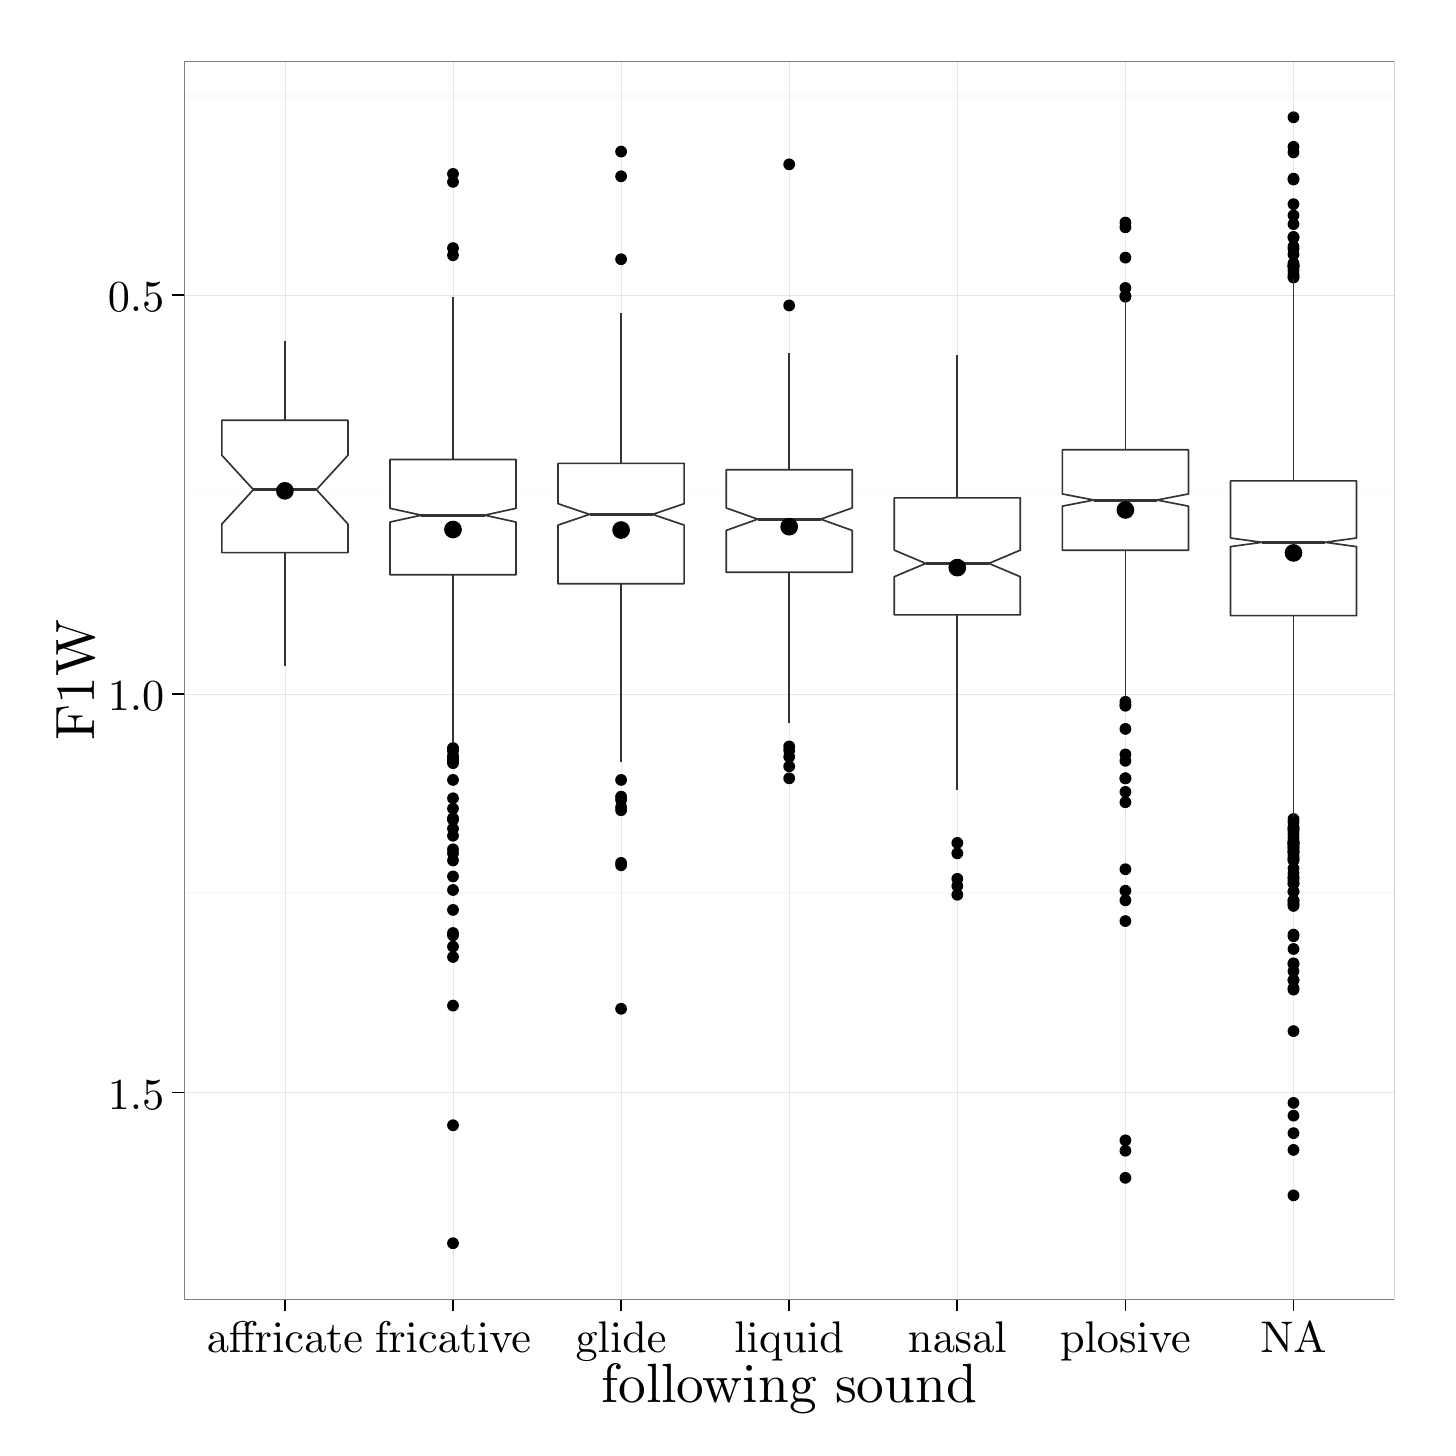
\begin{tikzpicture}[x=1pt,y=1pt]
\definecolor{fillColor}{RGB}{255,255,255}
\path[use as bounding box,fill=fillColor,fill opacity=0.00] (0,0) rectangle (505.89,505.89);
\begin{scope}
\path[clip] (  0.00,  0.00) rectangle (505.89,505.89);
\definecolor{drawColor}{RGB}{255,255,255}
\definecolor{fillColor}{RGB}{255,255,255}

\path[draw=drawColor,line width= 0.6pt,line join=round,line cap=round,fill=fillColor] (  0.00, -0.00) rectangle (505.89,505.89);
\end{scope}
\begin{scope}
\path[clip] ( 56.50, 46.31) rectangle (493.85,493.84);
\definecolor{fillColor}{RGB}{255,255,255}

\path[fill=fillColor] ( 56.50, 46.31) rectangle (493.85,493.84);
\definecolor{drawColor}{gray}{0.98}

\path[draw=drawColor,line width= 0.6pt,line join=round] ( 56.50,481.28) --
	(493.85,481.28);

\path[draw=drawColor,line width= 0.6pt,line join=round] ( 56.50,337.21) --
	(493.85,337.21);

\path[draw=drawColor,line width= 0.6pt,line join=round] ( 56.50,193.14) --
	(493.85,193.14);
\definecolor{drawColor}{gray}{0.90}

\path[draw=drawColor,line width= 0.2pt,line join=round] ( 56.50,409.25) --
	(493.85,409.25);

\path[draw=drawColor,line width= 0.2pt,line join=round] ( 56.50,265.18) --
	(493.85,265.18);

\path[draw=drawColor,line width= 0.2pt,line join=round] ( 56.50,121.11) --
	(493.85,121.11);

\path[draw=drawColor,line width= 0.2pt,line join=round] ( 92.95, 46.31) --
	( 92.95,493.84);

\path[draw=drawColor,line width= 0.2pt,line join=round] (153.69, 46.31) --
	(153.69,493.84);

\path[draw=drawColor,line width= 0.2pt,line join=round] (214.43, 46.31) --
	(214.43,493.84);

\path[draw=drawColor,line width= 0.2pt,line join=round] (275.17, 46.31) --
	(275.17,493.84);

\path[draw=drawColor,line width= 0.2pt,line join=round] (335.92, 46.31) --
	(335.92,493.84);

\path[draw=drawColor,line width= 0.2pt,line join=round] (396.66, 46.31) --
	(396.66,493.84);

\path[draw=drawColor,line width= 0.2pt,line join=round] (457.40, 46.31) --
	(457.40,493.84);
\definecolor{drawColor}{gray}{0.20}

\path[draw=drawColor,line width= 0.6pt,line join=round] ( 92.95,364.01) -- ( 92.95,392.54);

\path[draw=drawColor,line width= 0.6pt,line join=round] ( 92.95,316.18) -- ( 92.95,275.26);

\path[draw=drawColor,line width= 0.6pt,line join=round,line cap=round,fill=fillColor] ( 70.17,364.01) --
	( 70.17,351.37) --
	( 81.56,338.94) --
	( 70.17,326.52) --
	( 70.17,316.18) --
	(115.73,316.18) --
	(115.73,326.52) --
	(104.34,338.94) --
	(115.73,351.37) --
	(115.73,364.01) --
	( 70.17,364.01) --
	cycle;

\path[draw=drawColor,line width= 1.1pt,line join=round] ( 81.56,338.94) -- (104.34,338.94);
\definecolor{fillColor}{RGB}{0,0,0}

\path[fill=fillColor] (153.69,227.43) circle (  2.13);

\path[fill=fillColor] (153.69,240.69) circle (  2.13);

\path[fill=fillColor] (153.69,152.52) circle (  2.13);

\path[fill=fillColor] (153.69,213.89) circle (  2.13);

\path[fill=fillColor] (153.69,450.16) circle (  2.13);

\path[fill=fillColor] (153.69,245.58) circle (  2.13);

\path[fill=fillColor] (153.69,241.84) circle (  2.13);

\path[fill=fillColor] (153.69,220.23) circle (  2.13);

\path[fill=fillColor] (153.69,241.55) circle (  2.13);

\path[fill=fillColor] (153.69,244.43) circle (  2.13);

\path[fill=fillColor] (153.69,208.99) circle (  2.13);

\path[fill=fillColor] (153.69,216.48) circle (  2.13);

\path[fill=fillColor] (153.69,223.69) circle (  2.13);

\path[fill=fillColor] (153.69,240.11) circle (  2.13);

\path[fill=fillColor] (153.69,242.70) circle (  2.13);

\path[fill=fillColor] (153.69,207.55) circle (  2.13);

\path[fill=fillColor] (153.69, 66.65) circle (  2.13);

\path[fill=fillColor] (153.69,177.87) circle (  2.13);

\path[fill=fillColor] (153.69,109.29) circle (  2.13);

\path[fill=fillColor] (153.69,245.30) circle (  2.13);

\path[fill=fillColor] (153.69,219.65) circle (  2.13);

\path[fill=fillColor] (153.69,199.19) circle (  2.13);

\path[fill=fillColor] (153.69,170.09) circle (  2.13);

\path[fill=fillColor] (153.69,241.84) circle (  2.13);

\path[fill=fillColor] (153.69,423.65) circle (  2.13);

\path[fill=fillColor] (153.69,426.25) circle (  2.13);

\path[fill=fillColor] (153.69,453.04) circle (  2.13);

\path[fill=fillColor] (153.69,178.74) circle (  2.13);

\path[fill=fillColor] (153.69,194.30) circle (  2.13);

\path[fill=fillColor] (153.69,187.09) circle (  2.13);

\path[fill=fillColor] (153.69,173.84) circle (  2.13);

\path[fill=fillColor] (153.69,204.96) circle (  2.13);

\path[fill=fillColor] (153.69,234.06) circle (  2.13);

\path[draw=drawColor,line width= 0.6pt,line join=round] (153.69,349.82) -- (153.69,408.67);

\path[draw=drawColor,line width= 0.6pt,line join=round] (153.69,308.18) -- (153.69,247.89);
\definecolor{fillColor}{RGB}{255,255,255}

\path[draw=drawColor,line width= 0.6pt,line join=round,line cap=round,fill=fillColor] (130.91,349.82) --
	(130.91,332.20) --
	(142.30,329.72) --
	(130.91,327.24) --
	(130.91,308.18) --
	(176.47,308.18) --
	(176.47,327.24) --
	(165.08,329.72) --
	(176.47,332.20) --
	(176.47,349.82) --
	(130.91,349.82) --
	cycle;

\path[draw=drawColor,line width= 1.1pt,line join=round] (142.30,329.72) -- (165.08,329.72);
\definecolor{fillColor}{RGB}{0,0,0}

\path[fill=fillColor] (214.43,204.09) circle (  2.13);

\path[fill=fillColor] (214.43,228.01) circle (  2.13);

\path[fill=fillColor] (214.43,422.21) circle (  2.13);

\path[fill=fillColor] (214.43,203.23) circle (  2.13);

\path[fill=fillColor] (214.43,452.18) circle (  2.13);

\path[fill=fillColor] (214.43,223.11) circle (  2.13);

\path[fill=fillColor] (214.43,224.26) circle (  2.13);

\path[fill=fillColor] (214.43,151.36) circle (  2.13);

\path[fill=fillColor] (214.43,461.11) circle (  2.13);

\path[fill=fillColor] (214.43,226.86) circle (  2.13);

\path[fill=fillColor] (214.43,234.06) circle (  2.13);

\path[draw=drawColor,line width= 0.6pt,line join=round] (214.43,348.45) -- (214.43,402.62);

\path[draw=drawColor,line width= 0.6pt,line join=round] (214.43,304.94) -- (214.43,240.69);
\definecolor{fillColor}{RGB}{255,255,255}

\path[draw=drawColor,line width= 0.6pt,line join=round,line cap=round,fill=fillColor] (191.65,348.45) --
	(191.65,333.87) --
	(203.04,330.01) --
	(191.65,326.15) --
	(191.65,304.94) --
	(237.21,304.94) --
	(237.21,326.15) --
	(225.82,330.01) --
	(237.21,333.87) --
	(237.21,348.45) --
	(191.65,348.45) --
	cycle;

\path[draw=drawColor,line width= 1.1pt,line join=round] (203.04,330.01) -- (225.82,330.01);
\definecolor{fillColor}{RGB}{0,0,0}

\path[fill=fillColor] (275.17,246.16) circle (  2.13);

\path[fill=fillColor] (275.17,456.50) circle (  2.13);

\path[fill=fillColor] (275.17,234.64) circle (  2.13);

\path[fill=fillColor] (275.17,405.50) circle (  2.13);

\path[fill=fillColor] (275.17,244.72) circle (  2.13);

\path[fill=fillColor] (275.17,242.41) circle (  2.13);

\path[fill=fillColor] (275.17,238.96) circle (  2.13);

\path[draw=drawColor,line width= 0.6pt,line join=round] (275.17,346.14) -- (275.17,388.50);

\path[draw=drawColor,line width= 0.6pt,line join=round] (275.17,309.12) -- (275.17,254.52);
\definecolor{fillColor}{RGB}{255,255,255}

\path[draw=drawColor,line width= 0.6pt,line join=round,line cap=round,fill=fillColor] (252.40,346.14) --
	(252.40,332.35) --
	(263.79,328.28) --
	(252.40,324.21) --
	(252.40,309.12) --
	(297.95,309.12) --
	(297.95,324.21) --
	(286.56,328.28) --
	(297.95,332.35) --
	(297.95,346.14) --
	(252.40,346.14) --
	cycle;

\path[draw=drawColor,line width= 1.1pt,line join=round] (263.79,328.28) -- (286.56,328.28);
\definecolor{fillColor}{RGB}{0,0,0}

\path[fill=fillColor] (335.92,207.55) circle (  2.13);

\path[fill=fillColor] (335.92,192.57) circle (  2.13);

\path[fill=fillColor] (335.92,195.74) circle (  2.13);

\path[fill=fillColor] (335.92,211.30) circle (  2.13);

\path[fill=fillColor] (335.92,198.33) circle (  2.13);

\path[draw=drawColor,line width= 0.6pt,line join=round] (335.92,335.99) -- (335.92,387.64);

\path[draw=drawColor,line width= 0.6pt,line join=round] (335.92,293.70) -- (335.92,230.31);
\definecolor{fillColor}{RGB}{255,255,255}

\path[draw=drawColor,line width= 0.6pt,line join=round,line cap=round,fill=fillColor] (313.14,335.99) --
	(313.14,317.09) --
	(324.53,312.29) --
	(313.14,307.49) --
	(313.14,293.70) --
	(358.69,293.70) --
	(358.69,307.49) --
	(347.31,312.29) --
	(358.69,317.09) --
	(358.69,335.99) --
	(313.14,335.99) --
	cycle;

\path[draw=drawColor,line width= 1.1pt,line join=round] (324.53,312.29) -- (347.31,312.29);
\definecolor{fillColor}{RGB}{0,0,0}

\path[fill=fillColor] (396.66,408.67) circle (  2.13);

\path[fill=fillColor] (396.66,243.28) circle (  2.13);

\path[fill=fillColor] (396.66,260.86) circle (  2.13);

\path[fill=fillColor] (396.66,435.47) circle (  2.13);

\path[fill=fillColor] (396.66,190.55) circle (  2.13);

\path[fill=fillColor] (396.66,261.14) circle (  2.13);

\path[fill=fillColor] (396.66,201.79) circle (  2.13);

\path[fill=fillColor] (396.66,234.64) circle (  2.13);

\path[fill=fillColor] (396.66,408.96) circle (  2.13);

\path[fill=fillColor] (396.66,411.84) circle (  2.13);

\path[fill=fillColor] (396.66, 90.28) circle (  2.13);

\path[fill=fillColor] (396.66,194.01) circle (  2.13);

\path[fill=fillColor] (396.66,100.07) circle (  2.13);

\path[fill=fillColor] (396.66,252.50) circle (  2.13);

\path[fill=fillColor] (396.66,103.82) circle (  2.13);

\path[fill=fillColor] (396.66,422.79) circle (  2.13);

\path[fill=fillColor] (396.66,229.74) circle (  2.13);

\path[fill=fillColor] (396.66,234.64) circle (  2.13);

\path[fill=fillColor] (396.66,240.97) circle (  2.13);

\path[fill=fillColor] (396.66,262.30) circle (  2.13);

\path[fill=fillColor] (396.66,433.74) circle (  2.13);

\path[fill=fillColor] (396.66,183.06) circle (  2.13);

\path[fill=fillColor] (396.66,225.99) circle (  2.13);

\path[draw=drawColor,line width= 0.6pt,line join=round] (396.66,353.35) -- (396.66,407.52);

\path[draw=drawColor,line width= 0.6pt,line join=round] (396.66,317.04) -- (396.66,264.03);
\definecolor{fillColor}{RGB}{255,255,255}

\path[draw=drawColor,line width= 0.6pt,line join=round,line cap=round,fill=fillColor] (373.88,353.35) --
	(373.88,337.40) --
	(385.27,335.20) --
	(373.88,332.99) --
	(373.88,317.04) --
	(419.44,317.04) --
	(419.44,332.99) --
	(408.05,335.20) --
	(419.44,337.40) --
	(419.44,353.35) --
	(373.88,353.35) --
	cycle;

\path[draw=drawColor,line width= 1.1pt,line join=round] (385.27,335.20) -- (408.05,335.20);
\definecolor{fillColor}{RGB}{0,0,0}

\path[fill=fillColor] (457.40,209.57) circle (  2.13);

\path[fill=fillColor] (457.40,200.35) circle (  2.13);

\path[fill=fillColor] (457.40,212.16) circle (  2.13);

\path[fill=fillColor] (457.40,473.50) circle (  2.13);

\path[fill=fillColor] (457.40,193.72) circle (  2.13);

\path[fill=fillColor] (457.40,415.87) circle (  2.13);

\path[fill=fillColor] (457.40,205.82) circle (  2.13);

\path[fill=fillColor] (457.40,189.69) circle (  2.13);

\path[fill=fillColor] (457.40,216.19) circle (  2.13);

\path[fill=fillColor] (457.40,218.79) circle (  2.13);

\path[fill=fillColor] (457.40,211.30) circle (  2.13);

\path[fill=fillColor] (457.40,442.10) circle (  2.13);

\path[fill=fillColor] (457.40,429.99) circle (  2.13);

\path[fill=fillColor] (457.40,434.89) circle (  2.13);

\path[fill=fillColor] (457.40,158.28) circle (  2.13);

\path[fill=fillColor] (457.40,215.62) circle (  2.13);

\path[fill=fillColor] (457.40,198.62) circle (  2.13);

\path[fill=fillColor] (457.40,217.06) circle (  2.13);

\path[fill=fillColor] (457.40,216.77) circle (  2.13);

\path[fill=fillColor] (457.40,206.69) circle (  2.13);

\path[fill=fillColor] (457.40,219.94) circle (  2.13);

\path[fill=fillColor] (457.40,197.75) circle (  2.13);

\path[fill=fillColor] (457.40,189.11) circle (  2.13);

\path[fill=fillColor] (457.40,143.30) circle (  2.13);

\path[fill=fillColor] (457.40,214.47) circle (  2.13);

\path[fill=fillColor] (457.40,190.55) circle (  2.13);

\path[fill=fillColor] (457.40, 83.94) circle (  2.13);

\path[fill=fillColor] (457.40,205.24) circle (  2.13);

\path[fill=fillColor] (457.40,100.36) circle (  2.13);

\path[fill=fillColor] (457.40,112.75) circle (  2.13);

\path[fill=fillColor] (457.40,196.60) circle (  2.13);

\path[fill=fillColor] (457.40,117.36) circle (  2.13);

\path[fill=fillColor] (457.40,106.41) circle (  2.13);

\path[fill=fillColor] (457.40,211.30) circle (  2.13);

\path[fill=fillColor] (457.40,188.53) circle (  2.13);

\path[fill=fillColor] (457.40,210.43) circle (  2.13);

\path[fill=fillColor] (457.40,190.55) circle (  2.13);

\path[fill=fillColor] (457.40,198.91) circle (  2.13);

\path[fill=fillColor] (457.40,211.01) circle (  2.13);

\path[fill=fillColor] (457.40,196.60) circle (  2.13);

\path[fill=fillColor] (457.40,418.18) circle (  2.13);

\path[fill=fillColor] (457.40,419.33) circle (  2.13);

\path[fill=fillColor] (457.40,416.74) circle (  2.13);

\path[fill=fillColor] (457.40,419.62) circle (  2.13);

\path[fill=fillColor] (457.40,167.50) circle (  2.13);

\path[fill=fillColor] (457.40,161.74) circle (  2.13);

\path[fill=fillColor] (457.40,425.96) circle (  2.13);

\path[fill=fillColor] (457.40,419.91) circle (  2.13);

\path[fill=fillColor] (457.40,164.91) circle (  2.13);

\path[fill=fillColor] (457.40,178.16) circle (  2.13);

\path[fill=fillColor] (457.40,420.77) circle (  2.13);

\path[fill=fillColor] (457.40,202.08) circle (  2.13);

\path[fill=fillColor] (457.40,426.82) circle (  2.13);

\path[fill=fillColor] (457.40,208.13) circle (  2.13);

\path[fill=fillColor] (457.40,158.85) circle (  2.13);

\path[fill=fillColor] (457.40,415.59) circle (  2.13);

\path[fill=fillColor] (457.40,177.58) circle (  2.13);

\path[fill=fillColor] (457.40,161.74) circle (  2.13);

\path[fill=fillColor] (457.40,167.79) circle (  2.13);

\path[fill=fillColor] (457.40,438.06) circle (  2.13);

\path[fill=fillColor] (457.40,462.84) circle (  2.13);

\path[fill=fillColor] (457.40,419.91) circle (  2.13);

\path[fill=fillColor] (457.40,451.32) circle (  2.13);

\path[fill=fillColor] (457.40,460.82) circle (  2.13);

\path[fill=fillColor] (457.40,430.28) circle (  2.13);

\path[fill=fillColor] (457.40,423.94) circle (  2.13);

\path[fill=fillColor] (457.40,209.86) circle (  2.13);

\path[fill=fillColor] (457.40,208.99) circle (  2.13);

\path[fill=fillColor] (457.40,211.30) circle (  2.13);

\path[fill=fillColor] (457.40,208.13) circle (  2.13);

\path[fill=fillColor] (457.40,172.97) circle (  2.13);

\path[fill=fillColor] (457.40,207.84) circle (  2.13);

\path[fill=fillColor] (457.40,451.03) circle (  2.13);

\path[fill=fillColor] (457.40,213.31) circle (  2.13);

\path[fill=fillColor] (457.40,204.96) circle (  2.13);

\path[fill=fillColor] (457.40,193.72) circle (  2.13);

\path[draw=drawColor,line width= 0.6pt,line join=round] (457.40,342.11) -- (457.40,415.01);

\path[draw=drawColor,line width= 0.6pt,line join=round] (457.40,293.42) -- (457.40,220.52);
\definecolor{fillColor}{RGB}{255,255,255}

\path[draw=drawColor,line width= 0.6pt,line join=round,line cap=round,fill=fillColor] (434.62,342.11) --
	(434.62,321.48) --
	(446.01,319.92) --
	(434.62,318.36) --
	(434.62,293.42) --
	(480.18,293.42) --
	(480.18,318.36) --
	(468.79,319.92) --
	(480.18,321.48) --
	(480.18,342.11) --
	(434.62,342.11) --
	cycle;

\path[draw=drawColor,line width= 1.1pt,line join=round] (446.01,319.92) -- (468.79,319.92);
\definecolor{fillColor}{RGB}{0,0,0}

\path[fill=fillColor] ( 92.95,338.52) circle (  3.20);

\path[fill=fillColor] (153.69,324.54) circle (  3.20);

\path[fill=fillColor] (214.43,324.36) circle (  3.20);

\path[fill=fillColor] (275.17,325.56) circle (  3.20);

\path[fill=fillColor] (335.92,310.78) circle (  3.20);

\path[fill=fillColor] (396.66,331.61) circle (  3.20);

\path[fill=fillColor] (457.40,316.08) circle (  3.20);
\definecolor{drawColor}{gray}{0.50}

\path[draw=drawColor,line width= 0.6pt,line join=round,line cap=round] ( 56.50, 46.31) rectangle (493.85,493.84);
\end{scope}
\begin{scope}
\path[clip] (  0.00,  0.00) rectangle (505.89,505.89);
\definecolor{drawColor}{RGB}{0,0,0}

\node[text=drawColor,anchor=base east,inner sep=0pt, outer sep=0pt, scale=  1.60] at ( 49.39,403.21) {0.5};

\node[text=drawColor,anchor=base east,inner sep=0pt, outer sep=0pt, scale=  1.60] at ( 49.39,259.14) {1.0};

\node[text=drawColor,anchor=base east,inner sep=0pt, outer sep=0pt, scale=  1.60] at ( 49.39,115.08) {1.5};
\end{scope}
\begin{scope}
\path[clip] (  0.00,  0.00) rectangle (505.89,505.89);
\definecolor{drawColor}{RGB}{0,0,0}

\path[draw=drawColor,line width= 0.6pt,line join=round] ( 52.24,409.25) --
	( 56.50,409.25);

\path[draw=drawColor,line width= 0.6pt,line join=round] ( 52.24,265.18) --
	( 56.50,265.18);

\path[draw=drawColor,line width= 0.6pt,line join=round] ( 52.24,121.11) --
	( 56.50,121.11);
\end{scope}
\begin{scope}
\path[clip] (  0.00,  0.00) rectangle (505.89,505.89);
\definecolor{drawColor}{RGB}{0,0,0}

\path[draw=drawColor,line width= 0.6pt,line join=round] ( 92.95, 42.04) --
	( 92.95, 46.31);

\path[draw=drawColor,line width= 0.6pt,line join=round] (153.69, 42.04) --
	(153.69, 46.31);

\path[draw=drawColor,line width= 0.6pt,line join=round] (214.43, 42.04) --
	(214.43, 46.31);

\path[draw=drawColor,line width= 0.6pt,line join=round] (275.17, 42.04) --
	(275.17, 46.31);

\path[draw=drawColor,line width= 0.6pt,line join=round] (335.92, 42.04) --
	(335.92, 46.31);

\path[draw=drawColor,line width= 0.6pt,line join=round] (396.66, 42.04) --
	(396.66, 46.31);

\path[draw=drawColor,line width= 0.6pt,line join=round] (457.40, 42.04) --
	(457.40, 46.31);
\end{scope}
\begin{scope}
\path[clip] (  0.00,  0.00) rectangle (505.89,505.89);
\definecolor{drawColor}{RGB}{0,0,0}

\node[text=drawColor,anchor=base,inner sep=0pt, outer sep=0pt, scale=  1.60] at ( 92.95, 27.13) {affricate};

\node[text=drawColor,anchor=base,inner sep=0pt, outer sep=0pt, scale=  1.60] at (153.69, 27.13) {fricative};

\node[text=drawColor,anchor=base,inner sep=0pt, outer sep=0pt, scale=  1.60] at (214.43, 27.13) {glide};

\node[text=drawColor,anchor=base,inner sep=0pt, outer sep=0pt, scale=  1.60] at (275.17, 27.13) {liquid};

\node[text=drawColor,anchor=base,inner sep=0pt, outer sep=0pt, scale=  1.60] at (335.92, 27.13) {nasal};

\node[text=drawColor,anchor=base,inner sep=0pt, outer sep=0pt, scale=  1.60] at (396.66, 27.13) {plosive};

\node[text=drawColor,anchor=base,inner sep=0pt, outer sep=0pt, scale=  1.60] at (457.40, 27.13) {NA};
\end{scope}
\begin{scope}
\path[clip] (  0.00,  0.00) rectangle (505.89,505.89);
\definecolor{drawColor}{RGB}{0,0,0}

\node[text=drawColor,anchor=base,inner sep=0pt, outer sep=0pt, scale=  2.00] at (275.17,  9.03) {following sound};
\end{scope}
\begin{scope}
\path[clip] (  0.00,  0.00) rectangle (505.89,505.89);
\definecolor{drawColor}{RGB}{0,0,0}

\node[text=drawColor,rotate= 90.00,anchor=base,inner sep=0pt, outer sep=0pt, scale=  2.00] at ( 24.12,270.08) {F1W};
\end{scope}
\end{tikzpicture}
} 
		\caption{happ\textsc{y} (F1) by following sound}
		\label{fig.box.f1w.happy.follsound}
	\end{figure}

Figure \ref{fig.box.f1w.happy.follsound} shows normalise\is{normalisation}d F1 values on the y-axis, and the manner of the consonant that follows the test vowel on the x-axis.
Just as in the mixed-effects model, only two levels of this factor really stand out: when happ\textsc{y} is followed by an affricate F1 values are slightly lower, i.e. the vowel is a bit higher, whereas when happ\textsc{y} precedes a nasal, F1 is significantly higher, so the vowel is somewhat lower.
All the other contexts have similar means (black dots) and medians (black horizontal bars around the middle of the boxes), and do not differ significantly from each other.
It is unclear why happ\textsc{y} should be higher when the following word (happ\textsc{y} is, of course, always word-final\is{phonological context}) starts with an affricate, but it should be noted that the number of observations in this sub-category is rather small anyway (n = 37), so these figures might not be very representative.
For nasals, on the other hand, this is less of an argument, as there are much more data in this sample (n = 194), but here the shift can potentially be explained on phonetic grounds.
As an effect of regressive assimilation, it is likely that happ\textsc{y} exhibits some degree of nasalisation when it occurs before a nasal, and nasalisation is know to shift F1 upwards \parencite{housestevens1956}, which explains the difference visible in the graph.
Interestingly, F1 seems to be very similar in cases when happ\textsc{y} is not directly followed by anything because it is the last sound in a stretch of speech (this context is coded as ``NA'' in Figure \ref{fig.box.f1w.happy.follsound}), but it is a lot less straightforward why happ\textsc{y} should be lower before a pause.

	\begin{figure}[h!]
		\centering
		\definecolor{shadecolor}{rgb}{0.969, 0.969, 0.969}
		\resizebox{0.5\linewidth}{!}{% Created by tikzDevice version 0.8.1 on 2016-02-09 02:12:04
% !TEX encoding = UTF-8 Unicode
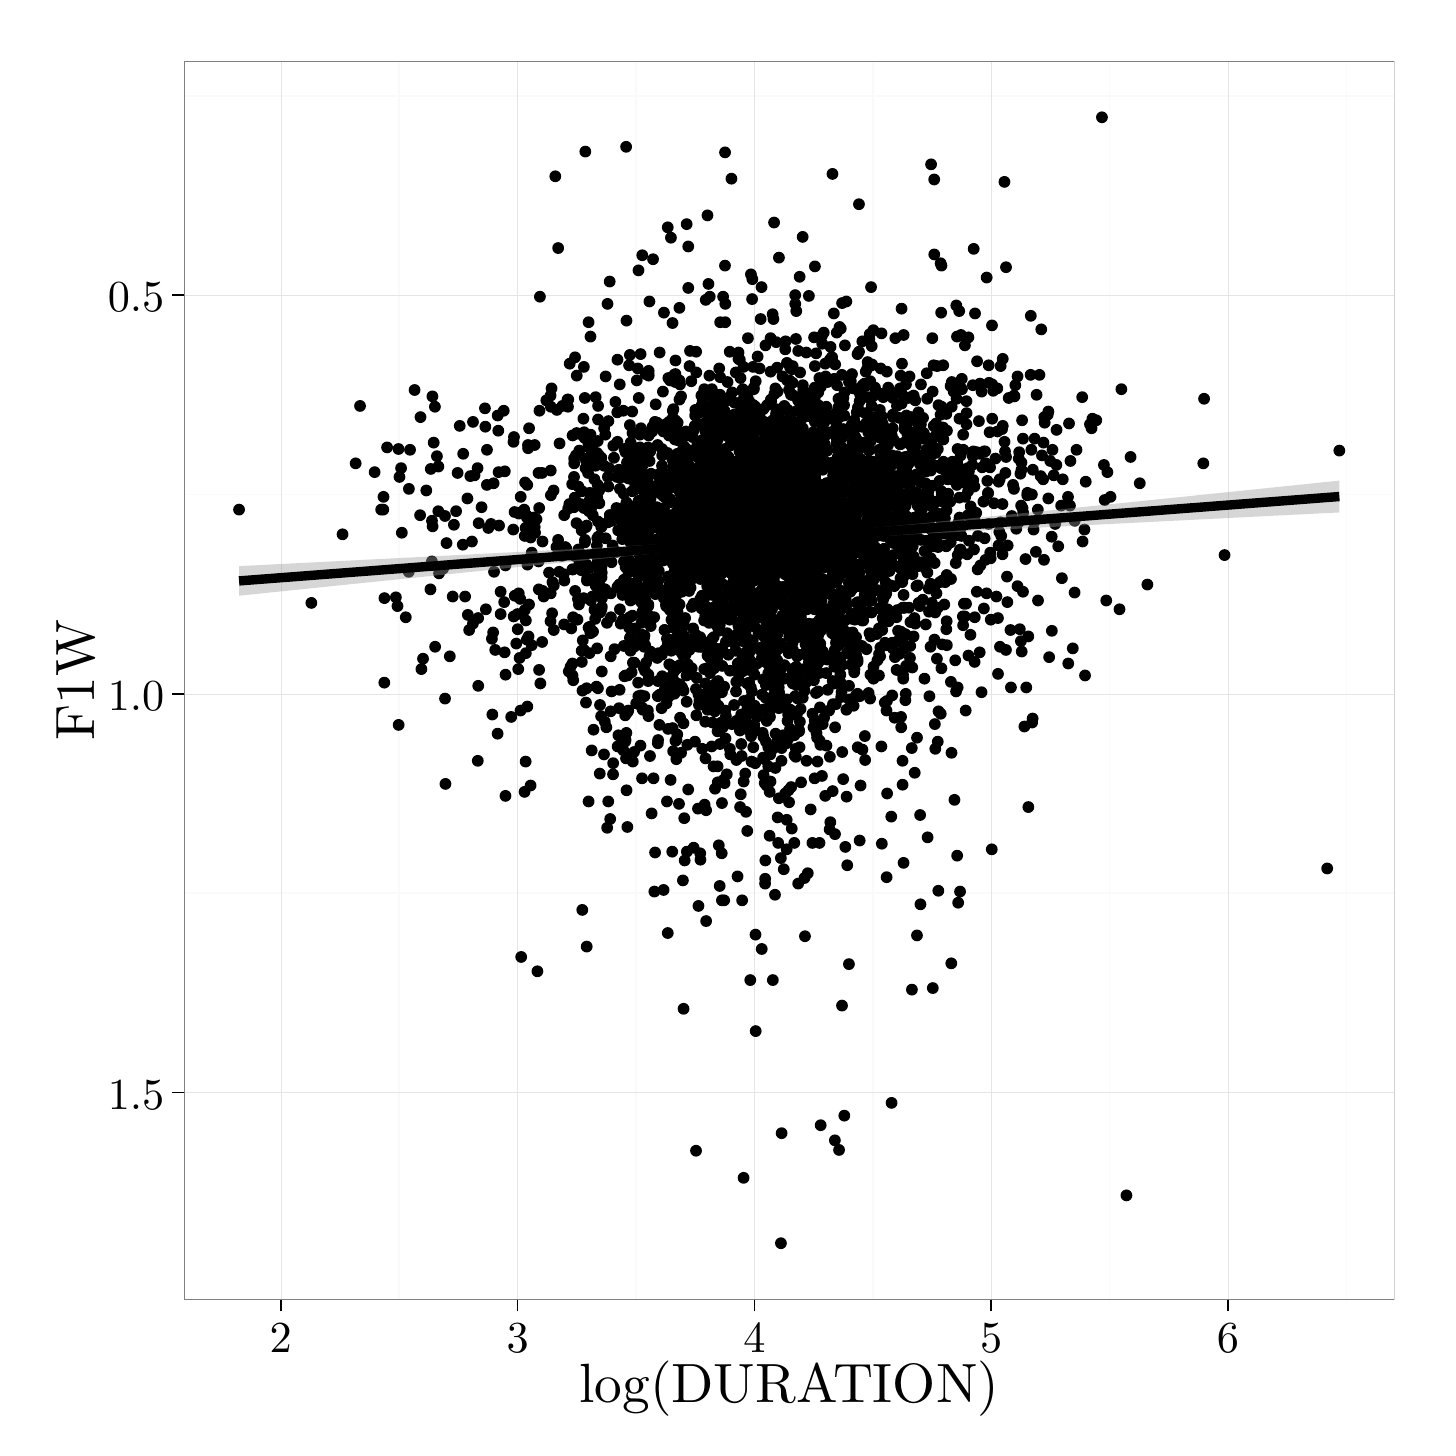
\begin{tikzpicture}[x=1pt,y=1pt]
\definecolor{fillColor}{RGB}{255,255,255}
\path[use as bounding box,fill=fillColor,fill opacity=0.00] (0,0) rectangle (505.89,505.89);
\begin{scope}
\path[clip] (  0.00,  0.00) rectangle (505.89,505.89);
\definecolor{drawColor}{RGB}{255,255,255}
\definecolor{fillColor}{RGB}{255,255,255}

\path[draw=drawColor,line width= 0.6pt,line join=round,line cap=round,fill=fillColor] (  0.00, -0.00) rectangle (505.89,505.89);
\end{scope}
\begin{scope}
\path[clip] ( 56.50, 46.31) rectangle (493.85,493.84);
\definecolor{fillColor}{RGB}{255,255,255}

\path[fill=fillColor] ( 56.50, 46.31) rectangle (493.85,493.84);
\definecolor{drawColor}{gray}{0.98}

\path[draw=drawColor,line width= 0.6pt,line join=round] ( 56.50,481.28) --
	(493.85,481.28);

\path[draw=drawColor,line width= 0.6pt,line join=round] ( 56.50,337.21) --
	(493.85,337.21);

\path[draw=drawColor,line width= 0.6pt,line join=round] ( 56.50,193.14) --
	(493.85,193.14);

\path[draw=drawColor,line width= 0.6pt,line join=round] (134.25, 46.31) --
	(134.25,493.84);

\path[draw=drawColor,line width= 0.6pt,line join=round] (219.82, 46.31) --
	(219.82,493.84);

\path[draw=drawColor,line width= 0.6pt,line join=round] (305.39, 46.31) --
	(305.39,493.84);

\path[draw=drawColor,line width= 0.6pt,line join=round] (390.96, 46.31) --
	(390.96,493.84);

\path[draw=drawColor,line width= 0.6pt,line join=round] (476.53, 46.31) --
	(476.53,493.84);
\definecolor{drawColor}{gray}{0.90}

\path[draw=drawColor,line width= 0.2pt,line join=round] ( 56.50,409.25) --
	(493.85,409.25);

\path[draw=drawColor,line width= 0.2pt,line join=round] ( 56.50,265.18) --
	(493.85,265.18);

\path[draw=drawColor,line width= 0.2pt,line join=round] ( 56.50,121.11) --
	(493.85,121.11);

\path[draw=drawColor,line width= 0.2pt,line join=round] ( 91.47, 46.31) --
	( 91.47,493.84);

\path[draw=drawColor,line width= 0.2pt,line join=round] (177.04, 46.31) --
	(177.04,493.84);

\path[draw=drawColor,line width= 0.2pt,line join=round] (262.61, 46.31) --
	(262.61,493.84);

\path[draw=drawColor,line width= 0.2pt,line join=round] (348.17, 46.31) --
	(348.17,493.84);

\path[draw=drawColor,line width= 0.2pt,line join=round] (433.74, 46.31) --
	(433.74,493.84);
\definecolor{fillColor}{RGB}{0,0,0}

\path[fill=fillColor] (265.89,355.37) circle (  2.13);

\path[fill=fillColor] (242.20,313.30) circle (  2.13);

\path[fill=fillColor] (310.24,301.48) circle (  2.13);

\path[fill=fillColor] (248.44,312.72) circle (  2.13);

\path[fill=fillColor] (258.41,279.01) circle (  2.13);

\path[fill=fillColor] (258.61,336.64) circle (  2.13);

\path[fill=fillColor] (293.12,282.75) circle (  2.13);

\path[fill=fillColor] (274.60,318.20) circle (  2.13);

\path[fill=fillColor] (188.93,291.40) circle (  2.13);

\path[fill=fillColor] (215.71,329.43) circle (  2.13);

\path[fill=fillColor] (278.38,341.25) circle (  2.13);

\path[fill=fillColor] (266.80,291.40) circle (  2.13);

\path[fill=fillColor] (246.47,278.14) circle (  2.13);

\path[fill=fillColor] (269.81,269.21) circle (  2.13);

\path[fill=fillColor] (257.44,323.38) circle (  2.13);

\path[fill=fillColor] (180.02,291.69) circle (  2.13);

\path[fill=fillColor] (219.88,261.72) circle (  2.13);

\path[fill=fillColor] (198.33,326.84) circle (  2.13);

\path[fill=fillColor] (252.78,324.53) circle (  2.13);

\path[fill=fillColor] (330.25,368.91) circle (  2.13);

\path[fill=fillColor] (249.12,291.40) circle (  2.13);

\path[fill=fillColor] (288.55,334.33) circle (  2.13);

\path[fill=fillColor] (240.66,209.57) circle (  2.13);

\path[fill=fillColor] (230.15,330.01) circle (  2.13);

\path[fill=fillColor] (241.44,286.50) circle (  2.13);

\path[fill=fillColor] (364.32,316.47) circle (  2.13);

\path[fill=fillColor] (247.52,274.97) circle (  2.13);

\path[fill=fillColor] (202.68,226.28) circle (  2.13);

\path[fill=fillColor] (264.19,314.16) circle (  2.13);

\path[fill=fillColor] (249.45,265.47) circle (  2.13);

\path[fill=fillColor] (279.98,313.01) circle (  2.13);

\path[fill=fillColor] (267.10,323.38) circle (  2.13);

\path[fill=fillColor] (269.18,402.33) circle (  2.13);

\path[fill=fillColor] (218.70,324.25) circle (  2.13);

\path[fill=fillColor] (243.02,207.55) circle (  2.13);

\path[fill=fillColor] (299.93,245.87) circle (  2.13);

\path[fill=fillColor] (262.53,253.94) circle (  2.13);

\path[fill=fillColor] (240.12,284.48) circle (  2.13);

\path[fill=fillColor] (281.89,200.35) circle (  2.13);

\path[fill=fillColor] (322.36,296.87) circle (  2.13);

\path[fill=fillColor] (277.46,269.50) circle (  2.13);

\path[fill=fillColor] (306.61,334.04) circle (  2.13);

\path[fill=fillColor] (257.19,352.77) circle (  2.13);

\path[fill=fillColor] (279.44,302.35) circle (  2.13);

\path[fill=fillColor] (274.79,342.11) circle (  2.13);

\path[fill=fillColor] (252.55,296.59) circle (  2.13);

\path[fill=fillColor] (242.02,323.67) circle (  2.13);

\path[fill=fillColor] (277.58,245.30) circle (  2.13);

\path[fill=fillColor] (227.33,338.37) circle (  2.13);

\path[fill=fillColor] (267.12,286.79) circle (  2.13);

\path[fill=fillColor] (251.33,304.65) circle (  2.13);

\path[fill=fillColor] (250.16,247.03) circle (  2.13);

\path[fill=fillColor] (252.05,259.13) circle (  2.13);

\path[fill=fillColor] (263.58,276.13) circle (  2.13);

\path[fill=fillColor] (287.43,325.69) circle (  2.13);

\path[fill=fillColor] (224.34,270.65) circle (  2.13);

\path[fill=fillColor] (178.09,259.13) circle (  2.13);

\path[fill=fillColor] (260.54,298.03) circle (  2.13);

\path[fill=fillColor] (212.77,332.31) circle (  2.13);

\path[fill=fillColor] (289.07,302.64) circle (  2.13);

\path[fill=fillColor] (247.87,303.21) circle (  2.13);

\path[fill=fillColor] (265.07,354.50) circle (  2.13);

\path[fill=fillColor] (285.05,314.16) circle (  2.13);

\path[fill=fillColor] (242.57,333.75) circle (  2.13);

\path[fill=fillColor] (247.33,327.42) circle (  2.13);

\path[fill=fillColor] (244.77,353.64) circle (  2.13);

\path[fill=fillColor] (292.18,337.21) circle (  2.13);

\path[fill=fillColor] (298.63,319.06) circle (  2.13);

\path[fill=fillColor] (275.50,377.84) circle (  2.13);

\path[fill=fillColor] (269.81,284.20) circle (  2.13);

\path[fill=fillColor] (253.95,361.70) circle (  2.13);

\path[fill=fillColor] (290.04,277.86) circle (  2.13);

\path[fill=fillColor] (258.16,340.96) circle (  2.13);

\path[fill=fillColor] (246.41,302.64) circle (  2.13);

\path[fill=fillColor] (243.56,369.48) circle (  2.13);

\path[fill=fillColor] (224.28,297.45) circle (  2.13);

\path[fill=fillColor] (249.09,327.70) circle (  2.13);

\path[fill=fillColor] (266.53,321.08) circle (  2.13);

\path[fill=fillColor] (250.30,291.40) circle (  2.13);

\path[fill=fillColor] (234.76,329.14) circle (  2.13);

\path[fill=fillColor] (280.64,354.79) circle (  2.13);

\path[fill=fillColor] (189.30,375.54) circle (  2.13);

\path[fill=fillColor] (266.36,314.45) circle (  2.13);

\path[fill=fillColor] (278.14,337.79) circle (  2.13);

\path[fill=fillColor] (266.31,326.26) circle (  2.13);

\path[fill=fillColor] (245.14,314.74) circle (  2.13);

\path[fill=fillColor] (180.52,340.67) circle (  2.13);

\path[fill=fillColor] (218.24,272.96) circle (  2.13);

\path[fill=fillColor] (216.59,330.87) circle (  2.13);

\path[fill=fillColor] (245.20,322.23) circle (  2.13);

\path[fill=fillColor] (245.29,264.03) circle (  2.13);

\path[fill=fillColor] (181.18,361.13) circle (  2.13);

\path[fill=fillColor] (229.93,332.31) circle (  2.13);

\path[fill=fillColor] (302.59,366.60) circle (  2.13);

\path[fill=fillColor] (257.88,332.31) circle (  2.13);

\path[fill=fillColor] (259.38,287.36) circle (  2.13);

\path[fill=fillColor] (243.07,306.67) circle (  2.13);

\path[fill=fillColor] (311.80,283.33) circle (  2.13);

\path[fill=fillColor] (237.95,339.81) circle (  2.13);

\path[fill=fillColor] (237.23,336.64) circle (  2.13);

\path[fill=fillColor] (210.98,312.72) circle (  2.13);

\path[fill=fillColor] (186.03,320.21) circle (  2.13);

\path[fill=fillColor] (218.79,332.89) circle (  2.13);

\path[fill=fillColor] (213.95,304.36) circle (  2.13);

\path[fill=fillColor] (233.87,309.84) circle (  2.13);

\path[fill=fillColor] (242.33,282.18) circle (  2.13);

\path[fill=fillColor] (245.47,274.40) circle (  2.13);

\path[fill=fillColor] (333.35,334.62) circle (  2.13);

\path[fill=fillColor] (244.37,299.47) circle (  2.13);

\path[fill=fillColor] (241.48,266.91) circle (  2.13);

\path[fill=fillColor] (238.09,271.81) circle (  2.13);

\path[fill=fillColor] (272.92,319.35) circle (  2.13);

\path[fill=fillColor] (316.21,346.14) circle (  2.13);

\path[fill=fillColor] (272.38,297.45) circle (  2.13);

\path[fill=fillColor] (297.22,327.13) circle (  2.13);

\path[fill=fillColor] (254.33,328.86) circle (  2.13);

\path[fill=fillColor] (257.21,255.96) circle (  2.13);

\path[fill=fillColor] (247.78,296.30) circle (  2.13);

\path[fill=fillColor] (297.06,330.87) circle (  2.13);

\path[fill=fillColor] (243.24,321.94) circle (  2.13);

\path[fill=fillColor] (269.41,276.13) circle (  2.13);

\path[fill=fillColor] (251.43,365.74) circle (  2.13);

\path[fill=fillColor] (230.55,362.57) circle (  2.13);

\path[fill=fillColor] (235.60,322.52) circle (  2.13);

\path[fill=fillColor] (210.39,329.72) circle (  2.13);

\path[fill=fillColor] (293.49,316.18) circle (  2.13);

\path[fill=fillColor] (263.85,339.81) circle (  2.13);

\path[fill=fillColor] (298.69,337.50) circle (  2.13);

\path[fill=fillColor] (327.92,294.57) circle (  2.13);

\path[fill=fillColor] (270.49,368.04) circle (  2.13);

\path[fill=fillColor] (292.37,328.86) circle (  2.13);

\path[fill=fillColor] (312.90,319.64) circle (  2.13);

\path[fill=fillColor] (248.71,302.92) circle (  2.13);

\path[fill=fillColor] (270.54,298.60) circle (  2.13);

\path[fill=fillColor] (260.87,305.81) circle (  2.13);

\path[fill=fillColor] (300.64,212.16) circle (  2.13);

\path[fill=fillColor] (275.94,291.11) circle (  2.13);

\path[fill=fillColor] (230.82,261.72) circle (  2.13);

\path[fill=fillColor] (261.84,312.14) circle (  2.13);

\path[fill=fillColor] (233.88,342.11) circle (  2.13);

\path[fill=fillColor] (283.92,367.18) circle (  2.13);

\path[fill=fillColor] (265.37,276.99) circle (  2.13);

\path[fill=fillColor] (237.00,266.33) circle (  2.13);

\path[fill=fillColor] (270.23,348.45) circle (  2.13);

\path[fill=fillColor] (263.25,323.96) circle (  2.13);

\path[fill=fillColor] (257.20,341.82) circle (  2.13);

\path[fill=fillColor] (242.01,310.99) circle (  2.13);

\path[fill=fillColor] (241.69,341.25) circle (  2.13);

\path[fill=fillColor] (263.48,318.20) circle (  2.13);

\path[fill=fillColor] (219.83,310.42) circle (  2.13);

\path[fill=fillColor] (277.48,337.50) circle (  2.13);

\path[fill=fillColor] (342.11,340.09) circle (  2.13);

\path[fill=fillColor] (333.92,377.84) circle (  2.13);

\path[fill=fillColor] (262.63,301.48) circle (  2.13);

\path[fill=fillColor] (245.11,328.86) circle (  2.13);

\path[fill=fillColor] (283.28,350.18) circle (  2.13);

\path[fill=fillColor] (284.67,306.38) circle (  2.13);

\path[fill=fillColor] (235.46,318.20) circle (  2.13);

\path[fill=fillColor] (256.97,313.30) circle (  2.13);

\path[fill=fillColor] (234.60,307.53) circle (  2.13);

\path[fill=fillColor] (150.96,232.62) circle (  2.13);

\path[fill=fillColor] (281.68,329.14) circle (  2.13);

\path[fill=fillColor] (258.35,358.53) circle (  2.13);

\path[fill=fillColor] (250.07,360.26) circle (  2.13);

\path[fill=fillColor] (303.96,349.31) circle (  2.13);

\path[fill=fillColor] (259.52,323.38) circle (  2.13);

\path[fill=fillColor] (184.80,273.82) circle (  2.13);

\path[fill=fillColor] (266.05,310.42) circle (  2.13);

\path[fill=fillColor] (248.58,349.89) circle (  2.13);

\path[fill=fillColor] (311.27,344.99) circle (  2.13);

\path[fill=fillColor] (273.75,389.65) circle (  2.13);

\path[fill=fillColor] (291.30,402.62) circle (  2.13);

\path[fill=fillColor] (259.26,311.57) circle (  2.13);

\path[fill=fillColor] (246.46,373.23) circle (  2.13);

\path[fill=fillColor] (218.52,347.87) circle (  2.13);

\path[fill=fillColor] (224.87,242.70) circle (  2.13);

\path[fill=fillColor] (216.80,271.81) circle (  2.13);

\path[fill=fillColor] (220.81,372.08) circle (  2.13);

\path[fill=fillColor] (259.08,318.48) circle (  2.13);

\path[fill=fillColor] (274.83,314.16) circle (  2.13);

\path[fill=fillColor] (270.80,247.89) circle (  2.13);

\path[fill=fillColor] (222.10,310.42) circle (  2.13);

\path[fill=fillColor] (236.70,339.81) circle (  2.13);

\path[fill=fillColor] (280.46,274.11) circle (  2.13);

\path[fill=fillColor] (270.16,357.67) circle (  2.13);

\path[fill=fillColor] (317.82,362.86) circle (  2.13);

\path[fill=fillColor] (196.82,310.13) circle (  2.13);

\path[fill=fillColor] (251.29,408.67) circle (  2.13);

\path[fill=fillColor] (222.88,286.21) circle (  2.13);

\path[fill=fillColor] (234.02,377.84) circle (  2.13);

\path[fill=fillColor] (253.67,372.37) circle (  2.13);

\path[fill=fillColor] (275.28,333.18) circle (  2.13);

\path[fill=fillColor] (230.03,302.06) circle (  2.13);

\path[fill=fillColor] (202.18,332.03) circle (  2.13);

\path[fill=fillColor] (252.99,330.87) circle (  2.13);

\path[fill=fillColor] (243.08,339.81) circle (  2.13);

\path[fill=fillColor] (275.10,374.96) circle (  2.13);

\path[fill=fillColor] (284.84,321.37) circle (  2.13);

\path[fill=fillColor] (308.65,365.45) circle (  2.13);

\path[fill=fillColor] (296.90,318.48) circle (  2.13);

\path[fill=fillColor] (289.39,331.16) circle (  2.13);

\path[fill=fillColor] (254.61,318.48) circle (  2.13);

\path[fill=fillColor] (295.10,298.60) circle (  2.13);

\path[fill=fillColor] (283.72,347.30) circle (  2.13);

\path[fill=fillColor] (221.69,303.21) circle (  2.13);

\path[fill=fillColor] (268.82,311.86) circle (  2.13);

\path[fill=fillColor] (228.43,264.89) circle (  2.13);

\path[fill=fillColor] (222.69,340.96) circle (  2.13);

\path[fill=fillColor] (271.59,330.01) circle (  2.13);

\path[fill=fillColor] (301.07,320.50) circle (  2.13);

\path[fill=fillColor] (222.04,286.50) circle (  2.13);

\path[fill=fillColor] (233.16,347.01) circle (  2.13);

\path[fill=fillColor] (257.40,343.84) circle (  2.13);

\path[fill=fillColor] (236.55,329.43) circle (  2.13);

\path[fill=fillColor] (247.02,344.70) circle (  2.13);

\path[fill=fillColor] (197.47,350.18) circle (  2.13);

\path[fill=fillColor] (304.26,334.04) circle (  2.13);

\path[fill=fillColor] (300.46,335.20) circle (  2.13);

\path[fill=fillColor] (210.75,292.84) circle (  2.13);

\path[fill=fillColor] (279.13,322.23) circle (  2.13);

\path[fill=fillColor] (240.32,341.53) circle (  2.13);

\path[fill=fillColor] (217.91,323.96) circle (  2.13);

\path[fill=fillColor] (271.47,302.64) circle (  2.13);

\path[fill=fillColor] (333.75,324.25) circle (  2.13);

\path[fill=fillColor] (296.01,279.87) circle (  2.13);

\path[fill=fillColor] (265.12,337.79) circle (  2.13);

\path[fill=fillColor] (279.18,352.77) circle (  2.13);

\path[fill=fillColor] (243.44,372.94) circle (  2.13);

\path[fill=fillColor] (271.45,227.43) circle (  2.13);

\path[fill=fillColor] (233.83,296.30) circle (  2.13);

\path[fill=fillColor] (197.60,315.03) circle (  2.13);

\path[fill=fillColor] (313.51,343.84) circle (  2.13);

\path[fill=fillColor] (252.14,330.87) circle (  2.13);

\path[fill=fillColor] (253.76,315.60) circle (  2.13);

\path[fill=fillColor] (260.32,316.75) circle (  2.13);

\path[fill=fillColor] (244.91,338.94) circle (  2.13);

\path[fill=fillColor] (256.33,296.01) circle (  2.13);

\path[fill=fillColor] (262.29,343.55) circle (  2.13);

\path[fill=fillColor] (281.94,335.77) circle (  2.13);

\path[fill=fillColor] (232.18,326.55) circle (  2.13);

\path[fill=fillColor] (282.63,327.70) circle (  2.13);

\path[fill=fillColor] (250.62,343.55) circle (  2.13);

\path[fill=fillColor] (289.87,294.86) circle (  2.13);

\path[fill=fillColor] (326.36,345.86) circle (  2.13);

\path[fill=fillColor] (260.52,318.48) circle (  2.13);

\path[fill=fillColor] (295.00,369.48) circle (  2.13);

\path[fill=fillColor] (243.27,315.03) circle (  2.13);

\path[fill=fillColor] (283.02,338.08) circle (  2.13);

\path[fill=fillColor] (274.62,281.31) circle (  2.13);

\path[fill=fillColor] (236.89,325.98) circle (  2.13);

\path[fill=fillColor] (242.22,338.94) circle (  2.13);

\path[fill=fillColor] (310.00,305.52) circle (  2.13);

\path[fill=fillColor] (230.95,267.77) circle (  2.13);

\path[fill=fillColor] (226.91,320.79) circle (  2.13);

\path[fill=fillColor] (283.56,321.65) circle (  2.13);

\path[fill=fillColor] (269.72,298.03) circle (  2.13);

\path[fill=fillColor] (270.64,353.06) circle (  2.13);

\path[fill=fillColor] (256.92,295.43) circle (  2.13);

\path[fill=fillColor] (278.05,308.40) circle (  2.13);

\path[fill=fillColor] (253.73,354.79) circle (  2.13);

\path[fill=fillColor] (162.64,240.97) circle (  2.13);

\path[fill=fillColor] (217.80,342.98) circle (  2.13);

\path[fill=fillColor] (217.10,308.98) circle (  2.13);

\path[fill=fillColor] (294.11,313.87) circle (  2.13);

\path[fill=fillColor] (265.77,324.25) circle (  2.13);

\path[fill=fillColor] (249.33,357.09) circle (  2.13);

\path[fill=fillColor] (226.89,306.96) circle (  2.13);

\path[fill=fillColor] (265.58,251.06) circle (  2.13);

\path[fill=fillColor] (289.09,266.62) circle (  2.13);

\path[fill=fillColor] (318.88,351.33) circle (  2.13);

\path[fill=fillColor] (250.22,340.96) circle (  2.13);

\path[fill=fillColor] (259.25,333.18) circle (  2.13);

\path[fill=fillColor] (315.74,347.59) circle (  2.13);

\path[fill=fillColor] (239.95,310.70) circle (  2.13);

\path[fill=fillColor] (301.38,294.86) circle (  2.13);

\path[fill=fillColor] (267.38,340.09) circle (  2.13);

\path[fill=fillColor] (220.13,331.16) circle (  2.13);

\path[fill=fillColor] (345.55,352.77) circle (  2.13);

\path[fill=fillColor] (325.61,303.21) circle (  2.13);

\path[fill=fillColor] (292.21,330.59) circle (  2.13);

\path[fill=fillColor] (264.96,347.59) circle (  2.13);

\path[fill=fillColor] (281.30,296.59) circle (  2.13);

\path[fill=fillColor] (280.16,356.81) circle (  2.13);

\path[fill=fillColor] (278.04,367.47) circle (  2.13);

\path[fill=fillColor] (299.59,366.89) circle (  2.13);

\path[fill=fillColor] (289.16,334.33) circle (  2.13);

\path[fill=fillColor] (234.06,380.72) circle (  2.13);

\path[fill=fillColor] (254.95,334.91) circle (  2.13);

\path[fill=fillColor] (281.43,320.21) circle (  2.13);

\path[fill=fillColor] (259.17,366.31) circle (  2.13);

\path[fill=fillColor] (268.26,350.18) circle (  2.13);

\path[fill=fillColor] (263.14,355.94) circle (  2.13);

\path[fill=fillColor] (291.29,305.23) circle (  2.13);

\path[fill=fillColor] (291.68,359.98) circle (  2.13);

\path[fill=fillColor] (269.02,270.08) circle (  2.13);

\path[fill=fillColor] (291.65,281.03) circle (  2.13);

\path[fill=fillColor] (248.76,338.37) circle (  2.13);

\path[fill=fillColor] (313.04,356.81) circle (  2.13);

\path[fill=fillColor] (293.50,344.42) circle (  2.13);

\path[fill=fillColor] (198.99,317.33) circle (  2.13);

\path[fill=fillColor] (283.86,330.87) circle (  2.13);

\path[fill=fillColor] (289.09,289.38) circle (  2.13);

\path[fill=fillColor] (284.38,372.08) circle (  2.13);

\path[fill=fillColor] (266.04,359.69) circle (  2.13);

\path[fill=fillColor] (332.08,291.40) circle (  2.13);

\path[fill=fillColor] (312.68,365.16) circle (  2.13);

\path[fill=fillColor] (210.08,346.72) circle (  2.13);

\path[fill=fillColor] (269.05,351.04) circle (  2.13);

\path[fill=fillColor] (269.59,305.81) circle (  2.13);

\path[fill=fillColor] (220.09,378.42) circle (  2.13);

\path[fill=fillColor] (249.52,301.20) circle (  2.13);

\path[fill=fillColor] (251.24,322.81) circle (  2.13);

\path[fill=fillColor] (205.52,267.77) circle (  2.13);

\path[fill=fillColor] (271.41,323.38) circle (  2.13);

\path[fill=fillColor] (227.70,247.31) circle (  2.13);

\path[fill=fillColor] (253.03,326.26) circle (  2.13);

\path[fill=fillColor] (260.08,329.14) circle (  2.13);

\path[fill=fillColor] (255.34,298.60) circle (  2.13);

\path[fill=fillColor] (240.77,338.08) circle (  2.13);

\path[fill=fillColor] (272.07,330.59) circle (  2.13);

\path[fill=fillColor] (254.32,344.70) circle (  2.13);

\path[fill=fillColor] (353.53,350.76) circle (  2.13);

\path[fill=fillColor] (330.54,306.09) circle (  2.13);

\path[fill=fillColor] (296.68,349.89) circle (  2.13);

\path[fill=fillColor] (246.05,325.98) circle (  2.13);

\path[fill=fillColor] (283.86,323.67) circle (  2.13);

\path[fill=fillColor] (262.16,300.04) circle (  2.13);

\path[fill=fillColor] (222.34,308.98) circle (  2.13);

\path[fill=fillColor] (249.92,339.81) circle (  2.13);

\path[fill=fillColor] (310.48,262.58) circle (  2.13);

\path[fill=fillColor] (290.62,336.35) circle (  2.13);

\path[fill=fillColor] (245.24,357.38) circle (  2.13);

\path[fill=fillColor] (287.77,256.53) circle (  2.13);

\path[fill=fillColor] (213.95,376.98) circle (  2.13);

\path[fill=fillColor] (295.15,301.48) circle (  2.13);

\path[fill=fillColor] (242.43,354.21) circle (  2.13);

\path[fill=fillColor] (283.87,359.69) circle (  2.13);

\path[fill=fillColor] (266.24,357.09) circle (  2.13);

\path[fill=fillColor] (316.92,310.13) circle (  2.13);

\path[fill=fillColor] (307.35,334.04) circle (  2.13);

\path[fill=fillColor] (268.29,338.08) circle (  2.13);

\path[fill=fillColor] (261.57,240.69) circle (  2.13);

\path[fill=fillColor] (294.26,152.52) circle (  2.13);

\path[fill=fillColor] (267.49,327.42) circle (  2.13);

\path[fill=fillColor] (280.91,319.64) circle (  2.13);

\path[fill=fillColor] (224.32,257.11) circle (  2.13);

\path[fill=fillColor] (286.84,337.79) circle (  2.13);

\path[fill=fillColor] (275.88,231.47) circle (  2.13);

\path[fill=fillColor] (207.21,257.11) circle (  2.13);

\path[fill=fillColor] (241.63,319.35) circle (  2.13);

\path[fill=fillColor] (268.09,213.89) circle (  2.13);

\path[fill=fillColor] (315.59,256.82) circle (  2.13);

\path[fill=fillColor] (234.29,300.62) circle (  2.13);

\path[fill=fillColor] (195.73,333.75) circle (  2.13);

\path[fill=fillColor] (352.95,450.16) circle (  2.13);

\path[fill=fillColor] (279.15,367.18) circle (  2.13);

\path[fill=fillColor] (316.50,204.09) circle (  2.13);

\path[fill=fillColor] (272.19,318.48) circle (  2.13);

\path[fill=fillColor] (293.75,312.72) circle (  2.13);

\path[fill=fillColor] (317.29,265.18) circle (  2.13);

\path[fill=fillColor] (355.13,288.23) circle (  2.13);

\path[fill=fillColor] (238.30,307.82) circle (  2.13);

\path[fill=fillColor] (258.73,359.40) circle (  2.13);

\path[fill=fillColor] (190.10,288.23) circle (  2.13);

\path[fill=fillColor] (328.63,383.60) circle (  2.13);

\path[fill=fillColor] (260.70,289.67) circle (  2.13);

\path[fill=fillColor] (296.43,338.37) circle (  2.13);

\path[fill=fillColor] (214.00,339.23) circle (  2.13);

\path[fill=fillColor] (282.01,319.92) circle (  2.13);

\path[fill=fillColor] (267.47,282.47) circle (  2.13);

\path[fill=fillColor] (259.29,339.81) circle (  2.13);

\path[fill=fillColor] (233.85,340.38) circle (  2.13);

\path[fill=fillColor] (272.99,330.87) circle (  2.13);

\path[fill=fillColor] (230.41,299.75) circle (  2.13);

\path[fill=fillColor] (336.73,328.86) circle (  2.13);

\path[fill=fillColor] (279.29,259.70) circle (  2.13);

\path[fill=fillColor] (299.02,339.52) circle (  2.13);

\path[fill=fillColor] (247.28,346.14) circle (  2.13);

\path[fill=fillColor] (258.17,305.52) circle (  2.13);

\path[fill=fillColor] (283.02,329.14) circle (  2.13);

\path[fill=fillColor] (281.26,300.33) circle (  2.13);

\path[fill=fillColor] (272.36,299.47) circle (  2.13);

\path[fill=fillColor] (267.43,352.20) circle (  2.13);

\path[fill=fillColor] (289.30,294.57) circle (  2.13);

\path[fill=fillColor] (234.64,359.98) circle (  2.13);

\path[fill=fillColor] (309.61,345.28) circle (  2.13);

\path[fill=fillColor] (250.49,318.48) circle (  2.13);

\path[fill=fillColor] (225.09,335.77) circle (  2.13);

\path[fill=fillColor] (241.20,365.74) circle (  2.13);

\path[fill=fillColor] (299.73,304.08) circle (  2.13);

\path[fill=fillColor] (243.68,300.62) circle (  2.13);

\path[fill=fillColor] (242.04,355.65) circle (  2.13);

\path[fill=fillColor] (271.49,331.16) circle (  2.13);

\path[fill=fillColor] (275.43,366.60) circle (  2.13);

\path[fill=fillColor] (269.85,314.45) circle (  2.13);

\path[fill=fillColor] (268.83,350.18) circle (  2.13);

\path[fill=fillColor] (274.36,384.76) circle (  2.13);

\path[fill=fillColor] (302.64,303.50) circle (  2.13);

\path[fill=fillColor] (229.92,340.09) circle (  2.13);

\path[fill=fillColor] (317.82,329.14) circle (  2.13);

\path[fill=fillColor] (366.05,343.84) circle (  2.13);

\path[fill=fillColor] (255.15,357.38) circle (  2.13);

\path[fill=fillColor] (269.33,355.94) circle (  2.13);

\path[fill=fillColor] (295.61,315.89) circle (  2.13);

\path[fill=fillColor] (265.25,308.69) circle (  2.13);

\path[fill=fillColor] (345.80,321.37) circle (  2.13);

\path[fill=fillColor] (295.24,317.33) circle (  2.13);

\path[fill=fillColor] (236.67,339.81) circle (  2.13);

\path[fill=fillColor] (309.79,310.70) circle (  2.13);

\path[fill=fillColor] (277.07,242.99) circle (  2.13);

\path[fill=fillColor] (305.39,365.16) circle (  2.13);

\path[fill=fillColor] (365.08,298.89) circle (  2.13);

\path[fill=fillColor] (227.73,269.79) circle (  2.13);

\path[fill=fillColor] (294.62,323.67) circle (  2.13);

\path[fill=fillColor] (262.62,272.09) circle (  2.13);

\path[fill=fillColor] (315.91,315.60) circle (  2.13);

\path[fill=fillColor] (309.15,372.37) circle (  2.13);

\path[fill=fillColor] (303.22,294.57) circle (  2.13);

\path[fill=fillColor] (209.66,343.55) circle (  2.13);

\path[fill=fillColor] (246.47,408.67) circle (  2.13);

\path[fill=fillColor] (323.80,359.40) circle (  2.13);

\path[fill=fillColor] (238.68,230.60) circle (  2.13);

\path[fill=fillColor] (302.83,381.59) circle (  2.13);

\path[fill=fillColor] (259.27,290.82) circle (  2.13);

\path[fill=fillColor] (236.33,323.96) circle (  2.13);

\path[fill=fillColor] (273.12,288.81) circle (  2.13);

\path[fill=fillColor] (272.44,245.58) circle (  2.13);

\path[fill=fillColor] (253.89,243.28) circle (  2.13);

\path[fill=fillColor] (288.03,355.37) circle (  2.13);

\path[fill=fillColor] (332.14,282.75) circle (  2.13);

\path[fill=fillColor] (362.86,337.21) circle (  2.13);

\path[fill=fillColor] (280.71,327.42) circle (  2.13);

\path[fill=fillColor] (388.19,473.50) circle (  2.13);

\path[fill=fillColor] (274.99,279.87) circle (  2.13);

\path[fill=fillColor] (318.97,316.75) circle (  2.13);

\path[fill=fillColor] (291.98,285.92) circle (  2.13);

\path[fill=fillColor] (278.21,270.94) circle (  2.13);

\path[fill=fillColor] (297.01,310.42) circle (  2.13);

\path[fill=fillColor] (287.56,293.42) circle (  2.13);

\path[fill=fillColor] (252.90,377.84) circle (  2.13);

\path[fill=fillColor] (234.95,356.81) circle (  2.13);

\path[fill=fillColor] (336.91,193.72) circle (  2.13);

\path[fill=fillColor] (234.75,313.87) circle (  2.13);

\path[fill=fillColor] (299.07,355.37) circle (  2.13);

\path[fill=fillColor] (231.29,283.04) circle (  2.13);

\path[fill=fillColor] (274.12,320.21) circle (  2.13);

\path[fill=fillColor] (359.65,302.06) circle (  2.13);

\path[fill=fillColor] (262.26,293.70) circle (  2.13);

\path[fill=fillColor] (317.87,359.11) circle (  2.13);

\path[fill=fillColor] (299.79,310.99) circle (  2.13);

\path[fill=fillColor] (312.20,335.20) circle (  2.13);

\path[fill=fillColor] (225.43,314.74) circle (  2.13);

\path[fill=fillColor] (277.08,338.37) circle (  2.13);

\path[fill=fillColor] (269.97,342.98) circle (  2.13);

\path[fill=fillColor] (292.77,339.52) circle (  2.13);

\path[fill=fillColor] (281.20,334.91) circle (  2.13);

\path[fill=fillColor] (220.79,345.28) circle (  2.13);

\path[fill=fillColor] (260.42,338.08) circle (  2.13);

\path[fill=fillColor] (243.87,282.18) circle (  2.13);

\path[fill=fillColor] (250.17,373.23) circle (  2.13);

\path[fill=fillColor] (249.58,260.86) circle (  2.13);

\path[fill=fillColor] (378.33,327.70) circle (  2.13);

\path[fill=fillColor] (305.23,320.79) circle (  2.13);

\path[fill=fillColor] (367.24,313.59) circle (  2.13);

\path[fill=fillColor] (297.54,293.42) circle (  2.13);

\path[fill=fillColor] (292.26,329.14) circle (  2.13);

\path[fill=fillColor] (297.27,302.06) circle (  2.13);

\path[fill=fillColor] (247.54,275.26) circle (  2.13);

\path[fill=fillColor] (302.61,241.26) circle (  2.13);

\path[fill=fillColor] (205.97,340.67) circle (  2.13);

\path[fill=fillColor] (271.49,265.75) circle (  2.13);

\path[fill=fillColor] (308.53,395.42) circle (  2.13);

\path[fill=fillColor] (159.05,293.70) circle (  2.13);

\path[fill=fillColor] (270.93,353.92) circle (  2.13);

\path[fill=fillColor] (266.82,304.36) circle (  2.13);

\path[fill=fillColor] (250.86,265.75) circle (  2.13);

\path[fill=fillColor] (265.08,281.89) circle (  2.13);

\path[fill=fillColor] (253.76,273.53) circle (  2.13);

\path[fill=fillColor] (260.43,314.45) circle (  2.13);

\path[fill=fillColor] (236.36,302.06) circle (  2.13);

\path[fill=fillColor] (231.13,326.55) circle (  2.13);

\path[fill=fillColor] (348.52,376.98) circle (  2.13);

\path[fill=fillColor] (278.45,389.08) circle (  2.13);

\path[fill=fillColor] (236.92,306.67) circle (  2.13);

\path[fill=fillColor] (257.84,368.62) circle (  2.13);

\path[fill=fillColor] (320.78,336.64) circle (  2.13);

\path[fill=fillColor] (308.87,341.82) circle (  2.13);

\path[fill=fillColor] (262.39,375.82) circle (  2.13);

\path[fill=fillColor] (264.18,364.01) circle (  2.13);

\path[fill=fillColor] (326.49,324.53) circle (  2.13);

\path[fill=fillColor] (343.06,385.33) circle (  2.13);

\path[fill=fillColor] (197.79,386.77) circle (  2.13);

\path[fill=fillColor] (224.67,406.94) circle (  2.13);

\path[fill=fillColor] (225.35,333.18) circle (  2.13);

\path[fill=fillColor] (287.89,366.31) circle (  2.13);

\path[fill=fillColor] (287.00,394.55) circle (  2.13);

\path[fill=fillColor] (297.44,378.13) circle (  2.13);

\path[fill=fillColor] (287.11,391.67) circle (  2.13);

\path[fill=fillColor] (287.29,360.84) circle (  2.13);

\path[fill=fillColor] (303.43,372.37) circle (  2.13);

\path[fill=fillColor] (226.39,292.84) circle (  2.13);

\path[fill=fillColor] (265.84,368.04) circle (  2.13);

\path[fill=fillColor] (253.82,342.69) circle (  2.13);

\path[fill=fillColor] (304.76,332.31) circle (  2.13);

\path[fill=fillColor] (242.46,327.13) circle (  2.13);

\path[fill=fillColor] (244.19,312.14) circle (  2.13);

\path[fill=fillColor] (263.43,360.55) circle (  2.13);

\path[fill=fillColor] (291.83,306.09) circle (  2.13);

\path[fill=fillColor] (275.48,252.50) circle (  2.13);

\path[fill=fillColor] (326.22,356.23) circle (  2.13);

\path[fill=fillColor] (320.73,290.53) circle (  2.13);

\path[fill=fillColor] (262.20,331.16) circle (  2.13);

\path[fill=fillColor] (276.40,332.31) circle (  2.13);

\path[fill=fillColor] (297.52,283.04) circle (  2.13);

\path[fill=fillColor] (230.99,285.06) circle (  2.13);

\path[fill=fillColor] (234.08,385.62) circle (  2.13);

\path[fill=fillColor] (296.91,345.86) circle (  2.13);

\path[fill=fillColor] (258.63,383.31) circle (  2.13);

\path[fill=fillColor] (261.40,363.72) circle (  2.13);

\path[fill=fillColor] (298.22,375.54) circle (  2.13);

\path[fill=fillColor] (288.87,341.25) circle (  2.13);

\path[fill=fillColor] (348.90,374.67) circle (  2.13);

\path[fill=fillColor] (310.97,375.82) circle (  2.13);

\path[fill=fillColor] (282.40,342.98) circle (  2.13);

\path[fill=fillColor] (278.95,415.87) circle (  2.13);

\path[fill=fillColor] (241.09,322.81) circle (  2.13);

\path[fill=fillColor] (368.58,366.03) circle (  2.13);

\path[fill=fillColor] (221.38,307.82) circle (  2.13);

\path[fill=fillColor] (267.17,298.31) circle (  2.13);

\path[fill=fillColor] (281.08,283.04) circle (  2.13);

\path[fill=fillColor] (267.31,326.55) circle (  2.13);

\path[fill=fillColor] (384.44,361.13) circle (  2.13);

\path[fill=fillColor] (271.71,303.79) circle (  2.13);

\path[fill=fillColor] (301.42,318.48) circle (  2.13);

\path[fill=fillColor] (256.98,326.55) circle (  2.13);

\path[fill=fillColor] (221.48,387.93) circle (  2.13);

\path[fill=fillColor] (254.58,308.40) circle (  2.13);

\path[fill=fillColor] (344.27,311.57) circle (  2.13);

\path[fill=fillColor] (259.81,337.79) circle (  2.13);

\path[fill=fillColor] (289.05,364.87) circle (  2.13);

\path[fill=fillColor] (297.66,314.45) circle (  2.13);

\path[fill=fillColor] (273.87,392.54) circle (  2.13);

\path[fill=fillColor] (305.64,274.97) circle (  2.13);

\path[fill=fillColor] (305.52,325.11) circle (  2.13);

\path[fill=fillColor] (273.24,298.31) circle (  2.13);

\path[fill=fillColor] (313.42,335.77) circle (  2.13);

\path[fill=fillColor] (284.14,329.14) circle (  2.13);

\path[fill=fillColor] (226.21,308.98) circle (  2.13);

\path[fill=fillColor] (206.88,294.57) circle (  2.13);

\path[fill=fillColor] (329.93,257.97) circle (  2.13);

\path[fill=fillColor] (272.16,205.82) circle (  2.13);

\path[fill=fillColor] (275.61,331.16) circle (  2.13);

\path[fill=fillColor] (245.72,292.55) circle (  2.13);

\path[fill=fillColor] (324.07,316.75) circle (  2.13);

\path[fill=fillColor] (295.92,228.01) circle (  2.13);

\path[fill=fillColor] (223.96,342.11) circle (  2.13);

\path[fill=fillColor] (345.52,296.01) circle (  2.13);

\path[fill=fillColor] (253.23,350.76) circle (  2.13);

\path[fill=fillColor] (342.96,302.06) circle (  2.13);

\path[fill=fillColor] (302.51,324.82) circle (  2.13);

\path[fill=fillColor] (236.01,309.55) circle (  2.13);

\path[fill=fillColor] (269.71,435.47) circle (  2.13);

\path[fill=fillColor] (370.77,344.13) circle (  2.13);

\path[fill=fillColor] (257.17,330.01) circle (  2.13);

\path[fill=fillColor] (280.98,367.18) circle (  2.13);

\path[fill=fillColor] (297.86,380.72) circle (  2.13);

\path[fill=fillColor] (315.39,348.45) circle (  2.13);

\path[fill=fillColor] (271.89,319.64) circle (  2.13);

\path[fill=fillColor] (310.45,381.59) circle (  2.13);

\path[fill=fillColor] (295.60,352.48) circle (  2.13);

\path[fill=fillColor] (239.13,312.43) circle (  2.13);

\path[fill=fillColor] (339.75,342.69) circle (  2.13);

\path[fill=fillColor] (281.92,367.76) circle (  2.13);

\path[fill=fillColor] (286.60,347.30) circle (  2.13);

\path[fill=fillColor] (224.10,259.13) circle (  2.13);

\path[fill=fillColor] (216.73,258.55) circle (  2.13);

\path[fill=fillColor] (274.30,356.23) circle (  2.13);

\path[fill=fillColor] (259.45,332.31) circle (  2.13);

\path[fill=fillColor] (353.87,307.53) circle (  2.13);

\path[fill=fillColor] (304.98,320.79) circle (  2.13);

\path[fill=fillColor] (278.79,351.04) circle (  2.13);

\path[fill=fillColor] (322.21,325.11) circle (  2.13);

\path[fill=fillColor] (230.15,288.23) circle (  2.13);

\path[fill=fillColor] (247.45,306.67) circle (  2.13);

\path[fill=fillColor] (347.82,316.18) circle (  2.13);

\path[fill=fillColor] (336.23,189.69) circle (  2.13);

\path[fill=fillColor] (202.68,399.45) circle (  2.13);

\path[fill=fillColor] (279.88,372.37) circle (  2.13);

\path[fill=fillColor] (231.76,284.77) circle (  2.13);

\path[fill=fillColor] (351.10,323.67) circle (  2.13);

\path[fill=fillColor] (288.23,314.16) circle (  2.13);

\path[fill=fillColor] (308.49,246.16) circle (  2.13);

\path[fill=fillColor] (256.10,299.75) circle (  2.13);

\path[fill=fillColor] (309.56,335.48) circle (  2.13);

\path[fill=fillColor] (248.38,361.13) circle (  2.13);

\path[fill=fillColor] (261.30,258.84) circle (  2.13);

\path[fill=fillColor] (245.78,314.74) circle (  2.13);

\path[fill=fillColor] (300.53,293.70) circle (  2.13);

\path[fill=fillColor] (314.64,334.91) circle (  2.13);

\path[fill=fillColor] (225.98,422.21) circle (  2.13);

\path[fill=fillColor] (220.39,304.36) circle (  2.13);

\path[fill=fillColor] (298.76,274.11) circle (  2.13);

\path[fill=fillColor] (257.87,296.01) circle (  2.13);

\path[fill=fillColor] (278.07,329.14) circle (  2.13);

\path[fill=fillColor] (290.46,310.70) circle (  2.13);

\path[fill=fillColor] (251.79,311.86) circle (  2.13);

\path[fill=fillColor] (283.17,336.64) circle (  2.13);

\path[fill=fillColor] (301.60,392.54) circle (  2.13);

\path[fill=fillColor] (285.12,304.65) circle (  2.13);

\path[fill=fillColor] (246.30,361.70) circle (  2.13);

\path[fill=fillColor] (234.37,349.31) circle (  2.13);

\path[fill=fillColor] (261.42,322.52) circle (  2.13);

\path[fill=fillColor] (200.98,383.31) circle (  2.13);

\path[fill=fillColor] (226.75,338.37) circle (  2.13);

\path[fill=fillColor] (253.28,332.31) circle (  2.13);

\path[fill=fillColor] (311.69,374.38) circle (  2.13);

\path[fill=fillColor] (285.47,307.53) circle (  2.13);

\path[fill=fillColor] (309.32,353.92) circle (  2.13);

\path[fill=fillColor] (322.34,348.45) circle (  2.13);

\path[fill=fillColor] (298.68,364.01) circle (  2.13);

\path[fill=fillColor] (304.99,390.81) circle (  2.13);

\path[fill=fillColor] (285.25,302.64) circle (  2.13);

\path[fill=fillColor] (319.06,372.37) circle (  2.13);

\path[fill=fillColor] (256.89,359.40) circle (  2.13);

\path[fill=fillColor] (236.12,288.23) circle (  2.13);

\path[fill=fillColor] (324.31,351.91) circle (  2.13);

\path[fill=fillColor] (324.89,381.01) circle (  2.13);

\path[fill=fillColor] (320.72,371.21) circle (  2.13);

\path[fill=fillColor] (268.44,346.72) circle (  2.13);

\path[fill=fillColor] (335.81,394.26) circle (  2.13);

\path[fill=fillColor] (316.97,349.31) circle (  2.13);

\path[fill=fillColor] (344.10,377.26) circle (  2.13);

\path[fill=fillColor] (328.31,358.82) circle (  2.13);

\path[fill=fillColor] (202.09,350.18) circle (  2.13);

\path[fill=fillColor] (270.61,311.57) circle (  2.13);

\path[fill=fillColor] (287.43,367.47) circle (  2.13);

\path[fill=fillColor] (278.59,334.62) circle (  2.13);

\path[fill=fillColor] (300.75,373.52) circle (  2.13);

\path[fill=fillColor] (233.33,368.04) circle (  2.13);

\path[fill=fillColor] (220.46,382.74) circle (  2.13);

\path[fill=fillColor] (203.37,394.26) circle (  2.13);

\path[fill=fillColor] (213.69,259.99) circle (  2.13);

\path[fill=fillColor] (286.99,323.96) circle (  2.13);

\path[fill=fillColor] (257.63,309.26) circle (  2.13);

\path[fill=fillColor] (205.79,349.03) circle (  2.13);

\path[fill=fillColor] (288.57,368.91) circle (  2.13);

\path[fill=fillColor] (258.81,311.57) circle (  2.13);

\path[fill=fillColor] (205.24,372.37) circle (  2.13);

\path[fill=fillColor] (239.17,313.59) circle (  2.13);

\path[fill=fillColor] (306.49,334.62) circle (  2.13);

\path[fill=fillColor] (369.10,278.43) circle (  2.13);

\path[fill=fillColor] (276.51,356.23) circle (  2.13);

\path[fill=fillColor] (321.73,325.69) circle (  2.13);

\path[fill=fillColor] (289.78,216.19) circle (  2.13);

\path[fill=fillColor] (251.19,253.08) circle (  2.13);

\path[fill=fillColor] (285.80,364.87) circle (  2.13);

\path[fill=fillColor] (231.28,265.47) circle (  2.13);

\path[fill=fillColor] (218.44,367.18) circle (  2.13);

\path[fill=fillColor] (301.28,361.70) circle (  2.13);

\path[fill=fillColor] (296.15,203.23) circle (  2.13);

\path[fill=fillColor] (256.50,349.31) circle (  2.13);

\path[fill=fillColor] (325.96,328.28) circle (  2.13);

\path[fill=fillColor] (331.54,305.52) circle (  2.13);

\path[fill=fillColor] (190.66,452.18) circle (  2.13);

\path[fill=fillColor] (205.06,292.26) circle (  2.13);

\path[fill=fillColor] (190.12,304.36) circle (  2.13);

\path[fill=fillColor] (272.19,344.13) circle (  2.13);

\path[fill=fillColor] (282.93,223.40) circle (  2.13);

\path[fill=fillColor] (266.16,334.33) circle (  2.13);

\path[fill=fillColor] (358.28,352.48) circle (  2.13);

\path[fill=fillColor] (307.60,340.96) circle (  2.13);

\path[fill=fillColor] (277.87,329.43) circle (  2.13);

\path[fill=fillColor] (278.26,325.98) circle (  2.13);

\path[fill=fillColor] (250.87,190.55) circle (  2.13);

\path[fill=fillColor] (304.53,272.09) circle (  2.13);

\path[fill=fillColor] (270.46,352.48) circle (  2.13);

\path[fill=fillColor] (252.16,249.04) circle (  2.13);

\path[fill=fillColor] (323.65,359.40) circle (  2.13);

\path[fill=fillColor] (238.45,312.14) circle (  2.13);

\path[fill=fillColor] (371.72,347.87) circle (  2.13);

\path[fill=fillColor] (262.92,251.92) circle (  2.13);

\path[fill=fillColor] (223.33,380.72) circle (  2.13);

\path[fill=fillColor] (270.40,274.40) circle (  2.13);

\path[fill=fillColor] (217.63,285.35) circle (  2.13);

\path[fill=fillColor] (319.47,245.58) circle (  2.13);

\path[fill=fillColor] (259.38,274.40) circle (  2.13);

\path[fill=fillColor] (336.80,317.04) circle (  2.13);

\path[fill=fillColor] (294.33,244.14) circle (  2.13);

\path[fill=fillColor] (261.10,317.62) circle (  2.13);

\path[fill=fillColor] (259.23,312.72) circle (  2.13);

\path[fill=fillColor] (359.71,330.59) circle (  2.13);

\path[fill=fillColor] (309.81,283.62) circle (  2.13);

\path[fill=fillColor] (222.50,297.16) circle (  2.13);

\path[fill=fillColor] (290.04,218.79) circle (  2.13);

\path[fill=fillColor] (374.02,342.69) circle (  2.13);

\path[fill=fillColor] (247.74,339.52) circle (  2.13);

\path[fill=fillColor] (274.86,328.86) circle (  2.13);

\path[fill=fillColor] (335.96,346.72) circle (  2.13);

\path[fill=fillColor] (229.98,344.70) circle (  2.13);

\path[fill=fillColor] (224.81,309.55) circle (  2.13);

\path[fill=fillColor] (296.37,302.64) circle (  2.13);

\path[fill=fillColor] (231.02,323.38) circle (  2.13);

\path[fill=fillColor] (308.79,288.23) circle (  2.13);

\path[fill=fillColor] (318.58,350.18) circle (  2.13);

\path[fill=fillColor] (271.95,347.59) circle (  2.13);

\path[fill=fillColor] (305.41,372.65) circle (  2.13);

\path[fill=fillColor] (289.56,319.35) circle (  2.13);

\path[fill=fillColor] (286.45,304.94) circle (  2.13);

\path[fill=fillColor] (291.53,338.94) circle (  2.13);

\path[fill=fillColor] (256.82,320.50) circle (  2.13);

\path[fill=fillColor] (290.74,348.74) circle (  2.13);

\path[fill=fillColor] (198.83,299.47) circle (  2.13);

\path[fill=fillColor] (274.79,257.69) circle (  2.13);

\path[fill=fillColor] (294.02,302.35) circle (  2.13);

\path[fill=fillColor] (248.01,274.40) circle (  2.13);

\path[fill=fillColor] (257.36,355.08) circle (  2.13);

\path[fill=fillColor] (206.82,261.14) circle (  2.13);

\path[fill=fillColor] (249.34,233.19) circle (  2.13);

\path[fill=fillColor] (242.64,326.84) circle (  2.13);

\path[fill=fillColor] (201.74,262.01) circle (  2.13);

\path[fill=fillColor] (228.06,338.94) circle (  2.13);

\path[fill=fillColor] (304.70,325.11) circle (  2.13);

\path[fill=fillColor] (277.59,333.47) circle (  2.13);

\path[fill=fillColor] (288.96,353.06) circle (  2.13);

\path[fill=fillColor] (260.44,330.30) circle (  2.13);

\path[fill=fillColor] (274.11,336.35) circle (  2.13);

\path[fill=fillColor] (223.12,282.75) circle (  2.13);

\path[fill=fillColor] (259.20,369.48) circle (  2.13);

\path[fill=fillColor] (330.19,338.37) circle (  2.13);

\path[fill=fillColor] (241.45,330.87) circle (  2.13);

\path[fill=fillColor] (282.39,299.18) circle (  2.13);

\path[fill=fillColor] (279.95,367.76) circle (  2.13);

\path[fill=fillColor] (284.96,326.55) circle (  2.13);

\path[fill=fillColor] (212.82,316.47) circle (  2.13);

\path[fill=fillColor] (259.59,352.48) circle (  2.13);

\path[fill=fillColor] (231.27,296.59) circle (  2.13);

\path[fill=fillColor] (298.01,337.50) circle (  2.13);

\path[fill=fillColor] (312.63,366.03) circle (  2.13);

\path[fill=fillColor] (270.53,361.13) circle (  2.13);

\path[fill=fillColor] (201.71,349.60) circle (  2.13);

\path[fill=fillColor] (267.14,325.40) circle (  2.13);

\path[fill=fillColor] (248.75,304.94) circle (  2.13);

\path[fill=fillColor] (301.37,306.09) circle (  2.13);

\path[fill=fillColor] (319.63,320.79) circle (  2.13);

\path[fill=fillColor] (322.74,327.42) circle (  2.13);

\path[fill=fillColor] (285.62,266.04) circle (  2.13);

\path[fill=fillColor] (237.39,285.92) circle (  2.13);

\path[fill=fillColor] (215.59,306.38) circle (  2.13);

\path[fill=fillColor] (364.56,373.23) circle (  2.13);

\path[fill=fillColor] (177.24,330.59) circle (  2.13);

\path[fill=fillColor] (361.20,336.92) circle (  2.13);

\path[fill=fillColor] (213.12,385.91) circle (  2.13);

\path[fill=fillColor] (236.04,304.65) circle (  2.13);

\path[fill=fillColor] (368.80,335.77) circle (  2.13);

\path[fill=fillColor] (232.99,308.11) circle (  2.13);

\path[fill=fillColor] (250.26,361.70) circle (  2.13);

\path[fill=fillColor] (207.30,310.70) circle (  2.13);

\path[fill=fillColor] (315.25,327.70) circle (  2.13);

\path[fill=fillColor] (252.96,348.45) circle (  2.13);

\path[fill=fillColor] (234.00,364.01) circle (  2.13);

\path[fill=fillColor] (229.28,351.33) circle (  2.13);

\path[fill=fillColor] (305.61,315.89) circle (  2.13);

\path[fill=fillColor] (196.87,271.81) circle (  2.13);

\path[fill=fillColor] (175.62,293.13) circle (  2.13);

\path[fill=fillColor] (254.88,325.98) circle (  2.13);

\path[fill=fillColor] (234.08,269.21) circle (  2.13);

\path[fill=fillColor] (263.22,340.67) circle (  2.13);

\path[fill=fillColor] (224.25,296.87) circle (  2.13);

\path[fill=fillColor] (202.08,306.09) circle (  2.13);

\path[fill=fillColor] (238.77,351.91) circle (  2.13);

\path[fill=fillColor] (299.85,342.11) circle (  2.13);

\path[fill=fillColor] (215.41,282.47) circle (  2.13);

\path[fill=fillColor] (280.85,323.67) circle (  2.13);

\path[fill=fillColor] (202.67,289.09) circle (  2.13);

\path[fill=fillColor] (304.01,343.84) circle (  2.13);

\path[fill=fillColor] (244.91,359.98) circle (  2.13);

\path[fill=fillColor] (367.49,363.15) circle (  2.13);

\path[fill=fillColor] (258.83,326.55) circle (  2.13);

\path[fill=fillColor] (265.06,322.81) circle (  2.13);

\path[fill=fillColor] (269.11,269.50) circle (  2.13);

\path[fill=fillColor] (281.22,269.21) circle (  2.13);

\path[fill=fillColor] (315.21,375.54) circle (  2.13);

\path[fill=fillColor] (269.12,360.26) circle (  2.13);

\path[fill=fillColor] (223.03,316.18) circle (  2.13);

\path[fill=fillColor] (330.88,357.09) circle (  2.13);

\path[fill=fillColor] (346.97,337.50) circle (  2.13);

\path[fill=fillColor] (292.21,323.96) circle (  2.13);

\path[fill=fillColor] (236.56,302.35) circle (  2.13);

\path[fill=fillColor] (275.79,328.28) circle (  2.13);

\path[fill=fillColor] (235.88,321.37) circle (  2.13);

\path[fill=fillColor] (221.24,354.21) circle (  2.13);

\path[fill=fillColor] (259.44,325.11) circle (  2.13);

\path[fill=fillColor] (245.02,351.91) circle (  2.13);

\path[fill=fillColor] (258.48,252.79) circle (  2.13);

\path[fill=fillColor] (252.31,257.11) circle (  2.13);

\path[fill=fillColor] (244.61,225.13) circle (  2.13);

\path[fill=fillColor] (222.59,331.16) circle (  2.13);

\path[fill=fillColor] (322.92,312.72) circle (  2.13);

\path[fill=fillColor] (213.63,346.14) circle (  2.13);

\path[fill=fillColor] (308.88,353.35) circle (  2.13);

\path[fill=fillColor] (248.22,334.62) circle (  2.13);

\path[fill=fillColor] (180.23,329.72) circle (  2.13);

\path[fill=fillColor] (236.83,353.64) circle (  2.13);

\path[fill=fillColor] (220.77,323.38) circle (  2.13);

\path[fill=fillColor] (231.93,361.13) circle (  2.13);

\path[fill=fillColor] (269.13,355.37) circle (  2.13);

\path[fill=fillColor] (290.01,313.01) circle (  2.13);

\path[fill=fillColor] (201.31,372.08) circle (  2.13);

\path[fill=fillColor] (299.61,322.52) circle (  2.13);

\path[fill=fillColor] (232.41,271.23) circle (  2.13);

\path[fill=fillColor] (254.91,305.52) circle (  2.13);

\path[fill=fillColor] (208.87,321.37) circle (  2.13);

\path[fill=fillColor] (305.17,363.43) circle (  2.13);

\path[fill=fillColor] (332.21,334.33) circle (  2.13);

\path[fill=fillColor] (282.86,318.20) circle (  2.13);

\path[fill=fillColor] (238.13,262.30) circle (  2.13);

\path[fill=fillColor] (220.67,264.31) circle (  2.13);

\path[fill=fillColor] (239.40,325.98) circle (  2.13);

\path[fill=fillColor] (259.64,319.35) circle (  2.13);

\path[fill=fillColor] (282.05,287.65) circle (  2.13);

\path[fill=fillColor] (235.92,340.38) circle (  2.13);

\path[fill=fillColor] (261.47,319.06) circle (  2.13);

\path[fill=fillColor] (257.85,247.03) circle (  2.13);

\path[fill=fillColor] (250.42,317.62) circle (  2.13);

\path[fill=fillColor] (204.88,295.72) circle (  2.13);

\path[fill=fillColor] (272.28,283.33) circle (  2.13);

\path[fill=fillColor] (204.95,300.62) circle (  2.13);

\path[fill=fillColor] (269.61,297.16) circle (  2.13);

\path[fill=fillColor] (193.85,290.25) circle (  2.13);

\path[fill=fillColor] (318.20,348.16) circle (  2.13);

\path[fill=fillColor] (221.61,361.13) circle (  2.13);

\path[fill=fillColor] (219.21,327.42) circle (  2.13);

\path[fill=fillColor] (209.85,363.72) circle (  2.13);

\path[fill=fillColor] (265.42,288.23) circle (  2.13);

\path[fill=fillColor] (255.16,319.64) circle (  2.13);

\path[fill=fillColor] (261.41,249.91) circle (  2.13);

\path[fill=fillColor] (249.77,309.26) circle (  2.13);

\path[fill=fillColor] (261.12,351.91) circle (  2.13);

\path[fill=fillColor] (203.06,289.38) circle (  2.13);

\path[fill=fillColor] (280.68,355.37) circle (  2.13);

\path[fill=fillColor] (274.69,367.76) circle (  2.13);

\path[fill=fillColor] (305.96,341.25) circle (  2.13);

\path[fill=fillColor] (199.43,315.03) circle (  2.13);

\path[fill=fillColor] (276.09,301.20) circle (  2.13);

\path[fill=fillColor] (270.42,366.31) circle (  2.13);

\path[fill=fillColor] (324.68,353.35) circle (  2.13);

\path[fill=fillColor] (293.69,277.28) circle (  2.13);

\path[fill=fillColor] (264.12,360.55) circle (  2.13);

\path[fill=fillColor] (240.81,324.25) circle (  2.13);

\path[fill=fillColor] (295.11,317.33) circle (  2.13);

\path[fill=fillColor] (269.15,289.09) circle (  2.13);

\path[fill=fillColor] (254.31,303.21) circle (  2.13);

\path[fill=fillColor] (285.84,319.35) circle (  2.13);

\path[fill=fillColor] (238.99,340.09) circle (  2.13);

\path[fill=fillColor] (268.26,341.82) circle (  2.13);

\path[fill=fillColor] (203.56,332.03) circle (  2.13);

\path[fill=fillColor] (255.23,343.84) circle (  2.13);

\path[fill=fillColor] (237.28,318.77) circle (  2.13);

\path[fill=fillColor] (259.20,339.52) circle (  2.13);

\path[fill=fillColor] (256.95,325.11) circle (  2.13);

\path[fill=fillColor] (272.60,350.76) circle (  2.13);

\path[fill=fillColor] (324.91,328.57) circle (  2.13);

\path[fill=fillColor] (241.25,367.76) circle (  2.13);

\path[fill=fillColor] (251.97,342.11) circle (  2.13);

\path[fill=fillColor] (286.29,340.09) circle (  2.13);

\path[fill=fillColor] (252.43,334.62) circle (  2.13);

\path[fill=fillColor] (328.25,362.86) circle (  2.13);

\path[fill=fillColor] (204.29,287.65) circle (  2.13);

\path[fill=fillColor] (291.45,364.30) circle (  2.13);

\path[fill=fillColor] (280.66,348.16) circle (  2.13);

\path[fill=fillColor] (236.10,372.65) circle (  2.13);

\path[fill=fillColor] (156.12,361.99) circle (  2.13);

\path[fill=fillColor] (184.60,344.99) circle (  2.13);

\path[fill=fillColor] (279.84,358.82) circle (  2.13);

\path[fill=fillColor] (259.51,354.50) circle (  2.13);

\path[fill=fillColor] (272.00,349.89) circle (  2.13);

\path[fill=fillColor] (303.57,332.31) circle (  2.13);

\path[fill=fillColor] (223.73,331.16) circle (  2.13);

\path[fill=fillColor] (223.08,299.47) circle (  2.13);

\path[fill=fillColor] (289.10,291.11) circle (  2.13);

\path[fill=fillColor] (225.67,359.98) circle (  2.13);

\path[fill=fillColor] (221.67,340.96) circle (  2.13);

\path[fill=fillColor] (246.50,349.31) circle (  2.13);

\path[fill=fillColor] (337.40,325.40) circle (  2.13);

\path[fill=fillColor] (282.65,327.42) circle (  2.13);

\path[fill=fillColor] (258.68,288.81) circle (  2.13);

\path[fill=fillColor] (239.80,308.11) circle (  2.13);

\path[fill=fillColor] (328.86,247.89) circle (  2.13);

\path[fill=fillColor] (278.75,357.67) circle (  2.13);

\path[fill=fillColor] (209.83,340.09) circle (  2.13);

\path[fill=fillColor] (206.12,369.20) circle (  2.13);

\path[fill=fillColor] (258.95,370.35) circle (  2.13);

\path[fill=fillColor] (184.64,313.01) circle (  2.13);

\path[fill=fillColor] (246.81,364.59) circle (  2.13);

\path[fill=fillColor] (265.49,334.91) circle (  2.13);

\path[fill=fillColor] (265.47,321.37) circle (  2.13);

\path[fill=fillColor] (270.85,330.87) circle (  2.13);

\path[fill=fillColor] (227.87,306.09) circle (  2.13);

\path[fill=fillColor] (213.82,304.65) circle (  2.13);

\path[fill=fillColor] (299.43,347.01) circle (  2.13);

\path[fill=fillColor] (280.69,266.33) circle (  2.13);

\path[fill=fillColor] (196.88,276.13) circle (  2.13);

\path[fill=fillColor] (222.28,347.87) circle (  2.13);

\path[fill=fillColor] (238.30,312.43) circle (  2.13);

\path[fill=fillColor] (273.21,201.79) circle (  2.13);

\path[fill=fillColor] (259.00,357.09) circle (  2.13);

\path[fill=fillColor] (274.93,325.69) circle (  2.13);

\path[fill=fillColor] (260.57,280.16) circle (  2.13);

\path[fill=fillColor] (228.22,361.99) circle (  2.13);

\path[fill=fillColor] (283.95,334.62) circle (  2.13);

\path[fill=fillColor] (251.74,360.55) circle (  2.13);

\path[fill=fillColor] (317.50,363.43) circle (  2.13);

\path[fill=fillColor] (287.34,323.38) circle (  2.13);

\path[fill=fillColor] (259.64,328.57) circle (  2.13);

\path[fill=fillColor] (259.82,353.06) circle (  2.13);

\path[fill=fillColor] (312.57,361.13) circle (  2.13);

\path[fill=fillColor] (288.81,353.35) circle (  2.13);

\path[fill=fillColor] (272.40,338.94) circle (  2.13);

\path[fill=fillColor] (250.88,225.70) circle (  2.13);

\path[fill=fillColor] (218.11,311.86) circle (  2.13);

\path[fill=fillColor] (242.40,264.89) circle (  2.13);

\path[fill=fillColor] (210.68,278.72) circle (  2.13);

\path[fill=fillColor] (252.93,339.52) circle (  2.13);

\path[fill=fillColor] (280.69,285.35) circle (  2.13);

\path[fill=fillColor] (249.86,349.03) circle (  2.13);

\path[fill=fillColor] (221.63,345.28) circle (  2.13);

\path[fill=fillColor] (329.52,342.11) circle (  2.13);

\path[fill=fillColor] (247.26,347.01) circle (  2.13);

\path[fill=fillColor] (224.42,358.53) circle (  2.13);

\path[fill=fillColor] (253.50,313.59) circle (  2.13);

\path[fill=fillColor] (263.07,339.23) circle (  2.13);

\path[fill=fillColor] (261.25,336.06) circle (  2.13);

\path[fill=fillColor] (259.07,332.31) circle (  2.13);

\path[fill=fillColor] (271.61,359.69) circle (  2.13);

\path[fill=fillColor] (292.72,350.76) circle (  2.13);

\path[fill=fillColor] (293.25,342.98) circle (  2.13);

\path[fill=fillColor] (286.56,331.16) circle (  2.13);

\path[fill=fillColor] (245.70,346.43) circle (  2.13);

\path[fill=fillColor] (311.98,347.59) circle (  2.13);

\path[fill=fillColor] (198.38,359.40) circle (  2.13);

\path[fill=fillColor] (242.43,331.45) circle (  2.13);

\path[fill=fillColor] (250.25,332.89) circle (  2.13);

\path[fill=fillColor] (277.04,257.69) circle (  2.13);

\path[fill=fillColor] (269.72,271.81) circle (  2.13);

\path[fill=fillColor] (250.77,369.77) circle (  2.13);

\path[fill=fillColor] (317.59,350.18) circle (  2.13);

\path[fill=fillColor] (282.68,370.06) circle (  2.13);

\path[fill=fillColor] (274.83,249.04) circle (  2.13);

\path[fill=fillColor] (275.17,344.42) circle (  2.13);

\path[fill=fillColor] (278.67,279.30) circle (  2.13);

\path[fill=fillColor] (284.47,326.26) circle (  2.13);

\path[fill=fillColor] (217.67,303.50) circle (  2.13);

\path[fill=fillColor] (311.33,337.21) circle (  2.13);

\path[fill=fillColor] (285.97,340.67) circle (  2.13);

\path[fill=fillColor] (270.74,300.91) circle (  2.13);

\path[fill=fillColor] (270.45,303.50) circle (  2.13);

\path[fill=fillColor] (170.90,302.06) circle (  2.13);

\path[fill=fillColor] (324.20,310.70) circle (  2.13);

\path[fill=fillColor] (236.66,333.75) circle (  2.13);

\path[fill=fillColor] (274.75,341.82) circle (  2.13);

\path[fill=fillColor] (288.66,366.89) circle (  2.13);

\path[fill=fillColor] (221.24,352.20) circle (  2.13);

\path[fill=fillColor] (272.13,362.57) circle (  2.13);

\path[fill=fillColor] (251.82,353.64) circle (  2.13);

\path[fill=fillColor] (247.16,348.74) circle (  2.13);

\path[fill=fillColor] (260.42,346.14) circle (  2.13);

\path[fill=fillColor] (299.84,343.26) circle (  2.13);

\path[fill=fillColor] (242.90,308.11) circle (  2.13);

\path[fill=fillColor] (227.84,344.42) circle (  2.13);

\path[fill=fillColor] (242.32,350.47) circle (  2.13);

\path[fill=fillColor] (248.92,366.03) circle (  2.13);

\path[fill=fillColor] (180.80,355.08) circle (  2.13);

\path[fill=fillColor] (266.77,325.98) circle (  2.13);

\path[fill=fillColor] (246.28,350.18) circle (  2.13);

\path[fill=fillColor] (336.65,336.06) circle (  2.13);

\path[fill=fillColor] (232.96,321.37) circle (  2.13);

\path[fill=fillColor] (252.87,358.25) circle (  2.13);

\path[fill=fillColor] (231.07,343.84) circle (  2.13);

\path[fill=fillColor] (297.54,343.55) circle (  2.13);

\path[fill=fillColor] (256.64,335.77) circle (  2.13);

\path[fill=fillColor] (283.14,297.16) circle (  2.13);

\path[fill=fillColor] (224.97,352.77) circle (  2.13);

\path[fill=fillColor] (257.58,379.28) circle (  2.13);

\path[fill=fillColor] (263.69,308.69) circle (  2.13);

\path[fill=fillColor] (134.05,253.94) circle (  2.13);

\path[fill=fillColor] (290.08,338.65) circle (  2.13);

\path[fill=fillColor] (249.11,370.35) circle (  2.13);

\path[fill=fillColor] (337.43,322.23) circle (  2.13);

\path[fill=fillColor] (209.79,226.28) circle (  2.13);

\path[fill=fillColor] (305.14,384.18) circle (  2.13);

\path[fill=fillColor] (274.04,359.69) circle (  2.13);

\path[fill=fillColor] (261.65,327.99) circle (  2.13);

\path[fill=fillColor] (302.42,377.26) circle (  2.13);

\path[fill=fillColor] (319.35,365.16) circle (  2.13);

\path[fill=fillColor] (244.99,363.15) circle (  2.13);

\path[fill=fillColor] (269.17,350.76) circle (  2.13);

\path[fill=fillColor] (217.31,383.89) circle (  2.13);

\path[fill=fillColor] (278.38,371.21) circle (  2.13);

\path[fill=fillColor] (310.79,356.81) circle (  2.13);

\path[fill=fillColor] (259.43,331.74) circle (  2.13);

\path[fill=fillColor] (191.22,367.76) circle (  2.13);

\path[fill=fillColor] (165.97,353.35) circle (  2.13);

\path[fill=fillColor] (226.93,369.77) circle (  2.13);

\path[fill=fillColor] (245.17,374.09) circle (  2.13);

\path[fill=fillColor] (215.92,326.84) circle (  2.13);

\path[fill=fillColor] (276.51,361.13) circle (  2.13);

\path[fill=fillColor] (274.05,338.94) circle (  2.13);

\path[fill=fillColor] (265.74,352.77) circle (  2.13);

\path[fill=fillColor] (315.44,380.15) circle (  2.13);

\path[fill=fillColor] (263.81,319.06) circle (  2.13);

\path[fill=fillColor] (250.23,379.57) circle (  2.13);

\path[fill=fillColor] (195.53,273.25) circle (  2.13);

\path[fill=fillColor] (218.44,338.37) circle (  2.13);

\path[fill=fillColor] (261.08,370.35) circle (  2.13);

\path[fill=fillColor] (288.51,325.11) circle (  2.13);

\path[fill=fillColor] (272.81,288.81) circle (  2.13);

\path[fill=fillColor] (300.09,304.08) circle (  2.13);

\path[fill=fillColor] (253.44,337.50) circle (  2.13);

\path[fill=fillColor] (296.11,333.75) circle (  2.13);

\path[fill=fillColor] (308.58,348.16) circle (  2.13);

\path[fill=fillColor] (294.45,357.96) circle (  2.13);

\path[fill=fillColor] (304.66,356.52) circle (  2.13);

\path[fill=fillColor] (239.54,303.50) circle (  2.13);

\path[fill=fillColor] (259.02,354.50) circle (  2.13);

\path[fill=fillColor] (198.68,291.97) circle (  2.13);

\path[fill=fillColor] (268.51,362.86) circle (  2.13);

\path[fill=fillColor] (220.55,284.77) circle (  2.13);

\path[fill=fillColor] (256.51,324.82) circle (  2.13);

\path[fill=fillColor] (242.07,329.43) circle (  2.13);

\path[fill=fillColor] (253.69,291.97) circle (  2.13);

\path[fill=fillColor] (279.50,330.87) circle (  2.13);

\path[fill=fillColor] (185.90,283.91) circle (  2.13);

\path[fill=fillColor] (276.45,311.57) circle (  2.13);

\path[fill=fillColor] (234.16,268.92) circle (  2.13);

\path[fill=fillColor] (217.45,321.37) circle (  2.13);

\path[fill=fillColor] (300.89,317.62) circle (  2.13);

\path[fill=fillColor] (249.92,293.99) circle (  2.13);

\path[fill=fillColor] (176.98,293.99) circle (  2.13);

\path[fill=fillColor] (224.69,324.25) circle (  2.13);

\path[fill=fillColor] (277.91,270.36) circle (  2.13);

\path[fill=fillColor] (249.75,313.87) circle (  2.13);

\path[fill=fillColor] (277.63,313.01) circle (  2.13);

\path[fill=fillColor] (254.78,327.70) circle (  2.13);

\path[fill=fillColor] (272.69,353.92) circle (  2.13);

\path[fill=fillColor] (236.80,328.28) circle (  2.13);

\path[fill=fillColor] (293.18,340.67) circle (  2.13);

\path[fill=fillColor] (250.10,339.81) circle (  2.13);

\path[fill=fillColor] (263.96,324.82) circle (  2.13);

\path[fill=fillColor] (302.17,335.48) circle (  2.13);

\path[fill=fillColor] (224.22,319.92) circle (  2.13);

\path[fill=fillColor] (270.06,342.98) circle (  2.13);

\path[fill=fillColor] (286.83,298.89) circle (  2.13);

\path[fill=fillColor] (353.29,344.99) circle (  2.13);

\path[fill=fillColor] (278.48,333.75) circle (  2.13);

\path[fill=fillColor] (294.36,302.06) circle (  2.13);

\path[fill=fillColor] (232.12,329.72) circle (  2.13);

\path[fill=fillColor] (359.33,364.01) circle (  2.13);

\path[fill=fillColor] (282.95,304.94) circle (  2.13);

\path[fill=fillColor] (279.06,330.87) circle (  2.13);

\path[fill=fillColor] (238.16,323.96) circle (  2.13);

\path[fill=fillColor] (281.05,348.16) circle (  2.13);

\path[fill=fillColor] (210.72,301.48) circle (  2.13);

\path[fill=fillColor] (255.21,317.33) circle (  2.13);

\path[fill=fillColor] (237.54,312.72) circle (  2.13);

\path[fill=fillColor] (256.71,287.08) circle (  2.13);

\path[fill=fillColor] (299.32,308.69) circle (  2.13);

\path[fill=fillColor] (298.30,331.45) circle (  2.13);

\path[fill=fillColor] (234.33,310.70) circle (  2.13);

\path[fill=fillColor] (228.04,340.38) circle (  2.13);

\path[fill=fillColor] (202.19,306.96) circle (  2.13);

\path[fill=fillColor] (248.40,343.26) circle (  2.13);

\path[fill=fillColor] (214.96,300.91) circle (  2.13);

\path[fill=fillColor] (240.77,322.23) circle (  2.13);

\path[fill=fillColor] (278.96,320.21) circle (  2.13);

\path[fill=fillColor] (222.96,313.87) circle (  2.13);

\path[fill=fillColor] (245.68,259.42) circle (  2.13);

\path[fill=fillColor] (227.53,312.14) circle (  2.13);

\path[fill=fillColor] (197.48,348.45) circle (  2.13);

\path[fill=fillColor] (276.06,305.81) circle (  2.13);

\path[fill=fillColor] (251.13,337.50) circle (  2.13);

\path[fill=fillColor] (214.12,343.26) circle (  2.13);

\path[fill=fillColor] (287.17,302.92) circle (  2.13);

\path[fill=fillColor] (309.26,326.84) circle (  2.13);

\path[fill=fillColor] (312.57,336.64) circle (  2.13);

\path[fill=fillColor] (234.68,274.40) circle (  2.13);

\path[fill=fillColor] (282.66,277.28) circle (  2.13);

\path[fill=fillColor] (236.26,310.42) circle (  2.13);

\path[fill=fillColor] (222.72,285.35) circle (  2.13);

\path[fill=fillColor] (279.93,323.38) circle (  2.13);

\path[fill=fillColor] (280.09,361.13) circle (  2.13);

\path[fill=fillColor] (316.97,286.79) circle (  2.13);

\path[fill=fillColor] (339.50,315.60) circle (  2.13);

\path[fill=fillColor] (291.88,315.89) circle (  2.13);

\path[fill=fillColor] (311.53,321.94) circle (  2.13);

\path[fill=fillColor] (235.19,316.18) circle (  2.13);

\path[fill=fillColor] (235.04,325.40) circle (  2.13);

\path[fill=fillColor] (318.34,359.98) circle (  2.13);

\path[fill=fillColor] (295.50,334.04) circle (  2.13);

\path[fill=fillColor] (239.97,274.40) circle (  2.13);

\path[fill=fillColor] (233.81,300.04) circle (  2.13);

\path[fill=fillColor] (225.13,289.67) circle (  2.13);

\path[fill=fillColor] (348.00,291.97) circle (  2.13);

\path[fill=fillColor] (259.60,296.87) circle (  2.13);

\path[fill=fillColor] (259.48,280.16) circle (  2.13);

\path[fill=fillColor] (257.22,321.37) circle (  2.13);

\path[fill=fillColor] (231.74,358.53) circle (  2.13);

\path[fill=fillColor] (259.96,327.99) circle (  2.13);

\path[fill=fillColor] (245.66,279.01) circle (  2.13);

\path[fill=fillColor] (309.30,291.69) circle (  2.13);

\path[fill=fillColor] (207.25,310.99) circle (  2.13);

\path[fill=fillColor] (219.10,244.14) circle (  2.13);

\path[fill=fillColor] (293.27,294.86) circle (  2.13);

\path[fill=fillColor] (203.99,350.76) circle (  2.13);

\path[fill=fillColor] (259.74,346.14) circle (  2.13);

\path[fill=fillColor] (273.94,321.65) circle (  2.13);

\path[fill=fillColor] (281.41,324.53) circle (  2.13);

\path[fill=fillColor] (248.28,258.84) circle (  2.13);

\path[fill=fillColor] (269.96,279.30) circle (  2.13);

\path[fill=fillColor] (287.98,293.13) circle (  2.13);

\path[fill=fillColor] (292.19,278.72) circle (  2.13);

\path[fill=fillColor] (233.56,273.25) circle (  2.13);

\path[fill=fillColor] (311.09,291.40) circle (  2.13);

\path[fill=fillColor] (241.76,315.89) circle (  2.13);

\path[fill=fillColor] (246.43,343.55) circle (  2.13);

\path[fill=fillColor] (284.84,319.06) circle (  2.13);

\path[fill=fillColor] (220.62,325.11) circle (  2.13);

\path[fill=fillColor] (327.40,361.99) circle (  2.13);

\path[fill=fillColor] (333.89,368.91) circle (  2.13);

\path[fill=fillColor] (235.60,275.55) circle (  2.13);

\path[fill=fillColor] (302.81,321.65) circle (  2.13);

\path[fill=fillColor] (294.82,321.08) circle (  2.13);

\path[fill=fillColor] (285.47,325.40) circle (  2.13);

\path[fill=fillColor] (279.17,306.38) circle (  2.13);

\path[fill=fillColor] (231.99,306.67) circle (  2.13);

\path[fill=fillColor] (340.15,320.50) circle (  2.13);

\path[fill=fillColor] (322.74,320.79) circle (  2.13);

\path[fill=fillColor] (264.01,292.84) circle (  2.13);

\path[fill=fillColor] (275.51,309.26) circle (  2.13);

\path[fill=fillColor] (283.90,307.25) circle (  2.13);

\path[fill=fillColor] (271.19,211.30) circle (  2.13);

\path[fill=fillColor] (344.70,374.38) circle (  2.13);

\path[fill=fillColor] (208.28,347.59) circle (  2.13);

\path[fill=fillColor] (287.66,395.70) circle (  2.13);

\path[fill=fillColor] (266.08,305.81) circle (  2.13);

\path[fill=fillColor] (274.21,341.25) circle (  2.13);

\path[fill=fillColor] (257.35,251.92) circle (  2.13);

\path[fill=fillColor] (150.81,263.45) circle (  2.13);

\path[fill=fillColor] (255.27,309.55) circle (  2.13);

\path[fill=fillColor] (307.05,277.28) circle (  2.13);

\path[fill=fillColor] (230.82,327.70) circle (  2.13);

\path[fill=fillColor] (286.37,302.92) circle (  2.13);

\path[fill=fillColor] (348.52,364.59) circle (  2.13);

\path[fill=fillColor] (253.62,319.92) circle (  2.13);

\path[fill=fillColor] (278.54,329.43) circle (  2.13);

\path[fill=fillColor] (281.68,323.38) circle (  2.13);

\path[fill=fillColor] (261.88,319.92) circle (  2.13);

\path[fill=fillColor] (330.15,357.67) circle (  2.13);

\path[fill=fillColor] (181.73,232.04) circle (  2.13);

\path[fill=fillColor] (266.74,298.89) circle (  2.13);

\path[fill=fillColor] (220.75,340.67) circle (  2.13);

\path[fill=fillColor] (283.48,329.72) circle (  2.13);

\path[fill=fillColor] (238.88,329.43) circle (  2.13);

\path[fill=fillColor] (284.83,349.03) circle (  2.13);

\path[fill=fillColor] (177.76,278.14) circle (  2.13);

\path[fill=fillColor] (264.38,334.04) circle (  2.13);

\path[fill=fillColor] (251.85,343.55) circle (  2.13);

\path[fill=fillColor] (230.15,288.23) circle (  2.13);

\path[fill=fillColor] (249.29,251.64) circle (  2.13);

\path[fill=fillColor] (261.86,315.03) circle (  2.13);

\path[fill=fillColor] (278.20,301.48) circle (  2.13);

\path[fill=fillColor] (261.36,325.69) circle (  2.13);

\path[fill=fillColor] (267.30,315.89) circle (  2.13);

\path[fill=fillColor] (177.51,330.30) circle (  2.13);

\path[fill=fillColor] (230.66,297.45) circle (  2.13);

\path[fill=fillColor] (217.79,285.64) circle (  2.13);

\path[fill=fillColor] (251.74,312.14) circle (  2.13);

\path[fill=fillColor] (274.65,304.08) circle (  2.13);

\path[fill=fillColor] (246.89,317.04) circle (  2.13);

\path[fill=fillColor] (307.61,329.14) circle (  2.13);

\path[fill=fillColor] (235.99,305.52) circle (  2.13);

\path[fill=fillColor] (247.82,316.75) circle (  2.13);

\path[fill=fillColor] (302.03,344.42) circle (  2.13);

\path[fill=fillColor] (270.06,323.09) circle (  2.13);

\path[fill=fillColor] (324.75,345.57) circle (  2.13);

\path[fill=fillColor] (293.50,295.72) circle (  2.13);

\path[fill=fillColor] (352.23,333.75) circle (  2.13);

\path[fill=fillColor] (284.40,375.82) circle (  2.13);

\path[fill=fillColor] (268.96,295.72) circle (  2.13);

\path[fill=fillColor] (307.82,315.03) circle (  2.13);

\path[fill=fillColor] (299.34,346.43) circle (  2.13);

\path[fill=fillColor] (188.40,308.98) circle (  2.13);

\path[fill=fillColor] (271.93,312.72) circle (  2.13);

\path[fill=fillColor] (238.53,321.37) circle (  2.13);

\path[fill=fillColor] (216.42,322.81) circle (  2.13);

\path[fill=fillColor] (227.38,332.60) circle (  2.13);

\path[fill=fillColor] (231.22,352.20) circle (  2.13);

\path[fill=fillColor] (244.49,352.77) circle (  2.13);

\path[fill=fillColor] (157.37,351.91) circle (  2.13);

\path[fill=fillColor] (203.40,287.36) circle (  2.13);

\path[fill=fillColor] (303.31,327.99) circle (  2.13);

\path[fill=fillColor] (352.98,356.23) circle (  2.13);

\path[fill=fillColor] (271.63,329.72) circle (  2.13);

\path[fill=fillColor] (216.21,241.84) circle (  2.13);

\path[fill=fillColor] (180.99,285.92) circle (  2.13);

\path[fill=fillColor] (297.74,285.06) circle (  2.13);

\path[fill=fillColor] (267.07,324.82) circle (  2.13);

\path[fill=fillColor] (270.12,288.52) circle (  2.13);

\path[fill=fillColor] (259.69,330.01) circle (  2.13);

\path[fill=fillColor] (191.66,320.79) circle (  2.13);

\path[fill=fillColor] (222.78,351.62) circle (  2.13);

\path[fill=fillColor] (215.24,367.47) circle (  2.13);

\path[fill=fillColor] (351.49,327.13) circle (  2.13);

\path[fill=fillColor] (305.37,302.35) circle (  2.13);

\path[fill=fillColor] (231.00,226.28) circle (  2.13);

\path[fill=fillColor] (229.89,299.75) circle (  2.13);

\path[fill=fillColor] (227.99,279.87) circle (  2.13);

\path[fill=fillColor] (236.03,319.64) circle (  2.13);

\path[fill=fillColor] (261.96,289.67) circle (  2.13);

\path[fill=fillColor] (227.80,248.47) circle (  2.13);

\path[fill=fillColor] (271.16,281.31) circle (  2.13);

\path[fill=fillColor] (265.99,331.16) circle (  2.13);

\path[fill=fillColor] (207.45,273.25) circle (  2.13);

\path[fill=fillColor] (255.88,381.30) circle (  2.13);

\path[fill=fillColor] (268.26,259.99) circle (  2.13);

\path[fill=fillColor] (258.22,285.35) circle (  2.13);

\path[fill=fillColor] (261.11,310.13) circle (  2.13);

\path[fill=fillColor] (255.90,296.87) circle (  2.13);

\path[fill=fillColor] (168.52,309.26) circle (  2.13);

\path[fill=fillColor] (252.76,287.08) circle (  2.13);

\path[fill=fillColor] (258.05,306.67) circle (  2.13);

\path[fill=fillColor] (236.79,319.06) circle (  2.13);

\path[fill=fillColor] (181.17,297.45) circle (  2.13);

\path[fill=fillColor] (233.61,265.18) circle (  2.13);

\path[fill=fillColor] (283.16,302.06) circle (  2.13);

\path[fill=fillColor] (272.67,316.47) circle (  2.13);

\path[fill=fillColor] (172.65,228.30) circle (  2.13);

\path[fill=fillColor] (265.61,318.77) circle (  2.13);

\path[fill=fillColor] (326.27,304.94) circle (  2.13);

\path[fill=fillColor] (258.27,294.57) circle (  2.13);

\path[fill=fillColor] (330.44,283.04) circle (  2.13);

\path[fill=fillColor] (214.00,295.72) circle (  2.13);

\path[fill=fillColor] (222.51,274.69) circle (  2.13);

\path[fill=fillColor] (212.05,281.31) circle (  2.13);

\path[fill=fillColor] (218.42,317.62) circle (  2.13);

\path[fill=fillColor] (146.06,313.01) circle (  2.13);

\path[fill=fillColor] (242.73,324.25) circle (  2.13);

\path[fill=fillColor] (250.93,308.69) circle (  2.13);

\path[fill=fillColor] (253.64,300.62) circle (  2.13);

\path[fill=fillColor] (206.54,304.65) circle (  2.13);

\path[fill=fillColor] (318.82,278.14) circle (  2.13);

\path[fill=fillColor] (223.47,296.59) circle (  2.13);

\path[fill=fillColor] (147.23,282.18) circle (  2.13);

\path[fill=fillColor] (159.54,288.23) circle (  2.13);

\path[fill=fillColor] (179.63,295.43) circle (  2.13);

\path[fill=fillColor] (243.38,282.18) circle (  2.13);

\path[fill=fillColor] (231.37,302.06) circle (  2.13);

\path[fill=fillColor] (236.73,342.69) circle (  2.13);

\path[fill=fillColor] (200.19,280.74) circle (  2.13);

\path[fill=fillColor] (222.58,299.75) circle (  2.13);

\path[fill=fillColor] (269.86,360.55) circle (  2.13);

\path[fill=fillColor] (266.60,391.09) circle (  2.13);

\path[fill=fillColor] (201.97,267.19) circle (  2.13);

\path[fill=fillColor] (128.92,299.75) circle (  2.13);

\path[fill=fillColor] (234.64,326.84) circle (  2.13);

\path[fill=fillColor] (221.43,246.45) circle (  2.13);

\path[fill=fillColor] (214.28,290.53) circle (  2.13);

\path[fill=fillColor] (217.78,331.74) circle (  2.13);

\path[fill=fillColor] (284.35,295.72) circle (  2.13);

\path[fill=fillColor] (283.43,372.65) circle (  2.13);

\path[fill=fillColor] (242.03,339.81) circle (  2.13);

\path[fill=fillColor] (220.97,329.43) circle (  2.13);

\path[fill=fillColor] (266.24,285.64) circle (  2.13);

\path[fill=fillColor] (300.40,388.79) circle (  2.13);

\path[fill=fillColor] (199.28,311.86) circle (  2.13);

\path[fill=fillColor] (248.96,281.31) circle (  2.13);

\path[fill=fillColor] (250.33,345.28) circle (  2.13);

\path[fill=fillColor] (237.25,220.23) circle (  2.13);

\path[fill=fillColor] (262.51,306.09) circle (  2.13);

\path[fill=fillColor] (266.26,241.55) circle (  2.13);

\path[fill=fillColor] (286.92,304.36) circle (  2.13);

\path[fill=fillColor] (247.23,304.08) circle (  2.13);

\path[fill=fillColor] (299.89,277.57) circle (  2.13);

\path[fill=fillColor] (307.60,271.81) circle (  2.13);

\path[fill=fillColor] (243.00,285.64) circle (  2.13);

\path[fill=fillColor] (215.63,271.52) circle (  2.13);

\path[fill=fillColor] (269.62,306.96) circle (  2.13);

\path[fill=fillColor] (294.30,338.37) circle (  2.13);

\path[fill=fillColor] (292.48,333.18) circle (  2.13);

\path[fill=fillColor] (258.26,273.25) circle (  2.13);

\path[fill=fillColor] (252.17,341.25) circle (  2.13);

\path[fill=fillColor] (257.99,327.42) circle (  2.13);

\path[fill=fillColor] (258.07,324.53) circle (  2.13);

\path[fill=fillColor] (262.42,369.20) circle (  2.13);

\path[fill=fillColor] (277.88,372.37) circle (  2.13);

\path[fill=fillColor] (272.91,330.30) circle (  2.13);

\path[fill=fillColor] (232.08,295.43) circle (  2.13);

\path[fill=fillColor] (252.69,348.16) circle (  2.13);

\path[fill=fillColor] (230.22,342.69) circle (  2.13);

\path[fill=fillColor] (273.13,341.25) circle (  2.13);

\path[fill=fillColor] (236.48,267.48) circle (  2.13);

\path[fill=fillColor] (359.19,280.45) circle (  2.13);

\path[fill=fillColor] (246.50,347.30) circle (  2.13);

\path[fill=fillColor] (252.22,293.13) circle (  2.13);

\path[fill=fillColor] (285.08,289.96) circle (  2.13);

\path[fill=fillColor] (290.45,325.69) circle (  2.13);

\path[fill=fillColor] (274.45,378.42) circle (  2.13);

\path[fill=fillColor] (290.19,359.69) circle (  2.13);

\path[fill=fillColor] (285.73,315.89) circle (  2.13);

\path[fill=fillColor] (249.41,333.18) circle (  2.13);

\path[fill=fillColor] (300.38,442.10) circle (  2.13);

\path[fill=fillColor] (317.52,365.74) circle (  2.13);

\path[fill=fillColor] (314.46,340.38) circle (  2.13);

\path[fill=fillColor] (269.70,267.19) circle (  2.13);

\path[fill=fillColor] (295.63,323.96) circle (  2.13);

\path[fill=fillColor] (263.71,316.18) circle (  2.13);

\path[fill=fillColor] (254.87,318.77) circle (  2.13);

\path[fill=fillColor] (276.72,319.35) circle (  2.13);

\path[fill=fillColor] (308.15,313.59) circle (  2.13);

\path[fill=fillColor] (292.36,357.38) circle (  2.13);

\path[fill=fillColor] (259.86,306.38) circle (  2.13);

\path[fill=fillColor] (249.80,325.98) circle (  2.13);

\path[fill=fillColor] (222.00,234.64) circle (  2.13);

\path[fill=fillColor] (236.11,243.86) circle (  2.13);

\path[fill=fillColor] (229.03,302.64) circle (  2.13);

\path[fill=fillColor] (295.16,374.09) circle (  2.13);

\path[fill=fillColor] (277.60,393.40) circle (  2.13);

\path[fill=fillColor] (250.53,343.26) circle (  2.13);

\path[fill=fillColor] (294.26,345.86) circle (  2.13);

\path[fill=fillColor] (243.27,342.98) circle (  2.13);

\path[fill=fillColor] (271.45,259.99) circle (  2.13);

\path[fill=fillColor] (328.28,334.62) circle (  2.13);

\path[fill=fillColor] (285.49,330.01) circle (  2.13);

\path[fill=fillColor] (274.70,329.43) circle (  2.13);

\path[fill=fillColor] (284.81,335.48) circle (  2.13);

\path[fill=fillColor] (255.37,335.77) circle (  2.13);

\path[fill=fillColor] (277.13,328.57) circle (  2.13);

\path[fill=fillColor] (270.86,332.03) circle (  2.13);

\path[fill=fillColor] (286.14,363.72) circle (  2.13);

\path[fill=fillColor] (278.86,320.79) circle (  2.13);

\path[fill=fillColor] (201.01,332.31) circle (  2.13);

\path[fill=fillColor] (243.40,307.53) circle (  2.13);

\path[fill=fillColor] (282.29,408.96) circle (  2.13);

\path[fill=fillColor] (246.68,310.99) circle (  2.13);

\path[fill=fillColor] (256.33,297.16) circle (  2.13);

\path[fill=fillColor] (320.90,354.79) circle (  2.13);

\path[fill=fillColor] (361.25,337.79) circle (  2.13);

\path[fill=fillColor] (218.61,332.03) circle (  2.13);

\path[fill=fillColor] (308.13,330.30) circle (  2.13);

\path[fill=fillColor] (262.57,327.70) circle (  2.13);

\path[fill=fillColor] (217.88,329.14) circle (  2.13);

\path[fill=fillColor] (249.04,373.23) circle (  2.13);

\path[fill=fillColor] (269.61,305.52) circle (  2.13);

\path[fill=fillColor] (238.37,246.74) circle (  2.13);

\path[fill=fillColor] (206.35,307.53) circle (  2.13);

\path[fill=fillColor] (336.71,364.59) circle (  2.13);

\path[fill=fillColor] (321.96,326.26) circle (  2.13);

\path[fill=fillColor] (285.38,240.69) circle (  2.13);

\path[fill=fillColor] (246.43,346.43) circle (  2.13);

\path[fill=fillColor] (246.17,295.43) circle (  2.13);

\path[fill=fillColor] (330.08,402.91) circle (  2.13);

\path[fill=fillColor] (274.10,327.70) circle (  2.13);

\path[fill=fillColor] (297.54,325.69) circle (  2.13);

\path[fill=fillColor] (250.63,254.80) circle (  2.13);

\path[fill=fillColor] (279.74,364.59) circle (  2.13);

\path[fill=fillColor] (206.51,311.28) circle (  2.13);

\path[fill=fillColor] (257.38,358.53) circle (  2.13);

\path[fill=fillColor] (259.94,293.99) circle (  2.13);

\path[fill=fillColor] (226.81,301.20) circle (  2.13);

\path[fill=fillColor] (297.15,314.74) circle (  2.13);

\path[fill=fillColor] (282.34,290.53) circle (  2.13);

\path[fill=fillColor] (347.25,326.55) circle (  2.13);

\path[fill=fillColor] (222.25,301.48) circle (  2.13);

\path[fill=fillColor] (285.16,348.16) circle (  2.13);

\path[fill=fillColor] (288.40,315.03) circle (  2.13);

\path[fill=fillColor] (217.49,292.84) circle (  2.13);

\path[fill=fillColor] (235.49,334.62) circle (  2.13);

\path[fill=fillColor] (234.72,306.09) circle (  2.13);

\path[fill=fillColor] (345.35,334.62) circle (  2.13);

\path[fill=fillColor] (264.13,355.65) circle (  2.13);

\path[fill=fillColor] (247.76,341.82) circle (  2.13);

\path[fill=fillColor] (264.41,330.30) circle (  2.13);

\path[fill=fillColor] (247.08,313.30) circle (  2.13);

\path[fill=fillColor] (298.78,335.20) circle (  2.13);

\path[fill=fillColor] (296.42,317.04) circle (  2.13);

\path[fill=fillColor] (326.44,456.50) circle (  2.13);

\path[fill=fillColor] (269.90,338.08) circle (  2.13);

\path[fill=fillColor] (217.02,259.13) circle (  2.13);

\path[fill=fillColor] (217.82,280.74) circle (  2.13);

\path[fill=fillColor] (259.65,330.30) circle (  2.13);

\path[fill=fillColor] (245.97,327.99) circle (  2.13);

\path[fill=fillColor] (246.63,310.99) circle (  2.13);

\path[fill=fillColor] (247.71,280.74) circle (  2.13);

\path[fill=fillColor] (276.33,303.79) circle (  2.13);

\path[fill=fillColor] (259.50,329.14) circle (  2.13);

\path[fill=fillColor] (200.91,299.75) circle (  2.13);

\path[fill=fillColor] (260.92,293.42) circle (  2.13);

\path[fill=fillColor] (272.61,318.20) circle (  2.13);

\path[fill=fillColor] (287.63,322.23) circle (  2.13);

\path[fill=fillColor] (277.50,329.14) circle (  2.13);

\path[fill=fillColor] (257.73,357.67) circle (  2.13);

\path[fill=fillColor] (263.45,335.20) circle (  2.13);

\path[fill=fillColor] (332.60,337.50) circle (  2.13);

\path[fill=fillColor] (219.46,288.81) circle (  2.13);

\path[fill=fillColor] (306.76,347.59) circle (  2.13);

\path[fill=fillColor] (259.64,292.84) circle (  2.13);

\path[fill=fillColor] (276.58,334.04) circle (  2.13);

\path[fill=fillColor] (294.01,333.47) circle (  2.13);

\path[fill=fillColor] (273.01,250.19) circle (  2.13);

\path[fill=fillColor] (260.60,296.87) circle (  2.13);

\path[fill=fillColor] (292.87,353.35) circle (  2.13);

\path[fill=fillColor] (273.62,308.40) circle (  2.13);

\path[fill=fillColor] (298.15,354.79) circle (  2.13);

\path[fill=fillColor] (339.93,393.98) circle (  2.13);

\path[fill=fillColor] (266.44,355.94) circle (  2.13);

\path[fill=fillColor] (281.00,339.23) circle (  2.13);

\path[fill=fillColor] (238.72,350.47) circle (  2.13);

\path[fill=fillColor] (286.18,296.87) circle (  2.13);

\path[fill=fillColor] (272.38,291.40) circle (  2.13);

\path[fill=fillColor] (160.53,320.21) circle (  2.13);

\path[fill=fillColor] (319.03,355.08) circle (  2.13);

\path[fill=fillColor] (267.86,329.72) circle (  2.13);

\path[fill=fillColor] (272.60,324.82) circle (  2.13);

\path[fill=fillColor] (242.11,330.59) circle (  2.13);

\path[fill=fillColor] (262.81,293.70) circle (  2.13);

\path[fill=fillColor] (308.95,292.55) circle (  2.13);

\path[fill=fillColor] (277.55,326.84) circle (  2.13);

\path[fill=fillColor] (316.79,281.60) circle (  2.13);

\path[fill=fillColor] (292.26,300.91) circle (  2.13);

\path[fill=fillColor] (255.46,370.35) circle (  2.13);

\path[fill=fillColor] (269.93,338.94) circle (  2.13);

\path[fill=fillColor] (270.66,332.60) circle (  2.13);

\path[fill=fillColor] (246.04,280.74) circle (  2.13);

\path[fill=fillColor] (232.44,429.99) circle (  2.13);

\path[fill=fillColor] (259.80,304.36) circle (  2.13);

\path[fill=fillColor] (310.74,350.47) circle (  2.13);

\path[fill=fillColor] (315.17,337.79) circle (  2.13);

\path[fill=fillColor] (221.86,290.82) circle (  2.13);

\path[fill=fillColor] (224.38,381.87) circle (  2.13);

\path[fill=fillColor] (246.33,380.15) circle (  2.13);

\path[fill=fillColor] (215.10,291.11) circle (  2.13);

\path[fill=fillColor] (264.48,382.74) circle (  2.13);

\path[fill=fillColor] (206.00,307.25) circle (  2.13);

\path[fill=fillColor] (263.52,364.01) circle (  2.13);

\path[fill=fillColor] (265.15,339.81) circle (  2.13);

\path[fill=fillColor] (266.80,319.92) circle (  2.13);

\path[fill=fillColor] (311.83,358.25) circle (  2.13);

\path[fill=fillColor] (280.38,334.33) circle (  2.13);

\path[fill=fillColor] (303.60,305.81) circle (  2.13);

\path[fill=fillColor] (249.24,313.01) circle (  2.13);

\path[fill=fillColor] (278.38,338.08) circle (  2.13);

\path[fill=fillColor] (270.76,341.53) circle (  2.13);

\path[fill=fillColor] (292.35,395.70) circle (  2.13);

\path[fill=fillColor] (250.52,352.77) circle (  2.13);

\path[fill=fillColor] (222.94,325.11) circle (  2.13);

\path[fill=fillColor] (267.00,327.99) circle (  2.13);

\path[fill=fillColor] (255.62,302.35) circle (  2.13);

\path[fill=fillColor] (282.54,365.45) circle (  2.13);

\path[fill=fillColor] (239.81,316.75) circle (  2.13);

\path[fill=fillColor] (274.15,340.09) circle (  2.13);

\path[fill=fillColor] (283.88,334.91) circle (  2.13);

\path[fill=fillColor] (238.12,434.89) circle (  2.13);

\path[fill=fillColor] (263.66,311.57) circle (  2.13);

\path[fill=fillColor] (272.81,337.21) circle (  2.13);

\path[fill=fillColor] (315.87,318.20) circle (  2.13);

\path[fill=fillColor] (292.90,368.62) circle (  2.13);

\path[fill=fillColor] (256.17,313.01) circle (  2.13);

\path[fill=fillColor] (293.59,355.08) circle (  2.13);

\path[fill=fillColor] (291.43,378.99) circle (  2.13);

\path[fill=fillColor] (297.83,362.57) circle (  2.13);

\path[fill=fillColor] (294.23,352.48) circle (  2.13);

\path[fill=fillColor] (261.77,407.81) circle (  2.13);

\path[fill=fillColor] (338.66,391.09) circle (  2.13);

\path[fill=fillColor] (325.10,338.65) circle (  2.13);

\path[fill=fillColor] (304.27,395.13) circle (  2.13);

\path[fill=fillColor] (253.69,388.79) circle (  2.13);

\path[fill=fillColor] (342.32,402.62) circle (  2.13);

\path[fill=fillColor] (282.21,333.75) circle (  2.13);

\path[fill=fillColor] (294.07,327.70) circle (  2.13);

\path[fill=fillColor] (270.26,250.77) circle (  2.13);

\path[fill=fillColor] (234.17,295.43) circle (  2.13);

\path[fill=fillColor] (255.48,345.86) circle (  2.13);

\path[fill=fillColor] (259.54,360.84) circle (  2.13);

\path[fill=fillColor] (283.01,371.79) circle (  2.13);

\path[fill=fillColor] (283.77,304.94) circle (  2.13);

\path[fill=fillColor] (263.35,353.35) circle (  2.13);

\path[fill=fillColor] (201.58,346.72) circle (  2.13);

\path[fill=fillColor] (258.66,363.43) circle (  2.13);

\path[fill=fillColor] (303.46,304.08) circle (  2.13);

\path[fill=fillColor] (221.69,327.13) circle (  2.13);

\path[fill=fillColor] (304.24,321.37) circle (  2.13);

\path[fill=fillColor] (271.78,357.67) circle (  2.13);

\path[fill=fillColor] (188.95,372.94) circle (  2.13);

\path[fill=fillColor] (286.60,376.11) circle (  2.13);

\path[fill=fillColor] (293.38,397.72) circle (  2.13);

\path[fill=fillColor] (271.35,318.48) circle (  2.13);

\path[fill=fillColor] (319.52,158.28) circle (  2.13);

\path[fill=fillColor] (260.75,351.62) circle (  2.13);

\path[fill=fillColor] (231.25,338.94) circle (  2.13);

\path[fill=fillColor] (365.60,380.43) circle (  2.13);

\path[fill=fillColor] (425.09,371.79) circle (  2.13);

\path[fill=fillColor] (344.15,351.91) circle (  2.13);

\path[fill=fillColor] (265.18,412.13) circle (  2.13);

\path[fill=fillColor] (259.42,319.64) circle (  2.13);

\path[fill=fillColor] (213.37,324.25) circle (  2.13);

\path[fill=fillColor] (257.69,291.40) circle (  2.13);

\path[fill=fillColor] (248.37,230.89) circle (  2.13);

\path[fill=fillColor] (288.64,246.45) circle (  2.13);

\path[fill=fillColor] (284.90,388.21) circle (  2.13);

\path[fill=fillColor] (248.37,370.06) circle (  2.13);

\path[fill=fillColor] (278.06,345.28) circle (  2.13);

\path[fill=fillColor] (296.41,323.09) circle (  2.13);

\path[fill=fillColor] (233.23,298.03) circle (  2.13);

\path[fill=fillColor] (257.20,322.52) circle (  2.13);

\path[fill=fillColor] (253.39,310.42) circle (  2.13);

\path[fill=fillColor] (260.02,215.62) circle (  2.13);

\path[fill=fillColor] (339.76,329.72) circle (  2.13);

\path[fill=fillColor] (250.08,321.37) circle (  2.13);

\path[fill=fillColor] (249.27,278.43) circle (  2.13);

\path[fill=fillColor] (251.14,343.55) circle (  2.13);

\path[fill=fillColor] (277.48,336.35) circle (  2.13);

\path[fill=fillColor] (290.27,301.48) circle (  2.13);

\path[fill=fillColor] (270.23,359.11) circle (  2.13);

\path[fill=fillColor] (331.22,297.45) circle (  2.13);

\path[fill=fillColor] (267.46,278.14) circle (  2.13);

\path[fill=fillColor] (214.93,301.77) circle (  2.13);

\path[fill=fillColor] (286.56,300.04) circle (  2.13);

\path[fill=fillColor] (296.04,329.43) circle (  2.13);

\path[fill=fillColor] (247.17,369.48) circle (  2.13);

\path[fill=fillColor] (227.46,363.15) circle (  2.13);

\path[fill=fillColor] (260.74,263.16) circle (  2.13);

\path[fill=fillColor] (319.64,274.69) circle (  2.13);

\path[fill=fillColor] (236.79,289.38) circle (  2.13);

\path[fill=fillColor] (235.46,313.30) circle (  2.13);

\path[fill=fillColor] (276.94,355.65) circle (  2.13);

\path[fill=fillColor] (267.17,320.79) circle (  2.13);

\path[fill=fillColor] (252.59,349.03) circle (  2.13);

\path[fill=fillColor] (233.25,244.43) circle (  2.13);

\path[fill=fillColor] (224.30,318.20) circle (  2.13);

\path[fill=fillColor] (218.56,359.40) circle (  2.13);

\path[fill=fillColor] (238.69,327.42) circle (  2.13);

\path[fill=fillColor] (241.63,257.40) circle (  2.13);

\path[fill=fillColor] (295.99,297.45) circle (  2.13);

\path[fill=fillColor] (269.80,300.62) circle (  2.13);

\path[fill=fillColor] (249.31,238.96) circle (  2.13);

\path[fill=fillColor] (299.35,339.23) circle (  2.13);

\path[fill=fillColor] (258.67,305.81) circle (  2.13);

\path[fill=fillColor] (280.71,198.62) circle (  2.13);

\path[fill=fillColor] (274.26,208.99) circle (  2.13);

\path[fill=fillColor] (276.10,216.48) circle (  2.13);

\path[fill=fillColor] (244.28,263.16) circle (  2.13);

\path[fill=fillColor] (341.94,317.33) circle (  2.13);

\path[fill=fillColor] (180.37,284.77) circle (  2.13);

\path[fill=fillColor] (281.73,320.79) circle (  2.13);

\path[fill=fillColor] (265.70,277.86) circle (  2.13);

\path[fill=fillColor] (279.18,321.37) circle (  2.13);

\path[fill=fillColor] (286.57,287.94) circle (  2.13);

\path[fill=fillColor] (299.34,279.30) circle (  2.13);

\path[fill=fillColor] (268.56,271.23) circle (  2.13);

\path[fill=fillColor] (262.90,240.11) circle (  2.13);

\path[fill=fillColor] (259.42,300.91) circle (  2.13);

\path[fill=fillColor] (216.70,217.06) circle (  2.13);

\path[fill=fillColor] (233.41,289.67) circle (  2.13);

\path[fill=fillColor] (285.60,311.28) circle (  2.13);

\path[fill=fillColor] (208.38,302.92) circle (  2.13);

\path[fill=fillColor] (270.39,263.45) circle (  2.13);

\path[fill=fillColor] (209.40,216.77) circle (  2.13);

\path[fill=fillColor] (242.21,223.69) circle (  2.13);

\path[fill=fillColor] (296.19,315.60) circle (  2.13);

\path[fill=fillColor] (247.68,329.72) circle (  2.13);

\path[fill=fillColor] (253.19,279.30) circle (  2.13);

\path[fill=fillColor] (286.72,311.86) circle (  2.13);

\path[fill=fillColor] (277.61,321.37) circle (  2.13);

\path[fill=fillColor] (257.06,318.20) circle (  2.13);

\path[fill=fillColor] (208.55,255.09) circle (  2.13);

\path[fill=fillColor] (266.09,319.06) circle (  2.13);

\path[fill=fillColor] (316.51,300.91) circle (  2.13);

\path[fill=fillColor] (264.86,400.60) circle (  2.13);

\path[fill=fillColor] (241.61,381.30) circle (  2.13);

\path[fill=fillColor] (211.56,240.11) circle (  2.13);

\path[fill=fillColor] (209.60,327.13) circle (  2.13);

\path[fill=fillColor] (189.50,294.28) circle (  2.13);

\path[fill=fillColor] (264.90,295.43) circle (  2.13);

\path[fill=fillColor] (279.13,314.74) circle (  2.13);

\path[fill=fillColor] (273.35,302.92) circle (  2.13);

\path[fill=fillColor] (256.34,361.13) circle (  2.13);

\path[fill=fillColor] (234.59,310.42) circle (  2.13);

\path[fill=fillColor] (261.04,308.40) circle (  2.13);

\path[fill=fillColor] (244.87,293.42) circle (  2.13);

\path[fill=fillColor] (233.85,296.30) circle (  2.13);

\path[fill=fillColor] (255.76,303.21) circle (  2.13);

\path[fill=fillColor] (232.56,280.74) circle (  2.13);

\path[fill=fillColor] (259.09,330.59) circle (  2.13);

\path[fill=fillColor] (255.44,327.42) circle (  2.13);

\path[fill=fillColor] (288.84,277.57) circle (  2.13);

\path[fill=fillColor] (255.42,283.33) circle (  2.13);

\path[fill=fillColor] (241.12,247.89) circle (  2.13);

\path[fill=fillColor] (316.94,313.59) circle (  2.13);

\path[fill=fillColor] (237.39,349.03) circle (  2.13);

\path[fill=fillColor] (245.02,407.52) circle (  2.13);

\path[fill=fillColor] (257.83,257.69) circle (  2.13);

\path[fill=fillColor] (260.63,273.82) circle (  2.13);

\path[fill=fillColor] (200.48,266.33) circle (  2.13);

\path[fill=fillColor] (291.39,297.74) circle (  2.13);

\path[fill=fillColor] (301.63,245.01) circle (  2.13);

\path[fill=fillColor] (257.98,242.70) circle (  2.13);

\path[fill=fillColor] (250.79,207.55) circle (  2.13);

\path[fill=fillColor] (257.19,302.35) circle (  2.13);

\path[fill=fillColor] (277.05,304.36) circle (  2.13);

\path[fill=fillColor] (228.06,309.55) circle (  2.13);

\path[fill=fillColor] (298.96,321.37) circle (  2.13);

\path[fill=fillColor] (261.98,274.11) circle (  2.13);

\path[fill=fillColor] (284.36,234.64) circle (  2.13);

\path[fill=fillColor] (201.04,281.03) circle (  2.13);

\path[fill=fillColor] (206.06,267.19) circle (  2.13);

\path[fill=fillColor] (216.34,251.06) circle (  2.13);

\path[fill=fillColor] (268.42,233.48) circle (  2.13);

\path[fill=fillColor] (233.01,399.16) circle (  2.13);

\path[fill=fillColor] (205.77,281.60) circle (  2.13);

\path[fill=fillColor] (271.00,220.52) circle (  2.13);

\path[fill=fillColor] (189.63,305.52) circle (  2.13);

\path[fill=fillColor] (335.17,277.28) circle (  2.13);

\path[fill=fillColor] (335.87,206.69) circle (  2.13);

\path[fill=fillColor] (267.61,245.87) circle (  2.13);

\path[fill=fillColor] (238.89,326.84) circle (  2.13);

\path[fill=fillColor] (207.31,295.72) circle (  2.13);

\path[fill=fillColor] (248.93,269.21) circle (  2.13);

\path[fill=fillColor] (269.53,283.33) circle (  2.13);

\path[fill=fillColor] (280.49,295.43) circle (  2.13);

\path[fill=fillColor] (307.78,296.01) circle (  2.13);

\path[fill=fillColor] (276.76,291.69) circle (  2.13);

\path[fill=fillColor] (211.52,236.08) circle (  2.13);

\path[fill=fillColor] (210.49,219.94) circle (  2.13);

\path[fill=fillColor] (292.86,330.59) circle (  2.13);

\path[fill=fillColor] (235.05,330.87) circle (  2.13);

\path[fill=fillColor] (286.54,310.99) circle (  2.13);

\path[fill=fillColor] (230.21,281.03) circle (  2.13);

\path[fill=fillColor] (227.20,304.94) circle (  2.13);

\path[fill=fillColor] (248.11,312.43) circle (  2.13);

\path[fill=fillColor] (249.71,295.14) circle (  2.13);

\path[fill=fillColor] (234.54,317.62) circle (  2.13);

\path[fill=fillColor] (296.84,263.16) circle (  2.13);

\path[fill=fillColor] (221.62,264.60) circle (  2.13);

\path[fill=fillColor] (219.14,282.18) circle (  2.13);

\path[fill=fillColor] (205.11,306.96) circle (  2.13);

\path[fill=fillColor] (277.39,314.16) circle (  2.13);

\path[fill=fillColor] (219.21,276.42) circle (  2.13);

\path[fill=fillColor] (262.49,282.18) circle (  2.13);

\path[fill=fillColor] (277.68,351.62) circle (  2.13);

\path[fill=fillColor] (232.56,305.81) circle (  2.13);

\path[fill=fillColor] (257.68,300.91) circle (  2.13);

\path[fill=fillColor] (291.94,286.50) circle (  2.13);

\path[fill=fillColor] (297.24,311.28) circle (  2.13);

\path[fill=fillColor] (271.87,273.25) circle (  2.13);

\path[fill=fillColor] (298.53,304.65) circle (  2.13);

\path[fill=fillColor] (286.94,316.75) circle (  2.13);

\path[fill=fillColor] (307.08,302.64) circle (  2.13);

\path[fill=fillColor] (257.08,254.80) circle (  2.13);

\path[fill=fillColor] (274.24,247.31) circle (  2.13);

\path[fill=fillColor] (221.03,312.72) circle (  2.13);

\path[fill=fillColor] (258.51,334.91) circle (  2.13);

\path[fill=fillColor] (265.77,337.21) circle (  2.13);

\path[fill=fillColor] (256.59,276.13) circle (  2.13);

\path[fill=fillColor] (268.58,304.94) circle (  2.13);

\path[fill=fillColor] (287.64,310.99) circle (  2.13);

\path[fill=fillColor] (271.00,268.35) circle (  2.13);

\path[fill=fillColor] (242.58,337.21) circle (  2.13);

\path[fill=fillColor] (181.75,321.65) circle (  2.13);

\path[fill=fillColor] (233.26,296.30) circle (  2.13);

\path[fill=fillColor] (235.35,225.41) circle (  2.13);

\path[fill=fillColor] (243.30,314.74) circle (  2.13);

\path[fill=fillColor] (272.19, 66.65) circle (  2.13);

\path[fill=fillColor] (267.57,340.38) circle (  2.13);

\path[fill=fillColor] (333.63,306.67) circle (  2.13);

\path[fill=fillColor] (278.34,295.14) circle (  2.13);

\path[fill=fillColor] (327.56,319.35) circle (  2.13);

\path[fill=fillColor] (360.57,313.87) circle (  2.13);

\path[fill=fillColor] (259.73,316.75) circle (  2.13);

\path[fill=fillColor] (280.24,358.25) circle (  2.13);

\path[fill=fillColor] (269.41,287.08) circle (  2.13);

\path[fill=fillColor] (256.78,357.09) circle (  2.13);

\path[fill=fillColor] (322.63,332.03) circle (  2.13);

\path[fill=fillColor] (285.42,322.23) circle (  2.13);

\path[fill=fillColor] (292.96,306.96) circle (  2.13);

\path[fill=fillColor] (286.39,315.03) circle (  2.13);

\path[fill=fillColor] (321.66,304.36) circle (  2.13);

\path[fill=fillColor] (290.68,287.08) circle (  2.13);

\path[fill=fillColor] (278.25,263.45) circle (  2.13);

\path[fill=fillColor] (217.83,298.89) circle (  2.13);

\path[fill=fillColor] (235.26,330.59) circle (  2.13);

\path[fill=fillColor] (268.42,336.06) circle (  2.13);

\path[fill=fillColor] (261.71,355.94) circle (  2.13);

\path[fill=fillColor] (278.27,258.55) circle (  2.13);

\path[fill=fillColor] (284.44,307.25) circle (  2.13);

\path[fill=fillColor] (265.76,242.13) circle (  2.13);

\path[fill=fillColor] (256.84,289.67) circle (  2.13);

\path[fill=fillColor] (281.08,349.60) circle (  2.13);

\path[fill=fillColor] (203.40,358.82) circle (  2.13);

\path[fill=fillColor] (270.18,375.54) circle (  2.13);

\path[fill=fillColor] (262.97,321.37) circle (  2.13);

\path[fill=fillColor] (264.08,367.76) circle (  2.13);

\path[fill=fillColor] (204.46,252.21) circle (  2.13);

\path[fill=fillColor] (184.83,332.31) circle (  2.13);

\path[fill=fillColor] (294.22,380.43) circle (  2.13);

\path[fill=fillColor] (273.15,292.84) circle (  2.13);

\path[fill=fillColor] (196.43,288.81) circle (  2.13);

\path[fill=fillColor] (220.72,307.53) circle (  2.13);

\path[fill=fillColor] (236.77,197.75) circle (  2.13);

\path[fill=fillColor] (244.65,264.89) circle (  2.13);

\path[fill=fillColor] (309.92,325.40) circle (  2.13);

\path[fill=fillColor] (205.20,304.36) circle (  2.13);

\path[fill=fillColor] (261.30,267.48) circle (  2.13);

\path[fill=fillColor] (322.60,189.11) circle (  2.13);

\path[fill=fillColor] (186.45,300.33) circle (  2.13);

\path[fill=fillColor] (280.46,304.36) circle (  2.13);

\path[fill=fillColor] (250.64,312.14) circle (  2.13);

\path[fill=fillColor] (229.69,359.98) circle (  2.13);

\path[fill=fillColor] (237.27,354.50) circle (  2.13);

\path[fill=fillColor] (278.11,268.92) circle (  2.13);

\path[fill=fillColor] (362.95,254.80) circle (  2.13);

\path[fill=fillColor] (283.69,307.25) circle (  2.13);

\path[fill=fillColor] (142.27,274.11) circle (  2.13);

\path[fill=fillColor] (263.07,143.30) circle (  2.13);

\path[fill=fillColor] (291.72,214.47) circle (  2.13);

\path[fill=fillColor] (205.98,313.01) circle (  2.13);

\path[fill=fillColor] (311.32,350.18) circle (  2.13);

\path[fill=fillColor] (267.96,355.65) circle (  2.13);

\path[fill=fillColor] (239.13,345.28) circle (  2.13);

\path[fill=fillColor] (270.21,329.43) circle (  2.13);

\path[fill=fillColor] (293.70,314.16) circle (  2.13);

\path[fill=fillColor] (162.57,346.72) circle (  2.13);

\path[fill=fillColor] (270.04,192.57) circle (  2.13);

\path[fill=fillColor] (290.91,309.55) circle (  2.13);

\path[fill=fillColor] (288.87,327.99) circle (  2.13);

\path[fill=fillColor] (228.26,253.94) circle (  2.13);

\path[fill=fillColor] (283.56,324.82) circle (  2.13);

\path[fill=fillColor] (133.05,300.04) circle (  2.13);

\path[fill=fillColor] (236.29,334.91) circle (  2.13);

\path[fill=fillColor] (309.86,301.20) circle (  2.13);

\path[fill=fillColor] (207.47,296.59) circle (  2.13);

\path[fill=fillColor] (255.92,335.48) circle (  2.13);

\path[fill=fillColor] (273.43,270.65) circle (  2.13);

\path[fill=fillColor] (309.49,317.62) circle (  2.13);

\path[fill=fillColor] (233.06,252.79) circle (  2.13);

\path[fill=fillColor] (162.78,292.55) circle (  2.13);

\path[fill=fillColor] (285.68,276.42) circle (  2.13);

\path[fill=fillColor] (196.18,274.97) circle (  2.13);

\path[fill=fillColor] (230.25,266.91) circle (  2.13);

\path[fill=fillColor] (266.92,292.26) circle (  2.13);

\path[fill=fillColor] (339.95,279.01) circle (  2.13);

\path[fill=fillColor] (217.78,319.92) circle (  2.13);

\path[fill=fillColor] (299.32,349.60) circle (  2.13);

\path[fill=fillColor] (285.23,300.62) circle (  2.13);

\path[fill=fillColor] (256.77,321.08) circle (  2.13);

\path[fill=fillColor] (180.40,328.86) circle (  2.13);

\path[fill=fillColor] (282.03,324.25) circle (  2.13);

\path[fill=fillColor] (323.40,335.48) circle (  2.13);

\path[fill=fillColor] (283.24,353.92) circle (  2.13);

\path[fill=fillColor] (145.66,346.43) circle (  2.13);

\path[fill=fillColor] (245.82,333.18) circle (  2.13);

\path[fill=fillColor] (293.33,346.14) circle (  2.13);

\path[fill=fillColor] (363.86,357.38) circle (  2.13);

\path[fill=fillColor] (216.05,248.47) circle (  2.13);

\path[fill=fillColor] (280.28,300.91) circle (  2.13);

\path[fill=fillColor] (299.32,306.09) circle (  2.13);

\path[fill=fillColor] (197.81,302.35) circle (  2.13);

\path[fill=fillColor] (245.15,223.11) circle (  2.13);

\path[fill=fillColor] (262.54,343.55) circle (  2.13);

\path[fill=fillColor] (239.10,281.03) circle (  2.13);

\path[fill=fillColor] (291.78,336.06) circle (  2.13);

\path[fill=fillColor] (316.86,317.04) circle (  2.13);

\path[fill=fillColor] (306.22,312.43) circle (  2.13);

\path[fill=fillColor] (266.33,303.50) circle (  2.13);

\path[fill=fillColor] (146.71,355.94) circle (  2.13);

\path[fill=fillColor] (267.74,277.57) circle (  2.13);

\path[fill=fillColor] (293.98,325.11) circle (  2.13);

\path[fill=fillColor] (260.33,300.62) circle (  2.13);

\path[fill=fillColor] (215.52,301.20) circle (  2.13);

\path[fill=fillColor] (282.15,333.47) circle (  2.13);

\path[fill=fillColor] (214.68,323.38) circle (  2.13);

\path[fill=fillColor] (235.56,297.45) circle (  2.13);

\path[fill=fillColor] (259.70,332.31) circle (  2.13);

\path[fill=fillColor] (232.48,296.59) circle (  2.13);

\path[fill=fillColor] (222.07,318.20) circle (  2.13);

\path[fill=fillColor] (258.85,262.58) circle (  2.13);

\path[fill=fillColor] (312.32,351.33) circle (  2.13);

\path[fill=fillColor] (261.96,316.47) circle (  2.13);

\path[fill=fillColor] (233.27,328.86) circle (  2.13);

\path[fill=fillColor] (255.43,320.79) circle (  2.13);

\path[fill=fillColor] (233.51,350.76) circle (  2.13);

\path[fill=fillColor] (221.05,332.31) circle (  2.13);

\path[fill=fillColor] (315.20,355.37) circle (  2.13);

\path[fill=fillColor] (244.02,336.06) circle (  2.13);

\path[fill=fillColor] (273.21,337.21) circle (  2.13);

\path[fill=fillColor] (261.58,309.26) circle (  2.13);

\path[fill=fillColor] (323.22,332.03) circle (  2.13);

\path[fill=fillColor] (270.93,348.45) circle (  2.13);

\path[fill=fillColor] (304.66,320.50) circle (  2.13);

\path[fill=fillColor] (258.17,190.55) circle (  2.13);

\path[fill=fillColor] (294.95,321.65) circle (  2.13);

\path[fill=fillColor] (237.36,330.59) circle (  2.13);

\path[fill=fillColor] (213.46,250.19) circle (  2.13);

\path[fill=fillColor] (279.70,317.62) circle (  2.13);

\path[fill=fillColor] (263.47,256.82) circle (  2.13);

\path[fill=fillColor] (305.65,306.38) circle (  2.13);

\path[fill=fillColor] (319.74,308.40) circle (  2.13);

\path[fill=fillColor] (215.29,244.72) circle (  2.13);

\path[fill=fillColor] (234.84,294.86) circle (  2.13);

\path[fill=fillColor] (220.87,330.01) circle (  2.13);

\path[fill=fillColor] (292.08,334.91) circle (  2.13);

\path[fill=fillColor] (208.63,302.92) circle (  2.13);

\path[fill=fillColor] (250.72,319.35) circle (  2.13);

\path[fill=fillColor] (294.80,342.11) circle (  2.13);

\path[fill=fillColor] (278.52,324.53) circle (  2.13);

\path[fill=fillColor] (256.42,344.70) circle (  2.13);

\path[fill=fillColor] (251.06,329.72) circle (  2.13);

\path[fill=fillColor] (319.80,318.48) circle (  2.13);

\path[fill=fillColor] (256.44,337.21) circle (  2.13);

\path[fill=fillColor] (278.37,292.84) circle (  2.13);

\path[fill=fillColor] (286.05,338.94) circle (  2.13);

\path[fill=fillColor] (288.12,316.75) circle (  2.13);

\path[fill=fillColor] (307.49,325.69) circle (  2.13);

\path[fill=fillColor] (275.19,319.35) circle (  2.13);

\path[fill=fillColor] (268.74,331.45) circle (  2.13);

\path[fill=fillColor] (257.99,305.52) circle (  2.13);

\path[fill=fillColor] (239.90,336.06) circle (  2.13);

\path[fill=fillColor] (269.41,290.82) circle (  2.13);

\path[fill=fillColor] (278.10,326.84) circle (  2.13);

\path[fill=fillColor] (274.32,263.16) circle (  2.13);

\path[fill=fillColor] (247.35,285.06) circle (  2.13);

\path[fill=fillColor] (246.23,290.82) circle (  2.13);

\path[fill=fillColor] (233.95,315.60) circle (  2.13);

\path[fill=fillColor] (188.99,301.48) circle (  2.13);

\path[fill=fillColor] (133.63,296.87) circle (  2.13);

\path[fill=fillColor] (269.63,353.64) circle (  2.13);

\path[fill=fillColor] (198.09,351.33) circle (  2.13);

\path[fill=fillColor] (285.42,333.75) circle (  2.13);

\path[fill=fillColor] (302.14,323.09) circle (  2.13);

\path[fill=fillColor] (234.46,301.48) circle (  2.13);

\path[fill=fillColor] (277.75,274.97) circle (  2.13);

\path[fill=fillColor] (250.63,315.89) circle (  2.13);

\path[fill=fillColor] (352.25,315.60) circle (  2.13);

\path[fill=fillColor] (300.42,348.74) circle (  2.13);

\path[fill=fillColor] (183.34,323.38) circle (  2.13);

\path[fill=fillColor] (326.70,329.14) circle (  2.13);

\path[fill=fillColor] (283.76,341.25) circle (  2.13);

\path[fill=fillColor] (277.98,349.89) circle (  2.13);

\path[fill=fillColor] (288.56,272.67) circle (  2.13);

\path[fill=fillColor] (220.52,320.79) circle (  2.13);

\path[fill=fillColor] (283.27,288.52) circle (  2.13);

\path[fill=fillColor] (235.77,337.79) circle (  2.13);

\path[fill=fillColor] (271.08,324.82) circle (  2.13);

\path[fill=fillColor] (169.81,250.77) circle (  2.13);

\path[fill=fillColor] (220.01,321.37) circle (  2.13);

\path[fill=fillColor] (206.72,236.36) circle (  2.13);

\path[fill=fillColor] (264.15,315.89) circle (  2.13);

\path[fill=fillColor] (299.31,345.57) circle (  2.13);

\path[fill=fillColor] (297.60,312.72) circle (  2.13);

\path[fill=fillColor] (300.96,232.04) circle (  2.13);

\path[fill=fillColor] (281.13,296.01) circle (  2.13);

\path[fill=fillColor] (270.49,282.18) circle (  2.13);

\path[fill=fillColor] (317.15,262.87) circle (  2.13);

\path[fill=fillColor] (246.40,283.91) circle (  2.13);

\path[fill=fillColor] (291.73,298.60) circle (  2.13);

\path[fill=fillColor] (211.62,354.79) circle (  2.13);

\path[fill=fillColor] (192.07,309.26) circle (  2.13);

\path[fill=fillColor] (256.70,286.79) circle (  2.13);

\path[fill=fillColor] (322.51,330.59) circle (  2.13);

\path[fill=fillColor] (193.07,315.03) circle (  2.13);

\path[fill=fillColor] (280.96,311.57) circle (  2.13);

\path[fill=fillColor] (310.00,300.91) circle (  2.13);

\path[fill=fillColor] (290.93,327.42) circle (  2.13);

\path[fill=fillColor] (269.12,356.23) circle (  2.13);

\path[fill=fillColor] (246.45,348.45) circle (  2.13);

\path[fill=fillColor] (245.53,338.65) circle (  2.13);

\path[fill=fillColor] (277.18,324.53) circle (  2.13);

\path[fill=fillColor] (274.85,303.79) circle (  2.13);

\path[fill=fillColor] (314.24,295.43) circle (  2.13);

\path[fill=fillColor] (291.50,278.14) circle (  2.13);

\path[fill=fillColor] (265.12,340.38) circle (  2.13);

\path[fill=fillColor] (230.28,320.50) circle (  2.13);

\path[fill=fillColor] (309.74,328.86) circle (  2.13);

\path[fill=fillColor] (252.88,347.01) circle (  2.13);

\path[fill=fillColor] (230.73,296.87) circle (  2.13);

\path[fill=fillColor] (287.71,329.43) circle (  2.13);

\path[fill=fillColor] (267.30,285.06) circle (  2.13);

\path[fill=fillColor] (243.58,315.31) circle (  2.13);

\path[fill=fillColor] (242.75,262.87) circle (  2.13);

\path[fill=fillColor] (309.68,355.94) circle (  2.13);

\path[fill=fillColor] (281.47,354.50) circle (  2.13);

\path[fill=fillColor] (338.81,346.14) circle (  2.13);

\path[fill=fillColor] (330.99,323.09) circle (  2.13);

\path[fill=fillColor] (366.50,351.33) circle (  2.13);

\path[fill=fillColor] (278.91,344.13) circle (  2.13);

\path[fill=fillColor] (302.68,312.14) circle (  2.13);

\path[fill=fillColor] (338.79,336.35) circle (  2.13);

\path[fill=fillColor] (359.49,332.31) circle (  2.13);

\path[fill=fillColor] (332.39,342.69) circle (  2.13);

\path[fill=fillColor] (225.46,221.96) circle (  2.13);

\path[fill=fillColor] (321.35,177.87) circle (  2.13);

\path[fill=fillColor] (288.61,341.25) circle (  2.13);

\path[fill=fillColor] (250.06,195.74) circle (  2.13);

\path[fill=fillColor] (266.72,307.82) circle (  2.13);

\path[fill=fillColor] (223.03,273.53) circle (  2.13);

\path[fill=fillColor] (328.18,347.59) circle (  2.13);

\path[fill=fillColor] (381.05,372.37) circle (  2.13);

\path[fill=fillColor] (397.04, 83.94) circle (  2.13);

\path[fill=fillColor] (334.12,349.03) circle (  2.13);

\path[fill=fillColor] (243.10,205.24) circle (  2.13);

\path[fill=fillColor] (266.06,280.74) circle (  2.13);

\path[fill=fillColor] (275.52,358.82) circle (  2.13);

\path[fill=fillColor] (236.16,329.72) circle (  2.13);

\path[fill=fillColor] (258.20,336.64) circle (  2.13);

\path[fill=fillColor] (280.07,338.94) circle (  2.13);

\path[fill=fillColor] (275.31,295.14) circle (  2.13);

\path[fill=fillColor] (265.79,270.36) circle (  2.13);

\path[fill=fillColor] (289.06,377.84) circle (  2.13);

\path[fill=fillColor] (268.25,330.30) circle (  2.13);

\path[fill=fillColor] (285.09,341.53) circle (  2.13);

\path[fill=fillColor] (307.21,344.70) circle (  2.13);

\path[fill=fillColor] (285.57,354.50) circle (  2.13);

\path[fill=fillColor] (262.37,329.43) circle (  2.13);

\path[fill=fillColor] (261.64,342.11) circle (  2.13);

\path[fill=fillColor] (288.55,295.72) circle (  2.13);

\path[fill=fillColor] (285.59,283.62) circle (  2.13);

\path[fill=fillColor] (234.26,314.45) circle (  2.13);

\path[fill=fillColor] (245.20,366.60) circle (  2.13);

\path[fill=fillColor] (287.08,322.52) circle (  2.13);

\path[fill=fillColor] (281.26,279.30) circle (  2.13);

\path[fill=fillColor] (231.50,379.28) circle (  2.13);

\path[fill=fillColor] (257.43,224.26) circle (  2.13);

\path[fill=fillColor] (258.04,374.67) circle (  2.13);

\path[fill=fillColor] (291.87,293.42) circle (  2.13);

\path[fill=fillColor] (286.55,109.29) circle (  2.13);

\path[fill=fillColor] (293.19,100.36) circle (  2.13);

\path[fill=fillColor] (247.27,302.35) circle (  2.13);

\path[fill=fillColor] (263.38,330.59) circle (  2.13);

\path[fill=fillColor] (237.00,151.36) circle (  2.13);

\path[fill=fillColor] (250.79,330.01) circle (  2.13);

\path[fill=fillColor] (246.95,368.04) circle (  2.13);

\path[fill=fillColor] (257.33,385.91) circle (  2.13);

\path[fill=fillColor] (215.91,257.40) circle (  2.13);

\path[fill=fillColor] (250.77,328.28) circle (  2.13);

\path[fill=fillColor] (259.84,338.37) circle (  2.13);

\path[fill=fillColor] (277.75,269.79) circle (  2.13);

\path[fill=fillColor] (275.19,342.40) circle (  2.13);

\path[fill=fillColor] (250.66,371.79) circle (  2.13);

\path[fill=fillColor] (244.10,347.30) circle (  2.13);

\path[fill=fillColor] (261.57,352.77) circle (  2.13);

\path[fill=fillColor] (286.39,283.33) circle (  2.13);

\path[fill=fillColor] (347.25,383.89) circle (  2.13);

\path[fill=fillColor] (274.97,290.82) circle (  2.13);

\path[fill=fillColor] (294.70,342.69) circle (  2.13);

\path[fill=fillColor] (265.85,308.98) circle (  2.13);

\path[fill=fillColor] (248.14,313.01) circle (  2.13);

\path[fill=fillColor] (274.56,332.31) circle (  2.13);

\path[fill=fillColor] (287.42,324.82) circle (  2.13);

\path[fill=fillColor] (247.57,326.84) circle (  2.13);

\path[fill=fillColor] (301.15,372.37) circle (  2.13);

\path[fill=fillColor] (270.19,308.98) circle (  2.13);

\path[fill=fillColor] (238.70,411.84) circle (  2.13);

\path[fill=fillColor] (224.02,304.36) circle (  2.13);

\path[fill=fillColor] (298.04,355.94) circle (  2.13);

\path[fill=fillColor] (247.44,349.60) circle (  2.13);

\path[fill=fillColor] (301.07,349.89) circle (  2.13);

\path[fill=fillColor] (258.69, 90.28) circle (  2.13);

\path[fill=fillColor] (274.68,332.31) circle (  2.13);

\path[fill=fillColor] (219.14,321.65) circle (  2.13);

\path[fill=fillColor] (286.01,272.67) circle (  2.13);

\path[fill=fillColor] (238.02,353.64) circle (  2.13);

\path[fill=fillColor] (296.73,305.23) circle (  2.13);

\path[fill=fillColor] (268.22,256.82) circle (  2.13);

\path[fill=fillColor] (326.32,314.16) circle (  2.13);

\path[fill=fillColor] (354.12,318.77) circle (  2.13);

\path[fill=fillColor] (277.59,292.55) circle (  2.13);

\path[fill=fillColor] (256.27,345.28) circle (  2.13);

\path[fill=fillColor] (277.36,406.08) circle (  2.13);

\path[fill=fillColor] (300.00,368.62) circle (  2.13);

\path[fill=fillColor] (264.64,281.03) circle (  2.13);

\path[fill=fillColor] (244.55,310.13) circle (  2.13);

\path[fill=fillColor] (276.15,334.62) circle (  2.13);

\path[fill=fillColor] (269.14,320.21) circle (  2.13);

\path[fill=fillColor] (271.40,267.48) circle (  2.13);

\path[fill=fillColor] (275.20,285.92) circle (  2.13);

\path[fill=fillColor] (202.62,355.37) circle (  2.13);

\path[fill=fillColor] (203.02,279.87) circle (  2.13);

\path[fill=fillColor] (255.96,266.04) circle (  2.13);

\path[fill=fillColor] (225.03,280.45) circle (  2.13);

\path[fill=fillColor] (268.80,263.74) circle (  2.13);

\path[fill=fillColor] (257.67,228.87) circle (  2.13);

\path[fill=fillColor] (260.50,327.13) circle (  2.13);

\path[fill=fillColor] (295.09,112.75) circle (  2.13);

\path[fill=fillColor] (315.93,384.47) circle (  2.13);

\path[fill=fillColor] (288.35,316.75) circle (  2.13);

\path[fill=fillColor] (248.61,306.96) circle (  2.13);

\path[fill=fillColor] (287.35,306.67) circle (  2.13);

\path[fill=fillColor] (296.27,283.62) circle (  2.13);

\path[fill=fillColor] (233.97,281.31) circle (  2.13);

\path[fill=fillColor] (236.34,318.20) circle (  2.13);

\path[fill=fillColor] (329.06,194.01) circle (  2.13);

\path[fill=fillColor] (270.93,286.79) circle (  2.13);

\path[fill=fillColor] (312.49,342.40) circle (  2.13);

\path[fill=fillColor] (275.59,259.42) circle (  2.13);

\path[fill=fillColor] (254.46,254.23) circle (  2.13);

\path[fill=fillColor] (303.91,353.06) circle (  2.13);

\path[fill=fillColor] (267.35,307.25) circle (  2.13);

\path[fill=fillColor] (300.73,316.18) circle (  2.13);

\path[fill=fillColor] (283.29,311.86) circle (  2.13);

\path[fill=fillColor] (256.13,364.87) circle (  2.13);

\path[fill=fillColor] (258.23,317.62) circle (  2.13);

\path[fill=fillColor] (286.43,246.74) circle (  2.13);

\path[fill=fillColor] (274.57,255.38) circle (  2.13);

\path[fill=fillColor] (259.74,328.86) circle (  2.13);

\path[fill=fillColor] (277.12,321.94) circle (  2.13);

\path[fill=fillColor] (244.56,345.86) circle (  2.13);

\path[fill=fillColor] (300.96,312.14) circle (  2.13);

\path[fill=fillColor] (245.26,296.59) circle (  2.13);

\path[fill=fillColor] (234.58,331.16) circle (  2.13);

\path[fill=fillColor] (242.54,331.74) circle (  2.13);

\path[fill=fillColor] (247.63,340.09) circle (  2.13);

\path[fill=fillColor] (267.96,298.31) circle (  2.13);

\path[fill=fillColor] (299.15,324.25) circle (  2.13);

\path[fill=fillColor] (262.56,332.89) circle (  2.13);

\path[fill=fillColor] (201.51,461.11) circle (  2.13);

\path[fill=fillColor] (306.24,308.40) circle (  2.13);

\path[fill=fillColor] (284.64,325.69) circle (  2.13);

\path[fill=fillColor] (268.66,311.57) circle (  2.13);

\path[fill=fillColor] (259.64,275.84) circle (  2.13);

\path[fill=fillColor] (304.19,287.08) circle (  2.13);

\path[fill=fillColor] (316.00,305.52) circle (  2.13);

\path[fill=fillColor] (220.85,343.26) circle (  2.13);

\path[fill=fillColor] (316.14,232.33) circle (  2.13);

\path[fill=fillColor] (301.92,291.69) circle (  2.13);

\path[fill=fillColor] (280.06,263.74) circle (  2.13);

\path[fill=fillColor] (310.94,332.31) circle (  2.13);

\path[fill=fillColor] (282.19,350.76) circle (  2.13);

\path[fill=fillColor] (291.81,344.70) circle (  2.13);

\path[fill=fillColor] (308.55,373.52) circle (  2.13);

\path[fill=fillColor] (263.72,323.67) circle (  2.13);

\path[fill=fillColor] (278.27,319.92) circle (  2.13);

\path[fill=fillColor] (179.61,322.23) circle (  2.13);

\path[fill=fillColor] (223.06,293.70) circle (  2.13);

\path[fill=fillColor] (245.69,333.18) circle (  2.13);

\path[fill=fillColor] (297.74,359.40) circle (  2.13);

\path[fill=fillColor] (223.06,329.72) circle (  2.13);

\path[fill=fillColor] (301.16,339.81) circle (  2.13);

\path[fill=fillColor] (278.42,196.60) circle (  2.13);

\path[fill=fillColor] (233.52,350.18) circle (  2.13);

\path[fill=fillColor] (312.17,117.36) circle (  2.13);

\path[fill=fillColor] (241.51,100.07) circle (  2.13);

\path[fill=fillColor] (278.70,310.99) circle (  2.13);

\path[fill=fillColor] (272.43,106.41) circle (  2.13);

\path[fill=fillColor] (316.12,240.97) circle (  2.13);

\path[fill=fillColor] (337.92,293.13) circle (  2.13);

\path[fill=fillColor] (254.32,293.42) circle (  2.13);

\path[fill=fillColor] (347.01,347.87) circle (  2.13);

\path[fill=fillColor] (279.14,317.62) circle (  2.13);

\path[fill=fillColor] (250.19,328.86) circle (  2.13);

\path[fill=fillColor] (297.80,359.11) circle (  2.13);

\path[fill=fillColor] (258.19,347.30) circle (  2.13);

\path[fill=fillColor] (247.39,344.42) circle (  2.13);

\path[fill=fillColor] (259.88,349.31) circle (  2.13);

\path[fill=fillColor] (244.11,373.52) circle (  2.13);

\path[fill=fillColor] (204.06,300.33) circle (  2.13);

\path[fill=fillColor] (246.55,272.67) circle (  2.13);

\path[fill=fillColor] (302.86,324.53) circle (  2.13);

\path[fill=fillColor] (267.09,259.13) circle (  2.13);

\path[fill=fillColor] (250.18,330.30) circle (  2.13);

\path[fill=fillColor] (293.70,367.47) circle (  2.13);

\path[fill=fillColor] (293.51,341.25) circle (  2.13);

\path[fill=fillColor] (304.41,341.53) circle (  2.13);

\path[fill=fillColor] (306.86,286.79) circle (  2.13);

\path[fill=fillColor] (243.64,356.81) circle (  2.13);

\path[fill=fillColor] (276.09,346.14) circle (  2.13);

\path[fill=fillColor] (284.45,366.89) circle (  2.13);

\path[fill=fillColor] (302.18,355.94) circle (  2.13);

\path[fill=fillColor] (327.97,245.30) circle (  2.13);

\path[fill=fillColor] (268.17,290.53) circle (  2.13);

\path[fill=fillColor] (236.55,357.38) circle (  2.13);

\path[fill=fillColor] (310.89,355.08) circle (  2.13);

\path[fill=fillColor] (266.25,315.03) circle (  2.13);

\path[fill=fillColor] (271.62,339.81) circle (  2.13);

\path[fill=fillColor] (258.37,317.04) circle (  2.13);

\path[fill=fillColor] (263.76,318.77) circle (  2.13);

\path[fill=fillColor] (290.26,322.23) circle (  2.13);

\path[fill=fillColor] (236.30,341.82) circle (  2.13);

\path[fill=fillColor] (277.02,211.30) circle (  2.13);

\path[fill=fillColor] (247.83,238.96) circle (  2.13);

\path[fill=fillColor] (264.13,339.52) circle (  2.13);

\path[fill=fillColor] (271.70,288.52) circle (  2.13);

\path[fill=fillColor] (339.22,370.92) circle (  2.13);

\path[fill=fillColor] (231.40,252.50) circle (  2.13);

\path[fill=fillColor] (203.39,287.08) circle (  2.13);

\path[fill=fillColor] (291.68,103.82) circle (  2.13);

\path[fill=fillColor] (265.19,350.47) circle (  2.13);

\path[fill=fillColor] (298.11,350.18) circle (  2.13);

\path[fill=fillColor] (311.18,329.14) circle (  2.13);

\path[fill=fillColor] (263.44,313.59) circle (  2.13);

\path[fill=fillColor] (332.04,331.45) circle (  2.13);

\path[fill=fillColor] (335.78,322.52) circle (  2.13);

\path[fill=fillColor] (321.36,311.28) circle (  2.13);

\path[fill=fillColor] (313.95,328.28) circle (  2.13);

\path[fill=fillColor] (275.08,326.55) circle (  2.13);

\path[fill=fillColor] (242.38,188.53) circle (  2.13);

\path[fill=fillColor] (322.76,362.57) circle (  2.13);

\path[fill=fillColor] (284.18,332.89) circle (  2.13);

\path[fill=fillColor] (295.84,259.42) circle (  2.13);

\path[fill=fillColor] (276.83,348.74) circle (  2.13);

\path[fill=fillColor] (352.34,386.20) circle (  2.13);

\path[fill=fillColor] (261.12,299.18) circle (  2.13);

\path[fill=fillColor] (298.10,303.21) circle (  2.13);

\path[fill=fillColor] (329.63,305.52) circle (  2.13);

\path[fill=fillColor] (281.85,346.14) circle (  2.13);

\path[fill=fillColor] (296.45,324.25) circle (  2.13);

\path[fill=fillColor] (283.64,365.74) circle (  2.13);

\path[fill=fillColor] (312.24,358.53) circle (  2.13);

\path[fill=fillColor] (231.09,317.33) circle (  2.13);

\path[fill=fillColor] (275.40,312.72) circle (  2.13);

\path[fill=fillColor] (260.85,308.69) circle (  2.13);

\path[fill=fillColor] (282.35,368.91) circle (  2.13);

\path[fill=fillColor] (280.70,358.82) circle (  2.13);

\path[fill=fillColor] (232.63,291.97) circle (  2.13);

\path[fill=fillColor] (261.88,300.04) circle (  2.13);

\path[fill=fillColor] (286.01,325.69) circle (  2.13);

\path[fill=fillColor] (257.80,276.13) circle (  2.13);

\path[fill=fillColor] (277.24,345.86) circle (  2.13);

\path[fill=fillColor] (277.02,250.19) circle (  2.13);

\path[fill=fillColor] (285.35,318.48) circle (  2.13);

\path[fill=fillColor] (230.39,318.77) circle (  2.13);

\path[fill=fillColor] (261.01,309.26) circle (  2.13);

\path[fill=fillColor] (287.00,235.50) circle (  2.13);

\path[fill=fillColor] (305.11,333.47) circle (  2.13);

\path[fill=fillColor] (256.77,336.35) circle (  2.13);

\path[fill=fillColor] (245.09,308.40) circle (  2.13);

\path[fill=fillColor] (234.33,325.11) circle (  2.13);

\path[fill=fillColor] (277.16,310.70) circle (  2.13);

\path[fill=fillColor] (349.16,334.04) circle (  2.13);

\path[fill=fillColor] (264.08,287.08) circle (  2.13);

\path[fill=fillColor] (263.68,356.23) circle (  2.13);

\path[fill=fillColor] (267.63,272.67) circle (  2.13);

\path[fill=fillColor] (263.65,345.86) circle (  2.13);

\path[fill=fillColor] (266.76,335.48) circle (  2.13);

\path[fill=fillColor] (258.10,276.13) circle (  2.13);

\path[fill=fillColor] (218.98,350.18) circle (  2.13);

\path[fill=fillColor] (235.83,303.50) circle (  2.13);

\path[fill=fillColor] (207.18,310.13) circle (  2.13);

\path[fill=fillColor] (281.43,314.74) circle (  2.13);

\path[fill=fillColor] (222.07,302.06) circle (  2.13);

\path[fill=fillColor] (241.13,330.87) circle (  2.13);

\path[fill=fillColor] (278.68,336.92) circle (  2.13);

\path[fill=fillColor] (286.91,315.89) circle (  2.13);

\path[fill=fillColor] (271.42,325.11) circle (  2.13);

\path[fill=fillColor] (269.41,340.09) circle (  2.13);

\path[fill=fillColor] (246.73,349.60) circle (  2.13);

\path[fill=fillColor] (222.87,298.60) circle (  2.13);

\path[fill=fillColor] (246.03,314.16) circle (  2.13);

\path[fill=fillColor] (251.77,331.16) circle (  2.13);

\path[fill=fillColor] (247.95,313.59) circle (  2.13);

\path[fill=fillColor] (245.56,325.40) circle (  2.13);

\path[fill=fillColor] (282.96,329.14) circle (  2.13);

\path[fill=fillColor] (250.18,330.30) circle (  2.13);

\path[fill=fillColor] (241.49,336.06) circle (  2.13);

\path[fill=fillColor] (309.43,314.74) circle (  2.13);

\path[fill=fillColor] (234.93,340.38) circle (  2.13);

\path[fill=fillColor] (265.87,360.26) circle (  2.13);

\path[fill=fillColor] (249.20,278.72) circle (  2.13);

\path[fill=fillColor] (292.26,341.82) circle (  2.13);

\path[fill=fillColor] (266.27,360.55) circle (  2.13);

\path[fill=fillColor] (180.58,323.67) circle (  2.13);

\path[fill=fillColor] (274.41,324.82) circle (  2.13);

\path[fill=fillColor] (224.72,278.72) circle (  2.13);

\path[fill=fillColor] (276.92,313.01) circle (  2.13);

\path[fill=fillColor] (260.54,323.96) circle (  2.13);

\path[fill=fillColor] (302.04,338.08) circle (  2.13);

\path[fill=fillColor] (266.69,317.33) circle (  2.13);

\path[fill=fillColor] (247.52,313.59) circle (  2.13);

\path[fill=fillColor] (269.92,308.11) circle (  2.13);

\path[fill=fillColor] (286.11,322.23) circle (  2.13);

\path[fill=fillColor] (376.29,362.86) circle (  2.13);

\path[fill=fillColor] (310.57,323.09) circle (  2.13);

\path[fill=fillColor] (260.00,268.92) circle (  2.13);

\path[fill=fillColor] (222.38,341.82) circle (  2.13);

\path[fill=fillColor] (231.34,325.69) circle (  2.13);

\path[fill=fillColor] (259.22,341.82) circle (  2.13);

\path[fill=fillColor] (229.51,313.30) circle (  2.13);

\path[fill=fillColor] (251.65,267.77) circle (  2.13);

\path[fill=fillColor] (197.42,343.55) circle (  2.13);

\path[fill=fillColor] (249.68,315.03) circle (  2.13);

\path[fill=fillColor] (309.88,293.70) circle (  2.13);

\path[fill=fillColor] (308.03,278.72) circle (  2.13);

\path[fill=fillColor] (266.99,305.23) circle (  2.13);

\path[fill=fillColor] (221.41,345.86) circle (  2.13);

\path[fill=fillColor] (267.76,294.28) circle (  2.13);

\path[fill=fillColor] (284.79,319.06) circle (  2.13);

\path[fill=fillColor] (266.97,312.43) circle (  2.13);

\path[fill=fillColor] (304.62,285.92) circle (  2.13);

\path[fill=fillColor] (277.63,328.28) circle (  2.13);

\path[fill=fillColor] (277.60,292.26) circle (  2.13);

\path[fill=fillColor] (228.11,324.82) circle (  2.13);

\path[fill=fillColor] (267.62,308.40) circle (  2.13);

\path[fill=fillColor] (240.41,317.62) circle (  2.13);

\path[fill=fillColor] (113.78,322.81) circle (  2.13);

\path[fill=fillColor] (215.47,313.01) circle (  2.13);

\path[fill=fillColor] (258.50,346.43) circle (  2.13);

\path[fill=fillColor] (268.36,314.16) circle (  2.13);

\path[fill=fillColor] (186.13,302.35) circle (  2.13);

\path[fill=fillColor] (303.87,316.75) circle (  2.13);

\path[fill=fillColor] (260.07,322.23) circle (  2.13);

\path[fill=fillColor] (299.66,334.04) circle (  2.13);

\path[fill=fillColor] (258.13,347.30) circle (  2.13);

\path[fill=fillColor] (234.68,315.60) circle (  2.13);

\path[fill=fillColor] (309.03,347.59) circle (  2.13);

\path[fill=fillColor] (221.72,298.31) circle (  2.13);

\path[fill=fillColor] (273.82,342.69) circle (  2.13);

\path[fill=fillColor] (204.83,295.43) circle (  2.13);

\path[fill=fillColor] (256.83,315.60) circle (  2.13);

\path[fill=fillColor] (261.53,314.74) circle (  2.13);

\path[fill=fillColor] (290.13,341.53) circle (  2.13);

\path[fill=fillColor] (250.38,299.18) circle (  2.13);

\path[fill=fillColor] (269.75,300.91) circle (  2.13);

\path[fill=fillColor] (258.94,302.35) circle (  2.13);

\path[fill=fillColor] (217.58,344.42) circle (  2.13);

\path[fill=fillColor] (255.36,330.87) circle (  2.13);

\path[fill=fillColor] (248.40,281.60) circle (  2.13);

\path[fill=fillColor] (240.32,325.11) circle (  2.13);

\path[fill=fillColor] (255.06,357.67) circle (  2.13);

\path[fill=fillColor] (239.25,315.31) circle (  2.13);

\path[fill=fillColor] (179.94,240.69) circle (  2.13);

\path[fill=fillColor] (317.49,346.14) circle (  2.13);

\path[fill=fillColor] (239.77,312.14) circle (  2.13);

\path[fill=fillColor] (292.39,308.11) circle (  2.13);

\path[fill=fillColor] (306.11,324.82) circle (  2.13);

\path[fill=fillColor] (278.01,334.91) circle (  2.13);

\path[fill=fillColor] (267.36,353.64) circle (  2.13);

\path[fill=fillColor] (314.96,364.87) circle (  2.13);

\path[fill=fillColor] (200.17,324.25) circle (  2.13);

\path[fill=fillColor] (285.87,319.35) circle (  2.13);

\path[fill=fillColor] (247.17,323.09) circle (  2.13);

\path[fill=fillColor] (287.89,314.45) circle (  2.13);

\path[fill=fillColor] (265.13,334.04) circle (  2.13);

\path[fill=fillColor] (237.80,319.35) circle (  2.13);

\path[fill=fillColor] (223.67,315.89) circle (  2.13);

\path[fill=fillColor] (246.10,282.75) circle (  2.13);

\path[fill=fillColor] (238.16,304.36) circle (  2.13);

\path[fill=fillColor] (200.61,313.01) circle (  2.13);

\path[fill=fillColor] (306.73,308.98) circle (  2.13);

\path[fill=fillColor] (298.73,294.28) circle (  2.13);

\path[fill=fillColor] (304.89,320.50) circle (  2.13);

\path[fill=fillColor] (261.79,296.87) circle (  2.13);

\path[fill=fillColor] (310.74,325.98) circle (  2.13);

\path[fill=fillColor] (266.30,320.79) circle (  2.13);

\path[fill=fillColor] (276.53,313.30) circle (  2.13);

\path[fill=fillColor] (304.03,298.60) circle (  2.13);

\path[fill=fillColor] (318.71,335.48) circle (  2.13);

\path[fill=fillColor] (255.64,318.20) circle (  2.13);

\path[fill=fillColor] (251.78,367.47) circle (  2.13);

\path[fill=fillColor] (234.87,363.15) circle (  2.13);

\path[fill=fillColor] (270.44,329.14) circle (  2.13);

\path[fill=fillColor] (247.75,295.43) circle (  2.13);

\path[fill=fillColor] (276.30,289.09) circle (  2.13);

\path[fill=fillColor] (308.95,302.06) circle (  2.13);

\path[fill=fillColor] (256.86,357.38) circle (  2.13);

\path[fill=fillColor] (311.40,309.55) circle (  2.13);

\path[fill=fillColor] (291.75,253.08) circle (  2.13);

\path[fill=fillColor] (211.36,318.77) circle (  2.13);

\path[fill=fillColor] (259.39,291.97) circle (  2.13);

\path[fill=fillColor] (234.63,324.25) circle (  2.13);

\path[fill=fillColor] (277.90,332.60) circle (  2.13);

\path[fill=fillColor] (325.97,349.89) circle (  2.13);

\path[fill=fillColor] (327.55,323.09) circle (  2.13);

\path[fill=fillColor] (313.72,349.03) circle (  2.13);

\path[fill=fillColor] (352.10,360.84) circle (  2.13);

\path[fill=fillColor] (341.51,351.04) circle (  2.13);

\path[fill=fillColor] (321.55,357.67) circle (  2.13);

\path[fill=fillColor] (314.65,331.45) circle (  2.13);

\path[fill=fillColor] (356.38,339.23) circle (  2.13);

\path[fill=fillColor] (367.35,365.16) circle (  2.13);

\path[fill=fillColor] (328.88,353.64) circle (  2.13);

\path[fill=fillColor] (286.47,311.86) circle (  2.13);

\path[fill=fillColor] (271.89,344.13) circle (  2.13);

\path[fill=fillColor] (285.33,315.60) circle (  2.13);

\path[fill=fillColor] (248.67,317.62) circle (  2.13);

\path[fill=fillColor] (269.72,310.70) circle (  2.13);

\path[fill=fillColor] (328.93,330.30) circle (  2.13);

\path[fill=fillColor] (271.27,341.82) circle (  2.13);

\path[fill=fillColor] (277.24,335.77) circle (  2.13);

\path[fill=fillColor] (211.85,350.47) circle (  2.13);

\path[fill=fillColor] (266.65,335.77) circle (  2.13);

\path[fill=fillColor] (292.42,295.43) circle (  2.13);

\path[fill=fillColor] (312.07,342.11) circle (  2.13);

\path[fill=fillColor] (307.23,324.53) circle (  2.13);

\path[fill=fillColor] (277.35,354.79) circle (  2.13);

\path[fill=fillColor] (141.95,365.16) circle (  2.13);

\path[fill=fillColor] (271.47,422.79) circle (  2.13);

\path[fill=fillColor] (315.14,317.33) circle (  2.13);

\path[fill=fillColor] (293.86,308.40) circle (  2.13);

\path[fill=fillColor] (257.41,254.80) circle (  2.13);

\path[fill=fillColor] (200.35,338.37) circle (  2.13);

\path[fill=fillColor] (298.95,321.08) circle (  2.13);

\path[fill=fillColor] (287.50,301.48) circle (  2.13);

\path[fill=fillColor] (249.74,210.43) circle (  2.13);

\path[fill=fillColor] (267.14,312.72) circle (  2.13);

\path[fill=fillColor] (229.27,271.52) circle (  2.13);

\path[fill=fillColor] (255.83,280.74) circle (  2.13);

\path[fill=fillColor] (278.92,245.87) circle (  2.13);

\path[fill=fillColor] (278.49,310.70) circle (  2.13);

\path[fill=fillColor] (235.63,268.64) circle (  2.13);

\path[fill=fillColor] (234.38,291.97) circle (  2.13);

\path[fill=fillColor] (211.17,327.70) circle (  2.13);

\path[fill=fillColor] (291.49,274.97) circle (  2.13);

\path[fill=fillColor] (174.71,256.82) circle (  2.13);

\path[fill=fillColor] (234.22,325.11) circle (  2.13);

\path[fill=fillColor] (331.47,318.77) circle (  2.13);

\path[fill=fillColor] (259.58,222.53) circle (  2.13);

\path[fill=fillColor] (251.67,190.55) circle (  2.13);

\path[fill=fillColor] (267.91,294.57) circle (  2.13);

\path[fill=fillColor] (267.85,309.55) circle (  2.13);

\path[fill=fillColor] (250.03,321.08) circle (  2.13);

\path[fill=fillColor] (262.19,245.87) circle (  2.13);

\path[fill=fillColor] (293.66,272.09) circle (  2.13);

\path[fill=fillColor] (285.54,285.92) circle (  2.13);

\path[fill=fillColor] (330.10,328.28) circle (  2.13);

\path[fill=fillColor] (276.52,295.43) circle (  2.13);

\path[fill=fillColor] (298.93,291.97) circle (  2.13);

\path[fill=fillColor] (269.76,264.60) circle (  2.13);

\path[fill=fillColor] (272.84,314.16) circle (  2.13);

\path[fill=fillColor] (278.26,285.64) circle (  2.13);

\path[fill=fillColor] (249.68,287.94) circle (  2.13);

\path[fill=fillColor] (256.90,290.25) circle (  2.13);

\path[fill=fillColor] (203.13,310.70) circle (  2.13);

\path[fill=fillColor] (310.45,314.74) circle (  2.13);

\path[fill=fillColor] (259.81,324.82) circle (  2.13);

\path[fill=fillColor] (222.25,259.42) circle (  2.13);

\path[fill=fillColor] (313.94,292.84) circle (  2.13);

\path[fill=fillColor] (257.48,336.92) circle (  2.13);

\path[fill=fillColor] (268.12,229.74) circle (  2.13);

\path[fill=fillColor] (232.23,335.48) circle (  2.13);

\path[fill=fillColor] (235.23,333.47) circle (  2.13);

\path[fill=fillColor] (259.82,330.30) circle (  2.13);

\path[fill=fillColor] (283.07,317.33) circle (  2.13);

\path[fill=fillColor] (273.40,275.55) circle (  2.13);

\path[fill=fillColor] (233.80,318.20) circle (  2.13);

\path[fill=fillColor] (238.67,302.64) circle (  2.13);

\path[fill=fillColor] (282.31,276.70) circle (  2.13);

\path[fill=fillColor] (222.21,314.74) circle (  2.13);

\path[fill=fillColor] (251.04,298.60) circle (  2.13);

\path[fill=fillColor] (286.21,248.18) circle (  2.13);

\path[fill=fillColor] (301.98,319.92) circle (  2.13);

\path[fill=fillColor] (295.55,287.65) circle (  2.13);

\path[fill=fillColor] (320.13,285.92) circle (  2.13);

\path[fill=fillColor] (293.65,284.77) circle (  2.13);

\path[fill=fillColor] (251.83,232.91) circle (  2.13);

\path[fill=fillColor] (298.45,260.86) circle (  2.13);

\path[fill=fillColor] (305.43,272.09) circle (  2.13);

\path[fill=fillColor] (265.61,316.47) circle (  2.13);

\path[fill=fillColor] (216.00,271.81) circle (  2.13);

\path[fill=fillColor] (256.66,316.18) circle (  2.13);

\path[fill=fillColor] (310.38,198.91) circle (  2.13);

\path[fill=fillColor] (236.33,319.06) circle (  2.13);

\path[fill=fillColor] (272.38,240.97) circle (  2.13);

\path[fill=fillColor] (222.73,282.18) circle (  2.13);

\path[fill=fillColor] (258.90,287.94) circle (  2.13);

\path[fill=fillColor] (275.62,344.13) circle (  2.13);

\path[fill=fillColor] (325.73,357.38) circle (  2.13);

\path[fill=fillColor] (277.58,242.41) circle (  2.13);

\path[fill=fillColor] (222.20,333.75) circle (  2.13);

\path[fill=fillColor] (236.03,283.62) circle (  2.13);

\path[fill=fillColor] (269.29,304.08) circle (  2.13);

\path[fill=fillColor] (334.89,226.86) circle (  2.13);

\path[fill=fillColor] (245.24,335.48) circle (  2.13);

\path[fill=fillColor] (306.33,314.45) circle (  2.13);

\path[fill=fillColor] (310.34,259.13) circle (  2.13);

\path[fill=fillColor] (231.96,304.65) circle (  2.13);

\path[fill=fillColor] (286.93,357.38) circle (  2.13);

\path[fill=fillColor] (265.94,314.74) circle (  2.13);

\path[fill=fillColor] (300.58,308.98) circle (  2.13);

\path[fill=fillColor] (268.41,325.11) circle (  2.13);

\path[fill=fillColor] (213.11,303.79) circle (  2.13);

\path[fill=fillColor] (315.40,306.96) circle (  2.13);

\path[fill=fillColor] (229.07,259.99) circle (  2.13);

\path[fill=fillColor] (260.61,330.30) circle (  2.13);

\path[fill=fillColor] (278.23,272.38) circle (  2.13);

\path[fill=fillColor] (224.29,272.09) circle (  2.13);

\path[fill=fillColor] (245.47,265.47) circle (  2.13);

\path[fill=fillColor] (259.92,285.35) circle (  2.13);

\path[fill=fillColor] (255.93,306.67) circle (  2.13);

\path[fill=fillColor] (222.85,264.31) circle (  2.13);

\path[fill=fillColor] (250.28,325.11) circle (  2.13);

\path[fill=fillColor] (269.30,245.30) circle (  2.13);

\path[fill=fillColor] (250.78,310.99) circle (  2.13);

\path[fill=fillColor] (314.18,351.04) circle (  2.13);

\path[fill=fillColor] (295.61,299.18) circle (  2.13);

\path[fill=fillColor] (270.77,276.99) circle (  2.13);

\path[fill=fillColor] (247.23,375.25) circle (  2.13);

\path[fill=fillColor] (303.82,321.65) circle (  2.13);

\path[fill=fillColor] (211.00,266.04) circle (  2.13);

\path[fill=fillColor] (233.11,270.65) circle (  2.13);

\path[fill=fillColor] (299.06,342.40) circle (  2.13);

\path[fill=fillColor] (265.61,259.42) circle (  2.13);

\path[fill=fillColor] (265.29,278.14) circle (  2.13);

\path[fill=fillColor] (232.94,283.04) circle (  2.13);

\path[fill=fillColor] (280.67,268.64) circle (  2.13);

\path[fill=fillColor] (249.15,335.20) circle (  2.13);

\path[fill=fillColor] (300.62,370.92) circle (  2.13);

\path[fill=fillColor] (259.08,346.72) circle (  2.13);

\path[fill=fillColor] (248.22,304.65) circle (  2.13);

\path[fill=fillColor] (246.07,280.45) circle (  2.13);

\path[fill=fillColor] (315.02,279.58) circle (  2.13);

\path[fill=fillColor] (255.27,304.08) circle (  2.13);

\path[fill=fillColor] (290.07,335.48) circle (  2.13);

\path[fill=fillColor] (202.84,347.87) circle (  2.13);

\path[fill=fillColor] (317.26,333.18) circle (  2.13);

\path[fill=fillColor] (318.86,340.96) circle (  2.13);

\path[fill=fillColor] (248.76,259.99) circle (  2.13);

\path[fill=fillColor] (309.33,361.70) circle (  2.13);

\path[fill=fillColor] (267.31,257.97) circle (  2.13);

\path[fill=fillColor] (268.89,343.26) circle (  2.13);

\path[fill=fillColor] (277.56,348.45) circle (  2.13);

\path[fill=fillColor] (298.65,272.96) circle (  2.13);

\path[fill=fillColor] (340.75,332.89) circle (  2.13);

\path[fill=fillColor] (347.60,359.69) circle (  2.13);

\path[fill=fillColor] (333.91,343.84) circle (  2.13);

\path[fill=fillColor] (352.35,361.99) circle (  2.13);

\path[fill=fillColor] (346.13,348.45) circle (  2.13);

\path[fill=fillColor] (355.59,329.43) circle (  2.13);

\path[fill=fillColor] (317.86,341.25) circle (  2.13);

\path[fill=fillColor] (321.11,344.42) circle (  2.13);

\path[fill=fillColor] (341.53,376.69) circle (  2.13);

\path[fill=fillColor] (339.27,366.60) circle (  2.13);

\path[fill=fillColor] (220.59,269.21) circle (  2.13);

\path[fill=fillColor] (222.19,359.98) circle (  2.13);

\path[fill=fillColor] (245.68,315.31) circle (  2.13);

\path[fill=fillColor] (267.08,300.91) circle (  2.13);

\path[fill=fillColor] (277.96,342.11) circle (  2.13);

\path[fill=fillColor] (304.75,332.03) circle (  2.13);

\path[fill=fillColor] (205.20,347.59) circle (  2.13);

\path[fill=fillColor] (235.72,376.98) circle (  2.13);

\path[fill=fillColor] (265.62,355.65) circle (  2.13);

\path[fill=fillColor] (237.59,274.69) circle (  2.13);

\path[fill=fillColor] (255.60,300.33) circle (  2.13);

\path[fill=fillColor] (260.89,340.09) circle (  2.13);

\path[fill=fillColor] (296.21,318.48) circle (  2.13);

\path[fill=fillColor] (279.39,339.81) circle (  2.13);

\path[fill=fillColor] (235.58,347.30) circle (  2.13);

\path[fill=fillColor] (306.59,336.35) circle (  2.13);

\path[fill=fillColor] (313.26,325.40) circle (  2.13);

\path[fill=fillColor] (259.29,236.36) circle (  2.13);

\path[fill=fillColor] (233.82,265.47) circle (  2.13);

\path[fill=fillColor] (275.15,347.59) circle (  2.13);

\path[fill=fillColor] (268.07,335.77) circle (  2.13);

\path[fill=fillColor] (268.16,315.60) circle (  2.13);

\path[fill=fillColor] (308.65,211.01) circle (  2.13);

\path[fill=fillColor] (259.64,252.79) circle (  2.13);

\path[fill=fillColor] (270.18,238.38) circle (  2.13);

\path[fill=fillColor] (260.93,308.11) circle (  2.13);

\path[fill=fillColor] (272.02,282.75) circle (  2.13);

\path[fill=fillColor] (333.61,269.50) circle (  2.13);

\path[fill=fillColor] (278.29,338.37) circle (  2.13);

\path[fill=fillColor] (321.68,325.69) circle (  2.13);

\path[fill=fillColor] (244.56,323.38) circle (  2.13);

\path[fill=fillColor] (271.23,345.28) circle (  2.13);

\path[fill=fillColor] (275.29,270.94) circle (  2.13);

\path[fill=fillColor] (299.34,285.64) circle (  2.13);

\path[fill=fillColor] (332.08,345.57) circle (  2.13);

\path[fill=fillColor] (247.30,321.37) circle (  2.13);

\path[fill=fillColor] (276.87,328.57) circle (  2.13);

\path[fill=fillColor] (297.95,292.26) circle (  2.13);

\path[fill=fillColor] (235.74,256.53) circle (  2.13);

\path[fill=fillColor] (243.74,245.30) circle (  2.13);

\path[fill=fillColor] (276.52,281.03) circle (  2.13);

\path[fill=fillColor] (215.06,291.97) circle (  2.13);

\path[fill=fillColor] (275.65,313.59) circle (  2.13);

\path[fill=fillColor] (251.27,334.62) circle (  2.13);

\path[fill=fillColor] (285.04,251.06) circle (  2.13);

\path[fill=fillColor] (222.10,322.52) circle (  2.13);

\path[fill=fillColor] (221.00,345.28) circle (  2.13);

\path[fill=fillColor] (251.04,338.37) circle (  2.13);

\path[fill=fillColor] (284.68,338.94) circle (  2.13);

\path[fill=fillColor] (233.42,293.70) circle (  2.13);

\path[fill=fillColor] (251.22,313.59) circle (  2.13);

\path[fill=fillColor] (229.38,344.99) circle (  2.13);

\path[fill=fillColor] (221.06,315.60) circle (  2.13);

\path[fill=fillColor] (277.31,264.31) circle (  2.13);

\path[fill=fillColor] (304.30,312.14) circle (  2.13);

\path[fill=fillColor] (283.56,211.30) circle (  2.13);

\path[fill=fillColor] (228.36,388.50) circle (  2.13);

\path[fill=fillColor] (313.15,304.08) circle (  2.13);

\path[fill=fillColor] (266.46,196.60) circle (  2.13);

\path[fill=fillColor] (284.75,314.16) circle (  2.13);

\path[fill=fillColor] (342.23,292.84) circle (  2.13);

\path[fill=fillColor] (309.10,299.18) circle (  2.13);

\path[fill=fillColor] (272.68,293.42) circle (  2.13);

\path[fill=fillColor] (233.24,342.40) circle (  2.13);

\path[fill=fillColor] (328.03,352.20) circle (  2.13);

\path[fill=fillColor] (291.09,297.74) circle (  2.13);

\path[fill=fillColor] (257.82,305.81) circle (  2.13);

\path[fill=fillColor] (264.32,311.86) circle (  2.13);

\path[fill=fillColor] (316.50,330.59) circle (  2.13);

\path[fill=fillColor] (199.32,353.06) circle (  2.13);

\path[fill=fillColor] (360.84,267.48) circle (  2.13);

\path[fill=fillColor] (285.81,283.33) circle (  2.13);

\path[fill=fillColor] (267.00,232.04) circle (  2.13);

\path[fill=fillColor] (283.30,327.99) circle (  2.13);

\path[fill=fillColor] (257.05,307.25) circle (  2.13);

\path[fill=fillColor] (320.43,292.55) circle (  2.13);

\path[fill=fillColor] (236.65,313.30) circle (  2.13);

\path[fill=fillColor] (284.26,306.09) circle (  2.13);

\path[fill=fillColor] (252.62,236.08) circle (  2.13);

\path[fill=fillColor] (277.46,308.11) circle (  2.13);

\path[fill=fillColor] (269.77,303.21) circle (  2.13);

\path[fill=fillColor] (303.87,265.47) circle (  2.13);

\path[fill=fillColor] (234.05,311.86) circle (  2.13);

\path[fill=fillColor] (267.05,301.20) circle (  2.13);

\path[fill=fillColor] (292.41,345.28) circle (  2.13);

\path[fill=fillColor] (279.77,300.04) circle (  2.13);

\path[fill=fillColor] (354.01,298.31) circle (  2.13);

\path[fill=fillColor] (295.06,296.30) circle (  2.13);

\path[fill=fillColor] (327.66,284.77) circle (  2.13);

\path[fill=fillColor] (259.33,305.23) circle (  2.13);

\path[fill=fillColor] (277.65,312.14) circle (  2.13);

\path[fill=fillColor] (229.16,279.30) circle (  2.13);

\path[fill=fillColor] (247.45,326.55) circle (  2.13);

\path[fill=fillColor] (290.93,313.59) circle (  2.13);

\path[fill=fillColor] (238.15,313.01) circle (  2.13);

\path[fill=fillColor] (220.72,418.18) circle (  2.13);

\path[fill=fillColor] (269.85,339.81) circle (  2.13);

\path[fill=fillColor] (269.21,292.26) circle (  2.13);

\path[fill=fillColor] (292.02,261.43) circle (  2.13);

\path[fill=fillColor] (325.84,264.31) circle (  2.13);

\path[fill=fillColor] (268.06,330.87) circle (  2.13);

\path[fill=fillColor] (212.37,329.72) circle (  2.13);

\path[fill=fillColor] (404.60,304.65) circle (  2.13);

\path[fill=fillColor] (301.10,332.89) circle (  2.13);

\path[fill=fillColor] (270.57,327.42) circle (  2.13);

\path[fill=fillColor] (260.75,311.28) circle (  2.13);

\path[fill=fillColor] (277.85,340.09) circle (  2.13);

\path[fill=fillColor] (175.46,324.53) circle (  2.13);

\path[fill=fillColor] (278.90,332.31) circle (  2.13);

\path[fill=fillColor] (200.24,276.70) circle (  2.13);

\path[fill=fillColor] (257.37,339.52) circle (  2.13);

\path[fill=fillColor] (264.87,343.26) circle (  2.13);

\path[fill=fillColor] (300.64,264.31) circle (  2.13);

\path[fill=fillColor] (318.98,291.11) circle (  2.13);

\path[fill=fillColor] (242.82,334.62) circle (  2.13);

\path[fill=fillColor] (181.28,327.42) circle (  2.13);

\path[fill=fillColor] (381.19,320.21) circle (  2.13);

\path[fill=fillColor] (350.05,300.33) circle (  2.13);

\path[fill=fillColor] (331.95,288.52) circle (  2.13);

\path[fill=fillColor] (165.57,295.72) circle (  2.13);

\path[fill=fillColor] (239.07,347.59) circle (  2.13);

\path[fill=fillColor] (271.51,321.94) circle (  2.13);

\path[fill=fillColor] (260.98,277.28) circle (  2.13);

\path[fill=fillColor] (294.68,234.35) circle (  2.13);

\path[fill=fillColor] (363.81,327.42) circle (  2.13);

\path[fill=fillColor] (249.70,307.53) circle (  2.13);

\path[fill=fillColor] (295.35,291.69) circle (  2.13);

\path[fill=fillColor] (263.35,298.03) circle (  2.13);

\path[fill=fillColor] (295.11,321.08) circle (  2.13);

\path[fill=fillColor] (197.93,315.03) circle (  2.13);

\path[fill=fillColor] (219.25,329.72) circle (  2.13);

\path[fill=fillColor] (326.20,354.21) circle (  2.13);

\path[fill=fillColor] (267.12,304.94) circle (  2.13);

\path[fill=fillColor] (216.37,334.33) circle (  2.13);

\path[fill=fillColor] (197.01,310.13) circle (  2.13);

\path[fill=fillColor] (333.53,319.92) circle (  2.13);

\path[fill=fillColor] (270.85,277.28) circle (  2.13);

\path[fill=fillColor] (284.38,255.67) circle (  2.13);

\path[fill=fillColor] (302.72,324.82) circle (  2.13);

\path[fill=fillColor] (266.72,336.64) circle (  2.13);

\path[fill=fillColor] (262.62,309.55) circle (  2.13);

\path[fill=fillColor] (301.43,282.47) circle (  2.13);

\path[fill=fillColor] (282.21,290.25) circle (  2.13);

\path[fill=fillColor] (275.48,336.06) circle (  2.13);

\path[fill=fillColor] (235.26,330.01) circle (  2.13);

\path[fill=fillColor] (256.83,336.92) circle (  2.13);

\path[fill=fillColor] (247.24,304.36) circle (  2.13);

\path[fill=fillColor] (366.93,342.69) circle (  2.13);

\path[fill=fillColor] (229.68,336.64) circle (  2.13);

\path[fill=fillColor] (264.62,342.98) circle (  2.13);

\path[fill=fillColor] (216.03,352.48) circle (  2.13);

\path[fill=fillColor] (331.89,346.72) circle (  2.13);

\path[fill=fillColor] (250.09,352.77) circle (  2.13);

\path[fill=fillColor] (255.03,317.91) circle (  2.13);

\path[fill=fillColor] (260.43,324.53) circle (  2.13);

\path[fill=fillColor] (289.98,301.48) circle (  2.13);

\path[fill=fillColor] (320.18,314.74) circle (  2.13);

\path[fill=fillColor] (273.83,291.69) circle (  2.13);

\path[fill=fillColor] (227.40,326.55) circle (  2.13);

\path[fill=fillColor] (258.68,328.86) circle (  2.13);

\path[fill=fillColor] (292.10,305.52) circle (  2.13);

\path[fill=fillColor] (241.46,327.42) circle (  2.13);

\path[fill=fillColor] (255.05,319.64) circle (  2.13);

\path[fill=fillColor] (285.25,249.33) circle (  2.13);

\path[fill=fillColor] (358.98,333.18) circle (  2.13);

\path[fill=fillColor] (250.76,323.09) circle (  2.13);

\path[fill=fillColor] (334.57,342.40) circle (  2.13);

\path[fill=fillColor] (343.27,310.13) circle (  2.13);

\path[fill=fillColor] (314.12,327.42) circle (  2.13);

\path[fill=fillColor] (280.07,313.30) circle (  2.13);

\path[fill=fillColor] (328.90,329.43) circle (  2.13);

\path[fill=fillColor] (232.57,323.67) circle (  2.13);

\path[fill=fillColor] (246.70,320.79) circle (  2.13);

\path[fill=fillColor] (267.48,310.99) circle (  2.13);

\path[fill=fillColor] (329.99,346.72) circle (  2.13);

\path[fill=fillColor] (388.89,347.87) circle (  2.13);

\path[fill=fillColor] (205.83,336.06) circle (  2.13);

\path[fill=fillColor] (306.13,330.59) circle (  2.13);

\path[fill=fillColor] (289.36,341.25) circle (  2.13);

\path[fill=fillColor] (272.40,336.92) circle (  2.13);

\path[fill=fillColor] (249.52,324.53) circle (  2.13);

\path[fill=fillColor] (303.11,281.31) circle (  2.13);

\path[fill=fillColor] (281.66,318.48) circle (  2.13);

\path[fill=fillColor] (395.21,375.25) circle (  2.13);

\path[fill=fillColor] (322.08,334.62) circle (  2.13);

\path[fill=fillColor] (246.17,339.52) circle (  2.13);

\path[fill=fillColor] (261.89,358.82) circle (  2.13);

\path[fill=fillColor] (213.94,304.65) circle (  2.13);

\path[fill=fillColor] (339.07,297.74) circle (  2.13);

\path[fill=fillColor] (316.33,320.79) circle (  2.13);

\path[fill=fillColor] (251.24,324.53) circle (  2.13);

\path[fill=fillColor] (356.06,340.67) circle (  2.13);

\path[fill=fillColor] (252.58,322.23) circle (  2.13);

\path[fill=fillColor] (256.71,286.21) circle (  2.13);

\path[fill=fillColor] (263.15,331.74) circle (  2.13);

\path[fill=fillColor] (246.31,319.06) circle (  2.13);

\path[fill=fillColor] (281.75,315.60) circle (  2.13);

\path[fill=fillColor] (284.46,363.43) circle (  2.13);

\path[fill=fillColor] (243.44,338.08) circle (  2.13);

\path[fill=fillColor] (240.64,332.31) circle (  2.13);

\path[fill=fillColor] (342.53,330.30) circle (  2.13);

\path[fill=fillColor] (242.52,344.70) circle (  2.13);

\path[fill=fillColor] (275.87,355.08) circle (  2.13);

\path[fill=fillColor] (234.98,340.09) circle (  2.13);

\path[fill=fillColor] (272.22,303.50) circle (  2.13);

\path[fill=fillColor] (220.43,333.47) circle (  2.13);

\path[fill=fillColor] (306.90,322.23) circle (  2.13);

\path[fill=fillColor] (334.29,322.23) circle (  2.13);

\path[fill=fillColor] (223.30,332.03) circle (  2.13);

\path[fill=fillColor] (265.79,332.60) circle (  2.13);

\path[fill=fillColor] (243.50,296.01) circle (  2.13);

\path[fill=fillColor] (170.16,345.28) circle (  2.13);

\path[fill=fillColor] (318.45,296.30) circle (  2.13);

\path[fill=fillColor] (319.84,325.40) circle (  2.13);

\path[fill=fillColor] (301.09,297.74) circle (  2.13);

\path[fill=fillColor] (389.74,298.89) circle (  2.13);

\path[fill=fillColor] (237.64,349.89) circle (  2.13);

\path[fill=fillColor] (401.85,341.25) circle (  2.13);

\path[fill=fillColor] (347.04,337.79) circle (  2.13);

\path[fill=fillColor] (326.25,282.18) circle (  2.13);

\path[fill=fillColor] (235.11,338.94) circle (  2.13);

\path[fill=fillColor] (263.31,351.91) circle (  2.13);

\path[fill=fillColor] (203.52,298.89) circle (  2.13);

\path[fill=fillColor] (342.75,330.59) circle (  2.13);

\path[fill=fillColor] (201.99,325.98) circle (  2.13);

\path[fill=fillColor] (231.93,334.33) circle (  2.13);

\path[fill=fillColor] (201.38,319.92) circle (  2.13);

\path[fill=fillColor] (247.55,308.69) circle (  2.13);

\path[fill=fillColor] (194.64,317.62) circle (  2.13);

\path[fill=fillColor] (266.99,314.45) circle (  2.13);

\path[fill=fillColor] (251.09,321.94) circle (  2.13);

\path[fill=fillColor] (247.16,335.48) circle (  2.13);

\path[fill=fillColor] (357.23,324.82) circle (  2.13);

\path[fill=fillColor] (233.61,325.40) circle (  2.13);

\path[fill=fillColor] (240.35,332.89) circle (  2.13);

\path[fill=fillColor] (359.10,346.14) circle (  2.13);

\path[fill=fillColor] (218.70,276.42) circle (  2.13);

\path[fill=fillColor] (245.54,304.08) circle (  2.13);

\path[fill=fillColor] (272.84,333.18) circle (  2.13);

\path[fill=fillColor] (303.20,343.84) circle (  2.13);

\path[fill=fillColor] (285.85,287.94) circle (  2.13);

\path[fill=fillColor] (134.93,346.72) circle (  2.13);

\path[fill=fillColor] (197.14,270.08) circle (  2.13);

\path[fill=fillColor] (251.72,325.40) circle (  2.13);

\path[fill=fillColor] (273.24,323.67) circle (  2.13);

\path[fill=fillColor] (217.11,342.98) circle (  2.13);

\path[fill=fillColor] (304.93,294.57) circle (  2.13);

\path[fill=fillColor] (250.02,338.65) circle (  2.13);

\path[fill=fillColor] (228.72,337.50) circle (  2.13);

\path[fill=fillColor] (230.07,319.92) circle (  2.13);

\path[fill=fillColor] (276.38,296.59) circle (  2.13);

\path[fill=fillColor] (269.24,364.01) circle (  2.13);

\path[fill=fillColor] (315.14,310.70) circle (  2.13);

\path[fill=fillColor] (257.72,312.43) circle (  2.13);

\path[fill=fillColor] (277.59,274.40) circle (  2.13);

\path[fill=fillColor] (253.74,245.30) circle (  2.13);

\path[fill=fillColor] (260.24,321.65) circle (  2.13);

\path[fill=fillColor] (182.67,328.86) circle (  2.13);

\path[fill=fillColor] (328.99,318.20) circle (  2.13);

\path[fill=fillColor] (183.20,355.08) circle (  2.13);

\path[fill=fillColor] (358.90,284.20) circle (  2.13);

\path[fill=fillColor] (262.97,368.91) circle (  2.13);

\path[fill=fillColor] (248.14,320.21) circle (  2.13);

\path[fill=fillColor] (370.08,287.94) circle (  2.13);

\path[fill=fillColor] (332.17,360.26) circle (  2.13);

\path[fill=fillColor] (344.01,280.16) circle (  2.13);

\path[fill=fillColor] (247.56,343.55) circle (  2.13);

\path[fill=fillColor] (210.37,329.72) circle (  2.13);

\path[fill=fillColor] (254.47,334.33) circle (  2.13);

\path[fill=fillColor] (267.03,347.59) circle (  2.13);

\path[fill=fillColor] (347.75,347.01) circle (  2.13);

\path[fill=fillColor] (370.31,353.35) circle (  2.13);

\path[fill=fillColor] (281.53,331.74) circle (  2.13);

\path[fill=fillColor] (324.05,270.65) circle (  2.13);

\path[fill=fillColor] (282.26,283.91) circle (  2.13);

\path[fill=fillColor] (299.11,305.81) circle (  2.13);

\path[fill=fillColor] (271.05,329.14) circle (  2.13);

\path[fill=fillColor] (248.70,351.62) circle (  2.13);

\path[fill=fillColor] (205.99,356.52) circle (  2.13);

\path[fill=fillColor] (290.57,332.03) circle (  2.13);

\path[fill=fillColor] (229.22,353.64) circle (  2.13);

\path[fill=fillColor] (350.88,341.82) circle (  2.13);

\path[fill=fillColor] (193.70,308.40) circle (  2.13);

\path[fill=fillColor] (264.35,319.06) circle (  2.13);

\path[fill=fillColor] (257.88,306.96) circle (  2.13);

\path[fill=fillColor] (209.12,314.45) circle (  2.13);

\path[fill=fillColor] (227.42,313.30) circle (  2.13);

\path[fill=fillColor] (260.83,328.57) circle (  2.13);

\path[fill=fillColor] (325.27,336.92) circle (  2.13);

\path[fill=fillColor] (251.87,323.96) circle (  2.13);

\path[fill=fillColor] (214.83,327.13) circle (  2.13);

\path[fill=fillColor] (351.78,322.23) circle (  2.13);

\path[fill=fillColor] (258.22,322.52) circle (  2.13);

\path[fill=fillColor] (327.81,254.23) circle (  2.13);

\path[fill=fillColor] (232.05,339.52) circle (  2.13);

\path[fill=fillColor] (270.24,301.48) circle (  2.13);

\path[fill=fillColor] (223.29,297.45) circle (  2.13);

\path[fill=fillColor] (248.32,328.86) circle (  2.13);

\path[fill=fillColor] (360.16,253.36) circle (  2.13);

\path[fill=fillColor] (232.62,275.26) circle (  2.13);

\path[fill=fillColor] (207.37,307.25) circle (  2.13);

\path[fill=fillColor] (259.33,317.04) circle (  2.13);

\path[fill=fillColor] (269.28,328.57) circle (  2.13);

\path[fill=fillColor] (237.06,334.91) circle (  2.13);

\path[fill=fillColor] (267.76,327.42) circle (  2.13);

\path[fill=fillColor] (276.02,305.52) circle (  2.13);

\path[fill=fillColor] (292.88,336.06) circle (  2.13);

\path[fill=fillColor] (376.01,276.13) circle (  2.13);

\path[fill=fillColor] (202.93,334.91) circle (  2.13);

\path[fill=fillColor] (298.90,358.25) circle (  2.13);

\path[fill=fillColor] (255.62,359.40) circle (  2.13);

\path[fill=fillColor] (262.68,260.86) circle (  2.13);

\path[fill=fillColor] (292.07,283.62) circle (  2.13);

\path[fill=fillColor] (247.34,300.91) circle (  2.13);

\path[fill=fillColor] (229.21,347.59) circle (  2.13);

\path[fill=fillColor] (291.09,279.58) circle (  2.13);

\path[fill=fillColor] (299.07,305.81) circle (  2.13);

\path[fill=fillColor] (242.12,326.26) circle (  2.13);

\path[fill=fillColor] (294.29,313.87) circle (  2.13);

\path[fill=fillColor] (361.58,285.92) circle (  2.13);

\path[fill=fillColor] (328.89,296.30) circle (  2.13);

\path[fill=fillColor] (281.65,325.69) circle (  2.13);

\path[fill=fillColor] (284.04,312.14) circle (  2.13);

\path[fill=fillColor] (262.21,338.37) circle (  2.13);

\path[fill=fillColor] (249.62,328.28) circle (  2.13);

\path[fill=fillColor] (213.27,303.79) circle (  2.13);

\path[fill=fillColor] (226.16,234.64) circle (  2.13);

\path[fill=fillColor] (284.39,329.14) circle (  2.13);

\path[fill=fillColor] (168.95,281.03) circle (  2.13);

\path[fill=fillColor] (253.40,323.09) circle (  2.13);

\path[fill=fillColor] (227.56,316.18) circle (  2.13);

\path[fill=fillColor] (200.59,284.48) circle (  2.13);

\path[fill=fillColor] (320.45,328.86) circle (  2.13);

\path[fill=fillColor] (328.38,301.48) circle (  2.13);

\path[fill=fillColor] (237.15,343.55) circle (  2.13);

\path[fill=fillColor] (249.10,300.91) circle (  2.13);

\path[fill=fillColor] (172.68,272.09) circle (  2.13);

\path[fill=fillColor] (333.82,243.86) circle (  2.13);

\path[fill=fillColor] (237.50,352.48) circle (  2.13);

\path[fill=fillColor] (367.07,355.94) circle (  2.13);

\path[fill=fillColor] (210.24,315.31) circle (  2.13);

\path[fill=fillColor] (193.22,369.20) circle (  2.13);

\path[fill=fillColor] (202.90,333.18) circle (  2.13);

\path[fill=fillColor] (175.93,330.87) circle (  2.13);

\path[fill=fillColor] (252.08,353.06) circle (  2.13);

\path[fill=fillColor] (256.93,338.94) circle (  2.13);

\path[fill=fillColor] (134.00,353.64) circle (  2.13);

\path[fill=fillColor] (308.06,357.67) circle (  2.13);

\path[fill=fillColor] (250.17,365.16) circle (  2.13);

\path[fill=fillColor] (238.34,338.08) circle (  2.13);

\path[fill=fillColor] (245.71,338.37) circle (  2.13);

\path[fill=fillColor] (102.51,298.03) circle (  2.13);

\path[fill=fillColor] (265.04,354.50) circle (  2.13);

\path[fill=fillColor] (298.16,276.70) circle (  2.13);

\path[fill=fillColor] (128.58,336.35) circle (  2.13);

\path[fill=fillColor] (177.08,288.52) circle (  2.13);

\path[fill=fillColor] (378.30,301.77) circle (  2.13);

\path[fill=fillColor] (193.92,306.09) circle (  2.13);

\path[fill=fillColor] (268.90,306.09) circle (  2.13);

\path[fill=fillColor] (350.61,292.55) circle (  2.13);

\path[fill=fillColor] (223.01,336.35) circle (  2.13);

\path[fill=fillColor] (314.51,287.94) circle (  2.13);

\path[fill=fillColor] (234.57,307.82) circle (  2.13);

\path[fill=fillColor] (235.50,378.42) circle (  2.13);

\path[fill=fillColor] (261.47,361.70) circle (  2.13);

\path[fill=fillColor] (228.10,343.55) circle (  2.13);

\path[fill=fillColor] (299.51,375.25) circle (  2.13);

\path[fill=fillColor] (248.02,268.35) circle (  2.13);

\path[fill=fillColor] (299.87,387.93) circle (  2.13);

\path[fill=fillColor] (313.53,393.69) circle (  2.13);

\path[fill=fillColor] (335.65,371.79) circle (  2.13);

\path[fill=fillColor] (293.80,397.15) circle (  2.13);

\path[fill=fillColor] (304.75,412.13) circle (  2.13);

\path[fill=fillColor] (268.85,328.57) circle (  2.13);

\path[fill=fillColor] (288.18,384.47) circle (  2.13);

\path[fill=fillColor] (246.78,262.58) circle (  2.13);

\path[fill=fillColor] (205.82,321.37) circle (  2.13);

\path[fill=fillColor] (260.35,344.70) circle (  2.13);

\path[fill=fillColor] (285.89,351.33) circle (  2.13);

\path[fill=fillColor] (254.06,359.40) circle (  2.13);

\path[fill=fillColor] (257.21,357.09) circle (  2.13);

\path[fill=fillColor] (293.09,353.35) circle (  2.13);

\path[fill=fillColor] (293.49,318.20) circle (  2.13);

\path[fill=fillColor] (268.44,393.69) circle (  2.13);

\path[fill=fillColor] (310.84,358.82) circle (  2.13);

\path[fill=fillColor] (295.06,365.74) circle (  2.13);

\path[fill=fillColor] (280.27,351.91) circle (  2.13);

\path[fill=fillColor] (286.61,367.76) circle (  2.13);

\path[fill=fillColor] (269.38,363.15) circle (  2.13);

\path[fill=fillColor] (249.42,364.87) circle (  2.13);

\path[fill=fillColor] (247.04,355.08) circle (  2.13);

\path[fill=fillColor] (257.60,305.23) circle (  2.13);

\path[fill=fillColor] (353.52,419.33) circle (  2.13);

\path[fill=fillColor] (292.15,363.15) circle (  2.13);

\path[fill=fillColor] (265.33,364.01) circle (  2.13);

\path[fill=fillColor] (287.99,321.94) circle (  2.13);

\path[fill=fillColor] (321.67,333.75) circle (  2.13);

\path[fill=fillColor] (290.72,322.52) circle (  2.13);

\path[fill=fillColor] (268.26,309.55) circle (  2.13);

\path[fill=fillColor] (304.98,383.89) circle (  2.13);

\path[fill=fillColor] (250.23,399.45) circle (  2.13);

\path[fill=fillColor] (258.97,356.52) circle (  2.13);

\path[fill=fillColor] (271.33,342.11) circle (  2.13);

\path[fill=fillColor] (307.93,367.76) circle (  2.13);

\path[fill=fillColor] (260.21,372.08) circle (  2.13);

\path[fill=fillColor] (326.89,393.69) circle (  2.13);

\path[fill=fillColor] (276.30,373.23) circle (  2.13);

\path[fill=fillColor] (321.67,351.33) circle (  2.13);

\path[fill=fillColor] (267.45,345.28) circle (  2.13);

\path[fill=fillColor] (229.98,314.45) circle (  2.13);

\path[fill=fillColor] (317.68,341.25) circle (  2.13);

\path[fill=fillColor] (223.97,311.57) circle (  2.13);

\path[fill=fillColor] (283.55,330.01) circle (  2.13);

\path[fill=fillColor] (261.35,416.74) circle (  2.13);

\path[fill=fillColor] (265.06,302.35) circle (  2.13);

\path[fill=fillColor] (274.77,364.01) circle (  2.13);

\path[fill=fillColor] (303.39,382.74) circle (  2.13);

\path[fill=fillColor] (252.09,406.08) circle (  2.13);

\path[fill=fillColor] (292.19,361.42) circle (  2.13);

\path[fill=fillColor] (267.41,333.18) circle (  2.13);

\path[fill=fillColor] (366.26,396.86) circle (  2.13);

\path[fill=fillColor] (270.26,333.47) circle (  2.13);

\path[fill=fillColor] (339.23,362.57) circle (  2.13);

\path[fill=fillColor] (240.27,357.96) circle (  2.13);

\path[fill=fillColor] (269.00,279.58) circle (  2.13);

\path[fill=fillColor] (321.36,249.33) circle (  2.13);

\path[fill=fillColor] (286.00,353.64) circle (  2.13);

\path[fill=fillColor] (276.43,383.60) circle (  2.13);

\path[fill=fillColor] (237.81,333.18) circle (  2.13);

\path[fill=fillColor] (293.34,365.16) circle (  2.13);

\path[fill=fillColor] (277.86,354.21) circle (  2.13);

\path[fill=fillColor] (306.69,326.55) circle (  2.13);

\path[fill=fillColor] (231.47,313.59) circle (  2.13);

\path[fill=fillColor] (286.98,279.01) circle (  2.13);

\path[fill=fillColor] (298.58,354.21) circle (  2.13);

\path[fill=fillColor] (247.18,349.31) circle (  2.13);

\path[fill=fillColor] (234.45,248.47) circle (  2.13);

\path[fill=fillColor] (199.74,333.75) circle (  2.13);

\path[fill=fillColor] (220.76,334.91) circle (  2.13);

\path[fill=fillColor] (270.08,330.59) circle (  2.13);

\path[fill=fillColor] (294.76,372.08) circle (  2.13);

\path[fill=fillColor] (278.05,278.72) circle (  2.13);

\path[fill=fillColor] (260.42,279.01) circle (  2.13);

\path[fill=fillColor] (208.85,379.86) circle (  2.13);

\path[fill=fillColor] (276.15,274.11) circle (  2.13);

\path[fill=fillColor] (294.44,353.92) circle (  2.13);

\path[fill=fillColor] (267.06,361.13) circle (  2.13);

\path[fill=fillColor] (284.47,419.62) circle (  2.13);

\path[fill=fillColor] (303.52,385.04) circle (  2.13);

\path[fill=fillColor] (310.04,345.57) circle (  2.13);

\path[fill=fillColor] (259.34,351.62) circle (  2.13);

\path[fill=fillColor] (276.41,377.55) circle (  2.13);

\path[fill=fillColor] (294.62,341.82) circle (  2.13);

\path[fill=fillColor] (258.44,361.42) circle (  2.13);

\path[fill=fillColor] (296.76,167.50) circle (  2.13);

\path[fill=fillColor] (246.38,347.59) circle (  2.13);

\path[fill=fillColor] (295.31,391.09) circle (  2.13);

\path[fill=fillColor] (262.94,363.43) circle (  2.13);

\path[fill=fillColor] (285.67,374.09) circle (  2.13);

\path[fill=fillColor] (290.56,386.77) circle (  2.13);

\path[fill=fillColor] (321.90,361.70) circle (  2.13);

\path[fill=fillColor] (261.11,161.74) circle (  2.13);

\path[fill=fillColor] (310.01,338.94) circle (  2.13);

\path[fill=fillColor] (304.62,342.98) circle (  2.13);

\path[fill=fillColor] (293.25,336.92) circle (  2.13);

\path[fill=fillColor] (257.69,367.47) circle (  2.13);

\path[fill=fillColor] (295.43,298.89) circle (  2.13);

\path[fill=fillColor] (249.30,366.31) circle (  2.13);

\path[fill=fillColor] (249.89,382.74) circle (  2.13);

\path[fill=fillColor] (250.56,372.37) circle (  2.13);

\path[fill=fillColor] (348.45,398.30) circle (  2.13);

\path[fill=fillColor] (277.73,403.48) circle (  2.13);

\path[fill=fillColor] (275.27,342.98) circle (  2.13);

\path[fill=fillColor] (291.78,384.18) circle (  2.13);

\path[fill=fillColor] (316.71,347.30) circle (  2.13);

\path[fill=fillColor] (244.80,320.50) circle (  2.13);

\path[fill=fillColor] (301.73,376.69) circle (  2.13);

\path[fill=fillColor] (316.53,394.84) circle (  2.13);

\path[fill=fillColor] (267.20,369.48) circle (  2.13);

\path[fill=fillColor] (341.84,425.96) circle (  2.13);

\path[fill=fillColor] (292.11,338.65) circle (  2.13);

\path[fill=fillColor] (257.01,272.09) circle (  2.13);

\path[fill=fillColor] (250.65,367.76) circle (  2.13);

\path[fill=fillColor] (312.64,372.08) circle (  2.13);

\path[fill=fillColor] (315.78,404.35) circle (  2.13);

\path[fill=fillColor] (338.03,358.82) circle (  2.13);

\path[fill=fillColor] (330.21,361.13) circle (  2.13);

\path[fill=fillColor] (315.81,373.81) circle (  2.13);

\path[fill=fillColor] (317.08,350.76) circle (  2.13);

\path[fill=fillColor] (323.66,357.38) circle (  2.13);

\path[fill=fillColor] (287.09,321.37) circle (  2.13);

\path[fill=fillColor] (308.23,382.74) circle (  2.13);

\path[fill=fillColor] (291.79,347.87) circle (  2.13);

\path[fill=fillColor] (280.26,374.96) circle (  2.13);

\path[fill=fillColor] (269.47,400.60) circle (  2.13);

\path[fill=fillColor] (350.44,359.98) circle (  2.13);

\path[fill=fillColor] (220.14,329.72) circle (  2.13);

\path[fill=fillColor] (274.27,219.65) circle (  2.13);

\path[fill=fillColor] (321.73,359.69) circle (  2.13);

\path[fill=fillColor] (275.82,373.23) circle (  2.13);

\path[fill=fillColor] (317.37,376.98) circle (  2.13);

\path[fill=fillColor] (275.30,378.42) circle (  2.13);

\path[fill=fillColor] (224.31,381.01) circle (  2.13);

\path[fill=fillColor] (244.89,345.28) circle (  2.13);

\path[fill=fillColor] (283.72,302.64) circle (  2.13);

\path[fill=fillColor] (274.73,324.82) circle (  2.13);

\path[fill=fillColor] (256.51,199.19) circle (  2.13);

\path[fill=fillColor] (336.90,376.11) circle (  2.13);

\path[fill=fillColor] (286.92,331.45) circle (  2.13);

\path[fill=fillColor] (261.52,347.01) circle (  2.13);

\path[fill=fillColor] (277.95,363.15) circle (  2.13);

\path[fill=fillColor] (277.32,313.01) circle (  2.13);

\path[fill=fillColor] (260.09,338.94) circle (  2.13);

\path[fill=fillColor] (241.54,388.79) circle (  2.13);

\path[fill=fillColor] (263.06,350.18) circle (  2.13);

\path[fill=fillColor] (265.41,347.59) circle (  2.13);

\path[fill=fillColor] (265.85,315.60) circle (  2.13);

\path[fill=fillColor] (266.24,351.04) circle (  2.13);

\path[fill=fillColor] (292.60,367.18) circle (  2.13);

\path[fill=fillColor] (258.64,330.59) circle (  2.13);

\path[fill=fillColor] (235.50,404.64) circle (  2.13);

\path[fill=fillColor] (261.86,415.01) circle (  2.13);

\path[fill=fillColor] (318.14,372.08) circle (  2.13);

\path[fill=fillColor] (256.87,388.50) circle (  2.13);

\path[fill=fillColor] (239.34,389.08) circle (  2.13);

\path[fill=fillColor] (184.93,367.47) circle (  2.13);

\path[fill=fillColor] (330.19,419.91) circle (  2.13);

\path[fill=fillColor] (244.48,375.25) circle (  2.13);

\path[fill=fillColor] (242.38,351.33) circle (  2.13);

\path[fill=fillColor] (284.44,383.60) circle (  2.13);

\path[fill=fillColor] (304.28,353.35) circle (  2.13);

\path[fill=fillColor] (292.45,376.69) circle (  2.13);

\path[fill=fillColor] (260.07,338.94) circle (  2.13);

\path[fill=fillColor] (345.97,352.77) circle (  2.13);

\path[fill=fillColor] (266.77,340.38) circle (  2.13);

\path[fill=fillColor] (271.78,348.45) circle (  2.13);

\path[fill=fillColor] (255.20,366.03) circle (  2.13);

\path[fill=fillColor] (246.60,308.98) circle (  2.13);

\path[fill=fillColor] (256.46,335.20) circle (  2.13);

\path[fill=fillColor] (252.55,317.91) circle (  2.13);

\path[fill=fillColor] (243.80,362.57) circle (  2.13);

\path[fill=fillColor] (233.50,326.55) circle (  2.13);

\path[fill=fillColor] (284.13,309.55) circle (  2.13);

\path[fill=fillColor] (356.59,372.65) circle (  2.13);

\path[fill=fillColor] (277.75,297.74) circle (  2.13);

\path[fill=fillColor] (298.43,349.31) circle (  2.13);

\path[fill=fillColor] (293.31,340.38) circle (  2.13);

\path[fill=fillColor] (266.95,323.67) circle (  2.13);

\path[fill=fillColor] (259.66,304.65) circle (  2.13);

\path[fill=fillColor] (233.89,357.09) circle (  2.13);

\path[fill=fillColor] (246.41,361.13) circle (  2.13);

\path[fill=fillColor] (258.91,368.91) circle (  2.13);

\path[fill=fillColor] (267.31,320.79) circle (  2.13);

\path[fill=fillColor] (244.97,338.08) circle (  2.13);

\path[fill=fillColor] (284.87,340.38) circle (  2.13);

\path[fill=fillColor] (241.05,361.99) circle (  2.13);

\path[fill=fillColor] (246.00,413.28) circle (  2.13);

\path[fill=fillColor] (246.82,359.98) circle (  2.13);

\path[fill=fillColor] (299.81,352.77) circle (  2.13);

\path[fill=fillColor] (232.14,378.42) circle (  2.13);

\path[fill=fillColor] (305.11,317.62) circle (  2.13);

\path[fill=fillColor] (227.47,278.14) circle (  2.13);

\path[fill=fillColor] (266.59,344.99) circle (  2.13);

\path[fill=fillColor] (269.68,355.08) circle (  2.13);

\path[fill=fillColor] (256.03,342.69) circle (  2.13);

\path[fill=fillColor] (235.56,357.96) circle (  2.13);

\path[fill=fillColor] (306.27,347.30) circle (  2.13);

\path[fill=fillColor] (276.64,337.21) circle (  2.13);

\path[fill=fillColor] (335.85,344.13) circle (  2.13);

\path[fill=fillColor] (233.12,367.47) circle (  2.13);

\path[fill=fillColor] (253.12,335.20) circle (  2.13);

\path[fill=fillColor] (270.81,383.03) circle (  2.13);

\path[fill=fillColor] (283.40,349.60) circle (  2.13);

\path[fill=fillColor] (270.76,300.33) circle (  2.13);

\path[fill=fillColor] (262.39,375.25) circle (  2.13);

\path[fill=fillColor] (267.54,305.23) circle (  2.13);

\path[fill=fillColor] (237.25,344.13) circle (  2.13);

\path[fill=fillColor] (259.52,321.65) circle (  2.13);

\path[fill=fillColor] (274.38,332.31) circle (  2.13);

\path[fill=fillColor] (230.40,328.57) circle (  2.13);

\path[fill=fillColor] (219.63,319.64) circle (  2.13);

\path[fill=fillColor] (269.51,341.82) circle (  2.13);

\path[fill=fillColor] (274.70,311.28) circle (  2.13);

\path[fill=fillColor] (254.36,364.59) circle (  2.13);

\path[fill=fillColor] (266.47,347.01) circle (  2.13);

\path[fill=fillColor] (184.19,164.91) circle (  2.13);

\path[fill=fillColor] (264.16,333.47) circle (  2.13);

\path[fill=fillColor] (294.33,300.04) circle (  2.13);

\path[fill=fillColor] (278.49,306.09) circle (  2.13);

\path[fill=fillColor] (222.48,350.76) circle (  2.13);

\path[fill=fillColor] (249.99,308.98) circle (  2.13);

\path[fill=fillColor] (286.95,328.57) circle (  2.13);

\path[fill=fillColor] (304.26,338.08) circle (  2.13);

\path[fill=fillColor] (268.47,322.52) circle (  2.13);

\path[fill=fillColor] (221.62,334.33) circle (  2.13);

\path[fill=fillColor] (237.89,359.98) circle (  2.13);

\path[fill=fillColor] (302.21,346.14) circle (  2.13);

\path[fill=fillColor] (249.48,352.48) circle (  2.13);

\path[fill=fillColor] (268.56,371.50) circle (  2.13);

\path[fill=fillColor] (235.16,312.14) circle (  2.13);

\path[fill=fillColor] (304.61,324.25) circle (  2.13);

\path[fill=fillColor] (318.66,379.86) circle (  2.13);

\path[fill=fillColor] (336.60,403.48) circle (  2.13);

\path[fill=fillColor] (263.77,387.06) circle (  2.13);

\path[fill=fillColor] (260.74,342.40) circle (  2.13);

\path[fill=fillColor] (316.80,360.84) circle (  2.13);

\path[fill=fillColor] (334.59,374.38) circle (  2.13);

\path[fill=fillColor] (275.81,337.79) circle (  2.13);

\path[fill=fillColor] (273.45,357.96) circle (  2.13);

\path[fill=fillColor] (270.93,356.52) circle (  2.13);

\path[fill=fillColor] (354.50,372.08) circle (  2.13);

\path[fill=fillColor] (291.66,333.18) circle (  2.13);

\path[fill=fillColor] (300.23,354.79) circle (  2.13);

\path[fill=fillColor] (292.31,332.89) circle (  2.13);

\path[fill=fillColor] (259.42,336.92) circle (  2.13);

\path[fill=fillColor] (269.24,360.55) circle (  2.13);

\path[fill=fillColor] (292.16,325.40) circle (  2.13);

\path[fill=fillColor] (277.58,359.40) circle (  2.13);

\path[fill=fillColor] (329.14,369.48) circle (  2.13);

\path[fill=fillColor] (330.76,361.42) circle (  2.13);

\path[fill=fillColor] (357.69,379.86) circle (  2.13);

\path[fill=fillColor] (362.41,380.43) circle (  2.13);

\path[fill=fillColor] (368.83,367.18) circle (  2.13);

\path[fill=fillColor] (251.55,362.57) circle (  2.13);

\path[fill=fillColor] (257.45,339.23) circle (  2.13);

\path[fill=fillColor] (316.40,311.28) circle (  2.13);

\path[fill=fillColor] (239.16,383.60) circle (  2.13);

\path[fill=fillColor] (234.21,342.40) circle (  2.13);

\path[fill=fillColor] (265.57,352.77) circle (  2.13);

\path[fill=fillColor] (224.39,332.31) circle (  2.13);

\path[fill=fillColor] (301.32,325.98) circle (  2.13);

\path[fill=fillColor] (241.79,338.94) circle (  2.13);

\path[fill=fillColor] (269.99,331.16) circle (  2.13);

\path[fill=fillColor] (262.10,383.31) circle (  2.13);

\path[fill=fillColor] (275.47,287.65) circle (  2.13);

\path[fill=fillColor] (259.62,370.35) circle (  2.13);

\path[fill=fillColor] (323.54,364.87) circle (  2.13);

\path[fill=fillColor] (213.05,366.89) circle (  2.13);

\path[fill=fillColor] (277.01,329.72) circle (  2.13);

\path[fill=fillColor] (254.11,344.13) circle (  2.13);

\path[fill=fillColor] (262.61,339.81) circle (  2.13);

\path[fill=fillColor] (246.40,361.13) circle (  2.13);

\path[fill=fillColor] (296.65,332.31) circle (  2.13);

\path[fill=fillColor] (302.17,343.55) circle (  2.13);

\path[fill=fillColor] (306.18,375.82) circle (  2.13);

\path[fill=fillColor] (257.49,340.96) circle (  2.13);

\path[fill=fillColor] (316.14,323.09) circle (  2.13);

\path[fill=fillColor] (300.45,344.99) circle (  2.13);

\path[fill=fillColor] (279.27,354.50) circle (  2.13);

\path[fill=fillColor] (299.55,342.40) circle (  2.13);

\path[fill=fillColor] (209.94,327.42) circle (  2.13);

\path[fill=fillColor] (339.45,342.11) circle (  2.13);

\path[fill=fillColor] (299.08,329.43) circle (  2.13);

\path[fill=fillColor] (255.38,285.64) circle (  2.13);

\path[fill=fillColor] (268.66,370.92) circle (  2.13);

\path[fill=fillColor] (299.58,298.03) circle (  2.13);

\path[fill=fillColor] (225.26,344.70) circle (  2.13);

\path[fill=fillColor] (285.69,369.48) circle (  2.13);

\path[fill=fillColor] (262.35,335.20) circle (  2.13);

\path[fill=fillColor] (288.20,228.30) circle (  2.13);

\path[fill=fillColor] (253.09,349.31) circle (  2.13);

\path[fill=fillColor] (259.73,354.21) circle (  2.13);

\path[fill=fillColor] (236.24,343.55) circle (  2.13);

\path[fill=fillColor] (265.43,351.62) circle (  2.13);

\path[fill=fillColor] (238.71,326.84) circle (  2.13);

\path[fill=fillColor] (271.82,319.92) circle (  2.13);

\path[fill=fillColor] (261.70,343.26) circle (  2.13);

\path[fill=fillColor] (226.24,340.09) circle (  2.13);

\path[fill=fillColor] (346.50,301.48) circle (  2.13);

\path[fill=fillColor] (303.46,334.33) circle (  2.13);

\path[fill=fillColor] (263.00,178.16) circle (  2.13);

\path[fill=fillColor] (317.56,321.37) circle (  2.13);

\path[fill=fillColor] (382.32,341.82) circle (  2.13);

\path[fill=fillColor] (321.33,338.08) circle (  2.13);

\path[fill=fillColor] (324.80,320.50) circle (  2.13);

\path[fill=fillColor] (298.03,338.08) circle (  2.13);

\path[fill=fillColor] (293.73,327.70) circle (  2.13);

\path[fill=fillColor] (203.10,337.79) circle (  2.13);

\path[fill=fillColor] (261.28,357.38) circle (  2.13);

\path[fill=fillColor] (306.77,332.31) circle (  2.13);

\path[fill=fillColor] (338.64,293.13) circle (  2.13);

\path[fill=fillColor] (268.46,357.67) circle (  2.13);

\path[fill=fillColor] (293.75,358.25) circle (  2.13);

\path[fill=fillColor] (322.33,349.60) circle (  2.13);

\path[fill=fillColor] (139.81,374.96) circle (  2.13);

\path[fill=fillColor] (311.37,321.37) circle (  2.13);

\path[fill=fillColor] (312.89,341.53) circle (  2.13);

\path[fill=fillColor] (304.46,378.13) circle (  2.13);

\path[fill=fillColor] (329.89,420.77) circle (  2.13);

\path[fill=fillColor] (278.12,351.04) circle (  2.13);

\path[fill=fillColor] (256.80,362.86) circle (  2.13);

\path[fill=fillColor] (297.87,309.55) circle (  2.13);

\path[fill=fillColor] (303.17,336.35) circle (  2.13);

\path[fill=fillColor] (269.85,338.37) circle (  2.13);

\path[fill=fillColor] (254.91,321.65) circle (  2.13);

\path[fill=fillColor] (200.56,310.13) circle (  2.13);

\path[fill=fillColor] (242.32,366.60) circle (  2.13);

\path[fill=fillColor] (260.88,317.33) circle (  2.13);

\path[fill=fillColor] (222.68,311.86) circle (  2.13);

\path[fill=fillColor] (234.78,351.91) circle (  2.13);

\path[fill=fillColor] (283.86,374.09) circle (  2.13);

\path[fill=fillColor] (251.47,359.40) circle (  2.13);

\path[fill=fillColor] (305.25,358.25) circle (  2.13);

\path[fill=fillColor] (204.80,342.69) circle (  2.13);

\path[fill=fillColor] (273.06,349.31) circle (  2.13);

\path[fill=fillColor] (285.52,359.11) circle (  2.13);

\path[fill=fillColor] (235.75,349.89) circle (  2.13);

\path[fill=fillColor] (234.73,250.48) circle (  2.13);

\path[fill=fillColor] (234.06,248.18) circle (  2.13);

\path[fill=fillColor] (268.02,361.70) circle (  2.13);

\path[fill=fillColor] (313.23,334.04) circle (  2.13);

\path[fill=fillColor] (238.12,335.77) circle (  2.13);

\path[fill=fillColor] (257.82,333.75) circle (  2.13);

\path[fill=fillColor] (245.33,334.33) circle (  2.13);

\path[fill=fillColor] (266.19,326.55) circle (  2.13);

\path[fill=fillColor] (335.37,312.43) circle (  2.13);

\path[fill=fillColor] (262.40,334.62) circle (  2.13);

\path[fill=fillColor] (249.00,265.18) circle (  2.13);

\path[fill=fillColor] (283.60,257.97) circle (  2.13);

\path[fill=fillColor] (276.80,326.26) circle (  2.13);

\path[fill=fillColor] (245.18,337.79) circle (  2.13);

\path[fill=fillColor] (293.23,297.45) circle (  2.13);

\path[fill=fillColor] (263.07,378.13) circle (  2.13);

\path[fill=fillColor] (307.60,331.45) circle (  2.13);

\path[fill=fillColor] (286.58,294.86) circle (  2.13);

\path[fill=fillColor] (247.88,285.64) circle (  2.13);

\path[fill=fillColor] (260.16,329.43) circle (  2.13);

\path[fill=fillColor] (268.78,276.99) circle (  2.13);

\path[fill=fillColor] (266.92,315.03) circle (  2.13);

\path[fill=fillColor] (308.11,352.48) circle (  2.13);

\path[fill=fillColor] (178.33,170.09) circle (  2.13);

\path[fill=fillColor] (265.76,316.75) circle (  2.13);

\path[fill=fillColor] (271.18,355.08) circle (  2.13);

\path[fill=fillColor] (261.84,321.65) circle (  2.13);

\path[fill=fillColor] (305.11,320.50) circle (  2.13);

\path[fill=fillColor] (257.35,344.99) circle (  2.13);

\path[fill=fillColor] (286.45,346.43) circle (  2.13);

\path[fill=fillColor] (279.51,370.92) circle (  2.13);

\path[fill=fillColor] (240.78,360.55) circle (  2.13);

\path[fill=fillColor] (258.84,348.16) circle (  2.13);

\path[fill=fillColor] (288.26,319.64) circle (  2.13);

\path[fill=fillColor] (175.72,357.96) circle (  2.13);

\path[fill=fillColor] (340.10,345.57) circle (  2.13);

\path[fill=fillColor] (239.84,353.06) circle (  2.13);

\path[fill=fillColor] (259.10,338.94) circle (  2.13);

\path[fill=fillColor] (148.38,331.16) circle (  2.13);

\path[fill=fillColor] (286.93,340.38) circle (  2.13);

\path[fill=fillColor] (269.02,349.89) circle (  2.13);

\path[fill=fillColor] (289.95,347.30) circle (  2.13);

\path[fill=fillColor] (322.28,361.70) circle (  2.13);

\path[fill=fillColor] (250.15,312.43) circle (  2.13);

\path[fill=fillColor] (172.42,345.57) circle (  2.13);

\path[fill=fillColor] (245.68,354.21) circle (  2.13);

\path[fill=fillColor] (201.06,359.69) circle (  2.13);

\path[fill=fillColor] (237.58,292.55) circle (  2.13);

\path[fill=fillColor] (350.38,375.54) circle (  2.13);

\path[fill=fillColor] (280.11,376.69) circle (  2.13);

\path[fill=fillColor] (277.72,337.50) circle (  2.13);

\path[fill=fillColor] (296.76,353.06) circle (  2.13);

\path[fill=fillColor] (281.39,366.31) circle (  2.13);

\path[fill=fillColor] (303.97,365.45) circle (  2.13);

\path[fill=fillColor] (201.38,320.79) circle (  2.13);

\path[fill=fillColor] (287.28,346.14) circle (  2.13);

\path[fill=fillColor] (376.80,349.31) circle (  2.13);

\path[fill=fillColor] (322.51,342.11) circle (  2.13);

\path[fill=fillColor] (264.20,365.45) circle (  2.13);

\path[fill=fillColor] (219.05,323.09) circle (  2.13);

\path[fill=fillColor] (258.15,348.16) circle (  2.13);

\path[fill=fillColor] (267.86,355.65) circle (  2.13);

\path[fill=fillColor] (347.38,377.55) circle (  2.13);

\path[fill=fillColor] (248.69,340.38) circle (  2.13);

\path[fill=fillColor] (272.82,260.57) circle (  2.13);

\path[fill=fillColor] (230.44,336.06) circle (  2.13);

\path[fill=fillColor] (265.61,337.21) circle (  2.13);

\path[fill=fillColor] (262.26,369.48) circle (  2.13);

\path[fill=fillColor] (239.31,319.92) circle (  2.13);

\path[fill=fillColor] (260.47,334.62) circle (  2.13);

\path[fill=fillColor] (221.23,340.38) circle (  2.13);

\path[fill=fillColor] (224.99,327.13) circle (  2.13);

\path[fill=fillColor] (316.60,325.11) circle (  2.13);

\path[fill=fillColor] (255.25,261.14) circle (  2.13);

\path[fill=fillColor] (307.67,353.35) circle (  2.13);

\path[fill=fillColor] (322.45,348.16) circle (  2.13);

\path[fill=fillColor] (212.37,370.64) circle (  2.13);

\path[fill=fillColor] (318.27,365.16) circle (  2.13);

\path[fill=fillColor] (246.84,365.45) circle (  2.13);

\path[fill=fillColor] (165.38,361.70) circle (  2.13);

\path[fill=fillColor] (189.05,368.91) circle (  2.13);

\path[fill=fillColor] (221.21,358.82) circle (  2.13);

\path[fill=fillColor] (250.75,349.31) circle (  2.13);

\path[fill=fillColor] (341.33,347.87) circle (  2.13);

\path[fill=fillColor] (285.31,277.86) circle (  2.13);

\path[fill=fillColor] (282.85,330.59) circle (  2.13);

\path[fill=fillColor] (236.91,343.55) circle (  2.13);

\path[fill=fillColor] (215.62,344.99) circle (  2.13);

\path[fill=fillColor] (214.86,321.08) circle (  2.13);

\path[fill=fillColor] (276.69,293.13) circle (  2.13);

\path[fill=fillColor] (222.46,329.72) circle (  2.13);

\path[fill=fillColor] (304.84,341.25) circle (  2.13);

\path[fill=fillColor] (274.14,360.84) circle (  2.13);

\path[fill=fillColor] (223.73,336.92) circle (  2.13);

\path[fill=fillColor] (294.80,323.67) circle (  2.13);

\path[fill=fillColor] (201.97,311.86) circle (  2.13);

\path[fill=fillColor] (235.31,347.30) circle (  2.13);

\path[fill=fillColor] (278.94,317.91) circle (  2.13);

\path[fill=fillColor] (210.31,414.15) circle (  2.13);

\path[fill=fillColor] (257.97,309.84) circle (  2.13);

\path[fill=fillColor] (278.30,350.76) circle (  2.13);

\path[fill=fillColor] (268.64,327.13) circle (  2.13);

\path[fill=fillColor] (260.96,330.87) circle (  2.13);

\path[fill=fillColor] (265.37,264.89) circle (  2.13);

\path[fill=fillColor] (283.87,351.62) circle (  2.13);

\path[fill=fillColor] (271.34,366.03) circle (  2.13);

\path[fill=fillColor] (285.62,368.33) circle (  2.13);

\path[fill=fillColor] (246.83,338.65) circle (  2.13);

\path[fill=fillColor] (255.43,340.67) circle (  2.13);

\path[fill=fillColor] (201.71,325.40) circle (  2.13);

\path[fill=fillColor] (257.43,343.84) circle (  2.13);

\path[fill=fillColor] (306.21,318.20) circle (  2.13);

\path[fill=fillColor] (264.65,334.91) circle (  2.13);

\path[fill=fillColor] (257.59,342.11) circle (  2.13);

\path[fill=fillColor] (320.99,364.01) circle (  2.13);

\path[fill=fillColor] (277.83,268.35) circle (  2.13);

\path[fill=fillColor] (280.98,340.38) circle (  2.13);

\path[fill=fillColor] (293.32,269.79) circle (  2.13);

\path[fill=fillColor] (317.16,356.23) circle (  2.13);

\path[fill=fillColor] (269.47,328.57) circle (  2.13);

\path[fill=fillColor] (266.64,325.98) circle (  2.13);

\path[fill=fillColor] (273.19,339.81) circle (  2.13);

\path[fill=fillColor] (272.16,336.64) circle (  2.13);

\path[fill=fillColor] (299.50,342.11) circle (  2.13);

\path[fill=fillColor] (309.76,333.75) circle (  2.13);

\path[fill=fillColor] (353.16,352.77) circle (  2.13);

\path[fill=fillColor] (312.47,340.67) circle (  2.13);

\path[fill=fillColor] (307.89,336.35) circle (  2.13);

\path[fill=fillColor] (287.11,355.08) circle (  2.13);

\path[fill=fillColor] (287.34,335.77) circle (  2.13);

\path[fill=fillColor] (305.67,359.69) circle (  2.13);

\path[fill=fillColor] (304.04,347.30) circle (  2.13);

\path[fill=fillColor] (257.53,344.42) circle (  2.13);

\path[fill=fillColor] (208.29,361.13) circle (  2.13);

\path[fill=fillColor] (246.57,302.06) circle (  2.13);

\path[fill=fillColor] (276.60,291.97) circle (  2.13);

\path[fill=fillColor] (259.19,357.67) circle (  2.13);

\path[fill=fillColor] (185.87,344.99) circle (  2.13);

\path[fill=fillColor] (234.53,362.28) circle (  2.13);

\path[fill=fillColor] (249.63,344.42) circle (  2.13);

\path[fill=fillColor] (241.20,342.69) circle (  2.13);

\path[fill=fillColor] (244.85,330.01) circle (  2.13);

\path[fill=fillColor] (341.72,352.77) circle (  2.13);

\path[fill=fillColor] (287.17,335.77) circle (  2.13);

\path[fill=fillColor] (215.65,353.64) circle (  2.13);

\path[fill=fillColor] (261.71,334.04) circle (  2.13);

\path[fill=fillColor] (258.83,342.40) circle (  2.13);

\path[fill=fillColor] (309.91,359.40) circle (  2.13);

\path[fill=fillColor] (275.99,358.25) circle (  2.13);

\path[fill=fillColor] (259.34,255.96) circle (  2.13);

\path[fill=fillColor] (260.23,357.96) circle (  2.13);

\path[fill=fillColor] (260.60,334.33) circle (  2.13);

\path[fill=fillColor] (261.24,359.69) circle (  2.13);

\path[fill=fillColor] (326.05,356.81) circle (  2.13);

\path[fill=fillColor] (305.69,364.87) circle (  2.13);

\path[fill=fillColor] (297.81,339.23) circle (  2.13);

\path[fill=fillColor] (291.93,330.01) circle (  2.13);

\path[fill=fillColor] (236.70,279.30) circle (  2.13);

\path[fill=fillColor] (268.88,314.74) circle (  2.13);

\path[fill=fillColor] (288.17,310.99) circle (  2.13);

\path[fill=fillColor] (236.45,338.94) circle (  2.13);

\path[fill=fillColor] (391.28,336.35) circle (  2.13);

\path[fill=fillColor] (244.93,241.84) circle (  2.13);

\path[fill=fillColor] (259.96,374.09) circle (  2.13);

\path[fill=fillColor] (275.86,334.33) circle (  2.13);

\path[fill=fillColor] (383.85,362.57) circle (  2.13);

\path[fill=fillColor] (469.57,202.08) circle (  2.13);

\path[fill=fillColor] (227.75,328.57) circle (  2.13);

\path[fill=fillColor] (356.89,376.69) circle (  2.13);

\path[fill=fillColor] (371.78,360.55) circle (  2.13);

\path[fill=fillColor] (195.86,384.47) circle (  2.13);

\path[fill=fillColor] (261.11,311.28) circle (  2.13);

\path[fill=fillColor] (371.27,326.55) circle (  2.13);

\path[fill=fillColor] (283.94,308.11) circle (  2.13);

\path[fill=fillColor] (241.30,343.84) circle (  2.13);

\path[fill=fillColor] (291.48,343.26) circle (  2.13);

\path[fill=fillColor] (270.11,338.37) circle (  2.13);

\path[fill=fillColor] (248.55,351.91) circle (  2.13);

\path[fill=fillColor] (244.21,327.42) circle (  2.13);

\path[fill=fillColor] (269.19,309.84) circle (  2.13);

\path[fill=fillColor] (263.07,353.06) circle (  2.13);

\path[fill=fillColor] (183.22,325.40) circle (  2.13);

\path[fill=fillColor] (245.50,334.62) circle (  2.13);

\path[fill=fillColor] (235.52,371.50) circle (  2.13);

\path[fill=fillColor] (145.54,302.92) circle (  2.13);

\path[fill=fillColor] (221.14,346.43) circle (  2.13);

\path[fill=fillColor] (316.56,324.82) circle (  2.13);

\path[fill=fillColor] (281.44,240.97) circle (  2.13);

\path[fill=fillColor] (264.29,324.53) circle (  2.13);

\path[fill=fillColor] (298.00,317.04) circle (  2.13);

\path[fill=fillColor] (206.44,351.33) circle (  2.13);

\path[fill=fillColor] (312.43,283.62) circle (  2.13);

\path[fill=fillColor] (238.70,426.82) circle (  2.13);

\path[fill=fillColor] (341.68,342.40) circle (  2.13);

\path[fill=fillColor] (258.42,375.25) circle (  2.13);

\path[fill=fillColor] (304.53,337.79) circle (  2.13);

\path[fill=fillColor] (330.83,383.89) circle (  2.13);

\path[fill=fillColor] (217.60,387.64) circle (  2.13);

\path[fill=fillColor] (424.81,348.45) circle (  2.13);

\path[fill=fillColor] (299.34,329.43) circle (  2.13);

\path[fill=fillColor] (249.88,338.65) circle (  2.13);

\path[fill=fillColor] (207.29,350.47) circle (  2.13);

\path[fill=fillColor] (304.15,393.40) circle (  2.13);

\path[fill=fillColor] (335.56,405.50) circle (  2.13);

\path[fill=fillColor] (275.97,321.65) circle (  2.13);

\path[fill=fillColor] (305.62,270.65) circle (  2.13);

\path[fill=fillColor] (280.78,311.28) circle (  2.13);

\path[fill=fillColor] (261.65,367.47) circle (  2.13);

\path[fill=fillColor] (279.36,347.87) circle (  2.13);

\path[fill=fillColor] (321.87,366.89) circle (  2.13);

\path[fill=fillColor] (238.20,208.13) circle (  2.13);

\path[fill=fillColor] (277.35,307.82) circle (  2.13);

\path[fill=fillColor] (288.60,353.64) circle (  2.13);

\path[fill=fillColor] (328.55,277.86) circle (  2.13);

\path[fill=fillColor] (290.73,324.82) circle (  2.13);

\path[fill=fillColor] (305.61,339.52) circle (  2.13);

\path[fill=fillColor] (257.45,345.86) circle (  2.13);

\path[fill=fillColor] (244.20,351.33) circle (  2.13);

\path[fill=fillColor] (315.40,355.37) circle (  2.13);

\path[fill=fillColor] (270.31,310.42) circle (  2.13);

\path[fill=fillColor] (344.90,347.01) circle (  2.13);

\path[fill=fillColor] (224.83,325.69) circle (  2.13);

\path[fill=fillColor] (357.68,304.08) circle (  2.13);

\path[fill=fillColor] (240.46,288.81) circle (  2.13);

\path[fill=fillColor] (275.54,383.03) circle (  2.13);

\path[fill=fillColor] (350.82,318.77) circle (  2.13);

\path[fill=fillColor] (313.22,328.86) circle (  2.13);

\path[fill=fillColor] (258.85,328.86) circle (  2.13);

\path[fill=fillColor] (175.55,356.23) circle (  2.13);

\path[fill=fillColor] (265.77,350.76) circle (  2.13);

\path[fill=fillColor] (237.29,329.43) circle (  2.13);

\path[fill=fillColor] (289.11,315.03) circle (  2.13);

\path[fill=fillColor] (239.40,305.81) circle (  2.13);

\path[fill=fillColor] (363.20,346.14) circle (  2.13);

\path[fill=fillColor] (147.88,351.04) circle (  2.13);

\path[fill=fillColor] (242.87,323.67) circle (  2.13);

\path[fill=fillColor] (222.08,423.65) circle (  2.13);

\path[fill=fillColor] (232.98,329.43) circle (  2.13);

\path[fill=fillColor] (338.39,341.53) circle (  2.13);

\path[fill=fillColor] (316.02,345.57) circle (  2.13);

\path[fill=fillColor] (270.21,282.18) circle (  2.13);

\path[fill=fillColor] (309.63,293.99) circle (  2.13);

\path[fill=fillColor] (309.54,337.50) circle (  2.13);

\path[fill=fillColor] (279.47,233.19) circle (  2.13);

\path[fill=fillColor] (325.70,294.86) circle (  2.13);

\path[fill=fillColor] (245.99,319.06) circle (  2.13);

\path[fill=fillColor] (398.53,350.76) circle (  2.13);

\path[fill=fillColor] (275.64,342.69) circle (  2.13);

\path[fill=fillColor] (264.31,343.26) circle (  2.13);

\path[fill=fillColor] (191.69,426.25) circle (  2.13);

\path[fill=fillColor] (351.58,383.60) circle (  2.13);

\path[fill=fillColor] (269.05,340.96) circle (  2.13);

\path[fill=fillColor] (300.68,324.53) circle (  2.13);

\path[fill=fillColor] (304.66,309.55) circle (  2.13);

\path[fill=fillColor] (283.72,356.23) circle (  2.13);

\path[fill=fillColor] (390.15,345.28) circle (  2.13);

\path[fill=fillColor] (281.17,280.16) circle (  2.13);

\path[fill=fillColor] (200.06,309.84) circle (  2.13);

\path[fill=fillColor] (230.20,319.64) circle (  2.13);

\path[fill=fillColor] (285.14,273.82) circle (  2.13);

\path[fill=fillColor] (227.69,264.31) circle (  2.13);

\path[fill=fillColor] (322.48,221.38) circle (  2.13);

\path[fill=fillColor] (294.51,298.60) circle (  2.13);

\path[fill=fillColor] (309.05,316.75) circle (  2.13);

\path[fill=fillColor] (327.26,329.43) circle (  2.13);

\path[fill=fillColor] (249.31,313.87) circle (  2.13);

\path[fill=fillColor] (226.69,308.40) circle (  2.13);

\path[fill=fillColor] (373.71,306.96) circle (  2.13);

\path[fill=fillColor] (270.95,374.38) circle (  2.13);

\path[fill=fillColor] (144.04,338.65) circle (  2.13);

\path[fill=fillColor] (260.91,280.45) circle (  2.13);

\path[fill=fillColor] (305.00,298.89) circle (  2.13);

\path[fill=fillColor] (274.72,320.50) circle (  2.13);

\path[fill=fillColor] (279.03,255.09) circle (  2.13);

\path[fill=fillColor] (272.03,344.99) circle (  2.13);

\path[fill=fillColor] (260.30,252.21) circle (  2.13);

\path[fill=fillColor] (239.02,344.70) circle (  2.13);

\path[fill=fillColor] (271.07,350.18) circle (  2.13);

\path[fill=fillColor] (250.27,309.55) circle (  2.13);

\path[fill=fillColor] (262.45,365.16) circle (  2.13);

\path[fill=fillColor] (176.55,283.33) circle (  2.13);

\path[fill=fillColor] (394.53,295.72) circle (  2.13);

\path[fill=fillColor] (258.31,341.82) circle (  2.13);

\path[fill=fillColor] (260.94,347.87) circle (  2.13);

\path[fill=fillColor] (254.55,338.08) circle (  2.13);

\path[fill=fillColor] (260.82,321.65) circle (  2.13);

\path[fill=fillColor] (239.79,378.13) circle (  2.13);

\path[fill=fillColor] (275.27,351.62) circle (  2.13);

\path[fill=fillColor] (317.35,286.50) circle (  2.13);

\path[fill=fillColor] (260.26,393.69) circle (  2.13);

\path[fill=fillColor] (179.41,331.74) circle (  2.13);

\path[fill=fillColor] (250.95,336.92) circle (  2.13);

\path[fill=fillColor] (201.23,357.67) circle (  2.13);

\path[fill=fillColor] (305.07,320.79) circle (  2.13);

\path[fill=fillColor] (316.37,270.65) circle (  2.13);

\path[fill=fillColor] (432.49,315.31) circle (  2.13);

\path[fill=fillColor] (327.07,158.85) circle (  2.13);

\path[fill=fillColor] (253.07,313.59) circle (  2.13);

\path[fill=fillColor] (269.08,311.28) circle (  2.13);

\path[fill=fillColor] (333.50,376.40) circle (  2.13);

\path[fill=fillColor] (310.55,229.16) circle (  2.13);

\path[fill=fillColor] (270.14,316.47) circle (  2.13);

\path[fill=fillColor] (267.58,275.84) circle (  2.13);

\path[fill=fillColor] (278.21,338.08) circle (  2.13);

\path[fill=fillColor] (254.53,374.09) circle (  2.13);

\path[fill=fillColor] (203.89,353.06) circle (  2.13);

\path[fill=fillColor] (233.63,380.43) circle (  2.13);

\path[fill=fillColor] (281.70,353.92) circle (  2.13);

\path[fill=fillColor] (319.13,343.84) circle (  2.13);

\path[fill=fillColor] (240.23,332.60) circle (  2.13);

\path[fill=fillColor] (218.42,353.92) circle (  2.13);

\path[fill=fillColor] (216.57,327.70) circle (  2.13);

\path[fill=fillColor] (272.76,379.86) circle (  2.13);

\path[fill=fillColor] (375.92,336.35) circle (  2.13);

\path[fill=fillColor] (297.18,321.94) circle (  2.13);

\path[fill=fillColor] (284.54,343.55) circle (  2.13);

\path[fill=fillColor] (275.51,366.03) circle (  2.13);

\path[fill=fillColor] (235.49,320.79) circle (  2.13);

\path[fill=fillColor] (260.41,318.20) circle (  2.13);

\path[fill=fillColor] (346.53,415.59) circle (  2.13);

\path[fill=fillColor] (289.87,385.91) circle (  2.13);

\path[fill=fillColor] (331.96,366.31) circle (  2.13);

\path[fill=fillColor] (237.45,339.52) circle (  2.13);

\path[fill=fillColor] (172.02,367.47) circle (  2.13);

\path[fill=fillColor] (305.57,396.57) circle (  2.13);

\path[fill=fillColor] (311.30,356.52) circle (  2.13);

\path[fill=fillColor] (129.87,354.21) circle (  2.13);

\path[fill=fillColor] (336.78,346.72) circle (  2.13);

\path[fill=fillColor] (473.97,353.06) circle (  2.13);

\path[fill=fillColor] (233.75,327.99) circle (  2.13);

\path[fill=fillColor] (258.10,311.28) circle (  2.13);

\path[fill=fillColor] (250.08,289.96) circle (  2.13);

\path[fill=fillColor] (256.85,386.20) circle (  2.13);

\path[fill=fillColor] (277.34,409.25) circle (  2.13);

\path[fill=fillColor] (287.33,280.45) circle (  2.13);

\path[fill=fillColor] (292.88,290.53) circle (  2.13);

\path[fill=fillColor] (249.70,309.55) circle (  2.13);

\path[fill=fillColor] (296.78,377.84) circle (  2.13);

\path[fill=fillColor] (280.87,177.58) circle (  2.13);

\path[fill=fillColor] (202.49,344.99) circle (  2.13);

\path[fill=fillColor] (271.54,342.69) circle (  2.13);

\path[fill=fillColor] (198.40,380.15) circle (  2.13);

\path[fill=fillColor] (270.53,332.89) circle (  2.13);

\path[fill=fillColor] (315.70,284.48) circle (  2.13);

\path[fill=fillColor] (269.26,161.74) circle (  2.13);

\path[fill=fillColor] (333.74,167.79) circle (  2.13);

\path[fill=fillColor] (304.55,348.16) circle (  2.13);

\path[fill=fillColor] (289.68,306.09) circle (  2.13);

\path[fill=fillColor] (257.85,338.94) circle (  2.13);

\path[fill=fillColor] (179.75,341.53) circle (  2.13);

\path[fill=fillColor] (258.44,284.20) circle (  2.13);

\path[fill=fillColor] (207.44,308.98) circle (  2.13);

\path[fill=fillColor] (376.62,333.18) circle (  2.13);

\path[fill=fillColor] (372.39,318.48) circle (  2.13);

\path[fill=fillColor] (382.07,271.81) circle (  2.13);

\path[fill=fillColor] (246.52,325.69) circle (  2.13);

\path[fill=fillColor] (303.98,321.94) circle (  2.13);

\path[fill=fillColor] (286.84,320.50) circle (  2.13);

\path[fill=fillColor] (294.35,275.55) circle (  2.13);

\path[fill=fillColor] (370.03,321.94) circle (  2.13);

\path[fill=fillColor] (339.94,345.57) circle (  2.13);

\path[fill=fillColor] (272.08,342.40) circle (  2.13);

\path[fill=fillColor] (245.99,353.06) circle (  2.13);

\path[fill=fillColor] (222.16,294.86) circle (  2.13);

\path[fill=fillColor] (278.88,291.97) circle (  2.13);

\path[fill=fillColor] (279.40,292.84) circle (  2.13);

\path[fill=fillColor] (273.74,229.16) circle (  2.13);

\path[fill=fillColor] (295.83,406.94) circle (  2.13);

\path[fill=fillColor] (245.64,438.06) circle (  2.13);

\path[fill=fillColor] (218.55,310.99) circle (  2.13);

\path[fill=fillColor] (290.81,323.96) circle (  2.13);

\path[fill=fillColor] (306.97,343.55) circle (  2.13);

\path[fill=fillColor] (262.52,367.76) circle (  2.13);

\path[fill=fillColor] (292.63,359.11) circle (  2.13);

\path[fill=fillColor] (337.26,394.84) circle (  2.13);

\path[fill=fillColor] (299.92,350.47) circle (  2.13);

\path[fill=fillColor] (322.79,376.98) circle (  2.13);

\path[fill=fillColor] (276.23,382.45) circle (  2.13);

\path[fill=fillColor] (293.85,342.98) circle (  2.13);

\path[fill=fillColor] (226.65,363.43) circle (  2.13);

\path[fill=fillColor] (147.16,368.91) circle (  2.13);

\path[fill=fillColor] (302.79,376.40) circle (  2.13);

\path[fill=fillColor] (311.95,339.81) circle (  2.13);

\path[fill=fillColor] (238.73,274.11) circle (  2.13);

\path[fill=fillColor] (307.62,288.81) circle (  2.13);

\path[fill=fillColor] (312.79,315.31) circle (  2.13);

\path[fill=fillColor] (325.10,308.98) circle (  2.13);

\path[fill=fillColor] (308.30,313.59) circle (  2.13);

\path[fill=fillColor] (327.36,383.89) circle (  2.13);

\path[fill=fillColor] (292.11,335.77) circle (  2.13);

\path[fill=fillColor] (236.61,342.40) circle (  2.13);

\path[fill=fillColor] (216.25,462.84) circle (  2.13);

\path[fill=fillColor] (276.02,304.65) circle (  2.13);

\path[fill=fillColor] (247.06,354.50) circle (  2.13);

\path[fill=fillColor] (302.87,324.82) circle (  2.13);

\path[fill=fillColor] (378.99,353.35) circle (  2.13);

\path[fill=fillColor] (267.37,362.28) circle (  2.13);

\path[fill=fillColor] (343.73,363.72) circle (  2.13);

\path[fill=fillColor] (225.81,361.70) circle (  2.13);

\path[fill=fillColor] (248.42,262.30) circle (  2.13);

\path[fill=fillColor] (283.77,354.50) circle (  2.13);

\path[fill=fillColor] (301.52,342.11) circle (  2.13);

\path[fill=fillColor] (289.89,333.75) circle (  2.13);

\path[fill=fillColor] (215.93,345.86) circle (  2.13);

\path[fill=fillColor] (229.91,402.91) circle (  2.13);

\path[fill=fillColor] (208.72,358.82) circle (  2.13);

\path[fill=fillColor] (327.01,374.38) circle (  2.13);

\path[fill=fillColor] (313.17,322.52) circle (  2.13);

\path[fill=fillColor] (304.97,369.20) circle (  2.13);

\path[fill=fillColor] (310.26,313.87) circle (  2.13);

\path[fill=fillColor] (212.91,343.55) circle (  2.13);

\path[fill=fillColor] (260.20,335.20) circle (  2.13);

\path[fill=fillColor] (384.74,364.59) circle (  2.13);

\path[fill=fillColor] (337.13,351.33) circle (  2.13);

\path[fill=fillColor] (326.62,356.52) circle (  2.13);

\path[fill=fillColor] (251.97,419.91) circle (  2.13);

\path[fill=fillColor] (278.83,359.98) circle (  2.13);

\path[fill=fillColor] (270.52,351.91) circle (  2.13);

\path[fill=fillColor] (281.35,388.50) circle (  2.13);

\path[fill=fillColor] (275.68,362.86) circle (  2.13);

\path[fill=fillColor] (326.71,298.03) circle (  2.13);

\path[fill=fillColor] (269.61,326.26) circle (  2.13);

\path[fill=fillColor] (260.23,353.06) circle (  2.13);

\path[fill=fillColor] (299.41,357.38) circle (  2.13);

\path[fill=fillColor] (296.74,311.28) circle (  2.13);

\path[fill=fillColor] (258.89,349.89) circle (  2.13);

\path[fill=fillColor] (227.63,355.08) circle (  2.13);

\path[fill=fillColor] (336.08,315.31) circle (  2.13);

\path[fill=fillColor] (203.07,353.92) circle (  2.13);

\path[fill=fillColor] (293.02,321.65) circle (  2.13);

\path[fill=fillColor] (325.05,371.79) circle (  2.13);

\path[fill=fillColor] (251.35,330.01) circle (  2.13);

\path[fill=fillColor] (205.68,318.77) circle (  2.13);

\path[fill=fillColor] (290.68,386.77) circle (  2.13);

\path[fill=fillColor] (320.14,372.94) circle (  2.13);

\path[fill=fillColor] (233.13,364.87) circle (  2.13);

\path[fill=fillColor] (292.07,348.45) circle (  2.13);

\path[fill=fillColor] (304.80,303.50) circle (  2.13);

\path[fill=fillColor] (299.91,334.04) circle (  2.13);

\path[fill=fillColor] (268.98,286.50) circle (  2.13);

\path[fill=fillColor] (252.35,294.86) circle (  2.13);

\path[fill=fillColor] (363.48,324.53) circle (  2.13);

\path[fill=fillColor] (320.06,351.33) circle (  2.13);

\path[fill=fillColor] (199.24,359.11) circle (  2.13);

\path[fill=fillColor] (325.36,334.62) circle (  2.13);

\path[fill=fillColor] (260.33,337.50) circle (  2.13);

\path[fill=fillColor] (195.07,371.50) circle (  2.13);

\path[fill=fillColor] (290.81,453.04) circle (  2.13);

\path[fill=fillColor] (338.02,289.96) circle (  2.13);

\path[fill=fillColor] (237.17,339.81) circle (  2.13);

\path[fill=fillColor] (276.04,343.55) circle (  2.13);

\path[fill=fillColor] (258.68,365.16) circle (  2.13);

\path[fill=fillColor] (286.84,336.35) circle (  2.13);

\path[fill=fillColor] (253.69,348.45) circle (  2.13);

\path[fill=fillColor] (284.77,310.99) circle (  2.13);

\path[fill=fillColor] (187.42,371.21) circle (  2.13);

\path[fill=fillColor] (292.52,340.67) circle (  2.13);

\path[fill=fillColor] (311.85,313.59) circle (  2.13);

\path[fill=fillColor] (265.20,353.35) circle (  2.13);

\path[fill=fillColor] (172.64,311.57) circle (  2.13);

\path[fill=fillColor] (311.72,327.42) circle (  2.13);

\path[fill=fillColor] (258.38,338.65) circle (  2.13);

\path[fill=fillColor] (300.16,320.50) circle (  2.13);

\path[fill=fillColor] (254.74,318.77) circle (  2.13);

\path[fill=fillColor] (254.30,451.32) circle (  2.13);

\path[fill=fillColor] (165.24,368.33) circle (  2.13);

\path[fill=fillColor] (248.14,334.04) circle (  2.13);

\path[fill=fillColor] (263.42,313.30) circle (  2.13);

\path[fill=fillColor] (262.55,289.67) circle (  2.13);

\path[fill=fillColor] (168.37,341.25) circle (  2.13);

\path[fill=fillColor] (247.05,330.59) circle (  2.13);

\path[fill=fillColor] (331.43,328.57) circle (  2.13);

\path[fill=fillColor] (318.12,356.23) circle (  2.13);

\path[fill=fillColor] (330.37,335.48) circle (  2.13);

\path[fill=fillColor] (138.16,353.35) circle (  2.13);

\path[fill=fillColor] (257.35,357.96) circle (  2.13);

\path[fill=fillColor] (254.13,317.62) circle (  2.13);

\path[fill=fillColor] (306.30,333.75) circle (  2.13);

\path[fill=fillColor] (293.66,347.87) circle (  2.13);

\path[fill=fillColor] (180.83,353.92) circle (  2.13);

\path[fill=fillColor] (280.81,352.77) circle (  2.13);

\path[fill=fillColor] (267.50,308.11) circle (  2.13);

\path[fill=fillColor] (179.92,325.11) circle (  2.13);

\path[fill=fillColor] (294.49,331.74) circle (  2.13);

\path[fill=fillColor] (292.17,306.09) circle (  2.13);

\path[fill=fillColor] (260.48,283.04) circle (  2.13);

\path[fill=fillColor] (299.78,340.96) circle (  2.13);

\path[fill=fillColor] (169.84,365.74) circle (  2.13);

\path[fill=fillColor] (146.25,372.65) circle (  2.13);

\path[fill=fillColor] (315.62,332.89) circle (  2.13);

\path[fill=fillColor] (219.13,283.33) circle (  2.13);

\path[fill=fillColor] (161.47,344.13) circle (  2.13);

\path[fill=fillColor] (236.43,358.82) circle (  2.13);

\path[fill=fillColor] (266.23,321.08) circle (  2.13);

\path[fill=fillColor] (305.38,326.55) circle (  2.13);

\path[fill=fillColor] (294.86,342.11) circle (  2.13);

\path[fill=fillColor] (206.72,309.55) circle (  2.13);

\path[fill=fillColor] (249.65,311.57) circle (  2.13);

\path[fill=fillColor] (195.24,368.91) circle (  2.13);

\path[fill=fillColor] (277.01,331.74) circle (  2.13);

\path[fill=fillColor] (300.16,330.87) circle (  2.13);

\path[fill=fillColor] (268.46,381.59) circle (  2.13);

\path[fill=fillColor] (261.63,325.69) circle (  2.13);

\path[fill=fillColor] (299.10,310.70) circle (  2.13);

\path[fill=fillColor] (267.76,312.43) circle (  2.13);

\path[fill=fillColor] (294.71,360.84) circle (  2.13);

\path[fill=fillColor] (251.99,460.82) circle (  2.13);

\path[fill=fillColor] (288.35,379.86) circle (  2.13);

\path[fill=fillColor] (225.09,317.04) circle (  2.13);

\path[fill=fillColor] (236.12,338.94) circle (  2.13);

\path[fill=fillColor] (272.83,358.53) circle (  2.13);

\path[fill=fillColor] (286.30,260.28) circle (  2.13);

\path[fill=fillColor] (239.01,302.35) circle (  2.13);

\path[fill=fillColor] (270.47,392.25) circle (  2.13);

\path[fill=fillColor] (292.97,371.79) circle (  2.13);

\path[fill=fillColor] (278.93,327.99) circle (  2.13);

\path[fill=fillColor] (299.35,325.11) circle (  2.13);

\path[fill=fillColor] (365.02,331.74) circle (  2.13);

\path[fill=fillColor] (309.02,300.33) circle (  2.13);

\path[fill=fillColor] (260.10,350.76) circle (  2.13);

\path[fill=fillColor] (298.98,327.99) circle (  2.13);

\path[fill=fillColor] (280.04,430.28) circle (  2.13);

\path[fill=fillColor] (314.11,369.20) circle (  2.13);

\path[fill=fillColor] (274.85,361.70) circle (  2.13);

\path[fill=fillColor] (224.40,380.15) circle (  2.13);

\path[fill=fillColor] (203.84,354.79) circle (  2.13);

\path[fill=fillColor] (228.60,341.82) circle (  2.13);

\path[fill=fillColor] (300.39,355.94) circle (  2.13);

\path[fill=fillColor] (249.03,280.45) circle (  2.13);

\path[fill=fillColor] (276.81,317.33) circle (  2.13);

\path[fill=fillColor] (167.91,257.69) circle (  2.13);

\path[fill=fillColor] (268.06,333.18) circle (  2.13);

\path[fill=fillColor] (286.34,282.18) circle (  2.13);

\path[fill=fillColor] (204.90,306.96) circle (  2.13);

\path[fill=fillColor] (284.68,314.74) circle (  2.13);

\path[fill=fillColor] (292.63,364.87) circle (  2.13);

\path[fill=fillColor] (274.07,329.43) circle (  2.13);

\path[fill=fillColor] (290.13,390.52) circle (  2.13);

\path[fill=fillColor] (247.00,305.23) circle (  2.13);

\path[fill=fillColor] (244.96,346.72) circle (  2.13);

\path[fill=fillColor] (268.25,340.96) circle (  2.13);

\path[fill=fillColor] (298.86,310.13) circle (  2.13);

\path[fill=fillColor] (231.29,433.74) circle (  2.13);

\path[fill=fillColor] (236.81,326.55) circle (  2.13);

\path[fill=fillColor] (301.44,291.69) circle (  2.13);

\path[fill=fillColor] (213.11,356.23) circle (  2.13);

\path[fill=fillColor] (250.81,345.28) circle (  2.13);

\path[fill=fillColor] (257.71,366.60) circle (  2.13);

\path[fill=fillColor] (298.92,361.13) circle (  2.13);

\path[fill=fillColor] (154.81,331.16) circle (  2.13);

\path[fill=fillColor] (282.25,352.77) circle (  2.13);

\path[fill=fillColor] (294.52,331.74) circle (  2.13);

\path[fill=fillColor] (263.78,364.87) circle (  2.13);

\path[fill=fillColor] (302.97,330.87) circle (  2.13);

\path[fill=fillColor] (339.70,346.72) circle (  2.13);

\path[fill=fillColor] (303.29,355.37) circle (  2.13);

\path[fill=fillColor] (167.43,326.55) circle (  2.13);

\path[fill=fillColor] (256.56,297.74) circle (  2.13);

\path[fill=fillColor] (338.31,297.74) circle (  2.13);

\path[fill=fillColor] (263.33,292.55) circle (  2.13);

\path[fill=fillColor] (314.77,340.96) circle (  2.13);

\path[fill=fillColor] (298.65,354.21) circle (  2.13);

\path[fill=fillColor] (270.09,321.08) circle (  2.13);

\path[fill=fillColor] (297.24,349.89) circle (  2.13);

\path[fill=fillColor] (244.37,318.20) circle (  2.13);

\path[fill=fillColor] (275.77,360.84) circle (  2.13);

\path[fill=fillColor] (297.66,338.08) circle (  2.13);

\path[fill=fillColor] (220.55,327.70) circle (  2.13);

\path[fill=fillColor] (272.43,319.35) circle (  2.13);

\path[fill=fillColor] (200.81,364.59) circle (  2.13);

\path[fill=fillColor] (273.61,356.81) circle (  2.13);

\path[fill=fillColor] (234.81,330.01) circle (  2.13);

\path[fill=fillColor] (298.81,318.20) circle (  2.13);

\path[fill=fillColor] (248.89,354.79) circle (  2.13);

\path[fill=fillColor] (190.03,338.65) circle (  2.13);

\path[fill=fillColor] (274.54,307.82) circle (  2.13);

\path[fill=fillColor] (258.15,302.06) circle (  2.13);

\path[fill=fillColor] (158.90,335.77) circle (  2.13);

\path[fill=fillColor] (310.41,346.14) circle (  2.13);

\path[fill=fillColor] (321.78,358.53) circle (  2.13);

\path[fill=fillColor] (273.42,369.20) circle (  2.13);

\path[fill=fillColor] (279.07,312.14) circle (  2.13);

\path[fill=fillColor] (189.01,345.86) circle (  2.13);

\path[fill=fillColor] (254.31,348.74) circle (  2.13);

\path[fill=fillColor] (295.68,313.01) circle (  2.13);

\path[fill=fillColor] (281.33,341.82) circle (  2.13);

\path[fill=fillColor] (304.75,361.70) circle (  2.13);

\path[fill=fillColor] (281.55,347.59) circle (  2.13);

\path[fill=fillColor] (290.20,292.84) circle (  2.13);

\path[fill=fillColor] (311.16,360.26) circle (  2.13);

\path[fill=fillColor] (247.77,364.59) circle (  2.13);

\path[fill=fillColor] (276.62,330.87) circle (  2.13);

\path[fill=fillColor] (203.80,244.72) circle (  2.13);

\path[fill=fillColor] (284.17,393.98) circle (  2.13);

\path[fill=fillColor] (293.10,336.92) circle (  2.13);

\path[fill=fillColor] (271.33,315.31) circle (  2.13);

\path[fill=fillColor] (271.50,355.94) circle (  2.13);

\path[fill=fillColor] (284.81,339.52) circle (  2.13);

\path[fill=fillColor] (285.79,350.18) circle (  2.13);

\path[fill=fillColor] (337.59,345.57) circle (  2.13);

\path[fill=fillColor] (282.86,281.03) circle (  2.13);

\path[fill=fillColor] (282.49,337.79) circle (  2.13);

\path[fill=fillColor] (257.94,349.31) circle (  2.13);

\path[fill=fillColor] (246.39,361.70) circle (  2.13);

\path[fill=fillColor] (305.62,334.62) circle (  2.13);

\path[fill=fillColor] (327.59,423.94) circle (  2.13);

\path[fill=fillColor] (231.76,363.43) circle (  2.13);

\path[fill=fillColor] (302.89,362.86) circle (  2.13);

\path[fill=fillColor] (273.46,339.23) circle (  2.13);

\path[fill=fillColor] (279.52,327.13) circle (  2.13);

\path[fill=fillColor] (337.61,375.25) circle (  2.13);

\path[fill=fillColor] (259.96,351.33) circle (  2.13);

\path[fill=fillColor] (120.10,369.20) circle (  2.13);

\path[fill=fillColor] (338.11,353.35) circle (  2.13);

\path[fill=fillColor] (329.88,366.03) circle (  2.13);

\path[fill=fillColor] (362.48,401.76) circle (  2.13);

\path[fill=fillColor] (339.79,338.37) circle (  2.13);

\path[fill=fillColor] (275.70,364.30) circle (  2.13);

\path[fill=fillColor] (267.04,363.15) circle (  2.13);

\path[fill=fillColor] (287.91,349.31) circle (  2.13);

\path[fill=fillColor] (284.77,307.82) circle (  2.13);

\path[fill=fillColor] (268.72,309.84) circle (  2.13);

\path[fill=fillColor] (240.10,334.04) circle (  2.13);

\path[fill=fillColor] (294.09,265.75) circle (  2.13);

\path[fill=fillColor] (268.99,355.37) circle (  2.13);

\path[fill=fillColor] (285.98,357.67) circle (  2.13);

\path[fill=fillColor] (289.15,347.87) circle (  2.13);

\path[fill=fillColor] (257.17,306.09) circle (  2.13);

\path[fill=fillColor] (267.60,361.99) circle (  2.13);

\path[fill=fillColor] (305.49,272.09) circle (  2.13);

\path[fill=fillColor] (279.65,345.28) circle (  2.13);

\path[fill=fillColor] (269.04,314.45) circle (  2.13);

\path[fill=fillColor] (312.17,320.79) circle (  2.13);

\path[fill=fillColor] (206.10,364.30) circle (  2.13);

\path[fill=fillColor] (288.66,358.82) circle (  2.13);

\path[fill=fillColor] (316.20,296.30) circle (  2.13);

\path[fill=fillColor] (287.80,363.15) circle (  2.13);

\path[fill=fillColor] (267.25,300.04) circle (  2.13);

\path[fill=fillColor] (260.47,329.72) circle (  2.13);

\path[fill=fillColor] (308.18,351.91) circle (  2.13);

\path[fill=fillColor] (170.06,360.26) circle (  2.13);

\path[fill=fillColor] (292.49,306.09) circle (  2.13);

\path[fill=fillColor] (128.50,331.74) circle (  2.13);

\path[fill=fillColor] (275.48,297.45) circle (  2.13);

\path[fill=fillColor] (284.62,344.99) circle (  2.13);

\path[fill=fillColor] (269.80,312.14) circle (  2.13);

\path[fill=fillColor] (298.40,346.43) circle (  2.13);

\path[fill=fillColor] (278.34,340.96) circle (  2.13);

\path[fill=fillColor] (303.72,359.69) circle (  2.13);

\path[fill=fillColor] (358.50,288.52) circle (  2.13);

\path[fill=fillColor] (359.64,357.38) circle (  2.13);

\path[fill=fillColor] (287.67,323.67) circle (  2.13);

\path[fill=fillColor] (243.95,371.21) circle (  2.13);

\path[fill=fillColor] (268.42,357.67) circle (  2.13);

\path[fill=fillColor] (258.43,275.26) circle (  2.13);

\path[fill=fillColor] (184.70,302.92) circle (  2.13);

\path[fill=fillColor] (310.24,282.75) circle (  2.13);

\path[fill=fillColor] (327.26,318.48) circle (  2.13);

\path[fill=fillColor] (266.73,268.35) circle (  2.13);

\path[fill=fillColor] (286.91,339.52) circle (  2.13);

\path[fill=fillColor] (306.27,331.16) circle (  2.13);

\path[fill=fillColor] (312.72,311.86) circle (  2.13);

\path[fill=fillColor] (229.54,374.38) circle (  2.13);

\path[fill=fillColor] (294.29,406.37) circle (  2.13);

\path[fill=fillColor] (290.45,300.91) circle (  2.13);

\path[fill=fillColor] (297.57,308.11) circle (  2.13);

\path[fill=fillColor] (204.20,329.72) circle (  2.13);

\path[fill=fillColor] (300.05,298.31) circle (  2.13);

\path[fill=fillColor] (257.22,299.47) circle (  2.13);

\path[fill=fillColor] (279.47,317.04) circle (  2.13);

\path[fill=fillColor] (267.00,319.06) circle (  2.13);

\path[fill=fillColor] (267.14,340.67) circle (  2.13);

\path[fill=fillColor] (331.68,345.57) circle (  2.13);

\path[fill=fillColor] (232.93,268.64) circle (  2.13);

\path[fill=fillColor] (263.72,325.11) circle (  2.13);

\path[fill=fillColor] (237.71,341.82) circle (  2.13);

\path[fill=fillColor] (240.17,344.99) circle (  2.13);

\path[fill=fillColor] (260.07,341.25) circle (  2.13);

\path[fill=fillColor] (266.47,328.57) circle (  2.13);

\path[fill=fillColor] (277.43,298.31) circle (  2.13);

\path[fill=fillColor] (284.79,337.50) circle (  2.13);

\path[fill=fillColor] (260.38,261.72) circle (  2.13);

\path[fill=fillColor] (318.12,337.50) circle (  2.13);

\path[fill=fillColor] (330.88,349.03) circle (  2.13);

\path[fill=fillColor] (351.23,342.69) circle (  2.13);

\path[fill=fillColor] (239.95,316.18) circle (  2.13);

\path[fill=fillColor] (346.13,313.59) circle (  2.13);

\path[fill=fillColor] (290.86,307.82) circle (  2.13);

\path[fill=fillColor] (281.51,336.35) circle (  2.13);

\path[fill=fillColor] (233.25,289.09) circle (  2.13);

\path[fill=fillColor] (285.38,313.59) circle (  2.13);

\path[fill=fillColor] (311.36,327.13) circle (  2.13);

\path[fill=fillColor] (351.33,282.18) circle (  2.13);

\path[fill=fillColor] (267.46,328.86) circle (  2.13);

\path[fill=fillColor] (336.38,327.13) circle (  2.13);

\path[fill=fillColor] (218.66,240.69) circle (  2.13);

\path[fill=fillColor] (356.39,372.94) circle (  2.13);

\path[fill=fillColor] (293.20,326.84) circle (  2.13);

\path[fill=fillColor] (265.03,330.87) circle (  2.13);

\path[fill=fillColor] (259.26,312.14) circle (  2.13);

\path[fill=fillColor] (256.84,325.69) circle (  2.13);

\path[fill=fillColor] (268.10,280.74) circle (  2.13);

\path[fill=fillColor] (254.36,308.69) circle (  2.13);

\path[fill=fillColor] (236.02,314.74) circle (  2.13);

\path[fill=fillColor] (315.94,283.62) circle (  2.13);

\path[fill=fillColor] (310.82,324.82) circle (  2.13);

\path[fill=fillColor] (195.34,371.50) circle (  2.13);

\path[fill=fillColor] (286.41,288.23) circle (  2.13);

\path[fill=fillColor] (331.94,318.48) circle (  2.13);

\path[fill=fillColor] (265.85,310.42) circle (  2.13);

\path[fill=fillColor] (251.43,234.06) circle (  2.13);

\path[fill=fillColor] (282.30,272.38) circle (  2.13);

\path[fill=fillColor] (245.16,183.06) circle (  2.13);

\path[fill=fillColor] (199.18,297.45) circle (  2.13);

\path[fill=fillColor] (283.76,274.40) circle (  2.13);

\path[fill=fillColor] (274.69,290.53) circle (  2.13);

\path[fill=fillColor] (299.80,319.06) circle (  2.13);

\path[fill=fillColor] (316.55,313.59) circle (  2.13);

\path[fill=fillColor] (246.51,332.03) circle (  2.13);

\path[fill=fillColor] (262.58,328.57) circle (  2.13);

\path[fill=fillColor] (315.83,342.69) circle (  2.13);

\path[fill=fillColor] (289.87,242.41) circle (  2.13);

\path[fill=fillColor] (268.51,259.99) circle (  2.13);

\path[fill=fillColor] (286.33,299.47) circle (  2.13);

\path[fill=fillColor] (315.65,253.08) circle (  2.13);

\path[fill=fillColor] (271.65,264.89) circle (  2.13);

\path[fill=fillColor] (252.06,399.45) circle (  2.13);

\path[fill=fillColor] (316.83,282.75) circle (  2.13);

\path[fill=fillColor] (257.41,365.45) circle (  2.13);

\path[fill=fillColor] (247.16,246.16) circle (  2.13);

\path[fill=fillColor] (280.19,286.21) circle (  2.13);

\path[fill=fillColor] (231.30,178.74) circle (  2.13);

\path[fill=fillColor] (329.14,258.84) circle (  2.13);

\path[fill=fillColor] (282.88,306.67) circle (  2.13);

\path[fill=fillColor] (235.78,345.86) circle (  2.13);

\path[fill=fillColor] (290.88,269.79) circle (  2.13);

\path[fill=fillColor] (297.96,275.26) circle (  2.13);

\path[fill=fillColor] (349.69,350.18) circle (  2.13);

\path[fill=fillColor] (273.02,336.64) circle (  2.13);

\path[fill=fillColor] (276.87,312.72) circle (  2.13);

\path[fill=fillColor] (310.17,340.09) circle (  2.13);

\path[fill=fillColor] (229.79,194.30) circle (  2.13);

\path[fill=fillColor] (318.91,282.47) circle (  2.13);

\path[fill=fillColor] (295.46,209.86) circle (  2.13);

\path[fill=fillColor] (249.42,300.04) circle (  2.13);

\path[fill=fillColor] (308.93,362.86) circle (  2.13);

\path[fill=fillColor] (249.50,269.79) circle (  2.13);

\path[fill=fillColor] (207.52,299.75) circle (  2.13);

\path[fill=fillColor] (321.95,298.03) circle (  2.13);

\path[fill=fillColor] (259.25,364.30) circle (  2.13);

\path[fill=fillColor] (215.38,337.50) circle (  2.13);

\path[fill=fillColor] (266.34,232.91) circle (  2.13);

\path[fill=fillColor] (295.49,309.26) circle (  2.13);

\path[fill=fillColor] (290.17,328.57) circle (  2.13);

\path[fill=fillColor] (323.46,299.18) circle (  2.13);

\path[fill=fillColor] (302.57,313.30) circle (  2.13);

\path[fill=fillColor] (309.71,262.01) circle (  2.13);

\path[fill=fillColor] (290.88,230.02) circle (  2.13);

\path[fill=fillColor] (278.52,335.20) circle (  2.13);

\path[fill=fillColor] (347.98,314.16) circle (  2.13);

\path[fill=fillColor] (348.37,208.99) circle (  2.13);

\path[fill=fillColor] (275.13,225.99) circle (  2.13);

\path[fill=fillColor] (293.76,269.21) circle (  2.13);

\path[fill=fillColor] (310.66,292.84) circle (  2.13);

\path[fill=fillColor] (314.33,284.20) circle (  2.13);

\path[fill=fillColor] (284.42,284.48) circle (  2.13);

\path[fill=fillColor] (305.04,322.81) circle (  2.13);

\path[fill=fillColor] (342.18,276.70) circle (  2.13);

\path[fill=fillColor] (286.13,211.30) circle (  2.13);

\path[fill=fillColor] (265.87,313.01) circle (  2.13);

\path[fill=fillColor] (313.27,256.53) circle (  2.13);

\path[fill=fillColor] (223.74,334.62) circle (  2.13);

\path[fill=fillColor] (291.79,308.69) circle (  2.13);

\path[fill=fillColor] (309.25,334.91) circle (  2.13);

\path[fill=fillColor] (258.06,370.92) circle (  2.13);

\path[fill=fillColor] (310.31,326.26) circle (  2.13);

\path[fill=fillColor] (266.78,247.89) circle (  2.13);

\path[fill=fillColor] (273.76,319.64) circle (  2.13);

\path[fill=fillColor] (229.65,321.37) circle (  2.13);

\path[fill=fillColor] (266.69,263.74) circle (  2.13);

\path[fill=fillColor] (209.33,290.82) circle (  2.13);

\path[fill=fillColor] (218.13,304.94) circle (  2.13);

\path[fill=fillColor] (304.23,323.38) circle (  2.13);

\path[fill=fillColor] (246.32,292.55) circle (  2.13);

\path[fill=fillColor] (297.55,307.53) circle (  2.13);

\path[fill=fillColor] (381.86,324.53) circle (  2.13);

\path[fill=fillColor] (321.15,304.08) circle (  2.13);

\path[fill=fillColor] (246.91,312.14) circle (  2.13);

\path[fill=fillColor] (280.94,308.40) circle (  2.13);

\path[fill=fillColor] (217.35,313.59) circle (  2.13);

\path[fill=fillColor] (197.09,292.84) circle (  2.13);

\path[fill=fillColor] (238.53,275.84) circle (  2.13);

\path[fill=fillColor] (284.53,290.53) circle (  2.13);

\path[fill=fillColor] (266.49,198.33) circle (  2.13);

\path[fill=fillColor] (200.41,187.09) circle (  2.13);

\path[fill=fillColor] (267.46,313.01) circle (  2.13);

\path[fill=fillColor] (327.31,321.94) circle (  2.13);

\path[fill=fillColor] (214.08,304.08) circle (  2.13);

\path[fill=fillColor] (193.88,329.72) circle (  2.13);

\path[fill=fillColor] (249.13,289.67) circle (  2.13);

\path[fill=fillColor] (232.13,297.16) circle (  2.13);

\path[fill=fillColor] (300.81,325.98) circle (  2.13);

\path[fill=fillColor] (170.33,325.98) circle (  2.13);

\path[fill=fillColor] (216.53,314.45) circle (  2.13);

\path[fill=fillColor] (317.18,334.62) circle (  2.13);

\path[fill=fillColor] (232.91,208.13) circle (  2.13);

\path[fill=fillColor] (321.44,312.14) circle (  2.13);

\path[fill=fillColor] (315.04,321.65) circle (  2.13);

\path[fill=fillColor] (327.52,303.50) circle (  2.13);

\path[fill=fillColor] (277.84,302.35) circle (  2.13);

\path[fill=fillColor] (240.61,297.74) circle (  2.13);

\path[fill=fillColor] (340.67,286.50) circle (  2.13);

\path[fill=fillColor] (249.97,313.87) circle (  2.13);

\path[fill=fillColor] (235.37,302.64) circle (  2.13);

\path[fill=fillColor] (269.16,304.36) circle (  2.13);

\path[fill=fillColor] (196.90,358.53) circle (  2.13);

\path[fill=fillColor] (259.86,303.79) circle (  2.13);

\path[fill=fillColor] (249.37,333.47) circle (  2.13);

\path[fill=fillColor] (231.57,264.03) circle (  2.13);

\path[fill=fillColor] (247.08,310.99) circle (  2.13);

\path[fill=fillColor] (311.05,314.45) circle (  2.13);

\path[fill=fillColor] (353.50,281.03) circle (  2.13);

\path[fill=fillColor] (355.30,267.48) circle (  2.13);

\path[fill=fillColor] (320.23,324.82) circle (  2.13);

\path[fill=fillColor] (312.06,220.80) circle (  2.13);

\path[fill=fillColor] (335.47,266.04) circle (  2.13);

\path[fill=fillColor] (262.02,315.89) circle (  2.13);

\path[fill=fillColor] (283.94,253.08) circle (  2.13);

\path[fill=fillColor] (250.11,281.31) circle (  2.13);

\path[fill=fillColor] (291.50,268.92) circle (  2.13);

\path[fill=fillColor] (279.11,381.30) circle (  2.13);

\path[fill=fillColor] (321.13,324.82) circle (  2.13);

\path[fill=fillColor] (377.65,281.60) circle (  2.13);

\path[fill=fillColor] (224.31,320.21) circle (  2.13);

\path[fill=fillColor] (285.00,298.31) circle (  2.13);

\path[fill=fillColor] (310.72,295.72) circle (  2.13);

\path[fill=fillColor] (202.00,173.84) circle (  2.13);

\path[fill=fillColor] (291.53,290.25) circle (  2.13);

\path[fill=fillColor] (246.02,346.14) circle (  2.13);

\path[fill=fillColor] (294.59,323.67) circle (  2.13);

\path[fill=fillColor] (265.25,172.97) circle (  2.13);

\path[fill=fillColor] (185.10,408.67) circle (  2.13);

\path[fill=fillColor] (234.74,292.26) circle (  2.13);

\path[fill=fillColor] (248.36,323.96) circle (  2.13);

\path[fill=fillColor] (237.41,204.96) circle (  2.13);

\path[fill=fillColor] (217.33,289.09) circle (  2.13);

\path[fill=fillColor] (330.18,274.40) circle (  2.13);

\path[fill=fillColor] (295.24,285.64) circle (  2.13);

\path[fill=fillColor] (276.02,280.16) circle (  2.13);

\path[fill=fillColor] (320.53,236.65) circle (  2.13);

\path[fill=fillColor] (299.89,265.18) circle (  2.13);

\path[fill=fillColor] (256.08,255.38) circle (  2.13);

\path[fill=fillColor] (296.02,312.14) circle (  2.13);

\path[fill=fillColor] (226.71,207.84) circle (  2.13);

\path[fill=fillColor] (264.47,325.11) circle (  2.13);

\path[fill=fillColor] (293.93,309.55) circle (  2.13);

\path[fill=fillColor] (298.34,281.89) circle (  2.13);

\path[fill=fillColor] (245.09,333.75) circle (  2.13);

\path[fill=fillColor] (276.53,285.92) circle (  2.13);

\path[fill=fillColor] (243.83,329.43) circle (  2.13);

\path[fill=fillColor] (268.31,324.82) circle (  2.13);

\path[fill=fillColor] (327.57,451.03) circle (  2.13);

\path[fill=fillColor] (291.56,287.36) circle (  2.13);

\path[fill=fillColor] (233.19,312.14) circle (  2.13);

\path[fill=fillColor] (359.10,348.74) circle (  2.13);

\path[fill=fillColor] (255.51,316.18) circle (  2.13);

\path[fill=fillColor] (274.91,230.31) circle (  2.13);

\path[fill=fillColor] (253.33,336.64) circle (  2.13);

\path[fill=fillColor] (313.39,278.43) circle (  2.13);

\path[fill=fillColor] (266.06,310.99) circle (  2.13);

\path[fill=fillColor] (325.19,213.31) circle (  2.13);

\path[fill=fillColor] (361.59,224.26) circle (  2.13);

\path[fill=fillColor] (344.67,265.75) circle (  2.13);

\path[fill=fillColor] (252.66,371.21) circle (  2.13);

\path[fill=fillColor] (316.30,272.09) circle (  2.13);

\path[fill=fillColor] (279.64,289.09) circle (  2.13);

\path[fill=fillColor] (298.05,323.67) circle (  2.13);

\path[fill=fillColor] (259.47,276.70) circle (  2.13);

\path[fill=fillColor] (267.65,323.67) circle (  2.13);

\path[fill=fillColor] (249.18,297.45) circle (  2.13);

\path[fill=fillColor] (298.94,333.47) circle (  2.13);

\path[fill=fillColor] (322.67,334.62) circle (  2.13);

\path[fill=fillColor] (276.46,268.92) circle (  2.13);

\path[fill=fillColor] (317.42,275.26) circle (  2.13);

\path[fill=fillColor] (259.58,354.21) circle (  2.13);

\path[fill=fillColor] (245.52,321.37) circle (  2.13);

\path[fill=fillColor] (202.82,331.16) circle (  2.13);

\path[fill=fillColor] (268.32,243.28) circle (  2.13);

\path[fill=fillColor] (221.97,260.28) circle (  2.13);

\path[fill=fillColor] (267.62,238.96) circle (  2.13);

\path[fill=fillColor] (265.85,249.62) circle (  2.13);

\path[fill=fillColor] (273.02,303.79) circle (  2.13);

\path[fill=fillColor] (338.94,259.13) circle (  2.13);

\path[fill=fillColor] (258.72,233.48) circle (  2.13);

\path[fill=fillColor] (231.84,275.84) circle (  2.13);

\path[fill=fillColor] (221.56,334.62) circle (  2.13);

\path[fill=fillColor] (298.84,327.42) circle (  2.13);

\path[fill=fillColor] (259.61,308.11) circle (  2.13);

\path[fill=fillColor] (274.79,313.59) circle (  2.13);

\path[fill=fillColor] (316.37,327.99) circle (  2.13);

\path[fill=fillColor] (259.60,338.65) circle (  2.13);

\path[fill=fillColor] (277.11,337.21) circle (  2.13);

\path[fill=fillColor] (258.90,329.14) circle (  2.13);

\path[fill=fillColor] (263.28,330.30) circle (  2.13);

\path[fill=fillColor] (271.31,336.35) circle (  2.13);

\path[fill=fillColor] (278.73,321.94) circle (  2.13);

\path[fill=fillColor] (266.90,277.57) circle (  2.13);

\path[fill=fillColor] (222.75,338.08) circle (  2.13);

\path[fill=fillColor] (342.16,327.99) circle (  2.13);

\path[fill=fillColor] (299.14,317.33) circle (  2.13);

\path[fill=fillColor] (316.90,344.70) circle (  2.13);

\path[fill=fillColor] (298.09,287.36) circle (  2.13);

\path[fill=fillColor] (195.30,332.03) circle (  2.13);

\path[fill=fillColor] (260.16,371.21) circle (  2.13);

\path[fill=fillColor] (246.31,341.82) circle (  2.13);

\path[fill=fillColor] (316.98,362.28) circle (  2.13);

\path[fill=fillColor] (296.38,328.28) circle (  2.13);

\path[fill=fillColor] (294.81,337.79) circle (  2.13);

\path[fill=fillColor] (318.61,309.84) circle (  2.13);

\path[fill=fillColor] (350.63,272.38) circle (  2.13);

\path[fill=fillColor] (323.74,347.01) circle (  2.13);

\path[fill=fillColor] (327.00,340.38) circle (  2.13);

\path[fill=fillColor] (330.61,334.62) circle (  2.13);

\path[fill=fillColor] (306.06,347.01) circle (  2.13);

\path[fill=fillColor] (276.33,342.40) circle (  2.13);

\path[fill=fillColor] (358.72,344.70) circle (  2.13);

\path[fill=fillColor] (302.52,249.91) circle (  2.13);

\path[fill=fillColor] (283.34,329.72) circle (  2.13);

\path[fill=fillColor] (279.00,333.75) circle (  2.13);

\path[fill=fillColor] (254.85,285.92) circle (  2.13);

\path[fill=fillColor] (266.81,259.70) circle (  2.13);

\path[fill=fillColor] (281.15,319.64) circle (  2.13);

\path[fill=fillColor] (304.27,332.60) circle (  2.13);

\path[fill=fillColor] (257.04,365.74) circle (  2.13);

\path[fill=fillColor] (261.93,353.64) circle (  2.13);

\path[fill=fillColor] (224.73,349.31) circle (  2.13);

\path[fill=fillColor] (330.32,337.21) circle (  2.13);

\path[fill=fillColor] (268.40,342.11) circle (  2.13);

\path[fill=fillColor] (325.12,338.37) circle (  2.13);

\path[fill=fillColor] (298.98,334.04) circle (  2.13);

\path[fill=fillColor] (192.19,355.65) circle (  2.13);

\path[fill=fillColor] (233.39,342.98) circle (  2.13);

\path[fill=fillColor] (316.46,331.16) circle (  2.13);

\path[fill=fillColor] (300.53,344.99) circle (  2.13);

\path[fill=fillColor] (309.77,342.11) circle (  2.13);

\path[fill=fillColor] (299.88,276.70) circle (  2.13);

\path[fill=fillColor] (226.29,339.81) circle (  2.13);

\path[fill=fillColor] (258.48,351.04) circle (  2.13);

\path[fill=fillColor] (327.01,332.60) circle (  2.13);

\path[fill=fillColor] (287.69,289.67) circle (  2.13);

\path[fill=fillColor] (265.93,235.79) circle (  2.13);

\path[fill=fillColor] (244.99,318.20) circle (  2.13);

\path[fill=fillColor] (283.94,316.18) circle (  2.13);

\path[fill=fillColor] (358.01,327.13) circle (  2.13);

\path[fill=fillColor] (239.88,323.38) circle (  2.13);

\path[fill=fillColor] (304.98,311.28) circle (  2.13);

\path[fill=fillColor] (304.64,314.45) circle (  2.13);

\path[fill=fillColor] (223.46,276.42) circle (  2.13);

\path[fill=fillColor] (177.45,301.48) circle (  2.13);

\path[fill=fillColor] (134.35,343.55) circle (  2.13);

\path[fill=fillColor] (227.81,329.14) circle (  2.13);

\path[fill=fillColor] (224.06,336.06) circle (  2.13);

\path[fill=fillColor] (281.64,295.72) circle (  2.13);

\path[fill=fillColor] (247.44,254.80) circle (  2.13);

\path[fill=fillColor] (309.16,322.23) circle (  2.13);

\path[fill=fillColor] (154.02,326.26) circle (  2.13);

\path[fill=fillColor] (215.88,247.89) circle (  2.13);

\path[fill=fillColor] (265.02,302.35) circle (  2.13);

\path[fill=fillColor] (305.52,349.03) circle (  2.13);

\path[fill=fillColor] (206.18,321.94) circle (  2.13);

\path[fill=fillColor] (290.79,309.84) circle (  2.13);

\path[fill=fillColor] (162.81,268.06) circle (  2.13);

\path[fill=fillColor] (270.89,322.52) circle (  2.13);

\path[fill=fillColor] (235.39,305.81) circle (  2.13);

\path[fill=fillColor] (284.71,315.60) circle (  2.13);

\path[fill=fillColor] (165.93,340.67) circle (  2.13);

\path[fill=fillColor] (245.58,334.04) circle (  2.13);

\path[fill=fillColor] (236.08,310.99) circle (  2.13);

\path[fill=fillColor] (266.56,204.96) circle (  2.13);

\path[fill=fillColor] (306.93,360.26) circle (  2.13);

\path[fill=fillColor] (218.68,320.79) circle (  2.13);

\path[fill=fillColor] (259.06,274.69) circle (  2.13);

\path[fill=fillColor] (182.75,328.57) circle (  2.13);

\path[fill=fillColor] (328.66,319.92) circle (  2.13);

\path[fill=fillColor] (205.76,352.20) circle (  2.13);

\path[fill=fillColor] (337.07,317.33) circle (  2.13);

\path[fill=fillColor] (264.55,316.18) circle (  2.13);

\path[fill=fillColor] (244.93,268.92) circle (  2.13);

\path[fill=fillColor] (181.41,328.28) circle (  2.13);

\path[fill=fillColor] (271.98,326.55) circle (  2.13);

\path[fill=fillColor] (320.49,312.72) circle (  2.13);

\path[fill=fillColor] (276.33,345.86) circle (  2.13);

\path[fill=fillColor] (247.27,266.91) circle (  2.13);

\path[fill=fillColor] (265.92,323.96) circle (  2.13);

\path[fill=fillColor] (213.90,266.62) circle (  2.13);

\path[fill=fillColor] (304.42,263.45) circle (  2.13);

\path[fill=fillColor] (280.43,330.01) circle (  2.13);

\path[fill=fillColor] (321.46,311.28) circle (  2.13);

\path[fill=fillColor] (291.53,288.23) circle (  2.13);

\path[fill=fillColor] (241.74,270.94) circle (  2.13);

\path[fill=fillColor] (220.53,299.47) circle (  2.13);

\path[fill=fillColor] (247.53,294.86) circle (  2.13);

\path[fill=fillColor] (249.59,338.08) circle (  2.13);

\path[fill=fillColor] (216.40,230.31) circle (  2.13);

\path[fill=fillColor] (336.04,267.48) circle (  2.13);

\path[fill=fillColor] (222.40,293.13) circle (  2.13);

\path[fill=fillColor] (284.69,332.89) circle (  2.13);

\path[fill=fillColor] (191.06,318.20) circle (  2.13);

\path[fill=fillColor] (206.57,334.04) circle (  2.13);

\path[fill=fillColor] (266.36,310.13) circle (  2.13);

\path[fill=fillColor] (216.38,400.03) circle (  2.13);

\path[fill=fillColor] (247.09,351.91) circle (  2.13);

\path[fill=fillColor] (308.63,322.52) circle (  2.13);

\path[fill=fillColor] (300.02,340.67) circle (  2.13);

\path[fill=fillColor] (282.07,272.38) circle (  2.13);

\path[fill=fillColor] (280.54,312.43) circle (  2.13);

\path[fill=fillColor] (210.65,258.84) circle (  2.13);

\path[fill=fillColor] (244.82,255.09) circle (  2.13);

\path[fill=fillColor] (177.98,299.47) circle (  2.13);

\path[fill=fillColor] (266.48,338.08) circle (  2.13);

\path[fill=fillColor] (172.18,298.31) circle (  2.13);

\path[fill=fillColor] (261.06,329.43) circle (  2.13);

\path[fill=fillColor] (194.26,318.20) circle (  2.13);

\path[fill=fillColor] (256.88,308.69) circle (  2.13);

\path[fill=fillColor] (238.77,337.21) circle (  2.13);

\path[fill=fillColor] (245.42,309.84) circle (  2.13);

\path[fill=fillColor] (160.91,363.43) circle (  2.13);

\path[fill=fillColor] (247.94,325.40) circle (  2.13);

\path[fill=fillColor] (269.48,319.92) circle (  2.13);

\path[fill=fillColor] (247.13,316.75) circle (  2.13);

\path[fill=fillColor] ( 76.38,331.74) circle (  2.13);

\path[fill=fillColor] (135.20,323.38) circle (  2.13);

\path[fill=fillColor] (196.75,340.96) circle (  2.13);

\path[fill=fillColor] (277.63,333.75) circle (  2.13);

\path[fill=fillColor] (287.24,337.21) circle (  2.13);

\path[fill=fillColor] (250.97,275.26) circle (  2.13);

\path[fill=fillColor] (302.43,300.91) circle (  2.13);

\path[fill=fillColor] (209.11,253.08) circle (  2.13);

\path[fill=fillColor] (256.06,269.50) circle (  2.13);

\path[fill=fillColor] (304.84,325.69) circle (  2.13);

\path[fill=fillColor] (275.65,327.70) circle (  2.13);

\path[fill=fillColor] (224.54,306.67) circle (  2.13);

\path[fill=fillColor] (265.33,299.75) circle (  2.13);

\path[fill=fillColor] (218.80,330.01) circle (  2.13);

\path[fill=fillColor] (276.53,298.03) circle (  2.13);

\path[fill=fillColor] (209.52,406.08) circle (  2.13);

\path[fill=fillColor] (223.33,307.53) circle (  2.13);

\path[fill=fillColor] (284.31,321.65) circle (  2.13);

\path[fill=fillColor] (243.05,299.47) circle (  2.13);

\path[fill=fillColor] (261.70,266.04) circle (  2.13);

\path[fill=fillColor] (255.98,333.75) circle (  2.13);

\path[fill=fillColor] (225.42,330.59) circle (  2.13);

\path[fill=fillColor] (245.39,330.87) circle (  2.13);

\path[fill=fillColor] (216.05,310.99) circle (  2.13);

\path[fill=fillColor] (217.01,301.77) circle (  2.13);

\path[fill=fillColor] (249.50,318.20) circle (  2.13);

\path[fill=fillColor] (244.47,274.11) circle (  2.13);

\path[fill=fillColor] (223.84,353.06) circle (  2.13);

\path[fill=fillColor] (223.25,319.06) circle (  2.13);

\path[fill=fillColor] (273.53,343.55) circle (  2.13);

\path[fill=fillColor] (256.99,269.79) circle (  2.13);

\path[fill=fillColor] (250.48,340.09) circle (  2.13);

\path[fill=fillColor] (279.90,338.08) circle (  2.13);

\path[fill=fillColor] (304.53,347.87) circle (  2.13);

\path[fill=fillColor] (166.44,325.11) circle (  2.13);

\path[fill=fillColor] (141.80,329.72) circle (  2.13);

\path[fill=fillColor] (148.64,308.69) circle (  2.13);

\path[fill=fillColor] (178.16,336.35) circle (  2.13);

\path[fill=fillColor] (269.04,281.60) circle (  2.13);

\path[fill=fillColor] (183.86,328.28) circle (  2.13);

\path[fill=fillColor] (236.17,304.94) circle (  2.13);

\path[fill=fillColor] (234.39,241.55) circle (  2.13);

\path[fill=fillColor] (324.68,316.47) circle (  2.13);

\path[fill=fillColor] (320.96,323.67) circle (  2.13);

\path[fill=fillColor] (268.11,258.84) circle (  2.13);

\path[fill=fillColor] (205.96,303.79) circle (  2.13);

\path[fill=fillColor] (146.10,327.70) circle (  2.13);

\path[fill=fillColor] (170.91,293.99) circle (  2.13);

\path[fill=fillColor] (180.02,279.87) circle (  2.13);

\path[fill=fillColor] (230.57,302.35) circle (  2.13);

\path[fill=fillColor] (234.54,303.50) circle (  2.13);

\path[fill=fillColor] (205.12,315.60) circle (  2.13);

\path[fill=fillColor] (295.12,347.01) circle (  2.13);

\path[fill=fillColor] (160.89,290.53) circle (  2.13);

\path[fill=fillColor] (260.06,259.70) circle (  2.13);

\path[fill=fillColor] (185.26,268.92) circle (  2.13);

\path[fill=fillColor] (272.23,311.28) circle (  2.13);

\path[fill=fillColor] (294.16,287.36) circle (  2.13);

\path[fill=fillColor] (260.92,304.65) circle (  2.13);

\path[fill=fillColor] (247.45,267.77) circle (  2.13);

\path[fill=fillColor] (260.38,344.70) circle (  2.13);

\path[fill=fillColor] (182.12,282.75) circle (  2.13);

\path[fill=fillColor] (285.47,278.72) circle (  2.13);

\path[fill=fillColor] (177.27,274.11) circle (  2.13);

\path[fill=fillColor] (215.89,332.89) circle (  2.13);

\path[fill=fillColor] (267.07,255.38) circle (  2.13);

\path[fill=fillColor] (250.92,281.60) circle (  2.13);

\path[fill=fillColor] (172.35,280.16) circle (  2.13);

\path[fill=fillColor] (207.28,325.40) circle (  2.13);

\path[fill=fillColor] (197.41,332.60) circle (  2.13);

\path[fill=fillColor] (346.20,348.45) circle (  2.13);

\path[fill=fillColor] (289.60,259.13) circle (  2.13);

\path[fill=fillColor] (168.19,287.36) circle (  2.13);

\path[fill=fillColor] (306.21,317.33) circle (  2.13);

\path[fill=fillColor] (245.77,346.72) circle (  2.13);

\path[fill=fillColor] (244.92,325.11) circle (  2.13);

\path[fill=fillColor] (252.29,283.91) circle (  2.13);

\path[fill=fillColor] (299.29,264.60) circle (  2.13);

\path[fill=fillColor] (137.75,339.23) circle (  2.13);

\path[fill=fillColor] (235.98,280.45) circle (  2.13);

\path[fill=fillColor] (237.70,279.30) circle (  2.13);

\path[fill=fillColor] (136.63,292.84) circle (  2.13);

\path[fill=fillColor] (208.25,243.28) circle (  2.13);

\path[fill=fillColor] (260.71,269.21) circle (  2.13);

\path[fill=fillColor] (227.45,304.94) circle (  2.13);

\path[fill=fillColor] (236.16,342.40) circle (  2.13);

\path[fill=fillColor] (242.56,261.14) circle (  2.13);

\path[fill=fillColor] (176.00,300.62) circle (  2.13);

\path[fill=fillColor] (236.97,254.52) circle (  2.13);

\path[fill=fillColor] (213.18,246.16) circle (  2.13);

\path[fill=fillColor] (363.13,256.25) circle (  2.13);

\path[fill=fillColor] (267.23,336.64) circle (  2.13);

\path[fill=fillColor] (118.51,348.45) circle (  2.13);

\path[fill=fillColor] (221.16,316.75) circle (  2.13);

\path[fill=fillColor] (221.55,311.57) circle (  2.13);

\path[fill=fillColor] (182.14,316.18) circle (  2.13);

\path[fill=fillColor] (180.59,311.86) circle (  2.13);

\path[fill=fillColor] (274.93,313.01) circle (  2.13);

\path[fill=fillColor] (258.56,309.55) circle (  2.13);

\path[fill=fillColor] (285.11,279.01) circle (  2.13);

\path[fill=fillColor] (236.27,312.72) circle (  2.13);

\path[fill=fillColor] (224.91,293.13) circle (  2.13);

\path[fill=fillColor] (293.71,326.26) circle (  2.13);

\path[fill=fillColor] (162.97,326.84) circle (  2.13);

\path[fill=fillColor] (236.27,321.37) circle (  2.13);

\path[fill=fillColor] (292.79,322.52) circle (  2.13);

\path[fill=fillColor] (250.37,332.60) circle (  2.13);

\path[fill=fillColor] (319.78,313.87) circle (  2.13);

\path[fill=fillColor] (153.58,300.33) circle (  2.13);

\path[fill=fillColor] (197.68,336.06) circle (  2.13);

\path[fill=fillColor] (198.99,340.09) circle (  2.13);

\path[fill=fillColor] (307.69,316.47) circle (  2.13);

\path[fill=fillColor] (227.28,320.79) circle (  2.13);

\path[fill=fillColor] (247.58,332.89) circle (  2.13);

\path[fill=fillColor] (237.60,284.48) circle (  2.13);

\path[fill=fillColor] (257.00,272.96) circle (  2.13);

\path[fill=fillColor] (164.01,332.60) circle (  2.13);

\path[fill=fillColor] (222.10,302.06) circle (  2.13);

\path[fill=fillColor] (282.50,316.47) circle (  2.13);

\path[fill=fillColor] (232.93,349.89) circle (  2.13);

\path[fill=fillColor] (125.37,345.28) circle (  2.13);

\path[fill=fillColor] (150.12,310.42) circle (  2.13);

\path[fill=fillColor] (137.70,309.26) circle (  2.13);

\path[fill=fillColor] (289.96,327.13) circle (  2.13);

\path[fill=fillColor] (150.79,329.43) circle (  2.13);

\path[fill=fillColor] (276.73,291.11) circle (  2.13);

\path[fill=fillColor] (263.25,306.67) circle (  2.13);

\path[fill=fillColor] (287.02,301.77) circle (  2.13);

\path[fill=fillColor] (234.38,330.30) circle (  2.13);

\path[fill=fillColor] (157.23,319.06) circle (  2.13);

\path[fill=fillColor] (267.94,321.94) circle (  2.13);

\path[fill=fillColor] (237.50,334.04) circle (  2.13);

\path[fill=fillColor] (189.06,336.92) circle (  2.13);

\path[fill=fillColor] (284.55,303.21) circle (  2.13);

\path[fill=fillColor] (231.44,307.53) circle (  2.13);

\path[fill=fillColor] (297.12,334.33) circle (  2.13);

\path[fill=fillColor] (256.10,241.26) circle (  2.13);

\path[fill=fillColor] (260.76,298.31) circle (  2.13);

\path[fill=fillColor] (252.07,300.62) circle (  2.13);

\path[fill=fillColor] (180.55,260.57) circle (  2.13);

\path[fill=fillColor] (246.04,309.55) circle (  2.13);

\path[fill=fillColor] (219.50,340.96) circle (  2.13);

\path[fill=fillColor] (262.04,284.48) circle (  2.13);

\path[fill=fillColor] (343.37,322.23) circle (  2.13);

\path[fill=fillColor] (232.32,234.06) circle (  2.13);

\path[fill=fillColor] (290.48,313.59) circle (  2.13);

\path[fill=fillColor] (206.10,327.42) circle (  2.13);

\path[fill=fillColor] (152.54,278.72) circle (  2.13);

\path[fill=fillColor] (226.45,193.72) circle (  2.13);

\path[fill=fillColor] (324.53,290.25) circle (  2.13);

\path[fill=fillColor] (255.46,305.52) circle (  2.13);

\path[fill=fillColor] (261.66,319.92) circle (  2.13);

\path[fill=fillColor] (268.42,333.75) circle (  2.13);

\path[fill=fillColor] (217.03,352.48) circle (  2.13);

\path[fill=fillColor] (179.55,229.74) circle (  2.13);

\path[fill=fillColor] (254.04,338.08) circle (  2.13);

\path[fill=fillColor] (128.87,269.21) circle (  2.13);

\path[fill=fillColor] (237.04,290.82) circle (  2.13);

\path[fill=fillColor] (257.80,332.89) circle (  2.13);

\path[fill=fillColor] (218.53,293.42) circle (  2.13);

\path[fill=fillColor] (142.86,277.86) circle (  2.13);

\path[fill=fillColor] (218.15,331.16) circle (  2.13);

\path[fill=fillColor] (167.75,285.06) circle (  2.13);

\path[fill=fillColor] (244.43,291.69) circle (  2.13);

\path[fill=fillColor] (248.78,337.21) circle (  2.13);

\path[fill=fillColor] (261.03,314.16) circle (  2.13);

\path[fill=fillColor] (305.10,318.77) circle (  2.13);

\path[fill=fillColor] (278.47,338.65) circle (  2.13);

\path[fill=fillColor] (268.47,348.74) circle (  2.13);

\path[fill=fillColor] (219.42,353.92) circle (  2.13);

\path[fill=fillColor] (233.41,302.35) circle (  2.13);

\path[fill=fillColor] (242.61,334.04) circle (  2.13);

\path[fill=fillColor] (238.78,284.77) circle (  2.13);

\path[fill=fillColor] (278.68,252.21) circle (  2.13);

\path[fill=fillColor] (307.65,279.58) circle (  2.13);

\path[fill=fillColor] (221.99,344.99) circle (  2.13);

\path[fill=fillColor] (236.02,337.79) circle (  2.13);

\path[fill=fillColor] (335.83,349.03) circle (  2.13);

\path[fill=fillColor] (259.34,308.11) circle (  2.13);

\path[fill=fillColor] (318.76,320.79) circle (  2.13);

\path[fill=fillColor] (146.32,325.69) circle (  2.13);

\path[fill=fillColor] (248.16,341.25) circle (  2.13);

\path[fill=fillColor] (218.14,344.70) circle (  2.13);

\path[fill=fillColor] (269.15,261.43) circle (  2.13);

\path[fill=fillColor] (386.14,364.01) circle (  2.13);

\path[fill=fillColor] (159.96,343.84) circle (  2.13);

\path[fill=fillColor] (358.12,350.18) circle (  2.13);

\path[fill=fillColor] (218.32,319.92) circle (  2.13);

\path[fill=fillColor] (127.74,331.74) circle (  2.13);

\path[fill=fillColor] (283.72,344.42) circle (  2.13);

\path[fill=fillColor] (346.77,342.11) circle (  2.13);

\path[fill=fillColor] (362.67,353.35) circle (  2.13);

\path[fill=fillColor] (203.76,351.04) circle (  2.13);

\path[fill=fillColor] (151.36,319.64) circle (  2.13);

\path[fill=fillColor] (220.71,301.48) circle (  2.13);

\path[fill=fillColor] (271.05,334.04) circle (  2.13);

\path[fill=fillColor] (255.45,310.99) circle (  2.13);

\path[fill=fillColor] (260.43,342.98) circle (  2.13);

\path[fill=fillColor] (148.41,347.30) circle (  2.13);

\path[fill=fillColor] (268.00,331.16) circle (  2.13);

\path[fill=fillColor] (236.73,320.21) circle (  2.13);

\path[fill=fillColor] (215.48,306.38) circle (  2.13);

\path[fill=fillColor] (274.57,326.55) circle (  2.13);

\path[fill=fillColor] (270.69,262.01) circle (  2.13);

\path[fill=fillColor] (279.23,269.21) circle (  2.13);

\path[fill=fillColor] (243.90,340.96) circle (  2.13);

\path[fill=fillColor] (219.37,338.94) circle (  2.13);

\path[fill=fillColor] (271.28,326.84) circle (  2.13);

\path[fill=fillColor] (293.07,278.43) circle (  2.13);

\path[fill=fillColor] (230.73,329.14) circle (  2.13);

\path[fill=fillColor] (247.39,330.59) circle (  2.13);

\path[fill=fillColor] (243.97,321.94) circle (  2.13);

\path[fill=fillColor] (312.38,264.60) circle (  2.13);

\path[fill=fillColor] (304.27,306.67) circle (  2.13);

\path[fill=fillColor] (272.48,340.67) circle (  2.13);

\path[fill=fillColor] (286.51,323.38) circle (  2.13);

\path[fill=fillColor] (216.25,346.43) circle (  2.13);

\path[fill=fillColor] (224.17,302.92) circle (  2.13);

\path[fill=fillColor] (158.07,300.33) circle (  2.13);

\path[fill=fillColor] (246.72,336.06) circle (  2.13);

\path[fill=fillColor] (238.87,341.25) circle (  2.13);

\path[fill=fillColor] (235.98,324.53) circle (  2.13);

\path[fill=fillColor] (155.36,344.99) circle (  2.13);

\path[fill=fillColor] (299.16,347.59) circle (  2.13);

\path[fill=fillColor] (284.39,365.45) circle (  2.13);

\path[fill=fillColor] (253.78,333.75) circle (  2.13);

\path[fill=fillColor] (280.08,341.53) circle (  2.13);

\path[fill=fillColor] (297.94,292.84) circle (  2.13);

\path[fill=fillColor] (247.79,305.52) circle (  2.13);

\path[fill=fillColor] (257.45,313.59) circle (  2.13);

\path[fill=fillColor] (217.88,355.94) circle (  2.13);

\path[fill=fillColor] (276.86,288.52) circle (  2.13);

\path[fill=fillColor] (336.01,353.64) circle (  2.13);

\path[fill=fillColor] (269.99,319.64) circle (  2.13);

\path[fill=fillColor] (317.25,341.53) circle (  2.13);

\path[fill=fillColor] (216.56,348.74) circle (  2.13);

\path[fill=fillColor] (247.11,357.38) circle (  2.13);

\path[fill=fillColor] (206.50,338.65) circle (  2.13);

\path[fill=fillColor] (221.28,342.11) circle (  2.13);

\path[fill=fillColor] (224.21,269.79) circle (  2.13);

\path[fill=fillColor] (224.16,354.21) circle (  2.13);

\path[fill=fillColor] (326.10,353.06) circle (  2.13);

\path[fill=fillColor] (221.74,310.99) circle (  2.13);

\path[fill=fillColor] (299.25,330.59) circle (  2.13);

\path[fill=fillColor] (248.58,302.06) circle (  2.13);

\path[fill=fillColor] (291.03,344.13) circle (  2.13);

\path[fill=fillColor] (293.09,294.28) circle (  2.13);

\path[fill=fillColor] (234.72,285.92) circle (  2.13);

\path[fill=fillColor] (239.98,296.59) circle (  2.13);

\path[fill=fillColor] (293.88,310.70) circle (  2.13);

\path[fill=fillColor] (247.42,364.30) circle (  2.13);

\path[fill=fillColor] (265.97,327.42) circle (  2.13);

\path[fill=fillColor] (223.39,318.77) circle (  2.13);

\path[fill=fillColor] (266.21,315.89) circle (  2.13);

\path[fill=fillColor] (315.80,370.06) circle (  2.13);

\path[fill=fillColor] (293.48,354.50) circle (  2.13);

\path[fill=fillColor] (278.26,343.84) circle (  2.13);

\path[fill=fillColor] (286.17,291.97) circle (  2.13);

\path[fill=fillColor] (276.06,330.30) circle (  2.13);

\path[fill=fillColor] (389.17,335.20) circle (  2.13);

\path[fill=fillColor] (283.85,351.33) circle (  2.13);

\path[fill=fillColor] (237.57,319.92) circle (  2.13);

\path[fill=fillColor] (269.84,373.52) circle (  2.13);

\path[fill=fillColor] (249.68,344.70) circle (  2.13);

\path[fill=fillColor] (276.02,364.01) circle (  2.13);

\path[fill=fillColor] (302.76,302.64) circle (  2.13);

\path[fill=fillColor] (249.94,314.16) circle (  2.13);

\path[fill=fillColor] (294.65,349.03) circle (  2.13);

\path[fill=fillColor] (230.03,325.98) circle (  2.13);

\path[fill=fillColor] (277.34,308.69) circle (  2.13);

\path[fill=fillColor] (258.40,337.21) circle (  2.13);

\path[fill=fillColor] (245.76,334.62) circle (  2.13);

\path[fill=fillColor] (260.01,361.99) circle (  2.13);

\path[fill=fillColor] (268.56,337.50) circle (  2.13);

\path[fill=fillColor] (276.03,337.79) circle (  2.13);

\path[fill=fillColor] (246.99,315.60) circle (  2.13);

\path[fill=fillColor] (257.53,325.40) circle (  2.13);

\path[fill=fillColor] (298.19,281.89) circle (  2.13);

\path[fill=fillColor] (234.05,328.86) circle (  2.13);

\path[fill=fillColor] (292.32,355.65) circle (  2.13);

\path[fill=fillColor] (284.11,270.08) circle (  2.13);

\path[fill=fillColor] (311.81,304.36) circle (  2.13);

\path[fill=fillColor] (258.40,310.70) circle (  2.13);

\path[fill=fillColor] (259.16,335.77) circle (  2.13);

\path[fill=fillColor] (263.44,336.92) circle (  2.13);

\path[fill=fillColor] (223.21,336.35) circle (  2.13);

\path[fill=fillColor] (250.19,333.75) circle (  2.13);

\path[fill=fillColor] (276.26,354.79) circle (  2.13);

\path[fill=fillColor] (316.59,296.30) circle (  2.13);

\path[fill=fillColor] (248.13,350.18) circle (  2.13);

\path[fill=fillColor] (283.55,328.86) circle (  2.13);

\path[fill=fillColor] (258.08,324.25) circle (  2.13);

\path[fill=fillColor] (243.50,316.18) circle (  2.13);

\path[fill=fillColor] (294.20,325.11) circle (  2.13);

\path[fill=fillColor] (291.92,333.75) circle (  2.13);

\path[fill=fillColor] (232.41,324.53) circle (  2.13);

\path[fill=fillColor] (327.72,312.43) circle (  2.13);

\path[fill=fillColor] (297.85,342.69) circle (  2.13);

\path[fill=fillColor] (275.23,339.81) circle (  2.13);

\path[fill=fillColor] (292.20,321.08) circle (  2.13);

\path[fill=fillColor] (343.01,352.48) circle (  2.13);

\path[fill=fillColor] (265.98,349.03) circle (  2.13);

\path[fill=fillColor] (268.12,316.75) circle (  2.13);

\path[fill=fillColor] (284.30,311.86) circle (  2.13);

\path[fill=fillColor] (335.76,340.67) circle (  2.13);

\path[fill=fillColor] (294.35,317.33) circle (  2.13);

\path[fill=fillColor] (373.44,333.18) circle (  2.13);

\path[fill=fillColor] (246.35,336.35) circle (  2.13);

\path[fill=fillColor] (324.44,341.25) circle (  2.13);

\path[fill=fillColor] (277.87,328.57) circle (  2.13);

\path[fill=fillColor] (261.64,335.77) circle (  2.13);

\path[fill=fillColor] (226.42,317.33) circle (  2.13);

\path[fill=fillColor] (258.16,277.86) circle (  2.13);

\path[fill=fillColor] (250.09,311.28) circle (  2.13);

\path[fill=fillColor] (299.74,322.52) circle (  2.13);

\path[fill=fillColor] (248.09,303.50) circle (  2.13);

\path[fill=fillColor] (296.78,268.06) circle (  2.13);

\path[fill=fillColor] (312.62,281.60) circle (  2.13);

\path[fill=fillColor] (267.44,284.20) circle (  2.13);

\path[fill=fillColor] (217.60,362.28) circle (  2.13);

\path[fill=fillColor] (293.97,264.03) circle (  2.13);

\path[fill=fillColor] (266.23,323.96) circle (  2.13);

\path[fill=fillColor] (332.09,308.11) circle (  2.13);

\path[fill=fillColor] (267.52,332.89) circle (  2.13);

\path[fill=fillColor] (311.66,333.75) circle (  2.13);

\path[fill=fillColor] (287.00,339.52) circle (  2.13);

\path[fill=fillColor] (369.50,349.31) circle (  2.13);

\path[fill=fillColor] (310.94,350.76) circle (  2.13);

\path[fill=fillColor] (266.75,353.64) circle (  2.13);

\path[fill=fillColor] (260.73,323.96) circle (  2.13);

\path[fill=fillColor] (275.44,286.50) circle (  2.13);

\path[fill=fillColor] (315.58,336.64) circle (  2.13);

\path[fill=fillColor] (280.39,351.91) circle (  2.13);

\path[fill=fillColor] (337.54,378.99) circle (  2.13);

\path[fill=fillColor] (321.59,333.18) circle (  2.13);

\path[fill=fillColor] (325.33,313.30) circle (  2.13);

\path[fill=fillColor] (287.28,254.23) circle (  2.13);

\path[fill=fillColor] (233.25,343.55) circle (  2.13);

\path[fill=fillColor] (291.17,325.11) circle (  2.13);

\path[fill=fillColor] (298.84,318.77) circle (  2.13);

\path[fill=fillColor] (275.26,343.55) circle (  2.13);

\path[fill=fillColor] (299.55,353.35) circle (  2.13);

\path[fill=fillColor] (299.09,326.84) circle (  2.13);

\path[fill=fillColor] (278.77,251.64) circle (  2.13);

\path[fill=fillColor] (293.19,346.72) circle (  2.13);

\path[fill=fillColor] (277.86,327.70) circle (  2.13);

\path[fill=fillColor] (316.37,307.25) circle (  2.13);

\path[fill=fillColor] (270.21,355.65) circle (  2.13);

\path[fill=fillColor] (265.83,304.36) circle (  2.13);

\path[fill=fillColor] (284.32,342.11) circle (  2.13);

\path[fill=fillColor] (245.11,343.84) circle (  2.13);

\path[fill=fillColor] (270.22,334.33) circle (  2.13);

\path[fill=fillColor] (316.94,296.30) circle (  2.13);

\path[fill=fillColor] (315.51,287.65) circle (  2.13);

\path[fill=fillColor] (244.48,335.77) circle (  2.13);

\path[fill=fillColor] (249.14,336.92) circle (  2.13);

\path[fill=fillColor] (229.58,325.11) circle (  2.13);

\path[fill=fillColor] (291.00,261.43) circle (  2.13);

\path[fill=fillColor] (284.84,265.47) circle (  2.13);

\path[fill=fillColor] (268.85,346.14) circle (  2.13);

\path[fill=fillColor] (262.28,317.04) circle (  2.13);

\path[fill=fillColor] (259.13,298.89) circle (  2.13);

\path[fill=fillColor] (289.31,326.26) circle (  2.13);

\path[fill=fillColor] (322.80,341.53) circle (  2.13);

\path[fill=fillColor] (284.64,298.31) circle (  2.13);

\path[fill=fillColor] (317.78,327.70) circle (  2.13);

\path[fill=fillColor] (323.52,334.62) circle (  2.13);

\path[fill=fillColor] (313.98,273.82) circle (  2.13);

\path[fill=fillColor] (276.58,338.65) circle (  2.13);

\path[fill=fillColor] (325.42,338.08) circle (  2.13);

\path[fill=fillColor] (306.04,334.04) circle (  2.13);

\path[fill=fillColor] (308.12,281.89) circle (  2.13);

\path[fill=fillColor] (309.22,338.37) circle (  2.13);

\path[fill=fillColor] (275.17,329.14) circle (  2.13);

\path[fill=fillColor] (315.03,332.60) circle (  2.13);

\path[fill=fillColor] (279.09,338.65) circle (  2.13);

\path[fill=fillColor] (272.99,351.33) circle (  2.13);

\path[fill=fillColor] (312.52,322.23) circle (  2.13);

\path[fill=fillColor] (294.33,322.81) circle (  2.13);

\path[fill=fillColor] (282.60,341.25) circle (  2.13);

\path[fill=fillColor] (325.90,335.48) circle (  2.13);

\path[fill=fillColor] (266.86,339.52) circle (  2.13);

\path[fill=fillColor] (240.17,359.11) circle (  2.13);

\path[fill=fillColor] (276.16,302.92) circle (  2.13);

\path[fill=fillColor] (257.33,323.38) circle (  2.13);

\path[fill=fillColor] (255.69,334.04) circle (  2.13);

\path[fill=fillColor] (308.98,307.53) circle (  2.13);

\path[fill=fillColor] (257.70,299.47) circle (  2.13);

\path[fill=fillColor] (235.17,350.47) circle (  2.13);

\path[fill=fillColor] (286.07,379.28) circle (  2.13);

\path[fill=fillColor] (288.63,317.62) circle (  2.13);

\path[fill=fillColor] (291.39,318.20) circle (  2.13);

\path[fill=fillColor] (282.85,300.33) circle (  2.13);

\path[fill=fillColor] (240.02,338.37) circle (  2.13);

\path[fill=fillColor] (260.28,316.75) circle (  2.13);

\path[fill=fillColor] (257.16,337.79) circle (  2.13);

\path[fill=fillColor] (242.58,347.01) circle (  2.13);

\path[fill=fillColor] (276.40,283.62) circle (  2.13);

\path[fill=fillColor] (284.94,333.75) circle (  2.13);

\path[fill=fillColor] (248.38,308.11) circle (  2.13);
\definecolor{fillColor}{RGB}{153,153,153}

\path[fill=fillColor,fill opacity=0.40] ( 76.38,311.32) --
	( 81.42,311.57) --
	( 86.45,311.82) --
	( 91.48,312.08) --
	( 96.51,312.33) --
	(101.55,312.58) --
	(106.58,312.83) --
	(111.61,313.09) --
	(116.64,313.34) --
	(121.68,313.60) --
	(126.71,313.85) --
	(131.74,314.10) --
	(136.78,314.36) --
	(141.81,314.61) --
	(146.84,314.87) --
	(151.87,315.13) --
	(156.91,315.38) --
	(161.94,315.64) --
	(166.97,315.90) --
	(172.00,316.16) --
	(177.04,316.42) --
	(182.07,316.68) --
	(187.10,316.95) --
	(192.13,317.21) --
	(197.17,317.48) --
	(202.20,317.75) --
	(207.23,318.02) --
	(212.27,318.30) --
	(217.30,318.58) --
	(222.33,318.86) --
	(227.36,319.15) --
	(232.40,319.44) --
	(237.43,319.74) --
	(242.46,320.05) --
	(247.49,320.38) --
	(252.53,320.71) --
	(257.56,321.06) --
	(262.59,321.42) --
	(267.63,321.79) --
	(272.66,322.19) --
	(277.69,322.60) --
	(282.72,323.02) --
	(287.76,323.46) --
	(292.79,323.91) --
	(297.82,324.37) --
	(302.85,324.84) --
	(307.89,325.32) --
	(312.92,325.80) --
	(317.95,326.29) --
	(322.98,326.78) --
	(328.02,327.28) --
	(333.05,327.78) --
	(338.08,328.28) --
	(343.12,328.79) --
	(348.15,329.29) --
	(353.18,329.80) --
	(358.21,330.31) --
	(363.25,330.82) --
	(368.28,331.34) --
	(373.31,331.85) --
	(378.34,332.36) --
	(383.38,332.88) --
	(388.41,333.39) --
	(393.44,333.91) --
	(398.48,334.42) --
	(403.51,334.94) --
	(408.54,335.46) --
	(413.57,335.98) --
	(418.61,336.49) --
	(423.64,337.01) --
	(428.67,337.53) --
	(433.70,338.05) --
	(438.74,338.57) --
	(443.77,339.09) --
	(448.80,339.61) --
	(453.84,340.13) --
	(458.87,340.65) --
	(463.90,341.17) --
	(468.93,341.69) --
	(473.97,342.21) --
	(473.97,330.71) --
	(468.93,330.46) --
	(463.90,330.21) --
	(458.87,329.96) --
	(453.84,329.71) --
	(448.80,329.46) --
	(443.77,329.20) --
	(438.74,328.95) --
	(433.70,328.70) --
	(428.67,328.44) --
	(423.64,328.19) --
	(418.61,327.94) --
	(413.57,327.68) --
	(408.54,327.43) --
	(403.51,327.18) --
	(398.48,326.92) --
	(393.44,326.66) --
	(388.41,326.41) --
	(383.38,326.15) --
	(378.34,325.89) --
	(373.31,325.64) --
	(368.28,325.38) --
	(363.25,325.12) --
	(358.21,324.86) --
	(353.18,324.59) --
	(348.15,324.33) --
	(343.12,324.07) --
	(338.08,323.80) --
	(333.05,323.53) --
	(328.02,323.26) --
	(322.98,322.98) --
	(317.95,322.70) --
	(312.92,322.42) --
	(307.89,322.13) --
	(302.85,321.84) --
	(297.82,321.53) --
	(292.79,321.22) --
	(287.76,320.90) --
	(282.72,320.57) --
	(277.69,320.22) --
	(272.66,319.86) --
	(267.63,319.48) --
	(262.59,319.08) --
	(257.56,318.67) --
	(252.53,318.25) --
	(247.49,317.81) --
	(242.46,317.36) --
	(237.43,316.90) --
	(232.40,316.43) --
	(227.36,315.95) --
	(222.33,315.47) --
	(217.30,314.98) --
	(212.27,314.49) --
	(207.23,313.99) --
	(202.20,313.49) --
	(197.17,312.99) --
	(192.13,312.48) --
	(187.10,311.97) --
	(182.07,311.47) --
	(177.04,310.96) --
	(172.00,310.45) --
	(166.97,309.93) --
	(161.94,309.42) --
	(156.91,308.91) --
	(151.87,308.39) --
	(146.84,307.88) --
	(141.81,307.36) --
	(136.78,306.84) --
	(131.74,306.33) --
	(126.71,305.81) --
	(121.68,305.29) --
	(116.64,304.77) --
	(111.61,304.26) --
	(106.58,303.74) --
	(101.55,303.22) --
	( 96.51,302.70) --
	( 91.48,302.18) --
	( 86.45,301.66) --
	( 81.42,301.14) --
	( 76.38,300.62) --
	cycle;
\definecolor{drawColor}{RGB}{0,0,0}

\path[draw=drawColor,line width= 3.4pt,line join=round] ( 76.38,305.97) --
	( 81.42,306.36) --
	( 86.45,306.74) --
	( 91.48,307.13) --
	( 96.51,307.51) --
	(101.55,307.90) --
	(106.58,308.29) --
	(111.61,308.67) --
	(116.64,309.06) --
	(121.68,309.44) --
	(126.71,309.83) --
	(131.74,310.22) --
	(136.78,310.60) --
	(141.81,310.99) --
	(146.84,311.37) --
	(151.87,311.76) --
	(156.91,312.15) --
	(161.94,312.53) --
	(166.97,312.92) --
	(172.00,313.30) --
	(177.04,313.69) --
	(182.07,314.08) --
	(187.10,314.46) --
	(192.13,314.85) --
	(197.17,315.23) --
	(202.20,315.62) --
	(207.23,316.01) --
	(212.27,316.39) --
	(217.30,316.78) --
	(222.33,317.16) --
	(227.36,317.55) --
	(232.40,317.94) --
	(237.43,318.32) --
	(242.46,318.71) --
	(247.49,319.09) --
	(252.53,319.48) --
	(257.56,319.86) --
	(262.59,320.25) --
	(267.63,320.64) --
	(272.66,321.02) --
	(277.69,321.41) --
	(282.72,321.79) --
	(287.76,322.18) --
	(292.79,322.57) --
	(297.82,322.95) --
	(302.85,323.34) --
	(307.89,323.72) --
	(312.92,324.11) --
	(317.95,324.50) --
	(322.98,324.88) --
	(328.02,325.27) --
	(333.05,325.65) --
	(338.08,326.04) --
	(343.12,326.43) --
	(348.15,326.81) --
	(353.18,327.20) --
	(358.21,327.58) --
	(363.25,327.97) --
	(368.28,328.36) --
	(373.31,328.74) --
	(378.34,329.13) --
	(383.38,329.51) --
	(388.41,329.90) --
	(393.44,330.29) --
	(398.48,330.67) --
	(403.51,331.06) --
	(408.54,331.44) --
	(413.57,331.83) --
	(418.61,332.22) --
	(423.64,332.60) --
	(428.67,332.99) --
	(433.70,333.37) --
	(438.74,333.76) --
	(443.77,334.15) --
	(448.80,334.53) --
	(453.84,334.92) --
	(458.87,335.30) --
	(463.90,335.69) --
	(468.93,336.08) --
	(473.97,336.46);
\definecolor{drawColor}{gray}{0.50}

\path[draw=drawColor,line width= 0.6pt,line join=round,line cap=round] ( 56.50, 46.31) rectangle (493.85,493.84);
\end{scope}
\begin{scope}
\path[clip] (  0.00,  0.00) rectangle (505.89,505.89);
\definecolor{drawColor}{RGB}{0,0,0}

\node[text=drawColor,anchor=base east,inner sep=0pt, outer sep=0pt, scale=  1.60] at ( 49.39,403.21) {0.5};

\node[text=drawColor,anchor=base east,inner sep=0pt, outer sep=0pt, scale=  1.60] at ( 49.39,259.14) {1.0};

\node[text=drawColor,anchor=base east,inner sep=0pt, outer sep=0pt, scale=  1.60] at ( 49.39,115.08) {1.5};
\end{scope}
\begin{scope}
\path[clip] (  0.00,  0.00) rectangle (505.89,505.89);
\definecolor{drawColor}{RGB}{0,0,0}

\path[draw=drawColor,line width= 0.6pt,line join=round] ( 52.24,409.25) --
	( 56.50,409.25);

\path[draw=drawColor,line width= 0.6pt,line join=round] ( 52.24,265.18) --
	( 56.50,265.18);

\path[draw=drawColor,line width= 0.6pt,line join=round] ( 52.24,121.11) --
	( 56.50,121.11);
\end{scope}
\begin{scope}
\path[clip] (  0.00,  0.00) rectangle (505.89,505.89);
\definecolor{drawColor}{RGB}{0,0,0}

\path[draw=drawColor,line width= 0.6pt,line join=round] ( 91.47, 42.04) --
	( 91.47, 46.31);

\path[draw=drawColor,line width= 0.6pt,line join=round] (177.04, 42.04) --
	(177.04, 46.31);

\path[draw=drawColor,line width= 0.6pt,line join=round] (262.61, 42.04) --
	(262.61, 46.31);

\path[draw=drawColor,line width= 0.6pt,line join=round] (348.17, 42.04) --
	(348.17, 46.31);

\path[draw=drawColor,line width= 0.6pt,line join=round] (433.74, 42.04) --
	(433.74, 46.31);
\end{scope}
\begin{scope}
\path[clip] (  0.00,  0.00) rectangle (505.89,505.89);
\definecolor{drawColor}{RGB}{0,0,0}

\node[text=drawColor,anchor=base,inner sep=0pt, outer sep=0pt, scale=  1.60] at ( 91.47, 27.13) {2};

\node[text=drawColor,anchor=base,inner sep=0pt, outer sep=0pt, scale=  1.60] at (177.04, 27.13) {3};

\node[text=drawColor,anchor=base,inner sep=0pt, outer sep=0pt, scale=  1.60] at (262.61, 27.13) {4};

\node[text=drawColor,anchor=base,inner sep=0pt, outer sep=0pt, scale=  1.60] at (348.17, 27.13) {5};

\node[text=drawColor,anchor=base,inner sep=0pt, outer sep=0pt, scale=  1.60] at (433.74, 27.13) {6};
\end{scope}
\begin{scope}
\path[clip] (  0.00,  0.00) rectangle (505.89,505.89);
\definecolor{drawColor}{RGB}{0,0,0}

\node[text=drawColor,anchor=base,inner sep=0pt, outer sep=0pt, scale=  2.00] at (275.17,  9.03) {log(DURATION)};
\end{scope}
\begin{scope}
\path[clip] (  0.00,  0.00) rectangle (505.89,505.89);
\definecolor{drawColor}{RGB}{0,0,0}

\node[text=drawColor,rotate= 90.00,anchor=base,inner sep=0pt, outer sep=0pt, scale=  2.00] at ( 24.12,270.08) {F1W};
\end{scope}
\end{tikzpicture}
}
		\caption{happ\textsc{y} (F1) by duration}
		\label{fig.scatter.f1w.happy.dur}
	\end{figure}

The effect of the other phonetic predictor, duration, seems to be more straightforward.
For this fixed effect, a negative coefficient was returned in the mixed linear effects regression, which translates into the regression line we see in Figure \ref{fig.scatter.f1w.happy.dur}, with duration on the x-axis (log-transformed for better visualisation) and estimated F1 on the y-axis.
The y-axis is inverted (just as in the other F1 plots of happ\textsc{y}) because higher F1 values, i.e. lower realisations, actually indicate less Liverpool-like variants of happ\textsc{y}.
The regression line has an upward slope, which means that longer happ\textsc{y} realisations have lower F1 values.
This is hardly surprising and does not call for a special explanation.
Rather, it is a general phonetic principle that, all other things being equal, longer vowels will also tend to be more peripheral because there is more time for the tongue to reach its final position.
Or, put another way, if a vowel is going to be short, there is \emph{not enough} time for the tongue to move into a comparatively extreme position, so realisation of the vowel will be more central.

			\subsubsection{Frequency}
			\label{sec.prod.res.vow.happy.f1.zipf}

	\begin{figure}[h!]
		\centering
		\definecolor{shadecolor}{rgb}{0.969, 0.969, 0.969}
		\resizebox{0.5\linewidth}{!}{% Created by tikzDevice version 0.8.1 on 2016-02-09 02:12:11
% !TEX encoding = UTF-8 Unicode
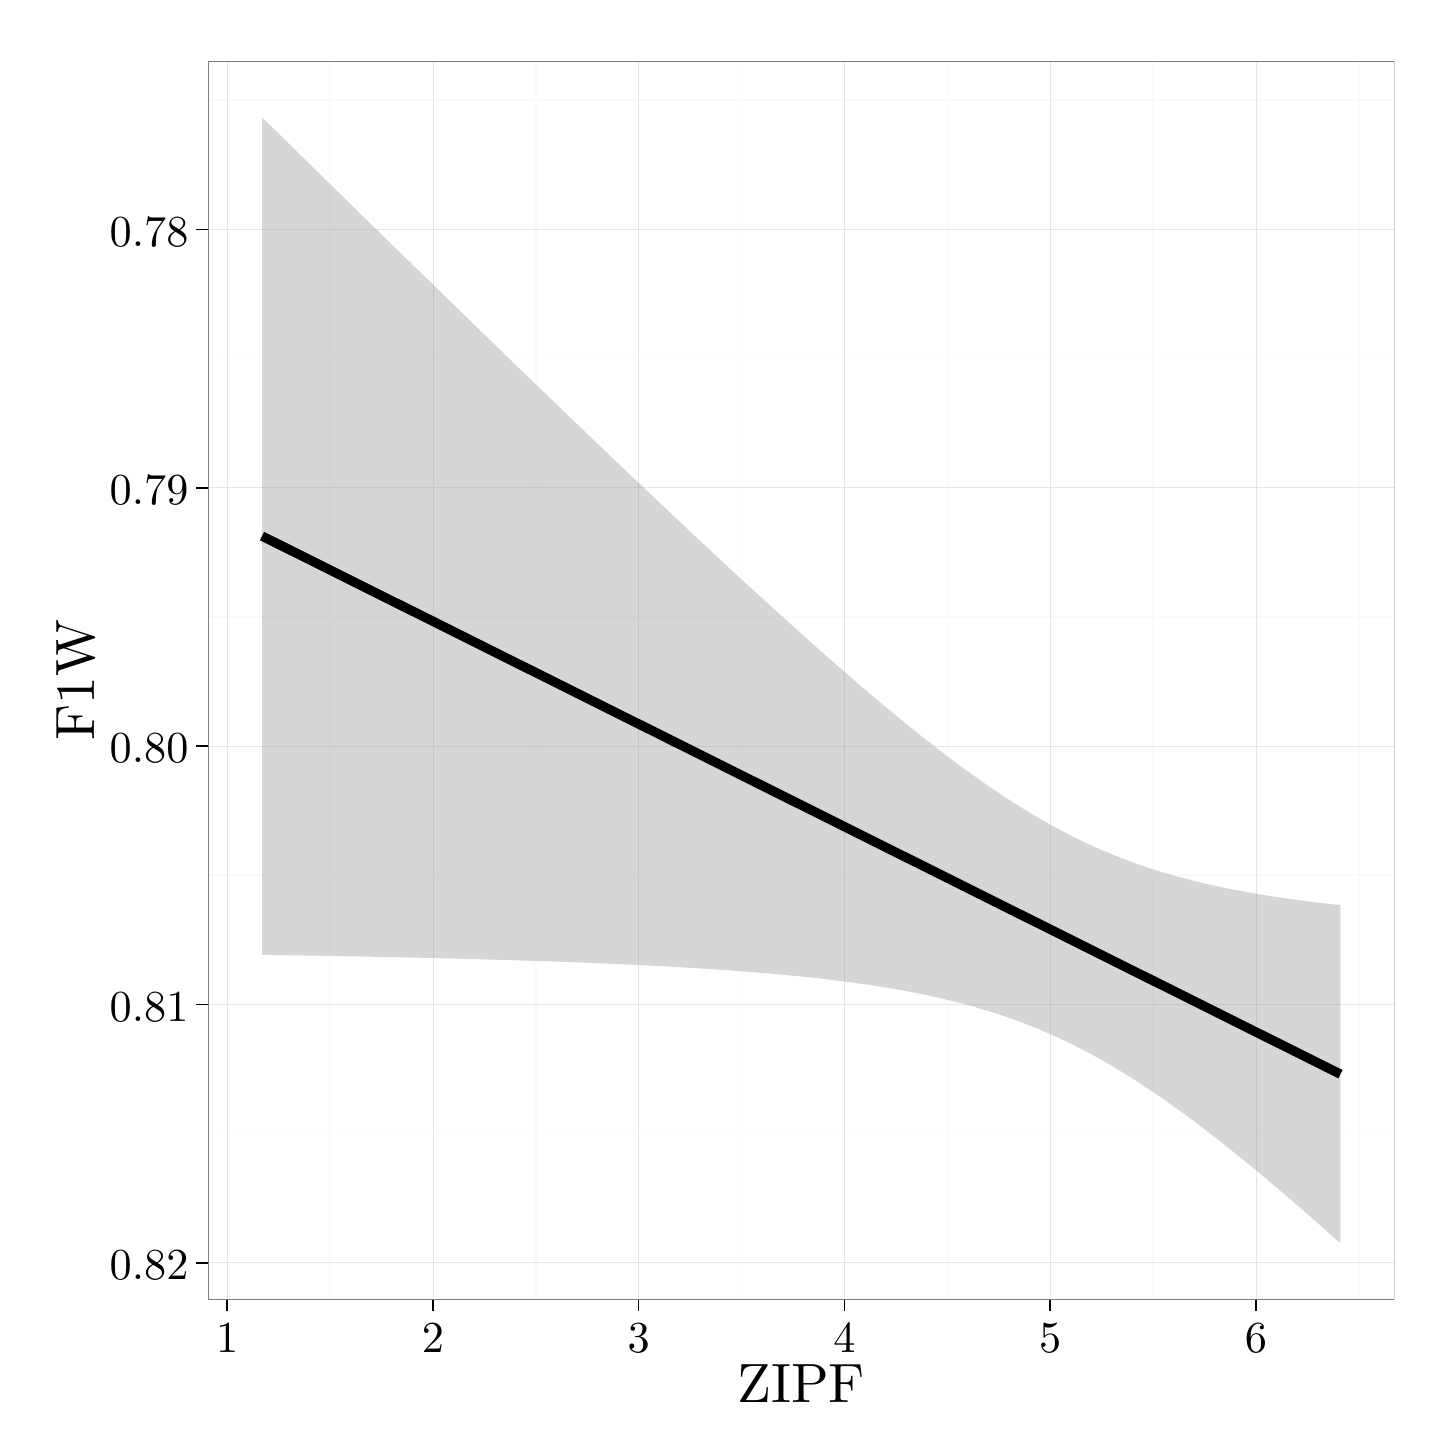
\begin{tikzpicture}[x=1pt,y=1pt]
\definecolor{fillColor}{RGB}{255,255,255}
\path[use as bounding box,fill=fillColor,fill opacity=0.00] (0,0) rectangle (505.89,505.89);
\begin{scope}
\path[clip] (  0.00,  0.00) rectangle (505.89,505.89);
\definecolor{drawColor}{RGB}{255,255,255}
\definecolor{fillColor}{RGB}{255,255,255}

\path[draw=drawColor,line width= 0.6pt,line join=round,line cap=round,fill=fillColor] (  0.00, -0.00) rectangle (505.89,505.89);
\end{scope}
\begin{scope}
\path[clip] ( 65.21, 46.31) rectangle (493.85,493.84);
\definecolor{fillColor}{RGB}{255,255,255}

\path[fill=fillColor] ( 65.21, 46.31) rectangle (493.85,493.84);
\definecolor{drawColor}{gray}{0.98}

\path[draw=drawColor,line width= 0.6pt,line join=round] ( 65.21,479.66) --
	(493.85,479.66);

\path[draw=drawColor,line width= 0.6pt,line join=round] ( 65.21,386.32) --
	(493.85,386.32);

\path[draw=drawColor,line width= 0.6pt,line join=round] ( 65.21,292.97) --
	(493.85,292.97);

\path[draw=drawColor,line width= 0.6pt,line join=round] ( 65.21,199.62) --
	(493.85,199.62);

\path[draw=drawColor,line width= 0.6pt,line join=round] ( 65.21,106.28) --
	(493.85,106.28);

\path[draw=drawColor,line width= 0.6pt,line join=round] (109.24, 46.31) --
	(109.24,493.84);

\path[draw=drawColor,line width= 0.6pt,line join=round] (183.60, 46.31) --
	(183.60,493.84);

\path[draw=drawColor,line width= 0.6pt,line join=round] (257.96, 46.31) --
	(257.96,493.84);

\path[draw=drawColor,line width= 0.6pt,line join=round] (332.33, 46.31) --
	(332.33,493.84);

\path[draw=drawColor,line width= 0.6pt,line join=round] (406.69, 46.31) --
	(406.69,493.84);

\path[draw=drawColor,line width= 0.6pt,line join=round] (481.05, 46.31) --
	(481.05,493.84);
\definecolor{drawColor}{gray}{0.90}

\path[draw=drawColor,line width= 0.2pt,line join=round] ( 65.21,432.99) --
	(493.85,432.99);

\path[draw=drawColor,line width= 0.2pt,line join=round] ( 65.21,339.64) --
	(493.85,339.64);

\path[draw=drawColor,line width= 0.2pt,line join=round] ( 65.21,246.30) --
	(493.85,246.30);

\path[draw=drawColor,line width= 0.2pt,line join=round] ( 65.21,152.95) --
	(493.85,152.95);

\path[draw=drawColor,line width= 0.2pt,line join=round] ( 65.21, 59.60) --
	(493.85, 59.60);

\path[draw=drawColor,line width= 0.2pt,line join=round] ( 72.06, 46.31) --
	( 72.06,493.84);

\path[draw=drawColor,line width= 0.2pt,line join=round] (146.42, 46.31) --
	(146.42,493.84);

\path[draw=drawColor,line width= 0.2pt,line join=round] (220.78, 46.31) --
	(220.78,493.84);

\path[draw=drawColor,line width= 0.2pt,line join=round] (295.15, 46.31) --
	(295.15,493.84);

\path[draw=drawColor,line width= 0.2pt,line join=round] (369.51, 46.31) --
	(369.51,493.84);

\path[draw=drawColor,line width= 0.2pt,line join=round] (443.87, 46.31) --
	(443.87,493.84);
\definecolor{fillColor}{RGB}{153,153,153}

\path[fill=fillColor,fill opacity=0.40] ( 84.70,473.50) --
	( 89.63,468.65) --
	( 94.56,463.81) --
	( 99.49,458.97) --
	(104.43,454.13) --
	(109.36,449.29) --
	(114.29,444.46) --
	(119.22,439.63) --
	(124.16,434.80) --
	(129.09,429.98) --
	(134.02,425.16) --
	(138.95,420.35) --
	(143.89,415.54) --
	(148.82,410.73) --
	(153.75,405.93) --
	(158.68,401.14) --
	(163.62,396.35) --
	(168.55,391.56) --
	(173.48,386.79) --
	(178.41,382.02) --
	(183.35,377.25) --
	(188.28,372.50) --
	(193.21,367.75) --
	(198.14,363.01) --
	(203.08,358.28) --
	(208.01,353.56) --
	(212.94,348.85) --
	(217.87,344.15) --
	(222.81,339.46) --
	(227.74,334.79) --
	(232.67,330.13) --
	(237.60,325.49) --
	(242.54,320.87) --
	(247.47,316.26) --
	(252.40,311.68) --
	(257.33,307.11) --
	(262.27,302.57) --
	(267.20,298.06) --
	(272.13,293.57) --
	(277.06,289.12) --
	(282.00,284.70) --
	(286.93,280.32) --
	(291.86,275.98) --
	(296.79,271.68) --
	(301.73,267.44) --
	(306.66,263.25) --
	(311.59,259.13) --
	(316.52,255.07) --
	(321.46,251.09) --
	(326.39,247.19) --
	(331.32,243.38) --
	(336.25,239.67) --
	(341.19,236.07) --
	(346.12,232.58) --
	(351.05,229.23) --
	(355.98,226.00) --
	(360.92,222.92) --
	(365.85,219.99) --
	(370.78,217.21) --
	(375.71,214.60) --
	(380.64,212.14) --
	(385.58,209.85) --
	(390.51,207.71) --
	(395.44,205.73) --
	(400.37,203.90) --
	(405.31,202.21) --
	(410.24,200.65) --
	(415.17,199.22) --
	(420.10,197.91) --
	(425.04,196.70) --
	(429.97,195.59) --
	(434.90,194.58) --
	(439.83,193.64) --
	(444.77,192.78) --
	(449.70,191.99) --
	(454.63,191.25) --
	(459.56,190.58) --
	(464.50,189.95) --
	(469.43,189.37) --
	(474.36,188.83) --
	(474.36, 66.65) --
	(469.43, 71.03) --
	(464.50, 75.38) --
	(459.56, 79.67) --
	(454.63, 83.92) --
	(449.70, 88.11) --
	(444.77, 92.24) --
	(439.83, 96.30) --
	(434.90,100.29) --
	(429.97,104.19) --
	(425.04,108.01) --
	(420.10,111.73) --
	(415.17,115.33) --
	(410.24,118.83) --
	(405.31,122.19) --
	(400.37,125.43) --
	(395.44,128.52) --
	(390.51,131.46) --
	(385.58,134.25) --
	(380.64,136.87) --
	(375.71,139.34) --
	(370.78,141.64) --
	(365.85,143.79) --
	(360.92,145.78) --
	(355.98,147.62) --
	(351.05,149.32) --
	(346.12,150.89) --
	(341.19,152.32) --
	(336.25,153.65) --
	(331.32,154.86) --
	(326.39,155.97) --
	(321.46,156.99) --
	(316.52,157.94) --
	(311.59,158.80) --
	(306.66,159.60) --
	(301.73,160.33) --
	(296.79,161.01) --
	(291.86,161.64) --
	(286.93,162.23) --
	(282.00,162.77) --
	(277.06,163.27) --
	(272.13,163.74) --
	(267.20,164.18) --
	(262.27,164.58) --
	(257.33,164.97) --
	(252.40,165.32) --
	(247.47,165.66) --
	(242.54,165.98) --
	(237.60,166.27) --
	(232.67,166.56) --
	(227.74,166.82) --
	(222.81,167.07) --
	(217.87,167.31) --
	(212.94,167.53) --
	(208.01,167.75) --
	(203.08,167.95) --
	(198.14,168.14) --
	(193.21,168.32) --
	(188.28,168.50) --
	(183.35,168.66) --
	(178.41,168.82) --
	(173.48,168.97) --
	(168.55,169.12) --
	(163.62,169.26) --
	(158.68,169.39) --
	(153.75,169.52) --
	(148.82,169.64) --
	(143.89,169.76) --
	(138.95,169.87) --
	(134.02,169.98) --
	(129.09,170.08) --
	(124.16,170.18) --
	(119.22,170.28) --
	(114.29,170.37) --
	(109.36,170.46) --
	(104.43,170.55) --
	( 99.49,170.63) --
	( 94.56,170.71) --
	( 89.63,170.79) --
	( 84.70,170.86) --
	cycle;
\definecolor{drawColor}{RGB}{0,0,0}

\path[draw=drawColor,line width= 3.4pt,line join=round] ( 84.70,322.18) --
	( 89.63,319.72) --
	( 94.56,317.26) --
	( 99.49,314.80) --
	(104.43,312.34) --
	(109.36,309.88) --
	(114.29,307.42) --
	(119.22,304.95) --
	(124.16,302.49) --
	(129.09,300.03) --
	(134.02,297.57) --
	(138.95,295.11) --
	(143.89,292.65) --
	(148.82,290.19) --
	(153.75,287.73) --
	(158.68,285.26) --
	(163.62,282.80) --
	(168.55,280.34) --
	(173.48,277.88) --
	(178.41,275.42) --
	(183.35,272.96) --
	(188.28,270.50) --
	(193.21,268.04) --
	(198.14,265.57) --
	(203.08,263.11) --
	(208.01,260.65) --
	(212.94,258.19) --
	(217.87,255.73) --
	(222.81,253.27) --
	(227.74,250.81) --
	(232.67,248.34) --
	(237.60,245.88) --
	(242.54,243.42) --
	(247.47,240.96) --
	(252.40,238.50) --
	(257.33,236.04) --
	(262.27,233.58) --
	(267.20,231.12) --
	(272.13,228.65) --
	(277.06,226.19) --
	(282.00,223.73) --
	(286.93,221.27) --
	(291.86,218.81) --
	(296.79,216.35) --
	(301.73,213.89) --
	(306.66,211.43) --
	(311.59,208.96) --
	(316.52,206.50) --
	(321.46,204.04) --
	(326.39,201.58) --
	(331.32,199.12) --
	(336.25,196.66) --
	(341.19,194.20) --
	(346.12,191.74) --
	(351.05,189.27) --
	(355.98,186.81) --
	(360.92,184.35) --
	(365.85,181.89) --
	(370.78,179.43) --
	(375.71,176.97) --
	(380.64,174.51) --
	(385.58,172.05) --
	(390.51,169.58) --
	(395.44,167.12) --
	(400.37,164.66) --
	(405.31,162.20) --
	(410.24,159.74) --
	(415.17,157.28) --
	(420.10,154.82) --
	(425.04,152.36) --
	(429.97,149.89) --
	(434.90,147.43) --
	(439.83,144.97) --
	(444.77,142.51) --
	(449.70,140.05) --
	(454.63,137.59) --
	(459.56,135.13) --
	(464.50,132.66) --
	(469.43,130.20) --
	(474.36,127.74);
\definecolor{drawColor}{gray}{0.50}

\path[draw=drawColor,line width= 0.6pt,line join=round,line cap=round] ( 65.21, 46.31) rectangle (493.85,493.84);
\end{scope}
\begin{scope}
\path[clip] (  0.00,  0.00) rectangle (505.89,505.89);
\definecolor{drawColor}{RGB}{0,0,0}

\node[text=drawColor,anchor=base east,inner sep=0pt, outer sep=0pt, scale=  1.60] at ( 58.10,426.96) {0.78};

\node[text=drawColor,anchor=base east,inner sep=0pt, outer sep=0pt, scale=  1.60] at ( 58.10,333.61) {0.79};

\node[text=drawColor,anchor=base east,inner sep=0pt, outer sep=0pt, scale=  1.60] at ( 58.10,240.26) {0.80};

\node[text=drawColor,anchor=base east,inner sep=0pt, outer sep=0pt, scale=  1.60] at ( 58.10,146.92) {0.81};

\node[text=drawColor,anchor=base east,inner sep=0pt, outer sep=0pt, scale=  1.60] at ( 58.10, 53.57) {0.82};
\end{scope}
\begin{scope}
\path[clip] (  0.00,  0.00) rectangle (505.89,505.89);
\definecolor{drawColor}{RGB}{0,0,0}

\path[draw=drawColor,line width= 0.6pt,line join=round] ( 60.95,432.99) --
	( 65.21,432.99);

\path[draw=drawColor,line width= 0.6pt,line join=round] ( 60.95,339.64) --
	( 65.21,339.64);

\path[draw=drawColor,line width= 0.6pt,line join=round] ( 60.95,246.30) --
	( 65.21,246.30);

\path[draw=drawColor,line width= 0.6pt,line join=round] ( 60.95,152.95) --
	( 65.21,152.95);

\path[draw=drawColor,line width= 0.6pt,line join=round] ( 60.95, 59.60) --
	( 65.21, 59.60);
\end{scope}
\begin{scope}
\path[clip] (  0.00,  0.00) rectangle (505.89,505.89);
\definecolor{drawColor}{RGB}{0,0,0}

\path[draw=drawColor,line width= 0.6pt,line join=round] ( 72.06, 42.04) --
	( 72.06, 46.31);

\path[draw=drawColor,line width= 0.6pt,line join=round] (146.42, 42.04) --
	(146.42, 46.31);

\path[draw=drawColor,line width= 0.6pt,line join=round] (220.78, 42.04) --
	(220.78, 46.31);

\path[draw=drawColor,line width= 0.6pt,line join=round] (295.15, 42.04) --
	(295.15, 46.31);

\path[draw=drawColor,line width= 0.6pt,line join=round] (369.51, 42.04) --
	(369.51, 46.31);

\path[draw=drawColor,line width= 0.6pt,line join=round] (443.87, 42.04) --
	(443.87, 46.31);
\end{scope}
\begin{scope}
\path[clip] (  0.00,  0.00) rectangle (505.89,505.89);
\definecolor{drawColor}{RGB}{0,0,0}

\node[text=drawColor,anchor=base,inner sep=0pt, outer sep=0pt, scale=  1.60] at ( 72.06, 27.13) {1};

\node[text=drawColor,anchor=base,inner sep=0pt, outer sep=0pt, scale=  1.60] at (146.42, 27.13) {2};

\node[text=drawColor,anchor=base,inner sep=0pt, outer sep=0pt, scale=  1.60] at (220.78, 27.13) {3};

\node[text=drawColor,anchor=base,inner sep=0pt, outer sep=0pt, scale=  1.60] at (295.15, 27.13) {4};

\node[text=drawColor,anchor=base,inner sep=0pt, outer sep=0pt, scale=  1.60] at (369.51, 27.13) {5};

\node[text=drawColor,anchor=base,inner sep=0pt, outer sep=0pt, scale=  1.60] at (443.87, 27.13) {6};
\end{scope}
\begin{scope}
\path[clip] (  0.00,  0.00) rectangle (505.89,505.89);
\definecolor{drawColor}{RGB}{0,0,0}

\node[text=drawColor,anchor=base,inner sep=0pt, outer sep=0pt, scale=  2.00] at (279.53,  9.03) {ZIPF};
\end{scope}
\begin{scope}
\path[clip] (  0.00,  0.00) rectangle (505.89,505.89);
\definecolor{drawColor}{RGB}{0,0,0}

\node[text=drawColor,rotate= 90.00,anchor=base,inner sep=0pt, outer sep=0pt, scale=  2.00] at ( 24.12,270.08) {F1W};
\end{scope}
\end{tikzpicture}
}
		\caption{happ\textsc{y} (F1) by frequency of carrier word}
		\label{fig.scatter.f1w.happy.zipf}
	\end{figure}

Despite the fact that it is only a statistical trend we will also briefly look at the impact of \isi{frequency} on F1 values in another regression plot.
If one considers the scales of the y-axes in Figures \ref{fig.scatter.f1w.happy.dur} and \ref{fig.scatter.f1w.happy.zipf} it becomes immediately obvious that both \isi{frequency} and duration\is{vowel duration} have only a rather small influence on F1.
Higher Zipf\is{Zipf score} scores on the x-axis indicate more frequent carrier words, so the bottom line of this graph is that the more frequent a word containing happ\textsc{y} is, the lower the realisation of happ\textsc{y} will be --- which is something that is also implied by the positive correlation coefficient in the mixed-effects model.
This is in line with what we know about \isi{frequency} effects in general, viz. that higher frequencies of use favour phonetic reduction processes.
It should be borne in mind, however, that my sample is based on spoken and relatively informal language, and therefore consists almost exclusively of high \isi{frequency} words, anyway (Zipf\is{Zipf score} scores for happ\textsc{y} carrier words: mean = 5.114, first quantile = 4.57, median = 5.37, third quantile = 5.79).
Data on low \isi{frequency} words are comparatively scarce, which also shows in the larger standard deviation for these tokens (cf. the larger dark grey area on the left-hand side of Figure \ref{fig.scatter.f1w.happy.zipf}).
It would be interesting to see if the tendency described above would also surface (possibly in a statistically more robust way) in a sample that is more balanced in this respect.

			\subsubsection{Class and gender}
			\label{sec.prod.res.vow.happy.f1.classgender}

We will now turn towards the first social predictor, class of speaker.
The mixed-effects regression model found a positive correlation coefficient for middle-class interviewees.
This highly significant correlation indicates that middle-class speakers produced lower happ\textsc{y} realisations (higher F1 values) than their working-class counterparts.
This in itself is interesting (and somewhat unexpected), but instead of going into this class difference by itself, I would like to immediately include the significant interaction of social class and gender that the mixed-effects model revealed as well.
Said interaction is visualised in Figures \ref{fig.box.f1w.happy.genderclass} and \ref{fig.scatter.f1w.happy.genderclass}.

	\begin{figure}[h!]
		\centering
		\begin{subfigure}{.49\textwidth}
			\centering
			\definecolor{shadecolor}{rgb}{0.969, 0.969, 0.969}
			\resizebox{\linewidth}{!}{% Created by tikzDevice version 0.8.1 on 2016-02-09 02:12:27
% !TEX encoding = UTF-8 Unicode
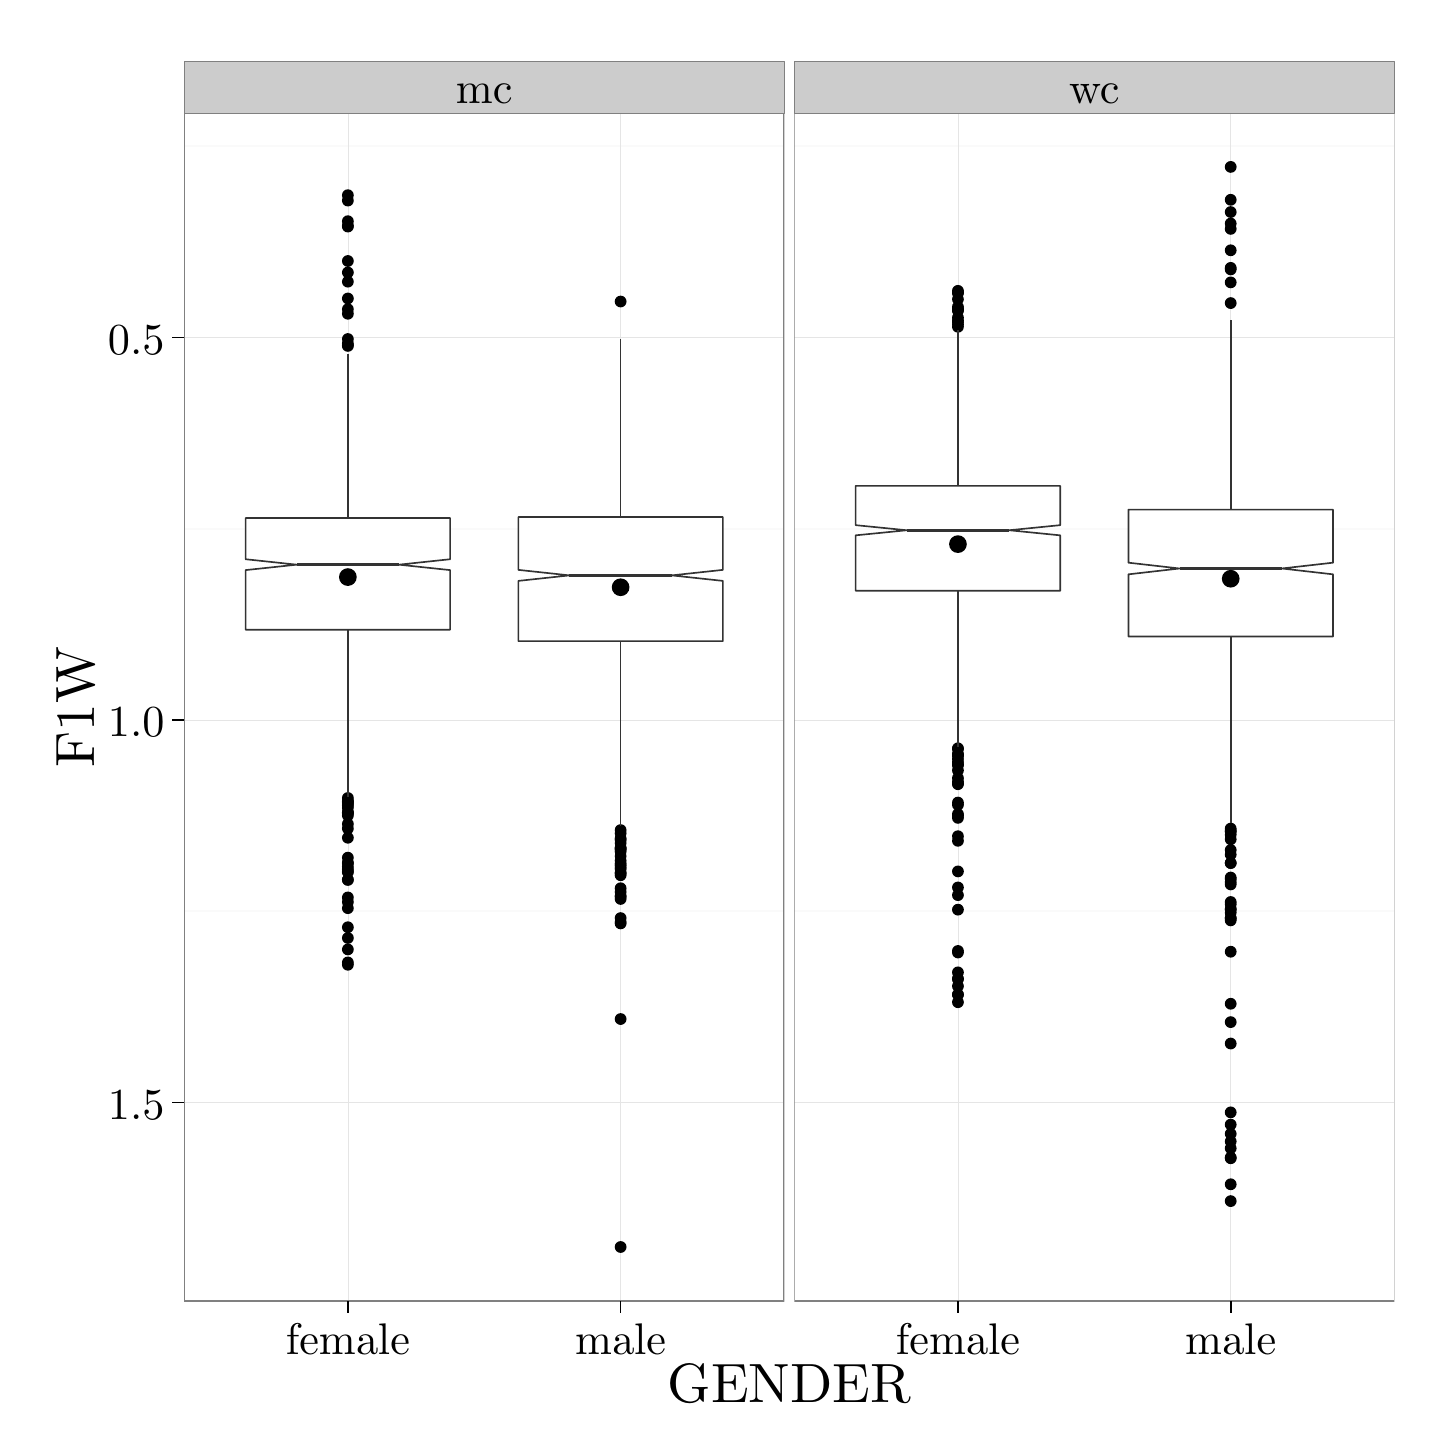
\begin{tikzpicture}[x=1pt,y=1pt]
\definecolor{fillColor}{RGB}{255,255,255}
\path[use as bounding box,fill=fillColor,fill opacity=0.00] (0,0) rectangle (505.89,505.89);
\begin{scope}
\path[clip] (  0.00,  0.00) rectangle (505.89,505.89);
\definecolor{drawColor}{RGB}{255,255,255}
\definecolor{fillColor}{RGB}{255,255,255}

\path[draw=drawColor,line width= 0.6pt,line join=round,line cap=round,fill=fillColor] (  0.00, -0.00) rectangle (505.89,505.89);
\end{scope}
\begin{scope}
\path[clip] ( 56.56, 45.77) rectangle (273.40,475.09);
\definecolor{fillColor}{RGB}{255,255,255}

\path[fill=fillColor] ( 56.56, 45.77) rectangle (273.40,475.09);
\definecolor{drawColor}{gray}{0.98}

\path[draw=drawColor,line width= 0.6pt,line join=round] ( 56.56,463.04) --
	(273.40,463.04);

\path[draw=drawColor,line width= 0.6pt,line join=round] ( 56.56,324.83) --
	(273.40,324.83);

\path[draw=drawColor,line width= 0.6pt,line join=round] ( 56.56,186.63) --
	(273.40,186.63);
\definecolor{drawColor}{gray}{0.90}

\path[draw=drawColor,line width= 0.2pt,line join=round] ( 56.56,393.93) --
	(273.40,393.93);

\path[draw=drawColor,line width= 0.2pt,line join=round] ( 56.56,255.73) --
	(273.40,255.73);

\path[draw=drawColor,line width= 0.2pt,line join=round] ( 56.56,117.53) --
	(273.40,117.53);

\path[draw=drawColor,line width= 0.2pt,line join=round] (115.70, 45.77) --
	(115.70,475.09);

\path[draw=drawColor,line width= 0.2pt,line join=round] (214.26, 45.77) --
	(214.26,475.09);
\definecolor{fillColor}{RGB}{0,0,0}

\path[fill=fillColor] (115.70,204.04) circle (  2.13);

\path[fill=fillColor] (115.70,189.95) circle (  2.13);

\path[fill=fillColor] (115.70,223.94) circle (  2.13);

\path[fill=fillColor] (115.70,402.50) circle (  2.13);

\path[fill=fillColor] (115.70,226.16) circle (  2.13);

\path[fill=fillColor] (115.70,226.43) circle (  2.13);

\path[fill=fillColor] (115.70,221.18) circle (  2.13);

\path[fill=fillColor] (115.70,391.72) circle (  2.13);

\path[fill=fillColor] (115.70,421.57) circle (  2.13);

\path[fill=fillColor] (115.70,445.35) circle (  2.13);

\path[fill=fillColor] (115.70,404.16) circle (  2.13);

\path[fill=fillColor] (115.70,435.95) circle (  2.13);

\path[fill=fillColor] (115.70,434.29) circle (  2.13);

\path[fill=fillColor] (115.70,443.41) circle (  2.13);

\path[fill=fillColor] (115.70,414.11) circle (  2.13);

\path[fill=fillColor] (115.70,417.43) circle (  2.13);

\path[fill=fillColor] (115.70,408.03) circle (  2.13);

\path[fill=fillColor] (115.70,391.17) circle (  2.13);

\path[fill=fillColor] (115.70,225.88) circle (  2.13);

\path[fill=fillColor] (115.70,176.95) circle (  2.13);

\path[fill=fillColor] (115.70,172.81) circle (  2.13);

\path[fill=fillColor] (115.70,187.73) circle (  2.13);

\path[fill=fillColor] (115.70,202.66) circle (  2.13);

\path[fill=fillColor] (115.70,224.77) circle (  2.13);

\path[fill=fillColor] (115.70,222.01) circle (  2.13);

\path[fill=fillColor] (115.70,201.83) circle (  2.13);

\path[fill=fillColor] (115.70,218.14) circle (  2.13);

\path[fill=fillColor] (115.70,204.04) circle (  2.13);

\path[fill=fillColor] (115.70,191.60) circle (  2.13);

\path[fill=fillColor] (115.70,180.82) circle (  2.13);

\path[fill=fillColor] (115.70,201.00) circle (  2.13);

\path[fill=fillColor] (115.70,213.16) circle (  2.13);

\path[fill=fillColor] (115.70,168.11) circle (  2.13);

\path[fill=fillColor] (115.70,167.28) circle (  2.13);

\path[fill=fillColor] (115.70,393.38) circle (  2.13);

\path[fill=fillColor] (115.70,197.96) circle (  2.13);

\path[fill=fillColor] (115.70,200.73) circle (  2.13);

\path[fill=fillColor] (115.70,434.01) circle (  2.13);

\path[fill=fillColor] (115.70,222.29) circle (  2.13);

\path[fill=fillColor] (115.70,205.98) circle (  2.13);

\path[fill=fillColor] (115.70,216.48) circle (  2.13);

\path[fill=fillColor] (115.70,225.33) circle (  2.13);

\path[fill=fillColor] (115.70,227.54) circle (  2.13);

\path[fill=fillColor] (115.70,197.96) circle (  2.13);

\path[fill=fillColor] (115.70,222.29) circle (  2.13);

\path[fill=fillColor] (115.70,390.89) circle (  2.13);
\definecolor{drawColor}{gray}{0.20}

\path[draw=drawColor,line width= 0.6pt,line join=round] (115.70,328.70) -- (115.70,387.85);

\path[draw=drawColor,line width= 0.6pt,line join=round] (115.70,288.35) -- (115.70,227.81);
\definecolor{fillColor}{RGB}{255,255,255}

\path[draw=drawColor,line width= 0.6pt,line join=round,line cap=round,fill=fillColor] ( 78.74,328.70) --
	( 78.74,313.81) --
	( 97.22,311.84) --
	( 78.74,309.88) --
	( 78.74,288.35) --
	(152.66,288.35) --
	(152.66,309.88) --
	(134.18,311.84) --
	(152.66,313.81) --
	(152.66,328.70) --
	( 78.74,328.70) --
	cycle;

\path[draw=drawColor,line width= 1.1pt,line join=round] ( 97.22,311.84) -- (134.18,311.84);
\definecolor{fillColor}{RGB}{0,0,0}

\path[fill=fillColor] (214.26,202.38) circle (  2.13);

\path[fill=fillColor] (214.26,200.45) circle (  2.13);

\path[fill=fillColor] (214.26,193.54) circle (  2.13);

\path[fill=fillColor] (214.26,204.87) circle (  2.13);

\path[fill=fillColor] (214.26,147.66) circle (  2.13);

\path[fill=fillColor] (214.26,206.53) circle (  2.13);

\path[fill=fillColor] (214.26,211.23) circle (  2.13);

\path[fill=fillColor] (214.26,194.92) circle (  2.13);

\path[fill=fillColor] (214.26,208.19) circle (  2.13);

\path[fill=fillColor] (214.26,191.88) circle (  2.13);

\path[fill=fillColor] (214.26,201.83) circle (  2.13);

\path[fill=fillColor] (214.26,209.02) circle (  2.13);

\path[fill=fillColor] (214.26,209.57) circle (  2.13);

\path[fill=fillColor] (214.26,209.29) circle (  2.13);

\path[fill=fillColor] (214.26,215.93) circle (  2.13);

\path[fill=fillColor] (214.26,200.45) circle (  2.13);

\path[fill=fillColor] (214.26,212.89) circle (  2.13);

\path[fill=fillColor] (214.26,199.62) circle (  2.13);

\path[fill=fillColor] (214.26,212.33) circle (  2.13);

\path[fill=fillColor] (214.26, 65.29) circle (  2.13);

\path[fill=fillColor] (214.26,191.05) circle (  2.13);

\path[fill=fillColor] (214.26,182.76) circle (  2.13);

\path[fill=fillColor] (214.26,182.21) circle (  2.13);

\path[fill=fillColor] (214.26,406.93) circle (  2.13);

\path[fill=fillColor] (214.26,203.21) circle (  2.13);

\path[fill=fillColor] (214.26,214.82) circle (  2.13);

\path[fill=fillColor] (214.26,184.14) circle (  2.13);

\path[fill=fillColor] (214.26,192.16) circle (  2.13);

\path[fill=fillColor] (214.26,203.77) circle (  2.13);

\path[draw=drawColor,line width= 0.6pt,line join=round] (214.26,329.05) -- (214.26,393.38);

\path[draw=drawColor,line width= 0.6pt,line join=round] (214.26,284.20) -- (214.26,217.31);
\definecolor{fillColor}{RGB}{255,255,255}

\path[draw=drawColor,line width= 0.6pt,line join=round,line cap=round,fill=fillColor] (177.30,329.05) --
	(177.30,309.96) --
	(195.78,307.97) --
	(177.30,305.98) --
	(177.30,284.20) --
	(251.22,284.20) --
	(251.22,305.98) --
	(232.74,307.97) --
	(251.22,309.96) --
	(251.22,329.05) --
	(177.30,329.05) --
	cycle;

\path[draw=drawColor,line width= 1.1pt,line join=round] (195.78,307.97) -- (232.74,307.97);
\definecolor{fillColor}{RGB}{0,0,0}

\path[fill=fillColor] (115.70,307.36) circle (  3.20);

\path[fill=fillColor] (214.26,303.68) circle (  3.20);
\definecolor{drawColor}{gray}{0.50}

\path[draw=drawColor,line width= 0.6pt,line join=round,line cap=round] ( 56.56, 45.77) rectangle (273.40,475.09);
\end{scope}
\begin{scope}
\path[clip] (277.01, 45.77) rectangle (493.85,475.09);
\definecolor{fillColor}{RGB}{255,255,255}

\path[fill=fillColor] (277.01, 45.77) rectangle (493.85,475.09);
\definecolor{drawColor}{gray}{0.98}

\path[draw=drawColor,line width= 0.6pt,line join=round] (277.01,463.04) --
	(493.85,463.04);

\path[draw=drawColor,line width= 0.6pt,line join=round] (277.01,324.83) --
	(493.85,324.83);

\path[draw=drawColor,line width= 0.6pt,line join=round] (277.01,186.63) --
	(493.85,186.63);
\definecolor{drawColor}{gray}{0.90}

\path[draw=drawColor,line width= 0.2pt,line join=round] (277.01,393.93) --
	(493.85,393.93);

\path[draw=drawColor,line width= 0.2pt,line join=round] (277.01,255.73) --
	(493.85,255.73);

\path[draw=drawColor,line width= 0.2pt,line join=round] (277.01,117.53) --
	(493.85,117.53);

\path[draw=drawColor,line width= 0.2pt,line join=round] (336.15, 45.77) --
	(336.15,475.09);

\path[draw=drawColor,line width= 0.2pt,line join=round] (434.71, 45.77) --
	(434.71,475.09);
\definecolor{fillColor}{RGB}{0,0,0}

\path[fill=fillColor] (336.15,403.61) circle (  2.13);

\path[fill=fillColor] (336.15,401.12) circle (  2.13);

\path[fill=fillColor] (336.15,240.53) circle (  2.13);

\path[fill=fillColor] (336.15,239.70) circle (  2.13);

\path[fill=fillColor] (336.15,403.88) circle (  2.13);

\path[fill=fillColor] (336.15,162.03) circle (  2.13);

\path[fill=fillColor] (336.15,156.50) circle (  2.13);

\path[fill=fillColor] (336.15,409.97) circle (  2.13);

\path[fill=fillColor] (336.15,212.06) circle (  2.13);

\path[fill=fillColor] (336.15,192.43) circle (  2.13);

\path[fill=fillColor] (336.15,399.46) circle (  2.13);

\path[fill=fillColor] (336.15,404.16) circle (  2.13);

\path[fill=fillColor] (336.15,397.80) circle (  2.13);

\path[fill=fillColor] (336.15,159.54) circle (  2.13);

\path[fill=fillColor] (336.15,220.35) circle (  2.13);

\path[fill=fillColor] (336.15,172.26) circle (  2.13);

\path[fill=fillColor] (336.15,404.99) circle (  2.13);

\path[fill=fillColor] (336.15,241.63) circle (  2.13);

\path[fill=fillColor] (336.15,239.42) circle (  2.13);

\path[fill=fillColor] (336.15,164.52) circle (  2.13);

\path[fill=fillColor] (336.15,398.63) circle (  2.13);

\path[fill=fillColor] (336.15,233.34) circle (  2.13);

\path[fill=fillColor] (336.15,195.20) circle (  2.13);

\path[fill=fillColor] (336.15,232.51) circle (  2.13);

\path[fill=fillColor] (336.15,410.79) circle (  2.13);

\path[fill=fillColor] (336.15,201.00) circle (  2.13);

\path[fill=fillColor] (336.15,407.75) circle (  2.13);

\path[fill=fillColor] (336.15,225.05) circle (  2.13);

\path[fill=fillColor] (336.15,410.24) circle (  2.13);

\path[fill=fillColor] (336.15,213.72) circle (  2.13);

\path[fill=fillColor] (336.15,243.29) circle (  2.13);

\path[fill=fillColor] (336.15,153.74) circle (  2.13);

\path[fill=fillColor] (336.15,221.18) circle (  2.13);

\path[fill=fillColor] (336.15,400.01) circle (  2.13);

\path[fill=fillColor] (336.15,171.70) circle (  2.13);

\path[fill=fillColor] (336.15,156.50) circle (  2.13);

\path[fill=fillColor] (336.15,162.31) circle (  2.13);

\path[fill=fillColor] (336.15,234.72) circle (  2.13);

\path[fill=fillColor] (336.15,245.50) circle (  2.13);

\path[fill=fillColor] (336.15,237.49) circle (  2.13);

\path[fill=fillColor] (336.15,232.79) circle (  2.13);

\path[fill=fillColor] (336.15,225.88) circle (  2.13);

\path[fill=fillColor] (336.15,187.18) circle (  2.13);

\path[fill=fillColor] (336.15,221.73) circle (  2.13);

\path[fill=fillColor] (336.15,243.29) circle (  2.13);

\path[fill=fillColor] (336.15,245.23) circle (  2.13);

\path[fill=fillColor] (336.15,242.74) circle (  2.13);
\definecolor{drawColor}{gray}{0.20}

\path[draw=drawColor,line width= 0.6pt,line join=round] (336.15,340.31) -- (336.15,396.70);

\path[draw=drawColor,line width= 0.6pt,line join=round] (336.15,302.44) -- (336.15,246.06);
\definecolor{fillColor}{RGB}{255,255,255}

\path[draw=drawColor,line width= 0.6pt,line join=round,line cap=round,fill=fillColor] (299.19,340.31) --
	(299.19,326.12) --
	(317.67,324.28) --
	(299.19,322.44) --
	(299.19,302.44) --
	(373.11,302.44) --
	(373.11,322.44) --
	(354.63,324.28) --
	(373.11,326.12) --
	(373.11,340.31) --
	(299.19,340.31) --
	cycle;

\path[draw=drawColor,line width= 1.1pt,line join=round] (317.67,324.28) -- (354.63,324.28);
\definecolor{fillColor}{RGB}{0,0,0}

\path[fill=fillColor] (434.71,433.18) circle (  2.13);

\path[fill=fillColor] (434.71,197.13) circle (  2.13);

\path[fill=fillColor] (434.71,455.57) circle (  2.13);

\path[fill=fillColor] (434.71,187.18) circle (  2.13);

\path[fill=fillColor] (434.71,198.79) circle (  2.13);

\path[fill=fillColor] (434.71,419.09) circle (  2.13);

\path[fill=fillColor] (434.71,183.31) circle (  2.13);

\path[fill=fillColor] (434.71,406.37) circle (  2.13);

\path[fill=fillColor] (434.71,208.74) circle (  2.13);

\path[fill=fillColor] (434.71,196.30) circle (  2.13);

\path[fill=fillColor] (434.71,435.12) circle (  2.13);

\path[fill=fillColor] (434.71,215.65) circle (  2.13);

\path[fill=fillColor] (434.71,184.14) circle (  2.13);

\path[fill=fillColor] (434.71,204.04) circle (  2.13);

\path[fill=fillColor] (434.71,212.61) circle (  2.13);

\path[fill=fillColor] (434.71,425.44) circle (  2.13);

\path[fill=fillColor] (434.71,439.26) circle (  2.13);

\path[fill=fillColor] (434.71,413.84) circle (  2.13);

\path[fill=fillColor] (434.71,418.53) circle (  2.13);

\path[fill=fillColor] (434.71,153.18) circle (  2.13);

\path[fill=fillColor] (434.71,138.81) circle (  2.13);

\path[fill=fillColor] (434.71,207.08) circle (  2.13);

\path[fill=fillColor] (434.71,186.08) circle (  2.13);

\path[fill=fillColor] (434.71,215.38) circle (  2.13);

\path[fill=fillColor] (434.71,184.14) circle (  2.13);

\path[fill=fillColor] (434.71,214.27) circle (  2.13);

\path[fill=fillColor] (434.71,171.98) circle (  2.13);

\path[fill=fillColor] (434.71,189.12) circle (  2.13);

\path[fill=fillColor] (434.71, 81.87) circle (  2.13);

\path[fill=fillColor] (434.71,198.24) circle (  2.13);

\path[fill=fillColor] (434.71,216.48) circle (  2.13);

\path[fill=fillColor] (434.71,106.19) circle (  2.13);

\path[fill=fillColor] (434.71, 97.63) circle (  2.13);

\path[fill=fillColor] (434.71,146.55) circle (  2.13);

\path[fill=fillColor] (434.71, 87.95) circle (  2.13);

\path[fill=fillColor] (434.71,109.51) circle (  2.13);

\path[fill=fillColor] (434.71,187.46) circle (  2.13);

\path[fill=fillColor] (434.71,443.69) circle (  2.13);

\path[fill=fillColor] (434.71,189.95) circle (  2.13);

\path[fill=fillColor] (434.71,113.93) circle (  2.13);

\path[fill=fillColor] (434.71, 97.35) circle (  2.13);

\path[fill=fillColor] (434.71,103.43) circle (  2.13);

\path[fill=fillColor] (434.71,204.04) circle (  2.13);

\path[fill=fillColor] (434.71,100.94) circle (  2.13);

\path[draw=drawColor,line width= 0.6pt,line join=round] (434.71,331.74) -- (434.71,400.29);

\path[draw=drawColor,line width= 0.6pt,line join=round] (434.71,285.86) -- (434.71,218.42);
\definecolor{fillColor}{RGB}{255,255,255}

\path[draw=drawColor,line width= 0.6pt,line join=round,line cap=round,fill=fillColor] (397.75,331.74) --
	(397.75,312.56) --
	(416.23,310.46) --
	(397.75,308.35) --
	(397.75,285.86) --
	(471.67,285.86) --
	(471.67,308.35) --
	(453.19,310.46) --
	(471.67,312.56) --
	(471.67,331.74) --
	(397.75,331.74) --
	cycle;

\path[draw=drawColor,line width= 1.1pt,line join=round] (416.23,310.46) -- (453.19,310.46);
\definecolor{fillColor}{RGB}{0,0,0}

\path[fill=fillColor] (336.15,319.27) circle (  3.20);

\path[fill=fillColor] (434.71,306.76) circle (  3.20);
\definecolor{drawColor}{gray}{0.50}

\path[draw=drawColor,line width= 0.6pt,line join=round,line cap=round] (277.01, 45.77) rectangle (493.85,475.09);
\end{scope}
\begin{scope}
\path[clip] (  0.00,  0.00) rectangle (505.89,505.89);
\definecolor{drawColor}{gray}{0.50}
\definecolor{fillColor}{gray}{0.80}

\path[draw=drawColor,line width= 0.2pt,line join=round,line cap=round,fill=fillColor] ( 56.56,475.09) rectangle (273.40,493.85);
\definecolor{drawColor}{RGB}{0,0,0}

\node[text=drawColor,anchor=base,inner sep=0pt, outer sep=0pt, scale=  1.60] at (164.98,478.43) {mc};
\end{scope}
\begin{scope}
\path[clip] (  0.00,  0.00) rectangle (505.89,505.89);
\definecolor{drawColor}{gray}{0.50}
\definecolor{fillColor}{gray}{0.80}

\path[draw=drawColor,line width= 0.2pt,line join=round,line cap=round,fill=fillColor] (277.01,475.09) rectangle (493.85,493.85);
\definecolor{drawColor}{RGB}{0,0,0}

\node[text=drawColor,anchor=base,inner sep=0pt, outer sep=0pt, scale=  1.60] at (385.43,478.43) {wc};
\end{scope}
\begin{scope}
\path[clip] (  0.00,  0.00) rectangle (505.89,505.89);
\definecolor{drawColor}{RGB}{0,0,0}

\node[text=drawColor,anchor=base east,inner sep=0pt, outer sep=0pt, scale=  1.60] at ( 49.45,387.90) {0.5};

\node[text=drawColor,anchor=base east,inner sep=0pt, outer sep=0pt, scale=  1.60] at ( 49.45,249.70) {1.0};

\node[text=drawColor,anchor=base east,inner sep=0pt, outer sep=0pt, scale=  1.60] at ( 49.45,111.49) {1.5};
\end{scope}
\begin{scope}
\path[clip] (  0.00,  0.00) rectangle (505.89,505.89);
\definecolor{drawColor}{RGB}{0,0,0}

\path[draw=drawColor,line width= 0.6pt,line join=round] ( 52.30,393.93) --
	( 56.56,393.93);

\path[draw=drawColor,line width= 0.6pt,line join=round] ( 52.30,255.73) --
	( 56.56,255.73);

\path[draw=drawColor,line width= 0.6pt,line join=round] ( 52.30,117.53) --
	( 56.56,117.53);
\end{scope}
\begin{scope}
\path[clip] (  0.00,  0.00) rectangle (505.89,505.89);
\definecolor{drawColor}{RGB}{0,0,0}

\path[draw=drawColor,line width= 0.6pt,line join=round] (115.70, 41.50) --
	(115.70, 45.77);

\path[draw=drawColor,line width= 0.6pt,line join=round] (214.26, 41.50) --
	(214.26, 45.77);
\end{scope}
\begin{scope}
\path[clip] (  0.00,  0.00) rectangle (505.89,505.89);
\definecolor{drawColor}{RGB}{0,0,0}

\node[text=drawColor,anchor=base,inner sep=0pt, outer sep=0pt, scale=  1.60] at (115.70, 26.59) {female};

\node[text=drawColor,anchor=base,inner sep=0pt, outer sep=0pt, scale=  1.60] at (214.26, 26.59) {male};
\end{scope}
\begin{scope}
\path[clip] (  0.00,  0.00) rectangle (505.89,505.89);
\definecolor{drawColor}{RGB}{0,0,0}

\path[draw=drawColor,line width= 0.6pt,line join=round] (336.15, 41.50) --
	(336.15, 45.77);

\path[draw=drawColor,line width= 0.6pt,line join=round] (434.71, 41.50) --
	(434.71, 45.77);
\end{scope}
\begin{scope}
\path[clip] (  0.00,  0.00) rectangle (505.89,505.89);
\definecolor{drawColor}{RGB}{0,0,0}

\node[text=drawColor,anchor=base,inner sep=0pt, outer sep=0pt, scale=  1.60] at (336.15, 26.59) {female};

\node[text=drawColor,anchor=base,inner sep=0pt, outer sep=0pt, scale=  1.60] at (434.71, 26.59) {male};
\end{scope}
\begin{scope}
\path[clip] (  0.00,  0.00) rectangle (505.89,505.89);
\definecolor{drawColor}{RGB}{0,0,0}

\node[text=drawColor,anchor=base,inner sep=0pt, outer sep=0pt, scale=  2.00] at (275.20,  9.03) {GENDER};
\end{scope}
\begin{scope}
\path[clip] (  0.00,  0.00) rectangle (505.89,505.89);
\definecolor{drawColor}{RGB}{0,0,0}

\node[text=drawColor,rotate= 90.00,anchor=base,inner sep=0pt, outer sep=0pt, scale=  2.00] at ( 24.12,260.43) {F1W};
\end{scope}
\end{tikzpicture}
} 
			\caption{box plot}
			\label{fig.box.f1w.happy.genderclass}
		\end{subfigure}
		\begin{subfigure}{.49\textwidth}
			\centering
			\definecolor{shadecolor}{rgb}{0.969, 0.969, 0.969}
			\resizebox{\linewidth}{!}{% Created by tikzDevice version 0.8.1 on 2016-02-09 02:12:38
% !TEX encoding = UTF-8 Unicode
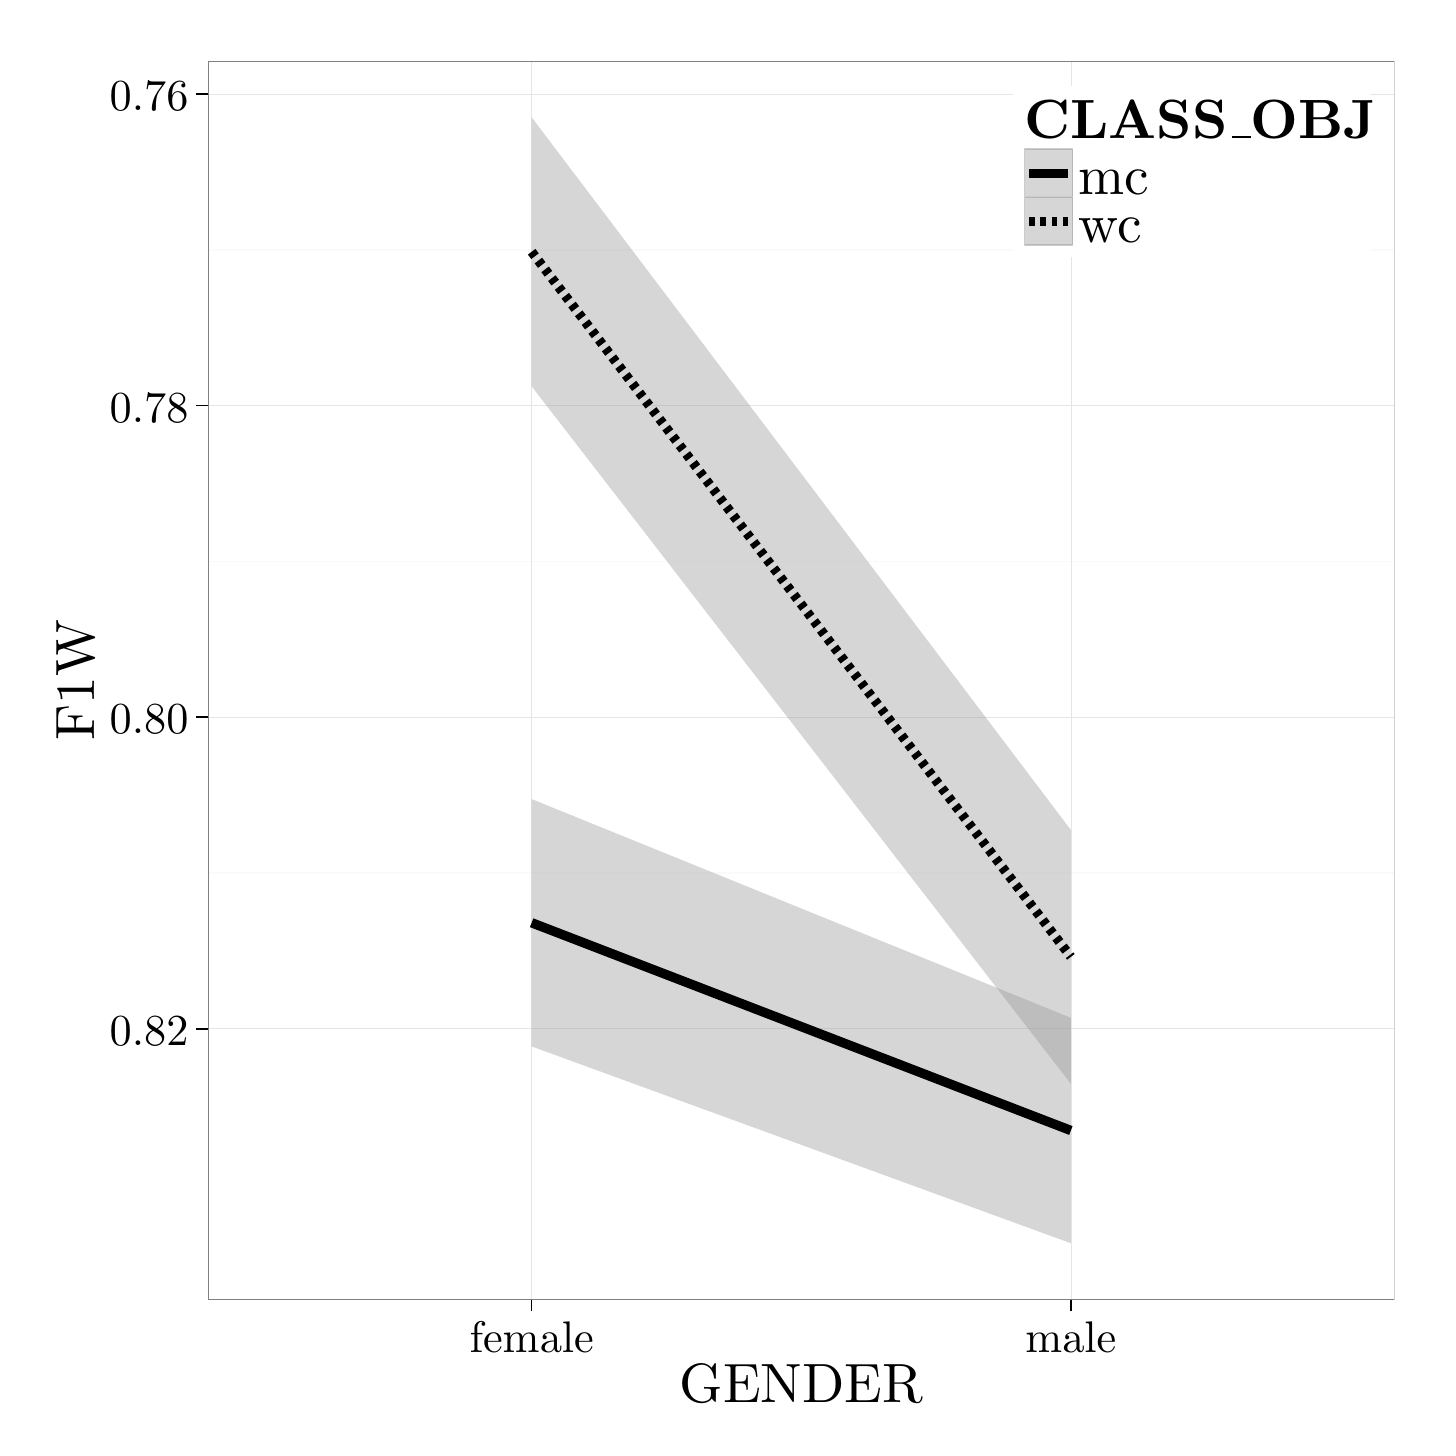
\begin{tikzpicture}[x=1pt,y=1pt]
\definecolor{fillColor}{RGB}{255,255,255}
\path[use as bounding box,fill=fillColor,fill opacity=0.00] (0,0) rectangle (505.89,505.89);
\begin{scope}
\path[clip] (  0.00,  0.00) rectangle (505.89,505.89);
\definecolor{drawColor}{RGB}{255,255,255}
\definecolor{fillColor}{RGB}{255,255,255}

\path[draw=drawColor,line width= 0.6pt,line join=round,line cap=round,fill=fillColor] (  0.00, -0.00) rectangle (505.89,505.89);
\end{scope}
\begin{scope}
\path[clip] ( 65.21, 46.31) rectangle (493.85,493.84);
\definecolor{fillColor}{RGB}{255,255,255}

\path[fill=fillColor] ( 65.21, 46.31) rectangle (493.85,493.84);
\definecolor{drawColor}{gray}{0.98}

\path[draw=drawColor,line width= 0.6pt,line join=round] ( 65.21,425.58) --
	(493.85,425.58);

\path[draw=drawColor,line width= 0.6pt,line join=round] ( 65.21,313.01) --
	(493.85,313.01);

\path[draw=drawColor,line width= 0.6pt,line join=round] ( 65.21,200.45) --
	(493.85,200.45);
\definecolor{drawColor}{gray}{0.90}

\path[draw=drawColor,line width= 0.2pt,line join=round] ( 65.21,481.86) --
	(493.85,481.86);

\path[draw=drawColor,line width= 0.2pt,line join=round] ( 65.21,369.30) --
	(493.85,369.30);

\path[draw=drawColor,line width= 0.2pt,line join=round] ( 65.21,256.73) --
	(493.85,256.73);

\path[draw=drawColor,line width= 0.2pt,line join=round] ( 65.21,144.17) --
	(493.85,144.17);

\path[draw=drawColor,line width= 0.2pt,line join=round] (182.11, 46.31) --
	(182.11,493.84);

\path[draw=drawColor,line width= 0.2pt,line join=round] (376.95, 46.31) --
	(376.95,493.84);
\definecolor{fillColor}{RGB}{153,153,153}

\path[fill=fillColor,fill opacity=0.40] (182.11,227.14) --
	(376.95,148.10) --
	(376.95, 66.65) --
	(182.11,137.76) --
	cycle;
\definecolor{drawColor}{RGB}{0,0,0}

\path[draw=drawColor,line width= 3.4pt,line join=round] (182.11,182.45) --
	(376.95,107.38);

\path[fill=fillColor,fill opacity=0.40] (182.11,473.50) --
	(376.95,215.99) --
	(376.95,124.26) --
	(182.11,376.29) --
	cycle;

\path[draw=drawColor,line width= 3.4pt,dash pattern=on 2pt off 2pt ,line join=round] (182.11,424.90) --
	(376.95,170.12);
\definecolor{drawColor}{gray}{0.50}

\path[draw=drawColor,line width= 0.6pt,line join=round,line cap=round] ( 65.21, 46.31) rectangle (493.85,493.84);
\end{scope}
\begin{scope}
\path[clip] (  0.00,  0.00) rectangle (505.89,505.89);
\definecolor{drawColor}{RGB}{0,0,0}

\node[text=drawColor,anchor=base east,inner sep=0pt, outer sep=0pt, scale=  1.60] at ( 58.10,475.83) {0.76};

\node[text=drawColor,anchor=base east,inner sep=0pt, outer sep=0pt, scale=  1.60] at ( 58.10,363.26) {0.78};

\node[text=drawColor,anchor=base east,inner sep=0pt, outer sep=0pt, scale=  1.60] at ( 58.10,250.70) {0.80};

\node[text=drawColor,anchor=base east,inner sep=0pt, outer sep=0pt, scale=  1.60] at ( 58.10,138.13) {0.82};
\end{scope}
\begin{scope}
\path[clip] (  0.00,  0.00) rectangle (505.89,505.89);
\definecolor{drawColor}{RGB}{0,0,0}

\path[draw=drawColor,line width= 0.6pt,line join=round] ( 60.95,481.86) --
	( 65.21,481.86);

\path[draw=drawColor,line width= 0.6pt,line join=round] ( 60.95,369.30) --
	( 65.21,369.30);

\path[draw=drawColor,line width= 0.6pt,line join=round] ( 60.95,256.73) --
	( 65.21,256.73);

\path[draw=drawColor,line width= 0.6pt,line join=round] ( 60.95,144.17) --
	( 65.21,144.17);
\end{scope}
\begin{scope}
\path[clip] (  0.00,  0.00) rectangle (505.89,505.89);
\definecolor{drawColor}{RGB}{0,0,0}

\path[draw=drawColor,line width= 0.6pt,line join=round] (182.11, 42.04) --
	(182.11, 46.31);

\path[draw=drawColor,line width= 0.6pt,line join=round] (376.95, 42.04) --
	(376.95, 46.31);
\end{scope}
\begin{scope}
\path[clip] (  0.00,  0.00) rectangle (505.89,505.89);
\definecolor{drawColor}{RGB}{0,0,0}

\node[text=drawColor,anchor=base,inner sep=0pt, outer sep=0pt, scale=  1.60] at (182.11, 27.13) {female};

\node[text=drawColor,anchor=base,inner sep=0pt, outer sep=0pt, scale=  1.60] at (376.95, 27.13) {male};
\end{scope}
\begin{scope}
\path[clip] (  0.00,  0.00) rectangle (505.89,505.89);
\definecolor{drawColor}{RGB}{0,0,0}

\node[text=drawColor,anchor=base,inner sep=0pt, outer sep=0pt, scale=  2.00] at (279.53,  9.03) {GENDER};
\end{scope}
\begin{scope}
\path[clip] (  0.00,  0.00) rectangle (505.89,505.89);
\definecolor{drawColor}{RGB}{0,0,0}

\node[text=drawColor,rotate= 90.00,anchor=base,inner sep=0pt, outer sep=0pt, scale=  2.00] at ( 24.12,270.08) {F1W};
\end{scope}
\begin{scope}
\path[clip] (  0.00,  0.00) rectangle (505.89,505.89);
\definecolor{fillColor}{RGB}{255,255,255}

\path[fill=fillColor] (355.97,423.00) rectangle (484.98,484.98);
\end{scope}
\begin{scope}
\path[clip] (  0.00,  0.00) rectangle (505.89,505.89);
\definecolor{drawColor}{RGB}{0,0,0}

\node[text=drawColor,anchor=base west,inner sep=0pt, outer sep=0pt, scale=  2.00] at (360.24,465.96) {\bfseries CLASS{\_{}}OBJ};
\end{scope}
\begin{scope}
\path[clip] (  0.00,  0.00) rectangle (505.89,505.89);
\definecolor{drawColor}{gray}{0.80}
\definecolor{fillColor}{RGB}{255,255,255}

\path[draw=drawColor,line width= 0.6pt,line join=round,line cap=round,fill=fillColor] (360.24,444.61) rectangle (377.58,461.96);
\end{scope}
\begin{scope}
\path[clip] (  0.00,  0.00) rectangle (505.89,505.89);
\definecolor{fillColor}{RGB}{153,153,153}

\path[fill=fillColor,fill opacity=0.40] (360.24,444.61) rectangle (377.58,461.96);
\definecolor{drawColor}{RGB}{0,0,0}

\path[draw=drawColor,line width= 3.4pt,line join=round] (361.97,453.29) -- (375.85,453.29);
\end{scope}
\begin{scope}
\path[clip] (  0.00,  0.00) rectangle (505.89,505.89);
\definecolor{drawColor}{gray}{0.80}
\definecolor{fillColor}{RGB}{255,255,255}

\path[draw=drawColor,line width= 0.6pt,line join=round,line cap=round,fill=fillColor] (360.24,427.27) rectangle (377.58,444.61);
\end{scope}
\begin{scope}
\path[clip] (  0.00,  0.00) rectangle (505.89,505.89);
\definecolor{fillColor}{RGB}{153,153,153}

\path[fill=fillColor,fill opacity=0.40] (360.24,427.27) rectangle (377.58,444.61);
\definecolor{drawColor}{RGB}{0,0,0}

\path[draw=drawColor,line width= 3.4pt,dash pattern=on 2pt off 2pt ,line join=round] (361.97,435.94) -- (375.85,435.94);
\end{scope}
\begin{scope}
\path[clip] (  0.00,  0.00) rectangle (505.89,505.89);
\definecolor{drawColor}{RGB}{0,0,0}

\node[text=drawColor,anchor=base west,inner sep=0pt, outer sep=0pt, scale=  2.00] at (379.75,445.75) {mc};
\end{scope}
\begin{scope}
\path[clip] (  0.00,  0.00) rectangle (505.89,505.89);
\definecolor{drawColor}{RGB}{0,0,0}

\node[text=drawColor,anchor=base west,inner sep=0pt, outer sep=0pt, scale=  2.00] at (379.75,428.40) {wc};
\end{scope}
\end{tikzpicture}
}
			\caption{regression plot}
			\label{fig.scatter.f1w.happy.genderclass}
		\end{subfigure}
		\caption{happ\textsc{y} (F1) by gender and class}
	\end{figure}

The regression plot on the right shows estimated F1 on the y-axis and gender of subject on the x-axis.
Social class is coded by line type, with dashed representing working-class, and solid marking middle-class subjects.
This plot shows very nicely that the class difference seems to be mostly driven by female speakers, because, for these subjects, the two lines are comparatively far apart (estimated F1 for middle-class women is just above 0.81, whereas the value for working-class females is about 0.77), and the standard deviations are clearly distinct from one another.
For males, on the other hand, the estimates are relatively similar for both social classes, and, what is more, the standard errors are not distinct (which is visualised by the grey, partially overlapping areas on the right hand side of the plot).
T-tests on the raw data confirm this description: the difference between middle and working class is highly significant for female (t(2107.847) = 7.591, p < 0.001), but (just about) insignificant for male speakers (t(2342.064) = 1.92, p = 0.055).
Furthermore, the steep slope of the working class line as opposed to the comparatively flat one for middle-class subjects suggests that gender differences (which were also found to be a significant main effect in the mixed-effects regression) are mostly found in the working class.

The box plots in Figure \ref{fig.box.f1w.happy.genderclass} visualise the same gender X social class interaction as \ref{fig.scatter.f1w.happy.genderclass}, but this time the focus is on the gender, instead of the class difference.
In the left panel (middle class), the two boxes for female and male participants can be seen to occupy essentially the same space.
The means (black dots) and medians (horizontal bars) are very similar, although those of the males do seem to be slightly lower, and the confidence intervals of the medians (as represented by the notches) also appear to overlap to a certain extent.
A t-test finds that male and female realisations of happ\textsc{y} \emph{are}, in fact, significantly different in height for middle-class speakers (t(2249.52) = -2.437, p = 0.015), but --- as outlined below --- it is both less significant and less pronounced than in the other group.
Among working-class speakers, on the other hand, men have clearly lower realisations than women, as can be seen in the right panel of the graph.
Perhaps we should rather say, that working-class \emph{women} have significantly \emph{higher} realisations (t(2235.848) = -7.549, p < 0.001), because it seems to be this group in particular which behaves differently.
Working-class men actually have F1 values which are relatively similar to those of both middle-class men and women.

\subsubsection{Age and gender}
\label{sec.prod.res.vow.happy.f1.agegender}

Before analysing the other significant interaction gender was involved in, we will first look at age of speaker as a significant main effect.
Remember that one of the hypotheses that this study intends to test is that ``Scouse is getting Scouser'', i.e. that younger speakers have more extreme local variants and/or use these local variants more often than older speakers.
Figure \ref{fig.box.f1w.happy.tot} plots the average F1 values of happ\textsc{y} for the three groups of speakers (oldest subjects on the left, middle-aged group in the middle, youngest speakers on the right).
The graph shows
\begin{inparaenum}[(a)]
	\item that there is considerably less variation in the youngest group (indicated by the size of the box, and the extremeness of outliers), compared to the older speakers, and
	\item that all three groups are significantly different from one another (cf. the p-values included in the figure).
\end{inparaenum}

\begin{figure}[h!]
	\centering
		\definecolor{shadecolor}{rgb}{0.969, 0.969, 0.969}
		\resizebox{0.5\linewidth}{!}{% Created by tikzDevice version 0.8.1 on 2016-02-09 02:12:48
% !TEX encoding = UTF-8 Unicode
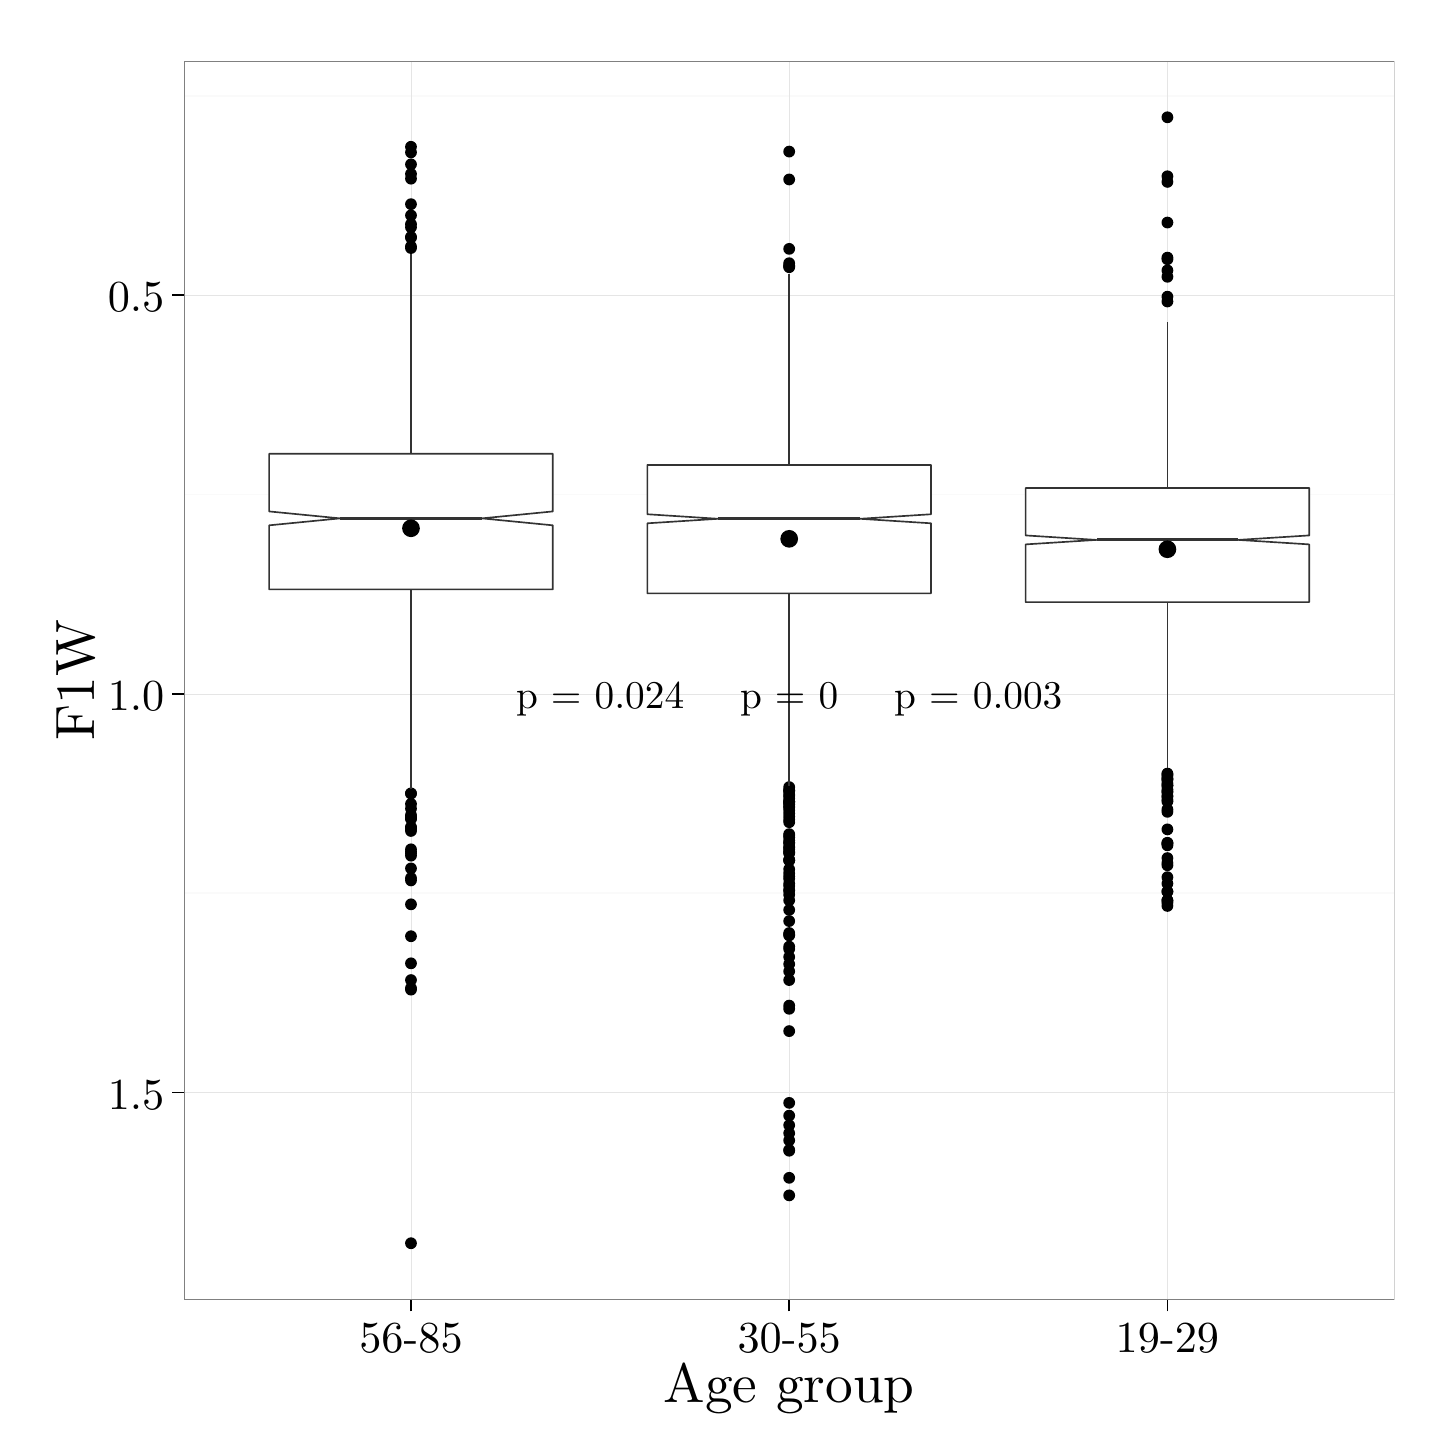
\begin{tikzpicture}[x=1pt,y=1pt]
\definecolor{fillColor}{RGB}{255,255,255}
\path[use as bounding box,fill=fillColor,fill opacity=0.00] (0,0) rectangle (505.89,505.89);
\begin{scope}
\path[clip] (  0.00,  0.00) rectangle (505.89,505.89);
\definecolor{drawColor}{RGB}{255,255,255}
\definecolor{fillColor}{RGB}{255,255,255}

\path[draw=drawColor,line width= 0.6pt,line join=round,line cap=round,fill=fillColor] (  0.00, -0.00) rectangle (505.89,505.89);
\end{scope}
\begin{scope}
\path[clip] ( 56.50, 46.31) rectangle (493.85,493.84);
\definecolor{fillColor}{RGB}{255,255,255}

\path[fill=fillColor] ( 56.50, 46.31) rectangle (493.85,493.84);
\definecolor{drawColor}{gray}{0.98}

\path[draw=drawColor,line width= 0.6pt,line join=round] ( 56.50,481.28) --
	(493.85,481.28);

\path[draw=drawColor,line width= 0.6pt,line join=round] ( 56.50,337.21) --
	(493.85,337.21);

\path[draw=drawColor,line width= 0.6pt,line join=round] ( 56.50,193.14) --
	(493.85,193.14);
\definecolor{drawColor}{gray}{0.90}

\path[draw=drawColor,line width= 0.2pt,line join=round] ( 56.50,409.25) --
	(493.85,409.25);

\path[draw=drawColor,line width= 0.2pt,line join=round] ( 56.50,265.18) --
	(493.85,265.18);

\path[draw=drawColor,line width= 0.2pt,line join=round] ( 56.50,121.11) --
	(493.85,121.11);

\path[draw=drawColor,line width= 0.2pt,line join=round] (138.51, 46.31) --
	(138.51,493.84);

\path[draw=drawColor,line width= 0.2pt,line join=round] (275.17, 46.31) --
	(275.17,493.84);

\path[draw=drawColor,line width= 0.2pt,line join=round] (411.84, 46.31) --
	(411.84,493.84);
\definecolor{fillColor}{RGB}{0,0,0}

\path[fill=fillColor] (138.51,220.23) circle (  2.13);

\path[fill=fillColor] (138.51,442.10) circle (  2.13);

\path[fill=fillColor] (138.51,456.50) circle (  2.13);

\path[fill=fillColor] (138.51,429.99) circle (  2.13);

\path[fill=fillColor] (138.51,434.89) circle (  2.13);

\path[fill=fillColor] (138.51,158.28) circle (  2.13);

\path[fill=fillColor] (138.51,215.62) circle (  2.13);

\path[fill=fillColor] (138.51,198.62) circle (  2.13);

\path[fill=fillColor] (138.51,208.99) circle (  2.13);

\path[fill=fillColor] (138.51,216.48) circle (  2.13);

\path[fill=fillColor] (138.51,217.06) circle (  2.13);

\path[fill=fillColor] (138.51,216.77) circle (  2.13);

\path[fill=fillColor] (138.51,223.69) circle (  2.13);

\path[fill=fillColor] (138.51,207.55) circle (  2.13);

\path[fill=fillColor] (138.51,220.52) circle (  2.13);

\path[fill=fillColor] (138.51,206.69) circle (  2.13);

\path[fill=fillColor] (138.51,219.94) circle (  2.13);

\path[fill=fillColor] (138.51,225.41) circle (  2.13);

\path[fill=fillColor] (138.51, 66.65) circle (  2.13);

\path[fill=fillColor] (138.51,197.75) circle (  2.13);

\path[fill=fillColor] (138.51,189.11) circle (  2.13);

\path[fill=fillColor] (138.51,202.08) circle (  2.13);

\path[fill=fillColor] (138.51,426.82) circle (  2.13);

\path[fill=fillColor] (138.51,208.13) circle (  2.13);

\path[fill=fillColor] (138.51,426.25) circle (  2.13);

\path[fill=fillColor] (138.51,221.38) circle (  2.13);

\path[fill=fillColor] (138.51,158.85) circle (  2.13);

\path[fill=fillColor] (138.51,229.16) circle (  2.13);

\path[fill=fillColor] (138.51,177.58) circle (  2.13);

\path[fill=fillColor] (138.51,161.74) circle (  2.13);

\path[fill=fillColor] (138.51,167.79) circle (  2.13);

\path[fill=fillColor] (138.51,229.16) circle (  2.13);

\path[fill=fillColor] (138.51,438.06) circle (  2.13);

\path[fill=fillColor] (138.51,462.84) circle (  2.13);

\path[fill=fillColor] (138.51,453.04) circle (  2.13);

\path[fill=fillColor] (138.51,451.32) circle (  2.13);

\path[fill=fillColor] (138.51,460.82) circle (  2.13);

\path[fill=fillColor] (138.51,430.28) circle (  2.13);

\path[fill=fillColor] (138.51,433.74) circle (  2.13);
\definecolor{drawColor}{gray}{0.20}

\path[draw=drawColor,line width= 0.6pt,line join=round] (138.51,351.91) -- (138.51,423.94);

\path[draw=drawColor,line width= 0.6pt,line join=round] (138.51,302.92) -- (138.51,230.89);
\definecolor{fillColor}{RGB}{255,255,255}

\path[draw=drawColor,line width= 0.6pt,line join=round,line cap=round,fill=fillColor] ( 87.25,351.91) --
	( 87.25,331.08) --
	(112.88,328.57) --
	( 87.25,326.06) --
	( 87.25,302.92) --
	(189.76,302.92) --
	(189.76,326.06) --
	(164.13,328.57) --
	(189.76,331.08) --
	(189.76,351.91) --
	( 87.25,351.91) --
	cycle;

\path[draw=drawColor,line width= 1.1pt,line join=round] (112.88,328.57) -- (164.13,328.57);
\definecolor{fillColor}{RGB}{0,0,0}

\path[fill=fillColor] (275.17,209.57) circle (  2.13);

\path[fill=fillColor] (275.17,226.28) circle (  2.13);

\path[fill=fillColor] (275.17,207.55) circle (  2.13);

\path[fill=fillColor] (275.17,200.35) circle (  2.13);

\path[fill=fillColor] (275.17,212.16) circle (  2.13);

\path[fill=fillColor] (275.17,227.43) circle (  2.13);

\path[fill=fillColor] (275.17,152.52) circle (  2.13);

\path[fill=fillColor] (275.17,231.47) circle (  2.13);

\path[fill=fillColor] (275.17,213.89) circle (  2.13);

\path[fill=fillColor] (275.17,218.79) circle (  2.13);

\path[fill=fillColor] (275.17,225.13) circle (  2.13);

\path[fill=fillColor] (275.17,201.79) circle (  2.13);

\path[fill=fillColor] (275.17,225.70) circle (  2.13);

\path[fill=fillColor] (275.17,226.28) circle (  2.13);

\path[fill=fillColor] (275.17,143.30) circle (  2.13);

\path[fill=fillColor] (275.17,214.47) circle (  2.13);

\path[fill=fillColor] (275.17,192.57) circle (  2.13);

\path[fill=fillColor] (275.17,223.11) circle (  2.13);

\path[fill=fillColor] (275.17,190.55) circle (  2.13);

\path[fill=fillColor] (275.17,221.96) circle (  2.13);

\path[fill=fillColor] (275.17,177.87) circle (  2.13);

\path[fill=fillColor] (275.17,195.74) circle (  2.13);

\path[fill=fillColor] (275.17, 83.94) circle (  2.13);

\path[fill=fillColor] (275.17,205.24) circle (  2.13);

\path[fill=fillColor] (275.17,224.26) circle (  2.13);

\path[fill=fillColor] (275.17,109.29) circle (  2.13);

\path[fill=fillColor] (275.17,100.36) circle (  2.13);

\path[fill=fillColor] (275.17,151.36) circle (  2.13);

\path[fill=fillColor] (275.17, 90.28) circle (  2.13);

\path[fill=fillColor] (275.17,228.87) circle (  2.13);

\path[fill=fillColor] (275.17,112.75) circle (  2.13);

\path[fill=fillColor] (275.17,194.01) circle (  2.13);

\path[fill=fillColor] (275.17,461.11) circle (  2.13);

\path[fill=fillColor] (275.17,196.60) circle (  2.13);

\path[fill=fillColor] (275.17,117.36) circle (  2.13);

\path[fill=fillColor] (275.17,100.07) circle (  2.13);

\path[fill=fillColor] (275.17,106.41) circle (  2.13);

\path[fill=fillColor] (275.17,211.30) circle (  2.13);

\path[fill=fillColor] (275.17,103.82) circle (  2.13);

\path[fill=fillColor] (275.17,419.33) circle (  2.13);

\path[fill=fillColor] (275.17,419.62) circle (  2.13);

\path[fill=fillColor] (275.17,167.50) circle (  2.13);

\path[fill=fillColor] (275.17,161.74) circle (  2.13);

\path[fill=fillColor] (275.17,425.96) circle (  2.13);

\path[fill=fillColor] (275.17,219.65) circle (  2.13);

\path[fill=fillColor] (275.17,199.19) circle (  2.13);

\path[fill=fillColor] (275.17,419.91) circle (  2.13);

\path[fill=fillColor] (275.17,164.91) circle (  2.13);

\path[fill=fillColor] (275.17,228.30) circle (  2.13);

\path[fill=fillColor] (275.17,178.16) circle (  2.13);

\path[fill=fillColor] (275.17,420.77) circle (  2.13);

\path[fill=fillColor] (275.17,170.09) circle (  2.13);

\path[fill=fillColor] (275.17,183.06) circle (  2.13);

\path[fill=fillColor] (275.17,178.74) circle (  2.13);

\path[fill=fillColor] (275.17,194.30) circle (  2.13);

\path[fill=fillColor] (275.17,209.86) circle (  2.13);

\path[fill=fillColor] (275.17,230.02) circle (  2.13);

\path[fill=fillColor] (275.17,208.99) circle (  2.13);

\path[fill=fillColor] (275.17,225.99) circle (  2.13);

\path[fill=fillColor] (275.17,211.30) circle (  2.13);

\path[fill=fillColor] (275.17,198.33) circle (  2.13);

\path[fill=fillColor] (275.17,187.09) circle (  2.13);

\path[fill=fillColor] (275.17,208.13) circle (  2.13);

\path[fill=fillColor] (275.17,220.80) circle (  2.13);

\path[fill=fillColor] (275.17,173.84) circle (  2.13);

\path[fill=fillColor] (275.17,172.97) circle (  2.13);

\path[fill=fillColor] (275.17,204.96) circle (  2.13);

\path[fill=fillColor] (275.17,207.84) circle (  2.13);

\path[fill=fillColor] (275.17,451.03) circle (  2.13);

\path[fill=fillColor] (275.17,230.31) circle (  2.13);

\path[fill=fillColor] (275.17,213.31) circle (  2.13);

\path[fill=fillColor] (275.17,224.26) circle (  2.13);

\path[fill=fillColor] (275.17,204.96) circle (  2.13);

\path[fill=fillColor] (275.17,230.31) circle (  2.13);

\path[draw=drawColor,line width= 0.6pt,line join=round] (275.17,347.87) -- (275.17,416.74);

\path[draw=drawColor,line width= 0.6pt,line join=round] (275.17,301.48) -- (275.17,232.04);
\definecolor{fillColor}{RGB}{255,255,255}

\path[draw=drawColor,line width= 0.6pt,line join=round,line cap=round,fill=fillColor] (223.92,347.87) --
	(223.92,330.06) --
	(249.55,328.42) --
	(223.92,326.79) --
	(223.92,301.48) --
	(326.43,301.48) --
	(326.43,326.79) --
	(300.80,328.42) --
	(326.43,330.06) --
	(326.43,347.87) --
	(223.92,347.87) --
	cycle;

\path[draw=drawColor,line width= 1.1pt,line join=round] (249.55,328.42) -- (300.80,328.42);
\definecolor{fillColor}{RGB}{0,0,0}

\path[fill=fillColor] (411.84,450.16) circle (  2.13);

\path[fill=fillColor] (411.84,204.09) circle (  2.13);

\path[fill=fillColor] (411.84,408.67) circle (  2.13);

\path[fill=fillColor] (411.84,230.60) circle (  2.13);

\path[fill=fillColor] (411.84,473.50) circle (  2.13);

\path[fill=fillColor] (411.84,193.72) circle (  2.13);

\path[fill=fillColor] (411.84,406.94) circle (  2.13);

\path[fill=fillColor] (411.84,415.87) circle (  2.13);

\path[fill=fillColor] (411.84,205.82) circle (  2.13);

\path[fill=fillColor] (411.84,228.01) circle (  2.13);

\path[fill=fillColor] (411.84,435.47) circle (  2.13);

\path[fill=fillColor] (411.84,189.69) circle (  2.13);

\path[fill=fillColor] (411.84,422.21) circle (  2.13);

\path[fill=fillColor] (411.84,216.19) circle (  2.13);

\path[fill=fillColor] (411.84,203.23) circle (  2.13);

\path[fill=fillColor] (411.84,452.18) circle (  2.13);

\path[fill=fillColor] (411.84,223.40) circle (  2.13);

\path[fill=fillColor] (411.84,190.55) circle (  2.13);

\path[fill=fillColor] (411.84,211.30) circle (  2.13);

\path[fill=fillColor] (411.84,232.04) circle (  2.13);

\path[fill=fillColor] (411.84,226.28) circle (  2.13);

\path[fill=fillColor] (411.84,228.30) circle (  2.13);

\path[fill=fillColor] (411.84,188.53) circle (  2.13);

\path[fill=fillColor] (411.84,235.50) circle (  2.13);

\path[fill=fillColor] (411.84,422.79) circle (  2.13);

\path[fill=fillColor] (411.84,210.43) circle (  2.13);

\path[fill=fillColor] (411.84,222.53) circle (  2.13);

\path[fill=fillColor] (411.84,190.55) circle (  2.13);

\path[fill=fillColor] (411.84,229.74) circle (  2.13);

\path[fill=fillColor] (411.84,232.91) circle (  2.13);

\path[fill=fillColor] (411.84,198.91) circle (  2.13);

\path[fill=fillColor] (411.84,226.86) circle (  2.13);

\path[fill=fillColor] (411.84,236.36) circle (  2.13);

\path[fill=fillColor] (411.84,211.01) circle (  2.13);

\path[fill=fillColor] (411.84,211.30) circle (  2.13);

\path[fill=fillColor] (411.84,196.60) circle (  2.13);

\path[fill=fillColor] (411.84,232.04) circle (  2.13);

\path[fill=fillColor] (411.84,236.08) circle (  2.13);

\path[fill=fillColor] (411.84,418.18) circle (  2.13);

\path[fill=fillColor] (411.84,234.35) circle (  2.13);

\path[fill=fillColor] (411.84,234.64) circle (  2.13);

\path[fill=fillColor] (411.84,234.06) circle (  2.13);

\path[fill=fillColor] (411.84,193.72) circle (  2.13);

\path[fill=fillColor] (411.84,229.74) circle (  2.13);

\path[draw=drawColor,line width= 0.6pt,line join=round] (411.84,339.52) -- (411.84,399.45);

\path[draw=drawColor,line width= 0.6pt,line join=round] (411.84,298.31) -- (411.84,238.38);
\definecolor{fillColor}{RGB}{255,255,255}

\path[draw=drawColor,line width= 0.6pt,line join=round,line cap=round,fill=fillColor] (360.59,339.52) --
	(360.59,322.41) --
	(386.22,320.79) --
	(360.59,319.17) --
	(360.59,298.31) --
	(463.09,298.31) --
	(463.09,319.17) --
	(437.47,320.79) --
	(463.09,322.41) --
	(463.09,339.52) --
	(360.59,339.52) --
	cycle;

\path[draw=drawColor,line width= 1.1pt,line join=round] (386.22,320.79) -- (437.47,320.79);
\definecolor{fillColor}{RGB}{0,0,0}

\path[fill=fillColor] (138.51,324.99) circle (  3.20);

\path[fill=fillColor] (275.17,321.18) circle (  3.20);

\path[fill=fillColor] (411.84,317.41) circle (  3.20);
\definecolor{drawColor}{RGB}{0,0,0}

\node[text=drawColor,anchor=base,inner sep=0pt, outer sep=0pt, scale=  1.42] at (206.84,259.83) {p = 0.024};

\node[text=drawColor,anchor=base,inner sep=0pt, outer sep=0pt, scale=  1.42] at (343.51,259.83) {p = 0.003};

\node[text=drawColor,anchor=base,inner sep=0pt, outer sep=0pt, scale=  1.42] at (275.17,259.83) {p = 0};
\definecolor{drawColor}{gray}{0.50}

\path[draw=drawColor,line width= 0.6pt,line join=round,line cap=round] ( 56.50, 46.31) rectangle (493.85,493.84);
\end{scope}
\begin{scope}
\path[clip] (  0.00,  0.00) rectangle (505.89,505.89);
\definecolor{drawColor}{RGB}{0,0,0}

\node[text=drawColor,anchor=base east,inner sep=0pt, outer sep=0pt, scale=  1.60] at ( 49.39,403.21) {0.5};

\node[text=drawColor,anchor=base east,inner sep=0pt, outer sep=0pt, scale=  1.60] at ( 49.39,259.14) {1.0};

\node[text=drawColor,anchor=base east,inner sep=0pt, outer sep=0pt, scale=  1.60] at ( 49.39,115.08) {1.5};
\end{scope}
\begin{scope}
\path[clip] (  0.00,  0.00) rectangle (505.89,505.89);
\definecolor{drawColor}{RGB}{0,0,0}

\path[draw=drawColor,line width= 0.6pt,line join=round] ( 52.24,409.25) --
	( 56.50,409.25);

\path[draw=drawColor,line width= 0.6pt,line join=round] ( 52.24,265.18) --
	( 56.50,265.18);

\path[draw=drawColor,line width= 0.6pt,line join=round] ( 52.24,121.11) --
	( 56.50,121.11);
\end{scope}
\begin{scope}
\path[clip] (  0.00,  0.00) rectangle (505.89,505.89);
\definecolor{drawColor}{RGB}{0,0,0}

\path[draw=drawColor,line width= 0.6pt,line join=round] (138.51, 42.04) --
	(138.51, 46.31);

\path[draw=drawColor,line width= 0.6pt,line join=round] (275.17, 42.04) --
	(275.17, 46.31);

\path[draw=drawColor,line width= 0.6pt,line join=round] (411.84, 42.04) --
	(411.84, 46.31);
\end{scope}
\begin{scope}
\path[clip] (  0.00,  0.00) rectangle (505.89,505.89);
\definecolor{drawColor}{RGB}{0,0,0}

\node[text=drawColor,anchor=base,inner sep=0pt, outer sep=0pt, scale=  1.60] at (138.51, 27.13) {56-85};

\node[text=drawColor,anchor=base,inner sep=0pt, outer sep=0pt, scale=  1.60] at (275.17, 27.13) {30-55};

\node[text=drawColor,anchor=base,inner sep=0pt, outer sep=0pt, scale=  1.60] at (411.84, 27.13) {19-29};
\end{scope}
\begin{scope}
\path[clip] (  0.00,  0.00) rectangle (505.89,505.89);
\definecolor{drawColor}{RGB}{0,0,0}

\node[text=drawColor,anchor=base,inner sep=0pt, outer sep=0pt, scale=  2.00] at (275.17,  9.03) {Age group};
\end{scope}
\begin{scope}
\path[clip] (  0.00,  0.00) rectangle (505.89,505.89);
\definecolor{drawColor}{RGB}{0,0,0}

\node[text=drawColor,rotate= 90.00,anchor=base,inner sep=0pt, outer sep=0pt, scale=  2.00] at ( 24.12,270.08) {F1W};
\end{scope}
\end{tikzpicture}
} 
	\caption{happ\textsc{y} (F1) by age}
	\label{fig.box.f1w.happy.tot}
\end{figure}

Most importantly, however, it is obvious from Figure \ref{fig.box.f1w.happy.tot} that the hypothesis that younger speakers are, on average, more Scouse cannot be confirmed with respect to the height of happ\textsc{y}.
Both mean and (to a lesser extent) median values decrease `graphically' (due to the inverted y-axis; in numeric terms they of course \emph{in}crease) from left to right.
Average F1 thus significantly increases from the old to the middle-aged group (t(1838.232) = 2.257, p = 0.024), and from the middle-aged to the young (t(3609.648) = 2.949, p = 0.003), meaning that happ\textsc{y} systematically becomes \emph{lower}, i.e. less Scouse, the younger the speaker.
Liverpudlians between the ages of 19 and 29 are therefore actually the \emph{least} Scouse in the sample, because they have lower realisations of happ\textsc{y} than their parents' generation, who in turn use lower variants than the oldest speakers.

How does this predictor interact with gender, then?
In Figure \ref{fig.scatter.f1w.happy.genderage}, we again (cf. Figure \ref{fig.scatter.f1w.happy.genderclass}) see gender of participant on the x-axis and estimated F1 on the y-axis, but it is now age of participant instead of social class which is coded by line type (solid for the oldest, dotted for the middle-aged, and dashed for the youngest speakers).
Just as in the corresponding graph for gender and social class, it is obvious that women seem to be behind the age differences described in the preceding paragraphs.
Only for female subjects are the lines clearly distinct from one another.
For male speakers, on the right-hand side, the regression lines of all age groups are either in, or at least very close to, the dark grey area which marks overlapping standard deviations.
This indicates that age groups are not significantly different from one another if only the male subjects are considered.
Table \ref{tab.happy.genderage.pvalues} shows that this is indeed the case: t-tests of all three pairings (comparing the old speakers to the middle-aged, the middle-aged to the young, and the young to the old) yield highly significant results for female, and non-significant ones for male subjects across the board.

\begin{table}[h!]
	\centering
	\caption{happ\textsc{y} (F1): t-tests of age by gender}
	\label{tab.happy.genderage.pvalues}
	\begin{tabular}{lcccccc}
		\hline
		test & \multicolumn{3}{c}{women} & \multicolumn{3}{c}{men}\\
		& t & df & p & t & df & p\\
		\hline
		old-middle & 4.062 & 1091.324 & < 0.001 & \ensuremath{-1.368} & 798.429 & 0.172\\
		middle-young & 5.062 & 1596.832 & < 0.001 & \ensuremath{-0.333} & 1999.537 & 0.739\\
		young-old & 8.689 & 888.424 & < 0.001 & \ensuremath{-1.624} & 768.511 & 0.105\\			 
		\hline			
	\end{tabular}
\end{table}

\begin{figure}[h!]
	\centering
	\begin{subfigure}{.49\textwidth}
		\centering
			\definecolor{shadecolor}{rgb}{0.969, 0.969, 0.969}
			\resizebox{\linewidth}{!}{% Created by tikzDevice version 0.8.1 on 2016-02-09 02:13:06
% !TEX encoding = UTF-8 Unicode
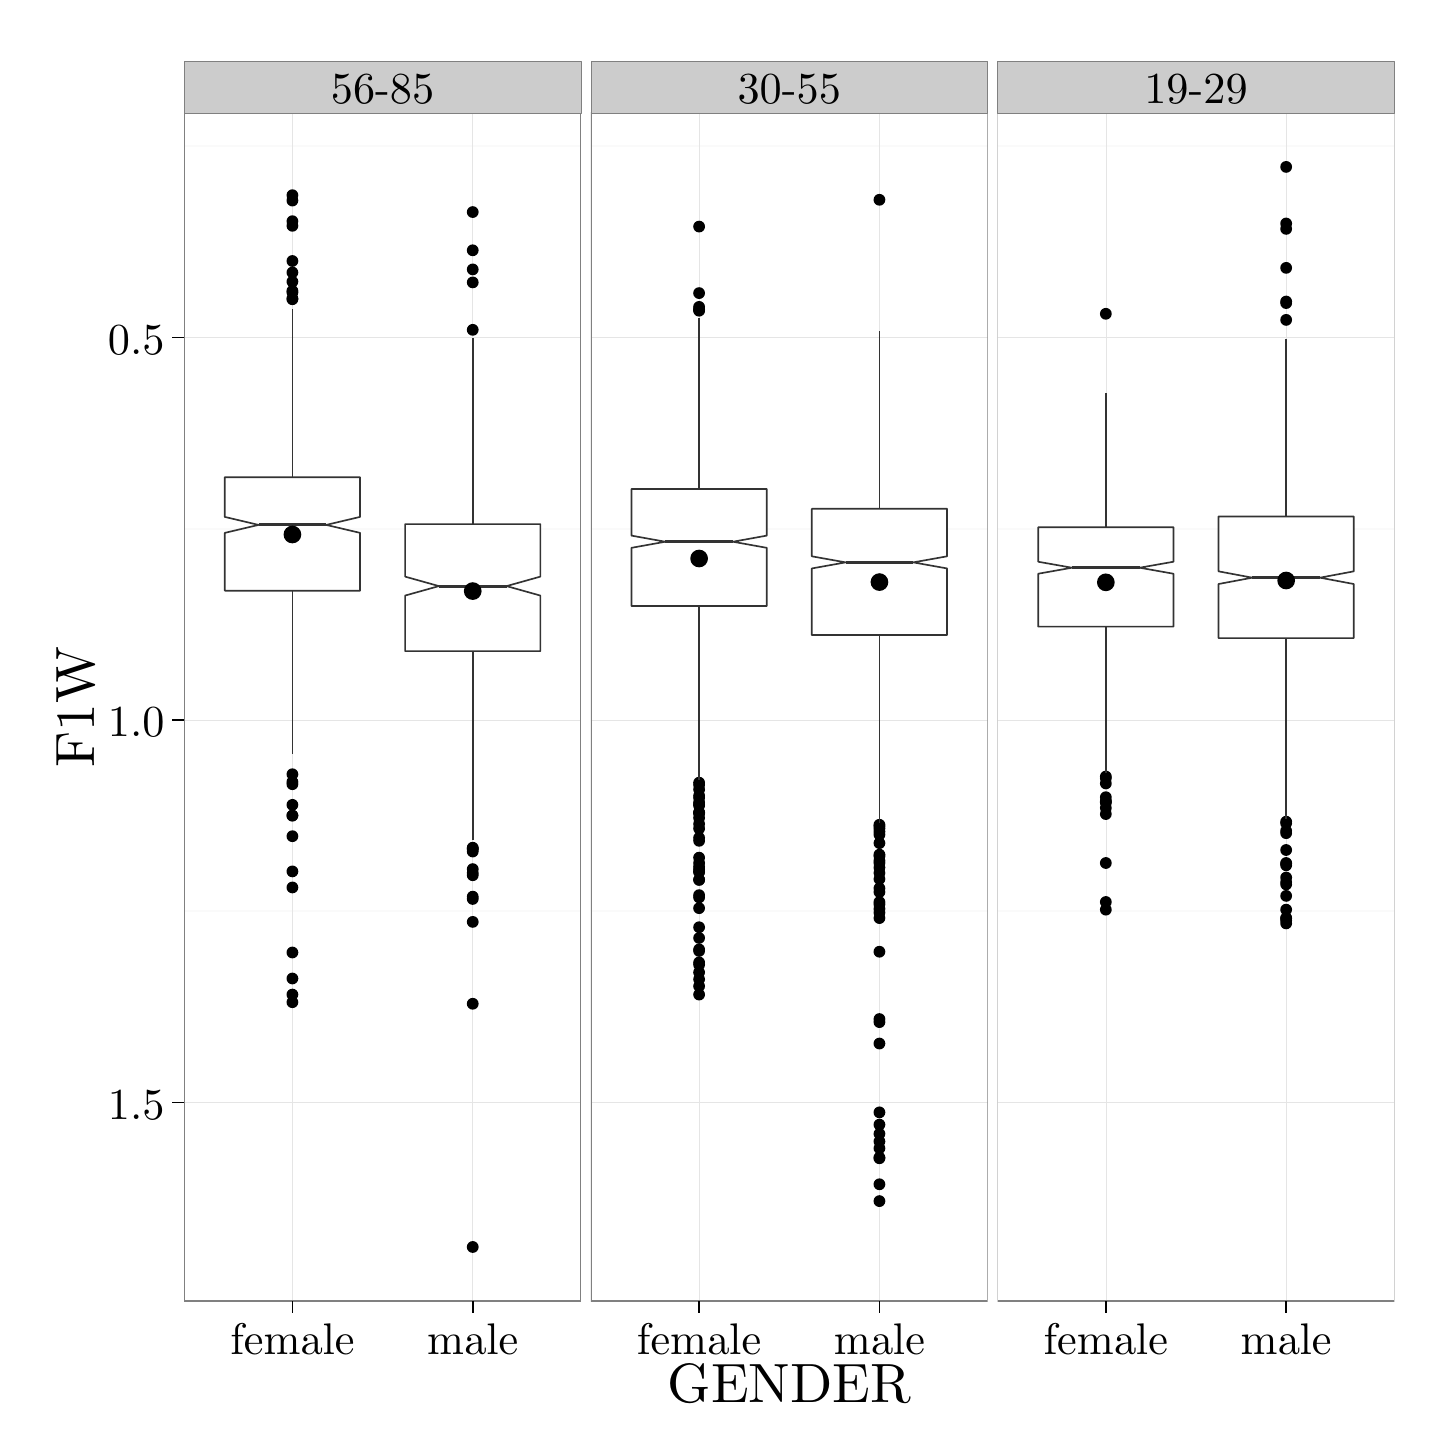
\begin{tikzpicture}[x=1pt,y=1pt]
\definecolor{fillColor}{RGB}{255,255,255}
\path[use as bounding box,fill=fillColor,fill opacity=0.00] (0,0) rectangle (505.89,505.89);
\begin{scope}
\path[clip] (  0.00,  0.00) rectangle (505.89,505.89);
\definecolor{drawColor}{RGB}{255,255,255}
\definecolor{fillColor}{RGB}{255,255,255}

\path[draw=drawColor,line width= 0.6pt,line join=round,line cap=round,fill=fillColor] (  0.00, -0.00) rectangle (505.89,505.89);
\end{scope}
\begin{scope}
\path[clip] ( 56.56, 45.77) rectangle (199.92,475.09);
\definecolor{fillColor}{RGB}{255,255,255}

\path[fill=fillColor] ( 56.56, 45.77) rectangle (199.92,475.09);
\definecolor{drawColor}{gray}{0.98}

\path[draw=drawColor,line width= 0.6pt,line join=round] ( 56.56,463.04) --
	(199.92,463.04);

\path[draw=drawColor,line width= 0.6pt,line join=round] ( 56.56,324.83) --
	(199.92,324.83);

\path[draw=drawColor,line width= 0.6pt,line join=round] ( 56.56,186.63) --
	(199.92,186.63);
\definecolor{drawColor}{gray}{0.90}

\path[draw=drawColor,line width= 0.2pt,line join=round] ( 56.56,393.93) --
	(199.92,393.93);

\path[draw=drawColor,line width= 0.2pt,line join=round] ( 56.56,255.73) --
	(199.92,255.73);

\path[draw=drawColor,line width= 0.2pt,line join=round] ( 56.56,117.53) --
	(199.92,117.53);

\path[draw=drawColor,line width= 0.2pt,line join=round] ( 95.66, 45.77) --
	( 95.66,475.09);

\path[draw=drawColor,line width= 0.2pt,line join=round] (160.82, 45.77) --
	(160.82,475.09);
\definecolor{fillColor}{RGB}{0,0,0}

\path[fill=fillColor] ( 95.66,233.34) circle (  2.13);

\path[fill=fillColor] ( 95.66,195.20) circle (  2.13);

\path[fill=fillColor] ( 95.66,232.51) circle (  2.13);

\path[fill=fillColor] ( 95.66,410.79) circle (  2.13);

\path[fill=fillColor] ( 95.66,201.00) circle (  2.13);

\path[fill=fillColor] ( 95.66,407.75) circle (  2.13);

\path[fill=fillColor] ( 95.66,225.05) circle (  2.13);

\path[fill=fillColor] ( 95.66,410.24) circle (  2.13);

\path[fill=fillColor] ( 95.66,213.72) circle (  2.13);

\path[fill=fillColor] ( 95.66,153.74) circle (  2.13);

\path[fill=fillColor] ( 95.66,221.18) circle (  2.13);

\path[fill=fillColor] ( 95.66,171.70) circle (  2.13);

\path[fill=fillColor] ( 95.66,156.50) circle (  2.13);

\path[fill=fillColor] ( 95.66,162.31) circle (  2.13);

\path[fill=fillColor] ( 95.66,221.18) circle (  2.13);

\path[fill=fillColor] ( 95.66,421.57) circle (  2.13);

\path[fill=fillColor] ( 95.66,445.35) circle (  2.13);

\path[fill=fillColor] ( 95.66,435.95) circle (  2.13);

\path[fill=fillColor] ( 95.66,434.29) circle (  2.13);

\path[fill=fillColor] ( 95.66,443.41) circle (  2.13);

\path[fill=fillColor] ( 95.66,414.11) circle (  2.13);

\path[fill=fillColor] ( 95.66,417.43) circle (  2.13);

\path[fill=fillColor] ( 95.66,236.11) circle (  2.13);

\path[fill=fillColor] ( 95.66,408.03) circle (  2.13);
\definecolor{drawColor}{gray}{0.20}

\path[draw=drawColor,line width= 0.6pt,line join=round] ( 95.66,343.42) -- ( 95.66,404.16);

\path[draw=drawColor,line width= 0.6pt,line join=round] ( 95.66,302.44) -- ( 95.66,243.29);
\definecolor{fillColor}{RGB}{255,255,255}

\path[draw=drawColor,line width= 0.6pt,line join=round,line cap=round,fill=fillColor] ( 71.23,343.42) --
	( 71.23,329.10) --
	( 83.44,326.21) --
	( 71.23,323.33) --
	( 71.23,302.44) --
	(120.10,302.44) --
	(120.10,323.33) --
	(107.88,326.21) --
	(120.10,329.10) --
	(120.10,343.42) --
	( 71.23,343.42) --
	cycle;

\path[draw=drawColor,line width= 1.1pt,line join=round] ( 83.44,326.21) -- (107.88,326.21);
\definecolor{fillColor}{RGB}{0,0,0}

\path[fill=fillColor] (160.82,425.44) circle (  2.13);

\path[fill=fillColor] (160.82,439.26) circle (  2.13);

\path[fill=fillColor] (160.82,413.84) circle (  2.13);

\path[fill=fillColor] (160.82,418.53) circle (  2.13);

\path[fill=fillColor] (160.82,153.18) circle (  2.13);

\path[fill=fillColor] (160.82,396.70) circle (  2.13);

\path[fill=fillColor] (160.82,208.19) circle (  2.13);

\path[fill=fillColor] (160.82,191.88) circle (  2.13);

\path[fill=fillColor] (160.82,201.83) circle (  2.13);

\path[fill=fillColor] (160.82,209.02) circle (  2.13);

\path[fill=fillColor] (160.82,209.57) circle (  2.13);

\path[fill=fillColor] (160.82,209.29) circle (  2.13);

\path[fill=fillColor] (160.82,200.45) circle (  2.13);

\path[fill=fillColor] (160.82,199.62) circle (  2.13);

\path[fill=fillColor] (160.82, 65.29) circle (  2.13);

\path[fill=fillColor] (160.82,191.05) circle (  2.13);

\path[fill=fillColor] (160.82,182.76) circle (  2.13);

\path[draw=drawColor,line width= 0.6pt,line join=round] (160.82,326.49) -- (160.82,393.66);

\path[draw=drawColor,line width= 0.6pt,line join=round] (160.82,280.61) -- (160.82,212.33);
\definecolor{fillColor}{RGB}{255,255,255}

\path[draw=drawColor,line width= 0.6pt,line join=round,line cap=round,fill=fillColor] (136.39,326.49) --
	(136.39,307.52) --
	(148.60,304.10) --
	(136.39,300.68) --
	(136.39,280.61) --
	(185.25,280.61) --
	(185.25,300.68) --
	(173.04,304.10) --
	(185.25,307.52) --
	(185.25,326.49) --
	(136.39,326.49) --
	cycle;

\path[draw=drawColor,line width= 1.1pt,line join=round] (148.60,304.10) -- (173.04,304.10);
\definecolor{fillColor}{RGB}{0,0,0}

\path[fill=fillColor] ( 95.66,322.74) circle (  3.20);

\path[fill=fillColor] (160.82,302.30) circle (  3.20);
\definecolor{drawColor}{gray}{0.50}

\path[draw=drawColor,line width= 0.6pt,line join=round,line cap=round] ( 56.56, 45.77) rectangle (199.92,475.09);
\end{scope}
\begin{scope}
\path[clip] (203.53, 45.77) rectangle (346.88,475.09);
\definecolor{fillColor}{RGB}{255,255,255}

\path[fill=fillColor] (203.53, 45.77) rectangle (346.88,475.09);
\definecolor{drawColor}{gray}{0.98}

\path[draw=drawColor,line width= 0.6pt,line join=round] (203.53,463.04) --
	(346.88,463.04);

\path[draw=drawColor,line width= 0.6pt,line join=round] (203.53,324.83) --
	(346.88,324.83);

\path[draw=drawColor,line width= 0.6pt,line join=round] (203.53,186.63) --
	(346.88,186.63);
\definecolor{drawColor}{gray}{0.90}

\path[draw=drawColor,line width= 0.2pt,line join=round] (203.53,393.93) --
	(346.88,393.93);

\path[draw=drawColor,line width= 0.2pt,line join=round] (203.53,255.73) --
	(346.88,255.73);

\path[draw=drawColor,line width= 0.2pt,line join=round] (203.53,117.53) --
	(346.88,117.53);

\path[draw=drawColor,line width= 0.2pt,line join=round] (242.62, 45.77) --
	(242.62,475.09);

\path[draw=drawColor,line width= 0.2pt,line join=round] (307.78, 45.77) --
	(307.78,475.09);
\definecolor{fillColor}{RGB}{0,0,0}

\path[fill=fillColor] (242.62,403.61) circle (  2.13);

\path[fill=fillColor] (242.62,403.88) circle (  2.13);

\path[fill=fillColor] (242.62,162.03) circle (  2.13);

\path[fill=fillColor] (242.62,156.50) circle (  2.13);

\path[fill=fillColor] (242.62,409.97) circle (  2.13);

\path[fill=fillColor] (242.62,212.06) circle (  2.13);

\path[fill=fillColor] (242.62,192.43) circle (  2.13);

\path[fill=fillColor] (242.62,404.16) circle (  2.13);

\path[fill=fillColor] (242.62,159.54) circle (  2.13);

\path[fill=fillColor] (242.62,220.35) circle (  2.13);

\path[fill=fillColor] (242.62,172.26) circle (  2.13);

\path[fill=fillColor] (242.62,404.99) circle (  2.13);

\path[fill=fillColor] (242.62,164.52) circle (  2.13);

\path[fill=fillColor] (242.62,232.24) circle (  2.13);

\path[fill=fillColor] (242.62,225.88) circle (  2.13);

\path[fill=fillColor] (242.62,176.95) circle (  2.13);

\path[fill=fillColor] (242.62,172.81) circle (  2.13);

\path[fill=fillColor] (242.62,187.73) circle (  2.13);

\path[fill=fillColor] (242.62,202.66) circle (  2.13);

\path[fill=fillColor] (242.62,224.77) circle (  2.13);

\path[fill=fillColor] (242.62,222.01) circle (  2.13);

\path[fill=fillColor] (242.62,201.83) circle (  2.13);

\path[fill=fillColor] (242.62,218.14) circle (  2.13);

\path[fill=fillColor] (242.62,204.04) circle (  2.13);

\path[fill=fillColor] (242.62,191.60) circle (  2.13);

\path[fill=fillColor] (242.62,180.82) circle (  2.13);

\path[fill=fillColor] (242.62,201.00) circle (  2.13);

\path[fill=fillColor] (242.62,213.16) circle (  2.13);

\path[fill=fillColor] (242.62,168.11) circle (  2.13);

\path[fill=fillColor] (242.62,167.28) circle (  2.13);

\path[fill=fillColor] (242.62,197.96) circle (  2.13);

\path[fill=fillColor] (242.62,228.37) circle (  2.13);

\path[fill=fillColor] (242.62,200.73) circle (  2.13);

\path[fill=fillColor] (242.62,434.01) circle (  2.13);

\path[fill=fillColor] (242.62,222.29) circle (  2.13);

\path[fill=fillColor] (242.62,205.98) circle (  2.13);

\path[fill=fillColor] (242.62,216.48) circle (  2.13);

\path[fill=fillColor] (242.62,230.58) circle (  2.13);

\path[fill=fillColor] (242.62,225.33) circle (  2.13);

\path[fill=fillColor] (242.62,227.54) circle (  2.13);

\path[fill=fillColor] (242.62,197.96) circle (  2.13);

\path[fill=fillColor] (242.62,222.29) circle (  2.13);

\path[fill=fillColor] (242.62,233.07) circle (  2.13);
\definecolor{drawColor}{gray}{0.20}

\path[draw=drawColor,line width= 0.6pt,line join=round] (242.62,339.21) -- (242.62,401.12);

\path[draw=drawColor,line width= 0.6pt,line join=round] (242.62,296.92) -- (242.62,233.89);
\definecolor{fillColor}{RGB}{255,255,255}

\path[draw=drawColor,line width= 0.6pt,line join=round,line cap=round,fill=fillColor] (218.19,339.21) --
	(218.19,322.34) --
	(230.41,320.13) --
	(218.19,317.93) --
	(218.19,296.92) --
	(267.06,296.92) --
	(267.06,317.93) --
	(254.84,320.13) --
	(267.06,322.34) --
	(267.06,339.21) --
	(218.19,339.21) --
	cycle;

\path[draw=drawColor,line width= 1.1pt,line join=round] (230.41,320.13) -- (254.84,320.13);
\definecolor{fillColor}{RGB}{0,0,0}

\path[fill=fillColor] (307.78,202.38) circle (  2.13);

\path[fill=fillColor] (307.78,200.45) circle (  2.13);

\path[fill=fillColor] (307.78,193.54) circle (  2.13);

\path[fill=fillColor] (307.78,204.87) circle (  2.13);

\path[fill=fillColor] (307.78,147.66) circle (  2.13);

\path[fill=fillColor] (307.78,206.53) circle (  2.13);

\path[fill=fillColor] (307.78,211.23) circle (  2.13);

\path[fill=fillColor] (307.78,217.31) circle (  2.13);

\path[fill=fillColor] (307.78,194.92) circle (  2.13);

\path[fill=fillColor] (307.78,217.86) circle (  2.13);

\path[fill=fillColor] (307.78,138.81) circle (  2.13);

\path[fill=fillColor] (307.78,207.08) circle (  2.13);

\path[fill=fillColor] (307.78,186.08) circle (  2.13);

\path[fill=fillColor] (307.78,215.38) circle (  2.13);

\path[fill=fillColor] (307.78,184.14) circle (  2.13);

\path[fill=fillColor] (307.78,214.27) circle (  2.13);

\path[fill=fillColor] (307.78,171.98) circle (  2.13);

\path[fill=fillColor] (307.78,189.12) circle (  2.13);

\path[fill=fillColor] (307.78, 81.87) circle (  2.13);

\path[fill=fillColor] (307.78,198.24) circle (  2.13);

\path[fill=fillColor] (307.78,216.48) circle (  2.13);

\path[fill=fillColor] (307.78,106.19) circle (  2.13);

\path[fill=fillColor] (307.78, 97.63) circle (  2.13);

\path[fill=fillColor] (307.78,146.55) circle (  2.13);

\path[fill=fillColor] (307.78, 87.95) circle (  2.13);

\path[fill=fillColor] (307.78,109.51) circle (  2.13);

\path[fill=fillColor] (307.78,187.46) circle (  2.13);

\path[fill=fillColor] (307.78,443.69) circle (  2.13);

\path[fill=fillColor] (307.78,189.95) circle (  2.13);

\path[fill=fillColor] (307.78,113.93) circle (  2.13);

\path[fill=fillColor] (307.78, 97.35) circle (  2.13);

\path[fill=fillColor] (307.78,103.43) circle (  2.13);

\path[fill=fillColor] (307.78,204.04) circle (  2.13);

\path[fill=fillColor] (307.78,100.94) circle (  2.13);

\path[draw=drawColor,line width= 0.6pt,line join=round] (307.78,332.02) -- (307.78,396.42);

\path[draw=drawColor,line width= 0.6pt,line join=round] (307.78,286.41) -- (307.78,218.42);
\definecolor{fillColor}{RGB}{255,255,255}

\path[draw=drawColor,line width= 0.6pt,line join=round,line cap=round,fill=fillColor] (283.35,332.02) --
	(283.35,314.86) --
	(295.57,312.67) --
	(283.35,310.48) --
	(283.35,286.41) --
	(332.22,286.41) --
	(332.22,310.48) --
	(320.00,312.67) --
	(332.22,314.86) --
	(332.22,332.02) --
	(283.35,332.02) --
	cycle;

\path[draw=drawColor,line width= 1.1pt,line join=round] (295.57,312.67) -- (320.00,312.67);
\definecolor{fillColor}{RGB}{0,0,0}

\path[fill=fillColor] (242.62,314.07) circle (  3.20);

\path[fill=fillColor] (307.78,305.55) circle (  3.20);
\definecolor{drawColor}{gray}{0.50}

\path[draw=drawColor,line width= 0.6pt,line join=round,line cap=round] (203.53, 45.77) rectangle (346.88,475.09);
\end{scope}
\begin{scope}
\path[clip] (350.49, 45.77) rectangle (493.85,475.09);
\definecolor{fillColor}{RGB}{255,255,255}

\path[fill=fillColor] (350.49, 45.77) rectangle (493.85,475.09);
\definecolor{drawColor}{gray}{0.98}

\path[draw=drawColor,line width= 0.6pt,line join=round] (350.49,463.04) --
	(493.85,463.04);

\path[draw=drawColor,line width= 0.6pt,line join=round] (350.49,324.83) --
	(493.85,324.83);

\path[draw=drawColor,line width= 0.6pt,line join=round] (350.49,186.63) --
	(493.85,186.63);
\definecolor{drawColor}{gray}{0.90}

\path[draw=drawColor,line width= 0.2pt,line join=round] (350.49,393.93) --
	(493.85,393.93);

\path[draw=drawColor,line width= 0.2pt,line join=round] (350.49,255.73) --
	(493.85,255.73);

\path[draw=drawColor,line width= 0.2pt,line join=round] (350.49,117.53) --
	(493.85,117.53);

\path[draw=drawColor,line width= 0.2pt,line join=round] (389.59, 45.77) --
	(389.59,475.09);

\path[draw=drawColor,line width= 0.2pt,line join=round] (454.75, 45.77) --
	(454.75,475.09);
\definecolor{fillColor}{RGB}{0,0,0}

\path[fill=fillColor] (389.59,204.04) circle (  2.13);

\path[fill=fillColor] (389.59,189.95) circle (  2.13);

\path[fill=fillColor] (389.59,223.94) circle (  2.13);

\path[fill=fillColor] (389.59,227.81) circle (  2.13);

\path[fill=fillColor] (389.59,402.50) circle (  2.13);

\path[fill=fillColor] (389.59,226.16) circle (  2.13);

\path[fill=fillColor] (389.59,226.43) circle (  2.13);

\path[fill=fillColor] (389.59,235.28) circle (  2.13);

\path[fill=fillColor] (389.59,234.72) circle (  2.13);

\path[fill=fillColor] (389.59,232.79) circle (  2.13);

\path[fill=fillColor] (389.59,225.88) circle (  2.13);

\path[fill=fillColor] (389.59,187.18) circle (  2.13);

\path[fill=fillColor] (389.59,221.73) circle (  2.13);
\definecolor{drawColor}{gray}{0.20}

\path[draw=drawColor,line width= 0.6pt,line join=round] (389.59,325.39) -- (389.59,374.03);

\path[draw=drawColor,line width= 0.6pt,line join=round] (389.59,289.45) -- (389.59,236.66);
\definecolor{fillColor}{RGB}{255,255,255}

\path[draw=drawColor,line width= 0.6pt,line join=round,line cap=round,fill=fillColor] (365.15,325.39) --
	(365.15,312.90) --
	(377.37,310.74) --
	(365.15,308.57) --
	(365.15,289.45) --
	(414.02,289.45) --
	(414.02,308.57) --
	(401.81,310.74) --
	(414.02,312.90) --
	(414.02,325.39) --
	(365.15,325.39) --
	cycle;

\path[draw=drawColor,line width= 1.1pt,line join=round] (377.37,310.74) -- (401.81,310.74);
\definecolor{fillColor}{RGB}{0,0,0}

\path[fill=fillColor] (454.75,433.18) circle (  2.13);

\path[fill=fillColor] (454.75,197.13) circle (  2.13);

\path[fill=fillColor] (454.75,455.57) circle (  2.13);

\path[fill=fillColor] (454.75,187.18) circle (  2.13);

\path[fill=fillColor] (454.75,400.29) circle (  2.13);

\path[fill=fillColor] (454.75,198.79) circle (  2.13);

\path[fill=fillColor] (454.75,419.09) circle (  2.13);

\path[fill=fillColor] (454.75,183.31) circle (  2.13);

\path[fill=fillColor] (454.75,406.37) circle (  2.13);

\path[fill=fillColor] (454.75,208.74) circle (  2.13);

\path[fill=fillColor] (454.75,196.30) circle (  2.13);

\path[fill=fillColor] (454.75,435.12) circle (  2.13);

\path[fill=fillColor] (454.75,215.65) circle (  2.13);

\path[fill=fillColor] (454.75,184.14) circle (  2.13);

\path[fill=fillColor] (454.75,204.04) circle (  2.13);

\path[fill=fillColor] (454.75,218.42) circle (  2.13);

\path[fill=fillColor] (454.75,182.21) circle (  2.13);

\path[fill=fillColor] (454.75,406.93) circle (  2.13);

\path[fill=fillColor] (454.75,203.21) circle (  2.13);

\path[fill=fillColor] (454.75,214.82) circle (  2.13);

\path[fill=fillColor] (454.75,184.14) circle (  2.13);

\path[fill=fillColor] (454.75,192.16) circle (  2.13);

\path[fill=fillColor] (454.75,218.97) circle (  2.13);

\path[fill=fillColor] (454.75,203.77) circle (  2.13);

\path[draw=drawColor,line width= 0.6pt,line join=round] (454.75,329.25) -- (454.75,393.38);

\path[draw=drawColor,line width= 0.6pt,line join=round] (454.75,285.31) -- (454.75,220.07);
\definecolor{fillColor}{RGB}{255,255,255}

\path[draw=drawColor,line width= 0.6pt,line join=round,line cap=round,fill=fillColor] (430.31,329.25) --
	(430.31,309.43) --
	(442.53,307.14) --
	(430.31,304.85) --
	(430.31,285.31) --
	(479.18,285.31) --
	(479.18,304.85) --
	(466.97,307.14) --
	(479.18,309.43) --
	(479.18,329.25) --
	(430.31,329.25) --
	cycle;

\path[draw=drawColor,line width= 1.1pt,line join=round] (442.53,307.14) -- (466.97,307.14);
\definecolor{fillColor}{RGB}{0,0,0}

\path[fill=fillColor] (389.59,305.46) circle (  3.20);

\path[fill=fillColor] (454.75,306.12) circle (  3.20);
\definecolor{drawColor}{gray}{0.50}

\path[draw=drawColor,line width= 0.6pt,line join=round,line cap=round] (350.49, 45.77) rectangle (493.85,475.09);
\end{scope}
\begin{scope}
\path[clip] (  0.00,  0.00) rectangle (505.89,505.89);
\definecolor{drawColor}{gray}{0.50}
\definecolor{fillColor}{gray}{0.80}

\path[draw=drawColor,line width= 0.2pt,line join=round,line cap=round,fill=fillColor] ( 56.56,475.09) rectangle (199.92,493.85);
\definecolor{drawColor}{RGB}{0,0,0}

\node[text=drawColor,anchor=base,inner sep=0pt, outer sep=0pt, scale=  1.60] at (128.24,478.43) {56-85};
\end{scope}
\begin{scope}
\path[clip] (  0.00,  0.00) rectangle (505.89,505.89);
\definecolor{drawColor}{gray}{0.50}
\definecolor{fillColor}{gray}{0.80}

\path[draw=drawColor,line width= 0.2pt,line join=round,line cap=round,fill=fillColor] (203.53,475.09) rectangle (346.88,493.85);
\definecolor{drawColor}{RGB}{0,0,0}

\node[text=drawColor,anchor=base,inner sep=0pt, outer sep=0pt, scale=  1.60] at (275.20,478.43) {30-55};
\end{scope}
\begin{scope}
\path[clip] (  0.00,  0.00) rectangle (505.89,505.89);
\definecolor{drawColor}{gray}{0.50}
\definecolor{fillColor}{gray}{0.80}

\path[draw=drawColor,line width= 0.2pt,line join=round,line cap=round,fill=fillColor] (350.49,475.09) rectangle (493.85,493.85);
\definecolor{drawColor}{RGB}{0,0,0}

\node[text=drawColor,anchor=base,inner sep=0pt, outer sep=0pt, scale=  1.60] at (422.17,478.43) {19-29};
\end{scope}
\begin{scope}
\path[clip] (  0.00,  0.00) rectangle (505.89,505.89);
\definecolor{drawColor}{RGB}{0,0,0}

\node[text=drawColor,anchor=base east,inner sep=0pt, outer sep=0pt, scale=  1.60] at ( 49.45,387.90) {0.5};

\node[text=drawColor,anchor=base east,inner sep=0pt, outer sep=0pt, scale=  1.60] at ( 49.45,249.70) {1.0};

\node[text=drawColor,anchor=base east,inner sep=0pt, outer sep=0pt, scale=  1.60] at ( 49.45,111.49) {1.5};
\end{scope}
\begin{scope}
\path[clip] (  0.00,  0.00) rectangle (505.89,505.89);
\definecolor{drawColor}{RGB}{0,0,0}

\path[draw=drawColor,line width= 0.6pt,line join=round] ( 52.30,393.93) --
	( 56.56,393.93);

\path[draw=drawColor,line width= 0.6pt,line join=round] ( 52.30,255.73) --
	( 56.56,255.73);

\path[draw=drawColor,line width= 0.6pt,line join=round] ( 52.30,117.53) --
	( 56.56,117.53);
\end{scope}
\begin{scope}
\path[clip] (  0.00,  0.00) rectangle (505.89,505.89);
\definecolor{drawColor}{RGB}{0,0,0}

\path[draw=drawColor,line width= 0.6pt,line join=round] ( 95.66, 41.50) --
	( 95.66, 45.77);

\path[draw=drawColor,line width= 0.6pt,line join=round] (160.82, 41.50) --
	(160.82, 45.77);
\end{scope}
\begin{scope}
\path[clip] (  0.00,  0.00) rectangle (505.89,505.89);
\definecolor{drawColor}{RGB}{0,0,0}

\node[text=drawColor,anchor=base,inner sep=0pt, outer sep=0pt, scale=  1.60] at ( 95.66, 26.59) {female};

\node[text=drawColor,anchor=base,inner sep=0pt, outer sep=0pt, scale=  1.60] at (160.82, 26.59) {male};
\end{scope}
\begin{scope}
\path[clip] (  0.00,  0.00) rectangle (505.89,505.89);
\definecolor{drawColor}{RGB}{0,0,0}

\path[draw=drawColor,line width= 0.6pt,line join=round] (242.62, 41.50) --
	(242.62, 45.77);

\path[draw=drawColor,line width= 0.6pt,line join=round] (307.78, 41.50) --
	(307.78, 45.77);
\end{scope}
\begin{scope}
\path[clip] (  0.00,  0.00) rectangle (505.89,505.89);
\definecolor{drawColor}{RGB}{0,0,0}

\node[text=drawColor,anchor=base,inner sep=0pt, outer sep=0pt, scale=  1.60] at (242.62, 26.59) {female};

\node[text=drawColor,anchor=base,inner sep=0pt, outer sep=0pt, scale=  1.60] at (307.78, 26.59) {male};
\end{scope}
\begin{scope}
\path[clip] (  0.00,  0.00) rectangle (505.89,505.89);
\definecolor{drawColor}{RGB}{0,0,0}

\path[draw=drawColor,line width= 0.6pt,line join=round] (389.59, 41.50) --
	(389.59, 45.77);

\path[draw=drawColor,line width= 0.6pt,line join=round] (454.75, 41.50) --
	(454.75, 45.77);
\end{scope}
\begin{scope}
\path[clip] (  0.00,  0.00) rectangle (505.89,505.89);
\definecolor{drawColor}{RGB}{0,0,0}

\node[text=drawColor,anchor=base,inner sep=0pt, outer sep=0pt, scale=  1.60] at (389.59, 26.59) {female};

\node[text=drawColor,anchor=base,inner sep=0pt, outer sep=0pt, scale=  1.60] at (454.75, 26.59) {male};
\end{scope}
\begin{scope}
\path[clip] (  0.00,  0.00) rectangle (505.89,505.89);
\definecolor{drawColor}{RGB}{0,0,0}

\node[text=drawColor,anchor=base,inner sep=0pt, outer sep=0pt, scale=  2.00] at (275.20,  9.03) {GENDER};
\end{scope}
\begin{scope}
\path[clip] (  0.00,  0.00) rectangle (505.89,505.89);
\definecolor{drawColor}{RGB}{0,0,0}

\node[text=drawColor,rotate= 90.00,anchor=base,inner sep=0pt, outer sep=0pt, scale=  2.00] at ( 24.12,260.43) {F1W};
\end{scope}
\end{tikzpicture}
} 
		\caption{box plot}
		\label{fig.box.f1w.happy.genderage}
	\end{subfigure}
	\begin{subfigure}{.49\textwidth}
		\centering
			\definecolor{shadecolor}{rgb}{0.969, 0.969, 0.969}
			\resizebox{\linewidth}{!}{% Created by tikzDevice version 0.8.1 on 2016-02-09 02:13:06
% !TEX encoding = UTF-8 Unicode
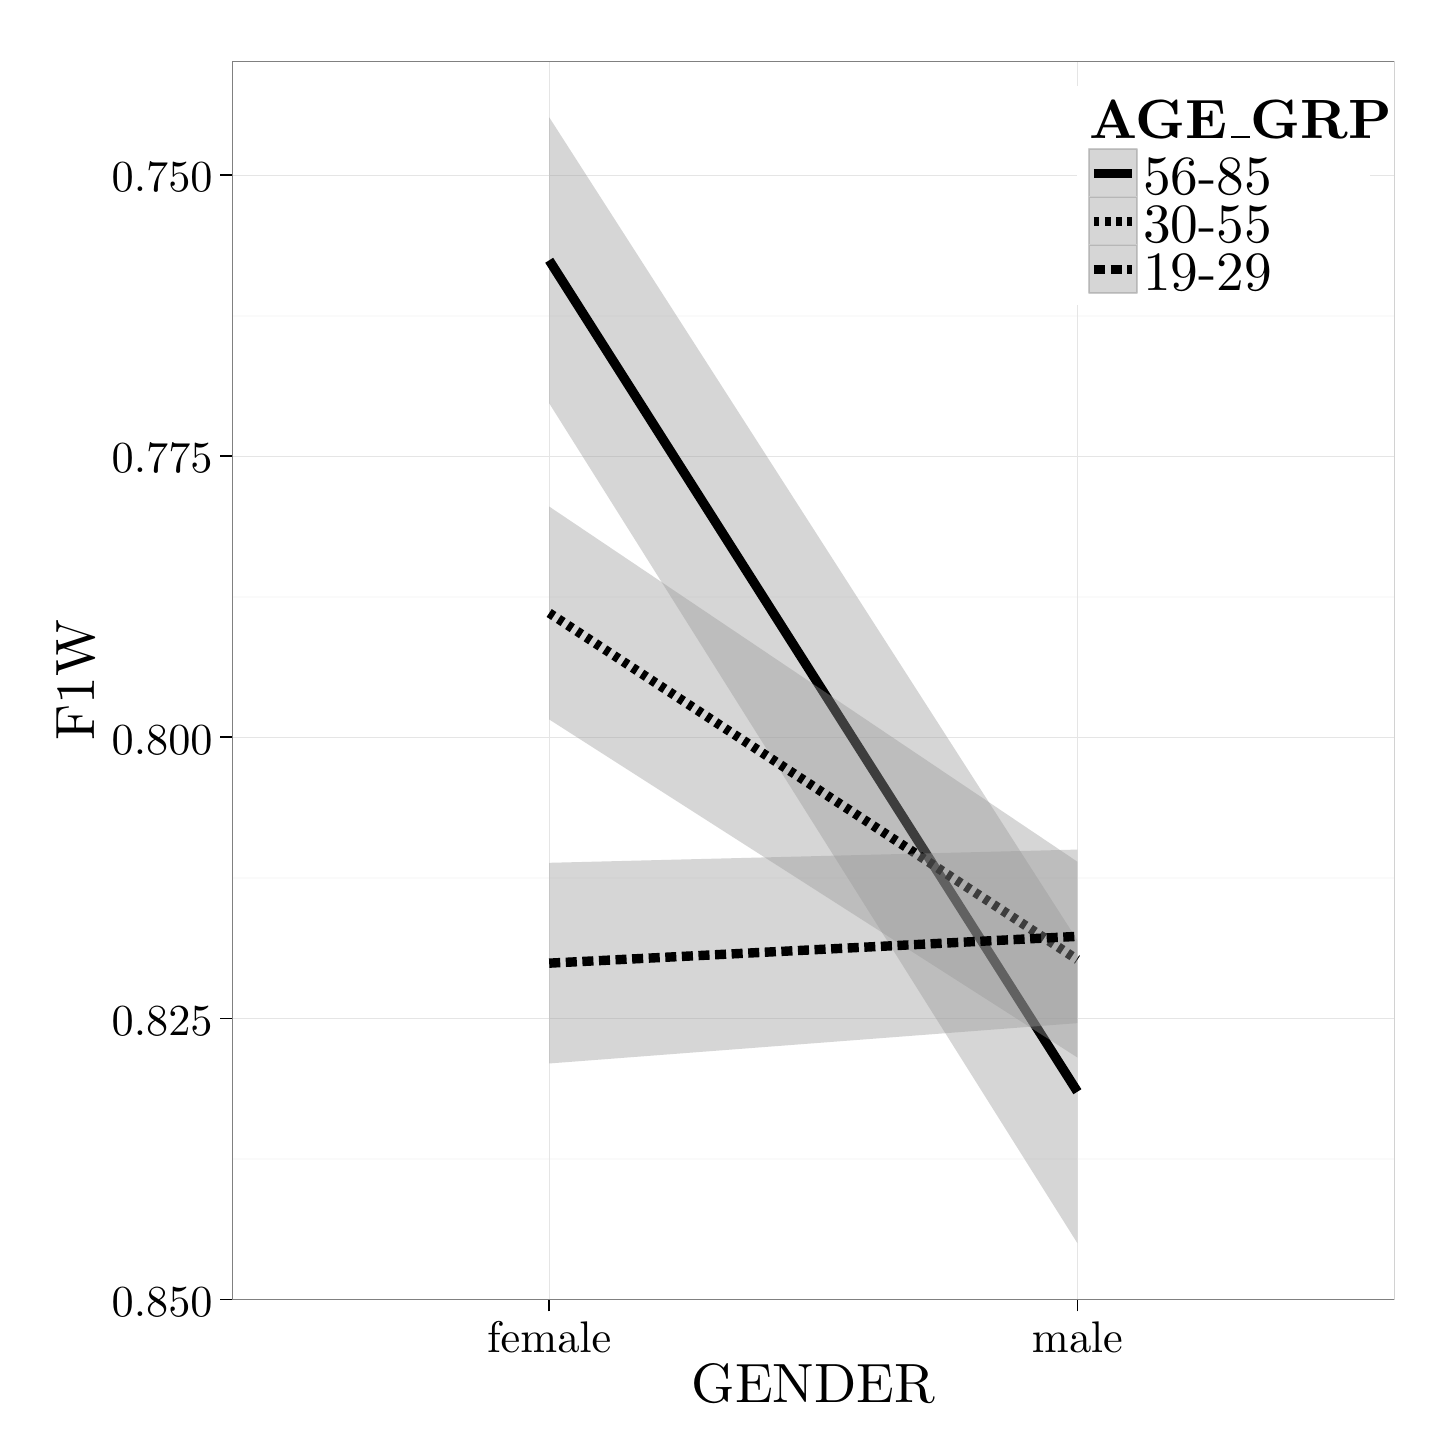
\begin{tikzpicture}[x=1pt,y=1pt]
\definecolor{fillColor}{RGB}{255,255,255}
\path[use as bounding box,fill=fillColor,fill opacity=0.00] (0,0) rectangle (505.89,505.89);
\begin{scope}
\path[clip] (  0.00,  0.00) rectangle (505.89,505.89);
\definecolor{drawColor}{RGB}{255,255,255}
\definecolor{fillColor}{RGB}{255,255,255}

\path[draw=drawColor,line width= 0.6pt,line join=round,line cap=round,fill=fillColor] (  0.00, -0.00) rectangle (505.89,505.89);
\end{scope}
\begin{scope}
\path[clip] ( 73.92, 46.31) rectangle (493.85,493.84);
\definecolor{fillColor}{RGB}{255,255,255}

\path[fill=fillColor] ( 73.92, 46.31) rectangle (493.85,493.84);
\definecolor{drawColor}{gray}{0.98}

\path[draw=drawColor,line width= 0.6pt,line join=round] ( 73.92,401.80) --
	(493.85,401.80);

\path[draw=drawColor,line width= 0.6pt,line join=round] ( 73.92,300.24) --
	(493.85,300.24);

\path[draw=drawColor,line width= 0.6pt,line join=round] ( 73.92,198.68) --
	(493.85,198.68);

\path[draw=drawColor,line width= 0.6pt,line join=round] ( 73.92, 97.11) --
	(493.85, 97.11);
\definecolor{drawColor}{gray}{0.90}

\path[draw=drawColor,line width= 0.2pt,line join=round] ( 73.92,452.58) --
	(493.85,452.58);

\path[draw=drawColor,line width= 0.2pt,line join=round] ( 73.92,351.02) --
	(493.85,351.02);

\path[draw=drawColor,line width= 0.2pt,line join=round] ( 73.92,249.46) --
	(493.85,249.46);

\path[draw=drawColor,line width= 0.2pt,line join=round] ( 73.92,147.90) --
	(493.85,147.90);

\path[draw=drawColor,line width= 0.2pt,line join=round] ( 73.92, 46.33) --
	(493.85, 46.33);

\path[draw=drawColor,line width= 0.2pt,line join=round] (188.45, 46.31) --
	(188.45,493.84);

\path[draw=drawColor,line width= 0.2pt,line join=round] (379.32, 46.31) --
	(379.32,493.84);
\definecolor{fillColor}{RGB}{153,153,153}

\path[fill=fillColor,fill opacity=0.40] (188.45,473.50) --
	(379.32,176.14) --
	(379.32, 66.65) --
	(188.45,370.16) --
	cycle;
\definecolor{drawColor}{RGB}{0,0,0}

\path[draw=drawColor,line width= 3.4pt,line join=round] (188.45,421.83) --
	(379.32,121.39);

\path[fill=fillColor,fill opacity=0.40] (188.45,332.85) --
	(379.32,204.50) --
	(379.32,133.75) --
	(188.45,255.91) --
	cycle;

\path[draw=drawColor,line width= 3.4pt,dash pattern=on 2pt off 2pt ,line join=round] (188.45,294.38) --
	(379.32,169.12);

\path[fill=fillColor,fill opacity=0.40] (188.45,204.11) --
	(379.32,208.89) --
	(379.32,146.18) --
	(188.45,131.60) --
	cycle;

\path[draw=drawColor,line width= 3.4pt,dash pattern=on 4pt off 2pt ,line join=round] (188.45,167.85) --
	(379.32,177.53);
\definecolor{drawColor}{gray}{0.50}

\path[draw=drawColor,line width= 0.6pt,line join=round,line cap=round] ( 73.92, 46.31) rectangle (493.85,493.84);
\end{scope}
\begin{scope}
\path[clip] (  0.00,  0.00) rectangle (505.89,505.89);
\definecolor{drawColor}{RGB}{0,0,0}

\node[text=drawColor,anchor=base east,inner sep=0pt, outer sep=0pt, scale=  1.60] at ( 66.81,446.55) {0.750};

\node[text=drawColor,anchor=base east,inner sep=0pt, outer sep=0pt, scale=  1.60] at ( 66.81,344.99) {0.775};

\node[text=drawColor,anchor=base east,inner sep=0pt, outer sep=0pt, scale=  1.60] at ( 66.81,243.42) {0.800};

\node[text=drawColor,anchor=base east,inner sep=0pt, outer sep=0pt, scale=  1.60] at ( 66.81,141.86) {0.825};

\node[text=drawColor,anchor=base east,inner sep=0pt, outer sep=0pt, scale=  1.60] at ( 66.81, 40.30) {0.850};
\end{scope}
\begin{scope}
\path[clip] (  0.00,  0.00) rectangle (505.89,505.89);
\definecolor{drawColor}{RGB}{0,0,0}

\path[draw=drawColor,line width= 0.6pt,line join=round] ( 69.66,452.58) --
	( 73.92,452.58);

\path[draw=drawColor,line width= 0.6pt,line join=round] ( 69.66,351.02) --
	( 73.92,351.02);

\path[draw=drawColor,line width= 0.6pt,line join=round] ( 69.66,249.46) --
	( 73.92,249.46);

\path[draw=drawColor,line width= 0.6pt,line join=round] ( 69.66,147.90) --
	( 73.92,147.90);

\path[draw=drawColor,line width= 0.6pt,line join=round] ( 69.66, 46.33) --
	( 73.92, 46.33);
\end{scope}
\begin{scope}
\path[clip] (  0.00,  0.00) rectangle (505.89,505.89);
\definecolor{drawColor}{RGB}{0,0,0}

\path[draw=drawColor,line width= 0.6pt,line join=round] (188.45, 42.04) --
	(188.45, 46.31);

\path[draw=drawColor,line width= 0.6pt,line join=round] (379.32, 42.04) --
	(379.32, 46.31);
\end{scope}
\begin{scope}
\path[clip] (  0.00,  0.00) rectangle (505.89,505.89);
\definecolor{drawColor}{RGB}{0,0,0}

\node[text=drawColor,anchor=base,inner sep=0pt, outer sep=0pt, scale=  1.60] at (188.45, 27.13) {female};

\node[text=drawColor,anchor=base,inner sep=0pt, outer sep=0pt, scale=  1.60] at (379.32, 27.13) {male};
\end{scope}
\begin{scope}
\path[clip] (  0.00,  0.00) rectangle (505.89,505.89);
\definecolor{drawColor}{RGB}{0,0,0}

\node[text=drawColor,anchor=base,inner sep=0pt, outer sep=0pt, scale=  2.00] at (283.88,  9.03) {GENDER};
\end{scope}
\begin{scope}
\path[clip] (  0.00,  0.00) rectangle (505.89,505.89);
\definecolor{drawColor}{RGB}{0,0,0}

\node[text=drawColor,rotate= 90.00,anchor=base,inner sep=0pt, outer sep=0pt, scale=  2.00] at ( 24.12,270.08) {F1W};
\end{scope}
\begin{scope}
\path[clip] (  0.00,  0.00) rectangle (505.89,505.89);
\definecolor{fillColor}{RGB}{255,255,255}

\path[fill=fillColor] (379.28,405.66) rectangle (484.98,484.98);
\end{scope}
\begin{scope}
\path[clip] (  0.00,  0.00) rectangle (505.89,505.89);
\definecolor{drawColor}{RGB}{0,0,0}

\node[text=drawColor,anchor=base west,inner sep=0pt, outer sep=0pt, scale=  2.00] at (383.55,465.96) {\bfseries AGE{\_{}}GRP};
\end{scope}
\begin{scope}
\path[clip] (  0.00,  0.00) rectangle (505.89,505.89);
\definecolor{drawColor}{gray}{0.80}
\definecolor{fillColor}{RGB}{255,255,255}

\path[draw=drawColor,line width= 0.6pt,line join=round,line cap=round,fill=fillColor] (383.55,444.61) rectangle (400.89,461.96);
\end{scope}
\begin{scope}
\path[clip] (  0.00,  0.00) rectangle (505.89,505.89);
\definecolor{fillColor}{RGB}{153,153,153}

\path[fill=fillColor,fill opacity=0.40] (383.55,444.61) rectangle (400.89,461.96);
\definecolor{drawColor}{RGB}{0,0,0}

\path[draw=drawColor,line width= 3.4pt,line join=round] (385.28,453.29) -- (399.16,453.29);
\end{scope}
\begin{scope}
\path[clip] (  0.00,  0.00) rectangle (505.89,505.89);
\definecolor{drawColor}{gray}{0.80}
\definecolor{fillColor}{RGB}{255,255,255}

\path[draw=drawColor,line width= 0.6pt,line join=round,line cap=round,fill=fillColor] (383.55,427.27) rectangle (400.89,444.61);
\end{scope}
\begin{scope}
\path[clip] (  0.00,  0.00) rectangle (505.89,505.89);
\definecolor{fillColor}{RGB}{153,153,153}

\path[fill=fillColor,fill opacity=0.40] (383.55,427.27) rectangle (400.89,444.61);
\definecolor{drawColor}{RGB}{0,0,0}

\path[draw=drawColor,line width= 3.4pt,dash pattern=on 2pt off 2pt ,line join=round] (385.28,435.94) -- (399.16,435.94);
\end{scope}
\begin{scope}
\path[clip] (  0.00,  0.00) rectangle (505.89,505.89);
\definecolor{drawColor}{gray}{0.80}
\definecolor{fillColor}{RGB}{255,255,255}

\path[draw=drawColor,line width= 0.6pt,line join=round,line cap=round,fill=fillColor] (383.55,409.92) rectangle (400.89,427.27);
\end{scope}
\begin{scope}
\path[clip] (  0.00,  0.00) rectangle (505.89,505.89);
\definecolor{fillColor}{RGB}{153,153,153}

\path[fill=fillColor,fill opacity=0.40] (383.55,409.92) rectangle (400.89,427.27);
\definecolor{drawColor}{RGB}{0,0,0}

\path[draw=drawColor,line width= 3.4pt,dash pattern=on 4pt off 2pt ,line join=round] (385.28,418.60) -- (399.16,418.60);
\end{scope}
\begin{scope}
\path[clip] (  0.00,  0.00) rectangle (505.89,505.89);
\definecolor{drawColor}{RGB}{0,0,0}

\node[text=drawColor,anchor=base west,inner sep=0pt, outer sep=0pt, scale=  2.00] at (403.06,445.75) {56-85};
\end{scope}
\begin{scope}
\path[clip] (  0.00,  0.00) rectangle (505.89,505.89);
\definecolor{drawColor}{RGB}{0,0,0}

\node[text=drawColor,anchor=base west,inner sep=0pt, outer sep=0pt, scale=  2.00] at (403.06,428.40) {30-55};
\end{scope}
\begin{scope}
\path[clip] (  0.00,  0.00) rectangle (505.89,505.89);
\definecolor{drawColor}{RGB}{0,0,0}

\node[text=drawColor,anchor=base west,inner sep=0pt, outer sep=0pt, scale=  2.00] at (403.06,411.06) {19-29};
\end{scope}
\end{tikzpicture}
} 
		\caption{regression plot}
		\label{fig.scatter.f1w.happy.genderage}
	\end{subfigure}
	\caption{happ\textsc{y} (F1) by gender and age}
\end{figure}

Just as in the case of the gender X social class interaction, the differences in slope of the three regression lines (steep fall for the oldest, moderate fall for the middle-aged, and ever so slight rise in the youngest group) also suggest that, conversely, gender differences are not equally pronounced in the different age groups.
Indeed, Figure \ref{fig.box.f1w.happy.genderage} shows that there is a quite pronounced difference between men and women in the oldest group, with the former having significantly lower realisations than the women (t(896.946) = -7.773, p < 0.001).
This difference is still present in the middle group (t(1955.552) = -4.707, p < 0.001), although the distance has clearly decreased.
For the youngest speakers, finally, there is no longer a significant difference between male and female speakers (t(1606.076) = 0.411, p = 0.681).
It is interesting that men do not seem to have changed much across these three generations; their means are comparatively similar.
Women, on the other hand, appear to have adapted to the men over time by lowering their originally higher happ\textsc{y} realisation to one that is almost identical to that of men.

\subsubsection{Style shifting}
\label{sec.prod.res.vow.happy.f1.shifting}

The last factor that turned up as a significant fixed effect in the regression model is style, the variable which this study is most interested in (though closely followed by age) because \isi{style shifting} is considered as an epiphenomenon of \isi{salience}.
Figure \ref{fig.line.f1w.happy.tot} represents the style dimension along the x-axis, starting with the word list on the left and going through the reading passage and free, spontaneous speech to the accent imitation\is{accent performance} task on the right of the graph.
F1 is, as usual, marked on the y-axis, while line type once again codes the three age groups of speakers.
The size of the whiskers corresponds to the standard error for each register and age group.

\begin{figure}[h!]
	\centering
		\definecolor{shadecolor}{rgb}{0.969, 0.969, 0.969}
		\resizebox{0.5\linewidth}{!}{% Created by tikzDevice version 0.8.1 on 2016-02-09 02:13:27
% !TEX encoding = UTF-8 Unicode
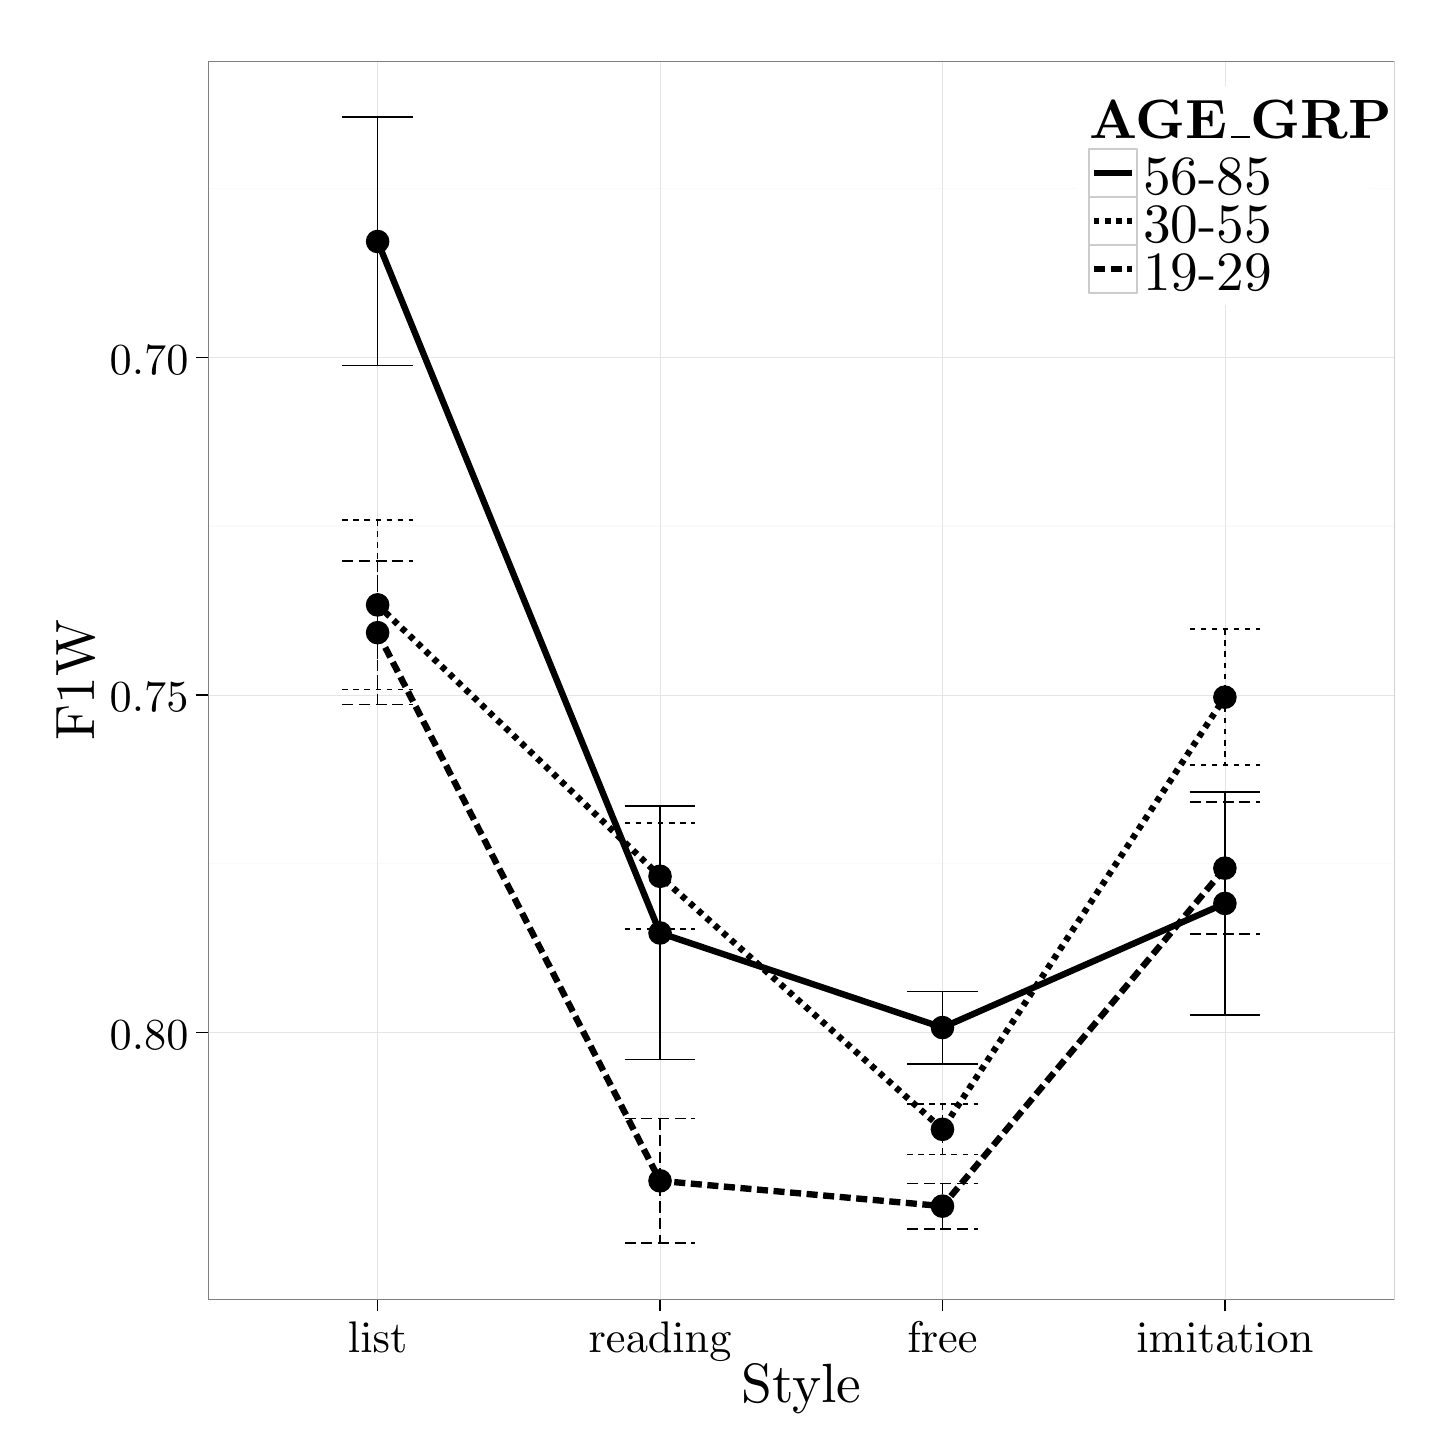
\begin{tikzpicture}[x=1pt,y=1pt]
\definecolor{fillColor}{RGB}{255,255,255}
\path[use as bounding box,fill=fillColor,fill opacity=0.00] (0,0) rectangle (505.89,505.89);
\begin{scope}
\path[clip] (  0.00,  0.00) rectangle (505.89,505.89);
\definecolor{drawColor}{RGB}{255,255,255}
\definecolor{fillColor}{RGB}{255,255,255}

\path[draw=drawColor,line width= 0.6pt,line join=round,line cap=round,fill=fillColor] (  0.00, -0.00) rectangle (505.89,505.89);
\end{scope}
\begin{scope}
\path[clip] ( 65.21, 46.31) rectangle (493.85,493.84);
\definecolor{fillColor}{RGB}{255,255,255}

\path[fill=fillColor] ( 65.21, 46.31) rectangle (493.85,493.84);
\definecolor{drawColor}{gray}{0.98}

\path[draw=drawColor,line width= 0.6pt,line join=round] ( 65.21,447.74) --
	(493.85,447.74);

\path[draw=drawColor,line width= 0.6pt,line join=round] ( 65.21,325.79) --
	(493.85,325.79);

\path[draw=drawColor,line width= 0.6pt,line join=round] ( 65.21,203.83) --
	(493.85,203.83);
\definecolor{drawColor}{gray}{0.90}

\path[draw=drawColor,line width= 0.2pt,line join=round] ( 65.21,386.76) --
	(493.85,386.76);

\path[draw=drawColor,line width= 0.2pt,line join=round] ( 65.21,264.81) --
	(493.85,264.81);

\path[draw=drawColor,line width= 0.2pt,line join=round] ( 65.21,142.85) --
	(493.85,142.85);

\path[draw=drawColor,line width= 0.2pt,line join=round] (126.45, 46.31) --
	(126.45,493.84);

\path[draw=drawColor,line width= 0.2pt,line join=round] (228.50, 46.31) --
	(228.50,493.84);

\path[draw=drawColor,line width= 0.2pt,line join=round] (330.56, 46.31) --
	(330.56,493.84);

\path[draw=drawColor,line width= 0.2pt,line join=round] (432.61, 46.31) --
	(432.61,493.84);
\definecolor{fillColor}{RGB}{0,0,0}

\path[fill=fillColor] (126.45,428.62) circle (  4.27);

\path[fill=fillColor] (126.45,297.31) circle (  4.27);

\path[fill=fillColor] (126.45,287.28) circle (  4.27);

\path[fill=fillColor] (228.50,178.76) circle (  4.27);

\path[fill=fillColor] (228.50,199.24) circle (  4.27);

\path[fill=fillColor] (228.50, 89.19) circle (  4.27);

\path[fill=fillColor] (330.56,144.58) circle (  4.27);

\path[fill=fillColor] (330.56,107.81) circle (  4.27);

\path[fill=fillColor] (330.56, 80.05) circle (  4.27);

\path[fill=fillColor] (432.61,189.43) circle (  4.27);

\path[fill=fillColor] (432.61,263.96) circle (  4.27);

\path[fill=fillColor] (432.61,202.18) circle (  4.27);
\definecolor{drawColor}{RGB}{0,0,0}

\path[draw=drawColor,line width= 2.3pt,line join=round] (126.45,428.62) --
	(228.50,178.76) --
	(330.56,144.58) --
	(432.61,189.43);

\path[draw=drawColor,line width= 2.3pt,dash pattern=on 2pt off 2pt ,line join=round] (126.45,297.31) --
	(228.50,199.24) --
	(330.56,107.81) --
	(432.61,263.96);

\path[draw=drawColor,line width= 2.3pt,dash pattern=on 4pt off 2pt ,line join=round] (126.45,287.28) --
	(228.50, 89.19) --
	(330.56, 80.05) --
	(432.61,202.18);

\path[draw=drawColor,line width= 0.6pt,line join=round] (113.69,473.50) --
	(139.20,473.50);

\path[draw=drawColor,line width= 0.6pt,line join=round] (126.45,473.50) --
	(126.45,383.75);

\path[draw=drawColor,line width= 0.6pt,line join=round] (113.69,383.75) --
	(139.20,383.75);

\path[draw=drawColor,line width= 0.6pt,line join=round] (215.75,224.52) --
	(241.26,224.52);

\path[draw=drawColor,line width= 0.6pt,line join=round] (228.50,224.52) --
	(228.50,133.00);

\path[draw=drawColor,line width= 0.6pt,line join=round] (215.75,133.00) --
	(241.26,133.00);

\path[draw=drawColor,line width= 0.6pt,line join=round] (317.80,157.67) --
	(343.31,157.67);

\path[draw=drawColor,line width= 0.6pt,line join=round] (330.56,157.67) --
	(330.56,131.49);

\path[draw=drawColor,line width= 0.6pt,line join=round] (317.80,131.49) --
	(343.31,131.49);

\path[draw=drawColor,line width= 0.6pt,line join=round] (419.86,229.76) --
	(445.37,229.76);

\path[draw=drawColor,line width= 0.6pt,line join=round] (432.61,229.76) --
	(432.61,149.10);

\path[draw=drawColor,line width= 0.6pt,line join=round] (419.86,149.10) --
	(445.37,149.10);

\path[draw=drawColor,line width= 0.6pt,dash pattern=on 2pt off 2pt ,line join=round] (113.69,327.93) --
	(139.20,327.93);

\path[draw=drawColor,line width= 0.6pt,dash pattern=on 2pt off 2pt ,line join=round] (126.45,327.93) --
	(126.45,266.68);

\path[draw=drawColor,line width= 0.6pt,dash pattern=on 2pt off 2pt ,line join=round] (113.69,266.68) --
	(139.20,266.68);

\path[draw=drawColor,line width= 0.6pt,dash pattern=on 2pt off 2pt ,line join=round] (215.75,218.39) --
	(241.26,218.39);

\path[draw=drawColor,line width= 0.6pt,dash pattern=on 2pt off 2pt ,line join=round] (228.50,218.39) --
	(228.50,180.09);

\path[draw=drawColor,line width= 0.6pt,dash pattern=on 2pt off 2pt ,line join=round] (215.75,180.09) --
	(241.26,180.09);

\path[draw=drawColor,line width= 0.6pt,dash pattern=on 2pt off 2pt ,line join=round] (317.80,116.91) --
	(343.31,116.91);

\path[draw=drawColor,line width= 0.6pt,dash pattern=on 2pt off 2pt ,line join=round] (330.56,116.91) --
	(330.56, 98.71);

\path[draw=drawColor,line width= 0.6pt,dash pattern=on 2pt off 2pt ,line join=round] (317.80, 98.71) --
	(343.31, 98.71);

\path[draw=drawColor,line width= 0.6pt,dash pattern=on 2pt off 2pt ,line join=round] (419.86,288.49) --
	(445.37,288.49);

\path[draw=drawColor,line width= 0.6pt,dash pattern=on 2pt off 2pt ,line join=round] (432.61,288.49) --
	(432.61,239.42);

\path[draw=drawColor,line width= 0.6pt,dash pattern=on 2pt off 2pt ,line join=round] (419.86,239.42) --
	(445.37,239.42);

\path[draw=drawColor,line width= 0.6pt,dash pattern=on 4pt off 2pt ,line join=round] (113.69,313.27) --
	(139.20,313.27);

\path[draw=drawColor,line width= 0.6pt,dash pattern=on 4pt off 2pt ,line join=round] (126.45,313.27) --
	(126.45,261.29);

\path[draw=drawColor,line width= 0.6pt,dash pattern=on 4pt off 2pt ,line join=round] (113.69,261.29) --
	(139.20,261.29);

\path[draw=drawColor,line width= 0.6pt,dash pattern=on 4pt off 2pt ,line join=round] (215.75,111.74) --
	(241.26,111.74);

\path[draw=drawColor,line width= 0.6pt,dash pattern=on 4pt off 2pt ,line join=round] (228.50,111.74) --
	(228.50, 66.65);

\path[draw=drawColor,line width= 0.6pt,dash pattern=on 4pt off 2pt ,line join=round] (215.75, 66.65) --
	(241.26, 66.65);

\path[draw=drawColor,line width= 0.6pt,dash pattern=on 4pt off 2pt ,line join=round] (317.80, 88.26) --
	(343.31, 88.26);

\path[draw=drawColor,line width= 0.6pt,dash pattern=on 4pt off 2pt ,line join=round] (330.56, 88.26) --
	(330.56, 71.83);

\path[draw=drawColor,line width= 0.6pt,dash pattern=on 4pt off 2pt ,line join=round] (317.80, 71.83) --
	(343.31, 71.83);

\path[draw=drawColor,line width= 0.6pt,dash pattern=on 4pt off 2pt ,line join=round] (419.86,226.08) --
	(445.37,226.08);

\path[draw=drawColor,line width= 0.6pt,dash pattern=on 4pt off 2pt ,line join=round] (432.61,226.08) --
	(432.61,178.29);

\path[draw=drawColor,line width= 0.6pt,dash pattern=on 4pt off 2pt ,line join=round] (419.86,178.29) --
	(445.37,178.29);
\definecolor{drawColor}{gray}{0.50}

\path[draw=drawColor,line width= 0.6pt,line join=round,line cap=round] ( 65.21, 46.31) rectangle (493.85,493.84);
\end{scope}
\begin{scope}
\path[clip] (  0.00,  0.00) rectangle (505.89,505.89);
\definecolor{drawColor}{RGB}{0,0,0}

\node[text=drawColor,anchor=base east,inner sep=0pt, outer sep=0pt, scale=  1.60] at ( 58.10,380.73) {0.70};

\node[text=drawColor,anchor=base east,inner sep=0pt, outer sep=0pt, scale=  1.60] at ( 58.10,258.78) {0.75};

\node[text=drawColor,anchor=base east,inner sep=0pt, outer sep=0pt, scale=  1.60] at ( 58.10,136.82) {0.80};
\end{scope}
\begin{scope}
\path[clip] (  0.00,  0.00) rectangle (505.89,505.89);
\definecolor{drawColor}{RGB}{0,0,0}

\path[draw=drawColor,line width= 0.6pt,line join=round] ( 60.95,386.76) --
	( 65.21,386.76);

\path[draw=drawColor,line width= 0.6pt,line join=round] ( 60.95,264.81) --
	( 65.21,264.81);

\path[draw=drawColor,line width= 0.6pt,line join=round] ( 60.95,142.85) --
	( 65.21,142.85);
\end{scope}
\begin{scope}
\path[clip] (  0.00,  0.00) rectangle (505.89,505.89);
\definecolor{drawColor}{RGB}{0,0,0}

\path[draw=drawColor,line width= 0.6pt,line join=round] (126.45, 42.04) --
	(126.45, 46.31);

\path[draw=drawColor,line width= 0.6pt,line join=round] (228.50, 42.04) --
	(228.50, 46.31);

\path[draw=drawColor,line width= 0.6pt,line join=round] (330.56, 42.04) --
	(330.56, 46.31);

\path[draw=drawColor,line width= 0.6pt,line join=round] (432.61, 42.04) --
	(432.61, 46.31);
\end{scope}
\begin{scope}
\path[clip] (  0.00,  0.00) rectangle (505.89,505.89);
\definecolor{drawColor}{RGB}{0,0,0}

\node[text=drawColor,anchor=base,inner sep=0pt, outer sep=0pt, scale=  1.60] at (126.45, 27.13) {list};

\node[text=drawColor,anchor=base,inner sep=0pt, outer sep=0pt, scale=  1.60] at (228.50, 27.13) {reading};

\node[text=drawColor,anchor=base,inner sep=0pt, outer sep=0pt, scale=  1.60] at (330.56, 27.13) {free};

\node[text=drawColor,anchor=base,inner sep=0pt, outer sep=0pt, scale=  1.60] at (432.61, 27.13) {imitation};
\end{scope}
\begin{scope}
\path[clip] (  0.00,  0.00) rectangle (505.89,505.89);
\definecolor{drawColor}{RGB}{0,0,0}

\node[text=drawColor,anchor=base,inner sep=0pt, outer sep=0pt, scale=  2.00] at (279.53,  9.03) {Style};
\end{scope}
\begin{scope}
\path[clip] (  0.00,  0.00) rectangle (505.89,505.89);
\definecolor{drawColor}{RGB}{0,0,0}

\node[text=drawColor,rotate= 90.00,anchor=base,inner sep=0pt, outer sep=0pt, scale=  2.00] at ( 24.12,270.08) {F1W};
\end{scope}
\begin{scope}
\path[clip] (  0.00,  0.00) rectangle (505.89,505.89);
\definecolor{fillColor}{RGB}{255,255,255}

\path[fill=fillColor] (379.28,405.66) rectangle (484.98,484.98);
\end{scope}
\begin{scope}
\path[clip] (  0.00,  0.00) rectangle (505.89,505.89);
\definecolor{drawColor}{RGB}{0,0,0}

\node[text=drawColor,anchor=base west,inner sep=0pt, outer sep=0pt, scale=  2.00] at (383.55,465.96) {\bfseries AGE{\_{}}GRP};
\end{scope}
\begin{scope}
\path[clip] (  0.00,  0.00) rectangle (505.89,505.89);
\definecolor{drawColor}{gray}{0.80}
\definecolor{fillColor}{RGB}{255,255,255}

\path[draw=drawColor,line width= 0.6pt,line join=round,line cap=round,fill=fillColor] (383.55,444.61) rectangle (400.89,461.96);
\end{scope}
\begin{scope}
\path[clip] (  0.00,  0.00) rectangle (505.89,505.89);
\definecolor{drawColor}{RGB}{0,0,0}

\path[draw=drawColor,line width= 2.3pt,line join=round] (385.28,453.29) -- (399.16,453.29);
\end{scope}
\begin{scope}
\path[clip] (  0.00,  0.00) rectangle (505.89,505.89);
\definecolor{drawColor}{RGB}{0,0,0}

\path[draw=drawColor,line width= 0.6pt,line join=round] (385.28,453.29) -- (399.16,453.29);
\end{scope}
\begin{scope}
\path[clip] (  0.00,  0.00) rectangle (505.89,505.89);
\definecolor{drawColor}{gray}{0.80}
\definecolor{fillColor}{RGB}{255,255,255}

\path[draw=drawColor,line width= 0.6pt,line join=round,line cap=round,fill=fillColor] (383.55,427.27) rectangle (400.89,444.61);
\end{scope}
\begin{scope}
\path[clip] (  0.00,  0.00) rectangle (505.89,505.89);
\definecolor{drawColor}{RGB}{0,0,0}

\path[draw=drawColor,line width= 2.3pt,dash pattern=on 2pt off 2pt ,line join=round] (385.28,435.94) -- (399.16,435.94);
\end{scope}
\begin{scope}
\path[clip] (  0.00,  0.00) rectangle (505.89,505.89);
\definecolor{drawColor}{RGB}{0,0,0}

\path[draw=drawColor,line width= 0.6pt,dash pattern=on 2pt off 2pt ,line join=round] (385.28,435.94) -- (399.16,435.94);
\end{scope}
\begin{scope}
\path[clip] (  0.00,  0.00) rectangle (505.89,505.89);
\definecolor{drawColor}{gray}{0.80}
\definecolor{fillColor}{RGB}{255,255,255}

\path[draw=drawColor,line width= 0.6pt,line join=round,line cap=round,fill=fillColor] (383.55,409.92) rectangle (400.89,427.27);
\end{scope}
\begin{scope}
\path[clip] (  0.00,  0.00) rectangle (505.89,505.89);
\definecolor{drawColor}{RGB}{0,0,0}

\path[draw=drawColor,line width= 2.3pt,dash pattern=on 4pt off 2pt ,line join=round] (385.28,418.60) -- (399.16,418.60);
\end{scope}
\begin{scope}
\path[clip] (  0.00,  0.00) rectangle (505.89,505.89);
\definecolor{drawColor}{RGB}{0,0,0}

\path[draw=drawColor,line width= 0.6pt,dash pattern=on 4pt off 2pt ,line join=round] (385.28,418.60) -- (399.16,418.60);
\end{scope}
\begin{scope}
\path[clip] (  0.00,  0.00) rectangle (505.89,505.89);
\definecolor{drawColor}{RGB}{0,0,0}

\node[text=drawColor,anchor=base west,inner sep=0pt, outer sep=0pt, scale=  2.00] at (403.06,445.75) {56-85};
\end{scope}
\begin{scope}
\path[clip] (  0.00,  0.00) rectangle (505.89,505.89);
\definecolor{drawColor}{RGB}{0,0,0}

\node[text=drawColor,anchor=base west,inner sep=0pt, outer sep=0pt, scale=  2.00] at (403.06,428.40) {30-55};
\end{scope}
\begin{scope}
\path[clip] (  0.00,  0.00) rectangle (505.89,505.89);
\definecolor{drawColor}{RGB}{0,0,0}

\node[text=drawColor,anchor=base west,inner sep=0pt, outer sep=0pt, scale=  2.00] at (403.06,411.06) {19-29};
\end{scope}
\end{tikzpicture}
} 
	\caption{happ\textsc{y} (F1) by age and style}
	\label{fig.line.f1w.happy.tot}
\end{figure}

The crucial question now is whether we are looking at \isi{style shifting} or not.
Productions of happ\textsc{y}, across age groups, are higher in the `list' register than when subjects read out a text.
These differences are visibly significant because the whiskers of the `list' and `reading' categories do not overlap for any of the age groups.
From the reading passage to spontaneous speech happ\textsc{y} seems to get even lower, but this is only significant in the middle-aged group.
Both the whiskers attached to the solid (old speakers) and the dashed (young speakers) dots overlap for these two registers.
Realisations during the accent perform\is{accent performance}ance are then higher again, though not as high as when reading a word list (the rise is non-significant for the oldest speakers in the sample).
Older speakers thus only distinguish the word list style from the other three (which do not differ significantly), middle-aged subjects have similar realisations for the word list and the accent perform\is{accent performance}ance, and the youngest interviewees distinguish reading and spontaneous speech together from both imitation\is{accent performance} and the word list.

These slightly different tendencies in the three age groups are not pronounced enough to show up as a significant interaction of age group and style in the mixed linear effects regression.
Judging from Figure \ref{fig.line.f1w.happy.tot}, this is probably not too surprising because there does seem to be a similar trend across the age groups even if the differences are not all equally significant.
The pattern that we see is not really one of `classical' \isi{style shifting}, though.
Instead of a steady decline from the most formal to the most informal speech style, a sort of U- or V-shaped pattern emerges.
In this context, it seems worthwhile to consider an explanation based on phonetic aspects, more precisely on duration.
Table \ref{tab.dur.style.happy} reports mean durations of happ\textsc{y} (in milliseconds), and mean \isi{frequency} scores of carrier words for each style and in each age group.

\begin{table}[h!]
	\centering
	\caption{happ\textsc{y}: durations (ms) and frequency (Zipf scores) by style and age}
	\label{tab.dur.style.happy}
	\begin{tabular}{lrrrrrrrr}
		\hline
		& \multicolumn{2}{c}{list} & \multicolumn{2}{c}{reading} & \multicolumn{2}{c}{free} & \multicolumn{2}{c}{imitation\is{accent performance}}\\
		& dur. & freq. & dur. & freq. & dur. & freq. & dur. & freq.\\
		\hline
		old & 90.20 & 4.69 & 64.30 & 4.46 & 68.16 & 5.10 & 69.31 & 4.34\\
		middle & 90.82 & 4.72 & 62.70 & 4.46 & 62.94 & 5.23 & 62.13 & 4.51\\
		young & 104.07 & 4.69 & 62.72 & 4.41 & 65.36 & 5.37 & 55.94 & 4.43\\
		\hline
	\end{tabular}
\end{table}

As is to be expected, \isi{vowel duration}s are, on average, considerably longer when people read out a word list.
Longer \isi{vowel duration}s, in turn, favour more peripheral happ\textsc{y} realisations, as has been shown (and explained) above.
At least in parts, the higher variants in the word list can thus be explained simply by the fact that they are also longer.
It is clear, however, that this is only part of the story, and that some sub-conscious\is{awareness} shifting must be involved as well, because \isi{vowel duration}s are comparable (and certainly not considerably longer) during accent imitation\is{accent performance}, text reading, and free speech.
Higher, more Scouse realisations when perform\is{accent performance}ing the accent can therefore not be explained by a phonetic effect of longer \isi{vowel duration}s.
The same seems to hold, more or less, for \isi{frequency} of the carrier word as well: more frequent words, on average, are used in spontaneous speech (which could go some way to explaining lower realisations in this register), but in the other three styles frequencies are very similar, despite the fact that F1 values are not.
A possible explanation that goes beyond duration and \isi{frequency} will be discussed in Chapter \ref{ch.prod_discussion}.

\subsection{F2 (happ\textsc{y})}
\label{sec.prod.res.vow.happy.f2}

\subsubsection{Overview}
\label{sec.prod.res.vow.happy.f2.overview}

Since the maximal model for happ\textsc{y} F2 measurements was based on exactly the same dataset as the one where the dependent variable was F1, the same problems with \isi{collinearity} also emerged.
These were dealt with in an identical manner as has been described for the happ\textsc{y} F1 model.
In the end, interactions were likewise re-entered into the regression and model selection based on AIC scores and F-tests comparing nested models resulted in the minimal adequate model printed as Table \ref{tab.regression.happy.f2} (R\textsuperscript{2}-equivalent = 0.268).

{
	\footnotesize
	\begin{longtable}[c]{p{0.3\textwidth}rrrrrl}
		\caption{happ\textsc{y} (F2): mixed linear effects regression}\label{tab.regression.happy.f2}\\

		\hline
		Fixed effects: & Estimate & Std. Error & df & t value & Pr($>$$|$t$|$) & \\ 
		\hline
		(Intercept) & 1.64 & 0.02 & 656.54 & 75.97 & < 0.001 & *** \\ 
		STYLElist & 0.10 & 0.05 & 1799.79 & 1.98 & 0.05 & *\\ 
		STYLEread & -0.05 & 0.02 & 1638.38 & -2.55 & 0.01 & *\\ 
		STYLEfree & -0.04 & 0.02 & 1501.28 & -2.09 & 0.04 & *\\ 
		AGE56-85 & 0.03 & 0.02 & 1959.22 & 1.41 & 0.16 & \\ 
		AGE30-55 & 0.01 & 0.02 & 1947.73 & 0.36 & 0.72 & \\ 
		GENDERf & 0.02 & 0.00 & 2079.61 & 6.38 & < 0.001 & *** \\ 
		CLASSmc & -0.01 & 0.00 & 2081.99 & -1.88 & 0.06 & .\\ 
		DURATION & 0.00 & 0.00 & 2070.57 & 7.80 & < 0.001 & *** \\ 
		PREMANNERaffr & 0.00 & 0.04 & 115.37 & 0.01 & 1.00 & \\ 
		PREMANNERfric & 0.05 & 0.02 & 125.52 & 2.19 & 0.03 & *\\ 
		PREMANNERliq & -0.04 & 0.01 & 114.24 & -3.22 & < 0.01 & ** \\ 
		PREMANNERnas & -0.02 & 0.02 & 93.43 & -0.92 & 0.36 & \\ 
		POSTMANNERaffr & 0.06 & 0.02 & 2071.42 & 3.23 & < 0.01 & ** \\ 
		POSTMANNERfric & -0.01 & 0.01 & 2077.31 & -2.22 & 0.03 & * \\ 
		POSTMANNERgli & 0.00 & 0.01 & 2063.14 & 0.32 & 0.75 & \\ 
		POSTMANNERliq & -0.05 & 0.01 & 2025.37 & -5.72 & < 0.001 & *** \\ 
		POSTMANNERnas & 0.01 & 0.01 & 2067.51 & 0.69 & 0.49 & \\ 
		STYLElist:GENDERf & 0.09 & 0.02 & 1982.28 & 5.36 & < 0.001 & *** \\ 
		STYLEread:GENDERf & -0.03 & 0.01 & 1962.17 & -3.22 & < 0.01 & ** \\ 
		AGE56-85:CLASSmc & -0.01 & 0.00 & 2080.77 & -2.93 & < 0.01 & ** \\ 
		AGE30-55:CLASSmc & 0.01 & 0.00 & 2070.63 & 3.18 & < 0.01 & ** \\ 
		STYLEread:AGE56-85:GENDERf & -0.02 & 0.03 & 1950.17 & -0.54 & 0.59 & \\ 
		STYLEfree:AGE56-85:GENDERf & -0.03 & 0.02 & 1988.95 & -1.22 & 0.22 & \\ 
		STYLEimit:AGE56-85:GENDERf & -0.01 & 0.04 & 1945.32 & -0.34 & 0.74 & \\ 
		STYLEread:AGE30-55:GENDERf & -0.01 & 0.03 & 1945.26 & -0.22 & 0.82 & \\ 
		STYLEfree:AGE30-55:GENDERf & 0.01 & 0.02 & 1965.59 & 0.37 & 0.71 & \\ 
		STYLEimit:AGE30-55:GENDERf & 0.05 & 0.03 & 1944.32 & 1.61 & 0.11 & \\ 
		STYLElist:AGE56-85:GENDERm & -0.02 & 0.10 & 2063.72 & -0.19 & 0.85 & \\ 
		STYLEread:AGE56-85:GENDERm & 0.00 & 0.03 & 1949.44 & 0.07 & 0.95 & \\ 
		STYLEfree:AGE56-85:GENDERm & -0.04 & 0.02 & 1978.35 & -1.75 & 0.08 & .\\ 
		STYLElist:AGE30-55:GENDERm & 0.10 & 0.07 & 2081.56 & 1.39 & 0.17 & \\ 
		STYLEread:AGE30-55:GENDERm & -0.00 & 0.03 & 1942.75 & -0.08 & 0.94 & \\ 
		STYLEfree:AGE30-55:GENDERm & 0.04 & 0.02 & 1963.18 & 1.75 & 0.08 & .\\ 
		\hline
		Random effects: & \multicolumn{6}{l}{(number of obs: 2116, groups: WORD, 221)} \\
		Groups &         Name & Variance &      Std.Dev. & & & \\
		WORD &  (Intercept) & 0.002 & 0.043 & & & \\
		Residual  &         & 0.015 & 0.124 & & & \\
		\hline
	\end{longtable}
}

This minimal model is very similar to the one that was reported for F1 measurements.
Style and gender turn up as significant predictors again.
Age is not a significant main effect for F2 of happ\textsc{y}, but it does appear in a significant interaction of age and class.
Social class, in turn, just about fails to reach significance as a main effect at the 5\% level.
The second two-way interaction that was retained in the model is that of style and gender.
A three-way interaction of style, age, and gender did not reach significance, but was retained anyway because an \textsc{anova} revealed that eliminating it resulted in a significantly worse fit to the data.
With respect to the non-social predictors there are some changes as well.
Vowel duration is, once more, highly significant, but \isi{frequency} of the keyword does not seem to have a statistically robust impact on F2 measurements.
Contrary to the regression of F1, both the following \emph{and} the preceding consonant (or, rather, its manner of articulation) are significant fixed effects in this model.
These last two predictors will be briefly analysed first.

\subsubsection{Phonological context}
\label{sec.prod.res.vow.happy.f2.phon}

\begin{figure}[h!]
	\centering
	\begin{subfigure}{.49\textwidth}
		\centering
			\definecolor{shadecolor}{rgb}{0.969, 0.969, 0.969}
			\resizebox{\linewidth}{!}{% Created by tikzDevice version 0.8.1 on 2016-02-09 02:13:46
% !TEX encoding = UTF-8 Unicode
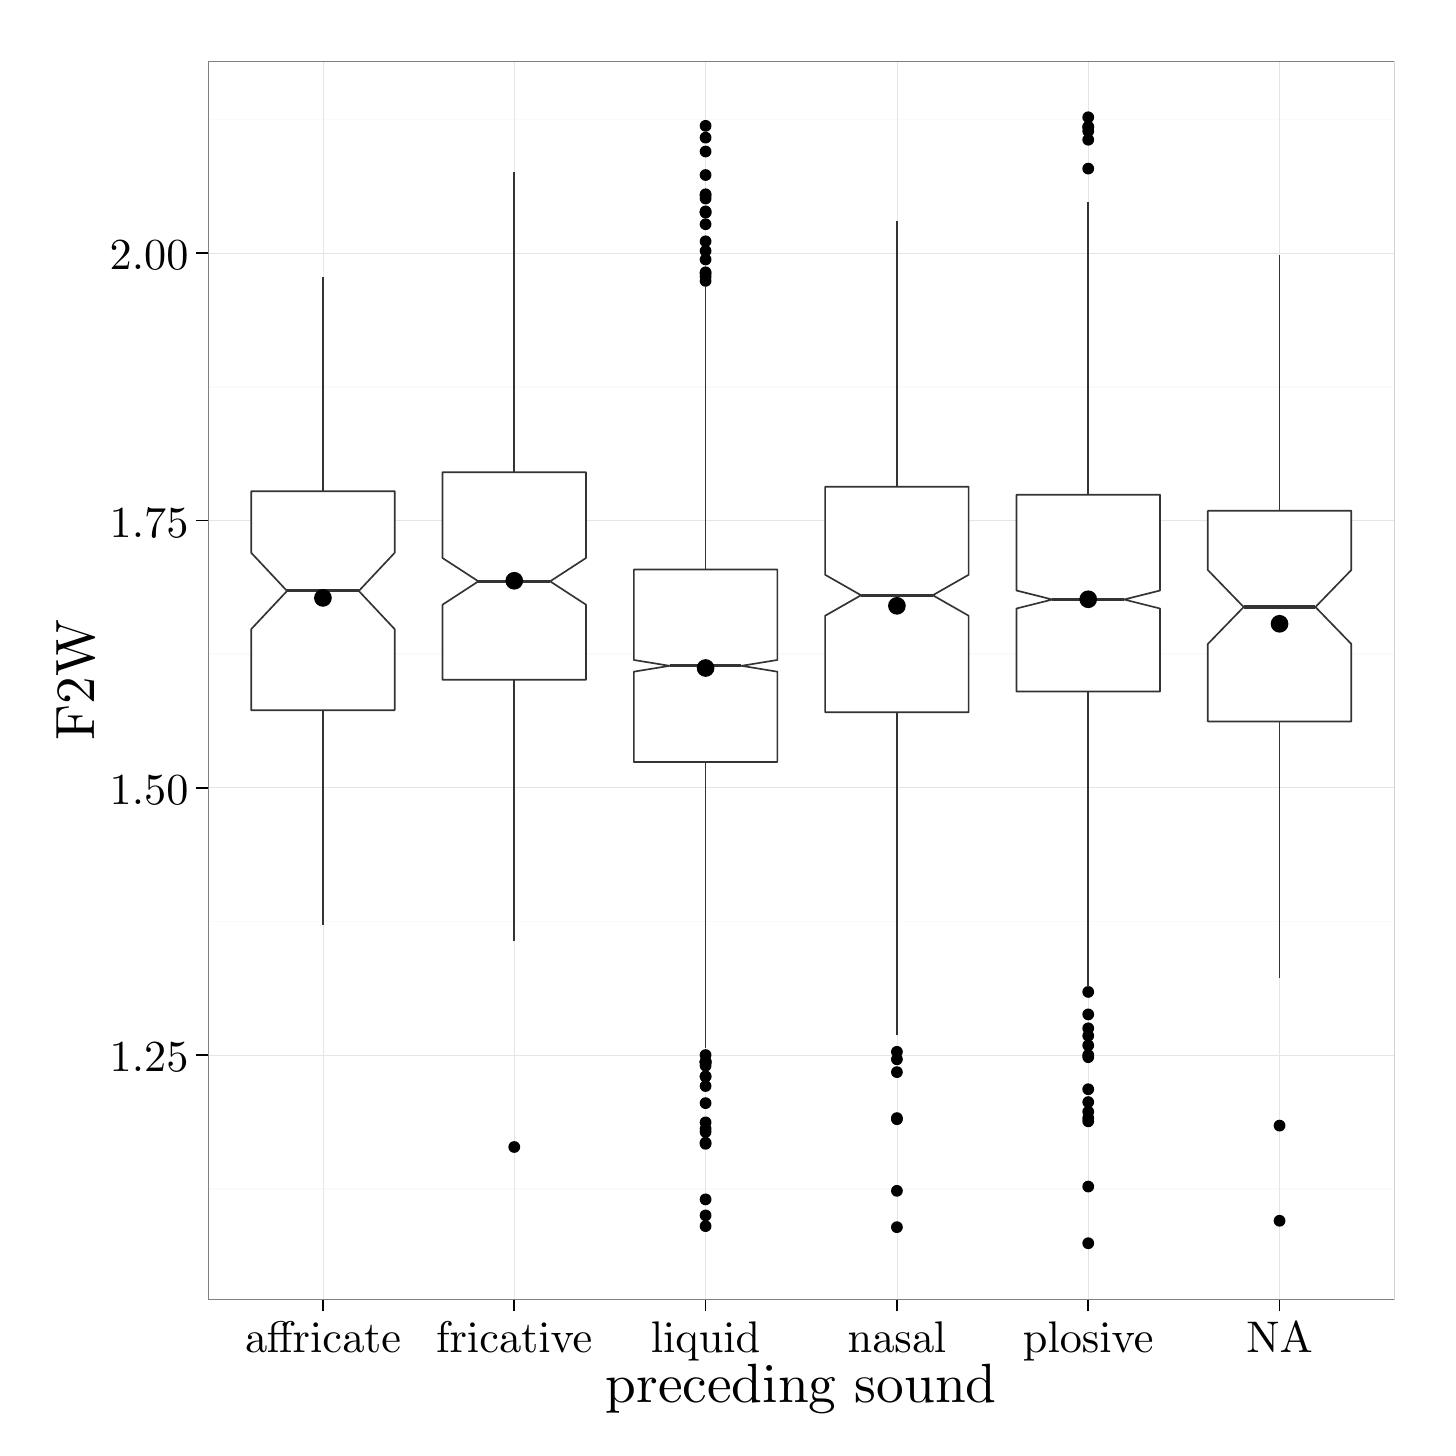
\begin{tikzpicture}[x=1pt,y=1pt]
\definecolor{fillColor}{RGB}{255,255,255}
\path[use as bounding box,fill=fillColor,fill opacity=0.00] (0,0) rectangle (505.89,505.89);
\begin{scope}
\path[clip] (  0.00,  0.00) rectangle (505.89,505.89);
\definecolor{drawColor}{RGB}{255,255,255}
\definecolor{fillColor}{RGB}{255,255,255}

\path[draw=drawColor,line width= 0.6pt,line join=round,line cap=round,fill=fillColor] (  0.00, -0.00) rectangle (505.89,505.89);
\end{scope}
\begin{scope}
\path[clip] ( 65.21, 46.31) rectangle (493.85,493.84);
\definecolor{fillColor}{RGB}{255,255,255}

\path[fill=fillColor] ( 65.21, 46.31) rectangle (493.85,493.84);
\definecolor{drawColor}{gray}{0.98}

\path[draw=drawColor,line width= 0.6pt,line join=round] ( 65.21, 86.36) --
	(493.85, 86.36);

\path[draw=drawColor,line width= 0.6pt,line join=round] ( 65.21,182.95) --
	(493.85,182.95);

\path[draw=drawColor,line width= 0.6pt,line join=round] ( 65.21,279.54) --
	(493.85,279.54);

\path[draw=drawColor,line width= 0.6pt,line join=round] ( 65.21,376.14) --
	(493.85,376.14);

\path[draw=drawColor,line width= 0.6pt,line join=round] ( 65.21,472.73) --
	(493.85,472.73);
\definecolor{drawColor}{gray}{0.90}

\path[draw=drawColor,line width= 0.2pt,line join=round] ( 65.21,134.65) --
	(493.85,134.65);

\path[draw=drawColor,line width= 0.2pt,line join=round] ( 65.21,231.25) --
	(493.85,231.25);

\path[draw=drawColor,line width= 0.2pt,line join=round] ( 65.21,327.84) --
	(493.85,327.84);

\path[draw=drawColor,line width= 0.2pt,line join=round] ( 65.21,424.43) --
	(493.85,424.43);

\path[draw=drawColor,line width= 0.2pt,line join=round] (106.69, 46.31) --
	(106.69,493.84);

\path[draw=drawColor,line width= 0.2pt,line join=round] (175.83, 46.31) --
	(175.83,493.84);

\path[draw=drawColor,line width= 0.2pt,line join=round] (244.96, 46.31) --
	(244.96,493.84);

\path[draw=drawColor,line width= 0.2pt,line join=round] (314.10, 46.31) --
	(314.10,493.84);

\path[draw=drawColor,line width= 0.2pt,line join=round] (383.23, 46.31) --
	(383.23,493.84);

\path[draw=drawColor,line width= 0.2pt,line join=round] (452.36, 46.31) --
	(452.36,493.84);
\definecolor{drawColor}{gray}{0.20}

\path[draw=drawColor,line width= 0.6pt,line join=round] (106.69,338.37) -- (106.69,415.93);

\path[draw=drawColor,line width= 0.6pt,line join=round] (106.69,259.26) -- (106.69,181.79);

\path[draw=drawColor,line width= 0.6pt,line join=round,line cap=round,fill=fillColor] ( 80.77,338.37) --
	( 80.77,316.14) --
	( 93.73,302.34) --
	( 80.77,288.54) --
	( 80.77,259.26) --
	(132.62,259.26) --
	(132.62,288.54) --
	(119.66,302.34) --
	(132.62,316.14) --
	(132.62,338.37) --
	( 80.77,338.37) --
	cycle;

\path[draw=drawColor,line width= 1.1pt,line join=round] ( 93.73,302.34) -- (119.66,302.34);
\definecolor{fillColor}{RGB}{0,0,0}

\path[fill=fillColor] (175.83,101.42) circle (  2.13);

\path[draw=drawColor,line width= 0.6pt,line join=round] (175.83,345.23) -- (175.83,453.80);

\path[draw=drawColor,line width= 0.6pt,line join=round] (175.83,270.27) -- (175.83,175.99);
\definecolor{fillColor}{RGB}{255,255,255}

\path[draw=drawColor,line width= 0.6pt,line join=round,line cap=round,fill=fillColor] (149.90,345.23) --
	(149.90,314.25) --
	(162.87,305.82) --
	(149.90,297.38) --
	(149.90,270.27) --
	(201.75,270.27) --
	(201.75,297.38) --
	(188.79,305.82) --
	(201.75,314.25) --
	(201.75,345.23) --
	(149.90,345.23) --
	cycle;

\path[draw=drawColor,line width= 1.1pt,line join=round] (162.87,305.82) -- (188.79,305.82);
\definecolor{fillColor}{RGB}{0,0,0}

\path[fill=fillColor] (244.96,132.33) circle (  2.13);

\path[fill=fillColor] (244.96,134.65) circle (  2.13);

\path[fill=fillColor] (244.96,110.31) circle (  2.13);

\path[fill=fillColor] (244.96,126.92) circle (  2.13);

\path[fill=fillColor] (244.96,107.99) circle (  2.13);

\path[fill=fillColor] (244.96,445.30) circle (  2.13);

\path[fill=fillColor] (244.96,425.21) circle (  2.13);

\path[fill=fillColor] (244.96,422.11) circle (  2.13);

\path[fill=fillColor] (244.96,132.33) circle (  2.13);

\path[fill=fillColor] (244.96,414.39) circle (  2.13);

\path[fill=fillColor] (244.96,434.86) circle (  2.13);

\path[fill=fillColor] (244.96,106.83) circle (  2.13);

\path[fill=fillColor] (244.96,439.12) circle (  2.13);

\path[fill=fillColor] (244.96,445.68) circle (  2.13);

\path[fill=fillColor] (244.96,439.12) circle (  2.13);

\path[fill=fillColor] (244.96,417.48) circle (  2.13);

\path[fill=fillColor] (244.96,439.50) circle (  2.13);

\path[fill=fillColor] (244.96,428.68) circle (  2.13);

\path[fill=fillColor] (244.96,452.64) circle (  2.13);

\path[fill=fillColor] (244.96,470.41) circle (  2.13);

\path[fill=fillColor] (244.96,444.14) circle (  2.13);

\path[fill=fillColor] (244.96,466.16) circle (  2.13);

\path[fill=fillColor] (244.96,117.27) circle (  2.13);

\path[fill=fillColor] (244.96,102.97) circle (  2.13);

\path[fill=fillColor] (244.96, 72.83) circle (  2.13);

\path[fill=fillColor] (244.96,131.95) circle (  2.13);

\path[fill=fillColor] (244.96,102.58) circle (  2.13);

\path[fill=fillColor] (244.96, 82.49) circle (  2.13);

\path[fill=fillColor] (244.96,131.95) circle (  2.13);

\path[fill=fillColor] (244.96, 76.70) circle (  2.13);

\path[fill=fillColor] (244.96,123.45) circle (  2.13);

\path[fill=fillColor] (244.96,417.09) circle (  2.13);

\path[fill=fillColor] (244.96,415.93) circle (  2.13);

\path[fill=fillColor] (244.96,130.79) circle (  2.13);

\path[fill=fillColor] (244.96,461.14) circle (  2.13);

\path[fill=fillColor] (244.96,126.92) circle (  2.13);

\path[draw=drawColor,line width= 0.6pt,line join=round] (244.96,310.07) -- (244.96,412.07);

\path[draw=drawColor,line width= 0.6pt,line join=round] (244.96,240.52) -- (244.96,137.36);
\definecolor{fillColor}{RGB}{255,255,255}

\path[draw=drawColor,line width= 0.6pt,line join=round,line cap=round,fill=fillColor] (219.04,310.07) --
	(219.04,277.40) --
	(232.00,275.29) --
	(219.04,273.18) --
	(219.04,240.52) --
	(270.89,240.52) --
	(270.89,273.18) --
	(257.93,275.29) --
	(270.89,277.40) --
	(270.89,310.07) --
	(219.04,310.07) --
	cycle;

\path[draw=drawColor,line width= 1.1pt,line join=round] (232.00,275.29) -- (257.93,275.29);
\definecolor{fillColor}{RGB}{0,0,0}

\path[fill=fillColor] (314.10,128.47) circle (  2.13);

\path[fill=fillColor] (314.10, 85.58) circle (  2.13);

\path[fill=fillColor] (314.10, 72.45) circle (  2.13);

\path[fill=fillColor] (314.10,111.47) circle (  2.13);

\path[fill=fillColor] (314.10,135.81) circle (  2.13);

\path[fill=fillColor] (314.10,111.86) circle (  2.13);

\path[fill=fillColor] (314.10,133.11) circle (  2.13);

\path[draw=drawColor,line width= 0.6pt,line join=round] (314.10,340.01) -- (314.10,436.02);

\path[draw=drawColor,line width= 0.6pt,line join=round] (314.10,258.49) -- (314.10,141.99);
\definecolor{fillColor}{RGB}{255,255,255}

\path[draw=drawColor,line width= 0.6pt,line join=round,line cap=round,fill=fillColor] (288.17,340.01) --
	(288.17,308.19) --
	(301.13,300.79) --
	(288.17,293.39) --
	(288.17,258.49) --
	(340.02,258.49) --
	(340.02,293.39) --
	(327.06,300.79) --
	(340.02,308.19) --
	(340.02,340.01) --
	(288.17,340.01) --
	cycle;

\path[draw=drawColor,line width= 1.1pt,line join=round] (301.13,300.79) -- (327.06,300.79);
\definecolor{fillColor}{RGB}{0,0,0}

\path[fill=fillColor] (383.23,111.86) circle (  2.13);

\path[fill=fillColor] (383.23,141.61) circle (  2.13);

\path[fill=fillColor] (383.23,133.88) circle (  2.13);

\path[fill=fillColor] (383.23,157.45) circle (  2.13);

\path[fill=fillColor] (383.23,114.17) circle (  2.13);

\path[fill=fillColor] (383.23,454.96) circle (  2.13);

\path[fill=fillColor] (383.23,468.48) circle (  2.13);

\path[fill=fillColor] (383.23,470.03) circle (  2.13);

\path[fill=fillColor] (383.23,470.03) circle (  2.13);

\path[fill=fillColor] (383.23,110.70) circle (  2.13);

\path[fill=fillColor] (383.23,473.50) circle (  2.13);

\path[fill=fillColor] (383.23,138.13) circle (  2.13);

\path[fill=fillColor] (383.23,144.31) circle (  2.13);

\path[fill=fillColor] (383.23, 66.65) circle (  2.13);

\path[fill=fillColor] (383.23,465.39) circle (  2.13);

\path[fill=fillColor] (383.23,117.65) circle (  2.13);

\path[fill=fillColor] (383.23,149.33) circle (  2.13);

\path[fill=fillColor] (383.23,134.65) circle (  2.13);

\path[fill=fillColor] (383.23,122.29) circle (  2.13);

\path[fill=fillColor] (383.23, 87.13) circle (  2.13);

\path[draw=drawColor,line width= 0.6pt,line join=round] (383.23,337.11) -- (383.23,442.98);

\path[draw=drawColor,line width= 0.6pt,line join=round] (383.23,266.02) -- (383.23,159.38);
\definecolor{fillColor}{RGB}{255,255,255}

\path[draw=drawColor,line width= 0.6pt,line join=round,line cap=round,fill=fillColor] (357.31,337.11) --
	(357.31,302.50) --
	(370.27,299.25) --
	(357.31,296.00) --
	(357.31,266.02) --
	(409.16,266.02) --
	(409.16,296.00) --
	(396.19,299.25) --
	(409.16,302.50) --
	(409.16,337.11) --
	(357.31,337.11) --
	cycle;

\path[draw=drawColor,line width= 1.1pt,line join=round] (370.27,299.25) -- (396.19,299.25);
\definecolor{fillColor}{RGB}{0,0,0}

\path[fill=fillColor] (452.36,109.15) circle (  2.13);

\path[fill=fillColor] (452.36, 74.76) circle (  2.13);

\path[draw=drawColor,line width= 0.6pt,line join=round] (452.36,331.32) -- (452.36,423.66);

\path[draw=drawColor,line width= 0.6pt,line join=round] (452.36,255.20) -- (452.36,162.47);
\definecolor{fillColor}{RGB}{255,255,255}

\path[draw=drawColor,line width= 0.6pt,line join=round,line cap=round,fill=fillColor] (426.44,331.32) --
	(426.44,309.91) --
	(439.40,296.54) --
	(426.44,283.18) --
	(426.44,255.20) --
	(478.29,255.20) --
	(478.29,283.18) --
	(465.33,296.54) --
	(478.29,309.91) --
	(478.29,331.32) --
	(426.44,331.32) --
	cycle;

\path[draw=drawColor,line width= 1.1pt,line join=round] (439.40,296.54) -- (465.33,296.54);
\definecolor{fillColor}{RGB}{0,0,0}

\path[fill=fillColor] (106.69,299.83) circle (  3.20);

\path[fill=fillColor] (175.83,306.03) circle (  3.20);

\path[fill=fillColor] (244.96,274.50) circle (  3.20);

\path[fill=fillColor] (314.10,296.97) circle (  3.20);

\path[fill=fillColor] (383.23,299.34) circle (  3.20);

\path[fill=fillColor] (452.36,290.48) circle (  3.20);
\definecolor{drawColor}{gray}{0.50}

\path[draw=drawColor,line width= 0.6pt,line join=round,line cap=round] ( 65.21, 46.31) rectangle (493.85,493.84);
\end{scope}
\begin{scope}
\path[clip] (  0.00,  0.00) rectangle (505.89,505.89);
\definecolor{drawColor}{RGB}{0,0,0}

\node[text=drawColor,anchor=base east,inner sep=0pt, outer sep=0pt, scale=  1.60] at ( 58.10,128.62) {1.25};

\node[text=drawColor,anchor=base east,inner sep=0pt, outer sep=0pt, scale=  1.60] at ( 58.10,225.21) {1.50};

\node[text=drawColor,anchor=base east,inner sep=0pt, outer sep=0pt, scale=  1.60] at ( 58.10,321.81) {1.75};

\node[text=drawColor,anchor=base east,inner sep=0pt, outer sep=0pt, scale=  1.60] at ( 58.10,418.40) {2.00};
\end{scope}
\begin{scope}
\path[clip] (  0.00,  0.00) rectangle (505.89,505.89);
\definecolor{drawColor}{RGB}{0,0,0}

\path[draw=drawColor,line width= 0.6pt,line join=round] ( 60.95,134.65) --
	( 65.21,134.65);

\path[draw=drawColor,line width= 0.6pt,line join=round] ( 60.95,231.25) --
	( 65.21,231.25);

\path[draw=drawColor,line width= 0.6pt,line join=round] ( 60.95,327.84) --
	( 65.21,327.84);

\path[draw=drawColor,line width= 0.6pt,line join=round] ( 60.95,424.43) --
	( 65.21,424.43);
\end{scope}
\begin{scope}
\path[clip] (  0.00,  0.00) rectangle (505.89,505.89);
\definecolor{drawColor}{RGB}{0,0,0}

\path[draw=drawColor,line width= 0.6pt,line join=round] (106.69, 42.04) --
	(106.69, 46.31);

\path[draw=drawColor,line width= 0.6pt,line join=round] (175.83, 42.04) --
	(175.83, 46.31);

\path[draw=drawColor,line width= 0.6pt,line join=round] (244.96, 42.04) --
	(244.96, 46.31);

\path[draw=drawColor,line width= 0.6pt,line join=round] (314.10, 42.04) --
	(314.10, 46.31);

\path[draw=drawColor,line width= 0.6pt,line join=round] (383.23, 42.04) --
	(383.23, 46.31);

\path[draw=drawColor,line width= 0.6pt,line join=round] (452.36, 42.04) --
	(452.36, 46.31);
\end{scope}
\begin{scope}
\path[clip] (  0.00,  0.00) rectangle (505.89,505.89);
\definecolor{drawColor}{RGB}{0,0,0}

\node[text=drawColor,anchor=base,inner sep=0pt, outer sep=0pt, scale=  1.60] at (106.69, 27.13) {affricate};

\node[text=drawColor,anchor=base,inner sep=0pt, outer sep=0pt, scale=  1.60] at (175.83, 27.13) {fricative};

\node[text=drawColor,anchor=base,inner sep=0pt, outer sep=0pt, scale=  1.60] at (244.96, 27.13) {liquid};

\node[text=drawColor,anchor=base,inner sep=0pt, outer sep=0pt, scale=  1.60] at (314.10, 27.13) {nasal};

\node[text=drawColor,anchor=base,inner sep=0pt, outer sep=0pt, scale=  1.60] at (383.23, 27.13) {plosive};

\node[text=drawColor,anchor=base,inner sep=0pt, outer sep=0pt, scale=  1.60] at (452.36, 27.13) {NA};
\end{scope}
\begin{scope}
\path[clip] (  0.00,  0.00) rectangle (505.89,505.89);
\definecolor{drawColor}{RGB}{0,0,0}

\node[text=drawColor,anchor=base,inner sep=0pt, outer sep=0pt, scale=  2.00] at (279.53,  9.03) {preceding sound};
\end{scope}
\begin{scope}
\path[clip] (  0.00,  0.00) rectangle (505.89,505.89);
\definecolor{drawColor}{RGB}{0,0,0}

\node[text=drawColor,rotate= 90.00,anchor=base,inner sep=0pt, outer sep=0pt, scale=  2.00] at ( 24.12,270.08) {F2W};
\end{scope}
\end{tikzpicture}
} 
		\caption{preceding sound}
		\label{fig.box.f2w.happy.presound}
	\end{subfigure}
	\begin{subfigure}{.49\textwidth}
		\centering
			\definecolor{shadecolor}{rgb}{0.969, 0.969, 0.969}
			\resizebox{\linewidth}{!}{% Created by tikzDevice version 0.8.1 on 2016-02-09 02:13:49
% !TEX encoding = UTF-8 Unicode
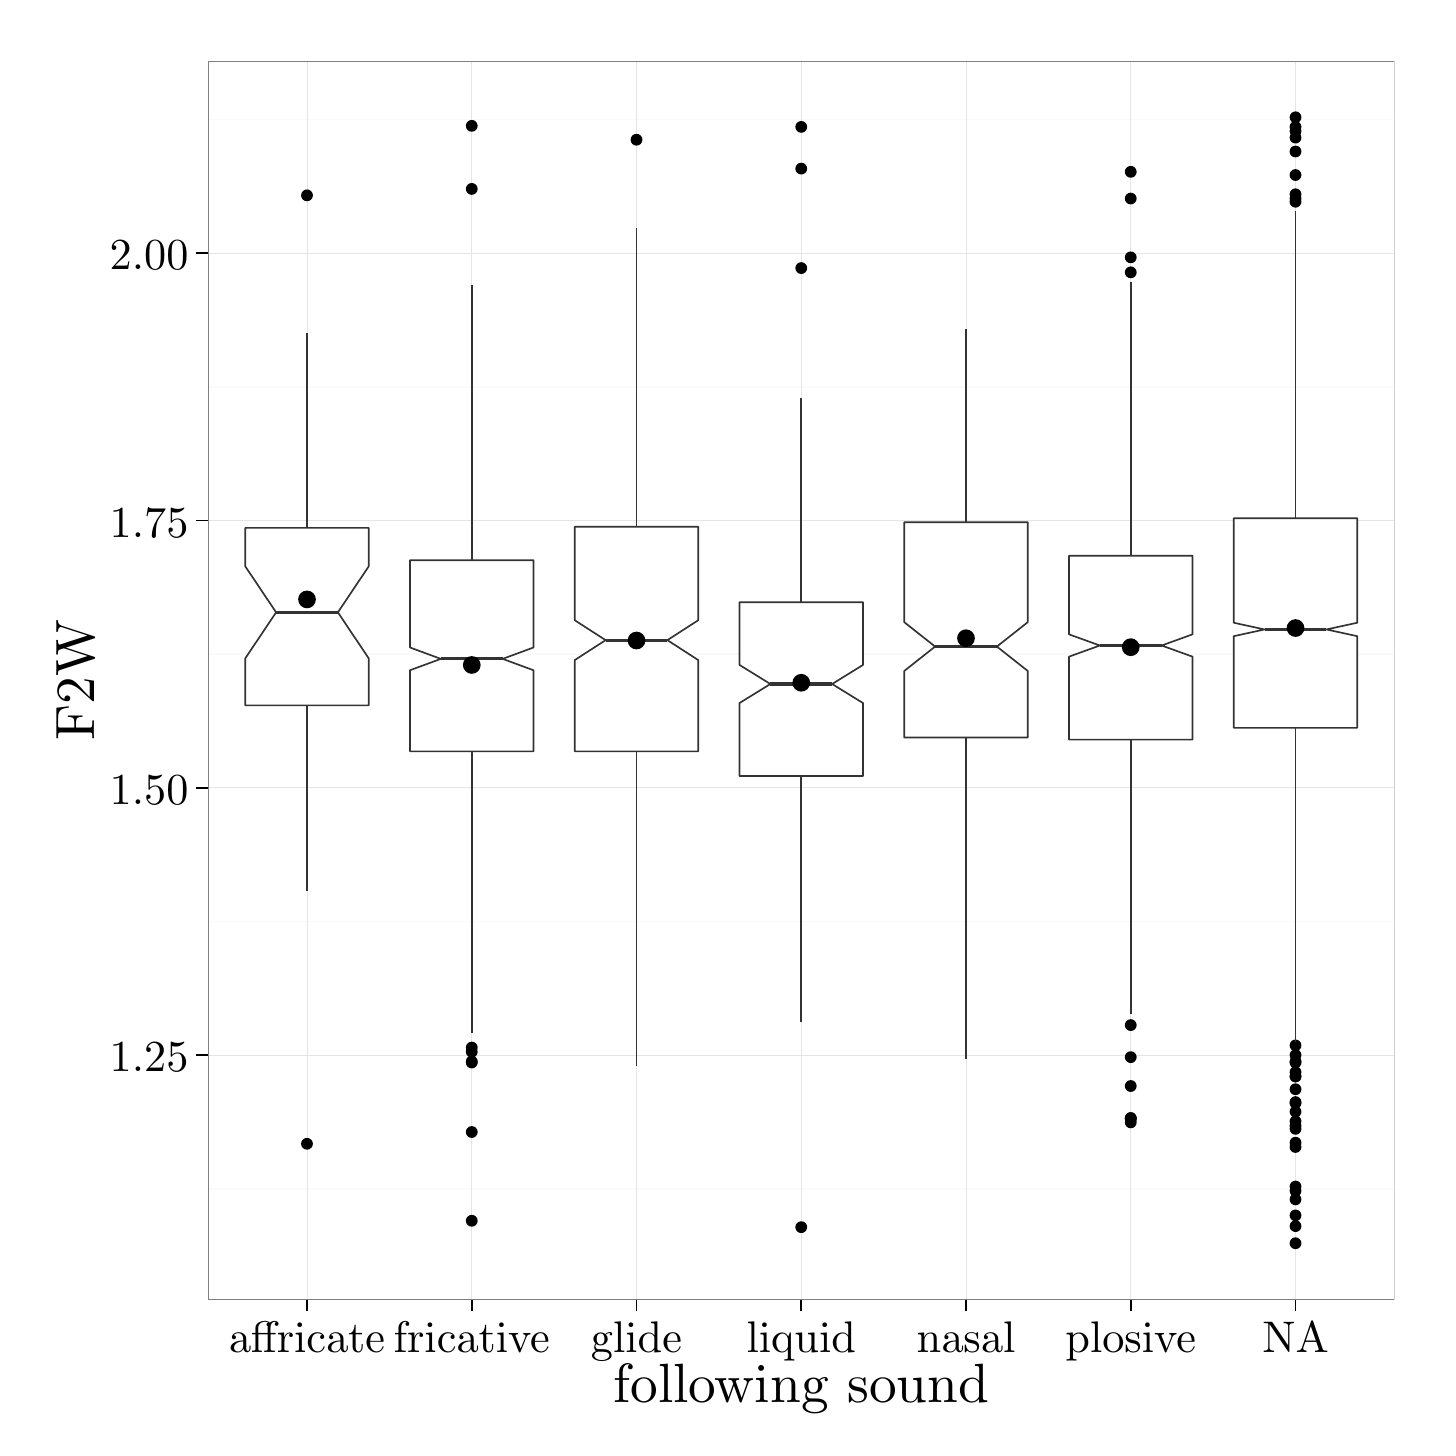
\begin{tikzpicture}[x=1pt,y=1pt]
\definecolor{fillColor}{RGB}{255,255,255}
\path[use as bounding box,fill=fillColor,fill opacity=0.00] (0,0) rectangle (505.89,505.89);
\begin{scope}
\path[clip] (  0.00,  0.00) rectangle (505.89,505.89);
\definecolor{drawColor}{RGB}{255,255,255}
\definecolor{fillColor}{RGB}{255,255,255}

\path[draw=drawColor,line width= 0.6pt,line join=round,line cap=round,fill=fillColor] (  0.00, -0.00) rectangle (505.89,505.89);
\end{scope}
\begin{scope}
\path[clip] ( 65.21, 46.31) rectangle (493.85,493.84);
\definecolor{fillColor}{RGB}{255,255,255}

\path[fill=fillColor] ( 65.21, 46.31) rectangle (493.85,493.84);
\definecolor{drawColor}{gray}{0.98}

\path[draw=drawColor,line width= 0.6pt,line join=round] ( 65.21, 86.36) --
	(493.85, 86.36);

\path[draw=drawColor,line width= 0.6pt,line join=round] ( 65.21,182.95) --
	(493.85,182.95);

\path[draw=drawColor,line width= 0.6pt,line join=round] ( 65.21,279.54) --
	(493.85,279.54);

\path[draw=drawColor,line width= 0.6pt,line join=round] ( 65.21,376.14) --
	(493.85,376.14);

\path[draw=drawColor,line width= 0.6pt,line join=round] ( 65.21,472.73) --
	(493.85,472.73);
\definecolor{drawColor}{gray}{0.90}

\path[draw=drawColor,line width= 0.2pt,line join=round] ( 65.21,134.65) --
	(493.85,134.65);

\path[draw=drawColor,line width= 0.2pt,line join=round] ( 65.21,231.25) --
	(493.85,231.25);

\path[draw=drawColor,line width= 0.2pt,line join=round] ( 65.21,327.84) --
	(493.85,327.84);

\path[draw=drawColor,line width= 0.2pt,line join=round] ( 65.21,424.43) --
	(493.85,424.43);

\path[draw=drawColor,line width= 0.2pt,line join=round] (100.93, 46.31) --
	(100.93,493.84);

\path[draw=drawColor,line width= 0.2pt,line join=round] (160.47, 46.31) --
	(160.47,493.84);

\path[draw=drawColor,line width= 0.2pt,line join=round] (220.00, 46.31) --
	(220.00,493.84);

\path[draw=drawColor,line width= 0.2pt,line join=round] (279.53, 46.31) --
	(279.53,493.84);

\path[draw=drawColor,line width= 0.2pt,line join=round] (339.06, 46.31) --
	(339.06,493.84);

\path[draw=drawColor,line width= 0.2pt,line join=round] (398.59, 46.31) --
	(398.59,493.84);

\path[draw=drawColor,line width= 0.2pt,line join=round] (458.13, 46.31) --
	(458.13,493.84);
\definecolor{fillColor}{RGB}{0,0,0}

\path[fill=fillColor] (100.93,445.30) circle (  2.13);

\path[fill=fillColor] (100.93,102.58) circle (  2.13);
\definecolor{drawColor}{gray}{0.20}

\path[draw=drawColor,line width= 0.6pt,line join=round] (100.93,325.13) -- (100.93,395.45);

\path[draw=drawColor,line width= 0.6pt,line join=round] (100.93,261.00) -- (100.93,193.77);
\definecolor{fillColor}{RGB}{255,255,255}

\path[draw=drawColor,line width= 0.6pt,line join=round,line cap=round,fill=fillColor] ( 78.61,325.13) --
	( 78.61,311.27) --
	( 89.77,294.61) --
	( 78.61,277.95) --
	( 78.61,261.00) --
	(123.26,261.00) --
	(123.26,277.95) --
	(112.10,294.61) --
	(123.26,311.27) --
	(123.26,325.13) --
	( 78.61,325.13) --
	cycle;

\path[draw=drawColor,line width= 1.1pt,line join=round] ( 89.77,294.61) -- (112.10,294.61);
\definecolor{fillColor}{RGB}{0,0,0}

\path[fill=fillColor] (160.47,137.36) circle (  2.13);

\path[fill=fillColor] (160.47,132.33) circle (  2.13);

\path[fill=fillColor] (160.47,106.83) circle (  2.13);

\path[fill=fillColor] (160.47,470.41) circle (  2.13);

\path[fill=fillColor] (160.47,447.62) circle (  2.13);

\path[fill=fillColor] (160.47,135.81) circle (  2.13);

\path[fill=fillColor] (160.47,131.95) circle (  2.13);

\path[fill=fillColor] (160.47, 74.76) circle (  2.13);

\path[draw=drawColor,line width= 0.6pt,line join=round] (160.47,313.45) -- (160.47,412.84);

\path[draw=drawColor,line width= 0.6pt,line join=round] (160.47,244.38) -- (160.47,142.77);
\definecolor{fillColor}{RGB}{255,255,255}

\path[draw=drawColor,line width= 0.6pt,line join=round,line cap=round,fill=fillColor] (138.14,313.45) --
	(138.14,281.92) --
	(149.30,277.80) --
	(138.14,273.69) --
	(138.14,244.38) --
	(182.79,244.38) --
	(182.79,273.69) --
	(171.63,277.80) --
	(182.79,281.92) --
	(182.79,313.45) --
	(138.14,313.45) --
	cycle;

\path[draw=drawColor,line width= 1.1pt,line join=round] (149.30,277.80) -- (171.63,277.80);
\definecolor{fillColor}{RGB}{0,0,0}

\path[fill=fillColor] (220.00,465.39) circle (  2.13);

\path[draw=drawColor,line width= 0.6pt,line join=round] (220.00,325.52) -- (220.00,433.32);

\path[draw=drawColor,line width= 0.6pt,line join=round] (220.00,244.38) -- (220.00,130.79);
\definecolor{fillColor}{RGB}{255,255,255}

\path[draw=drawColor,line width= 0.6pt,line join=round,line cap=round,fill=fillColor] (197.67,325.52) --
	(197.67,291.77) --
	(208.84,284.57) --
	(197.67,277.36) --
	(197.67,244.38) --
	(242.32,244.38) --
	(242.32,277.36) --
	(231.16,284.57) --
	(242.32,291.77) --
	(242.32,325.52) --
	(197.67,325.52) --
	cycle;

\path[draw=drawColor,line width= 1.1pt,line join=round] (208.84,284.57) -- (231.16,284.57);
\definecolor{fillColor}{RGB}{0,0,0}

\path[fill=fillColor] (279.53,454.96) circle (  2.13);

\path[fill=fillColor] (279.53,470.03) circle (  2.13);

\path[fill=fillColor] (279.53, 72.45) circle (  2.13);

\path[fill=fillColor] (279.53,419.02) circle (  2.13);

\path[draw=drawColor,line width= 0.6pt,line join=round] (279.53,298.28) -- (279.53,371.89);

\path[draw=drawColor,line width= 0.6pt,line join=round] (279.53,235.50) -- (279.53,146.63);
\definecolor{fillColor}{RGB}{255,255,255}

\path[draw=drawColor,line width= 0.6pt,line join=round,line cap=round,fill=fillColor] (257.20,298.28) --
	(257.20,275.62) --
	(268.37,268.72) --
	(257.20,261.83) --
	(257.20,235.50) --
	(301.85,235.50) --
	(301.85,261.83) --
	(290.69,268.72) --
	(301.85,275.62) --
	(301.85,298.28) --
	(257.20,298.28) --
	cycle;

\path[draw=drawColor,line width= 1.1pt,line join=round] (268.37,268.72) -- (290.69,268.72);

\path[draw=drawColor,line width= 0.6pt,line join=round] (339.06,327.16) -- (339.06,397.00);

\path[draw=drawColor,line width= 0.6pt,line join=round] (339.06,249.41) -- (339.06,133.11);

\path[draw=drawColor,line width= 0.6pt,line join=round,line cap=round,fill=fillColor] (316.74,327.16) --
	(316.74,291.07) --
	(327.90,282.25) --
	(316.74,273.43) --
	(316.74,249.41) --
	(361.39,249.41) --
	(361.39,273.43) --
	(350.22,282.25) --
	(361.39,291.07) --
	(361.39,327.16) --
	(316.74,327.16) --
	cycle;

\path[draw=drawColor,line width= 1.1pt,line join=round] (327.90,282.25) -- (350.22,282.25);
\definecolor{fillColor}{RGB}{0,0,0}

\path[fill=fillColor] (398.59,111.86) circle (  2.13);

\path[fill=fillColor] (398.59,110.31) circle (  2.13);

\path[fill=fillColor] (398.59,453.80) circle (  2.13);

\path[fill=fillColor] (398.59,145.47) circle (  2.13);

\path[fill=fillColor] (398.59,133.88) circle (  2.13);

\path[fill=fillColor] (398.59,417.48) circle (  2.13);

\path[fill=fillColor] (398.59,444.14) circle (  2.13);

\path[fill=fillColor] (398.59,422.89) circle (  2.13);

\path[fill=fillColor] (398.59,111.47) circle (  2.13);

\path[fill=fillColor] (398.59,111.86) circle (  2.13);

\path[fill=fillColor] (398.59,123.45) circle (  2.13);

\path[draw=drawColor,line width= 0.6pt,line join=round] (398.59,315.09) -- (398.59,414.00);

\path[draw=drawColor,line width= 0.6pt,line join=round] (398.59,248.63) -- (398.59,149.33);
\definecolor{fillColor}{RGB}{255,255,255}

\path[draw=drawColor,line width= 0.6pt,line join=round,line cap=round,fill=fillColor] (376.27,315.09) --
	(376.27,286.67) --
	(387.43,282.63) --
	(376.27,278.60) --
	(376.27,248.63) --
	(420.92,248.63) --
	(420.92,278.60) --
	(409.76,282.63) --
	(420.92,286.67) --
	(420.92,315.09) --
	(376.27,315.09) --
	cycle;

\path[draw=drawColor,line width= 1.1pt,line join=round] (387.43,282.63) -- (409.76,282.63);
\definecolor{fillColor}{RGB}{0,0,0}

\path[fill=fillColor] (458.13,132.33) circle (  2.13);

\path[fill=fillColor] (458.13,126.92) circle (  2.13);

\path[fill=fillColor] (458.13,114.17) circle (  2.13);

\path[fill=fillColor] (458.13,128.47) circle (  2.13);

\path[fill=fillColor] (458.13,107.99) circle (  2.13);

\path[fill=fillColor] (458.13,442.98) circle (  2.13);

\path[fill=fillColor] (458.13,445.68) circle (  2.13);

\path[fill=fillColor] (458.13,468.48) circle (  2.13);

\path[fill=fillColor] (458.13,452.64) circle (  2.13);

\path[fill=fillColor] (458.13, 85.58) circle (  2.13);

\path[fill=fillColor] (458.13,444.14) circle (  2.13);

\path[fill=fillColor] (458.13,470.03) circle (  2.13);

\path[fill=fillColor] (458.13,466.16) circle (  2.13);

\path[fill=fillColor] (458.13,110.70) circle (  2.13);

\path[fill=fillColor] (458.13,117.27) circle (  2.13);

\path[fill=fillColor] (458.13,102.97) circle (  2.13);

\path[fill=fillColor] (458.13, 72.83) circle (  2.13);

\path[fill=fillColor] (458.13,473.50) circle (  2.13);

\path[fill=fillColor] (458.13, 82.49) circle (  2.13);

\path[fill=fillColor] (458.13,101.42) circle (  2.13);

\path[fill=fillColor] (458.13,138.13) circle (  2.13);

\path[fill=fillColor] (458.13, 66.65) circle (  2.13);

\path[fill=fillColor] (458.13,131.95) circle (  2.13);

\path[fill=fillColor] (458.13, 76.70) circle (  2.13);

\path[fill=fillColor] (458.13,461.14) circle (  2.13);

\path[fill=fillColor] (458.13,126.92) circle (  2.13);

\path[fill=fillColor] (458.13,109.15) circle (  2.13);

\path[fill=fillColor] (458.13,117.65) circle (  2.13);

\path[fill=fillColor] (458.13,134.65) circle (  2.13);

\path[fill=fillColor] (458.13,122.29) circle (  2.13);

\path[fill=fillColor] (458.13, 87.13) circle (  2.13);

\path[draw=drawColor,line width= 0.6pt,line join=round] (458.13,328.61) -- (458.13,439.50);

\path[draw=drawColor,line width= 0.6pt,line join=round] (458.13,252.88) -- (458.13,139.29);
\definecolor{fillColor}{RGB}{255,255,255}

\path[draw=drawColor,line width= 0.6pt,line join=round,line cap=round,fill=fillColor] (435.80,328.61) --
	(435.80,290.86) --
	(446.96,288.43) --
	(435.80,286.00) --
	(435.80,252.88) --
	(480.45,252.88) --
	(480.45,286.00) --
	(469.29,288.43) --
	(480.45,290.86) --
	(480.45,328.61) --
	(435.80,328.61) --
	cycle;

\path[draw=drawColor,line width= 1.1pt,line join=round] (446.96,288.43) -- (469.29,288.43);
\definecolor{fillColor}{RGB}{0,0,0}

\path[fill=fillColor] (100.93,299.29) circle (  3.20);

\path[fill=fillColor] (160.47,275.60) circle (  3.20);

\path[fill=fillColor] (220.00,284.44) circle (  3.20);

\path[fill=fillColor] (279.53,269.16) circle (  3.20);

\path[fill=fillColor] (339.06,285.27) circle (  3.20);

\path[fill=fillColor] (398.59,282.02) circle (  3.20);

\path[fill=fillColor] (458.13,288.94) circle (  3.20);
\definecolor{drawColor}{gray}{0.50}

\path[draw=drawColor,line width= 0.6pt,line join=round,line cap=round] ( 65.21, 46.31) rectangle (493.85,493.84);
\end{scope}
\begin{scope}
\path[clip] (  0.00,  0.00) rectangle (505.89,505.89);
\definecolor{drawColor}{RGB}{0,0,0}

\node[text=drawColor,anchor=base east,inner sep=0pt, outer sep=0pt, scale=  1.60] at ( 58.10,128.62) {1.25};

\node[text=drawColor,anchor=base east,inner sep=0pt, outer sep=0pt, scale=  1.60] at ( 58.10,225.21) {1.50};

\node[text=drawColor,anchor=base east,inner sep=0pt, outer sep=0pt, scale=  1.60] at ( 58.10,321.81) {1.75};

\node[text=drawColor,anchor=base east,inner sep=0pt, outer sep=0pt, scale=  1.60] at ( 58.10,418.40) {2.00};
\end{scope}
\begin{scope}
\path[clip] (  0.00,  0.00) rectangle (505.89,505.89);
\definecolor{drawColor}{RGB}{0,0,0}

\path[draw=drawColor,line width= 0.6pt,line join=round] ( 60.95,134.65) --
	( 65.21,134.65);

\path[draw=drawColor,line width= 0.6pt,line join=round] ( 60.95,231.25) --
	( 65.21,231.25);

\path[draw=drawColor,line width= 0.6pt,line join=round] ( 60.95,327.84) --
	( 65.21,327.84);

\path[draw=drawColor,line width= 0.6pt,line join=round] ( 60.95,424.43) --
	( 65.21,424.43);
\end{scope}
\begin{scope}
\path[clip] (  0.00,  0.00) rectangle (505.89,505.89);
\definecolor{drawColor}{RGB}{0,0,0}

\path[draw=drawColor,line width= 0.6pt,line join=round] (100.93, 42.04) --
	(100.93, 46.31);

\path[draw=drawColor,line width= 0.6pt,line join=round] (160.47, 42.04) --
	(160.47, 46.31);

\path[draw=drawColor,line width= 0.6pt,line join=round] (220.00, 42.04) --
	(220.00, 46.31);

\path[draw=drawColor,line width= 0.6pt,line join=round] (279.53, 42.04) --
	(279.53, 46.31);

\path[draw=drawColor,line width= 0.6pt,line join=round] (339.06, 42.04) --
	(339.06, 46.31);

\path[draw=drawColor,line width= 0.6pt,line join=round] (398.59, 42.04) --
	(398.59, 46.31);

\path[draw=drawColor,line width= 0.6pt,line join=round] (458.13, 42.04) --
	(458.13, 46.31);
\end{scope}
\begin{scope}
\path[clip] (  0.00,  0.00) rectangle (505.89,505.89);
\definecolor{drawColor}{RGB}{0,0,0}

\node[text=drawColor,anchor=base,inner sep=0pt, outer sep=0pt, scale=  1.60] at (100.93, 27.13) {affricate};

\node[text=drawColor,anchor=base,inner sep=0pt, outer sep=0pt, scale=  1.60] at (160.47, 27.13) {fricative};

\node[text=drawColor,anchor=base,inner sep=0pt, outer sep=0pt, scale=  1.60] at (220.00, 27.13) {glide};

\node[text=drawColor,anchor=base,inner sep=0pt, outer sep=0pt, scale=  1.60] at (279.53, 27.13) {liquid};

\node[text=drawColor,anchor=base,inner sep=0pt, outer sep=0pt, scale=  1.60] at (339.06, 27.13) {nasal};

\node[text=drawColor,anchor=base,inner sep=0pt, outer sep=0pt, scale=  1.60] at (398.59, 27.13) {plosive};

\node[text=drawColor,anchor=base,inner sep=0pt, outer sep=0pt, scale=  1.60] at (458.13, 27.13) {NA};
\end{scope}
\begin{scope}
\path[clip] (  0.00,  0.00) rectangle (505.89,505.89);
\definecolor{drawColor}{RGB}{0,0,0}

\node[text=drawColor,anchor=base,inner sep=0pt, outer sep=0pt, scale=  2.00] at (279.53,  9.03) {following sound};
\end{scope}
\begin{scope}
\path[clip] (  0.00,  0.00) rectangle (505.89,505.89);
\definecolor{drawColor}{RGB}{0,0,0}

\node[text=drawColor,rotate= 90.00,anchor=base,inner sep=0pt, outer sep=0pt, scale=  2.00] at ( 24.12,270.08) {F2W};
\end{scope}
\end{tikzpicture}
} 
		\caption{following sound}
		\label{fig.box.f2w.happy.follsound}
	\end{subfigure}
	\caption{happ\textsc{y} (F2) by preceding and following sound}
\end{figure}

Figure \ref{fig.box.f2w.happy.presound} is a box plot of F2 values (on the y-axis) sorted by preceding (manner of) consonant (on the x-axis).
``NA'' here stands for observations where no phonemic transcription was available for the carrier word and which, as a consequence, could not be coded for preceding sound (this mostly concerned proper names, 81 observations in total).
Judging from this graph, it seems as if happ\textsc{y} measurements following liquids were the odd ones out (with lower values of F2, on average), as the remaining means are much more similar to each other and the confidence intervals of the medians (illustrated by the notches) frequently overlap.
Cases where happ\textsc{y} is preceded by a liquid were also the ones (along with, to a lesser extent, preceding fricatives) that were found to be significantly different by the mixed linear effects regression model.
It should be noted that this context (preceding liquid) includes regularly formed adverbs, and therefore, by itself, accounts for the majority of happ\textsc{y} observations (2790 out of 4565, or 61.12\%), which means that the statistical basis for this phonological environment\is{phonological context} is considerably larger than for the others.
Furthermore, high \isi{frequency} words such as \emph{very} or \emph{really} are to be found in this category, so it is not unlikely that \isi{phonological context} is here mixed up with other features such as duration (see below).

Interestingly, a \emph{following} liquid (at the beginning of the next word) seems to have a very similar effect on F2 measures as a preceding one (lowering of F2 in this context has been attested before, cf. \citealt[26]{lehiste1964}).
The corresponding box plot for F2 by following phoneme (Figure \ref{fig.box.f2w.happy.follsound}) shows happ\textsc{y} to be somewhat more central (lower F2) when a liquid follows.
This is in line with the regression model (which found a negative correlation coefficient for this context).
The significantly negative coefficient (in the model) for a following fricative is less obvious in this figure: while mean and median are somewhat lower, they do not appear to be significantly so (cf., for instance, the partially overlapping confidence notches of ``fricative'' and the neighbouring ``glide'').
The same holds for happ\textsc{y} observations that are followed by an affricate.
The mean in this category is higher than for other following consonants (corresponds to the positive coefficient found in the regression), but there seems to be a lot of noise in the raw data, which results in quite a large confidence interval (see the notches of the ``affricate'' box).

\begin{figure}[h!]
	\centering
		\definecolor{shadecolor}{rgb}{0.969, 0.969, 0.969}
		\resizebox{0.5\linewidth}{!}{% Created by tikzDevice version 0.8.1 on 2016-02-09 02:13:49
% !TEX encoding = UTF-8 Unicode
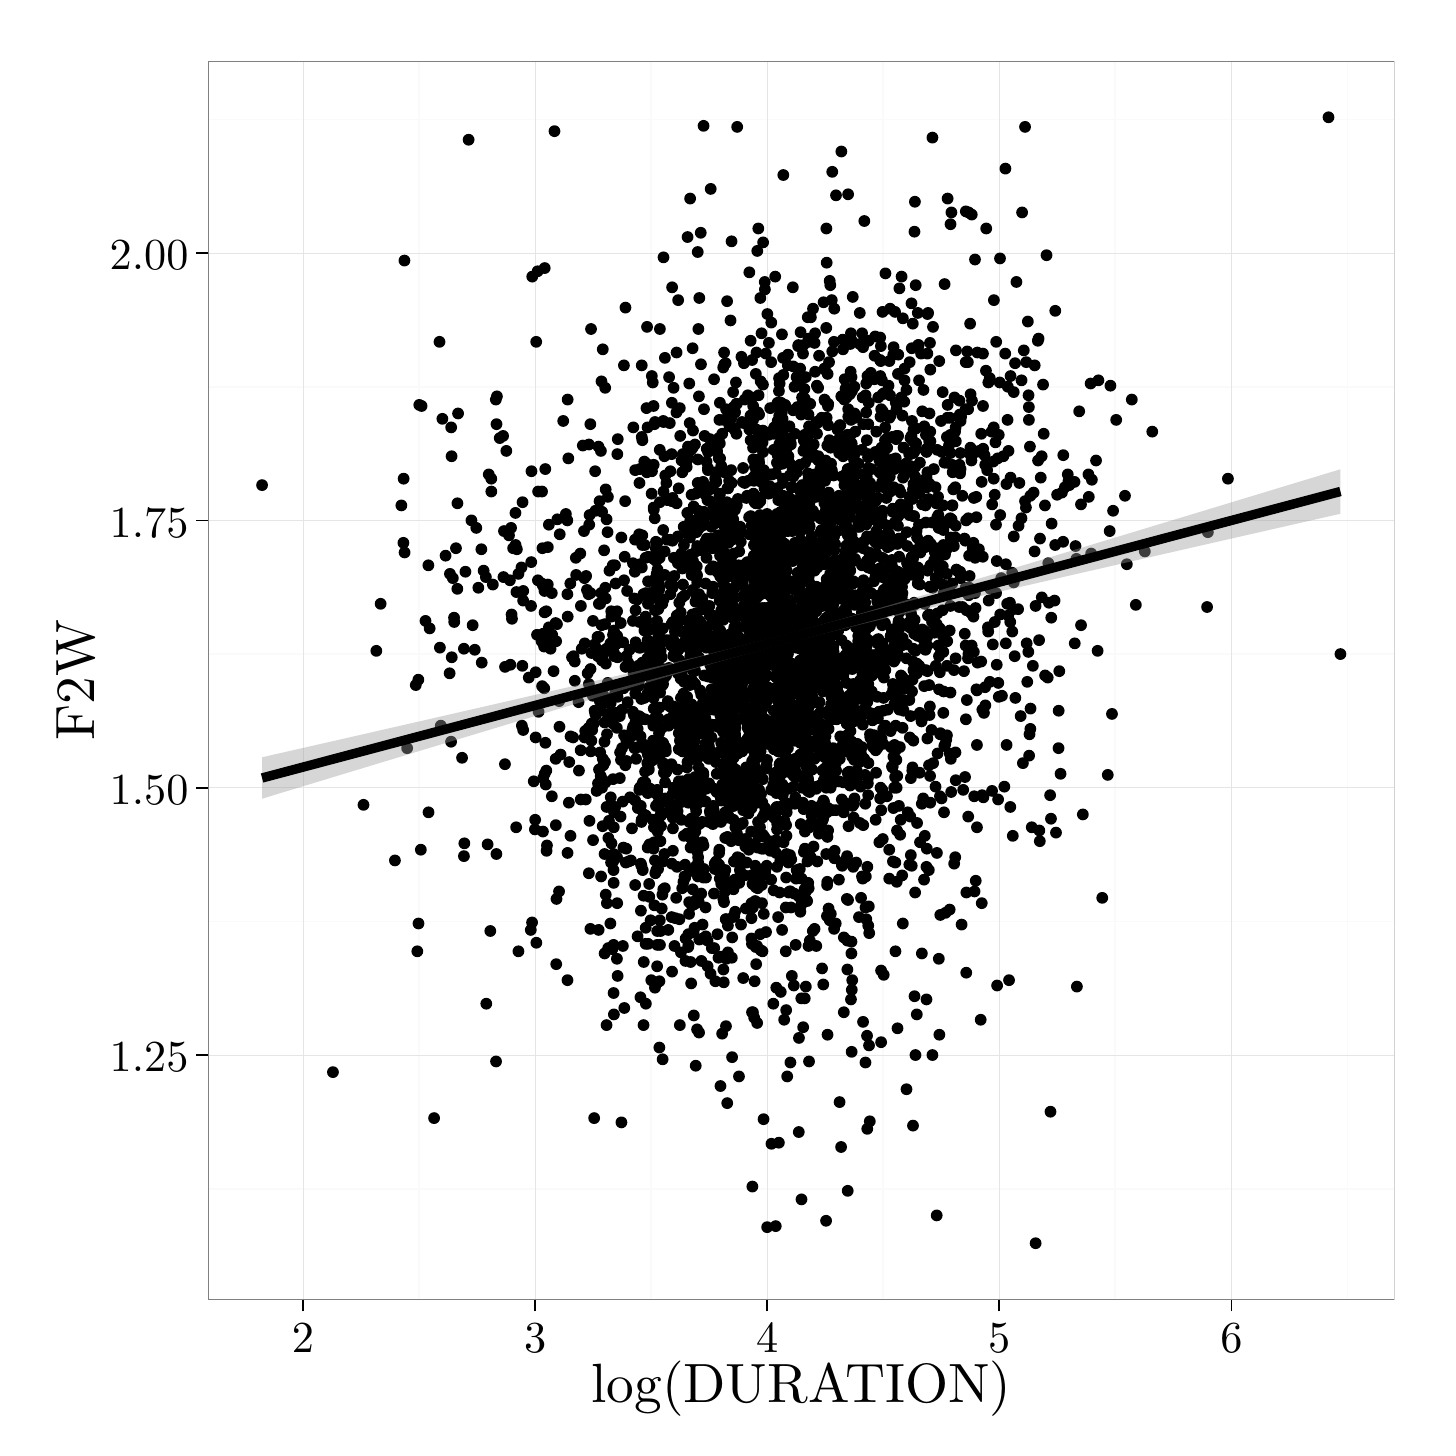
\begin{tikzpicture}[x=1pt,y=1pt]
\definecolor{fillColor}{RGB}{255,255,255}
\path[use as bounding box,fill=fillColor,fill opacity=0.00] (0,0) rectangle (505.89,505.89);
\begin{scope}
\path[clip] (  0.00,  0.00) rectangle (505.89,505.89);
\definecolor{drawColor}{RGB}{255,255,255}
\definecolor{fillColor}{RGB}{255,255,255}

\path[draw=drawColor,line width= 0.6pt,line join=round,line cap=round,fill=fillColor] (  0.00, -0.00) rectangle (505.89,505.89);
\end{scope}
\begin{scope}
\path[clip] ( 65.21, 46.31) rectangle (493.85,493.84);
\definecolor{fillColor}{RGB}{255,255,255}

\path[fill=fillColor] ( 65.21, 46.31) rectangle (493.85,493.84);
\definecolor{drawColor}{gray}{0.98}

\path[draw=drawColor,line width= 0.6pt,line join=round] ( 65.21, 86.36) --
	(493.85, 86.36);

\path[draw=drawColor,line width= 0.6pt,line join=round] ( 65.21,182.95) --
	(493.85,182.95);

\path[draw=drawColor,line width= 0.6pt,line join=round] ( 65.21,279.54) --
	(493.85,279.54);

\path[draw=drawColor,line width= 0.6pt,line join=round] ( 65.21,376.14) --
	(493.85,376.14);

\path[draw=drawColor,line width= 0.6pt,line join=round] ( 65.21,472.73) --
	(493.85,472.73);

\path[draw=drawColor,line width= 0.6pt,line join=round] (141.42, 46.31) --
	(141.42,493.84);

\path[draw=drawColor,line width= 0.6pt,line join=round] (225.28, 46.31) --
	(225.28,493.84);

\path[draw=drawColor,line width= 0.6pt,line join=round] (309.14, 46.31) --
	(309.14,493.84);

\path[draw=drawColor,line width= 0.6pt,line join=round] (393.01, 46.31) --
	(393.01,493.84);

\path[draw=drawColor,line width= 0.6pt,line join=round] (476.87, 46.31) --
	(476.87,493.84);
\definecolor{drawColor}{gray}{0.90}

\path[draw=drawColor,line width= 0.2pt,line join=round] ( 65.21,134.65) --
	(493.85,134.65);

\path[draw=drawColor,line width= 0.2pt,line join=round] ( 65.21,231.25) --
	(493.85,231.25);

\path[draw=drawColor,line width= 0.2pt,line join=round] ( 65.21,327.84) --
	(493.85,327.84);

\path[draw=drawColor,line width= 0.2pt,line join=round] ( 65.21,424.43) --
	(493.85,424.43);

\path[draw=drawColor,line width= 0.2pt,line join=round] ( 99.48, 46.31) --
	( 99.48,493.84);

\path[draw=drawColor,line width= 0.2pt,line join=round] (183.35, 46.31) --
	(183.35,493.84);

\path[draw=drawColor,line width= 0.2pt,line join=round] (267.21, 46.31) --
	(267.21,493.84);

\path[draw=drawColor,line width= 0.2pt,line join=round] (351.07, 46.31) --
	(351.07,493.84);

\path[draw=drawColor,line width= 0.2pt,line join=round] (434.94, 46.31) --
	(434.94,493.84);
\definecolor{fillColor}{RGB}{0,0,0}

\path[fill=fillColor] (270.43,298.47) circle (  2.13);

\path[fill=fillColor] (247.21,254.04) circle (  2.13);

\path[fill=fillColor] (313.90,241.29) circle (  2.13);

\path[fill=fillColor] (253.33,255.97) circle (  2.13);

\path[fill=fillColor] (263.10,334.02) circle (  2.13);

\path[fill=fillColor] (263.30,360.68) circle (  2.13);

\path[fill=fillColor] (297.12,244.00) circle (  2.13);

\path[fill=fillColor] (278.97,247.86) circle (  2.13);

\path[fill=fillColor] (195.00,327.84) circle (  2.13);

\path[fill=fillColor] (221.25,312.00) circle (  2.13);

\path[fill=fillColor] (282.67,286.88) circle (  2.13);

\path[fill=fillColor] (271.32,300.41) circle (  2.13);

\path[fill=fillColor] (251.39,165.56) circle (  2.13);

\path[fill=fillColor] (274.28,304.27) circle (  2.13);

\path[fill=fillColor] (262.14,248.25) circle (  2.13);

\path[fill=fillColor] (186.27,234.72) circle (  2.13);

\path[fill=fillColor] (225.34,161.70) circle (  2.13);

\path[fill=fillColor] (204.21,264.47) circle (  2.13);

\path[fill=fillColor] (257.58,267.18) circle (  2.13);

\path[fill=fillColor] (333.51,321.66) circle (  2.13);

\path[fill=fillColor] (253.99,255.97) circle (  2.13);

\path[fill=fillColor] (292.64,360.68) circle (  2.13);

\path[fill=fillColor] (245.70,166.72) circle (  2.13);

\path[fill=fillColor] (235.40,293.84) circle (  2.13);

\path[fill=fillColor] (246.47,339.04) circle (  2.13);

\path[fill=fillColor] (366.90,376.91) circle (  2.13);

\path[fill=fillColor] (252.43,267.95) circle (  2.13);

\path[fill=fillColor] (208.48,171.36) circle (  2.13);

\path[fill=fillColor] (268.76,318.18) circle (  2.13);

\path[fill=fillColor] (254.32,300.79) circle (  2.13);

\path[fill=fillColor] (284.24,343.68) circle (  2.13);

\path[fill=fillColor] (271.62,325.52) circle (  2.13);

\path[fill=fillColor] (273.66,312.00) circle (  2.13);

\path[fill=fillColor] (224.18,305.82) circle (  2.13);

\path[fill=fillColor] (248.02,378.84) circle (  2.13);

\path[fill=fillColor] (303.79,240.13) circle (  2.13);

\path[fill=fillColor] (267.14,221.59) circle (  2.13);

\path[fill=fillColor] (245.17,281.86) circle (  2.13);

\path[fill=fillColor] (286.12,262.16) circle (  2.13);

\path[fill=fillColor] (325.77,293.84) circle (  2.13);

\path[fill=fillColor] (281.77,204.59) circle (  2.13);

\path[fill=fillColor] (310.34,306.59) circle (  2.13);

\path[fill=fillColor] (261.91,288.82) circle (  2.13);

\path[fill=fillColor] (283.71,179.47) circle (  2.13);

\path[fill=fillColor] (279.15,247.47) circle (  2.13);

\path[fill=fillColor] (257.35,199.18) circle (  2.13);

\path[fill=fillColor] (247.03,266.79) circle (  2.13);

\path[fill=fillColor] (281.89,242.06) circle (  2.13);

\path[fill=fillColor] (232.63,290.36) circle (  2.13);

\path[fill=fillColor] (271.64,306.59) circle (  2.13);

\path[fill=fillColor] (256.16,255.97) circle (  2.13);

\path[fill=fillColor] (255.01,322.43) circle (  2.13);

\path[fill=fillColor] (256.86,212.31) circle (  2.13);

\path[fill=fillColor] (268.17,300.79) circle (  2.13);

\path[fill=fillColor] (291.54,273.75) circle (  2.13);

\path[fill=fillColor] (229.71,272.97) circle (  2.13);

\path[fill=fillColor] (184.38,306.20) circle (  2.13);

\path[fill=fillColor] (265.18,395.45) circle (  2.13);

\path[fill=fillColor] (218.36,216.56) circle (  2.13);

\path[fill=fillColor] (293.15,336.73) circle (  2.13);

\path[fill=fillColor] (252.77,322.43) circle (  2.13);

\path[fill=fillColor] (269.63,320.88) circle (  2.13);

\path[fill=fillColor] (289.21,345.61) circle (  2.13);

\path[fill=fillColor] (247.57,292.68) circle (  2.13);

\path[fill=fillColor] (252.24,313.54) circle (  2.13);

\path[fill=fillColor] (249.73,350.25) circle (  2.13);

\path[fill=fillColor] (296.19,313.93) circle (  2.13);

\path[fill=fillColor] (302.52,269.11) circle (  2.13);

\path[fill=fillColor] (279.85,340.59) circle (  2.13);

\path[fill=fillColor] (274.27,309.68) circle (  2.13);

\path[fill=fillColor] (258.73,363.00) circle (  2.13);

\path[fill=fillColor] (294.10,276.07) circle (  2.13);

\path[fill=fillColor] (262.85,348.70) circle (  2.13);

\path[fill=fillColor] (251.34,261.00) circle (  2.13);

\path[fill=fillColor] (248.55,345.23) circle (  2.13);

\path[fill=fillColor] (229.64,324.36) circle (  2.13);

\path[fill=fillColor] (253.97,234.72) circle (  2.13);

\path[fill=fillColor] (271.06,264.86) circle (  2.13);

\path[fill=fillColor] (255.15,296.54) circle (  2.13);

\path[fill=fillColor] (239.92,308.13) circle (  2.13);

\path[fill=fillColor] (284.89,336.34) circle (  2.13);

\path[fill=fillColor] (195.36,350.25) circle (  2.13);

\path[fill=fillColor] (270.89,321.27) circle (  2.13);

\path[fill=fillColor] (282.43,256.75) circle (  2.13);

\path[fill=fillColor] (270.84,218.11) circle (  2.13);

\path[fill=fillColor] (250.09,198.40) circle (  2.13);

\path[fill=fillColor] (186.76,302.34) circle (  2.13);

\path[fill=fillColor] (223.73,345.23) circle (  2.13);

\path[fill=fillColor] (222.12,356.82) circle (  2.13);

\path[fill=fillColor] (250.15,271.81) circle (  2.13);

\path[fill=fillColor] (250.24,257.52) circle (  2.13);

\path[fill=fillColor] (187.41,295.00) circle (  2.13);

\path[fill=fillColor] (235.18,281.09) circle (  2.13);

\path[fill=fillColor] (306.39,291.91) circle (  2.13);

\path[fill=fillColor] (262.58,267.95) circle (  2.13);

\path[fill=fillColor] (264.05,242.84) circle (  2.13);

\path[fill=fillColor] (248.06,285.72) circle (  2.13);

\path[fill=fillColor] (315.43,260.61) circle (  2.13);

\path[fill=fillColor] (243.05,317.79) circle (  2.13);

\path[fill=fillColor] (242.34,331.32) circle (  2.13);

\path[fill=fillColor] (216.61,302.34) circle (  2.13);

\path[fill=fillColor] (192.16,253.27) circle (  2.13);

\path[fill=fillColor] (224.27,238.59) circle (  2.13);

\path[fill=fillColor] (219.53,226.61) circle (  2.13);

\path[fill=fillColor] (239.05,281.47) circle (  2.13);

\path[fill=fillColor] (247.33,291.13) circle (  2.13);

\path[fill=fillColor] (250.41,227.77) circle (  2.13);

\path[fill=fillColor] (336.55,296.54) circle (  2.13);

\path[fill=fillColor] (249.34,253.27) circle (  2.13);

\path[fill=fillColor] (246.50,222.75) circle (  2.13);

\path[fill=fillColor] (243.18,254.04) circle (  2.13);

\path[fill=fillColor] (277.32,241.68) circle (  2.13);

\path[fill=fillColor] (319.75,270.27) circle (  2.13);

\path[fill=fillColor] (276.79,332.09) circle (  2.13);

\path[fill=fillColor] (301.14,191.45) circle (  2.13);

\path[fill=fillColor] (259.10,260.22) circle (  2.13);

\path[fill=fillColor] (261.93,235.11) circle (  2.13);

\path[fill=fillColor] (252.68,334.41) circle (  2.13);

\path[fill=fillColor] (300.98,328.61) circle (  2.13);

\path[fill=fillColor] (248.24,284.18) circle (  2.13);

\path[fill=fillColor] (273.88,311.23) circle (  2.13);

\path[fill=fillColor] (256.26,369.95) circle (  2.13);

\path[fill=fillColor] (235.80,358.36) circle (  2.13);

\path[fill=fillColor] (240.74,278.38) circle (  2.13);

\path[fill=fillColor] (216.03,274.91) circle (  2.13);

\path[fill=fillColor] (297.48,352.95) circle (  2.13);

\path[fill=fillColor] (268.44,325.91) circle (  2.13);

\path[fill=fillColor] (302.57,235.88) circle (  2.13);

\path[fill=fillColor] (331.23,246.31) circle (  2.13);

\path[fill=fillColor] (274.94,333.25) circle (  2.13);

\path[fill=fillColor] (296.38,322.43) circle (  2.13);

\path[fill=fillColor] (316.50,259.06) circle (  2.13);

\path[fill=fillColor] (253.59,310.07) circle (  2.13);

\path[fill=fillColor] (274.98,251.72) circle (  2.13);

\path[fill=fillColor] (265.51,322.43) circle (  2.13);

\path[fill=fillColor] (304.49,249.41) circle (  2.13);

\path[fill=fillColor] (280.28,271.81) circle (  2.13);

\path[fill=fillColor] (236.06,171.74) circle (  2.13);

\path[fill=fillColor] (266.46,285.34) circle (  2.13);

\path[fill=fillColor] (239.06,218.88) circle (  2.13);

\path[fill=fillColor] (288.10,287.66) circle (  2.13);

\path[fill=fillColor] (269.92,234.72) circle (  2.13);

\path[fill=fillColor] (242.12,341.36) circle (  2.13);

\path[fill=fillColor] (274.69,383.86) circle (  2.13);

\path[fill=fillColor] (267.84,288.04) circle (  2.13);

\path[fill=fillColor] (261.91,235.50) circle (  2.13);

\path[fill=fillColor] (247.02,325.52) circle (  2.13);

\path[fill=fillColor] (246.71,310.07) circle (  2.13);

\path[fill=fillColor] (268.07,275.68) circle (  2.13);

\path[fill=fillColor] (225.28,270.66) circle (  2.13);

\path[fill=fillColor] (281.78,289.97) circle (  2.13);

\path[fill=fillColor] (345.13,314.70) circle (  2.13);

\path[fill=fillColor] (337.10,346.39) circle (  2.13);

\path[fill=fillColor] (267.24,271.81) circle (  2.13);

\path[fill=fillColor] (250.06,287.66) circle (  2.13);

\path[fill=fillColor] (287.48,337.11) circle (  2.13);

\path[fill=fillColor] (288.84,243.22) circle (  2.13);

\path[fill=fillColor] (240.61,213.09) circle (  2.13);

\path[fill=fillColor] (261.69,275.68) circle (  2.13);

\path[fill=fillColor] (239.76,288.43) circle (  2.13);

\path[fill=fillColor] (157.79,211.15) circle (  2.13);

\path[fill=fillColor] (285.90,261.77) circle (  2.13);

\path[fill=fillColor] (263.04,271.81) circle (  2.13);

\path[fill=fillColor] (254.93,285.34) circle (  2.13);

\path[fill=fillColor] (307.74,279.93) circle (  2.13);

\path[fill=fillColor] (264.19,296.16) circle (  2.13);

\path[fill=fillColor] (190.96,284.18) circle (  2.13);

\path[fill=fillColor] (270.59,271.04) circle (  2.13);

\path[fill=fillColor] (253.46,342.14) circle (  2.13);

\path[fill=fillColor] (314.90,314.70) circle (  2.13);

\path[fill=fillColor] (278.13,335.18) circle (  2.13);

\path[fill=fillColor] (295.33,325.91) circle (  2.13);

\path[fill=fillColor] (263.93,268.72) circle (  2.13);

\path[fill=fillColor] (251.39,300.02) circle (  2.13);

\path[fill=fillColor] (224.01,361.45) circle (  2.13);

\path[fill=fillColor] (230.23,194.93) circle (  2.13);

\path[fill=fillColor] (222.31,233.18) circle (  2.13);

\path[fill=fillColor] (226.25,331.70) circle (  2.13);

\path[fill=fillColor] (263.75,263.31) circle (  2.13);

\path[fill=fillColor] (279.19,308.13) circle (  2.13);

\path[fill=fillColor] (275.25,264.86) circle (  2.13);

\path[fill=fillColor] (227.52,306.20) circle (  2.13);

\path[fill=fillColor] (241.83,294.22) circle (  2.13);

\path[fill=fillColor] (284.71,218.11) circle (  2.13);

\path[fill=fillColor] (274.61,329.38) circle (  2.13);

\path[fill=fillColor] (321.33,272.59) circle (  2.13);

\path[fill=fillColor] (202.73,252.88) circle (  2.13);

\path[fill=fillColor] (256.12,286.88) circle (  2.13);

\path[fill=fillColor] (228.28,161.31) circle (  2.13);

\path[fill=fillColor] (239.19,289.59) circle (  2.13);

\path[fill=fillColor] (258.45,341.75) circle (  2.13);

\path[fill=fillColor] (279.63,339.04) circle (  2.13);

\path[fill=fillColor] (235.28,245.16) circle (  2.13);

\path[fill=fillColor] (207.99,239.36) circle (  2.13);

\path[fill=fillColor] (257.79,284.95) circle (  2.13);

\path[fill=fillColor] (248.08,173.29) circle (  2.13);

\path[fill=fillColor] (279.46,295.38) circle (  2.13);

\path[fill=fillColor] (289.00,213.47) circle (  2.13);

\path[fill=fillColor] (312.34,299.25) circle (  2.13);

\path[fill=fillColor] (300.83,283.41) circle (  2.13);

\path[fill=fillColor] (293.46,241.68) circle (  2.13);

\path[fill=fillColor] (259.37,259.06) circle (  2.13);

\path[fill=fillColor] (299.06,300.79) circle (  2.13);

\path[fill=fillColor] (287.90,334.02) circle (  2.13);

\path[fill=fillColor] (227.11,283.41) circle (  2.13);

\path[fill=fillColor] (273.30,248.63) circle (  2.13);

\path[fill=fillColor] (233.72,174.06) circle (  2.13);

\path[fill=fillColor] (228.09,305.04) circle (  2.13);

\path[fill=fillColor] (276.01,272.97) circle (  2.13);

\path[fill=fillColor] (304.91,322.04) circle (  2.13);

\path[fill=fillColor] (227.45,166.72) circle (  2.13);

\path[fill=fillColor] (238.35,330.54) circle (  2.13);

\path[fill=fillColor] (262.11,364.16) circle (  2.13);

\path[fill=fillColor] (241.68,230.09) circle (  2.13);

\path[fill=fillColor] (251.94,325.13) circle (  2.13);

\path[fill=fillColor] (203.37,301.57) circle (  2.13);

\path[fill=fillColor] (308.03,227.38) circle (  2.13);

\path[fill=fillColor] (304.31,289.59) circle (  2.13);

\path[fill=fillColor] (216.39,240.90) circle (  2.13);

\path[fill=fillColor] (283.41,256.36) circle (  2.13);

\path[fill=fillColor] (245.37,353.73) circle (  2.13);

\path[fill=fillColor] (223.41,301.57) circle (  2.13);

\path[fill=fillColor] (275.90,265.25) circle (  2.13);

\path[fill=fillColor] (336.94,309.29) circle (  2.13);

\path[fill=fillColor] (299.95,244.38) circle (  2.13);

\path[fill=fillColor] (269.68,220.43) circle (  2.13);

\path[fill=fillColor] (283.46,273.75) circle (  2.13);

\path[fill=fillColor] (248.43,342.91) circle (  2.13);

\path[fill=fillColor] (275.88,291.52) circle (  2.13);

\path[fill=fillColor] (239.01,185.65) circle (  2.13);

\path[fill=fillColor] (203.50,244.38) circle (  2.13);

\path[fill=fillColor] (317.10,306.98) circle (  2.13);

\path[fill=fillColor] (256.95,311.23) circle (  2.13);

\path[fill=fillColor] (258.54,223.13) circle (  2.13);

\path[fill=fillColor] (264.97,254.81) circle (  2.13);

\path[fill=fillColor] (249.86,262.16) circle (  2.13);

\path[fill=fillColor] (261.06,259.84) circle (  2.13);

\path[fill=fillColor] (266.90,318.95) circle (  2.13);

\path[fill=fillColor] (286.16,281.47) circle (  2.13);

\path[fill=fillColor] (237.39,313.54) circle (  2.13);

\path[fill=fillColor] (286.84,249.02) circle (  2.13);

\path[fill=fillColor] (255.46,334.02) circle (  2.13);

\path[fill=fillColor] (293.93,273.36) circle (  2.13);

\path[fill=fillColor] (329.70,250.56) circle (  2.13);

\path[fill=fillColor] (265.16,250.18) circle (  2.13);

\path[fill=fillColor] (298.96,313.93) circle (  2.13);

\path[fill=fillColor] (248.26,203.81) circle (  2.13);

\path[fill=fillColor] (287.22,284.95) circle (  2.13);

\path[fill=fillColor] (278.98,260.61) circle (  2.13);

\path[fill=fillColor] (242.01,251.34) circle (  2.13);

\path[fill=fillColor] (247.24,321.27) circle (  2.13);

\path[fill=fillColor] (313.66,253.66) circle (  2.13);

\path[fill=fillColor] (236.18,219.65) circle (  2.13);

\path[fill=fillColor] (232.22,301.18) circle (  2.13);

\path[fill=fillColor] (287.74,232.79) circle (  2.13);

\path[fill=fillColor] (274.18,213.86) circle (  2.13);

\path[fill=fillColor] (275.08,269.11) circle (  2.13);

\path[fill=fillColor] (261.64,234.34) circle (  2.13);

\path[fill=fillColor] (282.34,298.09) circle (  2.13);

\path[fill=fillColor] (258.51,346.77) circle (  2.13);

\path[fill=fillColor] (169.24,132.33) circle (  2.13);

\path[fill=fillColor] (223.29,274.13) circle (  2.13);

\path[fill=fillColor] (222.61,221.59) circle (  2.13);

\path[fill=fillColor] (298.09,224.68) circle (  2.13);

\path[fill=fillColor] (270.32,267.18) circle (  2.13);

\path[fill=fillColor] (254.20,346.00) circle (  2.13);

\path[fill=fillColor] (232.21,304.66) circle (  2.13);

\path[fill=fillColor] (270.13,221.20) circle (  2.13);

\path[fill=fillColor] (293.17,233.56) circle (  2.13);

\path[fill=fillColor] (322.37,258.29) circle (  2.13);

\path[fill=fillColor] (255.07,292.68) circle (  2.13);

\path[fill=fillColor] (263.92,218.88) circle (  2.13);

\path[fill=fillColor] (319.28,346.00) circle (  2.13);

\path[fill=fillColor] (245.01,261.00) circle (  2.13);

\path[fill=fillColor] (305.22,314.32) circle (  2.13);

\path[fill=fillColor] (271.89,306.20) circle (  2.13);

\path[fill=fillColor] (225.58,275.68) circle (  2.13);

\path[fill=fillColor] (348.51,333.63) circle (  2.13);

\path[fill=fillColor] (328.96,336.34) circle (  2.13);

\path[fill=fillColor] (296.23,330.93) circle (  2.13);

\path[fill=fillColor] (269.52,318.95) circle (  2.13);

\path[fill=fillColor] (285.54,247.47) circle (  2.13);

\path[fill=fillColor] (284.42,344.45) circle (  2.13);

\path[fill=fillColor] (282.34,361.84) circle (  2.13);

\path[fill=fillColor] (303.46,380.00) circle (  2.13);

\path[fill=fillColor] (293.24,352.18) circle (  2.13);

\path[fill=fillColor] (239.23,363.00) circle (  2.13);

\path[fill=fillColor] (259.71,283.02) circle (  2.13);

\path[fill=fillColor] (285.67,312.38) circle (  2.13);

\path[fill=fillColor] (263.85,355.66) circle (  2.13);

\path[fill=fillColor] (272.75,352.18) circle (  2.13);

\path[fill=fillColor] (267.74,337.50) circle (  2.13);

\path[fill=fillColor] (295.33,328.23) circle (  2.13);

\path[fill=fillColor] (295.71,318.57) circle (  2.13);

\path[fill=fillColor] (273.49,225.45) circle (  2.13);

\path[fill=fillColor] (295.67,277.61) circle (  2.13);

\path[fill=fillColor] (253.64,312.00) circle (  2.13);

\path[fill=fillColor] (316.64,262.93) circle (  2.13);

\path[fill=fillColor] (297.49,395.45) circle (  2.13);

\path[fill=fillColor] (204.86,259.06) circle (  2.13);

\path[fill=fillColor] (288.05,274.91) circle (  2.13);

\path[fill=fillColor] (293.17,357.20) circle (  2.13);

\path[fill=fillColor] (288.55,324.75) circle (  2.13);

\path[fill=fillColor] (270.58,310.84) circle (  2.13);

\path[fill=fillColor] (335.31,361.45) circle (  2.13);

\path[fill=fillColor] (316.29,346.39) circle (  2.13);

\path[fill=fillColor] (215.73,314.70) circle (  2.13);

\path[fill=fillColor] (273.52,319.34) circle (  2.13);

\path[fill=fillColor] (274.05,217.72) circle (  2.13);

\path[fill=fillColor] (225.54,380.00) circle (  2.13);

\path[fill=fillColor] (254.39,341.36) circle (  2.13);

\path[fill=fillColor] (256.07,369.95) circle (  2.13);

\path[fill=fillColor] (211.26,172.90) circle (  2.13);

\path[fill=fillColor] (275.84,324.36) circle (  2.13);

\path[fill=fillColor] (233.00,303.50) circle (  2.13);

\path[fill=fillColor] (257.82,309.68) circle (  2.13);

\path[fill=fillColor] (264.74,334.79) circle (  2.13);

\path[fill=fillColor] (260.09,281.47) circle (  2.13);

\path[fill=fillColor] (245.81,346.77) circle (  2.13);

\path[fill=fillColor] (276.49,412.07) circle (  2.13);

\path[fill=fillColor] (259.09,293.84) circle (  2.13);

\path[fill=fillColor] (356.32,305.43) circle (  2.13);

\path[fill=fillColor] (333.79,439.12) circle (  2.13);

\path[fill=fillColor] (300.60,325.52) circle (  2.13);

\path[fill=fillColor] (250.98,252.11) circle (  2.13);

\path[fill=fillColor] (288.05,329.38) circle (  2.13);

\path[fill=fillColor] (266.78,238.20) circle (  2.13);

\path[fill=fillColor] (227.75,285.34) circle (  2.13);

\path[fill=fillColor] (254.78,311.23) circle (  2.13);

\path[fill=fillColor] (314.13,215.79) circle (  2.13);

\path[fill=fillColor] (294.67,351.02) circle (  2.13);

\path[fill=fillColor] (250.19,315.09) circle (  2.13);

\path[fill=fillColor] (291.88,287.66) circle (  2.13);

\path[fill=fillColor] (219.52,346.00) circle (  2.13);

\path[fill=fillColor] (299.11,335.95) circle (  2.13);

\path[fill=fillColor] (247.44,253.66) circle (  2.13);

\path[fill=fillColor] (288.05,382.32) circle (  2.13);

\path[fill=fillColor] (270.77,325.52) circle (  2.13);

\path[fill=fillColor] (320.44,432.16) circle (  2.13);

\path[fill=fillColor] (311.06,376.52) circle (  2.13);

\path[fill=fillColor] (272.78,364.54) circle (  2.13);

\path[fill=fillColor] (266.20,213.47) circle (  2.13);

\path[fill=fillColor] (298.23,353.73) circle (  2.13);

\path[fill=fillColor] (272.00,313.93) circle (  2.13);

\path[fill=fillColor] (285.15,277.61) circle (  2.13);

\path[fill=fillColor] (229.69,194.54) circle (  2.13);

\path[fill=fillColor] (290.97,295.00) circle (  2.13);

\path[fill=fillColor] (280.22,144.70) circle (  2.13);

\path[fill=fillColor] (212.92,169.43) circle (  2.13);

\path[fill=fillColor] (246.65,272.59) circle (  2.13);

\path[fill=fillColor] (272.58,358.36) circle (  2.13);

\path[fill=fillColor] (319.14,234.72) circle (  2.13);

\path[fill=fillColor] (239.46,278.77) circle (  2.13);

\path[fill=fillColor] (201.67,227.00) circle (  2.13);

\path[fill=fillColor] (355.76,308.91) circle (  2.13);

\path[fill=fillColor] (283.43,279.54) circle (  2.13);

\path[fill=fillColor] (320.03,281.47) circle (  2.13);

\path[fill=fillColor] (276.60,269.88) circle (  2.13);

\path[fill=fillColor] (297.73,236.27) circle (  2.13);

\path[fill=fillColor] (320.80,134.65) circle (  2.13);

\path[fill=fillColor] (357.89,295.77) circle (  2.13);

\path[fill=fillColor] (243.39,192.99) circle (  2.13);

\path[fill=fillColor] (263.41,237.04) circle (  2.13);

\path[fill=fillColor] (196.15,213.86) circle (  2.13);

\path[fill=fillColor] (331.92,248.63) circle (  2.13);

\path[fill=fillColor] (265.34,189.52) circle (  2.13);

\path[fill=fillColor] (300.36,245.16) circle (  2.13);

\path[fill=fillColor] (219.57,265.25) circle (  2.13);

\path[fill=fillColor] (286.23,254.43) circle (  2.13);

\path[fill=fillColor] (271.97,204.97) circle (  2.13);

\path[fill=fillColor] (263.96,197.63) circle (  2.13);

\path[fill=fillColor] (239.02,254.43) circle (  2.13);

\path[fill=fillColor] (277.39,227.77) circle (  2.13);

\path[fill=fillColor] (235.66,145.47) circle (  2.13);

\path[fill=fillColor] (339.86,220.81) circle (  2.13);

\path[fill=fillColor] (283.56,264.09) circle (  2.13);

\path[fill=fillColor] (302.90,263.70) circle (  2.13);

\path[fill=fillColor] (252.19,277.22) circle (  2.13);

\path[fill=fillColor] (262.87,238.59) circle (  2.13);

\path[fill=fillColor] (287.22,216.18) circle (  2.13);

\path[fill=fillColor] (285.49,286.11) circle (  2.13);

\path[fill=fillColor] (276.78,231.63) circle (  2.13);

\path[fill=fillColor] (271.94,261.00) circle (  2.13);

\path[fill=fillColor] (293.38,244.77) circle (  2.13);

\path[fill=fillColor] (239.80,269.88) circle (  2.13);

\path[fill=fillColor] (313.28,299.25) circle (  2.13);

\path[fill=fillColor] (255.33,289.20) circle (  2.13);

\path[fill=fillColor] (230.44,227.38) circle (  2.13);

\path[fill=fillColor] (246.23,248.63) circle (  2.13);

\path[fill=fillColor] (303.60,232.79) circle (  2.13);

\path[fill=fillColor] (248.66,240.52) circle (  2.13);

\path[fill=fillColor] (247.05,283.02) circle (  2.13);

\path[fill=fillColor] (275.91,238.97) circle (  2.13);

\path[fill=fillColor] (279.78,251.72) circle (  2.13);

\path[fill=fillColor] (274.31,254.81) circle (  2.13);

\path[fill=fillColor] (273.31,272.20) circle (  2.13);

\path[fill=fillColor] (278.74,264.86) circle (  2.13);

\path[fill=fillColor] (306.44,244.77) circle (  2.13);

\path[fill=fillColor] (235.17,229.31) circle (  2.13);

\path[fill=fillColor] (321.32,276.07) circle (  2.13);

\path[fill=fillColor] (368.59,271.04) circle (  2.13);

\path[fill=fillColor] (259.90,245.93) circle (  2.13);

\path[fill=fillColor] (273.80,237.04) circle (  2.13);

\path[fill=fillColor] (299.56,237.43) circle (  2.13);

\path[fill=fillColor] (269.81,308.52) circle (  2.13);

\path[fill=fillColor] (348.75,283.02) circle (  2.13);

\path[fill=fillColor] (299.19,277.22) circle (  2.13);

\path[fill=fillColor] (241.79,257.13) circle (  2.13);

\path[fill=fillColor] (313.46,277.61) circle (  2.13);

\path[fill=fillColor] (281.39,224.29) circle (  2.13);

\path[fill=fillColor] (309.14,252.50) circle (  2.13);

\path[fill=fillColor] (367.65,271.81) circle (  2.13);

\path[fill=fillColor] (233.03,228.93) circle (  2.13);

\path[fill=fillColor] (298.59,225.45) circle (  2.13);

\path[fill=fillColor] (267.22,276.45) circle (  2.13);

\path[fill=fillColor] (319.45,203.04) circle (  2.13);

\path[fill=fillColor] (312.83,223.90) circle (  2.13);

\path[fill=fillColor] (307.02,245.54) circle (  2.13);

\path[fill=fillColor] (215.32,267.18) circle (  2.13);

\path[fill=fillColor] (251.39,269.11) circle (  2.13);

\path[fill=fillColor] (327.19,240.13) circle (  2.13);

\path[fill=fillColor] (243.76,218.88) circle (  2.13);

\path[fill=fillColor] (306.63,275.68) circle (  2.13);

\path[fill=fillColor] (263.94,243.22) circle (  2.13);

\path[fill=fillColor] (241.46,294.22) circle (  2.13);

\path[fill=fillColor] (277.51,174.45) circle (  2.13);

\path[fill=fillColor] (276.85,159.77) circle (  2.13);

\path[fill=fillColor] (258.67,247.47) circle (  2.13);

\path[fill=fillColor] (292.13,237.43) circle (  2.13);

\path[fill=fillColor] (335.36,233.95) circle (  2.13);

\path[fill=fillColor] (365.47,284.57) circle (  2.13);

\path[fill=fillColor] (284.95,295.00) circle (  2.13);

\path[fill=fillColor] (390.29,235.88) circle (  2.13);

\path[fill=fillColor] (279.35,218.11) circle (  2.13);

\path[fill=fillColor] (322.45,211.54) circle (  2.13);

\path[fill=fillColor] (296.00,191.06) circle (  2.13);

\path[fill=fillColor] (282.50,208.84) circle (  2.13);

\path[fill=fillColor] (300.93,231.63) circle (  2.13);

\path[fill=fillColor] (291.67,257.52) circle (  2.13);

\path[fill=fillColor] (257.70,227.38) circle (  2.13);

\path[fill=fillColor] (240.10,269.88) circle (  2.13);

\path[fill=fillColor] (340.03,300.79) circle (  2.13);

\path[fill=fillColor] (239.91,212.70) circle (  2.13);

\path[fill=fillColor] (302.95,289.20) circle (  2.13);

\path[fill=fillColor] (236.52,226.22) circle (  2.13);

\path[fill=fillColor] (278.50,252.11) circle (  2.13);

\path[fill=fillColor] (362.32,252.50) circle (  2.13);

\path[fill=fillColor] (266.88,262.16) circle (  2.13);

\path[fill=fillColor] (321.38,218.50) circle (  2.13);

\path[fill=fillColor] (303.66,350.64) circle (  2.13);

\path[fill=fillColor] (315.82,282.63) circle (  2.13);

\path[fill=fillColor] (230.77,284.57) circle (  2.13);

\path[fill=fillColor] (281.39,265.25) circle (  2.13);

\path[fill=fillColor] (274.43,248.63) circle (  2.13);

\path[fill=fillColor] (296.77,264.47) circle (  2.13);

\path[fill=fillColor] (285.44,255.97) circle (  2.13);

\path[fill=fillColor] (226.23,259.84) circle (  2.13);

\path[fill=fillColor] (265.07,286.88) circle (  2.13);

\path[fill=fillColor] (248.85,267.18) circle (  2.13);

\path[fill=fillColor] (255.03,219.65) circle (  2.13);

\path[fill=fillColor] (254.45,247.09) circle (  2.13);

\path[fill=fillColor] (380.63,289.97) circle (  2.13);

\path[fill=fillColor] (308.99,212.70) circle (  2.13);

\path[fill=fillColor] (369.76,220.04) circle (  2.13);

\path[fill=fillColor] (301.45,245.93) circle (  2.13);

\path[fill=fillColor] (296.28,244.38) circle (  2.13);

\path[fill=fillColor] (301.19,263.31) circle (  2.13);

\path[fill=fillColor] (252.45,169.43) circle (  2.13);

\path[fill=fillColor] (306.42,219.65) circle (  2.13);

\path[fill=fillColor] (211.70,174.45) circle (  2.13);

\path[fill=fillColor] (275.92,205.36) circle (  2.13);

\path[fill=fillColor] (312.22,288.43) circle (  2.13);

\path[fill=fillColor] (165.72,153.20) circle (  2.13);

\path[fill=fillColor] (275.37,193.77) circle (  2.13);

\path[fill=fillColor] (271.34,299.25) circle (  2.13);

\path[fill=fillColor] (255.70,249.41) circle (  2.13);

\path[fill=fillColor] (269.64,245.16) circle (  2.13);

\path[fill=fillColor] (258.54,300.41) circle (  2.13);

\path[fill=fillColor] (265.07,278.38) circle (  2.13);

\path[fill=fillColor] (241.49,256.36) circle (  2.13);

\path[fill=fillColor] (236.37,254.43) circle (  2.13);

\path[fill=fillColor] (351.42,293.84) circle (  2.13);

\path[fill=fillColor] (282.74,294.61) circle (  2.13);

\path[fill=fillColor] (242.04,226.22) circle (  2.13);

\path[fill=fillColor] (262.54,279.54) circle (  2.13);

\path[fill=fillColor] (324.23,287.66) circle (  2.13);

\path[fill=fillColor] (312.55,238.97) circle (  2.13);

\path[fill=fillColor] (267.00,290.36) circle (  2.13);

\path[fill=fillColor] (268.75,255.20) circle (  2.13);

\path[fill=fillColor] (329.83,250.95) circle (  2.13);

\path[fill=fillColor] (346.06,261.00) circle (  2.13);

\path[fill=fillColor] (203.69,248.25) circle (  2.13);

\path[fill=fillColor] (230.03,226.22) circle (  2.13);

\path[fill=fillColor] (230.69,271.81) circle (  2.13);

\path[fill=fillColor] (291.99,294.22) circle (  2.13);

\path[fill=fillColor] (291.12,258.68) circle (  2.13);

\path[fill=fillColor] (301.35,270.27) circle (  2.13);

\path[fill=fillColor] (291.23,280.32) circle (  2.13);

\path[fill=fillColor] (291.41,264.47) circle (  2.13);

\path[fill=fillColor] (307.22,256.36) circle (  2.13);

\path[fill=fillColor] (231.71,225.84) circle (  2.13);

\path[fill=fillColor] (270.38,287.27) circle (  2.13);

\path[fill=fillColor] (258.60,295.38) circle (  2.13);

\path[fill=fillColor] (308.52,294.22) circle (  2.13);

\path[fill=fillColor] (247.47,244.00) circle (  2.13);

\path[fill=fillColor] (249.16,220.81) circle (  2.13);

\path[fill=fillColor] (268.02,283.02) circle (  2.13);

\path[fill=fillColor] (295.85,282.63) circle (  2.13);

\path[fill=fillColor] (279.83,231.25) circle (  2.13);

\path[fill=fillColor] (329.55,309.29) circle (  2.13);

\path[fill=fillColor] (324.18,213.86) circle (  2.13);

\path[fill=fillColor] (266.81,276.07) circle (  2.13);

\path[fill=fillColor] (280.73,194.54) circle (  2.13);

\path[fill=fillColor] (301.43,294.61) circle (  2.13);

\path[fill=fillColor] (236.23,260.61) circle (  2.13);

\path[fill=fillColor] (239.25,268.34) circle (  2.13);

\path[fill=fillColor] (300.83,277.61) circle (  2.13);

\path[fill=fillColor] (263.31,279.16) circle (  2.13);

\path[fill=fillColor] (266.03,278.38) circle (  2.13);

\path[fill=fillColor] (302.12,285.72) circle (  2.13);

\path[fill=fillColor] (292.96,265.25) circle (  2.13);

\path[fill=fillColor] (351.79,306.98) circle (  2.13);

\path[fill=fillColor] (314.61,290.75) circle (  2.13);

\path[fill=fillColor] (286.62,269.11) circle (  2.13);

\path[fill=fillColor] (283.23,224.68) circle (  2.13);

\path[fill=fillColor] (246.13,218.88) circle (  2.13);

\path[fill=fillColor] (371.07,298.86) circle (  2.13);

\path[fill=fillColor] (226.80,200.34) circle (  2.13);

\path[fill=fillColor] (271.69,239.75) circle (  2.13);

\path[fill=fillColor] (285.32,204.59) circle (  2.13);

\path[fill=fillColor] (271.82,224.29) circle (  2.13);

\path[fill=fillColor] (386.62,280.70) circle (  2.13);

\path[fill=fillColor] (276.13,163.24) circle (  2.13);

\path[fill=fillColor] (305.25,294.22) circle (  2.13);

\path[fill=fillColor] (261.69,271.04) circle (  2.13);

\path[fill=fillColor] (226.91,244.38) circle (  2.13);

\path[fill=fillColor] (259.34,210.00) circle (  2.13);

\path[fill=fillColor] (347.25,298.86) circle (  2.13);

\path[fill=fillColor] (264.48,261.00) circle (  2.13);

\path[fill=fillColor] (293.13,259.45) circle (  2.13);

\path[fill=fillColor] (301.56,266.41) circle (  2.13);

\path[fill=fillColor] (278.25,294.22) circle (  2.13);

\path[fill=fillColor] (309.39,271.04) circle (  2.13);

\path[fill=fillColor] (309.27,263.70) circle (  2.13);

\path[fill=fillColor] (277.63,281.86) circle (  2.13);

\path[fill=fillColor] (317.01,267.18) circle (  2.13);

\path[fill=fillColor] (288.31,242.06) circle (  2.13);

\path[fill=fillColor] (231.54,222.36) circle (  2.13);

\path[fill=fillColor] (212.60,258.29) circle (  2.13);

\path[fill=fillColor] (333.19,243.61) circle (  2.13);

\path[fill=fillColor] (276.58,253.66) circle (  2.13);

\path[fill=fillColor] (279.95,252.88) circle (  2.13);

\path[fill=fillColor] (250.67,264.47) circle (  2.13);

\path[fill=fillColor] (327.45,290.36) circle (  2.13);

\path[fill=fillColor] (299.86,291.13) circle (  2.13);

\path[fill=fillColor] (229.33,297.70) circle (  2.13);

\path[fill=fillColor] (348.47,230.09) circle (  2.13);

\path[fill=fillColor] (258.03,267.95) circle (  2.13);

\path[fill=fillColor] (345.96,267.56) circle (  2.13);

\path[fill=fillColor] (306.32,307.36) circle (  2.13);

\path[fill=fillColor] (241.14,254.81) circle (  2.13);

\path[fill=fillColor] (274.18,245.54) circle (  2.13);

\path[fill=fillColor] (373.23,236.27) circle (  2.13);

\path[fill=fillColor] (261.89,196.47) circle (  2.13);

\path[fill=fillColor] (285.22,245.93) circle (  2.13);

\path[fill=fillColor] (301.76,254.04) circle (  2.13);

\path[fill=fillColor] (318.94,220.81) circle (  2.13);

\path[fill=fillColor] (276.31,289.20) circle (  2.13);

\path[fill=fillColor] (314.10,301.95) circle (  2.13);

\path[fill=fillColor] (299.55,281.86) circle (  2.13);

\path[fill=fillColor] (244.20,210.38) circle (  2.13);

\path[fill=fillColor] (342.82,266.79) circle (  2.13);

\path[fill=fillColor] (286.14,267.95) circle (  2.13);

\path[fill=fillColor] (290.73,260.61) circle (  2.13);

\path[fill=fillColor] (229.48,274.13) circle (  2.13);

\path[fill=fillColor] (222.25,201.49) circle (  2.13);

\path[fill=fillColor] (278.67,274.52) circle (  2.13);

\path[fill=fillColor] (264.12,290.36) circle (  2.13);

\path[fill=fillColor] (356.65,278.77) circle (  2.13);

\path[fill=fillColor] (308.75,289.97) circle (  2.13);

\path[fill=fillColor] (283.07,247.09) circle (  2.13);

\path[fill=fillColor] (325.63,201.49) circle (  2.13);

\path[fill=fillColor] (235.40,272.20) circle (  2.13);

\path[fill=fillColor] (252.36,251.34) circle (  2.13);

\path[fill=fillColor] (350.73,269.11) circle (  2.13);

\path[fill=fillColor] (339.37,262.93) circle (  2.13);

\path[fill=fillColor] (208.48,254.81) circle (  2.13);

\path[fill=fillColor] (284.14,267.56) circle (  2.13);

\path[fill=fillColor] (236.98,259.06) circle (  2.13);

\path[fill=fillColor] (353.94,297.70) circle (  2.13);

\path[fill=fillColor] (292.33,255.97) circle (  2.13);

\path[fill=fillColor] (312.18,299.25) circle (  2.13);

\path[fill=fillColor] (260.83,272.59) circle (  2.13);

\path[fill=fillColor] (313.23,246.70) circle (  2.13);

\path[fill=fillColor] (253.27,253.27) circle (  2.13);

\path[fill=fillColor] (265.93,261.00) circle (  2.13);

\path[fill=fillColor] (250.72,266.79) circle (  2.13);

\path[fill=fillColor] (304.38,250.56) circle (  2.13);

\path[fill=fillColor] (318.21,267.18) circle (  2.13);

\path[fill=fillColor] (231.31,262.54) circle (  2.13);

\path[fill=fillColor] (225.84,219.65) circle (  2.13);

\path[fill=fillColor] (302.64,298.09) circle (  2.13);

\path[fill=fillColor] (262.57,306.20) circle (  2.13);

\path[fill=fillColor] (282.36,206.90) circle (  2.13);

\path[fill=fillColor] (294.51,246.70) circle (  2.13);

\path[fill=fillColor] (256.61,243.61) circle (  2.13);

\path[fill=fillColor] (287.36,270.27) circle (  2.13);

\path[fill=fillColor] (305.43,257.91) circle (  2.13);

\path[fill=fillColor] (289.28,275.29) circle (  2.13);

\path[fill=fillColor] (251.23,274.91) circle (  2.13);

\path[fill=fillColor] (239.54,248.25) circle (  2.13);

\path[fill=fillColor] (266.05,247.09) circle (  2.13);

\path[fill=fillColor] (206.81,263.31) circle (  2.13);

\path[fill=fillColor] (232.07,260.61) circle (  2.13);

\path[fill=fillColor] (258.08,227.00) circle (  2.13);

\path[fill=fillColor] (315.32,283.41) circle (  2.13);

\path[fill=fillColor] (289.62,303.50) circle (  2.13);

\path[fill=fillColor] (313.00,276.84) circle (  2.13);

\path[fill=fillColor] (325.75,268.34) circle (  2.13);

\path[fill=fillColor] (302.57,291.13) circle (  2.13);

\path[fill=fillColor] (308.75,272.20) circle (  2.13);

\path[fill=fillColor] (289.41,252.50) circle (  2.13);

\path[fill=fillColor] (322.55,288.04) circle (  2.13);

\path[fill=fillColor] (261.61,228.15) circle (  2.13);

\path[fill=fillColor] (241.25,202.65) circle (  2.13);

\path[fill=fillColor] (327.68,287.27) circle (  2.13);

\path[fill=fillColor] (328.26,317.79) circle (  2.13);

\path[fill=fillColor] (324.16,297.70) circle (  2.13);

\path[fill=fillColor] (272.93,290.75) circle (  2.13);

\path[fill=fillColor] (338.95,282.63) circle (  2.13);

\path[fill=fillColor] (320.49,291.91) circle (  2.13);

\path[fill=fillColor] (347.08,287.66) circle (  2.13);

\path[fill=fillColor] (331.61,301.57) circle (  2.13);

\path[fill=fillColor] (207.90,264.86) circle (  2.13);

\path[fill=fillColor] (275.05,249.41) circle (  2.13);

\path[fill=fillColor] (291.54,242.84) circle (  2.13);

\path[fill=fillColor] (282.88,277.61) circle (  2.13);

\path[fill=fillColor] (304.60,272.20) circle (  2.13);

\path[fill=fillColor] (238.51,269.88) circle (  2.13);

\path[fill=fillColor] (225.90,244.38) circle (  2.13);

\path[fill=fillColor] (209.16,281.47) circle (  2.13);

\path[fill=fillColor] (219.27,245.54) circle (  2.13);

\path[fill=fillColor] (291.11,265.63) circle (  2.13);

\path[fill=fillColor] (262.34,286.88) circle (  2.13);

\path[fill=fillColor] (211.53,234.34) circle (  2.13);

\path[fill=fillColor] (292.66,263.70) circle (  2.13);

\path[fill=fillColor] (263.49,272.59) circle (  2.13);

\path[fill=fillColor] (210.99,263.70) circle (  2.13);

\path[fill=fillColor] (244.25,287.27) circle (  2.13);

\path[fill=fillColor] (310.22,298.86) circle (  2.13);

\path[fill=fillColor] (371.58,215.02) circle (  2.13);

\path[fill=fillColor] (280.84,297.70) circle (  2.13);

\path[fill=fillColor] (325.16,273.36) circle (  2.13);

\path[fill=fillColor] (293.84,275.29) circle (  2.13);

\path[fill=fillColor] (256.02,262.93) circle (  2.13);

\path[fill=fillColor] (289.94,283.41) circle (  2.13);

\path[fill=fillColor] (236.51,226.22) circle (  2.13);

\path[fill=fillColor] (223.93,281.86) circle (  2.13);

\path[fill=fillColor] (305.11,271.81) circle (  2.13);

\path[fill=fillColor] (300.09,284.18) circle (  2.13);

\path[fill=fillColor] (261.23,279.16) circle (  2.13);

\path[fill=fillColor] (329.30,278.77) circle (  2.13);

\path[fill=fillColor] (334.78,203.81) circle (  2.13);

\path[fill=fillColor] (196.70,278.38) circle (  2.13);

\path[fill=fillColor] (210.81,204.20) circle (  2.13);

\path[fill=fillColor] (196.17,249.79) circle (  2.13);

\path[fill=fillColor] (276.61,258.29) circle (  2.13);

\path[fill=fillColor] (287.13,253.66) circle (  2.13);

\path[fill=fillColor] (270.69,224.29) circle (  2.13);

\path[fill=fillColor] (360.98,283.41) circle (  2.13);

\path[fill=fillColor] (311.31,322.82) circle (  2.13);

\path[fill=fillColor] (282.17,256.75) circle (  2.13);

\path[fill=fillColor] (282.55,229.70) circle (  2.13);

\path[fill=fillColor] (255.71,249.02) circle (  2.13);

\path[fill=fillColor] (308.30,275.68) circle (  2.13);

\path[fill=fillColor] (274.91,269.50) circle (  2.13);

\path[fill=fillColor] (256.97,205.36) circle (  2.13);

\path[fill=fillColor] (327.04,291.52) circle (  2.13);

\path[fill=fillColor] (243.53,244.00) circle (  2.13);

\path[fill=fillColor] (374.15,320.11) circle (  2.13);

\path[fill=fillColor] (267.52,254.04) circle (  2.13);

\path[fill=fillColor] (228.72,280.70) circle (  2.13);

\path[fill=fillColor] (274.85,250.95) circle (  2.13);

\path[fill=fillColor] (223.13,255.97) circle (  2.13);

\path[fill=fillColor] (322.94,256.36) circle (  2.13);

\path[fill=fillColor] (264.05,245.93) circle (  2.13);

\path[fill=fillColor] (339.93,279.54) circle (  2.13);

\path[fill=fillColor] (298.30,226.22) circle (  2.13);

\path[fill=fillColor] (265.73,312.00) circle (  2.13);

\path[fill=fillColor] (263.90,195.31) circle (  2.13);

\path[fill=fillColor] (362.38,259.84) circle (  2.13);

\path[fill=fillColor] (313.48,306.59) circle (  2.13);

\path[fill=fillColor] (227.90,308.91) circle (  2.13);

\path[fill=fillColor] (294.10,306.98) circle (  2.13);

\path[fill=fillColor] (376.41,340.59) circle (  2.13);

\path[fill=fillColor] (252.64,276.07) circle (  2.13);

\path[fill=fillColor] (279.22,302.34) circle (  2.13);

\path[fill=fillColor] (339.11,327.84) circle (  2.13);

\path[fill=fillColor] (235.23,228.54) circle (  2.13);

\path[fill=fillColor] (230.17,316.63) circle (  2.13);

\path[fill=fillColor] (300.30,263.70) circle (  2.13);

\path[fill=fillColor] (236.26,287.66) circle (  2.13);

\path[fill=fillColor] (312.48,238.59) circle (  2.13);

\path[fill=fillColor] (322.07,326.29) circle (  2.13);

\path[fill=fillColor] (276.37,335.18) circle (  2.13);

\path[fill=fillColor] (309.16,326.68) circle (  2.13);

\path[fill=fillColor] (293.63,249.79) circle (  2.13);

\path[fill=fillColor] (290.59,268.72) circle (  2.13);

\path[fill=fillColor] (295.56,279.16) circle (  2.13);

\path[fill=fillColor] (261.54,245.54) circle (  2.13);

\path[fill=fillColor] (294.78,259.06) circle (  2.13);

\path[fill=fillColor] (204.70,111.86) circle (  2.13);

\path[fill=fillColor] (279.15,318.18) circle (  2.13);

\path[fill=fillColor] (298.00,266.02) circle (  2.13);

\path[fill=fillColor] (252.90,213.47) circle (  2.13);

\path[fill=fillColor] (262.07,266.79) circle (  2.13);

\path[fill=fillColor] (212.54,283.02) circle (  2.13);

\path[fill=fillColor] (254.21,211.93) circle (  2.13);

\path[fill=fillColor] (247.65,311.23) circle (  2.13);

\path[fill=fillColor] (207.56,330.93) circle (  2.13);

\path[fill=fillColor] (233.36,278.77) circle (  2.13);

\path[fill=fillColor] (308.47,281.86) circle (  2.13);

\path[fill=fillColor] (281.90,247.86) circle (  2.13);

\path[fill=fillColor] (293.04,257.13) circle (  2.13);

\path[fill=fillColor] (265.09,293.07) circle (  2.13);

\path[fill=fillColor] (278.49,292.68) circle (  2.13);

\path[fill=fillColor] (228.52,265.63) circle (  2.13);

\path[fill=fillColor] (263.87,269.88) circle (  2.13);

\path[fill=fillColor] (333.45,265.63) circle (  2.13);

\path[fill=fillColor] (246.48,285.34) circle (  2.13);

\path[fill=fillColor] (286.60,252.50) circle (  2.13);

\path[fill=fillColor] (284.21,291.13) circle (  2.13);

\path[fill=fillColor] (289.12,244.00) circle (  2.13);

\path[fill=fillColor] (218.42,268.34) circle (  2.13);

\path[fill=fillColor] (264.26,320.88) circle (  2.13);

\path[fill=fillColor] (236.50,256.75) circle (  2.13);

\path[fill=fillColor] (301.91,298.09) circle (  2.13);

\path[fill=fillColor] (316.23,259.84) circle (  2.13);

\path[fill=fillColor] (274.98,204.59) circle (  2.13);

\path[fill=fillColor] (207.53,277.22) circle (  2.13);

\path[fill=fillColor] (271.65,299.63) circle (  2.13);

\path[fill=fillColor] (253.63,331.70) circle (  2.13);

\path[fill=fillColor] (305.21,250.18) circle (  2.13);

\path[fill=fillColor] (323.10,225.45) circle (  2.13);

\path[fill=fillColor] (326.14,225.84) circle (  2.13);

\path[fill=fillColor] (289.77,238.97) circle (  2.13);

\path[fill=fillColor] (242.50,238.59) circle (  2.13);

\path[fill=fillColor] (221.13,275.29) circle (  2.13);

\path[fill=fillColor] (367.14,359.14) circle (  2.13);

\path[fill=fillColor] (183.55,249.41) circle (  2.13);

\path[fill=fillColor] (363.84,316.63) circle (  2.13);

\path[fill=fillColor] (218.72,258.68) circle (  2.13);

\path[fill=fillColor] (241.18,235.11) circle (  2.13);

\path[fill=fillColor] (371.29,318.95) circle (  2.13);

\path[fill=fillColor] (238.19,214.63) circle (  2.13);

\path[fill=fillColor] (255.11,295.38) circle (  2.13);

\path[fill=fillColor] (213.01,266.41) circle (  2.13);

\path[fill=fillColor] (318.81,347.54) circle (  2.13);

\path[fill=fillColor] (257.76,181.79) circle (  2.13);

\path[fill=fillColor] (239.18,291.52) circle (  2.13);

\path[fill=fillColor] (234.55,293.45) circle (  2.13);

\path[fill=fillColor] (309.36,302.72) circle (  2.13);

\path[fill=fillColor] (202.78,200.34) circle (  2.13);

\path[fill=fillColor] (181.96,312.77) circle (  2.13);

\path[fill=fillColor] (259.64,301.18) circle (  2.13);

\path[fill=fillColor] (239.25,260.61) circle (  2.13);

\path[fill=fillColor] (267.81,308.13) circle (  2.13);

\path[fill=fillColor] (229.62,239.36) circle (  2.13);

\path[fill=fillColor] (207.89,233.95) circle (  2.13);

\path[fill=fillColor] (243.85,211.54) circle (  2.13);

\path[fill=fillColor] (303.72,228.54) circle (  2.13);

\path[fill=fillColor] (220.96,322.82) circle (  2.13);

\path[fill=fillColor] (285.09,318.95) circle (  2.13);

\path[fill=fillColor] (208.46,207.29) circle (  2.13);

\path[fill=fillColor] (307.79,310.45) circle (  2.13);

\path[fill=fillColor] (249.87,274.52) circle (  2.13);

\path[fill=fillColor] (370.00,326.68) circle (  2.13);

\path[fill=fillColor] (263.51,311.23) circle (  2.13);

\path[fill=fillColor] (269.62,278.00) circle (  2.13);

\path[fill=fillColor] (273.59,258.68) circle (  2.13);

\path[fill=fillColor] (285.45,223.13) circle (  2.13);

\path[fill=fillColor] (318.77,336.34) circle (  2.13);

\path[fill=fillColor] (273.59,281.86) circle (  2.13);

\path[fill=fillColor] (228.42,334.41) circle (  2.13);

\path[fill=fillColor] (334.12,333.25) circle (  2.13);

\path[fill=fillColor] (349.90,326.29) circle (  2.13);

\path[fill=fillColor] (296.23,336.34) circle (  2.13);

\path[fill=fillColor] (241.68,281.09) circle (  2.13);

\path[fill=fillColor] (280.14,310.45) circle (  2.13);

\path[fill=fillColor] (241.02,279.93) circle (  2.13);

\path[fill=fillColor] (226.67,363.39) circle (  2.13);

\path[fill=fillColor] (264.11,373.05) circle (  2.13);

\path[fill=fillColor] (249.98,336.73) circle (  2.13);

\path[fill=fillColor] (263.17,318.57) circle (  2.13);

\path[fill=fillColor] (257.12,196.86) circle (  2.13);

\path[fill=fillColor] (249.58,322.43) circle (  2.13);

\path[fill=fillColor] (227.99,299.25) circle (  2.13);

\path[fill=fillColor] (326.33,319.34) circle (  2.13);

\path[fill=fillColor] (219.21,299.63) circle (  2.13);

\path[fill=fillColor] (312.56,349.86) circle (  2.13);

\path[fill=fillColor] (253.11,339.43) circle (  2.13);

\path[fill=fillColor] (186.48,285.72) circle (  2.13);

\path[fill=fillColor] (241.94,318.57) circle (  2.13);

\path[fill=fillColor] (226.21,332.48) circle (  2.13);

\path[fill=fillColor] (237.14,318.95) circle (  2.13);

\path[fill=fillColor] (273.61,308.13) circle (  2.13);

\path[fill=fillColor] (294.07,284.57) circle (  2.13);

\path[fill=fillColor] (207.13,352.95) circle (  2.13);

\path[fill=fillColor] (303.48,274.91) circle (  2.13);

\path[fill=fillColor] (237.62,198.79) circle (  2.13);

\path[fill=fillColor] (259.67,312.38) circle (  2.13);

\path[fill=fillColor] (214.55,110.31) circle (  2.13);

\path[fill=fillColor] (308.93,373.43) circle (  2.13);

\path[fill=fillColor] (335.43,389.27) circle (  2.13);

\path[fill=fillColor] (287.06,284.18) circle (  2.13);

\path[fill=fillColor] (243.22,231.25) circle (  2.13);

\path[fill=fillColor] (226.12,255.97) circle (  2.13);

\path[fill=fillColor] (244.47,271.81) circle (  2.13);

\path[fill=fillColor] (264.31,235.11) circle (  2.13);

\path[fill=fillColor] (286.26,283.41) circle (  2.13);

\path[fill=fillColor] (241.05,248.25) circle (  2.13);

\path[fill=fillColor] (266.10,318.95) circle (  2.13);

\path[fill=fillColor] (262.55,241.29) circle (  2.13);

\path[fill=fillColor] (255.27,331.70) circle (  2.13);

\path[fill=fillColor] (210.64,257.91) circle (  2.13);

\path[fill=fillColor] (276.70,272.20) circle (  2.13);

\path[fill=fillColor] (210.70,227.77) circle (  2.13);

\path[fill=fillColor] (274.08,150.88) circle (  2.13);

\path[fill=fillColor] (199.82,244.77) circle (  2.13);

\path[fill=fillColor] (321.70,310.84) circle (  2.13);

\path[fill=fillColor] (227.03,320.11) circle (  2.13);

\path[fill=fillColor] (224.68,301.57) circle (  2.13);

\path[fill=fillColor] (215.51,250.18) circle (  2.13);

\path[fill=fillColor] (269.97,246.31) circle (  2.13);

\path[fill=fillColor] (259.92,273.36) circle (  2.13);

\path[fill=fillColor] (266.04,275.68) circle (  2.13);

\path[fill=fillColor] (254.63,252.88) circle (  2.13);

\path[fill=fillColor] (265.75,428.30) circle (  2.13);

\path[fill=fillColor] (208.85,299.63) circle (  2.13);

\path[fill=fillColor] (284.93,289.20) circle (  2.13);

\path[fill=fillColor] (279.06,257.91) circle (  2.13);

\path[fill=fillColor] (309.70,342.14) circle (  2.13);

\path[fill=fillColor] (205.30,257.52) circle (  2.13);

\path[fill=fillColor] (280.43,259.84) circle (  2.13);

\path[fill=fillColor] (274.87,267.95) circle (  2.13);

\path[fill=fillColor] (328.05,231.63) circle (  2.13);

\path[fill=fillColor] (297.68,175.61) circle (  2.13);

\path[fill=fillColor] (268.70,230.47) circle (  2.13);

\path[fill=fillColor] (245.85,352.57) circle (  2.13);

\path[fill=fillColor] (299.07,278.77) circle (  2.13);

\path[fill=fillColor] (273.62,306.59) circle (  2.13);

\path[fill=fillColor] (259.08,301.18) circle (  2.13);

\path[fill=fillColor] (289.98,308.52) circle (  2.13);

\path[fill=fillColor] (244.07,341.75) circle (  2.13);

\path[fill=fillColor] (272.75,348.32) circle (  2.13);

\path[fill=fillColor] (209.34,250.56) circle (  2.13);

\path[fill=fillColor] (259.98,336.73) circle (  2.13);

\path[fill=fillColor] (242.39,226.22) circle (  2.13);

\path[fill=fillColor] (263.87,322.04) circle (  2.13);

\path[fill=fillColor] (261.67,271.43) circle (  2.13);

\path[fill=fillColor] (277.01,274.13) circle (  2.13);

\path[fill=fillColor] (328.27,334.02) circle (  2.13);

\path[fill=fillColor] (246.28,252.88) circle (  2.13);

\path[fill=fillColor] (256.79,323.20) circle (  2.13);

\path[fill=fillColor] (290.42,321.66) circle (  2.13);

\path[fill=fillColor] (257.24,261.00) circle (  2.13);

\path[fill=fillColor] (331.54,316.63) circle (  2.13);

\path[fill=fillColor] (210.05,219.27) circle (  2.13);

\path[fill=fillColor] (295.48,323.98) circle (  2.13);

\path[fill=fillColor] (284.91,363.39) circle (  2.13);

\path[fill=fillColor] (241.24,309.68) circle (  2.13);

\path[fill=fillColor] (162.85,303.50) circle (  2.13);

\path[fill=fillColor] (190.76,290.75) circle (  2.13);

\path[fill=fillColor] (284.10,301.18) circle (  2.13);

\path[fill=fillColor] (264.18,349.86) circle (  2.13);

\path[fill=fillColor] (276.42,339.82) circle (  2.13);

\path[fill=fillColor] (307.36,372.27) circle (  2.13);

\path[fill=fillColor] (229.11,283.79) circle (  2.13);

\path[fill=fillColor] (228.47,174.45) circle (  2.13);

\path[fill=fillColor] (293.18,308.13) circle (  2.13);

\path[fill=fillColor] (231.02,320.88) circle (  2.13);

\path[fill=fillColor] (227.10,302.72) circle (  2.13);

\path[fill=fillColor] (251.42,301.95) circle (  2.13);

\path[fill=fillColor] (340.51,351.79) circle (  2.13);

\path[fill=fillColor] (286.85,324.36) circle (  2.13);

\path[fill=fillColor] (263.36,290.75) circle (  2.13);

\path[fill=fillColor] (244.86,255.97) circle (  2.13);

\path[fill=fillColor] (332.15,308.52) circle (  2.13);

\path[fill=fillColor] (283.03,337.11) circle (  2.13);

\path[fill=fillColor] (215.49,306.20) circle (  2.13);

\path[fill=fillColor] (211.86,279.93) circle (  2.13);

\path[fill=fillColor] (263.63,325.13) circle (  2.13);

\path[fill=fillColor] (190.80,241.68) circle (  2.13);

\path[fill=fillColor] (251.73,265.63) circle (  2.13);

\path[fill=fillColor] (270.04,267.18) circle (  2.13);

\path[fill=fillColor] (270.02,275.29) circle (  2.13);

\path[fill=fillColor] (275.29,291.91) circle (  2.13);

\path[fill=fillColor] (233.16,216.56) circle (  2.13);

\path[fill=fillColor] (219.39,309.29) circle (  2.13);

\path[fill=fillColor] (303.30,141.61) circle (  2.13);

\path[fill=fillColor] (284.93,230.86) circle (  2.13);

\path[fill=fillColor] (202.79,268.72) circle (  2.13);

\path[fill=fillColor] (227.69,306.98) circle (  2.13);

\path[fill=fillColor] (243.39,264.86) circle (  2.13);

\path[fill=fillColor] (277.61,288.04) circle (  2.13);

\path[fill=fillColor] (263.68,319.34) circle (  2.13);

\path[fill=fillColor] (279.29,320.88) circle (  2.13);

\path[fill=fillColor] (265.21,209.22) circle (  2.13);

\path[fill=fillColor] (233.51,314.32) circle (  2.13);

\path[fill=fillColor] (288.13,303.88) circle (  2.13);

\path[fill=fillColor] (256.56,272.97) circle (  2.13);

\path[fill=fillColor] (321.01,361.07) circle (  2.13);

\path[fill=fillColor] (291.45,270.27) circle (  2.13);

\path[fill=fillColor] (264.30,265.63) circle (  2.13);

\path[fill=fillColor] (264.48,269.88) circle (  2.13);

\path[fill=fillColor] (316.18,271.04) circle (  2.13);

\path[fill=fillColor] (292.89,304.66) circle (  2.13);

\path[fill=fillColor] (276.81,266.79) circle (  2.13);

\path[fill=fillColor] (255.72,216.95) circle (  2.13);

\path[fill=fillColor] (223.61,368.41) circle (  2.13);

\path[fill=fillColor] (247.40,276.07) circle (  2.13);

\path[fill=fillColor] (216.32,248.25) circle (  2.13);

\path[fill=fillColor] (257.73,323.98) circle (  2.13);

\path[fill=fillColor] (284.93,329.77) circle (  2.13);

\path[fill=fillColor] (254.72,308.91) circle (  2.13);

\path[fill=fillColor] (227.05,219.65) circle (  2.13);

\path[fill=fillColor] (332.79,302.34) circle (  2.13);

\path[fill=fillColor] (252.17,310.07) circle (  2.13);

\path[fill=fillColor] (229.79,299.25) circle (  2.13);

\path[fill=fillColor] (258.29,256.36) circle (  2.13);

\path[fill=fillColor] (267.67,302.34) circle (  2.13);

\path[fill=fillColor] (265.89,292.68) circle (  2.13);

\path[fill=fillColor] (263.75,283.79) circle (  2.13);

\path[fill=fillColor] (276.03,339.82) circle (  2.13);

\path[fill=fillColor] (296.73,314.32) circle (  2.13);

\path[fill=fillColor] (297.24,323.98) circle (  2.13);

\path[fill=fillColor] (290.68,282.25) circle (  2.13);

\path[fill=fillColor] (250.64,319.73) circle (  2.13);

\path[fill=fillColor] (315.60,321.27) circle (  2.13);

\path[fill=fillColor] (204.27,291.52) circle (  2.13);

\path[fill=fillColor] (247.44,356.04) circle (  2.13);

\path[fill=fillColor] (255.10,227.00) circle (  2.13);

\path[fill=fillColor] (281.36,238.97) circle (  2.13);

\path[fill=fillColor] (274.18,207.29) circle (  2.13);

\path[fill=fillColor] (255.61,366.86) circle (  2.13);

\path[fill=fillColor] (321.10,341.75) circle (  2.13);

\path[fill=fillColor] (286.89,364.93) circle (  2.13);

\path[fill=fillColor] (279.19,243.22) circle (  2.13);

\path[fill=fillColor] (279.53,263.70) circle (  2.13);

\path[fill=fillColor] (282.95,277.22) circle (  2.13);

\path[fill=fillColor] (288.64,282.25) circle (  2.13);

\path[fill=fillColor] (223.17,233.18) circle (  2.13);

\path[fill=fillColor] (314.97,288.82) circle (  2.13);

\path[fill=fillColor] (290.11,330.93) circle (  2.13);

\path[fill=fillColor] (275.18,268.72) circle (  2.13);

\path[fill=fillColor] (274.90,295.00) circle (  2.13);

\path[fill=fillColor] (177.33,172.13) circle (  2.13);

\path[fill=fillColor] (327.58,313.54) circle (  2.13);

\path[fill=fillColor] (241.78,307.75) circle (  2.13);

\path[fill=fillColor] (279.11,281.47) circle (  2.13);

\path[fill=fillColor] (292.74,333.25) circle (  2.13);

\path[fill=fillColor] (226.67,204.97) circle (  2.13);

\path[fill=fillColor] (276.54,326.29) circle (  2.13);

\path[fill=fillColor] (256.64,335.57) circle (  2.13);

\path[fill=fillColor] (252.08,283.41) circle (  2.13);

\path[fill=fillColor] (265.07,323.59) circle (  2.13);

\path[fill=fillColor] (303.70,310.84) circle (  2.13);

\path[fill=fillColor] (247.90,223.13) circle (  2.13);

\path[fill=fillColor] (233.14,208.45) circle (  2.13);

\path[fill=fillColor] (247.33,271.04) circle (  2.13);

\path[fill=fillColor] (253.80,301.57) circle (  2.13);

\path[fill=fillColor] (187.04,346.39) circle (  2.13);

\path[fill=fillColor] (271.30,293.84) circle (  2.13);

\path[fill=fillColor] (251.21,279.54) circle (  2.13);

\path[fill=fillColor] (339.78,278.00) circle (  2.13);

\path[fill=fillColor] (238.16,269.11) circle (  2.13);

\path[fill=fillColor] (257.67,320.11) circle (  2.13);

\path[fill=fillColor] (236.30,349.48) circle (  2.13);

\path[fill=fillColor] (301.45,288.43) circle (  2.13);

\path[fill=fillColor] (261.37,308.13) circle (  2.13);

\path[fill=fillColor] (287.34,266.02) circle (  2.13);

\path[fill=fillColor] (230.33,233.18) circle (  2.13);

\path[fill=fillColor] (262.29,337.50) circle (  2.13);

\path[fill=fillColor] (268.27,247.47) circle (  2.13);

\path[fill=fillColor] (141.22,182.18) circle (  2.13);

\path[fill=fillColor] (294.14,372.66) circle (  2.13);

\path[fill=fillColor] (253.99,309.29) circle (  2.13);

\path[fill=fillColor] (340.55,398.93) circle (  2.13);

\path[fill=fillColor] (215.45,383.86) circle (  2.13);

\path[fill=fillColor] (308.90,403.18) circle (  2.13);

\path[fill=fillColor] (278.42,390.82) circle (  2.13);

\path[fill=fillColor] (266.27,271.81) circle (  2.13);

\path[fill=fillColor] (306.23,351.79) circle (  2.13);

\path[fill=fillColor] (322.83,388.11) circle (  2.13);

\path[fill=fillColor] (249.95,364.16) circle (  2.13);

\path[fill=fillColor] (273.65,332.86) circle (  2.13);

\path[fill=fillColor] (222.82,349.09) circle (  2.13);

\path[fill=fillColor] (282.67,247.09) circle (  2.13);

\path[fill=fillColor] (314.44,309.29) circle (  2.13);

\path[fill=fillColor] (264.10,287.66) circle (  2.13);

\path[fill=fillColor] (197.25,278.77) circle (  2.13);

\path[fill=fillColor] (172.50,274.91) circle (  2.13);

\path[fill=fillColor] (232.24,345.61) circle (  2.13);

\path[fill=fillColor] (250.13,370.34) circle (  2.13);

\path[fill=fillColor] (221.46,281.86) circle (  2.13);

\path[fill=fillColor] (280.84,317.41) circle (  2.13);

\path[fill=fillColor] (278.43,315.86) circle (  2.13);

\path[fill=fillColor] (270.28,288.04) circle (  2.13);

\path[fill=fillColor] (319.00,357.59) circle (  2.13);

\path[fill=fillColor] (268.39,344.45) circle (  2.13);

\path[fill=fillColor] (255.09,368.79) circle (  2.13);

\path[fill=fillColor] (201.47,251.72) circle (  2.13);

\path[fill=fillColor] (223.93,265.25) circle (  2.13);

\path[fill=fillColor] (265.71,352.57) circle (  2.13);

\path[fill=fillColor] (292.60,266.41) circle (  2.13);

\path[fill=fillColor] (277.21,347.16) circle (  2.13);

\path[fill=fillColor] (303.95,188.36) circle (  2.13);

\path[fill=fillColor] (258.23,283.02) circle (  2.13);

\path[fill=fillColor] (300.05,319.34) circle (  2.13);

\path[fill=fillColor] (312.27,357.98) circle (  2.13);

\path[fill=fillColor] (298.42,365.32) circle (  2.13);

\path[fill=fillColor] (308.43,296.54) circle (  2.13);

\path[fill=fillColor] (244.61,358.36) circle (  2.13);

\path[fill=fillColor] (263.70,246.70) circle (  2.13);

\path[fill=fillColor] (204.56,254.43) circle (  2.13);

\path[fill=fillColor] (273.00,336.73) circle (  2.13);

\path[fill=fillColor] (225.99,280.70) circle (  2.13);

\path[fill=fillColor] (261.24,356.82) circle (  2.13);

\path[fill=fillColor] (247.08,249.41) circle (  2.13);

\path[fill=fillColor] (258.47,273.36) circle (  2.13);

\path[fill=fillColor] (283.77,351.79) circle (  2.13);

\path[fill=fillColor] (192.03,262.54) circle (  2.13);

\path[fill=fillColor] (280.78,245.93) circle (  2.13);

\path[fill=fillColor] (239.33,213.47) circle (  2.13);

\path[fill=fillColor] (222.96,245.54) circle (  2.13);

\path[fill=fillColor] (304.73,249.02) circle (  2.13);

\path[fill=fillColor] (254.78,261.00) circle (  2.13);

\path[fill=fillColor] (183.29,216.18) circle (  2.13);

\path[fill=fillColor] (230.05,271.04) circle (  2.13);

\path[fill=fillColor] (282.21,194.93) circle (  2.13);

\path[fill=fillColor] (254.61,328.61) circle (  2.13);

\path[fill=fillColor] (281.93,234.72) circle (  2.13);

\path[fill=fillColor] (259.54,187.59) circle (  2.13);

\path[fill=fillColor] (277.09,270.27) circle (  2.13);

\path[fill=fillColor] (241.92,284.57) circle (  2.13);

\path[fill=fillColor] (297.18,301.18) circle (  2.13);

\path[fill=fillColor] (254.96,259.84) circle (  2.13);

\path[fill=fillColor] (268.54,290.36) circle (  2.13);

\path[fill=fillColor] (305.99,279.16) circle (  2.13);

\path[fill=fillColor] (229.59,268.72) circle (  2.13);

\path[fill=fillColor] (274.51,268.72) circle (  2.13);

\path[fill=fillColor] (290.95,223.13) circle (  2.13);

\path[fill=fillColor] (356.09,295.77) circle (  2.13);

\path[fill=fillColor] (282.77,272.59) circle (  2.13);

\path[fill=fillColor] (298.33,268.72) circle (  2.13);

\path[fill=fillColor] (237.34,244.77) circle (  2.13);

\path[fill=fillColor] (362.01,250.56) circle (  2.13);

\path[fill=fillColor] (287.15,219.27) circle (  2.13);

\path[fill=fillColor] (283.33,279.16) circle (  2.13);

\path[fill=fillColor] (243.25,250.95) circle (  2.13);

\path[fill=fillColor] (285.29,271.81) circle (  2.13);

\path[fill=fillColor] (216.36,278.77) circle (  2.13);

\path[fill=fillColor] (259.96,297.70) circle (  2.13);

\path[fill=fillColor] (242.65,254.81) circle (  2.13);

\path[fill=fillColor] (261.44,228.15) circle (  2.13);

\path[fill=fillColor] (303.20,282.63) circle (  2.13);

\path[fill=fillColor] (302.19,300.02) circle (  2.13);

\path[fill=fillColor] (239.50,286.50) circle (  2.13);

\path[fill=fillColor] (233.34,284.57) circle (  2.13);

\path[fill=fillColor] (208.00,261.77) circle (  2.13);

\path[fill=fillColor] (253.29,303.11) circle (  2.13);

\path[fill=fillColor] (220.52,245.93) circle (  2.13);

\path[fill=fillColor] (245.81,271.43) circle (  2.13);

\path[fill=fillColor] (283.24,271.81) circle (  2.13);

\path[fill=fillColor] (228.36,314.32) circle (  2.13);

\path[fill=fillColor] (250.62,219.27) circle (  2.13);

\path[fill=fillColor] (232.84,164.79) circle (  2.13);

\path[fill=fillColor] (203.38,274.13) circle (  2.13);

\path[fill=fillColor] (280.40,223.52) circle (  2.13);

\path[fill=fillColor] (255.96,292.68) circle (  2.13);

\path[fill=fillColor] (219.69,283.79) circle (  2.13);

\path[fill=fillColor] (291.29,290.75) circle (  2.13);

\path[fill=fillColor] (312.94,287.66) circle (  2.13);

\path[fill=fillColor] (316.18,285.34) circle (  2.13);

\path[fill=fillColor] (239.84,252.50) circle (  2.13);

\path[fill=fillColor] (286.87,242.84) circle (  2.13);

\path[fill=fillColor] (241.39,285.34) circle (  2.13);

\path[fill=fillColor] (228.12,274.52) circle (  2.13);

\path[fill=fillColor] (284.19,289.20) circle (  2.13);

\path[fill=fillColor] (284.35,315.86) circle (  2.13);

\path[fill=fillColor] (320.50,272.20) circle (  2.13);

\path[fill=fillColor] (342.58,197.63) circle (  2.13);

\path[fill=fillColor] (295.90,269.11) circle (  2.13);

\path[fill=fillColor] (315.16,245.93) circle (  2.13);

\path[fill=fillColor] (240.34,269.50) circle (  2.13);

\path[fill=fillColor] (240.20,293.84) circle (  2.13);

\path[fill=fillColor] (321.83,307.75) circle (  2.13);

\path[fill=fillColor] (299.45,335.95) circle (  2.13);

\path[fill=fillColor] (245.03,226.22) circle (  2.13);

\path[fill=fillColor] (238.99,276.45) circle (  2.13);

\path[fill=fillColor] (230.49,245.54) circle (  2.13);

\path[fill=fillColor] (350.91,264.09) circle (  2.13);

\path[fill=fillColor] (264.26,283.41) circle (  2.13);

\path[fill=fillColor] (264.15,213.47) circle (  2.13);

\path[fill=fillColor] (261.94,284.95) circle (  2.13);

\path[fill=fillColor] (236.96,197.24) circle (  2.13);

\path[fill=fillColor] (264.62,216.95) circle (  2.13);

\path[fill=fillColor] (250.61,244.77) circle (  2.13);

\path[fill=fillColor] (312.97,282.25) circle (  2.13);

\path[fill=fillColor] (212.96,206.13) circle (  2.13);

\path[fill=fillColor] (224.57,196.47) circle (  2.13);

\path[fill=fillColor] (297.27,236.27) circle (  2.13);

\path[fill=fillColor] (209.76,173.29) circle (  2.13);

\path[fill=fillColor] (264.40,249.79) circle (  2.13);

\path[fill=fillColor] (278.32,252.11) circle (  2.13);

\path[fill=fillColor] (285.64,271.81) circle (  2.13);

\path[fill=fillColor] (253.17,221.20) circle (  2.13);

\path[fill=fillColor] (274.42,224.29) circle (  2.13);

\path[fill=fillColor] (292.08,223.13) circle (  2.13);

\path[fill=fillColor] (296.20,175.99) circle (  2.13);

\path[fill=fillColor] (238.74,178.31) circle (  2.13);

\path[fill=fillColor] (314.73,291.52) circle (  2.13);

\path[fill=fillColor] (246.78,329.77) circle (  2.13);

\path[fill=fillColor] (251.36,191.06) circle (  2.13);

\path[fill=fillColor] (289.00,258.68) circle (  2.13);

\path[fill=fillColor] (226.07,253.66) circle (  2.13);

\path[fill=fillColor] (330.72,286.11) circle (  2.13);

\path[fill=fillColor] (337.07,306.98) circle (  2.13);

\path[fill=fillColor] (240.74,210.38) circle (  2.13);

\path[fill=fillColor] (306.61,315.86) circle (  2.13);

\path[fill=fillColor] (298.78,297.32) circle (  2.13);

\path[fill=fillColor] (289.62,259.06) circle (  2.13);

\path[fill=fillColor] (283.45,284.57) circle (  2.13);

\path[fill=fillColor] (237.20,230.86) circle (  2.13);

\path[fill=fillColor] (343.21,276.45) circle (  2.13);

\path[fill=fillColor] (326.15,359.91) circle (  2.13);

\path[fill=fillColor] (268.59,287.27) circle (  2.13);

\path[fill=fillColor] (279.86,242.06) circle (  2.13);

\path[fill=fillColor] (288.09,269.88) circle (  2.13);

\path[fill=fillColor] (275.63,305.82) circle (  2.13);

\path[fill=fillColor] (347.67,269.50) circle (  2.13);

\path[fill=fillColor] (213.97,257.13) circle (  2.13);

\path[fill=fillColor] (291.76,271.04) circle (  2.13);

\path[fill=fillColor] (270.62,306.98) circle (  2.13);

\path[fill=fillColor] (278.58,292.29) circle (  2.13);

\path[fill=fillColor] (262.06,150.11) circle (  2.13);

\path[fill=fillColor] (157.64,206.52) circle (  2.13);

\path[fill=fillColor] (260.03,299.25) circle (  2.13);

\path[fill=fillColor] (310.77,279.16) circle (  2.13);

\path[fill=fillColor] (236.06,263.70) circle (  2.13);

\path[fill=fillColor] (290.50,346.00) circle (  2.13);

\path[fill=fillColor] (351.41,329.77) circle (  2.13);

\path[fill=fillColor] (258.41,218.50) circle (  2.13);

\path[fill=fillColor] (282.82,279.93) circle (  2.13);

\path[fill=fillColor] (285.91,300.41) circle (  2.13);

\path[fill=fillColor] (266.50,255.97) circle (  2.13);

\path[fill=fillColor] (333.41,296.93) circle (  2.13);

\path[fill=fillColor] (187.94,304.66) circle (  2.13);

\path[fill=fillColor] (271.26,244.38) circle (  2.13);

\path[fill=fillColor] (226.19,263.70) circle (  2.13);

\path[fill=fillColor] (287.67,233.95) circle (  2.13);

\path[fill=fillColor] (243.95,261.77) circle (  2.13);

\path[fill=fillColor] (288.99,320.88) circle (  2.13);

\path[fill=fillColor] (184.05,286.50) circle (  2.13);

\path[fill=fillColor] (268.95,276.84) circle (  2.13);

\path[fill=fillColor] (256.67,275.29) circle (  2.13);

\path[fill=fillColor] (235.40,274.91) circle (  2.13);

\path[fill=fillColor] (254.16,279.93) circle (  2.13);

\path[fill=fillColor] (266.48,223.90) circle (  2.13);

\path[fill=fillColor] (282.49,318.18) circle (  2.13);

\path[fill=fillColor] (265.99,185.65) circle (  2.13);

\path[fill=fillColor] (271.82,283.79) circle (  2.13);

\path[fill=fillColor] (183.81,175.22) circle (  2.13);

\path[fill=fillColor] (235.91,230.09) circle (  2.13);

\path[fill=fillColor] (223.29,174.83) circle (  2.13);

\path[fill=fillColor] (256.56,277.22) circle (  2.13);

\path[fill=fillColor] (279.02,201.88) circle (  2.13);

\path[fill=fillColor] (251.81,270.27) circle (  2.13);

\path[fill=fillColor] (311.32,208.84) circle (  2.13);

\path[fill=fillColor] (241.12,189.90) circle (  2.13);

\path[fill=fillColor] (252.72,254.81) circle (  2.13);

\path[fill=fillColor] (305.85,320.50) circle (  2.13);

\path[fill=fillColor] (274.52,241.68) circle (  2.13);

\path[fill=fillColor] (328.12,306.98) circle (  2.13);

\path[fill=fillColor] (297.49,154.74) circle (  2.13);

\path[fill=fillColor] (355.05,291.13) circle (  2.13);

\path[fill=fillColor] (288.57,312.38) circle (  2.13);

\path[fill=fillColor] (273.44,219.27) circle (  2.13);

\path[fill=fillColor] (311.52,343.68) circle (  2.13);

\path[fill=fillColor] (303.22,293.84) circle (  2.13);

\path[fill=fillColor] (194.48,330.16) circle (  2.13);

\path[fill=fillColor] (276.35,257.52) circle (  2.13);

\path[fill=fillColor] (243.62,318.57) circle (  2.13);

\path[fill=fillColor] (221.95,255.97) circle (  2.13);

\path[fill=fillColor] (232.69,184.49) circle (  2.13);

\path[fill=fillColor] (236.45,271.81) circle (  2.13);

\path[fill=fillColor] (249.46,287.66) circle (  2.13);

\path[fill=fillColor] (164.07,276.45) circle (  2.13);

\path[fill=fillColor] (209.18,224.29) circle (  2.13);

\path[fill=fillColor] (307.11,298.86) circle (  2.13);

\path[fill=fillColor] (355.78,287.66) circle (  2.13);

\path[fill=fillColor] (276.06,276.07) circle (  2.13);

\path[fill=fillColor] (221.74,263.31) circle (  2.13);

\path[fill=fillColor] (187.22,232.40) circle (  2.13);

\path[fill=fillColor] (301.64,272.20) circle (  2.13);

\path[fill=fillColor] (271.59,279.93) circle (  2.13);

\path[fill=fillColor] (274.58,276.45) circle (  2.13);

\path[fill=fillColor] (264.35,249.02) circle (  2.13);

\path[fill=fillColor] (197.68,276.84) circle (  2.13);

\path[fill=fillColor] (228.18,286.11) circle (  2.13);

\path[fill=fillColor] (220.79,269.11) circle (  2.13);

\path[fill=fillColor] (354.32,293.45) circle (  2.13);

\path[fill=fillColor] (309.12,309.29) circle (  2.13);

\path[fill=fillColor] (236.23,315.86) circle (  2.13);

\path[fill=fillColor] (235.15,291.13) circle (  2.13);

\path[fill=fillColor] (233.28,260.61) circle (  2.13);

\path[fill=fillColor] (241.17,283.41) circle (  2.13);

\path[fill=fillColor] (266.58,254.04) circle (  2.13);

\path[fill=fillColor] (233.10,220.43) circle (  2.13);

\path[fill=fillColor] (275.60,193.77) circle (  2.13);

\path[fill=fillColor] (270.53,229.31) circle (  2.13);

\path[fill=fillColor] (213.15,264.09) circle (  2.13);

\path[fill=fillColor] (260.62,284.57) circle (  2.13);

\path[fill=fillColor] (272.76,236.65) circle (  2.13);

\path[fill=fillColor] (262.91,203.04) circle (  2.13);

\path[fill=fillColor] (265.75,311.23) circle (  2.13);

\path[fill=fillColor] (260.63,275.68) circle (  2.13);

\path[fill=fillColor] (175.00,292.29) circle (  2.13);

\path[fill=fillColor] (257.56,266.02) circle (  2.13);

\path[fill=fillColor] (262.75,258.29) circle (  2.13);

\path[fill=fillColor] (241.91,282.25) circle (  2.13);

\path[fill=fillColor] (187.40,237.43) circle (  2.13);

\path[fill=fillColor] (238.79,174.45) circle (  2.13);

\path[fill=fillColor] (287.35,245.16) circle (  2.13);

\path[fill=fillColor] (277.08,302.72) circle (  2.13);

\path[fill=fillColor] (179.05,252.11) circle (  2.13);

\path[fill=fillColor] (270.16,295.77) circle (  2.13);

\path[fill=fillColor] (329.61,272.97) circle (  2.13);

\path[fill=fillColor] (262.96,310.07) circle (  2.13);

\path[fill=fillColor] (333.70,229.70) circle (  2.13);

\path[fill=fillColor] (219.58,254.81) circle (  2.13);

\path[fill=fillColor] (227.92,225.84) circle (  2.13);

\path[fill=fillColor] (217.66,227.77) circle (  2.13);

\path[fill=fillColor] (223.91,240.13) circle (  2.13);

\path[fill=fillColor] (152.99,247.86) circle (  2.13);

\path[fill=fillColor] (247.74,259.45) circle (  2.13);

\path[fill=fillColor] (255.77,277.22) circle (  2.13);

\path[fill=fillColor] (258.43,304.66) circle (  2.13);

\path[fill=fillColor] (212.26,293.45) circle (  2.13);

\path[fill=fillColor] (322.30,236.65) circle (  2.13);

\path[fill=fillColor] (228.86,217.34) circle (  2.13);

\path[fill=fillColor] (154.13,291.13) circle (  2.13);

\path[fill=fillColor] (166.20,210.77) circle (  2.13);

\path[fill=fillColor] (185.89,267.95) circle (  2.13);

\path[fill=fillColor] (248.37,284.57) circle (  2.13);

\path[fill=fillColor] (236.59,310.45) circle (  2.13);

\path[fill=fillColor] (241.85,308.13) circle (  2.13);

\path[fill=fillColor] (206.04,278.77) circle (  2.13);

\path[fill=fillColor] (227.98,287.66) circle (  2.13);

\path[fill=fillColor] (274.32,312.77) circle (  2.13);

\path[fill=fillColor] (271.13,315.09) circle (  2.13);

\path[fill=fillColor] (207.79,278.77) circle (  2.13);

\path[fill=fillColor] (136.19,316.25) circle (  2.13);

\path[fill=fillColor] (239.80,232.40) circle (  2.13);

\path[fill=fillColor] (226.86,229.31) circle (  2.13);

\path[fill=fillColor] (219.84,241.68) circle (  2.13);

\path[fill=fillColor] (223.28,293.07) circle (  2.13);

\path[fill=fillColor] (288.52,301.95) circle (  2.13);

\path[fill=fillColor] (287.62,288.04) circle (  2.13);

\path[fill=fillColor] (247.05,274.91) circle (  2.13);

\path[fill=fillColor] (226.40,211.54) circle (  2.13);

\path[fill=fillColor] (270.78,216.18) circle (  2.13);

\path[fill=fillColor] (304.26,313.16) circle (  2.13);

\path[fill=fillColor] (205.15,281.86) circle (  2.13);

\path[fill=fillColor] (253.83,263.70) circle (  2.13);

\path[fill=fillColor] (255.18,315.86) circle (  2.13);

\path[fill=fillColor] (242.36,191.45) circle (  2.13);

\path[fill=fillColor] (267.12,292.29) circle (  2.13);

\path[fill=fillColor] (270.79,211.54) circle (  2.13);

\path[fill=fillColor] (291.05,260.22) circle (  2.13);

\path[fill=fillColor] (252.14,280.70) circle (  2.13);

\path[fill=fillColor] (303.75,268.72) circle (  2.13);

\path[fill=fillColor] (311.31,311.23) circle (  2.13);

\path[fill=fillColor] (247.99,192.99) circle (  2.13);

\path[fill=fillColor] (221.17,231.25) circle (  2.13);

\path[fill=fillColor] (274.09,279.16) circle (  2.13);

\path[fill=fillColor] (298.28,267.95) circle (  2.13);

\path[fill=fillColor] (296.49,368.02) circle (  2.13);

\path[fill=fillColor] (262.95,280.32) circle (  2.13);

\path[fill=fillColor] (256.98,289.20) circle (  2.13);

\path[fill=fillColor] (262.69,334.41) circle (  2.13);

\path[fill=fillColor] (262.76,300.02) circle (  2.13);

\path[fill=fillColor] (267.03,296.16) circle (  2.13);

\path[fill=fillColor] (282.18,247.86) circle (  2.13);

\path[fill=fillColor] (277.31,288.04) circle (  2.13);

\path[fill=fillColor] (237.29,252.11) circle (  2.13);

\path[fill=fillColor] (257.50,310.45) circle (  2.13);

\path[fill=fillColor] (235.47,225.84) circle (  2.13);

\path[fill=fillColor] (277.52,285.34) circle (  2.13);

\path[fill=fillColor] (241.60,190.68) circle (  2.13);

\path[fill=fillColor] (361.87,242.84) circle (  2.13);

\path[fill=fillColor] (251.43,306.98) circle (  2.13);

\path[fill=fillColor] (257.03,126.92) circle (  2.13);

\path[fill=fillColor] (289.24,215.79) circle (  2.13);

\path[fill=fillColor] (294.50,311.23) circle (  2.13);

\path[fill=fillColor] (278.82,299.63) circle (  2.13);

\path[fill=fillColor] (294.25,343.68) circle (  2.13);

\path[fill=fillColor] (289.88,282.63) circle (  2.13);

\path[fill=fillColor] (254.28,286.11) circle (  2.13);

\path[fill=fillColor] (304.23,334.41) circle (  2.13);

\path[fill=fillColor] (321.03,355.66) circle (  2.13);

\path[fill=fillColor] (318.03,222.36) circle (  2.13);

\path[fill=fillColor] (274.17,295.38) circle (  2.13);

\path[fill=fillColor] (299.57,264.09) circle (  2.13);

\path[fill=fillColor] (268.30,290.75) circle (  2.13);

\path[fill=fillColor] (259.63,263.70) circle (  2.13);

\path[fill=fillColor] (281.05,278.38) circle (  2.13);

\path[fill=fillColor] (311.85,285.72) circle (  2.13);

\path[fill=fillColor] (296.37,345.23) circle (  2.13);

\path[fill=fillColor] (264.52,304.66) circle (  2.13);

\path[fill=fillColor] (254.66,287.27) circle (  2.13);

\path[fill=fillColor] (227.41,291.52) circle (  2.13);

\path[fill=fillColor] (241.24,190.29) circle (  2.13);

\path[fill=fillColor] (234.31,221.97) circle (  2.13);

\path[fill=fillColor] (299.12,298.86) circle (  2.13);

\path[fill=fillColor] (281.90,315.86) circle (  2.13);

\path[fill=fillColor] (255.38,227.38) circle (  2.13);

\path[fill=fillColor] (298.23,259.84) circle (  2.13);

\path[fill=fillColor] (248.27,326.68) circle (  2.13);

\path[fill=fillColor] (275.88,260.22) circle (  2.13);

\path[fill=fillColor] (331.58,247.09) circle (  2.13);

\path[fill=fillColor] (289.64,298.47) circle (  2.13);

\path[fill=fillColor] (279.07,305.04) circle (  2.13);

\path[fill=fillColor] (288.97,300.79) circle (  2.13);

\path[fill=fillColor] (260.12,254.04) circle (  2.13);

\path[fill=fillColor] (281.44,278.77) circle (  2.13);

\path[fill=fillColor] (275.30,293.84) circle (  2.13);

\path[fill=fillColor] (290.28,288.43) circle (  2.13);

\path[fill=fillColor] (283.14,269.88) circle (  2.13);

\path[fill=fillColor] (206.84,297.70) circle (  2.13);

\path[fill=fillColor] (248.39,284.18) circle (  2.13);

\path[fill=fillColor] (286.50,279.54) circle (  2.13);

\path[fill=fillColor] (251.60,271.43) circle (  2.13);

\path[fill=fillColor] (261.06,233.95) circle (  2.13);

\path[fill=fillColor] (324.34,318.18) circle (  2.13);

\path[fill=fillColor] (363.89,383.86) circle (  2.13);

\path[fill=fillColor] (224.09,243.22) circle (  2.13);

\path[fill=fillColor] (311.83,286.11) circle (  2.13);

\path[fill=fillColor] (267.18,221.97) circle (  2.13);

\path[fill=fillColor] (223.38,221.20) circle (  2.13);

\path[fill=fillColor] (253.92,325.91) circle (  2.13);

\path[fill=fillColor] (274.07,198.79) circle (  2.13);

\path[fill=fillColor] (243.46,290.36) circle (  2.13);

\path[fill=fillColor] (212.07,278.77) circle (  2.13);

\path[fill=fillColor] (339.84,368.02) circle (  2.13);

\path[fill=fillColor] (325.39,320.50) circle (  2.13);

\path[fill=fillColor] (289.53,257.13) circle (  2.13);

\path[fill=fillColor] (251.35,291.91) circle (  2.13);

\path[fill=fillColor] (251.10,244.38) circle (  2.13);

\path[fill=fillColor] (333.34,328.61) circle (  2.13);

\path[fill=fillColor] (278.47,313.93) circle (  2.13);

\path[fill=fillColor] (301.45,311.61) circle (  2.13);

\path[fill=fillColor] (255.47,251.72) circle (  2.13);

\path[fill=fillColor] (284.01,329.77) circle (  2.13);

\path[fill=fillColor] (212.23,311.61) circle (  2.13);

\path[fill=fillColor] (262.09,310.07) circle (  2.13);

\path[fill=fillColor] (264.59,329.38) circle (  2.13);

\path[fill=fillColor] (232.13,284.57) circle (  2.13);

\path[fill=fillColor] (301.07,257.13) circle (  2.13);

\path[fill=fillColor] (286.55,278.77) circle (  2.13);

\path[fill=fillColor] (350.17,275.68) circle (  2.13);

\path[fill=fillColor] (227.66,228.54) circle (  2.13);

\path[fill=fillColor] (289.32,299.25) circle (  2.13);

\path[fill=fillColor] (292.49,262.54) circle (  2.13);

\path[fill=fillColor] (222.99,318.95) circle (  2.13);

\path[fill=fillColor] (240.63,275.29) circle (  2.13);

\path[fill=fillColor] (239.88,313.93) circle (  2.13);

\path[fill=fillColor] (348.31,359.91) circle (  2.13);

\path[fill=fillColor] (268.70,281.09) circle (  2.13);

\path[fill=fillColor] (252.66,258.29) circle (  2.13);

\path[fill=fillColor] (268.98,250.18) circle (  2.13);

\path[fill=fillColor] (251.99,193.77) circle (  2.13);

\path[fill=fillColor] (302.67,225.45) circle (  2.13);

\path[fill=fillColor] (300.35,289.20) circle (  2.13);

\path[fill=fillColor] (329.77,185.27) circle (  2.13);

\path[fill=fillColor] (274.36,314.32) circle (  2.13);

\path[fill=fillColor] (222.54,145.47) circle (  2.13);

\path[fill=fillColor] (223.32,180.63) circle (  2.13);

\path[fill=fillColor] (264.31,319.73) circle (  2.13);

\path[fill=fillColor] (250.90,318.18) circle (  2.13);

\path[fill=fillColor] (251.56,364.16) circle (  2.13);

\path[fill=fillColor] (252.61,266.79) circle (  2.13);

\path[fill=fillColor] (280.66,285.34) circle (  2.13);

\path[fill=fillColor] (264.16,313.93) circle (  2.13);

\path[fill=fillColor] (206.74,262.54) circle (  2.13);

\path[fill=fillColor] (265.56,272.59) circle (  2.13);

\path[fill=fillColor] (277.01,248.25) circle (  2.13);

\path[fill=fillColor] (291.74,319.34) circle (  2.13);

\path[fill=fillColor] (281.81,272.59) circle (  2.13);

\path[fill=fillColor] (262.43,342.14) circle (  2.13);

\path[fill=fillColor] (268.04,310.07) circle (  2.13);

\path[fill=fillColor] (335.81,309.68) circle (  2.13);

\path[fill=fillColor] (224.93,240.52) circle (  2.13);

\path[fill=fillColor] (310.49,320.88) circle (  2.13);

\path[fill=fillColor] (264.30,249.02) circle (  2.13);

\path[fill=fillColor] (280.90,313.54) circle (  2.13);

\path[fill=fillColor] (297.99,274.13) circle (  2.13);

\path[fill=fillColor] (277.40,315.09) circle (  2.13);

\path[fill=fillColor] (265.25,315.09) circle (  2.13);

\path[fill=fillColor] (296.87,316.25) circle (  2.13);

\path[fill=fillColor] (278.00,271.04) circle (  2.13);

\path[fill=fillColor] (302.05,259.45) circle (  2.13);

\path[fill=fillColor] (343.00,266.41) circle (  2.13);

\path[fill=fillColor] (270.97,277.61) circle (  2.13);

\path[fill=fillColor] (285.23,296.93) circle (  2.13);

\path[fill=fillColor] (243.80,295.77) circle (  2.13);

\path[fill=fillColor] (290.32,261.38) circle (  2.13);

\path[fill=fillColor] (276.80,258.29) circle (  2.13);

\path[fill=fillColor] (167.17,179.47) circle (  2.13);

\path[fill=fillColor] (322.51,320.11) circle (  2.13);

\path[fill=fillColor] (272.36,285.72) circle (  2.13);

\path[fill=fillColor] (277.01,192.99) circle (  2.13);

\path[fill=fillColor] (247.13,262.54) circle (  2.13);

\path[fill=fillColor] (267.41,247.09) circle (  2.13);

\path[fill=fillColor] (312.64,268.72) circle (  2.13);

\path[fill=fillColor] (281.85,271.04) circle (  2.13);

\path[fill=fillColor] (320.32,298.09) circle (  2.13);

\path[fill=fillColor] (296.28,278.77) circle (  2.13);

\path[fill=fillColor] (260.21,310.84) circle (  2.13);

\path[fill=fillColor] (274.39,258.29) circle (  2.13);

\path[fill=fillColor] (275.10,282.63) circle (  2.13);

\path[fill=fillColor] (250.97,239.75) circle (  2.13);

\path[fill=fillColor] (237.65,257.91) circle (  2.13);

\path[fill=fillColor] (264.46,327.45) circle (  2.13);

\path[fill=fillColor] (314.39,267.95) circle (  2.13);

\path[fill=fillColor] (318.73,289.20) circle (  2.13);

\path[fill=fillColor] (227.28,308.52) circle (  2.13);

\path[fill=fillColor] (229.74,363.39) circle (  2.13);

\path[fill=fillColor] (251.26,292.68) circle (  2.13);

\path[fill=fillColor] (220.65,267.95) circle (  2.13);

\path[fill=fillColor] (269.05,300.02) circle (  2.13);

\path[fill=fillColor] (211.74,196.86) circle (  2.13);

\path[fill=fillColor] (268.10,340.20) circle (  2.13);

\path[fill=fillColor] (269.71,309.68) circle (  2.13);

\path[fill=fillColor] (271.33,296.16) circle (  2.13);

\path[fill=fillColor] (315.46,337.88) circle (  2.13);

\path[fill=fillColor] (284.63,256.75) circle (  2.13);

\path[fill=fillColor] (307.39,284.95) circle (  2.13);

\path[fill=fillColor] (254.11,274.13) circle (  2.13);

\path[fill=fillColor] (282.67,359.14) circle (  2.13);

\path[fill=fillColor] (275.21,263.31) circle (  2.13);

\path[fill=fillColor] (296.36,306.98) circle (  2.13);

\path[fill=fillColor] (255.37,360.68) circle (  2.13);

\path[fill=fillColor] (228.33,303.50) circle (  2.13);

\path[fill=fillColor] (271.52,305.82) circle (  2.13);

\path[fill=fillColor] (260.37,271.43) circle (  2.13);

\path[fill=fillColor] (286.75,323.59) circle (  2.13);

\path[fill=fillColor] (244.87,256.36) circle (  2.13);

\path[fill=fillColor] (278.53,391.20) circle (  2.13);

\path[fill=fillColor] (288.06,345.23) circle (  2.13);

\path[fill=fillColor] (243.21,431.77) circle (  2.13);

\path[fill=fillColor] (268.24,313.93) circle (  2.13);

\path[fill=fillColor] (277.21,319.73) circle (  2.13);

\path[fill=fillColor] (319.42,293.07) circle (  2.13);

\path[fill=fillColor] (296.90,357.20) circle (  2.13);

\path[fill=fillColor] (260.90,284.57) circle (  2.13);

\path[fill=fillColor] (297.58,393.14) circle (  2.13);

\path[fill=fillColor] (295.46,315.09) circle (  2.13);

\path[fill=fillColor] (301.73,372.27) circle (  2.13);

\path[fill=fillColor] (298.21,305.04) circle (  2.13);

\path[fill=fillColor] (266.40,411.30) circle (  2.13);

\path[fill=fillColor] (341.75,293.07) circle (  2.13);

\path[fill=fillColor] (328.46,335.18) circle (  2.13);

\path[fill=fillColor] (308.05,393.91) circle (  2.13);

\path[fill=fillColor] (258.47,306.20) circle (  2.13);

\path[fill=fillColor] (345.34,227.77) circle (  2.13);

\path[fill=fillColor] (286.43,346.39) circle (  2.13);

\path[fill=fillColor] (298.05,336.34) circle (  2.13);

\path[fill=fillColor] (274.72,279.54) circle (  2.13);

\path[fill=fillColor] (239.34,321.66) circle (  2.13);

\path[fill=fillColor] (260.23,373.05) circle (  2.13);

\path[fill=fillColor] (264.21,301.18) circle (  2.13);

\path[fill=fillColor] (287.21,345.61) circle (  2.13);

\path[fill=fillColor] (287.95,284.18) circle (  2.13);

\path[fill=fillColor] (267.94,359.52) circle (  2.13);

\path[fill=fillColor] (207.40,289.97) circle (  2.13);

\path[fill=fillColor] (263.34,388.50) circle (  2.13);

\path[fill=fillColor] (307.25,329.77) circle (  2.13);

\path[fill=fillColor] (227.11,313.16) circle (  2.13);

\path[fill=fillColor] (308.01,309.68) circle (  2.13);

\path[fill=fillColor] (276.20,249.02) circle (  2.13);

\path[fill=fillColor] (195.02,301.18) circle (  2.13);

\path[fill=fillColor] (290.73,453.80) circle (  2.13);

\path[fill=fillColor] (297.37,381.55) circle (  2.13);

\path[fill=fillColor] (275.78,236.65) circle (  2.13);

\path[fill=fillColor] (322.99,255.20) circle (  2.13);

\path[fill=fillColor] (265.40,296.16) circle (  2.13);

\path[fill=fillColor] (236.48,300.02) circle (  2.13);

\path[fill=fillColor] (368.16,423.66) circle (  2.13);

\path[fill=fillColor] (426.46,323.59) circle (  2.13);

\path[fill=fillColor] (347.13,377.68) circle (  2.13);

\path[fill=fillColor] (269.73,361.45) circle (  2.13);

\path[fill=fillColor] (264.09,236.27) circle (  2.13);

\path[fill=fillColor] (218.96,272.59) circle (  2.13);

\path[fill=fillColor] (262.39,270.66) circle (  2.13);

\path[fill=fillColor] (253.26,239.75) circle (  2.13);

\path[fill=fillColor] (292.72,277.22) circle (  2.13);

\path[fill=fillColor] (289.06,380.77) circle (  2.13);

\path[fill=fillColor] (253.26,319.73) circle (  2.13);

\path[fill=fillColor] (282.35,267.56) circle (  2.13);

\path[fill=fillColor] (300.34,242.45) circle (  2.13);

\path[fill=fillColor] (238.42,240.52) circle (  2.13);

\path[fill=fillColor] (261.92,276.45) circle (  2.13);

\path[fill=fillColor] (258.18,266.41) circle (  2.13);

\path[fill=fillColor] (264.68,178.31) circle (  2.13);

\path[fill=fillColor] (342.83,329.00) circle (  2.13);

\path[fill=fillColor] (254.93,235.11) circle (  2.13);

\path[fill=fillColor] (254.14,258.68) circle (  2.13);

\path[fill=fillColor] (255.98,269.11) circle (  2.13);

\path[fill=fillColor] (281.79,271.43) circle (  2.13);

\path[fill=fillColor] (294.32,203.04) circle (  2.13);

\path[fill=fillColor] (274.68,272.97) circle (  2.13);

\path[fill=fillColor] (334.46,339.04) circle (  2.13);

\path[fill=fillColor] (271.97,255.20) circle (  2.13);

\path[fill=fillColor] (220.48,223.90) circle (  2.13);

\path[fill=fillColor] (290.68,303.88) circle (  2.13);

\path[fill=fillColor] (299.98,235.11) circle (  2.13);

\path[fill=fillColor] (252.09,283.79) circle (  2.13);

\path[fill=fillColor] (232.77,370.34) circle (  2.13);

\path[fill=fillColor] (265.38,252.11) circle (  2.13);

\path[fill=fillColor] (323.11,171.36) circle (  2.13);

\path[fill=fillColor] (241.91,189.90) circle (  2.13);

\path[fill=fillColor] (240.61,250.56) circle (  2.13);

\path[fill=fillColor] (281.26,319.34) circle (  2.13);

\path[fill=fillColor] (271.69,193.38) circle (  2.13);

\path[fill=fillColor] (257.39,278.77) circle (  2.13);

\path[fill=fillColor] (238.44,244.38) circle (  2.13);

\path[fill=fillColor] (229.66,244.38) circle (  2.13);

\path[fill=fillColor] (224.04,229.31) circle (  2.13);

\path[fill=fillColor] (243.77,325.91) circle (  2.13);

\path[fill=fillColor] (246.65,221.97) circle (  2.13);

\path[fill=fillColor] (299.93,291.91) circle (  2.13);

\path[fill=fillColor] (274.26,222.36) circle (  2.13);

\path[fill=fillColor] (254.19,230.47) circle (  2.13);

\path[fill=fillColor] (303.22,313.16) circle (  2.13);

\path[fill=fillColor] (263.36,234.72) circle (  2.13);

\path[fill=fillColor] (284.96,174.06) circle (  2.13);

\path[fill=fillColor] (278.64,240.52) circle (  2.13);

\path[fill=fillColor] (280.44,281.09) circle (  2.13);

\path[fill=fillColor] (249.25,178.31) circle (  2.13);

\path[fill=fillColor] (344.97,259.45) circle (  2.13);

\path[fill=fillColor] (186.61,282.25) circle (  2.13);

\path[fill=fillColor] (285.96,216.56) circle (  2.13);

\path[fill=fillColor] (270.24,271.43) circle (  2.13);

\path[fill=fillColor] (283.46,237.81) circle (  2.13);

\path[fill=fillColor] (290.70,261.38) circle (  2.13);

\path[fill=fillColor] (303.21,278.00) circle (  2.13);

\path[fill=fillColor] (273.05,240.13) circle (  2.13);

\path[fill=fillColor] (267.50,267.56) circle (  2.13);

\path[fill=fillColor] (264.09,246.70) circle (  2.13);

\path[fill=fillColor] (222.22,247.09) circle (  2.13);

\path[fill=fillColor] (238.60,256.75) circle (  2.13);

\path[fill=fillColor] (289.75,238.97) circle (  2.13);

\path[fill=fillColor] (214.07,244.00) circle (  2.13);

\path[fill=fillColor] (274.84,204.20) circle (  2.13);

\path[fill=fillColor] (215.07,174.06) circle (  2.13);

\path[fill=fillColor] (247.22,173.29) circle (  2.13);

\path[fill=fillColor] (300.13,286.11) circle (  2.13);

\path[fill=fillColor] (252.58,243.61) circle (  2.13);

\path[fill=fillColor] (257.98,218.11) circle (  2.13);

\path[fill=fillColor] (290.84,255.97) circle (  2.13);

\path[fill=fillColor] (281.92,264.47) circle (  2.13);

\path[fill=fillColor] (261.78,240.90) circle (  2.13);

\path[fill=fillColor] (214.24,220.81) circle (  2.13);

\path[fill=fillColor] (270.63,250.18) circle (  2.13);

\path[fill=fillColor] (320.04,308.13) circle (  2.13);

\path[fill=fillColor] (269.43,153.20) circle (  2.13);

\path[fill=fillColor] (246.63,275.68) circle (  2.13);

\path[fill=fillColor] (217.18,249.41) circle (  2.13);

\path[fill=fillColor] (215.26,209.61) circle (  2.13);

\path[fill=fillColor] (195.56,225.84) circle (  2.13);

\path[fill=fillColor] (269.46,232.40) circle (  2.13);

\path[fill=fillColor] (283.40,301.57) circle (  2.13);

\path[fill=fillColor] (277.74,267.95) circle (  2.13);

\path[fill=fillColor] (261.07,278.38) circle (  2.13);

\path[fill=fillColor] (239.76,220.04) circle (  2.13);

\path[fill=fillColor] (265.68,267.95) circle (  2.13);

\path[fill=fillColor] (249.83,203.43) circle (  2.13);

\path[fill=fillColor] (239.03,189.90) circle (  2.13);

\path[fill=fillColor] (260.50,257.91) circle (  2.13);

\path[fill=fillColor] (237.76,176.77) circle (  2.13);

\path[fill=fillColor] (263.77,264.47) circle (  2.13);

\path[fill=fillColor] (260.19,222.36) circle (  2.13);

\path[fill=fillColor] (292.92,288.04) circle (  2.13);

\path[fill=fillColor] (260.17,249.02) circle (  2.13);

\path[fill=fillColor] (246.16,259.45) circle (  2.13);

\path[fill=fillColor] (320.46,274.91) circle (  2.13);

\path[fill=fillColor] (242.49,189.90) circle (  2.13);

\path[fill=fillColor] (249.97,310.45) circle (  2.13);

\path[fill=fillColor] (262.53,242.06) circle (  2.13);

\path[fill=fillColor] (265.27,196.09) circle (  2.13);

\path[fill=fillColor] (206.32,179.86) circle (  2.13);

\path[fill=fillColor] (295.42,204.97) circle (  2.13);

\path[fill=fillColor] (305.46,245.93) circle (  2.13);

\path[fill=fillColor] (262.68,245.54) circle (  2.13);

\path[fill=fillColor] (255.63,186.43) circle (  2.13);

\path[fill=fillColor] (261.91,291.91) circle (  2.13);

\path[fill=fillColor] (281.37,282.63) circle (  2.13);

\path[fill=fillColor] (233.35,231.25) circle (  2.13);

\path[fill=fillColor] (302.84,326.68) circle (  2.13);

\path[fill=fillColor] (266.60,250.95) circle (  2.13);

\path[fill=fillColor] (288.53,258.29) circle (  2.13);

\path[fill=fillColor] (206.87,244.00) circle (  2.13);

\path[fill=fillColor] (211.79,216.95) circle (  2.13);

\path[fill=fillColor] (221.86,219.65) circle (  2.13);

\path[fill=fillColor] (272.91,249.79) circle (  2.13);

\path[fill=fillColor] (238.21,238.59) circle (  2.13);

\path[fill=fillColor] (211.51,286.50) circle (  2.13);

\path[fill=fillColor] (275.44,206.90) circle (  2.13);

\path[fill=fillColor] (195.69,240.52) circle (  2.13);

\path[fill=fillColor] (338.33,273.36) circle (  2.13);

\path[fill=fillColor] (339.02,255.97) circle (  2.13);

\path[fill=fillColor] (272.11,295.77) circle (  2.13);

\path[fill=fillColor] (243.97,176.77) circle (  2.13);

\path[fill=fillColor] (213.02,189.52) circle (  2.13);

\path[fill=fillColor] (253.81,232.40) circle (  2.13);

\path[fill=fillColor] (273.99,262.54) circle (  2.13);

\path[fill=fillColor] (284.74,303.50) circle (  2.13);

\path[fill=fillColor] (311.49,279.54) circle (  2.13);

\path[fill=fillColor] (281.09,307.75) circle (  2.13);

\path[fill=fillColor] (217.14,204.59) circle (  2.13);

\path[fill=fillColor] (216.14,204.20) circle (  2.13);

\path[fill=fillColor] (296.86,319.73) circle (  2.13);

\path[fill=fillColor] (240.20,252.11) circle (  2.13);

\path[fill=fillColor] (290.67,279.16) circle (  2.13);

\path[fill=fillColor] (235.46,298.09) circle (  2.13);

\path[fill=fillColor] (232.51,282.63) circle (  2.13);

\path[fill=fillColor] (253.00,273.36) circle (  2.13);

\path[fill=fillColor] (254.57,177.15) circle (  2.13);

\path[fill=fillColor] (239.70,278.77) circle (  2.13);

\path[fill=fillColor] (300.77,255.59) circle (  2.13);

\path[fill=fillColor] (227.04,224.68) circle (  2.13);

\path[fill=fillColor] (224.61,191.84) circle (  2.13);

\path[fill=fillColor] (210.86,280.70) circle (  2.13);

\path[fill=fillColor] (281.70,309.29) circle (  2.13);

\path[fill=fillColor] (224.68,210.77) circle (  2.13);

\path[fill=fillColor] (267.10,264.86) circle (  2.13);

\path[fill=fillColor] (281.99,325.52) circle (  2.13);

\path[fill=fillColor] (237.77,252.88) circle (  2.13);

\path[fill=fillColor] (262.39,267.18) circle (  2.13);

\path[fill=fillColor] (295.96,254.43) circle (  2.13);

\path[fill=fillColor] (301.16,270.27) circle (  2.13);

\path[fill=fillColor] (276.29,323.98) circle (  2.13);

\path[fill=fillColor] (302.42,281.09) circle (  2.13);

\path[fill=fillColor] (291.06,233.18) circle (  2.13);

\path[fill=fillColor] (310.80,259.45) circle (  2.13);

\path[fill=fillColor] (261.80,255.59) circle (  2.13);

\path[fill=fillColor] (278.61,287.27) circle (  2.13);

\path[fill=fillColor] (226.46,188.74) circle (  2.13);

\path[fill=fillColor] (263.20,282.25) circle (  2.13);

\path[fill=fillColor] (270.31,327.84) circle (  2.13);

\path[fill=fillColor] (261.32,231.25) circle (  2.13);

\path[fill=fillColor] (273.06,259.06) circle (  2.13);

\path[fill=fillColor] (291.75,278.00) circle (  2.13);

\path[fill=fillColor] (275.44,304.66) circle (  2.13);

\path[fill=fillColor] (247.59,339.43) circle (  2.13);

\path[fill=fillColor] (187.96,318.18) circle (  2.13);

\path[fill=fillColor] (238.45,430.23) circle (  2.13);

\path[fill=fillColor] (240.50,254.04) circle (  2.13);

\path[fill=fillColor] (248.29,201.88) circle (  2.13);

\path[fill=fillColor] (276.60,329.00) circle (  2.13);

\path[fill=fillColor] (272.08,276.84) circle (  2.13);

\path[fill=fillColor] (336.82,366.09) circle (  2.13);

\path[fill=fillColor] (282.63,175.99) circle (  2.13);

\path[fill=fillColor] (330.87,280.32) circle (  2.13);

\path[fill=fillColor] (363.22,275.29) circle (  2.13);

\path[fill=fillColor] (264.39,289.20) circle (  2.13);

\path[fill=fillColor] (284.50,302.72) circle (  2.13);

\path[fill=fillColor] (273.88,284.95) circle (  2.13);

\path[fill=fillColor] (261.50,362.23) circle (  2.13);

\path[fill=fillColor] (326.04,391.98) circle (  2.13);

\path[fill=fillColor] (289.57,385.02) circle (  2.13);

\path[fill=fillColor] (296.96,276.84) circle (  2.13);

\path[fill=fillColor] (290.52,298.47) circle (  2.13);

\path[fill=fillColor] (325.09,282.63) circle (  2.13);

\path[fill=fillColor] (294.72,301.95) circle (  2.13);

\path[fill=fillColor] (282.54,334.41) circle (  2.13);

\path[fill=fillColor] (223.33,245.16) circle (  2.13);

\path[fill=fillColor] (240.41,313.16) circle (  2.13);

\path[fill=fillColor] (272.91,341.36) circle (  2.13);

\path[fill=fillColor] (266.34,414.00) circle (  2.13);

\path[fill=fillColor] (282.56,216.95) circle (  2.13);

\path[fill=fillColor] (288.61,243.22) circle (  2.13);

\path[fill=fillColor] (270.31,249.79) circle (  2.13);

\path[fill=fillColor] (261.56,223.90) circle (  2.13);

\path[fill=fillColor] (285.32,363.00) circle (  2.13);

\path[fill=fillColor] (209.19,328.23) circle (  2.13);

\path[fill=fillColor] (274.63,350.64) circle (  2.13);

\path[fill=fillColor] (267.57,339.04) circle (  2.13);

\path[fill=fillColor] (268.65,385.02) circle (  2.13);

\path[fill=fillColor] (210.23,309.68) circle (  2.13);

\path[fill=fillColor] (190.99,167.49) circle (  2.13);

\path[fill=fillColor] (298.20,339.04) circle (  2.13);

\path[fill=fillColor] (277.55,237.04) circle (  2.13);

\path[fill=fillColor] (202.35,272.59) circle (  2.13);

\path[fill=fillColor] (226.16,209.22) circle (  2.13);

\path[fill=fillColor] (241.89,143.93) circle (  2.13);

\path[fill=fillColor] (249.61,169.81) circle (  2.13);

\path[fill=fillColor] (313.58,263.31) circle (  2.13);

\path[fill=fillColor] (210.95,211.15) circle (  2.13);

\path[fill=fillColor] (265.94,209.22) circle (  2.13);

\path[fill=fillColor] (326.01,260.61) circle (  2.13);

\path[fill=fillColor] (192.57,243.22) circle (  2.13);

\path[fill=fillColor] (284.71,257.13) circle (  2.13);

\path[fill=fillColor] (255.48,198.02) circle (  2.13);

\path[fill=fillColor] (234.95,312.38) circle (  2.13);

\path[fill=fillColor] (242.38,324.75) circle (  2.13);

\path[fill=fillColor] (282.41,246.31) circle (  2.13);

\path[fill=fillColor] (365.56,215.79) circle (  2.13);

\path[fill=fillColor] (287.87,320.88) circle (  2.13);

\path[fill=fillColor] (149.28,253.66) circle (  2.13);

\path[fill=fillColor] (267.66,302.34) circle (  2.13);

\path[fill=fillColor] (295.75,257.91) circle (  2.13);

\path[fill=fillColor] (211.72,207.29) circle (  2.13);

\path[fill=fillColor] (314.96,294.61) circle (  2.13);

\path[fill=fillColor] (272.46,287.27) circle (  2.13);

\path[fill=fillColor] (244.20,242.84) circle (  2.13);

\path[fill=fillColor] (274.67,230.86) circle (  2.13);

\path[fill=fillColor] (297.68,312.77) circle (  2.13);

\path[fill=fillColor] (169.17,371.50) circle (  2.13);

\path[fill=fillColor] (274.50,277.22) circle (  2.13);

\path[fill=fillColor] (294.95,293.07) circle (  2.13);

\path[fill=fillColor] (292.95,355.27) circle (  2.13);

\path[fill=fillColor] (233.55,257.91) circle (  2.13);

\path[fill=fillColor] (287.75,272.97) circle (  2.13);

\path[fill=fillColor] (140.24,268.34) circle (  2.13);

\path[fill=fillColor] (241.42,301.18) circle (  2.13);

\path[fill=fillColor] (313.53,204.20) circle (  2.13);

\path[fill=fillColor] (213.18,163.24) circle (  2.13);

\path[fill=fillColor] (260.66,228.54) circle (  2.13);

\path[fill=fillColor] (277.82,235.50) circle (  2.13);

\path[fill=fillColor] (313.16,261.38) circle (  2.13);

\path[fill=fillColor] (238.26,253.27) circle (  2.13);

\path[fill=fillColor] (169.37,207.29) circle (  2.13);

\path[fill=fillColor] (289.83,296.16) circle (  2.13);

\path[fill=fillColor] (202.10,302.72) circle (  2.13);

\path[fill=fillColor] (235.50,183.72) circle (  2.13);

\path[fill=fillColor] (271.44,304.66) circle (  2.13);

\path[fill=fillColor] (343.02,216.95) circle (  2.13);

\path[fill=fillColor] (223.28,314.32) circle (  2.13);

\path[fill=fillColor] (303.20,343.68) circle (  2.13);

\path[fill=fillColor] (289.39,268.72) circle (  2.13);

\path[fill=fillColor] (261.50,199.56) circle (  2.13);

\path[fill=fillColor] (186.65,267.18) circle (  2.13);

\path[fill=fillColor] (286.25,258.29) circle (  2.13);

\path[fill=fillColor] (326.80,291.13) circle (  2.13);

\path[fill=fillColor] (287.44,281.09) circle (  2.13);

\path[fill=fillColor] (152.59,308.52) circle (  2.13);

\path[fill=fillColor] (250.76,332.86) circle (  2.13);

\path[fill=fillColor] (297.33,258.29) circle (  2.13);

\path[fill=fillColor] (366.45,300.02) circle (  2.13);

\path[fill=fillColor] (221.59,186.81) circle (  2.13);

\path[fill=fillColor] (284.53,381.55) circle (  2.13);

\path[fill=fillColor] (303.19,271.81) circle (  2.13);

\path[fill=fillColor] (203.71,279.93) circle (  2.13);

\path[fill=fillColor] (250.10,267.95) circle (  2.13);

\path[fill=fillColor] (267.14,277.61) circle (  2.13);

\path[fill=fillColor] (244.17,235.88) circle (  2.13);

\path[fill=fillColor] (295.80,314.32) circle (  2.13);

\path[fill=fillColor] (320.39,286.88) circle (  2.13);

\path[fill=fillColor] (309.96,296.16) circle (  2.13);

\path[fill=fillColor] (270.86,252.50) circle (  2.13);

\path[fill=fillColor] (153.63,306.98) circle (  2.13);

\path[fill=fillColor] (272.24,236.27) circle (  2.13);

\path[fill=fillColor] (297.96,292.29) circle (  2.13);

\path[fill=fillColor] (264.98,228.93) circle (  2.13);

\path[fill=fillColor] (221.07,341.36) circle (  2.13);

\path[fill=fillColor] (286.36,246.31) circle (  2.13);

\path[fill=fillColor] (220.24,299.25) circle (  2.13);

\path[fill=fillColor] (240.71,148.95) circle (  2.13);

\path[fill=fillColor] (264.37,310.84) circle (  2.13);

\path[fill=fillColor] (237.69,168.65) circle (  2.13);

\path[fill=fillColor] (227.49,179.47) circle (  2.13);

\path[fill=fillColor] (263.53,174.06) circle (  2.13);

\path[fill=fillColor] (315.94,303.88) circle (  2.13);

\path[fill=fillColor] (266.57,252.11) circle (  2.13);

\path[fill=fillColor] (238.46,226.61) circle (  2.13);

\path[fill=fillColor] (260.18,252.88) circle (  2.13);

\path[fill=fillColor] (238.69,173.68) circle (  2.13);

\path[fill=fillColor] (226.48,277.22) circle (  2.13);

\path[fill=fillColor] (318.76,249.41) circle (  2.13);

\path[fill=fillColor] (249.00,236.27) circle (  2.13);

\path[fill=fillColor] (277.61,274.52) circle (  2.13);

\path[fill=fillColor] (266.21,283.02) circle (  2.13);

\path[fill=fillColor] (326.62,252.11) circle (  2.13);

\path[fill=fillColor] (275.37,272.59) circle (  2.13);

\path[fill=fillColor] (308.42,223.13) circle (  2.13);

\path[fill=fillColor] (262.87,287.27) circle (  2.13);

\path[fill=fillColor] (298.91,262.93) circle (  2.13);

\path[fill=fillColor] (242.47,225.84) circle (  2.13);

\path[fill=fillColor] (219.05,257.52) circle (  2.13);

\path[fill=fillColor] (283.97,210.00) circle (  2.13);

\path[fill=fillColor] (268.06,318.18) circle (  2.13);

\path[fill=fillColor] (309.40,308.52) circle (  2.13);

\path[fill=fillColor] (323.20,333.63) circle (  2.13);

\path[fill=fillColor] (220.84,257.13) circle (  2.13);

\path[fill=fillColor] (240.00,260.61) circle (  2.13);

\path[fill=fillColor] (226.30,216.95) circle (  2.13);

\path[fill=fillColor] (296.10,338.27) circle (  2.13);

\path[fill=fillColor] (214.31,290.75) circle (  2.13);

\path[fill=fillColor] (255.56,306.98) circle (  2.13);

\path[fill=fillColor] (298.77,351.79) circle (  2.13);

\path[fill=fillColor] (282.81,257.13) circle (  2.13);

\path[fill=fillColor] (261.15,292.29) circle (  2.13);

\path[fill=fillColor] (255.89,245.54) circle (  2.13);

\path[fill=fillColor] (323.27,288.43) circle (  2.13);

\path[fill=fillColor] (261.16,235.50) circle (  2.13);

\path[fill=fillColor] (282.66,232.02) circle (  2.13);

\path[fill=fillColor] (290.19,299.63) circle (  2.13);

\path[fill=fillColor] (292.21,267.56) circle (  2.13);

\path[fill=fillColor] (311.20,278.38) circle (  2.13);

\path[fill=fillColor] (279.54,267.18) circle (  2.13);

\path[fill=fillColor] (273.22,239.36) circle (  2.13);

\path[fill=fillColor] (262.68,161.31) circle (  2.13);

\path[fill=fillColor] (244.96,305.04) circle (  2.13);

\path[fill=fillColor] (273.88,288.04) circle (  2.13);

\path[fill=fillColor] (282.40,305.43) circle (  2.13);

\path[fill=fillColor] (278.70,140.83) circle (  2.13);

\path[fill=fillColor] (252.26,273.36) circle (  2.13);

\path[fill=fillColor] (251.16,298.47) circle (  2.13);

\path[fill=fillColor] (239.12,243.22) circle (  2.13);

\path[fill=fillColor] (195.06,161.70) circle (  2.13);

\path[fill=fillColor] (140.80,172.13) circle (  2.13);

\path[fill=fillColor] (274.10,336.34) circle (  2.13);

\path[fill=fillColor] (203.98,252.11) circle (  2.13);

\path[fill=fillColor] (289.57,302.72) circle (  2.13);

\path[fill=fillColor] (305.96,250.18) circle (  2.13);

\path[fill=fillColor] (239.62,215.02) circle (  2.13);

\path[fill=fillColor] (282.05,196.86) circle (  2.13);

\path[fill=fillColor] (255.47,253.27) circle (  2.13);

\path[fill=fillColor] (355.07,224.29) circle (  2.13);

\path[fill=fillColor] (304.27,258.29) circle (  2.13);

\path[fill=fillColor] (189.53,286.50) circle (  2.13);

\path[fill=fillColor] (330.03,363.77) circle (  2.13);

\path[fill=fillColor] (287.95,291.91) circle (  2.13);

\path[fill=fillColor] (282.28,350.64) circle (  2.13);

\path[fill=fillColor] (292.64,323.98) circle (  2.13);

\path[fill=fillColor] (225.97,269.88) circle (  2.13);

\path[fill=fillColor] (287.46,220.04) circle (  2.13);

\path[fill=fillColor] (240.91,292.68) circle (  2.13);

\path[fill=fillColor] (275.52,298.47) circle (  2.13);

\path[fill=fillColor] (176.26,330.54) circle (  2.13);

\path[fill=fillColor] (225.46,337.50) circle (  2.13);

\path[fill=fillColor] (212.44,305.04) circle (  2.13);

\path[fill=fillColor] (268.73,359.91) circle (  2.13);

\path[fill=fillColor] (303.18,334.02) circle (  2.13);

\path[fill=fillColor] (301.51,395.45) circle (  2.13);

\path[fill=fillColor] (304.80,310.45) circle (  2.13);

\path[fill=fillColor] (285.36,249.02) circle (  2.13);

\path[fill=fillColor] (274.94,254.04) circle (  2.13);

\path[fill=fillColor] (320.66,343.68) circle (  2.13);

\path[fill=fillColor] (251.33,251.34) circle (  2.13);

\path[fill=fillColor] (295.75,296.93) circle (  2.13);

\path[fill=fillColor] (217.25,247.47) circle (  2.13);

\path[fill=fillColor] (198.08,314.32) circle (  2.13);

\path[fill=fillColor] (261.42,294.22) circle (  2.13);

\path[fill=fillColor] (325.92,303.88) circle (  2.13);

\path[fill=fillColor] (199.06,262.16) circle (  2.13);

\path[fill=fillColor] (285.20,231.63) circle (  2.13);

\path[fill=fillColor] (313.67,244.77) circle (  2.13);

\path[fill=fillColor] (294.97,225.84) circle (  2.13);

\path[fill=fillColor] (273.60,316.63) circle (  2.13);

\path[fill=fillColor] (251.38,274.52) circle (  2.13);

\path[fill=fillColor] (250.47,331.32) circle (  2.13);

\path[fill=fillColor] (281.50,236.65) circle (  2.13);

\path[fill=fillColor] (279.21,186.43) circle (  2.13);

\path[fill=fillColor] (317.81,318.57) circle (  2.13);

\path[fill=fillColor] (295.53,204.20) circle (  2.13);

\path[fill=fillColor] (269.68,295.38) circle (  2.13);

\path[fill=fillColor] (235.53,277.22) circle (  2.13);

\path[fill=fillColor] (313.41,296.54) circle (  2.13);

\path[fill=fillColor] (257.68,229.31) circle (  2.13);

\path[fill=fillColor] (235.97,270.66) circle (  2.13);

\path[fill=fillColor] (291.81,271.81) circle (  2.13);

\path[fill=fillColor] (271.82,259.84) circle (  2.13);

\path[fill=fillColor] (248.57,203.81) circle (  2.13);

\path[fill=fillColor] (247.75,224.68) circle (  2.13);

\path[fill=fillColor] (313.34,284.57) circle (  2.13);

\path[fill=fillColor] (285.70,351.02) circle (  2.13);

\path[fill=fillColor] (341.90,280.32) circle (  2.13);

\path[fill=fillColor] (334.24,345.23) circle (  2.13);

\path[fill=fillColor] (369.03,298.09) circle (  2.13);

\path[fill=fillColor] (283.19,352.18) circle (  2.13);

\path[fill=fillColor] (306.48,308.91) circle (  2.13);

\path[fill=fillColor] (341.88,335.95) circle (  2.13);

\path[fill=fillColor] (362.16,354.50) circle (  2.13);

\path[fill=fillColor] (335.60,310.07) circle (  2.13);

\path[fill=fillColor] (230.80,341.36) circle (  2.13);

\path[fill=fillColor] (324.78,154.74) circle (  2.13);

\path[fill=fillColor] (292.70,331.70) circle (  2.13);

\path[fill=fillColor] (254.91,374.20) circle (  2.13);

\path[fill=fillColor] (271.25,335.18) circle (  2.13);

\path[fill=fillColor] (228.43,183.34) circle (  2.13);

\path[fill=fillColor] (331.48,315.48) circle (  2.13);

\path[fill=fillColor] (383.30,344.45) circle (  2.13);

\path[fill=fillColor] (398.97,371.50) circle (  2.13);

\path[fill=fillColor] (337.30,365.32) circle (  2.13);

\path[fill=fillColor] (248.10,279.93) circle (  2.13);

\path[fill=fillColor] (270.60,303.88) circle (  2.13);

\path[fill=fillColor] (279.87,306.59) circle (  2.13);

\path[fill=fillColor] (241.29,298.47) circle (  2.13);

\path[fill=fillColor] (262.89,305.04) circle (  2.13);

\path[fill=fillColor] (284.33,309.68) circle (  2.13);

\path[fill=fillColor] (279.66,265.25) circle (  2.13);

\path[fill=fillColor] (270.34,344.84) circle (  2.13);

\path[fill=fillColor] (293.14,198.02) circle (  2.13);

\path[fill=fillColor] (272.74,330.93) circle (  2.13);

\path[fill=fillColor] (289.24,362.23) circle (  2.13);

\path[fill=fillColor] (310.93,325.91) circle (  2.13);

\path[fill=fillColor] (289.72,356.82) circle (  2.13);

\path[fill=fillColor] (266.98,326.68) circle (  2.13);

\path[fill=fillColor] (266.26,339.43) circle (  2.13);

\path[fill=fillColor] (292.63,267.95) circle (  2.13);

\path[fill=fillColor] (289.74,283.02) circle (  2.13);

\path[fill=fillColor] (239.43,327.84) circle (  2.13);

\path[fill=fillColor] (250.15,337.50) circle (  2.13);

\path[fill=fillColor] (291.20,297.70) circle (  2.13);

\path[fill=fillColor] (285.50,336.73) circle (  2.13);

\path[fill=fillColor] (236.73,351.79) circle (  2.13);

\path[fill=fillColor] (262.14,310.45) circle (  2.13);

\path[fill=fillColor] (262.74,324.75) circle (  2.13);

\path[fill=fillColor] (295.90,372.27) circle (  2.13);

\path[fill=fillColor] (290.68,327.84) circle (  2.13);

\path[fill=fillColor] (297.19,330.93) circle (  2.13);

\path[fill=fillColor] (252.18,244.38) circle (  2.13);

\path[fill=fillColor] (267.97,359.52) circle (  2.13);

\path[fill=fillColor] (242.12,424.82) circle (  2.13);

\path[fill=fillColor] (255.63,325.91) circle (  2.13);

\path[fill=fillColor] (251.87,306.59) circle (  2.13);

\path[fill=fillColor] (262.04,280.32) circle (  2.13);

\path[fill=fillColor] (221.45,271.04) circle (  2.13);

\path[fill=fillColor] (255.61,300.02) circle (  2.13);

\path[fill=fillColor] (264.50,319.73) circle (  2.13);

\path[fill=fillColor] (282.05,281.86) circle (  2.13);

\path[fill=fillColor] (279.55,379.23) circle (  2.13);

\path[fill=fillColor] (255.50,303.50) circle (  2.13);

\path[fill=fillColor] (249.07,352.57) circle (  2.13);

\path[fill=fillColor] (266.20,343.29) circle (  2.13);

\path[fill=fillColor] (290.53,346.00) circle (  2.13);

\path[fill=fillColor] (350.17,313.16) circle (  2.13);

\path[fill=fillColor] (279.33,259.45) circle (  2.13);

\path[fill=fillColor] (298.67,241.29) circle (  2.13);

\path[fill=fillColor] (270.39,369.18) circle (  2.13);

\path[fill=fillColor] (253.04,171.74) circle (  2.13);

\path[fill=fillColor] (278.92,258.29) circle (  2.13);

\path[fill=fillColor] (291.54,205.74) circle (  2.13);

\path[fill=fillColor] (252.48,230.09) circle (  2.13);

\path[fill=fillColor] (304.99,328.23) circle (  2.13);

\path[fill=fillColor] (274.64,225.45) circle (  2.13);

\path[fill=fillColor] (243.78,296.16) circle (  2.13);

\path[fill=fillColor] (229.39,268.34) circle (  2.13);

\path[fill=fillColor] (301.94,293.84) circle (  2.13);

\path[fill=fillColor] (252.35,310.45) circle (  2.13);

\path[fill=fillColor] (304.91,346.39) circle (  2.13);

\path[fill=fillColor] (263.38,315.86) circle (  2.13);

\path[fill=fillColor] (279.05,323.98) circle (  2.13);

\path[fill=fillColor] (224.61,282.63) circle (  2.13);

\path[fill=fillColor] (290.15,231.25) circle (  2.13);

\path[fill=fillColor] (243.12,289.97) circle (  2.13);

\path[fill=fillColor] (300.66,391.59) circle (  2.13);

\path[fill=fillColor] (272.71,232.40) circle (  2.13);

\path[fill=fillColor] (329.65,228.15) circle (  2.13);

\path[fill=fillColor] (356.90,263.70) circle (  2.13);

\path[fill=fillColor] (281.90,244.77) circle (  2.13);

\path[fill=fillColor] (261.01,286.88) circle (  2.13);

\path[fill=fillColor] (281.67,334.79) circle (  2.13);

\path[fill=fillColor] (303.86,272.59) circle (  2.13);

\path[fill=fillColor] (269.21,264.86) circle (  2.13);

\path[fill=fillColor] (249.52,329.38) circle (  2.13);

\path[fill=fillColor] (280.49,334.79) circle (  2.13);

\path[fill=fillColor] (273.61,330.16) circle (  2.13);

\path[fill=fillColor] (275.83,294.22) circle (  2.13);

\path[fill=fillColor] (279.55,155.13) circle (  2.13);

\path[fill=fillColor] (208.42,247.86) circle (  2.13);

\path[fill=fillColor] (208.81,233.18) circle (  2.13);

\path[fill=fillColor] (260.69,329.00) circle (  2.13);

\path[fill=fillColor] (230.39,344.07) circle (  2.13);

\path[fill=fillColor] (273.28,275.29) circle (  2.13);

\path[fill=fillColor] (262.37,315.09) circle (  2.13);

\path[fill=fillColor] (265.14,288.82) circle (  2.13);

\path[fill=fillColor] (299.05,359.91) circle (  2.13);

\path[fill=fillColor] (319.47,390.05) circle (  2.13);

\path[fill=fillColor] (292.44,304.66) circle (  2.13);

\path[fill=fillColor] (253.49,286.50) circle (  2.13);

\path[fill=fillColor] (291.47,241.68) circle (  2.13);

\path[fill=fillColor] (300.21,348.32) circle (  2.13);

\path[fill=fillColor] (239.15,313.54) circle (  2.13);

\path[fill=fillColor] (241.47,284.57) circle (  2.13);

\path[fill=fillColor] (332.34,364.93) circle (  2.13);

\path[fill=fillColor] (275.37,344.07) circle (  2.13);

\path[fill=fillColor] (316.10,365.70) circle (  2.13);

\path[fill=fillColor] (279.94,335.18) circle (  2.13);

\path[fill=fillColor] (259.23,223.90) circle (  2.13);

\path[fill=fillColor] (307.70,349.86) circle (  2.13);

\path[fill=fillColor] (271.86,268.34) circle (  2.13);

\path[fill=fillColor] (304.57,339.43) circle (  2.13);

\path[fill=fillColor] (287.48,160.15) circle (  2.13);

\path[fill=fillColor] (260.86,251.34) circle (  2.13);

\path[fill=fillColor] (262.92,296.54) circle (  2.13);

\path[fill=fillColor] (290.56,407.43) circle (  2.13);

\path[fill=fillColor] (278.94,308.13) circle (  2.13);

\path[fill=fillColor] (264.40,324.36) circle (  2.13);

\path[fill=fillColor] (281.44,337.88) circle (  2.13);

\path[fill=fillColor] (249.53,310.84) circle (  2.13);

\path[fill=fillColor] (304.80,301.57) circle (  2.13);

\path[fill=fillColor] (250.21,350.25) circle (  2.13);

\path[fill=fillColor] (239.74,160.54) circle (  2.13);

\path[fill=fillColor] (247.54,318.95) circle (  2.13);

\path[fill=fillColor] (252.54,264.09) circle (  2.13);

\path[fill=fillColor] (272.46,287.27) circle (  2.13);

\path[fill=fillColor] (303.03,280.32) circle (  2.13);

\path[fill=fillColor] (267.17,330.16) circle (  2.13);

\path[fill=fillColor] (207.34,378.07) circle (  2.13);

\path[fill=fillColor] (309.98,341.36) circle (  2.13);

\path[fill=fillColor] (288.81,325.52) circle (  2.13);

\path[fill=fillColor] (273.15,307.36) circle (  2.13);

\path[fill=fillColor] (264.31,348.70) circle (  2.13);

\path[fill=fillColor] (307.97,307.75) circle (  2.13);

\path[fill=fillColor] (319.54,363.77) circle (  2.13);

\path[fill=fillColor] (226.29,300.02) circle (  2.13);

\path[fill=fillColor] (319.67,352.57) circle (  2.13);

\path[fill=fillColor] (305.74,305.82) circle (  2.13);

\path[fill=fillColor] (284.32,274.91) circle (  2.13);

\path[fill=fillColor] (314.58,387.73) circle (  2.13);

\path[fill=fillColor] (286.40,328.61) circle (  2.13);

\path[fill=fillColor] (295.83,341.36) circle (  2.13);

\path[fill=fillColor] (312.24,311.61) circle (  2.13);

\path[fill=fillColor] (268.31,368.41) circle (  2.13);

\path[fill=fillColor] (282.56,311.23) circle (  2.13);

\path[fill=fillColor] (185.86,338.27) circle (  2.13);

\path[fill=fillColor] (228.45,397.00) circle (  2.13);

\path[fill=fillColor] (250.63,347.54) circle (  2.13);

\path[fill=fillColor] (301.65,304.66) circle (  2.13);

\path[fill=fillColor] (228.45,315.48) circle (  2.13);

\path[fill=fillColor] (305.00,266.02) circle (  2.13);

\path[fill=fillColor] (282.71,218.11) circle (  2.13);

\path[fill=fillColor] (238.71,322.43) circle (  2.13);

\path[fill=fillColor] (315.79,415.93) circle (  2.13);

\path[fill=fillColor] (246.54,334.79) circle (  2.13);

\path[fill=fillColor] (282.98,310.84) circle (  2.13);

\path[fill=fillColor] (276.84,282.63) circle (  2.13);

\path[fill=fillColor] (319.66,237.43) circle (  2.13);

\path[fill=fillColor] (341.03,349.48) circle (  2.13);

\path[fill=fillColor] (259.09,199.56) circle (  2.13);

\path[fill=fillColor] (349.93,301.57) circle (  2.13);

\path[fill=fillColor] (283.41,289.59) circle (  2.13);

\path[fill=fillColor] (255.05,293.45) circle (  2.13);

\path[fill=fillColor] (301.71,337.88) circle (  2.13);

\path[fill=fillColor] (262.89,307.36) circle (  2.13);

\path[fill=fillColor] (252.30,232.02) circle (  2.13);

\path[fill=fillColor] (264.54,281.09) circle (  2.13);

\path[fill=fillColor] (249.08,352.95) circle (  2.13);

\path[fill=fillColor] (209.83,213.09) circle (  2.13);

\path[fill=fillColor] (251.47,237.04) circle (  2.13);

\path[fill=fillColor] (306.66,359.91) circle (  2.13);

\path[fill=fillColor] (271.61,257.91) circle (  2.13);

\path[fill=fillColor] (255.04,194.54) circle (  2.13);

\path[fill=fillColor] (297.69,298.09) circle (  2.13);

\path[fill=fillColor] (297.50,346.77) circle (  2.13);

\path[fill=fillColor] (308.18,365.32) circle (  2.13);

\path[fill=fillColor] (310.58,354.11) circle (  2.13);

\path[fill=fillColor] (248.63,342.52) circle (  2.13);

\path[fill=fillColor] (280.43,356.82) circle (  2.13);

\path[fill=fillColor] (288.62,326.29) circle (  2.13);

\path[fill=fillColor] (305.99,378.84) circle (  2.13);

\path[fill=fillColor] (331.27,348.70) circle (  2.13);

\path[fill=fillColor] (272.67,236.65) circle (  2.13);

\path[fill=fillColor] (241.67,323.59) circle (  2.13);

\path[fill=fillColor] (314.54,358.36) circle (  2.13);

\path[fill=fillColor] (270.79,257.91) circle (  2.13);

\path[fill=fillColor] (276.05,324.75) circle (  2.13);

\path[fill=fillColor] (263.06,288.43) circle (  2.13);

\path[fill=fillColor] (268.34,208.45) circle (  2.13);

\path[fill=fillColor] (294.31,276.07) circle (  2.13);

\path[fill=fillColor] (241.43,337.50) circle (  2.13);

\path[fill=fillColor] (281.34,288.43) circle (  2.13);

\path[fill=fillColor] (252.73,407.05) circle (  2.13);

\path[fill=fillColor] (268.70,399.32) circle (  2.13);

\path[fill=fillColor] (276.13,333.25) circle (  2.13);

\path[fill=fillColor] (342.30,301.57) circle (  2.13);

\path[fill=fillColor] (236.63,244.38) circle (  2.13);

\path[fill=fillColor] (209.18,145.47) circle (  2.13);

\path[fill=fillColor] (295.71,375.75) circle (  2.13);

\path[fill=fillColor] (269.75,236.27) circle (  2.13);

\path[fill=fillColor] (302.01,306.20) circle (  2.13);

\path[fill=fillColor] (314.82,224.68) circle (  2.13);

\path[fill=fillColor] (268.03,211.93) circle (  2.13);

\path[fill=fillColor] (335.26,244.00) circle (  2.13);

\path[fill=fillColor] (338.93,303.50) circle (  2.13);

\path[fill=fillColor] (324.80,343.29) circle (  2.13);

\path[fill=fillColor] (317.53,374.98) circle (  2.13);

\path[fill=fillColor] (279.44,188.74) circle (  2.13);

\path[fill=fillColor] (247.39,303.11) circle (  2.13);

\path[fill=fillColor] (326.17,382.32) circle (  2.13);

\path[fill=fillColor] (288.36,222.36) circle (  2.13);

\path[fill=fillColor] (299.78,247.09) circle (  2.13);

\path[fill=fillColor] (281.15,379.61) circle (  2.13);

\path[fill=fillColor] (355.16,380.00) circle (  2.13);

\path[fill=fillColor] (265.76,273.36) circle (  2.13);

\path[fill=fillColor] (302.00,278.38) circle (  2.13);

\path[fill=fillColor] (332.90,354.89) circle (  2.13);

\path[fill=fillColor] (286.07,340.20) circle (  2.13);

\path[fill=fillColor] (300.39,184.49) circle (  2.13);

\path[fill=fillColor] (287.83,313.54) circle (  2.13);

\path[fill=fillColor] (315.86,300.02) circle (  2.13);

\path[fill=fillColor] (236.32,249.79) circle (  2.13);

\path[fill=fillColor] (279.75,270.66) circle (  2.13);

\path[fill=fillColor] (265.49,220.43) circle (  2.13);

\path[fill=fillColor] (286.56,323.59) circle (  2.13);

\path[fill=fillColor] (284.95,303.88) circle (  2.13);

\path[fill=fillColor] (237.83,284.95) circle (  2.13);

\path[fill=fillColor] (266.50,266.02) circle (  2.13);

\path[fill=fillColor] (290.15,245.16) circle (  2.13);

\path[fill=fillColor] (262.51,148.18) circle (  2.13);

\path[fill=fillColor] (281.55,331.70) circle (  2.13);

\path[fill=fillColor] (281.34,190.68) circle (  2.13);

\path[fill=fillColor] (289.51,245.54) circle (  2.13);

\path[fill=fillColor] (235.64,254.04) circle (  2.13);

\path[fill=fillColor] (265.65,234.34) circle (  2.13);

\path[fill=fillColor] (291.12,282.25) circle (  2.13);

\path[fill=fillColor] (308.87,277.22) circle (  2.13);

\path[fill=fillColor] (261.49,286.50) circle (  2.13);

\path[fill=fillColor] (250.05,298.86) circle (  2.13);

\path[fill=fillColor] (239.50,278.77) circle (  2.13);

\path[fill=fillColor] (281.47,279.16) circle (  2.13);

\path[fill=fillColor] (352.05,264.47) circle (  2.13);

\path[fill=fillColor] (268.65,198.02) circle (  2.13);

\path[fill=fillColor] (268.27,305.82) circle (  2.13);

\path[fill=fillColor] (272.14,258.68) circle (  2.13);

\path[fill=fillColor] (268.24,289.97) circle (  2.13);

\path[fill=fillColor] (271.28,284.18) circle (  2.13);

\path[fill=fillColor] (262.80,241.29) circle (  2.13);

\path[fill=fillColor] (224.45,237.81) circle (  2.13);

\path[fill=fillColor] (240.97,180.63) circle (  2.13);

\path[fill=fillColor] (212.89,252.88) circle (  2.13);

\path[fill=fillColor] (285.66,275.68) circle (  2.13);

\path[fill=fillColor] (227.48,174.45) circle (  2.13);

\path[fill=fillColor] (246.16,246.31) circle (  2.13);

\path[fill=fillColor] (282.97,206.13) circle (  2.13);

\path[fill=fillColor] (291.03,240.90) circle (  2.13);

\path[fill=fillColor] (275.85,187.97) circle (  2.13);

\path[fill=fillColor] (273.88,252.50) circle (  2.13);

\path[fill=fillColor] (251.65,199.95) circle (  2.13);

\path[fill=fillColor] (228.26,137.36) circle (  2.13);

\path[fill=fillColor] (250.97,196.09) circle (  2.13);

\path[fill=fillColor] (256.59,246.70) circle (  2.13);

\path[fill=fillColor] (252.85,196.47) circle (  2.13);

\path[fill=fillColor] (250.51,218.88) circle (  2.13);

\path[fill=fillColor] (287.16,237.43) circle (  2.13);

\path[fill=fillColor] (255.03,272.97) circle (  2.13);

\path[fill=fillColor] (246.52,253.66) circle (  2.13);

\path[fill=fillColor] (313.10,231.25) circle (  2.13);

\path[fill=fillColor] (240.08,311.61) circle (  2.13);

\path[fill=fillColor] (270.41,207.68) circle (  2.13);

\path[fill=fillColor] (254.07,244.00) circle (  2.13);

\path[fill=fillColor] (296.28,236.65) circle (  2.13);

\path[fill=fillColor] (270.80,272.20) circle (  2.13);

\path[fill=fillColor] (186.82,236.27) circle (  2.13);

\path[fill=fillColor] (278.78,285.34) circle (  2.13);

\path[fill=fillColor] (230.08,207.29) circle (  2.13);

\path[fill=fillColor] (281.24,284.95) circle (  2.13);

\path[fill=fillColor] (265.19,278.00) circle (  2.13);

\path[fill=fillColor] (305.86,278.38) circle (  2.13);

\path[fill=fillColor] (271.21,237.04) circle (  2.13);

\path[fill=fillColor] (252.43,251.34) circle (  2.13);

\path[fill=fillColor] (274.38,287.27) circle (  2.13);

\path[fill=fillColor] (290.25,279.93) circle (  2.13);

\path[fill=fillColor] (378.63,318.57) circle (  2.13);

\path[fill=fillColor] (314.22,235.50) circle (  2.13);

\path[fill=fillColor] (264.66,276.07) circle (  2.13);

\path[fill=fillColor] (227.79,217.34) circle (  2.13);

\path[fill=fillColor] (236.57,233.56) circle (  2.13);

\path[fill=fillColor] (263.89,366.86) circle (  2.13);

\path[fill=fillColor] (234.78,237.81) circle (  2.13);

\path[fill=fillColor] (256.47,234.72) circle (  2.13);

\path[fill=fillColor] (203.33,180.24) circle (  2.13);

\path[fill=fillColor] (254.54,133.88) circle (  2.13);

\path[fill=fillColor] (313.55,282.63) circle (  2.13);

\path[fill=fillColor] (311.74,338.27) circle (  2.13);

\path[fill=fillColor] (271.50,253.27) circle (  2.13);

\path[fill=fillColor] (226.84,265.63) circle (  2.13);

\path[fill=fillColor] (272.26,267.95) circle (  2.13);

\path[fill=fillColor] (288.95,197.24) circle (  2.13);

\path[fill=fillColor] (271.49,266.02) circle (  2.13);

\path[fill=fillColor] (308.38,165.18) circle (  2.13);

\path[fill=fillColor] (281.93,269.88) circle (  2.13);

\path[fill=fillColor] (281.90,259.45) circle (  2.13);

\path[fill=fillColor] (233.40,279.16) circle (  2.13);

\path[fill=fillColor] (272.12,157.45) circle (  2.13);

\path[fill=fillColor] (245.45,263.31) circle (  2.13);

\path[fill=fillColor] (121.35,225.06) circle (  2.13);

\path[fill=fillColor] (221.02,291.13) circle (  2.13);

\path[fill=fillColor] (263.18,236.27) circle (  2.13);

\path[fill=fillColor] (272.85,228.54) circle (  2.13);

\path[fill=fillColor] (192.26,322.82) circle (  2.13);

\path[fill=fillColor] (307.65,258.68) circle (  2.13);

\path[fill=fillColor] (264.73,335.95) circle (  2.13);

\path[fill=fillColor] (303.53,321.66) circle (  2.13);

\path[fill=fillColor] (262.82,225.84) circle (  2.13);

\path[fill=fillColor] (239.84,243.22) circle (  2.13);

\path[fill=fillColor] (312.71,346.77) circle (  2.13);

\path[fill=fillColor] (227.14,218.88) circle (  2.13);

\path[fill=fillColor] (278.20,308.91) circle (  2.13);

\path[fill=fillColor] (210.59,283.41) circle (  2.13);

\path[fill=fillColor] (261.55,252.50) circle (  2.13);

\path[fill=fillColor] (266.16,287.27) circle (  2.13);

\path[fill=fillColor] (294.19,227.00) circle (  2.13);

\path[fill=fillColor] (255.23,255.97) circle (  2.13);

\path[fill=fillColor] (274.22,238.97) circle (  2.13);

\path[fill=fillColor] (263.62,288.43) circle (  2.13);

\path[fill=fillColor] (223.08,290.75) circle (  2.13);

\path[fill=fillColor] (260.11,312.77) circle (  2.13);

\path[fill=fillColor] (253.29,220.43) circle (  2.13);

\path[fill=fillColor] (245.37,252.11) circle (  2.13);

\path[fill=fillColor] (259.82,295.00) circle (  2.13);

\path[fill=fillColor] (244.32,201.88) circle (  2.13);

\path[fill=fillColor] (186.19,215.40) circle (  2.13);

\path[fill=fillColor] (321.01,286.88) circle (  2.13);

\path[fill=fillColor] (244.83,247.09) circle (  2.13);

\path[fill=fillColor] (296.40,342.52) circle (  2.13);

\path[fill=fillColor] (309.85,361.45) circle (  2.13);

\path[fill=fillColor] (282.31,282.25) circle (  2.13);

\path[fill=fillColor] (271.87,316.63) circle (  2.13);

\path[fill=fillColor] (318.53,351.79) circle (  2.13);

\path[fill=fillColor] (206.02,281.09) circle (  2.13);

\path[fill=fillColor] (290.02,331.70) circle (  2.13);

\path[fill=fillColor] (252.09,201.49) circle (  2.13);

\path[fill=fillColor] (291.99,182.18) circle (  2.13);

\path[fill=fillColor] (269.69,290.75) circle (  2.13);

\path[fill=fillColor] (242.89,254.81) circle (  2.13);

\path[fill=fillColor] (229.05,269.11) circle (  2.13);

\path[fill=fillColor] (251.04,278.38) circle (  2.13);

\path[fill=fillColor] (243.25,253.27) circle (  2.13);

\path[fill=fillColor] (206.45,237.81) circle (  2.13);

\path[fill=fillColor] (310.45,303.50) circle (  2.13);

\path[fill=fillColor] (302.62,285.72) circle (  2.13);

\path[fill=fillColor] (308.66,294.61) circle (  2.13);

\path[fill=fillColor] (266.41,267.18) circle (  2.13);

\path[fill=fillColor] (314.39,279.54) circle (  2.13);

\path[fill=fillColor] (270.83,305.43) circle (  2.13);

\path[fill=fillColor] (280.86,262.54) circle (  2.13);

\path[fill=fillColor] (307.81,300.79) circle (  2.13);

\path[fill=fillColor] (322.20,340.98) circle (  2.13);

\path[fill=fillColor] (260.39,223.90) circle (  2.13);

\path[fill=fillColor] (256.60,286.11) circle (  2.13);

\path[fill=fillColor] (240.03,188.74) circle (  2.13);

\path[fill=fillColor] (274.89,351.02) circle (  2.13);

\path[fill=fillColor] (252.65,226.22) circle (  2.13);

\path[fill=fillColor] (280.64,248.25) circle (  2.13);

\path[fill=fillColor] (312.63,332.09) circle (  2.13);

\path[fill=fillColor] (261.58,274.91) circle (  2.13);

\path[fill=fillColor] (315.03,330.16) circle (  2.13);

\path[fill=fillColor] (295.77,294.61) circle (  2.13);

\path[fill=fillColor] (216.99,276.45) circle (  2.13);

\path[fill=fillColor] (264.05,289.20) circle (  2.13);

\path[fill=fillColor] (239.80,228.54) circle (  2.13);

\path[fill=fillColor] (282.20,307.36) circle (  2.13);

\path[fill=fillColor] (329.31,266.79) circle (  2.13);

\path[fill=fillColor] (330.86,258.29) circle (  2.13);

\path[fill=fillColor] (317.31,348.32) circle (  2.13);

\path[fill=fillColor] (354.93,298.09) circle (  2.13);

\path[fill=fillColor] (344.54,276.84) circle (  2.13);

\path[fill=fillColor] (324.98,339.82) circle (  2.13);

\path[fill=fillColor] (318.21,290.75) circle (  2.13);

\path[fill=fillColor] (359.11,328.61) circle (  2.13);

\path[fill=fillColor] (369.87,292.68) circle (  2.13);

\path[fill=fillColor] (332.16,357.98) circle (  2.13);

\path[fill=fillColor] (290.60,282.25) circle (  2.13);

\path[fill=fillColor] (276.31,255.59) circle (  2.13);

\path[fill=fillColor] (289.48,292.29) circle (  2.13);

\path[fill=fillColor] (253.56,250.18) circle (  2.13);

\path[fill=fillColor] (274.19,295.77) circle (  2.13);

\path[fill=fillColor] (332.22,275.29) circle (  2.13);

\path[fill=fillColor] (275.70,267.18) circle (  2.13);

\path[fill=fillColor] (281.56,268.34) circle (  2.13);

\path[fill=fillColor] (217.46,281.09) circle (  2.13);

\path[fill=fillColor] (271.18,306.59) circle (  2.13);

\path[fill=fillColor] (296.43,190.68) circle (  2.13);

\path[fill=fillColor] (315.69,298.86) circle (  2.13);

\path[fill=fillColor] (310.95,303.88) circle (  2.13);

\path[fill=fillColor] (281.66,314.70) circle (  2.13);

\path[fill=fillColor] (148.96,281.86) circle (  2.13);

\path[fill=fillColor] (275.90,285.34) circle (  2.13);

\path[fill=fillColor] (318.70,385.02) circle (  2.13);

\path[fill=fillColor] (297.85,343.68) circle (  2.13);

\path[fill=fillColor] (262.12,282.63) circle (  2.13);

\path[fill=fillColor] (206.20,285.72) circle (  2.13);

\path[fill=fillColor] (302.83,329.77) circle (  2.13);

\path[fill=fillColor] (291.61,208.45) circle (  2.13);

\path[fill=fillColor] (254.60,230.86) circle (  2.13);

\path[fill=fillColor] (271.66,230.47) circle (  2.13);

\path[fill=fillColor] (234.54,254.43) circle (  2.13);

\path[fill=fillColor] (260.57,208.84) circle (  2.13);

\path[fill=fillColor] (283.20,242.06) circle (  2.13);

\path[fill=fillColor] (282.78,289.97) circle (  2.13);

\path[fill=fillColor] (240.78,276.84) circle (  2.13);

\path[fill=fillColor] (239.55,209.61) circle (  2.13);

\path[fill=fillColor] (216.80,262.16) circle (  2.13);

\path[fill=fillColor] (295.52,273.75) circle (  2.13);

\path[fill=fillColor] (181.07,271.04) circle (  2.13);

\path[fill=fillColor] (239.39,232.40) circle (  2.13);

\path[fill=fillColor] (334.70,273.75) circle (  2.13);

\path[fill=fillColor] (264.24,242.45) circle (  2.13);

\path[fill=fillColor] (256.49,206.13) circle (  2.13);

\path[fill=fillColor] (272.41,247.86) circle (  2.13);

\path[fill=fillColor] (272.35,313.93) circle (  2.13);

\path[fill=fillColor] (254.89,250.56) circle (  2.13);

\path[fill=fillColor] (266.80,179.09) circle (  2.13);

\path[fill=fillColor] (297.65,171.36) circle (  2.13);

\path[fill=fillColor] (289.68,330.54) circle (  2.13);

\path[fill=fillColor] (333.36,327.07) circle (  2.13);

\path[fill=fillColor] (280.85,209.22) circle (  2.13);

\path[fill=fillColor] (302.81,312.00) circle (  2.13);

\path[fill=fillColor] (274.22,260.61) circle (  2.13);

\path[fill=fillColor] (277.24,225.45) circle (  2.13);

\path[fill=fillColor] (282.55,252.11) circle (  2.13);

\path[fill=fillColor] (254.54,247.86) circle (  2.13);

\path[fill=fillColor] (261.62,265.63) circle (  2.13);

\path[fill=fillColor] (208.92,276.07) circle (  2.13);

\path[fill=fillColor] (314.10,348.32) circle (  2.13);

\path[fill=fillColor] (264.47,279.93) circle (  2.13);

\path[fill=fillColor] (227.66,215.40) circle (  2.13);

\path[fill=fillColor] (317.53,278.00) circle (  2.13);

\path[fill=fillColor] (262.19,349.86) circle (  2.13);

\path[fill=fillColor] (272.62,280.70) circle (  2.13);

\path[fill=fillColor] (237.44,300.79) circle (  2.13);

\path[fill=fillColor] (240.38,302.72) circle (  2.13);

\path[fill=fillColor] (264.48,289.59) circle (  2.13);

\path[fill=fillColor] (287.26,296.93) circle (  2.13);

\path[fill=fillColor] (277.79,256.36) circle (  2.13);

\path[fill=fillColor] (238.98,253.66) circle (  2.13);

\path[fill=fillColor] (243.76,283.02) circle (  2.13);

\path[fill=fillColor] (286.53,278.77) circle (  2.13);

\path[fill=fillColor] (227.62,254.43) circle (  2.13);

\path[fill=fillColor] (255.87,259.84) circle (  2.13);

\path[fill=fillColor] (290.34,258.29) circle (  2.13);

\path[fill=fillColor] (305.80,273.75) circle (  2.13);

\path[fill=fillColor] (299.50,243.22) circle (  2.13);

\path[fill=fillColor] (323.59,227.38) circle (  2.13);

\path[fill=fillColor] (297.63,262.93) circle (  2.13);

\path[fill=fillColor] (256.65,217.34) circle (  2.13);

\path[fill=fillColor] (302.35,281.09) circle (  2.13);

\path[fill=fillColor] (309.18,259.06) circle (  2.13);

\path[fill=fillColor] (270.16,311.23) circle (  2.13);

\path[fill=fillColor] (221.53,224.68) circle (  2.13);

\path[fill=fillColor] (261.38,232.79) circle (  2.13);

\path[fill=fillColor] (314.03,197.24) circle (  2.13);

\path[fill=fillColor] (241.46,316.63) circle (  2.13);

\path[fill=fillColor] (276.79,261.00) circle (  2.13);

\path[fill=fillColor] (228.13,250.95) circle (  2.13);

\path[fill=fillColor] (263.58,310.07) circle (  2.13);

\path[fill=fillColor] (279.97,259.45) circle (  2.13);

\path[fill=fillColor] (329.08,329.77) circle (  2.13);

\path[fill=fillColor] (281.88,281.47) circle (  2.13);

\path[fill=fillColor] (227.62,281.86) circle (  2.13);

\path[fill=fillColor] (241.17,268.72) circle (  2.13);

\path[fill=fillColor] (273.76,243.22) circle (  2.13);

\path[fill=fillColor] (338.05,230.47) circle (  2.13);

\path[fill=fillColor] (250.19,307.75) circle (  2.13);

\path[fill=fillColor] (310.07,280.70) circle (  2.13);

\path[fill=fillColor] (313.99,231.25) circle (  2.13);

\path[fill=fillColor] (237.18,269.50) circle (  2.13);

\path[fill=fillColor] (291.05,287.66) circle (  2.13);

\path[fill=fillColor] (270.48,277.61) circle (  2.13);

\path[fill=fillColor] (304.43,301.57) circle (  2.13);

\path[fill=fillColor] (272.90,306.59) circle (  2.13);

\path[fill=fillColor] (218.70,291.52) circle (  2.13);

\path[fill=fillColor] (318.95,269.88) circle (  2.13);

\path[fill=fillColor] (234.34,191.45) circle (  2.13);

\path[fill=fillColor] (265.25,316.63) circle (  2.13);

\path[fill=fillColor] (282.52,325.91) circle (  2.13);

\path[fill=fillColor] (229.66,240.13) circle (  2.13);

\path[fill=fillColor] (250.42,269.88) circle (  2.13);

\path[fill=fillColor] (264.58,295.77) circle (  2.13);

\path[fill=fillColor] (260.67,258.29) circle (  2.13);

\path[fill=fillColor] (228.25,260.22) circle (  2.13);

\path[fill=fillColor] (255.13,292.29) circle (  2.13);

\path[fill=fillColor] (273.77,244.77) circle (  2.13);

\path[fill=fillColor] (255.62,250.56) circle (  2.13);

\path[fill=fillColor] (317.76,312.38) circle (  2.13);

\path[fill=fillColor] (299.56,256.75) circle (  2.13);

\path[fill=fillColor] (275.21,325.52) circle (  2.13);

\path[fill=fillColor] (252.14,269.88) circle (  2.13);

\path[fill=fillColor] (307.61,296.54) circle (  2.13);

\path[fill=fillColor] (216.63,268.34) circle (  2.13);

\path[fill=fillColor] (238.30,264.09) circle (  2.13);

\path[fill=fillColor] (302.94,295.00) circle (  2.13);

\path[fill=fillColor] (270.15,286.11) circle (  2.13);

\path[fill=fillColor] (269.85,264.09) circle (  2.13);

\path[fill=fillColor] (238.14,250.18) circle (  2.13);

\path[fill=fillColor] (284.92,268.72) circle (  2.13);

\path[fill=fillColor] (254.03,298.47) circle (  2.13);

\path[fill=fillColor] (304.47,290.36) circle (  2.13);

\path[fill=fillColor] (263.76,273.36) circle (  2.13);

\path[fill=fillColor] (253.11,229.70) circle (  2.13);

\path[fill=fillColor] (251.00,232.40) circle (  2.13);

\path[fill=fillColor] (318.58,262.93) circle (  2.13);

\path[fill=fillColor] (260.02,276.84) circle (  2.13);

\path[fill=fillColor] (294.13,262.93) circle (  2.13);

\path[fill=fillColor] (208.64,290.36) circle (  2.13);

\path[fill=fillColor] (320.78,317.02) circle (  2.13);

\path[fill=fillColor] (322.35,304.66) circle (  2.13);

\path[fill=fillColor] (253.64,233.18) circle (  2.13);

\path[fill=fillColor] (313.01,310.07) circle (  2.13);

\path[fill=fillColor] (271.82,278.77) circle (  2.13);

\path[fill=fillColor] (273.37,256.36) circle (  2.13);

\path[fill=fillColor] (281.86,273.75) circle (  2.13);

\path[fill=fillColor] (302.53,292.68) circle (  2.13);

\path[fill=fillColor] (343.80,352.95) circle (  2.13);

\path[fill=fillColor] (350.52,350.25) circle (  2.13);

\path[fill=fillColor] (337.10,363.77) circle (  2.13);

\path[fill=fillColor] (355.17,343.29) circle (  2.13);

\path[fill=fillColor] (349.08,342.91) circle (  2.13);

\path[fill=fillColor] (358.35,341.36) circle (  2.13);

\path[fill=fillColor] (321.37,321.66) circle (  2.13);

\path[fill=fillColor] (324.55,327.07) circle (  2.13);

\path[fill=fillColor] (344.56,359.14) circle (  2.13);

\path[fill=fillColor] (342.35,314.32) circle (  2.13);

\path[fill=fillColor] (226.03,270.66) circle (  2.13);

\path[fill=fillColor] (227.60,310.07) circle (  2.13);

\path[fill=fillColor] (250.62,295.38) circle (  2.13);

\path[fill=fillColor] (271.60,282.25) circle (  2.13);

\path[fill=fillColor] (282.26,324.75) circle (  2.13);

\path[fill=fillColor] (308.51,320.50) circle (  2.13);

\path[fill=fillColor] (210.95,293.07) circle (  2.13);

\path[fill=fillColor] (240.86,218.50) circle (  2.13);

\path[fill=fillColor] (270.17,325.91) circle (  2.13);

\path[fill=fillColor] (242.69,218.11) circle (  2.13);

\path[fill=fillColor] (260.35,225.06) circle (  2.13);

\path[fill=fillColor] (265.53,308.52) circle (  2.13);

\path[fill=fillColor] (300.14,327.07) circle (  2.13);

\path[fill=fillColor] (283.66,285.72) circle (  2.13);

\path[fill=fillColor] (240.72,326.68) circle (  2.13);

\path[fill=fillColor] (310.32,335.95) circle (  2.13);

\path[fill=fillColor] (316.85,378.45) circle (  2.13);

\path[fill=fillColor] (263.96,269.11) circle (  2.13);

\path[fill=fillColor] (239.00,312.77) circle (  2.13);

\path[fill=fillColor] (279.51,305.82) circle (  2.13);

\path[fill=fillColor] (272.57,252.88) circle (  2.13);

\path[fill=fillColor] (272.65,302.72) circle (  2.13);

\path[fill=fillColor] (312.34,238.97) circle (  2.13);

\path[fill=fillColor] (264.30,230.47) circle (  2.13);

\path[fill=fillColor] (274.64,274.52) circle (  2.13);

\path[fill=fillColor] (265.57,262.54) circle (  2.13);

\path[fill=fillColor] (276.44,240.52) circle (  2.13);

\path[fill=fillColor] (336.80,346.00) circle (  2.13);

\path[fill=fillColor] (282.59,262.93) circle (  2.13);

\path[fill=fillColor] (325.11,249.02) circle (  2.13);

\path[fill=fillColor] (249.52,317.41) circle (  2.13);

\path[fill=fillColor] (275.66,356.04) circle (  2.13);

\path[fill=fillColor] (279.65,198.40) circle (  2.13);

\path[fill=fillColor] (303.22,356.82) circle (  2.13);

\path[fill=fillColor] (335.31,325.91) circle (  2.13);

\path[fill=fillColor] (252.21,384.64) circle (  2.13);

\path[fill=fillColor] (281.19,193.77) circle (  2.13);

\path[fill=fillColor] (301.85,390.43) circle (  2.13);

\path[fill=fillColor] (240.88,201.11) circle (  2.13);

\path[fill=fillColor] (248.72,289.97) circle (  2.13);

\path[fill=fillColor] (280.85,276.84) circle (  2.13);

\path[fill=fillColor] (220.61,275.29) circle (  2.13);

\path[fill=fillColor] (279.99,310.84) circle (  2.13);

\path[fill=fillColor] (256.10,359.14) circle (  2.13);

\path[fill=fillColor] (289.20,223.90) circle (  2.13);

\path[fill=fillColor] (227.51,245.16) circle (  2.13);

\path[fill=fillColor] (226.44,266.41) circle (  2.13);

\path[fill=fillColor] (255.87,261.00) circle (  2.13);

\path[fill=fillColor] (288.85,222.36) circle (  2.13);

\path[fill=fillColor] (238.61,323.59) circle (  2.13);

\path[fill=fillColor] (256.06,226.22) circle (  2.13);

\path[fill=fillColor] (234.65,202.65) circle (  2.13);

\path[fill=fillColor] (226.50,362.61) circle (  2.13);

\path[fill=fillColor] (281.62,196.09) circle (  2.13);

\path[fill=fillColor] (308.08,380.00) circle (  2.13);

\path[fill=fillColor] (287.75,364.16) circle (  2.13);

\path[fill=fillColor] (233.65,307.75) circle (  2.13);

\path[fill=fillColor] (316.74,370.73) circle (  2.13);

\path[fill=fillColor] (270.98,370.34) circle (  2.13);

\path[fill=fillColor] (288.91,336.34) circle (  2.13);

\path[fill=fillColor] (345.25,353.73) circle (  2.13);

\path[fill=fillColor] (312.78,387.73) circle (  2.13);

\path[fill=fillColor] (277.09,376.14) circle (  2.13);

\path[fill=fillColor] (238.43,246.31) circle (  2.13);

\path[fill=fillColor] (331.33,413.23) circle (  2.13);

\path[fill=fillColor] (295.13,340.59) circle (  2.13);

\path[fill=fillColor] (262.52,244.38) circle (  2.13);

\path[fill=fillColor] (268.89,293.07) circle (  2.13);

\path[fill=fillColor] (320.03,248.25) circle (  2.13);

\path[fill=fillColor] (205.18,331.32) circle (  2.13);

\path[fill=fillColor] (363.49,337.88) circle (  2.13);

\path[fill=fillColor] (289.95,301.95) circle (  2.13);

\path[fill=fillColor] (271.52,254.04) circle (  2.13);

\path[fill=fillColor] (287.50,249.41) circle (  2.13);

\path[fill=fillColor] (261.76,385.80) circle (  2.13);

\path[fill=fillColor] (323.89,257.13) circle (  2.13);

\path[fill=fillColor] (241.77,311.23) circle (  2.13);

\path[fill=fillColor] (288.44,331.70) circle (  2.13);

\path[fill=fillColor] (257.42,278.38) circle (  2.13);

\path[fill=fillColor] (281.77,358.75) circle (  2.13);

\path[fill=fillColor] (274.23,353.73) circle (  2.13);

\path[fill=fillColor] (307.66,258.68) circle (  2.13);

\path[fill=fillColor] (239.23,326.68) circle (  2.13);

\path[fill=fillColor] (271.57,365.70) circle (  2.13);

\path[fill=fillColor] (296.42,341.36) circle (  2.13);

\path[fill=fillColor] (284.03,355.27) circle (  2.13);

\path[fill=fillColor] (356.79,384.64) circle (  2.13);

\path[fill=fillColor] (299.02,340.98) circle (  2.13);

\path[fill=fillColor] (330.97,266.02) circle (  2.13);

\path[fill=fillColor] (264.01,433.32) circle (  2.13);

\path[fill=fillColor] (281.96,344.84) circle (  2.13);

\path[fill=fillColor] (234.43,366.86) circle (  2.13);

\path[fill=fillColor] (252.36,368.02) circle (  2.13);

\path[fill=fillColor] (294.97,353.73) circle (  2.13);

\path[fill=fillColor] (243.24,252.50) circle (  2.13);

\path[fill=fillColor] (226.16,313.93) circle (  2.13);

\path[fill=fillColor] (274.31,250.95) circle (  2.13);

\path[fill=fillColor] (273.68,255.97) circle (  2.13);

\path[fill=fillColor] (296.04,254.43) circle (  2.13);

\path[fill=fillColor] (329.19,325.13) circle (  2.13);

\path[fill=fillColor] (272.55,395.07) circle (  2.13);

\path[fill=fillColor] (217.98,204.97) circle (  2.13);

\path[fill=fillColor] (406.37,359.91) circle (  2.13);

\path[fill=fillColor] (304.94,279.16) circle (  2.13);

\path[fill=fillColor] (275.01,298.47) circle (  2.13);

\path[fill=fillColor] (265.39,269.50) circle (  2.13);

\path[fill=fillColor] (282.15,174.06) circle (  2.13);

\path[fill=fillColor] (181.80,179.86) circle (  2.13);

\path[fill=fillColor] (283.18,274.13) circle (  2.13);

\path[fill=fillColor] (206.08,232.79) circle (  2.13);

\path[fill=fillColor] (262.08,280.32) circle (  2.13);

\path[fill=fillColor] (269.43,266.41) circle (  2.13);

\path[fill=fillColor] (304.49,257.91) circle (  2.13);

\path[fill=fillColor] (322.46,257.13) circle (  2.13);

\path[fill=fillColor] (247.82,264.47) circle (  2.13);

\path[fill=fillColor] (187.51,208.45) circle (  2.13);

\path[fill=fillColor] (383.43,336.34) circle (  2.13);

\path[fill=fillColor] (352.92,231.63) circle (  2.13);

\path[fill=fillColor] (335.17,206.13) circle (  2.13);

\path[fill=fillColor] (172.11,323.98) circle (  2.13);

\path[fill=fillColor] (244.15,198.79) circle (  2.13);

\path[fill=fillColor] (275.94,317.79) circle (  2.13);

\path[fill=fillColor] (265.62,214.25) circle (  2.13);

\path[fill=fillColor] (298.64,262.93) circle (  2.13);

\path[fill=fillColor] (366.40,351.02) circle (  2.13);

\path[fill=fillColor] (254.56,238.97) circle (  2.13);

\path[fill=fillColor] (299.30,289.20) circle (  2.13);

\path[fill=fillColor] (267.94,264.86) circle (  2.13);

\path[fill=fillColor] (299.07,263.70) circle (  2.13);

\path[fill=fillColor] (203.82,254.43) circle (  2.13);

\path[fill=fillColor] (224.72,274.52) circle (  2.13);

\path[fill=fillColor] (329.54,308.52) circle (  2.13);

\path[fill=fillColor] (271.63,301.18) circle (  2.13);

\path[fill=fillColor] (221.89,383.86) circle (  2.13);

\path[fill=fillColor] (202.92,326.29) circle (  2.13);

\path[fill=fillColor] (336.72,371.11) circle (  2.13);

\path[fill=fillColor] (275.29,355.66) circle (  2.13);

\path[fill=fillColor] (288.55,231.25) circle (  2.13);

\path[fill=fillColor] (306.53,319.73) circle (  2.13);

\path[fill=fillColor] (271.25,349.09) circle (  2.13);

\path[fill=fillColor] (267.23,311.61) circle (  2.13);

\path[fill=fillColor] (305.26,246.70) circle (  2.13);

\path[fill=fillColor] (286.42,276.07) circle (  2.13);

\path[fill=fillColor] (279.83,272.59) circle (  2.13);

\path[fill=fillColor] (240.41,360.29) circle (  2.13);

\path[fill=fillColor] (261.55,184.11) circle (  2.13);

\path[fill=fillColor] (252.15,234.72) circle (  2.13);

\path[fill=fillColor] (369.46,228.54) circle (  2.13);

\path[fill=fillColor] (234.94,322.04) circle (  2.13);

\path[fill=fillColor] (269.19,307.75) circle (  2.13);

\path[fill=fillColor] (221.57,203.81) circle (  2.13);

\path[fill=fillColor] (335.11,359.91) circle (  2.13);

\path[fill=fillColor] (254.95,236.65) circle (  2.13);

\path[fill=fillColor] (259.78,275.68) circle (  2.13);

\path[fill=fillColor] (265.08,279.93) circle (  2.13);

\path[fill=fillColor] (294.04,278.00) circle (  2.13);

\path[fill=fillColor] (323.64,339.82) circle (  2.13);

\path[fill=fillColor] (278.21,235.11) circle (  2.13);

\path[fill=fillColor] (232.70,351.79) circle (  2.13);

\path[fill=fillColor] (263.37,189.90) circle (  2.13);

\path[fill=fillColor] (296.12,315.48) circle (  2.13);

\path[fill=fillColor] (246.48,293.45) circle (  2.13);

\path[fill=fillColor] (259.81,204.20) circle (  2.13);

\path[fill=fillColor] (289.40,187.59) circle (  2.13);

\path[fill=fillColor] (361.66,373.05) circle (  2.13);

\path[fill=fillColor] (255.60,284.57) circle (  2.13);

\path[fill=fillColor] (337.74,336.73) circle (  2.13);

\path[fill=fillColor] (346.27,381.93) circle (  2.13);

\path[fill=fillColor] (317.70,283.02) circle (  2.13);

\path[fill=fillColor] (284.32,241.68) circle (  2.13);

\path[fill=fillColor] (332.18,348.70) circle (  2.13);

\path[fill=fillColor] (237.77,347.93) circle (  2.13);

\path[fill=fillColor] (251.62,189.90) circle (  2.13);

\path[fill=fillColor] (271.99,223.52) circle (  2.13);

\path[fill=fillColor] (333.25,364.93) circle (  2.13);

\path[fill=fillColor] (390.98,323.98) circle (  2.13);

\path[fill=fillColor] (211.57,204.59) circle (  2.13);

\path[fill=fillColor] (309.87,322.04) circle (  2.13);

\path[fill=fillColor] (293.43,362.23) circle (  2.13);

\path[fill=fillColor] (276.81,235.50) circle (  2.13);

\path[fill=fillColor] (254.39,225.45) circle (  2.13);

\path[fill=fillColor] (306.91,284.57) circle (  2.13);

\path[fill=fillColor] (285.89,214.63) circle (  2.13);

\path[fill=fillColor] (397.18,312.00) circle (  2.13);

\path[fill=fillColor] (325.50,335.57) circle (  2.13);

\path[fill=fillColor] (251.10,246.31) circle (  2.13);

\path[fill=fillColor] (266.51,199.95) circle (  2.13);

\path[fill=fillColor] (219.52,196.09) circle (  2.13);

\path[fill=fillColor] (342.15,193.77) circle (  2.13);

\path[fill=fillColor] (319.86,276.84) circle (  2.13);

\path[fill=fillColor] (256.07,274.91) circle (  2.13);

\path[fill=fillColor] (358.81,257.13) circle (  2.13);

\path[fill=fillColor] (257.39,205.74) circle (  2.13);

\path[fill=fillColor] (261.44,215.40) circle (  2.13);

\path[fill=fillColor] (267.75,358.75) circle (  2.13);

\path[fill=fillColor] (251.24,293.45) circle (  2.13);

\path[fill=fillColor] (285.97,387.34) circle (  2.13);

\path[fill=fillColor] (288.63,292.68) circle (  2.13);

\path[fill=fillColor] (248.43,271.43) circle (  2.13);

\path[fill=fillColor] (245.68,175.99) circle (  2.13);

\path[fill=fillColor] (345.54,258.29) circle (  2.13);

\path[fill=fillColor] (247.53,220.43) circle (  2.13);

\path[fill=fillColor] (280.21,267.95) circle (  2.13);

\path[fill=fillColor] (240.13,288.82) circle (  2.13);

\path[fill=fillColor] (276.64,383.48) circle (  2.13);

\path[fill=fillColor] (225.87,377.68) circle (  2.13);

\path[fill=fillColor] (310.62,357.59) circle (  2.13);

\path[fill=fillColor] (337.47,181.79) circle (  2.13);

\path[fill=fillColor] (228.69,179.47) circle (  2.13);

\path[fill=fillColor] (270.33,293.84) circle (  2.13);

\path[fill=fillColor] (248.48,283.02) circle (  2.13);

\path[fill=fillColor] (176.60,301.95) circle (  2.13);

\path[fill=fillColor] (321.94,391.20) circle (  2.13);

\path[fill=fillColor] (323.31,285.34) circle (  2.13);

\path[fill=fillColor] (304.93,264.47) circle (  2.13);

\path[fill=fillColor] (391.81,257.91) circle (  2.13);

\path[fill=fillColor] (242.74,330.93) circle (  2.13);

\path[fill=fillColor] (403.68,316.63) circle (  2.13);

\path[fill=fillColor] (349.97,392.36) circle (  2.13);

\path[fill=fillColor] (329.59,288.82) circle (  2.13);

\path[fill=fillColor] (240.27,390.05) circle (  2.13);

\path[fill=fillColor] (267.91,279.16) circle (  2.13);

\path[fill=fillColor] (209.30,189.52) circle (  2.13);

\path[fill=fillColor] (345.76,351.41) circle (  2.13);

\path[fill=fillColor] (207.81,241.68) circle (  2.13);

\path[fill=fillColor] (237.15,213.86) circle (  2.13);

\path[fill=fillColor] (207.21,199.18) circle (  2.13);

\path[fill=fillColor] (252.46,274.91) circle (  2.13);

\path[fill=fillColor] (200.60,354.89) circle (  2.13);

\path[fill=fillColor] (271.51,379.23) circle (  2.13);

\path[fill=fillColor] (255.93,377.68) circle (  2.13);

\path[fill=fillColor] (252.07,213.09) circle (  2.13);

\path[fill=fillColor] (359.95,389.27) circle (  2.13);

\path[fill=fillColor] (238.79,234.34) circle (  2.13);

\path[fill=fillColor] (245.40,321.27) circle (  2.13);

\path[fill=fillColor] (361.78,368.79) circle (  2.13);

\path[fill=fillColor] (224.18,174.83) circle (  2.13);

\path[fill=fillColor] (250.49,229.31) circle (  2.13);

\path[fill=fillColor] (277.24,359.14) circle (  2.13);

\path[fill=fillColor] (307.00,298.47) circle (  2.13);

\path[fill=fillColor] (290.00,236.27) circle (  2.13);

\path[fill=fillColor] (142.07,208.84) circle (  2.13);

\path[fill=fillColor] (203.05,329.77) circle (  2.13);

\path[fill=fillColor] (256.54,282.63) circle (  2.13);

\path[fill=fillColor] (277.64,198.40) circle (  2.13);

\path[fill=fillColor] (222.62,168.27) circle (  2.13);

\path[fill=fillColor] (308.69,378.45) circle (  2.13);

\path[fill=fillColor] (254.88,322.82) circle (  2.13);

\path[fill=fillColor] (234.01,184.11) circle (  2.13);

\path[fill=fillColor] (235.32,233.56) circle (  2.13);

\path[fill=fillColor] (280.71,358.75) circle (  2.13);

\path[fill=fillColor] (273.71,369.57) circle (  2.13);

\path[fill=fillColor] (318.70,336.34) circle (  2.13);

\path[fill=fillColor] (262.42,318.95) circle (  2.13);

\path[fill=fillColor] (281.90,230.09) circle (  2.13);

\path[fill=fillColor] (258.52,269.50) circle (  2.13);

\path[fill=fillColor] (264.89,172.52) circle (  2.13);

\path[fill=fillColor] (188.86,284.57) circle (  2.13);

\path[fill=fillColor] (332.27,284.18) circle (  2.13);

\path[fill=fillColor] (189.39,301.57) circle (  2.13);

\path[fill=fillColor] (361.59,280.32) circle (  2.13);

\path[fill=fillColor] (267.57,281.47) circle (  2.13);

\path[fill=fillColor] (253.03,181.40) circle (  2.13);

\path[fill=fillColor] (372.55,259.06) circle (  2.13);

\path[fill=fillColor] (335.39,356.43) circle (  2.13);

\path[fill=fillColor] (346.99,289.20) circle (  2.13);

\path[fill=fillColor] (252.46,255.97) circle (  2.13);

\path[fill=fillColor] (216.01,404.73) circle (  2.13);

\path[fill=fillColor] (259.24,212.70) circle (  2.13);

\path[fill=fillColor] (271.55,287.66) circle (  2.13);

\path[fill=fillColor] (350.66,227.00) circle (  2.13);

\path[fill=fillColor] (372.77,273.36) circle (  2.13);

\path[fill=fillColor] (285.76,218.11) circle (  2.13);

\path[fill=fillColor] (327.43,346.39) circle (  2.13);

\path[fill=fillColor] (286.47,221.97) circle (  2.13);

\path[fill=fillColor] (302.99,366.86) circle (  2.13);

\path[fill=fillColor] (275.49,248.63) circle (  2.13);

\path[fill=fillColor] (253.58,361.84) circle (  2.13);

\path[fill=fillColor] (211.72,157.06) circle (  2.13);

\path[fill=fillColor] (294.62,389.66) circle (  2.13);

\path[fill=fillColor] (234.49,334.02) circle (  2.13);

\path[fill=fillColor] (353.73,246.70) circle (  2.13);

\path[fill=fillColor] (199.68,315.86) circle (  2.13);

\path[fill=fillColor] (268.92,296.93) circle (  2.13);

\path[fill=fillColor] (262.58,286.88) circle (  2.13);

\path[fill=fillColor] (214.79,259.45) circle (  2.13);

\path[fill=fillColor] (232.73,255.97) circle (  2.13);

\path[fill=fillColor] (265.47,225.84) circle (  2.13);

\path[fill=fillColor] (328.63,353.34) circle (  2.13);

\path[fill=fillColor] (256.69,236.65) circle (  2.13);

\path[fill=fillColor] (220.39,177.54) circle (  2.13);

\path[fill=fillColor] (354.61,161.70) circle (  2.13);

\path[fill=fillColor] (262.91,199.95) circle (  2.13);

\path[fill=fillColor] (331.11,222.36) circle (  2.13);

\path[fill=fillColor] (237.26,275.29) circle (  2.13);

\path[fill=fillColor] (274.70,245.54) circle (  2.13);

\path[fill=fillColor] (228.68,243.61) circle (  2.13);

\path[fill=fillColor] (253.21,227.38) circle (  2.13);

\path[fill=fillColor] (362.82,216.95) circle (  2.13);

\path[fill=fillColor] (237.82,253.27) circle (  2.13);

\path[fill=fillColor] (213.07,351.79) circle (  2.13);

\path[fill=fillColor] (264.00,334.79) circle (  2.13);

\path[fill=fillColor] (273.75,335.95) circle (  2.13);

\path[fill=fillColor] (242.18,199.18) circle (  2.13);

\path[fill=fillColor] (272.26,370.34) circle (  2.13);

\path[fill=fillColor] (280.35,369.57) circle (  2.13);

\path[fill=fillColor] (296.88,237.04) circle (  2.13);

\path[fill=fillColor] (378.36,283.41) circle (  2.13);

\path[fill=fillColor] (208.72,303.50) circle (  2.13);

\path[fill=fillColor] (302.78,373.05) circle (  2.13);

\path[fill=fillColor] (260.37,342.14) circle (  2.13);

\path[fill=fillColor] (267.29,402.41) circle (  2.13);

\path[fill=fillColor] (296.09,250.18) circle (  2.13);

\path[fill=fillColor] (252.25,183.72) circle (  2.13);

\path[fill=fillColor] (234.48,388.50) circle (  2.13);

\path[fill=fillColor] (295.13,303.88) circle (  2.13);

\path[fill=fillColor] (302.95,276.45) circle (  2.13);

\path[fill=fillColor] (247.13,263.70) circle (  2.13);

\path[fill=fillColor] (298.26,260.61) circle (  2.13);

\path[fill=fillColor] (364.21,296.93) circle (  2.13);

\path[fill=fillColor] (332.17,250.18) circle (  2.13);

\path[fill=fillColor] (285.87,281.47) circle (  2.13);

\path[fill=fillColor] (288.22,327.84) circle (  2.13);

\path[fill=fillColor] (266.82,275.29) circle (  2.13);

\path[fill=fillColor] (254.48,248.25) circle (  2.13);

\path[fill=fillColor] (218.86,361.45) circle (  2.13);

\path[fill=fillColor] (231.49,179.86) circle (  2.13);

\path[fill=fillColor] (288.56,397.39) circle (  2.13);

\path[fill=fillColor] (175.42,317.79) circle (  2.13);

\path[fill=fillColor] (258.19,244.38) circle (  2.13);

\path[fill=fillColor] (232.87,412.07) circle (  2.13);

\path[fill=fillColor] (206.43,285.72) circle (  2.13);

\path[fill=fillColor] (323.90,198.02) circle (  2.13);

\path[fill=fillColor] (331.67,186.04) circle (  2.13);

\path[fill=fillColor] (242.26,206.13) circle (  2.13);

\path[fill=fillColor] (253.97,400.09) circle (  2.13);

\path[fill=fillColor] (179.07,302.34) circle (  2.13);

\path[fill=fillColor] (337.01,352.18) circle (  2.13);

\path[fill=fillColor] (242.60,142.77) circle (  2.13);

\path[fill=fillColor] (369.59,114.17) circle (  2.13);

\path[fill=fillColor] (215.89,334.79) circle (  2.13);

\path[fill=fillColor] (199.20,237.43) circle (  2.13);

\path[fill=fillColor] (208.69,375.75) circle (  2.13);

\path[fill=fillColor] (182.26,182.56) circle (  2.13);

\path[fill=fillColor] (256.90,255.97) circle (  2.13);

\path[fill=fillColor] (261.65,210.77) circle (  2.13);

\path[fill=fillColor] (141.17,270.27) circle (  2.13);

\path[fill=fillColor] (311.76,302.34) circle (  2.13);

\path[fill=fillColor] (255.02,270.27) circle (  2.13);

\path[fill=fillColor] (243.43,168.65) circle (  2.13);

\path[fill=fillColor] (250.65,226.61) circle (  2.13);

\path[fill=fillColor] (110.31,128.47) circle (  2.13);

\path[fill=fillColor] (269.59,194.15) circle (  2.13);

\path[fill=fillColor] (302.06,291.13) circle (  2.13);

\path[fill=fillColor] (135.85,342.91) circle (  2.13);

\path[fill=fillColor] (183.38,219.65) circle (  2.13);

\path[fill=fillColor] (380.61,333.63) circle (  2.13);

\path[fill=fillColor] (199.90,296.93) circle (  2.13);

\path[fill=fillColor] (273.38,253.27) circle (  2.13);

\path[fill=fillColor] (353.46,283.41) circle (  2.13);

\path[fill=fillColor] (228.40,353.34) circle (  2.13);

\path[fill=fillColor] (318.08,311.61) circle (  2.13);

\path[fill=fillColor] (239.74,353.34) circle (  2.13);

\path[fill=fillColor] (240.65,278.38) circle (  2.13);

\path[fill=fillColor] (266.10,221.59) circle (  2.13);

\path[fill=fillColor] (233.40,375.75) circle (  2.13);

\path[fill=fillColor] (303.38,107.99) circle (  2.13);

\path[fill=fillColor] (252.92,273.75) circle (  2.13);

\path[fill=fillColor] (303.74,351.79) circle (  2.13);

\path[fill=fillColor] (317.12,332.48) circle (  2.13);

\path[fill=fillColor] (338.80,320.50) circle (  2.13);

\path[fill=fillColor] (297.79,158.22) circle (  2.13);

\path[fill=fillColor] (308.51,276.45) circle (  2.13);

\path[fill=fillColor] (273.33,261.77) circle (  2.13);

\path[fill=fillColor] (292.28,312.77) circle (  2.13);

\path[fill=fillColor] (251.70,322.04) circle (  2.13);

\path[fill=fillColor] (211.56,282.63) circle (  2.13);

\path[fill=fillColor] (265.01,341.75) circle (  2.13);

\path[fill=fillColor] (290.03,412.84) circle (  2.13);

\path[fill=fillColor] (258.83,384.64) circle (  2.13);

\path[fill=fillColor] (261.92,303.11) circle (  2.13);

\path[fill=fillColor] (297.09,373.43) circle (  2.13);

\path[fill=fillColor] (297.48,364.16) circle (  2.13);

\path[fill=fillColor] (272.93,319.73) circle (  2.13);

\path[fill=fillColor] (314.48,380.77) circle (  2.13);

\path[fill=fillColor] (299.02,275.68) circle (  2.13);

\path[fill=fillColor] (284.52,286.11) circle (  2.13);

\path[fill=fillColor] (290.73,388.89) circle (  2.13);

\path[fill=fillColor] (273.85,315.09) circle (  2.13);

\path[fill=fillColor] (254.28,309.68) circle (  2.13);

\path[fill=fillColor] (251.95,322.43) circle (  2.13);

\path[fill=fillColor] (262.31,313.54) circle (  2.13);

\path[fill=fillColor] (356.32,322.04) circle (  2.13);

\path[fill=fillColor] (296.17,358.75) circle (  2.13);

\path[fill=fillColor] (269.88,306.59) circle (  2.13);

\path[fill=fillColor] (292.09,445.30) circle (  2.13);

\path[fill=fillColor] (325.10,345.23) circle (  2.13);

\path[fill=fillColor] (294.77,233.18) circle (  2.13);

\path[fill=fillColor] (272.76,335.95) circle (  2.13);

\path[fill=fillColor] (308.74,275.68) circle (  2.13);

\path[fill=fillColor] (255.09,242.06) circle (  2.13);

\path[fill=fillColor] (263.64,425.21) circle (  2.13);

\path[fill=fillColor] (275.76,355.27) circle (  2.13);

\path[fill=fillColor] (311.63,404.34) circle (  2.13);

\path[fill=fillColor] (264.86,378.07) circle (  2.13);

\path[fill=fillColor] (330.22,227.38) circle (  2.13);

\path[fill=fillColor] (280.64,297.32) circle (  2.13);

\path[fill=fillColor] (325.10,388.11) circle (  2.13);

\path[fill=fillColor] (271.96,356.04) circle (  2.13);

\path[fill=fillColor] (235.24,339.43) circle (  2.13);

\path[fill=fillColor] (321.19,323.98) circle (  2.13);

\path[fill=fillColor] (229.35,192.61) circle (  2.13);

\path[fill=fillColor] (287.73,226.22) circle (  2.13);

\path[fill=fillColor] (265.98,346.00) circle (  2.13);

\path[fill=fillColor] (269.62,353.34) circle (  2.13);

\path[fill=fillColor] (279.13,382.70) circle (  2.13);

\path[fill=fillColor] (307.18,335.95) circle (  2.13);

\path[fill=fillColor] (256.91,311.61) circle (  2.13);

\path[fill=fillColor] (296.20,165.56) circle (  2.13);

\path[fill=fillColor] (271.92,296.93) circle (  2.13);

\path[fill=fillColor] (368.80,312.38) circle (  2.13);

\path[fill=fillColor] (274.72,387.73) circle (  2.13);

\path[fill=fillColor] (342.31,422.11) circle (  2.13);

\path[fill=fillColor] (245.32,349.09) circle (  2.13);

\path[fill=fillColor] (273.48,311.61) circle (  2.13);

\path[fill=fillColor] (324.79,352.57) circle (  2.13);

\path[fill=fillColor] (290.14,255.97) circle (  2.13);

\path[fill=fillColor] (280.76,371.89) circle (  2.13);

\path[fill=fillColor] (242.91,286.50) circle (  2.13);

\path[fill=fillColor] (297.34,358.75) circle (  2.13);

\path[fill=fillColor] (282.16,393.52) circle (  2.13);

\path[fill=fillColor] (310.41,348.32) circle (  2.13);

\path[fill=fillColor] (236.69,258.68) circle (  2.13);

\path[fill=fillColor] (291.10,261.38) circle (  2.13);

\path[fill=fillColor] (302.47,340.98) circle (  2.13);

\path[fill=fillColor] (252.09,315.86) circle (  2.13);

\path[fill=fillColor] (239.62,312.77) circle (  2.13);

\path[fill=fillColor] (205.59,230.09) circle (  2.13);

\path[fill=fillColor] (226.20,347.93) circle (  2.13);

\path[fill=fillColor] (274.53,293.07) circle (  2.13);

\path[fill=fillColor] (298.72,376.14) circle (  2.13);

\path[fill=fillColor] (282.34,132.33) circle (  2.13);

\path[fill=fillColor] (265.06,310.07) circle (  2.13);

\path[fill=fillColor] (214.53,321.66) circle (  2.13);

\path[fill=fillColor] (280.49,353.34) circle (  2.13);

\path[fill=fillColor] (298.41,305.82) circle (  2.13);

\path[fill=fillColor] (271.58,355.27) circle (  2.13);

\path[fill=fillColor] (288.64,347.54) circle (  2.13);

\path[fill=fillColor] (307.31,327.07) circle (  2.13);

\path[fill=fillColor] (313.70,370.34) circle (  2.13);

\path[fill=fillColor] (264.01,334.02) circle (  2.13);

\path[fill=fillColor] (280.74,368.02) circle (  2.13);

\path[fill=fillColor] (298.58,349.86) circle (  2.13);

\path[fill=fillColor] (263.12,380.77) circle (  2.13);

\path[fill=fillColor] (300.68,402.80) circle (  2.13);

\path[fill=fillColor] (251.31,315.09) circle (  2.13);

\path[fill=fillColor] (299.27,318.18) circle (  2.13);

\path[fill=fillColor] (267.54,293.45) circle (  2.13);

\path[fill=fillColor] (289.81,414.39) circle (  2.13);

\path[fill=fillColor] (294.61,256.36) circle (  2.13);

\path[fill=fillColor] (325.32,293.45) circle (  2.13);

\path[fill=fillColor] (265.74,291.52) circle (  2.13);

\path[fill=fillColor] (313.67,350.25) circle (  2.13);

\path[fill=fillColor] (308.39,139.29) circle (  2.13);

\path[fill=fillColor] (297.24,391.59) circle (  2.13);

\path[fill=fillColor] (262.40,356.04) circle (  2.13);

\path[fill=fillColor] (299.38,204.20) circle (  2.13);

\path[fill=fillColor] (254.17,364.54) circle (  2.13);

\path[fill=fillColor] (254.75,366.86) circle (  2.13);

\path[fill=fillColor] (255.41,367.25) circle (  2.13);

\path[fill=fillColor] (351.35,422.50) circle (  2.13);

\path[fill=fillColor] (282.03,282.25) circle (  2.13);

\path[fill=fillColor] (279.62,329.38) circle (  2.13);

\path[fill=fillColor] (295.80,325.91) circle (  2.13);

\path[fill=fillColor] (320.24,289.20) circle (  2.13);

\path[fill=fillColor] (249.76,357.59) circle (  2.13);

\path[fill=fillColor] (305.56,331.70) circle (  2.13);

\path[fill=fillColor] (320.06,273.75) circle (  2.13);

\path[fill=fillColor] (271.71,377.30) circle (  2.13);

\path[fill=fillColor] (344.87,228.54) circle (  2.13);

\path[fill=fillColor] (296.13,356.82) circle (  2.13);

\path[fill=fillColor] (261.73,150.11) circle (  2.13);

\path[fill=fillColor] (255.50,361.07) circle (  2.13);

\path[fill=fillColor] (316.25,400.86) circle (  2.13);

\path[fill=fillColor] (319.32,314.32) circle (  2.13);

\path[fill=fillColor] (341.14,438.34) circle (  2.13);

\path[fill=fillColor] (333.47,434.86) circle (  2.13);

\path[fill=fillColor] (319.36,406.27) circle (  2.13);

\path[fill=fillColor] (320.60,442.98) circle (  2.13);

\path[fill=fillColor] (327.05,303.50) circle (  2.13);

\path[fill=fillColor] (291.21,278.00) circle (  2.13);

\path[fill=fillColor] (311.93,245.93) circle (  2.13);

\path[fill=fillColor] (295.82,344.84) circle (  2.13);

\path[fill=fillColor] (284.52,395.45) circle (  2.13);

\path[fill=fillColor] (273.94,172.13) circle (  2.13);

\path[fill=fillColor] (353.30,454.96) circle (  2.13);

\path[fill=fillColor] (225.59,345.61) circle (  2.13);

\path[fill=fillColor] (278.64,106.83) circle (  2.13);

\path[fill=fillColor] (325.16,402.41) circle (  2.13);

\path[fill=fillColor] (280.16,388.11) circle (  2.13);

\path[fill=fillColor] (320.89,412.84) circle (  2.13);

\path[fill=fillColor] (279.65,325.52) circle (  2.13);

\path[fill=fillColor] (229.68,363.77) circle (  2.13);

\path[fill=fillColor] (249.85,207.68) circle (  2.13);

\path[fill=fillColor] (287.90,382.70) circle (  2.13);

\path[fill=fillColor] (279.09,308.13) circle (  2.13);

\path[fill=fillColor] (261.24,392.75) circle (  2.13);

\path[fill=fillColor] (340.02,439.12) circle (  2.13);

\path[fill=fillColor] (291.04,334.41) circle (  2.13);

\path[fill=fillColor] (266.15,270.66) circle (  2.13);

\path[fill=fillColor] (282.25,392.36) circle (  2.13);

\path[fill=fillColor] (281.64,340.59) circle (  2.13);

\path[fill=fillColor] (264.75,408.21) circle (  2.13);

\path[fill=fillColor] (246.56,357.20) circle (  2.13);

\path[fill=fillColor] (267.65,281.47) circle (  2.13);

\path[fill=fillColor] (269.96,360.68) circle (  2.13);

\path[fill=fillColor] (270.40,223.90) circle (  2.13);

\path[fill=fillColor] (270.77,330.16) circle (  2.13);

\path[fill=fillColor] (296.61,217.34) circle (  2.13);

\path[fill=fillColor] (263.32,248.63) circle (  2.13);

\path[fill=fillColor] (240.65,332.86) circle (  2.13);

\path[fill=fillColor] (266.48,199.95) circle (  2.13);

\path[fill=fillColor] (321.64,402.80) circle (  2.13);

\path[fill=fillColor] (261.59,372.27) circle (  2.13);

\path[fill=fillColor] (244.41,330.93) circle (  2.13);

\path[fill=fillColor] (191.09,191.06) circle (  2.13);

\path[fill=fillColor] (333.45,352.18) circle (  2.13);

\path[fill=fillColor] (249.44,309.68) circle (  2.13);

\path[fill=fillColor] (247.39,301.57) circle (  2.13);

\path[fill=fillColor] (288.61,433.32) circle (  2.13);

\path[fill=fillColor] (308.05,379.23) circle (  2.13);

\path[fill=fillColor] (296.46,445.68) circle (  2.13);

\path[fill=fillColor] (264.72,250.18) circle (  2.13);

\path[fill=fillColor] (348.91,349.09) circle (  2.13);

\path[fill=fillColor] (271.30,347.93) circle (  2.13);

\path[fill=fillColor] (276.20,260.22) circle (  2.13);

\path[fill=fillColor] (259.96,211.93) circle (  2.13);

\path[fill=fillColor] (251.53,160.93) circle (  2.13);

\path[fill=fillColor] (261.19,365.70) circle (  2.13);

\path[fill=fillColor] (257.36,201.49) circle (  2.13);

\path[fill=fillColor] (248.78,204.59) circle (  2.13);

\path[fill=fillColor] (238.68,225.84) circle (  2.13);

\path[fill=fillColor] (288.30,233.18) circle (  2.13);

\path[fill=fillColor] (359.33,439.12) circle (  2.13);

\path[fill=fillColor] (282.06,260.22) circle (  2.13);

\path[fill=fillColor] (302.32,436.02) circle (  2.13);

\path[fill=fillColor] (297.31,364.93) circle (  2.13);

\path[fill=fillColor] (271.47,374.59) circle (  2.13);

\path[fill=fillColor] (264.32,279.16) circle (  2.13);

\path[fill=fillColor] (239.06,377.30) circle (  2.13);

\path[fill=fillColor] (251.33,383.09) circle (  2.13);

\path[fill=fillColor] (263.59,146.24) circle (  2.13);

\path[fill=fillColor] (271.82,359.91) circle (  2.13);

\path[fill=fillColor] (249.93,208.84) circle (  2.13);

\path[fill=fillColor] (289.03,141.99) circle (  2.13);

\path[fill=fillColor] (246.09,241.68) circle (  2.13);

\path[fill=fillColor] (250.94,142.38) circle (  2.13);

\path[fill=fillColor] (251.74,384.25) circle (  2.13);

\path[fill=fillColor] (303.68,334.79) circle (  2.13);

\path[fill=fillColor] (237.35,262.16) circle (  2.13);

\path[fill=fillColor] (308.87,331.32) circle (  2.13);

\path[fill=fillColor] (232.77,334.79) circle (  2.13);

\path[fill=fillColor] (271.12,276.84) circle (  2.13);

\path[fill=fillColor] (274.15,281.09) circle (  2.13);

\path[fill=fillColor] (260.77,417.48) circle (  2.13);

\path[fill=fillColor] (240.70,278.00) circle (  2.13);

\path[fill=fillColor] (310.01,342.91) circle (  2.13);

\path[fill=fillColor] (280.97,274.13) circle (  2.13);

\path[fill=fillColor] (339.00,439.50) circle (  2.13);

\path[fill=fillColor] (238.31,350.64) circle (  2.13);

\path[fill=fillColor] (257.92,386.95) circle (  2.13);

\path[fill=fillColor] (275.25,361.84) circle (  2.13);

\path[fill=fillColor] (287.59,406.66) circle (  2.13);

\path[fill=fillColor] (275.21,348.70) circle (  2.13);

\path[fill=fillColor] (267.00,289.20) circle (  2.13);

\path[fill=fillColor] (272.05,311.61) circle (  2.13);

\path[fill=fillColor] (242.36,397.00) circle (  2.13);

\path[fill=fillColor] (264.19,229.31) circle (  2.13);

\path[fill=fillColor] (278.75,191.84) circle (  2.13);

\path[fill=fillColor] (235.65,368.41) circle (  2.13);

\path[fill=fillColor] (225.09,183.34) circle (  2.13);

\path[fill=fillColor] (273.98,282.63) circle (  2.13);

\path[fill=fillColor] (279.07,287.27) circle (  2.13);

\path[fill=fillColor] (259.13,371.50) circle (  2.13);

\path[fill=fillColor] (271.00,363.77) circle (  2.13);

\path[fill=fillColor] (190.36,468.48) circle (  2.13);

\path[fill=fillColor] (268.73,337.88) circle (  2.13);

\path[fill=fillColor] (298.30,343.29) circle (  2.13);

\path[fill=fillColor] (282.78,242.06) circle (  2.13);

\path[fill=fillColor] (227.88,256.36) circle (  2.13);

\path[fill=fillColor] (254.85,302.72) circle (  2.13);

\path[fill=fillColor] (291.07,245.54) circle (  2.13);

\path[fill=fillColor] (308.04,328.23) circle (  2.13);

\path[fill=fillColor] (272.96,386.57) circle (  2.13);

\path[fill=fillColor] (227.04,303.11) circle (  2.13);

\path[fill=fillColor] (242.99,266.41) circle (  2.13);

\path[fill=fillColor] (306.02,387.34) circle (  2.13);

\path[fill=fillColor] (254.35,428.68) circle (  2.13);

\path[fill=fillColor] (273.05,452.64) circle (  2.13);

\path[fill=fillColor] (240.31,354.11) circle (  2.13);

\path[fill=fillColor] (308.38,344.84) circle (  2.13);

\path[fill=fillColor] (322.15,275.29) circle (  2.13);

\path[fill=fillColor] (339.73,385.02) circle (  2.13);

\path[fill=fillColor] (268.35,291.91) circle (  2.13);

\path[fill=fillColor] (265.39,308.13) circle (  2.13);

\path[fill=fillColor] (320.33,329.38) circle (  2.13);

\path[fill=fillColor] (337.76,296.54) circle (  2.13);

\path[fill=fillColor] (280.15,326.29) circle (  2.13);

\path[fill=fillColor] (277.84,379.61) circle (  2.13);

\path[fill=fillColor] (275.37,334.79) circle (  2.13);

\path[fill=fillColor] (357.28,414.00) circle (  2.13);

\path[fill=fillColor] (295.69,352.18) circle (  2.13);

\path[fill=fillColor] (304.09,178.70) circle (  2.13);

\path[fill=fillColor] (296.32, 85.58) circle (  2.13);

\path[fill=fillColor] (264.09,275.29) circle (  2.13);

\path[fill=fillColor] (273.71,309.68) circle (  2.13);

\path[fill=fillColor] (296.18,302.34) circle (  2.13);

\path[fill=fillColor] (281.88,401.25) circle (  2.13);

\path[fill=fillColor] (332.42,444.14) circle (  2.13);

\path[fill=fillColor] (334.01,347.93) circle (  2.13);

\path[fill=fillColor] (360.40,470.03) circle (  2.13);

\path[fill=fillColor] (365.03,392.75) circle (  2.13);

\path[fill=fillColor] (371.32,403.57) circle (  2.13);

\path[fill=fillColor] (256.38,470.03) circle (  2.13);

\path[fill=fillColor] (262.16,369.18) circle (  2.13);

\path[fill=fillColor] (319.93,356.43) circle (  2.13);

\path[fill=fillColor] (244.23,470.41) circle (  2.13);

\path[fill=fillColor] (239.38,444.14) circle (  2.13);

\path[fill=fillColor] (270.12,415.93) circle (  2.13);

\path[fill=fillColor] (229.76,422.89) circle (  2.13);

\path[fill=fillColor] (305.16,295.00) circle (  2.13);

\path[fill=fillColor] (246.81,447.62) circle (  2.13);

\path[fill=fillColor] (274.45,249.41) circle (  2.13);

\path[fill=fillColor] (266.72,388.11) circle (  2.13);

\path[fill=fillColor] (279.82,372.27) circle (  2.13);

\path[fill=fillColor] (264.29,366.09) circle (  2.13);

\path[fill=fillColor] (326.93,466.16) circle (  2.13);

\path[fill=fillColor] (218.64,250.18) circle (  2.13);

\path[fill=fillColor] (281.33,292.68) circle (  2.13);

\path[fill=fillColor] (258.89,297.32) circle (  2.13);

\path[fill=fillColor] (267.21, 72.45) circle (  2.13);

\path[fill=fillColor] (251.32,276.07) circle (  2.13);

\path[fill=fillColor] (300.58,240.52) circle (  2.13);

\path[fill=fillColor] (305.99,292.68) circle (  2.13);

\path[fill=fillColor] (309.91,273.75) circle (  2.13);

\path[fill=fillColor] (262.20,276.07) circle (  2.13);

\path[fill=fillColor] (319.68,335.57) circle (  2.13);

\path[fill=fillColor] (304.30,110.70) circle (  2.13);

\path[fill=fillColor] (283.54,352.18) circle (  2.13);

\path[fill=fillColor] (303.42,339.43) circle (  2.13);

\path[fill=fillColor] (215.59,151.65) circle (  2.13);

\path[fill=fillColor] (342.52,296.16) circle (  2.13);

\path[fill=fillColor] (302.96,343.29) circle (  2.13);

\path[fill=fillColor] (260.13,247.86) circle (  2.13);

\path[fill=fillColor] (273.15,211.54) circle (  2.13);

\path[fill=fillColor] (303.45,274.13) circle (  2.13);

\path[fill=fillColor] (230.61,244.38) circle (  2.13);

\path[fill=fillColor] (289.83,183.34) circle (  2.13);

\path[fill=fillColor] (266.96,239.36) circle (  2.13);

\path[fill=fillColor] (292.30,302.34) circle (  2.13);

\path[fill=fillColor] (257.89,230.86) circle (  2.13);

\path[fill=fillColor] (264.39,300.79) circle (  2.13);

\path[fill=fillColor] (241.37,245.16) circle (  2.13);

\path[fill=fillColor] (269.98,306.59) circle (  2.13);

\path[fill=fillColor] (243.79,232.40) circle (  2.13);

\path[fill=fillColor] (276.24,275.29) circle (  2.13);

\path[fill=fillColor] (266.32,282.63) circle (  2.13);

\path[fill=fillColor] (231.57,255.97) circle (  2.13);

\path[fill=fillColor] (349.44,337.11) circle (  2.13);

\path[fill=fillColor] (307.25,339.82) circle (  2.13);

\path[fill=fillColor] (267.59,247.47) circle (  2.13);

\path[fill=fillColor] (321.07,338.27) circle (  2.13);

\path[fill=fillColor] (384.54,342.52) circle (  2.13);

\path[fill=fillColor] (324.77,202.65) circle (  2.13);

\path[fill=fillColor] (328.17,275.29) circle (  2.13);

\path[fill=fillColor] (301.93,217.72) circle (  2.13);

\path[fill=fillColor] (297.72,322.43) circle (  2.13);

\path[fill=fillColor] (208.89,192.61) circle (  2.13);

\path[fill=fillColor] (265.91,111.47) circle (  2.13);

\path[fill=fillColor] (310.50,228.15) circle (  2.13);

\path[fill=fillColor] (341.73,319.73) circle (  2.13);

\path[fill=fillColor] (272.95,307.75) circle (  2.13);

\path[fill=fillColor] (297.74,135.81) circle (  2.13);

\path[fill=fillColor] (325.75,356.43) circle (  2.13);

\path[fill=fillColor] (146.86,111.86) circle (  2.13);

\path[fill=fillColor] (315.00,259.45) circle (  2.13);

\path[fill=fillColor] (316.50,354.11) circle (  2.13);

\path[fill=fillColor] (308.23,385.41) circle (  2.13);

\path[fill=fillColor] (333.16,288.04) circle (  2.13);

\path[fill=fillColor] (282.42,285.72) circle (  2.13);

\path[fill=fillColor] (261.52,176.77) circle (  2.13);

\path[fill=fillColor] (301.78,277.61) circle (  2.13);

\path[fill=fillColor] (306.97,264.09) circle (  2.13);

\path[fill=fillColor] (274.31,258.29) circle (  2.13);

\path[fill=fillColor] (259.67,335.95) circle (  2.13);

\path[fill=fillColor] (206.40,297.70) circle (  2.13);

\path[fill=fillColor] (247.33,317.79) circle (  2.13);

\path[fill=fillColor] (265.52,172.13) circle (  2.13);

\path[fill=fillColor] (228.08,224.29) circle (  2.13);

\path[fill=fillColor] (239.94,249.41) circle (  2.13);

\path[fill=fillColor] (288.05,371.11) circle (  2.13);

\path[fill=fillColor] (256.30,214.63) circle (  2.13);

\path[fill=fillColor] (309.00,367.25) circle (  2.13);

\path[fill=fillColor] (210.56,182.18) circle (  2.13);

\path[fill=fillColor] (277.46,283.02) circle (  2.13);

\path[fill=fillColor] (289.67,347.16) circle (  2.13);

\path[fill=fillColor] (240.89,189.13) circle (  2.13);

\path[fill=fillColor] (239.89,261.38) circle (  2.13);

\path[fill=fillColor] (239.23,228.93) circle (  2.13);

\path[fill=fillColor] (272.51,366.86) circle (  2.13);

\path[fill=fillColor] (316.83,344.45) circle (  2.13);

\path[fill=fillColor] (243.21,228.15) circle (  2.13);

\path[fill=fillColor] (262.52,252.50) circle (  2.13);

\path[fill=fillColor] (250.28,288.04) circle (  2.13);

\path[fill=fillColor] (270.72,279.54) circle (  2.13);

\path[fill=fillColor] (338.53,321.27) circle (  2.13);

\path[fill=fillColor] (267.01,320.11) circle (  2.13);

\path[fill=fillColor] (253.88,266.79) circle (  2.13);

\path[fill=fillColor] (287.79,320.88) circle (  2.13);

\path[fill=fillColor] (281.12,243.22) circle (  2.13);

\path[fill=fillColor] (250.14,254.81) circle (  2.13);

\path[fill=fillColor] (297.23,309.68) circle (  2.13);

\path[fill=fillColor] (267.67,307.36) circle (  2.13);

\path[fill=fillColor] (311.31,345.23) circle (  2.13);

\path[fill=fillColor] (290.71,312.77) circle (  2.13);

\path[fill=fillColor] (252.78,117.27) circle (  2.13);

\path[fill=fillColor] (264.81,356.82) circle (  2.13);

\path[fill=fillColor] (273.26,272.20) circle (  2.13);

\path[fill=fillColor] (271.44,102.97) circle (  2.13);

\path[fill=fillColor] (311.81,251.72) circle (  2.13);

\path[fill=fillColor] (184.62,258.68) circle (  2.13);

\path[fill=fillColor] (270.31, 72.83) circle (  2.13);

\path[fill=fillColor] (275.61,131.95) circle (  2.13);

\path[fill=fillColor] (266.46,315.48) circle (  2.13);

\path[fill=fillColor] (308.87,294.61) circle (  2.13);

\path[fill=fillColor] (262.06,232.02) circle (  2.13);

\path[fill=fillColor] (290.58,322.43) circle (  2.13);

\path[fill=fillColor] (283.78,404.34) circle (  2.13);

\path[fill=fillColor] (245.82,346.00) circle (  2.13);

\path[fill=fillColor] (263.52,267.56) circle (  2.13);

\path[fill=fillColor] (292.35,262.54) circle (  2.13);

\path[fill=fillColor] (182.05,345.61) circle (  2.13);

\path[fill=fillColor] (343.16,388.50) circle (  2.13);

\path[fill=fillColor] (244.90,337.11) circle (  2.13);

\path[fill=fillColor] (263.77,320.11) circle (  2.13);

\path[fill=fillColor] (155.26,303.11) circle (  2.13);

\path[fill=fillColor] (291.05,320.50) circle (  2.13);

\path[fill=fillColor] (273.50,291.13) circle (  2.13);

\path[fill=fillColor] (294.01,372.66) circle (  2.13);

\path[fill=fillColor] (325.70,239.36) circle (  2.13);

\path[fill=fillColor] (255.00,234.72) circle (  2.13);

\path[fill=fillColor] (178.82,334.41) circle (  2.13);

\path[fill=fillColor] (250.62,196.47) circle (  2.13);

\path[fill=fillColor] (206.89,259.06) circle (  2.13);

\path[fill=fillColor] (242.68,176.38) circle (  2.13);

\path[fill=fillColor] (353.24,388.11) circle (  2.13);

\path[fill=fillColor] (284.36,391.98) circle (  2.13);

\path[fill=fillColor] (282.03,233.95) circle (  2.13);

\path[fill=fillColor] (300.68,269.88) circle (  2.13);

\path[fill=fillColor] (285.63,375.75) circle (  2.13);

\path[fill=fillColor] (307.75,211.54) circle (  2.13);

\path[fill=fillColor] (207.21,301.57) circle (  2.13);

\path[fill=fillColor] (291.39,322.04) circle (  2.13);

\path[fill=fillColor] (379.13,159.38) circle (  2.13);

\path[fill=fillColor] (325.92,340.98) circle (  2.13);

\path[fill=fillColor] (268.77,102.58) circle (  2.13);

\path[fill=fillColor] (224.52,274.52) circle (  2.13);

\path[fill=fillColor] (262.84,231.25) circle (  2.13);

\path[fill=fillColor] (272.36,274.13) circle (  2.13);

\path[fill=fillColor] (350.30,159.77) circle (  2.13);

\path[fill=fillColor] (253.57,242.45) circle (  2.13);

\path[fill=fillColor] (277.22,250.18) circle (  2.13);

\path[fill=fillColor] (235.69,248.25) circle (  2.13);

\path[fill=fillColor] (270.16,236.65) circle (  2.13);

\path[fill=fillColor] (266.88,292.68) circle (  2.13);

\path[fill=fillColor] (244.38,368.02) circle (  2.13);

\path[fill=fillColor] (265.12,253.66) circle (  2.13);

\path[fill=fillColor] (226.66,158.99) circle (  2.13);

\path[fill=fillColor] (230.34,245.93) circle (  2.13);

\path[fill=fillColor] (320.13,338.66) circle (  2.13);

\path[fill=fillColor] (260.01,271.43) circle (  2.13);

\path[fill=fillColor] (311.38,385.41) circle (  2.13);

\path[fill=fillColor] (325.86,366.48) circle (  2.13);

\path[fill=fillColor] (217.98,274.91) circle (  2.13);

\path[fill=fillColor] (321.77,391.20) circle (  2.13);

\path[fill=fillColor] (251.76,345.23) circle (  2.13);

\path[fill=fillColor] (171.92,307.36) circle (  2.13);

\path[fill=fillColor] (195.12,371.50) circle (  2.13);

\path[fill=fillColor] (226.64,306.59) circle (  2.13);

\path[fill=fillColor] (255.59,331.70) circle (  2.13);

\path[fill=fillColor] (344.37,147.40) circle (  2.13);

\path[fill=fillColor] (289.47,337.88) circle (  2.13);

\path[fill=fillColor] (287.05,345.23) circle (  2.13);

\path[fill=fillColor] (242.03,208.06) circle (  2.13);

\path[fill=fillColor] (221.16,310.84) circle (  2.13);

\path[fill=fillColor] (220.41,252.50) circle (  2.13);

\path[fill=fillColor] (281.01,328.23) circle (  2.13);

\path[fill=fillColor] (227.86,295.77) circle (  2.13);

\path[fill=fillColor] (308.60,329.77) circle (  2.13);

\path[fill=fillColor] (278.51,378.07) circle (  2.13);

\path[fill=fillColor] (229.11,187.59) circle (  2.13);

\path[fill=fillColor] (298.76,227.38) circle (  2.13);

\path[fill=fillColor] (207.78,217.34) circle (  2.13);

\path[fill=fillColor] (240.46,308.52) circle (  2.13);

\path[fill=fillColor] (283.22,294.61) circle (  2.13);

\path[fill=fillColor] (215.96,239.36) circle (  2.13);

\path[fill=fillColor] (262.67,249.79) circle (  2.13);

\path[fill=fillColor] (282.59,273.36) circle (  2.13);

\path[fill=fillColor] (273.12,306.59) circle (  2.13);

\path[fill=fillColor] (265.60,293.07) circle (  2.13);

\path[fill=fillColor] (269.92,303.11) circle (  2.13);

\path[fill=fillColor] (288.05,238.20) circle (  2.13);

\path[fill=fillColor] (275.77,287.27) circle (  2.13);

\path[fill=fillColor] (289.77,278.00) circle (  2.13);

\path[fill=fillColor] (251.75,280.70) circle (  2.13);

\path[fill=fillColor] (260.18,226.61) circle (  2.13);

\path[fill=fillColor] (207.53,231.25) circle (  2.13);

\path[fill=fillColor] (262.14,293.84) circle (  2.13);

\path[fill=fillColor] (309.94,253.66) circle (  2.13);

\path[fill=fillColor] (269.22,323.20) circle (  2.13);

\path[fill=fillColor] (262.30,228.54) circle (  2.13);

\path[fill=fillColor] (324.43,333.25) circle (  2.13);

\path[fill=fillColor] (282.13,300.79) circle (  2.13);

\path[fill=fillColor] (285.22,359.14) circle (  2.13);

\path[fill=fillColor] (297.31,251.72) circle (  2.13);

\path[fill=fillColor] (320.68,193.38) circle (  2.13);

\path[fill=fillColor] (273.94,278.00) circle (  2.13);

\path[fill=fillColor] (271.17,184.49) circle (  2.13);

\path[fill=fillColor] (277.58,333.63) circle (  2.13);

\path[fill=fillColor] (276.57,367.64) circle (  2.13);

\path[fill=fillColor] (303.37,262.16) circle (  2.13);

\path[fill=fillColor] (313.42,403.18) circle (  2.13);

\path[fill=fillColor] (355.97,213.86) circle (  2.13);

\path[fill=fillColor] (316.09,301.57) circle (  2.13);

\path[fill=fillColor] (311.59,373.05) circle (  2.13);

\path[fill=fillColor] (291.23,344.07) circle (  2.13);

\path[fill=fillColor] (291.46,404.34) circle (  2.13);

\path[fill=fillColor] (309.42,373.82) circle (  2.13);

\path[fill=fillColor] (307.82,345.23) circle (  2.13);

\path[fill=fillColor] (262.24,286.88) circle (  2.13);

\path[fill=fillColor] (213.97,234.72) circle (  2.13);

\path[fill=fillColor] (251.49,300.02) circle (  2.13);

\path[fill=fillColor] (280.92,333.25) circle (  2.13);

\path[fill=fillColor] (263.87,244.77) circle (  2.13);

\path[fill=fillColor] (192.01,193.77) circle (  2.13);

\path[fill=fillColor] (239.69,228.54) circle (  2.13);

\path[fill=fillColor] (254.50,320.88) circle (  2.13);

\path[fill=fillColor] (246.23,232.79) circle (  2.13);

\path[fill=fillColor] (249.81,279.93) circle (  2.13);

\path[fill=fillColor] (344.75,189.52) circle (  2.13);

\path[fill=fillColor] (291.28,267.95) circle (  2.13);

\path[fill=fillColor] (221.19,346.39) circle (  2.13);

\path[fill=fillColor] (266.33,250.18) circle (  2.13);

\path[fill=fillColor] (263.51,303.50) circle (  2.13);

\path[fill=fillColor] (313.57,172.13) circle (  2.13);

\path[fill=fillColor] (280.33,391.20) circle (  2.13);

\path[fill=fillColor] (264.01,213.86) circle (  2.13);

\path[fill=fillColor] (264.88,247.47) circle (  2.13);

\path[fill=fillColor] (265.24,263.70) circle (  2.13);

\path[fill=fillColor] (265.88,305.43) circle (  2.13);

\path[fill=fillColor] (329.39,385.41) circle (  2.13);

\path[fill=fillColor] (309.44,320.11) circle (  2.13);

\path[fill=fillColor] (301.72,198.40) circle (  2.13);

\path[fill=fillColor] (295.95,333.25) circle (  2.13);

\path[fill=fillColor] (241.82,234.72) circle (  2.13);

\path[fill=fillColor] (273.36,147.40) circle (  2.13);

\path[fill=fillColor] (292.27,312.00) circle (  2.13);

\path[fill=fillColor] (241.58,259.06) circle (  2.13);

\path[fill=fillColor] (393.33,364.16) circle (  2.13);

\path[fill=fillColor] (249.89,293.07) circle (  2.13);

\path[fill=fillColor] (264.62,260.22) circle (  2.13);

\path[fill=fillColor] (280.20,255.20) circle (  2.13);

\path[fill=fillColor] (386.05,349.48) circle (  2.13);

\path[fill=fillColor] (470.05,473.50) circle (  2.13);

\path[fill=fillColor] (233.05,335.95) circle (  2.13);

\path[fill=fillColor] (359.62,240.13) circle (  2.13);

\path[fill=fillColor] (374.21,351.41) circle (  2.13);

\path[fill=fillColor] (201.80,307.75) circle (  2.13);

\path[fill=fillColor] (265.74,305.04) circle (  2.13);

\path[fill=fillColor] (373.71,337.88) circle (  2.13);

\path[fill=fillColor] (288.12,342.14) circle (  2.13);

\path[fill=fillColor] (246.33,296.93) circle (  2.13);

\path[fill=fillColor] (295.51,316.63) circle (  2.13);

\path[fill=fillColor] (274.56,325.13) circle (  2.13);

\path[fill=fillColor] (253.43,308.52) circle (  2.13);

\path[fill=fillColor] (249.18,309.29) circle (  2.13);

\path[fill=fillColor] (273.66,293.07) circle (  2.13);

\path[fill=fillColor] (267.66,322.82) circle (  2.13);

\path[fill=fillColor] (189.41,228.15) circle (  2.13);

\path[fill=fillColor] (250.45,307.36) circle (  2.13);

\path[fill=fillColor] (240.67,283.02) circle (  2.13);

\path[fill=fillColor] (152.47,272.59) circle (  2.13);

\path[fill=fillColor] (226.58,277.22) circle (  2.13);

\path[fill=fillColor] (320.09,340.98) circle (  2.13);

\path[fill=fillColor] (285.67,338.66) circle (  2.13);

\path[fill=fillColor] (268.86,322.04) circle (  2.13);

\path[fill=fillColor] (301.90,317.79) circle (  2.13);

\path[fill=fillColor] (212.16,278.77) circle (  2.13);

\path[fill=fillColor] (316.04,307.36) circle (  2.13);

\path[fill=fillColor] (243.78,299.63) circle (  2.13);

\path[fill=fillColor] (344.72,341.75) circle (  2.13);

\path[fill=fillColor] (263.11,320.88) circle (  2.13);

\path[fill=fillColor] (308.30,328.61) circle (  2.13);

\path[fill=fillColor] (334.08,305.04) circle (  2.13);

\path[fill=fillColor] (223.10,272.97) circle (  2.13);

\path[fill=fillColor] (426.18,296.54) circle (  2.13);

\path[fill=fillColor] (303.21,339.82) circle (  2.13);

\path[fill=fillColor] (254.74,232.40) circle (  2.13);

\path[fill=fillColor] (213.00,286.11) circle (  2.13);

\path[fill=fillColor] (307.93,329.77) circle (  2.13);

\path[fill=fillColor] (338.72,235.11) circle (  2.13);

\path[fill=fillColor] (280.30,352.95) circle (  2.13);

\path[fill=fillColor] (309.37,351.79) circle (  2.13);

\path[fill=fillColor] (285.02,316.25) circle (  2.13);

\path[fill=fillColor] (266.27,315.48) circle (  2.13);

\path[fill=fillColor] (283.63,280.70) circle (  2.13);

\path[fill=fillColor] (325.29,310.07) circle (  2.13);

\path[fill=fillColor] (243.29,384.25) circle (  2.13);

\path[fill=fillColor] (281.66,308.13) circle (  2.13);

\path[fill=fillColor] (292.69,276.07) circle (  2.13);

\path[fill=fillColor] (331.84,317.02) circle (  2.13);

\path[fill=fillColor] (294.77,314.32) circle (  2.13);

\path[fill=fillColor] (309.36,313.93) circle (  2.13);

\path[fill=fillColor] (262.16,343.29) circle (  2.13);

\path[fill=fillColor] (249.17,266.02) circle (  2.13);

\path[fill=fillColor] (318.96,351.79) circle (  2.13);

\path[fill=fillColor] (274.77,315.09) circle (  2.13);

\path[fill=fillColor] (347.87,303.11) circle (  2.13);

\path[fill=fillColor] (230.18,308.13) circle (  2.13);

\path[fill=fillColor] (360.40,334.79) circle (  2.13);

\path[fill=fillColor] (245.50,288.82) circle (  2.13);

\path[fill=fillColor] (279.89,326.29) circle (  2.13);

\path[fill=fillColor] (353.67,340.98) circle (  2.13);

\path[fill=fillColor] (316.81,306.59) circle (  2.13);

\path[fill=fillColor] (263.53,225.84) circle (  2.13);

\path[fill=fillColor] (181.89,296.93) circle (  2.13);

\path[fill=fillColor] (270.32,338.27) circle (  2.13);

\path[fill=fillColor] (242.40,317.79) circle (  2.13);

\path[fill=fillColor] (293.19,328.23) circle (  2.13);

\path[fill=fillColor] (244.46,233.18) circle (  2.13);

\path[fill=fillColor] (365.80,321.27) circle (  2.13);

\path[fill=fillColor] (154.77,317.79) circle (  2.13);

\path[fill=fillColor] (247.87,333.25) circle (  2.13);

\path[fill=fillColor] (227.49,319.73) circle (  2.13);

\path[fill=fillColor] (238.18,313.16) circle (  2.13);

\path[fill=fillColor] (341.48,317.79) circle (  2.13);

\path[fill=fillColor] (319.56,266.02) circle (  2.13);

\path[fill=fillColor] (274.66,323.98) circle (  2.13);

\path[fill=fillColor] (313.30,327.07) circle (  2.13);

\path[fill=fillColor] (313.21,346.39) circle (  2.13);

\path[fill=fillColor] (283.73,331.32) circle (  2.13);

\path[fill=fillColor] (329.05,282.63) circle (  2.13);

\path[fill=fillColor] (250.93,319.34) circle (  2.13);

\path[fill=fillColor] (400.43,297.32) circle (  2.13);

\path[fill=fillColor] (279.99,297.32) circle (  2.13);

\path[fill=fillColor] (268.88,300.02) circle (  2.13);

\path[fill=fillColor] (197.71,269.88) circle (  2.13);

\path[fill=fillColor] (354.41,352.95) circle (  2.13);

\path[fill=fillColor] (273.53,304.66) circle (  2.13);

\path[fill=fillColor] (304.52,336.73) circle (  2.13);

\path[fill=fillColor] (308.43,327.45) circle (  2.13);

\path[fill=fillColor] (287.91,318.57) circle (  2.13);

\path[fill=fillColor] (392.21,331.32) circle (  2.13);

\path[fill=fillColor] (285.40,284.18) circle (  2.13);

\path[fill=fillColor] (205.91,285.72) circle (  2.13);

\path[fill=fillColor] (235.45,283.02) circle (  2.13);

\path[fill=fillColor] (289.30,288.43) circle (  2.13);

\path[fill=fillColor] (232.99,320.50) circle (  2.13);

\path[fill=fillColor] (325.89,257.52) circle (  2.13);

\path[fill=fillColor] (298.48,220.43) circle (  2.13);

\path[fill=fillColor] (312.73,266.79) circle (  2.13);

\path[fill=fillColor] (330.58,295.38) circle (  2.13);

\path[fill=fillColor] (254.18,275.29) circle (  2.13);

\path[fill=fillColor] (232.01,320.88) circle (  2.13);

\path[fill=fillColor] (376.10,342.14) circle (  2.13);

\path[fill=fillColor] (275.39,291.91) circle (  2.13);

\path[fill=fillColor] (151.01,315.09) circle (  2.13);

\path[fill=fillColor] (265.55,259.84) circle (  2.13);

\path[fill=fillColor] (308.76,307.36) circle (  2.13);

\path[fill=fillColor] (279.09,277.22) circle (  2.13);

\path[fill=fillColor] (283.31,313.93) circle (  2.13);

\path[fill=fillColor] (276.44,313.16) circle (  2.13);

\path[fill=fillColor] (264.95,306.59) circle (  2.13);

\path[fill=fillColor] (244.09,327.84) circle (  2.13);

\path[fill=fillColor] (275.51,294.22) circle (  2.13);

\path[fill=fillColor] (255.12,269.50) circle (  2.13);

\path[fill=fillColor] (267.05,203.04) circle (  2.13);

\path[fill=fillColor] (182.87,233.56) circle (  2.13);

\path[fill=fillColor] (396.51,336.73) circle (  2.13);

\path[fill=fillColor] (263.00,283.02) circle (  2.13);

\path[fill=fillColor] (265.58,293.07) circle (  2.13);

\path[fill=fillColor] (259.32,295.00) circle (  2.13);

\path[fill=fillColor] (265.46,261.77) circle (  2.13);

\path[fill=fillColor] (244.85,320.11) circle (  2.13);

\path[fill=fillColor] (279.62, 82.49) circle (  2.13);

\path[fill=fillColor] (320.87,317.02) circle (  2.13);

\path[fill=fillColor] (264.91,356.04) circle (  2.13);

\path[fill=fillColor] (185.68,284.18) circle (  2.13);

\path[fill=fillColor] (255.79,237.81) circle (  2.13);

\path[fill=fillColor] (207.06,235.50) circle (  2.13);

\path[fill=fillColor] (308.83,230.47) circle (  2.13);

\path[fill=fillColor] (319.91,313.93) circle (  2.13);

\path[fill=fillColor] (433.71,342.91) circle (  2.13);

\path[fill=fillColor] (330.39,287.27) circle (  2.13);

\path[fill=fillColor] (257.86,276.07) circle (  2.13);

\path[fill=fillColor] (273.56,301.18) circle (  2.13);

\path[fill=fillColor] (336.69,347.93) circle (  2.13);

\path[fill=fillColor] (314.20,319.34) circle (  2.13);

\path[fill=fillColor] (274.59,317.41) circle (  2.13);

\path[fill=fillColor] (272.09,323.98) circle (  2.13);

\path[fill=fillColor] (282.51,325.52) circle (  2.13);

\path[fill=fillColor] (259.30,310.84) circle (  2.13);

\path[fill=fillColor] (209.66,336.34) circle (  2.13);

\path[fill=fillColor] (238.81,269.50) circle (  2.13);

\path[fill=fillColor] (285.93,273.36) circle (  2.13);

\path[fill=fillColor] (322.60,316.25) circle (  2.13);

\path[fill=fillColor] (245.28,314.32) circle (  2.13);

\path[fill=fillColor] (223.91,278.00) circle (  2.13);

\path[fill=fillColor] (222.09,322.43) circle (  2.13);

\path[fill=fillColor] (277.16,268.72) circle (  2.13);

\path[fill=fillColor] (378.27,341.75) circle (  2.13);

\path[fill=fillColor] (301.10,243.61) circle (  2.13);

\path[fill=fillColor] (288.71,306.59) circle (  2.13);

\path[fill=fillColor] (279.86,248.25) circle (  2.13);

\path[fill=fillColor] (240.63,179.09) circle (  2.13);

\path[fill=fillColor] (265.06,278.00) circle (  2.13);

\path[fill=fillColor] (349.46,291.13) circle (  2.13);

\path[fill=fillColor] (293.93,101.42) circle (  2.13);

\path[fill=fillColor] (335.18,339.82) circle (  2.13);

\path[fill=fillColor] (242.55,372.66) circle (  2.13);

\path[fill=fillColor] (178.43,310.84) circle (  2.13);

\path[fill=fillColor] (309.32,163.63) circle (  2.13);

\path[fill=fillColor] (314.93,339.04) circle (  2.13);

\path[fill=fillColor] (137.12,245.54) circle (  2.13);

\path[fill=fillColor] (339.91,328.61) circle (  2.13);

\path[fill=fillColor] (474.36,279.54) circle (  2.13);

\path[fill=fillColor] (238.93,313.54) circle (  2.13);

\path[fill=fillColor] (262.79,347.16) circle (  2.13);

\path[fill=fillColor] (254.94,328.23) circle (  2.13);

\path[fill=fillColor] (261.57,189.52) circle (  2.13);

\path[fill=fillColor] (281.65,248.63) circle (  2.13);

\path[fill=fillColor] (291.45,317.02) circle (  2.13);

\path[fill=fillColor] (296.88,329.00) circle (  2.13);

\path[fill=fillColor] (254.56,312.38) circle (  2.13);

\path[fill=fillColor] (300.71,328.23) circle (  2.13);

\path[fill=fillColor] (285.11,312.00) circle (  2.13);

\path[fill=fillColor] (208.29,317.02) circle (  2.13);

\path[fill=fillColor] (275.97,269.11) circle (  2.13);

\path[fill=fillColor] (204.29,212.31) circle (  2.13);

\path[fill=fillColor] (274.98,193.38) circle (  2.13);

\path[fill=fillColor] (319.25,312.38) circle (  2.13);

\path[fill=fillColor] (273.73,272.59) circle (  2.13);

\path[fill=fillColor] (336.92,344.84) circle (  2.13);

\path[fill=fillColor] (308.32,279.93) circle (  2.13);

\path[fill=fillColor] (293.74,330.93) circle (  2.13);

\path[fill=fillColor] (262.55,245.16) circle (  2.13);

\path[fill=fillColor] (186.01,317.79) circle (  2.13);

\path[fill=fillColor] (263.13,195.31) circle (  2.13);

\path[fill=fillColor] (213.15,278.38) circle (  2.13);

\path[fill=fillColor] (378.96,313.93) circle (  2.13);

\path[fill=fillColor] (374.81,339.82) circle (  2.13);

\path[fill=fillColor] (384.29,315.86) circle (  2.13);

\path[fill=fillColor] (251.45,297.70) circle (  2.13);

\path[fill=fillColor] (307.76,276.84) circle (  2.13);

\path[fill=fillColor] (290.96,234.34) circle (  2.13);

\path[fill=fillColor] (298.33,233.18) circle (  2.13);

\path[fill=fillColor] (372.50,245.54) circle (  2.13);

\path[fill=fillColor] (343.01,246.70) circle (  2.13);

\path[fill=fillColor] (276.50,291.91) circle (  2.13);

\path[fill=fillColor] (250.93,333.25) circle (  2.13);

\path[fill=fillColor] (227.57,160.93) circle (  2.13);

\path[fill=fillColor] (283.17,253.27) circle (  2.13);

\path[fill=fillColor] (283.67,298.47) circle (  2.13);

\path[fill=fillColor] (278.12,291.91) circle (  2.13);

\path[fill=fillColor] (299.77,332.48) circle (  2.13);

\path[fill=fillColor] (250.59,247.47) circle (  2.13);

\path[fill=fillColor] (224.03,209.61) circle (  2.13);

\path[fill=fillColor] (294.86,261.38) circle (  2.13);

\path[fill=fillColor] (310.69,318.18) circle (  2.13);

\path[fill=fillColor] (267.13,287.27) circle (  2.13);

\path[fill=fillColor] (296.64,281.86) circle (  2.13);

\path[fill=fillColor] (340.37,307.75) circle (  2.13);

\path[fill=fillColor] (303.78,346.77) circle (  2.13);

\path[fill=fillColor] (326.20,356.43) circle (  2.13);

\path[fill=fillColor] (280.56,247.47) circle (  2.13);

\path[fill=fillColor] (297.84,247.86) circle (  2.13);

\path[fill=fillColor] (231.97,225.45) circle (  2.13);

\path[fill=fillColor] (154.07,292.68) circle (  2.13);

\path[fill=fillColor] (306.59,295.00) circle (  2.13);

\path[fill=fillColor] (315.57,271.81) circle (  2.13);

\path[fill=fillColor] (243.82,252.11) circle (  2.13);

\path[fill=fillColor] (311.33,198.40) circle (  2.13);

\path[fill=fillColor] (316.40,297.70) circle (  2.13);

\path[fill=fillColor] (328.46,290.36) circle (  2.13);

\path[fill=fillColor] (312.00,264.86) circle (  2.13);

\path[fill=fillColor] (330.67,311.23) circle (  2.13);

\path[fill=fillColor] (296.12,310.45) circle (  2.13);

\path[fill=fillColor] (241.73,241.29) circle (  2.13);

\path[fill=fillColor] (221.78,203.04) circle (  2.13);

\path[fill=fillColor] (280.36,282.25) circle (  2.13);

\path[fill=fillColor] (251.98,238.20) circle (  2.13);

\path[fill=fillColor] (306.67,323.98) circle (  2.13);

\path[fill=fillColor] (381.28,221.59) circle (  2.13);

\path[fill=fillColor] (271.88,278.77) circle (  2.13);

\path[fill=fillColor] (346.71,346.00) circle (  2.13);

\path[fill=fillColor] (231.15,335.18) circle (  2.13);

\path[fill=fillColor] (253.31,264.09) circle (  2.13);

\path[fill=fillColor] (287.95,298.47) circle (  2.13);

\path[fill=fillColor] (305.35,321.66) circle (  2.13);

\path[fill=fillColor] (293.96,299.63) circle (  2.13);

\path[fill=fillColor] (221.47,249.79) circle (  2.13);

\path[fill=fillColor] (235.17,272.59) circle (  2.13);

\path[fill=fillColor] (214.39,241.29) circle (  2.13);

\path[fill=fillColor] (330.34,352.57) circle (  2.13);

\path[fill=fillColor] (316.77,308.52) circle (  2.13);

\path[fill=fillColor] (308.73,314.32) circle (  2.13);

\path[fill=fillColor] (313.92,358.36) circle (  2.13);

\path[fill=fillColor] (218.50,252.11) circle (  2.13);

\path[fill=fillColor] (264.85,244.38) circle (  2.13);

\path[fill=fillColor] (386.91,378.45) circle (  2.13);

\path[fill=fillColor] (340.25,303.50) circle (  2.13);

\path[fill=fillColor] (329.95,315.09) circle (  2.13);

\path[fill=fillColor] (256.79,271.04) circle (  2.13);

\path[fill=fillColor] (283.11,303.11) circle (  2.13);

\path[fill=fillColor] (274.97,297.70) circle (  2.13);

\path[fill=fillColor] (285.58,303.50) circle (  2.13);

\path[fill=fillColor] (280.03,267.95) circle (  2.13);

\path[fill=fillColor] (330.04,280.32) circle (  2.13);

\path[fill=fillColor] (274.07,267.56) circle (  2.13);

\path[fill=fillColor] (264.88,289.97) circle (  2.13);

\path[fill=fillColor] (303.29,322.04) circle (  2.13);

\path[fill=fillColor] (300.66,275.68) circle (  2.13);

\path[fill=fillColor] (263.57,300.02) circle (  2.13);

\path[fill=fillColor] (232.94,304.66) circle (  2.13);

\path[fill=fillColor] (339.22,295.38) circle (  2.13);

\path[fill=fillColor] (208.86,339.04) circle (  2.13);

\path[fill=fillColor] (297.02,318.18) circle (  2.13);

\path[fill=fillColor] (328.41,305.82) circle (  2.13);

\path[fill=fillColor] (256.17,289.59) circle (  2.13);

\path[fill=fillColor] (211.42,311.61) circle (  2.13);

\path[fill=fillColor] (294.73,271.81) circle (  2.13);

\path[fill=fillColor] (323.60,281.86) circle (  2.13);

\path[fill=fillColor] (238.33,291.52) circle (  2.13);

\path[fill=fillColor] (296.09,206.52) circle (  2.13);

\path[fill=fillColor] (308.56,249.02) circle (  2.13);

\path[fill=fillColor] (303.77,284.57) circle (  2.13);

\path[fill=fillColor] (273.46,283.02) circle (  2.13);

\path[fill=fillColor] (257.16,260.61) circle (  2.13);

\path[fill=fillColor] (366.07,343.29) circle (  2.13);

\path[fill=fillColor] (323.52,318.18) circle (  2.13);

\path[fill=fillColor] (205.11,257.91) circle (  2.13);

\path[fill=fillColor] (328.71,294.22) circle (  2.13);

\path[fill=fillColor] (264.98,283.79) circle (  2.13);

\path[fill=fillColor] (201.02,323.98) circle (  2.13);

\path[fill=fillColor] (294.86,302.34) circle (  2.13);

\path[fill=fillColor] (341.12,282.63) circle (  2.13);

\path[fill=fillColor] (242.28,204.20) circle (  2.13);

\path[fill=fillColor] (280.38,324.75) circle (  2.13);

\path[fill=fillColor] (263.37,201.11) circle (  2.13);

\path[fill=fillColor] (290.96,300.41) circle (  2.13);

\path[fill=fillColor] (258.47,233.95) circle (  2.13);

\path[fill=fillColor] (288.93,305.43) circle (  2.13);

\path[fill=fillColor] (193.52,363.77) circle (  2.13);

\path[fill=fillColor] (296.53,365.32) circle (  2.13);

\path[fill=fillColor] (315.47,219.65) circle (  2.13);

\path[fill=fillColor] (269.75,308.52) circle (  2.13);

\path[fill=fillColor] (179.03,298.86) circle (  2.13);

\path[fill=fillColor] (315.35,268.72) circle (  2.13);

\path[fill=fillColor] (263.07,250.95) circle (  2.13);

\path[fill=fillColor] (304.02,138.13) circle (  2.13);

\path[fill=fillColor] (259.51,292.29) circle (  2.13);

\path[fill=fillColor] (259.07,235.50) circle (  2.13);

\path[fill=fillColor] (171.79,358.36) circle (  2.13);

\path[fill=fillColor] (253.03,235.11) circle (  2.13);

\path[fill=fillColor] (268.01,325.52) circle (  2.13);

\path[fill=fillColor] (267.16,241.29) circle (  2.13);

\path[fill=fillColor] (174.85,293.84) circle (  2.13);

\path[fill=fillColor] (251.96,282.25) circle (  2.13);

\path[fill=fillColor] (334.67,318.57) circle (  2.13);

\path[fill=fillColor] (321.62,305.04) circle (  2.13);

\path[fill=fillColor] (333.62,328.23) circle (  2.13);

\path[fill=fillColor] (145.25,288.82) circle (  2.13);

\path[fill=fillColor] (262.06,257.13) circle (  2.13);

\path[fill=fillColor] (258.91,226.22) circle (  2.13);

\path[fill=fillColor] (310.03,298.09) circle (  2.13);

\path[fill=fillColor] (297.65,291.91) circle (  2.13);

\path[fill=fillColor] (187.07,247.47) circle (  2.13);

\path[fill=fillColor] (285.06,350.25) circle (  2.13);

\path[fill=fillColor] (272.01,274.13) circle (  2.13);

\path[fill=fillColor] (186.17,304.27) circle (  2.13);

\path[fill=fillColor] (298.46,255.20) circle (  2.13);

\path[fill=fillColor] (296.18,262.93) circle (  2.13);

\path[fill=fillColor] (265.13,275.29) circle (  2.13);

\path[fill=fillColor] (303.64,234.72) circle (  2.13);

\path[fill=fillColor] (176.30,318.95) circle (  2.13);

\path[fill=fillColor] (153.18,351.02) circle (  2.13);

\path[fill=fillColor] (319.17,296.93) circle (  2.13);

\path[fill=fillColor] (224.60,267.56) circle (  2.13);

\path[fill=fillColor] (168.09,304.66) circle (  2.13);

\path[fill=fillColor] (241.56,222.75) circle (  2.13);

\path[fill=fillColor] (270.76,297.32) circle (  2.13);

\path[fill=fillColor] (309.13,247.09) circle (  2.13);

\path[fill=fillColor] (298.83,347.54) circle (  2.13);

\path[fill=fillColor] (212.44,266.02) circle (  2.13);

\path[fill=fillColor] (254.51,241.68) circle (  2.13);

\path[fill=fillColor] (201.18,306.98) circle (  2.13);

\path[fill=fillColor] (281.33,310.84) circle (  2.13);

\path[fill=fillColor] (304.02,316.25) circle (  2.13);

\path[fill=fillColor] (272.95,361.45) circle (  2.13);

\path[fill=fillColor] (266.25,313.93) circle (  2.13);

\path[fill=fillColor] (302.98,326.29) circle (  2.13);

\path[fill=fillColor] (272.27,261.38) circle (  2.13);

\path[fill=fillColor] (298.67,320.11) circle (  2.13);

\path[fill=fillColor] (256.81,245.54) circle (  2.13);

\path[fill=fillColor] (292.44,306.98) circle (  2.13);

\path[fill=fillColor] (230.44,236.65) circle (  2.13);

\path[fill=fillColor] (241.26,215.40) circle (  2.13);

\path[fill=fillColor] (277.23,249.41) circle (  2.13);

\path[fill=fillColor] (290.43,264.09) circle (  2.13);

\path[fill=fillColor] (244.09,236.65) circle (  2.13);

\path[fill=fillColor] (274.92,336.34) circle (  2.13);

\path[fill=fillColor] (296.97,329.00) circle (  2.13);

\path[fill=fillColor] (283.21,309.68) circle (  2.13);

\path[fill=fillColor] (303.22,331.32) circle (  2.13);

\path[fill=fillColor] (367.59,333.25) circle (  2.13);

\path[fill=fillColor] (312.70,306.98) circle (  2.13);

\path[fill=fillColor] (264.76,261.77) circle (  2.13);

\path[fill=fillColor] (302.87,311.61) circle (  2.13);

\path[fill=fillColor] (284.30,278.77) circle (  2.13);

\path[fill=fillColor] (317.69,323.59) circle (  2.13);

\path[fill=fillColor] (279.21,323.98) circle (  2.13);

\path[fill=fillColor] (229.77,338.27) circle (  2.13);

\path[fill=fillColor] (209.61,269.11) circle (  2.13);

\path[fill=fillColor] (233.89,287.66) circle (  2.13);

\path[fill=fillColor] (304.24,273.75) circle (  2.13);

\path[fill=fillColor] (253.91,264.09) circle (  2.13);

\path[fill=fillColor] (281.13,289.59) circle (  2.13);

\path[fill=fillColor] (174.41,275.68) circle (  2.13);

\path[fill=fillColor] (272.56,294.61) circle (  2.13);

\path[fill=fillColor] (290.47,241.29) circle (  2.13);

\path[fill=fillColor] (210.65,261.77) circle (  2.13);

\path[fill=fillColor] (288.85,268.34) circle (  2.13);

\path[fill=fillColor] (296.63,291.52) circle (  2.13);

\path[fill=fillColor] (278.45,288.82) circle (  2.13);

\path[fill=fillColor] (294.19,203.43) circle (  2.13);

\path[fill=fillColor] (251.92,296.16) circle (  2.13);

\path[fill=fillColor] (249.92,293.07) circle (  2.13);

\path[fill=fillColor] (272.74,260.61) circle (  2.13);

\path[fill=fillColor] (302.75,187.97) circle (  2.13);

\path[fill=fillColor] (236.52,194.93) circle (  2.13);

\path[fill=fillColor] (241.93,305.43) circle (  2.13);

\path[fill=fillColor] (305.27,255.59) circle (  2.13);

\path[fill=fillColor] (218.71,312.38) circle (  2.13);

\path[fill=fillColor] (255.65,274.91) circle (  2.13);

\path[fill=fillColor] (262.41,323.20) circle (  2.13);

\path[fill=fillColor] (302.81,279.54) circle (  2.13);

\path[fill=fillColor] (161.56,281.09) circle (  2.13);

\path[fill=fillColor] (286.47,302.34) circle (  2.13);

\path[fill=fillColor] (298.49,264.09) circle (  2.13);

\path[fill=fillColor] (268.36,308.52) circle (  2.13);

\path[fill=fillColor] (306.77,309.68) circle (  2.13);

\path[fill=fillColor] (342.77,336.34) circle (  2.13);

\path[fill=fillColor] (307.08,283.41) circle (  2.13);

\path[fill=fillColor] (173.93,322.43) circle (  2.13);

\path[fill=fillColor] (261.29,329.38) circle (  2.13);

\path[fill=fillColor] (341.41,293.84) circle (  2.13);

\path[fill=fillColor] (267.92,308.13) circle (  2.13);

\path[fill=fillColor] (318.33,297.32) circle (  2.13);

\path[fill=fillColor] (302.54,337.11) circle (  2.13);

\path[fill=fillColor] (274.55,230.86) circle (  2.13);

\path[fill=fillColor] (301.16,330.16) circle (  2.13);

\path[fill=fillColor] (249.34,230.47) circle (  2.13);

\path[fill=fillColor] (280.11,225.84) circle (  2.13);

\path[fill=fillColor] (301.56,265.63) circle (  2.13);

\path[fill=fillColor] (225.99,241.29) circle (  2.13);

\path[fill=fillColor] (276.84,249.41) circle (  2.13);

\path[fill=fillColor] (206.65,334.79) circle (  2.13);

\path[fill=fillColor] (277.99,332.09) circle (  2.13);

\path[fill=fillColor] (239.97,279.16) circle (  2.13);

\path[fill=fillColor] (302.70,288.04) circle (  2.13);

\path[fill=fillColor] (253.77,302.34) circle (  2.13);

\path[fill=fillColor] (196.08,305.04) circle (  2.13);

\path[fill=fillColor] (278.91,315.09) circle (  2.13);

\path[fill=fillColor] (262.85,261.77) circle (  2.13);

\path[fill=fillColor] (165.57,307.36) circle (  2.13);

\path[fill=fillColor] (314.06,298.47) circle (  2.13);

\path[fill=fillColor] (325.21,309.68) circle (  2.13);

\path[fill=fillColor] (277.81,329.00) circle (  2.13);

\path[fill=fillColor] (283.34,322.04) circle (  2.13);

\path[fill=fillColor] (195.08,207.68) circle (  2.13);

\path[fill=fillColor] (259.08,272.59) circle (  2.13);

\path[fill=fillColor] (299.62,242.84) circle (  2.13);

\path[fill=fillColor] (285.56,251.72) circle (  2.13);

\path[fill=fillColor] (308.52,354.11) circle (  2.13);

\path[fill=fillColor] (285.78,288.43) circle (  2.13);

\path[fill=fillColor] (294.25,336.34) circle (  2.13);

\path[fill=fillColor] (314.80,321.27) circle (  2.13);

\path[fill=fillColor] (252.67,298.47) circle (  2.13);

\path[fill=fillColor] (280.94,348.70) circle (  2.13);

\path[fill=fillColor] (209.57,257.91) circle (  2.13);

\path[fill=fillColor] (288.35,349.48) circle (  2.13);

\path[fill=fillColor] (297.10,310.07) circle (  2.13);

\path[fill=fillColor] (275.77,283.41) circle (  2.13);

\path[fill=fillColor] (275.93,269.50) circle (  2.13);

\path[fill=fillColor] (288.97,276.84) circle (  2.13);

\path[fill=fillColor] (289.94,293.07) circle (  2.13);

\path[fill=fillColor] (340.70,294.61) circle (  2.13);

\path[fill=fillColor] (287.06,258.29) circle (  2.13);

\path[fill=fillColor] (286.70,269.11) circle (  2.13);

\path[fill=fillColor] (262.64,303.88) circle (  2.13);

\path[fill=fillColor] (251.32,260.61) circle (  2.13);

\path[fill=fillColor] (309.37,339.82) circle (  2.13);

\path[fill=fillColor] (330.90,318.95) circle (  2.13);

\path[fill=fillColor] (236.98,265.25) circle (  2.13);

\path[fill=fillColor] (306.69,300.41) circle (  2.13);

\path[fill=fillColor] (277.85,201.49) circle (  2.13);

\path[fill=fillColor] (283.78,340.59) circle (  2.13);

\path[fill=fillColor] (340.72,373.43) circle (  2.13);

\path[fill=fillColor] (264.61,329.77) circle (  2.13);

\path[fill=fillColor] (127.54,297.70) circle (  2.13);

\path[fill=fillColor] (341.22,371.11) circle (  2.13);

\path[fill=fillColor] (333.15,187.20) circle (  2.13);

\path[fill=fillColor] (365.10,349.48) circle (  2.13);

\path[fill=fillColor] (342.85,352.57) circle (  2.13);

\path[fill=fillColor] (280.05,317.02) circle (  2.13);

\path[fill=fillColor] (271.56,303.50) circle (  2.13);

\path[fill=fillColor] (292.01,240.13) circle (  2.13);

\path[fill=fillColor] (288.93,238.59) circle (  2.13);

\path[fill=fillColor] (273.20,293.07) circle (  2.13);

\path[fill=fillColor] (245.15,230.86) circle (  2.13);

\path[fill=fillColor] (298.07,246.70) circle (  2.13);

\path[fill=fillColor] (273.47,270.66) circle (  2.13);

\path[fill=fillColor] (290.12,354.11) circle (  2.13);

\path[fill=fillColor] (293.22,276.07) circle (  2.13);

\path[fill=fillColor] (261.89,270.27) circle (  2.13);

\path[fill=fillColor] (272.10,235.88) circle (  2.13);

\path[fill=fillColor] (309.24,272.97) circle (  2.13);

\path[fill=fillColor] (283.91,301.57) circle (  2.13);

\path[fill=fillColor] (273.51,278.00) circle (  2.13);

\path[fill=fillColor] (315.79,271.43) circle (  2.13);

\path[fill=fillColor] (211.83,288.04) circle (  2.13);

\path[fill=fillColor] (292.75,290.75) circle (  2.13);

\path[fill=fillColor] (319.74,238.59) circle (  2.13);

\path[fill=fillColor] (291.90,299.63) circle (  2.13);

\path[fill=fillColor] (271.76,285.72) circle (  2.13);

\path[fill=fillColor] (265.12,295.38) circle (  2.13);

\path[fill=fillColor] (311.88,318.95) circle (  2.13);

\path[fill=fillColor] (176.51,216.95) circle (  2.13);

\path[fill=fillColor] (296.50,322.43) circle (  2.13);

\path[fill=fillColor] (135.77,319.73) circle (  2.13);

\path[fill=fillColor] (279.83,235.11) circle (  2.13);

\path[fill=fillColor] (288.79,292.68) circle (  2.13);

\path[fill=fillColor] (274.27,263.70) circle (  2.13);

\path[fill=fillColor] (302.29,241.68) circle (  2.13);

\path[fill=fillColor] (282.63,296.54) circle (  2.13);

\path[fill=fillColor] (307.51,319.34) circle (  2.13);

\path[fill=fillColor] (361.20,269.50) circle (  2.13);

\path[fill=fillColor] (362.32,336.73) circle (  2.13);

\path[fill=fillColor] (291.77,313.54) circle (  2.13);

\path[fill=fillColor] (248.92,254.04) circle (  2.13);

\path[fill=fillColor] (272.91,255.20) circle (  2.13);

\path[fill=fillColor] (263.12,227.38) circle (  2.13);

\path[fill=fillColor] (190.85,217.72) circle (  2.13);

\path[fill=fillColor] (313.90,305.43) circle (  2.13);

\path[fill=fillColor] (330.58,304.66) circle (  2.13);

\path[fill=fillColor] (271.25,351.41) circle (  2.13);

\path[fill=fillColor] (291.03,310.84) circle (  2.13);

\path[fill=fillColor] (310.01,296.54) circle (  2.13);

\path[fill=fillColor] (316.33,343.29) circle (  2.13);

\path[fill=fillColor] (234.80,278.00) circle (  2.13);

\path[fill=fillColor] (298.27,337.50) circle (  2.13);

\path[fill=fillColor] (294.51,295.00) circle (  2.13);

\path[fill=fillColor] (301.48,199.18) circle (  2.13);

\path[fill=fillColor] (209.97,281.09) circle (  2.13);

\path[fill=fillColor] (303.91,370.34) circle (  2.13);

\path[fill=fillColor] (261.93,289.59) circle (  2.13);

\path[fill=fillColor] (283.74,360.68) circle (  2.13);

\path[fill=fillColor] (271.52,351.41) circle (  2.13);

\path[fill=fillColor] (271.65,325.52) circle (  2.13);

\path[fill=fillColor] (334.91,372.27) circle (  2.13);

\path[fill=fillColor] (238.13,347.16) circle (  2.13);

\path[fill=fillColor] (268.30,291.13) circle (  2.13);

\path[fill=fillColor] (242.81,277.22) circle (  2.13);

\path[fill=fillColor] (245.22,250.56) circle (  2.13);

\path[fill=fillColor] (264.73,293.45) circle (  2.13);

\path[fill=fillColor] (271.00,272.97) circle (  2.13);

\path[fill=fillColor] (281.74,291.13) circle (  2.13);

\path[fill=fillColor] (288.95,354.89) circle (  2.13);

\path[fill=fillColor] (265.03,316.63) circle (  2.13);

\path[fill=fillColor] (321.62,286.11) circle (  2.13);

\path[fill=fillColor] (334.13,333.25) circle (  2.13);

\path[fill=fillColor] (354.07,364.16) circle (  2.13);

\path[fill=fillColor] (245.00,261.38) circle (  2.13);

\path[fill=fillColor] (349.07,361.45) circle (  2.13);

\path[fill=fillColor] (294.91,150.11) circle (  2.13);

\path[fill=fillColor] (285.74,349.48) circle (  2.13);

\path[fill=fillColor] (238.44,349.86) circle (  2.13);

\path[fill=fillColor] (289.53,289.97) circle (  2.13);

\path[fill=fillColor] (314.99,411.68) circle (  2.13);

\path[fill=fillColor] (354.17,376.14) circle (  2.13);

\path[fill=fillColor] (271.97,328.61) circle (  2.13);

\path[fill=fillColor] (339.51,388.89) circle (  2.13);

\path[fill=fillColor] (224.14,297.70) circle (  2.13);

\path[fill=fillColor] (359.13,378.45) circle (  2.13);

\path[fill=fillColor] (297.20,331.32) circle (  2.13);

\path[fill=fillColor] (269.58,359.14) circle (  2.13);

\path[fill=fillColor] (263.93,346.39) circle (  2.13);

\path[fill=fillColor] (261.56,325.91) circle (  2.13);

\path[fill=fillColor] (272.59,270.27) circle (  2.13);

\path[fill=fillColor] (259.13,341.36) circle (  2.13);

\path[fill=fillColor] (241.16,327.84) circle (  2.13);

\path[fill=fillColor] (319.48,314.70) circle (  2.13);

\path[fill=fillColor] (314.46,325.91) circle (  2.13);

\path[fill=fillColor] (201.29,283.41) circle (  2.13);

\path[fill=fillColor] (290.54,328.61) circle (  2.13);

\path[fill=fillColor] (335.16,321.66) circle (  2.13);

\path[fill=fillColor] (270.39,306.98) circle (  2.13);

\path[fill=fillColor] (256.26,333.25) circle (  2.13);

\path[fill=fillColor] (286.52,278.00) circle (  2.13);

\path[fill=fillColor] (250.11,355.66) circle (  2.13);

\path[fill=fillColor] (205.05,345.61) circle (  2.13);

\path[fill=fillColor] (287.94,371.50) circle (  2.13);

\path[fill=fillColor] (279.05,347.93) circle (  2.13);

\path[fill=fillColor] (303.67,313.54) circle (  2.13);

\path[fill=fillColor] (320.09,360.68) circle (  2.13);

\path[fill=fillColor] (251.44,283.79) circle (  2.13);

\path[fill=fillColor] (267.18,250.95) circle (  2.13);

\path[fill=fillColor] (319.37,311.23) circle (  2.13);

\path[fill=fillColor] (293.93,290.36) circle (  2.13);

\path[fill=fillColor] (273.00,314.70) circle (  2.13);

\path[fill=fillColor] (290.47,286.11) circle (  2.13);

\path[fill=fillColor] (319.19,294.22) circle (  2.13);

\path[fill=fillColor] (276.08,275.68) circle (  2.13);

\path[fill=fillColor] (256.88,322.43) circle (  2.13);

\path[fill=fillColor] (320.35,297.32) circle (  2.13);

\path[fill=fillColor] (262.12,354.11) circle (  2.13);

\path[fill=fillColor] (252.07,267.95) circle (  2.13);

\path[fill=fillColor] (284.44,312.77) circle (  2.13);

\path[fill=fillColor] (236.53,345.23) circle (  2.13);

\path[fill=fillColor] (332.42,369.57) circle (  2.13);

\path[fill=fillColor] (287.08,320.50) circle (  2.13);

\path[fill=fillColor] (240.92,273.36) circle (  2.13);

\path[fill=fillColor] (294.92,177.15) circle (  2.13);

\path[fill=fillColor] (301.86,146.63) circle (  2.13);

\path[fill=fillColor] (352.56,351.02) circle (  2.13);

\path[fill=fillColor] (277.42,295.77) circle (  2.13);

\path[fill=fillColor] (281.19,357.59) circle (  2.13);

\path[fill=fillColor] (313.83,357.20) circle (  2.13);

\path[fill=fillColor] (235.05,407.43) circle (  2.13);

\path[fill=fillColor] (322.40,348.70) circle (  2.13);

\path[fill=fillColor] (299.41,332.86) circle (  2.13);

\path[fill=fillColor] (254.28,300.02) circle (  2.13);

\path[fill=fillColor] (312.61,330.93) circle (  2.13);

\path[fill=fillColor] (254.37,301.95) circle (  2.13);

\path[fill=fillColor] (213.23,357.20) circle (  2.13);

\path[fill=fillColor] (325.37,402.80) circle (  2.13);

\path[fill=fillColor] (263.92,249.02) circle (  2.13);

\path[fill=fillColor] (220.93,281.86) circle (  2.13);

\path[fill=fillColor] (270.87,274.13) circle (  2.13);

\path[fill=fillColor] (299.44,365.32) circle (  2.13);

\path[fill=fillColor] (294.23,293.45) circle (  2.13);

\path[fill=fillColor] (326.85,327.07) circle (  2.13);

\path[fill=fillColor] (306.38,334.79) circle (  2.13);

\path[fill=fillColor] (313.38,330.93) circle (  2.13);

\path[fill=fillColor] (294.92,262.16) circle (  2.13);

\path[fill=fillColor] (282.81,272.97) circle (  2.13);

\path[fill=fillColor] (350.89,358.75) circle (  2.13);

\path[fill=fillColor] (351.26,377.68) circle (  2.13);

\path[fill=fillColor] (279.48,366.09) circle (  2.13);

\path[fill=fillColor] (297.75,355.66) circle (  2.13);

\path[fill=fillColor] (314.31,144.31) circle (  2.13);

\path[fill=fillColor] (317.91,332.48) circle (  2.13);

\path[fill=fillColor] (288.59,347.93) circle (  2.13);

\path[fill=fillColor] (308.80,341.75) circle (  2.13);

\path[fill=fillColor] (345.20,369.18) circle (  2.13);

\path[fill=fillColor] (290.27,293.07) circle (  2.13);

\path[fill=fillColor] (270.41,212.31) circle (  2.13);

\path[fill=fillColor] (316.87,382.70) circle (  2.13);

\path[fill=fillColor] (229.12,278.38) circle (  2.13);

\path[fill=fillColor] (295.82,315.48) circle (  2.13);

\path[fill=fillColor] (312.93,339.82) circle (  2.13);

\path[fill=fillColor] (262.75,344.07) circle (  2.13);

\path[fill=fillColor] (313.96,368.02) circle (  2.13);

\path[fill=fillColor] (271.30,248.25) circle (  2.13);

\path[fill=fillColor] (278.14,368.79) circle (  2.13);

\path[fill=fillColor] (234.91,272.59) circle (  2.13);

\path[fill=fillColor] (271.21,300.79) circle (  2.13);

\path[fill=fillColor] (214.99,226.22) circle (  2.13);

\path[fill=fillColor] (223.62,273.36) circle (  2.13);

\path[fill=fillColor] (308.00,349.09) circle (  2.13);

\path[fill=fillColor] (251.25,313.54) circle (  2.13);

\path[fill=fillColor] (301.46,353.34) circle (  2.13);

\path[fill=fillColor] (384.09,377.30) circle (  2.13);

\path[fill=fillColor] (324.59,358.75) circle (  2.13);

\path[fill=fillColor] (251.83,281.09) circle (  2.13);

\path[fill=fillColor] (285.18,376.52) circle (  2.13);

\path[fill=fillColor] (222.86,288.04) circle (  2.13);

\path[fill=fillColor] (203.00,219.27) circle (  2.13);

\path[fill=fillColor] (243.62,339.82) circle (  2.13);

\path[fill=fillColor] (288.70,364.93) circle (  2.13);

\path[fill=fillColor] (271.02,314.32) circle (  2.13);

\path[fill=fillColor] (206.26,354.50) circle (  2.13);

\path[fill=fillColor] (271.97,304.27) circle (  2.13);

\path[fill=fillColor] (330.63,374.20) circle (  2.13);

\path[fill=fillColor] (219.66,295.38) circle (  2.13);

\path[fill=fillColor] (199.85,227.00) circle (  2.13);

\path[fill=fillColor] (254.00,332.86) circle (  2.13);

\path[fill=fillColor] (237.35,199.18) circle (  2.13);

\path[fill=fillColor] (304.66,381.16) circle (  2.13);

\path[fill=fillColor] (176.78,317.41) circle (  2.13);

\path[fill=fillColor] (222.06,318.95) circle (  2.13);

\path[fill=fillColor] (320.70,347.16) circle (  2.13);

\path[fill=fillColor] (238.11,274.91) circle (  2.13);

\path[fill=fillColor] (324.87,353.73) circle (  2.13);

\path[fill=fillColor] (318.60,329.77) circle (  2.13);

\path[fill=fillColor] (330.83,333.25) circle (  2.13);

\path[fill=fillColor] (282.14,366.09) circle (  2.13);

\path[fill=fillColor] (245.65,335.18) circle (  2.13);

\path[fill=fillColor] (343.72,317.41) circle (  2.13);

\path[fill=fillColor] (254.83,269.88) circle (  2.13);

\path[fill=fillColor] (240.52,273.36) circle (  2.13);

\path[fill=fillColor] (273.63,354.89) circle (  2.13);

\path[fill=fillColor] (202.81,355.27) circle (  2.13);

\path[fill=fillColor] (264.52,301.95) circle (  2.13);

\path[fill=fillColor] (254.24,268.72) circle (  2.13);

\path[fill=fillColor] (236.79,304.66) circle (  2.13);

\path[fill=fillColor] (252.00,271.81) circle (  2.13);

\path[fill=fillColor] (314.69,298.09) circle (  2.13);

\path[fill=fillColor] (356.30,374.20) circle (  2.13);

\path[fill=fillColor] (358.06,325.91) circle (  2.13);

\path[fill=fillColor] (323.69,374.98) circle (  2.13);

\path[fill=fillColor] (315.68,372.27) circle (  2.13);

\path[fill=fillColor] (338.62,286.88) circle (  2.13);

\path[fill=fillColor] (266.63,281.09) circle (  2.13);

\path[fill=fillColor] (288.12,303.88) circle (  2.13);

\path[fill=fillColor] (254.96,284.18) circle (  2.13);

\path[fill=fillColor] (295.53,375.36) circle (  2.13);

\path[fill=fillColor] (283.39,292.68) circle (  2.13);

\path[fill=fillColor] (324.57,273.75) circle (  2.13);

\path[fill=fillColor] (379.96,367.25) circle (  2.13);

\path[fill=fillColor] (229.68,247.09) circle (  2.13);

\path[fill=fillColor] (289.16,369.18) circle (  2.13);

\path[fill=fillColor] (314.37,265.25) circle (  2.13);

\path[fill=fillColor] (207.81,389.66) circle (  2.13);

\path[fill=fillColor] (295.56,248.63) circle (  2.13);

\path[fill=fillColor] (250.95,327.07) circle (  2.13);

\path[fill=fillColor] (298.55,345.61) circle (  2.13);

\path[fill=fillColor] (269.80,329.00) circle (  2.13);

\path[fill=fillColor] (191.25,290.36) circle (  2.13);

\path[fill=fillColor] (239.90,337.11) circle (  2.13);

\path[fill=fillColor] (253.25,299.63) circle (  2.13);

\path[fill=fillColor] (242.52,278.38) circle (  2.13);

\path[fill=fillColor] (222.84,263.70) circle (  2.13);

\path[fill=fillColor] (333.44,358.75) circle (  2.13);

\path[fill=fillColor] (299.19,364.93) circle (  2.13);

\path[fill=fillColor] (280.36,370.73) circle (  2.13);

\path[fill=fillColor] (323.98,361.84) circle (  2.13);

\path[fill=fillColor] (303.75,362.61) circle (  2.13);

\path[fill=fillColor] (260.81,251.72) circle (  2.13);

\path[fill=fillColor] (299.96,325.52) circle (  2.13);

\path[fill=fillColor] (232.03,363.00) circle (  2.13);

\path[fill=fillColor] (269.04,344.45) circle (  2.13);

\path[fill=fillColor] (297.91,242.45) circle (  2.13);

\path[fill=fillColor] (302.23,283.79) circle (  2.13);

\path[fill=fillColor] (250.05,244.00) circle (  2.13);

\path[fill=fillColor] (280.86,256.75) circle (  2.13);

\path[fill=fillColor] (248.81,341.75) circle (  2.13);

\path[fill=fillColor] (272.80,350.25) circle (  2.13);

\path[fill=fillColor] (330.88,324.36) circle (  2.13);

\path[fill=fillColor] (295.58,293.07) circle (  2.13);

\path[fill=fillColor] (238.38,351.02) circle (  2.13);

\path[fill=fillColor] (361.79,364.16) circle (  2.13);

\path[fill=fillColor] (260.26,271.43) circle (  2.13);

\path[fill=fillColor] (279.27,338.27) circle (  2.13);

\path[fill=fillColor] (258.12,363.39) circle (  2.13);

\path[fill=fillColor] (316.98,333.25) circle (  2.13);

\path[fill=fillColor] (270.59,339.43) circle (  2.13);

\path[fill=fillColor] (328.55,207.68) circle (  2.13);

\path[fill=fillColor] (364.22, 66.65) circle (  2.13);

\path[fill=fillColor] (347.64,379.23) circle (  2.13);

\path[fill=fillColor] (257.46,325.52) circle (  2.13);

\path[fill=fillColor] (319.84,398.93) circle (  2.13);

\path[fill=fillColor] (283.91,266.79) circle (  2.13);

\path[fill=fillColor] (301.94,362.61) circle (  2.13);

\path[fill=fillColor] (264.14,311.23) circle (  2.13);

\path[fill=fillColor] (272.16,309.29) circle (  2.13);

\path[fill=fillColor] (254.06,251.72) circle (  2.13);

\path[fill=fillColor] (302.82,331.32) circle (  2.13);

\path[fill=fillColor] (326.08,235.50) circle (  2.13);

\path[fill=fillColor] (280.79,155.13) circle (  2.13);

\path[fill=fillColor] (320.93,353.34) circle (  2.13);

\path[fill=fillColor] (264.25,266.41) circle (  2.13);

\path[fill=fillColor] (250.46,333.25) circle (  2.13);

\path[fill=fillColor] (208.61,240.52) circle (  2.13);

\path[fill=fillColor] (272.82,313.54) circle (  2.13);

\path[fill=fillColor] (227.38,244.00) circle (  2.13);

\path[fill=fillColor] (272.13,330.93) circle (  2.13);

\path[fill=fillColor] (270.39,252.50) circle (  2.13);

\path[fill=fillColor] (277.42,326.29) circle (  2.13);

\path[fill=fillColor] (342.03,228.15) circle (  2.13);

\path[fill=fillColor] (263.40,286.88) circle (  2.13);

\path[fill=fillColor] (237.06,325.52) circle (  2.13);

\path[fill=fillColor] (226.98,274.91) circle (  2.13);

\path[fill=fillColor] (302.73,131.95) circle (  2.13);

\path[fill=fillColor] (264.27,306.20) circle (  2.13);

\path[fill=fillColor] (279.15,318.95) circle (  2.13);

\path[fill=fillColor] (319.91,339.04) circle (  2.13);

\path[fill=fillColor] (264.26,289.20) circle (  2.13);

\path[fill=fillColor] (281.43,288.04) circle (  2.13);

\path[fill=fillColor] (263.58,264.86) circle (  2.13);

\path[fill=fillColor] (267.87,316.63) circle (  2.13);

\path[fill=fillColor] (275.74,298.86) circle (  2.13);

\path[fill=fillColor] (283.01,401.25) circle (  2.13);

\path[fill=fillColor] (271.42,323.59) circle (  2.13);

\path[fill=fillColor] (228.15,302.72) circle (  2.13);

\path[fill=fillColor] (345.18,388.11) circle (  2.13);

\path[fill=fillColor] (303.02,377.30) circle (  2.13);

\path[fill=fillColor] (320.43,352.95) circle (  2.13);

\path[fill=fillColor] (301.99,340.98) circle (  2.13);

\path[fill=fillColor] (201.24,249.41) circle (  2.13);

\path[fill=fillColor] (264.81,313.54) circle (  2.13);

\path[fill=fillColor] (251.24,296.16) circle (  2.13);

\path[fill=fillColor] (320.50,286.88) circle (  2.13);

\path[fill=fillColor] (300.31,332.48) circle (  2.13);

\path[fill=fillColor] (298.77,366.48) circle (  2.13);

\path[fill=fillColor] (322.10,378.45) circle (  2.13);

\path[fill=fillColor] (353.48,312.00) circle (  2.13);

\path[fill=fillColor] (327.13,397.77) circle (  2.13);

\path[fill=fillColor] (330.33,327.45) circle (  2.13);

\path[fill=fillColor] (333.86,328.23) circle (  2.13);

\path[fill=fillColor] (309.80,356.82) circle (  2.13);

\path[fill=fillColor] (280.67,356.43) circle (  2.13);

\path[fill=fillColor] (361.41,399.70) circle (  2.13);

\path[fill=fillColor] (306.34,352.57) circle (  2.13);

\path[fill=fillColor] (287.54,226.61) circle (  2.13);

\path[fill=fillColor] (283.28,221.20) circle (  2.13);

\path[fill=fillColor] (259.61,238.59) circle (  2.13);

\path[fill=fillColor] (271.33,244.38) circle (  2.13);

\path[fill=fillColor] (285.39,310.84) circle (  2.13);

\path[fill=fillColor] (308.05,278.38) circle (  2.13);

\path[fill=fillColor] (261.75,364.16) circle (  2.13);

\path[fill=fillColor] (266.54,272.20) circle (  2.13);

\path[fill=fillColor] (230.09,351.02) circle (  2.13);

\path[fill=fillColor] (333.58,241.68) circle (  2.13);

\path[fill=fillColor] (272.89,309.68) circle (  2.13);

\path[fill=fillColor] (328.48, 76.70) circle (  2.13);

\path[fill=fillColor] (302.86,199.18) circle (  2.13);

\path[fill=fillColor] (198.20,308.13) circle (  2.13);

\path[fill=fillColor] (238.58,283.79) circle (  2.13);

\path[fill=fillColor] (320.00,329.38) circle (  2.13);

\path[fill=fillColor] (304.38,341.36) circle (  2.13);

\path[fill=fillColor] (313.44,235.11) circle (  2.13);

\path[fill=fillColor] (303.74,181.40) circle (  2.13);

\path[fill=fillColor] (231.62,253.66) circle (  2.13);

\path[fill=fillColor] (263.17,306.20) circle (  2.13);

\path[fill=fillColor] (330.34,317.79) circle (  2.13);

\path[fill=fillColor] (291.80,323.98) circle (  2.13);

\path[fill=fillColor] (270.47,287.66) circle (  2.13);

\path[fill=fillColor] (249.95,310.07) circle (  2.13);

\path[fill=fillColor] (288.12,247.47) circle (  2.13);

\path[fill=fillColor] (360.72,332.48) circle (  2.13);

\path[fill=fillColor] (244.94,187.97) circle (  2.13);

\path[fill=fillColor] (308.75,282.63) circle (  2.13);

\path[fill=fillColor] (308.41,368.02) circle (  2.13);

\path[fill=fillColor] (228.85,221.20) circle (  2.13);

\path[fill=fillColor] (183.76,392.36) circle (  2.13);

\path[fill=fillColor] (141.51,369.57) circle (  2.13);

\path[fill=fillColor] (233.11,291.13) circle (  2.13);

\path[fill=fillColor] (229.44,133.11) circle (  2.13);

\path[fill=fillColor] (285.87,341.75) circle (  2.13);

\path[fill=fillColor] (252.35,183.72) circle (  2.13);

\path[fill=fillColor] (312.84,242.45) circle (  2.13);

\path[fill=fillColor] (160.79,289.97) circle (  2.13);

\path[fill=fillColor] (221.42,155.52) circle (  2.13);

\path[fill=fillColor] (269.58,259.06) circle (  2.13);

\path[fill=fillColor] (309.27,275.29) circle (  2.13);

\path[fill=fillColor] (211.90,222.36) circle (  2.13);

\path[fill=fillColor] (294.84,222.36) circle (  2.13);

\path[fill=fillColor] (169.41,362.61) circle (  2.13);

\path[fill=fillColor] (275.33,327.84) circle (  2.13);

\path[fill=fillColor] (240.54,232.40) circle (  2.13);

\path[fill=fillColor] (288.88,196.09) circle (  2.13);

\path[fill=fillColor] (172.46,239.75) circle (  2.13);

\path[fill=fillColor] (250.52,265.25) circle (  2.13);

\path[fill=fillColor] (241.22,288.04) circle (  2.13);

\path[fill=fillColor] (271.08,262.54) circle (  2.13);

\path[fill=fillColor] (310.65,323.20) circle (  2.13);

\path[fill=fillColor] (224.16,278.00) circle (  2.13);

\path[fill=fillColor] (263.74,209.61) circle (  2.13);

\path[fill=fillColor] (188.95,281.47) circle (  2.13);

\path[fill=fillColor] (331.95,317.41) circle (  2.13);

\path[fill=fillColor] (211.50,254.43) circle (  2.13);

\path[fill=fillColor] (340.19,315.09) circle (  2.13);

\path[fill=fillColor] (269.12,292.29) circle (  2.13);

\path[fill=fillColor] (249.88,201.11) circle (  2.13);

\path[fill=fillColor] (187.64,210.38) circle (  2.13);

\path[fill=fillColor] (276.39,346.39) circle (  2.13);

\path[fill=fillColor] (323.95,267.95) circle (  2.13);

\path[fill=fillColor] (280.66,375.36) circle (  2.13);

\path[fill=fillColor] (252.18,196.86) circle (  2.13);

\path[fill=fillColor] (270.46,318.18) circle (  2.13);

\path[fill=fillColor] (219.47,320.88) circle (  2.13);

\path[fill=fillColor] (308.19,231.25) circle (  2.13);

\path[fill=fillColor] (284.68,285.72) circle (  2.13);

\path[fill=fillColor] (324.90,209.22) circle (  2.13);

\path[fill=fillColor] (295.56,334.79) circle (  2.13);

\path[fill=fillColor] (246.76,164.02) circle (  2.13);

\path[fill=fillColor] (225.97,248.25) circle (  2.13);

\path[fill=fillColor] (252.44,242.45) circle (  2.13);

\path[fill=fillColor] (254.45,169.81) circle (  2.13);

\path[fill=fillColor] (221.92,310.84) circle (  2.13);

\path[fill=fillColor] (339.19,193.38) circle (  2.13);

\path[fill=fillColor] (227.80,201.88) circle (  2.13);

\path[fill=fillColor] (288.86,302.72) circle (  2.13);

\path[fill=fillColor] (197.09,249.41) circle (  2.13);

\path[fill=fillColor] (212.29,224.29) circle (  2.13);

\path[fill=fillColor] (270.89,338.66) circle (  2.13);

\path[fill=fillColor] (221.90,357.98) circle (  2.13);

\path[fill=fillColor] (252.00,295.77) circle (  2.13);

\path[fill=fillColor] (312.32,313.54) circle (  2.13);

\path[fill=fillColor] (303.88,392.75) circle (  2.13);

\path[fill=fillColor] (286.28,232.02) circle (  2.13);

\path[fill=fillColor] (284.79,298.09) circle (  2.13);

\path[fill=fillColor] (216.29,209.22) circle (  2.13);

\path[fill=fillColor] (249.78,332.09) circle (  2.13);

\path[fill=fillColor] (184.27,417.86) circle (  2.13);

\path[fill=fillColor] (271.01,351.41) circle (  2.13);

\path[fill=fillColor] (178.58,253.66) circle (  2.13);

\path[fill=fillColor] (265.69,376.91) circle (  2.13);

\path[fill=fillColor] (200.22,281.47) circle (  2.13);

\path[fill=fillColor] (261.60,228.93) circle (  2.13);

\path[fill=fillColor] (243.85,317.02) circle (  2.13);

\path[fill=fillColor] (250.37,278.77) circle (  2.13);

\path[fill=fillColor] (167.54,338.27) circle (  2.13);

\path[fill=fillColor] (252.83,339.43) circle (  2.13);

\path[fill=fillColor] (273.95,187.97) circle (  2.13);

\path[fill=fillColor] (252.04,333.25) circle (  2.13);

\path[fill=fillColor] ( 84.70,340.59) circle (  2.13);

\path[fill=fillColor] (142.34,369.18) circle (  2.13);

\path[fill=fillColor] (202.66,301.18) circle (  2.13);

\path[fill=fillColor] (281.94,256.36) circle (  2.13);

\path[fill=fillColor] (291.35,392.36) circle (  2.13);

\path[fill=fillColor] (255.81,282.63) circle (  2.13);

\path[fill=fillColor] (306.24,394.30) circle (  2.13);

\path[fill=fillColor] (214.78,245.54) circle (  2.13);

\path[fill=fillColor] (260.79,360.68) circle (  2.13);

\path[fill=fillColor] (308.61,291.52) circle (  2.13);

\path[fill=fillColor] (280.00,252.11) circle (  2.13);

\path[fill=fillColor] (229.90,236.65) circle (  2.13);

\path[fill=fillColor] (269.88,286.50) circle (  2.13);

\path[fill=fillColor] (224.28,314.70) circle (  2.13);

\path[fill=fillColor] (280.86,215.40) circle (  2.13);

\path[fill=fillColor] (215.18,283.79) circle (  2.13);

\path[fill=fillColor] (228.72,221.20) circle (  2.13);

\path[fill=fillColor] (288.49,237.04) circle (  2.13);

\path[fill=fillColor] (248.05,230.86) circle (  2.13);

\path[fill=fillColor] (266.32,301.57) circle (  2.13);

\path[fill=fillColor] (260.72,296.54) circle (  2.13);

\path[fill=fillColor] (230.77,237.04) circle (  2.13);

\path[fill=fillColor] (250.34,123.45) circle (  2.13);

\path[fill=fillColor] (221.58,231.63) circle (  2.13);

\path[fill=fillColor] (222.52,301.18) circle (  2.13);

\path[fill=fillColor] (254.36,261.00) circle (  2.13);

\path[fill=fillColor] (249.43,268.34) circle (  2.13);

\path[fill=fillColor] (229.22,252.88) circle (  2.13);

\path[fill=fillColor] (228.64,211.93) circle (  2.13);

\path[fill=fillColor] (277.92,345.23) circle (  2.13);

\path[fill=fillColor] (261.71,174.83) circle (  2.13);

\path[fill=fillColor] (255.32,184.88) circle (  2.13);

\path[fill=fillColor] (284.17,275.29) circle (  2.13);

\path[fill=fillColor] (308.30,390.82) circle (  2.13);

\path[fill=fillColor] (172.96,352.95) circle (  2.13);

\path[fill=fillColor] (148.81,392.36) circle (  2.13);

\path[fill=fillColor] (155.52,366.48) circle (  2.13);

\path[fill=fillColor] (184.45,338.27) circle (  2.13);

\path[fill=fillColor] (273.51,282.63) circle (  2.13);

\path[fill=fillColor] (190.03,273.36) circle (  2.13);

\path[fill=fillColor] (241.31,224.29) circle (  2.13);

\path[fill=fillColor] (239.56,168.27) circle (  2.13);

\path[fill=fillColor] (328.05,339.82) circle (  2.13);

\path[fill=fillColor] (324.41,281.09) circle (  2.13);

\path[fill=fillColor] (272.61,179.86) circle (  2.13);

\path[fill=fillColor] (211.69,201.49) circle (  2.13);

\path[fill=fillColor] (153.03,361.45) circle (  2.13);

\path[fill=fillColor] (177.34,308.52) circle (  2.13);

\path[fill=fillColor] (186.27,286.88) circle (  2.13);

\path[fill=fillColor] (235.82,275.29) circle (  2.13);

\path[fill=fillColor] (239.70,315.48) circle (  2.13);

\path[fill=fillColor] (210.87,295.00) circle (  2.13);

\path[fill=fillColor] (299.08,340.20) circle (  2.13);

\path[fill=fillColor] (167.52,342.91) circle (  2.13);

\path[fill=fillColor] (264.72,286.50) circle (  2.13);

\path[fill=fillColor] (191.40,328.23) circle (  2.13);

\path[fill=fillColor] (276.65,343.68) circle (  2.13);

\path[fill=fillColor] (298.14,408.59) circle (  2.13);

\path[fill=fillColor] (265.56,356.04) circle (  2.13);

\path[fill=fillColor] (252.35,228.15) circle (  2.13);

\path[fill=fillColor] (265.03,257.91) circle (  2.13);

\path[fill=fillColor] (188.33,326.29) circle (  2.13);

\path[fill=fillColor] (289.62,302.34) circle (  2.13);

\path[fill=fillColor] (183.57,272.97) circle (  2.13);

\path[fill=fillColor] (221.42,256.75) circle (  2.13);

\path[fill=fillColor] (271.59,257.52) circle (  2.13);

\path[fill=fillColor] (255.76,252.88) circle (  2.13);

\path[fill=fillColor] (178.75,275.29) circle (  2.13);

\path[fill=fillColor] (212.98,295.00) circle (  2.13);

\path[fill=fillColor] (203.32,362.61) circle (  2.13);

\path[fill=fillColor] (349.14,407.43) circle (  2.13);

\path[fill=fillColor] (293.67,362.23) circle (  2.13);

\path[fill=fillColor] (174.67,325.13) circle (  2.13);

\path[fill=fillColor] (309.95,417.09) circle (  2.13);

\path[fill=fillColor] (250.71,170.20) circle (  2.13);

\path[fill=fillColor] (249.87,259.84) circle (  2.13);

\path[fill=fillColor] (257.10,316.63) circle (  2.13);

\path[fill=fillColor] (303.17,303.11) circle (  2.13);

\path[fill=fillColor] (144.84,222.36) circle (  2.13);

\path[fill=fillColor] (241.12,273.75) circle (  2.13);

\path[fill=fillColor] (242.80,291.52) circle (  2.13);

\path[fill=fillColor] (143.75,291.52) circle (  2.13);

\path[fill=fillColor] (213.94,258.29) circle (  2.13);

\path[fill=fillColor] (265.35,266.41) circle (  2.13);

\path[fill=fillColor] (232.75,203.81) circle (  2.13);

\path[fill=fillColor] (241.29,257.91) circle (  2.13);

\path[fill=fillColor] (247.56,293.45) circle (  2.13);

\path[fill=fillColor] (182.33,415.93) circle (  2.13);

\path[fill=fillColor] (242.08,289.59) circle (  2.13);

\path[fill=fillColor] (218.77,253.27) circle (  2.13);

\path[fill=fillColor] (365.73,211.93) circle (  2.13);

\path[fill=fillColor] (271.75,239.36) circle (  2.13);

\path[fill=fillColor] (125.99,280.70) circle (  2.13);

\path[fill=fillColor] (226.59,328.61) circle (  2.13);

\path[fill=fillColor] (226.97,317.79) circle (  2.13);

\path[fill=fillColor] (188.34,289.20) circle (  2.13);

\path[fill=fillColor] (186.83,419.02) circle (  2.13);

\path[fill=fillColor] (279.29,395.84) circle (  2.13);

\path[fill=fillColor] (263.24,167.49) circle (  2.13);

\path[fill=fillColor] (289.26,369.95) circle (  2.13);

\path[fill=fillColor] (241.40,130.79) circle (  2.13);

\path[fill=fillColor] (230.26,386.57) circle (  2.13);

\path[fill=fillColor] (297.69,379.61) circle (  2.13);

\path[fill=fillColor] (169.56,372.66) circle (  2.13);

\path[fill=fillColor] (241.40,258.29) circle (  2.13);

\path[fill=fillColor] (296.80,322.04) circle (  2.13);

\path[fill=fillColor] (255.21,204.59) circle (  2.13);

\path[fill=fillColor] (323.25,367.25) circle (  2.13);

\path[fill=fillColor] (160.36,327.84) circle (  2.13);

\path[fill=fillColor] (203.57,397.00) circle (  2.13);

\path[fill=fillColor] (204.86,283.02) circle (  2.13);

\path[fill=fillColor] (311.40,364.93) circle (  2.13);

\path[fill=fillColor] (232.59,239.75) circle (  2.13);

\path[fill=fillColor] (252.49,232.02) circle (  2.13);

\path[fill=fillColor] (242.70,408.21) circle (  2.13);

\path[fill=fillColor] (261.72,297.70) circle (  2.13);

\path[fill=fillColor] (170.58,357.59) circle (  2.13);

\path[fill=fillColor] (227.51,230.47) circle (  2.13);

\path[fill=fillColor] (286.71,297.70) circle (  2.13);

\path[fill=fillColor] (238.13,250.56) circle (  2.13);

\path[fill=fillColor] (132.71,204.97) circle (  2.13);

\path[fill=fillColor] (156.96,242.06) circle (  2.13);

\path[fill=fillColor] (144.79,311.61) circle (  2.13);

\path[fill=fillColor] (294.02,461.14) circle (  2.13);

\path[fill=fillColor] (157.63,281.47) circle (  2.13);

\path[fill=fillColor] (281.05,257.13) circle (  2.13);

\path[fill=fillColor] (267.84,391.98) circle (  2.13);

\path[fill=fillColor] (291.14,239.75) circle (  2.13);

\path[fill=fillColor] (239.54,276.45) circle (  2.13);

\path[fill=fillColor] (163.94,317.41) circle (  2.13);

\path[fill=fillColor] (272.44,323.20) circle (  2.13);

\path[fill=fillColor] (242.60,301.18) circle (  2.13);

\path[fill=fillColor] (195.13,293.07) circle (  2.13);

\path[fill=fillColor] (288.72,420.96) circle (  2.13);

\path[fill=fillColor] (236.66,250.18) circle (  2.13);

\path[fill=fillColor] (301.04,258.68) circle (  2.13);

\path[fill=fillColor] (260.83,322.82) circle (  2.13);

\path[fill=fillColor] (265.41,282.25) circle (  2.13);

\path[fill=fillColor] (256.88,225.45) circle (  2.13);

\path[fill=fillColor] (186.79,294.61) circle (  2.13);

\path[fill=fillColor] (250.98,359.14) circle (  2.13);

\path[fill=fillColor] (224.96,230.86) circle (  2.13);

\path[fill=fillColor] (266.66,201.88) circle (  2.13);

\path[fill=fillColor] (346.37,433.32) circle (  2.13);

\path[fill=fillColor] (237.53,203.43) circle (  2.13);

\path[fill=fillColor] (294.53,393.14) circle (  2.13);

\path[fill=fillColor] (211.83,149.33) circle (  2.13);

\path[fill=fillColor] (159.33,465.39) circle (  2.13);

\path[fill=fillColor] (231.77,379.61) circle (  2.13);

\path[fill=fillColor] (327.90,312.00) circle (  2.13);

\path[fill=fillColor] (260.21,311.61) circle (  2.13);

\path[fill=fillColor] (266.28,296.16) circle (  2.13);

\path[fill=fillColor] (272.91,342.91) circle (  2.13);

\path[fill=fillColor] (222.55,192.22) circle (  2.13);

\path[fill=fillColor] (185.81,305.04) circle (  2.13);

\path[fill=fillColor] (258.81,296.16) circle (  2.13);

\path[fill=fillColor] (136.14,421.73) circle (  2.13);

\path[fill=fillColor] (242.15,349.86) circle (  2.13);

\path[fill=fillColor] (262.50,252.88) circle (  2.13);

\path[fill=fillColor] (224.01,284.57) circle (  2.13);

\path[fill=fillColor] (149.85,364.54) circle (  2.13);

\path[fill=fillColor] (223.64,291.52) circle (  2.13);

\path[fill=fillColor] (174.25,306.20) circle (  2.13);

\path[fill=fillColor] (249.40,328.61) circle (  2.13);

\path[fill=fillColor] (253.66,279.16) circle (  2.13);

\path[fill=fillColor] (265.66,360.29) circle (  2.13);

\path[fill=fillColor] (308.86,283.41) circle (  2.13);

\path[fill=fillColor] (282.76,369.95) circle (  2.13);

\path[fill=fillColor] (272.96,289.20) circle (  2.13);

\path[fill=fillColor] (224.89,288.43) circle (  2.13);

\path[fill=fillColor] (238.60,354.50) circle (  2.13);

\path[fill=fillColor] (247.62,303.88) circle (  2.13);

\path[fill=fillColor] (243.86,181.79) circle (  2.13);

\path[fill=fillColor] (282.97,336.73) circle (  2.13);

\path[fill=fillColor] (311.36,318.57) circle (  2.13);

\path[fill=fillColor] (227.41,289.20) circle (  2.13);

\path[fill=fillColor] (241.16,219.27) circle (  2.13);

\path[fill=fillColor] (338.97,385.02) circle (  2.13);

\path[fill=fillColor] (264.01,358.36) circle (  2.13);

\path[fill=fillColor] (322.24,337.50) circle (  2.13);

\path[fill=fillColor] (153.24,278.38) circle (  2.13);

\path[fill=fillColor] (253.05,278.38) circle (  2.13);

\path[fill=fillColor] (223.63,348.32) circle (  2.13);

\path[fill=fillColor] (273.63,357.98) circle (  2.13);

\path[fill=fillColor] (388.29,191.45) circle (  2.13);

\path[fill=fillColor] (166.61,344.45) circle (  2.13);

\path[fill=fillColor] (360.83,385.02) circle (  2.13);

\path[fill=fillColor] (223.81,397.77) circle (  2.13);

\path[fill=fillColor] (135.03,333.25) circle (  2.13);

\path[fill=fillColor] (287.91,312.00) circle (  2.13);

\path[fill=fillColor] (349.70,356.04) circle (  2.13);

\path[fill=fillColor] (365.28,393.52) circle (  2.13);

\path[fill=fillColor] (209.54,323.59) circle (  2.13);

\path[fill=fillColor] (158.18,309.29) circle (  2.13);

\path[fill=fillColor] (226.15,369.18) circle (  2.13);

\path[fill=fillColor] (275.49,282.25) circle (  2.13);

\path[fill=fillColor] (260.20,288.82) circle (  2.13);

\path[fill=fillColor] (265.08,271.81) circle (  2.13);

\path[fill=fillColor] (155.29,334.02) circle (  2.13);

\path[fill=fillColor] (272.50,245.16) circle (  2.13);

\path[fill=fillColor] (241.85,281.47) circle (  2.13);

\path[fill=fillColor] (221.02,230.47) circle (  2.13);

\path[fill=fillColor] (278.94,252.11) circle (  2.13);

\path[fill=fillColor] (275.13,271.81) circle (  2.13);

\path[fill=fillColor] (283.50,335.95) circle (  2.13);

\path[fill=fillColor] (248.88,279.54) circle (  2.13);

\path[fill=fillColor] (224.84,273.75) circle (  2.13);

\path[fill=fillColor] (275.71,314.32) circle (  2.13);

\path[fill=fillColor] (297.07,358.36) circle (  2.13);

\path[fill=fillColor] (235.97,294.61) circle (  2.13);

\path[fill=fillColor] (252.30,278.77) circle (  2.13);

\path[fill=fillColor] (248.95,229.70) circle (  2.13);

\path[fill=fillColor] (315.99,199.56) circle (  2.13);

\path[fill=fillColor] (308.05,385.80) circle (  2.13);

\path[fill=fillColor] (276.89,248.63) circle (  2.13);

\path[fill=fillColor] (290.64,296.54) circle (  2.13);

\path[fill=fillColor] (221.77,218.88) circle (  2.13);

\path[fill=fillColor] (229.54,288.82) circle (  2.13);

\path[fill=fillColor] (164.76,309.68) circle (  2.13);

\path[fill=fillColor] (251.64,388.50) circle (  2.13);

\path[fill=fillColor] (243.95,257.52) circle (  2.13);

\path[fill=fillColor] (241.12,355.27) circle (  2.13);

\path[fill=fillColor] (162.11,325.13) circle (  2.13);

\path[fill=fillColor] (303.04,183.72) circle (  2.13);

\path[fill=fillColor] (288.56,207.29) circle (  2.13);

\path[fill=fillColor] (258.56,162.47) circle (  2.13);

\path[fill=fillColor] (284.34,180.24) circle (  2.13);

\path[fill=fillColor] (301.84,302.72) circle (  2.13);

\path[fill=fillColor] (252.69,273.75) circle (  2.13);

\path[fill=fillColor] (262.16,247.86) circle (  2.13);

\path[fill=fillColor] (223.38,153.20) circle (  2.13);

\path[fill=fillColor] (281.19,159.38) circle (  2.13);

\path[fill=fillColor] (339.15,164.40) circle (  2.13);

\path[fill=fillColor] (274.45,126.92) circle (  2.13);

\path[fill=fillColor] (320.77,280.70) circle (  2.13);

\path[fill=fillColor] (222.08,276.45) circle (  2.13);

\path[fill=fillColor] (252.03,222.36) circle (  2.13);

\path[fill=fillColor] (212.22,206.90) circle (  2.13);

\path[fill=fillColor] (226.71,295.38) circle (  2.13);

\path[fill=fillColor] (229.58,204.59) circle (  2.13);

\path[fill=fillColor] (229.53,247.47) circle (  2.13);

\path[fill=fillColor] (329.44,141.99) circle (  2.13);

\path[fill=fillColor] (227.16,201.49) circle (  2.13);

\path[fill=fillColor] (303.13,265.63) circle (  2.13);

\path[fill=fillColor] (253.46,310.84) circle (  2.13);

\path[fill=fillColor] (295.07,371.50) circle (  2.13);

\path[fill=fillColor] (297.08,337.11) circle (  2.13);

\path[fill=fillColor] (239.88,311.23) circle (  2.13);

\path[fill=fillColor] (245.04,177.54) circle (  2.13);

\path[fill=fillColor] (297.86,374.59) circle (  2.13);

\path[fill=fillColor] (252.33,145.08) circle (  2.13);

\path[fill=fillColor] (270.51,158.99) circle (  2.13);

\path[fill=fillColor] (228.78,270.27) circle (  2.13);

\path[fill=fillColor] (270.74,348.70) circle (  2.13);

\path[fill=fillColor] (319.35,358.36) circle (  2.13);

\path[fill=fillColor] (297.47,341.36) circle (  2.13);

\path[fill=fillColor] (282.56,328.61) circle (  2.13);

\path[fill=fillColor] (290.30,348.32) circle (  2.13);

\path[fill=fillColor] (280.40,284.95) circle (  2.13);

\path[fill=fillColor] (391.25,376.52) circle (  2.13);

\path[fill=fillColor] (288.03,271.43) circle (  2.13);

\path[fill=fillColor] (242.67,291.13) circle (  2.13);

\path[fill=fillColor] (274.31,261.00) circle (  2.13);

\path[fill=fillColor] (254.54,197.24) circle (  2.13);

\path[fill=fillColor] (280.36,280.70) circle (  2.13);

\path[fill=fillColor] (306.57,236.65) circle (  2.13);

\path[fill=fillColor] (254.80,184.49) circle (  2.13);

\path[fill=fillColor] (298.61,347.16) circle (  2.13);

\path[fill=fillColor] (235.29,250.95) circle (  2.13);

\path[fill=fillColor] (281.65,190.29) circle (  2.13);

\path[fill=fillColor] (263.09,244.77) circle (  2.13);

\path[fill=fillColor] (250.70,298.86) circle (  2.13);

\path[fill=fillColor] (264.67,291.13) circle (  2.13);

\path[fill=fillColor] (273.05,380.39) circle (  2.13);

\path[fill=fillColor] (280.37,243.22) circle (  2.13);

\path[fill=fillColor] (251.91,322.82) circle (  2.13);

\path[fill=fillColor] (262.24,281.86) circle (  2.13);

\path[fill=fillColor] (302.08,320.11) circle (  2.13);

\path[fill=fillColor] (239.22,201.11) circle (  2.13);

\path[fill=fillColor] (296.33,346.39) circle (  2.13);

\path[fill=fillColor] (288.28,249.79) circle (  2.13);

\path[fill=fillColor] (315.44,333.63) circle (  2.13);

\path[fill=fillColor] (263.09,173.68) circle (  2.13);

\path[fill=fillColor] (263.83,327.45) circle (  2.13);

\path[fill=fillColor] (268.03,295.00) circle (  2.13);

\path[fill=fillColor] (228.60,221.20) circle (  2.13);

\path[fill=fillColor] (255.05,224.68) circle (  2.13);

\path[fill=fillColor] (280.60,314.32) circle (  2.13);

\path[fill=fillColor] (320.12,352.18) circle (  2.13);

\path[fill=fillColor] (253.02,329.77) circle (  2.13);

\path[fill=fillColor] (287.74,314.70) circle (  2.13);

\path[fill=fillColor] (262.78,196.86) circle (  2.13);

\path[fill=fillColor] (248.49,161.31) circle (  2.13);

\path[fill=fillColor] (298.18,235.88) circle (  2.13);

\path[fill=fillColor] (295.94,303.50) circle (  2.13);

\path[fill=fillColor] (237.62,312.00) circle (  2.13);

\path[fill=fillColor] (331.03,301.57) circle (  2.13);

\path[fill=fillColor] (301.75,344.45) circle (  2.13);

\path[fill=fillColor] (279.58,242.06) circle (  2.13);

\path[fill=fillColor] (296.22,318.95) circle (  2.13);

\path[fill=fillColor] (346.01,347.93) circle (  2.13);

\path[fill=fillColor] (270.52,230.09) circle (  2.13);

\path[fill=fillColor] (272.62,302.72) circle (  2.13);

\path[fill=fillColor] (288.47,316.25) circle (  2.13);

\path[fill=fillColor] (338.91,368.02) circle (  2.13);

\path[fill=fillColor] (298.32,343.29) circle (  2.13);

\path[fill=fillColor] (375.84,344.45) circle (  2.13);

\path[fill=fillColor] (251.28,305.04) circle (  2.13);

\path[fill=fillColor] (327.81,316.25) circle (  2.13);

\path[fill=fillColor] (282.17,342.91) circle (  2.13);

\path[fill=fillColor] (266.26,318.95) circle (  2.13);

\path[fill=fillColor] (231.74,274.52) circle (  2.13);

\path[fill=fillColor] (262.86,190.29) circle (  2.13);

\path[fill=fillColor] (254.95,224.68) circle (  2.13);

\path[fill=fillColor] (303.60,257.91) circle (  2.13);

\path[fill=fillColor] (252.98,239.36) circle (  2.13);

\path[fill=fillColor] (300.71,218.50) circle (  2.13);

\path[fill=fillColor] (316.23,182.18) circle (  2.13);

\path[fill=fillColor] (271.95,240.13) circle (  2.13);

\path[fill=fillColor] (223.10,237.04) circle (  2.13);

\path[fill=fillColor] (297.95,161.70) circle (  2.13);

\path[fill=fillColor] (270.76,202.65) circle (  2.13);

\path[fill=fillColor] (335.31,278.00) circle (  2.13);

\path[fill=fillColor] (272.03,320.11) circle (  2.13);

\path[fill=fillColor] (315.28,214.25) circle (  2.13);

\path[fill=fillColor] (291.12,301.95) circle (  2.13);

\path[fill=fillColor] (371.98,337.11) circle (  2.13);

\path[fill=fillColor] (314.58,329.38) circle (  2.13);

\path[fill=fillColor] (271.28,337.11) circle (  2.13);

\path[fill=fillColor] (265.37,269.50) circle (  2.13);

\path[fill=fillColor] (279.79,273.36) circle (  2.13);

\path[fill=fillColor] (319.13,206.90) circle (  2.13);

\path[fill=fillColor] (284.64,245.93) circle (  2.13);

\path[fill=fillColor] (340.66,354.11) circle (  2.13);

\path[fill=fillColor] (325.02,285.72) circle (  2.13);

\path[fill=fillColor] (328.69,329.00) circle (  2.13);

\path[fill=fillColor] (291.40,180.24) circle (  2.13);

\path[fill=fillColor] (238.44,257.52) circle (  2.13);

\path[fill=fillColor] (295.21,378.84) circle (  2.13);

\path[fill=fillColor] (302.73,285.34) circle (  2.13);

\path[fill=fillColor] (279.61,276.07) circle (  2.13);

\path[fill=fillColor] (303.42,202.65) circle (  2.13);

\path[fill=fillColor] (302.97,280.70) circle (  2.13);

\path[fill=fillColor] (283.05,286.88) circle (  2.13);

\path[fill=fillColor] (297.19,232.02) circle (  2.13);

\path[fill=fillColor] (282.16,267.95) circle (  2.13);

\path[fill=fillColor] (319.91,109.15) circle (  2.13);

\path[fill=fillColor] (274.67,272.59) circle (  2.13);

\path[fill=fillColor] (270.38,310.07) circle (  2.13);

\path[fill=fillColor] (288.50, 74.76) circle (  2.13);

\path[fill=fillColor] (250.07,262.54) circle (  2.13);

\path[fill=fillColor] (274.67,259.84) circle (  2.13);

\path[fill=fillColor] (320.46,155.90) circle (  2.13);

\path[fill=fillColor] (319.06,257.13) circle (  2.13);

\path[fill=fillColor] (249.45,286.11) circle (  2.13);

\path[fill=fillColor] (254.01,235.88) circle (  2.13);

\path[fill=fillColor] (234.85,222.75) circle (  2.13);

\path[fill=fillColor] (295.04,373.05) circle (  2.13);

\path[fill=fillColor] (289.01,243.22) circle (  2.13);

\path[fill=fillColor] (273.33,266.79) circle (  2.13);

\path[fill=fillColor] (266.89,306.98) circle (  2.13);

\path[fill=fillColor] (263.80,194.93) circle (  2.13);

\path[fill=fillColor] (293.38,117.65) circle (  2.13);

\path[fill=fillColor] (326.21,311.61) circle (  2.13);

\path[fill=fillColor] (288.81,184.88) circle (  2.13);

\path[fill=fillColor] (321.28,149.33) circle (  2.13);

\path[fill=fillColor] (326.92,134.65) circle (  2.13);

\path[fill=fillColor] (317.56,122.29) circle (  2.13);

\path[fill=fillColor] (280.91,233.56) circle (  2.13);

\path[fill=fillColor] (328.78,243.61) circle (  2.13);

\path[fill=fillColor] (309.78,290.75) circle (  2.13);

\path[fill=fillColor] (311.82,365.70) circle (  2.13);

\path[fill=fillColor] (312.90,390.43) circle (  2.13);

\path[fill=fillColor] (279.52,339.04) circle (  2.13);

\path[fill=fillColor] (318.59,203.43) circle (  2.13);

\path[fill=fillColor] (283.37,261.77) circle (  2.13);

\path[fill=fillColor] (277.39,257.52) circle (  2.13);

\path[fill=fillColor] (316.13,252.88) circle (  2.13);

\path[fill=fillColor] (298.30,202.65) circle (  2.13);

\path[fill=fillColor] (286.81,225.06) circle (  2.13);

\path[fill=fillColor] (329.24,169.43) circle (  2.13);

\path[fill=fillColor] (271.38,299.63) circle (  2.13);

\path[fill=fillColor] (245.22,340.20) circle (  2.13);

\path[fill=fillColor] (280.49,208.06) circle (  2.13);

\path[fill=fillColor] (262.04,187.97) circle (  2.13);

\path[fill=fillColor] (260.43,221.97) circle (  2.13);

\path[fill=fillColor] (312.66,204.59) circle (  2.13);

\path[fill=fillColor] (262.41,238.20) circle (  2.13);

\path[fill=fillColor] (240.32,194.54) circle (  2.13);

\path[fill=fillColor] (290.21,185.65) circle (  2.13);

\path[fill=fillColor] (292.72,312.77) circle (  2.13);

\path[fill=fillColor] (295.43,289.97) circle (  2.13);

\path[fill=fillColor] (287.05,165.95) circle (  2.13);

\path[fill=fillColor] (245.08,198.79) circle (  2.13);

\path[fill=fillColor] (264.93,263.31) circle (  2.13);

\path[fill=fillColor] (261.87, 87.13) circle (  2.13);

\path[fill=fillColor] (247.59,218.11) circle (  2.13);

\path[fill=fillColor] (280.73,333.25) circle (  2.13);

\path[fill=fillColor] (289.10,280.70) circle (  2.13);

\path[fill=fillColor] (253.27,264.09) circle (  2.13);
\definecolor{fillColor}{RGB}{153,153,153}

\path[fill=fillColor,fill opacity=0.40] ( 84.70,242.24) --
	( 89.63,243.37) --
	( 94.56,244.49) --
	( 99.49,245.61) --
	(104.43,246.74) --
	(109.36,247.86) --
	(114.29,248.98) --
	(119.22,250.11) --
	(124.16,251.23) --
	(129.09,252.36) --
	(134.02,253.49) --
	(138.95,254.61) --
	(143.89,255.74) --
	(148.82,256.87) --
	(153.75,258.00) --
	(158.68,259.13) --
	(163.62,260.26) --
	(168.55,261.39) --
	(173.48,262.52) --
	(178.41,263.65) --
	(183.35,264.79) --
	(188.28,265.93) --
	(193.21,267.07) --
	(198.14,268.21) --
	(203.08,269.35) --
	(208.01,270.50) --
	(212.94,271.65) --
	(217.87,272.81) --
	(222.81,273.97) --
	(227.74,275.13) --
	(232.67,276.31) --
	(237.60,277.49) --
	(242.54,278.68) --
	(247.47,279.89) --
	(252.40,281.11) --
	(257.33,282.34) --
	(262.27,283.60) --
	(267.20,284.87) --
	(272.13,286.17) --
	(277.06,287.49) --
	(282.00,288.84) --
	(286.93,290.20) --
	(291.86,291.59) --
	(296.79,292.99) --
	(301.73,294.40) --
	(306.66,295.83) --
	(311.59,297.27) --
	(316.52,298.71) --
	(321.46,300.17) --
	(326.39,301.63) --
	(331.32,303.09) --
	(336.25,304.56) --
	(341.19,306.04) --
	(346.12,307.51) --
	(351.05,308.99) --
	(355.98,310.47) --
	(360.92,311.96) --
	(365.85,313.44) --
	(370.78,314.93) --
	(375.71,316.42) --
	(380.64,317.91) --
	(385.58,319.40) --
	(390.51,320.89) --
	(395.44,322.38) --
	(400.37,323.87) --
	(405.31,325.37) --
	(410.24,326.86) --
	(415.17,328.36) --
	(420.10,329.85) --
	(425.04,331.35) --
	(429.97,332.84) --
	(434.90,334.34) --
	(439.83,335.84) --
	(444.77,337.33) --
	(449.70,338.83) --
	(454.63,340.33) --
	(459.56,341.83) --
	(464.50,343.32) --
	(469.43,344.82) --
	(474.36,346.32) --
	(474.36,330.24) --
	(469.43,329.12) --
	(464.50,328.00) --
	(459.56,326.87) --
	(454.63,325.75) --
	(449.70,324.63) --
	(444.77,323.50) --
	(439.83,322.38) --
	(434.90,321.26) --
	(429.97,320.13) --
	(425.04,319.01) --
	(420.10,317.88) --
	(415.17,316.76) --
	(410.24,315.63) --
	(405.31,314.50) --
	(400.37,313.38) --
	(395.44,312.25) --
	(390.51,311.12) --
	(385.58,309.99) --
	(380.64,308.86) --
	(375.71,307.73) --
	(370.78,306.59) --
	(365.85,305.46) --
	(360.92,304.32) --
	(355.98,303.19) --
	(351.05,302.05) --
	(346.12,300.91) --
	(341.19,299.76) --
	(336.25,298.61) --
	(331.32,297.46) --
	(326.39,296.31) --
	(321.46,295.15) --
	(316.52,293.98) --
	(311.59,292.81) --
	(306.66,291.62) --
	(301.73,290.43) --
	(296.79,289.22) --
	(291.86,288.00) --
	(286.93,286.77) --
	(282.00,285.51) --
	(277.06,284.23) --
	(272.13,282.93) --
	(267.20,281.61) --
	(262.27,280.27) --
	(257.33,278.90) --
	(252.40,277.52) --
	(247.47,276.12) --
	(242.54,274.70) --
	(237.60,273.27) --
	(232.67,271.83) --
	(227.74,270.39) --
	(222.81,268.93) --
	(217.87,267.47) --
	(212.94,266.01) --
	(208.01,264.54) --
	(203.08,263.06) --
	(198.14,261.59) --
	(193.21,260.11) --
	(188.28,258.63) --
	(183.35,257.14) --
	(178.41,255.66) --
	(173.48,254.17) --
	(168.55,252.68) --
	(163.62,251.19) --
	(158.68,249.70) --
	(153.75,248.21) --
	(148.82,246.72) --
	(143.89,245.23) --
	(138.95,243.73) --
	(134.02,242.24) --
	(129.09,240.74) --
	(124.16,239.25) --
	(119.22,237.75) --
	(114.29,236.26) --
	(109.36,234.76) --
	(104.43,233.26) --
	( 99.49,231.77) --
	( 94.56,230.27) --
	( 89.63,228.77) --
	( 84.70,227.27) --
	cycle;
\definecolor{drawColor}{RGB}{0,0,0}

\path[draw=drawColor,line width= 3.4pt,line join=round] ( 84.70,234.76) --
	( 89.63,236.07) --
	( 94.56,237.38) --
	( 99.49,238.69) --
	(104.43,240.00) --
	(109.36,241.31) --
	(114.29,242.62) --
	(119.22,243.93) --
	(124.16,245.24) --
	(129.09,246.55) --
	(134.02,247.86) --
	(138.95,249.17) --
	(143.89,250.48) --
	(148.82,251.79) --
	(153.75,253.10) --
	(158.68,254.41) --
	(163.62,255.72) --
	(168.55,257.03) --
	(173.48,258.35) --
	(178.41,259.66) --
	(183.35,260.97) --
	(188.28,262.28) --
	(193.21,263.59) --
	(198.14,264.90) --
	(203.08,266.21) --
	(208.01,267.52) --
	(212.94,268.83) --
	(217.87,270.14) --
	(222.81,271.45) --
	(227.74,272.76) --
	(232.67,274.07) --
	(237.60,275.38) --
	(242.54,276.69) --
	(247.47,278.00) --
	(252.40,279.31) --
	(257.33,280.62) --
	(262.27,281.93) --
	(267.20,283.24) --
	(272.13,284.55) --
	(277.06,285.86) --
	(282.00,287.17) --
	(286.93,288.48) --
	(291.86,289.80) --
	(296.79,291.11) --
	(301.73,292.42) --
	(306.66,293.73) --
	(311.59,295.04) --
	(316.52,296.35) --
	(321.46,297.66) --
	(326.39,298.97) --
	(331.32,300.28) --
	(336.25,301.59) --
	(341.19,302.90) --
	(346.12,304.21) --
	(351.05,305.52) --
	(355.98,306.83) --
	(360.92,308.14) --
	(365.85,309.45) --
	(370.78,310.76) --
	(375.71,312.07) --
	(380.64,313.38) --
	(385.58,314.69) --
	(390.51,316.00) --
	(395.44,317.31) --
	(400.37,318.62) --
	(405.31,319.93) --
	(410.24,321.25) --
	(415.17,322.56) --
	(420.10,323.87) --
	(425.04,325.18) --
	(429.97,326.49) --
	(434.90,327.80) --
	(439.83,329.11) --
	(444.77,330.42) --
	(449.70,331.73) --
	(454.63,333.04) --
	(459.56,334.35) --
	(464.50,335.66) --
	(469.43,336.97) --
	(474.36,338.28);
\definecolor{drawColor}{gray}{0.50}

\path[draw=drawColor,line width= 0.6pt,line join=round,line cap=round] ( 65.21, 46.31) rectangle (493.85,493.84);
\end{scope}
\begin{scope}
\path[clip] (  0.00,  0.00) rectangle (505.89,505.89);
\definecolor{drawColor}{RGB}{0,0,0}

\node[text=drawColor,anchor=base east,inner sep=0pt, outer sep=0pt, scale=  1.60] at ( 58.10,128.62) {1.25};

\node[text=drawColor,anchor=base east,inner sep=0pt, outer sep=0pt, scale=  1.60] at ( 58.10,225.21) {1.50};

\node[text=drawColor,anchor=base east,inner sep=0pt, outer sep=0pt, scale=  1.60] at ( 58.10,321.81) {1.75};

\node[text=drawColor,anchor=base east,inner sep=0pt, outer sep=0pt, scale=  1.60] at ( 58.10,418.40) {2.00};
\end{scope}
\begin{scope}
\path[clip] (  0.00,  0.00) rectangle (505.89,505.89);
\definecolor{drawColor}{RGB}{0,0,0}

\path[draw=drawColor,line width= 0.6pt,line join=round] ( 60.95,134.65) --
	( 65.21,134.65);

\path[draw=drawColor,line width= 0.6pt,line join=round] ( 60.95,231.25) --
	( 65.21,231.25);

\path[draw=drawColor,line width= 0.6pt,line join=round] ( 60.95,327.84) --
	( 65.21,327.84);

\path[draw=drawColor,line width= 0.6pt,line join=round] ( 60.95,424.43) --
	( 65.21,424.43);
\end{scope}
\begin{scope}
\path[clip] (  0.00,  0.00) rectangle (505.89,505.89);
\definecolor{drawColor}{RGB}{0,0,0}

\path[draw=drawColor,line width= 0.6pt,line join=round] ( 99.48, 42.04) --
	( 99.48, 46.31);

\path[draw=drawColor,line width= 0.6pt,line join=round] (183.35, 42.04) --
	(183.35, 46.31);

\path[draw=drawColor,line width= 0.6pt,line join=round] (267.21, 42.04) --
	(267.21, 46.31);

\path[draw=drawColor,line width= 0.6pt,line join=round] (351.07, 42.04) --
	(351.07, 46.31);

\path[draw=drawColor,line width= 0.6pt,line join=round] (434.94, 42.04) --
	(434.94, 46.31);
\end{scope}
\begin{scope}
\path[clip] (  0.00,  0.00) rectangle (505.89,505.89);
\definecolor{drawColor}{RGB}{0,0,0}

\node[text=drawColor,anchor=base,inner sep=0pt, outer sep=0pt, scale=  1.60] at ( 99.48, 27.13) {2};

\node[text=drawColor,anchor=base,inner sep=0pt, outer sep=0pt, scale=  1.60] at (183.35, 27.13) {3};

\node[text=drawColor,anchor=base,inner sep=0pt, outer sep=0pt, scale=  1.60] at (267.21, 27.13) {4};

\node[text=drawColor,anchor=base,inner sep=0pt, outer sep=0pt, scale=  1.60] at (351.07, 27.13) {5};

\node[text=drawColor,anchor=base,inner sep=0pt, outer sep=0pt, scale=  1.60] at (434.94, 27.13) {6};
\end{scope}
\begin{scope}
\path[clip] (  0.00,  0.00) rectangle (505.89,505.89);
\definecolor{drawColor}{RGB}{0,0,0}

\node[text=drawColor,anchor=base,inner sep=0pt, outer sep=0pt, scale=  2.00] at (279.53,  9.03) {log(DURATION)};
\end{scope}
\begin{scope}
\path[clip] (  0.00,  0.00) rectangle (505.89,505.89);
\definecolor{drawColor}{RGB}{0,0,0}

\node[text=drawColor,rotate= 90.00,anchor=base,inner sep=0pt, outer sep=0pt, scale=  2.00] at ( 24.12,270.08) {F2W};
\end{scope}
\end{tikzpicture}
} 
	\caption{happ\textsc{y} (F2) by duration}
	\label{fig.scatter.f2w.happy.dur}
\end{figure}

Let us now turn to \isi{vowel duration}.
The general effect is the same as for F1: longer \isi{vowel duration} favours more peripheral vowel quality.
In the case of F2, this translates into higher values (more advanced happ\textsc{y} realisations).
Figure \ref{fig.scatter.f2w.happy.dur} visualises the relationship in a regression plot, where log-transformed duration is marked on the x-axis and estimated F2 is found on the y-axis.
While Figures \ref{fig.scatter.f1w.happy.dur} and \ref{fig.scatter.f2w.happy.dur} cannot be directly compared (due to different scales), the mixed-effects models support the impression that the effect of duration on F2 is both stronger and more significant than on F1: the slope of the regression line is steeper for F2, the correlation coefficient is almost three times as big, and the p-value considerably smaller.
With respect to what has been said about F2 values by preceding sound in particular, it seems worthwhile to quickly check whether \isi{vowel duration} might have confounded the results reported in the preceding paragraphs.

\begin{table}[h!]
	\centering
	\caption{happ\textsc{y}: durations by phonological environment}
	\label{tab.dur.phon.happy}
	\begin{tabular}{lcccccc}
		\hline
		position & affricate & fricative & liquid & nasal & plosive & glide\\
		\hline
		preceding & 79.84 & 70.35 & 62.44 & 62.98 & 70.45 & NA\\
		following & 61.01 & 52.84 & 64.43 & 57.03 & 52.29 & 64.1\\
		\hline
	\end{tabular}
\end{table}

Table \ref{tab.dur.phon.happy} summarises mean durations of happ\textsc{y} depending on which consonant precedes\is{phonological context} or follows.
It is striking that happ\textsc{y} realisations following liquids and nasals are considerably shorter, while a preceding affricate seems to have a lengthening effect.
This might go some way towards explaining why happ\textsc{y} was found to be significantly more centralised following a liquid: the effect might be due to shorter duration rather than the consonant that is found before the vowel.
In this case, however, an explanation would be needed as to why a preceding nasal does not have a significant impact on F2 of happ\textsc{y}, despite the fact that \isi{vowel duration} is similar in these two contexts.
Likewise, the higher duration of happ\textsc{y} following an affricate should, but did not result in significantly fronter realisations (though this might be due to the small number of observations, cf. \ref{sec.prod.res.vow.happy.f1.phon}).
When we look at the durations by following consonant, the picture becomes even messier.
Before affricates happ\textsc{y} is again slightly longer, but actually not as long as before liquids.
A following affricate was found (in the regression) to be a factor favouring fronter happ\textsc{y} realisations (in line with the duration values), but a following liquid actually has a \emph{centralising} effect in the same model, even though happ\textsc{y} is even longer in this environment.
At least as far as the following sound is concerned, phonological environment\is{phonological context} thus does not seem to be confounded by \isi{vowel duration}.
At this point, no straightforward explanation presents itself as to why happ\textsc{y} is significantly fronter in some contexts.
Frequency\is{frequency} of the keyword (as hinted at above) could be an option, but this factor was eliminated in the regression as non-significant.
With respect to happ\textsc{y} realisations in different phonological environment\is{phonological context}s my account should therefore be considered more descriptive than explanatory.

\subsubsection{Age and class}
\label{sec.prod.res.vow.happy.f2.ageclass}

\begin{figure}[h!]
	\centering
		\definecolor{shadecolor}{rgb}{0.969, 0.969, 0.969}
		\resizebox{.5\linewidth}{!}{% Created by tikzDevice version 0.8.1 on 2016-02-09 02:13:50
% !TEX encoding = UTF-8 Unicode
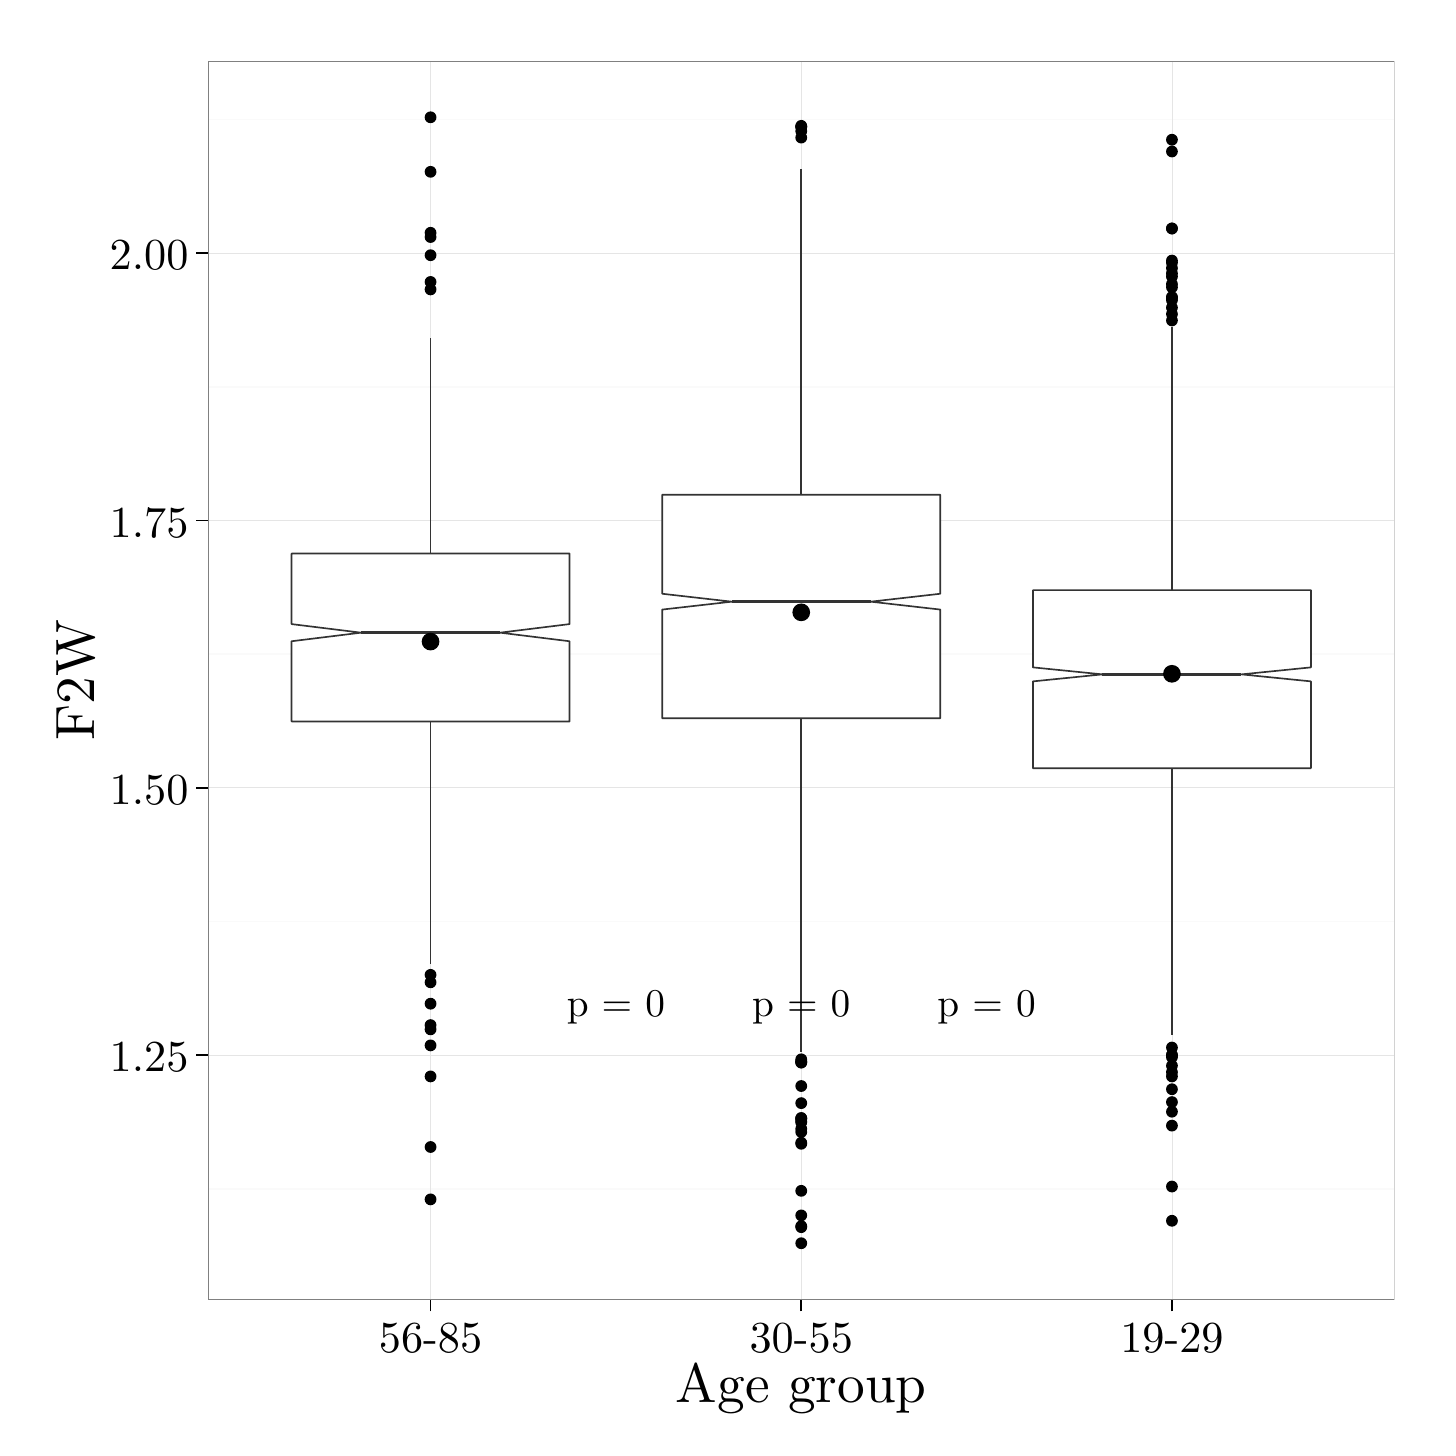
\begin{tikzpicture}[x=1pt,y=1pt]
\definecolor{fillColor}{RGB}{255,255,255}
\path[use as bounding box,fill=fillColor,fill opacity=0.00] (0,0) rectangle (505.89,505.89);
\begin{scope}
\path[clip] (  0.00,  0.00) rectangle (505.89,505.89);
\definecolor{drawColor}{RGB}{255,255,255}
\definecolor{fillColor}{RGB}{255,255,255}

\path[draw=drawColor,line width= 0.6pt,line join=round,line cap=round,fill=fillColor] (  0.00, -0.00) rectangle (505.89,505.89);
\end{scope}
\begin{scope}
\path[clip] ( 65.21, 46.31) rectangle (493.85,493.84);
\definecolor{fillColor}{RGB}{255,255,255}

\path[fill=fillColor] ( 65.21, 46.31) rectangle (493.85,493.84);
\definecolor{drawColor}{gray}{0.98}

\path[draw=drawColor,line width= 0.6pt,line join=round] ( 65.21, 86.36) --
	(493.85, 86.36);

\path[draw=drawColor,line width= 0.6pt,line join=round] ( 65.21,182.95) --
	(493.85,182.95);

\path[draw=drawColor,line width= 0.6pt,line join=round] ( 65.21,279.54) --
	(493.85,279.54);

\path[draw=drawColor,line width= 0.6pt,line join=round] ( 65.21,376.14) --
	(493.85,376.14);

\path[draw=drawColor,line width= 0.6pt,line join=round] ( 65.21,472.73) --
	(493.85,472.73);
\definecolor{drawColor}{gray}{0.90}

\path[draw=drawColor,line width= 0.2pt,line join=round] ( 65.21,134.65) --
	(493.85,134.65);

\path[draw=drawColor,line width= 0.2pt,line join=round] ( 65.21,231.25) --
	(493.85,231.25);

\path[draw=drawColor,line width= 0.2pt,line join=round] ( 65.21,327.84) --
	(493.85,327.84);

\path[draw=drawColor,line width= 0.2pt,line join=round] ( 65.21,424.43) --
	(493.85,424.43);

\path[draw=drawColor,line width= 0.2pt,line join=round] (145.58, 46.31) --
	(145.58,493.84);

\path[draw=drawColor,line width= 0.2pt,line join=round] (279.53, 46.31) --
	(279.53,493.84);

\path[draw=drawColor,line width= 0.2pt,line join=round] (413.48, 46.31) --
	(413.48,493.84);
\definecolor{fillColor}{RGB}{0,0,0}

\path[fill=fillColor] (145.58,126.92) circle (  2.13);

\path[fill=fillColor] (145.58,145.47) circle (  2.13);

\path[fill=fillColor] (145.58,431.77) circle (  2.13);

\path[fill=fillColor] (145.58,411.30) circle (  2.13);

\path[fill=fillColor] (145.58,453.80) circle (  2.13);

\path[fill=fillColor] (145.58,423.66) circle (  2.13);

\path[fill=fillColor] (145.58,153.20) circle (  2.13);

\path[fill=fillColor] (145.58,430.23) circle (  2.13);

\path[fill=fillColor] (145.58,414.00) circle (  2.13);

\path[fill=fillColor] (145.58,143.93) circle (  2.13);

\path[fill=fillColor] (145.58,473.50) circle (  2.13);

\path[fill=fillColor] (145.58, 82.49) circle (  2.13);

\path[fill=fillColor] (145.58,101.42) circle (  2.13);

\path[fill=fillColor] (145.58,163.63) circle (  2.13);

\path[fill=fillColor] (145.58,160.93) circle (  2.13);

\path[fill=fillColor] (145.58,138.13) circle (  2.13);
\definecolor{drawColor}{gray}{0.20}

\path[draw=drawColor,line width= 0.6pt,line join=round] (145.58,315.86) -- (145.58,393.91);

\path[draw=drawColor,line width= 0.6pt,line join=round] (145.58,255.20) -- (145.58,167.49);
\definecolor{fillColor}{RGB}{255,255,255}

\path[draw=drawColor,line width= 0.6pt,line join=round,line cap=round,fill=fillColor] ( 95.35,315.86) --
	( 95.35,290.37) --
	(120.47,287.27) --
	( 95.35,284.17) --
	( 95.35,255.20) --
	(195.81,255.20) --
	(195.81,284.17) --
	(170.70,287.27) --
	(195.81,290.37) --
	(195.81,315.86) --
	( 95.35,315.86) --
	cycle;

\path[draw=drawColor,line width= 1.1pt,line join=round] (120.47,287.27) -- (170.70,287.27);
\definecolor{fillColor}{RGB}{0,0,0}

\path[fill=fillColor] (279.53,132.33) circle (  2.13);

\path[fill=fillColor] (279.53,111.86) circle (  2.13);

\path[fill=fillColor] (279.53,110.31) circle (  2.13);

\path[fill=fillColor] (279.53,107.99) circle (  2.13);

\path[fill=fillColor] (279.53,132.33) circle (  2.13);

\path[fill=fillColor] (279.53,106.83) circle (  2.13);

\path[fill=fillColor] (279.53,468.48) circle (  2.13);

\path[fill=fillColor] (279.53, 85.58) circle (  2.13);

\path[fill=fillColor] (279.53,470.03) circle (  2.13);

\path[fill=fillColor] (279.53,470.03) circle (  2.13);

\path[fill=fillColor] (279.53,470.41) circle (  2.13);

\path[fill=fillColor] (279.53,466.16) circle (  2.13);

\path[fill=fillColor] (279.53, 72.45) circle (  2.13);

\path[fill=fillColor] (279.53,110.70) circle (  2.13);

\path[fill=fillColor] (279.53,111.47) circle (  2.13);

\path[fill=fillColor] (279.53,111.86) circle (  2.13);

\path[fill=fillColor] (279.53,117.27) circle (  2.13);

\path[fill=fillColor] (279.53,102.97) circle (  2.13);

\path[fill=fillColor] (279.53, 72.83) circle (  2.13);

\path[fill=fillColor] (279.53,131.95) circle (  2.13);

\path[fill=fillColor] (279.53,102.58) circle (  2.13);

\path[fill=fillColor] (279.53, 66.65) circle (  2.13);

\path[fill=fillColor] (279.53,131.95) circle (  2.13);

\path[fill=fillColor] (279.53, 76.70) circle (  2.13);

\path[fill=fillColor] (279.53,133.11) circle (  2.13);

\path[fill=fillColor] (279.53,123.45) circle (  2.13);

\path[draw=drawColor,line width= 0.6pt,line join=round] (279.53,337.11) -- (279.53,454.96);

\path[draw=drawColor,line width= 0.6pt,line join=round] (279.53,256.36) -- (279.53,135.81);
\definecolor{fillColor}{RGB}{255,255,255}

\path[draw=drawColor,line width= 0.6pt,line join=round,line cap=round,fill=fillColor] (229.30,337.11) --
	(229.30,301.33) --
	(254.41,298.47) --
	(229.30,295.62) --
	(229.30,256.36) --
	(329.76,256.36) --
	(329.76,295.62) --
	(304.64,298.47) --
	(329.76,301.33) --
	(329.76,337.11) --
	(229.30,337.11) --
	cycle;

\path[draw=drawColor,line width= 1.1pt,line join=round] (254.41,298.47) -- (304.64,298.47);
\definecolor{fillColor}{RGB}{0,0,0}

\path[fill=fillColor] (413.48,134.65) circle (  2.13);

\path[fill=fillColor] (413.48,137.36) circle (  2.13);

\path[fill=fillColor] (413.48,133.88) circle (  2.13);

\path[fill=fillColor] (413.48,413.23) circle (  2.13);

\path[fill=fillColor] (413.48,433.32) circle (  2.13);

\path[fill=fillColor] (413.48,404.73) circle (  2.13);

\path[fill=fillColor] (413.48,402.41) circle (  2.13);

\path[fill=fillColor] (413.48,412.07) circle (  2.13);

\path[fill=fillColor] (413.48,400.09) circle (  2.13);

\path[fill=fillColor] (413.48,114.17) circle (  2.13);

\path[fill=fillColor] (413.48,128.47) circle (  2.13);

\path[fill=fillColor] (413.48,408.59) circle (  2.13);

\path[fill=fillColor] (413.48,407.43) circle (  2.13);

\path[fill=fillColor] (413.48,417.09) circle (  2.13);

\path[fill=fillColor] (413.48,415.93) circle (  2.13);

\path[fill=fillColor] (413.48,419.02) circle (  2.13);

\path[fill=fillColor] (413.48,130.79) circle (  2.13);

\path[fill=fillColor] (413.48,408.21) circle (  2.13);

\path[fill=fillColor] (413.48,461.14) circle (  2.13);

\path[fill=fillColor] (413.48,420.96) circle (  2.13);

\path[fill=fillColor] (413.48,433.32) circle (  2.13);

\path[fill=fillColor] (413.48,465.39) circle (  2.13);

\path[fill=fillColor] (413.48,421.73) circle (  2.13);

\path[fill=fillColor] (413.48,126.92) circle (  2.13);

\path[fill=fillColor] (413.48,109.15) circle (  2.13);

\path[fill=fillColor] (413.48, 74.76) circle (  2.13);

\path[fill=fillColor] (413.48,117.65) circle (  2.13);

\path[fill=fillColor] (413.48,134.65) circle (  2.13);

\path[fill=fillColor] (413.48,122.29) circle (  2.13);

\path[fill=fillColor] (413.48, 87.13) circle (  2.13);

\path[draw=drawColor,line width= 0.6pt,line join=round] (413.48,302.63) -- (413.48,397.77);

\path[draw=drawColor,line width= 0.6pt,line join=round] (413.48,238.30) -- (413.48,141.99);
\definecolor{fillColor}{RGB}{255,255,255}

\path[draw=drawColor,line width= 0.6pt,line join=round,line cap=round,fill=fillColor] (363.25,302.63) --
	(363.25,274.73) --
	(388.36,272.20) --
	(363.25,269.67) --
	(363.25,238.30) --
	(463.71,238.30) --
	(463.71,269.67) --
	(438.59,272.20) --
	(463.71,274.73) --
	(463.71,302.63) --
	(363.25,302.63) --
	cycle;

\path[draw=drawColor,line width= 1.1pt,line join=round] (388.36,272.20) -- (438.59,272.20);
\definecolor{fillColor}{RGB}{0,0,0}

\path[fill=fillColor] (145.58,284.05) circle (  3.20);

\path[fill=fillColor] (279.53,294.62) circle (  3.20);

\path[fill=fillColor] (413.48,272.41) circle (  3.20);
\definecolor{drawColor}{RGB}{0,0,0}

\node[text=drawColor,anchor=base,inner sep=0pt, outer sep=0pt, scale=  1.42] at (212.56,148.63) {p = 0};

\node[text=drawColor,anchor=base,inner sep=0pt, outer sep=0pt, scale=  1.42] at (346.50,148.63) {p = 0};

\node[text=drawColor,anchor=base,inner sep=0pt, outer sep=0pt, scale=  1.42] at (279.53,148.63) {p = 0};
\definecolor{drawColor}{gray}{0.50}

\path[draw=drawColor,line width= 0.6pt,line join=round,line cap=round] ( 65.21, 46.31) rectangle (493.85,493.84);
\end{scope}
\begin{scope}
\path[clip] (  0.00,  0.00) rectangle (505.89,505.89);
\definecolor{drawColor}{RGB}{0,0,0}

\node[text=drawColor,anchor=base east,inner sep=0pt, outer sep=0pt, scale=  1.60] at ( 58.10,128.62) {1.25};

\node[text=drawColor,anchor=base east,inner sep=0pt, outer sep=0pt, scale=  1.60] at ( 58.10,225.21) {1.50};

\node[text=drawColor,anchor=base east,inner sep=0pt, outer sep=0pt, scale=  1.60] at ( 58.10,321.81) {1.75};

\node[text=drawColor,anchor=base east,inner sep=0pt, outer sep=0pt, scale=  1.60] at ( 58.10,418.40) {2.00};
\end{scope}
\begin{scope}
\path[clip] (  0.00,  0.00) rectangle (505.89,505.89);
\definecolor{drawColor}{RGB}{0,0,0}

\path[draw=drawColor,line width= 0.6pt,line join=round] ( 60.95,134.65) --
	( 65.21,134.65);

\path[draw=drawColor,line width= 0.6pt,line join=round] ( 60.95,231.25) --
	( 65.21,231.25);

\path[draw=drawColor,line width= 0.6pt,line join=round] ( 60.95,327.84) --
	( 65.21,327.84);

\path[draw=drawColor,line width= 0.6pt,line join=round] ( 60.95,424.43) --
	( 65.21,424.43);
\end{scope}
\begin{scope}
\path[clip] (  0.00,  0.00) rectangle (505.89,505.89);
\definecolor{drawColor}{RGB}{0,0,0}

\path[draw=drawColor,line width= 0.6pt,line join=round] (145.58, 42.04) --
	(145.58, 46.31);

\path[draw=drawColor,line width= 0.6pt,line join=round] (279.53, 42.04) --
	(279.53, 46.31);

\path[draw=drawColor,line width= 0.6pt,line join=round] (413.48, 42.04) --
	(413.48, 46.31);
\end{scope}
\begin{scope}
\path[clip] (  0.00,  0.00) rectangle (505.89,505.89);
\definecolor{drawColor}{RGB}{0,0,0}

\node[text=drawColor,anchor=base,inner sep=0pt, outer sep=0pt, scale=  1.60] at (145.58, 27.13) {56-85};

\node[text=drawColor,anchor=base,inner sep=0pt, outer sep=0pt, scale=  1.60] at (279.53, 27.13) {30-55};

\node[text=drawColor,anchor=base,inner sep=0pt, outer sep=0pt, scale=  1.60] at (413.48, 27.13) {19-29};
\end{scope}
\begin{scope}
\path[clip] (  0.00,  0.00) rectangle (505.89,505.89);
\definecolor{drawColor}{RGB}{0,0,0}

\node[text=drawColor,anchor=base,inner sep=0pt, outer sep=0pt, scale=  2.00] at (279.53,  9.03) {Age group};
\end{scope}
\begin{scope}
\path[clip] (  0.00,  0.00) rectangle (505.89,505.89);
\definecolor{drawColor}{RGB}{0,0,0}

\node[text=drawColor,rotate= 90.00,anchor=base,inner sep=0pt, outer sep=0pt, scale=  2.00] at ( 24.12,270.08) {F2W};
\end{scope}
\end{tikzpicture}
} 
	\caption{happ\textsc{y} (F2) by age}
	\label{fig.box.f2w.happy.tot}
\end{figure}

I will now turn once more towards the social predictors.
Contrary to the F1 dimension, age of participant is not a significant main effect in the regression model estimating F2 of happ\textsc{y}.
The raw data, on the other hand, paint a different picture.
The box plot (Figure \ref{fig.box.f2w.happy.tot}) shows an increase in mean F2 from the oldest to the middle-aged group: happ\textsc{y} has thus become fronter in this time frame.
While the difference between groups is comparatively small, it is nonetheless highly significant (t(2321.047) = 5.117, p < 0.001).
From the middle to the young group, however, the vowel does not become even more front (i.e. ``more Scouse'' as has been hypothesised), but rather it is centralised again.
The youngest speakers in my sample do not only have happ\textsc{y} realisations that are significantly more central than those of their parents' generation (t(3574.064) = -11.594, p < 0.001).
They use, in fact, variants which are, on average, even more retracted than those of the oldest speakers, a difference which is, once again, highly significant (t(2190.006) = -5.655, p < 0.001).
Just as for F1, I have to conclude that the younger the speaker, the less Scouse --- in this case front --- happ\textsc{y} is.
That being said, it should be kept in mind that age of participant is no longer a significant fixed effect on its own once other factors and random variation due to carrier word are considered.
The same goes for class of subject, even though this factor only just about fails to cross the 5\% threshold.
The interaction of age and social class, however, \emph{is} a significant fixed effect in the regression model.
Figures \ref{fig.box.f2w.happy.ageclass} and \ref{fig.scatter.f2w.happy.ageclass} illustrate the relationship.

\begin{figure}[h!]
	\centering
	\begin{subfigure}{.49\textwidth}
		\centering
			\definecolor{shadecolor}{rgb}{0.969, 0.969, 0.969}
			\resizebox{\linewidth}{!}{% Created by tikzDevice version 0.8.1 on 2016-02-09 02:13:51
% !TEX encoding = UTF-8 Unicode
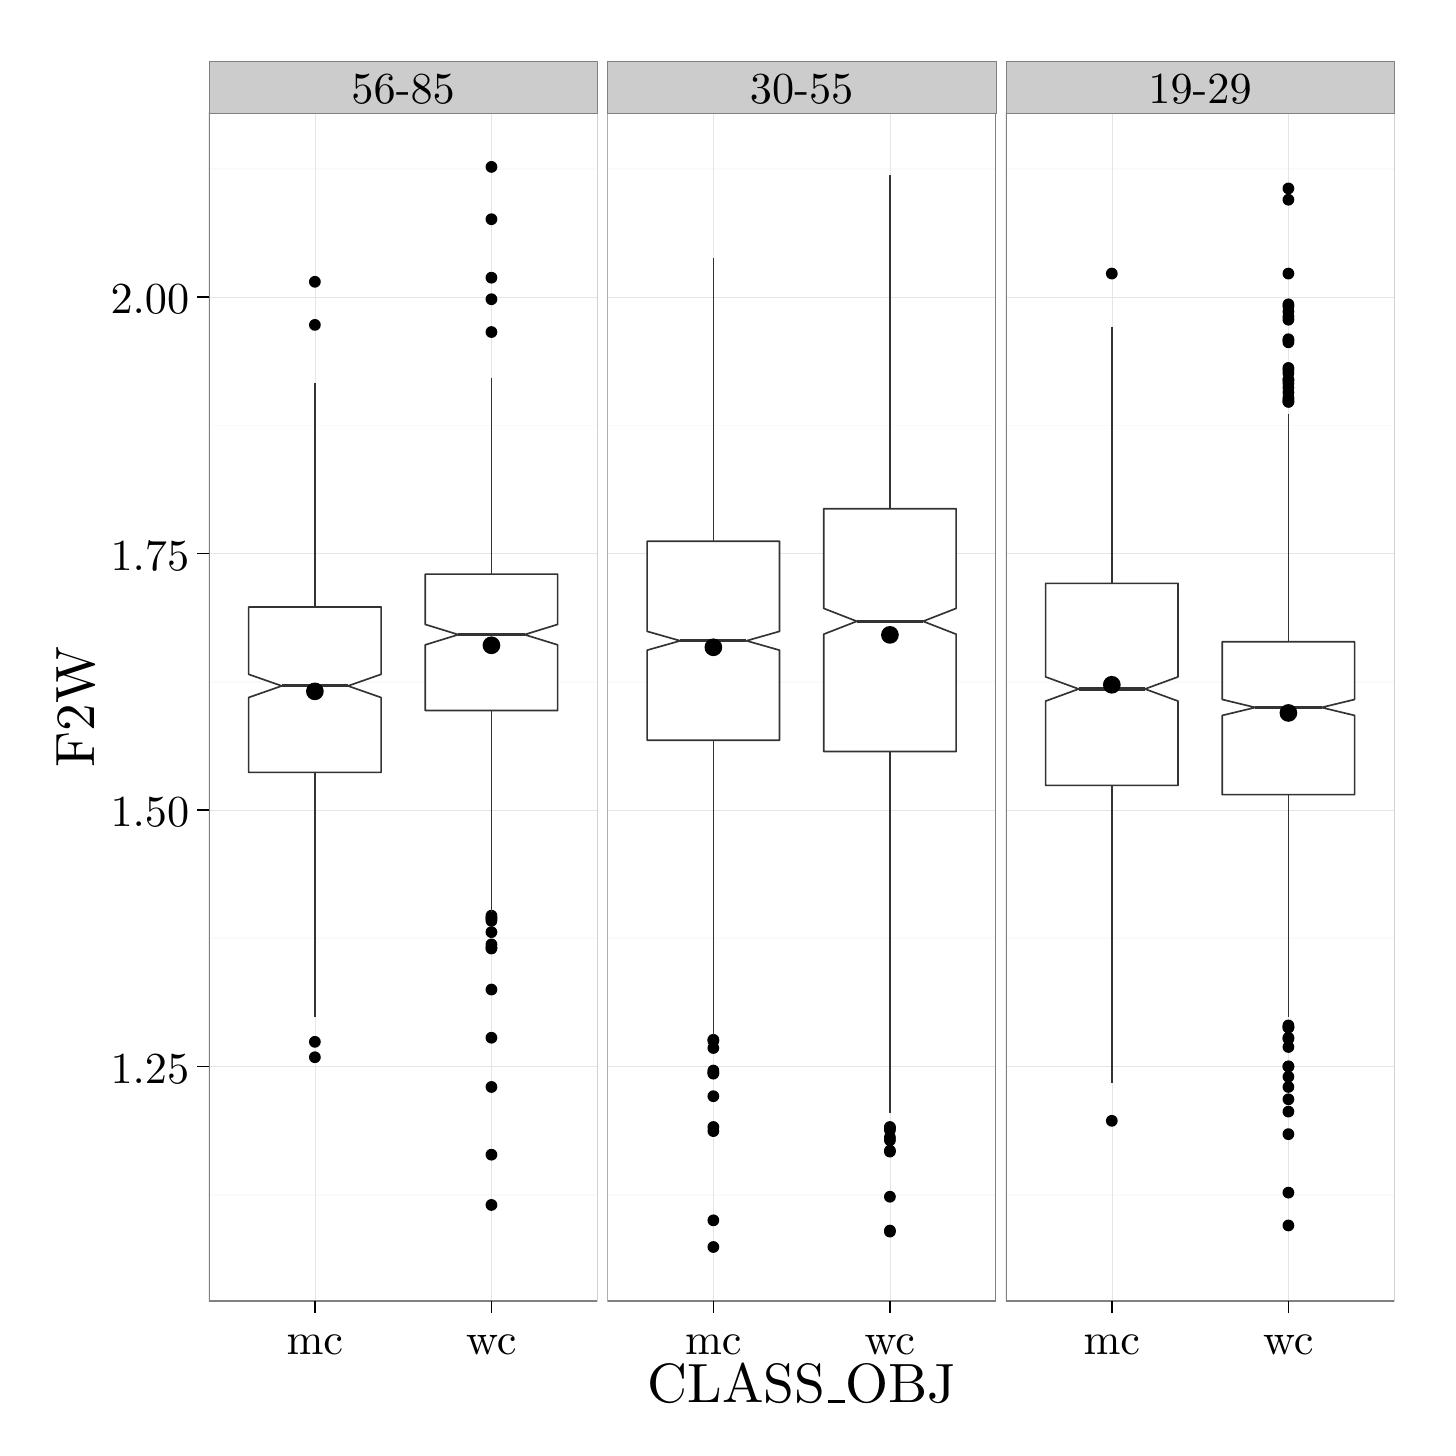
\begin{tikzpicture}[x=1pt,y=1pt]
\definecolor{fillColor}{RGB}{255,255,255}
\path[use as bounding box,fill=fillColor,fill opacity=0.00] (0,0) rectangle (505.89,505.89);
\begin{scope}
\path[clip] (  0.00,  0.00) rectangle (505.89,505.89);
\definecolor{drawColor}{RGB}{255,255,255}
\definecolor{fillColor}{RGB}{255,255,255}

\path[draw=drawColor,line width= 0.6pt,line join=round,line cap=round,fill=fillColor] (  0.00, -0.00) rectangle (505.89,505.89);
\end{scope}
\begin{scope}
\path[clip] ( 65.49, 45.77) rectangle (205.87,475.09);
\definecolor{fillColor}{RGB}{255,255,255}

\path[fill=fillColor] ( 65.49, 45.77) rectangle (205.87,475.09);
\definecolor{drawColor}{gray}{0.98}

\path[draw=drawColor,line width= 0.6pt,line join=round] ( 65.49, 84.19) --
	(205.87, 84.19);

\path[draw=drawColor,line width= 0.6pt,line join=round] ( 65.49,176.85) --
	(205.87,176.85);

\path[draw=drawColor,line width= 0.6pt,line join=round] ( 65.49,269.51) --
	(205.87,269.51);

\path[draw=drawColor,line width= 0.6pt,line join=round] ( 65.49,362.17) --
	(205.87,362.17);

\path[draw=drawColor,line width= 0.6pt,line join=round] ( 65.49,454.83) --
	(205.87,454.83);
\definecolor{drawColor}{gray}{0.90}

\path[draw=drawColor,line width= 0.2pt,line join=round] ( 65.49,130.52) --
	(205.87,130.52);

\path[draw=drawColor,line width= 0.2pt,line join=round] ( 65.49,223.18) --
	(205.87,223.18);

\path[draw=drawColor,line width= 0.2pt,line join=round] ( 65.49,315.84) --
	(205.87,315.84);

\path[draw=drawColor,line width= 0.2pt,line join=round] ( 65.49,408.50) --
	(205.87,408.50);

\path[draw=drawColor,line width= 0.2pt,line join=round] (103.78, 45.77) --
	(103.78,475.09);

\path[draw=drawColor,line width= 0.2pt,line join=round] (167.58, 45.77) --
	(167.58,475.09);
\definecolor{fillColor}{RGB}{0,0,0}

\path[fill=fillColor] (103.78,414.06) circle (  2.13);

\path[fill=fillColor] (103.78,398.49) circle (  2.13);

\path[fill=fillColor] (103.78,139.41) circle (  2.13);

\path[fill=fillColor] (103.78,133.86) circle (  2.13);
\definecolor{drawColor}{gray}{0.20}

\path[draw=drawColor,line width= 0.6pt,line join=round] (103.78,296.57) -- (103.78,377.37);

\path[draw=drawColor,line width= 0.6pt,line join=round] (103.78,236.80) -- (103.78,148.31);
\definecolor{fillColor}{RGB}{255,255,255}

\path[draw=drawColor,line width= 0.6pt,line join=round,line cap=round,fill=fillColor] ( 79.85,296.57) --
	( 79.85,272.22) --
	( 91.81,268.03) --
	( 79.85,263.84) --
	( 79.85,236.80) --
	(127.71,236.80) --
	(127.71,263.84) --
	(115.74,268.03) --
	(127.71,272.22) --
	(127.71,296.57) --
	( 79.85,296.57) --
	cycle;

\path[draw=drawColor,line width= 1.1pt,line join=round] ( 91.81,268.03) -- (115.74,268.03);
\definecolor{fillColor}{RGB}{0,0,0}

\path[fill=fillColor] (167.58,185.00) circle (  2.13);

\path[fill=fillColor] (167.58,184.26) circle (  2.13);

\path[fill=fillColor] (167.58,123.11) circle (  2.13);

\path[fill=fillColor] (167.58,183.89) circle (  2.13);

\path[fill=fillColor] (167.58,179.07) circle (  2.13);

\path[fill=fillColor] (167.58,140.90) circle (  2.13);

\path[fill=fillColor] (167.58,174.63) circle (  2.13);

\path[fill=fillColor] (167.58,173.51) circle (  2.13);

\path[fill=fillColor] (167.58,415.54) circle (  2.13);

\path[fill=fillColor] (167.58,395.90) circle (  2.13);

\path[fill=fillColor] (167.58,436.67) circle (  2.13);

\path[fill=fillColor] (167.58,407.76) circle (  2.13);

\path[fill=fillColor] (167.58,455.57) circle (  2.13);

\path[fill=fillColor] (167.58, 80.48) circle (  2.13);

\path[fill=fillColor] (167.58,173.14) circle (  2.13);

\path[fill=fillColor] (167.58, 98.64) circle (  2.13);

\path[fill=fillColor] (167.58,158.32) circle (  2.13);

\path[fill=fillColor] (167.58,183.15) circle (  2.13);

\path[draw=drawColor,line width= 0.6pt,line join=round] (167.58,308.43) -- (167.58,379.22);

\path[draw=drawColor,line width= 0.6pt,line join=round] (167.58,259.13) -- (167.58,186.49);
\definecolor{fillColor}{RGB}{255,255,255}

\path[draw=drawColor,line width= 0.6pt,line join=round,line cap=round,fill=fillColor] (143.66,308.43) --
	(143.66,290.25) --
	(155.62,286.56) --
	(143.66,282.87) --
	(143.66,259.13) --
	(191.51,259.13) --
	(191.51,282.87) --
	(179.55,286.56) --
	(191.51,290.25) --
	(191.51,308.43) --
	(143.66,308.43) --
	cycle;

\path[draw=drawColor,line width= 1.1pt,line join=round] (155.62,286.56) -- (179.55,286.56);
\definecolor{fillColor}{RGB}{0,0,0}

\path[fill=fillColor] (103.78,266.06) circle (  3.20);

\path[fill=fillColor] (167.58,282.71) circle (  3.20);
\definecolor{drawColor}{gray}{0.50}

\path[draw=drawColor,line width= 0.6pt,line join=round,line cap=round] ( 65.49, 45.77) rectangle (205.87,475.09);
\end{scope}
\begin{scope}
\path[clip] (209.48, 45.77) rectangle (349.86,475.09);
\definecolor{fillColor}{RGB}{255,255,255}

\path[fill=fillColor] (209.48, 45.77) rectangle (349.86,475.09);
\definecolor{drawColor}{gray}{0.98}

\path[draw=drawColor,line width= 0.6pt,line join=round] (209.48, 84.19) --
	(349.86, 84.19);

\path[draw=drawColor,line width= 0.6pt,line join=round] (209.48,176.85) --
	(349.86,176.85);

\path[draw=drawColor,line width= 0.6pt,line join=round] (209.48,269.51) --
	(349.86,269.51);

\path[draw=drawColor,line width= 0.6pt,line join=round] (209.48,362.17) --
	(349.86,362.17);

\path[draw=drawColor,line width= 0.6pt,line join=round] (209.48,454.83) --
	(349.86,454.83);
\definecolor{drawColor}{gray}{0.90}

\path[draw=drawColor,line width= 0.2pt,line join=round] (209.48,130.52) --
	(349.86,130.52);

\path[draw=drawColor,line width= 0.2pt,line join=round] (209.48,223.18) --
	(349.86,223.18);

\path[draw=drawColor,line width= 0.2pt,line join=round] (209.48,315.84) --
	(349.86,315.84);

\path[draw=drawColor,line width= 0.2pt,line join=round] (209.48,408.50) --
	(349.86,408.50);

\path[draw=drawColor,line width= 0.2pt,line join=round] (247.77, 45.77) --
	(247.77,475.09);

\path[draw=drawColor,line width= 0.2pt,line join=round] (311.57, 45.77) --
	(311.57,475.09);
\definecolor{fillColor}{RGB}{0,0,0}

\path[fill=fillColor] (247.77,128.30) circle (  2.13);

\path[fill=fillColor] (247.77,140.16) circle (  2.13);

\path[fill=fillColor] (247.77,108.65) circle (  2.13);

\path[fill=fillColor] (247.77,107.17) circle (  2.13);

\path[fill=fillColor] (247.77,137.19) circle (  2.13);

\path[fill=fillColor] (247.77,139.79) circle (  2.13);

\path[fill=fillColor] (247.77, 65.29) circle (  2.13);

\path[fill=fillColor] (247.77,127.93) circle (  2.13);

\path[fill=fillColor] (247.77, 74.92) circle (  2.13);

\path[fill=fillColor] (247.77,129.04) circle (  2.13);

\path[fill=fillColor] (247.77,119.77) circle (  2.13);
\definecolor{drawColor}{gray}{0.20}

\path[draw=drawColor,line width= 0.6pt,line join=round] (247.77,320.29) -- (247.77,422.59);

\path[draw=drawColor,line width= 0.6pt,line join=round] (247.77,248.38) -- (247.77,142.01);
\definecolor{fillColor}{RGB}{255,255,255}

\path[draw=drawColor,line width= 0.6pt,line join=round,line cap=round,fill=fillColor] (223.84,320.29) --
	(223.84,287.74) --
	(235.80,284.34) --
	(223.84,280.94) --
	(223.84,248.38) --
	(271.69,248.38) --
	(271.69,280.94) --
	(259.73,284.34) --
	(271.69,287.74) --
	(271.69,320.29) --
	(223.84,320.29) --
	cycle;

\path[draw=drawColor,line width= 1.1pt,line join=round] (235.80,284.34) -- (259.73,284.34);
\definecolor{fillColor}{RGB}{0,0,0}

\path[fill=fillColor] (311.57,104.95) circle (  2.13);

\path[fill=fillColor] (311.57,103.83) circle (  2.13);

\path[fill=fillColor] (311.57, 83.45) circle (  2.13);

\path[fill=fillColor] (311.57, 70.85) circle (  2.13);

\path[fill=fillColor] (311.57,107.54) circle (  2.13);

\path[fill=fillColor] (311.57,108.28) circle (  2.13);

\path[fill=fillColor] (311.57,108.65) circle (  2.13);

\path[fill=fillColor] (311.57,100.13) circle (  2.13);

\path[fill=fillColor] (311.57, 71.22) circle (  2.13);

\path[fill=fillColor] (311.57, 99.76) circle (  2.13);

\path[draw=drawColor,line width= 0.6pt,line join=round] (311.57,332.06) -- (311.57,452.61);

\path[draw=drawColor,line width= 0.6pt,line join=round] (311.57,244.31) -- (311.57,113.84);
\definecolor{fillColor}{RGB}{255,255,255}

\path[draw=drawColor,line width= 0.6pt,line join=round,line cap=round,fill=fillColor] (287.65,332.06) --
	(287.65,296.04) --
	(299.61,291.38) --
	(287.65,286.72) --
	(287.65,244.31) --
	(335.50,244.31) --
	(335.50,286.72) --
	(323.54,291.38) --
	(335.50,296.04) --
	(335.50,332.06) --
	(287.65,332.06) --
	cycle;

\path[draw=drawColor,line width= 1.1pt,line join=round] (299.61,291.38) -- (323.54,291.38);
\definecolor{fillColor}{RGB}{0,0,0}

\path[fill=fillColor] (247.77,281.99) circle (  3.20);

\path[fill=fillColor] (311.57,286.47) circle (  3.20);
\definecolor{drawColor}{gray}{0.50}

\path[draw=drawColor,line width= 0.6pt,line join=round,line cap=round] (209.48, 45.77) rectangle (349.86,475.09);
\end{scope}
\begin{scope}
\path[clip] (353.47, 45.77) rectangle (493.84,475.09);
\definecolor{fillColor}{RGB}{255,255,255}

\path[fill=fillColor] (353.47, 45.77) rectangle (493.85,475.09);
\definecolor{drawColor}{gray}{0.98}

\path[draw=drawColor,line width= 0.6pt,line join=round] (353.47, 84.19) --
	(493.84, 84.19);

\path[draw=drawColor,line width= 0.6pt,line join=round] (353.47,176.85) --
	(493.84,176.85);

\path[draw=drawColor,line width= 0.6pt,line join=round] (353.47,269.51) --
	(493.84,269.51);

\path[draw=drawColor,line width= 0.6pt,line join=round] (353.47,362.17) --
	(493.84,362.17);

\path[draw=drawColor,line width= 0.6pt,line join=round] (353.47,454.83) --
	(493.84,454.83);
\definecolor{drawColor}{gray}{0.90}

\path[draw=drawColor,line width= 0.2pt,line join=round] (353.47,130.52) --
	(493.84,130.52);

\path[draw=drawColor,line width= 0.2pt,line join=round] (353.47,223.18) --
	(493.84,223.18);

\path[draw=drawColor,line width= 0.2pt,line join=round] (353.47,315.84) --
	(493.84,315.84);

\path[draw=drawColor,line width= 0.2pt,line join=round] (353.47,408.50) --
	(493.84,408.50);

\path[draw=drawColor,line width= 0.2pt,line join=round] (391.75, 45.77) --
	(391.75,475.09);

\path[draw=drawColor,line width= 0.2pt,line join=round] (455.56, 45.77) --
	(455.56,475.09);
\definecolor{fillColor}{RGB}{0,0,0}

\path[fill=fillColor] (391.75,417.03) circle (  2.13);

\path[fill=fillColor] (391.75,110.88) circle (  2.13);
\definecolor{drawColor}{gray}{0.20}

\path[draw=drawColor,line width= 0.6pt,line join=round] (391.75,305.09) -- (391.75,397.75);

\path[draw=drawColor,line width= 0.6pt,line join=round] (391.75,232.08) -- (391.75,124.59);
\definecolor{fillColor}{RGB}{255,255,255}

\path[draw=drawColor,line width= 0.6pt,line join=round,line cap=round,fill=fillColor] (367.83,305.09) --
	(367.83,271.29) --
	(379.79,266.92) --
	(367.83,262.55) --
	(367.83,232.08) --
	(415.68,232.08) --
	(415.68,262.55) --
	(403.72,266.92) --
	(415.68,271.29) --
	(415.68,305.09) --
	(367.83,305.09) --
	cycle;

\path[draw=drawColor,line width= 1.1pt,line join=round] (379.79,266.92) -- (403.72,266.92);
\definecolor{fillColor}{RGB}{0,0,0}

\path[fill=fillColor] (455.56,130.52) circle (  2.13);

\path[fill=fillColor] (455.56,140.90) circle (  2.13);

\path[fill=fillColor] (455.56,145.35) circle (  2.13);

\path[fill=fillColor] (455.56,393.30) circle (  2.13);

\path[fill=fillColor] (455.56,392.19) circle (  2.13);

\path[fill=fillColor] (455.56,401.46) circle (  2.13);

\path[fill=fillColor] (455.56,400.35) circle (  2.13);

\path[fill=fillColor] (455.56,403.31) circle (  2.13);

\path[fill=fillColor] (455.56,381.07) circle (  2.13);

\path[fill=fillColor] (455.56,126.81) circle (  2.13);

\path[fill=fillColor] (455.56,372.18) circle (  2.13);

\path[fill=fillColor] (455.56,382.19) circle (  2.13);

\path[fill=fillColor] (455.56,392.93) circle (  2.13);

\path[fill=fillColor] (455.56,443.71) circle (  2.13);

\path[fill=fillColor] (455.56,377.37) circle (  2.13);

\path[fill=fillColor] (455.56,405.17) circle (  2.13);

\path[fill=fillColor] (455.56,417.03) circle (  2.13);

\path[fill=fillColor] (455.56,378.48) circle (  2.13);

\path[fill=fillColor] (455.56,144.60) circle (  2.13);

\path[fill=fillColor] (455.56,447.79) circle (  2.13);

\path[fill=fillColor] (455.56,405.91) circle (  2.13);

\path[fill=fillColor] (455.56,370.70) circle (  2.13);

\path[fill=fillColor] (455.56,370.70) circle (  2.13);

\path[fill=fillColor] (455.56,382.93) circle (  2.13);

\path[fill=fillColor] (455.56,378.85) circle (  2.13);

\path[fill=fillColor] (455.56,371.44) circle (  2.13);

\path[fill=fillColor] (455.56,374.03) circle (  2.13);

\path[fill=fillColor] (455.56,123.11) circle (  2.13);

\path[fill=fillColor] (455.56,137.56) circle (  2.13);

\path[fill=fillColor] (455.56,140.53) circle (  2.13);

\path[fill=fillColor] (455.56,106.06) circle (  2.13);

\path[fill=fillColor] (455.56, 73.07) circle (  2.13);

\path[fill=fillColor] (455.56,114.21) circle (  2.13);

\path[fill=fillColor] (455.56,144.60) circle (  2.13);

\path[fill=fillColor] (455.56,130.52) circle (  2.13);

\path[fill=fillColor] (455.56,118.66) circle (  2.13);

\path[fill=fillColor] (455.56,375.88) circle (  2.13);

\path[fill=fillColor] (455.56, 84.93) circle (  2.13);

\path[draw=drawColor,line width= 0.6pt,line join=round] (455.56,283.97) -- (455.56,366.25);

\path[draw=drawColor,line width= 0.6pt,line join=round] (455.56,228.74) -- (455.56,148.31);
\definecolor{fillColor}{RGB}{255,255,255}

\path[draw=drawColor,line width= 0.6pt,line join=round,line cap=round,fill=fillColor] (431.63,283.97) --
	(431.63,263.13) --
	(443.60,260.24) --
	(431.63,257.36) --
	(431.63,228.74) --
	(479.49,228.74) --
	(479.49,257.36) --
	(467.52,260.24) --
	(479.49,263.13) --
	(479.49,283.97) --
	(431.63,283.97) --
	cycle;

\path[draw=drawColor,line width= 1.1pt,line join=round] (443.60,260.24) -- (467.52,260.24);
\definecolor{fillColor}{RGB}{0,0,0}

\path[fill=fillColor] (391.75,268.44) circle (  3.20);

\path[fill=fillColor] (455.56,258.26) circle (  3.20);
\definecolor{drawColor}{gray}{0.50}

\path[draw=drawColor,line width= 0.6pt,line join=round,line cap=round] (353.47, 45.77) rectangle (493.85,475.09);
\end{scope}
\begin{scope}
\path[clip] (  0.00,  0.00) rectangle (505.89,505.89);
\definecolor{drawColor}{gray}{0.50}
\definecolor{fillColor}{gray}{0.80}

\path[draw=drawColor,line width= 0.2pt,line join=round,line cap=round,fill=fillColor] ( 65.49,475.09) rectangle (205.87,493.85);
\definecolor{drawColor}{RGB}{0,0,0}

\node[text=drawColor,anchor=base,inner sep=0pt, outer sep=0pt, scale=  1.60] at (135.68,478.43) {56-85};
\end{scope}
\begin{scope}
\path[clip] (  0.00,  0.00) rectangle (505.89,505.89);
\definecolor{drawColor}{gray}{0.50}
\definecolor{fillColor}{gray}{0.80}

\path[draw=drawColor,line width= 0.2pt,line join=round,line cap=round,fill=fillColor] (209.48,475.09) rectangle (349.86,493.85);
\definecolor{drawColor}{RGB}{0,0,0}

\node[text=drawColor,anchor=base,inner sep=0pt, outer sep=0pt, scale=  1.60] at (279.67,478.43) {30-55};
\end{scope}
\begin{scope}
\path[clip] (  0.00,  0.00) rectangle (505.89,505.89);
\definecolor{drawColor}{gray}{0.50}
\definecolor{fillColor}{gray}{0.80}

\path[draw=drawColor,line width= 0.2pt,line join=round,line cap=round,fill=fillColor] (353.47,475.09) rectangle (493.85,493.85);
\definecolor{drawColor}{RGB}{0,0,0}

\node[text=drawColor,anchor=base,inner sep=0pt, outer sep=0pt, scale=  1.60] at (423.66,478.43) {19-29};
\end{scope}
\begin{scope}
\path[clip] (  0.00,  0.00) rectangle (505.89,505.89);
\definecolor{drawColor}{RGB}{0,0,0}

\node[text=drawColor,anchor=base east,inner sep=0pt, outer sep=0pt, scale=  1.60] at ( 58.38,124.49) {1.25};

\node[text=drawColor,anchor=base east,inner sep=0pt, outer sep=0pt, scale=  1.60] at ( 58.38,217.15) {1.50};

\node[text=drawColor,anchor=base east,inner sep=0pt, outer sep=0pt, scale=  1.60] at ( 58.38,309.81) {1.75};

\node[text=drawColor,anchor=base east,inner sep=0pt, outer sep=0pt, scale=  1.60] at ( 58.38,402.47) {2.00};
\end{scope}
\begin{scope}
\path[clip] (  0.00,  0.00) rectangle (505.89,505.89);
\definecolor{drawColor}{RGB}{0,0,0}

\path[draw=drawColor,line width= 0.6pt,line join=round] ( 61.23,130.52) --
	( 65.49,130.52);

\path[draw=drawColor,line width= 0.6pt,line join=round] ( 61.23,223.18) --
	( 65.49,223.18);

\path[draw=drawColor,line width= 0.6pt,line join=round] ( 61.23,315.84) --
	( 65.49,315.84);

\path[draw=drawColor,line width= 0.6pt,line join=round] ( 61.23,408.50) --
	( 65.49,408.50);
\end{scope}
\begin{scope}
\path[clip] (  0.00,  0.00) rectangle (505.89,505.89);
\definecolor{drawColor}{RGB}{0,0,0}

\path[draw=drawColor,line width= 0.6pt,line join=round] (103.78, 41.50) --
	(103.78, 45.77);

\path[draw=drawColor,line width= 0.6pt,line join=round] (167.58, 41.50) --
	(167.58, 45.77);
\end{scope}
\begin{scope}
\path[clip] (  0.00,  0.00) rectangle (505.89,505.89);
\definecolor{drawColor}{RGB}{0,0,0}

\node[text=drawColor,anchor=base,inner sep=0pt, outer sep=0pt, scale=  1.60] at (103.78, 26.59) {mc};

\node[text=drawColor,anchor=base,inner sep=0pt, outer sep=0pt, scale=  1.60] at (167.58, 26.59) {wc};
\end{scope}
\begin{scope}
\path[clip] (  0.00,  0.00) rectangle (505.89,505.89);
\definecolor{drawColor}{RGB}{0,0,0}

\path[draw=drawColor,line width= 0.6pt,line join=round] (247.77, 41.50) --
	(247.77, 45.77);

\path[draw=drawColor,line width= 0.6pt,line join=round] (311.57, 41.50) --
	(311.57, 45.77);
\end{scope}
\begin{scope}
\path[clip] (  0.00,  0.00) rectangle (505.89,505.89);
\definecolor{drawColor}{RGB}{0,0,0}

\node[text=drawColor,anchor=base,inner sep=0pt, outer sep=0pt, scale=  1.60] at (247.77, 26.59) {mc};

\node[text=drawColor,anchor=base,inner sep=0pt, outer sep=0pt, scale=  1.60] at (311.57, 26.59) {wc};
\end{scope}
\begin{scope}
\path[clip] (  0.00,  0.00) rectangle (505.89,505.89);
\definecolor{drawColor}{RGB}{0,0,0}

\path[draw=drawColor,line width= 0.6pt,line join=round] (391.75, 41.50) --
	(391.75, 45.77);

\path[draw=drawColor,line width= 0.6pt,line join=round] (455.56, 41.50) --
	(455.56, 45.77);
\end{scope}
\begin{scope}
\path[clip] (  0.00,  0.00) rectangle (505.89,505.89);
\definecolor{drawColor}{RGB}{0,0,0}

\node[text=drawColor,anchor=base,inner sep=0pt, outer sep=0pt, scale=  1.60] at (391.75, 26.59) {mc};

\node[text=drawColor,anchor=base,inner sep=0pt, outer sep=0pt, scale=  1.60] at (455.56, 26.59) {wc};
\end{scope}
\begin{scope}
\path[clip] (  0.00,  0.00) rectangle (505.89,505.89);
\definecolor{drawColor}{RGB}{0,0,0}

\node[text=drawColor,anchor=base,inner sep=0pt, outer sep=0pt, scale=  2.00] at (279.67,  9.03) {CLASS{\_{}}OBJ};
\end{scope}
\begin{scope}
\path[clip] (  0.00,  0.00) rectangle (505.89,505.89);
\definecolor{drawColor}{RGB}{0,0,0}

\node[text=drawColor,rotate= 90.00,anchor=base,inner sep=0pt, outer sep=0pt, scale=  2.00] at ( 24.12,260.43) {F2W};
\end{scope}
\end{tikzpicture}
} 
		\caption{box plot}
		\label{fig.box.f2w.happy.ageclass}
	\end{subfigure}
	\begin{subfigure}{.49\textwidth}
		\centering
			\definecolor{shadecolor}{rgb}{0.969, 0.969, 0.969}
			\resizebox{\linewidth}{!}{% Created by tikzDevice version 0.8.1 on 2016-02-09 02:13:53
% !TEX encoding = UTF-8 Unicode
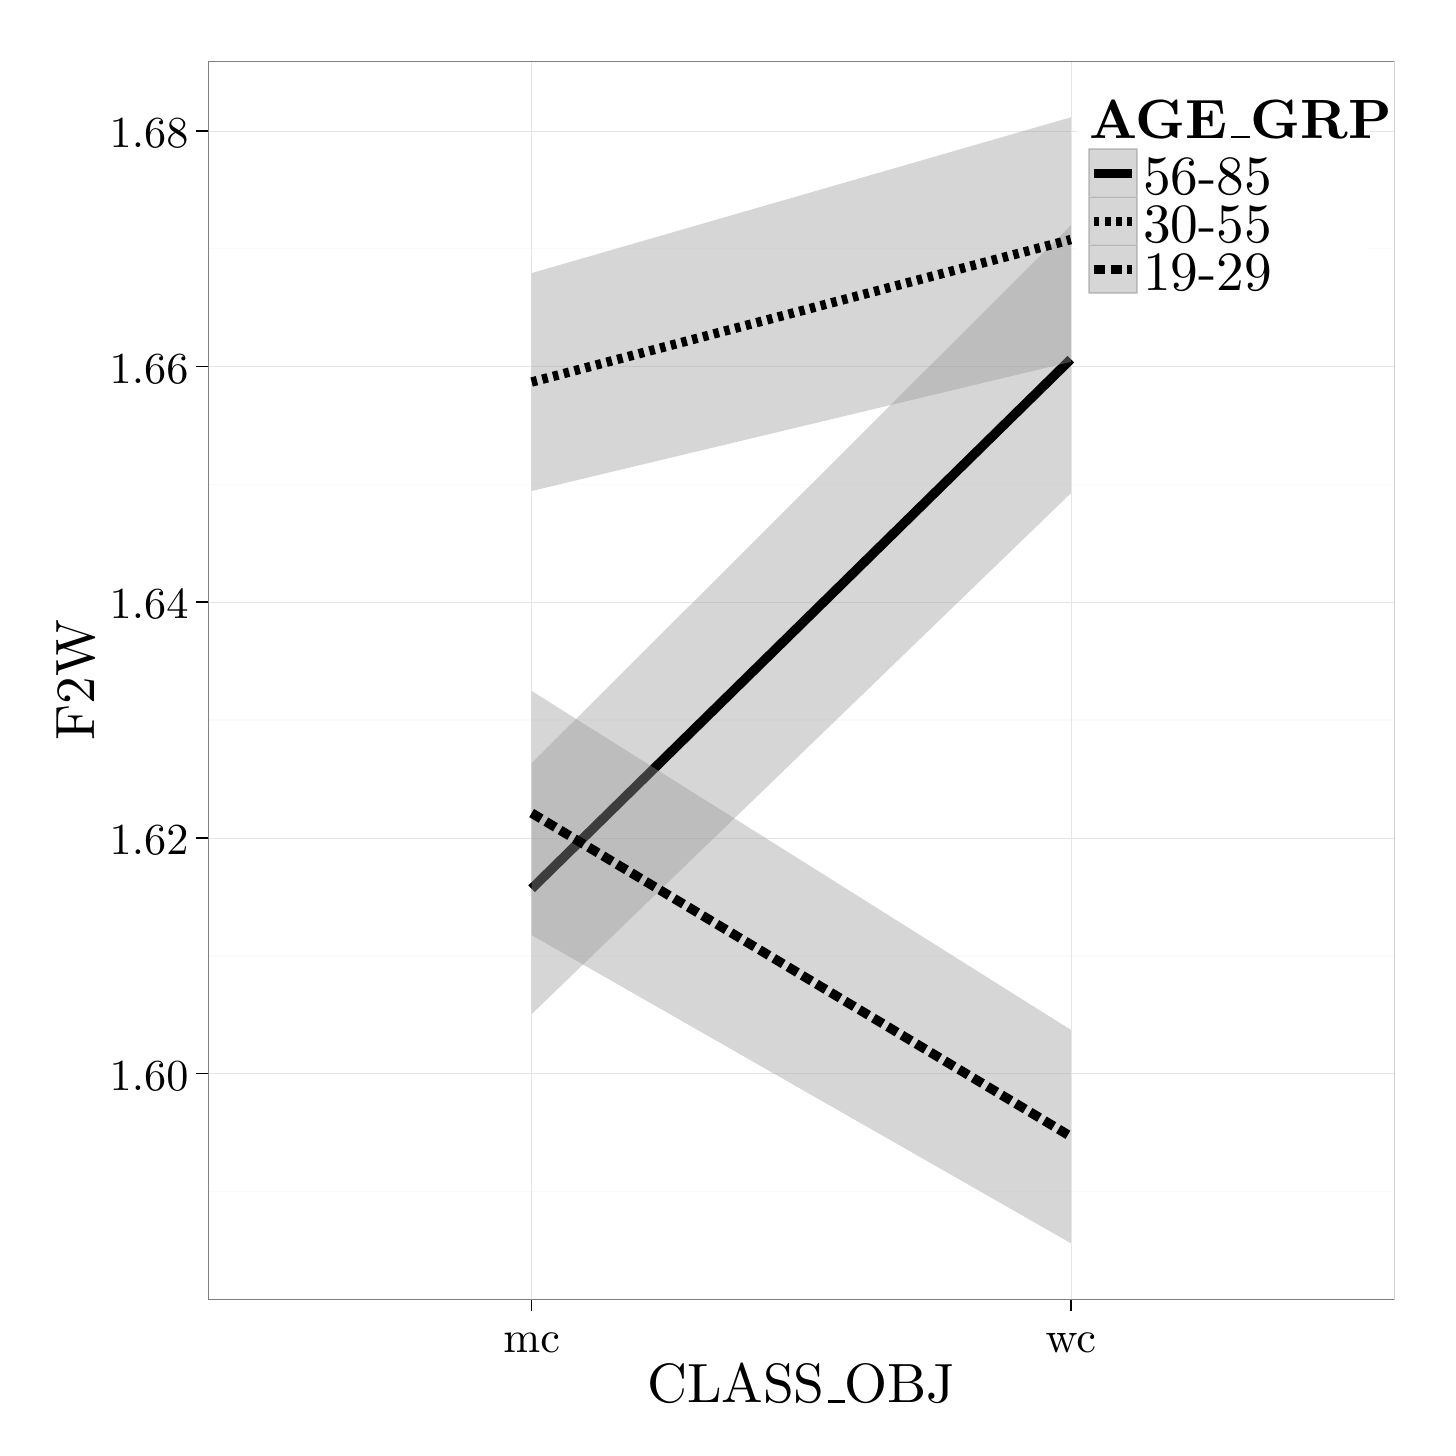
\begin{tikzpicture}[x=1pt,y=1pt]
\definecolor{fillColor}{RGB}{255,255,255}
\path[use as bounding box,fill=fillColor,fill opacity=0.00] (0,0) rectangle (505.89,505.89);
\begin{scope}
\path[clip] (  0.00,  0.00) rectangle (505.89,505.89);
\definecolor{drawColor}{RGB}{255,255,255}
\definecolor{fillColor}{RGB}{255,255,255}

\path[draw=drawColor,line width= 0.6pt,line join=round,line cap=round,fill=fillColor] (  0.00, -0.00) rectangle (505.89,505.89);
\end{scope}
\begin{scope}
\path[clip] ( 65.21, 46.31) rectangle (493.85,493.84);
\definecolor{fillColor}{RGB}{255,255,255}

\path[fill=fillColor] ( 65.21, 46.31) rectangle (493.85,493.84);
\definecolor{drawColor}{gray}{0.98}

\path[draw=drawColor,line width= 0.6pt,line join=round] ( 65.21, 85.38) --
	(493.85, 85.38);

\path[draw=drawColor,line width= 0.6pt,line join=round] ( 65.21,170.54) --
	(493.85,170.54);

\path[draw=drawColor,line width= 0.6pt,line join=round] ( 65.21,255.70) --
	(493.85,255.70);

\path[draw=drawColor,line width= 0.6pt,line join=round] ( 65.21,340.87) --
	(493.85,340.87);

\path[draw=drawColor,line width= 0.6pt,line join=round] ( 65.21,426.03) --
	(493.85,426.03);
\definecolor{drawColor}{gray}{0.90}

\path[draw=drawColor,line width= 0.2pt,line join=round] ( 65.21,127.96) --
	(493.85,127.96);

\path[draw=drawColor,line width= 0.2pt,line join=round] ( 65.21,213.12) --
	(493.85,213.12);

\path[draw=drawColor,line width= 0.2pt,line join=round] ( 65.21,298.28) --
	(493.85,298.28);

\path[draw=drawColor,line width= 0.2pt,line join=round] ( 65.21,383.45) --
	(493.85,383.45);

\path[draw=drawColor,line width= 0.2pt,line join=round] ( 65.21,468.61) --
	(493.85,468.61);

\path[draw=drawColor,line width= 0.2pt,line join=round] (182.11, 46.31) --
	(182.11,493.84);

\path[draw=drawColor,line width= 0.2pt,line join=round] (376.95, 46.31) --
	(376.95,493.84);
\definecolor{fillColor}{RGB}{153,153,153}

\path[fill=fillColor,fill opacity=0.40] (182.11,240.08) --
	(376.95,434.51) --
	(376.95,337.65) --
	(182.11,149.42) --
	cycle;
\definecolor{drawColor}{RGB}{0,0,0}

\path[draw=drawColor,line width= 3.4pt,line join=round] (182.11,194.75) --
	(376.95,386.08);

\path[fill=fillColor,fill opacity=0.40] (182.11,417.21) --
	(376.95,473.50) --
	(376.95,385.12) --
	(182.11,338.46) --
	cycle;

\path[draw=drawColor,line width= 3.4pt,dash pattern=on 2pt off 2pt ,line join=round] (182.11,377.83) --
	(376.95,429.31);

\path[fill=fillColor,fill opacity=0.40] (182.11,266.20) --
	(376.95,143.74) --
	(376.95, 66.65) --
	(182.11,177.97) --
	cycle;

\path[draw=drawColor,line width= 3.4pt,dash pattern=on 4pt off 2pt ,line join=round] (182.11,222.09) --
	(376.95,105.20);
\definecolor{drawColor}{gray}{0.50}

\path[draw=drawColor,line width= 0.6pt,line join=round,line cap=round] ( 65.21, 46.31) rectangle (493.85,493.84);
\end{scope}
\begin{scope}
\path[clip] (  0.00,  0.00) rectangle (505.89,505.89);
\definecolor{drawColor}{RGB}{0,0,0}

\node[text=drawColor,anchor=base east,inner sep=0pt, outer sep=0pt, scale=  1.60] at ( 58.10,121.93) {1.60};

\node[text=drawColor,anchor=base east,inner sep=0pt, outer sep=0pt, scale=  1.60] at ( 58.10,207.09) {1.62};

\node[text=drawColor,anchor=base east,inner sep=0pt, outer sep=0pt, scale=  1.60] at ( 58.10,292.25) {1.64};

\node[text=drawColor,anchor=base east,inner sep=0pt, outer sep=0pt, scale=  1.60] at ( 58.10,377.41) {1.66};

\node[text=drawColor,anchor=base east,inner sep=0pt, outer sep=0pt, scale=  1.60] at ( 58.10,462.57) {1.68};
\end{scope}
\begin{scope}
\path[clip] (  0.00,  0.00) rectangle (505.89,505.89);
\definecolor{drawColor}{RGB}{0,0,0}

\path[draw=drawColor,line width= 0.6pt,line join=round] ( 60.95,127.96) --
	( 65.21,127.96);

\path[draw=drawColor,line width= 0.6pt,line join=round] ( 60.95,213.12) --
	( 65.21,213.12);

\path[draw=drawColor,line width= 0.6pt,line join=round] ( 60.95,298.28) --
	( 65.21,298.28);

\path[draw=drawColor,line width= 0.6pt,line join=round] ( 60.95,383.45) --
	( 65.21,383.45);

\path[draw=drawColor,line width= 0.6pt,line join=round] ( 60.95,468.61) --
	( 65.21,468.61);
\end{scope}
\begin{scope}
\path[clip] (  0.00,  0.00) rectangle (505.89,505.89);
\definecolor{drawColor}{RGB}{0,0,0}

\path[draw=drawColor,line width= 0.6pt,line join=round] (182.11, 42.04) --
	(182.11, 46.31);

\path[draw=drawColor,line width= 0.6pt,line join=round] (376.95, 42.04) --
	(376.95, 46.31);
\end{scope}
\begin{scope}
\path[clip] (  0.00,  0.00) rectangle (505.89,505.89);
\definecolor{drawColor}{RGB}{0,0,0}

\node[text=drawColor,anchor=base,inner sep=0pt, outer sep=0pt, scale=  1.60] at (182.11, 27.13) {mc};

\node[text=drawColor,anchor=base,inner sep=0pt, outer sep=0pt, scale=  1.60] at (376.95, 27.13) {wc};
\end{scope}
\begin{scope}
\path[clip] (  0.00,  0.00) rectangle (505.89,505.89);
\definecolor{drawColor}{RGB}{0,0,0}

\node[text=drawColor,anchor=base,inner sep=0pt, outer sep=0pt, scale=  2.00] at (279.53,  9.03) {CLASS{\_{}}OBJ};
\end{scope}
\begin{scope}
\path[clip] (  0.00,  0.00) rectangle (505.89,505.89);
\definecolor{drawColor}{RGB}{0,0,0}

\node[text=drawColor,rotate= 90.00,anchor=base,inner sep=0pt, outer sep=0pt, scale=  2.00] at ( 24.12,270.08) {F2W};
\end{scope}
\begin{scope}
\path[clip] (  0.00,  0.00) rectangle (505.89,505.89);
\definecolor{fillColor}{RGB}{255,255,255}

\path[fill=fillColor] (379.28,405.66) rectangle (484.98,484.98);
\end{scope}
\begin{scope}
\path[clip] (  0.00,  0.00) rectangle (505.89,505.89);
\definecolor{drawColor}{RGB}{0,0,0}

\node[text=drawColor,anchor=base west,inner sep=0pt, outer sep=0pt, scale=  2.00] at (383.55,465.96) {\bfseries AGE{\_{}}GRP};
\end{scope}
\begin{scope}
\path[clip] (  0.00,  0.00) rectangle (505.89,505.89);
\definecolor{drawColor}{gray}{0.80}
\definecolor{fillColor}{RGB}{255,255,255}

\path[draw=drawColor,line width= 0.6pt,line join=round,line cap=round,fill=fillColor] (383.55,444.61) rectangle (400.89,461.96);
\end{scope}
\begin{scope}
\path[clip] (  0.00,  0.00) rectangle (505.89,505.89);
\definecolor{fillColor}{RGB}{153,153,153}

\path[fill=fillColor,fill opacity=0.40] (383.55,444.61) rectangle (400.89,461.96);
\definecolor{drawColor}{RGB}{0,0,0}

\path[draw=drawColor,line width= 3.4pt,line join=round] (385.28,453.29) -- (399.16,453.29);
\end{scope}
\begin{scope}
\path[clip] (  0.00,  0.00) rectangle (505.89,505.89);
\definecolor{drawColor}{gray}{0.80}
\definecolor{fillColor}{RGB}{255,255,255}

\path[draw=drawColor,line width= 0.6pt,line join=round,line cap=round,fill=fillColor] (383.55,427.27) rectangle (400.89,444.61);
\end{scope}
\begin{scope}
\path[clip] (  0.00,  0.00) rectangle (505.89,505.89);
\definecolor{fillColor}{RGB}{153,153,153}

\path[fill=fillColor,fill opacity=0.40] (383.55,427.27) rectangle (400.89,444.61);
\definecolor{drawColor}{RGB}{0,0,0}

\path[draw=drawColor,line width= 3.4pt,dash pattern=on 2pt off 2pt ,line join=round] (385.28,435.94) -- (399.16,435.94);
\end{scope}
\begin{scope}
\path[clip] (  0.00,  0.00) rectangle (505.89,505.89);
\definecolor{drawColor}{gray}{0.80}
\definecolor{fillColor}{RGB}{255,255,255}

\path[draw=drawColor,line width= 0.6pt,line join=round,line cap=round,fill=fillColor] (383.55,409.92) rectangle (400.89,427.27);
\end{scope}
\begin{scope}
\path[clip] (  0.00,  0.00) rectangle (505.89,505.89);
\definecolor{fillColor}{RGB}{153,153,153}

\path[fill=fillColor,fill opacity=0.40] (383.55,409.92) rectangle (400.89,427.27);
\definecolor{drawColor}{RGB}{0,0,0}

\path[draw=drawColor,line width= 3.4pt,dash pattern=on 4pt off 2pt ,line join=round] (385.28,418.60) -- (399.16,418.60);
\end{scope}
\begin{scope}
\path[clip] (  0.00,  0.00) rectangle (505.89,505.89);
\definecolor{drawColor}{RGB}{0,0,0}

\node[text=drawColor,anchor=base west,inner sep=0pt, outer sep=0pt, scale=  2.00] at (403.06,445.75) {56-85};
\end{scope}
\begin{scope}
\path[clip] (  0.00,  0.00) rectangle (505.89,505.89);
\definecolor{drawColor}{RGB}{0,0,0}

\node[text=drawColor,anchor=base west,inner sep=0pt, outer sep=0pt, scale=  2.00] at (403.06,428.40) {30-55};
\end{scope}
\begin{scope}
\path[clip] (  0.00,  0.00) rectangle (505.89,505.89);
\definecolor{drawColor}{RGB}{0,0,0}

\node[text=drawColor,anchor=base west,inner sep=0pt, outer sep=0pt, scale=  2.00] at (403.06,411.06) {19-29};
\end{scope}
\end{tikzpicture}
} 
		\caption{regression plot}
		\label{fig.scatter.f2w.happy.ageclass}
	\end{subfigure}
	\caption{happ\textsc{y} (F2) by age and class}
\end{figure}

Figure \ref{fig.scatter.f2w.happy.ageclass} shows separate regression lines for the three age groups, which are as usual coded by line type: solid for the oldest, dotted for the middle-aged, and dashed for the youngest speakers.
Estimated F2 is marked on the y-, and social class on the x-axis.
This graph shows two interesting things:
\begin{inparaenum}[(1)]
	\item Class does not only have an effect that is different in degree in the three age groups, but one whose direction is completely reversed in the youngest speakers.
	For both the old and the middle group, working-class speakers use more advanced happ\textsc{y} variants.
	Young working-class speakers, on the other hand, have realisations that are more retracted than those of their middle-class counterparts.
	\item Which age groups are different from each other depends on which social class one looks at.
	In the middle class, the oldest and the youngest speakers appear as one large group, without any significant differences between them (t(1179.969) = 0.836, p = 0.403), but one which does differ greatly from the middle group --- compared to young (t(1446.646) = -5.289, p < 0.001), and old group (t(1127.729) = 6.292, p < 0.001) --- , where realisations are a bit more front.
	Among the working-class speakers, on the other hand, the old and the middle-aged participants form a group, albeit one that shows somewhat more variation (t(1192.156) = 1.219, p = 0.223), which is now significantly different from the youngest speakers --- compared to middle (t(1659.468) = -10.25, p < 0.001), and old group (t(956.457) = -8.952, p < 0.001) ---, who use more retracted variants of happ\textsc{y}.
\end{inparaenum}

The box plot next to this regression plot (\ref{fig.box.f2w.happy.ageclass}) shows the same interaction, but the focus is now more on social class.
There are three panels which illustrate the differences between middle- and working-class speakers within each age group separately.
On the left-hand side one can see that in the oldest age group, working-class subjects have fronter realisations of happ\textsc{y} than the middle-class speakers of the same age group.
The difference looks highly significant (the confidence interval notches do not overlap), and indeed it is (t(929.854) = -5.653, p < 0.001).
In the group of participants who are between 30 and 55 years old, the mean of working-class subjects is also marginally higher, but this time there seems to be much more within-group variation and the two social classes are no longer significantly different from one another (t(1668.574) = -1.663, p = 0.097).
When we look at the youngest speakers, we see again that the trend has reversed (working-class speakers in this subsample have more centralised variants of happ\textsc{y} showing in lower F2 averages), variation --- particularly among working-class subjects --- has decreased and the difference between classes is once more statistically robust (t(1443.946) = 3.878, p < 0.001).
There is thus no straightforward interpretation for either social class or age of participant, because their effects depend on each other not only in terms of degree, but also in direction.
Notwithstanding the slightly confusing picture that these two factors create, one thing seems to be clear when we look at both the means in Figure \ref{fig.box.f2w.happy.ageclass} and the position of the dashed and dotted lines in Figure \ref{fig.scatter.f2w.happy.ageclass}: the youngest subjects in the sample have more retracted happ\textsc{y} realisations than speakers of their parents' generation.
They cannot be said to be more Scouse than their parents or grandparents.

\subsubsection{Style and gender}
\label{sec.prod.res.vow.happy.f2.stylegender}

\begin{figure}[h!]
	\centering
		\definecolor{shadecolor}{rgb}{0.969, 0.969, 0.969}
		\resizebox{.49\linewidth}{!}{% Created by tikzDevice version 0.8.1 on 2016-02-09 02:14:05
% !TEX encoding = UTF-8 Unicode
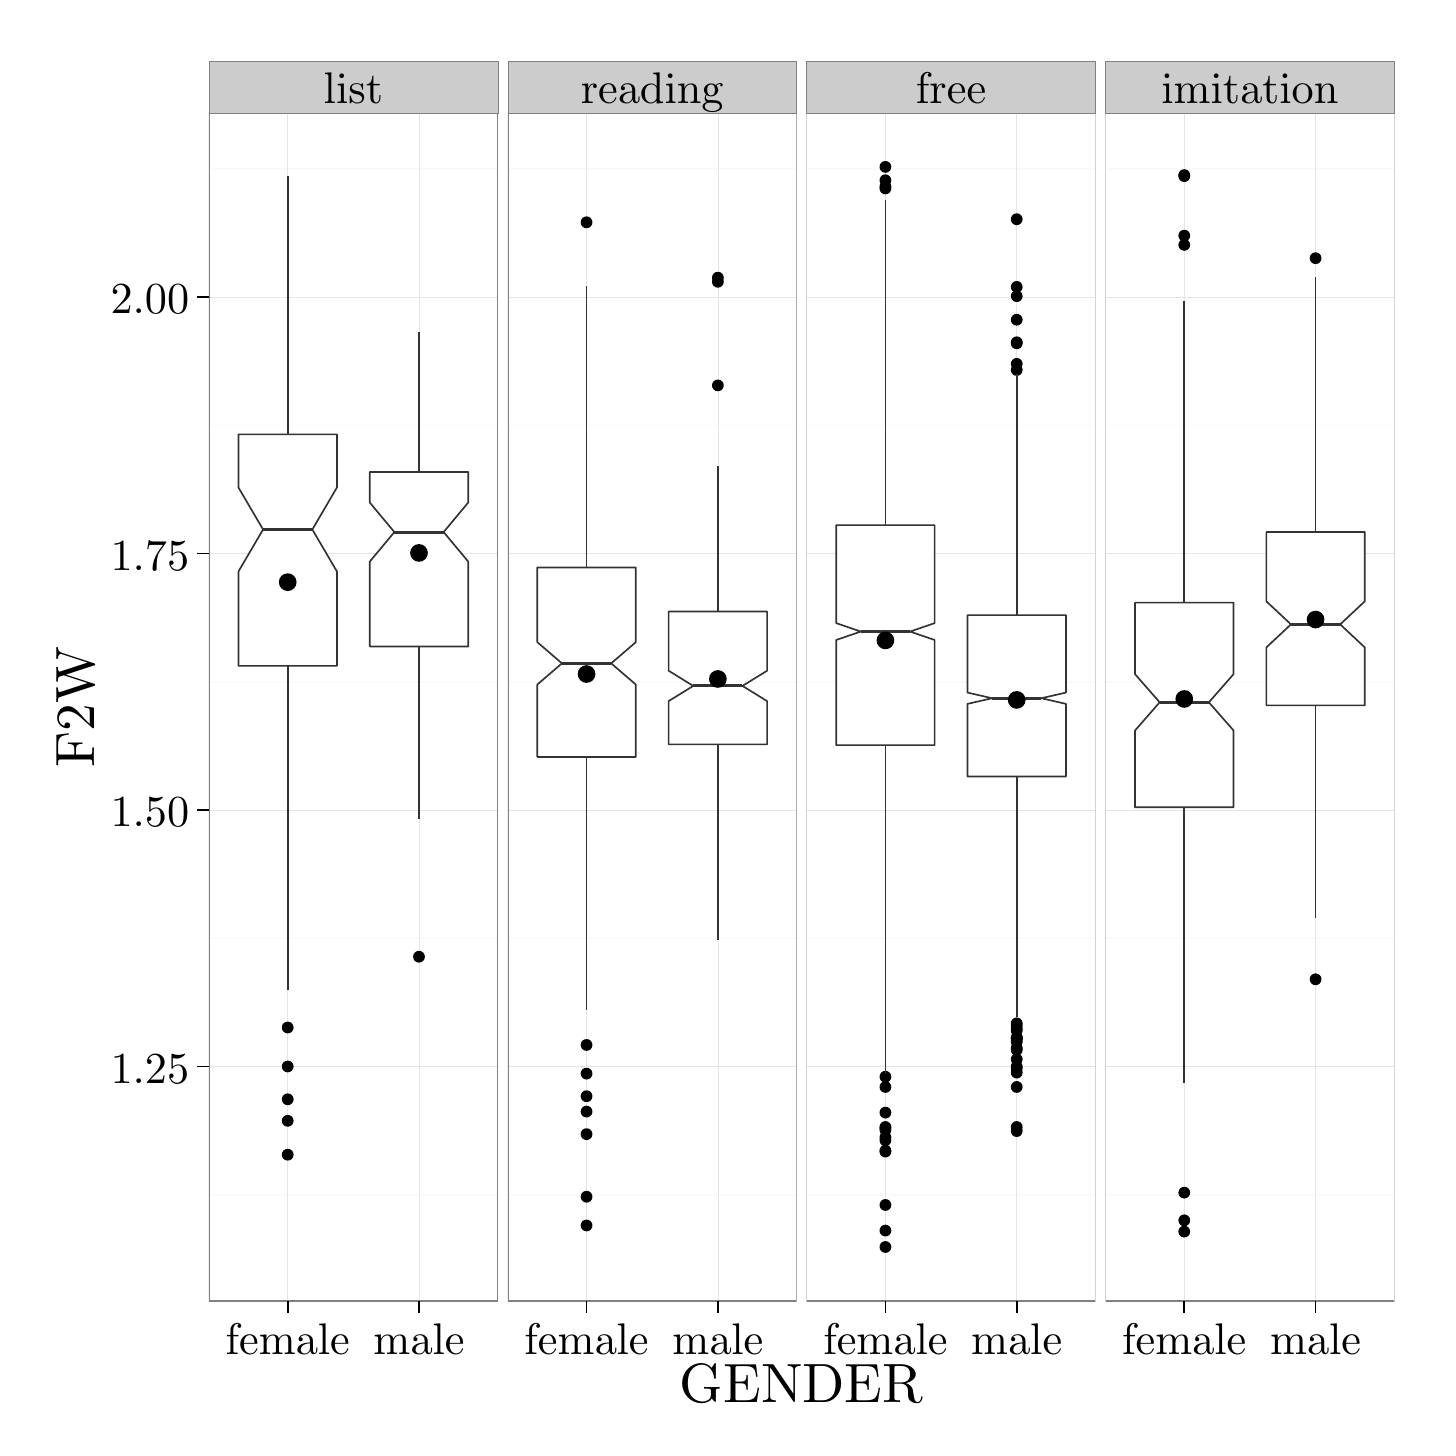
\begin{tikzpicture}[x=1pt,y=1pt]
\definecolor{fillColor}{RGB}{255,255,255}
\path[use as bounding box,fill=fillColor,fill opacity=0.00] (0,0) rectangle (505.89,505.89);
\begin{scope}
\path[clip] (  0.00,  0.00) rectangle (505.89,505.89);
\definecolor{drawColor}{RGB}{255,255,255}
\definecolor{fillColor}{RGB}{255,255,255}

\path[draw=drawColor,line width= 0.6pt,line join=round,line cap=round,fill=fillColor] (  0.00, -0.00) rectangle (505.89,505.89);
\end{scope}
\begin{scope}
\path[clip] ( 65.49, 45.77) rectangle (169.87,475.09);
\definecolor{fillColor}{RGB}{255,255,255}

\path[fill=fillColor] ( 65.49, 45.77) rectangle (169.87,475.09);
\definecolor{drawColor}{gray}{0.98}

\path[draw=drawColor,line width= 0.6pt,line join=round] ( 65.49, 84.19) --
	(169.87, 84.19);

\path[draw=drawColor,line width= 0.6pt,line join=round] ( 65.49,176.85) --
	(169.87,176.85);

\path[draw=drawColor,line width= 0.6pt,line join=round] ( 65.49,269.51) --
	(169.87,269.51);

\path[draw=drawColor,line width= 0.6pt,line join=round] ( 65.49,362.17) --
	(169.87,362.17);

\path[draw=drawColor,line width= 0.6pt,line join=round] ( 65.49,454.83) --
	(169.87,454.83);
\definecolor{drawColor}{gray}{0.90}

\path[draw=drawColor,line width= 0.2pt,line join=round] ( 65.49,130.52) --
	(169.87,130.52);

\path[draw=drawColor,line width= 0.2pt,line join=round] ( 65.49,223.18) --
	(169.87,223.18);

\path[draw=drawColor,line width= 0.2pt,line join=round] ( 65.49,315.84) --
	(169.87,315.84);

\path[draw=drawColor,line width= 0.2pt,line join=round] ( 65.49,408.50) --
	(169.87,408.50);

\path[draw=drawColor,line width= 0.2pt,line join=round] ( 93.96, 45.77) --
	( 93.96,475.09);

\path[draw=drawColor,line width= 0.2pt,line join=round] (141.40, 45.77) --
	(141.40,475.09);
\definecolor{fillColor}{RGB}{0,0,0}

\path[fill=fillColor] ( 93.96,110.88) circle (  2.13);

\path[fill=fillColor] ( 93.96, 98.64) circle (  2.13);

\path[fill=fillColor] ( 93.96,144.60) circle (  2.13);

\path[fill=fillColor] ( 93.96,130.52) circle (  2.13);

\path[fill=fillColor] ( 93.96,118.66) circle (  2.13);
\definecolor{drawColor}{gray}{0.20}

\path[draw=drawColor,line width= 0.6pt,line join=round] ( 93.96,358.93) -- ( 93.96,452.24);

\path[draw=drawColor,line width= 0.6pt,line join=round] ( 93.96,275.26) -- ( 93.96,158.32);
\definecolor{fillColor}{RGB}{255,255,255}

\path[draw=drawColor,line width= 0.6pt,line join=round,line cap=round,fill=fillColor] ( 76.17,358.93) --
	( 76.17,339.72) --
	( 85.06,324.55) --
	( 76.17,309.39) --
	( 76.17,275.26) --
	(111.75,275.26) --
	(111.75,309.39) --
	(102.86,324.55) --
	(111.75,339.72) --
	(111.75,358.93) --
	( 76.17,358.93) --
	cycle;

\path[draw=drawColor,line width= 1.1pt,line join=round] ( 85.06,324.55) -- (102.86,324.55);
\definecolor{fillColor}{RGB}{0,0,0}

\path[fill=fillColor] (141.40,170.18) circle (  2.13);

\path[draw=drawColor,line width= 0.6pt,line join=round] (141.40,345.31) -- (141.40,395.90);

\path[draw=drawColor,line width= 0.6pt,line join=round] (141.40,282.30) -- (141.40,219.84);
\definecolor{fillColor}{RGB}{255,255,255}

\path[draw=drawColor,line width= 0.6pt,line join=round,line cap=round,fill=fillColor] (123.61,345.31) --
	(123.61,334.30) --
	(132.51,323.62) --
	(123.61,312.95) --
	(123.61,282.30) --
	(159.20,282.30) --
	(159.20,312.95) --
	(150.30,323.62) --
	(159.20,334.30) --
	(159.20,345.31) --
	(123.61,345.31) --
	cycle;

\path[draw=drawColor,line width= 1.1pt,line join=round] (132.51,323.62) -- (150.30,323.62);
\definecolor{fillColor}{RGB}{0,0,0}

\path[fill=fillColor] ( 93.96,305.52) circle (  3.20);

\path[fill=fillColor] (141.40,316.08) circle (  3.20);
\definecolor{drawColor}{gray}{0.50}

\path[draw=drawColor,line width= 0.6pt,line join=round,line cap=round] ( 65.49, 45.77) rectangle (169.87,475.09);
\end{scope}
\begin{scope}
\path[clip] (173.49, 45.77) rectangle (277.86,475.09);
\definecolor{fillColor}{RGB}{255,255,255}

\path[fill=fillColor] (173.49, 45.77) rectangle (277.86,475.09);
\definecolor{drawColor}{gray}{0.98}

\path[draw=drawColor,line width= 0.6pt,line join=round] (173.49, 84.19) --
	(277.86, 84.19);

\path[draw=drawColor,line width= 0.6pt,line join=round] (173.49,176.85) --
	(277.86,176.85);

\path[draw=drawColor,line width= 0.6pt,line join=round] (173.49,269.51) --
	(277.86,269.51);

\path[draw=drawColor,line width= 0.6pt,line join=round] (173.49,362.17) --
	(277.86,362.17);

\path[draw=drawColor,line width= 0.6pt,line join=round] (173.49,454.83) --
	(277.86,454.83);
\definecolor{drawColor}{gray}{0.90}

\path[draw=drawColor,line width= 0.2pt,line join=round] (173.49,130.52) --
	(277.86,130.52);

\path[draw=drawColor,line width= 0.2pt,line join=round] (173.49,223.18) --
	(277.86,223.18);

\path[draw=drawColor,line width= 0.2pt,line join=round] (173.49,315.84) --
	(277.86,315.84);

\path[draw=drawColor,line width= 0.2pt,line join=round] (173.49,408.50) --
	(277.86,408.50);

\path[draw=drawColor,line width= 0.2pt,line join=round] (201.95, 45.77) --
	(201.95,475.09);

\path[draw=drawColor,line width= 0.2pt,line join=round] (249.40, 45.77) --
	(249.40,475.09);
\definecolor{fillColor}{RGB}{0,0,0}

\path[fill=fillColor] (201.95,138.30) circle (  2.13);

\path[fill=fillColor] (201.95,435.56) circle (  2.13);

\path[fill=fillColor] (201.95, 83.45) circle (  2.13);

\path[fill=fillColor] (201.95,127.93) circle (  2.13);

\path[fill=fillColor] (201.95,119.77) circle (  2.13);

\path[fill=fillColor] (201.95,106.06) circle (  2.13);

\path[fill=fillColor] (201.95, 73.07) circle (  2.13);

\path[fill=fillColor] (201.95,114.21) circle (  2.13);
\definecolor{drawColor}{gray}{0.20}

\path[draw=drawColor,line width= 0.6pt,line join=round] (201.95,310.84) -- (201.95,412.58);

\path[draw=drawColor,line width= 0.6pt,line join=round] (201.95,242.36) -- (201.95,150.90);
\definecolor{fillColor}{RGB}{255,255,255}

\path[draw=drawColor,line width= 0.6pt,line join=round,line cap=round,fill=fillColor] (184.16,310.84) --
	(184.16,283.83) --
	(193.06,276.18) --
	(184.16,268.53) --
	(184.16,242.36) --
	(219.74,242.36) --
	(219.74,268.53) --
	(210.85,276.18) --
	(219.74,283.83) --
	(219.74,310.84) --
	(184.16,310.84) --
	cycle;

\path[draw=drawColor,line width= 1.1pt,line join=round] (193.06,276.18) -- (210.85,276.18);
\definecolor{fillColor}{RGB}{0,0,0}

\path[fill=fillColor] (249.40,376.63) circle (  2.13);

\path[fill=fillColor] (249.40,415.54) circle (  2.13);

\path[fill=fillColor] (249.40,414.06) circle (  2.13);

\path[draw=drawColor,line width= 0.6pt,line join=round] (249.40,294.90) -- (249.40,347.35);

\path[draw=drawColor,line width= 0.6pt,line join=round] (249.40,246.90) -- (249.40,176.11);
\definecolor{fillColor}{RGB}{255,255,255}

\path[draw=drawColor,line width= 0.6pt,line join=round,line cap=round,fill=fillColor] (231.60,294.90) --
	(231.60,273.52) --
	(240.50,268.03) --
	(231.60,262.54) --
	(231.60,246.90) --
	(267.19,246.90) --
	(267.19,262.54) --
	(258.29,268.03) --
	(267.19,273.52) --
	(267.19,294.90) --
	(231.60,294.90) --
	cycle;

\path[draw=drawColor,line width= 1.1pt,line join=round] (240.50,268.03) -- (258.29,268.03);
\definecolor{fillColor}{RGB}{0,0,0}

\path[fill=fillColor] (201.95,272.33) circle (  3.20);

\path[fill=fillColor] (249.40,270.54) circle (  3.20);
\definecolor{drawColor}{gray}{0.50}

\path[draw=drawColor,line width= 0.6pt,line join=round,line cap=round] (173.49, 45.77) rectangle (277.86,475.09);
\end{scope}
\begin{scope}
\path[clip] (281.48, 45.77) rectangle (385.85,475.09);
\definecolor{fillColor}{RGB}{255,255,255}

\path[fill=fillColor] (281.48, 45.77) rectangle (385.85,475.09);
\definecolor{drawColor}{gray}{0.98}

\path[draw=drawColor,line width= 0.6pt,line join=round] (281.48, 84.19) --
	(385.85, 84.19);

\path[draw=drawColor,line width= 0.6pt,line join=round] (281.48,176.85) --
	(385.85,176.85);

\path[draw=drawColor,line width= 0.6pt,line join=round] (281.48,269.51) --
	(385.85,269.51);

\path[draw=drawColor,line width= 0.6pt,line join=round] (281.48,362.17) --
	(385.85,362.17);

\path[draw=drawColor,line width= 0.6pt,line join=round] (281.48,454.83) --
	(385.85,454.83);
\definecolor{drawColor}{gray}{0.90}

\path[draw=drawColor,line width= 0.2pt,line join=round] (281.48,130.52) --
	(385.85,130.52);

\path[draw=drawColor,line width= 0.2pt,line join=round] (281.48,223.18) --
	(385.85,223.18);

\path[draw=drawColor,line width= 0.2pt,line join=round] (281.48,315.84) --
	(385.85,315.84);

\path[draw=drawColor,line width= 0.2pt,line join=round] (281.48,408.50) --
	(385.85,408.50);

\path[draw=drawColor,line width= 0.2pt,line join=round] (309.94, 45.77) --
	(309.94,475.09);

\path[draw=drawColor,line width= 0.2pt,line join=round] (357.39, 45.77) --
	(357.39,475.09);
\definecolor{fillColor}{RGB}{0,0,0}

\path[fill=fillColor] (309.94,104.95) circle (  2.13);

\path[fill=fillColor] (309.94,103.83) circle (  2.13);

\path[fill=fillColor] (309.94,450.75) circle (  2.13);

\path[fill=fillColor] (309.94,448.53) circle (  2.13);

\path[fill=fillColor] (309.94,107.54) circle (  2.13);

\path[fill=fillColor] (309.94,108.28) circle (  2.13);

\path[fill=fillColor] (309.94,108.65) circle (  2.13);

\path[fill=fillColor] (309.94,113.84) circle (  2.13);

\path[fill=fillColor] (309.94,100.13) circle (  2.13);

\path[fill=fillColor] (309.94, 71.22) circle (  2.13);

\path[fill=fillColor] (309.94, 99.76) circle (  2.13);

\path[fill=fillColor] (309.94,455.57) circle (  2.13);

\path[fill=fillColor] (309.94, 80.48) circle (  2.13);

\path[fill=fillColor] (309.94, 65.29) circle (  2.13);

\path[fill=fillColor] (309.94,126.81) circle (  2.13);

\path[fill=fillColor] (309.94,447.79) circle (  2.13);

\path[fill=fillColor] (309.94,123.11) circle (  2.13);
\definecolor{drawColor}{gray}{0.20}

\path[draw=drawColor,line width= 0.6pt,line join=round] (309.94,326.13) -- (309.94,443.71);

\path[draw=drawColor,line width= 0.6pt,line join=round] (309.94,246.62) -- (309.94,127.93);
\definecolor{fillColor}{RGB}{255,255,255}

\path[draw=drawColor,line width= 0.6pt,line join=round,line cap=round,fill=fillColor] (292.15,326.13) --
	(292.15,290.72) --
	(301.05,287.67) --
	(292.15,284.63) --
	(292.15,246.62) --
	(327.73,246.62) --
	(327.73,284.63) --
	(318.84,287.67) --
	(327.73,290.72) --
	(327.73,326.13) --
	(292.15,326.13) --
	cycle;

\path[draw=drawColor,line width= 1.1pt,line join=round] (301.05,287.67) -- (318.84,287.67);
\definecolor{fillColor}{RGB}{0,0,0}

\path[fill=fillColor] (357.39,128.30) circle (  2.13);

\path[fill=fillColor] (357.39,140.16) circle (  2.13);

\path[fill=fillColor] (357.39,130.52) circle (  2.13);

\path[fill=fillColor] (357.39,140.90) circle (  2.13);

\path[fill=fillColor] (357.39,108.65) circle (  2.13);

\path[fill=fillColor] (357.39,107.17) circle (  2.13);

\path[fill=fillColor] (357.39,146.09) circle (  2.13);

\path[fill=fillColor] (357.39,412.21) circle (  2.13);

\path[fill=fillColor] (357.39,137.19) circle (  2.13);

\path[fill=fillColor] (357.39,145.35) circle (  2.13);

\path[fill=fillColor] (357.39,123.11) circle (  2.13);

\path[fill=fillColor] (357.39,140.90) circle (  2.13);

\path[fill=fillColor] (357.39,436.67) circle (  2.13);

\path[fill=fillColor] (357.39,139.41) circle (  2.13);

\path[fill=fillColor] (357.39,144.23) circle (  2.13);

\path[fill=fillColor] (357.39,136.45) circle (  2.13);

\path[fill=fillColor] (357.39,408.87) circle (  2.13);

\path[fill=fillColor] (357.39,392.19) circle (  2.13);

\path[fill=fillColor] (357.39,382.19) circle (  2.13);

\path[fill=fillColor] (357.39,400.35) circle (  2.13);

\path[fill=fillColor] (357.39,391.82) circle (  2.13);

\path[fill=fillColor] (357.39,384.41) circle (  2.13);

\path[fill=fillColor] (357.39,140.90) circle (  2.13);

\path[fill=fillColor] (357.39,143.49) circle (  2.13);

\path[fill=fillColor] (357.39,133.11) circle (  2.13);

\path[fill=fillColor] (357.39,129.78) circle (  2.13);

\path[draw=drawColor,line width= 0.6pt,line join=round] (357.39,293.60) -- (357.39,380.70);

\path[draw=drawColor,line width= 0.6pt,line join=round] (357.39,235.32) -- (357.39,148.31);
\definecolor{fillColor}{RGB}{255,255,255}

\path[draw=drawColor,line width= 0.6pt,line join=round,line cap=round,fill=fillColor] (339.60,293.60) --
	(339.60,265.62) --
	(348.49,263.58) --
	(339.60,261.54) --
	(339.60,235.32) --
	(375.18,235.32) --
	(375.18,261.54) --
	(366.28,263.58) --
	(375.18,265.62) --
	(375.18,293.60) --
	(339.60,293.60) --
	cycle;

\path[draw=drawColor,line width= 1.1pt,line join=round] (348.49,263.58) -- (366.28,263.58);
\definecolor{fillColor}{RGB}{0,0,0}

\path[fill=fillColor] (309.94,284.48) circle (  3.20);

\path[fill=fillColor] (357.39,262.97) circle (  3.20);
\definecolor{drawColor}{gray}{0.50}

\path[draw=drawColor,line width= 0.6pt,line join=round,line cap=round] (281.48, 45.77) rectangle (385.85,475.09);
\end{scope}
\begin{scope}
\path[clip] (389.47, 45.77) rectangle (493.85,475.09);
\definecolor{fillColor}{RGB}{255,255,255}

\path[fill=fillColor] (389.47, 45.77) rectangle (493.85,475.09);
\definecolor{drawColor}{gray}{0.98}

\path[draw=drawColor,line width= 0.6pt,line join=round] (389.47, 84.19) --
	(493.85, 84.19);

\path[draw=drawColor,line width= 0.6pt,line join=round] (389.47,176.85) --
	(493.85,176.85);

\path[draw=drawColor,line width= 0.6pt,line join=round] (389.47,269.51) --
	(493.85,269.51);

\path[draw=drawColor,line width= 0.6pt,line join=round] (389.47,362.17) --
	(493.85,362.17);

\path[draw=drawColor,line width= 0.6pt,line join=round] (389.47,454.83) --
	(493.85,454.83);
\definecolor{drawColor}{gray}{0.90}

\path[draw=drawColor,line width= 0.2pt,line join=round] (389.47,130.52) --
	(493.85,130.52);

\path[draw=drawColor,line width= 0.2pt,line join=round] (389.47,223.18) --
	(493.85,223.18);

\path[draw=drawColor,line width= 0.2pt,line join=round] (389.47,315.84) --
	(493.85,315.84);

\path[draw=drawColor,line width= 0.2pt,line join=round] (389.47,408.50) --
	(493.85,408.50);

\path[draw=drawColor,line width= 0.2pt,line join=round] (417.93, 45.77) --
	(417.93,475.09);

\path[draw=drawColor,line width= 0.2pt,line join=round] (465.38, 45.77) --
	(465.38,475.09);
\definecolor{fillColor}{RGB}{0,0,0}

\path[fill=fillColor] (417.93,452.24) circle (  2.13);

\path[fill=fillColor] (417.93,452.61) circle (  2.13);

\path[fill=fillColor] (417.93,427.40) circle (  2.13);

\path[fill=fillColor] (417.93,430.74) circle (  2.13);

\path[fill=fillColor] (417.93, 70.85) circle (  2.13);

\path[fill=fillColor] (417.93, 74.92) circle (  2.13);

\path[fill=fillColor] (417.93, 84.93) circle (  2.13);
\definecolor{drawColor}{gray}{0.20}

\path[draw=drawColor,line width= 0.6pt,line join=round] (417.93,298.14) -- (417.93,407.02);

\path[draw=drawColor,line width= 0.6pt,line join=round] (417.93,224.20) -- (417.93,124.59);
\definecolor{fillColor}{RGB}{255,255,255}

\path[draw=drawColor,line width= 0.6pt,line join=round,line cap=round,fill=fillColor] (400.14,298.14) --
	(400.14,272.27) --
	(409.04,262.10) --
	(400.14,251.93) --
	(400.14,224.20) --
	(435.73,224.20) --
	(435.73,251.93) --
	(426.83,262.10) --
	(435.73,272.27) --
	(435.73,298.14) --
	(400.14,298.14) --
	cycle;

\path[draw=drawColor,line width= 1.1pt,line join=round] (409.04,262.10) -- (426.83,262.10);
\definecolor{fillColor}{RGB}{0,0,0}

\path[fill=fillColor] (465.38,422.59) circle (  2.13);

\path[fill=fillColor] (465.38,162.02) circle (  2.13);

\path[draw=drawColor,line width= 0.6pt,line join=round] (465.38,323.62) -- (465.38,415.91);

\path[draw=drawColor,line width= 0.6pt,line join=round] (465.38,260.99) -- (465.38,184.26);
\definecolor{fillColor}{RGB}{255,255,255}

\path[draw=drawColor,line width= 0.6pt,line join=round,line cap=round,fill=fillColor] (447.59,323.62) --
	(447.59,298.60) --
	(456.48,290.27) --
	(447.59,281.93) --
	(447.59,260.99) --
	(483.17,260.99) --
	(483.17,281.93) --
	(474.27,290.27) --
	(483.17,298.60) --
	(483.17,323.62) --
	(447.59,323.62) --
	cycle;

\path[draw=drawColor,line width= 1.1pt,line join=round] (456.48,290.27) -- (474.27,290.27);
\definecolor{fillColor}{RGB}{0,0,0}

\path[fill=fillColor] (417.93,263.32) circle (  3.20);

\path[fill=fillColor] (465.38,292.01) circle (  3.20);
\definecolor{drawColor}{gray}{0.50}

\path[draw=drawColor,line width= 0.6pt,line join=round,line cap=round] (389.47, 45.77) rectangle (493.85,475.09);
\end{scope}
\begin{scope}
\path[clip] (  0.00,  0.00) rectangle (505.89,505.89);
\definecolor{drawColor}{gray}{0.50}
\definecolor{fillColor}{gray}{0.80}

\path[draw=drawColor,line width= 0.2pt,line join=round,line cap=round,fill=fillColor] ( 65.49,475.09) rectangle (169.87,493.85);
\definecolor{drawColor}{RGB}{0,0,0}

\node[text=drawColor,anchor=base,inner sep=0pt, outer sep=0pt, scale=  1.60] at (117.68,478.43) {list};
\end{scope}
\begin{scope}
\path[clip] (  0.00,  0.00) rectangle (505.89,505.89);
\definecolor{drawColor}{gray}{0.50}
\definecolor{fillColor}{gray}{0.80}

\path[draw=drawColor,line width= 0.2pt,line join=round,line cap=round,fill=fillColor] (173.49,475.09) rectangle (277.86,493.85);
\definecolor{drawColor}{RGB}{0,0,0}

\node[text=drawColor,anchor=base,inner sep=0pt, outer sep=0pt, scale=  1.60] at (225.67,478.43) {reading};
\end{scope}
\begin{scope}
\path[clip] (  0.00,  0.00) rectangle (505.89,505.89);
\definecolor{drawColor}{gray}{0.50}
\definecolor{fillColor}{gray}{0.80}

\path[draw=drawColor,line width= 0.2pt,line join=round,line cap=round,fill=fillColor] (281.48,475.09) rectangle (385.85,493.85);
\definecolor{drawColor}{RGB}{0,0,0}

\node[text=drawColor,anchor=base,inner sep=0pt, outer sep=0pt, scale=  1.60] at (333.67,478.43) {free};
\end{scope}
\begin{scope}
\path[clip] (  0.00,  0.00) rectangle (505.89,505.89);
\definecolor{drawColor}{gray}{0.50}
\definecolor{fillColor}{gray}{0.80}

\path[draw=drawColor,line width= 0.2pt,line join=round,line cap=round,fill=fillColor] (389.47,475.09) rectangle (493.85,493.85);
\definecolor{drawColor}{RGB}{0,0,0}

\node[text=drawColor,anchor=base,inner sep=0pt, outer sep=0pt, scale=  1.60] at (441.66,478.43) {imitation};
\end{scope}
\begin{scope}
\path[clip] (  0.00,  0.00) rectangle (505.89,505.89);
\definecolor{drawColor}{RGB}{0,0,0}

\node[text=drawColor,anchor=base east,inner sep=0pt, outer sep=0pt, scale=  1.60] at ( 58.38,124.49) {1.25};

\node[text=drawColor,anchor=base east,inner sep=0pt, outer sep=0pt, scale=  1.60] at ( 58.38,217.15) {1.50};

\node[text=drawColor,anchor=base east,inner sep=0pt, outer sep=0pt, scale=  1.60] at ( 58.38,309.81) {1.75};

\node[text=drawColor,anchor=base east,inner sep=0pt, outer sep=0pt, scale=  1.60] at ( 58.38,402.47) {2.00};
\end{scope}
\begin{scope}
\path[clip] (  0.00,  0.00) rectangle (505.89,505.89);
\definecolor{drawColor}{RGB}{0,0,0}

\path[draw=drawColor,line width= 0.6pt,line join=round] ( 61.23,130.52) --
	( 65.49,130.52);

\path[draw=drawColor,line width= 0.6pt,line join=round] ( 61.23,223.18) --
	( 65.49,223.18);

\path[draw=drawColor,line width= 0.6pt,line join=round] ( 61.23,315.84) --
	( 65.49,315.84);

\path[draw=drawColor,line width= 0.6pt,line join=round] ( 61.23,408.50) --
	( 65.49,408.50);
\end{scope}
\begin{scope}
\path[clip] (  0.00,  0.00) rectangle (505.89,505.89);
\definecolor{drawColor}{RGB}{0,0,0}

\path[draw=drawColor,line width= 0.6pt,line join=round] ( 93.96, 41.50) --
	( 93.96, 45.77);

\path[draw=drawColor,line width= 0.6pt,line join=round] (141.40, 41.50) --
	(141.40, 45.77);
\end{scope}
\begin{scope}
\path[clip] (  0.00,  0.00) rectangle (505.89,505.89);
\definecolor{drawColor}{RGB}{0,0,0}

\node[text=drawColor,anchor=base,inner sep=0pt, outer sep=0pt, scale=  1.60] at ( 93.96, 26.59) {female};

\node[text=drawColor,anchor=base,inner sep=0pt, outer sep=0pt, scale=  1.60] at (141.40, 26.59) {male};
\end{scope}
\begin{scope}
\path[clip] (  0.00,  0.00) rectangle (505.89,505.89);
\definecolor{drawColor}{RGB}{0,0,0}

\path[draw=drawColor,line width= 0.6pt,line join=round] (201.95, 41.50) --
	(201.95, 45.77);

\path[draw=drawColor,line width= 0.6pt,line join=round] (249.40, 41.50) --
	(249.40, 45.77);
\end{scope}
\begin{scope}
\path[clip] (  0.00,  0.00) rectangle (505.89,505.89);
\definecolor{drawColor}{RGB}{0,0,0}

\node[text=drawColor,anchor=base,inner sep=0pt, outer sep=0pt, scale=  1.60] at (201.95, 26.59) {female};

\node[text=drawColor,anchor=base,inner sep=0pt, outer sep=0pt, scale=  1.60] at (249.40, 26.59) {male};
\end{scope}
\begin{scope}
\path[clip] (  0.00,  0.00) rectangle (505.89,505.89);
\definecolor{drawColor}{RGB}{0,0,0}

\path[draw=drawColor,line width= 0.6pt,line join=round] (309.94, 41.50) --
	(309.94, 45.77);

\path[draw=drawColor,line width= 0.6pt,line join=round] (357.39, 41.50) --
	(357.39, 45.77);
\end{scope}
\begin{scope}
\path[clip] (  0.00,  0.00) rectangle (505.89,505.89);
\definecolor{drawColor}{RGB}{0,0,0}

\node[text=drawColor,anchor=base,inner sep=0pt, outer sep=0pt, scale=  1.60] at (309.94, 26.59) {female};

\node[text=drawColor,anchor=base,inner sep=0pt, outer sep=0pt, scale=  1.60] at (357.39, 26.59) {male};
\end{scope}
\begin{scope}
\path[clip] (  0.00,  0.00) rectangle (505.89,505.89);
\definecolor{drawColor}{RGB}{0,0,0}

\path[draw=drawColor,line width= 0.6pt,line join=round] (417.93, 41.50) --
	(417.93, 45.77);

\path[draw=drawColor,line width= 0.6pt,line join=round] (465.38, 41.50) --
	(465.38, 45.77);
\end{scope}
\begin{scope}
\path[clip] (  0.00,  0.00) rectangle (505.89,505.89);
\definecolor{drawColor}{RGB}{0,0,0}

\node[text=drawColor,anchor=base,inner sep=0pt, outer sep=0pt, scale=  1.60] at (417.93, 26.59) {female};

\node[text=drawColor,anchor=base,inner sep=0pt, outer sep=0pt, scale=  1.60] at (465.38, 26.59) {male};
\end{scope}
\begin{scope}
\path[clip] (  0.00,  0.00) rectangle (505.89,505.89);
\definecolor{drawColor}{RGB}{0,0,0}

\node[text=drawColor,anchor=base,inner sep=0pt, outer sep=0pt, scale=  2.00] at (279.67,  9.03) {GENDER};
\end{scope}
\begin{scope}
\path[clip] (  0.00,  0.00) rectangle (505.89,505.89);
\definecolor{drawColor}{RGB}{0,0,0}

\node[text=drawColor,rotate= 90.00,anchor=base,inner sep=0pt, outer sep=0pt, scale=  2.00] at ( 24.12,260.43) {F2W};
\end{scope}
\end{tikzpicture}
} 
	\caption{happ\textsc{y} (F2) by style and gender}
	\label{fig.box.f2w.happy.stylegender}
\end{figure}

The second significant interaction in the mixed-effects model, style X gender, is not really simpler in nature.
The box plots in Figure \ref{fig.box.f2w.happy.stylegender} illustrate within-style comparisons by gender, but they also show style differences within genders.
For female speakers (boxes on the left-hand side of each panel), the three styles `reading', `free', and `imitation\is{accent performance}' have relatively similar realisations.
This is especially true for reading and accent perform\is{accent performance}ance, where means are very close and notches overlap.
Table \ref{tab.happy.genderstyle.pvalues} summarises t-tests on the raw data for all possible comparisons of style, separated by gender of subject.
The p-value of 0.22 for reading-imitation\is{accent performance} (females) confirms that these two styles are not significantly different, whereas spontaneous speech differs from both reading (p = 0.008) and imitation\is{accent performance} (p < 0.001) in a statistically robust way.
Realisations of happ\textsc{y} elicited via the word list show slightly more variation around the mean, but are nevertheless clearly distinct from all three remaining styles as both the box plot and the t-tests (cf. Table \ref{tab.happy.genderstyle.pvalues}) suggest.

\begin{table}[h!]
	\centering
	\caption{happ\textsc{y} (F2): t-tests of style by gender}
	\label{tab.happy.genderstyle.pvalues}
	\begin{tabular}{lrrrrrr}
		\hline
		test & \multicolumn{3}{c}{women} & \multicolumn{3}{c}{men}\\
		& t & df & p & t & df & p\\
		\hline
		list-reading & 3.396 & 113.708 & < 0.001 & 8.343 & 165.401 & < 0.001\\
		list-free & 2.370 & 79.086 & 0.020 & 11.426 & 94.870 & < 0.001\\
		list-imitation\is{accent performance} & 3.994 & 141.852 & < 0.001 & 3.984 & 197.933 & < 0.001\\
		reading-free & \ensuremath{-2.661} & 244.712 & 0.008 & 2.362 & 234.779 & 0.019\\
		reading-imitation\is{accent performance} & 1.229 & 260.601 & 0.220 & \ensuremath{-4.279} & 279.877 & < 0.001\\
		free-imitation\is{accent performance} & 3.482 & 146.933 & < 0.001 & \ensuremath{-7.047} & 158.739 & < 0.001\\
		\hline			
	\end{tabular}
\end{table}

When we look at male speakers (right-hand boxes in Figure \ref{fig.box.f2w.happy.stylegender}), accent perform\is{accent performance}ance and reading realisations are now clearly distinct (p < 0.001), and reading and spontaneous speech, in turn, look as if their means were comparable.
A t-test on the raw data, however, does find this difference to be significant (p = 0.019), albeit slightly less so than those that hold between the other styles.
The rightmost column of Table \ref{tab.happy.genderstyle.pvalues} indicates that (in the raw data!) men actually keep all four registers distinct.
If we now consider gender differences within the individual registers, one thing that immediately strikes the eye is that, contrary to the other three, the difference in `reading' seems negligible, which suggests that women and men do not have different happ\textsc{y} realisations (with respect to F2 at least) in this speaking style.

The second panel from the left visualises gender differences for the reading passage only: the larger box for the female subjects indicates that there is more variation in this subgroup, but the means of men and women (marked by black dots) are indeed almost on the same level.
Furthermore, the confidence intervals (notches) of the two boxes overlap, so this difference really seems to be non-significant, a suspicion which is confirmed by a t-test (t(353.108) = 0.338, p = 0.736).
Essentially the same holds true when subjects read out a word list (leftmost panel): at first glance, men seem to use fronter happ\textsc{y} variants than women (their mean is higher than that of females).
However, the medians (black horizontal bars) of both subgroups are virtually identical and the notch of the `male' box falls well within that of its `female' counterpart, both of which suggest non-significance.
A t-test again corroborates this interpretation (t(113.484) = -1.07, p = 0.287).

In spontaneous speech (`free' panel), on the other hand, there is a very clear and pronounced difference between female and male speakers.
Women have a considerably higher mean F2 than men, and while they also exhibit quite a bit of variation (as illustrated by the vertical extent of the box), mean and median are almost identical for both the female and the male subjects, and the confidence intervals are very small and clearly distinct.
The relevant t-test provides further evidence that women really do use more advanced happ\textsc{y} variants than men in spontaneous speech (t(3169.606) = 12.219, p < 0.001).
When participants are asked to imitate or perform\is{accent performance} a strong Scouse accent, this trend reverses completely, as is obvious from the rightmost boxplot in Figure \ref{fig.box.f2w.happy.stylegender}.
In this register, women's mean F2 is lower, i.e. they produce more \emph{retracted} realisations of happ\textsc{y} than men, a difference which is highly significant (t(232.688) = -4.024, p < 0.001).
Gender is thus only a significant factor in spontaneous speech and accent perform\is{accent performance}ance, but not for reading of a text or a word list.
When it does play a role, its effect is not uniform: women are `more Scouse' in free speech, but `less Scouse' in the accent imitation\is{accent performance} task.

\subsubsection{Style shifting}
\label{sec.prod.res.vow.happy.f2.shifting}

\begin{figure}[h!]
	\centering
		\definecolor{shadecolor}{rgb}{0.969, 0.969, 0.969}
		\resizebox{.5\linewidth}{!}{% Created by tikzDevice version 0.8.1 on 2016-02-09 02:14:05
% !TEX encoding = UTF-8 Unicode
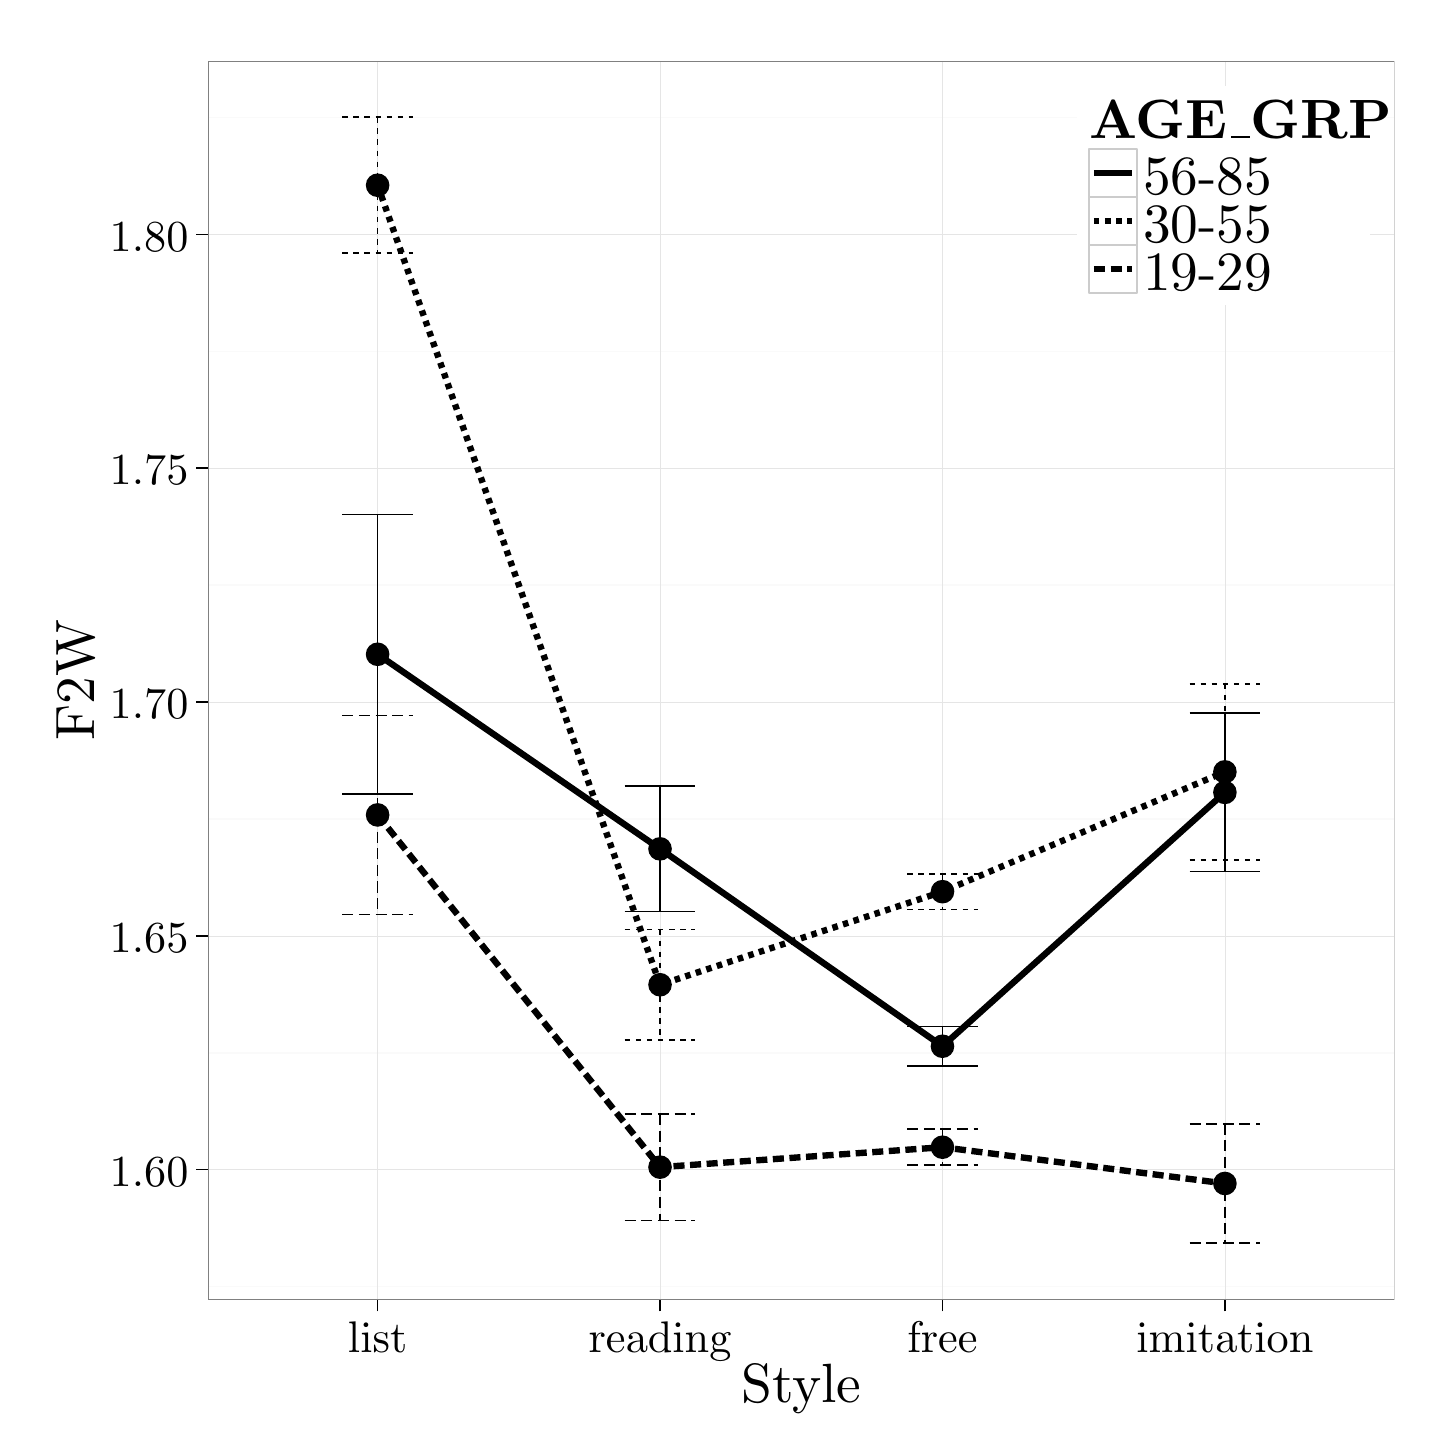
\begin{tikzpicture}[x=1pt,y=1pt]
\definecolor{fillColor}{RGB}{255,255,255}
\path[use as bounding box,fill=fillColor,fill opacity=0.00] (0,0) rectangle (505.89,505.89);
\begin{scope}
\path[clip] (  0.00,  0.00) rectangle (505.89,505.89);
\definecolor{drawColor}{RGB}{255,255,255}
\definecolor{fillColor}{RGB}{255,255,255}

\path[draw=drawColor,line width= 0.6pt,line join=round,line cap=round,fill=fillColor] (  0.00, -0.00) rectangle (505.89,505.89);
\end{scope}
\begin{scope}
\path[clip] ( 65.21, 46.31) rectangle (493.85,493.84);
\definecolor{fillColor}{RGB}{255,255,255}

\path[fill=fillColor] ( 65.21, 46.31) rectangle (493.85,493.84);
\definecolor{drawColor}{gray}{0.98}

\path[draw=drawColor,line width= 0.6pt,line join=round] ( 65.21, 51.03) --
	(493.85, 51.03);

\path[draw=drawColor,line width= 0.6pt,line join=round] ( 65.21,135.50) --
	(493.85,135.50);

\path[draw=drawColor,line width= 0.6pt,line join=round] ( 65.21,219.97) --
	(493.85,219.97);

\path[draw=drawColor,line width= 0.6pt,line join=round] ( 65.21,304.44) --
	(493.85,304.44);

\path[draw=drawColor,line width= 0.6pt,line join=round] ( 65.21,388.91) --
	(493.85,388.91);

\path[draw=drawColor,line width= 0.6pt,line join=round] ( 65.21,473.38) --
	(493.85,473.38);
\definecolor{drawColor}{gray}{0.90}

\path[draw=drawColor,line width= 0.2pt,line join=round] ( 65.21, 93.27) --
	(493.85, 93.27);

\path[draw=drawColor,line width= 0.2pt,line join=round] ( 65.21,177.74) --
	(493.85,177.74);

\path[draw=drawColor,line width= 0.2pt,line join=round] ( 65.21,262.20) --
	(493.85,262.20);

\path[draw=drawColor,line width= 0.2pt,line join=round] ( 65.21,346.67) --
	(493.85,346.67);

\path[draw=drawColor,line width= 0.2pt,line join=round] ( 65.21,431.14) --
	(493.85,431.14);

\path[draw=drawColor,line width= 0.2pt,line join=round] (126.45, 46.31) --
	(126.45,493.84);

\path[draw=drawColor,line width= 0.2pt,line join=round] (228.50, 46.31) --
	(228.50,493.84);

\path[draw=drawColor,line width= 0.2pt,line join=round] (330.56, 46.31) --
	(330.56,493.84);

\path[draw=drawColor,line width= 0.2pt,line join=round] (432.61, 46.31) --
	(432.61,493.84);
\definecolor{fillColor}{RGB}{0,0,0}

\path[fill=fillColor] (126.45,279.46) circle (  4.27);

\path[fill=fillColor] (126.45,448.95) circle (  4.27);

\path[fill=fillColor] (126.45,221.41) circle (  4.27);

\path[fill=fillColor] (228.50,209.15) circle (  4.27);

\path[fill=fillColor] (228.50,160.05) circle (  4.27);

\path[fill=fillColor] (228.50, 94.14) circle (  4.27);

\path[fill=fillColor] (330.56,137.83) circle (  4.27);

\path[fill=fillColor] (330.56,193.68) circle (  4.27);

\path[fill=fillColor] (330.56,101.34) circle (  4.27);

\path[fill=fillColor] (432.61,229.56) circle (  4.27);

\path[fill=fillColor] (432.61,236.98) circle (  4.27);

\path[fill=fillColor] (432.61, 88.24) circle (  4.27);
\definecolor{drawColor}{RGB}{0,0,0}

\path[draw=drawColor,line width= 2.3pt,line join=round] (126.45,279.46) --
	(228.50,209.15) --
	(330.56,137.83) --
	(432.61,229.56);

\path[draw=drawColor,line width= 2.3pt,dash pattern=on 2pt off 2pt ,line join=round] (126.45,448.95) --
	(228.50,160.05) --
	(330.56,193.68) --
	(432.61,236.98);

\path[draw=drawColor,line width= 2.3pt,dash pattern=on 4pt off 2pt ,line join=round] (126.45,221.41) --
	(228.50, 94.14) --
	(330.56,101.34) --
	(432.61, 88.24);

\path[draw=drawColor,line width= 0.6pt,line join=round] (113.69,330.03) --
	(139.20,330.03);

\path[draw=drawColor,line width= 0.6pt,line join=round] (126.45,330.03) --
	(126.45,228.90);

\path[draw=drawColor,line width= 0.6pt,line join=round] (113.69,228.90) --
	(139.20,228.90);

\path[draw=drawColor,line width= 0.6pt,line join=round] (215.75,231.83) --
	(241.26,231.83);

\path[draw=drawColor,line width= 0.6pt,line join=round] (228.50,231.83) --
	(228.50,186.47);

\path[draw=drawColor,line width= 0.6pt,line join=round] (215.75,186.47) --
	(241.26,186.47);

\path[draw=drawColor,line width= 0.6pt,line join=round] (317.80,145.01) --
	(343.31,145.01);

\path[draw=drawColor,line width= 0.6pt,line join=round] (330.56,145.01) --
	(330.56,130.65);

\path[draw=drawColor,line width= 0.6pt,line join=round] (317.80,130.65) --
	(343.31,130.65);

\path[draw=drawColor,line width= 0.6pt,line join=round] (419.86,258.17) --
	(445.37,258.17);

\path[draw=drawColor,line width= 0.6pt,line join=round] (432.61,258.17) --
	(432.61,200.95);

\path[draw=drawColor,line width= 0.6pt,line join=round] (419.86,200.95) --
	(445.37,200.95);

\path[draw=drawColor,line width= 0.6pt,dash pattern=on 2pt off 2pt ,line join=round] (113.69,473.50) --
	(139.20,473.50);

\path[draw=drawColor,line width= 0.6pt,dash pattern=on 2pt off 2pt ,line join=round] (126.45,473.50) --
	(126.45,424.39);

\path[draw=drawColor,line width= 0.6pt,dash pattern=on 2pt off 2pt ,line join=round] (113.69,424.39) --
	(139.20,424.39);

\path[draw=drawColor,line width= 0.6pt,dash pattern=on 2pt off 2pt ,line join=round] (215.75,179.98) --
	(241.26,179.98);

\path[draw=drawColor,line width= 0.6pt,dash pattern=on 2pt off 2pt ,line join=round] (228.50,179.98) --
	(228.50,140.12);

\path[draw=drawColor,line width= 0.6pt,dash pattern=on 2pt off 2pt ,line join=round] (215.75,140.12) --
	(241.26,140.12);

\path[draw=drawColor,line width= 0.6pt,dash pattern=on 2pt off 2pt ,line join=round] (317.80,200.07) --
	(343.31,200.07);

\path[draw=drawColor,line width= 0.6pt,dash pattern=on 2pt off 2pt ,line join=round] (330.56,200.07) --
	(330.56,187.29);

\path[draw=drawColor,line width= 0.6pt,dash pattern=on 2pt off 2pt ,line join=round] (317.80,187.29) --
	(343.31,187.29);

\path[draw=drawColor,line width= 0.6pt,dash pattern=on 2pt off 2pt ,line join=round] (419.86,268.82) --
	(445.37,268.82);

\path[draw=drawColor,line width= 0.6pt,dash pattern=on 2pt off 2pt ,line join=round] (432.61,268.82) --
	(432.61,205.14);

\path[draw=drawColor,line width= 0.6pt,dash pattern=on 2pt off 2pt ,line join=round] (419.86,205.14) --
	(445.37,205.14);

\path[draw=drawColor,line width= 0.6pt,dash pattern=on 4pt off 2pt ,line join=round] (113.69,257.38) --
	(139.20,257.38);

\path[draw=drawColor,line width= 0.6pt,dash pattern=on 4pt off 2pt ,line join=round] (126.45,257.38) --
	(126.45,185.44);

\path[draw=drawColor,line width= 0.6pt,dash pattern=on 4pt off 2pt ,line join=round] (113.69,185.44) --
	(139.20,185.44);

\path[draw=drawColor,line width= 0.6pt,dash pattern=on 4pt off 2pt ,line join=round] (215.75,113.38) --
	(241.26,113.38);

\path[draw=drawColor,line width= 0.6pt,dash pattern=on 4pt off 2pt ,line join=round] (228.50,113.38) --
	(228.50, 74.91);

\path[draw=drawColor,line width= 0.6pt,dash pattern=on 4pt off 2pt ,line join=round] (215.75, 74.91) --
	(241.26, 74.91);

\path[draw=drawColor,line width= 0.6pt,dash pattern=on 4pt off 2pt ,line join=round] (317.80,107.87) --
	(343.31,107.87);

\path[draw=drawColor,line width= 0.6pt,dash pattern=on 4pt off 2pt ,line join=round] (330.56,107.87) --
	(330.56, 94.82);

\path[draw=drawColor,line width= 0.6pt,dash pattern=on 4pt off 2pt ,line join=round] (317.80, 94.82) --
	(343.31, 94.82);

\path[draw=drawColor,line width= 0.6pt,dash pattern=on 4pt off 2pt ,line join=round] (419.86,109.84) --
	(445.37,109.84);

\path[draw=drawColor,line width= 0.6pt,dash pattern=on 4pt off 2pt ,line join=round] (432.61,109.84) --
	(432.61, 66.65);

\path[draw=drawColor,line width= 0.6pt,dash pattern=on 4pt off 2pt ,line join=round] (419.86, 66.65) --
	(445.37, 66.65);
\definecolor{drawColor}{gray}{0.50}

\path[draw=drawColor,line width= 0.6pt,line join=round,line cap=round] ( 65.21, 46.31) rectangle (493.85,493.84);
\end{scope}
\begin{scope}
\path[clip] (  0.00,  0.00) rectangle (505.89,505.89);
\definecolor{drawColor}{RGB}{0,0,0}

\node[text=drawColor,anchor=base east,inner sep=0pt, outer sep=0pt, scale=  1.60] at ( 58.10, 87.23) {1.60};

\node[text=drawColor,anchor=base east,inner sep=0pt, outer sep=0pt, scale=  1.60] at ( 58.10,171.70) {1.65};

\node[text=drawColor,anchor=base east,inner sep=0pt, outer sep=0pt, scale=  1.60] at ( 58.10,256.17) {1.70};

\node[text=drawColor,anchor=base east,inner sep=0pt, outer sep=0pt, scale=  1.60] at ( 58.10,340.64) {1.75};

\node[text=drawColor,anchor=base east,inner sep=0pt, outer sep=0pt, scale=  1.60] at ( 58.10,425.11) {1.80};
\end{scope}
\begin{scope}
\path[clip] (  0.00,  0.00) rectangle (505.89,505.89);
\definecolor{drawColor}{RGB}{0,0,0}

\path[draw=drawColor,line width= 0.6pt,line join=round] ( 60.95, 93.27) --
	( 65.21, 93.27);

\path[draw=drawColor,line width= 0.6pt,line join=round] ( 60.95,177.74) --
	( 65.21,177.74);

\path[draw=drawColor,line width= 0.6pt,line join=round] ( 60.95,262.20) --
	( 65.21,262.20);

\path[draw=drawColor,line width= 0.6pt,line join=round] ( 60.95,346.67) --
	( 65.21,346.67);

\path[draw=drawColor,line width= 0.6pt,line join=round] ( 60.95,431.14) --
	( 65.21,431.14);
\end{scope}
\begin{scope}
\path[clip] (  0.00,  0.00) rectangle (505.89,505.89);
\definecolor{drawColor}{RGB}{0,0,0}

\path[draw=drawColor,line width= 0.6pt,line join=round] (126.45, 42.04) --
	(126.45, 46.31);

\path[draw=drawColor,line width= 0.6pt,line join=round] (228.50, 42.04) --
	(228.50, 46.31);

\path[draw=drawColor,line width= 0.6pt,line join=round] (330.56, 42.04) --
	(330.56, 46.31);

\path[draw=drawColor,line width= 0.6pt,line join=round] (432.61, 42.04) --
	(432.61, 46.31);
\end{scope}
\begin{scope}
\path[clip] (  0.00,  0.00) rectangle (505.89,505.89);
\definecolor{drawColor}{RGB}{0,0,0}

\node[text=drawColor,anchor=base,inner sep=0pt, outer sep=0pt, scale=  1.60] at (126.45, 27.13) {list};

\node[text=drawColor,anchor=base,inner sep=0pt, outer sep=0pt, scale=  1.60] at (228.50, 27.13) {reading};

\node[text=drawColor,anchor=base,inner sep=0pt, outer sep=0pt, scale=  1.60] at (330.56, 27.13) {free};

\node[text=drawColor,anchor=base,inner sep=0pt, outer sep=0pt, scale=  1.60] at (432.61, 27.13) {imitation};
\end{scope}
\begin{scope}
\path[clip] (  0.00,  0.00) rectangle (505.89,505.89);
\definecolor{drawColor}{RGB}{0,0,0}

\node[text=drawColor,anchor=base,inner sep=0pt, outer sep=0pt, scale=  2.00] at (279.53,  9.03) {Style};
\end{scope}
\begin{scope}
\path[clip] (  0.00,  0.00) rectangle (505.89,505.89);
\definecolor{drawColor}{RGB}{0,0,0}

\node[text=drawColor,rotate= 90.00,anchor=base,inner sep=0pt, outer sep=0pt, scale=  2.00] at ( 24.12,270.08) {F2W};
\end{scope}
\begin{scope}
\path[clip] (  0.00,  0.00) rectangle (505.89,505.89);
\definecolor{fillColor}{RGB}{255,255,255}

\path[fill=fillColor] (379.28,405.66) rectangle (484.98,484.98);
\end{scope}
\begin{scope}
\path[clip] (  0.00,  0.00) rectangle (505.89,505.89);
\definecolor{drawColor}{RGB}{0,0,0}

\node[text=drawColor,anchor=base west,inner sep=0pt, outer sep=0pt, scale=  2.00] at (383.55,465.96) {\bfseries AGE{\_{}}GRP};
\end{scope}
\begin{scope}
\path[clip] (  0.00,  0.00) rectangle (505.89,505.89);
\definecolor{drawColor}{gray}{0.80}
\definecolor{fillColor}{RGB}{255,255,255}

\path[draw=drawColor,line width= 0.6pt,line join=round,line cap=round,fill=fillColor] (383.55,444.61) rectangle (400.89,461.96);
\end{scope}
\begin{scope}
\path[clip] (  0.00,  0.00) rectangle (505.89,505.89);
\definecolor{drawColor}{RGB}{0,0,0}

\path[draw=drawColor,line width= 2.3pt,line join=round] (385.28,453.29) -- (399.16,453.29);
\end{scope}
\begin{scope}
\path[clip] (  0.00,  0.00) rectangle (505.89,505.89);
\definecolor{drawColor}{RGB}{0,0,0}

\path[draw=drawColor,line width= 0.6pt,line join=round] (385.28,453.29) -- (399.16,453.29);
\end{scope}
\begin{scope}
\path[clip] (  0.00,  0.00) rectangle (505.89,505.89);
\definecolor{drawColor}{gray}{0.80}
\definecolor{fillColor}{RGB}{255,255,255}

\path[draw=drawColor,line width= 0.6pt,line join=round,line cap=round,fill=fillColor] (383.55,427.27) rectangle (400.89,444.61);
\end{scope}
\begin{scope}
\path[clip] (  0.00,  0.00) rectangle (505.89,505.89);
\definecolor{drawColor}{RGB}{0,0,0}

\path[draw=drawColor,line width= 2.3pt,dash pattern=on 2pt off 2pt ,line join=round] (385.28,435.94) -- (399.16,435.94);
\end{scope}
\begin{scope}
\path[clip] (  0.00,  0.00) rectangle (505.89,505.89);
\definecolor{drawColor}{RGB}{0,0,0}

\path[draw=drawColor,line width= 0.6pt,dash pattern=on 2pt off 2pt ,line join=round] (385.28,435.94) -- (399.16,435.94);
\end{scope}
\begin{scope}
\path[clip] (  0.00,  0.00) rectangle (505.89,505.89);
\definecolor{drawColor}{gray}{0.80}
\definecolor{fillColor}{RGB}{255,255,255}

\path[draw=drawColor,line width= 0.6pt,line join=round,line cap=round,fill=fillColor] (383.55,409.92) rectangle (400.89,427.27);
\end{scope}
\begin{scope}
\path[clip] (  0.00,  0.00) rectangle (505.89,505.89);
\definecolor{drawColor}{RGB}{0,0,0}

\path[draw=drawColor,line width= 2.3pt,dash pattern=on 4pt off 2pt ,line join=round] (385.28,418.60) -- (399.16,418.60);
\end{scope}
\begin{scope}
\path[clip] (  0.00,  0.00) rectangle (505.89,505.89);
\definecolor{drawColor}{RGB}{0,0,0}

\path[draw=drawColor,line width= 0.6pt,dash pattern=on 4pt off 2pt ,line join=round] (385.28,418.60) -- (399.16,418.60);
\end{scope}
\begin{scope}
\path[clip] (  0.00,  0.00) rectangle (505.89,505.89);
\definecolor{drawColor}{RGB}{0,0,0}

\node[text=drawColor,anchor=base west,inner sep=0pt, outer sep=0pt, scale=  2.00] at (403.06,445.75) {56-85};
\end{scope}
\begin{scope}
\path[clip] (  0.00,  0.00) rectangle (505.89,505.89);
\definecolor{drawColor}{RGB}{0,0,0}

\node[text=drawColor,anchor=base west,inner sep=0pt, outer sep=0pt, scale=  2.00] at (403.06,428.40) {30-55};
\end{scope}
\begin{scope}
\path[clip] (  0.00,  0.00) rectangle (505.89,505.89);
\definecolor{drawColor}{RGB}{0,0,0}

\node[text=drawColor,anchor=base west,inner sep=0pt, outer sep=0pt, scale=  2.00] at (403.06,411.06) {19-29};
\end{scope}
\end{tikzpicture}
} 
	\caption{happ\textsc{y} (F2) by age and style}
	\label{fig.line.f2w.happy.tot}
\end{figure}

Before concluding this section, we will have a closer look at style and its (lacking) relation to age.
I am aware of the fact that the linear mixed-effects regression did not find a significant interaction of these two predictors.
Just as for the F1 dimension of happ\textsc{y} I will print and describe the relevant plot all the same, because,
\begin{inparaenum}[(a)]
	\item in this particular case, it visualises the impact of style almost as well as a plot that does not include age at all, and
	\item both plots will later serve as points of reference for variables where there \emph{is} a significant interaction.
\end{inparaenum}
Figure \ref{fig.line.f2w.happy.tot} is identical in design to Figure \ref{fig.line.f1w.happy.tot}: style is marked on the x-, and F2 on the y-axis.
Age group is coded by line type, and the whiskers visualise standard deviations.

For all three age groups, there is a sharp drop from the word list to reading and the other two styles (with the exception of `imitation\is{accent performance}' in the old group, which looks as if it might not be significantly different from the word list values in the same age group).
This echoes what has been found for F1 of happ\textsc{y}, and could, at least in parts, also be explained the same way: \isi{vowel duration} is considerably higher when participants read out a word list (and also very similar in the other three registers; cf. Table \ref{tab.dur.style.happy}), so the high values in this style are probably less to do with \isi{style shifting} than with mere phonetic factors (although this does not explain why the difference seems to be particularly extreme for the middle age group).

One might be tempted to see some regularity in this graph (comparable to the u-shape in Figure \ref{fig.line.f1w.happy.tot}), but the evidence is inconclusive.
For the oldest speakers (where free speech marks the low point, and happ\textsc{y} is more advanced both during reading and accent perform\is{accent performance}ance, which do not seem to differ significantly), a two-norms-approach might actually work pretty well: tense /i/ seems to be the target both in particularly local and particularly standard, or careful, speech.
In the middle group, however, the three registers `reading', `free', and `imitation\is{accent performance}' do not only apparently all differ significantly from one another (the standard deviations do not overlap), but happ\textsc{y} is also more advanced in spontaneous speech than it is while reading a text --- a fact, which does not go together very well with the assumption that a more formal register should pull realisations towards the tense standard, relative to a more relaxed (and therefore more central) starting point in spontaneous speech.
For the youngest speakers in the sample, finally, this interpretation is completely out of the question.
In this group, happ\textsc{y} realisations are virtually identical with respect to F2 in reading, free speech, and accent perform\is{accent performance}ance (standard deviations for these styles completely overlap).
As far as the front-back dimension of happ\textsc{y} is concerned, the youngest speakers that were interviewed for this study are not only, once again, the least Scouse (the dashed line is below the other two in all styles), but they also show the least aware\is{awareness}ness (\emph{if} there is any to start with) of this feature as measured by \isi{style shifting}.

\subsection{Synthesis and Pillai scores (happ\textsc{y})}
\label{sec.prod.res.vow.happy.pil}

\subsubsection{Overview}

Moving away from aware\is{awareness}ness for a moment but keeping the focus on age, we will now zoom out a bit further and consider F1 and F2 measurements of happ\textsc{y} together.
The test variable happ\textsc{y} will also be contrasted with \textsc{fleece}.
This might provide a first hint as to whether just happ\textsc{y} is changing in the younger generation, or whether other high front vowels are moving in the same (or another) direction as well.
It should be noted, though, that \textsc{fleece} vowels were only measured in the reading and word list sections of the interviews (cf. \ref{sec.prod_method.vow}).
For the graphs reported on the following pages, the dataset of happ\textsc{y} observations was therefore also reduced to the ones derived from reading and word list realisations to make sure like is compared with like.

\begin{figure}[h!]
	\centering
	\begin{subfigure}{.49\textwidth}
		\centering
			\definecolor{shadecolor}{rgb}{0.969, 0.969, 0.969}
			\resizebox{\linewidth}{!}{% Created by tikzDevice version 0.8.1 on 2016-02-09 02:14:14
% !TEX encoding = UTF-8 Unicode
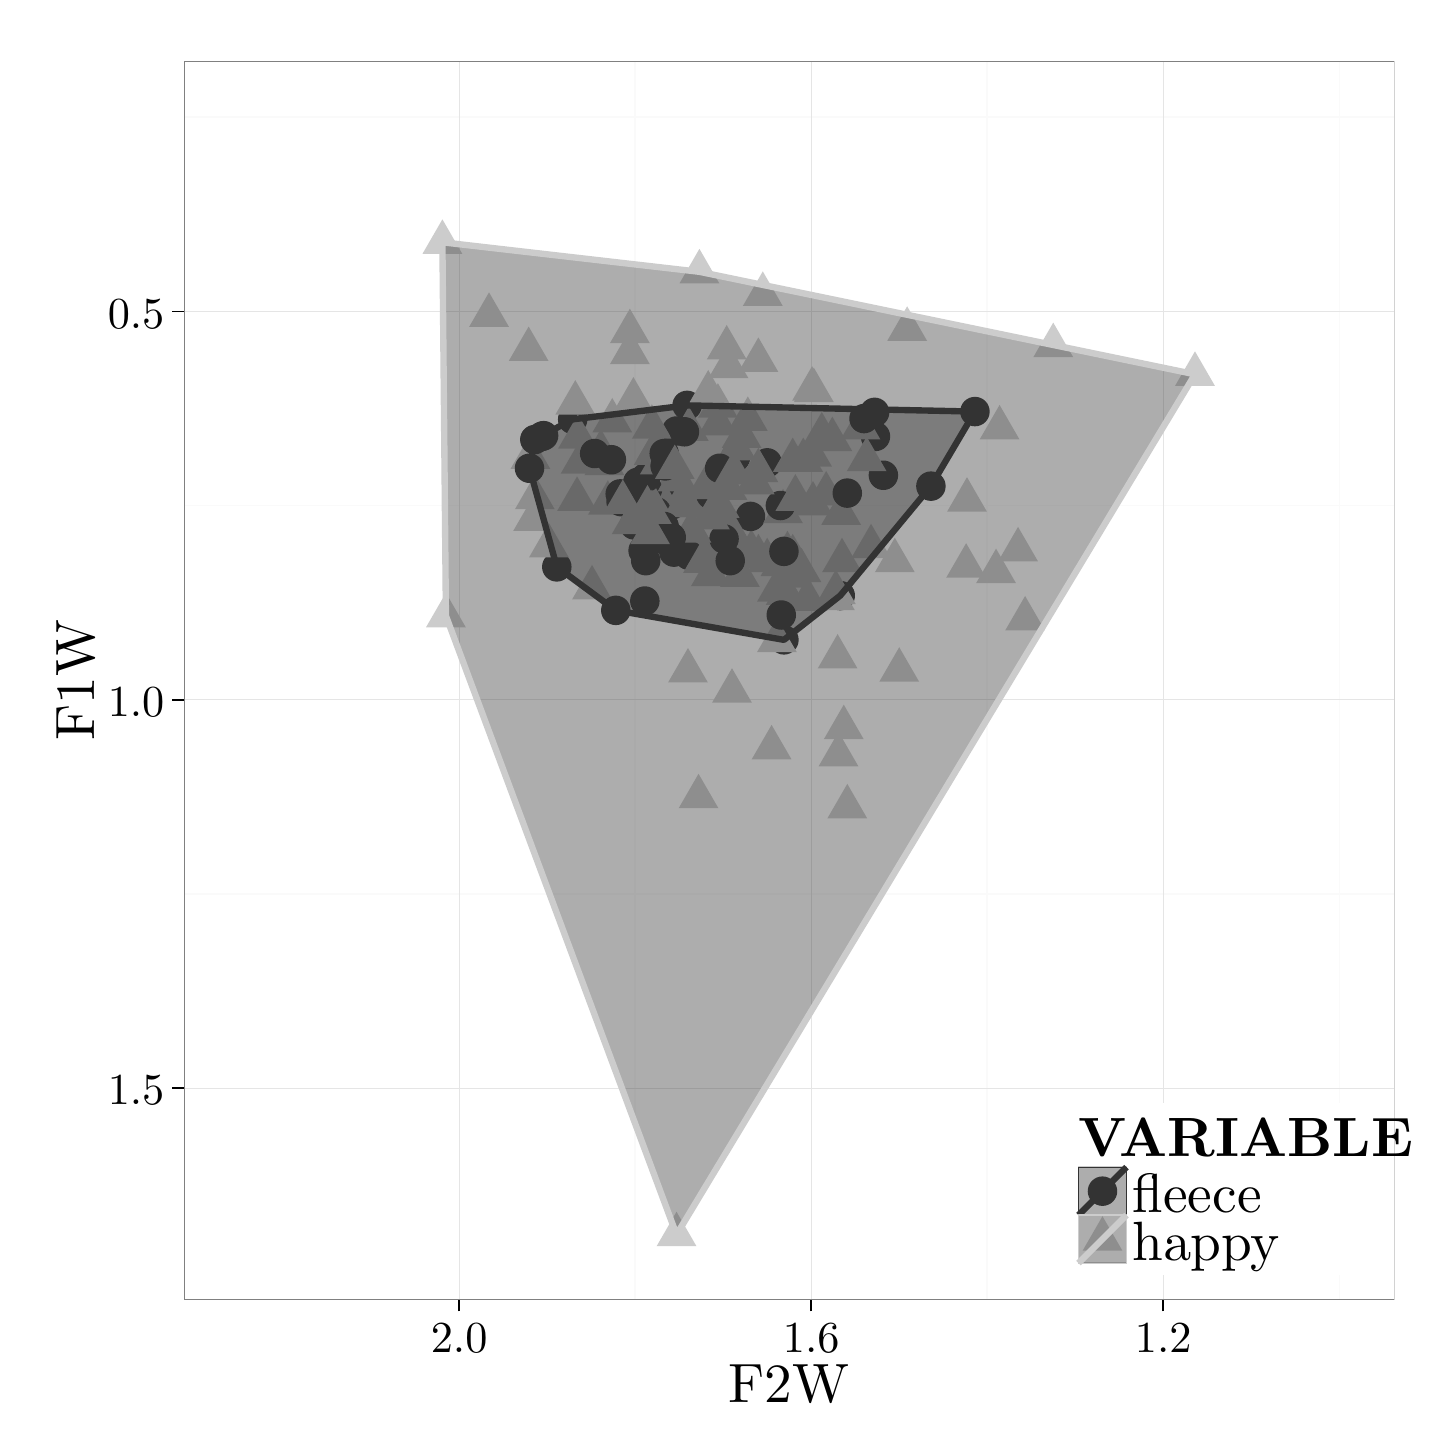
\begin{tikzpicture}[x=1pt,y=1pt]
\definecolor{fillColor}{RGB}{255,255,255}
\path[use as bounding box,fill=fillColor,fill opacity=0.00] (0,0) rectangle (505.89,505.89);
\begin{scope}
\path[clip] (  0.00,  0.00) rectangle (505.89,505.89);
\definecolor{drawColor}{RGB}{255,255,255}
\definecolor{fillColor}{RGB}{255,255,255}

\path[draw=drawColor,line width= 0.6pt,line join=round,line cap=round,fill=fillColor] (  0.00, -0.00) rectangle (505.89,505.89);
\end{scope}
\begin{scope}
\path[clip] ( 56.50, 46.31) rectangle (493.85,493.84);
\definecolor{fillColor}{RGB}{255,255,255}

\path[fill=fillColor] ( 56.50, 46.31) rectangle (493.85,493.84);
\definecolor{drawColor}{gray}{0.98}

\path[draw=drawColor,line width= 0.6pt,line join=round] ( 56.50,473.50) --
	(493.85,473.50);

\path[draw=drawColor,line width= 0.6pt,line join=round] ( 56.50,333.21) --
	(493.85,333.21);

\path[draw=drawColor,line width= 0.6pt,line join=round] ( 56.50,192.91) --
	(493.85,192.91);

\path[draw=drawColor,line width= 0.6pt,line join=round] (473.97, 46.31) --
	(473.97,493.84);

\path[draw=drawColor,line width= 0.6pt,line join=round] (346.74, 46.31) --
	(346.74,493.84);

\path[draw=drawColor,line width= 0.6pt,line join=round] (219.51, 46.31) --
	(219.51,493.84);
\definecolor{drawColor}{gray}{0.90}

\path[draw=drawColor,line width= 0.2pt,line join=round] ( 56.50,403.36) --
	(493.85,403.36);

\path[draw=drawColor,line width= 0.2pt,line join=round] ( 56.50,263.06) --
	(493.85,263.06);

\path[draw=drawColor,line width= 0.2pt,line join=round] ( 56.50,122.77) --
	(493.85,122.77);

\path[draw=drawColor,line width= 0.2pt,line join=round] (410.35, 46.31) --
	(410.35,493.84);

\path[draw=drawColor,line width= 0.2pt,line join=round] (283.13, 46.31) --
	(283.13,493.84);

\path[draw=drawColor,line width= 0.2pt,line join=round] (155.90, 46.31) --
	(155.90,493.84);
\definecolor{fillColor}{gray}{0.80}

\path[fill=fillColor] (261.50,324.67) --
	(268.68,312.23) --
	(254.31,312.23) --
	cycle;
\definecolor{fillColor}{gray}{0.20}

\path[fill=fillColor] (261.18,329.28) circle (  5.33);

\path[fill=fillColor] (232.87,333.49) circle (  5.33);
\definecolor{fillColor}{gray}{0.80}

\path[fill=fillColor] (227.15,361.99) --
	(234.33,349.54) --
	(219.96,349.54) --
	cycle;
\definecolor{fillColor}{gray}{0.20}

\path[fill=fillColor] (219.19,326.19) circle (  5.33);
\definecolor{fillColor}{gray}{0.80}

\path[fill=fillColor] (293.94,338.70) --
	(301.13,326.25) --
	(286.76,326.25) --
	cycle;
\definecolor{fillColor}{gray}{0.20}

\path[fill=fillColor] (220.47,341.63) circle (  5.33);
\definecolor{fillColor}{gray}{0.80}

\path[fill=fillColor] (270.72,310.92) --
	(277.91,298.48) --
	(263.54,298.48) --
	cycle;

\path[fill=fillColor] (279.63,317.94) --
	(286.81,305.49) --
	(272.44,305.49) --
	cycle;

\path[fill=fillColor] (209.65,342.35) --
	(216.84,329.90) --
	(202.47,329.90) --
	cycle;

\path[fill=fillColor] (288.53,345.71) --
	(295.72,333.27) --
	(281.35,333.27) --
	cycle;
\definecolor{fillColor}{gray}{0.20}

\path[fill=fillColor] (214.42,334.61) circle (  5.33);

\path[fill=fillColor] (196.93,364.35) circle (  5.33);

\path[fill=fillColor] (269.45,313.85) circle (  5.33);
\definecolor{fillColor}{gray}{0.80}

\path[fill=fillColor] (252.59,398.46) --
	(259.78,386.02) --
	(245.41,386.02) --
	cycle;

\path[fill=fillColor] (208.38,356.66) --
	(215.57,344.21) --
	(201.20,344.21) --
	cycle;
\definecolor{fillColor}{gray}{0.20}

\path[fill=fillColor] (267.22,348.64) circle (  5.33);
\definecolor{fillColor}{gray}{0.80}

\path[fill=fillColor] (255.45,329.72) --
	(262.64,317.28) --
	(248.27,317.28) --
	cycle;
\definecolor{fillColor}{gray}{0.20}

\path[fill=fillColor] (238.28,369.40) circle (  5.33);
\definecolor{fillColor}{gray}{0.80}

\path[fill=fillColor] (253.55,332.53) --
	(260.73,320.08) --
	(246.36,320.08) --
	cycle;
\definecolor{fillColor}{gray}{0.20}

\path[fill=fillColor] (223.33,313.29) circle (  5.33);
\definecolor{fillColor}{gray}{0.80}

\path[fill=fillColor] (281.85,307.55) --
	(289.04,295.11) --
	(274.67,295.11) --
	cycle;

\path[fill=fillColor] (238.91,369.00) --
	(246.10,356.56) --
	(231.73,356.56) --
	cycle;

\path[fill=fillColor] (294.26,321.58) --
	(301.44,309.14) --
	(287.07,309.14) --
	cycle;

\path[fill=fillColor] (183.25,344.31) --
	(190.44,331.87) --
	(176.07,331.87) --
	cycle;

\path[fill=fillColor] (221.10,339.26) --
	(228.29,326.82) --
	(213.92,326.82) --
	cycle;

\path[fill=fillColor] (149.86,436.62) --
	(157.04,424.18) --
	(142.67,424.18) --
	cycle;
\definecolor{fillColor}{gray}{0.20}

\path[fill=fillColor] (234.46,360.14) circle (  5.33);
\definecolor{fillColor}{gray}{0.80}

\path[fill=fillColor] (246.87,316.53) --
	(254.05,304.09) --
	(239.68,304.09) --
	cycle;

\path[fill=fillColor] (242.10,341.50) --
	(249.28,329.06) --
	(234.91,329.06) --
	cycle;

\path[fill=fillColor] (264.04,322.99) --
	(271.23,310.54) --
	(256.86,310.54) --
	cycle;

\path[fill=fillColor] (211.24,372.09) --
	(218.43,359.64) --
	(204.06,359.64) --
	cycle;

\path[fill=fillColor] (181.66,358.90) --
	(188.85,346.46) --
	(174.48,346.46) --
	cycle;

\path[fill=fillColor] (245.91,382.19) --
	(253.10,369.75) --
	(238.73,369.75) --
	cycle;

\path[fill=fillColor] (198.84,366.20) --
	(206.02,353.75) --
	(191.65,353.75) --
	cycle;

\path[fill=fillColor] (254.18,356.38) --
	(261.37,343.93) --
	(247.00,343.93) --
	cycle;

\path[fill=fillColor] (166.71,410.25) --
	(173.90,397.80) --
	(159.53,397.80) --
	cycle;

\path[fill=fillColor] (264.04,393.97) --
	(271.23,381.53) --
	(256.86,381.53) --
	cycle;

\path[fill=fillColor] (229.37,342.91) --
	(236.56,330.46) --
	(222.19,330.46) --
	cycle;
\definecolor{fillColor}{gray}{0.20}

\path[fill=fillColor] (293.62,300.66) circle (  5.33);
\definecolor{fillColor}{gray}{0.80}

\path[fill=fillColor] (181.03,397.90) --
	(188.21,385.46) --
	(173.84,385.46) --
	cycle;

\path[fill=fillColor] (253.23,391.73) --
	(260.41,379.29) --
	(246.04,379.29) --
	cycle;

\path[fill=fillColor] (317.80,405.20) --
	(324.98,392.75) --
	(310.61,392.75) --
	cycle;
\definecolor{fillColor}{gray}{0.20}

\path[fill=fillColor] (255.77,350.60) circle (  5.33);
\definecolor{fillColor}{gray}{0.80}

\path[fill=fillColor] (273.90,309.80) --
	(281.09,297.35) --
	(266.72,297.35) --
	cycle;
\definecolor{fillColor}{gray}{0.20}

\path[fill=fillColor] (223.01,298.70) circle (  5.33);

\path[fill=fillColor] (306.03,366.88) circle (  5.33);
\definecolor{fillColor}{gray}{0.80}

\path[fill=fillColor] (313.34,321.58) --
	(320.53,309.14) --
	(306.16,309.14) --
	cycle;
\definecolor{fillColor}{gray}{0.20}

\path[fill=fillColor] (181.34,346.68) circle (  5.33);
\definecolor{fillColor}{gray}{0.80}

\path[fill=fillColor] (291.71,307.83) --
	(298.90,295.39) --
	(284.53,295.39) --
	cycle;
\definecolor{fillColor}{gray}{0.20}

\path[fill=fillColor] (185.80,358.18) circle (  5.33);
\definecolor{fillColor}{gray}{0.80}

\path[fill=fillColor] (294.89,261.26) --
	(302.08,248.81) --
	(287.71,248.81) --
	cycle;

\path[fill=fillColor] (268.81,253.96) --
	(276.00,241.52) --
	(261.63,241.52) --
	cycle;

\path[fill=fillColor] (349.92,317.65) --
	(357.10,305.21) --
	(342.74,305.21) --
	cycle;

\path[fill=fillColor] (272.95,339.26) --
	(280.13,326.82) --
	(265.76,326.82) --
	cycle;
\definecolor{fillColor}{gray}{0.20}

\path[fill=fillColor] (183.25,357.06) circle (  5.33);

\path[fill=fillColor] (223.97,339.10) circle (  5.33);

\path[fill=fillColor] (273.27,284.67) circle (  5.33);
\definecolor{fillColor}{gray}{0.80}

\path[fill=fillColor] (235.42,341.50) --
	(242.60,329.06) --
	(228.23,329.06) --
	cycle;
\definecolor{fillColor}{gray}{0.20}

\path[fill=fillColor] (342.29,367.16) circle (  5.33);
\definecolor{fillColor}{gray}{0.80}

\path[fill=fillColor] (314.93,282.02) --
	(322.12,269.58) --
	(307.75,269.58) --
	cycle;

\path[fill=fillColor] (292.03,310.08) --
	(299.22,297.63) --
	(284.85,297.63) --
	cycle;
\definecolor{fillColor}{gray}{0.20}

\path[fill=fillColor] (191.20,311.04) circle (  5.33);
\definecolor{fillColor}{gray}{0.80}

\path[fill=fillColor] (276.45,315.97) --
	(283.63,303.53) --
	(269.26,303.53) --
	cycle;
\definecolor{fillColor}{gray}{0.20}

\path[fill=fillColor] (227.15,330.96) circle (  5.33);
\definecolor{fillColor}{gray}{0.80}

\path[fill=fillColor] (254.50,274.44) --
	(261.68,262.00) --
	(247.32,262.00) --
	cycle;

\path[fill=fillColor] (225.87,341.50) --
	(233.06,329.06) --
	(218.69,329.06) --
	cycle;

\path[fill=fillColor] (243.37,326.35) --
	(250.55,313.91) --
	(236.18,313.91) --
	cycle;

\path[fill=fillColor] (151.13,301.66) --
	(158.31,289.22) --
	(143.94,289.22) --
	cycle;
\definecolor{fillColor}{gray}{0.20}

\path[fill=fillColor] (214.11,337.42) circle (  5.33);
\definecolor{fillColor}{gray}{0.80}

\path[fill=fillColor] (296.17,232.64) --
	(303.35,220.19) --
	(288.98,220.19) --
	cycle;

\path[fill=fillColor] (339.11,319.62) --
	(346.29,307.17) --
	(331.92,307.17) --
	cycle;

\path[fill=fillColor] (234.46, 78.03) --
	(241.65, 65.59) --
	(227.28, 65.59) --
	cycle;

\path[fill=fillColor] (277.40,344.59) --
	(284.59,332.15) --
	(270.22,332.15) --
	cycle;

\path[fill=fillColor] (203.93,311.76) --
	(211.11,299.32) --
	(196.74,299.32) --
	cycle;

\path[fill=fillColor] (360.42,300.54) --
	(367.60,288.09) --
	(353.23,288.09) --
	cycle;

\path[fill=fillColor] (274.54,324.11) --
	(281.72,311.66) --
	(267.35,311.66) --
	cycle;

\path[fill=fillColor] (278.67,318.78) --
	(285.86,306.33) --
	(271.49,306.33) --
	cycle;

\path[fill=fillColor] (267.22,321.58) --
	(274.41,309.14) --
	(260.04,309.14) --
	cycle;

\path[fill=fillColor] (256.09,361.99) --
	(263.28,349.54) --
	(248.91,349.54) --
	cycle;

\path[fill=fillColor] (270.72,292.68) --
	(277.91,280.24) --
	(263.54,280.24) --
	cycle;

\path[fill=fillColor] (207.11,360.87) --
	(214.29,348.42) --
	(199.92,348.42) --
	cycle;

\path[fill=fillColor] (182.62,336.45) --
	(189.80,324.01) --
	(175.43,324.01) --
	cycle;
\definecolor{fillColor}{gray}{0.20}

\path[fill=fillColor] (272.31,293.65) circle (  5.33);
\definecolor{fillColor}{gray}{0.80}

\path[fill=fillColor] (188.34,326.91) --
	(195.53,314.47) --
	(181.16,314.47) --
	cycle;
\definecolor{fillColor}{gray}{0.20}

\path[fill=fillColor] (306.34,358.18) circle (  5.33);
\definecolor{fillColor}{gray}{0.80}

\path[fill=fillColor] (257.36,316.25) --
	(264.55,303.81) --
	(250.18,303.81) --
	cycle;
\definecolor{fillColor}{gray}{0.20}

\path[fill=fillColor] (223.33,343.31) circle (  5.33);

\path[fill=fillColor] (227.78,350.04) circle (  5.33);
\definecolor{fillColor}{gray}{0.80}

\path[fill=fillColor] (218.88,379.66) --
	(226.06,367.22) --
	(211.69,367.22) --
	cycle;
\definecolor{fillColor}{gray}{0.20}

\path[fill=fillColor] (233.51,316.37) circle (  5.33);
\definecolor{fillColor}{gray}{0.80}

\path[fill=fillColor] (242.41,236.28) --
	(249.60,223.84) --
	(235.23,223.84) --
	cycle;
\definecolor{fillColor}{gray}{0.20}

\path[fill=fillColor] (238.91,315.25) circle (  5.33);
\definecolor{fillColor}{gray}{0.80}

\path[fill=fillColor] (244.00,321.30) --
	(251.19,308.86) --
	(236.82,308.86) --
	cycle;

\path[fill=fillColor] (238.60,281.74) --
	(245.78,269.30) --
	(231.41,269.30) --
	cycle;

\path[fill=fillColor] (237.32,342.35) --
	(244.51,329.90) --
	(230.14,329.90) --
	cycle;

\path[fill=fillColor] (249.41,377.42) --
	(256.60,364.98) --
	(242.23,364.98) --
	cycle;
\definecolor{fillColor}{gray}{0.20}

\path[fill=fillColor] (251.64,321.14) circle (  5.33);

\path[fill=fillColor] (218.24,335.45) circle (  5.33);

\path[fill=fillColor] (309.21,344.15) circle (  5.33);
\definecolor{fillColor}{gray}{0.80}

\path[fill=fillColor] (228.42,356.94) --
	(235.60,344.49) --
	(221.23,344.49) --
	cycle;

\path[fill=fillColor] (283.44,383.59) --
	(290.63,371.15) --
	(276.26,371.15) --
	cycle;
\definecolor{fillColor}{gray}{0.20}

\path[fill=fillColor] (246.87,337.14) circle (  5.33);
\definecolor{fillColor}{gray}{0.80}

\path[fill=fillColor] (280.26,357.78) --
	(287.45,345.33) --
	(273.08,345.33) --
	cycle;

\path[fill=fillColor] (244.96,347.96) --
	(252.14,335.51) --
	(237.77,335.51) --
	cycle;
\definecolor{fillColor}{gray}{0.20}

\path[fill=fillColor] (230.64,320.58) circle (  5.33);
\definecolor{fillColor}{gray}{0.80}

\path[fill=fillColor] (246.55,337.02) --
	(253.73,324.57) --
	(239.36,324.57) --
	cycle;
\definecolor{fillColor}{gray}{0.20}

\path[fill=fillColor] (222.38,316.93) circle (  5.33);
\definecolor{fillColor}{gray}{0.80}

\path[fill=fillColor] (276.45,357.78) --
	(283.63,345.33) --
	(269.26,345.33) --
	cycle;

\path[fill=fillColor] (239.87,332.25) --
	(247.05,319.80) --
	(232.68,319.80) --
	cycle;

\path[fill=fillColor] (284.08,383.03) --
	(291.27,370.59) --
	(276.90,370.59) --
	cycle;

\path[fill=fillColor] (223.97,340.66) --
	(231.15,328.22) --
	(216.78,328.22) --
	cycle;

\path[fill=fillColor] (304.75,326.63) --
	(311.94,314.19) --
	(297.57,314.19) --
	cycle;
\definecolor{fillColor}{gray}{0.20}

\path[fill=fillColor] (271.99,333.21) circle (  5.33);
\definecolor{fillColor}{gray}{0.80}

\path[fill=fillColor] (252.91,347.68) --
	(260.09,335.23) --
	(245.72,335.23) --
	cycle;

\path[fill=fillColor] (300.94,369.56) --
	(308.12,357.12) --
	(293.75,357.12) --
	cycle;

\path[fill=fillColor] (357.87,325.51) --
	(365.06,313.07) --
	(350.69,313.07) --
	cycle;

\path[fill=fillColor] (276.45,322.99) --
	(283.63,310.54) --
	(269.26,310.54) --
	cycle;

\path[fill=fillColor] (265.63,417.82) --
	(272.82,405.38) --
	(258.45,405.38) --
	cycle;

\path[fill=fillColor] (421.80,388.92) --
	(428.99,376.48) --
	(414.62,376.48) --
	cycle;

\path[fill=fillColor] (225.56,369.84) --
	(232.74,357.40) --
	(218.37,357.40) --
	cycle;

\path[fill=fillColor] (198.52,343.75) --
	(205.71,331.31) --
	(191.34,331.31) --
	cycle;

\path[fill=fillColor] (249.41,370.97) --
	(256.60,358.52) --
	(242.23,358.52) --
	cycle;

\path[fill=fillColor] (370.59,399.31) --
	(377.78,386.86) --
	(363.41,386.86) --
	cycle;

\path[fill=fillColor] (226.19,360.30) --
	(233.38,347.86) --
	(219.01,347.86) --
	cycle;

\path[fill=fillColor] (303.16,358.06) --
	(310.35,345.61) --
	(295.98,345.61) --
	cycle;
\definecolor{fillColor}{gray}{0.20}

\path[fill=fillColor] (302.21,364.63) circle (  5.33);
\definecolor{fillColor}{gray}{0.80}

\path[fill=fillColor] (234.78,350.76) --
	(241.96,338.32) --
	(227.59,338.32) --
	cycle;
\definecolor{fillColor}{gray}{0.20}

\path[fill=fillColor] (296.17,337.70) circle (  5.33);
\definecolor{fillColor}{gray}{0.80}

\path[fill=fillColor] (218.24,335.33) --
	(225.43,322.89) --
	(211.06,322.89) --
	cycle;
\definecolor{fillColor}{gray}{0.20}

\path[fill=fillColor] (232.55,321.70) circle (  5.33);

\path[fill=fillColor] (212.52,295.33) circle (  5.33);
\definecolor{fillColor}{gray}{0.80}

\path[fill=fillColor] (292.99,251.44) --
	(300.17,238.99) --
	(285.80,238.99) --
	cycle;
\definecolor{fillColor}{gray}{0.20}

\path[fill=fillColor] (230.01,352.01) circle (  5.33);
\definecolor{fillColor}{gray}{0.80}

\path[fill=fillColor] (217.60,396.78) --
	(224.79,384.34) --
	(210.42,384.34) --
	cycle;
\definecolor{fillColor}{gray}{0.20}

\path[fill=fillColor] (186.43,358.46) circle (  5.33);
\definecolor{fillColor}{gray}{0.80}

\path[fill=fillColor] (250.05,341.22) --
	(257.23,328.78) --
	(242.86,328.78) --
	cycle;

\path[fill=fillColor] (271.99,320.18) --
	(279.18,307.74) --
	(264.81,307.74) --
	cycle;

\path[fill=fillColor] (283.44,359.74) --
	(290.63,347.30) --
	(276.26,347.30) --
	cycle;
\definecolor{fillColor}{gray}{0.20}

\path[fill=fillColor] (230.01,325.63) circle (  5.33);

\path[fill=fillColor] (230.33,347.52) circle (  5.33);

\path[fill=fillColor] (326.38,340.22) circle (  5.33);

\path[fill=fillColor] (250.05,346.68) circle (  5.33);
\definecolor{fillColor}{gray}{0.80}

\path[fill=fillColor] (277.40,343.75) --
	(284.59,331.31) --
	(270.22,331.31) --
	cycle;

\path[fill=fillColor] (264.04,354.13) --
	(271.23,341.69) --
	(256.86,341.69) --
	cycle;
\definecolor{fillColor}{gray}{0.20}

\path[fill=fillColor] (210.92,349.76) circle (  5.33);
\definecolor{fillColor}{gray}{0.80}

\path[fill=fillColor] (262.77,349.64) --
	(269.95,337.20) --
	(255.58,337.20) --
	cycle;
\definecolor{fillColor}{gray}{0.20}

\path[fill=fillColor] (253.86,313.29) circle (  5.33);
\definecolor{fillColor}{gray}{0.80}

\path[fill=fillColor] (292.67,286.79) --
	(299.85,274.35) --
	(285.48,274.35) --
	cycle;

\path[fill=fillColor] (283.76,342.07) --
	(290.95,329.62) --
	(276.58,329.62) --
	cycle;

\path[fill=fillColor] (255.14,353.29) --
	(262.32,340.84) --
	(247.95,340.84) --
	cycle;

\path[fill=fillColor] (290.76,365.35) --
	(297.94,352.91) --
	(283.57,352.91) --
	cycle;

\path[fill=fillColor] (225.56,338.98) --
	(232.74,326.54) --
	(218.37,326.54) --
	cycle;
\definecolor{fillColor}{gray}{0.20}

\path[fill=fillColor] (237.32,359.86) circle (  5.33);
\definecolor{fillColor}{gray}{0.80}

\path[fill=fillColor] (242.73,425.96) --
	(249.92,413.52) --
	(235.55,413.52) --
	cycle;

\path[fill=fillColor] (286.94,367.04) --
	(294.13,354.59) --
	(279.76,354.59) --
	cycle;

\path[fill=fillColor] (258.00,366.48) --
	(265.18,354.03) --
	(250.81,354.03) --
	cycle;

\path[fill=fillColor] (339.42,343.47) --
	(346.61,331.02) --
	(332.24,331.02) --
	cycle;

\path[fill=fillColor] (224.92,331.68) --
	(232.10,319.24) --
	(217.73,319.24) --
	cycle;

\path[fill=fillColor] (197.88,378.54) --
	(205.07,366.10) --
	(190.70,366.10) --
	cycle;

\path[fill=fillColor] (233.83,355.25) --
	(241.01,342.81) --
	(226.64,342.81) --
	cycle;

\path[fill=fillColor] (260.23,372.65) --
	(267.41,360.21) --
	(253.04,360.21) --
	cycle;

\path[fill=fillColor] (199.79,357.22) --
	(206.98,344.77) --
	(192.61,344.77) --
	cycle;

\path[fill=fillColor] (351.19,369.56) --
	(358.38,357.12) --
	(344.01,357.12) --
	cycle;
\definecolor{fillColor}{gray}{0.20}

\path[fill=fillColor] (204.88,352.01) circle (  5.33);
\definecolor{fillColor}{gray}{0.80}

\path[fill=fillColor] (217.60,404.36) --
	(224.79,391.91) --
	(210.42,391.91) --
	cycle;

\path[fill=fillColor] (215.06,342.63) --
	(222.24,330.18) --
	(207.87,330.18) --
	cycle;
\definecolor{fillColor}{gray}{0.20}

\path[fill=fillColor] (273.27,316.65) circle (  5.33);
\definecolor{drawColor}{gray}{0.20}
\definecolor{fillColor}{RGB}{51,51,51}

\path[draw=drawColor,line width= 2.3pt,line join=round,line cap=round,fill=fillColor,fill opacity=0.40] (181.34,346.68) --
	(183.25,357.06) --
	(196.93,364.35) --
	(238.28,369.40) --
	(342.29,367.16) --
	(326.38,340.22) --
	(293.62,300.66) --
	(273.27,284.67) --
	(212.52,295.33) --
	(191.20,311.04) --
	cycle;
\definecolor{drawColor}{gray}{0.80}

\path[draw=drawColor,line width= 2.3pt,line join=round,line cap=round,fill=fillColor,fill opacity=0.40] (149.86,428.33) --
	(242.73,417.67) --
	(421.80,380.63) --
	(234.46, 69.74) --
	(151.13,293.37) --
	cycle;
\definecolor{drawColor}{gray}{0.50}

\path[draw=drawColor,line width= 0.6pt,line join=round,line cap=round] ( 56.50, 46.31) rectangle (493.85,493.84);
\end{scope}
\begin{scope}
\path[clip] (  0.00,  0.00) rectangle (505.89,505.89);
\definecolor{drawColor}{RGB}{0,0,0}

\node[text=drawColor,anchor=base east,inner sep=0pt, outer sep=0pt, scale=  1.60] at ( 49.39,397.32) {0.5};

\node[text=drawColor,anchor=base east,inner sep=0pt, outer sep=0pt, scale=  1.60] at ( 49.39,257.03) {1.0};

\node[text=drawColor,anchor=base east,inner sep=0pt, outer sep=0pt, scale=  1.60] at ( 49.39,116.73) {1.5};
\end{scope}
\begin{scope}
\path[clip] (  0.00,  0.00) rectangle (505.89,505.89);
\definecolor{drawColor}{RGB}{0,0,0}

\path[draw=drawColor,line width= 0.6pt,line join=round] ( 52.24,403.36) --
	( 56.50,403.36);

\path[draw=drawColor,line width= 0.6pt,line join=round] ( 52.24,263.06) --
	( 56.50,263.06);

\path[draw=drawColor,line width= 0.6pt,line join=round] ( 52.24,122.77) --
	( 56.50,122.77);
\end{scope}
\begin{scope}
\path[clip] (  0.00,  0.00) rectangle (505.89,505.89);
\definecolor{drawColor}{RGB}{0,0,0}

\path[draw=drawColor,line width= 0.6pt,line join=round] (410.35, 42.04) --
	(410.35, 46.31);

\path[draw=drawColor,line width= 0.6pt,line join=round] (283.13, 42.04) --
	(283.13, 46.31);

\path[draw=drawColor,line width= 0.6pt,line join=round] (155.90, 42.04) --
	(155.90, 46.31);
\end{scope}
\begin{scope}
\path[clip] (  0.00,  0.00) rectangle (505.89,505.89);
\definecolor{drawColor}{RGB}{0,0,0}

\node[text=drawColor,anchor=base,inner sep=0pt, outer sep=0pt, scale=  1.60] at (410.35, 27.13) {1.2};

\node[text=drawColor,anchor=base,inner sep=0pt, outer sep=0pt, scale=  1.60] at (283.13, 27.13) {1.6};

\node[text=drawColor,anchor=base,inner sep=0pt, outer sep=0pt, scale=  1.60] at (155.90, 27.13) {2.0};
\end{scope}
\begin{scope}
\path[clip] (  0.00,  0.00) rectangle (505.89,505.89);
\definecolor{drawColor}{RGB}{0,0,0}

\node[text=drawColor,anchor=base,inner sep=0pt, outer sep=0pt, scale=  2.00] at (275.17,  9.03) {F2W};
\end{scope}
\begin{scope}
\path[clip] (  0.00,  0.00) rectangle (505.89,505.89);
\definecolor{drawColor}{RGB}{0,0,0}

\node[text=drawColor,rotate= 90.00,anchor=base,inner sep=0pt, outer sep=0pt, scale=  2.00] at ( 24.12,270.08) {F1W};
\end{scope}
\begin{scope}
\path[clip] (  0.00,  0.00) rectangle (505.89,505.89);
\definecolor{fillColor}{RGB}{255,255,255}

\path[fill=fillColor] (375.44, 55.18) rectangle (484.98,117.15);
\end{scope}
\begin{scope}
\path[clip] (  0.00,  0.00) rectangle (505.89,505.89);
\definecolor{drawColor}{RGB}{0,0,0}

\node[text=drawColor,anchor=base west,inner sep=0pt, outer sep=0pt, scale=  2.00] at (379.71, 98.13) {\bfseries VARIABLE};
\end{scope}
\begin{scope}
\path[clip] (  0.00,  0.00) rectangle (505.89,505.89);
\definecolor{drawColor}{gray}{0.80}
\definecolor{fillColor}{RGB}{255,255,255}

\path[draw=drawColor,line width= 0.6pt,line join=round,line cap=round,fill=fillColor] (379.71, 76.79) rectangle (397.06, 94.13);
\end{scope}
\begin{scope}
\path[clip] (  0.00,  0.00) rectangle (505.89,505.89);
\definecolor{fillColor}{gray}{0.20}

\path[fill=fillColor] (388.38, 85.46) circle (  5.33);
\end{scope}
\begin{scope}
\path[clip] (  0.00,  0.00) rectangle (505.89,505.89);
\definecolor{drawColor}{gray}{0.20}
\definecolor{fillColor}{RGB}{51,51,51}

\path[draw=drawColor,line width= 0.4pt,line join=round,line cap=round,fill=fillColor,fill opacity=0.40] (379.71, 76.79) rectangle (397.06, 94.13);

\path[draw=drawColor,line width= 2.3pt,line join=round] (379.71, 76.79) --
	(397.06, 94.13);
\end{scope}
\begin{scope}
\path[clip] (  0.00,  0.00) rectangle (505.89,505.89);
\definecolor{drawColor}{gray}{0.80}
\definecolor{fillColor}{RGB}{255,255,255}

\path[draw=drawColor,line width= 0.6pt,line join=round,line cap=round,fill=fillColor] (379.71, 59.44) rectangle (397.06, 76.79);
\end{scope}
\begin{scope}
\path[clip] (  0.00,  0.00) rectangle (505.89,505.89);
\definecolor{fillColor}{gray}{0.80}

\path[fill=fillColor] (388.38, 76.41) --
	(395.57, 63.97) --
	(381.20, 63.97) --
	cycle;
\end{scope}
\begin{scope}
\path[clip] (  0.00,  0.00) rectangle (505.89,505.89);
\definecolor{drawColor}{gray}{0.80}
\definecolor{fillColor}{RGB}{51,51,51}

\path[draw=drawColor,line width= 0.4pt,line join=round,line cap=round,fill=fillColor,fill opacity=0.40] (379.71, 59.44) rectangle (397.06, 76.79);

\path[draw=drawColor,line width= 2.3pt,line join=round] (379.71, 59.44) --
	(397.06, 76.79);
\end{scope}
\begin{scope}
\path[clip] (  0.00,  0.00) rectangle (505.89,505.89);
\definecolor{drawColor}{RGB}{0,0,0}

\node[text=drawColor,anchor=base west,inner sep=0pt, outer sep=0pt, scale=  2.00] at (399.22, 77.92) {fleece};
\end{scope}
\begin{scope}
\path[clip] (  0.00,  0.00) rectangle (505.89,505.89);
\definecolor{drawColor}{RGB}{0,0,0}

\node[text=drawColor,anchor=base west,inner sep=0pt, outer sep=0pt, scale=  2.00] at (399.22, 60.57) {happy};
\end{scope}
\end{tikzpicture}
} 
		\caption{old speakers}
		\label{fig.happy.space.old}
	\end{subfigure}
	
	\begin{subfigure}{.49\textwidth}
		\centering
			\definecolor{shadecolor}{rgb}{0.969, 0.969, 0.969}
			\resizebox{\linewidth}{!}{% Created by tikzDevice version 0.8.1 on 2016-02-09 02:14:19
% !TEX encoding = UTF-8 Unicode
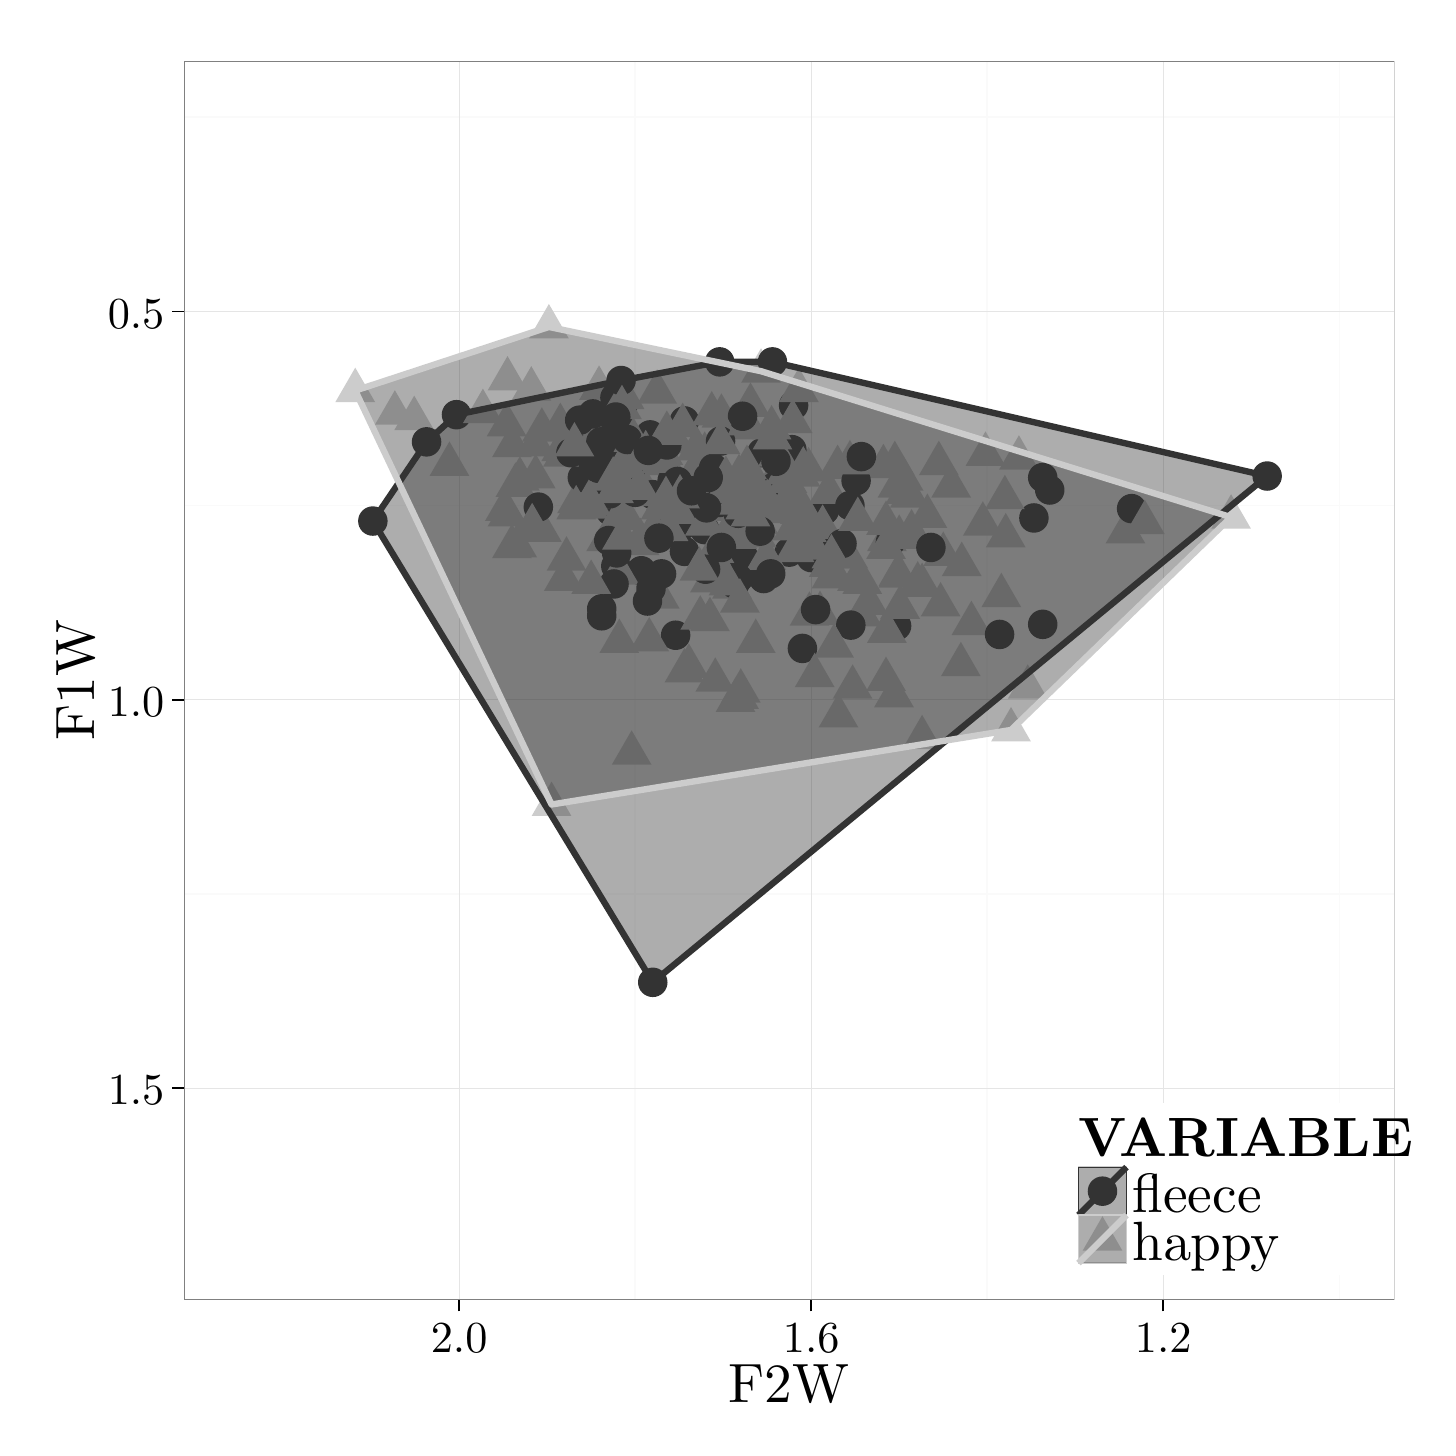
\begin{tikzpicture}[x=1pt,y=1pt]
\definecolor{fillColor}{RGB}{255,255,255}
\path[use as bounding box,fill=fillColor,fill opacity=0.00] (0,0) rectangle (505.89,505.89);
\begin{scope}
\path[clip] (  0.00,  0.00) rectangle (505.89,505.89);
\definecolor{drawColor}{RGB}{255,255,255}
\definecolor{fillColor}{RGB}{255,255,255}

\path[draw=drawColor,line width= 0.6pt,line join=round,line cap=round,fill=fillColor] (  0.00, -0.00) rectangle (505.89,505.89);
\end{scope}
\begin{scope}
\path[clip] ( 56.50, 46.31) rectangle (493.85,493.84);
\definecolor{fillColor}{RGB}{255,255,255}

\path[fill=fillColor] ( 56.50, 46.31) rectangle (493.85,493.84);
\definecolor{drawColor}{gray}{0.98}

\path[draw=drawColor,line width= 0.6pt,line join=round] ( 56.50,473.50) --
	(493.85,473.50);

\path[draw=drawColor,line width= 0.6pt,line join=round] ( 56.50,333.21) --
	(493.85,333.21);

\path[draw=drawColor,line width= 0.6pt,line join=round] ( 56.50,192.91) --
	(493.85,192.91);

\path[draw=drawColor,line width= 0.6pt,line join=round] (473.97, 46.31) --
	(473.97,493.84);

\path[draw=drawColor,line width= 0.6pt,line join=round] (346.74, 46.31) --
	(346.74,493.84);

\path[draw=drawColor,line width= 0.6pt,line join=round] (219.51, 46.31) --
	(219.51,493.84);
\definecolor{drawColor}{gray}{0.90}

\path[draw=drawColor,line width= 0.2pt,line join=round] ( 56.50,403.36) --
	(493.85,403.36);

\path[draw=drawColor,line width= 0.2pt,line join=round] ( 56.50,263.06) --
	(493.85,263.06);

\path[draw=drawColor,line width= 0.2pt,line join=round] ( 56.50,122.77) --
	(493.85,122.77);

\path[draw=drawColor,line width= 0.2pt,line join=round] (410.35, 46.31) --
	(410.35,493.84);

\path[draw=drawColor,line width= 0.2pt,line join=round] (283.13, 46.31) --
	(283.13,493.84);

\path[draw=drawColor,line width= 0.2pt,line join=round] (155.90, 46.31) --
	(155.90,493.84);
\definecolor{fillColor}{gray}{0.20}

\path[fill=fillColor] (265.95,306.83) circle (  5.33);

\path[fill=fillColor] (197.25,360.71) circle (  5.33);
\definecolor{fillColor}{gray}{0.80}

\path[fill=fillColor] (220.47,360.87) --
	(227.65,348.42) --
	(213.28,348.42) --
	cycle;
\definecolor{fillColor}{gray}{0.20}

\path[fill=fillColor] (283.13,314.41) circle (  5.33);
\definecolor{fillColor}{gray}{0.80}

\path[fill=fillColor] (254.50,312.04) --
	(261.68,299.60) --
	(247.32,299.60) --
	cycle;
\definecolor{fillColor}{gray}{0.20}

\path[fill=fillColor] (258.63,314.69) circle (  5.33);
\definecolor{fillColor}{gray}{0.80}

\path[fill=fillColor] (323.20,257.61) --
	(330.39,245.16) --
	(316.02,245.16) --
	cycle;

\path[fill=fillColor] (313.02,272.76) --
	(320.21,260.32) --
	(305.84,260.32) --
	cycle;

\path[fill=fillColor] (292.67,355.25) --
	(299.85,342.81) --
	(285.48,342.81) --
	cycle;
\definecolor{fillColor}{gray}{0.20}

\path[fill=fillColor] (289.49,319.74) circle (  5.33);

\path[fill=fillColor] (237.32,316.65) circle (  5.33);

\path[fill=fillColor] (276.76,369.40) circle (  5.33);
\definecolor{fillColor}{gray}{0.80}

\path[fill=fillColor] (264.36,345.15) --
	(271.54,332.71) --
	(257.18,332.71) --
	cycle;
\definecolor{fillColor}{gray}{0.20}

\path[fill=fillColor] (244.64,324.51) circle (  5.33);
\definecolor{fillColor}{gray}{0.80}

\path[fill=fillColor] (325.11,337.58) --
	(332.30,325.13) --
	(317.93,325.13) --
	cycle;

\path[fill=fillColor] (220.47,351.61) --
	(227.65,339.16) --
	(213.28,339.16) --
	cycle;
\definecolor{fillColor}{gray}{0.20}

\path[fill=fillColor] (257.68,307.96) circle (  5.33);
\definecolor{fillColor}{gray}{0.80}

\path[fill=fillColor] (290.44,315.69) --
	(297.63,303.25) --
	(283.26,303.25) --
	cycle;
\definecolor{fillColor}{gray}{0.20}

\path[fill=fillColor] (251.96,314.97) circle (  5.33);
\definecolor{fillColor}{gray}{0.80}

\path[fill=fillColor] (246.55,300.26) --
	(253.73,287.81) --
	(239.36,287.81) --
	cycle;

\path[fill=fillColor] (253.23,344.31) --
	(260.41,331.87) --
	(246.04,331.87) --
	cycle;

\path[fill=fillColor] (278.35,335.61) --
	(285.54,323.17) --
	(271.17,323.17) --
	cycle;

\path[fill=fillColor] (230.64,356.66) --
	(237.83,344.21) --
	(223.46,344.21) --
	cycle;

\path[fill=fillColor] (228.42,308.40) --
	(235.60,295.95) --
	(221.23,295.95) --
	cycle;

\path[fill=fillColor] (232.87,335.05) --
	(240.06,322.61) --
	(225.69,322.61) --
	cycle;
\definecolor{fillColor}{gray}{0.20}

\path[fill=fillColor] (217.60,344.71) circle (  5.33);
\definecolor{fillColor}{gray}{0.80}

\path[fill=fillColor] (242.73,351.61) --
	(249.92,339.16) --
	(235.55,339.16) --
	cycle;

\path[fill=fillColor] (301.57,301.94) --
	(308.76,289.50) --
	(294.39,289.50) --
	cycle;

\path[fill=fillColor] (221.74,360.58) --
	(228.92,348.14) --
	(214.55,348.14) --
	cycle;

\path[fill=fillColor] (207.43,370.97) --
	(214.61,358.52) --
	(200.24,358.52) --
	cycle;

\path[fill=fillColor] (192.48,370.41) --
	(199.66,357.96) --
	(185.29,357.96) --
	cycle;

\path[fill=fillColor] (215.38,338.70) --
	(222.56,326.25) --
	(208.19,326.25) --
	cycle;

\path[fill=fillColor] (206.47,383.87) --
	(213.66,371.43) --
	(199.29,371.43) --
	cycle;

\path[fill=fillColor] (272.31,339.26) --
	(279.50,326.82) --
	(265.13,326.82) --
	cycle;

\path[fill=fillColor] (248.14,324.95) --
	(255.32,312.51) --
	(240.95,312.51) --
	cycle;

\path[fill=fillColor] (212.52,369.84) --
	(219.70,357.40) --
	(205.33,357.40) --
	cycle;
\definecolor{fillColor}{gray}{0.20}

\path[fill=fillColor] (232.87,342.19) circle (  5.33);
\definecolor{fillColor}{gray}{0.80}

\path[fill=fillColor] (215.38,354.13) --
	(222.56,341.69) --
	(208.19,341.69) --
	cycle;
\definecolor{fillColor}{gray}{0.20}

\path[fill=fillColor] (237.32,363.79) circle (  5.33);
\definecolor{fillColor}{gray}{0.80}

\path[fill=fillColor] (229.05,357.50) --
	(236.24,345.05) --
	(221.87,345.05) --
	cycle;
\definecolor{fillColor}{gray}{0.20}

\path[fill=fillColor] (210.61,331.24) circle (  5.33);

\path[fill=fillColor] (215.06,369.40) circle (  5.33);
\definecolor{fillColor}{gray}{0.80}

\path[fill=fillColor] (271.99,352.73) --
	(279.18,340.28) --
	(264.81,340.28) --
	cycle;
\definecolor{fillColor}{gray}{0.20}

\path[fill=fillColor] (275.17,316.37) circle (  5.33);
\definecolor{fillColor}{gray}{0.80}

\path[fill=fillColor] (238.91,350.20) --
	(246.10,337.76) --
	(231.73,337.76) --
	cycle;
\definecolor{fillColor}{gray}{0.20}

\path[fill=fillColor] (213.47,363.23) circle (  5.33);
\definecolor{fillColor}{gray}{0.80}

\path[fill=fillColor] (249.41,347.40) --
	(256.60,334.95) --
	(242.23,334.95) --
	cycle;

\path[fill=fillColor] (321.61,313.17) --
	(328.80,300.72) --
	(314.43,300.72) --
	cycle;

\path[fill=fillColor] (333.70,348.52) --
	(340.88,336.08) --
	(326.51,336.08) --
	cycle;

\path[fill=fillColor] (282.17,354.41) --
	(289.36,341.97) --
	(274.99,341.97) --
	cycle;
\definecolor{fillColor}{gray}{0.20}

\path[fill=fillColor] (234.78,341.91) circle (  5.33);

\path[fill=fillColor] (369.32,338.82) circle (  5.33);

\path[fill=fillColor] (287.90,331.52) circle (  5.33);
\definecolor{fillColor}{gray}{0.80}

\path[fill=fillColor] (257.04,369.56) --
	(264.23,357.12) --
	(249.86,357.12) --
	cycle;

\path[fill=fillColor] (220.15,358.90) --
	(227.33,346.46) --
	(212.96,346.46) --
	cycle;
\definecolor{fillColor}{gray}{0.20}

\path[fill=fillColor] (225.87,160.93) circle (  5.33);
\definecolor{fillColor}{gray}{0.80}

\path[fill=fillColor] (263.41,330.56) --
	(270.59,318.12) --
	(256.22,318.12) --
	cycle;

\path[fill=fillColor] (275.17,354.13) --
	(282.36,341.69) --
	(267.99,341.69) --
	cycle;
\definecolor{fillColor}{gray}{0.20}

\path[fill=fillColor] (212.20,372.21) circle (  5.33);
\definecolor{fillColor}{gray}{0.80}

\path[fill=fillColor] (276.45,340.38) --
	(283.63,327.94) --
	(269.26,327.94) --
	cycle;
\definecolor{fillColor}{gray}{0.20}

\path[fill=fillColor] (265.31,352.29) circle (  5.33);
\definecolor{fillColor}{gray}{0.80}

\path[fill=fillColor] (283.76,326.07) --
	(290.95,313.63) --
	(276.58,313.63) --
	cycle;

\path[fill=fillColor] (241.78,361.99) --
	(248.96,349.54) --
	(234.59,349.54) --
	cycle;

\path[fill=fillColor] (217.60,347.96) --
	(224.79,335.51) --
	(210.42,335.51) --
	cycle;

\path[fill=fillColor] (267.86,347.68) --
	(275.04,335.23) --
	(260.67,335.23) --
	cycle;

\path[fill=fillColor] (251.64,340.10) --
	(258.82,327.66) --
	(244.45,327.66) --
	cycle;
\definecolor{fillColor}{gray}{0.20}

\path[fill=fillColor] (276.13,353.41) circle (  5.33);
\definecolor{fillColor}{gray}{0.80}

\path[fill=fillColor] (286.31,302.50) --
	(293.49,290.06) --
	(279.12,290.06) --
	cycle;

\path[fill=fillColor] (313.34,356.66) --
	(320.53,344.21) --
	(306.16,344.21) --
	cycle;

\path[fill=fillColor] (227.46,382.47) --
	(234.65,370.03) --
	(220.28,370.03) --
	cycle;

\path[fill=fillColor] (301.57,313.73) --
	(308.76,301.28) --
	(294.39,301.28) --
	cycle;

\path[fill=fillColor] (355.33,260.42) --
	(362.51,247.97) --
	(348.14,247.97) --
	cycle;

\path[fill=fillColor] (198.52,342.91) --
	(205.71,330.46) --
	(191.34,330.46) --
	cycle;

\path[fill=fillColor] (250.68,373.77) --
	(257.87,361.33) --
	(243.50,361.33) --
	cycle;

\path[fill=fillColor] (176.89,326.91) --
	(184.08,314.47) --
	(169.71,314.47) --
	cycle;

\path[fill=fillColor] (189.30,233.48) --
	(196.48,221.03) --
	(182.11,221.03) --
	cycle;

\path[fill=fillColor] (173.39,387.24) --
	(180.58,374.80) --
	(166.21,374.80) --
	cycle;

\path[fill=fillColor] (183.57,363.39) --
	(190.76,350.95) --
	(176.39,350.95) --
	cycle;

\path[fill=fillColor] (281.54,332.53) --
	(288.72,320.08) --
	(274.35,320.08) --
	cycle;

\path[fill=fillColor] (215.70,380.51) --
	(222.88,368.06) --
	(208.51,368.06) --
	cycle;

\path[fill=fillColor] (185.80,368.72) --
	(192.98,356.28) --
	(178.61,356.28) --
	cycle;
\definecolor{fillColor}{gray}{0.20}

\path[fill=fillColor] (200.43,343.31) circle (  5.33);
\definecolor{fillColor}{gray}{0.80}

\path[fill=fillColor] (205.52,366.76) --
	(212.70,354.31) --
	(198.33,354.31) --
	cycle;
\definecolor{fillColor}{gray}{0.20}

\path[fill=fillColor] (212.83,350.32) circle (  5.33);
\definecolor{fillColor}{gray}{0.80}

\path[fill=fillColor] (246.55,314.29) --
	(253.73,301.84) --
	(239.36,301.84) --
	cycle;

\path[fill=fillColor] (263.09,292.40) --
	(270.27,279.96) --
	(255.90,279.96) --
	cycle;
\definecolor{fillColor}{gray}{0.20}

\path[fill=fillColor] (212.52,311.32) circle (  5.33);

\path[fill=fillColor] (366.78,290.28) circle (  5.33);
\definecolor{fillColor}{gray}{0.80}

\path[fill=fillColor] (255.14,335.05) --
	(262.32,322.61) --
	(247.95,322.61) --
	cycle;
\definecolor{fillColor}{gray}{0.20}

\path[fill=fillColor] (236.37,325.91) circle (  5.33);

\path[fill=fillColor] (230.01,331.52) circle (  5.33);
\definecolor{fillColor}{gray}{0.80}

\path[fill=fillColor] (289.49,319.90) --
	(296.67,307.46) --
	(282.30,307.46) --
	cycle;

\path[fill=fillColor] (314.61,316.53) --
	(321.80,304.09) --
	(307.43,304.09) --
	cycle;

\path[fill=fillColor] (303.80,306.15) --
	(310.99,293.71) --
	(296.62,293.71) --
	cycle;

\path[fill=fillColor] (319.39,331.96) --
	(326.57,319.52) --
	(312.20,319.52) --
	cycle;

\path[fill=fillColor] (244.64,360.02) --
	(251.82,347.58) --
	(237.46,347.58) --
	cycle;
\definecolor{fillColor}{gray}{0.20}

\path[fill=fillColor] (269.77,339.94) circle (  5.33);

\path[fill=fillColor] (212.52,362.67) circle (  5.33);

\path[fill=fillColor] (297.44,290.00) circle (  5.33);
\definecolor{fillColor}{gray}{0.80}

\path[fill=fillColor] (279.31,352.45) --
	(286.49,340.00) --
	(272.12,340.00) --
	cycle;

\path[fill=fillColor] (232.55,342.91) --
	(239.74,330.46) --
	(225.37,330.46) --
	cycle;
\definecolor{fillColor}{gray}{0.20}

\path[fill=fillColor] (234.14,286.35) circle (  5.33);
\definecolor{fillColor}{gray}{0.80}

\path[fill=fillColor] (310.48,329.16) --
	(317.66,316.71) --
	(303.29,316.71) --
	cycle;

\path[fill=fillColor] (351.83,308.96) --
	(359.01,296.51) --
	(344.64,296.51) --
	cycle;
\definecolor{fillColor}{gray}{0.20}

\path[fill=fillColor] (246.55,341.63) circle (  5.33);
\definecolor{fillColor}{gray}{0.80}

\path[fill=fillColor] (243.05,300.82) --
	(250.23,288.38) --
	(235.86,288.38) --
	cycle;
\definecolor{fillColor}{gray}{0.20}

\path[fill=fillColor] (223.97,298.70) circle (  5.33);
\definecolor{fillColor}{gray}{0.80}

\path[fill=fillColor] (337.20,283.98) --
	(344.38,271.54) --
	(330.01,271.54) --
	cycle;

\path[fill=fillColor] (262.13,344.59) --
	(269.32,332.15) --
	(254.95,332.15) --
	cycle;

\path[fill=fillColor] (277.08,325.23) --
	(284.27,312.79) --
	(269.90,312.79) --
	cycle;

\path[fill=fillColor] (261.18,333.37) --
	(268.36,320.92) --
	(253.99,320.92) --
	cycle;

\path[fill=fillColor] (316.52,351.04) --
	(323.71,338.60) --
	(309.34,338.60) --
	cycle;
\definecolor{fillColor}{gray}{0.20}

\path[fill=fillColor] (247.82,346.68) circle (  5.33);
\definecolor{fillColor}{gray}{0.80}

\path[fill=fillColor] (282.49,302.22) --
	(289.67,289.78) --
	(275.30,289.78) --
	cycle;

\path[fill=fillColor] (281.54,333.93) --
	(288.72,321.48) --
	(274.35,321.48) --
	cycle;

\path[fill=fillColor] (291.40,290.72) --
	(298.58,278.27) --
	(284.21,278.27) --
	cycle;

\path[fill=fillColor] (337.52,320.18) --
	(344.70,307.74) --
	(330.33,307.74) --
	cycle;

\path[fill=fillColor] (271.04,359.74) --
	(278.22,347.30) --
	(263.85,347.30) --
	cycle;

\path[fill=fillColor] (216.33,358.34) --
	(223.52,345.90) --
	(209.15,345.90) --
	cycle;

\path[fill=fillColor] (274.54,350.20) --
	(281.72,337.76) --
	(267.35,337.76) --
	cycle;

\path[fill=fillColor] (221.10,327.76) --
	(228.29,315.31) --
	(213.92,315.31) --
	cycle;

\path[fill=fillColor] (259.91,355.25) --
	(267.09,342.81) --
	(252.72,342.81) --
	cycle;

\path[fill=fillColor] (215.38,348.24) --
	(222.56,335.79) --
	(208.19,335.79) --
	cycle;

\path[fill=fillColor] (251.00,317.09) --
	(258.19,304.65) --
	(243.82,304.65) --
	cycle;

\path[fill=fillColor] (228.74,340.66) --
	(235.92,328.22) --
	(221.55,328.22) --
	cycle;

\path[fill=fillColor] (213.47,336.73) --
	(220.65,324.29) --
	(206.28,324.29) --
	cycle;
\definecolor{fillColor}{gray}{0.20}

\path[fill=fillColor] (207.43,293.37) circle (  5.33);
\definecolor{fillColor}{gray}{0.80}

\path[fill=fillColor] (250.05,346.84) --
	(257.23,334.39) --
	(242.86,334.39) --
	cycle;
\definecolor{fillColor}{gray}{0.20}

\path[fill=fillColor] (225.87,337.14) circle (  5.33);
\definecolor{fillColor}{gray}{0.80}

\path[fill=fillColor] (341.01,298.86) --
	(348.20,286.41) --
	(333.83,286.41) --
	cycle;
\definecolor{fillColor}{gray}{0.20}

\path[fill=fillColor] (279.95,281.58) circle (  5.33);

\path[fill=fillColor] (255.45,304.87) circle (  5.33);
\definecolor{fillColor}{gray}{0.80}

\path[fill=fillColor] (257.04,351.89) --
	(264.23,339.44) --
	(249.86,339.44) --
	cycle;
\definecolor{fillColor}{gray}{0.20}

\path[fill=fillColor] (284.72,295.61) circle (  5.33);
\definecolor{fillColor}{gray}{0.80}

\path[fill=fillColor] (266.90,322.42) --
	(274.09,309.98) --
	(259.72,309.98) --
	cycle;
\definecolor{fillColor}{gray}{0.20}

\path[fill=fillColor] (232.87,340.22) circle (  5.33);
\definecolor{fillColor}{gray}{0.80}

\path[fill=fillColor] (263.72,333.37) --
	(270.91,320.92) --
	(256.54,320.92) --
	cycle;

\path[fill=fillColor] (227.15,362.83) --
	(234.33,350.38) --
	(219.96,350.38) --
	cycle;

\path[fill=fillColor] (252.27,351.33) --
	(259.46,338.88) --
	(245.09,338.88) --
	cycle;
\definecolor{fillColor}{gray}{0.20}

\path[fill=fillColor] (250.05,334.33) circle (  5.33);

\path[fill=fillColor] (250.37,356.50) circle (  5.33);

\path[fill=fillColor] (261.18,325.63) circle (  5.33);
\definecolor{fillColor}{gray}{0.80}

\path[fill=fillColor] (314.30,348.52) --
	(321.48,336.08) --
	(307.11,336.08) --
	cycle;
\definecolor{fillColor}{gray}{0.20}

\path[fill=fillColor] (214.42,378.38) circle (  5.33);
\definecolor{fillColor}{gray}{0.80}

\path[fill=fillColor] (273.90,353.29) --
	(281.09,340.84) --
	(266.72,340.84) --
	cycle;
\definecolor{fillColor}{gray}{0.20}

\path[fill=fillColor] (256.73,306.83) circle (  5.33);

\path[fill=fillColor] (313.98,289.72) circle (  5.33);
\definecolor{fillColor}{gray}{0.80}

\path[fill=fillColor] (214.74,376.86) --
	(221.93,364.41) --
	(207.56,364.41) --
	cycle;

\path[fill=fillColor] (329.88,305.59) --
	(337.07,293.15) --
	(322.70,293.15) --
	cycle;

\path[fill=fillColor] (310.16,278.65) --
	(317.35,266.21) --
	(302.98,266.21) --
	cycle;

\path[fill=fillColor] (209.02,329.16) --
	(216.20,316.71) --
	(201.83,316.71) --
	cycle;
\definecolor{fillColor}{gray}{0.20}

\path[fill=fillColor] (224.92,358.74) circle (  5.33);
\definecolor{fillColor}{gray}{0.80}

\path[fill=fillColor] (292.99,265.47) --
	(300.17,253.02) --
	(285.80,253.02) --
	cycle;

\path[fill=fillColor] (345.15,334.77) --
	(352.33,322.33) --
	(337.96,322.33) --
	cycle;

\path[fill=fillColor] (259.91,370.97) --
	(267.09,358.52) --
	(252.72,358.52) --
	cycle;

\path[fill=fillColor] (219.83,345.43) --
	(227.02,332.99) --
	(212.65,332.99) --
	cycle;

\path[fill=fillColor] (204.56,345.71) --
	(211.75,333.27) --
	(197.38,333.27) --
	cycle;

\path[fill=fillColor] (213.79,292.40) --
	(220.97,279.96) --
	(206.60,279.96) --
	cycle;

\path[fill=fillColor] (223.33,360.58) --
	(230.51,348.14) --
	(216.14,348.14) --
	cycle;

\path[fill=fillColor] (211.56,350.20) --
	(218.75,337.76) --
	(204.38,337.76) --
	cycle;

\path[fill=fillColor] (236.69,370.41) --
	(243.87,357.96) --
	(229.50,357.96) --
	cycle;
\definecolor{fillColor}{gray}{0.20}

\path[fill=fillColor] (221.74,309.64) circle (  5.33);
\definecolor{fillColor}{gray}{0.80}

\path[fill=fillColor] (193.43,359.74) --
	(200.62,347.30) --
	(186.25,347.30) --
	cycle;

\path[fill=fillColor] (218.24,252.00) --
	(225.43,239.55) --
	(211.06,239.55) --
	cycle;

\path[fill=fillColor] (310.48,296.05) --
	(317.66,283.61) --
	(303.29,283.61) --
	cycle;
\definecolor{fillColor}{gray}{0.20}

\path[fill=fillColor] (244.96,310.20) circle (  5.33);
\definecolor{fillColor}{gray}{0.80}

\path[fill=fillColor] (152.40,356.38) --
	(159.59,343.93) --
	(145.22,343.93) --
	cycle;
\definecolor{fillColor}{gray}{0.20}

\path[fill=fillColor] (311.75,320.02) circle (  5.33);

\path[fill=fillColor] (154.95,366.04) circle (  5.33);
\definecolor{fillColor}{gray}{0.80}

\path[fill=fillColor] (132.68,374.89) --
	(139.87,362.45) --
	(125.50,362.45) --
	cycle;

\path[fill=fillColor] (213.79,317.09) --
	(220.97,304.65) --
	(206.60,304.65) --
	cycle;

\path[fill=fillColor] (221.42,328.88) --
	(228.61,316.43) --
	(214.24,316.43) --
	cycle;

\path[fill=fillColor] (278.67,383.03) --
	(285.86,370.59) --
	(271.49,370.59) --
	cycle;
\definecolor{fillColor}{gray}{0.20}

\path[fill=fillColor] (250.05,385.12) circle (  5.33);

\path[fill=fillColor] (204.25,366.32) circle (  5.33);
\definecolor{fillColor}{gray}{0.80}

\path[fill=fillColor] (188.34,406.04) --
	(195.53,393.60) --
	(181.16,393.60) --
	cycle;

\path[fill=fillColor] (265.00,390.05) --
	(272.18,377.60) --
	(257.81,377.60) --
	cycle;
\definecolor{fillColor}{gray}{0.20}

\path[fill=fillColor] (269.13,385.12) circle (  5.33);
\definecolor{fillColor}{gray}{0.80}

\path[fill=fillColor] (251.64,346.56) --
	(258.82,334.11) --
	(244.45,334.11) --
	cycle;

\path[fill=fillColor] (234.14,364.51) --
	(241.33,352.07) --
	(226.96,352.07) --
	cycle;
\definecolor{fillColor}{gray}{0.20}

\path[fill=fillColor] (447.88,343.87) circle (  5.33);
\definecolor{fillColor}{gray}{0.80}

\path[fill=fillColor] (261.18,377.70) --
	(268.36,365.26) --
	(253.99,365.26) --
	cycle;
\definecolor{fillColor}{gray}{0.20}

\path[fill=fillColor] (124.73,327.60) circle (  5.33);
\definecolor{fillColor}{gray}{0.80}

\path[fill=fillColor] (236.69,342.07) --
	(243.87,329.62) --
	(229.50,329.62) --
	cycle;

\path[fill=fillColor] (192.80,361.71) --
	(199.98,349.26) --
	(185.61,349.26) --
	cycle;

\path[fill=fillColor] (229.69,360.30) --
	(236.88,347.86) --
	(222.51,347.86) --
	cycle;

\path[fill=fillColor] (164.49,375.46) --
	(171.67,363.01) --
	(157.30,363.01) --
	cycle;

\path[fill=fillColor] (215.38,337.58) --
	(222.56,325.13) --
	(208.19,325.13) --
	cycle;

\path[fill=fillColor] (358.19,358.62) --
	(365.37,346.18) --
	(351.00,346.18) --
	cycle;
\definecolor{fillColor}{gray}{0.20}

\path[fill=fillColor] (212.52,365.20) circle (  5.33);
\definecolor{fillColor}{gray}{0.80}

\path[fill=fillColor] (434.84,337.30) --
	(442.03,324.85) --
	(427.66,324.85) --
	cycle;

\path[fill=fillColor] (278.67,341.22) --
	(285.86,328.78) --
	(271.49,328.78) --
	cycle;

\path[fill=fillColor] (250.37,364.23) --
	(257.55,351.79) --
	(243.18,351.79) --
	cycle;

\path[fill=fillColor] (256.41,330.00) --
	(263.59,317.56) --
	(249.22,317.56) --
	cycle;

\path[fill=fillColor] (174.98,363.11) --
	(182.17,350.67) --
	(167.80,350.67) --
	cycle;

\path[fill=fillColor] (139.68,372.93) --
	(146.86,360.49) --
	(132.49,360.49) --
	cycle;

\path[fill=fillColor] (218.88,365.07) --
	(226.06,352.63) --
	(211.69,352.63) --
	cycle;

\path[fill=fillColor] (118.37,383.03) --
	(125.55,370.59) --
	(111.18,370.59) --
	cycle;

\path[fill=fillColor] (181.98,383.59) --
	(189.17,371.15) --
	(174.80,371.15) --
	cycle;

\path[fill=fillColor] (173.07,370.69) --
	(180.26,358.24) --
	(165.89,358.24) --
	cycle;
\definecolor{fillColor}{gray}{0.20}

\path[fill=fillColor] (144.13,356.22) circle (  5.33);
\definecolor{fillColor}{gray}{0.80}

\path[fill=fillColor] (299.67,314.85) --
	(306.85,302.40) --
	(292.48,302.40) --
	cycle;
\definecolor{fillColor}{gray}{0.20}

\path[fill=fillColor] (211.88,304.87) circle (  5.33);

\path[fill=fillColor] (204.25,348.92) circle (  5.33);
\definecolor{fillColor}{gray}{0.80}

\path[fill=fillColor] (280.26,354.69) --
	(287.45,342.25) --
	(273.08,342.25) --
	cycle;
\definecolor{fillColor}{gray}{0.20}

\path[fill=fillColor] (199.47,364.07) circle (  5.33);
\definecolor{fillColor}{gray}{0.80}

\path[fill=fillColor] (252.91,331.68) --
	(260.09,319.24) --
	(245.72,319.24) --
	cycle;
\definecolor{fillColor}{gray}{0.20}

\path[fill=fillColor] (196.29,352.29) circle (  5.33);
\definecolor{fillColor}{gray}{0.80}

\path[fill=fillColor] (264.04,335.33) --
	(271.23,322.89) --
	(256.86,322.89) --
	cycle;

\path[fill=fillColor] (255.77,271.08) --
	(262.96,258.63) --
	(248.59,258.63) --
	cycle;

\path[fill=fillColor] (309.21,355.53) --
	(316.39,343.09) --
	(302.02,343.09) --
	cycle;

\path[fill=fillColor] (268.81,369.56) --
	(276.00,357.12) --
	(261.63,357.12) --
	cycle;
\definecolor{fillColor}{gray}{0.20}

\path[fill=fillColor] (216.65,357.06) circle (  5.33);

\path[fill=fillColor] (258.32,365.48) circle (  5.33);

\path[fill=fillColor] (299.35,342.19) circle (  5.33);
\definecolor{fillColor}{gray}{0.80}

\path[fill=fillColor] (276.45,371.81) --
	(283.63,359.36) --
	(269.26,359.36) --
	cycle;

\path[fill=fillColor] (274.22,342.91) --
	(281.40,330.46) --
	(267.04,330.46) --
	cycle;
\definecolor{fillColor}{gray}{0.20}

\path[fill=fillColor] (207.11,356.22) circle (  5.33);
\definecolor{fillColor}{gray}{0.80}

\path[fill=fillColor] (318.75,344.87) --
	(325.93,332.43) --
	(311.56,332.43) --
	cycle;

\path[fill=fillColor] (314.93,330.00) --
	(322.12,317.56) --
	(307.75,317.56) --
	cycle;
\definecolor{fillColor}{gray}{0.20}

\path[fill=fillColor] (230.96,355.09) circle (  5.33);
\definecolor{fillColor}{gray}{0.80}

\path[fill=fillColor] (263.41,347.96) --
	(270.59,335.51) --
	(256.22,335.51) --
	cycle;
\definecolor{fillColor}{gray}{0.20}

\path[fill=fillColor] (366.78,343.31) circle (  5.33);
\definecolor{fillColor}{gray}{0.80}

\path[fill=fillColor] (296.48,322.99) --
	(303.67,310.54) --
	(289.30,310.54) --
	cycle;

\path[fill=fillColor] (239.23,339.26) --
	(246.42,326.82) --
	(232.05,326.82) --
	cycle;

\path[fill=fillColor] (317.16,346.27) --
	(324.34,333.83) --
	(309.97,333.83) --
	cycle;

\path[fill=fillColor] (230.96,367.60) --
	(238.15,355.15) --
	(223.78,355.15) --
	cycle;

\path[fill=fillColor] (257.68,274.44) --
	(264.87,262.00) --
	(250.50,262.00) --
	cycle;

\path[fill=fillColor] (209.65,344.59) --
	(216.84,332.15) --
	(202.47,332.15) --
	cycle;
\definecolor{fillColor}{gray}{0.20}

\path[fill=fillColor] (206.15,346.68) circle (  5.33);
\definecolor{fillColor}{gray}{0.80}

\path[fill=fillColor] (298.08,275.85) --
	(305.26,263.40) --
	(290.89,263.40) --
	cycle;

\path[fill=fillColor] (346.10,360.02) --
	(353.29,347.58) --
	(338.92,347.58) --
	cycle;

\path[fill=fillColor] (276.45,333.09) --
	(283.63,320.64) --
	(269.26,320.64) --
	cycle;

\path[fill=fillColor] (353.42,330.56) --
	(360.60,318.12) --
	(346.23,318.12) --
	cycle;

\path[fill=fillColor] (230.64,344.03) --
	(237.83,331.59) --
	(223.46,331.59) --
	cycle;

\path[fill=fillColor] (202.66,340.94) --
	(209.84,328.50) --
	(195.47,328.50) --
	cycle;

\path[fill=fillColor] (289.49,346.27) --
	(296.67,333.83) --
	(282.30,333.83) --
	cycle;

\path[fill=fillColor] (173.39,338.14) --
	(180.58,325.69) --
	(166.21,325.69) --
	cycle;

\path[fill=fillColor] (329.25,356.66) --
	(336.43,344.21) --
	(322.06,344.21) --
	cycle;

\path[fill=fillColor] (257.04,344.87) --
	(264.23,332.43) --
	(249.86,332.43) --
	cycle;

\path[fill=fillColor] (198.20,340.66) --
	(205.39,328.22) --
	(191.02,328.22) --
	cycle;

\path[fill=fillColor] (222.06,358.90) --
	(229.24,346.46) --
	(214.87,346.46) --
	cycle;

\path[fill=fillColor] (172.44,340.10) --
	(179.62,327.66) --
	(165.25,327.66) --
	cycle;
\definecolor{fillColor}{gray}{0.20}

\path[fill=fillColor] (297.12,333.21) circle (  5.33);
\definecolor{fillColor}{gray}{0.80}

\path[fill=fillColor] (197.57,363.39) --
	(204.75,350.95) --
	(190.38,350.95) --
	cycle;
\definecolor{fillColor}{gray}{0.20}

\path[fill=fillColor] (210.29,337.42) circle (  5.33);
\definecolor{fillColor}{gray}{0.80}

\path[fill=fillColor] (237.32,281.74) --
	(244.51,269.30) --
	(230.14,269.30) --
	cycle;
\definecolor{fillColor}{gray}{0.20}

\path[fill=fillColor] (219.51,337.98) circle (  5.33);

\path[fill=fillColor] (212.83,316.09) circle (  5.33);
\definecolor{fillColor}{gray}{0.80}

\path[fill=fillColor] (278.99,338.98) --
	(286.18,326.54) --
	(271.81,326.54) --
	cycle;
\definecolor{fillColor}{gray}{0.20}

\path[fill=fillColor] (244.00,330.96) circle (  5.33);
\definecolor{fillColor}{gray}{0.80}

\path[fill=fillColor] (396.68,331.96) --
	(403.86,319.52) --
	(389.49,319.52) --
	cycle;
\definecolor{fillColor}{gray}{0.20}

\path[fill=fillColor] (270.40,349.20) circle (  5.33);
\definecolor{fillColor}{gray}{0.80}

\path[fill=fillColor] (253.23,313.17) --
	(260.41,300.72) --
	(246.04,300.72) --
	cycle;

\path[fill=fillColor] (242.73,318.50) --
	(249.92,306.05) --
	(235.55,306.05) --
	cycle;

\path[fill=fillColor] (226.19,332.53) --
	(233.38,320.08) --
	(219.01,320.08) --
	cycle;

\path[fill=fillColor] (267.22,342.91) --
	(274.41,330.46) --
	(260.04,330.46) --
	cycle;
\definecolor{fillColor}{gray}{0.20}

\path[fill=fillColor] (256.73,330.40) circle (  5.33);

\path[fill=fillColor] (224.28,353.13) circle (  5.33);

\path[fill=fillColor] (225.24,303.19) circle (  5.33);
\definecolor{fillColor}{gray}{0.80}

\path[fill=fillColor] (268.18,341.50) --
	(275.36,329.06) --
	(260.99,329.06) --
	cycle;

\path[fill=fillColor] (287.26,333.65) --
	(294.45,321.20) --
	(280.08,321.20) --
	cycle;
\definecolor{fillColor}{gray}{0.20}

\path[fill=fillColor] (245.91,343.31) circle (  5.33);
\definecolor{fillColor}{gray}{0.80}

\path[fill=fillColor] (244.64,334.77) --
	(251.82,322.33) --
	(237.46,322.33) --
	cycle;

\path[fill=fillColor] (259.27,340.66) --
	(266.46,328.22) --
	(252.09,328.22) --
	cycle;
\definecolor{fillColor}{gray}{0.20}

\path[fill=fillColor] (363.60,328.72) circle (  5.33);
\definecolor{fillColor}{gray}{0.80}

\path[fill=fillColor] (174.98,326.63) --
	(182.17,314.19) --
	(167.80,314.19) --
	cycle;
\definecolor{fillColor}{gray}{0.20}

\path[fill=fillColor] (294.26,319.46) circle (  5.33);
\definecolor{fillColor}{gray}{0.80}

\path[fill=fillColor] (238.91,283.42) --
	(246.10,270.98) --
	(231.73,270.98) --
	cycle;

\path[fill=fillColor] (256.09,342.35) --
	(263.28,329.90) --
	(248.91,329.90) --
	cycle;

\path[fill=fillColor] (185.80,332.53) --
	(192.98,320.08) --
	(178.61,320.08) --
	cycle;

\path[fill=fillColor] (194.70,322.14) --
	(201.89,309.70) --
	(187.52,309.70) --
	cycle;

\path[fill=fillColor] (214.74,348.80) --
	(221.93,336.36) --
	(207.56,336.36) --
	cycle;
\definecolor{fillColor}{gray}{0.20}

\path[fill=fillColor] (245.28,332.37) circle (  5.33);
\definecolor{fillColor}{gray}{0.80}

\path[fill=fillColor] (224.60,292.96) --
	(231.79,280.52) --
	(217.42,280.52) --
	cycle;

\path[fill=fillColor] (299.98,336.45) --
	(307.17,324.01) --
	(292.80,324.01) --
	cycle;

\path[fill=fillColor] (247.18,374.61) --
	(254.37,362.17) --
	(240.00,362.17) --
	cycle;

\path[fill=fillColor] (261.50,345.99) --
	(268.68,333.55) --
	(254.31,333.55) --
	cycle;

\path[fill=fillColor] (269.13,365.92) --
	(276.32,353.47) --
	(261.95,353.47) --
	cycle;

\path[fill=fillColor] (231.60,332.81) --
	(238.78,320.36) --
	(224.41,320.36) --
	cycle;

\path[fill=fillColor] (203.61,342.07) --
	(210.79,329.62) --
	(196.42,329.62) --
	cycle;

\path[fill=fillColor] (193.75,314.85) --
	(200.93,302.40) --
	(186.56,302.40) --
	cycle;

\path[fill=fillColor] (248.46,278.37) --
	(255.64,265.93) --
	(241.27,265.93) --
	cycle;

\path[fill=fillColor] (177.85,351.04) --
	(185.03,338.60) --
	(170.66,338.60) --
	cycle;

\path[fill=fillColor] (235.73,344.59) --
	(242.92,332.15) --
	(228.55,332.15) --
	cycle;

\path[fill=fillColor] (235.10,338.98) --
	(242.28,326.54) --
	(227.91,326.54) --
	cycle;

\path[fill=fillColor] (211.56,351.04) --
	(218.75,338.60) --
	(204.38,338.60) --
	cycle;

\path[fill=fillColor] (211.88,346.56) --
	(219.06,334.11) --
	(204.69,334.11) --
	cycle;
\definecolor{fillColor}{gray}{0.20}

\path[fill=fillColor] (228.10,321.42) circle (  5.33);
\definecolor{fillColor}{gray}{0.80}

\path[fill=fillColor] (176.26,348.80) --
	(183.44,336.36) --
	(169.07,336.36) --
	cycle;
\definecolor{fillColor}{gray}{0.20}

\path[fill=fillColor] (239.87,338.54) circle (  5.33);
\definecolor{fillColor}{gray}{0.80}

\path[fill=fillColor] (323.20,312.60) --
	(330.39,300.16) --
	(316.02,300.16) --
	cycle;
\definecolor{fillColor}{gray}{0.20}

\path[fill=fillColor] (268.49,308.52) circle (  5.33);

\path[fill=fillColor] (209.97,320.58) circle (  5.33);
\definecolor{fillColor}{gray}{0.80}

\path[fill=fillColor] (310.16,326.35) --
	(317.35,313.91) --
	(302.98,313.91) --
	cycle;
\definecolor{fillColor}{gray}{0.20}

\path[fill=fillColor] (264.68,323.95) circle (  5.33);

\path[fill=fillColor] (398.90,332.09) circle (  5.33);
\definecolor{fillColor}{gray}{0.80}

\path[fill=fillColor] (315.25,304.75) --
	(322.44,292.30) --
	(308.07,292.30) --
	cycle;

\path[fill=fillColor] (257.04,272.20) --
	(264.23,259.76) --
	(249.86,259.76) --
	cycle;

\path[fill=fillColor] (261.18,338.14) --
	(268.36,325.69) --
	(253.99,325.69) --
	cycle;

\path[fill=fillColor] (310.16,335.05) --
	(317.35,322.61) --
	(302.98,322.61) --
	cycle;
\definecolor{fillColor}{gray}{0.20}

\path[fill=fillColor] (229.05,308.52) circle (  5.33);

\path[fill=fillColor] (184.53,332.65) circle (  5.33);

\path[fill=fillColor] (207.43,295.89) circle (  5.33);
\definecolor{fillColor}{gray}{0.80}

\path[fill=fillColor] (403.67,335.33) --
	(410.86,322.89) --
	(396.49,322.89) --
	cycle;
\definecolor{fillColor}{gray}{0.20}

\path[fill=fillColor] (250.68,318.06) circle (  5.33);
\definecolor{fillColor}{gray}{0.80}

\path[fill=fillColor] (314.61,315.97) --
	(321.80,303.53) --
	(307.43,303.53) --
	cycle;

\path[fill=fillColor] (257.36,306.99) --
	(264.55,294.55) --
	(250.18,294.55) --
	cycle;

\path[fill=fillColor] (290.44,322.99) --
	(297.63,310.54) --
	(283.26,310.54) --
	cycle;
\definecolor{fillColor}{gray}{0.20}

\path[fill=fillColor] (351.19,286.63) circle (  5.33);
\definecolor{fillColor}{gray}{0.80}

\path[fill=fillColor] (284.40,280.06) --
	(291.58,267.61) --
	(277.21,267.61) --
	cycle;

\path[fill=fillColor] (297.12,356.94) --
	(304.31,344.49) --
	(289.94,344.49) --
	cycle;

\path[fill=fillColor] (330.84,323.83) --
	(338.02,311.38) --
	(323.65,311.38) --
	cycle;

\path[fill=fillColor] (221.10,347.68) --
	(228.29,335.23) --
	(213.92,335.23) --
	cycle;
\definecolor{fillColor}{gray}{0.20}

\path[fill=fillColor] (301.26,350.89) circle (  5.33);
\definecolor{fillColor}{gray}{0.80}

\path[fill=fillColor] (361.37,275.85) --
	(368.56,263.40) --
	(354.19,263.40) --
	cycle;

\path[fill=fillColor] (353.10,344.31) --
	(360.29,331.87) --
	(345.92,331.87) --
	cycle;

\path[fill=fillColor] (278.67,342.35) --
	(285.86,329.90) --
	(271.49,329.90) --
	cycle;

\path[fill=fillColor] (183.57,351.89) --
	(190.76,339.44) --
	(176.39,339.44) --
	cycle;

\path[fill=fillColor] (214.74,329.72) --
	(221.93,317.28) --
	(207.56,317.28) --
	cycle;

\path[fill=fillColor] (182.30,334.21) --
	(189.48,321.77) --
	(175.11,321.77) --
	cycle;

\path[fill=fillColor] (203.61,313.73) --
	(210.79,301.28) --
	(196.42,301.28) --
	cycle;
\definecolor{fillColor}{gray}{0.20}

\path[fill=fillColor] (326.38,318.06) circle (  5.33);
\definecolor{drawColor}{gray}{0.20}
\definecolor{fillColor}{RGB}{51,51,51}

\path[draw=drawColor,line width= 2.3pt,line join=round,line cap=round,fill=fillColor,fill opacity=0.40] (144.13,356.22) --
	(154.95,366.04) --
	(214.42,378.38) --
	(250.05,385.12) --
	(269.13,385.12) --
	(447.88,343.87) --
	(225.87,160.93) --
	(124.73,327.60) --
	cycle;
\definecolor{drawColor}{gray}{0.80}

\path[draw=drawColor,line width= 2.3pt,line join=round,line cap=round,fill=fillColor,fill opacity=0.40] (118.37,374.74) --
	(188.34,397.74) --
	(265.00,381.75) --
	(434.84,329.00) --
	(355.33,252.12) --
	(189.30,225.18) --
	cycle;
\definecolor{drawColor}{gray}{0.50}

\path[draw=drawColor,line width= 0.6pt,line join=round,line cap=round] ( 56.50, 46.31) rectangle (493.85,493.84);
\end{scope}
\begin{scope}
\path[clip] (  0.00,  0.00) rectangle (505.89,505.89);
\definecolor{drawColor}{RGB}{0,0,0}

\node[text=drawColor,anchor=base east,inner sep=0pt, outer sep=0pt, scale=  1.60] at ( 49.39,397.32) {0.5};

\node[text=drawColor,anchor=base east,inner sep=0pt, outer sep=0pt, scale=  1.60] at ( 49.39,257.03) {1.0};

\node[text=drawColor,anchor=base east,inner sep=0pt, outer sep=0pt, scale=  1.60] at ( 49.39,116.73) {1.5};
\end{scope}
\begin{scope}
\path[clip] (  0.00,  0.00) rectangle (505.89,505.89);
\definecolor{drawColor}{RGB}{0,0,0}

\path[draw=drawColor,line width= 0.6pt,line join=round] ( 52.24,403.36) --
	( 56.50,403.36);

\path[draw=drawColor,line width= 0.6pt,line join=round] ( 52.24,263.06) --
	( 56.50,263.06);

\path[draw=drawColor,line width= 0.6pt,line join=round] ( 52.24,122.77) --
	( 56.50,122.77);
\end{scope}
\begin{scope}
\path[clip] (  0.00,  0.00) rectangle (505.89,505.89);
\definecolor{drawColor}{RGB}{0,0,0}

\path[draw=drawColor,line width= 0.6pt,line join=round] (410.35, 42.04) --
	(410.35, 46.31);

\path[draw=drawColor,line width= 0.6pt,line join=round] (283.13, 42.04) --
	(283.13, 46.31);

\path[draw=drawColor,line width= 0.6pt,line join=round] (155.90, 42.04) --
	(155.90, 46.31);
\end{scope}
\begin{scope}
\path[clip] (  0.00,  0.00) rectangle (505.89,505.89);
\definecolor{drawColor}{RGB}{0,0,0}

\node[text=drawColor,anchor=base,inner sep=0pt, outer sep=0pt, scale=  1.60] at (410.35, 27.13) {1.2};

\node[text=drawColor,anchor=base,inner sep=0pt, outer sep=0pt, scale=  1.60] at (283.13, 27.13) {1.6};

\node[text=drawColor,anchor=base,inner sep=0pt, outer sep=0pt, scale=  1.60] at (155.90, 27.13) {2.0};
\end{scope}
\begin{scope}
\path[clip] (  0.00,  0.00) rectangle (505.89,505.89);
\definecolor{drawColor}{RGB}{0,0,0}

\node[text=drawColor,anchor=base,inner sep=0pt, outer sep=0pt, scale=  2.00] at (275.17,  9.03) {F2W};
\end{scope}
\begin{scope}
\path[clip] (  0.00,  0.00) rectangle (505.89,505.89);
\definecolor{drawColor}{RGB}{0,0,0}

\node[text=drawColor,rotate= 90.00,anchor=base,inner sep=0pt, outer sep=0pt, scale=  2.00] at ( 24.12,270.08) {F1W};
\end{scope}
\begin{scope}
\path[clip] (  0.00,  0.00) rectangle (505.89,505.89);
\definecolor{fillColor}{RGB}{255,255,255}

\path[fill=fillColor] (375.44, 55.18) rectangle (484.98,117.15);
\end{scope}
\begin{scope}
\path[clip] (  0.00,  0.00) rectangle (505.89,505.89);
\definecolor{drawColor}{RGB}{0,0,0}

\node[text=drawColor,anchor=base west,inner sep=0pt, outer sep=0pt, scale=  2.00] at (379.71, 98.13) {\bfseries VARIABLE};
\end{scope}
\begin{scope}
\path[clip] (  0.00,  0.00) rectangle (505.89,505.89);
\definecolor{drawColor}{gray}{0.80}
\definecolor{fillColor}{RGB}{255,255,255}

\path[draw=drawColor,line width= 0.6pt,line join=round,line cap=round,fill=fillColor] (379.71, 76.79) rectangle (397.06, 94.13);
\end{scope}
\begin{scope}
\path[clip] (  0.00,  0.00) rectangle (505.89,505.89);
\definecolor{fillColor}{gray}{0.20}

\path[fill=fillColor] (388.38, 85.46) circle (  5.33);
\end{scope}
\begin{scope}
\path[clip] (  0.00,  0.00) rectangle (505.89,505.89);
\definecolor{drawColor}{gray}{0.20}
\definecolor{fillColor}{RGB}{51,51,51}

\path[draw=drawColor,line width= 0.4pt,line join=round,line cap=round,fill=fillColor,fill opacity=0.40] (379.71, 76.79) rectangle (397.06, 94.13);

\path[draw=drawColor,line width= 2.3pt,line join=round] (379.71, 76.79) --
	(397.06, 94.13);
\end{scope}
\begin{scope}
\path[clip] (  0.00,  0.00) rectangle (505.89,505.89);
\definecolor{drawColor}{gray}{0.80}
\definecolor{fillColor}{RGB}{255,255,255}

\path[draw=drawColor,line width= 0.6pt,line join=round,line cap=round,fill=fillColor] (379.71, 59.44) rectangle (397.06, 76.79);
\end{scope}
\begin{scope}
\path[clip] (  0.00,  0.00) rectangle (505.89,505.89);
\definecolor{fillColor}{gray}{0.80}

\path[fill=fillColor] (388.38, 76.41) --
	(395.57, 63.97) --
	(381.20, 63.97) --
	cycle;
\end{scope}
\begin{scope}
\path[clip] (  0.00,  0.00) rectangle (505.89,505.89);
\definecolor{drawColor}{gray}{0.80}
\definecolor{fillColor}{RGB}{51,51,51}

\path[draw=drawColor,line width= 0.4pt,line join=round,line cap=round,fill=fillColor,fill opacity=0.40] (379.71, 59.44) rectangle (397.06, 76.79);

\path[draw=drawColor,line width= 2.3pt,line join=round] (379.71, 59.44) --
	(397.06, 76.79);
\end{scope}
\begin{scope}
\path[clip] (  0.00,  0.00) rectangle (505.89,505.89);
\definecolor{drawColor}{RGB}{0,0,0}

\node[text=drawColor,anchor=base west,inner sep=0pt, outer sep=0pt, scale=  2.00] at (399.22, 77.92) {fleece};
\end{scope}
\begin{scope}
\path[clip] (  0.00,  0.00) rectangle (505.89,505.89);
\definecolor{drawColor}{RGB}{0,0,0}

\node[text=drawColor,anchor=base west,inner sep=0pt, outer sep=0pt, scale=  2.00] at (399.22, 60.57) {happy};
\end{scope}
\end{tikzpicture}
} 
		\caption{middle-aged speakers}
		\label{fig.happy.space.mid}
	\end{subfigure}
	\begin{subfigure}{.49\textwidth}
		\centering
			\definecolor{shadecolor}{rgb}{0.969, 0.969, 0.969}
			\resizebox{\linewidth}{!}{% Created by tikzDevice version 0.8.1 on 2016-02-09 02:14:19
% !TEX encoding = UTF-8 Unicode
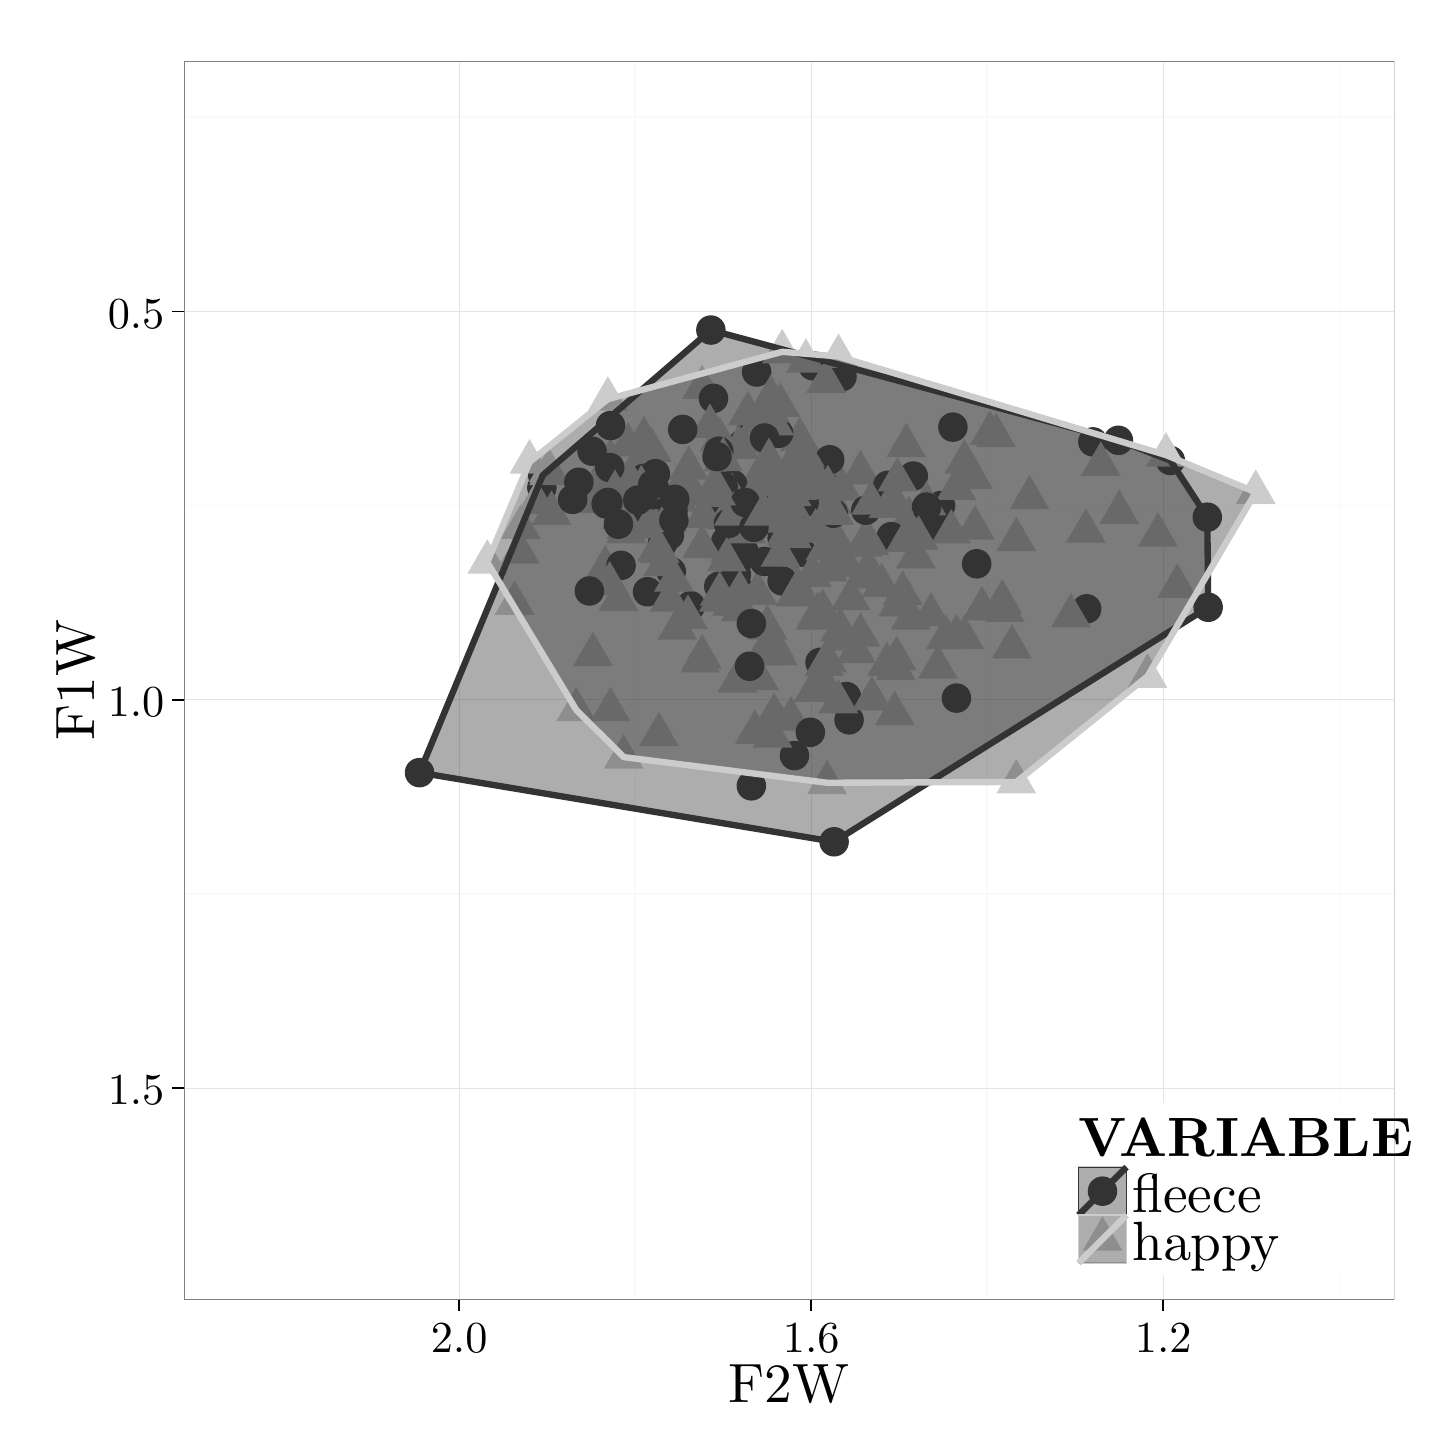
\begin{tikzpicture}[x=1pt,y=1pt]
\definecolor{fillColor}{RGB}{255,255,255}
\path[use as bounding box,fill=fillColor,fill opacity=0.00] (0,0) rectangle (505.89,505.89);
\begin{scope}
\path[clip] (  0.00,  0.00) rectangle (505.89,505.89);
\definecolor{drawColor}{RGB}{255,255,255}
\definecolor{fillColor}{RGB}{255,255,255}

\path[draw=drawColor,line width= 0.6pt,line join=round,line cap=round,fill=fillColor] (  0.00, -0.00) rectangle (505.89,505.89);
\end{scope}
\begin{scope}
\path[clip] ( 56.50, 46.31) rectangle (493.85,493.84);
\definecolor{fillColor}{RGB}{255,255,255}

\path[fill=fillColor] ( 56.50, 46.31) rectangle (493.85,493.84);
\definecolor{drawColor}{gray}{0.98}

\path[draw=drawColor,line width= 0.6pt,line join=round] ( 56.50,473.50) --
	(493.85,473.50);

\path[draw=drawColor,line width= 0.6pt,line join=round] ( 56.50,333.21) --
	(493.85,333.21);

\path[draw=drawColor,line width= 0.6pt,line join=round] ( 56.50,192.91) --
	(493.85,192.91);

\path[draw=drawColor,line width= 0.6pt,line join=round] (473.97, 46.31) --
	(473.97,493.84);

\path[draw=drawColor,line width= 0.6pt,line join=round] (346.74, 46.31) --
	(346.74,493.84);

\path[draw=drawColor,line width= 0.6pt,line join=round] (219.51, 46.31) --
	(219.51,493.84);
\definecolor{drawColor}{gray}{0.90}

\path[draw=drawColor,line width= 0.2pt,line join=round] ( 56.50,403.36) --
	(493.85,403.36);

\path[draw=drawColor,line width= 0.2pt,line join=round] ( 56.50,263.06) --
	(493.85,263.06);

\path[draw=drawColor,line width= 0.2pt,line join=round] ( 56.50,122.77) --
	(493.85,122.77);

\path[draw=drawColor,line width= 0.2pt,line join=round] (410.35, 46.31) --
	(410.35,493.84);

\path[draw=drawColor,line width= 0.2pt,line join=round] (283.13, 46.31) --
	(283.13,493.84);

\path[draw=drawColor,line width= 0.2pt,line join=round] (155.90, 46.31) --
	(155.90,493.84);
\definecolor{fillColor}{gray}{0.80}

\path[fill=fillColor] (302.21,315.69) --
	(309.39,303.25) --
	(295.03,303.25) --
	cycle;
\definecolor{fillColor}{gray}{0.20}

\path[fill=fillColor] (257.68,302.06) circle (  5.33);

\path[fill=fillColor] (258.63,325.91) circle (  5.33);
\definecolor{fillColor}{gray}{0.80}

\path[fill=fillColor] (304.75,316.81) --
	(311.94,304.37) --
	(297.57,304.37) --
	cycle;
\definecolor{fillColor}{gray}{0.20}

\path[fill=fillColor] (263.41,381.47) circle (  5.33);
\definecolor{fillColor}{gray}{0.80}

\path[fill=fillColor] (282.81,340.94) --
	(289.99,328.50) --
	(275.62,328.50) --
	cycle;
\definecolor{fillColor}{gray}{0.20}

\path[fill=fillColor] (294.26,379.79) circle (  5.33);
\definecolor{fillColor}{gray}{0.80}

\path[fill=fillColor] (292.99,395.38) --
	(300.17,382.93) --
	(285.80,382.93) --
	cycle;

\path[fill=fillColor] (278.67,309.80) --
	(285.86,297.35) --
	(271.49,297.35) --
	cycle;

\path[fill=fillColor] (278.99,365.35) --
	(286.18,352.91) --
	(271.81,352.91) --
	cycle;

\path[fill=fillColor] (300.94,353.29) --
	(308.12,340.84) --
	(293.75,340.84) --
	cycle;
\definecolor{fillColor}{gray}{0.20}

\path[fill=fillColor] (283.76,383.71) circle (  5.33);

\path[fill=fillColor] (258.32,355.37) circle (  5.33);

\path[fill=fillColor] (239.55,297.01) circle (  5.33);
\definecolor{fillColor}{gray}{0.80}

\path[fill=fillColor] (301.89,327.19) --
	(309.08,314.75) --
	(294.71,314.75) --
	cycle;

\path[fill=fillColor] (288.53,386.40) --
	(295.72,373.95) --
	(281.35,373.95) --
	cycle;
\definecolor{fillColor}{gray}{0.20}

\path[fill=fillColor] (291.40,211.71) circle (  5.33);
\definecolor{fillColor}{gray}{0.80}

\path[fill=fillColor] (290.76,342.63) --
	(297.94,330.18) --
	(283.57,330.18) --
	cycle;

\path[fill=fillColor] (318.43,336.73) --
	(325.62,324.29) --
	(311.25,324.29) --
	cycle;
\definecolor{fillColor}{gray}{0.20}

\path[fill=fillColor] (261.50,360.14) circle (  5.33);
\definecolor{fillColor}{gray}{0.80}

\path[fill=fillColor] (271.99,377.70) --
	(279.18,365.26) --
	(264.81,365.26) --
	cycle;
\definecolor{fillColor}{gray}{0.20}

\path[fill=fillColor] (272.63,321.42) circle (  5.33);
\definecolor{fillColor}{gray}{0.80}

\path[fill=fillColor] (255.45,312.60) --
	(262.64,300.16) --
	(248.27,300.16) --
	cycle;

\path[fill=fillColor] (277.40,357.78) --
	(284.59,345.33) --
	(270.22,345.33) --
	cycle;

\path[fill=fillColor] (284.40,352.45) --
	(291.58,340.00) --
	(277.21,340.00) --
	cycle;

\path[fill=fillColor] (265.63,367.60) --
	(272.82,355.15) --
	(258.45,355.15) --
	cycle;

\path[fill=fillColor] (281.22,393.69) --
	(288.40,381.25) --
	(274.03,381.25) --
	cycle;
\definecolor{fillColor}{gray}{0.20}

\path[fill=fillColor] (271.36,359.30) circle (  5.33);
\definecolor{fillColor}{gray}{0.80}

\path[fill=fillColor] (297.44,307.83) --
	(304.62,295.39) --
	(290.25,295.39) --
	cycle;

\path[fill=fillColor] (268.18,375.74) --
	(275.36,363.29) --
	(260.99,363.29) --
	cycle;

\path[fill=fillColor] (317.48,363.11) --
	(324.66,350.67) --
	(310.29,350.67) --
	cycle;

\path[fill=fillColor] (338.47,293.80) --
	(345.65,281.36) --
	(331.28,281.36) --
	cycle;

\path[fill=fillColor] (268.81,355.81) --
	(276.00,343.37) --
	(261.63,343.37) --
	cycle;

\path[fill=fillColor] (243.69,384.15) --
	(250.87,371.71) --
	(236.50,371.71) --
	cycle;

\path[fill=fillColor] (260.23,374.61) --
	(267.41,362.17) --
	(253.04,362.17) --
	cycle;

\path[fill=fillColor] (265.95,350.76) --
	(273.14,338.32) --
	(258.77,338.32) --
	cycle;

\path[fill=fillColor] (272.63,397.06) --
	(279.81,384.62) --
	(265.44,384.62) --
	cycle;

\path[fill=fillColor] (265.00,353.29) --
	(272.18,340.84) --
	(257.81,340.84) --
	cycle;

\path[fill=fillColor] (268.49,380.51) --
	(275.68,368.06) --
	(261.31,368.06) --
	cycle;

\path[fill=fillColor] (257.04,362.55) --
	(264.23,350.10) --
	(249.86,350.10) --
	cycle;
\definecolor{fillColor}{gray}{0.20}

\path[fill=fillColor] (249.73,304.03) circle (  5.33);
\definecolor{fillColor}{gray}{0.80}

\path[fill=fillColor] (287.26,354.13) --
	(294.45,341.69) --
	(280.08,341.69) --
	cycle;
\definecolor{fillColor}{gray}{0.20}

\path[fill=fillColor] (246.87,396.62) circle (  5.33);

\path[fill=fillColor] (221.42,328.16) circle (  5.33);

\path[fill=fillColor] (286.31,276.53) circle (  5.33);
\definecolor{fillColor}{gray}{0.80}

\path[fill=fillColor] (291.71,328.88) --
	(298.90,316.43) --
	(284.53,316.43) --
	cycle;

\path[fill=fillColor] (277.08,313.73) --
	(284.27,301.28) --
	(269.90,301.28) --
	cycle;

\path[fill=fillColor] (254.50,305.87) --
	(261.68,293.43) --
	(247.32,293.43) --
	cycle;
\definecolor{fillColor}{gray}{0.20}

\path[fill=fillColor] (266.27,328.16) circle (  5.33);
\definecolor{fillColor}{gray}{0.80}

\path[fill=fillColor] (263.72,309.80) --
	(270.91,297.35) --
	(256.54,297.35) --
	cycle;

\path[fill=fillColor] (310.48,283.98) --
	(317.66,271.54) --
	(303.29,271.54) --
	cycle;
\definecolor{fillColor}{gray}{0.20}

\path[fill=fillColor] (232.55,309.36) circle (  5.33);

\path[fill=fillColor] (296.80,255.77) circle (  5.33);
\definecolor{fillColor}{gray}{0.80}

\path[fill=fillColor] (326.38,301.94) --
	(333.57,289.50) --
	(319.20,289.50) --
	cycle;

\path[fill=fillColor] (265.63,287.91) --
	(272.82,275.47) --
	(258.45,275.47) --
	cycle;
\definecolor{fillColor}{gray}{0.20}

\path[fill=fillColor] (295.85,264.18) circle (  5.33);
\definecolor{fillColor}{gray}{0.80}

\path[fill=fillColor] (331.79,293.80) --
	(338.98,281.36) --
	(324.61,281.36) --
	cycle;

\path[fill=fillColor] (284.72,300.82) --
	(291.90,288.38) --
	(277.53,288.38) --
	cycle;

\path[fill=fillColor] (271.04,287.91) --
	(278.22,275.47) --
	(263.85,275.47) --
	cycle;

\path[fill=fillColor] (249.73,307.27) --
	(256.91,294.83) --
	(242.54,294.83) --
	cycle;
\definecolor{fillColor}{gray}{0.20}

\path[fill=fillColor] (329.88,333.21) circle (  5.33);
\definecolor{fillColor}{gray}{0.80}

\path[fill=fillColor] (285.35,302.22) --
	(292.54,289.78) --
	(278.17,289.78) --
	cycle;
\definecolor{fillColor}{gray}{0.20}

\path[fill=fillColor] (229.37,319.46) circle (  5.33);

\path[fill=fillColor] (312.07,321.98) circle (  5.33);
\definecolor{fillColor}{gray}{0.80}

\path[fill=fillColor] (275.17,330.56) --
	(282.36,318.12) --
	(267.99,318.12) --
	cycle;

\path[fill=fillColor] (253.86,325.51) --
	(261.05,313.07) --
	(246.68,313.07) --
	cycle;
\definecolor{fillColor}{gray}{0.20}

\path[fill=fillColor] (223.97,302.06) circle (  5.33);
\definecolor{fillColor}{gray}{0.80}

\path[fill=fillColor] (289.17,318.22) --
	(296.35,305.77) --
	(281.98,305.77) --
	cycle;

\path[fill=fillColor] (257.68,303.91) --
	(264.87,291.46) --
	(250.50,291.46) --
	cycle;

\path[fill=fillColor] (224.60,339.82) --
	(231.79,327.38) --
	(217.42,327.38) --
	cycle;

\path[fill=fillColor] (320.98,322.99) --
	(328.16,310.54) --
	(313.79,310.54) --
	cycle;
\definecolor{fillColor}{gray}{0.20}

\path[fill=fillColor] (269.13,336.58) circle (  5.33);

\path[fill=fillColor] (310.80,340.50) circle (  5.33);

\path[fill=fillColor] (262.77,330.12) circle (  5.33);
\definecolor{fillColor}{gray}{0.80}

\path[fill=fillColor] (269.77,370.97) --
	(276.95,358.52) --
	(262.58,358.52) --
	cycle;

\path[fill=fillColor] (349.92,366.76) --
	(357.10,354.31) --
	(342.74,354.31) --
	cycle;
\definecolor{fillColor}{gray}{0.20}

\path[fill=fillColor] (289.49,339.10) circle (  5.33);
\definecolor{fillColor}{gray}{0.80}

\path[fill=fillColor] (216.33,333.65) --
	(223.52,321.20) --
	(209.15,321.20) --
	cycle;

\path[fill=fillColor] (319.07,300.82) --
	(326.25,288.38) --
	(311.88,288.38) --
	cycle;
\definecolor{fillColor}{gray}{0.20}

\path[fill=fillColor] (256.09,308.24) circle (  5.33);
\definecolor{fillColor}{gray}{0.80}

\path[fill=fillColor] (300.94,294.65) --
	(308.12,282.20) --
	(293.75,282.20) --
	cycle;
\definecolor{fillColor}{gray}{0.20}

\path[fill=fillColor] (250.68,335.45) circle (  5.33);
\definecolor{fillColor}{gray}{0.80}

\path[fill=fillColor] (231.92,307.27) --
	(239.10,294.83) --
	(224.73,294.83) --
	cycle;

\path[fill=fillColor] (278.99,361.15) --
	(286.18,348.70) --
	(271.81,348.70) --
	cycle;

\path[fill=fillColor] (233.51,314.57) --
	(240.69,302.12) --
	(226.32,302.12) --
	cycle;

\path[fill=fillColor] (262.77,259.57) --
	(269.95,247.13) --
	(255.58,247.13) --
	cycle;

\path[fill=fillColor] (277.72,323.55) --
	(284.90,311.10) --
	(270.53,311.10) --
	cycle;

\path[fill=fillColor] (267.22,297.45) --
	(274.41,285.01) --
	(260.04,285.01) --
	cycle;

\path[fill=fillColor] (317.16,328.88) --
	(324.34,316.43) --
	(309.97,316.43) --
	cycle;

\path[fill=fillColor] (252.27,337.02) --
	(259.46,324.57) --
	(245.09,324.57) --
	cycle;

\path[fill=fillColor] (285.67,353.85) --
	(292.86,341.41) --
	(278.49,341.41) --
	cycle;

\path[fill=fillColor] (292.67,327.76) --
	(299.85,315.31) --
	(285.48,315.31) --
	cycle;

\path[fill=fillColor] (218.56,353.01) --
	(225.74,340.56) --
	(211.37,340.56) --
	cycle;

\path[fill=fillColor] (259.91,364.51) --
	(267.09,352.07) --
	(252.72,352.07) --
	cycle;

\path[fill=fillColor] (277.40,354.97) --
	(284.59,342.53) --
	(270.22,342.53) --
	cycle;

\path[fill=fillColor] (225.56,361.43) --
	(232.74,348.98) --
	(218.37,348.98) --
	cycle;

\path[fill=fillColor] (265.95,335.89) --
	(273.14,323.45) --
	(258.77,323.45) --
	cycle;

\path[fill=fillColor] (234.78,343.47) --
	(241.96,331.02) --
	(227.59,331.02) --
	cycle;

\path[fill=fillColor] (264.36,368.72) --
	(271.54,356.28) --
	(257.18,356.28) --
	cycle;
\definecolor{fillColor}{gray}{0.20}

\path[fill=fillColor] (252.27,320.30) circle (  5.33);
\definecolor{fillColor}{gray}{0.80}

\path[fill=fillColor] (210.61,357.50) --
	(217.79,345.05) --
	(203.42,345.05) --
	cycle;
\definecolor{fillColor}{gray}{0.20}

\path[fill=fillColor] (233.19,331.24) circle (  5.33);
\definecolor{fillColor}{gray}{0.80}

\path[fill=fillColor] (287.90,276.69) --
	(295.08,264.24) --
	(280.71,264.24) --
	cycle;
\definecolor{fillColor}{gray}{0.20}

\path[fill=fillColor] (256.73,313.29) circle (  5.33);

\path[fill=fillColor] (247.82,371.93) circle (  5.33);
\definecolor{fillColor}{gray}{0.80}

\path[fill=fillColor] (262.45,346.56) --
	(269.64,334.11) --
	(255.27,334.11) --
	cycle;
\definecolor{fillColor}{gray}{0.20}

\path[fill=fillColor] (277.08,242.86) circle (  5.33);
\definecolor{fillColor}{gray}{0.80}

\path[fill=fillColor] (269.77,265.75) --
	(276.95,253.30) --
	(262.58,253.30) --
	cycle;
\definecolor{fillColor}{gray}{0.20}

\path[fill=fillColor] (220.47,332.65) circle (  5.33);
\definecolor{fillColor}{gray}{0.80}

\path[fill=fillColor] (287.90,283.98) --
	(295.08,271.54) --
	(280.71,271.54) --
	cycle;

\path[fill=fillColor] (299.35,288.75) --
	(306.53,276.31) --
	(292.16,276.31) --
	cycle;

\path[fill=fillColor] (284.08,274.73) --
	(291.27,262.28) --
	(276.90,262.28) --
	cycle;

\path[fill=fillColor] (259.59,339.54) --
	(266.77,327.10) --
	(252.40,327.10) --
	cycle;
\definecolor{fillColor}{gray}{0.20}

\path[fill=fillColor] (272.63,305.99) circle (  5.33);

\path[fill=fillColor] (254.82,340.78) circle (  5.33);

\path[fill=fillColor] (279.63,316.37) circle (  5.33);
\definecolor{fillColor}{gray}{0.80}

\path[fill=fillColor] (266.27,374.33) --
	(273.45,361.89) --
	(259.08,361.89) --
	cycle;

\path[fill=fillColor] (280.26,350.76) --
	(287.45,338.32) --
	(273.08,338.32) --
	cycle;
\definecolor{fillColor}{gray}{0.20}

\path[fill=fillColor] (291.08,330.40) circle (  5.33);
\definecolor{fillColor}{gray}{0.80}

\path[fill=fillColor] (316.20,309.80) --
	(323.39,297.35) --
	(309.02,297.35) --
	cycle;

\path[fill=fillColor] (313.98,286.23) --
	(321.16,273.78) --
	(306.79,273.78) --
	cycle;
\definecolor{fillColor}{gray}{0.20}

\path[fill=fillColor] (258.95,316.37) circle (  5.33);
\definecolor{fillColor}{gray}{0.80}

\path[fill=fillColor] (288.85,285.39) --
	(296.04,272.94) --
	(281.67,272.94) --
	cycle;
\definecolor{fillColor}{gray}{0.20}

\path[fill=fillColor] (266.27,357.62) circle (  5.33);
\definecolor{fillColor}{gray}{0.80}

\path[fill=fillColor] (277.40,309.24) --
	(284.59,296.79) --
	(270.22,296.79) --
	cycle;

\path[fill=fillColor] (288.85,339.82) --
	(296.04,327.38) --
	(281.67,327.38) --
	cycle;

\path[fill=fillColor] (266.27,351.89) --
	(273.45,339.44) --
	(259.08,339.44) --
	cycle;

\path[fill=fillColor] (244.32,337.58) --
	(251.51,325.13) --
	(237.14,325.13) --
	cycle;

\path[fill=fillColor] (254.50,345.15) --
	(261.68,332.71) --
	(247.32,332.71) --
	cycle;

\path[fill=fillColor] (313.34,266.31) --
	(320.53,253.86) --
	(306.16,253.86) --
	cycle;

\path[fill=fillColor] (250.05,365.35) --
	(257.23,352.91) --
	(242.86,352.91) --
	cycle;
\definecolor{fillColor}{gray}{0.20}

\path[fill=fillColor] (251.32,340.22) circle (  5.33);
\definecolor{fillColor}{gray}{0.80}

\path[fill=fillColor] (275.81,264.34) --
	(283.00,251.90) --
	(268.63,251.90) --
	cycle;

\path[fill=fillColor] (294.26,347.40) --
	(301.44,334.95) --
	(287.07,334.95) --
	cycle;

\path[fill=fillColor] (279.95,352.45) --
	(287.13,340.00) --
	(272.76,340.00) --
	cycle;

\path[fill=fillColor] (264.36,278.93) --
	(271.54,266.49) --
	(257.18,266.49) --
	cycle;

\path[fill=fillColor] (214.74,337.30) --
	(221.93,324.85) --
	(207.56,324.85) --
	cycle;

\path[fill=fillColor] (216.97,363.39) --
	(224.15,350.95) --
	(209.78,350.95) --
	cycle;

\path[fill=fillColor] (205.84,347.96) --
	(213.02,335.51) --
	(198.65,335.51) --
	cycle;

\path[fill=fillColor] (222.69,365.64) --
	(229.88,353.19) --
	(215.51,353.19) --
	cycle;

\path[fill=fillColor] (223.01,352.45) --
	(230.20,340.00) --
	(215.83,340.00) --
	cycle;

\path[fill=fillColor] (224.28,333.93) --
	(231.47,321.48) --
	(217.10,321.48) --
	cycle;

\path[fill=fillColor] (240.51,345.43) --
	(247.69,332.99) --
	(233.32,332.99) --
	cycle;

\path[fill=fillColor] (236.05,348.52) --
	(243.24,336.08) --
	(228.87,336.08) --
	cycle;

\path[fill=fillColor] (209.65,379.95) --
	(216.84,367.50) --
	(202.47,367.50) --
	cycle;
\definecolor{fillColor}{gray}{0.20}

\path[fill=fillColor] (226.83,344.71) circle (  5.33);
\definecolor{fillColor}{gray}{0.80}

\path[fill=fillColor] (246.55,370.12) --
	(253.73,357.68) --
	(239.36,357.68) --
	cycle;
\definecolor{fillColor}{gray}{0.20}

\path[fill=fillColor] (249.73,352.85) circle (  5.33);

\path[fill=fillColor] (231.92,322.55) circle (  5.33);

\path[fill=fillColor] (384.91,356.22) circle (  5.33);
\definecolor{fillColor}{gray}{0.80}

\path[fill=fillColor] (275.49,337.30) --
	(282.68,324.85) --
	(268.31,324.85) --
	cycle;
\definecolor{fillColor}{gray}{0.20}

\path[fill=fillColor] (327.97,325.07) circle (  5.33);
\definecolor{fillColor}{gray}{0.80}

\path[fill=fillColor] (259.59,331.96) --
	(266.77,319.52) --
	(252.40,319.52) --
	cycle;

\path[fill=fillColor] (283.44,316.25) --
	(290.63,303.81) --
	(276.26,303.81) --
	cycle;

\path[fill=fillColor] (362.01,344.31) --
	(369.19,331.87) --
	(354.82,331.87) --
	cycle;

\path[fill=fillColor] (357.24,329.16) --
	(364.42,316.71) --
	(350.05,316.71) --
	cycle;
\definecolor{fillColor}{gray}{0.20}

\path[fill=fillColor] (185.80,339.66) circle (  5.33);

\path[fill=fillColor] (226.51,339.38) circle (  5.33);

\path[fill=fillColor] (269.77,332.09) circle (  5.33);
\definecolor{fillColor}{gray}{0.80}

\path[fill=fillColor] (279.63,336.73) --
	(286.81,324.29) --
	(272.44,324.29) --
	cycle;

\path[fill=fillColor] (313.66,282.58) --
	(320.85,270.14) --
	(306.48,270.14) --
	cycle;
\definecolor{fillColor}{gray}{0.20}

\path[fill=fillColor] (226.19,337.14) circle (  5.33);
\definecolor{fillColor}{gray}{0.80}

\path[fill=fillColor] (274.54,343.75) --
	(281.72,331.31) --
	(267.35,331.31) --
	cycle;

\path[fill=fillColor] (285.99,347.40) --
	(293.17,334.95) --
	(278.80,334.95) --
	cycle;
\definecolor{fillColor}{gray}{0.20}

\path[fill=fillColor] (282.81,251.28) circle (  5.33);
\definecolor{fillColor}{gray}{0.80}

\path[fill=fillColor] (292.99,270.52) --
	(300.17,258.07) --
	(285.80,258.07) --
	cycle;
\definecolor{fillColor}{gray}{0.20}

\path[fill=fillColor] (266.27,313.01) circle (  5.33);
\definecolor{fillColor}{gray}{0.80}

\path[fill=fillColor] (293.62,296.61) --
	(300.81,284.17) --
	(286.44,284.17) --
	cycle;

\path[fill=fillColor] (287.58,338.98) --
	(294.76,326.54) --
	(280.39,326.54) --
	cycle;

\path[fill=fillColor] (333.70,331.96) --
	(340.88,319.52) --
	(326.51,319.52) --
	cycle;

\path[fill=fillColor] (228.42,324.95) --
	(235.60,312.51) --
	(221.23,312.51) --
	cycle;

\path[fill=fillColor] (314.61,305.59) --
	(321.80,293.15) --
	(307.43,293.15) --
	cycle;

\path[fill=fillColor] (335.61,294.09) --
	(342.79,281.64) --
	(328.42,281.64) --
	cycle;

\path[fill=fillColor] (238.60,301.10) --
	(245.78,288.66) --
	(231.41,288.66) --
	cycle;

\path[fill=fillColor] (341.65,351.61) --
	(348.84,339.16) --
	(334.47,339.16) --
	cycle;

\path[fill=fillColor] (243.69,326.63) --
	(250.87,314.19) --
	(236.50,314.19) --
	cycle;

\path[fill=fillColor] (328.93,283.14) --
	(336.11,270.70) --
	(321.74,270.70) --
	cycle;

\path[fill=fillColor] (288.85,241.34) --
	(296.04,228.89) --
	(281.67,228.89) --
	cycle;

\path[fill=fillColor] (216.33,331.96) --
	(223.52,319.52) --
	(209.15,319.52) --
	cycle;

\path[fill=fillColor] (308.57,312.60) --
	(315.76,300.16) --
	(301.39,300.16) --
	cycle;

\path[fill=fillColor] (267.22,297.17) --
	(274.41,284.73) --
	(260.04,284.73) --
	cycle;

\path[fill=fillColor] (287.26,303.34) --
	(294.45,290.90) --
	(280.08,290.90) --
	cycle;

\path[fill=fillColor] (288.22,325.79) --
	(295.40,313.35) --
	(281.03,313.35) --
	cycle;

\path[fill=fillColor] (295.85,319.90) --
	(303.03,307.46) --
	(288.66,307.46) --
	cycle;

\path[fill=fillColor] (279.31,334.21) --
	(286.49,321.77) --
	(272.12,321.77) --
	cycle;

\path[fill=fillColor] (251.32,358.06) --
	(258.50,345.61) --
	(244.13,345.61) --
	cycle;

\path[fill=fillColor] (257.36,310.08) --
	(264.55,297.63) --
	(250.18,297.63) --
	cycle;
\definecolor{fillColor}{gray}{0.20}

\path[fill=fillColor] (289.81,349.76) circle (  5.33);
\definecolor{fillColor}{gray}{0.80}

\path[fill=fillColor] (189.30,338.70) --
	(196.48,326.25) --
	(182.11,326.25) --
	cycle;
\definecolor{fillColor}{gray}{0.20}

\path[fill=fillColor] (186.12,344.15) circle (  5.33);

\path[fill=fillColor] (253.23,326.75) circle (  5.33);
\definecolor{fillColor}{gray}{0.80}

\path[fill=fillColor] (357.24,241.62) --
	(364.42,229.17) --
	(350.05,229.17) --
	cycle;
\definecolor{fillColor}{gray}{0.20}

\path[fill=fillColor] (426.26,329.00) circle (  5.33);
\definecolor{fillColor}{gray}{0.80}

\path[fill=fillColor] (178.16,333.65) --
	(185.35,321.20) --
	(170.98,321.20) --
	cycle;

\path[fill=fillColor] (243.69,286.79) --
	(250.87,274.35) --
	(236.50,274.35) --
	cycle;

\path[fill=fillColor] (304.12,327.76) --
	(311.30,315.31) --
	(296.93,315.31) --
	cycle;

\path[fill=fillColor] (166.08,321.02) --
	(173.26,308.58) --
	(158.89,308.58) --
	cycle;
\definecolor{fillColor}{gray}{0.20}

\path[fill=fillColor] (141.59,236.69) circle (  5.33);

\path[fill=fillColor] (280.58,334.33) circle (  5.33);

\path[fill=fillColor] (335.61,263.62) circle (  5.33);

\path[fill=fillColor] (276.76,334.89) circle (  5.33);
\definecolor{fillColor}{gray}{0.80}

\path[fill=fillColor] (270.09,290.16) --
	(277.27,277.71) --
	(262.90,277.71) --
	cycle;
\definecolor{fillColor}{gray}{0.20}

\path[fill=fillColor] (412.90,349.48) circle (  5.33);
\definecolor{fillColor}{gray}{0.80}

\path[fill=fillColor] (342.29,333.37) --
	(349.47,320.92) --
	(335.10,320.92) --
	cycle;
\definecolor{fillColor}{gray}{0.20}

\path[fill=fillColor] (320.02,343.87) circle (  5.33);
\definecolor{fillColor}{gray}{0.80}

\path[fill=fillColor] (352.15,306.71) --
	(359.33,294.27) --
	(344.96,294.27) --
	cycle;

\path[fill=fillColor] (335.61,347.68) --
	(342.79,335.23) --
	(328.42,335.23) --
	cycle;

\path[fill=fillColor] (175.94,306.15) --
	(183.12,293.71) --
	(168.75,293.71) --
	cycle;

\path[fill=fillColor] (256.41,278.09) --
	(263.59,265.65) --
	(249.22,265.65) --
	cycle;
\definecolor{fillColor}{gray}{0.20}

\path[fill=fillColor] (394.13,356.78) circle (  5.33);
\definecolor{fillColor}{gray}{0.80}

\path[fill=fillColor] (215.38,250.59) --
	(222.56,238.15) --
	(208.19,238.15) --
	cycle;

\path[fill=fillColor] (387.77,356.38) --
	(394.95,343.93) --
	(380.58,343.93) --
	cycle;

\path[fill=fillColor] (411.31,359.74) --
	(418.49,347.30) --
	(404.12,347.30) --
	cycle;

\path[fill=fillColor] (229.69,320.18) --
	(236.88,307.74) --
	(222.51,307.74) --
	cycle;
\definecolor{fillColor}{gray}{0.20}

\path[fill=fillColor] (382.68,295.89) circle (  5.33);

\path[fill=fillColor] (210.61,362.11) circle (  5.33);
\definecolor{fillColor}{gray}{0.80}

\path[fill=fillColor] (234.78,297.17) --
	(241.96,284.73) --
	(227.59,284.73) --
	cycle;
\definecolor{fillColor}{gray}{0.20}

\path[fill=fillColor] (342.92,312.16) circle (  5.33);

\path[fill=fillColor] (260.86,275.13) circle (  5.33);
\definecolor{fillColor}{gray}{0.80}

\path[fill=fillColor] (275.49,341.50) --
	(282.68,329.06) --
	(268.31,329.06) --
	cycle;
\definecolor{fillColor}{gray}{0.20}

\path[fill=fillColor] (222.69,343.03) circle (  5.33);
\definecolor{fillColor}{gray}{0.80}

\path[fill=fillColor] (208.70,319.06) --
	(215.88,306.61) --
	(201.51,306.61) --
	cycle;
\definecolor{fillColor}{gray}{0.20}

\path[fill=fillColor] (302.85,331.52) circle (  5.33);
\definecolor{fillColor}{gray}{0.80}

\path[fill=fillColor] (271.99,323.55) --
	(279.18,311.10) --
	(264.81,311.10) --
	cycle;

\path[fill=fillColor] (200.75,342.91) --
	(207.93,330.46) --
	(193.56,330.46) --
	cycle;

\path[fill=fillColor] (267.22,352.73) --
	(274.41,340.28) --
	(260.04,340.28) --
	cycle;

\path[fill=fillColor] (267.86,357.78) --
	(275.04,345.33) --
	(260.67,345.33) --
	cycle;
\definecolor{fillColor}{gray}{0.20}

\path[fill=fillColor] (210.29,346.96) circle (  5.33);

\path[fill=fillColor] (203.93,352.85) circle (  5.33);

\path[fill=fillColor] (214.42,311.60) circle (  5.33);
\definecolor{fillColor}{gray}{0.80}

\path[fill=fillColor] (213.47,307.55) --
	(220.65,295.11) --
	(206.28,295.11) --
	cycle;
\definecolor{fillColor}{gray}{0.20}

\path[fill=fillColor] (213.47,326.47) circle (  5.33);
\definecolor{fillColor}{gray}{0.80}

\path[fill=fillColor] (255.14,338.42) --
	(262.32,325.97) --
	(247.95,325.97) --
	cycle;

\path[fill=fillColor] (355.65,290.44) --
	(362.83,277.99) --
	(348.46,277.99) --
	cycle;
\definecolor{fillColor}{gray}{0.20}

\path[fill=fillColor] (426.57,296.45) circle (  5.33);
\definecolor{fillColor}{gray}{0.80}

\path[fill=fillColor] (228.10,258.73) --
	(235.29,246.29) --
	(220.92,246.29) --
	cycle;
\definecolor{fillColor}{gray}{0.20}

\path[fill=fillColor] (261.50,290.56) circle (  5.33);
\definecolor{fillColor}{gray}{0.80}

\path[fill=fillColor] (243.05,285.39) --
	(250.23,272.94) --
	(235.86,272.94) --
	cycle;

\path[fill=fillColor] (267.22,349.08) --
	(274.41,336.64) --
	(260.04,336.64) --
	cycle;

\path[fill=fillColor] (324.79,342.07) --
	(331.98,329.62) --
	(317.61,329.62) --
	cycle;

\path[fill=fillColor] (188.34,353.01) --
	(195.53,340.56) --
	(181.16,340.56) --
	cycle;

\path[fill=fillColor] (210.29,313.17) --
	(217.47,300.72) --
	(203.10,300.72) --
	cycle;
\definecolor{fillColor}{gray}{0.20}

\path[fill=fillColor] (196.93,335.45) circle (  5.33);
\definecolor{fillColor}{gray}{0.80}

\path[fill=fillColor] (227.46,325.51) --
	(234.65,313.07) --
	(220.28,313.07) --
	cycle;

\path[fill=fillColor] (276.13,330.28) --
	(283.31,317.84) --
	(268.94,317.84) --
	cycle;

\path[fill=fillColor] (276.13,345.43) --
	(283.31,332.99) --
	(268.94,332.99) --
	cycle;

\path[fill=fillColor] (218.56,348.80) --
	(225.74,336.36) --
	(211.37,336.36) --
	cycle;

\path[fill=fillColor] (210.61,267.71) --
	(217.79,255.27) --
	(203.42,255.27) --
	cycle;

\path[fill=fillColor] (347.69,367.60) --
	(354.88,355.15) --
	(340.51,355.15) --
	cycle;

\path[fill=fillColor] (221.74,347.96) --
	(228.92,335.51) --
	(214.55,335.51) --
	cycle;

\path[fill=fillColor] (188.34,354.13) --
	(195.53,341.69) --
	(181.16,341.69) --
	cycle;

\path[fill=fillColor] (177.85,324.67) --
	(185.03,312.23) --
	(170.66,312.23) --
	cycle;

\path[fill=fillColor] (230.96,336.17) --
	(238.15,323.73) --
	(223.78,323.73) --
	cycle;

\path[fill=fillColor] (248.46,348.52) --
	(255.64,336.08) --
	(241.27,336.08) --
	cycle;

\path[fill=fillColor] (212.20,346.27) --
	(219.38,333.83) --
	(205.01,333.83) --
	cycle;

\path[fill=fillColor] (181.34,357.22) --
	(188.53,344.77) --
	(174.16,344.77) --
	cycle;
\definecolor{fillColor}{gray}{0.20}

\path[fill=fillColor] (233.51,327.88) circle (  5.33);
\definecolor{fillColor}{gray}{0.80}

\path[fill=fillColor] (238.91,354.97) --
	(246.10,342.53) --
	(231.73,342.53) --
	cycle;
\definecolor{fillColor}{gray}{0.20}

\path[fill=fillColor] (199.16,341.63) circle (  5.33);
\definecolor{fillColor}{gray}{0.80}

\path[fill=fillColor] (278.04,347.68) --
	(285.22,335.23) --
	(270.85,335.23) --
	cycle;
\definecolor{fillColor}{gray}{0.20}

\path[fill=fillColor] (261.50,231.92) circle (  5.33);

\path[fill=fillColor] (202.97,302.34) circle (  5.33);

\path[fill=fillColor] (220.47,335.17) circle (  5.33);
\definecolor{fillColor}{gray}{0.80}

\path[fill=fillColor] (338.47,357.22) --
	(345.65,344.77) --
	(331.28,344.77) --
	cycle;
\definecolor{fillColor}{gray}{0.20}

\path[fill=fillColor] (233.83,335.45) circle (  5.33);
\definecolor{fillColor}{gray}{0.80}

\path[fill=fillColor] (274.22,331.40) --
	(281.40,318.96) --
	(267.04,318.96) --
	cycle;

\path[fill=fillColor] (269.13,258.17) --
	(276.32,245.73) --
	(261.95,245.73) --
	cycle;

\path[fill=fillColor] (314.30,350.76) --
	(321.48,338.32) --
	(307.11,338.32) --
	cycle;

\path[fill=fillColor] (284.72,332.25) --
	(291.90,319.80) --
	(277.53,319.80) --
	cycle;

\path[fill=fillColor] (415.44,312.32) --
	(422.63,299.88) --
	(408.26,299.88) --
	cycle;
\definecolor{fillColor}{gray}{0.20}

\path[fill=fillColor] (225.87,340.78) circle (  5.33);

\path[fill=fillColor] (209.65,334.33) circle (  5.33);

\path[fill=fillColor] (324.79,332.65) circle (  5.33);
\definecolor{fillColor}{gray}{0.80}

\path[fill=fillColor] (280.90,359.46) --
	(288.08,347.02) --
	(273.71,347.02) --
	cycle;

\path[fill=fillColor] (250.05,309.52) --
	(257.23,297.07) --
	(242.86,297.07) --
	cycle;

\path[fill=fillColor] (443.75,346.27) --
	(450.93,333.83) --
	(436.56,333.83) --
	cycle;
\definecolor{fillColor}{gray}{0.20}

\path[fill=fillColor] (249.09,350.89) circle (  5.33);
\definecolor{fillColor}{gray}{0.80}

\path[fill=fillColor] (289.17,347.96) --
	(296.35,335.51) --
	(281.98,335.51) --
	cycle;

\path[fill=fillColor] (291.40,338.70) --
	(298.58,326.25) --
	(284.21,326.25) --
	cycle;
\definecolor{fillColor}{gray}{0.20}

\path[fill=fillColor] (334.33,361.55) circle (  5.33);
\definecolor{fillColor}{gray}{0.80}

\path[fill=fillColor] (376.96,301.66) --
	(384.14,289.22) --
	(369.77,289.22) --
	cycle;
\definecolor{fillColor}{gray}{0.20}

\path[fill=fillColor] (259.27,334.33) circle (  5.33);
\definecolor{fillColor}{gray}{0.80}

\path[fill=fillColor] (293.62,293.24) --
	(300.81,280.80) --
	(286.44,280.80) --
	cycle;

\path[fill=fillColor] (269.77,340.10) --
	(276.95,327.66) --
	(262.58,327.66) --
	cycle;

\path[fill=fillColor] (311.12,341.22) --
	(318.30,328.78) --
	(303.93,328.78) --
	cycle;

\path[fill=fillColor] (321.93,329.72) --
	(329.11,317.28) --
	(314.75,317.28) --
	cycle;

\path[fill=fillColor] (198.20,267.71) --
	(205.39,255.27) --
	(191.02,255.27) --
	cycle;
\definecolor{fillColor}{gray}{0.20}

\path[fill=fillColor] (262.45,325.35) circle (  5.33);
\definecolor{fillColor}{gray}{0.80}

\path[fill=fillColor] (305.07,271.64) --
	(312.26,259.19) --
	(297.89,259.19) --
	cycle;

\path[fill=fillColor] (285.67,350.20) --
	(292.86,337.76) --
	(278.49,337.76) --
	cycle;

\path[fill=fillColor] (252.59,321.86) --
	(259.78,309.42) --
	(245.41,309.42) --
	cycle;

\path[fill=fillColor] (344.83,304.19) --
	(352.02,291.74) --
	(337.65,291.74) --
	cycle;

\path[fill=fillColor] (408.44,330.84) --
	(415.63,318.40) --
	(401.26,318.40) --
	cycle;

\path[fill=fillColor] (248.77,345.71) --
	(255.96,333.27) --
	(241.59,333.27) --
	cycle;

\path[fill=fillColor] (353.10,303.63) --
	(360.29,291.18) --
	(345.92,291.18) --
	cycle;

\path[fill=fillColor] (382.36,332.25) --
	(389.55,319.80) --
	(375.18,319.80) --
	cycle;

\path[fill=fillColor] (394.45,338.98) --
	(401.63,326.54) --
	(387.26,326.54) --
	cycle;

\path[fill=fillColor] (404.63,279.78) --
	(411.81,267.33) --
	(397.44,267.33) --
	cycle;

\path[fill=fillColor] (313.02,342.91) --
	(320.21,330.46) --
	(305.84,330.46) --
	cycle;

\path[fill=fillColor] (304.75,342.35) --
	(311.94,329.90) --
	(297.57,329.90) --
	cycle;

\path[fill=fillColor] (265.95,338.42) --
	(273.14,325.97) --
	(258.77,325.97) --
	cycle;

\path[fill=fillColor] (204.25,287.63) --
	(211.43,275.19) --
	(197.06,275.19) --
	cycle;
\definecolor{fillColor}{gray}{0.20}

\path[fill=fillColor] (209.02,333.77) circle (  5.33);
\definecolor{fillColor}{gray}{0.80}

\path[fill=fillColor] (183.89,342.63) --
	(191.07,330.18) --
	(176.70,330.18) --
	cycle;
\definecolor{fillColor}{gray}{0.20}

\path[fill=fillColor] (236.69,360.71) circle (  5.33);
\definecolor{drawColor}{gray}{0.20}
\definecolor{fillColor}{RGB}{51,51,51}

\path[draw=drawColor,line width= 2.3pt,line join=round,line cap=round,fill=fillColor,fill opacity=0.40] (186.12,344.15) --
	(246.87,396.62) --
	(394.13,356.78) --
	(412.90,349.48) --
	(426.26,329.00) --
	(426.57,296.45) --
	(291.40,211.71) --
	(141.59,236.69) --
	cycle;
\definecolor{drawColor}{gray}{0.80}

\path[draw=drawColor,line width= 2.3pt,line join=round,line cap=round,fill=fillColor,fill opacity=0.40] (166.08,312.73) --
	(181.34,348.92) --
	(209.65,371.65) --
	(272.63,388.76) --
	(292.99,387.08) --
	(411.31,351.45) --
	(443.75,337.98) --
	(404.63,271.48) --
	(357.24,233.32) --
	(288.85,233.04) --
	(215.38,242.30) --
	(198.20,259.41) --
	cycle;
\definecolor{drawColor}{gray}{0.50}

\path[draw=drawColor,line width= 0.6pt,line join=round,line cap=round] ( 56.50, 46.31) rectangle (493.85,493.84);
\end{scope}
\begin{scope}
\path[clip] (  0.00,  0.00) rectangle (505.89,505.89);
\definecolor{drawColor}{RGB}{0,0,0}

\node[text=drawColor,anchor=base east,inner sep=0pt, outer sep=0pt, scale=  1.60] at ( 49.39,397.32) {0.5};

\node[text=drawColor,anchor=base east,inner sep=0pt, outer sep=0pt, scale=  1.60] at ( 49.39,257.03) {1.0};

\node[text=drawColor,anchor=base east,inner sep=0pt, outer sep=0pt, scale=  1.60] at ( 49.39,116.73) {1.5};
\end{scope}
\begin{scope}
\path[clip] (  0.00,  0.00) rectangle (505.89,505.89);
\definecolor{drawColor}{RGB}{0,0,0}

\path[draw=drawColor,line width= 0.6pt,line join=round] ( 52.24,403.36) --
	( 56.50,403.36);

\path[draw=drawColor,line width= 0.6pt,line join=round] ( 52.24,263.06) --
	( 56.50,263.06);

\path[draw=drawColor,line width= 0.6pt,line join=round] ( 52.24,122.77) --
	( 56.50,122.77);
\end{scope}
\begin{scope}
\path[clip] (  0.00,  0.00) rectangle (505.89,505.89);
\definecolor{drawColor}{RGB}{0,0,0}

\path[draw=drawColor,line width= 0.6pt,line join=round] (410.35, 42.04) --
	(410.35, 46.31);

\path[draw=drawColor,line width= 0.6pt,line join=round] (283.13, 42.04) --
	(283.13, 46.31);

\path[draw=drawColor,line width= 0.6pt,line join=round] (155.90, 42.04) --
	(155.90, 46.31);
\end{scope}
\begin{scope}
\path[clip] (  0.00,  0.00) rectangle (505.89,505.89);
\definecolor{drawColor}{RGB}{0,0,0}

\node[text=drawColor,anchor=base,inner sep=0pt, outer sep=0pt, scale=  1.60] at (410.35, 27.13) {1.2};

\node[text=drawColor,anchor=base,inner sep=0pt, outer sep=0pt, scale=  1.60] at (283.13, 27.13) {1.6};

\node[text=drawColor,anchor=base,inner sep=0pt, outer sep=0pt, scale=  1.60] at (155.90, 27.13) {2.0};
\end{scope}
\begin{scope}
\path[clip] (  0.00,  0.00) rectangle (505.89,505.89);
\definecolor{drawColor}{RGB}{0,0,0}

\node[text=drawColor,anchor=base,inner sep=0pt, outer sep=0pt, scale=  2.00] at (275.17,  9.03) {F2W};
\end{scope}
\begin{scope}
\path[clip] (  0.00,  0.00) rectangle (505.89,505.89);
\definecolor{drawColor}{RGB}{0,0,0}

\node[text=drawColor,rotate= 90.00,anchor=base,inner sep=0pt, outer sep=0pt, scale=  2.00] at ( 24.12,270.08) {F1W};
\end{scope}
\begin{scope}
\path[clip] (  0.00,  0.00) rectangle (505.89,505.89);
\definecolor{fillColor}{RGB}{255,255,255}

\path[fill=fillColor] (375.44, 55.18) rectangle (484.98,117.15);
\end{scope}
\begin{scope}
\path[clip] (  0.00,  0.00) rectangle (505.89,505.89);
\definecolor{drawColor}{RGB}{0,0,0}

\node[text=drawColor,anchor=base west,inner sep=0pt, outer sep=0pt, scale=  2.00] at (379.71, 98.13) {\bfseries VARIABLE};
\end{scope}
\begin{scope}
\path[clip] (  0.00,  0.00) rectangle (505.89,505.89);
\definecolor{drawColor}{gray}{0.80}
\definecolor{fillColor}{RGB}{255,255,255}

\path[draw=drawColor,line width= 0.6pt,line join=round,line cap=round,fill=fillColor] (379.71, 76.79) rectangle (397.06, 94.13);
\end{scope}
\begin{scope}
\path[clip] (  0.00,  0.00) rectangle (505.89,505.89);
\definecolor{fillColor}{gray}{0.20}

\path[fill=fillColor] (388.38, 85.46) circle (  5.33);
\end{scope}
\begin{scope}
\path[clip] (  0.00,  0.00) rectangle (505.89,505.89);
\definecolor{drawColor}{gray}{0.20}
\definecolor{fillColor}{RGB}{51,51,51}

\path[draw=drawColor,line width= 0.4pt,line join=round,line cap=round,fill=fillColor,fill opacity=0.40] (379.71, 76.79) rectangle (397.06, 94.13);

\path[draw=drawColor,line width= 2.3pt,line join=round] (379.71, 76.79) --
	(397.06, 94.13);
\end{scope}
\begin{scope}
\path[clip] (  0.00,  0.00) rectangle (505.89,505.89);
\definecolor{drawColor}{gray}{0.80}
\definecolor{fillColor}{RGB}{255,255,255}

\path[draw=drawColor,line width= 0.6pt,line join=round,line cap=round,fill=fillColor] (379.71, 59.44) rectangle (397.06, 76.79);
\end{scope}
\begin{scope}
\path[clip] (  0.00,  0.00) rectangle (505.89,505.89);
\definecolor{fillColor}{gray}{0.80}

\path[fill=fillColor] (388.38, 76.41) --
	(395.57, 63.97) --
	(381.20, 63.97) --
	cycle;
\end{scope}
\begin{scope}
\path[clip] (  0.00,  0.00) rectangle (505.89,505.89);
\definecolor{drawColor}{gray}{0.80}
\definecolor{fillColor}{RGB}{51,51,51}

\path[draw=drawColor,line width= 0.4pt,line join=round,line cap=round,fill=fillColor,fill opacity=0.40] (379.71, 59.44) rectangle (397.06, 76.79);

\path[draw=drawColor,line width= 2.3pt,line join=round] (379.71, 59.44) --
	(397.06, 76.79);
\end{scope}
\begin{scope}
\path[clip] (  0.00,  0.00) rectangle (505.89,505.89);
\definecolor{drawColor}{RGB}{0,0,0}

\node[text=drawColor,anchor=base west,inner sep=0pt, outer sep=0pt, scale=  2.00] at (399.22, 77.92) {fleece};
\end{scope}
\begin{scope}
\path[clip] (  0.00,  0.00) rectangle (505.89,505.89);
\definecolor{drawColor}{RGB}{0,0,0}

\node[text=drawColor,anchor=base west,inner sep=0pt, outer sep=0pt, scale=  2.00] at (399.22, 60.57) {happy};
\end{scope}
\end{tikzpicture}
} 
		\caption{young speakers}
		\label{fig.happy.space.young}
	\end{subfigure}
	\caption{happ\textsc{y}-\textsc{fleece}: vowel space by age}
	\label{fig.happy.space}
\end{figure}

Figure \ref{fig.happy.space} shows the spread of happ\textsc{y} and \textsc{fleece} realisations for all three age groups separately.
The three sub-plots are essentially `traditional' F1-F2 vowel plots, which means that both the x- (F2) and the y-axis (F1) are inverted, so that fronter realisations are found to the left, and closer vowels towards the top of the graph.
In all three plots, \textsc{fleece} realisations are marked by dark circles, and happ\textsc{y} observations by light triangles.
The dark and light polygons\footnote{The boundaries of the polygons were extracted from the dataset with the help of the R package `plyr' \parencite{plyr}.} connect the most peripheral pronunciations of each vowel and therefore define the total realisational space that the respective phonemes occur in with respect to the sample of this study.

Looking at the oldest speakers (Figure \ref{fig.happy.space.old}), the first thing that probably strikes the reader is the outlier at around (1.75, 1.70), which results in a pronounced distortion of the happ\textsc{y} polygon towards the bottom half of the graph.
When this single (and rather extreme) realisation is ignored the light polygon becomes much more similar to those found in the middle-aged and the young group, with a lower limit at around F1 values of 1.15.
The other interesting aspect is that \textsc{fleece} realisations are not only all to be found within the area defined by happ\textsc{y}, but that the realisational space of \textsc{fleece} (dark polygon) is also considerably smaller than that of happ\textsc{y}.
This indicates that \textsc{fleece} realisations are much more homogeneous among older speakers than happ\textsc{y} pronunciations, although it has to be said it is possible that this result is at least in part due to the fact that there are comparatively few \textsc{fleece} observations in this age group to start with (n = 52).
Since \textsc{fleece} is --- visually --- entirely included within the happ\textsc{y} distribution, it is no surprise that a \textsc{manova} returns a \isi{Pillai} score near 0 and a p-value which clearly shows that the two vowels are (almost) completely merged (\isi{Pillai} = 0.024, F = 2.071, p = 0.129).

In the middle-aged group (Figure \ref{fig.happy.space.mid}) there is a similar, if somewhat less extreme, outlier as in the sample of the old speakers: this time the dark \textsc{fleece} area seems distorted towards higher F1 values and begs the question whether this particular vowel should be excluded from the analysis.
In any case, however, it is clear that the (horizontal) front-back extent of the \textsc{fleece} space is considerably larger than it was in Figure \ref{fig.happy.space.old}, with or without the potential outlier.
This is equally true for the light happ\textsc{y} space, although the difference is less pronounced than for \textsc{fleece}.
Nevertheless, it is obvious that there are happ\textsc{y} realisations in the middle-aged group which are either slightly more front (towards the left of the graph) or more back (towards the right of the figure) than those found for the older speakers; the phonetic range of happ\textsc{y} variants is thus a bit larger in the middle group.
While the spread of \textsc{fleece} is much larger in the middle group, the overlap of \textsc{fleece} and happ\textsc{y} seems to be just as complete as among the oldest speakers.
A \textsc{manova} confirms this impression by yielding very similar values as for the old speakers, which confirm that the vowel distributions are not significantly different from one another (\isi{Pillai} = 0.003, F = 0.53, p = 0.589).

When we turn to Figure \ref{fig.happy.space.young}, which represents the data collected from the youngest speakers, the picture changes only slightly.
However, both \textsc{fleece} and, particularly, happ\textsc{y} seem to be somewhat more retracted than in the middle-aged or the old speakers.
This is evidenced by the lack of variants that are simultaneously very front and very high --- like the ones found towards the upper left corner in Figures \ref{fig.happy.space.mid} and \ref{fig.happy.space.old} for the middle-aged and the old speakers, respectively.
Just as for the middle group, however, the distributions of happ\textsc{y} and \textsc{fleece} occupy essentially the same space and are not found to be significantly different by a \isi{Pillai} test (\isi{Pillai} = 0.015, F = 2.298, p = 0.102).
The p-value of the \textsc{manova} is close to a statistical trend, but this should not be overinterpreted: it is true that the difference between the two vowels is much closer to significance in the young group than in the middle-aged one, but the \isi{Pillai} score is still virtually 0 in both cases, which means that even if there was a statistically robust difference among younger speakers, the degree of overlap between vowel distributions would be extremely high.

\subsubsection{Age means}

\begin{figure}[h!]
	\centering
	% Created by tikzDevice version 0.10.1 on 2017-03-27 16:29:24
% !TEX encoding = UTF-8 Unicode
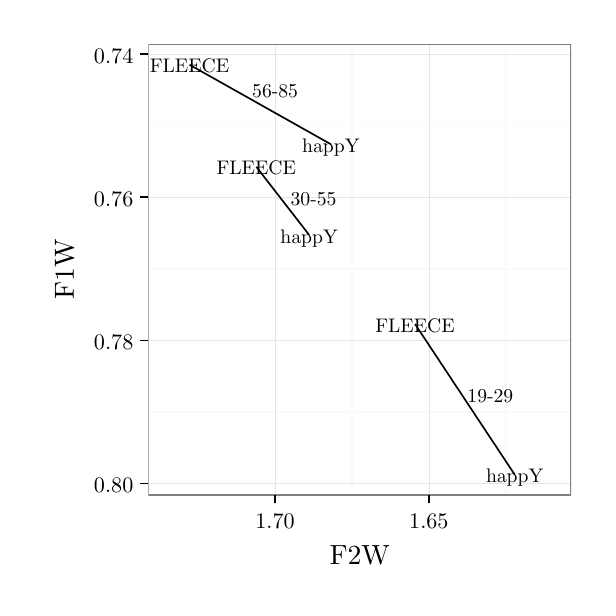
\begin{tikzpicture}[x=1pt,y=1pt]
\definecolor{fillColor}{RGB}{255,255,255}
\path[use as bounding box,fill=fillColor,fill opacity=0.00] (0,0) rectangle (202.36,202.36);
\begin{scope}
\path[clip] (  0.00,  0.00) rectangle (202.36,202.36);
\definecolor{drawColor}{RGB}{255,255,255}
\definecolor{fillColor}{RGB}{255,255,255}

\path[draw=drawColor,line width= 0.6pt,line join=round,line cap=round,fill=fillColor] (  0.00,  0.00) rectangle (202.36,202.36);
\end{scope}
\begin{scope}
\path[clip] ( 43.58, 33.48) rectangle (196.36,196.36);
\definecolor{fillColor}{RGB}{255,255,255}

\path[fill=fillColor] ( 43.58, 33.48) rectangle (196.36,196.36);
\definecolor{drawColor}{gray}{0.98}

\path[draw=drawColor,line width= 0.6pt,line join=round] ( 43.58,166.97) --
	(196.36,166.97);

\path[draw=drawColor,line width= 0.6pt,line join=round] ( 43.58,115.23) --
	(196.36,115.23);

\path[draw=drawColor,line width= 0.6pt,line join=round] ( 43.58, 63.50) --
	(196.36, 63.50);

\path[draw=drawColor,line width= 0.6pt,line join=round] (172.74, 33.48) --
	(172.74,196.36);

\path[draw=drawColor,line width= 0.6pt,line join=round] (117.19, 33.48) --
	(117.19,196.36);
\definecolor{drawColor}{gray}{0.90}

\path[draw=drawColor,line width= 0.2pt,line join=round] ( 43.58,192.83) --
	(196.36,192.83);

\path[draw=drawColor,line width= 0.2pt,line join=round] ( 43.58,141.10) --
	(196.36,141.10);

\path[draw=drawColor,line width= 0.2pt,line join=round] ( 43.58, 89.36) --
	(196.36, 89.36);

\path[draw=drawColor,line width= 0.2pt,line join=round] ( 43.58, 37.63) --
	(196.36, 37.63);

\path[draw=drawColor,line width= 0.2pt,line join=round] (144.97, 33.48) --
	(144.97,196.36);

\path[draw=drawColor,line width= 0.2pt,line join=round] ( 89.41, 33.48) --
	( 89.41,196.36);
\definecolor{drawColor}{RGB}{0,0,0}

\node[text=drawColor,anchor=base,inner sep=0pt, outer sep=0pt, scale=  0.71] at (109.55,157.29) {happY};

\node[text=drawColor,anchor=base,inner sep=0pt, outer sep=0pt, scale=  0.71] at ( 58.51,186.01) {FLEECE};

\node[text=drawColor,anchor=base,inner sep=0pt, outer sep=0pt, scale=  0.71] at (101.71,124.53) {happY};

\node[text=drawColor,anchor=base,inner sep=0pt, outer sep=0pt, scale=  0.71] at ( 82.62,149.14) {FLEECE};

\node[text=drawColor,anchor=base,inner sep=0pt, outer sep=0pt, scale=  0.71] at (175.97, 37.94) {happY};

\node[text=drawColor,anchor=base,inner sep=0pt, outer sep=0pt, scale=  0.71] at (139.97, 92.33) {FLEECE};

\path[draw=drawColor,line width= 0.6pt,line join=round] (109.55,160.23) --
	( 58.51,188.95);

\path[draw=drawColor,line width= 0.6pt,line join=round] (101.71,127.47) --
	( 82.62,152.08);

\path[draw=drawColor,line width= 0.6pt,line join=round] (175.97, 40.88) --
	(139.97, 95.27);

\node[text=drawColor,anchor=base,inner sep=0pt, outer sep=0pt, scale=  0.71] at ( 89.41,176.96) {56-85};

\node[text=drawColor,anchor=base,inner sep=0pt, outer sep=0pt, scale=  0.71] at (103.30,138.16) {30-55};

\node[text=drawColor,anchor=base,inner sep=0pt, outer sep=0pt, scale=  0.71] at (167.19, 67.02) {19-29};
\definecolor{drawColor}{gray}{0.50}

\path[draw=drawColor,line width= 0.6pt,line join=round,line cap=round] ( 43.58, 33.48) rectangle (196.36,196.36);
\end{scope}
\begin{scope}
\path[clip] (  0.00,  0.00) rectangle (202.36,202.36);
\definecolor{drawColor}{RGB}{0,0,0}

\node[text=drawColor,anchor=base east,inner sep=0pt, outer sep=0pt, scale=  0.80] at ( 38.18,189.53) {0.74};

\node[text=drawColor,anchor=base east,inner sep=0pt, outer sep=0pt, scale=  0.80] at ( 38.18,137.79) {0.76};

\node[text=drawColor,anchor=base east,inner sep=0pt, outer sep=0pt, scale=  0.80] at ( 38.18, 86.06) {0.78};

\node[text=drawColor,anchor=base east,inner sep=0pt, outer sep=0pt, scale=  0.80] at ( 38.18, 34.32) {0.80};
\end{scope}
\begin{scope}
\path[clip] (  0.00,  0.00) rectangle (202.36,202.36);
\definecolor{drawColor}{RGB}{0,0,0}

\path[draw=drawColor,line width= 0.6pt,line join=round] ( 40.58,192.83) --
	( 43.58,192.83);

\path[draw=drawColor,line width= 0.6pt,line join=round] ( 40.58,141.10) --
	( 43.58,141.10);

\path[draw=drawColor,line width= 0.6pt,line join=round] ( 40.58, 89.36) --
	( 43.58, 89.36);

\path[draw=drawColor,line width= 0.6pt,line join=round] ( 40.58, 37.63) --
	( 43.58, 37.63);
\end{scope}
\begin{scope}
\path[clip] (  0.00,  0.00) rectangle (202.36,202.36);
\definecolor{drawColor}{RGB}{0,0,0}

\path[draw=drawColor,line width= 0.6pt,line join=round] (144.97, 30.48) --
	(144.97, 33.48);

\path[draw=drawColor,line width= 0.6pt,line join=round] ( 89.41, 30.48) --
	( 89.41, 33.48);
\end{scope}
\begin{scope}
\path[clip] (  0.00,  0.00) rectangle (202.36,202.36);
\definecolor{drawColor}{RGB}{0,0,0}

\node[text=drawColor,anchor=base,inner sep=0pt, outer sep=0pt, scale=  0.80] at (144.97, 21.47) {1.65};

\node[text=drawColor,anchor=base,inner sep=0pt, outer sep=0pt, scale=  0.80] at ( 89.41, 21.47) {1.70};
\end{scope}
\begin{scope}
\path[clip] (  0.00,  0.00) rectangle (202.36,202.36);
\definecolor{drawColor}{RGB}{0,0,0}

\node[text=drawColor,anchor=base,inner sep=0pt, outer sep=0pt, scale=  1.00] at (119.97,  8.40) {F2W};
\end{scope}
\begin{scope}
\path[clip] (  0.00,  0.00) rectangle (202.36,202.36);
\definecolor{drawColor}{RGB}{0,0,0}

\node[text=drawColor,rotate= 90.00,anchor=base,inner sep=0pt, outer sep=0pt, scale=  1.00] at ( 16.67,114.92) {F1W};
\end{scope}
\end{tikzpicture}

	\caption{happ\textsc{y}-\textsc{fleece}: mean vowel position by age}
	\label{fig.happy.space.means}
\end{figure}

It \emph{does} look as if the majority of happ\textsc{y} realisations was marginally more retracted than most of the \textsc{fleece} variants in the young speakers, but since the centres of gravity of the vowel clouds are difficult to establish from Figure \ref{fig.happy.space}, it makes sense to consider a plot of the mean values (Figure \ref{fig.happy.space.means}).
This graph ignores the spread and overall distribution and only indicates where the means, i.e. the centres, of the \isi{exemplar} clouds are to be found.
Two pieces of information can be extracted from this figure.
Firstly, age groups cluster together: both mean \textsc{fleece} and happ\textsc{y} of the old speakers are higher than either vowel is on average in the middle-aged group.
The means for the latter group are, in turn, both more front and higher than either mean \textsc{fleece} or happ\textsc{y} of the youngest subjects in the sample.
The second point of interest in this graph is that the difference between the means of \textsc{fleece} and happ\textsc{y} is smallest for the middle-aged realisations, larger for the observations pertaining to the older subjects, and most pronounced in the sub-sample of Liverpudlians aged between 19 and 29.
This correlates with the fact that the p-value of the relevant \textsc{manova} was largest for the middle group, smaller for the old, and close to the 0.10 threshold for the youngest speakers, which indicates that mean realisations of happ\textsc{y} and \textsc{fleece} are indeed more robustly different among the old and the young speakers.

However, two caveats should be borne in mind:
\begin{inparaenum}[(1)]
	\item Figures \ref{fig.happy.space} and \ref{fig.happy.space.means} do not use the same scale --- the means of \textsc{fleece} and happ\textsc{y} are not identical, but the differences visible in Figure \ref{fig.happy.space.means} are actually very small.
	\item The previous point is corroborated by the \textsc{manova} results, which indicate almost perfect overlap between overall distributions (\isi{Pillai} scores near 0) and no significant difference between them (all p-values > 0.5).
\end{inparaenum}
The available statistical evidence thus clearly supports the claim that \textsc{fleece} and happ\textsc{y} are completely merged in all three age groups investigated.
Of course, this does not (directly) touch on the primary issue of \isi{change} in happ\textsc{y} across the three generations.
Figure \ref{fig.happy.space.means} corroborates the findings reported for F1 and F2 separately (and on the basis of mixed linear effects regressions): happ\textsc{y} becomes lower from the old to the middle-aged, and lower and \emph{more} central from the middle to the young speakers.

All of this only refers to rather formal realisations of these vowels, since the results in this section are exclusively based on the reading passage and the word list.
It remains to be seen whether the same conclusions would hold in spontaneous speech.

\section{\textsc{nurse}}
\label{sec.prod.res.vow.nurse}

\subsection{F1 (\textsc{nurse})}
\label{sec.prod.res.vow.nurse.f1}

\subsubsection{Overview}
\label{sec.prod.res.vow.nurse.f1.overview}

Just as with happ\textsc{y} results, the maximal model for \textsc{nurse} F1 measurements exhibited severe \isi{collinearity} (κ = 38.1).
Separate regression models showed that both place and manner of articulation of the following sound (κ = 34.25), and place of following consonant and \isi{frequency} of the carrier word (κ = 21.22) showed troubling or at least above average degrees of \isi{collinearity}.
Only one of these three, manner of articulation, was therefore retained.
In a second maximal model, which neither included place of articulation of preceding and following sound, nor \isi{frequency} of the keyword, \isi{collinearity} was acceptable (κ = 14.39).
The minimal adequate model (R\textsuperscript{2}-equivalent = 0.314) that was then derived is shown below (Table \ref{tab.regression.nurse.f1}).

{
	\footnotesize
	\begin{longtable}[c]{p{0.3\textwidth}rrrrrl}
		\caption{\textsc{nurse} (F1): mixed linear effects regression}\label{tab.regression.nurse.f1}\\
		
		\hline
		Fixed effects: & Estimate & Std. Error & df & t value & Pr($>$$|$t$|$) & \\ 
		\hline
		(Intercept) & 1.09 & 0.01 & 127.19 & 125.58 & < 0.001 & *** \\ 
		STYLElist & 0.03 & 0.01 & 1078.12 & 3.61 & < 0.001 & *** \\ 
		STYLEread & 0.00 & 0.01 & 1344.45 & 0.70 & 0.48 & \\ 
		STYLEfree & 0.00 & 0.01 & 362.94 & 0.48 & 0.63 & \\ 
		AGE56-85 & 0.02 & 0.01 & 1475.42 & 3.19 & < 0.01 & ** \\ 
		AGE30-55 & -0.01 & 0.01 & 1484.51 & -2.86 & < 0.01 & ** \\ 
		GENDERf & -0.03 & 0.00 & 1477.09 & -8.60 & < 0.001 & *** \\ 
		CLASSmc & 0.05 & 0.00 & 1479.04 & 12.16 & < 0.001 & *** \\ 
		PREMANNERaffr & -0.05 & 0.02 & 74.59 & -2.90 & < 0.01 & ** \\ 
		PREMANNERfric & -0.01 & 0.01 & 98.39 & -0.82 & 0.42 & \\ 
		PREMANNERgli & 0.01 & 0.01 & 65.20 & 0.54 & 0.59 & \\ 
		PREMANNERliq & 0.02 & 0.02 & 118.12 & 0.82 & 0.41 & \\ 
		PREMANNERnas & 0.02 & 0.02 & 377.34 & 0.95 & 0.34 & \\ 
		STYLElist:AGE56-85 & 0.02 & 0.01 & 1464.53 & 2.18 & 0.03 & * \\ 
		STYLEread:AGE56-85 & -0.01 & 0.01 & 1465.50 & -0.66 & 0.51 & \\ 
		STYLEfree:AGE56-85 & 0.01 & 0.01 & 1514.74 & 1.93 & 0.05 & .\\ 
		STYLElist:AGE30-55 & -0.01 & 0.01 & 1468.34 & -1.42 & 0.16 & \\ 
		STYLEread:AGE30-55 & 0.01 & 0.01 & 1470.78 & 0.80 & 0.42 & \\ 
		STYLEfree:AGE30-55 & -0.01 & 0.01 & 1513.20 & -0.89 & 0.37 & \\ 
		AGE56-85:GENDERf & -0.03 & 0.01 & 1475.15 & -5.98 & < 0.001 & *** \\ 
		AGE30-55:GENDERf & -0.01 & 0.01 & 1475.93 & -1.86 & 0.06 & .\\ 
		AGE56-85:CLASSmc & 0.02 & 0.01 & 1471.18 & 3.15 & < 0.01 & ** \\ 
		AGE30-55:CLASSmc & -0.01 & 0.01 & 1475.87 & -1.28 & 0.20 & \\ 
		GENDERf:CLASSmc & -0.01 & 0.00 & 1525.94 & -2.80 & 0.01 & **\\ 
		STYLElist:AGE56-85:GENDERf & 0.00 & 0.01 & 1464.29 & 0.25 & 0.80 & \\ 
		STYLEread:AGE56-85:GENDERf & 0.02 & 0.01 & 1464.64 & 1.26 & 0.21 & \\ 
		STYLEfree:AGE56-85:GENDERf & 0.02 & 0.01 & 1507.65 & 1.76 & 0.08 & .\\ 
		STYLElist:AGE30-55:GENDERf & 0.00 & 0.01 & 1466.69 & 0.40 & 0.69 & \\ 
		STYLEread:AGE30-55:GENDERf & -0.01 & 0.01 & 1473.07 & -1.07 & 0.28 & \\ 
		STYLEfree:AGE30-55:GENDERf & 0.01 & 0.01 & 1506.49 & 1.63 & 0.10 & \\ 
		STYLElist:AGE19-29:GENDERf & 0.01 & 0.01 & 1466.78 & 0.92 & 0.36 & \\ 
		STYLEread:AGE19-29:GENDERf & -0.00 & 0.01 & 1467.05 & -0.03 & 0.97 & \\ 
		STYLEfree:AGE19-29:GENDERf & -0.02 & 0.01 & 1519.51 & -2.30 & 0.02 & *\\ 
		STYLElist:AGE56-85:CLASSmc & 0.01 & 0.01 & 1463.33 & 0.52 & 0.60 & \\ 
		STYLEread:AGE56-85:CLASSmc & -0.02 & 0.01 & 1464.04 & -1.27 & 0.20 & \\ 
		STYLEfree:AGE56-85:CLASSmc & -0.02 & 0.01 & 1506.47 & -1.85 & 0.06 & .\\ 
		STYLElist:AGE30-55:CLASSmc & 0.02 & 0.01 & 1466.82 & 2.26 & 0.02 & * \\ 
		STYLEread:AGE30-55:CLASSmc & 0.01 & 0.01 & 1469.86 & 1.27 & 0.20 & \\ 
		STYLEfree:AGE30-55:CLASSmc & -0.02 & 0.01 & 1497.92 & -2.26 & 0.02 & * \\ 
		STYLElist:AGE19-29:CLASSmc & -0.00 & 0.01 & 1468.20 & -0.42 & 0.67 & \\ 
		STYLEread:AGE19-29:CLASSmc & 0.00 & 0.01 & 1468.92 & 0.19 & 0.85 & \\ 
		STYLEfree:AGE19-29:CLASSmc & 0.02 & 0.01 & 1516.74 & 2.46 & 0.01 & * \\ 
		\hline
		Random effects: & \multicolumn{6}{l}{(number of obs: 1568, groups: WORD, 137)} \\
		Groups &         Name & Variance &      Std.Dev. & & & \\
		WORD &  (Intercept) & 0.001 & 0.029 & & & \\
		Residual  &         & 0.011 & 0.103 & & & \\
		\hline
	\end{longtable}
}

It is immediately obvious that this model contains several additional significant predictors when compared to the corresponding model of happ\textsc{y}.
Style, age group, gender, and social class are again all significant main effects.
In addition, the model found significant interactions of style and age, age and class, age and gender, and gender and class.
Towards the bottom of the model we see that the interaction that is of greatest interest for this study, style X age, further entered into significant three-way interactions with both gender and social class.

Non-social factors, on the other hand, seem to be less important than for happ\textsc{y}, at least in relation to the social predictors: \isi{vowel duration}, manner of following consonant, and \isi{frequency} of the carrier word are all deleted as unsignificant during model reduction.
The only phonological predictor that is retained is manner of articulation of the preceding consonant\is{phonological context}, and even with this one there is only one level that is significantly different: \textsc{nurse} realisations are higher (i.e. more standard) when they are preceded by an affricate.
However, this only concerns a small minority of observations (97 out of 1770, or 5.48\%), which are relatively equally distributed across all styles, so this predictor will not be analysed any further here.

\subsubsection{Gender and class}
\label{sec.prod.res.vow.nurse.f1.genderclass}

Instead, we will move on to the interaction of gender and class.
Since the interaction is only one of degree (see below) the relevant graphs do not add much to the discussion and are therefore omitted.
In the group of middle-class speakers, men have a higher mean and median than women, which means that their \textsc{nurse} realisations are lower.
This difference is highly significant in the raw data (t(958.928) = -8.555, p < 0.001).
For working-class subjects, we have essentially the same situation: women have a lower average and median F1, indicating that they use more central variants of \textsc{nurse} (t(751.346) = -4.357, p < 0.001).
Technically speaking, the difference between women and men is somewhat less robust in the working class group (cf. the t-values of the two tests), but for all practical purposes the relationship is the same in both social classes as both t-tests yield p-values that are below 0.001.
The degree of the effect, however, is stronger in the middle class, meaning that there is a larger distance between the means of women and men in this class.

Conversely, the effect of social class is the same for both genders, although the difference between classes is smaller for women (t(813.931) = 7.824, p < 0.001), and more pronounced in the male group (t(941.869) = 13.469, p < 0.001).
Once again, however, this distinction is rather fine-grained as class differences are highly significant for both genders.
What is interesting, though, is that middle-class speakers actually use lower variants of \textsc{nurse} than their working-class counterparts.
This, in turn, holds for both genders, even though it is ever so slightly more pronounced in the male sub-sample.

\subsubsection{Gender and age}
\label{sec.prod.res.vow.nurse.f1.genderage}

\begin{figure}[h!]
	\centering
	\begin{subfigure}{.49\textwidth}
		\centering
			\definecolor{shadecolor}{rgb}{0.969, 0.969, 0.969}
			\resizebox{\linewidth}{!}{% Created by tikzDevice version 0.8.1 on 2016-02-09 02:14:27
% !TEX encoding = UTF-8 Unicode
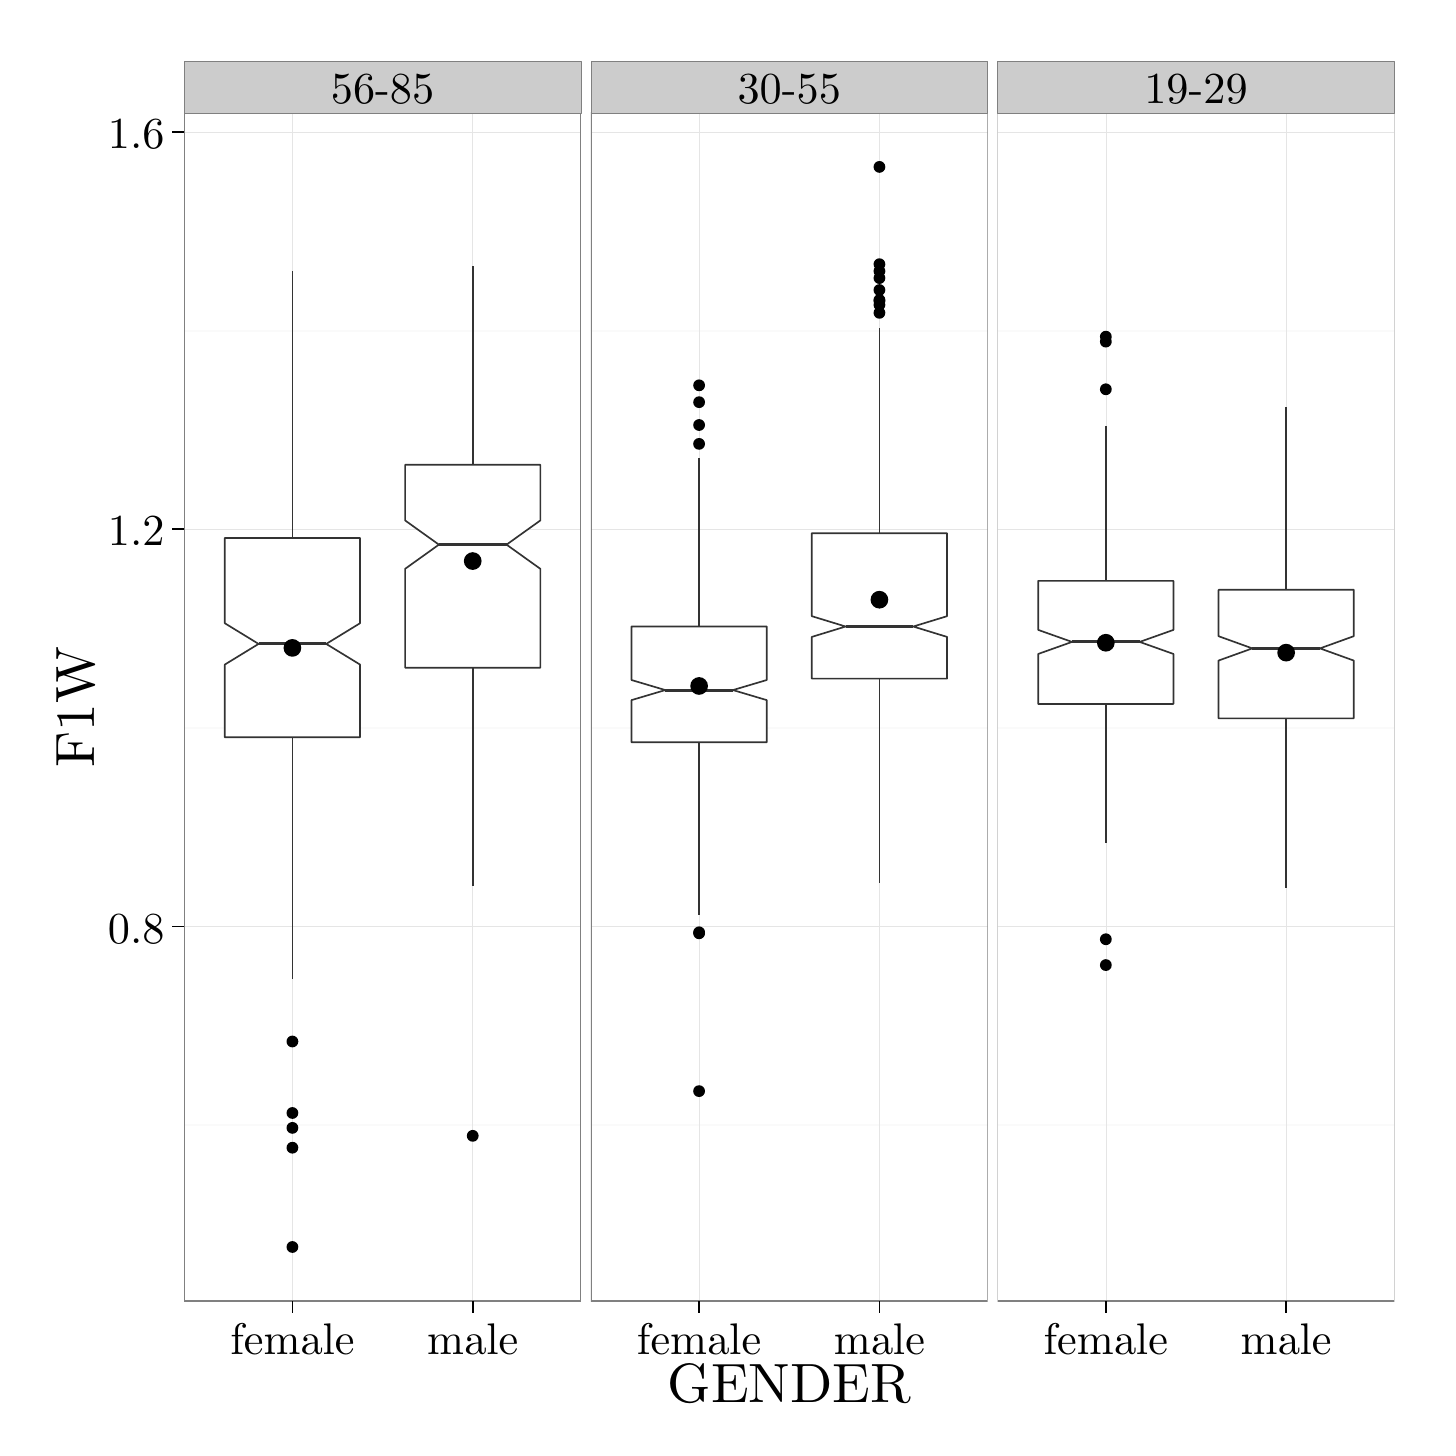
\begin{tikzpicture}[x=1pt,y=1pt]
\definecolor{fillColor}{RGB}{255,255,255}
\path[use as bounding box,fill=fillColor,fill opacity=0.00] (0,0) rectangle (505.89,505.89);
\begin{scope}
\path[clip] (  0.00,  0.00) rectangle (505.89,505.89);
\definecolor{drawColor}{RGB}{255,255,255}
\definecolor{fillColor}{RGB}{255,255,255}

\path[draw=drawColor,line width= 0.6pt,line join=round,line cap=round,fill=fillColor] (  0.00, -0.00) rectangle (505.89,505.89);
\end{scope}
\begin{scope}
\path[clip] ( 56.56, 45.77) rectangle (199.92,475.09);
\definecolor{fillColor}{RGB}{255,255,255}

\path[fill=fillColor] ( 56.56, 45.77) rectangle (199.92,475.09);
\definecolor{drawColor}{gray}{0.98}

\path[draw=drawColor,line width= 0.6pt,line join=round] ( 56.56,109.41) --
	(199.92,109.41);

\path[draw=drawColor,line width= 0.6pt,line join=round] ( 56.56,252.90) --
	(199.92,252.90);

\path[draw=drawColor,line width= 0.6pt,line join=round] ( 56.56,396.38) --
	(199.92,396.38);
\definecolor{drawColor}{gray}{0.90}

\path[draw=drawColor,line width= 0.2pt,line join=round] ( 56.56,181.15) --
	(199.92,181.15);

\path[draw=drawColor,line width= 0.2pt,line join=round] ( 56.56,324.64) --
	(199.92,324.64);

\path[draw=drawColor,line width= 0.2pt,line join=round] ( 56.56,468.13) --
	(199.92,468.13);

\path[draw=drawColor,line width= 0.2pt,line join=round] ( 95.66, 45.77) --
	( 95.66,475.09);

\path[draw=drawColor,line width= 0.2pt,line join=round] (160.82, 45.77) --
	(160.82,475.09);
\definecolor{fillColor}{RGB}{0,0,0}

\path[fill=fillColor] ( 95.66,139.54) circle (  2.13);

\path[fill=fillColor] ( 95.66,113.71) circle (  2.13);

\path[fill=fillColor] ( 95.66,108.33) circle (  2.13);

\path[fill=fillColor] ( 95.66, 65.29) circle (  2.13);

\path[fill=fillColor] ( 95.66,101.16) circle (  2.13);
\definecolor{drawColor}{gray}{0.20}

\path[draw=drawColor,line width= 0.6pt,line join=round] ( 95.66,321.50) -- ( 95.66,417.91);

\path[draw=drawColor,line width= 0.6pt,line join=round] ( 95.66,249.49) -- ( 95.66,162.14);
\definecolor{fillColor}{RGB}{255,255,255}

\path[draw=drawColor,line width= 0.6pt,line join=round,line cap=round,fill=fillColor] ( 71.23,321.50) --
	( 71.23,290.68) --
	( 83.44,283.21) --
	( 71.23,275.74) --
	( 71.23,249.49) --
	(120.10,249.49) --
	(120.10,275.74) --
	(107.88,283.21) --
	(120.10,290.68) --
	(120.10,321.50) --
	( 71.23,321.50) --
	cycle;

\path[draw=drawColor,line width= 1.1pt,line join=round] ( 83.44,283.21) -- (107.88,283.21);
\definecolor{fillColor}{RGB}{0,0,0}

\path[fill=fillColor] (160.82,105.46) circle (  2.13);

\path[draw=drawColor,line width= 0.6pt,line join=round] (160.82,347.96) -- (160.82,419.70);

\path[draw=drawColor,line width= 0.6pt,line join=round] (160.82,274.60) -- (160.82,195.86);
\definecolor{fillColor}{RGB}{255,255,255}

\path[draw=drawColor,line width= 0.6pt,line join=round,line cap=round,fill=fillColor] (136.39,347.96) --
	(136.39,327.82) --
	(148.60,319.08) --
	(136.39,310.34) --
	(136.39,274.60) --
	(185.25,274.60) --
	(185.25,310.34) --
	(173.04,319.08) --
	(185.25,327.82) --
	(185.25,347.96) --
	(136.39,347.96) --
	cycle;

\path[draw=drawColor,line width= 1.1pt,line join=round] (148.60,319.08) -- (173.04,319.08);
\definecolor{fillColor}{RGB}{0,0,0}

\path[fill=fillColor] ( 95.66,281.77) circle (  3.20);

\path[fill=fillColor] (160.82,313.15) circle (  3.20);
\definecolor{drawColor}{gray}{0.50}

\path[draw=drawColor,line width= 0.6pt,line join=round,line cap=round] ( 56.56, 45.77) rectangle (199.92,475.09);
\end{scope}
\begin{scope}
\path[clip] (203.53, 45.77) rectangle (346.88,475.09);
\definecolor{fillColor}{RGB}{255,255,255}

\path[fill=fillColor] (203.53, 45.77) rectangle (346.88,475.09);
\definecolor{drawColor}{gray}{0.98}

\path[draw=drawColor,line width= 0.6pt,line join=round] (203.53,109.41) --
	(346.88,109.41);

\path[draw=drawColor,line width= 0.6pt,line join=round] (203.53,252.90) --
	(346.88,252.90);

\path[draw=drawColor,line width= 0.6pt,line join=round] (203.53,396.38) --
	(346.88,396.38);
\definecolor{drawColor}{gray}{0.90}

\path[draw=drawColor,line width= 0.2pt,line join=round] (203.53,181.15) --
	(346.88,181.15);

\path[draw=drawColor,line width= 0.2pt,line join=round] (203.53,324.64) --
	(346.88,324.64);

\path[draw=drawColor,line width= 0.2pt,line join=round] (203.53,468.13) --
	(346.88,468.13);

\path[draw=drawColor,line width= 0.2pt,line join=round] (242.62, 45.77) --
	(242.62,475.09);

\path[draw=drawColor,line width= 0.2pt,line join=round] (307.78, 45.77) --
	(307.78,475.09);
\definecolor{fillColor}{RGB}{0,0,0}

\path[fill=fillColor] (242.62,179.00) circle (  2.13);

\path[fill=fillColor] (242.62,178.64) circle (  2.13);

\path[fill=fillColor] (242.62,121.61) circle (  2.13);

\path[fill=fillColor] (242.62,355.49) circle (  2.13);

\path[fill=fillColor] (242.62,362.31) circle (  2.13);

\path[fill=fillColor] (242.62,370.56) circle (  2.13);

\path[fill=fillColor] (242.62,376.65) circle (  2.13);
\definecolor{drawColor}{gray}{0.20}

\path[draw=drawColor,line width= 0.6pt,line join=round] (242.62,289.49) -- (242.62,350.47);

\path[draw=drawColor,line width= 0.6pt,line join=round] (242.62,247.70) -- (242.62,185.10);
\definecolor{fillColor}{RGB}{255,255,255}

\path[draw=drawColor,line width= 0.6pt,line join=round,line cap=round,fill=fillColor] (218.19,289.49) --
	(218.19,270.16) --
	(230.41,266.53) --
	(218.19,262.90) --
	(218.19,247.70) --
	(267.06,247.70) --
	(267.06,262.90) --
	(254.84,266.53) --
	(267.06,270.16) --
	(267.06,289.49) --
	(218.19,289.49) --
	cycle;

\path[draw=drawColor,line width= 1.1pt,line join=round] (230.41,266.53) -- (254.84,266.53);
\definecolor{fillColor}{RGB}{0,0,0}

\path[fill=fillColor] (307.78,415.40) circle (  2.13);

\path[fill=fillColor] (307.78,455.57) circle (  2.13);

\path[fill=fillColor] (307.78,420.42) circle (  2.13);

\path[fill=fillColor] (307.78,407.50) circle (  2.13);

\path[fill=fillColor] (307.78,417.91) circle (  2.13);

\path[fill=fillColor] (307.78,407.15) circle (  2.13);

\path[fill=fillColor] (307.78,402.84) circle (  2.13);

\path[fill=fillColor] (307.78,411.09) circle (  2.13);

\path[fill=fillColor] (307.78,405.71) circle (  2.13);

\path[draw=drawColor,line width= 0.6pt,line join=round] (307.78,323.21) -- (307.78,397.46);

\path[draw=drawColor,line width= 0.6pt,line join=round] (307.78,270.65) -- (307.78,196.94);
\definecolor{fillColor}{RGB}{255,255,255}

\path[draw=drawColor,line width= 0.6pt,line join=round,line cap=round,fill=fillColor] (283.35,323.21) --
	(283.35,293.23) --
	(295.57,289.49) --
	(283.35,285.74) --
	(283.35,270.65) --
	(332.22,270.65) --
	(332.22,285.74) --
	(320.00,289.49) --
	(332.22,293.23) --
	(332.22,323.21) --
	(283.35,323.21) --
	cycle;

\path[draw=drawColor,line width= 1.1pt,line join=round] (295.57,289.49) -- (320.00,289.49);
\definecolor{fillColor}{RGB}{0,0,0}

\path[fill=fillColor] (242.62,268.01) circle (  3.20);

\path[fill=fillColor] (307.78,299.18) circle (  3.20);
\definecolor{drawColor}{gray}{0.50}

\path[draw=drawColor,line width= 0.6pt,line join=round,line cap=round] (203.53, 45.77) rectangle (346.88,475.09);
\end{scope}
\begin{scope}
\path[clip] (350.49, 45.77) rectangle (493.85,475.09);
\definecolor{fillColor}{RGB}{255,255,255}

\path[fill=fillColor] (350.49, 45.77) rectangle (493.85,475.09);
\definecolor{drawColor}{gray}{0.98}

\path[draw=drawColor,line width= 0.6pt,line join=round] (350.49,109.41) --
	(493.85,109.41);

\path[draw=drawColor,line width= 0.6pt,line join=round] (350.49,252.90) --
	(493.85,252.90);

\path[draw=drawColor,line width= 0.6pt,line join=round] (350.49,396.38) --
	(493.85,396.38);
\definecolor{drawColor}{gray}{0.90}

\path[draw=drawColor,line width= 0.2pt,line join=round] (350.49,181.15) --
	(493.85,181.15);

\path[draw=drawColor,line width= 0.2pt,line join=round] (350.49,324.64) --
	(493.85,324.64);

\path[draw=drawColor,line width= 0.2pt,line join=round] (350.49,468.13) --
	(493.85,468.13);

\path[draw=drawColor,line width= 0.2pt,line join=round] (389.59, 45.77) --
	(389.59,475.09);

\path[draw=drawColor,line width= 0.2pt,line join=round] (454.75, 45.77) --
	(454.75,475.09);
\definecolor{fillColor}{RGB}{0,0,0}

\path[fill=fillColor] (389.59,375.22) circle (  2.13);

\path[fill=fillColor] (389.59,392.44) circle (  2.13);

\path[fill=fillColor] (389.59,394.23) circle (  2.13);

\path[fill=fillColor] (389.59,167.16) circle (  2.13);

\path[fill=fillColor] (389.59,176.49) circle (  2.13);
\definecolor{drawColor}{gray}{0.20}

\path[draw=drawColor,line width= 0.6pt,line join=round] (389.59,305.99) -- (389.59,361.95);

\path[draw=drawColor,line width= 0.6pt,line join=round] (389.59,261.51) -- (389.59,211.29);
\definecolor{fillColor}{RGB}{255,255,255}

\path[draw=drawColor,line width= 0.6pt,line join=round,line cap=round,fill=fillColor] (365.15,305.99) --
	(365.15,288.27) --
	(377.37,283.93) --
	(365.15,279.58) --
	(365.15,261.51) --
	(414.02,261.51) --
	(414.02,279.58) --
	(401.81,283.93) --
	(414.02,288.27) --
	(414.02,305.99) --
	(365.15,305.99) --
	cycle;

\path[draw=drawColor,line width= 1.1pt,line join=round] (377.37,283.93) -- (401.81,283.93);

\path[draw=drawColor,line width= 0.6pt,line join=round] (454.75,302.76) -- (454.75,368.76);

\path[draw=drawColor,line width= 0.6pt,line join=round] (454.75,256.30) -- (454.75,195.14);

\path[draw=drawColor,line width= 0.6pt,line join=round,line cap=round,fill=fillColor] (430.31,302.76) --
	(430.31,286.00) --
	(442.53,281.59) --
	(430.31,277.19) --
	(430.31,256.30) --
	(479.18,256.30) --
	(479.18,277.19) --
	(466.97,281.59) --
	(479.18,286.00) --
	(479.18,302.76) --
	(430.31,302.76) --
	cycle;

\path[draw=drawColor,line width= 1.1pt,line join=round] (442.53,281.59) -- (466.97,281.59);
\definecolor{fillColor}{RGB}{0,0,0}

\path[fill=fillColor] (389.59,283.63) circle (  3.20);

\path[fill=fillColor] (454.75,280.05) circle (  3.20);
\definecolor{drawColor}{gray}{0.50}

\path[draw=drawColor,line width= 0.6pt,line join=round,line cap=round] (350.49, 45.77) rectangle (493.85,475.09);
\end{scope}
\begin{scope}
\path[clip] (  0.00,  0.00) rectangle (505.89,505.89);
\definecolor{drawColor}{gray}{0.50}
\definecolor{fillColor}{gray}{0.80}

\path[draw=drawColor,line width= 0.2pt,line join=round,line cap=round,fill=fillColor] ( 56.56,475.09) rectangle (199.92,493.85);
\definecolor{drawColor}{RGB}{0,0,0}

\node[text=drawColor,anchor=base,inner sep=0pt, outer sep=0pt, scale=  1.60] at (128.24,478.43) {56-85};
\end{scope}
\begin{scope}
\path[clip] (  0.00,  0.00) rectangle (505.89,505.89);
\definecolor{drawColor}{gray}{0.50}
\definecolor{fillColor}{gray}{0.80}

\path[draw=drawColor,line width= 0.2pt,line join=round,line cap=round,fill=fillColor] (203.53,475.09) rectangle (346.88,493.85);
\definecolor{drawColor}{RGB}{0,0,0}

\node[text=drawColor,anchor=base,inner sep=0pt, outer sep=0pt, scale=  1.60] at (275.20,478.43) {30-55};
\end{scope}
\begin{scope}
\path[clip] (  0.00,  0.00) rectangle (505.89,505.89);
\definecolor{drawColor}{gray}{0.50}
\definecolor{fillColor}{gray}{0.80}

\path[draw=drawColor,line width= 0.2pt,line join=round,line cap=round,fill=fillColor] (350.49,475.09) rectangle (493.85,493.85);
\definecolor{drawColor}{RGB}{0,0,0}

\node[text=drawColor,anchor=base,inner sep=0pt, outer sep=0pt, scale=  1.60] at (422.17,478.43) {19-29};
\end{scope}
\begin{scope}
\path[clip] (  0.00,  0.00) rectangle (505.89,505.89);
\definecolor{drawColor}{RGB}{0,0,0}

\node[text=drawColor,anchor=base east,inner sep=0pt, outer sep=0pt, scale=  1.60] at ( 49.45,175.12) {0.8};

\node[text=drawColor,anchor=base east,inner sep=0pt, outer sep=0pt, scale=  1.60] at ( 49.45,318.61) {1.2};

\node[text=drawColor,anchor=base east,inner sep=0pt, outer sep=0pt, scale=  1.60] at ( 49.45,462.09) {1.6};
\end{scope}
\begin{scope}
\path[clip] (  0.00,  0.00) rectangle (505.89,505.89);
\definecolor{drawColor}{RGB}{0,0,0}

\path[draw=drawColor,line width= 0.6pt,line join=round] ( 52.30,181.15) --
	( 56.56,181.15);

\path[draw=drawColor,line width= 0.6pt,line join=round] ( 52.30,324.64) --
	( 56.56,324.64);

\path[draw=drawColor,line width= 0.6pt,line join=round] ( 52.30,468.13) --
	( 56.56,468.13);
\end{scope}
\begin{scope}
\path[clip] (  0.00,  0.00) rectangle (505.89,505.89);
\definecolor{drawColor}{RGB}{0,0,0}

\path[draw=drawColor,line width= 0.6pt,line join=round] ( 95.66, 41.50) --
	( 95.66, 45.77);

\path[draw=drawColor,line width= 0.6pt,line join=round] (160.82, 41.50) --
	(160.82, 45.77);
\end{scope}
\begin{scope}
\path[clip] (  0.00,  0.00) rectangle (505.89,505.89);
\definecolor{drawColor}{RGB}{0,0,0}

\node[text=drawColor,anchor=base,inner sep=0pt, outer sep=0pt, scale=  1.60] at ( 95.66, 26.59) {female};

\node[text=drawColor,anchor=base,inner sep=0pt, outer sep=0pt, scale=  1.60] at (160.82, 26.59) {male};
\end{scope}
\begin{scope}
\path[clip] (  0.00,  0.00) rectangle (505.89,505.89);
\definecolor{drawColor}{RGB}{0,0,0}

\path[draw=drawColor,line width= 0.6pt,line join=round] (242.62, 41.50) --
	(242.62, 45.77);

\path[draw=drawColor,line width= 0.6pt,line join=round] (307.78, 41.50) --
	(307.78, 45.77);
\end{scope}
\begin{scope}
\path[clip] (  0.00,  0.00) rectangle (505.89,505.89);
\definecolor{drawColor}{RGB}{0,0,0}

\node[text=drawColor,anchor=base,inner sep=0pt, outer sep=0pt, scale=  1.60] at (242.62, 26.59) {female};

\node[text=drawColor,anchor=base,inner sep=0pt, outer sep=0pt, scale=  1.60] at (307.78, 26.59) {male};
\end{scope}
\begin{scope}
\path[clip] (  0.00,  0.00) rectangle (505.89,505.89);
\definecolor{drawColor}{RGB}{0,0,0}

\path[draw=drawColor,line width= 0.6pt,line join=round] (389.59, 41.50) --
	(389.59, 45.77);

\path[draw=drawColor,line width= 0.6pt,line join=round] (454.75, 41.50) --
	(454.75, 45.77);
\end{scope}
\begin{scope}
\path[clip] (  0.00,  0.00) rectangle (505.89,505.89);
\definecolor{drawColor}{RGB}{0,0,0}

\node[text=drawColor,anchor=base,inner sep=0pt, outer sep=0pt, scale=  1.60] at (389.59, 26.59) {female};

\node[text=drawColor,anchor=base,inner sep=0pt, outer sep=0pt, scale=  1.60] at (454.75, 26.59) {male};
\end{scope}
\begin{scope}
\path[clip] (  0.00,  0.00) rectangle (505.89,505.89);
\definecolor{drawColor}{RGB}{0,0,0}

\node[text=drawColor,anchor=base,inner sep=0pt, outer sep=0pt, scale=  2.00] at (275.20,  9.03) {GENDER};
\end{scope}
\begin{scope}
\path[clip] (  0.00,  0.00) rectangle (505.89,505.89);
\definecolor{drawColor}{RGB}{0,0,0}

\node[text=drawColor,rotate= 90.00,anchor=base,inner sep=0pt, outer sep=0pt, scale=  2.00] at ( 24.12,260.43) {F1W};
\end{scope}
\end{tikzpicture}
} 
		\caption{box plot}
		\label{fig.box.f1w.nurse.genderage}
	\end{subfigure}
	\begin{subfigure}{.49\textwidth}
		\centering
			\definecolor{shadecolor}{rgb}{0.969, 0.969, 0.969}
			\resizebox{\linewidth}{!}{% Created by tikzDevice version 0.8.1 on 2016-02-09 02:14:30
% !TEX encoding = UTF-8 Unicode
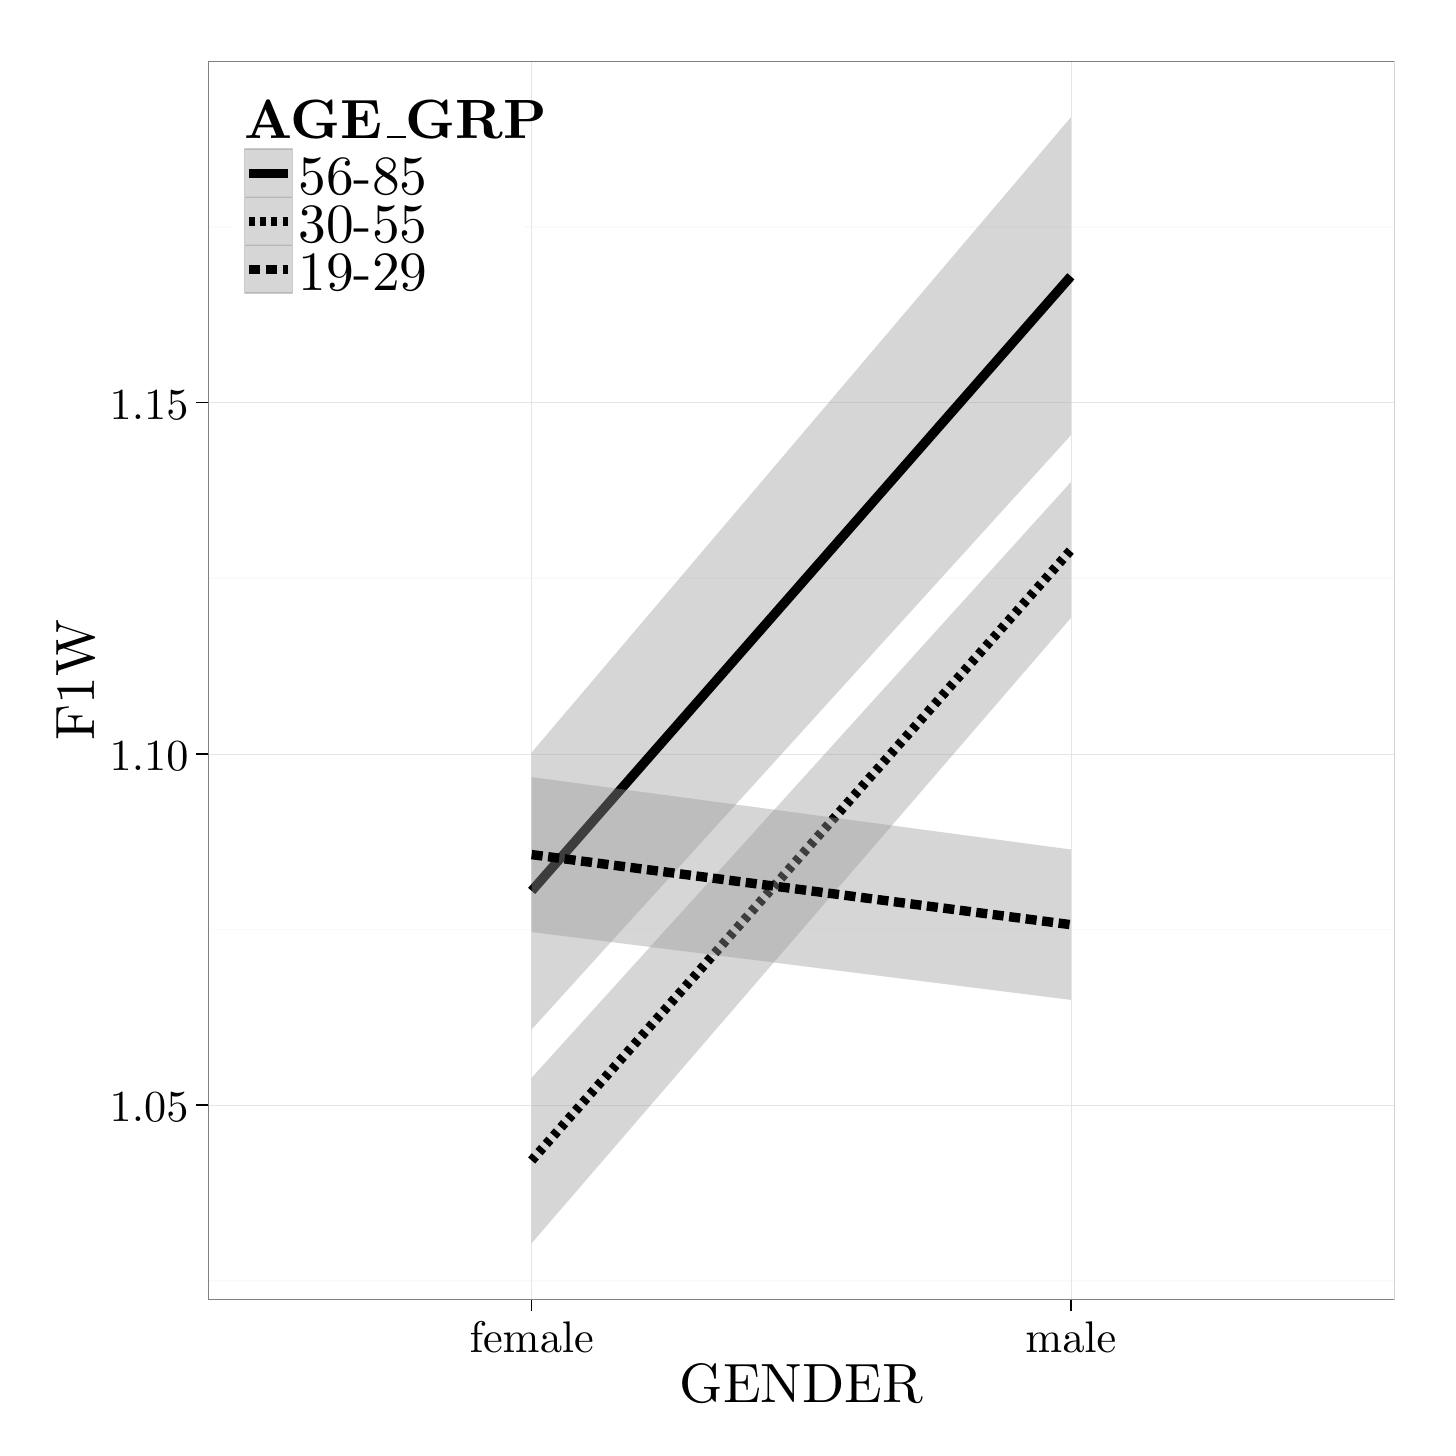
\begin{tikzpicture}[x=1pt,y=1pt]
\definecolor{fillColor}{RGB}{255,255,255}
\path[use as bounding box,fill=fillColor,fill opacity=0.00] (0,0) rectangle (505.89,505.89);
\begin{scope}
\path[clip] (  0.00,  0.00) rectangle (505.89,505.89);
\definecolor{drawColor}{RGB}{255,255,255}
\definecolor{fillColor}{RGB}{255,255,255}

\path[draw=drawColor,line width= 0.6pt,line join=round,line cap=round,fill=fillColor] (  0.00, -0.00) rectangle (505.89,505.89);
\end{scope}
\begin{scope}
\path[clip] ( 65.21, 46.31) rectangle (493.85,493.84);
\definecolor{fillColor}{RGB}{255,255,255}

\path[fill=fillColor] ( 65.21, 46.31) rectangle (493.85,493.84);
\definecolor{drawColor}{gray}{0.98}

\path[draw=drawColor,line width= 0.6pt,line join=round] ( 65.21, 53.01) --
	(493.85, 53.01);

\path[draw=drawColor,line width= 0.6pt,line join=round] ( 65.21,179.98) --
	(493.85,179.98);

\path[draw=drawColor,line width= 0.6pt,line join=round] ( 65.21,306.95) --
	(493.85,306.95);

\path[draw=drawColor,line width= 0.6pt,line join=round] ( 65.21,433.92) --
	(493.85,433.92);
\definecolor{drawColor}{gray}{0.90}

\path[draw=drawColor,line width= 0.2pt,line join=round] ( 65.21,116.50) --
	(493.85,116.50);

\path[draw=drawColor,line width= 0.2pt,line join=round] ( 65.21,243.46) --
	(493.85,243.46);

\path[draw=drawColor,line width= 0.2pt,line join=round] ( 65.21,370.43) --
	(493.85,370.43);

\path[draw=drawColor,line width= 0.2pt,line join=round] (182.11, 46.31) --
	(182.11,493.84);

\path[draw=drawColor,line width= 0.2pt,line join=round] (376.95, 46.31) --
	(376.95,493.84);
\definecolor{fillColor}{RGB}{153,153,153}

\path[fill=fillColor,fill opacity=0.40] (182.11,243.97) --
	(376.95,473.50) --
	(376.95,358.61) --
	(182.11,143.90) --
	cycle;
\definecolor{drawColor}{RGB}{0,0,0}

\path[draw=drawColor,line width= 3.4pt,line join=round] (182.11,193.94) --
	(376.95,416.05);

\path[fill=fillColor,fill opacity=0.40] (182.11,126.43) --
	(376.95,341.68) --
	(376.95,292.59) --
	(182.11, 66.65) --
	cycle;

\path[draw=drawColor,line width= 3.4pt,dash pattern=on 2pt off 2pt ,line join=round] (182.11, 96.54) --
	(376.95,317.14);

\path[fill=fillColor,fill opacity=0.40] (182.11,235.07) --
	(376.95,208.92) --
	(376.95,154.58) --
	(182.11,179.09) --
	cycle;

\path[draw=drawColor,line width= 3.4pt,dash pattern=on 4pt off 2pt ,line join=round] (182.11,207.08) --
	(376.95,181.75);
\definecolor{drawColor}{gray}{0.50}

\path[draw=drawColor,line width= 0.6pt,line join=round,line cap=round] ( 65.21, 46.31) rectangle (493.85,493.84);
\end{scope}
\begin{scope}
\path[clip] (  0.00,  0.00) rectangle (505.89,505.89);
\definecolor{drawColor}{RGB}{0,0,0}

\node[text=drawColor,anchor=base east,inner sep=0pt, outer sep=0pt, scale=  1.60] at ( 58.10,110.46) {1.05};

\node[text=drawColor,anchor=base east,inner sep=0pt, outer sep=0pt, scale=  1.60] at ( 58.10,237.43) {1.10};

\node[text=drawColor,anchor=base east,inner sep=0pt, outer sep=0pt, scale=  1.60] at ( 58.10,364.40) {1.15};
\end{scope}
\begin{scope}
\path[clip] (  0.00,  0.00) rectangle (505.89,505.89);
\definecolor{drawColor}{RGB}{0,0,0}

\path[draw=drawColor,line width= 0.6pt,line join=round] ( 60.95,116.50) --
	( 65.21,116.50);

\path[draw=drawColor,line width= 0.6pt,line join=round] ( 60.95,243.46) --
	( 65.21,243.46);

\path[draw=drawColor,line width= 0.6pt,line join=round] ( 60.95,370.43) --
	( 65.21,370.43);
\end{scope}
\begin{scope}
\path[clip] (  0.00,  0.00) rectangle (505.89,505.89);
\definecolor{drawColor}{RGB}{0,0,0}

\path[draw=drawColor,line width= 0.6pt,line join=round] (182.11, 42.04) --
	(182.11, 46.31);

\path[draw=drawColor,line width= 0.6pt,line join=round] (376.95, 42.04) --
	(376.95, 46.31);
\end{scope}
\begin{scope}
\path[clip] (  0.00,  0.00) rectangle (505.89,505.89);
\definecolor{drawColor}{RGB}{0,0,0}

\node[text=drawColor,anchor=base,inner sep=0pt, outer sep=0pt, scale=  1.60] at (182.11, 27.13) {female};

\node[text=drawColor,anchor=base,inner sep=0pt, outer sep=0pt, scale=  1.60] at (376.95, 27.13) {male};
\end{scope}
\begin{scope}
\path[clip] (  0.00,  0.00) rectangle (505.89,505.89);
\definecolor{drawColor}{RGB}{0,0,0}

\node[text=drawColor,anchor=base,inner sep=0pt, outer sep=0pt, scale=  2.00] at (279.53,  9.03) {GENDER};
\end{scope}
\begin{scope}
\path[clip] (  0.00,  0.00) rectangle (505.89,505.89);
\definecolor{drawColor}{RGB}{0,0,0}

\node[text=drawColor,rotate= 90.00,anchor=base,inner sep=0pt, outer sep=0pt, scale=  2.00] at ( 24.12,270.08) {F1W};
\end{scope}
\begin{scope}
\path[clip] (  0.00,  0.00) rectangle (505.89,505.89);
\definecolor{fillColor}{RGB}{255,255,255}

\path[fill=fillColor] ( 74.08,405.66) rectangle (179.78,484.98);
\end{scope}
\begin{scope}
\path[clip] (  0.00,  0.00) rectangle (505.89,505.89);
\definecolor{drawColor}{RGB}{0,0,0}

\node[text=drawColor,anchor=base west,inner sep=0pt, outer sep=0pt, scale=  2.00] at ( 78.35,465.96) {\bfseries AGE{\_{}}GRP};
\end{scope}
\begin{scope}
\path[clip] (  0.00,  0.00) rectangle (505.89,505.89);
\definecolor{drawColor}{gray}{0.80}
\definecolor{fillColor}{RGB}{255,255,255}

\path[draw=drawColor,line width= 0.6pt,line join=round,line cap=round,fill=fillColor] ( 78.35,444.61) rectangle ( 95.69,461.96);
\end{scope}
\begin{scope}
\path[clip] (  0.00,  0.00) rectangle (505.89,505.89);
\definecolor{fillColor}{RGB}{153,153,153}

\path[fill=fillColor,fill opacity=0.40] ( 78.35,444.61) rectangle ( 95.69,461.96);
\definecolor{drawColor}{RGB}{0,0,0}

\path[draw=drawColor,line width= 3.4pt,line join=round] ( 80.08,453.29) -- ( 93.96,453.29);
\end{scope}
\begin{scope}
\path[clip] (  0.00,  0.00) rectangle (505.89,505.89);
\definecolor{drawColor}{gray}{0.80}
\definecolor{fillColor}{RGB}{255,255,255}

\path[draw=drawColor,line width= 0.6pt,line join=round,line cap=round,fill=fillColor] ( 78.35,427.27) rectangle ( 95.69,444.61);
\end{scope}
\begin{scope}
\path[clip] (  0.00,  0.00) rectangle (505.89,505.89);
\definecolor{fillColor}{RGB}{153,153,153}

\path[fill=fillColor,fill opacity=0.40] ( 78.35,427.27) rectangle ( 95.69,444.61);
\definecolor{drawColor}{RGB}{0,0,0}

\path[draw=drawColor,line width= 3.4pt,dash pattern=on 2pt off 2pt ,line join=round] ( 80.08,435.94) -- ( 93.96,435.94);
\end{scope}
\begin{scope}
\path[clip] (  0.00,  0.00) rectangle (505.89,505.89);
\definecolor{drawColor}{gray}{0.80}
\definecolor{fillColor}{RGB}{255,255,255}

\path[draw=drawColor,line width= 0.6pt,line join=round,line cap=round,fill=fillColor] ( 78.35,409.92) rectangle ( 95.69,427.27);
\end{scope}
\begin{scope}
\path[clip] (  0.00,  0.00) rectangle (505.89,505.89);
\definecolor{fillColor}{RGB}{153,153,153}

\path[fill=fillColor,fill opacity=0.40] ( 78.35,409.92) rectangle ( 95.69,427.27);
\definecolor{drawColor}{RGB}{0,0,0}

\path[draw=drawColor,line width= 3.4pt,dash pattern=on 4pt off 2pt ,line join=round] ( 80.08,418.60) -- ( 93.96,418.60);
\end{scope}
\begin{scope}
\path[clip] (  0.00,  0.00) rectangle (505.89,505.89);
\definecolor{drawColor}{RGB}{0,0,0}

\node[text=drawColor,anchor=base west,inner sep=0pt, outer sep=0pt, scale=  2.00] at ( 97.86,445.75) {56-85};
\end{scope}
\begin{scope}
\path[clip] (  0.00,  0.00) rectangle (505.89,505.89);
\definecolor{drawColor}{RGB}{0,0,0}

\node[text=drawColor,anchor=base west,inner sep=0pt, outer sep=0pt, scale=  2.00] at ( 97.86,428.40) {30-55};
\end{scope}
\begin{scope}
\path[clip] (  0.00,  0.00) rectangle (505.89,505.89);
\definecolor{drawColor}{RGB}{0,0,0}

\node[text=drawColor,anchor=base west,inner sep=0pt, outer sep=0pt, scale=  2.00] at ( 97.86,411.06) {19-29};
\end{scope}
\end{tikzpicture}
} 
		\caption{regression plot}
		\label{fig.scatter.f1w.nurse.genderage}
	\end{subfigure}
	\caption{\textsc{nurse} (F1) by gender and age}
\end{figure}

The interaction of gender and age is somewhat more interesting in this respect.
Looking at gender differences in the oldest speakers (left panel of Figure \ref{fig.box.f1w.nurse.genderage}) we find that women have considerably lower F1 values than men.
The \isi{gender effect} is highly significant (t(395.594) = -5.823, p < 0.001): men realise \textsc{nurse} as a lower vowel than women.
The same relation holds in the middle age group.
Men again have higher F1 values on average than women.
Judging from the box plot, which suggests less variation (smaller boxes) and smaller median confidence intervals (width of the notches), this difference is even more significant than for the oldest speakers.
A t-test supports this impression (t(805.568) = -11.767, p < 0.001), although it has to be said that
\begin{inparaenum}[(a)]
	\item this could simply be due to the fact that there are less data for the oldest speakers, and
	\item the difference is already highly significant in the old group.
\end{inparaenum}
The youngest subjects in the sample differ markedly from speakers of their parents' or grandparents' generation, because in this group there is no significant difference between male and female \textsc{nurse} realisations (t(537.587) = 1.277, p = 0.202).
Both means (and medians) are on a level which is almost perfectly intermediate between the means of middle-aged female and male speakers.

This non-significant difference between genders is also visible in Figure \ref{fig.scatter.f1w.nurse.genderage}, which has a (dashed) regression line for the youngest interviewees which is almost parallel to the x-axis of the plot.
The comparatively steep positive slopes of the other two lines that stand for the old (solid) and middle-aged subjects (dotted), in turn visualise the gender difference that is already evident in Figure \ref{fig.box.f1w.nurse.genderage}.
The regression plot also shows that all age groups seem to be significantly different from one another as far as the male speakers are concerned: the lines are clearly distinct and standard deviations (grey areas) do not overlap.
One can reach the same conclusion based on the t-tests summarised in Table \ref{tab.nurse.genderage.pvalues}, which confirm that all three age groups are (highly) significant when the analysis is restricted to male subjects.
In the female sub-sample, on the other hand, the middle age group is different from the other two, but the oldest and the youngest speakers do not differ with respect to the height of \textsc{nurse} (cf. the t-tests in Table \ref{tab.nurse.genderage.pvalues} and the standard error margins in Figure \ref{fig.scatter.f1w.nurse.genderage}).
It looks thus as if male Scousers have constantly raised \textsc{nurse} over the time period investigated here (if only to a very small extent in absolute terms), while female speakers first slightly raised \textsc{nurse} from the oldest to the middle-aged speakers, only to return to the starting point again in the youngest group.
Since this starting point is statistically identical to the one the youngest male speakers have arrived at, the gender difference is therefore gone in this age group.

\begin{table}[h!]
	\centering
	\caption{\textsc{nurse} (F1): t-tests of age by gender}
	\label{tab.nurse.genderage.pvalues}
	\begin{tabular}{lrrrrrr}
		\hline
		test & \multicolumn{3}{c}{women} & \multicolumn{3}{c}{men}\\
		& t & df & p & t & df & p\\
		\hline
		old-middle & \ensuremath{-3.292} & 337.596 & 0.001 & \ensuremath{-3.242} & 267.935 & 0.001\\
		middle-young & 5.819 & 566.832 & < 0.001 & \ensuremath{-6.908} & 697.042 & < 0.001\\
		young-old & 0.436 & 352.420 & 0.663 & \ensuremath{-7.637} & 268.135 & < 0.001\\			 
		\hline			
	\end{tabular}
\end{table}

\subsubsection{Age and class}
\label{sec.prod.res.vow.nurse.f1.ageclass}

When it comes to the interplay of age and social class we have again a case where one might wonder why this interaction was found to be significant in the mixed linear effects regression.
There are, once more, only differences in degree so the box and regression plots are not printed here (cf. \ref{sec.prod.res.vow.nurse.f1.genderclass}).
As reported above, middle-class speakers have higher F1 values (which translate to more open, i.e. more Scouse \textsc{nurse} variants) than working-class Liverpudlians.
This holds across all age groups and the difference is highly significant in the old (t(403.191) = 5.927, p < 0.001), the middle (t(798.733) = 10.566, p < 0.001), \emph{and} the young group (t(534.588) = 11.88, p < 0.001), so an interaction does not seem `necessary'.\footnote{A box plot based on the values predicted by the regression model (instead of the actually observed ones) was also generated to visualise the interaction once the random effects have been accounted for. This graph, however, did not look markedly different and is therefore not reprinted here either.}

Closer inspection of the figures nevertheless reveals tiny differences.
The t-tests reported in Table \ref{tab.nurse.classage.pvalues} provide evidence that the middle-aged and the young group are not significantly different, neither in the working, nor the middle-class sub-sample.
\textsc{nurse} productions of the oldest speakers, on the other hand, seem to be distinct from the other two groups, both in the middle and the working-class sub-sample.
In the raw data, p-values are only a bit higher for the working-class observations (but still below the 5\% threshold, so \textsc{nurse} variants in the oldest group \emph{are} significantly different from the rest), but this slight deviation seems to be enough for the interaction to surface as significant in the mixed-effects model.

\begin{table}[h!]
	\centering
	\caption{\textsc{nurse} (F1): t-tests of age by social class}
	\label{tab.nurse.classage.pvalues}
	\begin{tabular}{lrrrrrr}
		\hline
		test & \multicolumn{3}{c}{middle class} & \multicolumn{3}{c}{working class}\\
		& t & df & p & t & df & p\\
		\hline
		old-middle & \ensuremath{-2.950} & 342.020 & 0.003 & \ensuremath{-2.064} & 266.401 & 0.040\\
		middle-young & 0.479 & 700.025 & 0.632 & \ensuremath{-0.119} & 610.856 & 0.905\\
		young-old & \ensuremath{-2.727} & 307.814 & 0.007 & \ensuremath{-2.133} & 267.448 & 0.034\\			 
		\hline			
	\end{tabular}
\end{table}

Let us take a step back and briefly consider age of participant as a main effect before we investigate the interaction with speaking style.
A box plot (Figure \ref{fig.box.f1.nurse.tot}) clearly shows that the oldest subjects have a higher F1 for \textsc{nurse} than both the middle and the young group.
The difference between the old and the middle-aged group looks significant, and is indeed found to be so by a t-test on the raw data (t(634.126) = -2.735, p = 0.006).
Equally significant (t(1322.803) = -2.387, p = 0.017) is the drop from the middle to the young group, even though the virtually identical medians and the notches of the boxes might suggest otherwise.
Young speakers in my sample thus have a significantly more close \textsc{nurse} realisation than speakers of the other age ranges.

\begin{figure}[h!]
	\centering
		\definecolor{shadecolor}{rgb}{0.969, 0.969, 0.969}
		\resizebox{0.5\linewidth}{!}{% Created by tikzDevice version 0.8.1 on 2016-02-09 02:14:37
% !TEX encoding = UTF-8 Unicode
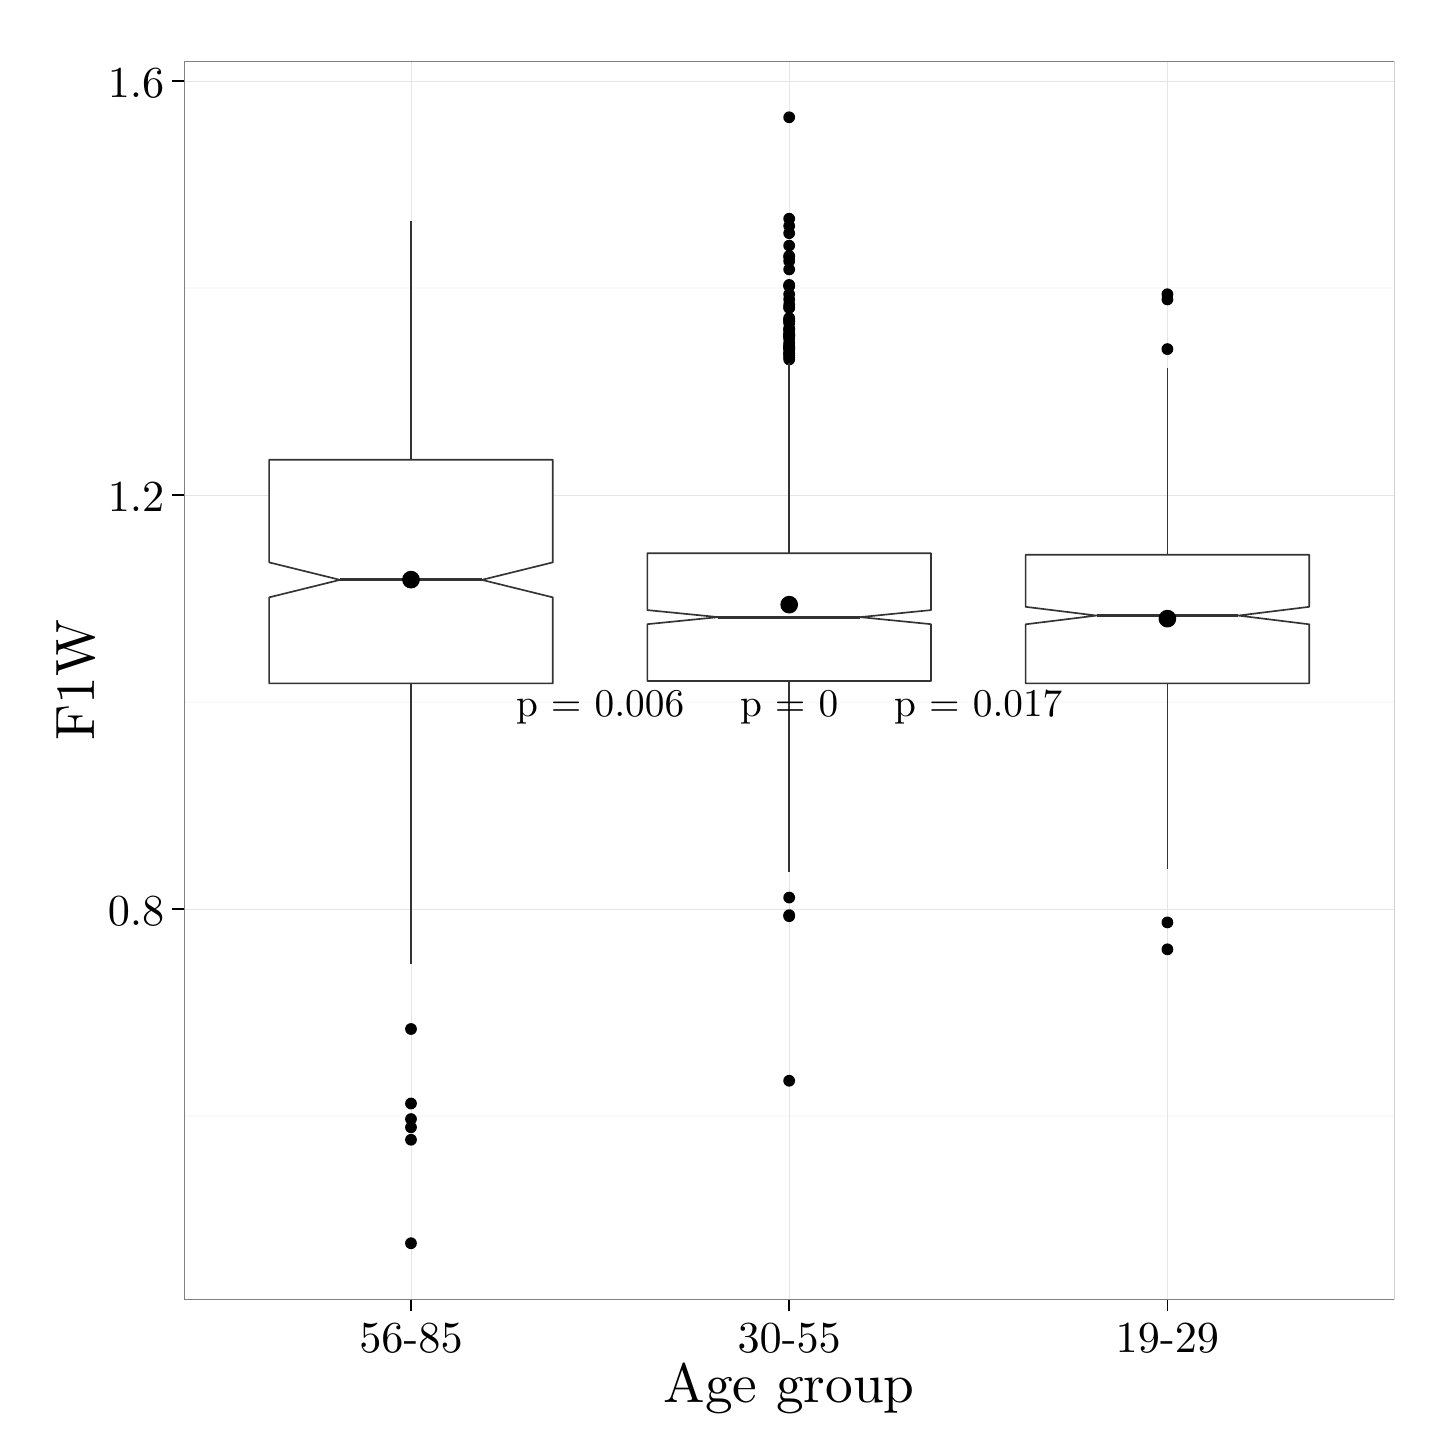
\begin{tikzpicture}[x=1pt,y=1pt]
\definecolor{fillColor}{RGB}{255,255,255}
\path[use as bounding box,fill=fillColor,fill opacity=0.00] (0,0) rectangle (505.89,505.89);
\begin{scope}
\path[clip] (  0.00,  0.00) rectangle (505.89,505.89);
\definecolor{drawColor}{RGB}{255,255,255}
\definecolor{fillColor}{RGB}{255,255,255}

\path[draw=drawColor,line width= 0.6pt,line join=round,line cap=round,fill=fillColor] (  0.00, -0.00) rectangle (505.89,505.89);
\end{scope}
\begin{scope}
\path[clip] ( 56.50, 46.31) rectangle (493.85,493.84);
\definecolor{fillColor}{RGB}{255,255,255}

\path[fill=fillColor] ( 56.50, 46.31) rectangle (493.85,493.84);
\definecolor{drawColor}{gray}{0.98}

\path[draw=drawColor,line width= 0.6pt,line join=round] ( 56.50,112.65) --
	(493.85,112.65);

\path[draw=drawColor,line width= 0.6pt,line join=round] ( 56.50,262.22) --
	(493.85,262.22);

\path[draw=drawColor,line width= 0.6pt,line join=round] ( 56.50,411.80) --
	(493.85,411.80);
\definecolor{drawColor}{gray}{0.90}

\path[draw=drawColor,line width= 0.2pt,line join=round] ( 56.50,187.43) --
	(493.85,187.43);

\path[draw=drawColor,line width= 0.2pt,line join=round] ( 56.50,337.01) --
	(493.85,337.01);

\path[draw=drawColor,line width= 0.2pt,line join=round] ( 56.50,486.59) --
	(493.85,486.59);

\path[draw=drawColor,line width= 0.2pt,line join=round] (138.51, 46.31) --
	(138.51,493.84);

\path[draw=drawColor,line width= 0.2pt,line join=round] (275.17, 46.31) --
	(275.17,493.84);

\path[draw=drawColor,line width= 0.2pt,line join=round] (411.84, 46.31) --
	(411.84,493.84);
\definecolor{fillColor}{RGB}{0,0,0}

\path[fill=fillColor] (138.51,108.53) circle (  2.13);

\path[fill=fillColor] (138.51,144.06) circle (  2.13);

\path[fill=fillColor] (138.51,117.13) circle (  2.13);

\path[fill=fillColor] (138.51,111.52) circle (  2.13);

\path[fill=fillColor] (138.51, 66.65) circle (  2.13);

\path[fill=fillColor] (138.51,104.04) circle (  2.13);
\definecolor{drawColor}{gray}{0.20}

\path[draw=drawColor,line width= 0.6pt,line join=round] (138.51,349.73) -- (138.51,436.11);

\path[draw=drawColor,line width= 0.6pt,line join=round] (138.51,268.95) -- (138.51,167.62);
\definecolor{fillColor}{RGB}{255,255,255}

\path[draw=drawColor,line width= 0.6pt,line join=round,line cap=round,fill=fillColor] ( 87.25,349.73) --
	( 87.25,312.67) --
	(112.88,306.35) --
	( 87.25,300.03) --
	( 87.25,268.95) --
	(189.76,268.95) --
	(189.76,300.03) --
	(164.13,306.35) --
	(189.76,312.67) --
	(189.76,349.73) --
	( 87.25,349.73) --
	cycle;

\path[draw=drawColor,line width= 1.1pt,line join=round] (112.88,306.35) -- (164.13,306.35);
\definecolor{fillColor}{RGB}{0,0,0}

\path[fill=fillColor] (275.17,396.84) circle (  2.13);

\path[fill=fillColor] (275.17,431.62) circle (  2.13);

\path[fill=fillColor] (275.17,399.84) circle (  2.13);

\path[fill=fillColor] (275.17,473.50) circle (  2.13);

\path[fill=fillColor] (275.17,436.86) circle (  2.13);

\path[fill=fillColor] (275.17,423.39) circle (  2.13);

\path[fill=fillColor] (275.17,394.60) circle (  2.13);

\path[fill=fillColor] (275.17,390.49) circle (  2.13);

\path[fill=fillColor] (275.17,390.49) circle (  2.13);

\path[fill=fillColor] (275.17,409.56) circle (  2.13);

\path[fill=fillColor] (275.17,412.92) circle (  2.13);

\path[fill=fillColor] (275.17,405.82) circle (  2.13);

\path[fill=fillColor] (275.17,396.47) circle (  2.13);

\path[fill=fillColor] (275.17,389.74) circle (  2.13);

\path[fill=fillColor] (275.17,434.24) circle (  2.13);

\path[fill=fillColor] (275.17,389.74) circle (  2.13);

\path[fill=fillColor] (275.17,400.58) circle (  2.13);

\path[fill=fillColor] (275.17,399.84) circle (  2.13);

\path[fill=fillColor] (275.17,400.96) circle (  2.13);

\path[fill=fillColor] (275.17,423.02) circle (  2.13);

\path[fill=fillColor] (275.17,388.24) circle (  2.13);

\path[fill=fillColor] (275.17,394.60) circle (  2.13);

\path[fill=fillColor] (275.17,391.98) circle (  2.13);

\path[fill=fillColor] (275.17,386.00) circle (  2.13);

\path[fill=fillColor] (275.17,404.70) circle (  2.13);

\path[fill=fillColor] (275.17,412.55) circle (  2.13);

\path[fill=fillColor] (275.17,412.55) circle (  2.13);

\path[fill=fillColor] (275.17,395.35) circle (  2.13);

\path[fill=fillColor] (275.17,394.97) circle (  2.13);

\path[fill=fillColor] (275.17,418.53) circle (  2.13);

\path[fill=fillColor] (275.17,407.69) circle (  2.13);

\path[fill=fillColor] (275.17,387.50) circle (  2.13);

\path[fill=fillColor] (275.17,388.24) circle (  2.13);

\path[fill=fillColor] (275.17,399.09) circle (  2.13);

\path[fill=fillColor] (275.17,390.49) circle (  2.13);

\path[fill=fillColor] (275.17,427.13) circle (  2.13);

\path[fill=fillColor] (275.17,386.75) circle (  2.13);

\path[fill=fillColor] (275.17,404.70) circle (  2.13);

\path[fill=fillColor] (275.17,421.52) circle (  2.13);

\path[fill=fillColor] (275.17,393.48) circle (  2.13);

\path[fill=fillColor] (275.17,394.23) circle (  2.13);

\path[fill=fillColor] (275.17,397.22) circle (  2.13);

\path[fill=fillColor] (275.17,185.19) circle (  2.13);

\path[fill=fillColor] (275.17,184.82) circle (  2.13);

\path[fill=fillColor] (275.17,125.36) circle (  2.13);

\path[fill=fillColor] (275.17,191.55) circle (  2.13);

\path[fill=fillColor] (275.17,391.23) circle (  2.13);

\path[draw=drawColor,line width= 0.6pt,line join=round] (275.17,315.98) -- (275.17,384.88);

\path[draw=drawColor,line width= 0.6pt,line join=round] (275.17,269.80) -- (275.17,200.90);
\definecolor{fillColor}{RGB}{255,255,255}

\path[draw=drawColor,line width= 0.6pt,line join=round,line cap=round,fill=fillColor] (223.92,315.98) --
	(223.92,295.43) --
	(249.55,292.89) --
	(223.92,290.34) --
	(223.92,269.80) --
	(326.43,269.80) --
	(326.43,290.34) --
	(300.80,292.89) --
	(326.43,295.43) --
	(326.43,315.98) --
	(223.92,315.98) --
	cycle;

\path[draw=drawColor,line width= 1.1pt,line join=round] (249.55,292.89) -- (300.80,292.89);
\definecolor{fillColor}{RGB}{0,0,0}

\path[fill=fillColor] (411.84,389.74) circle (  2.13);

\path[fill=fillColor] (411.84,407.69) circle (  2.13);

\path[fill=fillColor] (411.84,409.56) circle (  2.13);

\path[fill=fillColor] (411.84,172.85) circle (  2.13);

\path[fill=fillColor] (411.84,182.57) circle (  2.13);

\path[draw=drawColor,line width= 0.6pt,line join=round] (411.84,315.42) -- (411.84,383.01);

\path[draw=drawColor,line width= 0.6pt,line join=round] (411.84,268.95) -- (411.84,202.02);
\definecolor{fillColor}{RGB}{255,255,255}

\path[draw=drawColor,line width= 0.6pt,line join=round,line cap=round,fill=fillColor] (360.59,315.42) --
	(360.59,296.61) --
	(386.22,293.45) --
	(360.59,290.29) --
	(360.59,268.95) --
	(463.09,268.95) --
	(463.09,290.29) --
	(437.47,293.45) --
	(463.09,296.61) --
	(463.09,315.42) --
	(360.59,315.42) --
	cycle;

\path[draw=drawColor,line width= 1.1pt,line join=round] (386.22,293.45) -- (437.47,293.45);
\definecolor{fillColor}{RGB}{0,0,0}

\path[fill=fillColor] (138.51,306.43) circle (  3.20);

\path[fill=fillColor] (275.17,297.39) circle (  3.20);

\path[fill=fillColor] (411.84,292.34) circle (  3.20);
\definecolor{drawColor}{RGB}{0,0,0}

\node[text=drawColor,anchor=base,inner sep=0pt, outer sep=0pt, scale=  1.42] at (206.84,256.88) {p = 0.006};

\node[text=drawColor,anchor=base,inner sep=0pt, outer sep=0pt, scale=  1.42] at (343.51,256.88) {p = 0.017};

\node[text=drawColor,anchor=base,inner sep=0pt, outer sep=0pt, scale=  1.42] at (275.17,256.88) {p = 0};
\definecolor{drawColor}{gray}{0.50}

\path[draw=drawColor,line width= 0.6pt,line join=round,line cap=round] ( 56.50, 46.31) rectangle (493.85,493.84);
\end{scope}
\begin{scope}
\path[clip] (  0.00,  0.00) rectangle (505.89,505.89);
\definecolor{drawColor}{RGB}{0,0,0}

\node[text=drawColor,anchor=base east,inner sep=0pt, outer sep=0pt, scale=  1.60] at ( 49.39,181.40) {0.8};

\node[text=drawColor,anchor=base east,inner sep=0pt, outer sep=0pt, scale=  1.60] at ( 49.39,330.98) {1.2};

\node[text=drawColor,anchor=base east,inner sep=0pt, outer sep=0pt, scale=  1.60] at ( 49.39,480.56) {1.6};
\end{scope}
\begin{scope}
\path[clip] (  0.00,  0.00) rectangle (505.89,505.89);
\definecolor{drawColor}{RGB}{0,0,0}

\path[draw=drawColor,line width= 0.6pt,line join=round] ( 52.24,187.43) --
	( 56.50,187.43);

\path[draw=drawColor,line width= 0.6pt,line join=round] ( 52.24,337.01) --
	( 56.50,337.01);

\path[draw=drawColor,line width= 0.6pt,line join=round] ( 52.24,486.59) --
	( 56.50,486.59);
\end{scope}
\begin{scope}
\path[clip] (  0.00,  0.00) rectangle (505.89,505.89);
\definecolor{drawColor}{RGB}{0,0,0}

\path[draw=drawColor,line width= 0.6pt,line join=round] (138.51, 42.04) --
	(138.51, 46.31);

\path[draw=drawColor,line width= 0.6pt,line join=round] (275.17, 42.04) --
	(275.17, 46.31);

\path[draw=drawColor,line width= 0.6pt,line join=round] (411.84, 42.04) --
	(411.84, 46.31);
\end{scope}
\begin{scope}
\path[clip] (  0.00,  0.00) rectangle (505.89,505.89);
\definecolor{drawColor}{RGB}{0,0,0}

\node[text=drawColor,anchor=base,inner sep=0pt, outer sep=0pt, scale=  1.60] at (138.51, 27.13) {56-85};

\node[text=drawColor,anchor=base,inner sep=0pt, outer sep=0pt, scale=  1.60] at (275.17, 27.13) {30-55};

\node[text=drawColor,anchor=base,inner sep=0pt, outer sep=0pt, scale=  1.60] at (411.84, 27.13) {19-29};
\end{scope}
\begin{scope}
\path[clip] (  0.00,  0.00) rectangle (505.89,505.89);
\definecolor{drawColor}{RGB}{0,0,0}

\node[text=drawColor,anchor=base,inner sep=0pt, outer sep=0pt, scale=  2.00] at (275.17,  9.03) {Age group};
\end{scope}
\begin{scope}
\path[clip] (  0.00,  0.00) rectangle (505.89,505.89);
\definecolor{drawColor}{RGB}{0,0,0}

\node[text=drawColor,rotate= 90.00,anchor=base,inner sep=0pt, outer sep=0pt, scale=  2.00] at ( 24.12,270.08) {F1W};
\end{scope}
\end{tikzpicture}
} 
	\caption{\textsc{nurse} (F1) by age}
	\label{fig.box.f1.nurse.tot}
\end{figure}

\subsubsection{Style shifting}
\label{sec.prod.res.vow.nurse.f1.shifting}

The interaction of style and age (along with the two three-way interactions of style, age, and gender and class, respectively) are visualised by a number of line plots which are all structured similarly and were already used in Sections \ref{sec.prod.res.vow.happy.f1} and \ref{sec.prod.res.vow.happy.f2}: style is marked on the x-axis, F1 on the y-axis, and age group of participant is coded by line type.

\begin{figure}[h!]
	\centering
		\definecolor{shadecolor}{rgb}{0.969, 0.969, 0.969}
		\resizebox{0.5\linewidth}{!}{% Created by tikzDevice version 0.8.1 on 2016-02-09 02:14:42
% !TEX encoding = UTF-8 Unicode
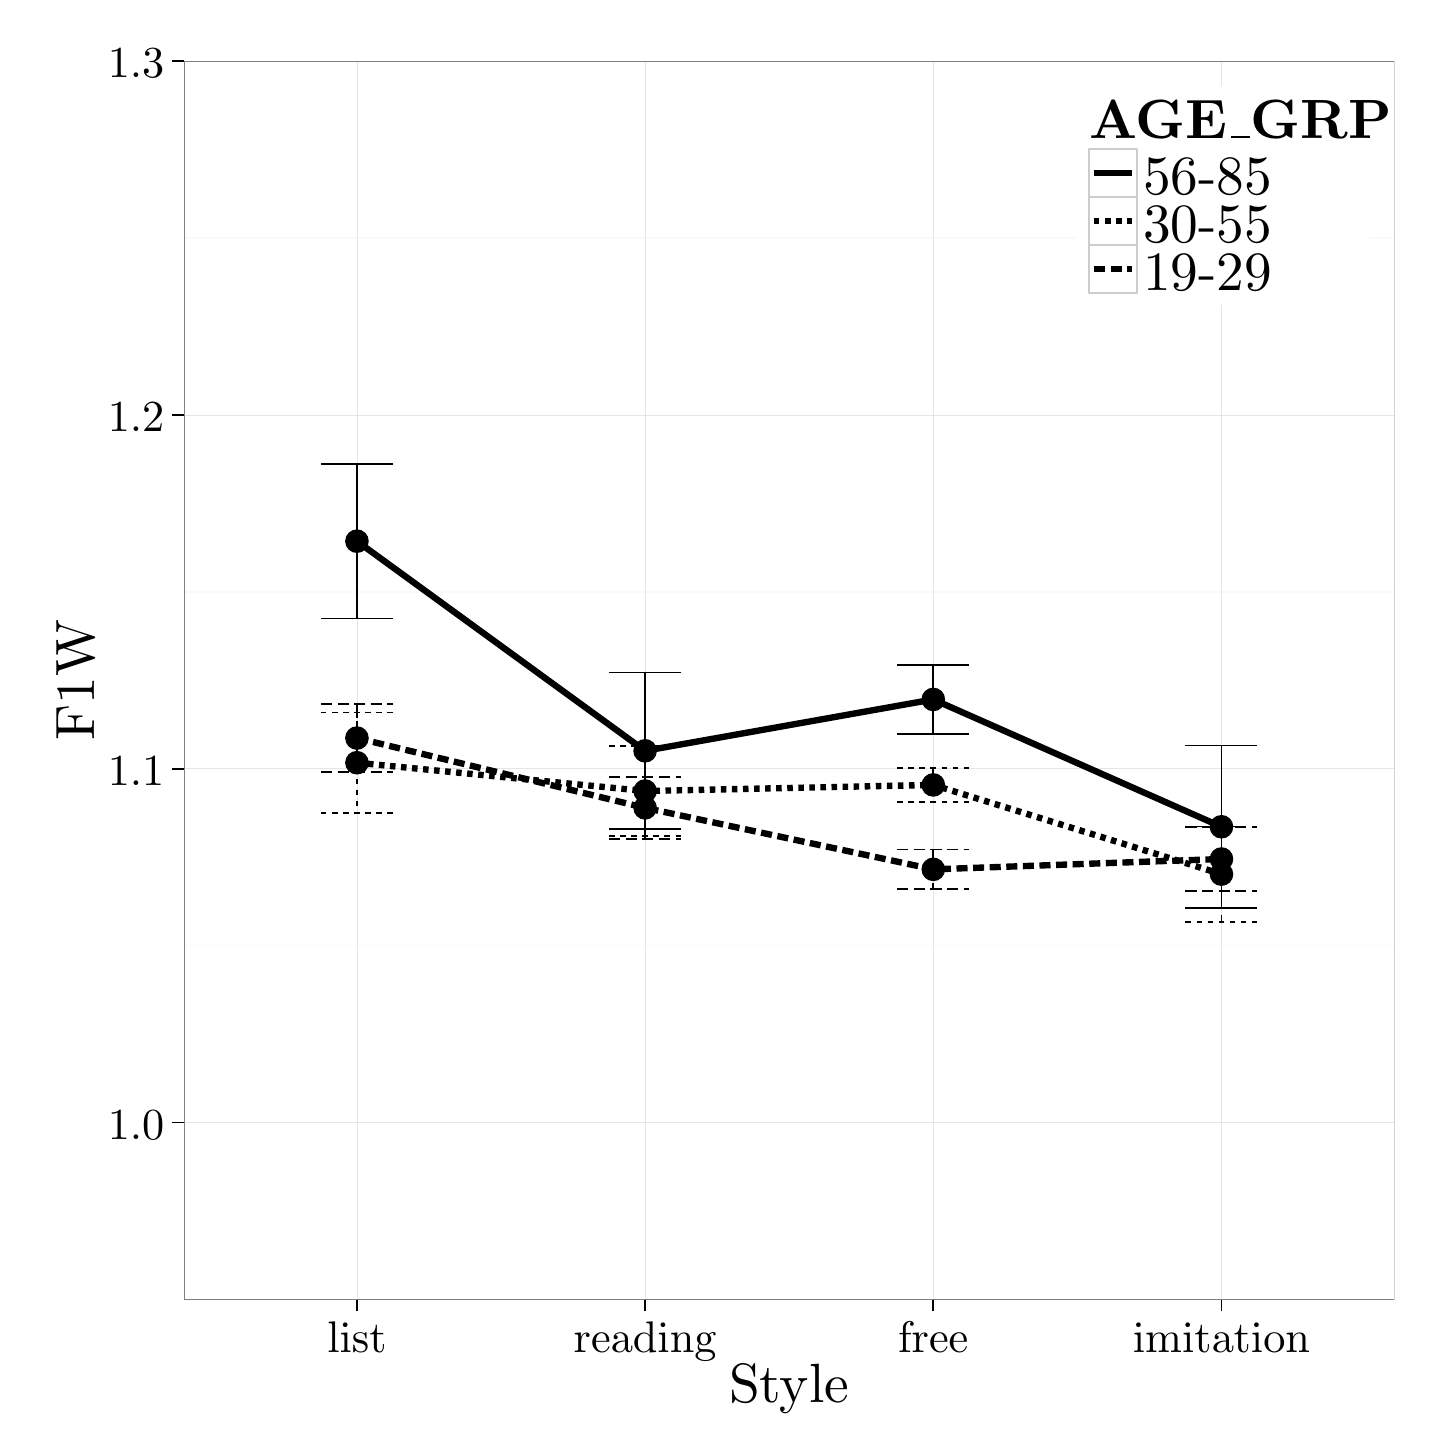
\begin{tikzpicture}[x=1pt,y=1pt]
\definecolor{fillColor}{RGB}{255,255,255}
\path[use as bounding box,fill=fillColor,fill opacity=0.00] (0,0) rectangle (505.89,505.89);
\begin{scope}
\path[clip] (  0.00,  0.00) rectangle (505.89,505.89);
\definecolor{drawColor}{RGB}{255,255,255}
\definecolor{fillColor}{RGB}{255,255,255}

\path[draw=drawColor,line width= 0.6pt,line join=round,line cap=round,fill=fillColor] (  0.00, -0.00) rectangle (505.89,505.89);
\end{scope}
\begin{scope}
\path[clip] ( 56.50, 46.31) rectangle (493.85,493.84);
\definecolor{fillColor}{RGB}{255,255,255}

\path[fill=fillColor] ( 56.50, 46.31) rectangle (493.85,493.84);
\definecolor{drawColor}{gray}{0.98}

\path[draw=drawColor,line width= 0.6pt,line join=round] ( 56.50, 46.31) --
	(493.85, 46.31);

\path[draw=drawColor,line width= 0.6pt,line join=round] ( 56.50,174.18) --
	(493.85,174.18);

\path[draw=drawColor,line width= 0.6pt,line join=round] ( 56.50,302.04) --
	(493.85,302.04);

\path[draw=drawColor,line width= 0.6pt,line join=round] ( 56.50,429.91) --
	(493.85,429.91);
\definecolor{drawColor}{gray}{0.90}

\path[draw=drawColor,line width= 0.2pt,line join=round] ( 56.50,110.24) --
	(493.85,110.24);

\path[draw=drawColor,line width= 0.2pt,line join=round] ( 56.50,238.11) --
	(493.85,238.11);

\path[draw=drawColor,line width= 0.2pt,line join=round] ( 56.50,365.98) --
	(493.85,365.98);

\path[draw=drawColor,line width= 0.2pt,line join=round] ( 56.50,493.84) --
	(493.85,493.84);

\path[draw=drawColor,line width= 0.2pt,line join=round] (118.98, 46.31) --
	(118.98,493.84);

\path[draw=drawColor,line width= 0.2pt,line join=round] (223.11, 46.31) --
	(223.11,493.84);

\path[draw=drawColor,line width= 0.2pt,line join=round] (327.24, 46.31) --
	(327.24,493.84);

\path[draw=drawColor,line width= 0.2pt,line join=round] (431.37, 46.31) --
	(431.37,493.84);
\definecolor{fillColor}{RGB}{0,0,0}

\path[fill=fillColor] (118.98,320.33) circle (  4.27);

\path[fill=fillColor] (118.98,240.28) circle (  4.27);

\path[fill=fillColor] (118.98,249.19) circle (  4.27);

\path[fill=fillColor] (223.11,244.58) circle (  4.27);

\path[fill=fillColor] (223.11,230.05) circle (  4.27);

\path[fill=fillColor] (223.11,223.96) circle (  4.27);

\path[fill=fillColor] (327.24,263.14) circle (  4.27);

\path[fill=fillColor] (327.24,232.25) circle (  4.27);

\path[fill=fillColor] (327.24,201.75) circle (  4.27);

\path[fill=fillColor] (431.37,217.13) circle (  4.27);

\path[fill=fillColor] (431.37,200.02) circle (  4.27);

\path[fill=fillColor] (431.37,205.49) circle (  4.27);
\definecolor{drawColor}{RGB}{0,0,0}

\path[draw=drawColor,line width= 2.3pt,line join=round] (118.98,320.33) --
	(223.11,244.58) --
	(327.24,263.14) --
	(431.37,217.13);

\path[draw=drawColor,line width= 2.3pt,dash pattern=on 2pt off 2pt ,line join=round] (118.98,240.28) --
	(223.11,230.05) --
	(327.24,232.25) --
	(431.37,200.02);

\path[draw=drawColor,line width= 2.3pt,dash pattern=on 4pt off 2pt ,line join=round] (118.98,249.19) --
	(223.11,223.96) --
	(327.24,201.75) --
	(431.37,205.49);

\path[draw=drawColor,line width= 0.6pt,line join=round] (105.96,348.22) --
	(132.00,348.22);

\path[draw=drawColor,line width= 0.6pt,line join=round] (118.98,348.22) --
	(118.98,292.43);

\path[draw=drawColor,line width= 0.6pt,line join=round] (105.96,292.43) --
	(132.00,292.43);

\path[draw=drawColor,line width= 0.6pt,line join=round] (210.09,272.92) --
	(236.13,272.92);

\path[draw=drawColor,line width= 0.6pt,line join=round] (223.11,272.92) --
	(223.11,216.23);

\path[draw=drawColor,line width= 0.6pt,line join=round] (210.09,216.23) --
	(236.13,216.23);

\path[draw=drawColor,line width= 0.6pt,line join=round] (314.22,275.63) --
	(340.25,275.63);

\path[draw=drawColor,line width= 0.6pt,line join=round] (327.24,275.63) --
	(327.24,250.64);

\path[draw=drawColor,line width= 0.6pt,line join=round] (314.22,250.64) --
	(340.25,250.64);

\path[draw=drawColor,line width= 0.6pt,line join=round] (418.35,246.47) --
	(444.38,246.47);

\path[draw=drawColor,line width= 0.6pt,line join=round] (431.37,246.47) --
	(431.37,187.78);

\path[draw=drawColor,line width= 0.6pt,line join=round] (418.35,187.78) --
	(444.38,187.78);

\path[draw=drawColor,line width= 0.6pt,dash pattern=on 2pt off 2pt ,line join=round] (105.96,258.48) --
	(132.00,258.48);

\path[draw=drawColor,line width= 0.6pt,dash pattern=on 2pt off 2pt ,line join=round] (118.98,258.48) --
	(118.98,222.08);

\path[draw=drawColor,line width= 0.6pt,dash pattern=on 2pt off 2pt ,line join=round] (105.96,222.08) --
	(132.00,222.08);

\path[draw=drawColor,line width= 0.6pt,dash pattern=on 2pt off 2pt ,line join=round] (210.09,246.30) --
	(236.13,246.30);

\path[draw=drawColor,line width= 0.6pt,dash pattern=on 2pt off 2pt ,line join=round] (223.11,246.30) --
	(223.11,213.79);

\path[draw=drawColor,line width= 0.6pt,dash pattern=on 2pt off 2pt ,line join=round] (210.09,213.79) --
	(236.13,213.79);

\path[draw=drawColor,line width= 0.6pt,dash pattern=on 2pt off 2pt ,line join=round] (314.22,238.34) --
	(340.25,238.34);

\path[draw=drawColor,line width= 0.6pt,dash pattern=on 2pt off 2pt ,line join=round] (327.24,238.34) --
	(327.24,226.17);

\path[draw=drawColor,line width= 0.6pt,dash pattern=on 2pt off 2pt ,line join=round] (314.22,226.17) --
	(340.25,226.17);

\path[draw=drawColor,line width= 0.6pt,dash pattern=on 2pt off 2pt ,line join=round] (418.35,217.26) --
	(444.38,217.26);

\path[draw=drawColor,line width= 0.6pt,dash pattern=on 2pt off 2pt ,line join=round] (431.37,217.26) --
	(431.37,182.77);

\path[draw=drawColor,line width= 0.6pt,dash pattern=on 2pt off 2pt ,line join=round] (418.35,182.77) --
	(444.38,182.77);

\path[draw=drawColor,line width= 0.6pt,dash pattern=on 4pt off 2pt ,line join=round] (105.96,261.52) --
	(132.00,261.52);

\path[draw=drawColor,line width= 0.6pt,dash pattern=on 4pt off 2pt ,line join=round] (118.98,261.52) --
	(118.98,236.86);

\path[draw=drawColor,line width= 0.6pt,dash pattern=on 4pt off 2pt ,line join=round] (105.96,236.86) --
	(132.00,236.86);

\path[draw=drawColor,line width= 0.6pt,dash pattern=on 4pt off 2pt ,line join=round] (210.09,235.23) --
	(236.13,235.23);

\path[draw=drawColor,line width= 0.6pt,dash pattern=on 4pt off 2pt ,line join=round] (223.11,235.23) --
	(223.11,212.68);

\path[draw=drawColor,line width= 0.6pt,dash pattern=on 4pt off 2pt ,line join=round] (210.09,212.68) --
	(236.13,212.68);

\path[draw=drawColor,line width= 0.6pt,dash pattern=on 4pt off 2pt ,line join=round] (314.22,208.95) --
	(340.25,208.95);

\path[draw=drawColor,line width= 0.6pt,dash pattern=on 4pt off 2pt ,line join=round] (327.24,208.95) --
	(327.24,194.55);

\path[draw=drawColor,line width= 0.6pt,dash pattern=on 4pt off 2pt ,line join=round] (314.22,194.55) --
	(340.25,194.55);

\path[draw=drawColor,line width= 0.6pt,dash pattern=on 4pt off 2pt ,line join=round] (418.35,217.02) --
	(444.38,217.02);

\path[draw=drawColor,line width= 0.6pt,dash pattern=on 4pt off 2pt ,line join=round] (431.37,217.02) --
	(431.37,193.96);

\path[draw=drawColor,line width= 0.6pt,dash pattern=on 4pt off 2pt ,line join=round] (418.35,193.96) --
	(444.38,193.96);
\definecolor{drawColor}{gray}{0.50}

\path[draw=drawColor,line width= 0.6pt,line join=round,line cap=round] ( 56.50, 46.31) rectangle (493.85,493.84);
\end{scope}
\begin{scope}
\path[clip] (  0.00,  0.00) rectangle (505.89,505.89);
\definecolor{drawColor}{RGB}{0,0,0}

\node[text=drawColor,anchor=base east,inner sep=0pt, outer sep=0pt, scale=  1.60] at ( 49.39,104.21) {1.0};

\node[text=drawColor,anchor=base east,inner sep=0pt, outer sep=0pt, scale=  1.60] at ( 49.39,232.08) {1.1};

\node[text=drawColor,anchor=base east,inner sep=0pt, outer sep=0pt, scale=  1.60] at ( 49.39,359.94) {1.2};

\node[text=drawColor,anchor=base east,inner sep=0pt, outer sep=0pt, scale=  1.60] at ( 49.39,487.81) {1.3};
\end{scope}
\begin{scope}
\path[clip] (  0.00,  0.00) rectangle (505.89,505.89);
\definecolor{drawColor}{RGB}{0,0,0}

\path[draw=drawColor,line width= 0.6pt,line join=round] ( 52.24,110.24) --
	( 56.50,110.24);

\path[draw=drawColor,line width= 0.6pt,line join=round] ( 52.24,238.11) --
	( 56.50,238.11);

\path[draw=drawColor,line width= 0.6pt,line join=round] ( 52.24,365.98) --
	( 56.50,365.98);

\path[draw=drawColor,line width= 0.6pt,line join=round] ( 52.24,493.84) --
	( 56.50,493.84);
\end{scope}
\begin{scope}
\path[clip] (  0.00,  0.00) rectangle (505.89,505.89);
\definecolor{drawColor}{RGB}{0,0,0}

\path[draw=drawColor,line width= 0.6pt,line join=round] (118.98, 42.04) --
	(118.98, 46.31);

\path[draw=drawColor,line width= 0.6pt,line join=round] (223.11, 42.04) --
	(223.11, 46.31);

\path[draw=drawColor,line width= 0.6pt,line join=round] (327.24, 42.04) --
	(327.24, 46.31);

\path[draw=drawColor,line width= 0.6pt,line join=round] (431.37, 42.04) --
	(431.37, 46.31);
\end{scope}
\begin{scope}
\path[clip] (  0.00,  0.00) rectangle (505.89,505.89);
\definecolor{drawColor}{RGB}{0,0,0}

\node[text=drawColor,anchor=base,inner sep=0pt, outer sep=0pt, scale=  1.60] at (118.98, 27.13) {list};

\node[text=drawColor,anchor=base,inner sep=0pt, outer sep=0pt, scale=  1.60] at (223.11, 27.13) {reading};

\node[text=drawColor,anchor=base,inner sep=0pt, outer sep=0pt, scale=  1.60] at (327.24, 27.13) {free};

\node[text=drawColor,anchor=base,inner sep=0pt, outer sep=0pt, scale=  1.60] at (431.37, 27.13) {imitation};
\end{scope}
\begin{scope}
\path[clip] (  0.00,  0.00) rectangle (505.89,505.89);
\definecolor{drawColor}{RGB}{0,0,0}

\node[text=drawColor,anchor=base,inner sep=0pt, outer sep=0pt, scale=  2.00] at (275.17,  9.03) {Style};
\end{scope}
\begin{scope}
\path[clip] (  0.00,  0.00) rectangle (505.89,505.89);
\definecolor{drawColor}{RGB}{0,0,0}

\node[text=drawColor,rotate= 90.00,anchor=base,inner sep=0pt, outer sep=0pt, scale=  2.00] at ( 24.12,270.08) {F1W};
\end{scope}
\begin{scope}
\path[clip] (  0.00,  0.00) rectangle (505.89,505.89);
\definecolor{fillColor}{RGB}{255,255,255}

\path[fill=fillColor] (379.28,405.66) rectangle (484.98,484.98);
\end{scope}
\begin{scope}
\path[clip] (  0.00,  0.00) rectangle (505.89,505.89);
\definecolor{drawColor}{RGB}{0,0,0}

\node[text=drawColor,anchor=base west,inner sep=0pt, outer sep=0pt, scale=  2.00] at (383.55,465.96) {\bfseries AGE{\_{}}GRP};
\end{scope}
\begin{scope}
\path[clip] (  0.00,  0.00) rectangle (505.89,505.89);
\definecolor{drawColor}{gray}{0.80}
\definecolor{fillColor}{RGB}{255,255,255}

\path[draw=drawColor,line width= 0.6pt,line join=round,line cap=round,fill=fillColor] (383.55,444.61) rectangle (400.89,461.96);
\end{scope}
\begin{scope}
\path[clip] (  0.00,  0.00) rectangle (505.89,505.89);
\definecolor{drawColor}{RGB}{0,0,0}

\path[draw=drawColor,line width= 2.3pt,line join=round] (385.28,453.29) -- (399.16,453.29);
\end{scope}
\begin{scope}
\path[clip] (  0.00,  0.00) rectangle (505.89,505.89);
\definecolor{drawColor}{RGB}{0,0,0}

\path[draw=drawColor,line width= 0.6pt,line join=round] (385.28,453.29) -- (399.16,453.29);
\end{scope}
\begin{scope}
\path[clip] (  0.00,  0.00) rectangle (505.89,505.89);
\definecolor{drawColor}{gray}{0.80}
\definecolor{fillColor}{RGB}{255,255,255}

\path[draw=drawColor,line width= 0.6pt,line join=round,line cap=round,fill=fillColor] (383.55,427.27) rectangle (400.89,444.61);
\end{scope}
\begin{scope}
\path[clip] (  0.00,  0.00) rectangle (505.89,505.89);
\definecolor{drawColor}{RGB}{0,0,0}

\path[draw=drawColor,line width= 2.3pt,dash pattern=on 2pt off 2pt ,line join=round] (385.28,435.94) -- (399.16,435.94);
\end{scope}
\begin{scope}
\path[clip] (  0.00,  0.00) rectangle (505.89,505.89);
\definecolor{drawColor}{RGB}{0,0,0}

\path[draw=drawColor,line width= 0.6pt,dash pattern=on 2pt off 2pt ,line join=round] (385.28,435.94) -- (399.16,435.94);
\end{scope}
\begin{scope}
\path[clip] (  0.00,  0.00) rectangle (505.89,505.89);
\definecolor{drawColor}{gray}{0.80}
\definecolor{fillColor}{RGB}{255,255,255}

\path[draw=drawColor,line width= 0.6pt,line join=round,line cap=round,fill=fillColor] (383.55,409.92) rectangle (400.89,427.27);
\end{scope}
\begin{scope}
\path[clip] (  0.00,  0.00) rectangle (505.89,505.89);
\definecolor{drawColor}{RGB}{0,0,0}

\path[draw=drawColor,line width= 2.3pt,dash pattern=on 4pt off 2pt ,line join=round] (385.28,418.60) -- (399.16,418.60);
\end{scope}
\begin{scope}
\path[clip] (  0.00,  0.00) rectangle (505.89,505.89);
\definecolor{drawColor}{RGB}{0,0,0}

\path[draw=drawColor,line width= 0.6pt,dash pattern=on 4pt off 2pt ,line join=round] (385.28,418.60) -- (399.16,418.60);
\end{scope}
\begin{scope}
\path[clip] (  0.00,  0.00) rectangle (505.89,505.89);
\definecolor{drawColor}{RGB}{0,0,0}

\node[text=drawColor,anchor=base west,inner sep=0pt, outer sep=0pt, scale=  2.00] at (403.06,445.75) {56-85};
\end{scope}
\begin{scope}
\path[clip] (  0.00,  0.00) rectangle (505.89,505.89);
\definecolor{drawColor}{RGB}{0,0,0}

\node[text=drawColor,anchor=base west,inner sep=0pt, outer sep=0pt, scale=  2.00] at (403.06,428.40) {30-55};
\end{scope}
\begin{scope}
\path[clip] (  0.00,  0.00) rectangle (505.89,505.89);
\definecolor{drawColor}{RGB}{0,0,0}

\node[text=drawColor,anchor=base west,inner sep=0pt, outer sep=0pt, scale=  2.00] at (403.06,411.06) {19-29};
\end{scope}
\end{tikzpicture}
} 
	\caption{\textsc{nurse} (F1) by style and age}
	\label{fig.line.f1.nurse.tot}
\end{figure}

Figure \ref{fig.line.f1.nurse.tot}, which is based on the complete data set of \textsc{nurse} observations, shows that differences between age groups are not really drastic.
The young and the middle group have virtually identical values in three out of four speaking styles, only the oldest speakers are slightly more distinct\is{distinctness}.
However, even that is mostly true for the word list.
While reading a text and during accent perform\is{accent performance}ance all three groups have comparable F1 measurements.
Only in spontaneous speech (which accounts for the clear majority of observations and therefore explains the results visualised in Figure \ref{fig.box.f1.nurse.tot}) do all three groups have significantly different F1 means.
No group shows systematic and significant style variation (note the often overlapping standard error bars between styles).
Especially the lines of the young and middle-aged speakers look pretty level.
If anything, \isi{style shifting} can be found in the oldest participants, where there seems to be a more systematic downward trend from the left of the graph to the right (although the mean of `reading' is a little off in this respect).
However, just as in the other groups, the line potentially has a `wrong' negative slope.
If we were looking at Labovian \isi{style shifting}, we would expect an \emph{upward} slope, i.e. \textsc{nurse} realisations becoming \emph{more} Scouse from the word list to imitation\is{accent performance}, instead of the opposite.

\begin{figure}[h!]
	\centering
	\begin{subfigure}{.49\textwidth}
		\centering
			\definecolor{shadecolor}{rgb}{0.969, 0.969, 0.969}
			\resizebox{\linewidth}{!}{% Created by tikzDevice version 0.8.1 on 2016-02-09 02:14:47
% !TEX encoding = UTF-8 Unicode
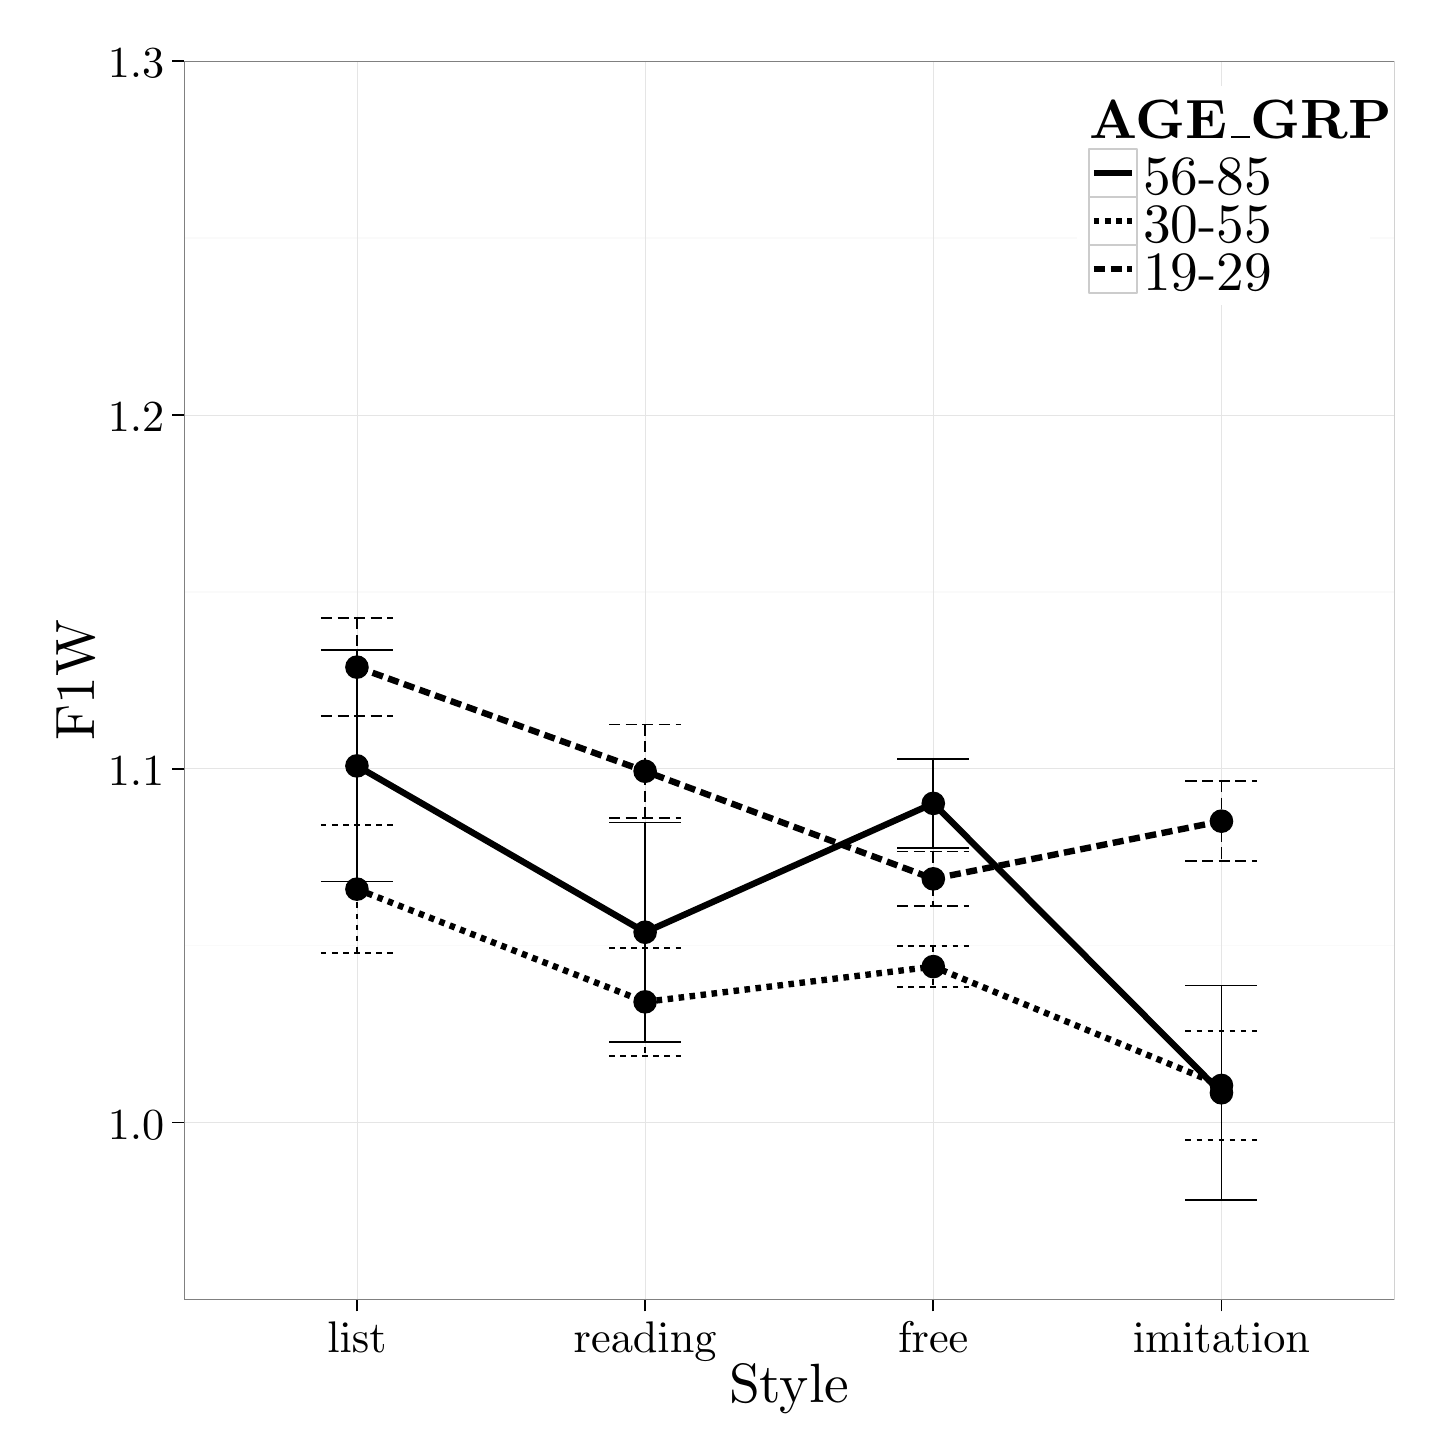
\begin{tikzpicture}[x=1pt,y=1pt]
\definecolor{fillColor}{RGB}{255,255,255}
\path[use as bounding box,fill=fillColor,fill opacity=0.00] (0,0) rectangle (505.89,505.89);
\begin{scope}
\path[clip] (  0.00,  0.00) rectangle (505.89,505.89);
\definecolor{drawColor}{RGB}{255,255,255}
\definecolor{fillColor}{RGB}{255,255,255}

\path[draw=drawColor,line width= 0.6pt,line join=round,line cap=round,fill=fillColor] (  0.00, -0.00) rectangle (505.89,505.89);
\end{scope}
\begin{scope}
\path[clip] ( 56.50, 46.31) rectangle (493.85,493.84);
\definecolor{fillColor}{RGB}{255,255,255}

\path[fill=fillColor] ( 56.50, 46.31) rectangle (493.85,493.84);
\definecolor{drawColor}{gray}{0.98}

\path[draw=drawColor,line width= 0.6pt,line join=round] ( 56.50, 46.31) --
	(493.85, 46.31);

\path[draw=drawColor,line width= 0.6pt,line join=round] ( 56.50,174.18) --
	(493.85,174.18);

\path[draw=drawColor,line width= 0.6pt,line join=round] ( 56.50,302.04) --
	(493.85,302.04);

\path[draw=drawColor,line width= 0.6pt,line join=round] ( 56.50,429.91) --
	(493.85,429.91);
\definecolor{drawColor}{gray}{0.90}

\path[draw=drawColor,line width= 0.2pt,line join=round] ( 56.50,110.24) --
	(493.85,110.24);

\path[draw=drawColor,line width= 0.2pt,line join=round] ( 56.50,238.11) --
	(493.85,238.11);

\path[draw=drawColor,line width= 0.2pt,line join=round] ( 56.50,365.98) --
	(493.85,365.98);

\path[draw=drawColor,line width= 0.2pt,line join=round] ( 56.50,493.84) --
	(493.85,493.84);

\path[draw=drawColor,line width= 0.2pt,line join=round] (118.98, 46.31) --
	(118.98,493.84);

\path[draw=drawColor,line width= 0.2pt,line join=round] (223.11, 46.31) --
	(223.11,493.84);

\path[draw=drawColor,line width= 0.2pt,line join=round] (327.24, 46.31) --
	(327.24,493.84);

\path[draw=drawColor,line width= 0.2pt,line join=round] (431.37, 46.31) --
	(431.37,493.84);
\definecolor{fillColor}{RGB}{0,0,0}

\path[fill=fillColor] (118.98,239.13) circle (  4.27);

\path[fill=fillColor] (118.98,194.60) circle (  4.27);

\path[fill=fillColor] (118.98,274.82) circle (  4.27);

\path[fill=fillColor] (223.11,179.03) circle (  4.27);

\path[fill=fillColor] (223.11,153.87) circle (  4.27);

\path[fill=fillColor] (223.11,237.20) circle (  4.27);

\path[fill=fillColor] (327.24,225.58) circle (  4.27);

\path[fill=fillColor] (327.24,166.60) circle (  4.27);

\path[fill=fillColor] (327.24,198.32) circle (  4.27);

\path[fill=fillColor] (431.37,121.01) circle (  4.27);

\path[fill=fillColor] (431.37,123.67) circle (  4.27);

\path[fill=fillColor] (431.37,219.16) circle (  4.27);
\definecolor{drawColor}{RGB}{0,0,0}

\path[draw=drawColor,line width= 2.3pt,line join=round] (118.98,239.13) --
	(223.11,179.03) --
	(327.24,225.58) --
	(431.37,121.01);

\path[draw=drawColor,line width= 2.3pt,dash pattern=on 2pt off 2pt ,line join=round] (118.98,194.60) --
	(223.11,153.87) --
	(327.24,166.60) --
	(431.37,123.67);

\path[draw=drawColor,line width= 2.3pt,dash pattern=on 4pt off 2pt ,line join=round] (118.98,274.82) --
	(223.11,237.20) --
	(327.24,198.32) --
	(431.37,219.16);

\path[draw=drawColor,line width= 0.6pt,line join=round] (105.96,280.93) --
	(132.00,280.93);

\path[draw=drawColor,line width= 0.6pt,line join=round] (118.98,280.93) --
	(118.98,197.33);

\path[draw=drawColor,line width= 0.6pt,line join=round] (105.96,197.33) --
	(132.00,197.33);

\path[draw=drawColor,line width= 0.6pt,line join=round] (210.09,218.62) --
	(236.13,218.62);

\path[draw=drawColor,line width= 0.6pt,line join=round] (223.11,218.62) --
	(223.11,139.45);

\path[draw=drawColor,line width= 0.6pt,line join=round] (210.09,139.45) --
	(236.13,139.45);

\path[draw=drawColor,line width= 0.6pt,line join=round] (314.22,241.73) --
	(340.25,241.73);

\path[draw=drawColor,line width= 0.6pt,line join=round] (327.24,241.73) --
	(327.24,209.43);

\path[draw=drawColor,line width= 0.6pt,line join=round] (314.22,209.43) --
	(340.25,209.43);

\path[draw=drawColor,line width= 0.6pt,line join=round] (418.35,159.76) --
	(444.38,159.76);

\path[draw=drawColor,line width= 0.6pt,line join=round] (431.37,159.76) --
	(431.37, 82.26);

\path[draw=drawColor,line width= 0.6pt,line join=round] (418.35, 82.26) --
	(444.38, 82.26);

\path[draw=drawColor,line width= 0.6pt,dash pattern=on 2pt off 2pt ,line join=round] (105.96,217.78) --
	(132.00,217.78);

\path[draw=drawColor,line width= 0.6pt,dash pattern=on 2pt off 2pt ,line join=round] (118.98,217.78) --
	(118.98,171.42);

\path[draw=drawColor,line width= 0.6pt,dash pattern=on 2pt off 2pt ,line join=round] (105.96,171.42) --
	(132.00,171.42);

\path[draw=drawColor,line width= 0.6pt,dash pattern=on 2pt off 2pt ,line join=round] (210.09,173.39) --
	(236.13,173.39);

\path[draw=drawColor,line width= 0.6pt,dash pattern=on 2pt off 2pt ,line join=round] (223.11,173.39) --
	(223.11,134.36);

\path[draw=drawColor,line width= 0.6pt,dash pattern=on 2pt off 2pt ,line join=round] (210.09,134.36) --
	(236.13,134.36);

\path[draw=drawColor,line width= 0.6pt,dash pattern=on 2pt off 2pt ,line join=round] (314.22,174.02) --
	(340.25,174.02);

\path[draw=drawColor,line width= 0.6pt,dash pattern=on 2pt off 2pt ,line join=round] (327.24,174.02) --
	(327.24,159.18);

\path[draw=drawColor,line width= 0.6pt,dash pattern=on 2pt off 2pt ,line join=round] (314.22,159.18) --
	(340.25,159.18);

\path[draw=drawColor,line width= 0.6pt,dash pattern=on 2pt off 2pt ,line join=round] (418.35,143.37) --
	(444.38,143.37);

\path[draw=drawColor,line width= 0.6pt,dash pattern=on 2pt off 2pt ,line join=round] (431.37,143.37) --
	(431.37,103.96);

\path[draw=drawColor,line width= 0.6pt,dash pattern=on 2pt off 2pt ,line join=round] (418.35,103.96) --
	(444.38,103.96);

\path[draw=drawColor,line width= 0.6pt,dash pattern=on 4pt off 2pt ,line join=round] (105.96,292.51) --
	(132.00,292.51);

\path[draw=drawColor,line width= 0.6pt,dash pattern=on 4pt off 2pt ,line join=round] (118.98,292.51) --
	(118.98,257.13);

\path[draw=drawColor,line width= 0.6pt,dash pattern=on 4pt off 2pt ,line join=round] (105.96,257.13) --
	(132.00,257.13);

\path[draw=drawColor,line width= 0.6pt,dash pattern=on 4pt off 2pt ,line join=round] (210.09,254.10) --
	(236.13,254.10);

\path[draw=drawColor,line width= 0.6pt,dash pattern=on 4pt off 2pt ,line join=round] (223.11,254.10) --
	(223.11,220.30);

\path[draw=drawColor,line width= 0.6pt,dash pattern=on 4pt off 2pt ,line join=round] (210.09,220.30) --
	(236.13,220.30);

\path[draw=drawColor,line width= 0.6pt,dash pattern=on 4pt off 2pt ,line join=round] (314.22,208.19) --
	(340.25,208.19);

\path[draw=drawColor,line width= 0.6pt,dash pattern=on 4pt off 2pt ,line join=round] (327.24,208.19) --
	(327.24,188.45);

\path[draw=drawColor,line width= 0.6pt,dash pattern=on 4pt off 2pt ,line join=round] (314.22,188.45) --
	(340.25,188.45);

\path[draw=drawColor,line width= 0.6pt,dash pattern=on 4pt off 2pt ,line join=round] (418.35,233.65) --
	(444.38,233.65);

\path[draw=drawColor,line width= 0.6pt,dash pattern=on 4pt off 2pt ,line join=round] (431.37,233.65) --
	(431.37,204.67);

\path[draw=drawColor,line width= 0.6pt,dash pattern=on 4pt off 2pt ,line join=round] (418.35,204.67) --
	(444.38,204.67);
\definecolor{drawColor}{gray}{0.50}

\path[draw=drawColor,line width= 0.6pt,line join=round,line cap=round] ( 56.50, 46.31) rectangle (493.85,493.84);
\end{scope}
\begin{scope}
\path[clip] (  0.00,  0.00) rectangle (505.89,505.89);
\definecolor{drawColor}{RGB}{0,0,0}

\node[text=drawColor,anchor=base east,inner sep=0pt, outer sep=0pt, scale=  1.60] at ( 49.39,104.21) {1.0};

\node[text=drawColor,anchor=base east,inner sep=0pt, outer sep=0pt, scale=  1.60] at ( 49.39,232.08) {1.1};

\node[text=drawColor,anchor=base east,inner sep=0pt, outer sep=0pt, scale=  1.60] at ( 49.39,359.94) {1.2};

\node[text=drawColor,anchor=base east,inner sep=0pt, outer sep=0pt, scale=  1.60] at ( 49.39,487.81) {1.3};
\end{scope}
\begin{scope}
\path[clip] (  0.00,  0.00) rectangle (505.89,505.89);
\definecolor{drawColor}{RGB}{0,0,0}

\path[draw=drawColor,line width= 0.6pt,line join=round] ( 52.24,110.24) --
	( 56.50,110.24);

\path[draw=drawColor,line width= 0.6pt,line join=round] ( 52.24,238.11) --
	( 56.50,238.11);

\path[draw=drawColor,line width= 0.6pt,line join=round] ( 52.24,365.98) --
	( 56.50,365.98);

\path[draw=drawColor,line width= 0.6pt,line join=round] ( 52.24,493.84) --
	( 56.50,493.84);
\end{scope}
\begin{scope}
\path[clip] (  0.00,  0.00) rectangle (505.89,505.89);
\definecolor{drawColor}{RGB}{0,0,0}

\path[draw=drawColor,line width= 0.6pt,line join=round] (118.98, 42.04) --
	(118.98, 46.31);

\path[draw=drawColor,line width= 0.6pt,line join=round] (223.11, 42.04) --
	(223.11, 46.31);

\path[draw=drawColor,line width= 0.6pt,line join=round] (327.24, 42.04) --
	(327.24, 46.31);

\path[draw=drawColor,line width= 0.6pt,line join=round] (431.37, 42.04) --
	(431.37, 46.31);
\end{scope}
\begin{scope}
\path[clip] (  0.00,  0.00) rectangle (505.89,505.89);
\definecolor{drawColor}{RGB}{0,0,0}

\node[text=drawColor,anchor=base,inner sep=0pt, outer sep=0pt, scale=  1.60] at (118.98, 27.13) {list};

\node[text=drawColor,anchor=base,inner sep=0pt, outer sep=0pt, scale=  1.60] at (223.11, 27.13) {reading};

\node[text=drawColor,anchor=base,inner sep=0pt, outer sep=0pt, scale=  1.60] at (327.24, 27.13) {free};

\node[text=drawColor,anchor=base,inner sep=0pt, outer sep=0pt, scale=  1.60] at (431.37, 27.13) {imitation};
\end{scope}
\begin{scope}
\path[clip] (  0.00,  0.00) rectangle (505.89,505.89);
\definecolor{drawColor}{RGB}{0,0,0}

\node[text=drawColor,anchor=base,inner sep=0pt, outer sep=0pt, scale=  2.00] at (275.17,  9.03) {Style};
\end{scope}
\begin{scope}
\path[clip] (  0.00,  0.00) rectangle (505.89,505.89);
\definecolor{drawColor}{RGB}{0,0,0}

\node[text=drawColor,rotate= 90.00,anchor=base,inner sep=0pt, outer sep=0pt, scale=  2.00] at ( 24.12,270.08) {F1W};
\end{scope}
\begin{scope}
\path[clip] (  0.00,  0.00) rectangle (505.89,505.89);
\definecolor{fillColor}{RGB}{255,255,255}

\path[fill=fillColor] (379.28,405.66) rectangle (484.98,484.98);
\end{scope}
\begin{scope}
\path[clip] (  0.00,  0.00) rectangle (505.89,505.89);
\definecolor{drawColor}{RGB}{0,0,0}

\node[text=drawColor,anchor=base west,inner sep=0pt, outer sep=0pt, scale=  2.00] at (383.55,465.96) {\bfseries AGE{\_{}}GRP};
\end{scope}
\begin{scope}
\path[clip] (  0.00,  0.00) rectangle (505.89,505.89);
\definecolor{drawColor}{gray}{0.80}
\definecolor{fillColor}{RGB}{255,255,255}

\path[draw=drawColor,line width= 0.6pt,line join=round,line cap=round,fill=fillColor] (383.55,444.61) rectangle (400.89,461.96);
\end{scope}
\begin{scope}
\path[clip] (  0.00,  0.00) rectangle (505.89,505.89);
\definecolor{drawColor}{RGB}{0,0,0}

\path[draw=drawColor,line width= 2.3pt,line join=round] (385.28,453.29) -- (399.16,453.29);
\end{scope}
\begin{scope}
\path[clip] (  0.00,  0.00) rectangle (505.89,505.89);
\definecolor{drawColor}{RGB}{0,0,0}

\path[draw=drawColor,line width= 0.6pt,line join=round] (385.28,453.29) -- (399.16,453.29);
\end{scope}
\begin{scope}
\path[clip] (  0.00,  0.00) rectangle (505.89,505.89);
\definecolor{drawColor}{gray}{0.80}
\definecolor{fillColor}{RGB}{255,255,255}

\path[draw=drawColor,line width= 0.6pt,line join=round,line cap=round,fill=fillColor] (383.55,427.27) rectangle (400.89,444.61);
\end{scope}
\begin{scope}
\path[clip] (  0.00,  0.00) rectangle (505.89,505.89);
\definecolor{drawColor}{RGB}{0,0,0}

\path[draw=drawColor,line width= 2.3pt,dash pattern=on 2pt off 2pt ,line join=round] (385.28,435.94) -- (399.16,435.94);
\end{scope}
\begin{scope}
\path[clip] (  0.00,  0.00) rectangle (505.89,505.89);
\definecolor{drawColor}{RGB}{0,0,0}

\path[draw=drawColor,line width= 0.6pt,dash pattern=on 2pt off 2pt ,line join=round] (385.28,435.94) -- (399.16,435.94);
\end{scope}
\begin{scope}
\path[clip] (  0.00,  0.00) rectangle (505.89,505.89);
\definecolor{drawColor}{gray}{0.80}
\definecolor{fillColor}{RGB}{255,255,255}

\path[draw=drawColor,line width= 0.6pt,line join=round,line cap=round,fill=fillColor] (383.55,409.92) rectangle (400.89,427.27);
\end{scope}
\begin{scope}
\path[clip] (  0.00,  0.00) rectangle (505.89,505.89);
\definecolor{drawColor}{RGB}{0,0,0}

\path[draw=drawColor,line width= 2.3pt,dash pattern=on 4pt off 2pt ,line join=round] (385.28,418.60) -- (399.16,418.60);
\end{scope}
\begin{scope}
\path[clip] (  0.00,  0.00) rectangle (505.89,505.89);
\definecolor{drawColor}{RGB}{0,0,0}

\path[draw=drawColor,line width= 0.6pt,dash pattern=on 4pt off 2pt ,line join=round] (385.28,418.60) -- (399.16,418.60);
\end{scope}
\begin{scope}
\path[clip] (  0.00,  0.00) rectangle (505.89,505.89);
\definecolor{drawColor}{RGB}{0,0,0}

\node[text=drawColor,anchor=base west,inner sep=0pt, outer sep=0pt, scale=  2.00] at (403.06,445.75) {56-85};
\end{scope}
\begin{scope}
\path[clip] (  0.00,  0.00) rectangle (505.89,505.89);
\definecolor{drawColor}{RGB}{0,0,0}

\node[text=drawColor,anchor=base west,inner sep=0pt, outer sep=0pt, scale=  2.00] at (403.06,428.40) {30-55};
\end{scope}
\begin{scope}
\path[clip] (  0.00,  0.00) rectangle (505.89,505.89);
\definecolor{drawColor}{RGB}{0,0,0}

\node[text=drawColor,anchor=base west,inner sep=0pt, outer sep=0pt, scale=  2.00] at (403.06,411.06) {19-29};
\end{scope}
\end{tikzpicture}
} 
		\caption{women}
		\label{fig.line.f1.nurse.women}
	\end{subfigure}
	\begin{subfigure}{.49\textwidth}
		\centering
			\definecolor{shadecolor}{rgb}{0.969, 0.969, 0.969}
			\resizebox{\linewidth}{!}{% Created by tikzDevice version 0.8.1 on 2016-02-09 02:14:48
% !TEX encoding = UTF-8 Unicode
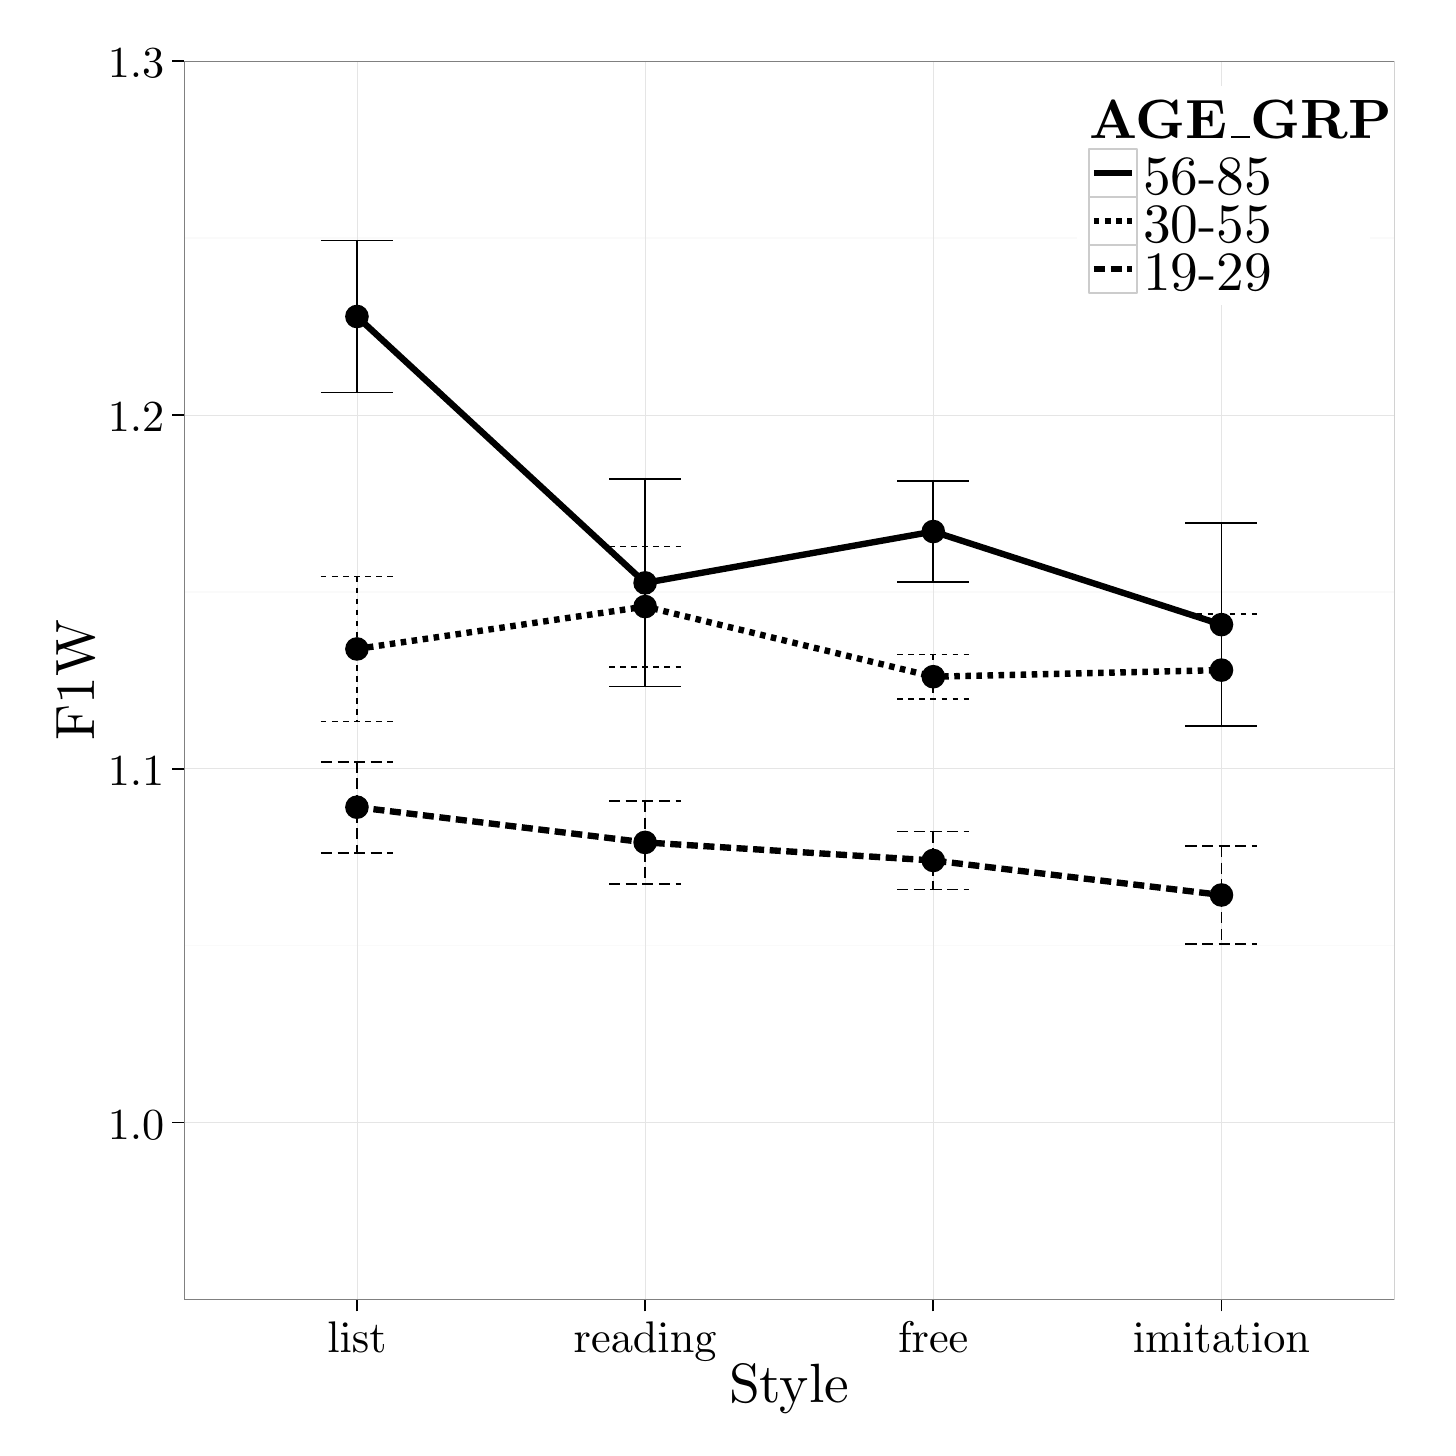
\begin{tikzpicture}[x=1pt,y=1pt]
\definecolor{fillColor}{RGB}{255,255,255}
\path[use as bounding box,fill=fillColor,fill opacity=0.00] (0,0) rectangle (505.89,505.89);
\begin{scope}
\path[clip] (  0.00,  0.00) rectangle (505.89,505.89);
\definecolor{drawColor}{RGB}{255,255,255}
\definecolor{fillColor}{RGB}{255,255,255}

\path[draw=drawColor,line width= 0.6pt,line join=round,line cap=round,fill=fillColor] (  0.00, -0.00) rectangle (505.89,505.89);
\end{scope}
\begin{scope}
\path[clip] ( 56.50, 46.31) rectangle (493.85,493.84);
\definecolor{fillColor}{RGB}{255,255,255}

\path[fill=fillColor] ( 56.50, 46.31) rectangle (493.85,493.84);
\definecolor{drawColor}{gray}{0.98}

\path[draw=drawColor,line width= 0.6pt,line join=round] ( 56.50, 46.31) --
	(493.85, 46.31);

\path[draw=drawColor,line width= 0.6pt,line join=round] ( 56.50,174.18) --
	(493.85,174.18);

\path[draw=drawColor,line width= 0.6pt,line join=round] ( 56.50,302.04) --
	(493.85,302.04);

\path[draw=drawColor,line width= 0.6pt,line join=round] ( 56.50,429.91) --
	(493.85,429.91);
\definecolor{drawColor}{gray}{0.90}

\path[draw=drawColor,line width= 0.2pt,line join=round] ( 56.50,110.24) --
	(493.85,110.24);

\path[draw=drawColor,line width= 0.2pt,line join=round] ( 56.50,238.11) --
	(493.85,238.11);

\path[draw=drawColor,line width= 0.2pt,line join=round] ( 56.50,365.98) --
	(493.85,365.98);

\path[draw=drawColor,line width= 0.2pt,line join=round] ( 56.50,493.84) --
	(493.85,493.84);

\path[draw=drawColor,line width= 0.2pt,line join=round] (118.98, 46.31) --
	(118.98,493.84);

\path[draw=drawColor,line width= 0.2pt,line join=round] (223.11, 46.31) --
	(223.11,493.84);

\path[draw=drawColor,line width= 0.2pt,line join=round] (327.24, 46.31) --
	(327.24,493.84);

\path[draw=drawColor,line width= 0.2pt,line join=round] (431.37, 46.31) --
	(431.37,493.84);
\definecolor{fillColor}{RGB}{0,0,0}

\path[fill=fillColor] (118.98,401.52) circle (  4.27);

\path[fill=fillColor] (118.98,281.39) circle (  4.27);

\path[fill=fillColor] (118.98,224.21) circle (  4.27);

\path[fill=fillColor] (223.11,305.26) circle (  4.27);

\path[fill=fillColor] (223.11,296.70) circle (  4.27);

\path[fill=fillColor] (223.11,211.48) circle (  4.27);

\path[fill=fillColor] (327.24,323.81) circle (  4.27);

\path[fill=fillColor] (327.24,271.36) circle (  4.27);

\path[fill=fillColor] (327.24,204.95) circle (  4.27);

\path[fill=fillColor] (431.37,290.18) circle (  4.27);

\path[fill=fillColor] (431.37,273.74) circle (  4.27);

\path[fill=fillColor] (431.37,192.48) circle (  4.27);
\definecolor{drawColor}{RGB}{0,0,0}

\path[draw=drawColor,line width= 2.3pt,line join=round] (118.98,401.52) --
	(223.11,305.26) --
	(327.24,323.81) --
	(431.37,290.18);

\path[draw=drawColor,line width= 2.3pt,dash pattern=on 2pt off 2pt ,line join=round] (118.98,281.39) --
	(223.11,296.70) --
	(327.24,271.36) --
	(431.37,273.74);

\path[draw=drawColor,line width= 2.3pt,dash pattern=on 4pt off 2pt ,line join=round] (118.98,224.21) --
	(223.11,211.48) --
	(327.24,204.95) --
	(431.37,192.48);

\path[draw=drawColor,line width= 0.6pt,line join=round] (105.96,428.97) --
	(132.00,428.97);

\path[draw=drawColor,line width= 0.6pt,line join=round] (118.98,428.97) --
	(118.98,374.08);

\path[draw=drawColor,line width= 0.6pt,line join=round] (105.96,374.08) --
	(132.00,374.08);

\path[draw=drawColor,line width= 0.6pt,line join=round] (210.09,342.70) --
	(236.13,342.70);

\path[draw=drawColor,line width= 0.6pt,line join=round] (223.11,342.70) --
	(223.11,267.83);

\path[draw=drawColor,line width= 0.6pt,line join=round] (210.09,267.83) --
	(236.13,267.83);

\path[draw=drawColor,line width= 0.6pt,line join=round] (314.22,342.08) --
	(340.25,342.08);

\path[draw=drawColor,line width= 0.6pt,line join=round] (327.24,342.08) --
	(327.24,305.53);

\path[draw=drawColor,line width= 0.6pt,line join=round] (314.22,305.53) --
	(340.25,305.53);

\path[draw=drawColor,line width= 0.6pt,line join=round] (418.35,326.84) --
	(444.38,326.84);

\path[draw=drawColor,line width= 0.6pt,line join=round] (431.37,326.84) --
	(431.37,253.51);

\path[draw=drawColor,line width= 0.6pt,line join=round] (418.35,253.51) --
	(444.38,253.51);

\path[draw=drawColor,line width= 0.6pt,dash pattern=on 2pt off 2pt ,line join=round] (105.96,307.56) --
	(132.00,307.56);

\path[draw=drawColor,line width= 0.6pt,dash pattern=on 2pt off 2pt ,line join=round] (118.98,307.56) --
	(118.98,255.23);

\path[draw=drawColor,line width= 0.6pt,dash pattern=on 2pt off 2pt ,line join=round] (105.96,255.23) --
	(132.00,255.23);

\path[draw=drawColor,line width= 0.6pt,dash pattern=on 2pt off 2pt ,line join=round] (210.09,318.44) --
	(236.13,318.44);

\path[draw=drawColor,line width= 0.6pt,dash pattern=on 2pt off 2pt ,line join=round] (223.11,318.44) --
	(223.11,274.96);

\path[draw=drawColor,line width= 0.6pt,dash pattern=on 2pt off 2pt ,line join=round] (210.09,274.96) --
	(236.13,274.96);

\path[draw=drawColor,line width= 0.6pt,dash pattern=on 2pt off 2pt ,line join=round] (314.22,279.34) --
	(340.25,279.34);

\path[draw=drawColor,line width= 0.6pt,dash pattern=on 2pt off 2pt ,line join=round] (327.24,279.34) --
	(327.24,263.38);

\path[draw=drawColor,line width= 0.6pt,dash pattern=on 2pt off 2pt ,line join=round] (314.22,263.38) --
	(340.25,263.38);

\path[draw=drawColor,line width= 0.6pt,dash pattern=on 2pt off 2pt ,line join=round] (418.35,294.05) --
	(444.38,294.05);

\path[draw=drawColor,line width= 0.6pt,dash pattern=on 2pt off 2pt ,line join=round] (431.37,294.05) --
	(431.37,253.43);

\path[draw=drawColor,line width= 0.6pt,dash pattern=on 2pt off 2pt ,line join=round] (418.35,253.43) --
	(444.38,253.43);

\path[draw=drawColor,line width= 0.6pt,dash pattern=on 4pt off 2pt ,line join=round] (105.96,240.65) --
	(132.00,240.65);

\path[draw=drawColor,line width= 0.6pt,dash pattern=on 4pt off 2pt ,line join=round] (118.98,240.65) --
	(118.98,207.77);

\path[draw=drawColor,line width= 0.6pt,dash pattern=on 4pt off 2pt ,line join=round] (105.96,207.77) --
	(132.00,207.77);

\path[draw=drawColor,line width= 0.6pt,dash pattern=on 4pt off 2pt ,line join=round] (210.09,226.47) --
	(236.13,226.47);

\path[draw=drawColor,line width= 0.6pt,dash pattern=on 4pt off 2pt ,line join=round] (223.11,226.47) --
	(223.11,196.49);

\path[draw=drawColor,line width= 0.6pt,dash pattern=on 4pt off 2pt ,line join=round] (210.09,196.49) --
	(236.13,196.49);

\path[draw=drawColor,line width= 0.6pt,dash pattern=on 4pt off 2pt ,line join=round] (314.22,215.41) --
	(340.25,215.41);

\path[draw=drawColor,line width= 0.6pt,dash pattern=on 4pt off 2pt ,line join=round] (327.24,215.41) --
	(327.24,194.49);

\path[draw=drawColor,line width= 0.6pt,dash pattern=on 4pt off 2pt ,line join=round] (314.22,194.49) --
	(340.25,194.49);

\path[draw=drawColor,line width= 0.6pt,dash pattern=on 4pt off 2pt ,line join=round] (418.35,210.19) --
	(444.38,210.19);

\path[draw=drawColor,line width= 0.6pt,dash pattern=on 4pt off 2pt ,line join=round] (431.37,210.19) --
	(431.37,174.77);

\path[draw=drawColor,line width= 0.6pt,dash pattern=on 4pt off 2pt ,line join=round] (418.35,174.77) --
	(444.38,174.77);
\definecolor{drawColor}{gray}{0.50}

\path[draw=drawColor,line width= 0.6pt,line join=round,line cap=round] ( 56.50, 46.31) rectangle (493.85,493.84);
\end{scope}
\begin{scope}
\path[clip] (  0.00,  0.00) rectangle (505.89,505.89);
\definecolor{drawColor}{RGB}{0,0,0}

\node[text=drawColor,anchor=base east,inner sep=0pt, outer sep=0pt, scale=  1.60] at ( 49.39,104.21) {1.0};

\node[text=drawColor,anchor=base east,inner sep=0pt, outer sep=0pt, scale=  1.60] at ( 49.39,232.08) {1.1};

\node[text=drawColor,anchor=base east,inner sep=0pt, outer sep=0pt, scale=  1.60] at ( 49.39,359.94) {1.2};

\node[text=drawColor,anchor=base east,inner sep=0pt, outer sep=0pt, scale=  1.60] at ( 49.39,487.81) {1.3};
\end{scope}
\begin{scope}
\path[clip] (  0.00,  0.00) rectangle (505.89,505.89);
\definecolor{drawColor}{RGB}{0,0,0}

\path[draw=drawColor,line width= 0.6pt,line join=round] ( 52.24,110.24) --
	( 56.50,110.24);

\path[draw=drawColor,line width= 0.6pt,line join=round] ( 52.24,238.11) --
	( 56.50,238.11);

\path[draw=drawColor,line width= 0.6pt,line join=round] ( 52.24,365.98) --
	( 56.50,365.98);

\path[draw=drawColor,line width= 0.6pt,line join=round] ( 52.24,493.84) --
	( 56.50,493.84);
\end{scope}
\begin{scope}
\path[clip] (  0.00,  0.00) rectangle (505.89,505.89);
\definecolor{drawColor}{RGB}{0,0,0}

\path[draw=drawColor,line width= 0.6pt,line join=round] (118.98, 42.04) --
	(118.98, 46.31);

\path[draw=drawColor,line width= 0.6pt,line join=round] (223.11, 42.04) --
	(223.11, 46.31);

\path[draw=drawColor,line width= 0.6pt,line join=round] (327.24, 42.04) --
	(327.24, 46.31);

\path[draw=drawColor,line width= 0.6pt,line join=round] (431.37, 42.04) --
	(431.37, 46.31);
\end{scope}
\begin{scope}
\path[clip] (  0.00,  0.00) rectangle (505.89,505.89);
\definecolor{drawColor}{RGB}{0,0,0}

\node[text=drawColor,anchor=base,inner sep=0pt, outer sep=0pt, scale=  1.60] at (118.98, 27.13) {list};

\node[text=drawColor,anchor=base,inner sep=0pt, outer sep=0pt, scale=  1.60] at (223.11, 27.13) {reading};

\node[text=drawColor,anchor=base,inner sep=0pt, outer sep=0pt, scale=  1.60] at (327.24, 27.13) {free};

\node[text=drawColor,anchor=base,inner sep=0pt, outer sep=0pt, scale=  1.60] at (431.37, 27.13) {imitation};
\end{scope}
\begin{scope}
\path[clip] (  0.00,  0.00) rectangle (505.89,505.89);
\definecolor{drawColor}{RGB}{0,0,0}

\node[text=drawColor,anchor=base,inner sep=0pt, outer sep=0pt, scale=  2.00] at (275.17,  9.03) {Style};
\end{scope}
\begin{scope}
\path[clip] (  0.00,  0.00) rectangle (505.89,505.89);
\definecolor{drawColor}{RGB}{0,0,0}

\node[text=drawColor,rotate= 90.00,anchor=base,inner sep=0pt, outer sep=0pt, scale=  2.00] at ( 24.12,270.08) {F1W};
\end{scope}
\begin{scope}
\path[clip] (  0.00,  0.00) rectangle (505.89,505.89);
\definecolor{fillColor}{RGB}{255,255,255}

\path[fill=fillColor] (379.28,405.66) rectangle (484.98,484.98);
\end{scope}
\begin{scope}
\path[clip] (  0.00,  0.00) rectangle (505.89,505.89);
\definecolor{drawColor}{RGB}{0,0,0}

\node[text=drawColor,anchor=base west,inner sep=0pt, outer sep=0pt, scale=  2.00] at (383.55,465.96) {\bfseries AGE{\_{}}GRP};
\end{scope}
\begin{scope}
\path[clip] (  0.00,  0.00) rectangle (505.89,505.89);
\definecolor{drawColor}{gray}{0.80}
\definecolor{fillColor}{RGB}{255,255,255}

\path[draw=drawColor,line width= 0.6pt,line join=round,line cap=round,fill=fillColor] (383.55,444.61) rectangle (400.89,461.96);
\end{scope}
\begin{scope}
\path[clip] (  0.00,  0.00) rectangle (505.89,505.89);
\definecolor{drawColor}{RGB}{0,0,0}

\path[draw=drawColor,line width= 2.3pt,line join=round] (385.28,453.29) -- (399.16,453.29);
\end{scope}
\begin{scope}
\path[clip] (  0.00,  0.00) rectangle (505.89,505.89);
\definecolor{drawColor}{RGB}{0,0,0}

\path[draw=drawColor,line width= 0.6pt,line join=round] (385.28,453.29) -- (399.16,453.29);
\end{scope}
\begin{scope}
\path[clip] (  0.00,  0.00) rectangle (505.89,505.89);
\definecolor{drawColor}{gray}{0.80}
\definecolor{fillColor}{RGB}{255,255,255}

\path[draw=drawColor,line width= 0.6pt,line join=round,line cap=round,fill=fillColor] (383.55,427.27) rectangle (400.89,444.61);
\end{scope}
\begin{scope}
\path[clip] (  0.00,  0.00) rectangle (505.89,505.89);
\definecolor{drawColor}{RGB}{0,0,0}

\path[draw=drawColor,line width= 2.3pt,dash pattern=on 2pt off 2pt ,line join=round] (385.28,435.94) -- (399.16,435.94);
\end{scope}
\begin{scope}
\path[clip] (  0.00,  0.00) rectangle (505.89,505.89);
\definecolor{drawColor}{RGB}{0,0,0}

\path[draw=drawColor,line width= 0.6pt,dash pattern=on 2pt off 2pt ,line join=round] (385.28,435.94) -- (399.16,435.94);
\end{scope}
\begin{scope}
\path[clip] (  0.00,  0.00) rectangle (505.89,505.89);
\definecolor{drawColor}{gray}{0.80}
\definecolor{fillColor}{RGB}{255,255,255}

\path[draw=drawColor,line width= 0.6pt,line join=round,line cap=round,fill=fillColor] (383.55,409.92) rectangle (400.89,427.27);
\end{scope}
\begin{scope}
\path[clip] (  0.00,  0.00) rectangle (505.89,505.89);
\definecolor{drawColor}{RGB}{0,0,0}

\path[draw=drawColor,line width= 2.3pt,dash pattern=on 4pt off 2pt ,line join=round] (385.28,418.60) -- (399.16,418.60);
\end{scope}
\begin{scope}
\path[clip] (  0.00,  0.00) rectangle (505.89,505.89);
\definecolor{drawColor}{RGB}{0,0,0}

\path[draw=drawColor,line width= 0.6pt,dash pattern=on 4pt off 2pt ,line join=round] (385.28,418.60) -- (399.16,418.60);
\end{scope}
\begin{scope}
\path[clip] (  0.00,  0.00) rectangle (505.89,505.89);
\definecolor{drawColor}{RGB}{0,0,0}

\node[text=drawColor,anchor=base west,inner sep=0pt, outer sep=0pt, scale=  2.00] at (403.06,445.75) {56-85};
\end{scope}
\begin{scope}
\path[clip] (  0.00,  0.00) rectangle (505.89,505.89);
\definecolor{drawColor}{RGB}{0,0,0}

\node[text=drawColor,anchor=base west,inner sep=0pt, outer sep=0pt, scale=  2.00] at (403.06,428.40) {30-55};
\end{scope}
\begin{scope}
\path[clip] (  0.00,  0.00) rectangle (505.89,505.89);
\definecolor{drawColor}{RGB}{0,0,0}

\node[text=drawColor,anchor=base west,inner sep=0pt, outer sep=0pt, scale=  2.00] at (403.06,411.06) {19-29};
\end{scope}
\end{tikzpicture}
} 
		\caption{men}
		\label{fig.line.f1.nurse.men}
	\end{subfigure}
	\caption{\textsc{nurse} (F1) by style, age, and gender}
\end{figure}

Since the mixed linear effects regression found significant three-way interactions of style and age with both gender and social class, we should also look at the sub-samples defined by these two additional predictors.
Figures \ref{fig.line.f1.nurse.women} and \ref{fig.line.f1.nurse.men} show the same relationship of style and age as Figure \ref{fig.line.f1.nurse.tot}, but they restrict the dataset to female or male subjects, respectively.
It seems as if the slight downward trend that was visible for the oldest speakers only in Figure \ref{fig.line.f1.nurse.tot} can be found for females of \emph{all} age groups (with the exception of the means in free speech, which are not really on the proposed line, but further up --- for the middle and the old group --- or down --- for the young speakers --- than they `should' be).
This cannot be called more than a subtle trend, however, as styles adjacent on the formality continuum are only rarely significantly different (`reading' and `free' in the young, `free' and `imitation\is{accent performance}' in the other two groups).
Also, the near-linear development is again in the wrong direction to qualify as \isi{style shifting}, because realisations of \textsc{nurse} become \emph{less} Scouse in more informal contexts.
If we look at the men in Figure \ref{fig.line.f1.nurse.men} even this weak trend is gone.
Middle-aged and young men have lines which are, for all practical purposes, flat, and the oldest speakers distinguish only the word list from the other three styles.

\begin{figure}[h!]
	\centering
	\begin{subfigure}{.49\textwidth}
		\centering
			\definecolor{shadecolor}{rgb}{0.969, 0.969, 0.969}
			\resizebox{\linewidth}{!}{% Created by tikzDevice version 0.8.1 on 2016-02-09 02:14:48
% !TEX encoding = UTF-8 Unicode
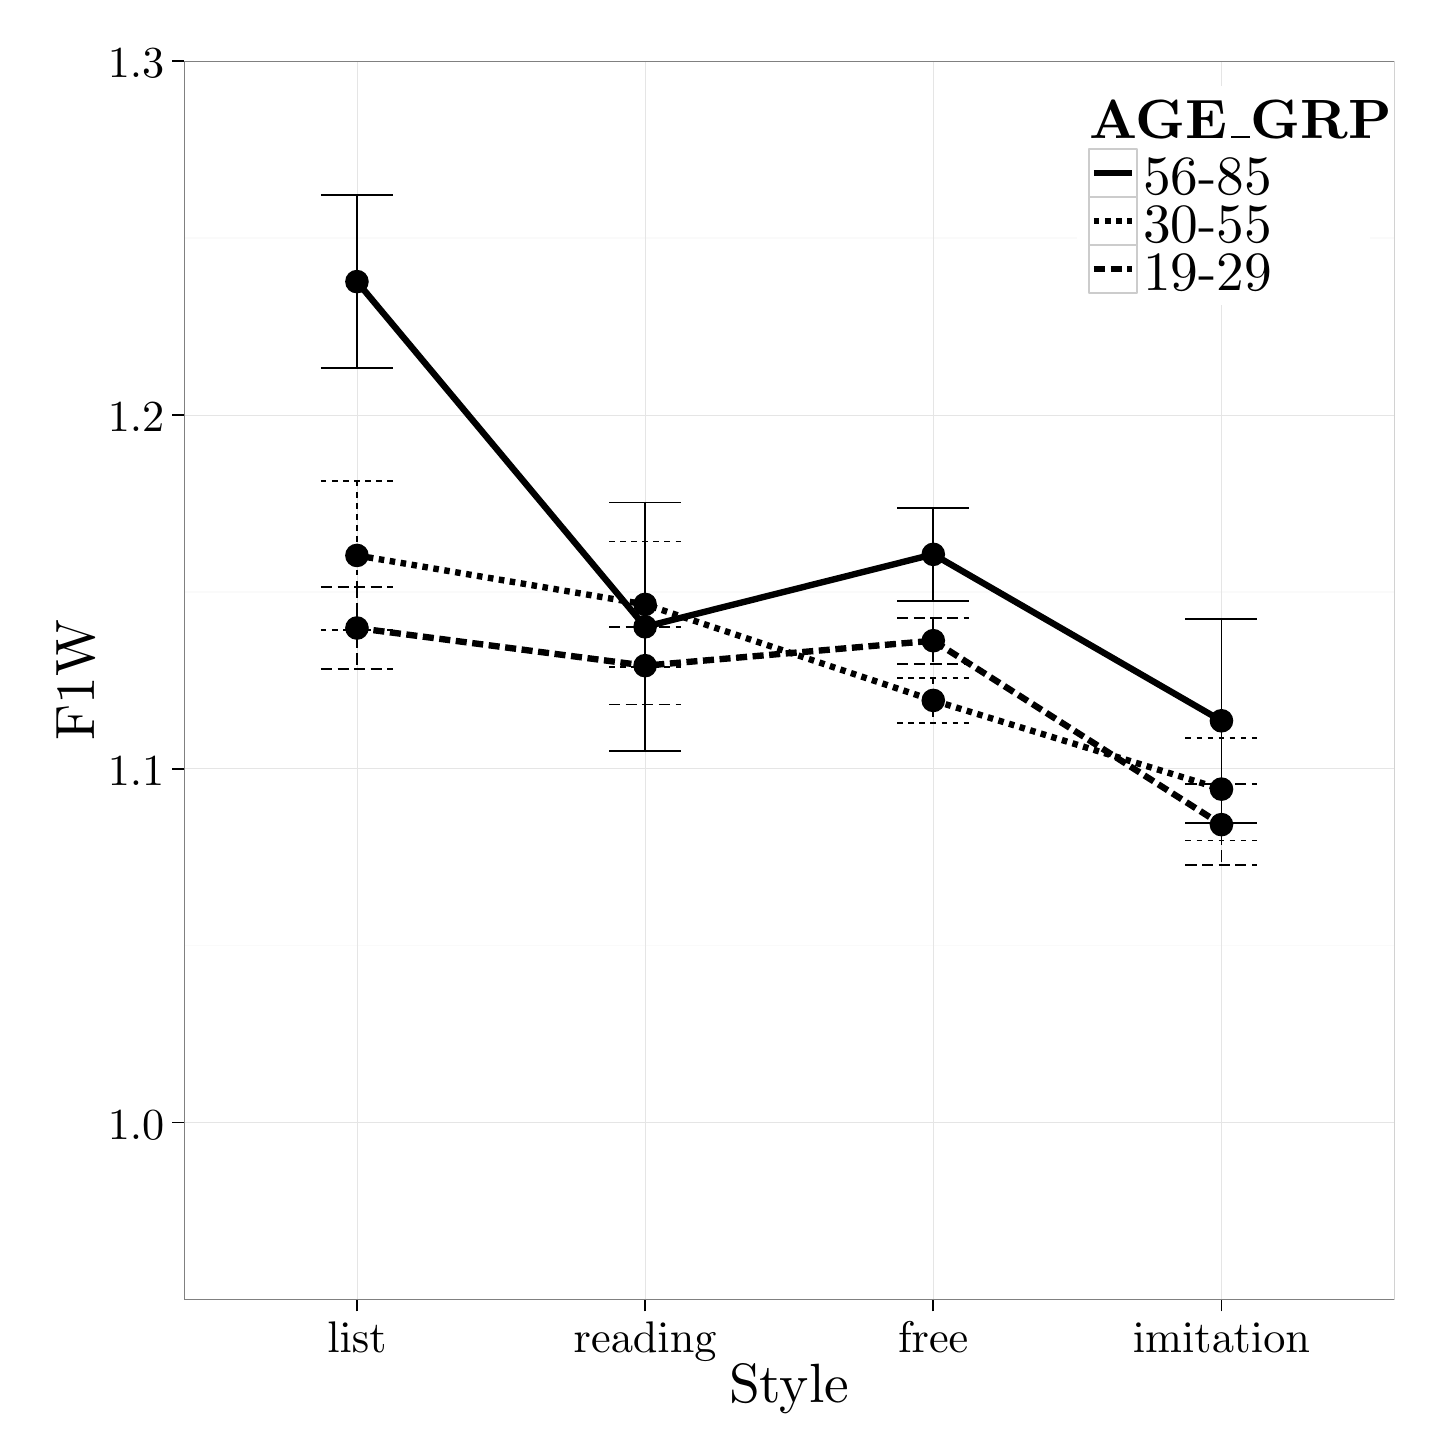
\begin{tikzpicture}[x=1pt,y=1pt]
\definecolor{fillColor}{RGB}{255,255,255}
\path[use as bounding box,fill=fillColor,fill opacity=0.00] (0,0) rectangle (505.89,505.89);
\begin{scope}
\path[clip] (  0.00,  0.00) rectangle (505.89,505.89);
\definecolor{drawColor}{RGB}{255,255,255}
\definecolor{fillColor}{RGB}{255,255,255}

\path[draw=drawColor,line width= 0.6pt,line join=round,line cap=round,fill=fillColor] (  0.00, -0.00) rectangle (505.89,505.89);
\end{scope}
\begin{scope}
\path[clip] ( 56.50, 46.31) rectangle (493.85,493.84);
\definecolor{fillColor}{RGB}{255,255,255}

\path[fill=fillColor] ( 56.50, 46.31) rectangle (493.85,493.84);
\definecolor{drawColor}{gray}{0.98}

\path[draw=drawColor,line width= 0.6pt,line join=round] ( 56.50, 46.31) --
	(493.85, 46.31);

\path[draw=drawColor,line width= 0.6pt,line join=round] ( 56.50,174.18) --
	(493.85,174.18);

\path[draw=drawColor,line width= 0.6pt,line join=round] ( 56.50,302.04) --
	(493.85,302.04);

\path[draw=drawColor,line width= 0.6pt,line join=round] ( 56.50,429.91) --
	(493.85,429.91);
\definecolor{drawColor}{gray}{0.90}

\path[draw=drawColor,line width= 0.2pt,line join=round] ( 56.50,110.24) --
	(493.85,110.24);

\path[draw=drawColor,line width= 0.2pt,line join=round] ( 56.50,238.11) --
	(493.85,238.11);

\path[draw=drawColor,line width= 0.2pt,line join=round] ( 56.50,365.98) --
	(493.85,365.98);

\path[draw=drawColor,line width= 0.2pt,line join=round] ( 56.50,493.84) --
	(493.85,493.84);

\path[draw=drawColor,line width= 0.2pt,line join=round] (118.98, 46.31) --
	(118.98,493.84);

\path[draw=drawColor,line width= 0.2pt,line join=round] (223.11, 46.31) --
	(223.11,493.84);

\path[draw=drawColor,line width= 0.2pt,line join=round] (327.24, 46.31) --
	(327.24,493.84);

\path[draw=drawColor,line width= 0.2pt,line join=round] (431.37, 46.31) --
	(431.37,493.84);
\definecolor{fillColor}{RGB}{0,0,0}

\path[fill=fillColor] (118.98,414.12) circle (  4.27);

\path[fill=fillColor] (118.98,315.18) circle (  4.27);

\path[fill=fillColor] (118.98,288.95) circle (  4.27);

\path[fill=fillColor] (223.11,289.40) circle (  4.27);

\path[fill=fillColor] (223.11,297.48) circle (  4.27);

\path[fill=fillColor] (223.11,275.35) circle (  4.27);

\path[fill=fillColor] (327.24,315.57) circle (  4.27);

\path[fill=fillColor] (327.24,262.78) circle (  4.27);

\path[fill=fillColor] (327.24,284.37) circle (  4.27);

\path[fill=fillColor] (431.37,255.43) circle (  4.27);

\path[fill=fillColor] (431.37,230.74) circle (  4.27);

\path[fill=fillColor] (431.37,217.91) circle (  4.27);
\definecolor{drawColor}{RGB}{0,0,0}

\path[draw=drawColor,line width= 2.3pt,line join=round] (118.98,414.12) --
	(223.11,289.40) --
	(327.24,315.57) --
	(431.37,255.43);

\path[draw=drawColor,line width= 2.3pt,dash pattern=on 2pt off 2pt ,line join=round] (118.98,315.18) --
	(223.11,297.48) --
	(327.24,262.78) --
	(431.37,230.74);

\path[draw=drawColor,line width= 2.3pt,dash pattern=on 4pt off 2pt ,line join=round] (118.98,288.95) --
	(223.11,275.35) --
	(327.24,284.37) --
	(431.37,217.91);

\path[draw=drawColor,line width= 0.6pt,line join=round] (105.96,445.35) --
	(132.00,445.35);

\path[draw=drawColor,line width= 0.6pt,line join=round] (118.98,445.35) --
	(118.98,382.89);

\path[draw=drawColor,line width= 0.6pt,line join=round] (105.96,382.89) --
	(132.00,382.89);

\path[draw=drawColor,line width= 0.6pt,line join=round] (210.09,334.29) --
	(236.13,334.29);

\path[draw=drawColor,line width= 0.6pt,line join=round] (223.11,334.29) --
	(223.11,244.52);

\path[draw=drawColor,line width= 0.6pt,line join=round] (210.09,244.52) --
	(236.13,244.52);

\path[draw=drawColor,line width= 0.6pt,line join=round] (314.22,332.33) --
	(340.25,332.33);

\path[draw=drawColor,line width= 0.6pt,line join=round] (327.24,332.33) --
	(327.24,298.80);

\path[draw=drawColor,line width= 0.6pt,line join=round] (314.22,298.80) --
	(340.25,298.80);

\path[draw=drawColor,line width= 0.6pt,line join=round] (418.35,292.28) --
	(444.38,292.28);

\path[draw=drawColor,line width= 0.6pt,line join=round] (431.37,292.28) --
	(431.37,218.59);

\path[draw=drawColor,line width= 0.6pt,line join=round] (418.35,218.59) --
	(444.38,218.59);

\path[draw=drawColor,line width= 0.6pt,dash pattern=on 2pt off 2pt ,line join=round] (105.96,342.09) --
	(132.00,342.09);

\path[draw=drawColor,line width= 0.6pt,dash pattern=on 2pt off 2pt ,line join=round] (118.98,342.09) --
	(118.98,288.27);

\path[draw=drawColor,line width= 0.6pt,dash pattern=on 2pt off 2pt ,line join=round] (105.96,288.27) --
	(132.00,288.27);

\path[draw=drawColor,line width= 0.6pt,dash pattern=on 2pt off 2pt ,line join=round] (210.09,320.22) --
	(236.13,320.22);

\path[draw=drawColor,line width= 0.6pt,dash pattern=on 2pt off 2pt ,line join=round] (223.11,320.22) --
	(223.11,274.75);

\path[draw=drawColor,line width= 0.6pt,dash pattern=on 2pt off 2pt ,line join=round] (210.09,274.75) --
	(236.13,274.75);

\path[draw=drawColor,line width= 0.6pt,dash pattern=on 2pt off 2pt ,line join=round] (314.22,270.87) --
	(340.25,270.87);

\path[draw=drawColor,line width= 0.6pt,dash pattern=on 2pt off 2pt ,line join=round] (327.24,270.87) --
	(327.24,254.70);

\path[draw=drawColor,line width= 0.6pt,dash pattern=on 2pt off 2pt ,line join=round] (314.22,254.70) --
	(340.25,254.70);

\path[draw=drawColor,line width= 0.6pt,dash pattern=on 2pt off 2pt ,line join=round] (418.35,249.32) --
	(444.38,249.32);

\path[draw=drawColor,line width= 0.6pt,dash pattern=on 2pt off 2pt ,line join=round] (431.37,249.32) --
	(431.37,212.16);

\path[draw=drawColor,line width= 0.6pt,dash pattern=on 2pt off 2pt ,line join=round] (418.35,212.16) --
	(444.38,212.16);

\path[draw=drawColor,line width= 0.6pt,dash pattern=on 4pt off 2pt ,line join=round] (105.96,303.75) --
	(132.00,303.75);

\path[draw=drawColor,line width= 0.6pt,dash pattern=on 4pt off 2pt ,line join=round] (118.98,303.75) --
	(118.98,274.16);

\path[draw=drawColor,line width= 0.6pt,dash pattern=on 4pt off 2pt ,line join=round] (105.96,274.16) --
	(132.00,274.16);

\path[draw=drawColor,line width= 0.6pt,dash pattern=on 4pt off 2pt ,line join=round] (210.09,289.34) --
	(236.13,289.34);

\path[draw=drawColor,line width= 0.6pt,dash pattern=on 4pt off 2pt ,line join=round] (223.11,289.34) --
	(223.11,261.36);

\path[draw=drawColor,line width= 0.6pt,dash pattern=on 4pt off 2pt ,line join=round] (210.09,261.36) --
	(236.13,261.36);

\path[draw=drawColor,line width= 0.6pt,dash pattern=on 4pt off 2pt ,line join=round] (314.22,292.69) --
	(340.25,292.69);

\path[draw=drawColor,line width= 0.6pt,dash pattern=on 4pt off 2pt ,line join=round] (327.24,292.69) --
	(327.24,276.06);

\path[draw=drawColor,line width= 0.6pt,dash pattern=on 4pt off 2pt ,line join=round] (314.22,276.06) --
	(340.25,276.06);

\path[draw=drawColor,line width= 0.6pt,dash pattern=on 4pt off 2pt ,line join=round] (418.35,232.57) --
	(444.38,232.57);

\path[draw=drawColor,line width= 0.6pt,dash pattern=on 4pt off 2pt ,line join=round] (431.37,232.57) --
	(431.37,203.26);

\path[draw=drawColor,line width= 0.6pt,dash pattern=on 4pt off 2pt ,line join=round] (418.35,203.26) --
	(444.38,203.26);
\definecolor{drawColor}{gray}{0.50}

\path[draw=drawColor,line width= 0.6pt,line join=round,line cap=round] ( 56.50, 46.31) rectangle (493.85,493.84);
\end{scope}
\begin{scope}
\path[clip] (  0.00,  0.00) rectangle (505.89,505.89);
\definecolor{drawColor}{RGB}{0,0,0}

\node[text=drawColor,anchor=base east,inner sep=0pt, outer sep=0pt, scale=  1.60] at ( 49.39,104.21) {1.0};

\node[text=drawColor,anchor=base east,inner sep=0pt, outer sep=0pt, scale=  1.60] at ( 49.39,232.08) {1.1};

\node[text=drawColor,anchor=base east,inner sep=0pt, outer sep=0pt, scale=  1.60] at ( 49.39,359.94) {1.2};

\node[text=drawColor,anchor=base east,inner sep=0pt, outer sep=0pt, scale=  1.60] at ( 49.39,487.81) {1.3};
\end{scope}
\begin{scope}
\path[clip] (  0.00,  0.00) rectangle (505.89,505.89);
\definecolor{drawColor}{RGB}{0,0,0}

\path[draw=drawColor,line width= 0.6pt,line join=round] ( 52.24,110.24) --
	( 56.50,110.24);

\path[draw=drawColor,line width= 0.6pt,line join=round] ( 52.24,238.11) --
	( 56.50,238.11);

\path[draw=drawColor,line width= 0.6pt,line join=round] ( 52.24,365.98) --
	( 56.50,365.98);

\path[draw=drawColor,line width= 0.6pt,line join=round] ( 52.24,493.84) --
	( 56.50,493.84);
\end{scope}
\begin{scope}
\path[clip] (  0.00,  0.00) rectangle (505.89,505.89);
\definecolor{drawColor}{RGB}{0,0,0}

\path[draw=drawColor,line width= 0.6pt,line join=round] (118.98, 42.04) --
	(118.98, 46.31);

\path[draw=drawColor,line width= 0.6pt,line join=round] (223.11, 42.04) --
	(223.11, 46.31);

\path[draw=drawColor,line width= 0.6pt,line join=round] (327.24, 42.04) --
	(327.24, 46.31);

\path[draw=drawColor,line width= 0.6pt,line join=round] (431.37, 42.04) --
	(431.37, 46.31);
\end{scope}
\begin{scope}
\path[clip] (  0.00,  0.00) rectangle (505.89,505.89);
\definecolor{drawColor}{RGB}{0,0,0}

\node[text=drawColor,anchor=base,inner sep=0pt, outer sep=0pt, scale=  1.60] at (118.98, 27.13) {list};

\node[text=drawColor,anchor=base,inner sep=0pt, outer sep=0pt, scale=  1.60] at (223.11, 27.13) {reading};

\node[text=drawColor,anchor=base,inner sep=0pt, outer sep=0pt, scale=  1.60] at (327.24, 27.13) {free};

\node[text=drawColor,anchor=base,inner sep=0pt, outer sep=0pt, scale=  1.60] at (431.37, 27.13) {imitation};
\end{scope}
\begin{scope}
\path[clip] (  0.00,  0.00) rectangle (505.89,505.89);
\definecolor{drawColor}{RGB}{0,0,0}

\node[text=drawColor,anchor=base,inner sep=0pt, outer sep=0pt, scale=  2.00] at (275.17,  9.03) {Style};
\end{scope}
\begin{scope}
\path[clip] (  0.00,  0.00) rectangle (505.89,505.89);
\definecolor{drawColor}{RGB}{0,0,0}

\node[text=drawColor,rotate= 90.00,anchor=base,inner sep=0pt, outer sep=0pt, scale=  2.00] at ( 24.12,270.08) {F1W};
\end{scope}
\begin{scope}
\path[clip] (  0.00,  0.00) rectangle (505.89,505.89);
\definecolor{fillColor}{RGB}{255,255,255}

\path[fill=fillColor] (379.28,405.66) rectangle (484.98,484.98);
\end{scope}
\begin{scope}
\path[clip] (  0.00,  0.00) rectangle (505.89,505.89);
\definecolor{drawColor}{RGB}{0,0,0}

\node[text=drawColor,anchor=base west,inner sep=0pt, outer sep=0pt, scale=  2.00] at (383.55,465.96) {\bfseries AGE{\_{}}GRP};
\end{scope}
\begin{scope}
\path[clip] (  0.00,  0.00) rectangle (505.89,505.89);
\definecolor{drawColor}{gray}{0.80}
\definecolor{fillColor}{RGB}{255,255,255}

\path[draw=drawColor,line width= 0.6pt,line join=round,line cap=round,fill=fillColor] (383.55,444.61) rectangle (400.89,461.96);
\end{scope}
\begin{scope}
\path[clip] (  0.00,  0.00) rectangle (505.89,505.89);
\definecolor{drawColor}{RGB}{0,0,0}

\path[draw=drawColor,line width= 2.3pt,line join=round] (385.28,453.29) -- (399.16,453.29);
\end{scope}
\begin{scope}
\path[clip] (  0.00,  0.00) rectangle (505.89,505.89);
\definecolor{drawColor}{RGB}{0,0,0}

\path[draw=drawColor,line width= 0.6pt,line join=round] (385.28,453.29) -- (399.16,453.29);
\end{scope}
\begin{scope}
\path[clip] (  0.00,  0.00) rectangle (505.89,505.89);
\definecolor{drawColor}{gray}{0.80}
\definecolor{fillColor}{RGB}{255,255,255}

\path[draw=drawColor,line width= 0.6pt,line join=round,line cap=round,fill=fillColor] (383.55,427.27) rectangle (400.89,444.61);
\end{scope}
\begin{scope}
\path[clip] (  0.00,  0.00) rectangle (505.89,505.89);
\definecolor{drawColor}{RGB}{0,0,0}

\path[draw=drawColor,line width= 2.3pt,dash pattern=on 2pt off 2pt ,line join=round] (385.28,435.94) -- (399.16,435.94);
\end{scope}
\begin{scope}
\path[clip] (  0.00,  0.00) rectangle (505.89,505.89);
\definecolor{drawColor}{RGB}{0,0,0}

\path[draw=drawColor,line width= 0.6pt,dash pattern=on 2pt off 2pt ,line join=round] (385.28,435.94) -- (399.16,435.94);
\end{scope}
\begin{scope}
\path[clip] (  0.00,  0.00) rectangle (505.89,505.89);
\definecolor{drawColor}{gray}{0.80}
\definecolor{fillColor}{RGB}{255,255,255}

\path[draw=drawColor,line width= 0.6pt,line join=round,line cap=round,fill=fillColor] (383.55,409.92) rectangle (400.89,427.27);
\end{scope}
\begin{scope}
\path[clip] (  0.00,  0.00) rectangle (505.89,505.89);
\definecolor{drawColor}{RGB}{0,0,0}

\path[draw=drawColor,line width= 2.3pt,dash pattern=on 4pt off 2pt ,line join=round] (385.28,418.60) -- (399.16,418.60);
\end{scope}
\begin{scope}
\path[clip] (  0.00,  0.00) rectangle (505.89,505.89);
\definecolor{drawColor}{RGB}{0,0,0}

\path[draw=drawColor,line width= 0.6pt,dash pattern=on 4pt off 2pt ,line join=round] (385.28,418.60) -- (399.16,418.60);
\end{scope}
\begin{scope}
\path[clip] (  0.00,  0.00) rectangle (505.89,505.89);
\definecolor{drawColor}{RGB}{0,0,0}

\node[text=drawColor,anchor=base west,inner sep=0pt, outer sep=0pt, scale=  2.00] at (403.06,445.75) {56-85};
\end{scope}
\begin{scope}
\path[clip] (  0.00,  0.00) rectangle (505.89,505.89);
\definecolor{drawColor}{RGB}{0,0,0}

\node[text=drawColor,anchor=base west,inner sep=0pt, outer sep=0pt, scale=  2.00] at (403.06,428.40) {30-55};
\end{scope}
\begin{scope}
\path[clip] (  0.00,  0.00) rectangle (505.89,505.89);
\definecolor{drawColor}{RGB}{0,0,0}

\node[text=drawColor,anchor=base west,inner sep=0pt, outer sep=0pt, scale=  2.00] at (403.06,411.06) {19-29};
\end{scope}
\end{tikzpicture}
} 
		\caption{middle class}
		\label{fig.line.f1.nurse.mc}
	\end{subfigure}
	\begin{subfigure}{.49\textwidth}
		\centering
			\definecolor{shadecolor}{rgb}{0.969, 0.969, 0.969}
			\resizebox{\linewidth}{!}{% Created by tikzDevice version 0.8.1 on 2016-02-09 02:14:49
% !TEX encoding = UTF-8 Unicode
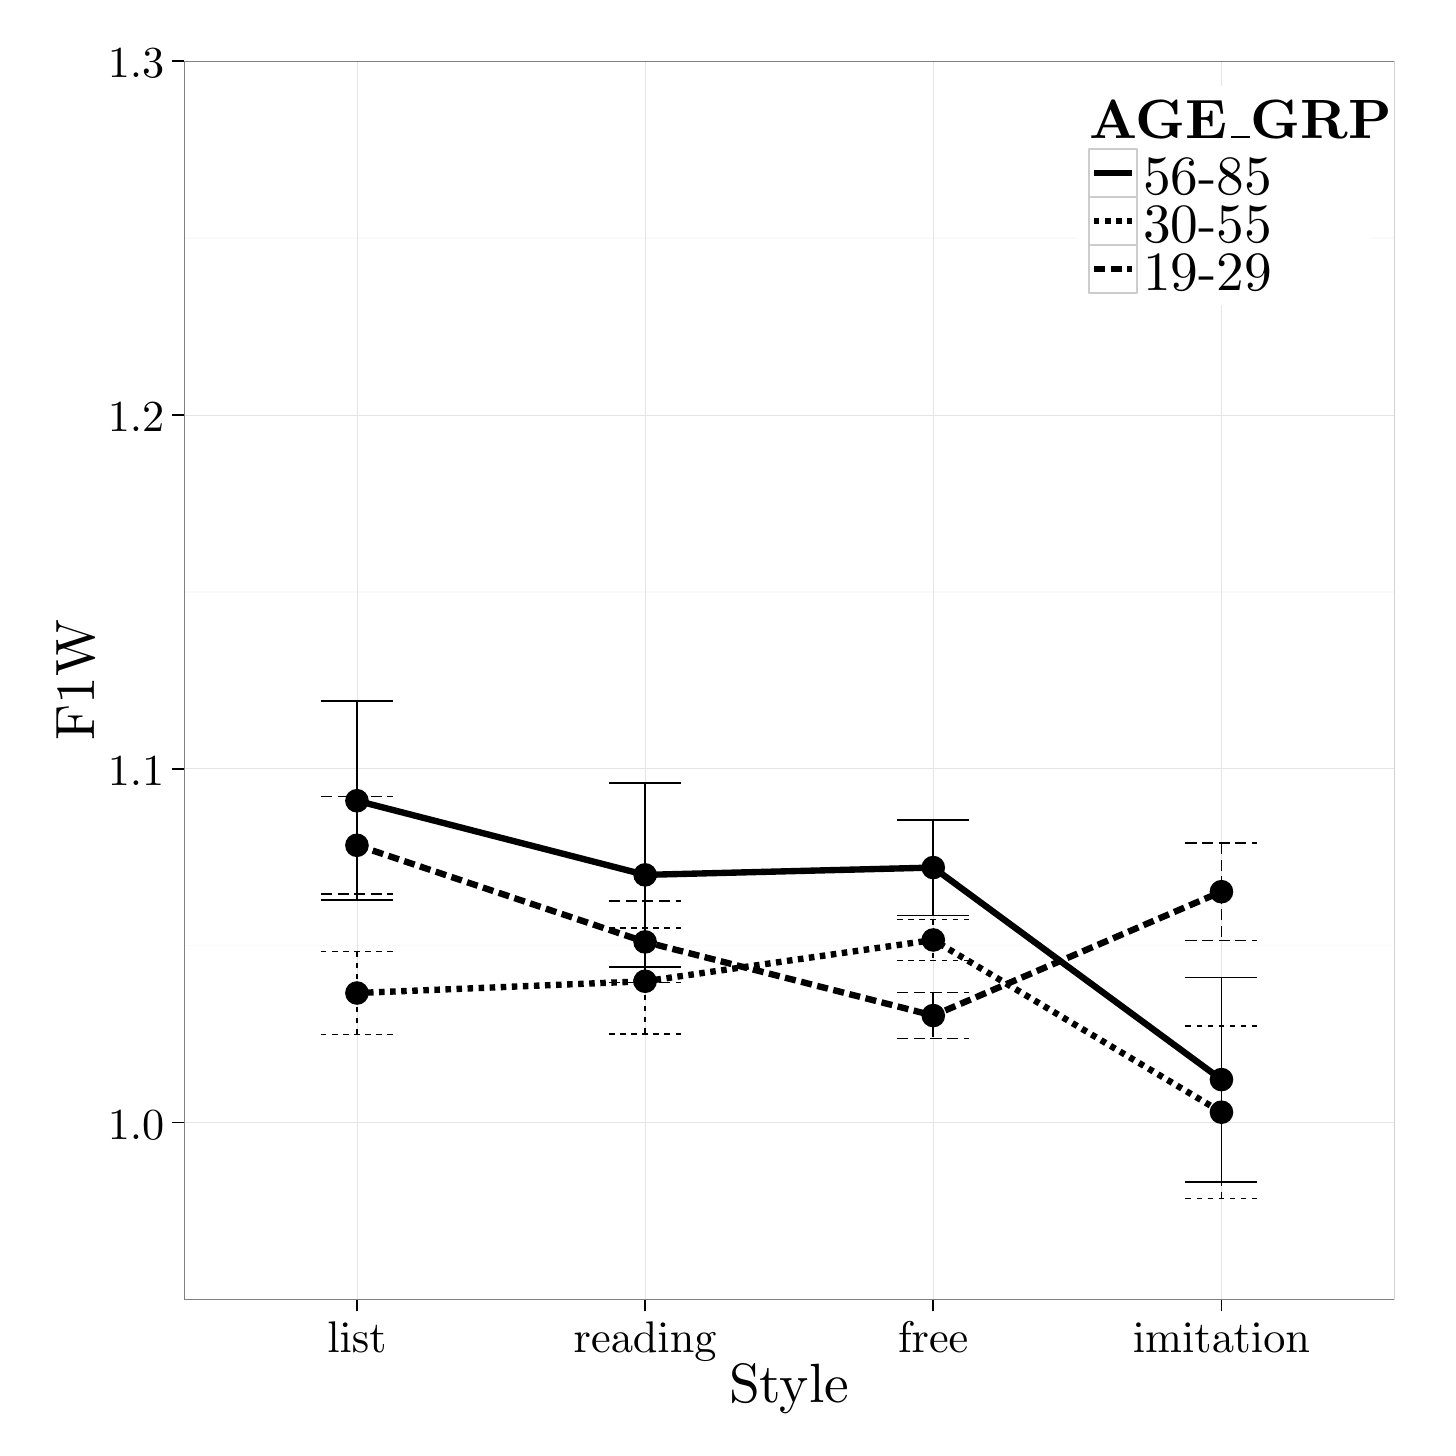
\begin{tikzpicture}[x=1pt,y=1pt]
\definecolor{fillColor}{RGB}{255,255,255}
\path[use as bounding box,fill=fillColor,fill opacity=0.00] (0,0) rectangle (505.89,505.89);
\begin{scope}
\path[clip] (  0.00,  0.00) rectangle (505.89,505.89);
\definecolor{drawColor}{RGB}{255,255,255}
\definecolor{fillColor}{RGB}{255,255,255}

\path[draw=drawColor,line width= 0.6pt,line join=round,line cap=round,fill=fillColor] (  0.00, -0.00) rectangle (505.89,505.89);
\end{scope}
\begin{scope}
\path[clip] ( 56.50, 46.31) rectangle (493.85,493.84);
\definecolor{fillColor}{RGB}{255,255,255}

\path[fill=fillColor] ( 56.50, 46.31) rectangle (493.85,493.84);
\definecolor{drawColor}{gray}{0.98}

\path[draw=drawColor,line width= 0.6pt,line join=round] ( 56.50, 46.31) --
	(493.85, 46.31);

\path[draw=drawColor,line width= 0.6pt,line join=round] ( 56.50,174.18) --
	(493.85,174.18);

\path[draw=drawColor,line width= 0.6pt,line join=round] ( 56.50,302.04) --
	(493.85,302.04);

\path[draw=drawColor,line width= 0.6pt,line join=round] ( 56.50,429.91) --
	(493.85,429.91);
\definecolor{drawColor}{gray}{0.90}

\path[draw=drawColor,line width= 0.2pt,line join=round] ( 56.50,110.24) --
	(493.85,110.24);

\path[draw=drawColor,line width= 0.2pt,line join=round] ( 56.50,238.11) --
	(493.85,238.11);

\path[draw=drawColor,line width= 0.2pt,line join=round] ( 56.50,365.98) --
	(493.85,365.98);

\path[draw=drawColor,line width= 0.2pt,line join=round] ( 56.50,493.84) --
	(493.85,493.84);

\path[draw=drawColor,line width= 0.2pt,line join=round] (118.98, 46.31) --
	(118.98,493.84);

\path[draw=drawColor,line width= 0.2pt,line join=round] (223.11, 46.31) --
	(223.11,493.84);

\path[draw=drawColor,line width= 0.2pt,line join=round] (327.24, 46.31) --
	(327.24,493.84);

\path[draw=drawColor,line width= 0.2pt,line join=round] (431.37, 46.31) --
	(431.37,493.84);
\definecolor{fillColor}{RGB}{0,0,0}

\path[fill=fillColor] (118.98,226.54) circle (  4.27);

\path[fill=fillColor] (118.98,157.06) circle (  4.27);

\path[fill=fillColor] (118.98,210.44) circle (  4.27);

\path[fill=fillColor] (223.11,199.75) circle (  4.27);

\path[fill=fillColor] (223.11,161.31) circle (  4.27);

\path[fill=fillColor] (223.11,175.53) circle (  4.27);

\path[fill=fillColor] (327.24,202.39) circle (  4.27);

\path[fill=fillColor] (327.24,176.23) circle (  4.27);

\path[fill=fillColor] (327.24,148.91) circle (  4.27);

\path[fill=fillColor] (431.37,125.78) circle (  4.27);

\path[fill=fillColor] (431.37,113.99) circle (  4.27);

\path[fill=fillColor] (431.37,193.67) circle (  4.27);
\definecolor{drawColor}{RGB}{0,0,0}

\path[draw=drawColor,line width= 2.3pt,line join=round] (118.98,226.54) --
	(223.11,199.75) --
	(327.24,202.39) --
	(431.37,125.78);

\path[draw=drawColor,line width= 2.3pt,dash pattern=on 2pt off 2pt ,line join=round] (118.98,157.06) --
	(223.11,161.31) --
	(327.24,176.23) --
	(431.37,113.99);

\path[draw=drawColor,line width= 2.3pt,dash pattern=on 4pt off 2pt ,line join=round] (118.98,210.44) --
	(223.11,175.53) --
	(327.24,148.91) --
	(431.37,193.67);

\path[draw=drawColor,line width= 0.6pt,line join=round] (105.96,262.50) --
	(132.00,262.50);

\path[draw=drawColor,line width= 0.6pt,line join=round] (118.98,262.50) --
	(118.98,190.58);

\path[draw=drawColor,line width= 0.6pt,line join=round] (105.96,190.58) --
	(132.00,190.58);

\path[draw=drawColor,line width= 0.6pt,line join=round] (210.09,232.95) --
	(236.13,232.95);

\path[draw=drawColor,line width= 0.6pt,line join=round] (223.11,232.95) --
	(223.11,166.55);

\path[draw=drawColor,line width= 0.6pt,line join=round] (210.09,166.55) --
	(236.13,166.55);

\path[draw=drawColor,line width= 0.6pt,line join=round] (314.22,219.66) --
	(340.25,219.66);

\path[draw=drawColor,line width= 0.6pt,line join=round] (327.24,219.66) --
	(327.24,185.12);

\path[draw=drawColor,line width= 0.6pt,line join=round] (314.22,185.12) --
	(340.25,185.12);

\path[draw=drawColor,line width= 0.6pt,line join=round] (418.35,162.70) --
	(444.38,162.70);

\path[draw=drawColor,line width= 0.6pt,line join=round] (431.37,162.70) --
	(431.37, 88.86);

\path[draw=drawColor,line width= 0.6pt,line join=round] (418.35, 88.86) --
	(444.38, 88.86);

\path[draw=drawColor,line width= 0.6pt,dash pattern=on 2pt off 2pt ,line join=round] (105.96,172.08) --
	(132.00,172.08);

\path[draw=drawColor,line width= 0.6pt,dash pattern=on 2pt off 2pt ,line join=round] (118.98,172.08) --
	(118.98,142.03);

\path[draw=drawColor,line width= 0.6pt,dash pattern=on 2pt off 2pt ,line join=round] (105.96,142.03) --
	(132.00,142.03);

\path[draw=drawColor,line width= 0.6pt,dash pattern=on 2pt off 2pt ,line join=round] (210.09,180.47) --
	(236.13,180.47);

\path[draw=drawColor,line width= 0.6pt,dash pattern=on 2pt off 2pt ,line join=round] (223.11,180.47) --
	(223.11,142.16);

\path[draw=drawColor,line width= 0.6pt,dash pattern=on 2pt off 2pt ,line join=round] (210.09,142.16) --
	(236.13,142.16);

\path[draw=drawColor,line width= 0.6pt,dash pattern=on 2pt off 2pt ,line join=round] (314.22,183.61) --
	(340.25,183.61);

\path[draw=drawColor,line width= 0.6pt,dash pattern=on 2pt off 2pt ,line join=round] (327.24,183.61) --
	(327.24,168.85);

\path[draw=drawColor,line width= 0.6pt,dash pattern=on 2pt off 2pt ,line join=round] (314.22,168.85) --
	(340.25,168.85);

\path[draw=drawColor,line width= 0.6pt,dash pattern=on 2pt off 2pt ,line join=round] (418.35,145.16) --
	(444.38,145.16);

\path[draw=drawColor,line width= 0.6pt,dash pattern=on 2pt off 2pt ,line join=round] (431.37,145.16) --
	(431.37, 82.83);

\path[draw=drawColor,line width= 0.6pt,dash pattern=on 2pt off 2pt ,line join=round] (418.35, 82.83) --
	(444.38, 82.83);

\path[draw=drawColor,line width= 0.6pt,dash pattern=on 4pt off 2pt ,line join=round] (105.96,228.12) --
	(132.00,228.12);

\path[draw=drawColor,line width= 0.6pt,dash pattern=on 4pt off 2pt ,line join=round] (118.98,228.12) --
	(118.98,192.76);

\path[draw=drawColor,line width= 0.6pt,dash pattern=on 4pt off 2pt ,line join=round] (105.96,192.76) --
	(132.00,192.76);

\path[draw=drawColor,line width= 0.6pt,dash pattern=on 4pt off 2pt ,line join=round] (210.09,190.22) --
	(236.13,190.22);

\path[draw=drawColor,line width= 0.6pt,dash pattern=on 4pt off 2pt ,line join=round] (223.11,190.22) --
	(223.11,160.84);

\path[draw=drawColor,line width= 0.6pt,dash pattern=on 4pt off 2pt ,line join=round] (210.09,160.84) --
	(236.13,160.84);

\path[draw=drawColor,line width= 0.6pt,dash pattern=on 4pt off 2pt ,line join=round] (314.22,157.26) --
	(340.25,157.26);

\path[draw=drawColor,line width= 0.6pt,dash pattern=on 4pt off 2pt ,line join=round] (327.24,157.26) --
	(327.24,140.57);

\path[draw=drawColor,line width= 0.6pt,dash pattern=on 4pt off 2pt ,line join=round] (314.22,140.57) --
	(340.25,140.57);

\path[draw=drawColor,line width= 0.6pt,dash pattern=on 4pt off 2pt ,line join=round] (418.35,211.30) --
	(444.38,211.30);

\path[draw=drawColor,line width= 0.6pt,dash pattern=on 4pt off 2pt ,line join=round] (431.37,211.30) --
	(431.37,176.03);

\path[draw=drawColor,line width= 0.6pt,dash pattern=on 4pt off 2pt ,line join=round] (418.35,176.03) --
	(444.38,176.03);
\definecolor{drawColor}{gray}{0.50}

\path[draw=drawColor,line width= 0.6pt,line join=round,line cap=round] ( 56.50, 46.31) rectangle (493.85,493.84);
\end{scope}
\begin{scope}
\path[clip] (  0.00,  0.00) rectangle (505.89,505.89);
\definecolor{drawColor}{RGB}{0,0,0}

\node[text=drawColor,anchor=base east,inner sep=0pt, outer sep=0pt, scale=  1.60] at ( 49.39,104.21) {1.0};

\node[text=drawColor,anchor=base east,inner sep=0pt, outer sep=0pt, scale=  1.60] at ( 49.39,232.08) {1.1};

\node[text=drawColor,anchor=base east,inner sep=0pt, outer sep=0pt, scale=  1.60] at ( 49.39,359.94) {1.2};

\node[text=drawColor,anchor=base east,inner sep=0pt, outer sep=0pt, scale=  1.60] at ( 49.39,487.81) {1.3};
\end{scope}
\begin{scope}
\path[clip] (  0.00,  0.00) rectangle (505.89,505.89);
\definecolor{drawColor}{RGB}{0,0,0}

\path[draw=drawColor,line width= 0.6pt,line join=round] ( 52.24,110.24) --
	( 56.50,110.24);

\path[draw=drawColor,line width= 0.6pt,line join=round] ( 52.24,238.11) --
	( 56.50,238.11);

\path[draw=drawColor,line width= 0.6pt,line join=round] ( 52.24,365.98) --
	( 56.50,365.98);

\path[draw=drawColor,line width= 0.6pt,line join=round] ( 52.24,493.84) --
	( 56.50,493.84);
\end{scope}
\begin{scope}
\path[clip] (  0.00,  0.00) rectangle (505.89,505.89);
\definecolor{drawColor}{RGB}{0,0,0}

\path[draw=drawColor,line width= 0.6pt,line join=round] (118.98, 42.04) --
	(118.98, 46.31);

\path[draw=drawColor,line width= 0.6pt,line join=round] (223.11, 42.04) --
	(223.11, 46.31);

\path[draw=drawColor,line width= 0.6pt,line join=round] (327.24, 42.04) --
	(327.24, 46.31);

\path[draw=drawColor,line width= 0.6pt,line join=round] (431.37, 42.04) --
	(431.37, 46.31);
\end{scope}
\begin{scope}
\path[clip] (  0.00,  0.00) rectangle (505.89,505.89);
\definecolor{drawColor}{RGB}{0,0,0}

\node[text=drawColor,anchor=base,inner sep=0pt, outer sep=0pt, scale=  1.60] at (118.98, 27.13) {list};

\node[text=drawColor,anchor=base,inner sep=0pt, outer sep=0pt, scale=  1.60] at (223.11, 27.13) {reading};

\node[text=drawColor,anchor=base,inner sep=0pt, outer sep=0pt, scale=  1.60] at (327.24, 27.13) {free};

\node[text=drawColor,anchor=base,inner sep=0pt, outer sep=0pt, scale=  1.60] at (431.37, 27.13) {imitation};
\end{scope}
\begin{scope}
\path[clip] (  0.00,  0.00) rectangle (505.89,505.89);
\definecolor{drawColor}{RGB}{0,0,0}

\node[text=drawColor,anchor=base,inner sep=0pt, outer sep=0pt, scale=  2.00] at (275.17,  9.03) {Style};
\end{scope}
\begin{scope}
\path[clip] (  0.00,  0.00) rectangle (505.89,505.89);
\definecolor{drawColor}{RGB}{0,0,0}

\node[text=drawColor,rotate= 90.00,anchor=base,inner sep=0pt, outer sep=0pt, scale=  2.00] at ( 24.12,270.08) {F1W};
\end{scope}
\begin{scope}
\path[clip] (  0.00,  0.00) rectangle (505.89,505.89);
\definecolor{fillColor}{RGB}{255,255,255}

\path[fill=fillColor] (379.28,405.66) rectangle (484.98,484.98);
\end{scope}
\begin{scope}
\path[clip] (  0.00,  0.00) rectangle (505.89,505.89);
\definecolor{drawColor}{RGB}{0,0,0}

\node[text=drawColor,anchor=base west,inner sep=0pt, outer sep=0pt, scale=  2.00] at (383.55,465.96) {\bfseries AGE{\_{}}GRP};
\end{scope}
\begin{scope}
\path[clip] (  0.00,  0.00) rectangle (505.89,505.89);
\definecolor{drawColor}{gray}{0.80}
\definecolor{fillColor}{RGB}{255,255,255}

\path[draw=drawColor,line width= 0.6pt,line join=round,line cap=round,fill=fillColor] (383.55,444.61) rectangle (400.89,461.96);
\end{scope}
\begin{scope}
\path[clip] (  0.00,  0.00) rectangle (505.89,505.89);
\definecolor{drawColor}{RGB}{0,0,0}

\path[draw=drawColor,line width= 2.3pt,line join=round] (385.28,453.29) -- (399.16,453.29);
\end{scope}
\begin{scope}
\path[clip] (  0.00,  0.00) rectangle (505.89,505.89);
\definecolor{drawColor}{RGB}{0,0,0}

\path[draw=drawColor,line width= 0.6pt,line join=round] (385.28,453.29) -- (399.16,453.29);
\end{scope}
\begin{scope}
\path[clip] (  0.00,  0.00) rectangle (505.89,505.89);
\definecolor{drawColor}{gray}{0.80}
\definecolor{fillColor}{RGB}{255,255,255}

\path[draw=drawColor,line width= 0.6pt,line join=round,line cap=round,fill=fillColor] (383.55,427.27) rectangle (400.89,444.61);
\end{scope}
\begin{scope}
\path[clip] (  0.00,  0.00) rectangle (505.89,505.89);
\definecolor{drawColor}{RGB}{0,0,0}

\path[draw=drawColor,line width= 2.3pt,dash pattern=on 2pt off 2pt ,line join=round] (385.28,435.94) -- (399.16,435.94);
\end{scope}
\begin{scope}
\path[clip] (  0.00,  0.00) rectangle (505.89,505.89);
\definecolor{drawColor}{RGB}{0,0,0}

\path[draw=drawColor,line width= 0.6pt,dash pattern=on 2pt off 2pt ,line join=round] (385.28,435.94) -- (399.16,435.94);
\end{scope}
\begin{scope}
\path[clip] (  0.00,  0.00) rectangle (505.89,505.89);
\definecolor{drawColor}{gray}{0.80}
\definecolor{fillColor}{RGB}{255,255,255}

\path[draw=drawColor,line width= 0.6pt,line join=round,line cap=round,fill=fillColor] (383.55,409.92) rectangle (400.89,427.27);
\end{scope}
\begin{scope}
\path[clip] (  0.00,  0.00) rectangle (505.89,505.89);
\definecolor{drawColor}{RGB}{0,0,0}

\path[draw=drawColor,line width= 2.3pt,dash pattern=on 4pt off 2pt ,line join=round] (385.28,418.60) -- (399.16,418.60);
\end{scope}
\begin{scope}
\path[clip] (  0.00,  0.00) rectangle (505.89,505.89);
\definecolor{drawColor}{RGB}{0,0,0}

\path[draw=drawColor,line width= 0.6pt,dash pattern=on 4pt off 2pt ,line join=round] (385.28,418.60) -- (399.16,418.60);
\end{scope}
\begin{scope}
\path[clip] (  0.00,  0.00) rectangle (505.89,505.89);
\definecolor{drawColor}{RGB}{0,0,0}

\node[text=drawColor,anchor=base west,inner sep=0pt, outer sep=0pt, scale=  2.00] at (403.06,445.75) {56-85};
\end{scope}
\begin{scope}
\path[clip] (  0.00,  0.00) rectangle (505.89,505.89);
\definecolor{drawColor}{RGB}{0,0,0}

\node[text=drawColor,anchor=base west,inner sep=0pt, outer sep=0pt, scale=  2.00] at (403.06,428.40) {30-55};
\end{scope}
\begin{scope}
\path[clip] (  0.00,  0.00) rectangle (505.89,505.89);
\definecolor{drawColor}{RGB}{0,0,0}

\node[text=drawColor,anchor=base west,inner sep=0pt, outer sep=0pt, scale=  2.00] at (403.06,411.06) {19-29};
\end{scope}
\end{tikzpicture}
} 
		\caption{working class}
		\label{fig.line.f1.nurse.wc}
	\end{subfigure}
	\caption{\textsc{nurse} (F1) by style, age, and social class}
\end{figure}

The interaction of style, age, and social class presents itself as somewhat more messy.
Speakers in the old group can be said to be the ones where social class seems to play the least important role with respect to \isi{style shifting}.
In both the middle (Figure \ref{fig.line.f1.nurse.mc}) and the working class (Figure \ref{fig.line.f1.nurse.wc}), the general tendency for F1 values to decrease from most formal to least formal context is visible.
Admittedly, vowels elicited by the word list are only (significantly) more open for old middle-class speakers, but, on the other hand, in \emph{both} classes
\begin{inparaenum}[(a)]
	\item realisations in the `reading' and `free' registers are not significantly different from each other, and
	\item F1 of \textsc{nurse} is (just about) significantly lower in accent perform\is{accent performance}ance (`imitation\is{accent performance}') than in spontaneous speech (`free').
\end{inparaenum}

Middle-aged subjects in the middle-class sub-sample generate the neatest version of the downward trend that should by now be familiar.
First of all, F1 values for the dotted line decrease linearly, without exception, from left to right in Figure \ref{fig.line.f1.nurse.wc}.
Second, if we lump together the word list and the reading passage (which do not seem to be different in a statistically robust way), this decrease is also significant from `reading'/`word list' to `free', and from `free' to `imitation\is{accent performance}'.
Working-class speakers of the same age group do not show this regular downward trend.
What is more, \textsc{nurse} realisations in the registers word list, reading passage, and spontaneous speech are not --- statistically speaking --- different.
When perform\is{accent performance}ing Scouse, variants are significantly higher, but only when compared to free speech; the overlapping error whiskers in Figure \ref{fig.line.f1.nurse.wc} indicate that `list', `reading', and `imitation\is{accent performance}' are not significantly different for subjects aged between 30 and 55.

For the youngest group of speakers it is in the \emph{middle} class where these three styles are not significantly different from one another.
Accent perform\is{accent performance}ance, however, is then (highly) significantly different from all other registers.
Young working-class speakers echo middle-aged middle-class participants in that they have a linear decrease in F1 from `list' to `free'.
In addition, both `list' and 'reading' \emph{and} `reading' and `free' are (at least marginally) significantly different.
As a sort of reversal of the pattern found for middle-aged working-class speakers, there is then an increase towards the values found for `imitation\is{accent performance}', a mean which is again only significantly different from spontaneous speech, but not the reading passage or the word list.
There is thus a general similarity between Figures \ref{fig.line.f1.nurse.women} and \ref{fig.line.f1.nurse.mc} (downward trend more visible) and \ref{fig.line.f1.nurse.wc} and \ref{fig.line.f1.nurse.men} (flatter lines), which is in line with an immense body of sociolinguistic research that has, time and again, found female speakers and those of higher socioeconomic classes to be more sensitive to sociolinguistically meaningful variables.
If we zoom in, however, it becomes obvious that the middle-aged group exhibits a more linear pattern in the middle class (as expected), whereas the youngest speakers actually have a flatter line in this class than in the working class.

\subsection{F2 (\textsc{nurse})}
\label{sec.prod.res.vow.nurse.f2}

\subsubsection{Overview}
\label{sec.prod.res.vow.nurse.f2.overview}

Compared to the model reported for F1 measurements of \textsc{nurse}, the mixed linear effects regression of F2 obviously has a different dependent variable, but since there was an F2 measurement for every corresponding observation of F1, the independent variables (and their distribution within the dataset) are the same.
Collinearity\is{collinearity} was therefore reduced in exactly the same way that was described at the beginning of Section \ref{sec.prod.res.vow.nurse.f1}.
Model selection based on AIC scores and F-tests comparing nested models resulted in the minimal adequate model shown below (Table \ref{tab.regression.nurse.f2}, R\textsuperscript{2}-equivalent = 0.66).

{
	\footnotesize
	\begin{longtable}[c]{p{0.3\textwidth}rrrrrl}
		\caption{\textsc{nurse} (F2): mixed linear effects regression}\label{tab.regression.nurse.f2}\\
				
		\hline
		Fixed effects: & Estimate & Std. Error & df & t value & Pr($>$$|$t$|$) & \\ 
		\hline
		(Intercept) & 1.40 & 0.01 & 347.52 & 103.21 & < 0.001 & *** \\ 
		STYLElist & -0.01 & 0.01 & 1514.59 & -1.33 & 0.18 & \\ 
		STYLEread & -0.03 & 0.01 & 1533.43 & -5.22 & < 0.001 & *** \\ 
		STYLEfree & 0.01 & 0.01 & 870.58 & 1.20 & 0.23 & \\ 
		AGE56-85 & -0.03 & 0.01 & 1432.62 & -5.14 & < 0.001 & *** \\ 
		AGE30-55 & 0.00 & 0.00 & 1447.88 & 0.38 & 0.70 & \\ 
		GENDERf & 0.05 & 0.00 & 1516.12 & 18.82 & < 0.001 & *** \\ 
		CLASSmc & -0.06 & 0.00 & 1444.81 & -18.59 & < 0.001 & *** \\ 
		DURATION & 0.00 & 0.00 & 1506.54 & 3.16 & < 0.01 & ** \\ 
		PREMANNERaffr & 0.07 & 0.02 & 71.47 & 3.44 & < 0.001 & *** \\ 
		PREMANNERfric & 0.00 & 0.01 & 86.50 & 0.41 & 0.68 & \\ 
		PREMANNERgli & -0.07 & 0.01 & 62.72 & -4.53 & < 0.001 & *** \\ 
		PREMANNERliq & -0.03 & 0.03 & 91.59 & -1.07 & 0.29 & \\ 
		PREMANNERnas & 0.01 & 0.02 & 159.94 & 0.57 & 0.57 & \\ 
		STYLElist:AGE56-85 & -0.05 & 0.01 & 1425.23 & -4.97 & < 0.001 & *** \\ 
		STYLEread:AGE56-85 & -0.01 & 0.01 & 1419.97 & -1.33 & 0.18 & \\ 
		STYLEfree:AGE56-85 & -0.02 & 0.01 & 1493.50 & -3.29 & < 0.01 & ** \\ 
		STYLElist:AGE30-55 & 0.02 & 0.01 & 1426.13 & 2.37 & 0.02 & * \\ 
		STYLEread:AGE30-55 & 0.02 & 0.01 & 1430.56 & 2.05 & 0.04 & * \\ 
		STYLEfree:AGE30-55 & 0.01 & 0.01 & 1493.35 & 2.63 & 0.01 & **\\ 
		STYLElist:CLASSmc & -0.02 & 0.01 & 1424.03 & -3.49 & < 0.001 & *** \\ 
		STYLEread:CLASSmc & 0.01 & 0.01 & 1425.34 & 0.99 & 0.32 & \\ 
		STYLEfree:CLASSmc & -0.01 & 0.00 & 1495.02 & -2.31 & 0.02 & *\\ 
		AGE56-85:GENDERf & -0.02 & 0.00 & 1518.78 & -5.49 & < 0.001 & *** \\ 
		AGE30-55:GENDERf & 0.07 & 0.00 & 1512.01 & 22.03 & < 0.001 & *** \\ 
		AGE56-85:CLASSmc & -0.05 & 0.01 & 1431.94 & -10.02 & < 0.001 & *** \\ 
		AGE30-55:CLASSmc & 0.02 & 0.00 & 1449.85 & 4.97 & < 0.001 & *** \\ 
		GENDERf:CLASSmc & -0.02 & 0.00 & 1517.33 & -8.76 & < 0.001 & *** \\ 
		STYLElist:AGE56-85:CLASSmc & 0.04 & 0.01 & 1426.89 & 4.02 & < 0.001 & *** \\ 
		STYLEread:AGE56-85:CLASSmc & 0.00 & 0.01 & 1419.93 & 0.52 & 0.61 & \\ 
		STYLEfree:AGE56-85:CLASSmc & -0.00 & 0.01 & 1481.98 & -0.41 & 0.68 & \\ 
		STYLElist:AGE30-55:CLASSmc & -0.02 & 0.01 & 1427.41 & -2.22 & 0.03 & * \\ 
		STYLEread:AGE30-55:CLASSmc & -0.01 & 0.01 & 1430.06 & -1.78 & 0.08 & .\\ 
		STYLEfree:AGE30-55:CLASSmc & -0.01 & 0.01 & 1487.18 & -1.03 & 0.30 & \\ 
		\hline
		Random effects: & \multicolumn{6}{l}{(number of obs: 1568, groups: WORD, 137)} \\
		Groups &         Name & Variance &      Std.Dev. & & & \\
		WORD &  (Intercept) & 0.002 & 0.044 & & & \\
		Residual  &         & 0.008 & 0.091 & & & \\
		\hline
	\end{longtable}
	
}


This model contains all the social factors as significant fixed effects which were already found to be signifiant predictors when modelling the F1 values of \textsc{nurse}.
The only exception to this is the three-way interaction of style, age, and gender which does not reach statistical significance in the regression of F2.
Age, gender, and social class of participant, however, are all significant main effects.
So is speaking style, which further acts as a predictor of F2 in two-way interactions with age and social class.
Gender of speaker also interacts with social class and age each.
Age, finally, furthermore appears both in a significant two-way interaction with social class and a three-way interaction of style, age group, and social class.
In addition to the social categories, phonetic and phonological predictors are more important than they were for the height dimension of \textsc{nurse}: both the preceding consonant and the duration of the observed vowel have a significant impact on F2 values of \textsc{nurse}.
It is these two factors which we will look at first.

\subsubsection{Phonological context}
\label{sec.prod.res.vow.nurse.f2.phon}

\begin{figure}[h!]
	\centering
		\definecolor{shadecolor}{rgb}{0.969, 0.969, 0.969}
		\resizebox{0.5\linewidth}{!}{% Created by tikzDevice version 0.8.1 on 2016-02-09 02:14:52
% !TEX encoding = UTF-8 Unicode
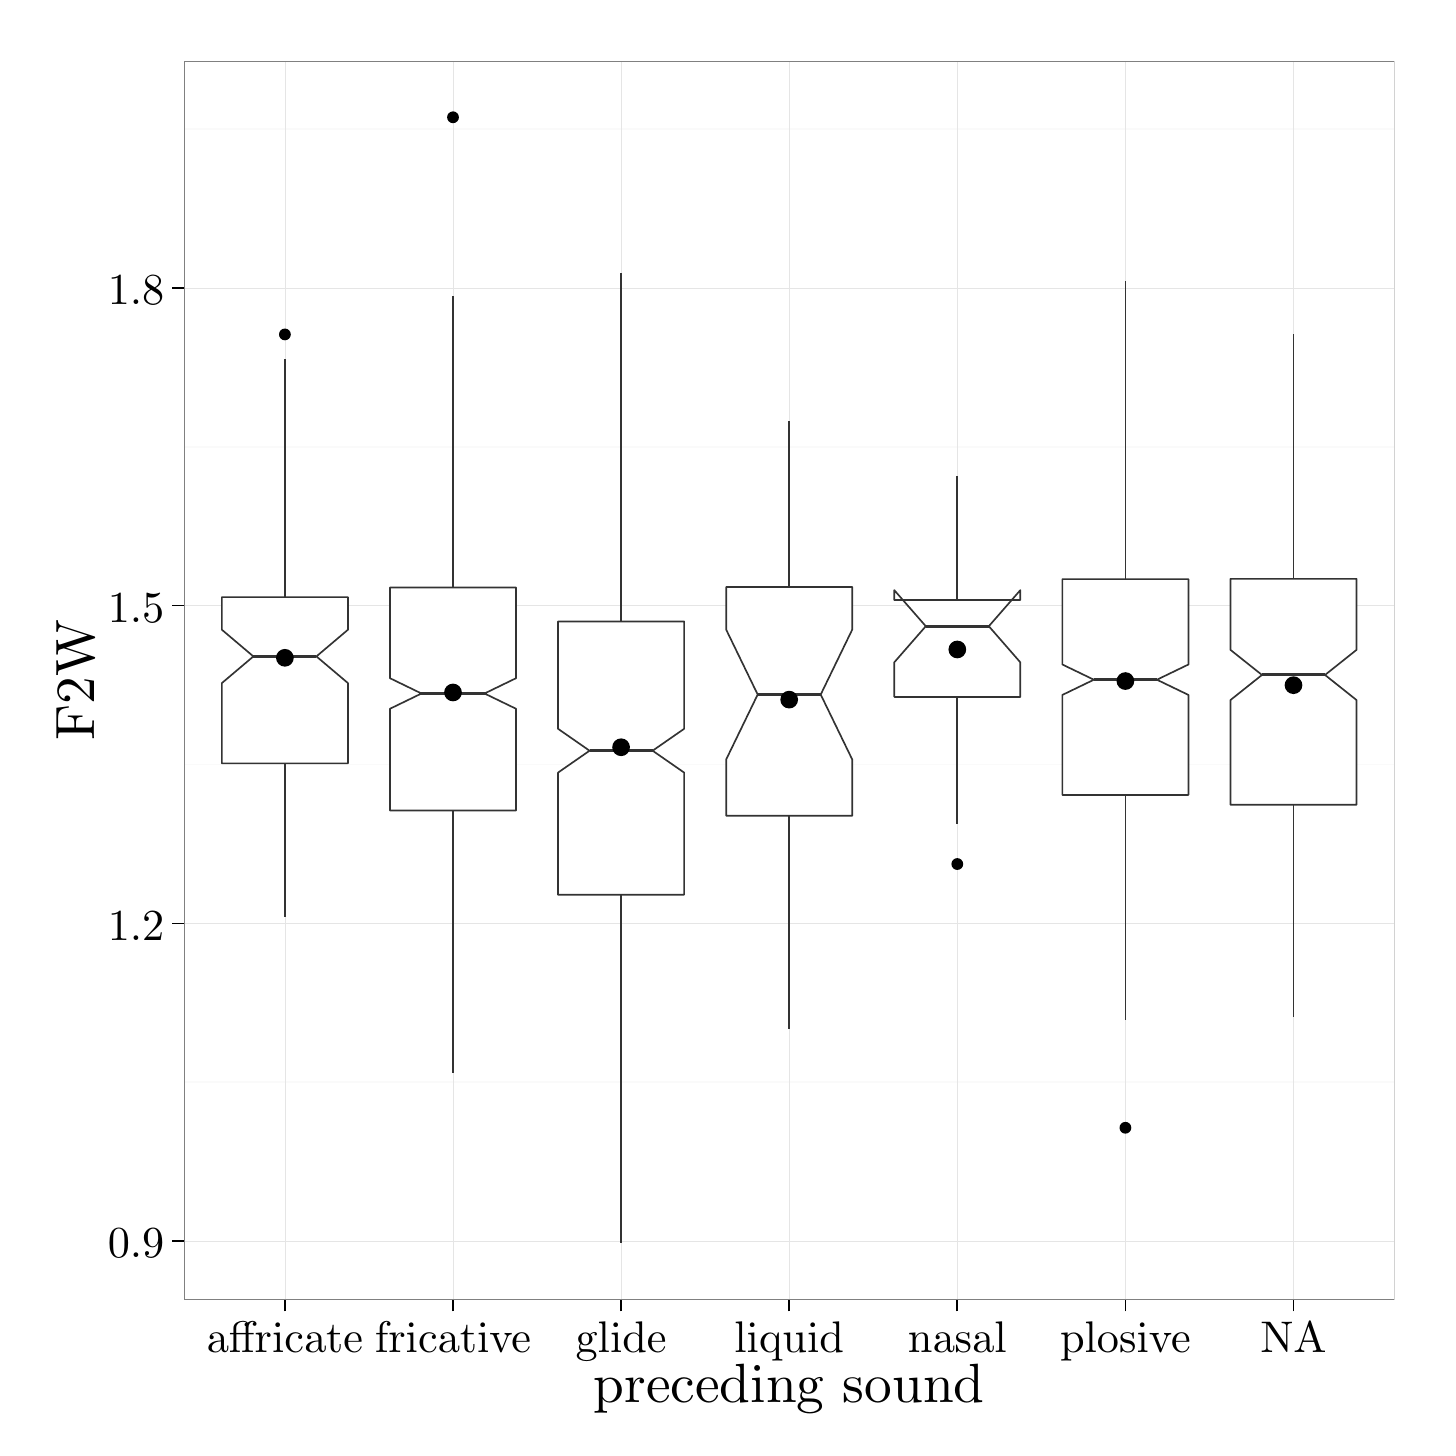
\begin{tikzpicture}[x=1pt,y=1pt]
\definecolor{fillColor}{RGB}{255,255,255}
\path[use as bounding box,fill=fillColor,fill opacity=0.00] (0,0) rectangle (505.89,505.89);
\begin{scope}
\path[clip] (  0.00,  0.00) rectangle (505.89,505.89);
\definecolor{drawColor}{RGB}{255,255,255}
\definecolor{fillColor}{RGB}{255,255,255}

\path[draw=drawColor,line width= 0.6pt,line join=round,line cap=round,fill=fillColor] (  0.00, -0.00) rectangle (505.89,505.89);
\end{scope}
\begin{scope}
\path[clip] ( 56.50, 46.31) rectangle (493.85,493.84);
\definecolor{fillColor}{RGB}{255,255,255}

\path[fill=fillColor] ( 56.50, 46.31) rectangle (493.85,493.84);
\definecolor{drawColor}{gray}{0.98}

\path[draw=drawColor,line width= 0.6pt,line join=round] ( 56.50,124.83) --
	(493.85,124.83);

\path[draw=drawColor,line width= 0.6pt,line join=round] ( 56.50,239.65) --
	(493.85,239.65);

\path[draw=drawColor,line width= 0.6pt,line join=round] ( 56.50,354.47) --
	(493.85,354.47);

\path[draw=drawColor,line width= 0.6pt,line join=round] ( 56.50,469.29) --
	(493.85,469.29);
\definecolor{drawColor}{gray}{0.90}

\path[draw=drawColor,line width= 0.2pt,line join=round] ( 56.50, 67.42) --
	(493.85, 67.42);

\path[draw=drawColor,line width= 0.2pt,line join=round] ( 56.50,182.24) --
	(493.85,182.24);

\path[draw=drawColor,line width= 0.2pt,line join=round] ( 56.50,297.06) --
	(493.85,297.06);

\path[draw=drawColor,line width= 0.2pt,line join=round] ( 56.50,411.88) --
	(493.85,411.88);

\path[draw=drawColor,line width= 0.2pt,line join=round] ( 92.95, 46.31) --
	( 92.95,493.84);

\path[draw=drawColor,line width= 0.2pt,line join=round] (153.69, 46.31) --
	(153.69,493.84);

\path[draw=drawColor,line width= 0.2pt,line join=round] (214.43, 46.31) --
	(214.43,493.84);

\path[draw=drawColor,line width= 0.2pt,line join=round] (275.17, 46.31) --
	(275.17,493.84);

\path[draw=drawColor,line width= 0.2pt,line join=round] (335.92, 46.31) --
	(335.92,493.84);

\path[draw=drawColor,line width= 0.2pt,line join=round] (396.66, 46.31) --
	(396.66,493.84);

\path[draw=drawColor,line width= 0.2pt,line join=round] (457.40, 46.31) --
	(457.40,493.84);
\definecolor{fillColor}{RGB}{0,0,0}

\path[fill=fillColor] ( 92.95,395.04) circle (  2.13);
\definecolor{drawColor}{gray}{0.20}

\path[draw=drawColor,line width= 0.6pt,line join=round] ( 92.95,300.12) -- ( 92.95,386.24);

\path[draw=drawColor,line width= 0.6pt,line join=round] ( 92.95,240.03) -- ( 92.95,184.53);
\definecolor{fillColor}{RGB}{255,255,255}

\path[draw=drawColor,line width= 0.6pt,line join=round,line cap=round,fill=fillColor] ( 70.17,300.12) --
	( 70.17,288.33) --
	( 81.56,278.69) --
	( 70.17,269.05) --
	( 70.17,240.03) --
	(115.73,240.03) --
	(115.73,269.05) --
	(104.34,278.69) --
	(115.73,288.33) --
	(115.73,300.12) --
	( 70.17,300.12) --
	cycle;

\path[draw=drawColor,line width= 1.1pt,line join=round] ( 81.56,278.69) -- (104.34,278.69);
\definecolor{fillColor}{RGB}{0,0,0}

\path[fill=fillColor] (153.69,473.50) circle (  2.13);

\path[draw=drawColor,line width= 0.6pt,line join=round] (153.69,303.57) -- (153.69,408.82);

\path[draw=drawColor,line width= 0.6pt,line join=round] (153.69,223.00) -- (153.69,128.27);
\definecolor{fillColor}{RGB}{255,255,255}

\path[draw=drawColor,line width= 0.6pt,line join=round,line cap=round,fill=fillColor] (130.91,303.57) --
	(130.91,270.82) --
	(142.30,265.29) --
	(130.91,259.77) --
	(130.91,223.00) --
	(176.47,223.00) --
	(176.47,259.77) --
	(165.08,265.29) --
	(176.47,270.82) --
	(176.47,303.57) --
	(130.91,303.57) --
	cycle;

\path[draw=drawColor,line width= 1.1pt,line join=round] (142.30,265.29) -- (165.08,265.29);

\path[draw=drawColor,line width= 0.6pt,line join=round] (214.43,291.32) -- (214.43,417.24);

\path[draw=drawColor,line width= 0.6pt,line join=round] (214.43,192.57) -- (214.43, 66.65);

\path[draw=drawColor,line width= 0.6pt,line join=round,line cap=round,fill=fillColor] (191.65,291.32) --
	(191.65,252.53) --
	(203.04,244.62) --
	(191.65,236.71) --
	(191.65,192.57) --
	(237.21,192.57) --
	(237.21,236.71) --
	(225.82,244.62) --
	(237.21,252.53) --
	(237.21,291.32) --
	(191.65,291.32) --
	cycle;

\path[draw=drawColor,line width= 1.1pt,line join=round] (203.04,244.62) -- (225.82,244.62);

\path[draw=drawColor,line width= 0.6pt,line join=round] (275.17,303.76) -- (275.17,363.66);

\path[draw=drawColor,line width= 0.6pt,line join=round] (275.17,221.09) -- (275.17,143.96);

\path[draw=drawColor,line width= 0.6pt,line join=round,line cap=round,fill=fillColor] (252.40,303.76) --
	(252.40,288.37) --
	(263.79,264.91) --
	(252.40,241.45) --
	(252.40,221.09) --
	(297.95,221.09) --
	(297.95,241.45) --
	(286.56,264.91) --
	(297.95,288.37) --
	(297.95,303.76) --
	(252.40,303.76) --
	cycle;

\path[draw=drawColor,line width= 1.1pt,line join=round] (263.79,264.91) -- (286.56,264.91);
\definecolor{fillColor}{RGB}{0,0,0}

\path[fill=fillColor] (335.92,203.67) circle (  2.13);

\path[draw=drawColor,line width= 0.6pt,line join=round] (335.92,299.07) -- (335.92,343.75);

\path[draw=drawColor,line width= 0.6pt,line join=round] (335.92,264.05) -- (335.92,218.22);
\definecolor{fillColor}{RGB}{255,255,255}

\path[draw=drawColor,line width= 0.6pt,line join=round,line cap=round,fill=fillColor] (313.14,299.07) --
	(313.14,302.64) --
	(324.53,289.60) --
	(313.14,276.55) --
	(313.14,264.05) --
	(358.69,264.05) --
	(358.69,276.55) --
	(347.31,289.60) --
	(358.69,302.64) --
	(358.69,299.07) --
	(313.14,299.07) --
	cycle;

\path[draw=drawColor,line width= 1.1pt,line join=round] (324.53,289.60) -- (347.31,289.60);
\definecolor{fillColor}{RGB}{0,0,0}

\path[fill=fillColor] (396.66,108.37) circle (  2.13);

\path[draw=drawColor,line width= 0.6pt,line join=round] (396.66,306.63) -- (396.66,414.18);

\path[draw=drawColor,line width= 0.6pt,line join=round] (396.66,228.64) -- (396.66,147.41);
\definecolor{fillColor}{RGB}{255,255,255}

\path[draw=drawColor,line width= 0.6pt,line join=round,line cap=round,fill=fillColor] (373.88,306.63) --
	(373.88,275.77) --
	(385.27,270.27) --
	(373.88,264.77) --
	(373.88,228.64) --
	(419.44,228.64) --
	(419.44,264.77) --
	(408.05,270.27) --
	(419.44,275.77) --
	(419.44,306.63) --
	(373.88,306.63) --
	cycle;

\path[draw=drawColor,line width= 1.1pt,line join=round] (385.27,270.27) -- (408.05,270.27);

\path[draw=drawColor,line width= 0.6pt,line join=round] (457.40,306.72) -- (457.40,395.04);

\path[draw=drawColor,line width= 0.6pt,line join=round] (457.40,225.10) -- (457.40,148.56);

\path[draw=drawColor,line width= 0.6pt,line join=round,line cap=round,fill=fillColor] (434.62,306.72) --
	(434.62,281.06) --
	(446.01,271.99) --
	(434.62,262.92) --
	(434.62,225.10) --
	(480.18,225.10) --
	(480.18,262.92) --
	(468.79,271.99) --
	(480.18,281.06) --
	(480.18,306.72) --
	(434.62,306.72) --
	cycle;

\path[draw=drawColor,line width= 1.1pt,line join=round] (446.01,271.99) -- (468.79,271.99);
\definecolor{fillColor}{RGB}{0,0,0}

\path[fill=fillColor] ( 92.95,278.19) circle (  3.20);

\path[fill=fillColor] (153.69,265.66) circle (  3.20);

\path[fill=fillColor] (214.43,245.87) circle (  3.20);

\path[fill=fillColor] (275.17,263.08) circle (  3.20);

\path[fill=fillColor] (335.92,281.20) circle (  3.20);

\path[fill=fillColor] (396.66,269.79) circle (  3.20);

\path[fill=fillColor] (457.40,268.29) circle (  3.20);
\definecolor{drawColor}{gray}{0.50}

\path[draw=drawColor,line width= 0.6pt,line join=round,line cap=round] ( 56.50, 46.31) rectangle (493.85,493.84);
\end{scope}
\begin{scope}
\path[clip] (  0.00,  0.00) rectangle (505.89,505.89);
\definecolor{drawColor}{RGB}{0,0,0}

\node[text=drawColor,anchor=base east,inner sep=0pt, outer sep=0pt, scale=  1.60] at ( 49.39, 61.38) {0.9};

\node[text=drawColor,anchor=base east,inner sep=0pt, outer sep=0pt, scale=  1.60] at ( 49.39,176.20) {1.2};

\node[text=drawColor,anchor=base east,inner sep=0pt, outer sep=0pt, scale=  1.60] at ( 49.39,291.03) {1.5};

\node[text=drawColor,anchor=base east,inner sep=0pt, outer sep=0pt, scale=  1.60] at ( 49.39,405.85) {1.8};
\end{scope}
\begin{scope}
\path[clip] (  0.00,  0.00) rectangle (505.89,505.89);
\definecolor{drawColor}{RGB}{0,0,0}

\path[draw=drawColor,line width= 0.6pt,line join=round] ( 52.24, 67.42) --
	( 56.50, 67.42);

\path[draw=drawColor,line width= 0.6pt,line join=round] ( 52.24,182.24) --
	( 56.50,182.24);

\path[draw=drawColor,line width= 0.6pt,line join=round] ( 52.24,297.06) --
	( 56.50,297.06);

\path[draw=drawColor,line width= 0.6pt,line join=round] ( 52.24,411.88) --
	( 56.50,411.88);
\end{scope}
\begin{scope}
\path[clip] (  0.00,  0.00) rectangle (505.89,505.89);
\definecolor{drawColor}{RGB}{0,0,0}

\path[draw=drawColor,line width= 0.6pt,line join=round] ( 92.95, 42.04) --
	( 92.95, 46.31);

\path[draw=drawColor,line width= 0.6pt,line join=round] (153.69, 42.04) --
	(153.69, 46.31);

\path[draw=drawColor,line width= 0.6pt,line join=round] (214.43, 42.04) --
	(214.43, 46.31);

\path[draw=drawColor,line width= 0.6pt,line join=round] (275.17, 42.04) --
	(275.17, 46.31);

\path[draw=drawColor,line width= 0.6pt,line join=round] (335.92, 42.04) --
	(335.92, 46.31);

\path[draw=drawColor,line width= 0.6pt,line join=round] (396.66, 42.04) --
	(396.66, 46.31);

\path[draw=drawColor,line width= 0.6pt,line join=round] (457.40, 42.04) --
	(457.40, 46.31);
\end{scope}
\begin{scope}
\path[clip] (  0.00,  0.00) rectangle (505.89,505.89);
\definecolor{drawColor}{RGB}{0,0,0}

\node[text=drawColor,anchor=base,inner sep=0pt, outer sep=0pt, scale=  1.60] at ( 92.95, 27.13) {affricate};

\node[text=drawColor,anchor=base,inner sep=0pt, outer sep=0pt, scale=  1.60] at (153.69, 27.13) {fricative};

\node[text=drawColor,anchor=base,inner sep=0pt, outer sep=0pt, scale=  1.60] at (214.43, 27.13) {glide};

\node[text=drawColor,anchor=base,inner sep=0pt, outer sep=0pt, scale=  1.60] at (275.17, 27.13) {liquid};

\node[text=drawColor,anchor=base,inner sep=0pt, outer sep=0pt, scale=  1.60] at (335.92, 27.13) {nasal};

\node[text=drawColor,anchor=base,inner sep=0pt, outer sep=0pt, scale=  1.60] at (396.66, 27.13) {plosive};

\node[text=drawColor,anchor=base,inner sep=0pt, outer sep=0pt, scale=  1.60] at (457.40, 27.13) {NA};
\end{scope}
\begin{scope}
\path[clip] (  0.00,  0.00) rectangle (505.89,505.89);
\definecolor{drawColor}{RGB}{0,0,0}

\node[text=drawColor,anchor=base,inner sep=0pt, outer sep=0pt, scale=  2.00] at (275.17,  9.03) {preceding sound};
\end{scope}
\begin{scope}
\path[clip] (  0.00,  0.00) rectangle (505.89,505.89);
\definecolor{drawColor}{RGB}{0,0,0}

\node[text=drawColor,rotate= 90.00,anchor=base,inner sep=0pt, outer sep=0pt, scale=  2.00] at ( 24.12,270.08) {F2W};
\end{scope}
\end{tikzpicture}
} 
	\caption{\textsc{nurse} (F2) by preceding sound}
	\label{fig.box.f2w.nurse.presound}
\end{figure}

The mixed linear effects regression found two levels of the factor (manner of) preceding consonant in particular to have a significant impact on F2 of \textsc{nurse}.
A positive correlation coefficient was calculated for cases where \textsc{nurse} is preceded by an affricate (indicating that this \isi{phonological context} favours fronter, more Scouse, realisations), whereas a negative coefficient (more central \textsc{nurse} variants) was found for preceding glides.
Realisations of \textsc{nurse} that are preceded by a glide have, in fact, the lowest means in the raw data as Figure \ref{fig.box.f2w.nurse.presound} shows.
Measurements taken after an affricate have a mean that is higher than those of most other categories (with the exception of \textsc{nurse} following a nasal).
It is unclear why a preceding affricate should pull \textsc{nurse} more to the front, but as has already been explained in Section \ref{sec.prod.res.vow.nurse.f1}, only a very small number of \textsc{nurse} observations was made following an affricate anyway.
This might mean that the result is somewhat shaky, but on the other hand it is striking that this \isi{phonological context} pops up as significant again and again in this study.

\begin{table}[h!]
	\centering
	\caption{\textsc{nurse}: durations by preceding consonant}
	\label{tab.dur.phon.nurse}
	\begin{tabular}{cccccc}
		\hline
		affricate & fricative & liquid & nasal & plosive & glide\\
		\hline
		178.45 & 156.32 & 210.14 & 145.86 & 164.47 & 111.73\\
		\hline
	\end{tabular}
\end{table}

As far as F2 of \textsc{nurse} is concerned, \isi{vowel duration}s, which are reported in Table \ref{tab.dur.phon.nurse}, could give at least a hint about what might be going on, namely that the influence of the preceding sound is in fact confounded with duration.
Some of the evidence is in conflict with this claim, but it is nonetheless striking that contexts where \textsc{nurse} is preceded by an affricate have the second highest average duration in the sample, whereas \textsc{nurse} is (by far) shortest when it follows a glide.

\begin{figure}[h!]
	\centering
		\definecolor{shadecolor}{rgb}{0.969, 0.969, 0.969}
		\resizebox{0.5\linewidth}{!}{% Created by tikzDevice version 0.8.1 on 2016-02-09 02:14:57
% !TEX encoding = UTF-8 Unicode
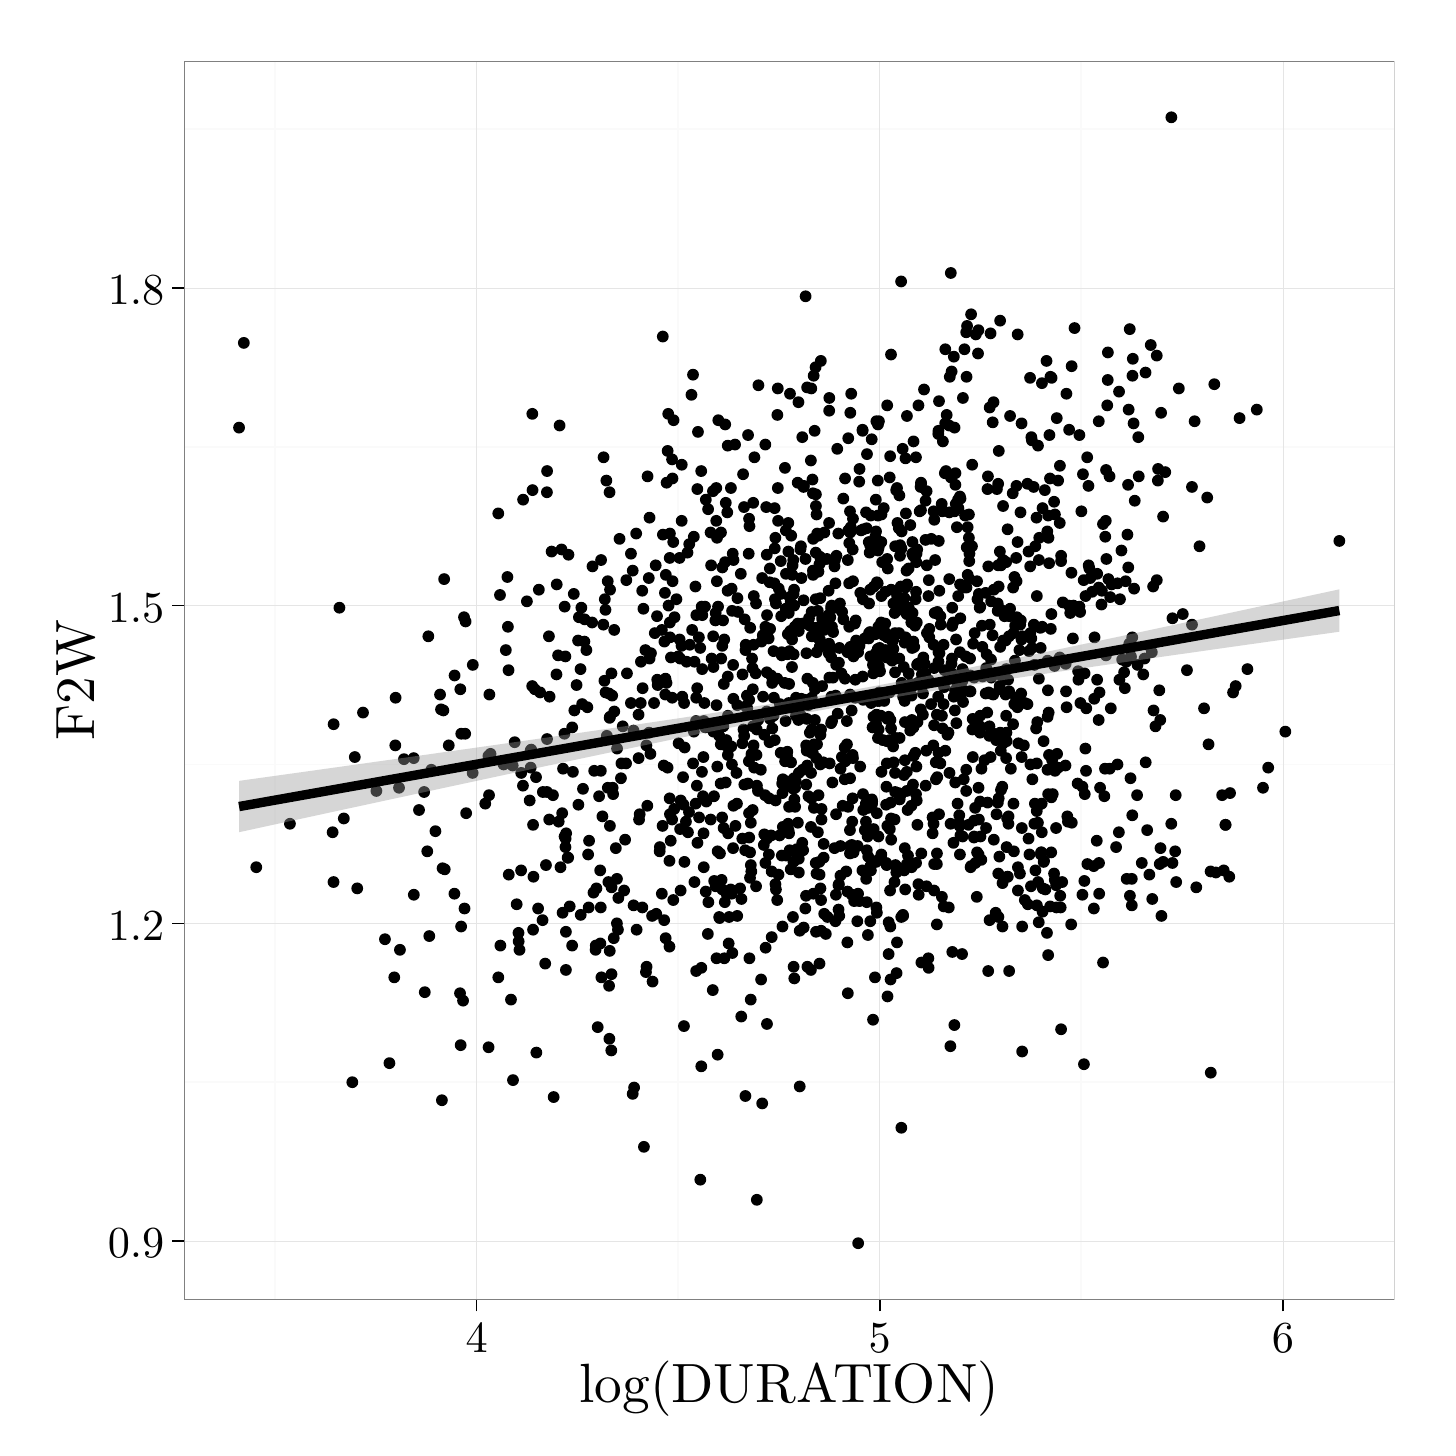
\begin{tikzpicture}[x=1pt,y=1pt]
\definecolor{fillColor}{RGB}{255,255,255}
\path[use as bounding box,fill=fillColor,fill opacity=0.00] (0,0) rectangle (505.89,505.89);
\begin{scope}
\path[clip] (  0.00,  0.00) rectangle (505.89,505.89);
\definecolor{drawColor}{RGB}{255,255,255}
\definecolor{fillColor}{RGB}{255,255,255}

\path[draw=drawColor,line width= 0.6pt,line join=round,line cap=round,fill=fillColor] (  0.00, -0.00) rectangle (505.89,505.89);
\end{scope}
\begin{scope}
\path[clip] ( 56.50, 46.31) rectangle (493.85,493.84);
\definecolor{fillColor}{RGB}{255,255,255}

\path[fill=fillColor] ( 56.50, 46.31) rectangle (493.85,493.84);
\definecolor{drawColor}{gray}{0.98}

\path[draw=drawColor,line width= 0.6pt,line join=round] ( 56.50,124.83) --
	(493.85,124.83);

\path[draw=drawColor,line width= 0.6pt,line join=round] ( 56.50,239.65) --
	(493.85,239.65);

\path[draw=drawColor,line width= 0.6pt,line join=round] ( 56.50,354.47) --
	(493.85,354.47);

\path[draw=drawColor,line width= 0.6pt,line join=round] ( 56.50,469.29) --
	(493.85,469.29);

\path[draw=drawColor,line width= 0.6pt,line join=round] ( 89.37, 46.31) --
	( 89.37,493.84);

\path[draw=drawColor,line width= 0.6pt,line join=round] (235.05, 46.31) --
	(235.05,493.84);

\path[draw=drawColor,line width= 0.6pt,line join=round] (380.73, 46.31) --
	(380.73,493.84);
\definecolor{drawColor}{gray}{0.90}

\path[draw=drawColor,line width= 0.2pt,line join=round] ( 56.50, 67.42) --
	(493.85, 67.42);

\path[draw=drawColor,line width= 0.2pt,line join=round] ( 56.50,182.24) --
	(493.85,182.24);

\path[draw=drawColor,line width= 0.2pt,line join=round] ( 56.50,297.06) --
	(493.85,297.06);

\path[draw=drawColor,line width= 0.2pt,line join=round] ( 56.50,411.88) --
	(493.85,411.88);

\path[draw=drawColor,line width= 0.2pt,line join=round] (162.21, 46.31) --
	(162.21,493.84);

\path[draw=drawColor,line width= 0.2pt,line join=round] (307.89, 46.31) --
	(307.89,493.84);

\path[draw=drawColor,line width= 0.2pt,line join=round] (453.57, 46.31) --
	(453.57,493.84);
\definecolor{fillColor}{RGB}{0,0,0}

\path[fill=fillColor] (211.78,176.88) circle (  2.13);

\path[fill=fillColor] (174.64,154.68) circle (  2.13);

\path[fill=fillColor] (292.11,221.66) circle (  2.13);

\path[fill=fillColor] (292.06,192.57) circle (  2.13);

\path[fill=fillColor] (210.20,140.52) circle (  2.13);

\path[fill=fillColor] (253.48,184.53) circle (  2.13);

\path[fill=fillColor] (235.56,314.28) circle (  2.13);

\path[fill=fillColor] (232.87,219.75) circle (  2.13);

\path[fill=fillColor] (293.26,184.92) circle (  2.13);

\path[fill=fillColor] (241.81,231.99) circle (  2.13);

\path[fill=fillColor] (242.61,220.51) circle (  2.13);

\path[fill=fillColor] (306.84,222.04) circle (  2.13);

\path[fill=fillColor] (225.80,161.19) circle (  2.13);

\path[fill=fillColor] (207.08,187.98) circle (  2.13);

\path[fill=fillColor] (183.26,266.82) circle (  2.13);

\path[fill=fillColor] (275.13,224.34) circle (  2.13);

\path[fill=fillColor] (272.86,234.29) circle (  2.13);

\path[fill=fillColor] (266.16,250.37) circle (  2.13);

\path[fill=fillColor] (223.41,164.63) circle (  2.13);

\path[fill=fillColor] (202.71,187.98) circle (  2.13);

\path[fill=fillColor] (305.15,226.25) circle (  2.13);

\path[fill=fillColor] (210.33,172.29) circle (  2.13);

\path[fill=fillColor] (276.65,230.85) circle (  2.13);

\path[fill=fillColor] (223.91,224.72) circle (  2.13);

\path[fill=fillColor] (243.43,166.16) circle (  2.13);

\path[fill=fillColor] (205.98,144.73) circle (  2.13);

\path[fill=fillColor] (220.74,257.64) circle (  2.13);

\path[fill=fillColor] (321.49,217.83) circle (  2.13);

\path[fill=fillColor] (370.88,200.23) circle (  2.13);

\path[fill=fillColor] (272.74,229.31) circle (  2.13);

\path[fill=fillColor] (283.04,217.07) circle (  2.13);

\path[fill=fillColor] (266.57,204.05) circle (  2.13);

\path[fill=fillColor] (314.38,300.12) circle (  2.13);

\path[fill=fillColor] (216.55,272.56) circle (  2.13);

\path[fill=fillColor] (175.25,239.27) circle (  2.13);

\path[fill=fillColor] (237.19,261.85) circle (  2.13);

\path[fill=fillColor] (227.41,293.23) circle (  2.13);

\path[fill=fillColor] (262.38,300.50) circle (  2.13);

\path[fill=fillColor] (251.48,216.68) circle (  2.13);

\path[fill=fillColor] (321.64,276.01) circle (  2.13);

\path[fill=fillColor] (187.63,338.01) circle (  2.13);

\path[fill=fillColor] (182.62,179.94) circle (  2.13);

\path[fill=fillColor] (284.97,241.94) circle (  2.13);

\path[fill=fillColor] (251.74,169.61) circle (  2.13);

\path[fill=fillColor] (281.75,166.55) circle (  2.13);

\path[fill=fillColor] (249.32,134.78) circle (  2.13);

\path[fill=fillColor] (190.06,119.47) circle (  2.13);

\path[fill=fillColor] (290.67,255.34) circle (  2.13);

\path[fill=fillColor] (134.52,172.67) circle (  2.13);

\path[fill=fillColor] (118.21,242.33) circle (  2.13);

\path[fill=fillColor] (205.28,174.20) circle (  2.13);

\path[fill=fillColor] (195.86,188.36) circle (  2.13);

\path[fill=fillColor] (170.06,162.72) circle (  2.13);

\path[fill=fillColor] (287.83,185.68) circle (  2.13);

\path[fill=fillColor] (287.63,205.97) circle (  2.13);

\path[fill=fillColor] (232.08,221.66) circle (  2.13);

\path[fill=fillColor] (242.02,211.33) circle (  2.13);

\path[fill=fillColor] (211.38,231.23) circle (  2.13);

\path[fill=fillColor] (145.13,177.64) circle (  2.13);

\path[fill=fillColor] (340.53,277.92) circle (  2.13);

\path[fill=fillColor] (371.15,197.93) circle (  2.13);

\path[fill=fillColor] (291.55,209.41) circle (  2.13);

\path[fill=fillColor] (310.70,155.83) circle (  2.13);

\path[fill=fillColor] (219.13,122.91) circle (  2.13);

\path[fill=fillColor] (196.74,174.20) circle (  2.13);

\path[fill=fillColor] (340.72,202.52) circle (  2.13);

\path[fill=fillColor] (258.96,232.38) circle (  2.13);

\path[fill=fillColor] (301.84,228.93) circle (  2.13);

\path[fill=fillColor] (305.05,227.02) circle (  2.13);

\path[fill=fillColor] (257.85,148.56) circle (  2.13);

\path[fill=fillColor] (306.16,162.72) circle (  2.13);

\path[fill=fillColor] (110.55,254.19) circle (  2.13);

\path[fill=fillColor] (286.84,219.75) circle (  2.13);

\path[fill=fillColor] (300.09, 66.65) circle (  2.13);

\path[fill=fillColor] (289.47,279.84) circle (  2.13);

\path[fill=fillColor] (275.30,280.60) circle (  2.13);

\path[fill=fillColor] (207.31,162.72) circle (  2.13);

\path[fill=fillColor] (166.54,137.46) circle (  2.13);

\path[fill=fillColor] (170.81,174.20) circle (  2.13);

\path[fill=fillColor] (235.94,194.10) circle (  2.13);

\path[fill=fillColor] (300.82,238.88) circle (  2.13);

\path[fill=fillColor] (183.81,135.54) circle (  2.13);

\path[fill=fillColor] (250.46,246.92) circle (  2.13);

\path[fill=fillColor] (156.63,181.09) circle (  2.13);

\path[fill=fillColor] (316.94,209.41) circle (  2.13);

\path[fill=fillColor] (243.55,296.68) circle (  2.13);

\path[fill=fillColor] (236.27,282.52) circle (  2.13);

\path[fill=fillColor] (194.03,296.68) circle (  2.13);

\path[fill=fillColor] (270.38,297.82) circle (  2.13);

\path[fill=fillColor] (263.48, 82.34) circle (  2.13);

\path[fill=fillColor] (199.19,292.85) circle (  2.13);

\path[fill=fillColor] (199.77,274.10) circle (  2.13);

\path[fill=fillColor] (330.92,269.12) circle (  2.13);

\path[fill=fillColor] (317.68,230.08) circle (  2.13);

\path[fill=fillColor] (268.62,271.80) circle (  2.13);

\path[fill=fillColor] (194.49,179.18) circle (  2.13);

\path[fill=fillColor] (328.53,203.67) circle (  2.13);

\path[fill=fillColor] (177.36,178.79) circle (  2.13);

\path[fill=fillColor] (270.20,196.40) circle (  2.13);

\path[fill=fillColor] (175.37,125.59) circle (  2.13);

\path[fill=fillColor] (267.14,145.88) circle (  2.13);

\path[fill=fillColor] (241.56,165.01) circle (  2.13);

\path[fill=fillColor] (241.29,303.95) circle (  2.13);

\path[fill=fillColor] (266.65,173.43) circle (  2.13);

\path[fill=fillColor] (313.66,202.91) circle (  2.13);

\path[fill=fillColor] (273.69,240.80) circle (  2.13);

\path[fill=fillColor] (283.02,165.40) circle (  2.13);

\path[fill=fillColor] (297.79,210.56) circle (  2.13);

\path[fill=fillColor] (210.09,159.66) circle (  2.13);

\path[fill=fillColor] (279.89,211.33) circle (  2.13);

\path[fill=fillColor] (280.22,208.65) circle (  2.13);

\path[fill=fillColor] (312.35,277.16) circle (  2.13);

\path[fill=fillColor] (304.48,183.00) circle (  2.13);

\path[fill=fillColor] (324.43,320.79) circle (  2.13);

\path[fill=fillColor] (265.42,117.17) circle (  2.13);

\path[fill=fillColor] (277.02,162.34) circle (  2.13);

\path[fill=fillColor] (261.27,154.68) circle (  2.13);

\path[fill=fillColor] (316.34,184.92) circle (  2.13);

\path[fill=fillColor] (293.70,210.18) circle (  2.13);

\path[fill=fillColor] (276.71,204.44) circle (  2.13);

\path[fill=fillColor] (150.70,201.76) circle (  2.13);

\path[fill=fillColor] (247.56,158.12) circle (  2.13);

\path[fill=fillColor] (351.12,206.35) circle (  2.13);

\path[fill=fillColor] (297.94,218.98) circle (  2.13);

\path[fill=fillColor] (304.69,201.37) circle (  2.13);

\path[fill=fillColor] (296.36,156.98) circle (  2.13);

\path[fill=fillColor] (265.73,264.14) circle (  2.13);

\path[fill=fillColor] (272.74,181.09) circle (  2.13);

\path[fill=fillColor] (278.98,179.56) circle (  2.13);

\path[fill=fillColor] (304.96,225.10) circle (  2.13);

\path[fill=fillColor] (220.04,179.94) circle (  2.13);

\path[fill=fillColor] (254.03,194.49) circle (  2.13);

\path[fill=fillColor] (343.71,219.75) circle (  2.13);

\path[fill=fillColor] (301.89,263.00) circle (  2.13);

\path[fill=fillColor] (354.00,199.08) circle (  2.13);

\path[fill=fillColor] (178.34,236.59) circle (  2.13);

\path[fill=fillColor] (317.67,236.97) circle (  2.13);

\path[fill=fillColor] (264.93,237.73) circle (  2.13);

\path[fill=fillColor] (317.96,223.19) circle (  2.13);

\path[fill=fillColor] (302.99,198.31) circle (  2.13);

\path[fill=fillColor] (260.60,240.80) circle (  2.13);

\path[fill=fillColor] (244.30,202.52) circle (  2.13);

\path[fill=fillColor] (329.79,240.03) circle (  2.13);

\path[fill=fillColor] (311.62,194.10) circle (  2.13);

\path[fill=fillColor] (251.36,253.43) circle (  2.13);

\path[fill=fillColor] (344.15,253.43) circle (  2.13);

\path[fill=fillColor] (368.74,228.93) circle (  2.13);

\path[fill=fillColor] (365.05,218.60) circle (  2.13);

\path[fill=fillColor] (326.98,220.51) circle (  2.13);

\path[fill=fillColor] (282.13,228.17) circle (  2.13);

\path[fill=fillColor] (308.51,236.97) circle (  2.13);

\path[fill=fillColor] (329.12,276.77) circle (  2.13);

\path[fill=fillColor] (222.49,295.91) circle (  2.13);

\path[fill=fillColor] (347.08,165.01) circle (  2.13);

\path[fill=fillColor] (398.29,192.19) circle (  2.13);

\path[fill=fillColor] (311.12,182.62) circle (  2.13);

\path[fill=fillColor] (353.92,220.13) circle (  2.13);

\path[fill=fillColor] (366.83,194.87) circle (  2.13);

\path[fill=fillColor] (415.01,197.16) circle (  2.13);

\path[fill=fillColor] (373.42,143.96) circle (  2.13);

\path[fill=fillColor] (387.18,192.95) circle (  2.13);

\path[fill=fillColor] (320.74,243.86) circle (  2.13);

\path[fill=fillColor] (397.12,198.31) circle (  2.13);

\path[fill=fillColor] (364.63,222.81) circle (  2.13);

\path[fill=fillColor] (254.62,171.52) circle (  2.13);

\path[fill=fillColor] (363.95,225.49) circle (  2.13);

\path[fill=fillColor] (327.57,274.48) circle (  2.13);

\path[fill=fillColor] (346.72,258.40) circle (  2.13);

\path[fill=fillColor] (304.78,261.85) circle (  2.13);

\path[fill=fillColor] (329.01,264.14) circle (  2.13);

\path[fill=fillColor] (377.68,285.19) circle (  2.13);

\path[fill=fillColor] (344.82,289.79) circle (  2.13);

\path[fill=fillColor] (259.09,292.08) circle (  2.13);

\path[fill=fillColor] (258.89,249.98) circle (  2.13);

\path[fill=fillColor] (311.13,256.87) circle (  2.13);

\path[fill=fillColor] (321.52,254.96) circle (  2.13);

\path[fill=fillColor] (334.86,145.49) circle (  2.13);

\path[fill=fillColor] (368.74,170.76) circle (  2.13);

\path[fill=fillColor] (229.15,192.95) circle (  2.13);

\path[fill=fillColor] (265.02,161.95) circle (  2.13);

\path[fill=fillColor] (297.13,207.50) circle (  2.13);

\path[fill=fillColor] (117.31,124.83) circle (  2.13);

\path[fill=fillColor] (149.92,202.14) circle (  2.13);

\path[fill=fillColor] (329.32,221.66) circle (  2.13);

\path[fill=fillColor] (297.43,325.38) circle (  2.13);

\path[fill=fillColor] (286.09,311.99) circle (  2.13);

\path[fill=fillColor] (321.69,269.12) circle (  2.13);

\path[fill=fillColor] (244.17,242.33) circle (  2.13);

\path[fill=fillColor] (210.96,163.87) circle (  2.13);

\path[fill=fillColor] (284.10,223.96) circle (  2.13);

\path[fill=fillColor] (267.10,272.95) circle (  2.13);

\path[fill=fillColor] (316.99,241.18) circle (  2.13);

\path[fill=fillColor] (398.60,278.31) circle (  2.13);

\path[fill=fillColor] (311.80,161.95) circle (  2.13);

\path[fill=fillColor] (243.73,274.10) circle (  2.13);

\path[fill=fillColor] (210.41,256.87) circle (  2.13);

\path[fill=fillColor] (319.90,232.38) circle (  2.13);

\path[fill=fillColor] (206.94,174.97) circle (  2.13);

\path[fill=fillColor] (295.78,200.99) circle (  2.13);

\path[fill=fillColor] (326.45,261.46) circle (  2.13);

\path[fill=fillColor] (338.04,303.57) circle (  2.13);

\path[fill=fillColor] (287.07,267.97) circle (  2.13);

\path[fill=fillColor] (291.97,264.53) circle (  2.13);

\path[fill=fillColor] (247.38,253.04) circle (  2.13);

\path[fill=fillColor] (209.28,249.98) circle (  2.13);

\path[fill=fillColor] (241.39,225.49) circle (  2.13);

\path[fill=fillColor] (258.26,247.30) circle (  2.13);

\path[fill=fillColor] (201.25,292.08) circle (  2.13);

\path[fill=fillColor] (308.39,290.94) circle (  2.13);

\path[fill=fillColor] (247.15,277.92) circle (  2.13);

\path[fill=fillColor] (254.77,315.81) circle (  2.13);

\path[fill=fillColor] (283.79,308.16) circle (  2.13);

\path[fill=fillColor] (269.51,257.25) circle (  2.13);

\path[fill=fillColor] (287.79,288.26) circle (  2.13);

\path[fill=fillColor] (277.92,209.03) circle (  2.13);

\path[fill=fillColor] (317.34,330.36) circle (  2.13);

\path[fill=fillColor] (340.23,313.13) circle (  2.13);

\path[fill=fillColor] (309.05,248.45) circle (  2.13);

\path[fill=fillColor] (233.61,223.57) circle (  2.13);

\path[fill=fillColor] (304.43,302.80) circle (  2.13);

\path[fill=fillColor] (329.23,320.41) circle (  2.13);

\path[fill=fillColor] (289.37,293.61) circle (  2.13);

\path[fill=fillColor] (351.86,312.37) circle (  2.13);

\path[fill=fillColor] (274.01,308.54) circle (  2.13);

\path[fill=fillColor] (333.00,306.63) circle (  2.13);

\path[fill=fillColor] (352.54,272.56) circle (  2.13);

\path[fill=fillColor] (285.12,280.22) circle (  2.13);

\path[fill=fillColor] (291.01,271.03) circle (  2.13);

\path[fill=fillColor] (359.17,242.33) circle (  2.13);

\path[fill=fillColor] (291.87,305.10) circle (  2.13);

\path[fill=fillColor] (324.91,311.60) circle (  2.13);

\path[fill=fillColor] (263.19,297.82) circle (  2.13);

\path[fill=fillColor] (339.23,303.57) circle (  2.13);

\path[fill=fillColor] (235.97,226.64) circle (  2.13);

\path[fill=fillColor] (338.96,278.69) circle (  2.13);

\path[fill=fillColor] (344.18,257.25) circle (  2.13);

\path[fill=fillColor] (267.06,258.79) circle (  2.13);

\path[fill=fillColor] (321.19,315.81) circle (  2.13);

\path[fill=fillColor] (308.28,257.25) circle (  2.13);

\path[fill=fillColor] (371.23,237.35) circle (  2.13);

\path[fill=fillColor] (300.56,282.52) circle (  2.13);

\path[fill=fillColor] (278.27,290.55) circle (  2.13);

\path[fill=fillColor] (352.98,293.23) circle (  2.13);

\path[fill=fillColor] (290.35,295.91) circle (  2.13);

\path[fill=fillColor] (319.12,268.74) circle (  2.13);

\path[fill=fillColor] (357.99,247.30) circle (  2.13);

\path[fill=fillColor] (289.93,280.60) circle (  2.13);

\path[fill=fillColor] (369.71,288.64) circle (  2.13);

\path[fill=fillColor] (387.05,303.57) circle (  2.13);

\path[fill=fillColor] (405.30,282.52) circle (  2.13);

\path[fill=fillColor] (344.02,296.29) circle (  2.13);

\path[fill=fillColor] (380.31,294.76) circle (  2.13);

\path[fill=fillColor] (357.33,305.86) circle (  2.13);

\path[fill=fillColor] (403.57,277.92) circle (  2.13);

\path[fill=fillColor] (380.04,296.68) circle (  2.13);

\path[fill=fillColor] (307.41,289.40) circle (  2.13);

\path[fill=fillColor] (373.42,313.13) circle (  2.13);

\path[fill=fillColor] (300.87,301.65) circle (  2.13);

\path[fill=fillColor] (274.49,279.45) circle (  2.13);

\path[fill=fillColor] (282.10,261.08) circle (  2.13);

\path[fill=fillColor] (311.53,248.45) circle (  2.13);

\path[fill=fillColor] (319.16,268.35) circle (  2.13);

\path[fill=fillColor] (314.88,287.11) circle (  2.13);

\path[fill=fillColor] (270.03,299.36) circle (  2.13);

\path[fill=fillColor] (306.37,286.73) circle (  2.13);

\path[fill=fillColor] (286.28,284.81) circle (  2.13);

\path[fill=fillColor] (359.97,246.54) circle (  2.13);

\path[fill=fillColor] (362.34,239.65) circle (  2.13);

\path[fill=fillColor] (247.80,251.51) circle (  2.13);

\path[fill=fillColor] (359.12,284.81) circle (  2.13);

\path[fill=fillColor] (252.92,302.42) circle (  2.13);

\path[fill=fillColor] (310.64,256.11) circle (  2.13);

\path[fill=fillColor] (290.35,296.68) circle (  2.13);

\path[fill=fillColor] (351.30,316.58) circle (  2.13);

\path[fill=fillColor] (352.49,313.52) circle (  2.13);

\path[fill=fillColor] (371.20,329.98) circle (  2.13);

\path[fill=fillColor] (390.93,343.75) circle (  2.13);

\path[fill=fillColor] (252.99,271.42) circle (  2.13);

\path[fill=fillColor] (287.99,290.94) circle (  2.13);

\path[fill=fillColor] (299.20,291.70) circle (  2.13);

\path[fill=fillColor] (229.17,288.26) circle (  2.13);

\path[fill=fillColor] (265.64,286.34) circle (  2.13);

\path[fill=fillColor] (286.33,314.67) circle (  2.13);

\path[fill=fillColor] (276.28,308.16) circle (  2.13);

\path[fill=fillColor] (348.66,286.34) circle (  2.13);

\path[fill=fillColor] (290.62,289.40) circle (  2.13);

\path[fill=fillColor] (324.29,272.56) circle (  2.13);

\path[fill=fillColor] (265.16,284.05) circle (  2.13);

\path[fill=fillColor] (233.74,292.85) circle (  2.13);

\path[fill=fillColor] (305.33,286.73) circle (  2.13);

\path[fill=fillColor] (266.01,210.56) circle (  2.13);

\path[fill=fillColor] (245.02,193.72) circle (  2.13);

\path[fill=fillColor] (243.41,130.57) circle (  2.13);

\path[fill=fillColor] (110.19,215.15) circle (  2.13);

\path[fill=fillColor] (156.23,156.98) circle (  2.13);

\path[fill=fillColor] (251.91,189.89) circle (  2.13);

\path[fill=fillColor] (172.78,280.98) circle (  2.13);

\path[fill=fillColor] (158.24,291.32) circle (  2.13);

\path[fill=fillColor] (245.97,189.89) circle (  2.13);

\path[fill=fillColor] (114.24,220.13) circle (  2.13);

\path[fill=fillColor] (193.95,250.75) circle (  2.13);

\path[fill=fillColor] (166.71,228.55) circle (  2.13);

\path[fill=fillColor] (275.35,208.65) circle (  2.13);

\path[fill=fillColor] (285.76,228.55) circle (  2.13);

\path[fill=fillColor] (157.32,154.30) circle (  2.13);

\path[fill=fillColor] (218.94,188.74) circle (  2.13);

\path[fill=fillColor] (328.68,235.06) circle (  2.13);

\path[fill=fillColor] (278.31,218.60) circle (  2.13);

\path[fill=fillColor] (228.44,209.79) circle (  2.13);

\path[fill=fillColor] (199.84,185.30) circle (  2.13);

\path[fill=fillColor] (212.53,209.41) circle (  2.13);

\path[fill=fillColor] (147.34,215.54) circle (  2.13);

\path[fill=fillColor] (145.87,237.73) circle (  2.13);

\path[fill=fillColor] (289.80,240.03) circle (  2.13);

\path[fill=fillColor] (139.53,192.57) circle (  2.13);

\path[fill=fillColor] (189.81,228.55) circle (  2.13);

\path[fill=fillColor] (211.55,228.93) circle (  2.13);

\path[fill=fillColor] (186.16,229.70) circle (  2.13);

\path[fill=fillColor] (270.38,194.49) circle (  2.13);

\path[fill=fillColor] (156.46,138.22) circle (  2.13);

\path[fill=fillColor] (240.93,197.16) circle (  2.13);

\path[fill=fillColor] (253.10,214.77) circle (  2.13);

\path[fill=fillColor] (165.35,225.49) circle (  2.13);

\path[fill=fillColor] (284.86,179.18) circle (  2.13);

\path[fill=fillColor] (312.81,281.37) circle (  2.13);

\path[fill=fillColor] ( 94.77,218.22) circle (  2.13);

\path[fill=fillColor] (249.89,184.53) circle (  2.13);

\path[fill=fillColor] (119.08,194.87) circle (  2.13);

\path[fill=fillColor] (281.25,192.19) circle (  2.13);

\path[fill=fillColor] (187.01,167.69) circle (  2.13);

\path[fill=fillColor] (143.49,157.36) circle (  2.13);

\path[fill=fillColor] (243.06, 89.61) circle (  2.13);

\path[fill=fillColor] (132.47,162.72) circle (  2.13);

\path[fill=fillColor] (130.72,131.72) circle (  2.13);

\path[fill=fillColor] (193.29,186.06) circle (  2.13);

\path[fill=fillColor] (110.52,197.16) circle (  2.13);

\path[fill=fillColor] (214.38,234.67) circle (  2.13);

\path[fill=fillColor] (177.41,175.73) circle (  2.13);

\path[fill=fillColor] (195.30,205.97) circle (  2.13);

\path[fill=fillColor] (300.55,190.28) circle (  2.13);

\path[fill=fillColor] (303.20,189.89) circle (  2.13);

\path[fill=fillColor] (221.14,221.66) circle (  2.13);

\path[fill=fillColor] (312.94,240.41) circle (  2.13);

\path[fill=fillColor] (275.73,201.76) circle (  2.13);

\path[fill=fillColor] (206.88,201.37) circle (  2.13);

\path[fill=fillColor] (310.39,203.29) circle (  2.13);

\path[fill=fillColor] (149.68,118.32) circle (  2.13);

\path[fill=fillColor] (286.72,179.56) circle (  2.13);

\path[fill=fillColor] (184.44,187.60) circle (  2.13);

\path[fill=fillColor] (255.75,217.45) circle (  2.13);

\path[fill=fillColor] (209.83,197.16) circle (  2.13);

\path[fill=fillColor] (205.51,194.87) circle (  2.13);

\path[fill=fillColor] (283.90,192.95) circle (  2.13);

\path[fill=fillColor] (204.45,193.34) circle (  2.13);

\path[fill=fillColor] (193.14,222.04) circle (  2.13);

\path[fill=fillColor] (175.98,247.69) circle (  2.13);

\path[fill=fillColor] (250.93,220.51) circle (  2.13);

\path[fill=fillColor] (263.20,195.63) circle (  2.13);

\path[fill=fillColor] (271.05,375.52) circle (  2.13);

\path[fill=fillColor] (191.88,218.98) circle (  2.13);

\path[fill=fillColor] (293.00,187.21) circle (  2.13);

\path[fill=fillColor] (228.37,208.26) circle (  2.13);

\path[fill=fillColor] (312.02,212.47) circle (  2.13);

\path[fill=fillColor] (280.41,180.71) circle (  2.13);

\path[fill=fillColor] (272.13,301.27) circle (  2.13);

\path[fill=fillColor] (237.01,225.10) circle (  2.13);

\path[fill=fillColor] (143.26,229.70) circle (  2.13);

\path[fill=fillColor] (126.01,230.08) circle (  2.13);

\path[fill=fillColor] (268.84,200.99) circle (  2.13);

\path[fill=fillColor] (212.93,198.31) circle (  2.13);

\path[fill=fillColor] (251.00,194.49) circle (  2.13);

\path[fill=fillColor] (248.91,261.08) circle (  2.13);

\path[fill=fillColor] (236.82,235.06) circle (  2.13);

\path[fill=fillColor] (195.12,205.97) circle (  2.13);

\path[fill=fillColor] (260.73,213.24) circle (  2.13);

\path[fill=fillColor] (248.58,195.63) circle (  2.13);

\path[fill=fillColor] (280.02,237.73) circle (  2.13);

\path[fill=fillColor] (178.97,231.99) circle (  2.13);

\path[fill=fillColor] (295.24,234.29) circle (  2.13);

\path[fill=fillColor] (181.40,226.64) circle (  2.13);

\path[fill=fillColor] (263.90,230.08) circle (  2.13);

\path[fill=fillColor] (289.01,184.53) circle (  2.13);

\path[fill=fillColor] (336.63,221.28) circle (  2.13);

\path[fill=fillColor] (266.18,214.39) circle (  2.13);

\path[fill=fillColor] (302.86,225.49) circle (  2.13);

\path[fill=fillColor] (311.71,181.09) circle (  2.13);

\path[fill=fillColor] (315.70,108.37) circle (  2.13);

\path[fill=fillColor] (248.91,169.61) circle (  2.13);

\path[fill=fillColor] (271.31,199.84) circle (  2.13);

\path[fill=fillColor] (220.92,219.75) circle (  2.13);

\path[fill=fillColor] (266.45,228.55) circle (  2.13);

\path[fill=fillColor] (314.13,175.35) circle (  2.13);

\path[fill=fillColor] (334.11,171.90) circle (  2.13);

\path[fill=fillColor] (307.42,213.62) circle (  2.13);

\path[fill=fillColor] (328.56,207.50) circle (  2.13);

\path[fill=fillColor] (366.13,207.12) circle (  2.13);

\path[fill=fillColor] (354.65,165.01) circle (  2.13);

\path[fill=fillColor] (388.58,168.08) circle (  2.13);

\path[fill=fillColor] (409.68,184.92) circle (  2.13);

\path[fill=fillColor] (352.24,181.09) circle (  2.13);

\path[fill=fillColor] (406.37,191.04) circle (  2.13);

\path[fill=fillColor] (359.35,181.09) circle (  2.13);

\path[fill=fillColor] (359.35,135.93) circle (  2.13);

\path[fill=fillColor] (368.32,178.79) circle (  2.13);

\path[fill=fillColor] (324.10,276.01) circle (  2.13);

\path[fill=fillColor] (329.12,243.86) circle (  2.13);

\path[fill=fillColor] (275.00,261.85) circle (  2.13);

\path[fill=fillColor] (330.95,282.90) circle (  2.13);

\path[fill=fillColor] (359.24,216.68) circle (  2.13);

\path[fill=fillColor] (305.47,147.41) circle (  2.13);

\path[fill=fillColor] (273.77,217.07) circle (  2.13);

\path[fill=fillColor] (344.97,282.13) circle (  2.13);

\path[fill=fillColor] (284.12,246.92) circle (  2.13);

\path[fill=fillColor] (305.30,253.04) circle (  2.13);

\path[fill=fillColor] (336.05,268.35) circle (  2.13);

\path[fill=fillColor] (366.41,225.49) circle (  2.13);

\path[fill=fillColor] (293.15,276.39) circle (  2.13);

\path[fill=fillColor] (244.22,214.77) circle (  2.13);

\path[fill=fillColor] (258.23,212.86) circle (  2.13);

\path[fill=fillColor] (358.64,290.17) circle (  2.13);

\path[fill=fillColor] (256.39,184.92) circle (  2.13);

\path[fill=fillColor] (225.63,184.92) circle (  2.13);

\path[fill=fillColor] (188.46,219.75) circle (  2.13);

\path[fill=fillColor] (176.70,189.13) circle (  2.13);

\path[fill=fillColor] (197.01,236.97) circle (  2.13);

\path[fill=fillColor] (157.85,187.60) circle (  2.13);

\path[fill=fillColor] (309.39,286.34) circle (  2.13);

\path[fill=fillColor] (280.38,298.97) circle (  2.13);

\path[fill=fillColor] (315.09,227.02) circle (  2.13);

\path[fill=fillColor] (261.03,207.88) circle (  2.13);

\path[fill=fillColor] (187.67,248.83) circle (  2.13);

\path[fill=fillColor] (230.39,264.91) circle (  2.13);

\path[fill=fillColor] (182.31,267.97) circle (  2.13);

\path[fill=fillColor] (344.15,251.13) circle (  2.13);

\path[fill=fillColor] (239.06,319.26) circle (  2.13);

\path[fill=fillColor] (331.32,273.71) circle (  2.13);

\path[fill=fillColor] (254.91,275.63) circle (  2.13);

\path[fill=fillColor] (150.21,259.17) circle (  2.13);

\path[fill=fillColor] (141.41,223.19) circle (  2.13);

\path[fill=fillColor] (368.56,277.16) circle (  2.13);

\path[fill=fillColor] (308.47,207.12) circle (  2.13);

\path[fill=fillColor] (252.22,246.54) circle (  2.13);

\path[fill=fillColor] (312.84,297.82) circle (  2.13);

\path[fill=fillColor] (321.28,290.94) circle (  2.13);

\path[fill=fillColor] (368.66,266.44) circle (  2.13);

\path[fill=fillColor] (200.07,296.29) circle (  2.13);

\path[fill=fillColor] (319.30,290.94) circle (  2.13);

\path[fill=fillColor] (287.50,240.41) circle (  2.13);

\path[fill=fillColor] (335.11,266.44) circle (  2.13);

\path[fill=fillColor] (328.14,240.41) circle (  2.13);

\path[fill=fillColor] (253.04,257.25) circle (  2.13);

\path[fill=fillColor] (302.50,215.92) circle (  2.13);

\path[fill=fillColor] (230.00,183.39) circle (  2.13);

\path[fill=fillColor] (408.91,266.44) circle (  2.13);

\path[fill=fillColor] (121.17,258.40) circle (  2.13);

\path[fill=fillColor] (302.90,218.98) circle (  2.13);

\path[fill=fillColor] (312.40,277.92) circle (  2.13);

\path[fill=fillColor] (325.50,300.50) circle (  2.13);

\path[fill=fillColor] (194.30,278.69) circle (  2.13);

\path[fill=fillColor] (318.31,310.46) circle (  2.13);

\path[fill=fillColor] (191.08,272.18) circle (  2.13);

\path[fill=fillColor] (297.74,259.17) circle (  2.13);

\path[fill=fillColor] (352.17,231.61) circle (  2.13);

\path[fill=fillColor] (299.00,263.76) circle (  2.13);

\path[fill=fillColor] (263.05,272.56) circle (  2.13);

\path[fill=fillColor] (254.24,246.16) circle (  2.13);

\path[fill=fillColor] (252.23,233.14) circle (  2.13);

\path[fill=fillColor] (351.63,244.62) circle (  2.13);

\path[fill=fillColor] (210.94,272.56) circle (  2.13);

\path[fill=fillColor] (352.45,333.04) circle (  2.13);

\path[fill=fillColor] (368.56,256.87) circle (  2.13);

\path[fill=fillColor] (358.75,330.74) circle (  2.13);

\path[fill=fillColor] (380.04,358.68) circle (  2.13);

\path[fill=fillColor] (364.11,318.49) circle (  2.13);

\path[fill=fillColor] (397.69,310.84) circle (  2.13);

\path[fill=fillColor] (368.86,321.55) circle (  2.13);

\path[fill=fillColor] (304.42,318.88) circle (  2.13);

\path[fill=fillColor] (357.29,340.31) circle (  2.13);

\path[fill=fillColor] (281.32,232.38) circle (  2.13);

\path[fill=fillColor] (290.37,278.31) circle (  2.13);

\path[fill=fillColor] (306.48,279.84) circle (  2.13);

\path[fill=fillColor] (351.70,230.46) circle (  2.13);

\path[fill=fillColor] (181.95,245.01) circle (  2.13);

\path[fill=fillColor] (202.24,260.32) circle (  2.13);

\path[fill=fillColor] (249.91,249.98) circle (  2.13);

\path[fill=fillColor] (226.61,287.11) circle (  2.13);

\path[fill=fillColor] (272.48,279.07) circle (  2.13);

\path[fill=fillColor] (313.43,272.95) circle (  2.13);

\path[fill=fillColor] (204.09,311.22) circle (  2.13);

\path[fill=fillColor] (226.33,261.85) circle (  2.13);

\path[fill=fillColor] (230.47,270.65) circle (  2.13);

\path[fill=fillColor] (251.00,282.52) circle (  2.13);

\path[fill=fillColor] (236.54,264.14) circle (  2.13);

\path[fill=fillColor] (307.52,318.11) circle (  2.13);

\path[fill=fillColor] (230.08,284.05) circle (  2.13);

\path[fill=fillColor] (320.34,282.13) circle (  2.13);

\path[fill=fillColor] (277.20,289.40) circle (  2.13);

\path[fill=fillColor] (307.49,252.28) circle (  2.13);

\path[fill=fillColor] (144.39,208.26) circle (  2.13);

\path[fill=fillColor] (310.79,310.46) circle (  2.13);

\path[fill=fillColor] (156.34,266.82) circle (  2.13);

\path[fill=fillColor] (156.67,250.75) circle (  2.13);

\path[fill=fillColor] (303.72,206.35) circle (  2.13);

\path[fill=fillColor] (183.69,235.06) circle (  2.13);

\path[fill=fillColor] (275.89,287.87) circle (  2.13);

\path[fill=fillColor] (301.73,271.42) circle (  2.13);

\path[fill=fillColor] (191.67,279.07) circle (  2.13);

\path[fill=fillColor] (213.44,191.42) circle (  2.13);

\path[fill=fillColor] (167.24,243.48) circle (  2.13);

\path[fill=fillColor] (144.78,285.96) circle (  2.13);

\path[fill=fillColor] (134.18,231.23) circle (  2.13);

\path[fill=fillColor] (157.67,292.85) circle (  2.13);

\path[fill=fillColor] (311.98,252.66) circle (  2.13);

\path[fill=fillColor] (256.43,261.08) circle (  2.13);

\path[fill=fillColor] (243.78,293.61) circle (  2.13);

\path[fill=fillColor] (234.42,299.36) circle (  2.13);

\path[fill=fillColor] (296.36,313.52) circle (  2.13);

\path[fill=fillColor] (279.43,257.25) circle (  2.13);

\path[fill=fillColor] (268.23,256.11) circle (  2.13);

\path[fill=fillColor] (188.35,285.96) circle (  2.13);

\path[fill=fillColor] (305.56,272.56) circle (  2.13);

\path[fill=fillColor] (193.46,238.12) circle (  2.13);

\path[fill=fillColor] (319.58,281.75) circle (  2.13);

\path[fill=fillColor] (274.85,280.22) circle (  2.13);

\path[fill=fillColor] (187.65,229.70) circle (  2.13);

\path[fill=fillColor] (263.94,255.72) circle (  2.13);

\path[fill=fillColor] (237.31,204.44) circle (  2.13);

\path[fill=fillColor] (235.76,277.92) circle (  2.13);

\path[fill=fillColor] (218.92,251.90) circle (  2.13);

\path[fill=fillColor] (329.11,280.22) circle (  2.13);

\path[fill=fillColor] (268.11,305.48) circle (  2.13);

\path[fill=fillColor] (336.86,280.22) circle (  2.13);

\path[fill=fillColor] (235.06,278.69) circle (  2.13);

\path[fill=fillColor] (318.34,272.56) circle (  2.13);

\path[fill=fillColor] (254.37,303.18) circle (  2.13);

\path[fill=fillColor] (272.29,293.23) circle (  2.13);

\path[fill=fillColor] (297.28,282.13) circle (  2.13);

\path[fill=fillColor] (281.74,270.65) circle (  2.13);

\path[fill=fillColor] (261.49,200.99) circle (  2.13);

\path[fill=fillColor] (268.07,247.69) circle (  2.13);

\path[fill=fillColor] (200.66,230.85) circle (  2.13);

\path[fill=fillColor] (337.04,269.88) circle (  2.13);

\path[fill=fillColor] (341.94,213.24) circle (  2.13);

\path[fill=fillColor] (353.37,264.91) circle (  2.13);

\path[fill=fillColor] (235.58,284.81) circle (  2.13);

\path[fill=fillColor] (291.04,287.49) circle (  2.13);

\path[fill=fillColor] (336.02,225.49) circle (  2.13);

\path[fill=fillColor] (277.04,227.02) circle (  2.13);

\path[fill=fillColor] (261.98,223.19) circle (  2.13);

\path[fill=fillColor] (262.04,266.82) circle (  2.13);

\path[fill=fillColor] (296.01,255.34) circle (  2.13);

\path[fill=fillColor] (330.94,261.46) circle (  2.13);

\path[fill=fillColor] (310.08,279.45) circle (  2.13);

\path[fill=fillColor] (341.38,252.28) circle (  2.13);

\path[fill=fillColor] (254.48,239.65) circle (  2.13);

\path[fill=fillColor] (260.02,259.93) circle (  2.13);

\path[fill=fillColor] (304.02,287.11) circle (  2.13);

\path[fill=fillColor] (324.70,244.62) circle (  2.13);

\path[fill=fillColor] (335.58,254.58) circle (  2.13);

\path[fill=fillColor] (334.62,264.14) circle (  2.13);

\path[fill=fillColor] (244.34,255.34) circle (  2.13);

\path[fill=fillColor] (260.66,222.04) circle (  2.13);

\path[fill=fillColor] (331.57,244.62) circle (  2.13);

\path[fill=fillColor] (345.75,241.18) circle (  2.13);

\path[fill=fillColor] (338.24,234.29) circle (  2.13);

\path[fill=fillColor] (307.28,264.91) circle (  2.13);

\path[fill=fillColor] (387.04,363.66) circle (  2.13);

\path[fill=fillColor] (383.31,340.31) circle (  2.13);

\path[fill=fillColor] (272.12,313.13) circle (  2.13);

\path[fill=fillColor] (331.41,344.90) circle (  2.13);

\path[fill=fillColor] (397.39,322.70) circle (  2.13);

\path[fill=fillColor] (308.47,320.02) circle (  2.13);

\path[fill=fillColor] (369.58,379.73) circle (  2.13);

\path[fill=fillColor] (407.99,387.39) circle (  2.13);

\path[fill=fillColor] (381.32,344.52) circle (  2.13);

\path[fill=fillColor] (397.83,367.87) circle (  2.13);

\path[fill=fillColor] (382.85,350.64) circle (  2.13);

\path[fill=fillColor] (335.25,344.90) circle (  2.13);

\path[fill=fillColor] (377.15,308.92) circle (  2.13);

\path[fill=fillColor] (173.53,289.40) circle (  2.13);

\path[fill=fillColor] (313.38,287.11) circle (  2.13);

\path[fill=fillColor] (192.53,202.52) circle (  2.13);

\path[fill=fillColor] (177.72,172.67) circle (  2.13);

\path[fill=fillColor] (197.54,259.17) circle (  2.13);

\path[fill=fillColor] (257.43,194.87) circle (  2.13);

\path[fill=fillColor] (281.01,187.60) circle (  2.13);

\path[fill=fillColor] (278.98,123.30) circle (  2.13);

\path[fill=fillColor] (311.87,225.87) circle (  2.13);

\path[fill=fillColor] (222.11,187.98) circle (  2.13);

\path[fill=fillColor] (158.44,222.04) circle (  2.13);

\path[fill=fillColor] (249.32,208.26) circle (  2.13);

\path[fill=fillColor] (237.86,218.98) circle (  2.13);

\path[fill=fillColor] (273.87,255.34) circle (  2.13);

\path[fill=fillColor] (206.48,228.17) circle (  2.13);

\path[fill=fillColor] (306.85,186.06) circle (  2.13);

\path[fill=fillColor] (213.29,179.94) circle (  2.13);

\path[fill=fillColor] (274.03,206.73) circle (  2.13);

\path[fill=fillColor] (227.13,185.68) circle (  2.13);

\path[fill=fillColor] (205.21,172.67) circle (  2.13);

\path[fill=fillColor] (182.76,199.08) circle (  2.13);

\path[fill=fillColor] (215.88,212.47) circle (  2.13);

\path[fill=fillColor] (270.84,190.66) circle (  2.13);

\path[fill=fillColor] (231.90,204.82) circle (  2.13);

\path[fill=fillColor] (210.89,136.31) circle (  2.13);

\path[fill=fillColor] (321.85,196.40) circle (  2.13);

\path[fill=fillColor] (221.52,261.85) circle (  2.13);

\path[fill=fillColor] (286.05,204.44) circle (  2.13);

\path[fill=fillColor] (222.68,101.48) circle (  2.13);

\path[fill=fillColor] (310.24,204.05) circle (  2.13);

\path[fill=fillColor] (356.36,208.26) circle (  2.13);

\path[fill=fillColor] (267.15,212.86) circle (  2.13);

\path[fill=fillColor] (253.30,174.97) circle (  2.13);

\path[fill=fillColor] (301.94,223.19) circle (  2.13);

\path[fill=fillColor] (216.22,240.03) circle (  2.13);

\path[fill=fillColor] (256.12,236.59) circle (  2.13);

\path[fill=fillColor] (315.38,228.55) circle (  2.13);

\path[fill=fillColor] (218.62,120.62) circle (  2.13);

\path[fill=fillColor] (223.57,246.54) circle (  2.13);

\path[fill=fillColor] (281.69,239.27) circle (  2.13);

\path[fill=fillColor] (277.32,224.34) circle (  2.13);

\path[fill=fillColor] (344.29,213.62) circle (  2.13);

\path[fill=fillColor] (339.15,237.73) circle (  2.13);

\path[fill=fillColor] (337.04,214.00) circle (  2.13);

\path[fill=fillColor] (263.44,252.28) circle (  2.13);

\path[fill=fillColor] (363.04,234.29) circle (  2.13);

\path[fill=fillColor] (303.51,213.62) circle (  2.13);

\path[fill=fillColor] (296.19,175.35) circle (  2.13);

\path[fill=fillColor] (250.03,184.15) circle (  2.13);

\path[fill=fillColor] (290.78,233.14) circle (  2.13);

\path[fill=fillColor] (335.17,233.14) circle (  2.13);

\path[fill=fillColor] (281.51,244.62) circle (  2.13);

\path[fill=fillColor] (322.91,207.50) circle (  2.13);

\path[fill=fillColor] (367.73,194.49) circle (  2.13);

\path[fill=fillColor] (311.97,220.13) circle (  2.13);

\path[fill=fillColor] (372.37,238.50) circle (  2.13);

\path[fill=fillColor] (390.98,238.12) circle (  2.13);

\path[fill=fillColor] (402.58,204.05) circle (  2.13);

\path[fill=fillColor] (381.98,228.93) circle (  2.13);

\path[fill=fillColor] (394.30,215.15) circle (  2.13);

\path[fill=fillColor] (286.69,190.66) circle (  2.13);

\path[fill=fillColor] (393.30,209.79) circle (  2.13);

\path[fill=fillColor] (369.85,207.88) circle (  2.13);

\path[fill=fillColor] (322.94,168.08) circle (  2.13);

\path[fill=fillColor] (344.64,238.12) circle (  2.13);

\path[fill=fillColor] (331.15,267.59) circle (  2.13);

\path[fill=fillColor] (353.57,257.25) circle (  2.13);

\path[fill=fillColor] (292.20,296.29) circle (  2.13);

\path[fill=fillColor] (357.45,292.85) circle (  2.13);

\path[fill=fillColor] (351.24,267.97) circle (  2.13);

\path[fill=fillColor] (317.09,194.49) circle (  2.13);

\path[fill=fillColor] (214.55,240.03) circle (  2.13);

\path[fill=fillColor] (295.32,270.65) circle (  2.13);

\path[fill=fillColor] (354.65,266.06) circle (  2.13);

\path[fill=fillColor] (324.95,287.11) circle (  2.13);

\path[fill=fillColor] (300.08,280.22) circle (  2.13);

\path[fill=fillColor] (387.30,265.67) circle (  2.13);

\path[fill=fillColor] (256.30,225.49) circle (  2.13);

\path[fill=fillColor] (316.66,235.82) circle (  2.13);

\path[fill=fillColor] (232.36,212.09) circle (  2.13);

\path[fill=fillColor] (296.26,193.72) circle (  2.13);

\path[fill=fillColor] (199.00,225.10) circle (  2.13);

\path[fill=fillColor] (210.29,256.49) circle (  2.13);

\path[fill=fillColor] (129.10,176.50) circle (  2.13);

\path[fill=fillColor] (211.21,264.53) circle (  2.13);

\path[fill=fillColor] (285.04,200.23) circle (  2.13);

\path[fill=fillColor] (340.69,266.06) circle (  2.13);

\path[fill=fillColor] (256.48,299.74) circle (  2.13);

\path[fill=fillColor] (330.60,252.66) circle (  2.13);

\path[fill=fillColor] (366.28,207.88) circle (  2.13);

\path[fill=fillColor] (267.83,207.12) circle (  2.13);

\path[fill=fillColor] (245.24,226.25) circle (  2.13);

\path[fill=fillColor] (304.53,202.91) circle (  2.13);

\path[fill=fillColor] (307.70,262.61) circle (  2.13);

\path[fill=fillColor] (286.67,252.28) circle (  2.13);

\path[fill=fillColor] (244.52,261.85) circle (  2.13);

\path[fill=fillColor] (268.67,214.00) circle (  2.13);

\path[fill=fillColor] (260.25,232.76) circle (  2.13);

\path[fill=fillColor] (194.38,212.86) circle (  2.13);

\path[fill=fillColor] (342.46,204.05) circle (  2.13);

\path[fill=fillColor] (210.99,195.25) circle (  2.13);

\path[fill=fillColor] (223.64,166.55) circle (  2.13);

\path[fill=fillColor] (182.62,217.83) circle (  2.13);

\path[fill=fillColor] (297.13,215.92) circle (  2.13);

\path[fill=fillColor] (261.01,198.70) circle (  2.13);

\path[fill=fillColor] (314.69,229.31) circle (  2.13);

\path[fill=fillColor] (202.86,212.09) circle (  2.13);

\path[fill=fillColor] (278.13,205.97) circle (  2.13);

\path[fill=fillColor] (252.45,248.45) circle (  2.13);

\path[fill=fillColor] (297.81,192.57) circle (  2.13);

\path[fill=fillColor] (278.65,200.61) circle (  2.13);

\path[fill=fillColor] (323.48,257.64) circle (  2.13);

\path[fill=fillColor] (298.64,190.28) circle (  2.13);

\path[fill=fillColor] (319.32,224.72) circle (  2.13);

\path[fill=fillColor] (231.98,227.40) circle (  2.13);

\path[fill=fillColor] (286.46,194.87) circle (  2.13);

\path[fill=fillColor] (320.14,242.71) circle (  2.13);

\path[fill=fillColor] (327.56,203.67) circle (  2.13);

\path[fill=fillColor] (225.02,243.48) circle (  2.13);

\path[fill=fillColor] (293.74,238.12) circle (  2.13);

\path[fill=fillColor] (301.63,201.37) circle (  2.13);

\path[fill=fillColor] (154.20,192.95) circle (  2.13);

\path[fill=fillColor] (292.98,196.02) circle (  2.13);

\path[fill=fillColor] (321.14,238.88) circle (  2.13);

\path[fill=fillColor] (336.73,217.45) circle (  2.13);

\path[fill=fillColor] (312.72,246.16) circle (  2.13);

\path[fill=fillColor] (160.79,236.59) circle (  2.13);

\path[fill=fillColor] (194.00,213.62) circle (  2.13);

\path[fill=fillColor] (248.06,197.55) circle (  2.13);

\path[fill=fillColor] (276.53,184.53) circle (  2.13);

\path[fill=fillColor] (257.92,191.04) circle (  2.13);

\path[fill=fillColor] (310.63,217.45) circle (  2.13);

\path[fill=fillColor] (274.42,233.52) circle (  2.13);

\path[fill=fillColor] (306.61,204.44) circle (  2.13);

\path[fill=fillColor] (334.53,211.33) circle (  2.13);

\path[fill=fillColor] (389.05,228.17) circle (  2.13);

\path[fill=fillColor] (344.60,205.20) circle (  2.13);

\path[fill=fillColor] (295.85,241.56) circle (  2.13);

\path[fill=fillColor] (321.39,275.63) circle (  2.13);

\path[fill=fillColor] (361.66,212.86) circle (  2.13);

\path[fill=fillColor] (263.50,231.99) circle (  2.13);

\path[fill=fillColor] (277.54,233.52) circle (  2.13);

\path[fill=fillColor] (336.56,218.60) circle (  2.13);

\path[fill=fillColor] (385.21,202.91) circle (  2.13);

\path[fill=fillColor] (360.32,190.66) circle (  2.13);

\path[fill=fillColor] (324.47,231.99) circle (  2.13);

\path[fill=fillColor] (341.98,213.62) circle (  2.13);

\path[fill=fillColor] (414.64,208.26) circle (  2.13);

\path[fill=fillColor] (274.78,218.22) circle (  2.13);

\path[fill=fillColor] (360.31,261.85) circle (  2.13);

\path[fill=fillColor] (403.99,240.41) circle (  2.13);

\path[fill=fillColor] (425.08,259.93) circle (  2.13);

\path[fill=fillColor] (434.48,229.31) circle (  2.13);

\path[fill=fillColor] (395.49,277.54) circle (  2.13);

\path[fill=fillColor] (310.45,240.03) circle (  2.13);

\path[fill=fillColor] (454.45,251.51) circle (  2.13);

\path[fill=fillColor] (382.43,237.35) circle (  2.13);

\path[fill=fillColor] (371.98,243.48) circle (  2.13);

\path[fill=fillColor] (391.39,259.93) circle (  2.13);

\path[fill=fillColor] (278.51,255.72) circle (  2.13);

\path[fill=fillColor] (260.71,263.00) circle (  2.13);

\path[fill=fillColor] (275.84,240.41) circle (  2.13);

\path[fill=fillColor] (208.81,265.67) circle (  2.13);

\path[fill=fillColor] (150.49,306.63) circle (  2.13);

\path[fill=fillColor] (132.84,246.54) circle (  2.13);

\path[fill=fillColor] (225.22,279.84) circle (  2.13);

\path[fill=fillColor] (277.64,263.76) circle (  2.13);

\path[fill=fillColor] (413.27,473.50) circle (  2.13);

\path[fill=fillColor] (259.38,280.98) circle (  2.13);

\path[fill=fillColor] (269.07,252.66) circle (  2.13);

\path[fill=fillColor] (316.33,264.14) circle (  2.13);

\path[fill=fillColor] (173.84,199.84) circle (  2.13);

\path[fill=fillColor] (310.19,225.10) circle (  2.13);

\path[fill=fillColor] (307.25,249.22) circle (  2.13);

\path[fill=fillColor] (276.90,234.67) circle (  2.13);

\path[fill=fillColor] (231.46,366.34) circle (  2.13);

\path[fill=fillColor] (289.58,283.28) circle (  2.13);

\path[fill=fillColor] (303.43,215.54) circle (  2.13);

\path[fill=fillColor] (292.26,315.05) circle (  2.13);

\path[fill=fillColor] (352.46,247.30) circle (  2.13);

\path[fill=fillColor] (209.63,231.23) circle (  2.13);

\path[fill=fillColor] (266.55,355.24) circle (  2.13);

\path[fill=fillColor] (276.40,311.60) circle (  2.13);

\path[fill=fillColor] (284.77,204.05) circle (  2.13);

\path[fill=fillColor] (399.21,380.11) circle (  2.13);

\path[fill=fillColor] (411.06,345.28) circle (  2.13);

\path[fill=fillColor] (293.69,199.46) circle (  2.13);

\path[fill=fillColor] (327.53,253.81) circle (  2.13);

\path[fill=fillColor] (210.39,217.45) circle (  2.13);

\path[fill=fillColor] (345.05,271.42) circle (  2.13);

\path[fill=fillColor] (261.31,218.60) circle (  2.13);

\path[fill=fillColor] (235.76,216.30) circle (  2.13);

\path[fill=fillColor] (296.26,280.22) circle (  2.13);

\path[fill=fillColor] (152.16,246.54) circle (  2.13);

\path[fill=fillColor] (343.06,207.88) circle (  2.13);

\path[fill=fillColor] (304.03,297.82) circle (  2.13);

\path[fill=fillColor] (286.47,250.37) circle (  2.13);

\path[fill=fillColor] (282.85,262.61) circle (  2.13);

\path[fill=fillColor] (267.92,227.40) circle (  2.13);

\path[fill=fillColor] (323.59,271.42) circle (  2.13);

\path[fill=fillColor] (215.52,194.10) circle (  2.13);

\path[fill=fillColor] (362.30,287.11) circle (  2.13);

\path[fill=fillColor] (353.75,248.07) circle (  2.13);

\path[fill=fillColor] (254.89,209.41) circle (  2.13);

\path[fill=fillColor] (352.47,284.43) circle (  2.13);

\path[fill=fillColor] (357.67,260.32) circle (  2.13);

\path[fill=fillColor] (351.43,251.13) circle (  2.13);

\path[fill=fillColor] (283.29,243.86) circle (  2.13);

\path[fill=fillColor] (173.76,273.71) circle (  2.13);

\path[fill=fillColor] (311.39,265.67) circle (  2.13);

\path[fill=fillColor] (224.71,328.83) circle (  2.13);

\path[fill=fillColor] (275.13,214.77) circle (  2.13);

\path[fill=fillColor] (337.08,265.29) circle (  2.13);

\path[fill=fillColor] (294.49,224.72) circle (  2.13);

\path[fill=fillColor] (448.26,238.50) circle (  2.13);

\path[fill=fillColor] (297.18,234.67) circle (  2.13);

\path[fill=fillColor] (354.09,324.62) circle (  2.13);

\path[fill=fillColor] (423.44,318.49) circle (  2.13);

\path[fill=fillColor] (337.75,266.44) circle (  2.13);

\path[fill=fillColor] (316.89,283.66) circle (  2.13);

\path[fill=fillColor] (363.76,218.22) circle (  2.13);

\path[fill=fillColor] (343.04,305.86) circle (  2.13);

\path[fill=fillColor] (379.69,270.27) circle (  2.13);

\path[fill=fillColor] (403.11,272.18) circle (  2.13);

\path[fill=fillColor] (349.11,212.47) circle (  2.13);

\path[fill=fillColor] (364.82,254.96) circle (  2.13);

\path[fill=fillColor] (271.81,261.46) circle (  2.13);

\path[fill=fillColor] (238.96,222.43) circle (  2.13);

\path[fill=fillColor] (258.51,344.52) circle (  2.13);

\path[fill=fillColor] (342.37,223.96) circle (  2.13);

\path[fill=fillColor] (311.76,255.72) circle (  2.13);

\path[fill=fillColor] (284.71,383.18) circle (  2.13);

\path[fill=fillColor] (417.40,294.00) circle (  2.13);

\path[fill=fillColor] (274.86,326.91) circle (  2.13);

\path[fill=fillColor] (382.20,245.39) circle (  2.13);

\path[fill=fillColor] (160.85,275.63) circle (  2.13);

\path[fill=fillColor] (332.34,250.37) circle (  2.13);

\path[fill=fillColor] (280.91,263.00) circle (  2.13);

\path[fill=fillColor] (237.39,245.77) circle (  2.13);

\path[fill=fillColor] (292.70,258.02) circle (  2.13);

\path[fill=fillColor] (217.98,261.85) circle (  2.13);

\path[fill=fillColor] (396.75,305.86) circle (  2.13);

\path[fill=fillColor] (227.49,270.27) circle (  2.13);

\path[fill=fillColor] (198.89,284.43) circle (  2.13);

\path[fill=fillColor] (298.84,290.55) circle (  2.13);

\path[fill=fillColor] (282.62,289.79) circle (  2.13);

\path[fill=fillColor] (310.75,265.67) circle (  2.13);

\path[fill=fillColor] (303.93,320.02) circle (  2.13);

\path[fill=fillColor] (276.75,301.27) circle (  2.13);

\path[fill=fillColor] (270.84,270.65) circle (  2.13);

\path[fill=fillColor] (340.11,321.55) circle (  2.13);

\path[fill=fillColor] (276.78,279.45) circle (  2.13);

\path[fill=fillColor] (139.50,241.94) circle (  2.13);

\path[fill=fillColor] (335.47,284.81) circle (  2.13);

\path[fill=fillColor] (309.50,262.61) circle (  2.13);

\path[fill=fillColor] (307.19,342.22) circle (  2.13);

\path[fill=fillColor] (298.12,317.34) circle (  2.13);

\path[fill=fillColor] (256.67,294.76) circle (  2.13);

\path[fill=fillColor] (283.28,294.76) circle (  2.13);

\path[fill=fillColor] (306.24,274.48) circle (  2.13);

\path[fill=fillColor] (298.08,243.09) circle (  2.13);

\path[fill=fillColor] (276.22,284.81) circle (  2.13);

\path[fill=fillColor] (305.75,318.11) circle (  2.13);

\path[fill=fillColor] (294.75,292.08) circle (  2.13);

\path[fill=fillColor] (287.08,292.47) circle (  2.13);

\path[fill=fillColor] (273.52,269.12) circle (  2.13);

\path[fill=fillColor] (266.57,289.40) circle (  2.13);

\path[fill=fillColor] (307.85,281.75) circle (  2.13);

\path[fill=fillColor] (328.69,294.76) circle (  2.13);

\path[fill=fillColor] (314.99,336.86) circle (  2.13);

\path[fill=fillColor] (292.92,323.09) circle (  2.13);

\path[fill=fillColor] (308.52,300.50) circle (  2.13);

\path[fill=fillColor] (247.70,285.96) circle (  2.13);

\path[fill=fillColor] (200.35,261.46) circle (  2.13);

\path[fill=fillColor] (210.06,265.29) circle (  2.13);

\path[fill=fillColor] (132.95,263.76) circle (  2.13);

\path[fill=fillColor] (304.25,316.20) circle (  2.13);

\path[fill=fillColor] (314.69,298.21) circle (  2.13);

\path[fill=fillColor] (340.65,271.80) circle (  2.13);

\path[fill=fillColor] (325.81,285.58) circle (  2.13);

\path[fill=fillColor] (292.16,275.63) circle (  2.13);

\path[fill=fillColor] (315.25,318.88) circle (  2.13);

\path[fill=fillColor] (294.30,294.76) circle (  2.13);

\path[fill=fillColor] (257.69,308.54) circle (  2.13);

\path[fill=fillColor] (299.06,270.27) circle (  2.13);

\path[fill=fillColor] (307.24,316.96) circle (  2.13);

\path[fill=fillColor] (268.28,288.64) circle (  2.13);

\path[fill=fillColor] (290.54,297.06) circle (  2.13);

\path[fill=fillColor] (327.26,246.54) circle (  2.13);

\path[fill=fillColor] (348.11,251.13) circle (  2.13);

\path[fill=fillColor] (275.59,287.87) circle (  2.13);

\path[fill=fillColor] (347.11,311.22) circle (  2.13);

\path[fill=fillColor] (365.40,313.52) circle (  2.13);

\path[fill=fillColor] (388.16,302.42) circle (  2.13);

\path[fill=fillColor] (352.34,271.03) circle (  2.13);

\path[fill=fillColor] (406.68,303.95) circle (  2.13);

\path[fill=fillColor] (327.90,313.52) circle (  2.13);

\path[fill=fillColor] (399.80,303.18) circle (  2.13);

\path[fill=fillColor] (408.00,306.25) circle (  2.13);

\path[fill=fillColor] (346.52,279.45) circle (  2.13);

\path[fill=fillColor] (356.58,307.39) circle (  2.13);

\path[fill=fillColor] (322.33,331.12) circle (  2.13);

\path[fill=fillColor] (336.31,332.27) circle (  2.13);

\path[fill=fillColor] (275.70,298.21) circle (  2.13);

\path[fill=fillColor] (307.21,329.59) circle (  2.13);

\path[fill=fillColor] (317.62,294.00) circle (  2.13);

\path[fill=fillColor] (316.41,295.91) circle (  2.13);

\path[fill=fillColor] (348.15,298.59) circle (  2.13);

\path[fill=fillColor] (284.82,337.25) circle (  2.13);

\path[fill=fillColor] (281.40,279.84) circle (  2.13);

\path[fill=fillColor] (314.79,325.00) circle (  2.13);

\path[fill=fillColor] (338.20,266.06) circle (  2.13);

\path[fill=fillColor] (382.25,300.50) circle (  2.13);

\path[fill=fillColor] (327.73,294.38) circle (  2.13);

\path[fill=fillColor] (281.52,256.11) circle (  2.13);

\path[fill=fillColor] (202.52,207.12) circle (  2.13);

\path[fill=fillColor] (308.00,273.33) circle (  2.13);

\path[fill=fillColor] (313.58,249.22) circle (  2.13);

\path[fill=fillColor] (347.54,253.43) circle (  2.13);

\path[fill=fillColor] (284.48,266.82) circle (  2.13);

\path[fill=fillColor] (319.64,315.81) circle (  2.13);

\path[fill=fillColor] (333.80,276.01) circle (  2.13);

\path[fill=fillColor] (337.77,269.88) circle (  2.13);

\path[fill=fillColor] (310.61,285.58) circle (  2.13);

\path[fill=fillColor] (334.02,289.79) circle (  2.13);

\path[fill=fillColor] (289.98,281.75) circle (  2.13);

\path[fill=fillColor] (252.51,192.95) circle (  2.13);

\path[fill=fillColor] (181.76,238.50) circle (  2.13);

\path[fill=fillColor] (283.28,252.28) circle (  2.13);

\path[fill=fillColor] (348.09,277.54) circle (  2.13);

\path[fill=fillColor] (361.84,280.60) circle (  2.13);

\path[fill=fillColor] (356.52,261.46) circle (  2.13);

\path[fill=fillColor] (317.57,309.69) circle (  2.13);

\path[fill=fillColor] (358.86,291.70) circle (  2.13);

\path[fill=fillColor] (351.17,266.82) circle (  2.13);

\path[fill=fillColor] (346.18,265.29) circle (  2.13);

\path[fill=fillColor] (333.09,236.59) circle (  2.13);

\path[fill=fillColor] (327.36,282.90) circle (  2.13);

\path[fill=fillColor] (365.39,270.65) circle (  2.13);

\path[fill=fillColor] (307.69,265.67) circle (  2.13);

\path[fill=fillColor] (349.97,248.45) circle (  2.13);

\path[fill=fillColor] (406.83,259.17) circle (  2.13);

\path[fill=fillColor] (277.60,257.25) circle (  2.13);

\path[fill=fillColor] (358.37,280.98) circle (  2.13);

\path[fill=fillColor] (399.13,285.58) circle (  2.13);

\path[fill=fillColor] (401.04,275.63) circle (  2.13);

\path[fill=fillColor] (396.97,276.77) circle (  2.13);

\path[fill=fillColor] (361.26,261.46) circle (  2.13);

\path[fill=fillColor] (435.56,265.67) circle (  2.13);

\path[fill=fillColor] (375.41,260.32) circle (  2.13);

\path[fill=fillColor] (379.58,273.33) circle (  2.13);

\path[fill=fillColor] (406.21,280.22) circle (  2.13);

\path[fill=fillColor] (398.08,283.28) circle (  2.13);

\path[fill=fillColor] (346.37,274.48) circle (  2.13);

\path[fill=fillColor] (337.79,274.10) circle (  2.13);

\path[fill=fillColor] (330.53,331.12) circle (  2.13);

\path[fill=fillColor] (353.57,312.75) circle (  2.13);

\path[fill=fillColor] (342.19,287.11) circle (  2.13);

\path[fill=fillColor] (318.91,251.90) circle (  2.13);

\path[fill=fillColor] (305.43,275.63) circle (  2.13);

\path[fill=fillColor] (344.21,296.68) circle (  2.13);

\path[fill=fillColor] (338.04,273.33) circle (  2.13);

\path[fill=fillColor] (329.93,290.17) circle (  2.13);

\path[fill=fillColor] (385.51,285.58) circle (  2.13);

\path[fill=fillColor] (381.91,272.56) circle (  2.13);

\path[fill=fillColor] (312.04,302.80) circle (  2.13);

\path[fill=fillColor] (194.49,165.40) circle (  2.13);

\path[fill=fillColor] (238.59,215.15) circle (  2.13);

\path[fill=fillColor] (313.47,229.70) circle (  2.13);

\path[fill=fillColor] (285.76,322.32) circle (  2.13);

\path[fill=fillColor] (313.42,236.59) circle (  2.13);

\path[fill=fillColor] (253.01,243.09) circle (  2.13);

\path[fill=fillColor] (278.66,236.59) circle (  2.13);

\path[fill=fillColor] (294.20,242.33) circle (  2.13);

\path[fill=fillColor] (337.99,262.23) circle (  2.13);

\path[fill=fillColor] (319.49,255.72) circle (  2.13);

\path[fill=fillColor] (290.42,264.14) circle (  2.13);

\path[fill=fillColor] (375.00,239.27) circle (  2.13);

\path[fill=fillColor] (272.63,232.76) circle (  2.13);

\path[fill=fillColor] (310.47,248.07) circle (  2.13);

\path[fill=fillColor] (347.94,242.33) circle (  2.13);

\path[fill=fillColor] (262.10,253.43) circle (  2.13);

\path[fill=fillColor] (232.44,278.31) circle (  2.13);

\path[fill=fillColor] (353.56,241.94) circle (  2.13);

\path[fill=fillColor] (341.52,242.33) circle (  2.13);

\path[fill=fillColor] (272.10,243.86) circle (  2.13);

\path[fill=fillColor] (333.99,277.92) circle (  2.13);

\path[fill=fillColor] (321.26,226.64) circle (  2.13);

\path[fill=fillColor] (261.56,243.48) circle (  2.13);

\path[fill=fillColor] (261.58,242.71) circle (  2.13);

\path[fill=fillColor] (359.00,265.29) circle (  2.13);

\path[fill=fillColor] (297.16,264.91) circle (  2.13);

\path[fill=fillColor] (328.53,257.64) circle (  2.13);

\path[fill=fillColor] (398.51,234.67) circle (  2.13);

\path[fill=fillColor] (220.76,241.94) circle (  2.13);

\path[fill=fillColor] (344.16,226.25) circle (  2.13);

\path[fill=fillColor] (381.13,231.61) circle (  2.13);

\path[fill=fillColor] (426.70,246.92) circle (  2.13);

\path[fill=fillColor] (409.34,209.41) circle (  2.13);

\path[fill=fillColor] (413.24,218.22) circle (  2.13);

\path[fill=fillColor] (328.20,234.29) circle (  2.13);

\path[fill=fillColor] (431.62,228.55) circle (  2.13);

\path[fill=fillColor] (387.13,204.05) circle (  2.13);

\path[fill=fillColor] (268.85,177.26) circle (  2.13);

\path[fill=fillColor] (369.06,243.09) circle (  2.13);

\path[fill=fillColor] (242.54,285.58) circle (  2.13);

\path[fill=fillColor] (387.51,231.23) circle (  2.13);

\path[fill=fillColor] (311.54,216.30) circle (  2.13);

\path[fill=fillColor] (404.52,215.92) circle (  2.13);

\path[fill=fillColor] (243.64,236.97) circle (  2.13);

\path[fill=fillColor] (310.36,278.31) circle (  2.13);

\path[fill=fillColor] (229.42,217.45) circle (  2.13);

\path[fill=fillColor] (186.05,183.39) circle (  2.13);

\path[fill=fillColor] (149.01,264.91) circle (  2.13);

\path[fill=fillColor] (235.21,247.30) circle (  2.13);

\path[fill=fillColor] (319.74,255.34) circle (  2.13);

\path[fill=fillColor] (194.58,214.77) circle (  2.13);

\path[fill=fillColor] (270.26,226.64) circle (  2.13);

\path[fill=fillColor] (187.28,203.29) circle (  2.13);

\path[fill=fillColor] (311.04,265.67) circle (  2.13);

\path[fill=fillColor] (306.61,254.19) circle (  2.13);

\path[fill=fillColor] (207.68,220.89) circle (  2.13);

\path[fill=fillColor] (276.77,166.55) circle (  2.13);

\path[fill=fillColor] (207.11,237.35) circle (  2.13);

\path[fill=fillColor] (308.78,289.40) circle (  2.13);

\path[fill=fillColor] (286.39,239.65) circle (  2.13);

\path[fill=fillColor] (283.72,269.12) circle (  2.13);

\path[fill=fillColor] (216.32,306.25) circle (  2.13);

\path[fill=fillColor] (154.26,271.80) circle (  2.13);

\path[fill=fillColor] (269.64,263.76) circle (  2.13);

\path[fill=fillColor] ( 76.38,361.36) circle (  2.13);

\path[fill=fillColor] (259.35,119.85) circle (  2.13);

\path[fill=fillColor] (356.82,289.79) circle (  2.13);

\path[fill=fillColor] (298.22,241.94) circle (  2.13);

\path[fill=fillColor] (349.00,250.75) circle (  2.13);

\path[fill=fillColor] (281.32,246.54) circle (  2.13);

\path[fill=fillColor] (314.96,277.92) circle (  2.13);

\path[fill=fillColor] (313.27,294.38) circle (  2.13);

\path[fill=fillColor] (307.34,278.31) circle (  2.13);

\path[fill=fillColor] (269.95,248.45) circle (  2.13);

\path[fill=fillColor] (341.48,256.11) circle (  2.13);

\path[fill=fillColor] (112.65,296.29) circle (  2.13);

\path[fill=fillColor] (348.18,271.03) circle (  2.13);

\path[fill=fillColor] (353.68,251.13) circle (  2.13);

\path[fill=fillColor] (250.41,232.76) circle (  2.13);

\path[fill=fillColor] (327.00,214.77) circle (  2.13);

\path[fill=fillColor] (334.01,272.56) circle (  2.13);

\path[fill=fillColor] (298.39,278.69) circle (  2.13);

\path[fill=fillColor] (356.07,254.19) circle (  2.13);

\path[fill=fillColor] (370.18,241.18) circle (  2.13);

\path[fill=fillColor] (254.54,295.15) circle (  2.13);

\path[fill=fillColor] (368.51,237.73) circle (  2.13);

\path[fill=fillColor] (409.25,255.72) circle (  2.13);

\path[fill=fillColor] (375.68,220.89) circle (  2.13);

\path[fill=fillColor] (407.52,253.43) circle (  2.13);

\path[fill=fillColor] (418.90,273.71) circle (  2.13);

\path[fill=fillColor] (385.39,263.38) circle (  2.13);

\path[fill=fillColor] (370.41,228.93) circle (  2.13);

\path[fill=fillColor] (389.28,238.12) circle (  2.13);

\path[fill=fillColor] (367.12,204.44) circle (  2.13);

\path[fill=fillColor] (369.99,379.35) circle (  2.13);

\path[fill=fillColor] (263.35,243.09) circle (  2.13);

\path[fill=fillColor] (357.12,263.76) circle (  2.13);

\path[fill=fillColor] (386.44,270.27) circle (  2.13);

\path[fill=fillColor] (313.46,318.49) circle (  2.13);

\path[fill=fillColor] (305.65,256.87) circle (  2.13);

\path[fill=fillColor] (209.11,342.22) circle (  2.13);

\path[fill=fillColor] (308.77,312.75) circle (  2.13);

\path[fill=fillColor] (329.47,279.84) circle (  2.13);

\path[fill=fillColor] (359.44,285.96) circle (  2.13);

\path[fill=fillColor] (382.52,259.93) circle (  2.13);

\path[fill=fillColor] (276.93,302.80) circle (  2.13);

\path[fill=fillColor] (307.06,262.61) circle (  2.13);

\path[fill=fillColor] (269.83,305.10) circle (  2.13);

\path[fill=fillColor] (284.79,316.20) circle (  2.13);

\path[fill=fillColor] (298.22,328.44) circle (  2.13);

\path[fill=fillColor] (332.08,365.95) circle (  2.13);

\path[fill=fillColor] (323.89,375.14) circle (  2.13);

\path[fill=fillColor] (337.94,372.08) circle (  2.13);

\path[fill=fillColor] (347.93,395.42) circle (  2.13);

\path[fill=fillColor] (187.69,345.67) circle (  2.13);

\path[fill=fillColor] (349.01,370.55) circle (  2.13);

\path[fill=fillColor] (362.68,357.92) circle (  2.13);

\path[fill=fillColor] (252.05,362.51) circle (  2.13);

\path[fill=fillColor] (338.50,389.68) circle (  2.13);

\path[fill=fillColor] (278.52,370.55) circle (  2.13);

\path[fill=fillColor] (289.68,372.08) circle (  2.13);

\path[fill=fillColor] (286.61,385.47) circle (  2.13);

\path[fill=fillColor] (339.45,398.10) circle (  2.13);

\path[fill=fillColor] (399.34,386.24) circle (  2.13);

\path[fill=fillColor] (297.58,373.61) circle (  2.13);

\path[fill=fillColor] (415.97,375.52) circle (  2.13);

\path[fill=fillColor] (362.21,379.35) circle (  2.13);

\path[fill=fillColor] (283.15,375.52) circle (  2.13);

\path[fill=fillColor] (307.60,363.66) circle (  2.13);

\path[fill=fillColor] (366.50,377.43) circle (  2.13);

\path[fill=fillColor] (311.96,387.77) circle (  2.13);

\path[fill=fillColor] (294.73,335.72) circle (  2.13);

\path[fill=fillColor] (342.61,395.04) circle (  2.13);

\path[fill=fillColor] (351.39,400.02) circle (  2.13);

\path[fill=fillColor] (333.86,381.64) circle (  2.13);

\path[fill=fillColor] (373.00,347.58) circle (  2.13);

\path[fill=fillColor] (346.83,339.16) circle (  2.13);

\path[fill=fillColor] (375.35,373.61) circle (  2.13);

\path[fill=fillColor] (229.50,394.28) circle (  2.13);

\path[fill=fillColor] (284.02,380.11) circle (  2.13);

\path[fill=fillColor] (306.67,363.66) circle (  2.13);

\path[fill=fillColor] (270.90,365.95) circle (  2.13);

\path[fill=fillColor] (357.73,395.04) circle (  2.13);

\path[fill=fillColor] (304.99,357.15) circle (  2.13);

\path[fill=fillColor] (377.23,383.56) circle (  2.13);

\path[fill=fillColor] (390.10,369.40) circle (  2.13);

\path[fill=fillColor] (368.16,385.47) circle (  2.13);

\path[fill=fillColor] (329.31,370.93) circle (  2.13);

\path[fill=fillColor] (437.92,364.80) circle (  2.13);

\path[fill=fillColor] (347.62,368.63) circle (  2.13);

\path[fill=fillColor] (378.28,397.34) circle (  2.13);

\path[fill=fillColor] (390.28,378.58) circle (  2.13);

\path[fill=fillColor] (409.56,366.72) circle (  2.13);

\path[fill=fillColor] (405.82,391.21) circle (  2.13);

\path[fill=fillColor] (444.14,367.87) circle (  2.13);

\path[fill=fillColor] (421.67,363.66) circle (  2.13);

\path[fill=fillColor] (403.93,381.26) circle (  2.13);

\path[fill=fillColor] (428.79,377.05) circle (  2.13);

\path[fill=fillColor] (398.23,396.95) circle (  2.13);

\path[fill=fillColor] (369.21,358.68) circle (  2.13);

\path[fill=fillColor] (331.58,389.68) circle (  2.13);

\path[fill=fillColor] (396.46,267.21) circle (  2.13);

\path[fill=fillColor] (347.58,183.39) circle (  2.13);

\path[fill=fillColor] (371.86,364.80) circle (  2.13);

\path[fill=fillColor] (275.46,373.61) circle (  2.13);

\path[fill=fillColor] (281.65,375.90) circle (  2.13);

\path[fill=fillColor] (348.71,363.27) circle (  2.13);

\path[fill=fillColor] (320.10,356.38) circle (  2.13);

\path[fill=fillColor] (359.14,362.89) circle (  2.13);

\path[fill=fillColor] (336.18,335.33) circle (  2.13);

\path[fill=fillColor] (332.98,362.13) circle (  2.13);

\path[fill=fillColor] (231.24,238.50) circle (  2.13);

\path[fill=fillColor] (248.82,339.54) circle (  2.13);

\path[fill=fillColor] (232.05,290.94) circle (  2.13);

\path[fill=fillColor] (149.36,259.55) circle (  2.13);

\path[fill=fillColor] (197.34,301.27) circle (  2.13);

\path[fill=fillColor] (260.54,315.81) circle (  2.13);

\path[fill=fillColor] (289.42,302.42) circle (  2.13);

\path[fill=fillColor] (241.93,267.21) circle (  2.13);

\path[fill=fillColor] (252.97,354.85) circle (  2.13);

\path[fill=fillColor] (286.41,299.74) circle (  2.13);

\path[fill=fillColor] (248.82,327.68) circle (  2.13);

\path[fill=fillColor] (275.14,268.74) circle (  2.13);

\path[fill=fillColor] (170.05,330.36) circle (  2.13);

\path[fill=fillColor] (307.25,362.51) circle (  2.13);

\path[fill=fillColor] (322.80,341.46) circle (  2.13);

\path[fill=fillColor] (350.23,339.16) circle (  2.13);

\path[fill=fillColor] (230.87,341.46) circle (  2.13);

\path[fill=fillColor] (296.89,319.64) circle (  2.13);

\path[fill=fillColor] (306.48,335.33) circle (  2.13);

\path[fill=fillColor] (261.31,203.29) circle (  2.13);

\path[fill=fillColor] (179.02,335.33) circle (  2.13);

\path[fill=fillColor] (236.32,327.68) circle (  2.13);

\path[fill=fillColor] (291.69,313.52) circle (  2.13);

\path[fill=fillColor] (286.15,199.84) circle (  2.13);

\path[fill=fillColor] (389.57,327.68) circle (  2.13);

\path[fill=fillColor] (320.98,350.64) circle (  2.13);

\path[fill=fillColor] (246.80,219.75) circle (  2.13);

\path[fill=fillColor] (278.24,341.46) circle (  2.13);

\path[fill=fillColor] (315.21,315.05) circle (  2.13);

\path[fill=fillColor] (208.40,269.88) circle (  2.13);

\path[fill=fillColor] (306.29,321.94) circle (  2.13);

\path[fill=fillColor] (301.66,360.59) circle (  2.13);

\path[fill=fillColor] (233.28,190.66) circle (  2.13);

\path[fill=fillColor] (250.15,207.50) circle (  2.13);

\path[fill=fillColor] (301.13,324.23) circle (  2.13);

\path[fill=fillColor] (232.07,323.09) circle (  2.13);

\path[fill=fillColor] (227.65,268.35) circle (  2.13);

\path[fill=fillColor] (268.19,310.46) circle (  2.13);

\path[fill=fillColor] (208.55,299.36) circle (  2.13);

\path[fill=fillColor] (215.02,253.43) circle (  2.13);

\path[fill=fillColor] (302.94,330.74) circle (  2.13);

\path[fill=fillColor] (237.14,145.11) circle (  2.13);

\path[fill=fillColor] (218.63,309.69) circle (  2.13);

\path[fill=fillColor] (301.71,360.21) circle (  2.13);

\path[fill=fillColor] (171.99,239.65) circle (  2.13);

\path[fill=fillColor] (270.18,321.55) circle (  2.13);

\path[fill=fillColor] (322.80,331.51) circle (  2.13);

\path[fill=fillColor] (266.87,332.65) circle (  2.13);

\path[fill=fillColor] (334.92,331.12) circle (  2.13);

\path[fill=fillColor] (314.59,295.53) circle (  2.13);

\path[fill=fillColor] (304.52,278.69) circle (  2.13);

\path[fill=fillColor] (340.31,306.63) circle (  2.13);

\path[fill=fillColor] (336.86,336.48) circle (  2.13);

\path[fill=fillColor] (297.21,323.47) circle (  2.13);

\path[fill=fillColor] (249.47,296.68) circle (  2.13);

\path[fill=fillColor] (222.21,267.21) circle (  2.13);

\path[fill=fillColor] (288.80,313.90) circle (  2.13);

\path[fill=fillColor] (322.65,339.93) circle (  2.13);

\path[fill=fillColor] (324.46,334.95) circle (  2.13);

\path[fill=fillColor] (319.98,315.05) circle (  2.13);

\path[fill=fillColor] (384.64,302.04) circle (  2.13);

\path[fill=fillColor] (267.74,285.19) circle (  2.13);

\path[fill=fillColor] (325.63,306.25) circle (  2.13);

\path[fill=fillColor] (356.09,303.57) circle (  2.13);

\path[fill=fillColor] (401.48,343.75) circle (  2.13);

\path[fill=fillColor] (370.89,334.57) circle (  2.13);

\path[fill=fillColor] (368.44,323.85) circle (  2.13);

\path[fill=fillColor] (397.62,340.69) circle (  2.13);

\path[fill=fillColor] (366.71,332.27) circle (  2.13);

\path[fill=fillColor] (326.52,321.17) circle (  2.13);

\path[fill=fillColor] (369.09,312.37) circle (  2.13);

\path[fill=fillColor] (347.85,265.29) circle (  2.13);

\path[fill=fillColor] (310.57,313.90) circle (  2.13);

\path[fill=fillColor] (232.00,314.28) circle (  2.13);

\path[fill=fillColor] (315.74,317.73) circle (  2.13);

\path[fill=fillColor] (232.85,349.88) circle (  2.13);

\path[fill=fillColor] (260.67,328.44) circle (  2.13);

\path[fill=fillColor] (317.19,350.26) circle (  2.13);

\path[fill=fillColor] (296.55,324.23) circle (  2.13);

\path[fill=fillColor] (303.94,285.19) circle (  2.13);

\path[fill=fillColor] (355.95,337.63) circle (  2.13);

\path[fill=fillColor] (267.06,315.43) circle (  2.13);

\path[fill=fillColor] (276.95,297.06) circle (  2.13);

\path[fill=fillColor] (319.71,320.02) circle (  2.13);

\path[fill=fillColor] (279.23,317.34) circle (  2.13);

\path[fill=fillColor] (281.06,313.90) circle (  2.13);

\path[fill=fillColor] (195.41,315.43) circle (  2.13);

\path[fill=fillColor] (250.52,323.47) circle (  2.13);

\path[fill=fillColor] (208.10,350.64) circle (  2.13);

\path[fill=fillColor] (333.61,343.37) circle (  2.13);

\path[fill=fillColor] (365.07,354.85) circle (  2.13);

\path[fill=fillColor] (248.61,294.38) circle (  2.13);

\path[fill=fillColor] (361.27,341.07) circle (  2.13);

\path[fill=fillColor] (236.35,347.96) circle (  2.13);

\path[fill=fillColor] (254.12,339.54) circle (  2.13);

\path[fill=fillColor] (276.65,313.52) circle (  2.13);

\path[fill=fillColor] (320.36,315.05) circle (  2.13);

\path[fill=fillColor] (274.38,242.71) circle (  2.13);

\path[fill=fillColor] (273.97,324.23) circle (  2.13);

\path[fill=fillColor] (207.20,313.52) circle (  2.13);

\path[fill=fillColor] (343.55,396.57) circle (  2.13);

\path[fill=fillColor] (329.42,302.42) circle (  2.13);

\path[fill=fillColor] (283.35,285.96) circle (  2.13);

\path[fill=fillColor] (280.49,340.31) circle (  2.13);

\path[fill=fillColor] (335.77,325.38) circle (  2.13);

\path[fill=fillColor] (210.44,302.80) circle (  2.13);

\path[fill=fillColor] (284.36,360.21) circle (  2.13);

\path[fill=fillColor] (284.76,299.36) circle (  2.13);

\path[fill=fillColor] (336.91,304.71) circle (  2.13);

\path[fill=fillColor] (259.52,260.70) circle (  2.13);

\path[fill=fillColor] (339.33,318.11) circle (  2.13);

\path[fill=fillColor] (285.29,323.09) circle (  2.13);

\path[fill=fillColor] (337.07,335.72) circle (  2.13);

\path[fill=fillColor] (247.99,228.17) circle (  2.13);

\path[fill=fillColor] (324.83,338.40) circle (  2.13);

\path[fill=fillColor] (327.60,328.06) circle (  2.13);

\path[fill=fillColor] (376.72,294.38) circle (  2.13);

\path[fill=fillColor] (386.47,308.54) circle (  2.13);

\path[fill=fillColor] (269.95,317.73) circle (  2.13);

\path[fill=fillColor] (333.20,379.73) circle (  2.13);

\path[fill=fillColor] (369.41,342.99) circle (  2.13);

\path[fill=fillColor] (209.60,305.86) circle (  2.13);

\path[fill=fillColor] (262.60,350.64) circle (  2.13);

\path[fill=fillColor] (388.56,326.53) circle (  2.13);

\path[fill=fillColor] (321.42,317.34) circle (  2.13);

\path[fill=fillColor] (252.26,334.19) circle (  2.13);

\path[fill=fillColor] (314.20,300.50) circle (  2.13);

\path[fill=fillColor] (314.13,339.54) circle (  2.13);

\path[fill=fillColor] (286.72,313.13) circle (  2.13);

\path[fill=fillColor] (333.01,330.74) circle (  2.13);

\path[fill=fillColor] (311.65,351.03) circle (  2.13);

\path[fill=fillColor] (244.75,296.68) circle (  2.13);

\path[fill=fillColor] (335.23,340.69) circle (  2.13);

\path[fill=fillColor] (340.31,315.81) circle (  2.13);

\path[fill=fillColor] (310.58,369.40) circle (  2.13);

\path[fill=fillColor] (271.07,339.54) circle (  2.13);

\path[fill=fillColor] (283.75,337.63) circle (  2.13);

\path[fill=fillColor] (339.26,379.73) circle (  2.13);

\path[fill=fillColor] (279.58,307.01) circle (  2.13);

\path[fill=fillColor] (300.59,346.43) circle (  2.13);

\path[fill=fillColor] (316.17,353.70) circle (  2.13);

\path[fill=fillColor] (329.06,359.06) circle (  2.13);

\path[fill=fillColor] (327.37,331.12) circle (  2.13);

\path[fill=fillColor] ( 78.11,391.98) circle (  2.13);

\path[fill=fillColor] (303.28,351.79) circle (  2.13);

\path[fill=fillColor] (391.17,300.12) circle (  2.13);

\path[fill=fillColor] (275.37,300.12) circle (  2.13);

\path[fill=fillColor] (356.75,277.16) circle (  2.13);

\path[fill=fillColor] (361.40,189.13) circle (  2.13);

\path[fill=fillColor] (309.51,287.87) circle (  2.13);

\path[fill=fillColor] (350.91,352.94) circle (  2.13);

\path[fill=fillColor] (440.75,274.10) circle (  2.13);

\path[fill=fillColor] (347.27,265.67) circle (  2.13);

\path[fill=fillColor] (262.29,246.54) circle (  2.13);

\path[fill=fillColor] (244.84,253.04) circle (  2.13);

\path[fill=fillColor] (338.72,329.59) circle (  2.13);

\path[fill=fillColor] (375.08,276.01) circle (  2.13);

\path[fill=fillColor] (287.19,291.70) circle (  2.13);

\path[fill=fillColor] (192.21,362.13) circle (  2.13);

\path[fill=fillColor] (269.01,269.12) circle (  2.13);

\path[fill=fillColor] (184.71,302.80) circle (  2.13);

\path[fill=fillColor] (285.06,329.98) circle (  2.13);

\path[fill=fillColor] (241.62,293.61) circle (  2.13);

\path[fill=fillColor] (221.60,276.77) circle (  2.13);

\path[fill=fillColor] (304.86,319.26) circle (  2.13);

\path[fill=fillColor] (279.60,263.38) circle (  2.13);

\path[fill=fillColor] (251.55,268.74) circle (  2.13);

\path[fill=fillColor] (362.86,356.77) circle (  2.13);

\path[fill=fillColor] (222.06,302.42) circle (  2.13);

\path[fill=fillColor] (296.47,224.34) circle (  2.13);

\path[fill=fillColor] (350.51,295.15) circle (  2.13);

\path[fill=fillColor] (373.43,315.05) circle (  2.13);

\path[fill=fillColor] (321.09,312.75) circle (  2.13);

\path[fill=fillColor] (364.54,328.83) circle (  2.13);

\path[fill=fillColor] (255.05,313.52) circle (  2.13);

\path[fill=fillColor] (230.53,176.88) circle (  2.13);

\path[fill=fillColor] (303.23,208.65) circle (  2.13);

\path[fill=fillColor] (373.11,192.19) circle (  2.13);

\path[fill=fillColor] (318.10,206.73) circle (  2.13);

\path[fill=fillColor] (339.97,217.83) circle (  2.13);

\path[fill=fillColor] (254.41,192.95) circle (  2.13);

\path[fill=fillColor] (365.35,182.62) circle (  2.13);

\path[fill=fillColor] (349.78,186.06) circle (  2.13);

\path[fill=fillColor] (260.80,169.61) circle (  2.13);

\path[fill=fillColor] (337.64,171.14) circle (  2.13);

\path[fill=fillColor] (332.84,187.98) circle (  2.13);

\path[fill=fillColor] (350.87,227.40) circle (  2.13);

\path[fill=fillColor] (299.79,183.00) circle (  2.13);

\path[fill=fillColor] (245.78,178.41) circle (  2.13);

\path[fill=fillColor] (286.13,167.69) circle (  2.13);

\path[fill=fillColor] (340.90,202.91) circle (  2.13);

\path[fill=fillColor] (342.96,191.81) circle (  2.13);

\path[fill=fillColor] (288.41,178.41) circle (  2.13);

\path[fill=fillColor] (272.88,217.07) circle (  2.13);

\path[fill=fillColor] (231.91,173.82) circle (  2.13);

\path[fill=fillColor] (311.10,171.14) circle (  2.13);

\path[fill=fillColor] (259.27,208.65) circle (  2.13);

\path[fill=fillColor] (278.63,205.58) circle (  2.13);

\path[fill=fillColor] (377.29,218.60) circle (  2.13);

\path[fill=fillColor] (306.68,187.98) circle (  2.13);

\path[fill=fillColor] (303.61,178.03) circle (  2.13);

\path[fill=fillColor] (356.21,225.49) circle (  2.13);

\path[fill=fillColor] (371.74,187.98) circle (  2.13);

\path[fill=fillColor] (283.26,227.40) circle (  2.13);

\path[fill=fillColor] (310.30,231.61) circle (  2.13);

\path[fill=fillColor] (319.41,202.52) circle (  2.13);

\path[fill=fillColor] (342.00,219.36) circle (  2.13);

\path[fill=fillColor] (305.68,216.30) circle (  2.13);

\path[fill=fillColor] (365.12,197.16) circle (  2.13);

\path[fill=fillColor] (358.55,200.23) circle (  2.13);

\path[fill=fillColor] (297.11,210.18) circle (  2.13);

\path[fill=fillColor] (386.31,212.09) circle (  2.13);

\path[fill=fillColor] (337.83,213.62) circle (  2.13);

\path[fill=fillColor] (352.26,196.78) circle (  2.13);

\path[fill=fillColor] (393.80,239.65) circle (  2.13);

\path[fill=fillColor] (321.02,204.05) circle (  2.13);

\path[fill=fillColor] (287.63,210.94) circle (  2.13);

\path[fill=fillColor] (313.88,200.61) circle (  2.13);

\path[fill=fillColor] (381.13,192.57) circle (  2.13);

\path[fill=fillColor] (327.34,218.22) circle (  2.13);

\path[fill=fillColor] (305.09,225.49) circle (  2.13);

\path[fill=fillColor] (369.46,188.36) circle (  2.13);

\path[fill=fillColor] (405.32,199.84) circle (  2.13);

\path[fill=fillColor] (398.97,198.31) circle (  2.13);

\path[fill=fillColor] (373.82,197.16) circle (  2.13);

\path[fill=fillColor] (357.82,202.52) circle (  2.13);

\path[fill=fillColor] (325.55,166.16) circle (  2.13);

\path[fill=fillColor] (361.99,207.12) circle (  2.13);

\path[fill=fillColor] (313.25,219.75) circle (  2.13);

\path[fill=fillColor] (362.53,195.63) circle (  2.13);

\path[fill=fillColor] (353.73,209.79) circle (  2.13);

\path[fill=fillColor] (317.70,203.67) circle (  2.13);

\path[fill=fillColor] (298.42,207.88) circle (  2.13);

\path[fill=fillColor] (333.49,218.22) circle (  2.13);

\path[fill=fillColor] (293.13,196.40) circle (  2.13);

\path[fill=fillColor] (350.09,221.66) circle (  2.13);

\path[fill=fillColor] (350.72,200.23) circle (  2.13);

\path[fill=fillColor] (354.40,218.22) circle (  2.13);

\path[fill=fillColor] (327.52,194.10) circle (  2.13);

\path[fill=fillColor] (274.92,215.92) circle (  2.13);

\path[fill=fillColor] (434.20,199.08) circle (  2.13);

\path[fill=fillColor] (432.83,217.83) circle (  2.13);

\path[fill=fillColor] (313.22,197.16) circle (  2.13);

\path[fill=fillColor] (298.09,227.40) circle (  2.13);

\path[fill=fillColor] (272.51,206.73) circle (  2.13);

\path[fill=fillColor] (366.72,186.45) circle (  2.13);

\path[fill=fillColor] (398.98,188.74) circle (  2.13);

\path[fill=fillColor] (303.72,223.96) circle (  2.13);

\path[fill=fillColor] (277.30,231.23) circle (  2.13);

\path[fill=fillColor] (325.46,169.61) circle (  2.13);

\path[fill=fillColor] (313.98,164.25) circle (  2.13);

\path[fill=fillColor] (354.43,220.89) circle (  2.13);

\path[fill=fillColor] (306.76,204.82) circle (  2.13);

\path[fill=fillColor] (366.22,207.88) circle (  2.13);

\path[fill=fillColor] (364.14,201.37) circle (  2.13);

\path[fill=fillColor] (343.60,207.12) circle (  2.13);

\path[fill=fillColor] (331.01,188.36) circle (  2.13);

\path[fill=fillColor] (382.91,203.67) circle (  2.13);

\path[fill=fillColor] (367.26,204.82) circle (  2.13);

\path[fill=fillColor] (354.16,199.08) circle (  2.13);

\path[fill=fillColor] (178.30,201.37) circle (  2.13);

\path[fill=fillColor] (313.59,203.29) circle (  2.13);

\path[fill=fillColor] (364.68,188.74) circle (  2.13);

\path[fill=fillColor] (377.06,181.85) circle (  2.13);

\path[fill=fillColor] (321.96,192.57) circle (  2.13);

\path[fill=fillColor] (328.53,181.85) circle (  2.13);

\path[fill=fillColor] (299.90,210.18) circle (  2.13);

\path[fill=fillColor] (366.45,215.15) circle (  2.13);

\path[fill=fillColor] (371.61,216.68) circle (  2.13);

\path[fill=fillColor] (315.66,184.53) circle (  2.13);

\path[fill=fillColor] (369.91,227.78) circle (  2.13);

\path[fill=fillColor] (316.72,201.37) circle (  2.13);

\path[fill=fillColor] (324.79,195.63) circle (  2.13);

\path[fill=fillColor] (316.26,185.30) circle (  2.13);

\path[fill=fillColor] (346.31,216.68) circle (  2.13);

\path[fill=fillColor] (373.27,187.98) circle (  2.13);

\path[fill=fillColor] (350.57,225.87) circle (  2.13);

\path[fill=fillColor] (357.82,194.10) circle (  2.13);

\path[fill=fillColor] (381.83,197.55) circle (  2.13);

\path[fill=fillColor] (364.64,240.03) circle (  2.13);

\path[fill=fillColor] (385.26,187.60) circle (  2.13);

\path[fill=fillColor] (410.31,204.44) circle (  2.13);

\path[fill=fillColor] (413.66,204.05) circle (  2.13);

\path[fill=fillColor] (427.44,200.99) circle (  2.13);

\path[fill=fillColor] (330.35,191.81) circle (  2.13);

\path[fill=fillColor] (350.77,184.53) circle (  2.13);

\path[fill=fillColor] (422.27,195.25) circle (  2.13);

\path[fill=fillColor] (409.07,203.67) circle (  2.13);

\path[fill=fillColor] (432.84,217.83) circle (  2.13);

\path[fill=fillColor] (432.19,201.37) circle (  2.13);

\path[fill=fillColor] (394.50,270.27) circle (  2.13);

\path[fill=fillColor] (383.64,310.46) circle (  2.13);

\path[fill=fillColor] (367.55,338.78) circle (  2.13);

\path[fill=fillColor] (357.19,314.28) circle (  2.13);

\path[fill=fillColor] (336.86,207.12) circle (  2.13);

\path[fill=fillColor] (279.91,290.55) circle (  2.13);

\path[fill=fillColor] (323.64,278.31) circle (  2.13);

\path[fill=fillColor] (375.21,266.06) circle (  2.13);

\path[fill=fillColor] (395.23,316.96) circle (  2.13);

\path[fill=fillColor] (354.27,270.27) circle (  2.13);

\path[fill=fillColor] (396.19,272.95) circle (  2.13);

\path[fill=fillColor] (413.66,292.47) circle (  2.13);

\path[fill=fillColor] (372.94,326.91) circle (  2.13);

\path[fill=fillColor] (375.89,218.98) circle (  2.13);

\path[fill=fillColor] (291.89,183.00) circle (  2.13);

\path[fill=fillColor] (379.40,232.76) circle (  2.13);

\path[fill=fillColor] (365.51,225.10) circle (  2.13);

\path[fill=fillColor] (346.86,225.87) circle (  2.13);

\path[fill=fillColor] (427.51,128.27) circle (  2.13);

\path[fill=fillColor] (381.68,131.33) circle (  2.13);

\path[fill=fillColor] (426.22,336.10) circle (  2.13);

\path[fill=fillColor] (282.63,251.13) circle (  2.13);

\path[fill=fillColor] (414.84,228.55) circle (  2.13);

\path[fill=fillColor] (400.88,228.55) circle (  2.13);

\path[fill=fillColor] (408.39,342.22) circle (  2.13);

\path[fill=fillColor] (355.27,238.12) circle (  2.13);

\path[fill=fillColor] (371.62,196.02) circle (  2.13);

\path[fill=fillColor] (333.42,137.84) circle (  2.13);

\path[fill=fillColor] (285.54,215.15) circle (  2.13);

\path[fill=fillColor] (300.06,192.95) circle (  2.13);

\path[fill=fillColor] (293.32,281.75) circle (  2.13);

\path[fill=fillColor] (251.70,284.81) circle (  2.13);

\path[fill=fillColor] (192.91,317.34) circle (  2.13);

\path[fill=fillColor] (320.65,289.79) circle (  2.13);

\path[fill=fillColor] (275.90,322.32) circle (  2.13);

\path[fill=fillColor] (261.92,274.48) circle (  2.13);

\path[fill=fillColor] (252.00,312.75) circle (  2.13);

\path[fill=fillColor] (303.17,325.00) circle (  2.13);

\path[fill=fillColor] (249.56,364.04) circle (  2.13);

\path[fill=fillColor] (182.43,338.78) circle (  2.13);

\path[fill=fillColor] (211.94,288.26) circle (  2.13);

\path[fill=fillColor] (224.00,343.75) circle (  2.13);

\path[fill=fillColor] (204.71,237.35) circle (  2.13);

\path[fill=fillColor] (337.01,292.47) circle (  2.13);

\path[fill=fillColor] (188.60,264.14) circle (  2.13);

\path[fill=fillColor] (212.97,245.39) circle (  2.13);

\path[fill=fillColor] (135.97,241.56) circle (  2.13);

\path[fill=fillColor] (284.45,255.72) circle (  2.13);

\path[fill=fillColor] (246.76,323.47) circle (  2.13);

\path[fill=fillColor] (299.35,284.43) circle (  2.13);

\path[fill=fillColor] (319.39,264.53) circle (  2.13);

\path[fill=fillColor] (283.58,342.61) circle (  2.13);

\path[fill=fillColor] (362.92,281.75) circle (  2.13);

\path[fill=fillColor] (283.01,349.49) circle (  2.13);

\path[fill=fillColor] (313.83,338.78) circle (  2.13);

\path[fill=fillColor] (301.81,299.36) circle (  2.13);

\path[fill=fillColor] (250.75,197.93) circle (  2.13);

\path[fill=fillColor] (240.42,380.50) circle (  2.13);

\path[fill=fillColor] (241.50,255.34) circle (  2.13);

\path[fill=fillColor] (353.60,274.10) circle (  2.13);

\path[fill=fillColor] (238.09,276.77) circle (  2.13);

\path[fill=fillColor] (311.49,343.37) circle (  2.13);

\path[fill=fillColor] (287.87,323.47) circle (  2.13);

\path[fill=fillColor] (198.35,268.35) circle (  2.13);

\path[fill=fillColor] (194.33,209.79) circle (  2.13);

\path[fill=fillColor] (259.47,282.90) circle (  2.13);

\path[fill=fillColor] (211.97,258.79) circle (  2.13);

\path[fill=fillColor] (230.27,301.65) circle (  2.13);

\path[fill=fillColor] (341.22,318.49) circle (  2.13);

\path[fill=fillColor] (231.25,352.94) circle (  2.13);

\path[fill=fillColor] (269.91,332.27) circle (  2.13);

\path[fill=fillColor] (264.05,376.67) circle (  2.13);

\path[fill=fillColor] (292.54,353.70) circle (  2.13);

\path[fill=fillColor] (317.79,304.71) circle (  2.13);

\path[fill=fillColor] (318.39,296.29) circle (  2.13);

\path[fill=fillColor] (240.71,321.94) circle (  2.13);

\path[fill=fillColor] (339.66,325.38) circle (  2.13);

\path[fill=fillColor] (320.05,253.04) circle (  2.13);

\path[fill=fillColor] (291.55,311.22) circle (  2.13);

\path[fill=fillColor] (446.38,231.23) circle (  2.13);

\path[fill=fillColor] (233.39,364.04) circle (  2.13);

\path[fill=fillColor] (314.29,326.91) circle (  2.13);

\path[fill=fillColor] (273.64,346.82) circle (  2.13);

\path[fill=fillColor] (306.55,323.85) circle (  2.13);

\path[fill=fillColor] (170.67,300.89) circle (  2.13);

\path[fill=fillColor] (331.54,362.89) circle (  2.13);

\path[fill=fillColor] (219.88,323.09) circle (  2.13);

\path[fill=fillColor] (230.60,308.16) circle (  2.13);

\path[fill=fillColor] (336.24,300.50) circle (  2.13);

\path[fill=fillColor] (182.35,366.34) circle (  2.13);

\path[fill=fillColor] (361.66,316.58) circle (  2.13);

\path[fill=fillColor] (246.96,311.60) circle (  2.13);

\path[fill=fillColor] (240.10,288.26) circle (  2.13);

\path[fill=fillColor] (180.39,298.59) circle (  2.13);

\path[fill=fillColor] ( 82.60,202.52) circle (  2.13);

\path[fill=fillColor] (249.04,305.86) circle (  2.13);

\path[fill=fillColor] (181.74,244.62) circle (  2.13);

\path[fill=fillColor] (365.89,289.02) circle (  2.13);

\path[fill=fillColor] (343.21,299.36) circle (  2.13);

\path[fill=fillColor] (255.61,355.24) circle (  2.13);

\path[fill=fillColor] (297.60,324.23) circle (  2.13);

\path[fill=fillColor] (388.01,297.44) circle (  2.13);

\path[fill=fillColor] (296.84,305.10) circle (  2.13);

\path[fill=fillColor] (259.89,264.53) circle (  2.13);

\path[fill=fillColor] (282.33,292.47) circle (  2.13);

\path[fill=fillColor] (272.45,280.22) circle (  2.13);

\path[fill=fillColor] (286.19,282.13) circle (  2.13);

\path[fill=fillColor] (354.62,285.96) circle (  2.13);

\path[fill=fillColor] (391.69,304.71) circle (  2.13);

\path[fill=fillColor] (285.51,295.15) circle (  2.13);

\path[fill=fillColor] (394.36,374.37) circle (  2.13);

\path[fill=fillColor] (364.40,252.66) circle (  2.13);

\path[fill=fillColor] (389.67,346.05) circle (  2.13);

\path[fill=fillColor] (399.14,221.28) circle (  2.13);

\path[fill=fillColor] (389.64,279.07) circle (  2.13);

\path[fill=fillColor] (315.80,269.12) circle (  2.13);

\path[fill=fillColor] (436.51,267.97) circle (  2.13);

\path[fill=fillColor] (398.65,278.69) circle (  2.13);

\path[fill=fillColor] (366.04,281.75) circle (  2.13);

\path[fill=fillColor] (364.66,300.50) circle (  2.13);

\path[fill=fillColor] (377.87,297.06) circle (  2.13);

\path[fill=fillColor] (341.29,347.96) circle (  2.13);

\path[fill=fillColor] (213.87,321.17) circle (  2.13);

\path[fill=fillColor] (321.01,302.04) circle (  2.13);

\path[fill=fillColor] (369.91,294.00) circle (  2.13);

\path[fill=fillColor] (340.29,266.06) circle (  2.13);

\path[fill=fillColor] (261.75,277.92) circle (  2.13);

\path[fill=fillColor] (308.52,329.98) circle (  2.13);

\path[fill=fillColor] (304.64,329.59) circle (  2.13);

\path[fill=fillColor] (271.41,303.18) circle (  2.13);

\path[fill=fillColor] (383.96,307.01) circle (  2.13);

\path[fill=fillColor] (410.28,329.21) circle (  2.13);

\path[fill=fillColor] (316.82,299.74) circle (  2.13);

\path[fill=fillColor] (334.07,289.79) circle (  2.13);

\path[fill=fillColor] (330.28,333.80) circle (  2.13);

\path[fill=fillColor] (307.16,305.10) circle (  2.13);

\path[fill=fillColor] (262.51,238.50) circle (  2.13);

\path[fill=fillColor] (289.59,326.91) circle (  2.13);

\path[fill=fillColor] (283.82,321.17) circle (  2.13);

\path[fill=fillColor] (233.00,342.99) circle (  2.13);

\path[fill=fillColor] (394.70,299.36) circle (  2.13);

\path[fill=fillColor] (347.65,290.17) circle (  2.13);

\path[fill=fillColor] (239.86,373.22) circle (  2.13);

\path[fill=fillColor] (238.42,316.20) circle (  2.13);

\path[fill=fillColor] (158.09,250.75) circle (  2.13);

\path[fill=fillColor] (166.49,242.71) circle (  2.13);

\path[fill=fillColor] (224.55,251.13) circle (  2.13);

\path[fill=fillColor] (273.90,295.91) circle (  2.13);

\path[fill=fillColor] (334.42,290.94) circle (  2.13);

\path[fill=fillColor] (255.01,224.72) circle (  2.13);

\path[fill=fillColor] (309.87,280.98) circle (  2.13);

\path[fill=fillColor] (286.86,223.57) circle (  2.13);

\path[fill=fillColor] (242.21,359.83) circle (  2.13);

\path[fill=fillColor] (247.79,274.86) circle (  2.13);

\path[fill=fillColor] (232.89,263.76) circle (  2.13);

\path[fill=fillColor] (332.73,251.13) circle (  2.13);

\path[fill=fillColor] (271.72,214.00) circle (  2.13);

\path[fill=fillColor] (319.94,282.90) circle (  2.13);

\path[fill=fillColor] (367.10,248.07) circle (  2.13);

\path[fill=fillColor] (241.57,263.76) circle (  2.13);

\path[fill=fillColor] (229.84,239.27) circle (  2.13);

\path[fill=fillColor] (289.62,367.48) circle (  2.13);

\path[fill=fillColor] (212.92,182.24) circle (  2.13);

\path[fill=fillColor] (374.05,298.21) circle (  2.13);

\path[fill=fillColor] (315.07,249.22) circle (  2.13);

\path[fill=fillColor] (245.05,335.33) circle (  2.13);

\path[fill=fillColor] (339.14,230.08) circle (  2.13);

\path[fill=fillColor] (318.94,326.15) circle (  2.13);

\path[fill=fillColor] (322.73,259.55) circle (  2.13);

\path[fill=fillColor] (196.76,253.04) circle (  2.13);

\path[fill=fillColor] (362.66,285.19) circle (  2.13);

\path[fill=fillColor] (429.37,200.61) circle (  2.13);

\path[fill=fillColor] (283.06,236.59) circle (  2.13);

\path[fill=fillColor] (354.99,295.91) circle (  2.13);

\path[fill=fillColor] (393.79,305.10) circle (  2.13);

\path[fill=fillColor] (317.13,303.57) circle (  2.13);

\path[fill=fillColor] (350.21,272.56) circle (  2.13);

\path[fill=fillColor] (295.36,342.99) circle (  2.13);

\path[fill=fillColor] (338.17,266.44) circle (  2.13);

\path[fill=fillColor] (343.72,301.27) circle (  2.13);

\path[fill=fillColor] (305.79,303.95) circle (  2.13);

\path[fill=fillColor] (330.71,356.38) circle (  2.13);

\path[fill=fillColor] (339.66,308.16) circle (  2.13);

\path[fill=fillColor] (290.32,254.58) circle (  2.13);

\path[fill=fillColor] (283.32,263.76) circle (  2.13);

\path[fill=fillColor] (260.31,358.68) circle (  2.13);

\path[fill=fillColor] (290.01,292.85) circle (  2.13);

\path[fill=fillColor] (285.74,309.31) circle (  2.13);

\path[fill=fillColor] (334.09,296.29) circle (  2.13);

\path[fill=fillColor] (420.73,290.17) circle (  2.13);

\path[fill=fillColor] (302.47,285.19) circle (  2.13);

\path[fill=fillColor] (322.84,341.07) circle (  2.13);

\path[fill=fillColor] (363.51,339.93) circle (  2.13);

\path[fill=fillColor] (383.38,311.60) circle (  2.13);

\path[fill=fillColor] (350.68,341.07) circle (  2.13);

\path[fill=fillColor] (316.88,262.61) circle (  2.13);

\path[fill=fillColor] (401.32,357.92) circle (  2.13);

\path[fill=fillColor] (350.68,311.60) circle (  2.13);

\path[fill=fillColor] (372.93,278.31) circle (  2.13);

\path[fill=fillColor] (389.79,313.90) circle (  2.13);

\path[fill=fillColor] (380.75,331.12) circle (  2.13);

\path[fill=fillColor] (329.10,360.21) circle (  2.13);

\path[fill=fillColor] (323.12,272.18) circle (  2.13);

\path[fill=fillColor] (185.17,265.67) circle (  2.13);

\path[fill=fillColor] (315.80,323.85) circle (  2.13);

\path[fill=fillColor] (343.58,231.23) circle (  2.13);

\path[fill=fillColor] (380.40,261.85) circle (  2.13);

\path[fill=fillColor] (317.21,285.58) circle (  2.13);

\path[fill=fillColor] (249.19,238.88) circle (  2.13);

\path[fill=fillColor] (297.14,331.12) circle (  2.13);

\path[fill=fillColor] (203.96,290.94) circle (  2.13);

\path[fill=fillColor] (250.60,277.92) circle (  2.13);

\path[fill=fillColor] (309.96,302.04) circle (  2.13);

\path[fill=fillColor] (340.12,329.98) circle (  2.13);

\path[fill=fillColor] (224.44,307.01) circle (  2.13);

\path[fill=fillColor] (189.32,316.58) circle (  2.13);

\path[fill=fillColor] (309.34,332.27) circle (  2.13);

\path[fill=fillColor] (333.57,417.24) circle (  2.13);

\path[fill=fillColor] (340.90,402.31) circle (  2.13);

\path[fill=fillColor] (217.99,315.81) circle (  2.13);

\path[fill=fillColor] (346.99,343.75) circle (  2.13);

\path[fill=fillColor] (339.14,395.81) circle (  2.13);

\path[fill=fillColor] (249.09,321.55) circle (  2.13);

\path[fill=fillColor] (281.10,408.82) circle (  2.13);

\path[fill=fillColor] (473.97,320.41) circle (  2.13);

\path[fill=fillColor] (224.72,277.92) circle (  2.13);

\path[fill=fillColor] (301.93,324.62) circle (  2.13);

\path[fill=fillColor] (269.52,280.60) circle (  2.13);

\path[fill=fillColor] (343.40,388.15) circle (  2.13);

\path[fill=fillColor] (201.17,284.05) circle (  2.13);

\path[fill=fillColor] (306.86,305.48) circle (  2.13);

\path[fill=fillColor] (191.17,304.71) circle (  2.13);

\path[fill=fillColor] (296.51,357.53) circle (  2.13);

\path[fill=fillColor] (334.67,387.00) circle (  2.13);

\path[fill=fillColor] (297.26,366.72) circle (  2.13);

\path[fill=fillColor] (284.83,333.04) circle (  2.13);

\path[fill=fillColor] (261.08,289.02) circle (  2.13);

\path[fill=fillColor] (279.90,357.92) circle (  2.13);

\path[fill=fillColor] (289.03,282.52) circle (  2.13);

\path[fill=fillColor] (243.02,281.75) circle (  2.13);

\path[fill=fillColor] (226.94,311.60) circle (  2.13);

\path[fill=fillColor] (251.27,291.70) circle (  2.13);

\path[fill=fillColor] (371.05,275.24) circle (  2.13);

\path[fill=fillColor] (248.48,291.70) circle (  2.13);

\path[fill=fillColor] (278.63,287.87) circle (  2.13);

\path[fill=fillColor] (285.77,285.19) circle (  2.13);

\path[fill=fillColor] (309.87,290.55) circle (  2.13);

\path[fill=fillColor] (320.99,228.93) circle (  2.13);

\path[fill=fillColor] (240.96,276.77) circle (  2.13);

\path[fill=fillColor] (294.02,272.56) circle (  2.13);

\path[fill=fillColor] (231.58,297.06) circle (  2.13);

\path[fill=fillColor] (258.31,272.18) circle (  2.13);

\path[fill=fillColor] (265.40,307.01) circle (  2.13);

\path[fill=fillColor] (295.43,240.80) circle (  2.13);

\path[fill=fillColor] (284.80,289.02) circle (  2.13);

\path[fill=fillColor] (241.98,339.16) circle (  2.13);

\path[fill=fillColor] (325.82,288.64) circle (  2.13);

\path[fill=fillColor] (351.42,282.13) circle (  2.13);

\path[fill=fillColor] (354.70,293.23) circle (  2.13);

\path[fill=fillColor] (233.27,320.02) circle (  2.13);

\path[fill=fillColor] (233.02,305.86) circle (  2.13);

\path[fill=fillColor] (251.01,310.84) circle (  2.13);

\path[fill=fillColor] (267.16,293.61) circle (  2.13);

\path[fill=fillColor] (232.11,285.58) circle (  2.13);

\path[fill=fillColor] (260.82,325.76) circle (  2.13);

\path[fill=fillColor] (320.86,299.36) circle (  2.13);

\path[fill=fillColor] (280.36,339.93) circle (  2.13);

\path[fill=fillColor] (351.69,311.60) circle (  2.13);

\path[fill=fillColor] (363.58,290.17) circle (  2.13);

\path[fill=fillColor] (173.35,307.39) circle (  2.13);

\path[fill=fillColor] (389.39,321.94) circle (  2.13);

\path[fill=fillColor] (399.62,362.89) circle (  2.13);

\path[fill=fillColor] (420.71,339.93) circle (  2.13);

\path[fill=fillColor] (400.04,334.95) circle (  2.13);

\path[fill=fillColor] (390.33,388.53) circle (  2.13);

\path[fill=fillColor] (354.98,365.57) circle (  2.13);

\path[fill=fillColor] (408.47,346.43) circle (  2.13);

\path[fill=fillColor] (368.75,329.59) circle (  2.13);

\path[fill=fillColor] (321.88,369.40) circle (  2.13);

\path[fill=fillColor] (376.33,360.59) circle (  2.13);

\path[fill=fillColor] (357.70,320.02) circle (  2.13);

\path[fill=fillColor] (349.11,302.80) circle (  2.13);

\path[fill=fillColor] (210.26,338.01) circle (  2.13);

\path[fill=fillColor] (300.47,341.84) circle (  2.13);

\path[fill=fillColor] (346.15,301.65) circle (  2.13);

\path[fill=fillColor] (239.25,282.90) circle (  2.13);

\path[fill=fillColor] (275.01,294.38) circle (  2.13);

\path[fill=fillColor] (245.87,331.89) circle (  2.13);

\path[fill=fillColor] (258.85,332.65) circle (  2.13);

\path[fill=fillColor] (271.16,327.68) circle (  2.13);

\path[fill=fillColor] (293.50,297.82) circle (  2.13);

\path[fill=fillColor] (353.38,284.43) circle (  2.13);

\path[fill=fillColor] (229.53,322.70) circle (  2.13);

\path[fill=fillColor] (262.29,282.90) circle (  2.13);

\path[fill=fillColor] (298.23,305.86) circle (  2.13);

\path[fill=fillColor] (315.62,414.18) circle (  2.13);

\path[fill=fillColor] (243.38,345.67) circle (  2.13);

\path[fill=fillColor] (255.00,263.38) circle (  2.13);

\path[fill=fillColor] (262.17,334.19) circle (  2.13);

\path[fill=fillColor] (166.84,264.91) circle (  2.13);

\path[fill=fillColor] (331.83,345.67) circle (  2.13);

\path[fill=fillColor] (201.89,280.98) circle (  2.13);

\path[fill=fillColor] (362.25,311.22) circle (  2.13);

\path[fill=fillColor] (244.03,228.17) circle (  2.13);

\path[fill=fillColor] (240.43,240.03) circle (  2.13);

\path[fill=fillColor] (252.80,330.74) circle (  2.13);

\path[fill=fillColor] (223.21,280.98) circle (  2.13);

\path[fill=fillColor] (208.01,290.17) circle (  2.13);

\path[fill=fillColor] (319.75,294.38) circle (  2.13);

\path[fill=fillColor] (283.71,243.86) circle (  2.13);

\path[fill=fillColor] (317.72,365.57) circle (  2.13);

\path[fill=fillColor] (341.97,271.03) circle (  2.13);

\path[fill=fillColor] (363.77,275.63) circle (  2.13);

\path[fill=fillColor] (335.37,333.80) circle (  2.13);

\path[fill=fillColor] (312.47,284.05) circle (  2.13);

\path[fill=fillColor] (208.79,295.53) circle (  2.13);

\path[fill=fillColor] (356.22,287.11) circle (  2.13);

\path[fill=fillColor] (296.04,246.92) circle (  2.13);

\path[fill=fillColor] (306.73,257.64) circle (  2.13);

\path[fill=fillColor] (296.87,289.40) circle (  2.13);

\path[fill=fillColor] (274.88,316.58) circle (  2.13);

\path[fill=fillColor] (307.57,275.24) circle (  2.13);

\path[fill=fillColor] (372.35,342.22) circle (  2.13);

\path[fill=fillColor] (325.44,270.27) circle (  2.13);

\path[fill=fillColor] (295.22,245.77) circle (  2.13);

\path[fill=fillColor] (323.52,265.29) circle (  2.13);

\path[fill=fillColor] (335.03,259.17) circle (  2.13);

\path[fill=fillColor] (330.36,257.25) circle (  2.13);

\path[fill=fillColor] (299.37,280.60) circle (  2.13);

\path[fill=fillColor] (320.03,284.05) circle (  2.13);

\path[fill=fillColor] (312.80,284.81) circle (  2.13);

\path[fill=fillColor] (329.81,293.23) circle (  2.13);

\path[fill=fillColor] (240.73,251.51) circle (  2.13);

\path[fill=fillColor] (274.07,231.61) circle (  2.13);

\path[fill=fillColor] (304.39,287.49) circle (  2.13);

\path[fill=fillColor] (289.69,271.03) circle (  2.13);

\path[fill=fillColor] (307.17,281.37) circle (  2.13);

\path[fill=fillColor] (285.23,246.92) circle (  2.13);

\path[fill=fillColor] (368.93,258.40) circle (  2.13);

\path[fill=fillColor] (274.68,286.73) circle (  2.13);

\path[fill=fillColor] (376.25,297.06) circle (  2.13);

\path[fill=fillColor] (365.53,321.55) circle (  2.13);

\path[fill=fillColor] (381.59,306.25) circle (  2.13);

\path[fill=fillColor] (350.86,303.95) circle (  2.13);

\path[fill=fillColor] (390.52,306.63) circle (  2.13);

\path[fill=fillColor] (316.56,274.86) circle (  2.13);

\path[fill=fillColor] (387.00,255.72) circle (  2.13);

\path[fill=fillColor] (366.59,289.40) circle (  2.13);

\path[fill=fillColor] (315.48,303.95) circle (  2.13);

\path[fill=fillColor] (350.52,297.82) circle (  2.13);

\path[fill=fillColor] (351.74,295.53) circle (  2.13);

\path[fill=fillColor] (348.90,264.91) circle (  2.13);

\path[fill=fillColor] (247.63,338.40) circle (  2.13);

\path[fill=fillColor] (334.92,361.36) circle (  2.13);

\path[fill=fillColor] (341.64,283.28) circle (  2.13);

\path[fill=fillColor] (258.66,252.28) circle (  2.13);

\path[fill=fillColor] (274.50,244.24) circle (  2.13);

\path[fill=fillColor] (279.41,318.49) circle (  2.13);

\path[fill=fillColor] (276.18,274.86) circle (  2.13);

\path[fill=fillColor] (315.15,295.91) circle (  2.13);

\path[fill=fillColor] (317.00,254.96) circle (  2.13);

\path[fill=fillColor] (347.50,249.98) circle (  2.13);

\path[fill=fillColor] (230.84,269.12) circle (  2.13);

\path[fill=fillColor] (283.75,309.69) circle (  2.13);
\definecolor{fillColor}{RGB}{153,153,153}

\path[fill=fillColor,fill opacity=0.40] ( 76.38,233.71) --
	( 81.42,234.42) --
	( 86.45,235.12) --
	( 91.48,235.82) --
	( 96.51,236.52) --
	(101.55,237.22) --
	(106.58,237.93) --
	(111.61,238.63) --
	(116.64,239.34) --
	(121.68,240.04) --
	(126.71,240.75) --
	(131.74,241.45) --
	(136.78,242.16) --
	(141.81,242.87) --
	(146.84,243.58) --
	(151.87,244.29) --
	(156.91,245.00) --
	(161.94,245.71) --
	(166.97,246.42) --
	(172.00,247.14) --
	(177.04,247.86) --
	(182.07,248.57) --
	(187.10,249.29) --
	(192.13,250.02) --
	(197.17,250.74) --
	(202.20,251.47) --
	(207.23,252.20) --
	(212.27,252.93) --
	(217.30,253.67) --
	(222.33,254.41) --
	(227.36,255.16) --
	(232.40,255.91) --
	(237.43,256.66) --
	(242.46,257.43) --
	(247.49,258.20) --
	(252.53,258.97) --
	(257.56,259.76) --
	(262.59,260.56) --
	(267.63,261.37) --
	(272.66,262.19) --
	(277.69,263.02) --
	(282.72,263.87) --
	(287.76,264.73) --
	(292.79,265.61) --
	(297.82,266.50) --
	(302.85,267.41) --
	(307.89,268.34) --
	(312.92,269.28) --
	(317.95,270.23) --
	(322.98,271.20) --
	(328.02,272.18) --
	(333.05,273.18) --
	(338.08,274.18) --
	(343.12,275.19) --
	(348.15,276.21) --
	(353.18,277.24) --
	(358.21,278.28) --
	(363.25,279.32) --
	(368.28,280.36) --
	(373.31,281.41) --
	(378.34,282.47) --
	(383.38,283.53) --
	(388.41,284.59) --
	(393.44,285.65) --
	(398.48,286.72) --
	(403.51,287.79) --
	(408.54,288.87) --
	(413.57,289.94) --
	(418.61,291.02) --
	(423.64,292.09) --
	(428.67,293.17) --
	(433.70,294.25) --
	(438.74,295.33) --
	(443.77,296.42) --
	(448.80,297.50) --
	(453.84,298.59) --
	(458.87,299.67) --
	(463.90,300.76) --
	(468.93,301.84) --
	(473.97,302.93) --
	(473.97,287.61) --
	(468.93,286.90) --
	(463.90,286.20) --
	(458.87,285.49) --
	(453.84,284.78) --
	(448.80,284.08) --
	(443.77,283.37) --
	(438.74,282.66) --
	(433.70,281.95) --
	(428.67,281.23) --
	(423.64,280.52) --
	(418.61,279.80) --
	(413.57,279.09) --
	(408.54,278.37) --
	(403.51,277.65) --
	(398.48,276.92) --
	(393.44,276.20) --
	(388.41,275.47) --
	(383.38,274.74) --
	(378.34,274.00) --
	(373.31,273.27) --
	(368.28,272.52) --
	(363.25,271.78) --
	(358.21,271.02) --
	(353.18,270.27) --
	(348.15,269.50) --
	(343.12,268.73) --
	(338.08,267.95) --
	(333.05,267.16) --
	(328.02,266.36) --
	(322.98,265.55) --
	(317.95,264.72) --
	(312.92,263.88) --
	(307.89,263.03) --
	(302.85,262.16) --
	(297.82,261.28) --
	(292.79,260.38) --
	(287.76,259.47) --
	(282.72,258.54) --
	(277.69,257.59) --
	(272.66,256.63) --
	(267.63,255.66) --
	(262.59,254.67) --
	(257.56,253.68) --
	(252.53,252.67) --
	(247.49,251.66) --
	(242.46,250.63) --
	(237.43,249.60) --
	(232.40,248.57) --
	(227.36,247.52) --
	(222.33,246.48) --
	(217.30,245.42) --
	(212.27,244.37) --
	(207.23,243.31) --
	(202.20,242.25) --
	(197.17,241.18) --
	(192.13,240.11) --
	(187.10,239.04) --
	(182.07,237.97) --
	(177.04,236.89) --
	(172.00,235.82) --
	(166.97,234.74) --
	(161.94,233.66) --
	(156.91,232.58) --
	(151.87,231.50) --
	(146.84,230.41) --
	(141.81,229.33) --
	(136.78,228.24) --
	(131.74,227.16) --
	(126.71,226.07) --
	(121.68,224.98) --
	(116.64,223.90) --
	(111.61,222.81) --
	(106.58,221.72) --
	(101.55,220.63) --
	( 96.51,219.54) --
	( 91.48,218.45) --
	( 86.45,217.36) --
	( 81.42,216.26) --
	( 76.38,215.17) --
	cycle;
\definecolor{drawColor}{RGB}{0,0,0}

\path[draw=drawColor,line width= 3.4pt,line join=round] ( 76.38,224.44) --
	( 81.42,225.34) --
	( 86.45,226.24) --
	( 91.48,227.13) --
	( 96.51,228.03) --
	(101.55,228.93) --
	(106.58,229.82) --
	(111.61,230.72) --
	(116.64,231.62) --
	(121.68,232.51) --
	(126.71,233.41) --
	(131.74,234.31) --
	(136.78,235.20) --
	(141.81,236.10) --
	(146.84,236.99) --
	(151.87,237.89) --
	(156.91,238.79) --
	(161.94,239.68) --
	(166.97,240.58) --
	(172.00,241.48) --
	(177.04,242.37) --
	(182.07,243.27) --
	(187.10,244.17) --
	(192.13,245.06) --
	(197.17,245.96) --
	(202.20,246.86) --
	(207.23,247.75) --
	(212.27,248.65) --
	(217.30,249.55) --
	(222.33,250.44) --
	(227.36,251.34) --
	(232.40,252.24) --
	(237.43,253.13) --
	(242.46,254.03) --
	(247.49,254.93) --
	(252.53,255.82) --
	(257.56,256.72) --
	(262.59,257.62) --
	(267.63,258.51) --
	(272.66,259.41) --
	(277.69,260.31) --
	(282.72,261.20) --
	(287.76,262.10) --
	(292.79,263.00) --
	(297.82,263.89) --
	(302.85,264.79) --
	(307.89,265.68) --
	(312.92,266.58) --
	(317.95,267.48) --
	(322.98,268.37) --
	(328.02,269.27) --
	(333.05,270.17) --
	(338.08,271.06) --
	(343.12,271.96) --
	(348.15,272.86) --
	(353.18,273.75) --
	(358.21,274.65) --
	(363.25,275.55) --
	(368.28,276.44) --
	(373.31,277.34) --
	(378.34,278.24) --
	(383.38,279.13) --
	(388.41,280.03) --
	(393.44,280.93) --
	(398.48,281.82) --
	(403.51,282.72) --
	(408.54,283.62) --
	(413.57,284.51) --
	(418.61,285.41) --
	(423.64,286.31) --
	(428.67,287.20) --
	(433.70,288.10) --
	(438.74,289.00) --
	(443.77,289.89) --
	(448.80,290.79) --
	(453.84,291.69) --
	(458.87,292.58) --
	(463.90,293.48) --
	(468.93,294.37) --
	(473.97,295.27);
\definecolor{drawColor}{gray}{0.50}

\path[draw=drawColor,line width= 0.6pt,line join=round,line cap=round] ( 56.50, 46.31) rectangle (493.85,493.84);
\end{scope}
\begin{scope}
\path[clip] (  0.00,  0.00) rectangle (505.89,505.89);
\definecolor{drawColor}{RGB}{0,0,0}

\node[text=drawColor,anchor=base east,inner sep=0pt, outer sep=0pt, scale=  1.60] at ( 49.39, 61.38) {0.9};

\node[text=drawColor,anchor=base east,inner sep=0pt, outer sep=0pt, scale=  1.60] at ( 49.39,176.20) {1.2};

\node[text=drawColor,anchor=base east,inner sep=0pt, outer sep=0pt, scale=  1.60] at ( 49.39,291.03) {1.5};

\node[text=drawColor,anchor=base east,inner sep=0pt, outer sep=0pt, scale=  1.60] at ( 49.39,405.85) {1.8};
\end{scope}
\begin{scope}
\path[clip] (  0.00,  0.00) rectangle (505.89,505.89);
\definecolor{drawColor}{RGB}{0,0,0}

\path[draw=drawColor,line width= 0.6pt,line join=round] ( 52.24, 67.42) --
	( 56.50, 67.42);

\path[draw=drawColor,line width= 0.6pt,line join=round] ( 52.24,182.24) --
	( 56.50,182.24);

\path[draw=drawColor,line width= 0.6pt,line join=round] ( 52.24,297.06) --
	( 56.50,297.06);

\path[draw=drawColor,line width= 0.6pt,line join=round] ( 52.24,411.88) --
	( 56.50,411.88);
\end{scope}
\begin{scope}
\path[clip] (  0.00,  0.00) rectangle (505.89,505.89);
\definecolor{drawColor}{RGB}{0,0,0}

\path[draw=drawColor,line width= 0.6pt,line join=round] (162.21, 42.04) --
	(162.21, 46.31);

\path[draw=drawColor,line width= 0.6pt,line join=round] (307.89, 42.04) --
	(307.89, 46.31);

\path[draw=drawColor,line width= 0.6pt,line join=round] (453.57, 42.04) --
	(453.57, 46.31);
\end{scope}
\begin{scope}
\path[clip] (  0.00,  0.00) rectangle (505.89,505.89);
\definecolor{drawColor}{RGB}{0,0,0}

\node[text=drawColor,anchor=base,inner sep=0pt, outer sep=0pt, scale=  1.60] at (162.21, 27.13) {4};

\node[text=drawColor,anchor=base,inner sep=0pt, outer sep=0pt, scale=  1.60] at (307.89, 27.13) {5};

\node[text=drawColor,anchor=base,inner sep=0pt, outer sep=0pt, scale=  1.60] at (453.57, 27.13) {6};
\end{scope}
\begin{scope}
\path[clip] (  0.00,  0.00) rectangle (505.89,505.89);
\definecolor{drawColor}{RGB}{0,0,0}

\node[text=drawColor,anchor=base,inner sep=0pt, outer sep=0pt, scale=  2.00] at (275.17,  9.03) {log(DURATION)};
\end{scope}
\begin{scope}
\path[clip] (  0.00,  0.00) rectangle (505.89,505.89);
\definecolor{drawColor}{RGB}{0,0,0}

\node[text=drawColor,rotate= 90.00,anchor=base,inner sep=0pt, outer sep=0pt, scale=  2.00] at ( 24.12,270.08) {F2W};
\end{scope}
\end{tikzpicture}
} 
	\caption{\textsc{nurse} (F2) by duration}
	\label{fig.scatter.f2w.nurse.dur}
\end{figure}

Figure \ref{fig.scatter.f2w.nurse.dur} plots the log-transformed duration of \textsc{nurse} on the x- and the F2 values on the y-axis.
Just as with happ\textsc{y}, longer \isi{vowel duration} favours more peripheral realisations.
It is therefore possible that the effect found for different preceding consonants is really due to duration.
A further hint in that direction is provided by a regression of F2 on manner of preceding consonant and duration of the vowel only, which expressed medium \isi{collinearity} (κ = 10.48), a fact that indicates these two predictors are not completely orthogonal and explain, if only to a small degree, the same part of the variation in F2.
At least to a certain extent, the phonological effect of the preceding consonant in this sample can thus be seen as an artefact of a phonetic one, and, for this reason, will not be discussed here any further.

\subsubsection{Gender and class}
\label{sec.prod.res.vow.nurse.f2.genderclass}

\begin{figure}[h!]
	\centering
	\begin{subfigure}{.49\textwidth}
		\centering
			\definecolor{shadecolor}{rgb}{0.969, 0.969, 0.969}
			\resizebox{\linewidth}{!}{% Created by tikzDevice version 0.8.1 on 2016-02-09 02:14:57
% !TEX encoding = UTF-8 Unicode
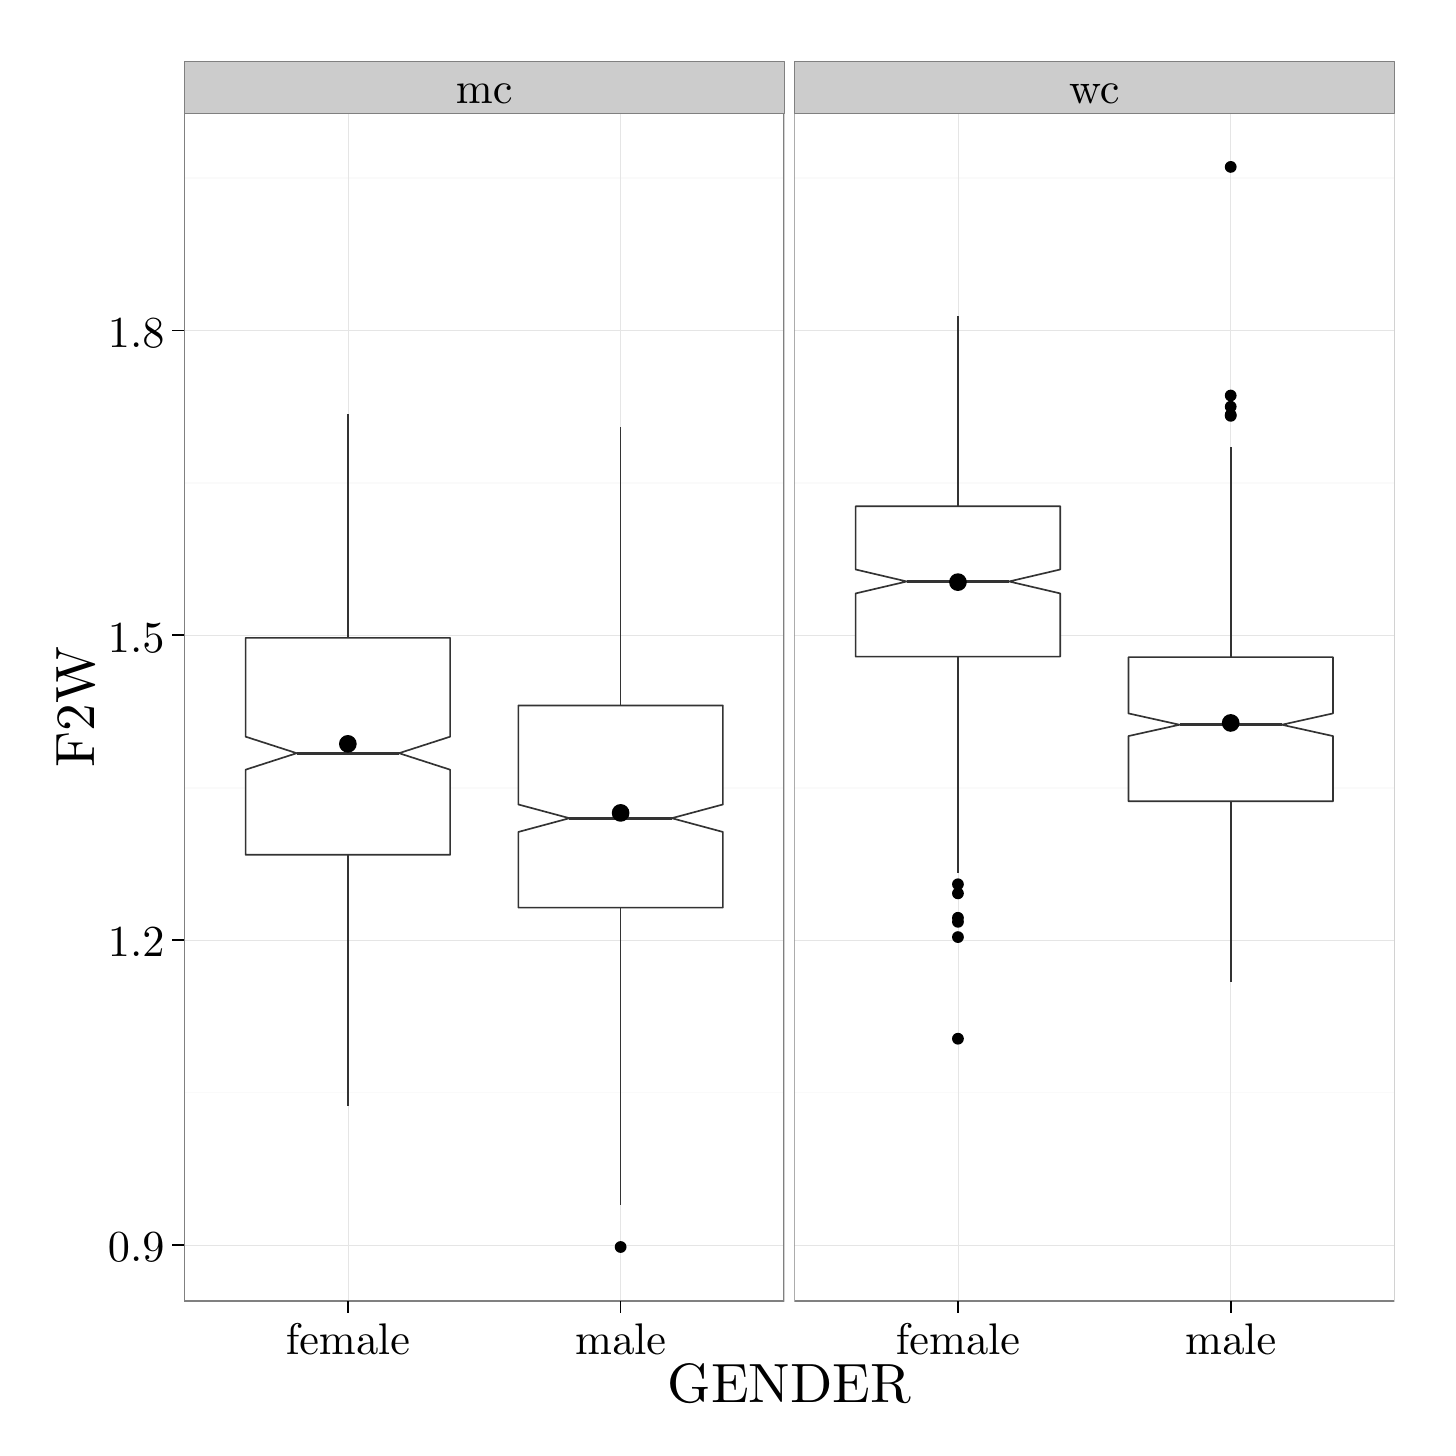
\begin{tikzpicture}[x=1pt,y=1pt]
\definecolor{fillColor}{RGB}{255,255,255}
\path[use as bounding box,fill=fillColor,fill opacity=0.00] (0,0) rectangle (505.89,505.89);
\begin{scope}
\path[clip] (  0.00,  0.00) rectangle (505.89,505.89);
\definecolor{drawColor}{RGB}{255,255,255}
\definecolor{fillColor}{RGB}{255,255,255}

\path[draw=drawColor,line width= 0.6pt,line join=round,line cap=round,fill=fillColor] (  0.00, -0.00) rectangle (505.89,505.89);
\end{scope}
\begin{scope}
\path[clip] ( 56.56, 45.77) rectangle (273.40,475.09);
\definecolor{fillColor}{RGB}{255,255,255}

\path[fill=fillColor] ( 56.56, 45.77) rectangle (273.40,475.09);
\definecolor{drawColor}{gray}{0.98}

\path[draw=drawColor,line width= 0.6pt,line join=round] ( 56.56,121.09) --
	(273.40,121.09);

\path[draw=drawColor,line width= 0.6pt,line join=round] ( 56.56,231.24) --
	(273.40,231.24);

\path[draw=drawColor,line width= 0.6pt,line join=round] ( 56.56,341.39) --
	(273.40,341.39);

\path[draw=drawColor,line width= 0.6pt,line join=round] ( 56.56,451.53) --
	(273.40,451.53);
\definecolor{drawColor}{gray}{0.90}

\path[draw=drawColor,line width= 0.2pt,line join=round] ( 56.56, 66.02) --
	(273.40, 66.02);

\path[draw=drawColor,line width= 0.2pt,line join=round] ( 56.56,176.17) --
	(273.40,176.17);

\path[draw=drawColor,line width= 0.2pt,line join=round] ( 56.56,286.31) --
	(273.40,286.31);

\path[draw=drawColor,line width= 0.2pt,line join=round] ( 56.56,396.46) --
	(273.40,396.46);

\path[draw=drawColor,line width= 0.2pt,line join=round] (115.70, 45.77) --
	(115.70,475.09);

\path[draw=drawColor,line width= 0.2pt,line join=round] (214.26, 45.77) --
	(214.26,475.09);
\definecolor{drawColor}{gray}{0.20}

\path[draw=drawColor,line width= 0.6pt,line join=round] (115.70,285.40) -- (115.70,366.35);

\path[draw=drawColor,line width= 0.6pt,line join=round] (115.70,207.01) -- (115.70,116.32);

\path[draw=drawColor,line width= 0.6pt,line join=round,line cap=round,fill=fillColor] ( 78.74,285.40) --
	( 78.74,249.69) --
	( 97.22,243.72) --
	( 78.74,237.76) --
	( 78.74,207.01) --
	(152.66,207.01) --
	(152.66,237.76) --
	(134.18,243.72) --
	(152.66,249.69) --
	(152.66,285.40) --
	( 78.74,285.40) --
	cycle;

\path[draw=drawColor,line width= 1.1pt,line join=round] ( 97.22,243.72) -- (134.18,243.72);
\definecolor{fillColor}{RGB}{0,0,0}

\path[fill=fillColor] (214.26, 65.29) circle (  2.13);

\path[draw=drawColor,line width= 0.6pt,line join=round] (214.26,260.98) -- (214.26,361.58);

\path[draw=drawColor,line width= 0.6pt,line join=round] (214.26,187.92) -- (214.26, 80.34);
\definecolor{fillColor}{RGB}{255,255,255}

\path[draw=drawColor,line width= 0.6pt,line join=round,line cap=round,fill=fillColor] (177.30,260.98) --
	(177.30,225.19) --
	(195.78,220.23) --
	(177.30,215.26) --
	(177.30,187.92) --
	(251.22,187.92) --
	(251.22,215.26) --
	(232.74,220.23) --
	(251.22,225.19) --
	(251.22,260.98) --
	(177.30,260.98) --
	cycle;

\path[draw=drawColor,line width= 1.1pt,line join=round] (195.78,220.23) -- (232.74,220.23);
\definecolor{fillColor}{RGB}{0,0,0}

\path[fill=fillColor] (115.70,247.09) circle (  3.20);

\path[fill=fillColor] (214.26,222.15) circle (  3.20);
\definecolor{drawColor}{gray}{0.50}

\path[draw=drawColor,line width= 0.6pt,line join=round,line cap=round] ( 56.56, 45.77) rectangle (273.40,475.09);
\end{scope}
\begin{scope}
\path[clip] (277.01, 45.77) rectangle (493.85,475.09);
\definecolor{fillColor}{RGB}{255,255,255}

\path[fill=fillColor] (277.01, 45.77) rectangle (493.85,475.09);
\definecolor{drawColor}{gray}{0.98}

\path[draw=drawColor,line width= 0.6pt,line join=round] (277.01,121.09) --
	(493.85,121.09);

\path[draw=drawColor,line width= 0.6pt,line join=round] (277.01,231.24) --
	(493.85,231.24);

\path[draw=drawColor,line width= 0.6pt,line join=round] (277.01,341.39) --
	(493.85,341.39);

\path[draw=drawColor,line width= 0.6pt,line join=round] (277.01,451.53) --
	(493.85,451.53);
\definecolor{drawColor}{gray}{0.90}

\path[draw=drawColor,line width= 0.2pt,line join=round] (277.01, 66.02) --
	(493.85, 66.02);

\path[draw=drawColor,line width= 0.2pt,line join=round] (277.01,176.17) --
	(493.85,176.17);

\path[draw=drawColor,line width= 0.2pt,line join=round] (277.01,286.31) --
	(493.85,286.31);

\path[draw=drawColor,line width= 0.2pt,line join=round] (277.01,396.46) --
	(493.85,396.46);

\path[draw=drawColor,line width= 0.2pt,line join=round] (336.15, 45.77) --
	(336.15,475.09);

\path[draw=drawColor,line width= 0.2pt,line join=round] (434.71, 45.77) --
	(434.71,475.09);
\definecolor{fillColor}{RGB}{0,0,0}

\path[fill=fillColor] (336.15,177.27) circle (  2.13);

\path[fill=fillColor] (336.15,196.36) circle (  2.13);

\path[fill=fillColor] (336.15,193.06) circle (  2.13);

\path[fill=fillColor] (336.15,184.24) circle (  2.13);

\path[fill=fillColor] (336.15,140.55) circle (  2.13);

\path[fill=fillColor] (336.15,182.78) circle (  2.13);
\definecolor{drawColor}{gray}{0.20}

\path[draw=drawColor,line width= 0.6pt,line join=round] (336.15,332.94) -- (336.15,401.60);

\path[draw=drawColor,line width= 0.6pt,line join=round] (336.15,278.60) -- (336.15,200.40);
\definecolor{fillColor}{RGB}{255,255,255}

\path[draw=drawColor,line width= 0.6pt,line join=round,line cap=round,fill=fillColor] (299.19,332.94) --
	(299.19,310.10) --
	(317.67,305.77) --
	(299.19,301.45) --
	(299.19,278.60) --
	(373.11,278.60) --
	(373.11,301.45) --
	(354.63,305.77) --
	(373.11,310.10) --
	(373.11,332.94) --
	(299.19,332.94) --
	cycle;

\path[draw=drawColor,line width= 1.1pt,line join=round] (317.67,305.77) -- (354.63,305.77);
\definecolor{fillColor}{RGB}{0,0,0}

\path[fill=fillColor] (434.71,365.62) circle (  2.13);

\path[fill=fillColor] (434.71,372.96) circle (  2.13);

\path[fill=fillColor] (434.71,455.57) circle (  2.13);

\path[fill=fillColor] (434.71,365.99) circle (  2.13);

\path[fill=fillColor] (434.71,368.92) circle (  2.13);

\path[draw=drawColor,line width= 0.6pt,line join=round] (434.71,278.42) -- (434.71,354.24);

\path[draw=drawColor,line width= 0.6pt,line join=round] (434.71,226.38) -- (434.71,161.11);
\definecolor{fillColor}{RGB}{255,255,255}

\path[draw=drawColor,line width= 0.6pt,line join=round,line cap=round,fill=fillColor] (397.75,278.42) --
	(397.75,258.10) --
	(416.23,254.00) --
	(397.75,249.91) --
	(397.75,226.38) --
	(471.67,226.38) --
	(471.67,249.91) --
	(453.19,254.00) --
	(471.67,258.10) --
	(471.67,278.42) --
	(397.75,278.42) --
	cycle;

\path[draw=drawColor,line width= 1.1pt,line join=round] (416.23,254.00) -- (453.19,254.00);
\definecolor{fillColor}{RGB}{0,0,0}

\path[fill=fillColor] (336.15,305.53) circle (  3.20);

\path[fill=fillColor] (434.71,254.65) circle (  3.20);
\definecolor{drawColor}{gray}{0.50}

\path[draw=drawColor,line width= 0.6pt,line join=round,line cap=round] (277.01, 45.77) rectangle (493.85,475.09);
\end{scope}
\begin{scope}
\path[clip] (  0.00,  0.00) rectangle (505.89,505.89);
\definecolor{drawColor}{gray}{0.50}
\definecolor{fillColor}{gray}{0.80}

\path[draw=drawColor,line width= 0.2pt,line join=round,line cap=round,fill=fillColor] ( 56.56,475.09) rectangle (273.40,493.85);
\definecolor{drawColor}{RGB}{0,0,0}

\node[text=drawColor,anchor=base,inner sep=0pt, outer sep=0pt, scale=  1.60] at (164.98,478.43) {mc};
\end{scope}
\begin{scope}
\path[clip] (  0.00,  0.00) rectangle (505.89,505.89);
\definecolor{drawColor}{gray}{0.50}
\definecolor{fillColor}{gray}{0.80}

\path[draw=drawColor,line width= 0.2pt,line join=round,line cap=round,fill=fillColor] (277.01,475.09) rectangle (493.85,493.85);
\definecolor{drawColor}{RGB}{0,0,0}

\node[text=drawColor,anchor=base,inner sep=0pt, outer sep=0pt, scale=  1.60] at (385.43,478.43) {wc};
\end{scope}
\begin{scope}
\path[clip] (  0.00,  0.00) rectangle (505.89,505.89);
\definecolor{drawColor}{RGB}{0,0,0}

\node[text=drawColor,anchor=base east,inner sep=0pt, outer sep=0pt, scale=  1.60] at ( 49.45, 59.99) {0.9};

\node[text=drawColor,anchor=base east,inner sep=0pt, outer sep=0pt, scale=  1.60] at ( 49.45,170.13) {1.2};

\node[text=drawColor,anchor=base east,inner sep=0pt, outer sep=0pt, scale=  1.60] at ( 49.45,280.28) {1.5};

\node[text=drawColor,anchor=base east,inner sep=0pt, outer sep=0pt, scale=  1.60] at ( 49.45,390.43) {1.8};
\end{scope}
\begin{scope}
\path[clip] (  0.00,  0.00) rectangle (505.89,505.89);
\definecolor{drawColor}{RGB}{0,0,0}

\path[draw=drawColor,line width= 0.6pt,line join=round] ( 52.30, 66.02) --
	( 56.56, 66.02);

\path[draw=drawColor,line width= 0.6pt,line join=round] ( 52.30,176.17) --
	( 56.56,176.17);

\path[draw=drawColor,line width= 0.6pt,line join=round] ( 52.30,286.31) --
	( 56.56,286.31);

\path[draw=drawColor,line width= 0.6pt,line join=round] ( 52.30,396.46) --
	( 56.56,396.46);
\end{scope}
\begin{scope}
\path[clip] (  0.00,  0.00) rectangle (505.89,505.89);
\definecolor{drawColor}{RGB}{0,0,0}

\path[draw=drawColor,line width= 0.6pt,line join=round] (115.70, 41.50) --
	(115.70, 45.77);

\path[draw=drawColor,line width= 0.6pt,line join=round] (214.26, 41.50) --
	(214.26, 45.77);
\end{scope}
\begin{scope}
\path[clip] (  0.00,  0.00) rectangle (505.89,505.89);
\definecolor{drawColor}{RGB}{0,0,0}

\node[text=drawColor,anchor=base,inner sep=0pt, outer sep=0pt, scale=  1.60] at (115.70, 26.59) {female};

\node[text=drawColor,anchor=base,inner sep=0pt, outer sep=0pt, scale=  1.60] at (214.26, 26.59) {male};
\end{scope}
\begin{scope}
\path[clip] (  0.00,  0.00) rectangle (505.89,505.89);
\definecolor{drawColor}{RGB}{0,0,0}

\path[draw=drawColor,line width= 0.6pt,line join=round] (336.15, 41.50) --
	(336.15, 45.77);

\path[draw=drawColor,line width= 0.6pt,line join=round] (434.71, 41.50) --
	(434.71, 45.77);
\end{scope}
\begin{scope}
\path[clip] (  0.00,  0.00) rectangle (505.89,505.89);
\definecolor{drawColor}{RGB}{0,0,0}

\node[text=drawColor,anchor=base,inner sep=0pt, outer sep=0pt, scale=  1.60] at (336.15, 26.59) {female};

\node[text=drawColor,anchor=base,inner sep=0pt, outer sep=0pt, scale=  1.60] at (434.71, 26.59) {male};
\end{scope}
\begin{scope}
\path[clip] (  0.00,  0.00) rectangle (505.89,505.89);
\definecolor{drawColor}{RGB}{0,0,0}

\node[text=drawColor,anchor=base,inner sep=0pt, outer sep=0pt, scale=  2.00] at (275.20,  9.03) {GENDER};
\end{scope}
\begin{scope}
\path[clip] (  0.00,  0.00) rectangle (505.89,505.89);
\definecolor{drawColor}{RGB}{0,0,0}

\node[text=drawColor,rotate= 90.00,anchor=base,inner sep=0pt, outer sep=0pt, scale=  2.00] at ( 24.12,260.43) {F2W};
\end{scope}
\end{tikzpicture}
} 
		\caption{box plot}
		\label{fig.box.f2w.nurse.genderclass}
	\end{subfigure}
	\begin{subfigure}{.49\textwidth}
		\centering
			\definecolor{shadecolor}{rgb}{0.969, 0.969, 0.969}
			\resizebox{\linewidth}{!}{% Created by tikzDevice version 0.8.1 on 2016-02-09 02:14:58
% !TEX encoding = UTF-8 Unicode
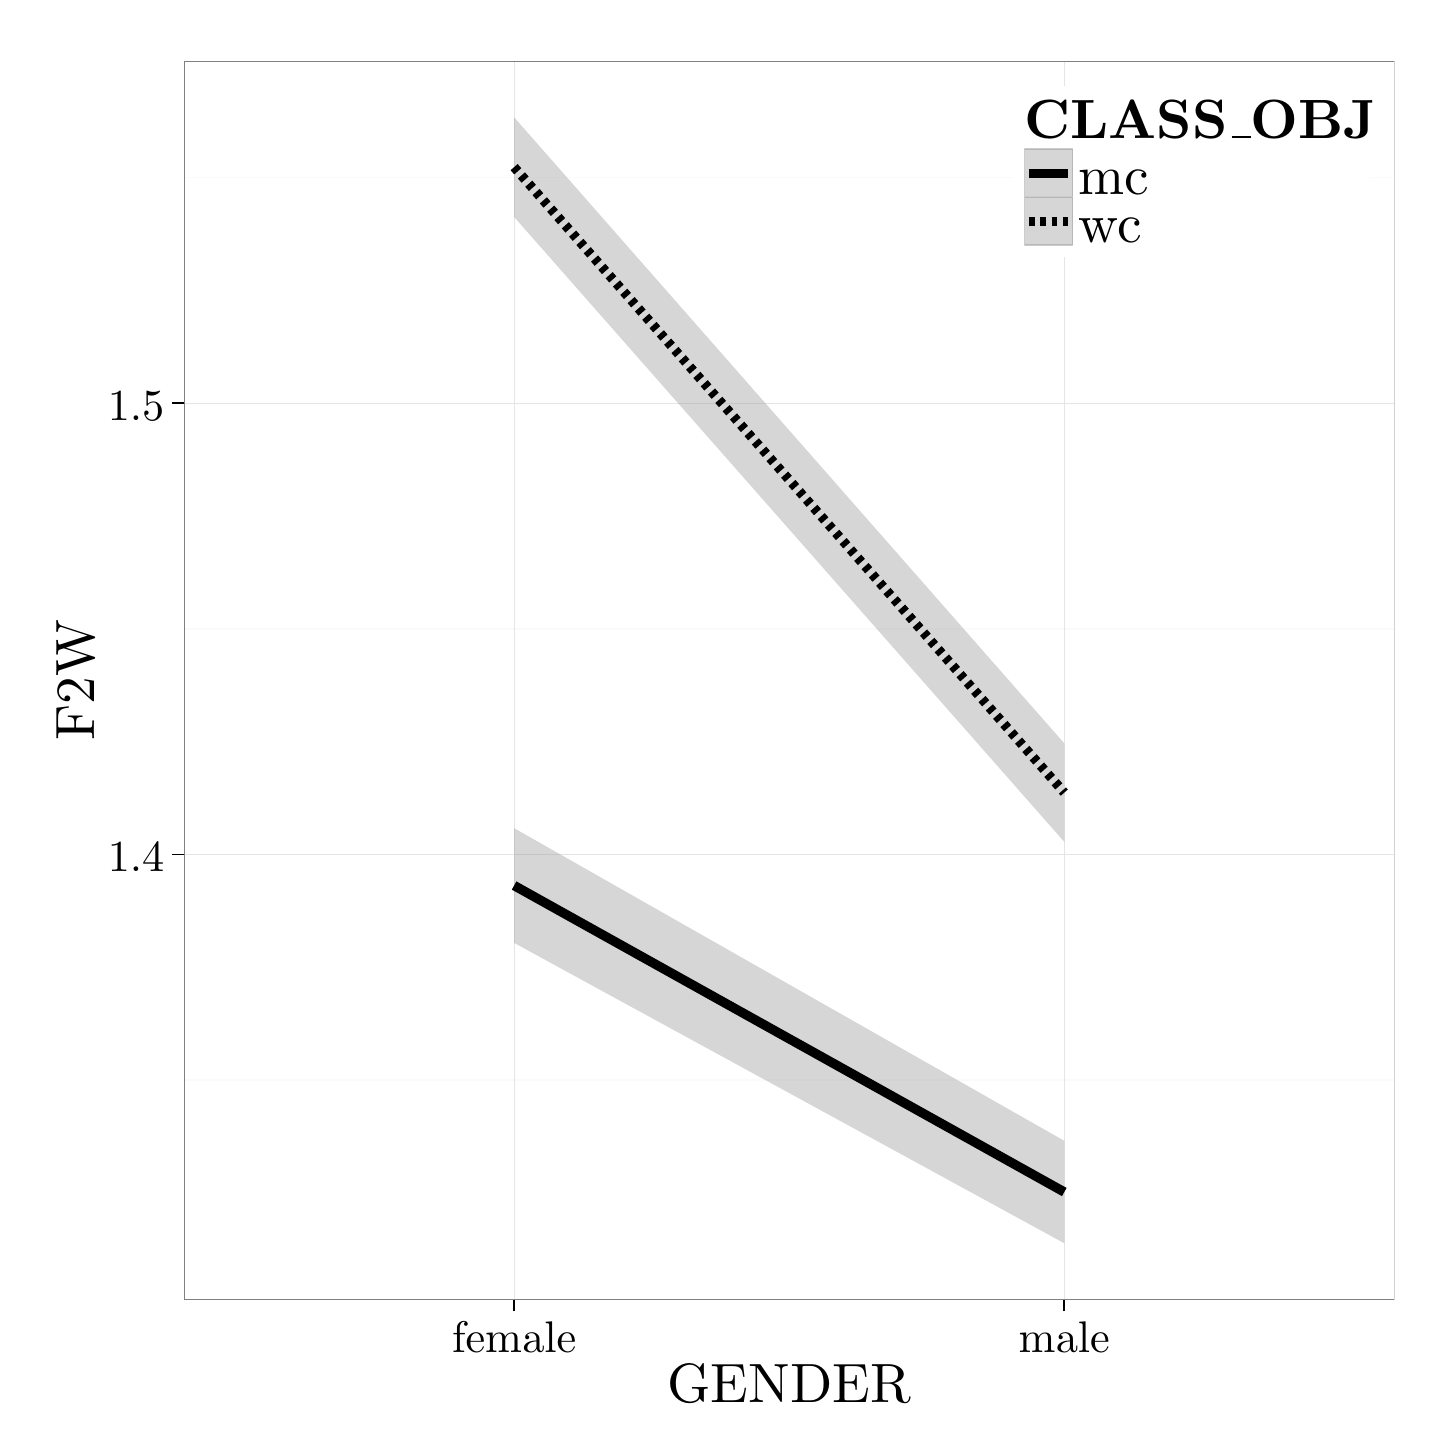
\begin{tikzpicture}[x=1pt,y=1pt]
\definecolor{fillColor}{RGB}{255,255,255}
\path[use as bounding box,fill=fillColor,fill opacity=0.00] (0,0) rectangle (505.89,505.89);
\begin{scope}
\path[clip] (  0.00,  0.00) rectangle (505.89,505.89);
\definecolor{drawColor}{RGB}{255,255,255}
\definecolor{fillColor}{RGB}{255,255,255}

\path[draw=drawColor,line width= 0.6pt,line join=round,line cap=round,fill=fillColor] (  0.00, -0.00) rectangle (505.89,505.89);
\end{scope}
\begin{scope}
\path[clip] ( 56.50, 46.31) rectangle (493.85,493.84);
\definecolor{fillColor}{RGB}{255,255,255}

\path[fill=fillColor] ( 56.50, 46.31) rectangle (493.85,493.84);
\definecolor{drawColor}{gray}{0.98}

\path[draw=drawColor,line width= 0.6pt,line join=round] ( 56.50,125.52) --
	(493.85,125.52);

\path[draw=drawColor,line width= 0.6pt,line join=round] ( 56.50,288.60) --
	(493.85,288.60);

\path[draw=drawColor,line width= 0.6pt,line join=round] ( 56.50,451.69) --
	(493.85,451.69);
\definecolor{drawColor}{gray}{0.90}

\path[draw=drawColor,line width= 0.2pt,line join=round] ( 56.50,207.06) --
	(493.85,207.06);

\path[draw=drawColor,line width= 0.2pt,line join=round] ( 56.50,370.15) --
	(493.85,370.15);

\path[draw=drawColor,line width= 0.2pt,line join=round] (175.78, 46.31) --
	(175.78,493.84);

\path[draw=drawColor,line width= 0.2pt,line join=round] (374.57, 46.31) --
	(374.57,493.84);
\definecolor{fillColor}{RGB}{153,153,153}

\path[fill=fillColor,fill opacity=0.40] (175.78,216.62) --
	(374.57,103.65) --
	(374.57, 66.65) --
	(175.78,175.17) --
	cycle;
\definecolor{drawColor}{RGB}{0,0,0}

\path[draw=drawColor,line width= 3.4pt,line join=round] (175.78,195.90) --
	(374.57, 85.15);

\path[fill=fillColor,fill opacity=0.40] (175.78,473.50) --
	(374.57,247.27) --
	(374.57,211.69) --
	(175.78,437.48) --
	cycle;

\path[draw=drawColor,line width= 3.4pt,dash pattern=on 2pt off 2pt ,line join=round] (175.78,455.49) --
	(374.57,229.48);
\definecolor{drawColor}{gray}{0.50}

\path[draw=drawColor,line width= 0.6pt,line join=round,line cap=round] ( 56.50, 46.31) rectangle (493.85,493.84);
\end{scope}
\begin{scope}
\path[clip] (  0.00,  0.00) rectangle (505.89,505.89);
\definecolor{drawColor}{RGB}{0,0,0}

\node[text=drawColor,anchor=base east,inner sep=0pt, outer sep=0pt, scale=  1.60] at ( 49.39,201.03) {1.4};

\node[text=drawColor,anchor=base east,inner sep=0pt, outer sep=0pt, scale=  1.60] at ( 49.39,364.11) {1.5};
\end{scope}
\begin{scope}
\path[clip] (  0.00,  0.00) rectangle (505.89,505.89);
\definecolor{drawColor}{RGB}{0,0,0}

\path[draw=drawColor,line width= 0.6pt,line join=round] ( 52.24,207.06) --
	( 56.50,207.06);

\path[draw=drawColor,line width= 0.6pt,line join=round] ( 52.24,370.15) --
	( 56.50,370.15);
\end{scope}
\begin{scope}
\path[clip] (  0.00,  0.00) rectangle (505.89,505.89);
\definecolor{drawColor}{RGB}{0,0,0}

\path[draw=drawColor,line width= 0.6pt,line join=round] (175.78, 42.04) --
	(175.78, 46.31);

\path[draw=drawColor,line width= 0.6pt,line join=round] (374.57, 42.04) --
	(374.57, 46.31);
\end{scope}
\begin{scope}
\path[clip] (  0.00,  0.00) rectangle (505.89,505.89);
\definecolor{drawColor}{RGB}{0,0,0}

\node[text=drawColor,anchor=base,inner sep=0pt, outer sep=0pt, scale=  1.60] at (175.78, 27.13) {female};

\node[text=drawColor,anchor=base,inner sep=0pt, outer sep=0pt, scale=  1.60] at (374.57, 27.13) {male};
\end{scope}
\begin{scope}
\path[clip] (  0.00,  0.00) rectangle (505.89,505.89);
\definecolor{drawColor}{RGB}{0,0,0}

\node[text=drawColor,anchor=base,inner sep=0pt, outer sep=0pt, scale=  2.00] at (275.17,  9.03) {GENDER};
\end{scope}
\begin{scope}
\path[clip] (  0.00,  0.00) rectangle (505.89,505.89);
\definecolor{drawColor}{RGB}{0,0,0}

\node[text=drawColor,rotate= 90.00,anchor=base,inner sep=0pt, outer sep=0pt, scale=  2.00] at ( 24.12,270.08) {F2W};
\end{scope}
\begin{scope}
\path[clip] (  0.00,  0.00) rectangle (505.89,505.89);
\definecolor{fillColor}{RGB}{255,255,255}

\path[fill=fillColor] (355.97,423.00) rectangle (484.98,484.98);
\end{scope}
\begin{scope}
\path[clip] (  0.00,  0.00) rectangle (505.89,505.89);
\definecolor{drawColor}{RGB}{0,0,0}

\node[text=drawColor,anchor=base west,inner sep=0pt, outer sep=0pt, scale=  2.00] at (360.24,465.96) {\bfseries CLASS{\_{}}OBJ};
\end{scope}
\begin{scope}
\path[clip] (  0.00,  0.00) rectangle (505.89,505.89);
\definecolor{drawColor}{gray}{0.80}
\definecolor{fillColor}{RGB}{255,255,255}

\path[draw=drawColor,line width= 0.6pt,line join=round,line cap=round,fill=fillColor] (360.24,444.61) rectangle (377.58,461.96);
\end{scope}
\begin{scope}
\path[clip] (  0.00,  0.00) rectangle (505.89,505.89);
\definecolor{fillColor}{RGB}{153,153,153}

\path[fill=fillColor,fill opacity=0.40] (360.24,444.61) rectangle (377.58,461.96);
\definecolor{drawColor}{RGB}{0,0,0}

\path[draw=drawColor,line width= 3.4pt,line join=round] (361.97,453.29) -- (375.85,453.29);
\end{scope}
\begin{scope}
\path[clip] (  0.00,  0.00) rectangle (505.89,505.89);
\definecolor{drawColor}{gray}{0.80}
\definecolor{fillColor}{RGB}{255,255,255}

\path[draw=drawColor,line width= 0.6pt,line join=round,line cap=round,fill=fillColor] (360.24,427.27) rectangle (377.58,444.61);
\end{scope}
\begin{scope}
\path[clip] (  0.00,  0.00) rectangle (505.89,505.89);
\definecolor{fillColor}{RGB}{153,153,153}

\path[fill=fillColor,fill opacity=0.40] (360.24,427.27) rectangle (377.58,444.61);
\definecolor{drawColor}{RGB}{0,0,0}

\path[draw=drawColor,line width= 3.4pt,dash pattern=on 2pt off 2pt ,line join=round] (361.97,435.94) -- (375.85,435.94);
\end{scope}
\begin{scope}
\path[clip] (  0.00,  0.00) rectangle (505.89,505.89);
\definecolor{drawColor}{RGB}{0,0,0}

\node[text=drawColor,anchor=base west,inner sep=0pt, outer sep=0pt, scale=  2.00] at (379.75,445.75) {mc};
\end{scope}
\begin{scope}
\path[clip] (  0.00,  0.00) rectangle (505.89,505.89);
\definecolor{drawColor}{RGB}{0,0,0}

\node[text=drawColor,anchor=base west,inner sep=0pt, outer sep=0pt, scale=  2.00] at (379.75,428.40) {wc};
\end{scope}
\end{tikzpicture}
} 
		\caption{regression plot}
		\label{fig.scatter.f2w.nurse.genderclass}
	\end{subfigure}
	\caption{\textsc{nurse} (F2) by gender and class}
\end{figure}

The first interaction we will look at is that of gender and social class of participant, which is illustrated in Figures \ref{fig.box.f2w.nurse.genderclass} and \ref{fig.scatter.f2w.nurse.genderclass}.
The two box plots show the difference between the two genders in the middle and the working class, respectively.
Male speakers have a lower mean F2 than women in both classes.
This is a surprising result because lower F2 values mean more central realisations and more central variants of \textsc{nurse} are \emph{less} Scouse variants of \textsc{nurse}.
In most sociolinguistic studies, however, men have been found to be \emph{more} likely than women to use local variants of socially meaningful variables.
Judging from the plot, the difference between genders is already highly significant in the middle-class sample (left panel) because not only are the means of women and men clearly distinct, but they are also virtually identical to the medians of the same category (which argues for normally distributed data), and the confidence intervals do not occupy the same space at all.
A t-test confirms this interpretation (t(901.122) = 7.779, p < 0.001).
It is also obvious, however, that the difference between women and men is much more prounounced in the working class (right panel):
\begin{inparaenum}[(a)]
	\item The distance between the means is considerably greater, and
	\item even the interquartile ranges (visualised through the size and position of the boxes) hardly overlap, let alone the confidence intervals (t(791.427) = 17.513, p < 0.001).
\end{inparaenum}

The fact that gender has a more drastic effect in the working class than in the middle class is also illustrated by the regression plot in Figure \ref{fig.scatter.f2w.nurse.genderclass}, where gender is to be found on the x-, and estimated F2 on the y-axis.
A greater effect of gender should, in this graph, translate to a steeper slope of the regression line from `female' to `male', and this is precisely what we find when we compare the dotted (working class) to the solid (middle class) line.
What we can also see is that middle-class speakers have lower F2 values than their working-class counterparts (the solid line is below the dotted one).
This is not surprising because it means that middle-class speakers use less Scouse variants than working-class Liverpudlians, which is true for both female (t(815.432) = -18.076, p < 0.001) and male subjects (t(933.018) = -11.305, p < 0.001).
Social classes are less distinct when we focus on male subjects only (the vertical distance between the regression lines is smaller), but it should be noted that this is a highly relative statement as the difference is statistically extremely robust for this sub-group of speakers, too.
The significant interaction in the mixed-effects regression is thus not due to there being an effect in different directions in the sub-samples, but it is `merely' an expression of the fact that the effect of gender (class) is stronger for working-class (female) subjects.

\subsubsection{Gender and age}
\label{sec.prod.res.vow.nurse.f2.genderage}

\begin{figure}[h!]
	\centering
	\begin{subfigure}{.49\textwidth}
		\centering
			\definecolor{shadecolor}{rgb}{0.969, 0.969, 0.969}
			\resizebox{\linewidth}{!}{% Created by tikzDevice version 0.8.1 on 2016-02-09 02:15:01
% !TEX encoding = UTF-8 Unicode
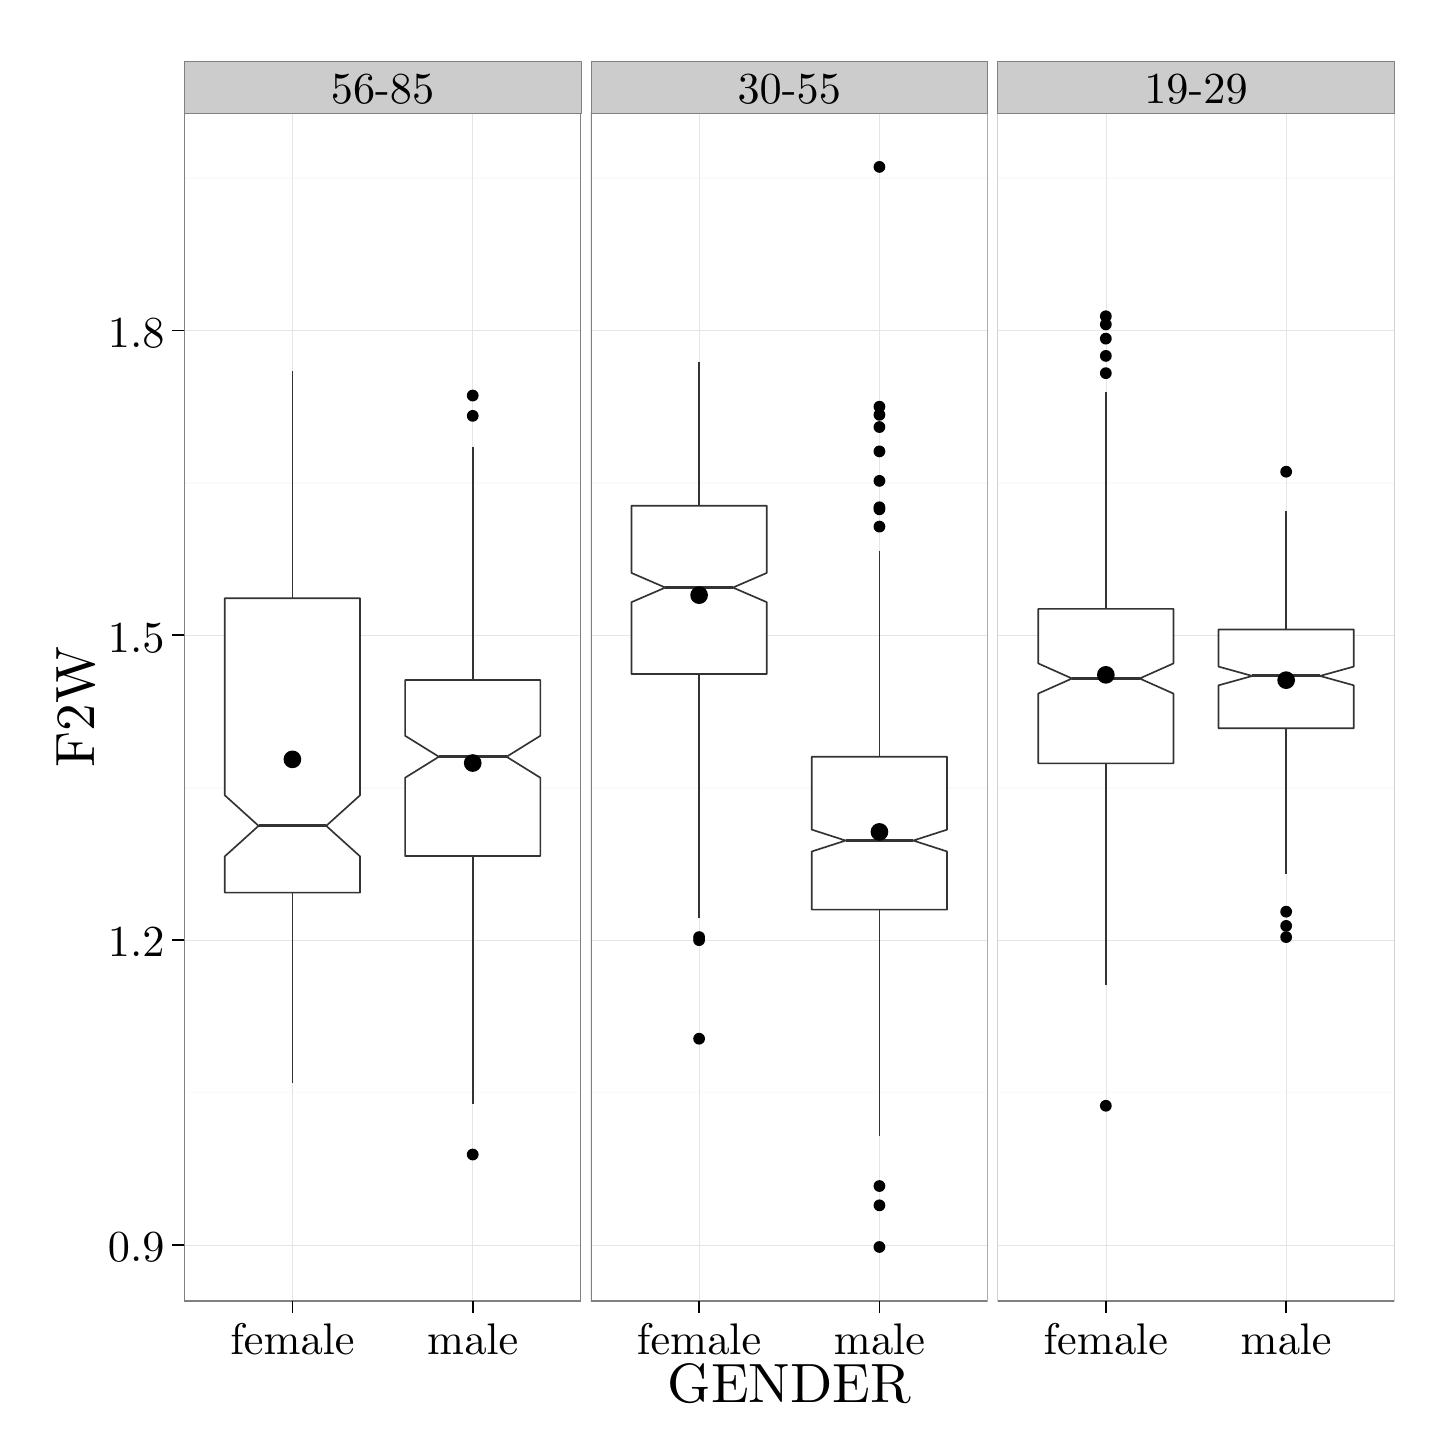
\begin{tikzpicture}[x=1pt,y=1pt]
\definecolor{fillColor}{RGB}{255,255,255}
\path[use as bounding box,fill=fillColor,fill opacity=0.00] (0,0) rectangle (505.89,505.89);
\begin{scope}
\path[clip] (  0.00,  0.00) rectangle (505.89,505.89);
\definecolor{drawColor}{RGB}{255,255,255}
\definecolor{fillColor}{RGB}{255,255,255}

\path[draw=drawColor,line width= 0.6pt,line join=round,line cap=round,fill=fillColor] (  0.00, -0.00) rectangle (505.89,505.89);
\end{scope}
\begin{scope}
\path[clip] ( 56.56, 45.77) rectangle (199.92,475.09);
\definecolor{fillColor}{RGB}{255,255,255}

\path[fill=fillColor] ( 56.56, 45.77) rectangle (199.92,475.09);
\definecolor{drawColor}{gray}{0.98}

\path[draw=drawColor,line width= 0.6pt,line join=round] ( 56.56,121.09) --
	(199.92,121.09);

\path[draw=drawColor,line width= 0.6pt,line join=round] ( 56.56,231.24) --
	(199.92,231.24);

\path[draw=drawColor,line width= 0.6pt,line join=round] ( 56.56,341.39) --
	(199.92,341.39);

\path[draw=drawColor,line width= 0.6pt,line join=round] ( 56.56,451.53) --
	(199.92,451.53);
\definecolor{drawColor}{gray}{0.90}

\path[draw=drawColor,line width= 0.2pt,line join=round] ( 56.56, 66.02) --
	(199.92, 66.02);

\path[draw=drawColor,line width= 0.2pt,line join=round] ( 56.56,176.17) --
	(199.92,176.17);

\path[draw=drawColor,line width= 0.2pt,line join=round] ( 56.56,286.31) --
	(199.92,286.31);

\path[draw=drawColor,line width= 0.2pt,line join=round] ( 56.56,396.46) --
	(199.92,396.46);

\path[draw=drawColor,line width= 0.2pt,line join=round] ( 95.66, 45.77) --
	( 95.66,475.09);

\path[draw=drawColor,line width= 0.2pt,line join=round] (160.82, 45.77) --
	(160.82,475.09);
\definecolor{drawColor}{gray}{0.20}

\path[draw=drawColor,line width= 0.6pt,line join=round] ( 95.66,299.72) -- ( 95.66,381.77);

\path[draw=drawColor,line width= 0.6pt,line join=round] ( 95.66,193.33) -- ( 95.66,124.40);

\path[draw=drawColor,line width= 0.6pt,line join=round,line cap=round,fill=fillColor] ( 71.23,299.72) --
	( 71.23,228.51) --
	( 83.44,217.47) --
	( 71.23,206.44) --
	( 71.23,193.33) --
	(120.10,193.33) --
	(120.10,206.44) --
	(107.88,217.47) --
	(120.10,228.51) --
	(120.10,299.72) --
	( 71.23,299.72) --
	cycle;

\path[draw=drawColor,line width= 1.1pt,line join=round] ( 83.44,217.47) -- (107.88,217.47);
\definecolor{fillColor}{RGB}{0,0,0}

\path[fill=fillColor] (160.82,365.62) circle (  2.13);

\path[fill=fillColor] (160.82,372.96) circle (  2.13);

\path[fill=fillColor] (160.82, 98.70) circle (  2.13);

\path[draw=drawColor,line width= 0.6pt,line join=round] (160.82,270.16) -- (160.82,354.24);

\path[draw=drawColor,line width= 0.6pt,line join=round] (160.82,206.55) -- (160.82,117.06);
\definecolor{fillColor}{RGB}{255,255,255}

\path[draw=drawColor,line width= 0.6pt,line join=round,line cap=round,fill=fillColor] (136.39,270.16) --
	(136.39,250.01) --
	(148.60,242.44) --
	(136.39,234.86) --
	(136.39,206.55) --
	(185.25,206.55) --
	(185.25,234.86) --
	(173.04,242.44) --
	(185.25,250.01) --
	(185.25,270.16) --
	(136.39,270.16) --
	cycle;

\path[draw=drawColor,line width= 1.1pt,line join=round] (148.60,242.44) -- (173.04,242.44);
\definecolor{fillColor}{RGB}{0,0,0}

\path[fill=fillColor] ( 95.66,241.49) circle (  3.20);

\path[fill=fillColor] (160.82,240.16) circle (  3.20);
\definecolor{drawColor}{gray}{0.50}

\path[draw=drawColor,line width= 0.6pt,line join=round,line cap=round] ( 56.56, 45.77) rectangle (199.92,475.09);
\end{scope}
\begin{scope}
\path[clip] (203.53, 45.77) rectangle (346.88,475.09);
\definecolor{fillColor}{RGB}{255,255,255}

\path[fill=fillColor] (203.53, 45.77) rectangle (346.88,475.09);
\definecolor{drawColor}{gray}{0.98}

\path[draw=drawColor,line width= 0.6pt,line join=round] (203.53,121.09) --
	(346.88,121.09);

\path[draw=drawColor,line width= 0.6pt,line join=round] (203.53,231.24) --
	(346.88,231.24);

\path[draw=drawColor,line width= 0.6pt,line join=round] (203.53,341.39) --
	(346.88,341.39);

\path[draw=drawColor,line width= 0.6pt,line join=round] (203.53,451.53) --
	(346.88,451.53);
\definecolor{drawColor}{gray}{0.90}

\path[draw=drawColor,line width= 0.2pt,line join=round] (203.53, 66.02) --
	(346.88, 66.02);

\path[draw=drawColor,line width= 0.2pt,line join=round] (203.53,176.17) --
	(346.88,176.17);

\path[draw=drawColor,line width= 0.2pt,line join=round] (203.53,286.31) --
	(346.88,286.31);

\path[draw=drawColor,line width= 0.2pt,line join=round] (203.53,396.46) --
	(346.88,396.46);

\path[draw=drawColor,line width= 0.2pt,line join=round] (242.62, 45.77) --
	(242.62,475.09);

\path[draw=drawColor,line width= 0.2pt,line join=round] (307.78, 45.77) --
	(307.78,475.09);
\definecolor{fillColor}{RGB}{0,0,0}

\path[fill=fillColor] (242.62,177.27) circle (  2.13);

\path[fill=fillColor] (242.62,140.55) circle (  2.13);

\path[fill=fillColor] (242.62,176.17) circle (  2.13);
\definecolor{drawColor}{gray}{0.20}

\path[draw=drawColor,line width= 0.6pt,line join=round] (242.62,333.13) -- (242.62,385.08);

\path[draw=drawColor,line width= 0.6pt,line join=round] (242.62,272.36) -- (242.62,184.24);
\definecolor{fillColor}{RGB}{255,255,255}

\path[draw=drawColor,line width= 0.6pt,line join=round,line cap=round,fill=fillColor] (218.19,333.13) --
	(218.19,308.85) --
	(230.41,303.57) --
	(218.19,298.29) --
	(218.19,272.36) --
	(267.06,272.36) --
	(267.06,298.29) --
	(254.84,303.57) --
	(267.06,308.85) --
	(267.06,333.13) --
	(218.19,333.13) --
	cycle;

\path[draw=drawColor,line width= 1.1pt,line join=round] (230.41,303.57) -- (254.84,303.57);
\definecolor{fillColor}{RGB}{0,0,0}

\path[fill=fillColor] (307.78,325.60) circle (  2.13);

\path[fill=fillColor] (307.78, 65.29) circle (  2.13);

\path[fill=fillColor] (307.78, 80.34) circle (  2.13);

\path[fill=fillColor] (307.78, 87.32) circle (  2.13);

\path[fill=fillColor] (307.78,361.58) circle (  2.13);

\path[fill=fillColor] (307.78,455.57) circle (  2.13);

\path[fill=fillColor] (307.78,352.77) circle (  2.13);

\path[fill=fillColor] (307.78,342.12) circle (  2.13);

\path[fill=fillColor] (307.78,365.99) circle (  2.13);

\path[fill=fillColor] (307.78,332.58) circle (  2.13);

\path[fill=fillColor] (307.78,331.84) circle (  2.13);

\path[fill=fillColor] (307.78,368.92) circle (  2.13);

\path[draw=drawColor,line width= 0.6pt,line join=round] (307.78,242.44) -- (307.78,316.79);

\path[draw=drawColor,line width= 0.6pt,line join=round] (307.78,187.18) -- (307.78,105.31);
\definecolor{fillColor}{RGB}{255,255,255}

\path[draw=drawColor,line width= 0.6pt,line join=round,line cap=round,fill=fillColor] (283.35,242.44) --
	(283.35,216.09) --
	(295.57,212.15) --
	(283.35,208.21) --
	(283.35,187.18) --
	(332.22,187.18) --
	(332.22,208.21) --
	(320.00,212.15) --
	(332.22,216.09) --
	(332.22,242.44) --
	(283.35,242.44) --
	cycle;

\path[draw=drawColor,line width= 1.1pt,line join=round] (295.57,212.15) -- (320.00,212.15);
\definecolor{fillColor}{RGB}{0,0,0}

\path[fill=fillColor] (242.62,300.83) circle (  3.20);

\path[fill=fillColor] (307.78,215.28) circle (  3.20);
\definecolor{drawColor}{gray}{0.50}

\path[draw=drawColor,line width= 0.6pt,line join=round,line cap=round] (203.53, 45.77) rectangle (346.88,475.09);
\end{scope}
\begin{scope}
\path[clip] (350.49, 45.77) rectangle (493.85,475.09);
\definecolor{fillColor}{RGB}{255,255,255}

\path[fill=fillColor] (350.49, 45.77) rectangle (493.85,475.09);
\definecolor{drawColor}{gray}{0.98}

\path[draw=drawColor,line width= 0.6pt,line join=round] (350.49,121.09) --
	(493.85,121.09);

\path[draw=drawColor,line width= 0.6pt,line join=round] (350.49,231.24) --
	(493.85,231.24);

\path[draw=drawColor,line width= 0.6pt,line join=round] (350.49,341.39) --
	(493.85,341.39);

\path[draw=drawColor,line width= 0.6pt,line join=round] (350.49,451.53) --
	(493.85,451.53);
\definecolor{drawColor}{gray}{0.90}

\path[draw=drawColor,line width= 0.2pt,line join=round] (350.49, 66.02) --
	(493.85, 66.02);

\path[draw=drawColor,line width= 0.2pt,line join=round] (350.49,176.17) --
	(493.85,176.17);

\path[draw=drawColor,line width= 0.2pt,line join=round] (350.49,286.31) --
	(493.85,286.31);

\path[draw=drawColor,line width= 0.2pt,line join=round] (350.49,396.46) --
	(493.85,396.46);

\path[draw=drawColor,line width= 0.2pt,line join=round] (389.59, 45.77) --
	(389.59,475.09);

\path[draw=drawColor,line width= 0.2pt,line join=round] (454.75, 45.77) --
	(454.75,475.09);
\definecolor{fillColor}{RGB}{0,0,0}

\path[fill=fillColor] (389.59,116.32) circle (  2.13);

\path[fill=fillColor] (389.59,401.60) circle (  2.13);

\path[fill=fillColor] (389.59,387.28) circle (  2.13);

\path[fill=fillColor] (389.59,381.04) circle (  2.13);

\path[fill=fillColor] (389.59,393.52) circle (  2.13);

\path[fill=fillColor] (389.59,398.66) circle (  2.13);
\definecolor{drawColor}{gray}{0.20}

\path[draw=drawColor,line width= 0.6pt,line join=round] (389.59,295.86) -- (389.59,374.06);

\path[draw=drawColor,line width= 0.6pt,line join=round] (389.59,240.05) -- (389.59,160.01);
\definecolor{fillColor}{RGB}{255,255,255}

\path[draw=drawColor,line width= 0.6pt,line join=round,line cap=round,fill=fillColor] (365.15,295.86) --
	(365.15,276.16) --
	(377.37,270.71) --
	(365.15,265.26) --
	(365.15,240.05) --
	(414.02,240.05) --
	(414.02,265.26) --
	(401.81,270.71) --
	(414.02,276.16) --
	(414.02,295.86) --
	(365.15,295.86) --
	cycle;

\path[draw=drawColor,line width= 1.1pt,line join=round] (377.37,270.71) -- (401.81,270.71);
\definecolor{fillColor}{RGB}{0,0,0}

\path[fill=fillColor] (454.75,181.31) circle (  2.13);

\path[fill=fillColor] (454.75,177.27) circle (  2.13);

\path[fill=fillColor] (454.75,345.43) circle (  2.13);

\path[fill=fillColor] (454.75,186.45) circle (  2.13);

\path[draw=drawColor,line width= 0.6pt,line join=round] (454.75,288.43) -- (454.75,331.11);

\path[draw=drawColor,line width= 0.6pt,line join=round] (454.75,252.72) -- (454.75,200.03);
\definecolor{fillColor}{RGB}{255,255,255}

\path[draw=drawColor,line width= 0.6pt,line join=round,line cap=round,fill=fillColor] (430.31,288.43) --
	(430.31,275.01) --
	(442.53,271.63) --
	(430.31,268.24) --
	(430.31,252.72) --
	(479.18,252.72) --
	(479.18,268.24) --
	(466.97,271.63) --
	(479.18,275.01) --
	(479.18,288.43) --
	(430.31,288.43) --
	cycle;

\path[draw=drawColor,line width= 1.1pt,line join=round] (442.53,271.63) -- (466.97,271.63);
\definecolor{fillColor}{RGB}{0,0,0}

\path[fill=fillColor] (389.59,272.03) circle (  3.20);

\path[fill=fillColor] (454.75,270.11) circle (  3.20);
\definecolor{drawColor}{gray}{0.50}

\path[draw=drawColor,line width= 0.6pt,line join=round,line cap=round] (350.49, 45.77) rectangle (493.85,475.09);
\end{scope}
\begin{scope}
\path[clip] (  0.00,  0.00) rectangle (505.89,505.89);
\definecolor{drawColor}{gray}{0.50}
\definecolor{fillColor}{gray}{0.80}

\path[draw=drawColor,line width= 0.2pt,line join=round,line cap=round,fill=fillColor] ( 56.56,475.09) rectangle (199.92,493.85);
\definecolor{drawColor}{RGB}{0,0,0}

\node[text=drawColor,anchor=base,inner sep=0pt, outer sep=0pt, scale=  1.60] at (128.24,478.43) {56-85};
\end{scope}
\begin{scope}
\path[clip] (  0.00,  0.00) rectangle (505.89,505.89);
\definecolor{drawColor}{gray}{0.50}
\definecolor{fillColor}{gray}{0.80}

\path[draw=drawColor,line width= 0.2pt,line join=round,line cap=round,fill=fillColor] (203.53,475.09) rectangle (346.88,493.85);
\definecolor{drawColor}{RGB}{0,0,0}

\node[text=drawColor,anchor=base,inner sep=0pt, outer sep=0pt, scale=  1.60] at (275.20,478.43) {30-55};
\end{scope}
\begin{scope}
\path[clip] (  0.00,  0.00) rectangle (505.89,505.89);
\definecolor{drawColor}{gray}{0.50}
\definecolor{fillColor}{gray}{0.80}

\path[draw=drawColor,line width= 0.2pt,line join=round,line cap=round,fill=fillColor] (350.49,475.09) rectangle (493.85,493.85);
\definecolor{drawColor}{RGB}{0,0,0}

\node[text=drawColor,anchor=base,inner sep=0pt, outer sep=0pt, scale=  1.60] at (422.17,478.43) {19-29};
\end{scope}
\begin{scope}
\path[clip] (  0.00,  0.00) rectangle (505.89,505.89);
\definecolor{drawColor}{RGB}{0,0,0}

\node[text=drawColor,anchor=base east,inner sep=0pt, outer sep=0pt, scale=  1.60] at ( 49.45, 59.99) {0.9};

\node[text=drawColor,anchor=base east,inner sep=0pt, outer sep=0pt, scale=  1.60] at ( 49.45,170.13) {1.2};

\node[text=drawColor,anchor=base east,inner sep=0pt, outer sep=0pt, scale=  1.60] at ( 49.45,280.28) {1.5};

\node[text=drawColor,anchor=base east,inner sep=0pt, outer sep=0pt, scale=  1.60] at ( 49.45,390.43) {1.8};
\end{scope}
\begin{scope}
\path[clip] (  0.00,  0.00) rectangle (505.89,505.89);
\definecolor{drawColor}{RGB}{0,0,0}

\path[draw=drawColor,line width= 0.6pt,line join=round] ( 52.30, 66.02) --
	( 56.56, 66.02);

\path[draw=drawColor,line width= 0.6pt,line join=round] ( 52.30,176.17) --
	( 56.56,176.17);

\path[draw=drawColor,line width= 0.6pt,line join=round] ( 52.30,286.31) --
	( 56.56,286.31);

\path[draw=drawColor,line width= 0.6pt,line join=round] ( 52.30,396.46) --
	( 56.56,396.46);
\end{scope}
\begin{scope}
\path[clip] (  0.00,  0.00) rectangle (505.89,505.89);
\definecolor{drawColor}{RGB}{0,0,0}

\path[draw=drawColor,line width= 0.6pt,line join=round] ( 95.66, 41.50) --
	( 95.66, 45.77);

\path[draw=drawColor,line width= 0.6pt,line join=round] (160.82, 41.50) --
	(160.82, 45.77);
\end{scope}
\begin{scope}
\path[clip] (  0.00,  0.00) rectangle (505.89,505.89);
\definecolor{drawColor}{RGB}{0,0,0}

\node[text=drawColor,anchor=base,inner sep=0pt, outer sep=0pt, scale=  1.60] at ( 95.66, 26.59) {female};

\node[text=drawColor,anchor=base,inner sep=0pt, outer sep=0pt, scale=  1.60] at (160.82, 26.59) {male};
\end{scope}
\begin{scope}
\path[clip] (  0.00,  0.00) rectangle (505.89,505.89);
\definecolor{drawColor}{RGB}{0,0,0}

\path[draw=drawColor,line width= 0.6pt,line join=round] (242.62, 41.50) --
	(242.62, 45.77);

\path[draw=drawColor,line width= 0.6pt,line join=round] (307.78, 41.50) --
	(307.78, 45.77);
\end{scope}
\begin{scope}
\path[clip] (  0.00,  0.00) rectangle (505.89,505.89);
\definecolor{drawColor}{RGB}{0,0,0}

\node[text=drawColor,anchor=base,inner sep=0pt, outer sep=0pt, scale=  1.60] at (242.62, 26.59) {female};

\node[text=drawColor,anchor=base,inner sep=0pt, outer sep=0pt, scale=  1.60] at (307.78, 26.59) {male};
\end{scope}
\begin{scope}
\path[clip] (  0.00,  0.00) rectangle (505.89,505.89);
\definecolor{drawColor}{RGB}{0,0,0}

\path[draw=drawColor,line width= 0.6pt,line join=round] (389.59, 41.50) --
	(389.59, 45.77);

\path[draw=drawColor,line width= 0.6pt,line join=round] (454.75, 41.50) --
	(454.75, 45.77);
\end{scope}
\begin{scope}
\path[clip] (  0.00,  0.00) rectangle (505.89,505.89);
\definecolor{drawColor}{RGB}{0,0,0}

\node[text=drawColor,anchor=base,inner sep=0pt, outer sep=0pt, scale=  1.60] at (389.59, 26.59) {female};

\node[text=drawColor,anchor=base,inner sep=0pt, outer sep=0pt, scale=  1.60] at (454.75, 26.59) {male};
\end{scope}
\begin{scope}
\path[clip] (  0.00,  0.00) rectangle (505.89,505.89);
\definecolor{drawColor}{RGB}{0,0,0}

\node[text=drawColor,anchor=base,inner sep=0pt, outer sep=0pt, scale=  2.00] at (275.20,  9.03) {GENDER};
\end{scope}
\begin{scope}
\path[clip] (  0.00,  0.00) rectangle (505.89,505.89);
\definecolor{drawColor}{RGB}{0,0,0}

\node[text=drawColor,rotate= 90.00,anchor=base,inner sep=0pt, outer sep=0pt, scale=  2.00] at ( 24.12,260.43) {F2W};
\end{scope}
\end{tikzpicture}
} 
		\caption{box plot}
		\label{fig.box.f2w.nurse.genderage}
	\end{subfigure}
	\begin{subfigure}{.49\textwidth}
		\centering
			\definecolor{shadecolor}{rgb}{0.969, 0.969, 0.969}
			\resizebox{\linewidth}{!}{% Created by tikzDevice version 0.8.1 on 2016-02-09 02:15:01
% !TEX encoding = UTF-8 Unicode
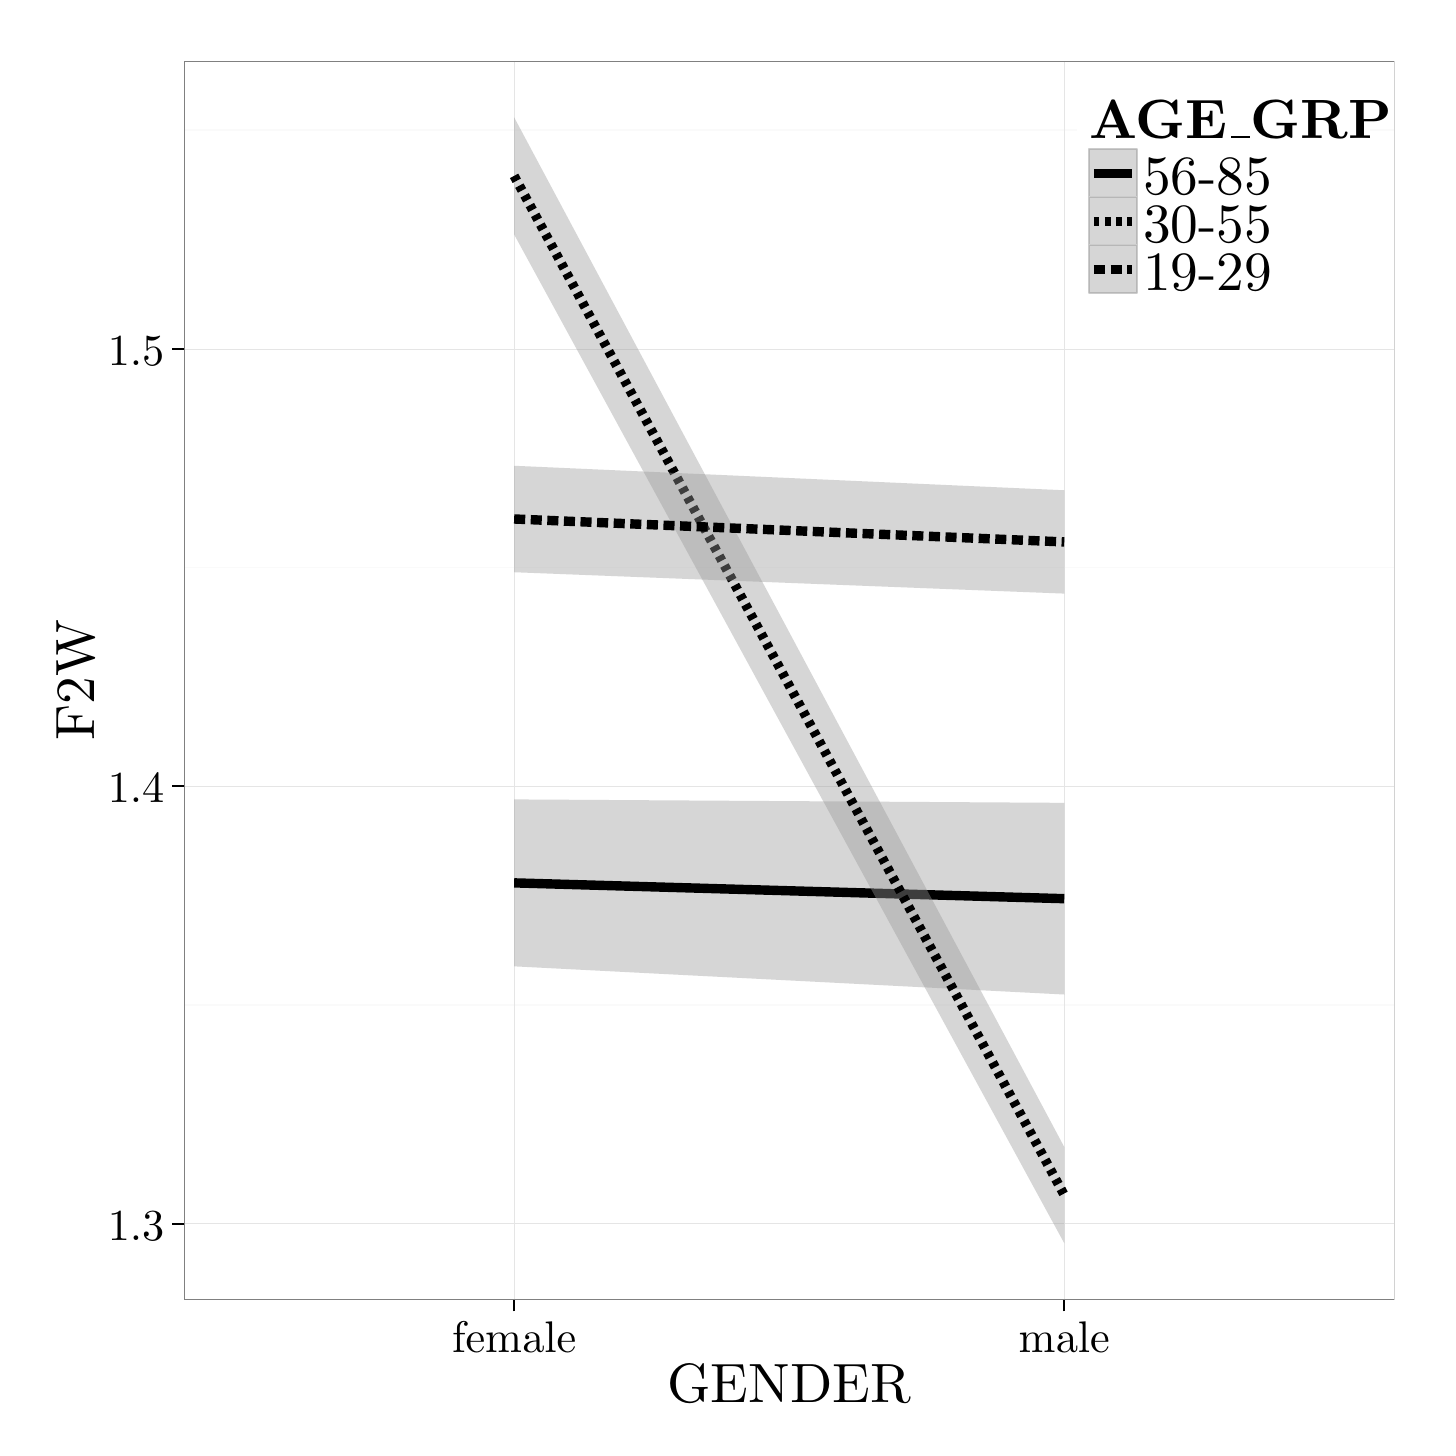
\begin{tikzpicture}[x=1pt,y=1pt]
\definecolor{fillColor}{RGB}{255,255,255}
\path[use as bounding box,fill=fillColor,fill opacity=0.00] (0,0) rectangle (505.89,505.89);
\begin{scope}
\path[clip] (  0.00,  0.00) rectangle (505.89,505.89);
\definecolor{drawColor}{RGB}{255,255,255}
\definecolor{fillColor}{RGB}{255,255,255}

\path[draw=drawColor,line width= 0.6pt,line join=round,line cap=round,fill=fillColor] (  0.00, -0.00) rectangle (505.89,505.89);
\end{scope}
\begin{scope}
\path[clip] ( 56.50, 46.31) rectangle (493.85,493.84);
\definecolor{fillColor}{RGB}{255,255,255}

\path[fill=fillColor] ( 56.50, 46.31) rectangle (493.85,493.84);
\definecolor{drawColor}{gray}{0.98}

\path[draw=drawColor,line width= 0.6pt,line join=round] ( 56.50,152.73) --
	(493.85,152.73);

\path[draw=drawColor,line width= 0.6pt,line join=round] ( 56.50,310.81) --
	(493.85,310.81);

\path[draw=drawColor,line width= 0.6pt,line join=round] ( 56.50,468.88) --
	(493.85,468.88);
\definecolor{drawColor}{gray}{0.90}

\path[draw=drawColor,line width= 0.2pt,line join=round] ( 56.50, 73.70) --
	(493.85, 73.70);

\path[draw=drawColor,line width= 0.2pt,line join=round] ( 56.50,231.77) --
	(493.85,231.77);

\path[draw=drawColor,line width= 0.2pt,line join=round] ( 56.50,389.84) --
	(493.85,389.84);

\path[draw=drawColor,line width= 0.2pt,line join=round] (175.78, 46.31) --
	(175.78,493.84);

\path[draw=drawColor,line width= 0.2pt,line join=round] (374.57, 46.31) --
	(374.57,493.84);
\definecolor{fillColor}{RGB}{153,153,153}

\path[fill=fillColor,fill opacity=0.40] (175.78,227.02) --
	(374.57,225.78) --
	(374.57,156.52) --
	(175.78,166.70) --
	cycle;
\definecolor{drawColor}{RGB}{0,0,0}

\path[draw=drawColor,line width= 3.4pt,line join=round] (175.78,196.86) --
	(374.57,191.15);

\path[fill=fillColor,fill opacity=0.40] (175.78,473.50) --
	(374.57,101.42) --
	(374.57, 66.65) --
	(175.78,431.16) --
	cycle;

\path[draw=drawColor,line width= 3.4pt,dash pattern=on 2pt off 2pt ,line join=round] (175.78,452.33) --
	(374.57, 84.03);

\path[fill=fillColor,fill opacity=0.40] (175.78,347.58) --
	(374.57,338.73) --
	(374.57,301.39) --
	(175.78,309.11) --
	cycle;

\path[draw=drawColor,line width= 3.4pt,dash pattern=on 4pt off 2pt ,line join=round] (175.78,328.35) --
	(374.57,320.06);
\definecolor{drawColor}{gray}{0.50}

\path[draw=drawColor,line width= 0.6pt,line join=round,line cap=round] ( 56.50, 46.31) rectangle (493.85,493.84);
\end{scope}
\begin{scope}
\path[clip] (  0.00,  0.00) rectangle (505.89,505.89);
\definecolor{drawColor}{RGB}{0,0,0}

\node[text=drawColor,anchor=base east,inner sep=0pt, outer sep=0pt, scale=  1.60] at ( 49.39, 67.67) {1.3};

\node[text=drawColor,anchor=base east,inner sep=0pt, outer sep=0pt, scale=  1.60] at ( 49.39,225.74) {1.4};

\node[text=drawColor,anchor=base east,inner sep=0pt, outer sep=0pt, scale=  1.60] at ( 49.39,383.81) {1.5};
\end{scope}
\begin{scope}
\path[clip] (  0.00,  0.00) rectangle (505.89,505.89);
\definecolor{drawColor}{RGB}{0,0,0}

\path[draw=drawColor,line width= 0.6pt,line join=round] ( 52.24, 73.70) --
	( 56.50, 73.70);

\path[draw=drawColor,line width= 0.6pt,line join=round] ( 52.24,231.77) --
	( 56.50,231.77);

\path[draw=drawColor,line width= 0.6pt,line join=round] ( 52.24,389.84) --
	( 56.50,389.84);
\end{scope}
\begin{scope}
\path[clip] (  0.00,  0.00) rectangle (505.89,505.89);
\definecolor{drawColor}{RGB}{0,0,0}

\path[draw=drawColor,line width= 0.6pt,line join=round] (175.78, 42.04) --
	(175.78, 46.31);

\path[draw=drawColor,line width= 0.6pt,line join=round] (374.57, 42.04) --
	(374.57, 46.31);
\end{scope}
\begin{scope}
\path[clip] (  0.00,  0.00) rectangle (505.89,505.89);
\definecolor{drawColor}{RGB}{0,0,0}

\node[text=drawColor,anchor=base,inner sep=0pt, outer sep=0pt, scale=  1.60] at (175.78, 27.13) {female};

\node[text=drawColor,anchor=base,inner sep=0pt, outer sep=0pt, scale=  1.60] at (374.57, 27.13) {male};
\end{scope}
\begin{scope}
\path[clip] (  0.00,  0.00) rectangle (505.89,505.89);
\definecolor{drawColor}{RGB}{0,0,0}

\node[text=drawColor,anchor=base,inner sep=0pt, outer sep=0pt, scale=  2.00] at (275.17,  9.03) {GENDER};
\end{scope}
\begin{scope}
\path[clip] (  0.00,  0.00) rectangle (505.89,505.89);
\definecolor{drawColor}{RGB}{0,0,0}

\node[text=drawColor,rotate= 90.00,anchor=base,inner sep=0pt, outer sep=0pt, scale=  2.00] at ( 24.12,270.08) {F2W};
\end{scope}
\begin{scope}
\path[clip] (  0.00,  0.00) rectangle (505.89,505.89);
\definecolor{fillColor}{RGB}{255,255,255}

\path[fill=fillColor] (379.28,405.66) rectangle (484.98,484.98);
\end{scope}
\begin{scope}
\path[clip] (  0.00,  0.00) rectangle (505.89,505.89);
\definecolor{drawColor}{RGB}{0,0,0}

\node[text=drawColor,anchor=base west,inner sep=0pt, outer sep=0pt, scale=  2.00] at (383.55,465.96) {\bfseries AGE{\_{}}GRP};
\end{scope}
\begin{scope}
\path[clip] (  0.00,  0.00) rectangle (505.89,505.89);
\definecolor{drawColor}{gray}{0.80}
\definecolor{fillColor}{RGB}{255,255,255}

\path[draw=drawColor,line width= 0.6pt,line join=round,line cap=round,fill=fillColor] (383.55,444.61) rectangle (400.89,461.96);
\end{scope}
\begin{scope}
\path[clip] (  0.00,  0.00) rectangle (505.89,505.89);
\definecolor{fillColor}{RGB}{153,153,153}

\path[fill=fillColor,fill opacity=0.40] (383.55,444.61) rectangle (400.89,461.96);
\definecolor{drawColor}{RGB}{0,0,0}

\path[draw=drawColor,line width= 3.4pt,line join=round] (385.28,453.29) -- (399.16,453.29);
\end{scope}
\begin{scope}
\path[clip] (  0.00,  0.00) rectangle (505.89,505.89);
\definecolor{drawColor}{gray}{0.80}
\definecolor{fillColor}{RGB}{255,255,255}

\path[draw=drawColor,line width= 0.6pt,line join=round,line cap=round,fill=fillColor] (383.55,427.27) rectangle (400.89,444.61);
\end{scope}
\begin{scope}
\path[clip] (  0.00,  0.00) rectangle (505.89,505.89);
\definecolor{fillColor}{RGB}{153,153,153}

\path[fill=fillColor,fill opacity=0.40] (383.55,427.27) rectangle (400.89,444.61);
\definecolor{drawColor}{RGB}{0,0,0}

\path[draw=drawColor,line width= 3.4pt,dash pattern=on 2pt off 2pt ,line join=round] (385.28,435.94) -- (399.16,435.94);
\end{scope}
\begin{scope}
\path[clip] (  0.00,  0.00) rectangle (505.89,505.89);
\definecolor{drawColor}{gray}{0.80}
\definecolor{fillColor}{RGB}{255,255,255}

\path[draw=drawColor,line width= 0.6pt,line join=round,line cap=round,fill=fillColor] (383.55,409.92) rectangle (400.89,427.27);
\end{scope}
\begin{scope}
\path[clip] (  0.00,  0.00) rectangle (505.89,505.89);
\definecolor{fillColor}{RGB}{153,153,153}

\path[fill=fillColor,fill opacity=0.40] (383.55,409.92) rectangle (400.89,427.27);
\definecolor{drawColor}{RGB}{0,0,0}

\path[draw=drawColor,line width= 3.4pt,dash pattern=on 4pt off 2pt ,line join=round] (385.28,418.60) -- (399.16,418.60);
\end{scope}
\begin{scope}
\path[clip] (  0.00,  0.00) rectangle (505.89,505.89);
\definecolor{drawColor}{RGB}{0,0,0}

\node[text=drawColor,anchor=base west,inner sep=0pt, outer sep=0pt, scale=  2.00] at (403.06,445.75) {56-85};
\end{scope}
\begin{scope}
\path[clip] (  0.00,  0.00) rectangle (505.89,505.89);
\definecolor{drawColor}{RGB}{0,0,0}

\node[text=drawColor,anchor=base west,inner sep=0pt, outer sep=0pt, scale=  2.00] at (403.06,428.40) {30-55};
\end{scope}
\begin{scope}
\path[clip] (  0.00,  0.00) rectangle (505.89,505.89);
\definecolor{drawColor}{RGB}{0,0,0}

\node[text=drawColor,anchor=base west,inner sep=0pt, outer sep=0pt, scale=  2.00] at (403.06,411.06) {19-29};
\end{scope}
\end{tikzpicture}
} 
		\caption{regression plot}
		\label{fig.scatter.f2w.nurse.genderage}
	\end{subfigure}
	\caption{\textsc{nurse} (F2) by gender and age}
\end{figure}

In the interaction with age, on the other hand, the effect of gender is clearly not the same in the different sub-samples.
If we focus on the gender difference in the oldest subjects (left panel in Figure \ref{fig.box.f2w.nurse.genderage}), the medians (and the notches that go with them) might suggest at first glance that male speakers have higher F2 than women, because the notches signal that the medians of the two groups are significantly different.
The means, however, are virtually on the same level, because the female sub-sample is skewed towards the upper end of the scale (the arithmetic mean is considerably higher than the median due to comparatively extreme values between the second and third quartile).
There is also quite a bit of variation in the female sub-sample (the box is almost twice as big as that of the old men).
Indeed, a t-test reveals that \textsc{nurse} productions of the oldest women and men in the sample are not significantly different from one another (t(405.995) = 0.254, p = 0.8).
The same is true for the youngest speakers.
Here, even the box plot does not suggest otherwise, because the data are more normally distributed for both genders (means and medians are very close to each other).
The relevant t-test confirmed that, statistically speaking, \textsc{nurse} is as front in the young women as it is in the young men (t(440.579) = 0.6, p = 0.549).
In the middle-aged group, however, realisations are just as clearly distinct as they are identical for the other two age groups.
Women aged between 30 and 55 use \textsc{nurse} variants which are, on average, very noticeably fronter than those used by men of the same age group.
The box plot shows that there is no overlap at all between the interquartile ranges, so the middle 50\% of the data occupy completely separate areas on the scale for men and women.
It is therefore not at all surprising that a t-test finds this difference to be highly significant (t(710.778) = 26.419, p < 0.001).

\begin{table}[h!]
	\centering
	\caption{\textsc{nurse} (F2): t-tests of age by gender}
	\label{tab.nurse.f2.genderage.pvalues}
	\begin{tabular}{lrrrrrr}
		\hline
		test & \multicolumn{3}{c}{women} & \multicolumn{3}{c}{men}\\
		& t & df & p & t & df & p\\
		\hline
		old-middle & 12.723 & 407.845 & < 0.001 & \ensuremath{-6.203} & 308.955 & < 0.001\\
		middle-young & \ensuremath{-7.794} & 567.234 & < 0.001 & 20.528 & 760.911 & < 0.001\\
		young-old & 6.378 & 419.726 & < 0.001 & 7.804 & 260.802 & < 0.001\\			 
		\hline
	\end{tabular}
\end{table}

In Figure \ref{fig.scatter.f2w.nurse.genderage}, the non-significance of gender in the oldest and the youngest speakers is expressed by the fact that both the solid and the dashed lines are essentially flat and parallel to the x-axis.
The dotted line that stands for the middle-aged speakers, on the other hand, has a very pronounced negative slope, echoing that women in this group (surprisingly) use fronter \textsc{nurse} variants than men.
The other piece of information that can be extracted from this figure is that gender does not impact on which age groups are significantly different from  one another.
Both for female and male subjects regression lines are quite clearly separate and there is not even a hint of overlap for the grey standard error bands.
Table \ref{tab.nurse.f2.genderage.pvalues} provides the data yielded by t-tests on the raw data, which found differences that were statistically robust for all combinations of age groups and within both genders, so this aspect is not influenced by gender.
What \emph{is} different for women and men is the positioning of age groups on the `Scouseness scale': while for female speakers the middle group is the most Scouse, followed by the young and then by the old subjects, male middle-aged speakers have the most central \textsc{nurse} variants, old speakers are in the middle, and the youngest men in the sample have the most advanced and therefore also the most Scouse realisations of \textsc{nurse}.

\subsubsection{Style and social class}
\label{sec.prod.res.vow.nurse.f2.styleclass}

\begin{figure}[h!]
	\centering
		\definecolor{shadecolor}{rgb}{0.969, 0.969, 0.969}
		\resizebox{.49\linewidth}{!}{% Created by tikzDevice version 0.8.1 on 2016-02-09 02:15:02
% !TEX encoding = UTF-8 Unicode
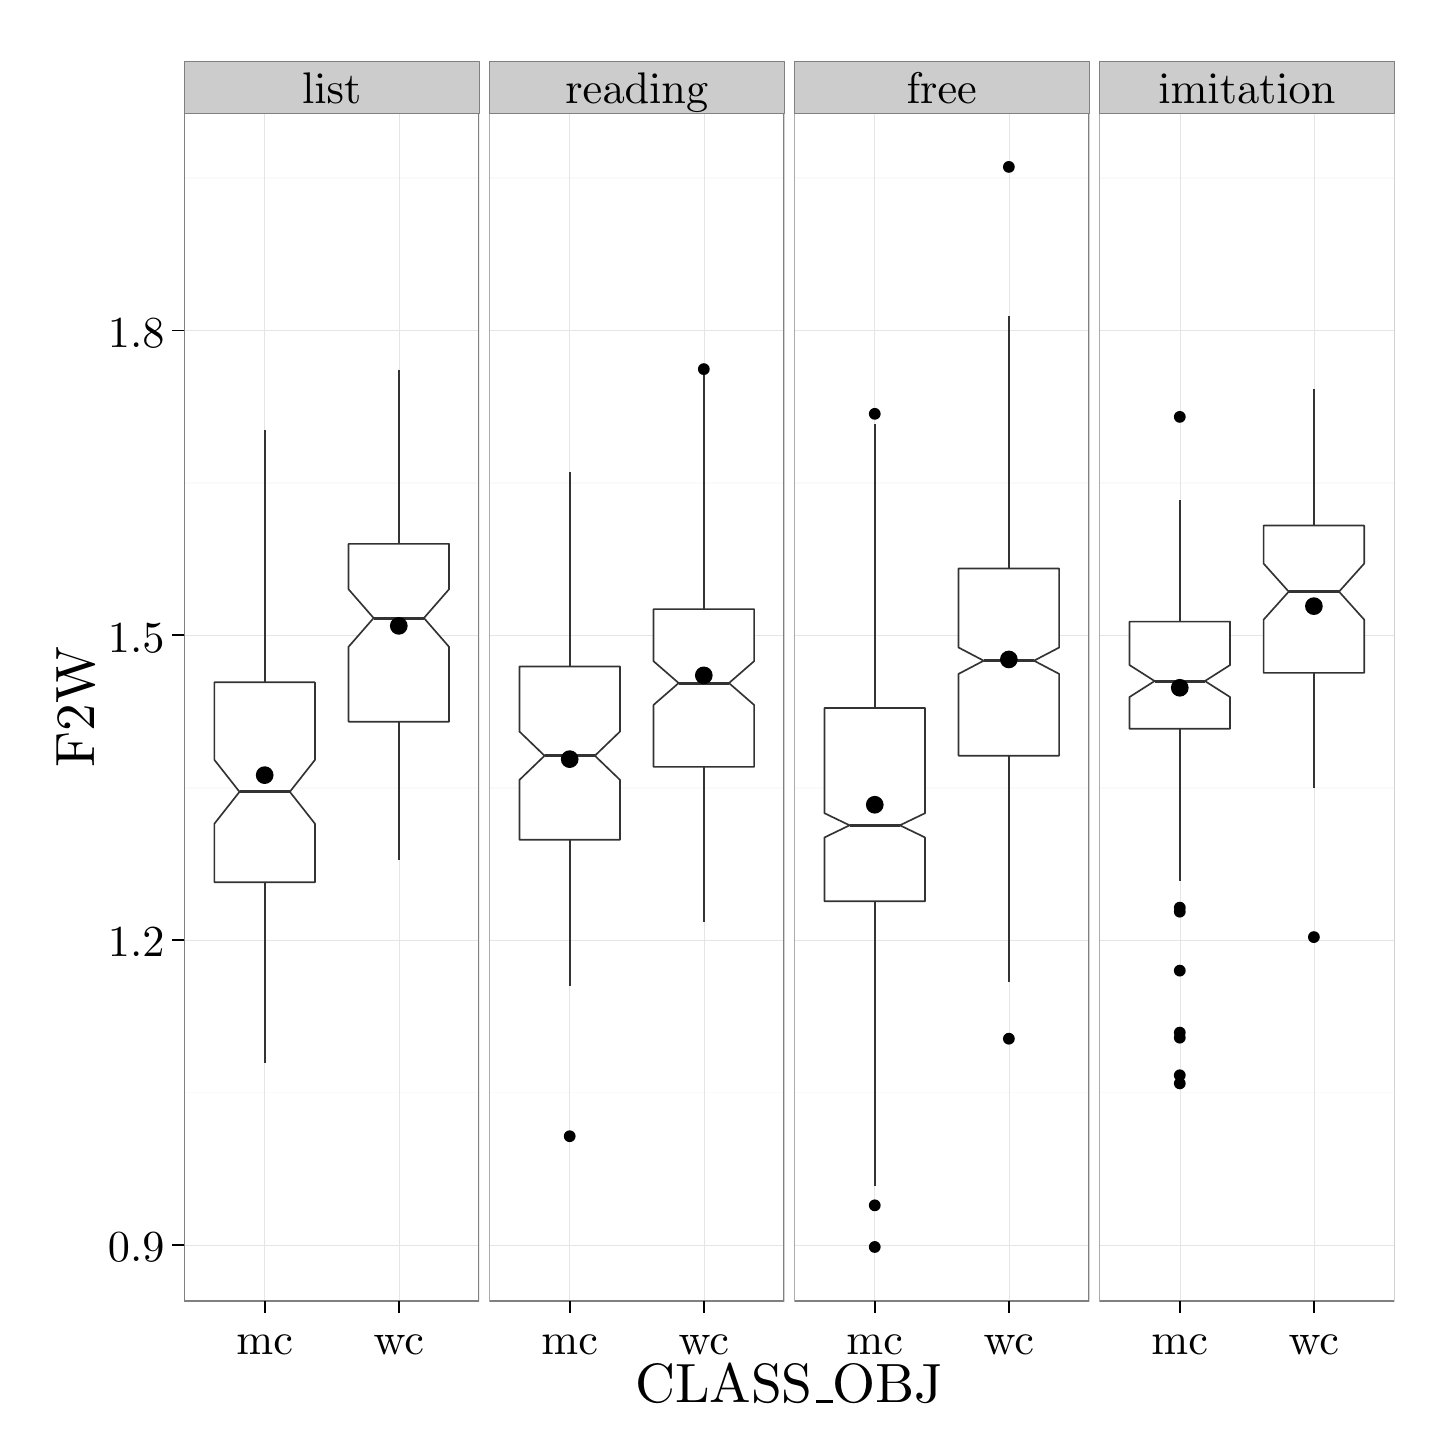
\begin{tikzpicture}[x=1pt,y=1pt]
\definecolor{fillColor}{RGB}{255,255,255}
\path[use as bounding box,fill=fillColor,fill opacity=0.00] (0,0) rectangle (505.89,505.89);
\begin{scope}
\path[clip] (  0.00,  0.00) rectangle (505.89,505.89);
\definecolor{drawColor}{RGB}{255,255,255}
\definecolor{fillColor}{RGB}{255,255,255}

\path[draw=drawColor,line width= 0.6pt,line join=round,line cap=round,fill=fillColor] (  0.00, -0.00) rectangle (505.89,505.89);
\end{scope}
\begin{scope}
\path[clip] ( 56.56, 45.77) rectangle (163.17,475.09);
\definecolor{fillColor}{RGB}{255,255,255}

\path[fill=fillColor] ( 56.56, 45.77) rectangle (163.17,475.09);
\definecolor{drawColor}{gray}{0.98}

\path[draw=drawColor,line width= 0.6pt,line join=round] ( 56.56,121.09) --
	(163.17,121.09);

\path[draw=drawColor,line width= 0.6pt,line join=round] ( 56.56,231.24) --
	(163.17,231.24);

\path[draw=drawColor,line width= 0.6pt,line join=round] ( 56.56,341.39) --
	(163.17,341.39);

\path[draw=drawColor,line width= 0.6pt,line join=round] ( 56.56,451.53) --
	(163.17,451.53);
\definecolor{drawColor}{gray}{0.90}

\path[draw=drawColor,line width= 0.2pt,line join=round] ( 56.56, 66.02) --
	(163.17, 66.02);

\path[draw=drawColor,line width= 0.2pt,line join=round] ( 56.56,176.17) --
	(163.17,176.17);

\path[draw=drawColor,line width= 0.2pt,line join=round] ( 56.56,286.31) --
	(163.17,286.31);

\path[draw=drawColor,line width= 0.2pt,line join=round] ( 56.56,396.46) --
	(163.17,396.46);

\path[draw=drawColor,line width= 0.2pt,line join=round] ( 85.64, 45.77) --
	( 85.64,475.09);

\path[draw=drawColor,line width= 0.2pt,line join=round] (134.10, 45.77) --
	(134.10,475.09);
\definecolor{drawColor}{gray}{0.20}

\path[draw=drawColor,line width= 0.6pt,line join=round] ( 85.64,269.33) -- ( 85.64,360.48);

\path[draw=drawColor,line width= 0.6pt,line join=round] ( 85.64,197.10) -- ( 85.64,131.74);

\path[draw=drawColor,line width= 0.6pt,line join=round,line cap=round,fill=fillColor] ( 67.47,269.33) --
	( 67.47,241.30) --
	( 76.55,229.77) --
	( 67.47,218.24) --
	( 67.47,197.10) --
	(103.81,197.10) --
	(103.81,218.24) --
	( 94.73,229.77) --
	(103.81,241.30) --
	(103.81,269.33) --
	( 67.47,269.33) --
	cycle;

\path[draw=drawColor,line width= 1.1pt,line join=round] ( 76.55,229.77) -- ( 94.73,229.77);

\path[draw=drawColor,line width= 0.6pt,line join=round] (134.10,319.36) -- (134.10,382.14);

\path[draw=drawColor,line width= 0.6pt,line join=round] (134.10,255.11) -- (134.10,205.17);

\path[draw=drawColor,line width= 0.6pt,line join=round,line cap=round,fill=fillColor] (115.93,319.36) --
	(115.93,302.97) --
	(125.01,292.56) --
	(115.93,282.14) --
	(115.93,255.11) --
	(152.27,255.11) --
	(152.27,282.14) --
	(143.19,292.56) --
	(152.27,302.97) --
	(152.27,319.36) --
	(115.93,319.36) --
	cycle;

\path[draw=drawColor,line width= 1.1pt,line join=round] (125.01,292.56) -- (143.19,292.56);
\definecolor{fillColor}{RGB}{0,0,0}

\path[fill=fillColor] ( 85.64,235.79) circle (  3.20);

\path[fill=fillColor] (134.10,289.73) circle (  3.20);
\definecolor{drawColor}{gray}{0.50}

\path[draw=drawColor,line width= 0.6pt,line join=round,line cap=round] ( 56.56, 45.77) rectangle (163.17,475.09);
\end{scope}
\begin{scope}
\path[clip] (166.79, 45.77) rectangle (273.40,475.09);
\definecolor{fillColor}{RGB}{255,255,255}

\path[fill=fillColor] (166.79, 45.77) rectangle (273.40,475.09);
\definecolor{drawColor}{gray}{0.98}

\path[draw=drawColor,line width= 0.6pt,line join=round] (166.79,121.09) --
	(273.40,121.09);

\path[draw=drawColor,line width= 0.6pt,line join=round] (166.79,231.24) --
	(273.40,231.24);

\path[draw=drawColor,line width= 0.6pt,line join=round] (166.79,341.39) --
	(273.40,341.39);

\path[draw=drawColor,line width= 0.6pt,line join=round] (166.79,451.53) --
	(273.40,451.53);
\definecolor{drawColor}{gray}{0.90}

\path[draw=drawColor,line width= 0.2pt,line join=round] (166.79, 66.02) --
	(273.40, 66.02);

\path[draw=drawColor,line width= 0.2pt,line join=round] (166.79,176.17) --
	(273.40,176.17);

\path[draw=drawColor,line width= 0.2pt,line join=round] (166.79,286.31) --
	(273.40,286.31);

\path[draw=drawColor,line width= 0.2pt,line join=round] (166.79,396.46) --
	(273.40,396.46);

\path[draw=drawColor,line width= 0.2pt,line join=round] (195.86, 45.77) --
	(195.86,475.09);

\path[draw=drawColor,line width= 0.2pt,line join=round] (244.32, 45.77) --
	(244.32,475.09);
\definecolor{fillColor}{RGB}{0,0,0}

\path[fill=fillColor] (195.86,105.31) circle (  2.13);
\definecolor{drawColor}{gray}{0.20}

\path[draw=drawColor,line width= 0.6pt,line join=round] (195.86,275.02) -- (195.86,345.43);

\path[draw=drawColor,line width= 0.6pt,line join=round] (195.86,212.42) -- (195.86,159.65);
\definecolor{fillColor}{RGB}{255,255,255}

\path[draw=drawColor,line width= 0.6pt,line join=round,line cap=round,fill=fillColor] (177.69,275.02) --
	(177.69,251.55) --
	(186.78,242.81) --
	(177.69,234.06) --
	(177.69,212.42) --
	(214.04,212.42) --
	(214.04,234.06) --
	(204.95,242.81) --
	(214.04,251.55) --
	(214.04,275.02) --
	(177.69,275.02) --
	cycle;

\path[draw=drawColor,line width= 1.1pt,line join=round] (186.78,242.81) -- (204.95,242.81);
\definecolor{fillColor}{RGB}{0,0,0}

\path[fill=fillColor] (244.32,382.51) circle (  2.13);

\path[draw=drawColor,line width= 0.6pt,line join=round] (244.32,295.77) -- (244.32,380.31);

\path[draw=drawColor,line width= 0.6pt,line join=round] (244.32,238.77) -- (244.32,182.78);
\definecolor{fillColor}{RGB}{255,255,255}

\path[draw=drawColor,line width= 0.6pt,line join=round,line cap=round,fill=fillColor] (226.15,295.77) --
	(226.15,276.96) --
	(235.24,269.06) --
	(226.15,261.16) --
	(226.15,238.77) --
	(262.49,238.77) --
	(262.49,261.16) --
	(253.41,269.06) --
	(262.49,276.96) --
	(262.49,295.77) --
	(226.15,295.77) --
	cycle;

\path[draw=drawColor,line width= 1.1pt,line join=round] (235.24,269.06) -- (253.41,269.06);
\definecolor{fillColor}{RGB}{0,0,0}

\path[fill=fillColor] (195.86,241.57) circle (  3.20);

\path[fill=fillColor] (244.32,271.84) circle (  3.20);
\definecolor{drawColor}{gray}{0.50}

\path[draw=drawColor,line width= 0.6pt,line join=round,line cap=round] (166.79, 45.77) rectangle (273.40,475.09);
\end{scope}
\begin{scope}
\path[clip] (277.01, 45.77) rectangle (383.62,475.09);
\definecolor{fillColor}{RGB}{255,255,255}

\path[fill=fillColor] (277.01, 45.77) rectangle (383.62,475.09);
\definecolor{drawColor}{gray}{0.98}

\path[draw=drawColor,line width= 0.6pt,line join=round] (277.01,121.09) --
	(383.62,121.09);

\path[draw=drawColor,line width= 0.6pt,line join=round] (277.01,231.24) --
	(383.62,231.24);

\path[draw=drawColor,line width= 0.6pt,line join=round] (277.01,341.39) --
	(383.62,341.39);

\path[draw=drawColor,line width= 0.6pt,line join=round] (277.01,451.53) --
	(383.62,451.53);
\definecolor{drawColor}{gray}{0.90}

\path[draw=drawColor,line width= 0.2pt,line join=round] (277.01, 66.02) --
	(383.62, 66.02);

\path[draw=drawColor,line width= 0.2pt,line join=round] (277.01,176.17) --
	(383.62,176.17);

\path[draw=drawColor,line width= 0.2pt,line join=round] (277.01,286.31) --
	(383.62,286.31);

\path[draw=drawColor,line width= 0.2pt,line join=round] (277.01,396.46) --
	(383.62,396.46);

\path[draw=drawColor,line width= 0.2pt,line join=round] (306.09, 45.77) --
	(306.09,475.09);

\path[draw=drawColor,line width= 0.2pt,line join=round] (354.55, 45.77) --
	(354.55,475.09);
\definecolor{fillColor}{RGB}{0,0,0}

\path[fill=fillColor] (306.09, 65.29) circle (  2.13);

\path[fill=fillColor] (306.09, 80.34) circle (  2.13);

\path[fill=fillColor] (306.09,366.35) circle (  2.13);
\definecolor{drawColor}{gray}{0.20}

\path[draw=drawColor,line width= 0.6pt,line join=round] (306.09,260.06) -- (306.09,362.68);

\path[draw=drawColor,line width= 0.6pt,line join=round] (306.09,190.21) -- (306.09, 87.32);
\definecolor{fillColor}{RGB}{255,255,255}

\path[draw=drawColor,line width= 0.6pt,line join=round,line cap=round,fill=fillColor] (287.91,260.06) --
	(287.91,222.04) --
	(297.00,217.66) --
	(287.91,213.27) --
	(287.91,190.21) --
	(324.26,190.21) --
	(324.26,213.27) --
	(315.17,217.66) --
	(324.26,222.04) --
	(324.26,260.06) --
	(287.91,260.06) --
	cycle;

\path[draw=drawColor,line width= 1.1pt,line join=round] (297.00,217.66) -- (315.17,217.66);
\definecolor{fillColor}{RGB}{0,0,0}

\path[fill=fillColor] (354.55,455.57) circle (  2.13);

\path[fill=fillColor] (354.55,140.55) circle (  2.13);

\path[draw=drawColor,line width= 0.6pt,line join=round] (354.55,310.45) -- (354.55,401.60);

\path[draw=drawColor,line width= 0.6pt,line join=round] (354.55,242.81) -- (354.55,161.11);
\definecolor{fillColor}{RGB}{255,255,255}

\path[draw=drawColor,line width= 0.6pt,line join=round,line cap=round,fill=fillColor] (336.37,310.45) --
	(336.37,281.90) --
	(345.46,277.14) --
	(336.37,272.37) --
	(336.37,242.81) --
	(372.72,242.81) --
	(372.72,272.37) --
	(363.63,277.14) --
	(372.72,281.90) --
	(372.72,310.45) --
	(336.37,310.45) --
	cycle;

\path[draw=drawColor,line width= 1.1pt,line join=round] (345.46,277.14) -- (363.63,277.14);
\definecolor{fillColor}{RGB}{0,0,0}

\path[fill=fillColor] (306.09,225.09) circle (  3.20);

\path[fill=fillColor] (354.55,277.59) circle (  3.20);
\definecolor{drawColor}{gray}{0.50}

\path[draw=drawColor,line width= 0.6pt,line join=round,line cap=round] (277.01, 45.77) rectangle (383.62,475.09);
\end{scope}
\begin{scope}
\path[clip] (387.24, 45.77) rectangle (493.85,475.09);
\definecolor{fillColor}{RGB}{255,255,255}

\path[fill=fillColor] (387.24, 45.77) rectangle (493.85,475.09);
\definecolor{drawColor}{gray}{0.98}

\path[draw=drawColor,line width= 0.6pt,line join=round] (387.24,121.09) --
	(493.85,121.09);

\path[draw=drawColor,line width= 0.6pt,line join=round] (387.24,231.24) --
	(493.85,231.24);

\path[draw=drawColor,line width= 0.6pt,line join=round] (387.24,341.39) --
	(493.85,341.39);

\path[draw=drawColor,line width= 0.6pt,line join=round] (387.24,451.53) --
	(493.85,451.53);
\definecolor{drawColor}{gray}{0.90}

\path[draw=drawColor,line width= 0.2pt,line join=round] (387.24, 66.02) --
	(493.85, 66.02);

\path[draw=drawColor,line width= 0.2pt,line join=round] (387.24,176.17) --
	(493.85,176.17);

\path[draw=drawColor,line width= 0.2pt,line join=round] (387.24,286.31) --
	(493.85,286.31);

\path[draw=drawColor,line width= 0.2pt,line join=round] (387.24,396.46) --
	(493.85,396.46);

\path[draw=drawColor,line width= 0.2pt,line join=round] (416.31, 45.77) --
	(416.31,475.09);

\path[draw=drawColor,line width= 0.2pt,line join=round] (464.77, 45.77) --
	(464.77,475.09);
\definecolor{fillColor}{RGB}{0,0,0}

\path[fill=fillColor] (416.31,140.92) circle (  2.13);

\path[fill=fillColor] (416.31,165.15) circle (  2.13);

\path[fill=fillColor] (416.31,186.45) circle (  2.13);

\path[fill=fillColor] (416.31,142.76) circle (  2.13);

\path[fill=fillColor] (416.31,187.92) circle (  2.13);

\path[fill=fillColor] (416.31,365.25) circle (  2.13);

\path[fill=fillColor] (416.31,124.40) circle (  2.13);

\path[fill=fillColor] (416.31,127.34) circle (  2.13);
\definecolor{drawColor}{gray}{0.20}

\path[draw=drawColor,line width= 0.6pt,line join=round] (416.31,291.27) -- (416.31,335.15);

\path[draw=drawColor,line width= 0.6pt,line join=round] (416.31,252.54) -- (416.31,197.46);
\definecolor{fillColor}{RGB}{255,255,255}

\path[draw=drawColor,line width= 0.6pt,line join=round,line cap=round,fill=fillColor] (398.14,291.27) --
	(398.14,275.57) --
	(407.22,269.79) --
	(398.14,264.01) --
	(398.14,252.54) --
	(434.48,252.54) --
	(434.48,264.01) --
	(425.40,269.79) --
	(434.48,275.57) --
	(434.48,291.27) --
	(398.14,291.27) --
	cycle;

\path[draw=drawColor,line width= 1.1pt,line join=round] (407.22,269.79) -- (425.40,269.79);
\definecolor{fillColor}{RGB}{0,0,0}

\path[fill=fillColor] (464.77,177.27) circle (  2.13);

\path[draw=drawColor,line width= 0.6pt,line join=round] (464.77,325.97) -- (464.77,375.17);

\path[draw=drawColor,line width= 0.6pt,line join=round] (464.77,272.73) -- (464.77,231.24);
\definecolor{fillColor}{RGB}{255,255,255}

\path[draw=drawColor,line width= 0.6pt,line join=round,line cap=round,fill=fillColor] (446.60,325.97) --
	(446.60,312.23) --
	(455.68,302.10) --
	(446.60,291.98) --
	(446.60,272.73) --
	(482.94,272.73) --
	(482.94,291.98) --
	(473.86,302.10) --
	(482.94,312.23) --
	(482.94,325.97) --
	(446.60,325.97) --
	cycle;

\path[draw=drawColor,line width= 1.1pt,line join=round] (455.68,302.10) -- (473.86,302.10);
\definecolor{fillColor}{RGB}{0,0,0}

\path[fill=fillColor] (416.31,267.36) circle (  3.20);

\path[fill=fillColor] (464.77,296.86) circle (  3.20);
\definecolor{drawColor}{gray}{0.50}

\path[draw=drawColor,line width= 0.6pt,line join=round,line cap=round] (387.24, 45.77) rectangle (493.85,475.09);
\end{scope}
\begin{scope}
\path[clip] (  0.00,  0.00) rectangle (505.89,505.89);
\definecolor{drawColor}{gray}{0.50}
\definecolor{fillColor}{gray}{0.80}

\path[draw=drawColor,line width= 0.2pt,line join=round,line cap=round,fill=fillColor] ( 56.56,475.09) rectangle (163.17,493.85);
\definecolor{drawColor}{RGB}{0,0,0}

\node[text=drawColor,anchor=base,inner sep=0pt, outer sep=0pt, scale=  1.60] at (109.87,478.43) {list};
\end{scope}
\begin{scope}
\path[clip] (  0.00,  0.00) rectangle (505.89,505.89);
\definecolor{drawColor}{gray}{0.50}
\definecolor{fillColor}{gray}{0.80}

\path[draw=drawColor,line width= 0.2pt,line join=round,line cap=round,fill=fillColor] (166.79,475.09) rectangle (273.40,493.85);
\definecolor{drawColor}{RGB}{0,0,0}

\node[text=drawColor,anchor=base,inner sep=0pt, outer sep=0pt, scale=  1.60] at (220.09,478.43) {reading};
\end{scope}
\begin{scope}
\path[clip] (  0.00,  0.00) rectangle (505.89,505.89);
\definecolor{drawColor}{gray}{0.50}
\definecolor{fillColor}{gray}{0.80}

\path[draw=drawColor,line width= 0.2pt,line join=round,line cap=round,fill=fillColor] (277.01,475.09) rectangle (383.62,493.85);
\definecolor{drawColor}{RGB}{0,0,0}

\node[text=drawColor,anchor=base,inner sep=0pt, outer sep=0pt, scale=  1.60] at (330.32,478.43) {free};
\end{scope}
\begin{scope}
\path[clip] (  0.00,  0.00) rectangle (505.89,505.89);
\definecolor{drawColor}{gray}{0.50}
\definecolor{fillColor}{gray}{0.80}

\path[draw=drawColor,line width= 0.2pt,line join=round,line cap=round,fill=fillColor] (387.24,475.09) rectangle (493.85,493.85);
\definecolor{drawColor}{RGB}{0,0,0}

\node[text=drawColor,anchor=base,inner sep=0pt, outer sep=0pt, scale=  1.60] at (440.54,478.43) {imitation};
\end{scope}
\begin{scope}
\path[clip] (  0.00,  0.00) rectangle (505.89,505.89);
\definecolor{drawColor}{RGB}{0,0,0}

\node[text=drawColor,anchor=base east,inner sep=0pt, outer sep=0pt, scale=  1.60] at ( 49.45, 59.99) {0.9};

\node[text=drawColor,anchor=base east,inner sep=0pt, outer sep=0pt, scale=  1.60] at ( 49.45,170.13) {1.2};

\node[text=drawColor,anchor=base east,inner sep=0pt, outer sep=0pt, scale=  1.60] at ( 49.45,280.28) {1.5};

\node[text=drawColor,anchor=base east,inner sep=0pt, outer sep=0pt, scale=  1.60] at ( 49.45,390.43) {1.8};
\end{scope}
\begin{scope}
\path[clip] (  0.00,  0.00) rectangle (505.89,505.89);
\definecolor{drawColor}{RGB}{0,0,0}

\path[draw=drawColor,line width= 0.6pt,line join=round] ( 52.30, 66.02) --
	( 56.56, 66.02);

\path[draw=drawColor,line width= 0.6pt,line join=round] ( 52.30,176.17) --
	( 56.56,176.17);

\path[draw=drawColor,line width= 0.6pt,line join=round] ( 52.30,286.31) --
	( 56.56,286.31);

\path[draw=drawColor,line width= 0.6pt,line join=round] ( 52.30,396.46) --
	( 56.56,396.46);
\end{scope}
\begin{scope}
\path[clip] (  0.00,  0.00) rectangle (505.89,505.89);
\definecolor{drawColor}{RGB}{0,0,0}

\path[draw=drawColor,line width= 0.6pt,line join=round] ( 85.64, 41.50) --
	( 85.64, 45.77);

\path[draw=drawColor,line width= 0.6pt,line join=round] (134.10, 41.50) --
	(134.10, 45.77);
\end{scope}
\begin{scope}
\path[clip] (  0.00,  0.00) rectangle (505.89,505.89);
\definecolor{drawColor}{RGB}{0,0,0}

\node[text=drawColor,anchor=base,inner sep=0pt, outer sep=0pt, scale=  1.60] at ( 85.64, 26.59) {mc};

\node[text=drawColor,anchor=base,inner sep=0pt, outer sep=0pt, scale=  1.60] at (134.10, 26.59) {wc};
\end{scope}
\begin{scope}
\path[clip] (  0.00,  0.00) rectangle (505.89,505.89);
\definecolor{drawColor}{RGB}{0,0,0}

\path[draw=drawColor,line width= 0.6pt,line join=round] (195.86, 41.50) --
	(195.86, 45.77);

\path[draw=drawColor,line width= 0.6pt,line join=round] (244.32, 41.50) --
	(244.32, 45.77);
\end{scope}
\begin{scope}
\path[clip] (  0.00,  0.00) rectangle (505.89,505.89);
\definecolor{drawColor}{RGB}{0,0,0}

\node[text=drawColor,anchor=base,inner sep=0pt, outer sep=0pt, scale=  1.60] at (195.86, 26.59) {mc};

\node[text=drawColor,anchor=base,inner sep=0pt, outer sep=0pt, scale=  1.60] at (244.32, 26.59) {wc};
\end{scope}
\begin{scope}
\path[clip] (  0.00,  0.00) rectangle (505.89,505.89);
\definecolor{drawColor}{RGB}{0,0,0}

\path[draw=drawColor,line width= 0.6pt,line join=round] (306.09, 41.50) --
	(306.09, 45.77);

\path[draw=drawColor,line width= 0.6pt,line join=round] (354.55, 41.50) --
	(354.55, 45.77);
\end{scope}
\begin{scope}
\path[clip] (  0.00,  0.00) rectangle (505.89,505.89);
\definecolor{drawColor}{RGB}{0,0,0}

\node[text=drawColor,anchor=base,inner sep=0pt, outer sep=0pt, scale=  1.60] at (306.09, 26.59) {mc};

\node[text=drawColor,anchor=base,inner sep=0pt, outer sep=0pt, scale=  1.60] at (354.55, 26.59) {wc};
\end{scope}
\begin{scope}
\path[clip] (  0.00,  0.00) rectangle (505.89,505.89);
\definecolor{drawColor}{RGB}{0,0,0}

\path[draw=drawColor,line width= 0.6pt,line join=round] (416.31, 41.50) --
	(416.31, 45.77);

\path[draw=drawColor,line width= 0.6pt,line join=round] (464.77, 41.50) --
	(464.77, 45.77);
\end{scope}
\begin{scope}
\path[clip] (  0.00,  0.00) rectangle (505.89,505.89);
\definecolor{drawColor}{RGB}{0,0,0}

\node[text=drawColor,anchor=base,inner sep=0pt, outer sep=0pt, scale=  1.60] at (416.31, 26.59) {mc};

\node[text=drawColor,anchor=base,inner sep=0pt, outer sep=0pt, scale=  1.60] at (464.77, 26.59) {wc};
\end{scope}
\begin{scope}
\path[clip] (  0.00,  0.00) rectangle (505.89,505.89);
\definecolor{drawColor}{RGB}{0,0,0}

\node[text=drawColor,anchor=base,inner sep=0pt, outer sep=0pt, scale=  2.00] at (275.20,  9.03) {CLASS{\_{}}OBJ};
\end{scope}
\begin{scope}
\path[clip] (  0.00,  0.00) rectangle (505.89,505.89);
\definecolor{drawColor}{RGB}{0,0,0}

\node[text=drawColor,rotate= 90.00,anchor=base,inner sep=0pt, outer sep=0pt, scale=  2.00] at ( 24.12,260.43) {F2W};
\end{scope}
\end{tikzpicture}
} 
	\caption{\textsc{nurse} (F2) by style and social class}
	\label{fig.box.f2w.nurse.styleclass}
\end{figure}

The interaction of style and social class is again one where we are looking at differences in degree more than in nature.
If one examines the boxplots in Figure \ref{fig.box.f2w.nurse.styleclass}, which are sorted from most formal register (word list) on the left to least formal one (accent perform\is{accent performance}ance) on the right, it is clear that the pattern is pretty much the same in all of them.
Boxes that visualise the data collected from middle-class interviewees (always the left one in each panel) are consistently lower than the corresponding ones for working-class speakers, which illustrates once again that working-class speakers have more Scouse \textsc{nurse} variants than middle-class Liverpudlians (cf. Figure \ref{fig.scatter.f2w.nurse.genderclass}).
T-tests confirm for the means what the notches in the box plots do for the medians: the class difference is statistically significant for the word list (t(188.089) = -8.096, p < 0.001), the reading passage (t(255.085) = -5.524, p < 0.001), spontaneous speech (t(1087.269) = -17.359, p < 0.001), and accent imitation\is{accent performance} (t(153.537) = -4.744, p < 0.001).

\begin{table}[h!]
	\centering
	\caption{\textsc{nurse} (F2): t-tests of style by social class}
	\label{tab.nurse.classstyle.pvalues}
	\begin{tabular}{lrrrrrr}
		\hline
		test & \multicolumn{3}{c}{middle class} & \multicolumn{3}{c}{working class}\\
		& t & df & p & t & df & p\\
		\hline
		list-reading & \ensuremath{-0.923} & 189.641 & 0.357 & 3.019 & 210.158 & 0.003\\
		list-free & 1.971 & 130.746 & 0.051 & 2.473 & 147.930 & 0.015\\
		list-imitation\is{accent performance} & \ensuremath{-4.894} & 192.492 & < 0.001 & \ensuremath{-1.107} & 153.071 & 0.270\\
		reading-free & 3.870 & 209.460 & < 0.001 & \ensuremath{-1.254} & 216.848 & 0.211\\
		reading-imitation\is{accent performance} & \ensuremath{-4.684} & 233.144 & < 0.001 & \ensuremath{-4.039} & 157.841 & < 0.001\\
		free-imitation\is{accent performance} & \ensuremath{-9.346} & 172.419 & < 0.001 & \ensuremath{-3.684} & 101.284 & < 0.001\\
		\hline			
	\end{tabular}
\end{table}

Figure \ref{fig.box.f2w.nurse.styleclass} also shows that while the class effect is generally the same for all styles, it is more pronounced in the reading list and free speech registers, than when people read out a text or put on a particularly strong Scouse accent.
Both classes have the most Scouse realisations in the accent perform\is{accent performance}ance, but apart from that the order of styles is different (cf. Table \ref{tab.nurse.classstyle.pvalues} for tests of significance).
For middle-class speakers `imitation\is{accent performance}' is significantly more Scouse than `reading', which is in second place and followed by the word list (which does not differ significantly from `reading').
The most central (least Scouse) variants are found in spontaneous speech, which is very close to forming a statistically robust contrast with the word list.
When we look at working-class subjects, the order from most Scouse to least Scouse is: `imitation\is{accent performance}', `list', `free', and `reading'.
The first and the last two of these four are not significantly different from each other, so that statistically speaking we have a more Scouse block `imitation\is{accent performance}/list', and a less Scouse pair `free/reading'.
None of these orders corresponds to what would have been expected based on the traditional formality scale.

\subsubsection{Age and social class}
\label{sec.prod.res.vow.nurse.f2.styleage}

\begin{figure}[h!]
	\centering
		\definecolor{shadecolor}{rgb}{0.969, 0.969, 0.969}
		\resizebox{0.5\linewidth}{!}{% Created by tikzDevice version 0.8.1 on 2016-02-09 02:15:03
% !TEX encoding = UTF-8 Unicode
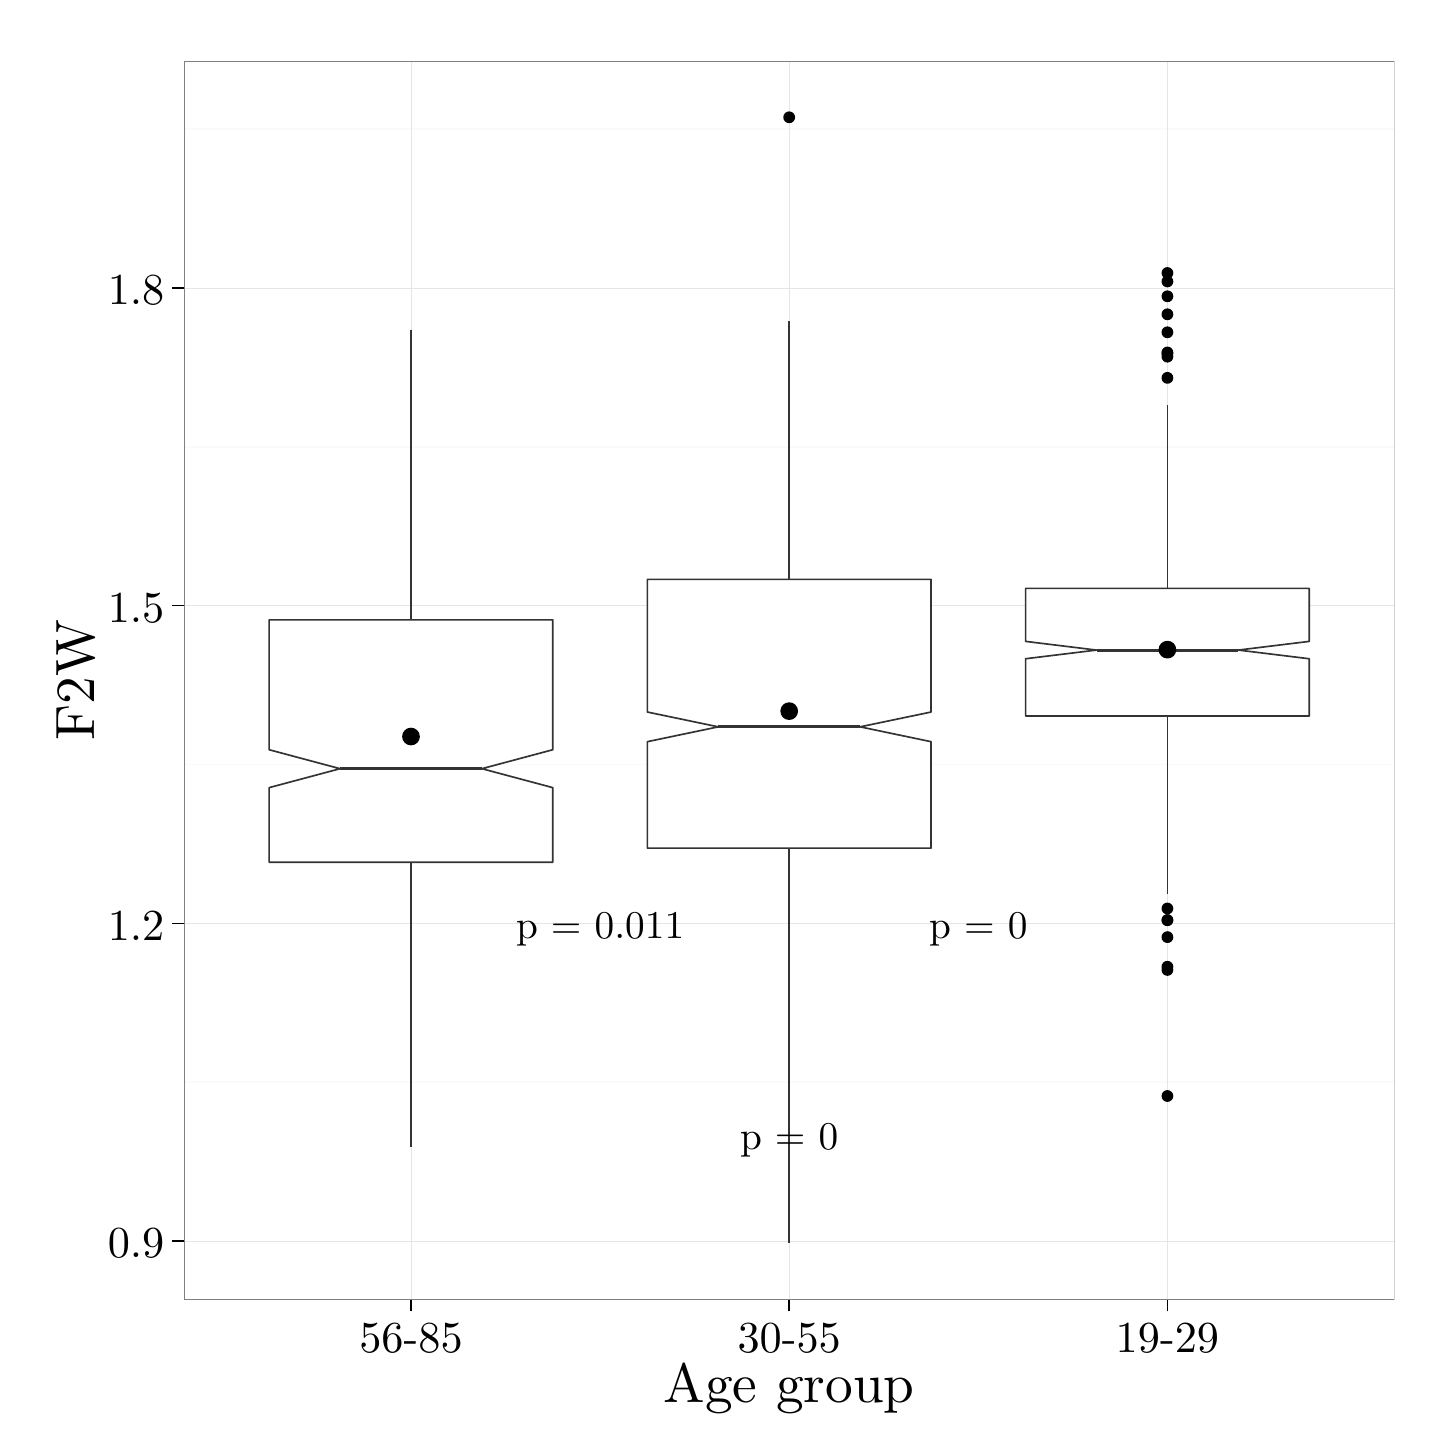
\begin{tikzpicture}[x=1pt,y=1pt]
\definecolor{fillColor}{RGB}{255,255,255}
\path[use as bounding box,fill=fillColor,fill opacity=0.00] (0,0) rectangle (505.89,505.89);
\begin{scope}
\path[clip] (  0.00,  0.00) rectangle (505.89,505.89);
\definecolor{drawColor}{RGB}{255,255,255}
\definecolor{fillColor}{RGB}{255,255,255}

\path[draw=drawColor,line width= 0.6pt,line join=round,line cap=round,fill=fillColor] (  0.00, -0.00) rectangle (505.89,505.89);
\end{scope}
\begin{scope}
\path[clip] ( 56.50, 46.31) rectangle (493.85,493.84);
\definecolor{fillColor}{RGB}{255,255,255}

\path[fill=fillColor] ( 56.50, 46.31) rectangle (493.85,493.84);
\definecolor{drawColor}{gray}{0.98}

\path[draw=drawColor,line width= 0.6pt,line join=round] ( 56.50,124.83) --
	(493.85,124.83);

\path[draw=drawColor,line width= 0.6pt,line join=round] ( 56.50,239.65) --
	(493.85,239.65);

\path[draw=drawColor,line width= 0.6pt,line join=round] ( 56.50,354.47) --
	(493.85,354.47);

\path[draw=drawColor,line width= 0.6pt,line join=round] ( 56.50,469.29) --
	(493.85,469.29);
\definecolor{drawColor}{gray}{0.90}

\path[draw=drawColor,line width= 0.2pt,line join=round] ( 56.50, 67.42) --
	(493.85, 67.42);

\path[draw=drawColor,line width= 0.2pt,line join=round] ( 56.50,182.24) --
	(493.85,182.24);

\path[draw=drawColor,line width= 0.2pt,line join=round] ( 56.50,297.06) --
	(493.85,297.06);

\path[draw=drawColor,line width= 0.2pt,line join=round] ( 56.50,411.88) --
	(493.85,411.88);

\path[draw=drawColor,line width= 0.2pt,line join=round] (138.51, 46.31) --
	(138.51,493.84);

\path[draw=drawColor,line width= 0.2pt,line join=round] (275.17, 46.31) --
	(275.17,493.84);

\path[draw=drawColor,line width= 0.2pt,line join=round] (411.84, 46.31) --
	(411.84,493.84);
\definecolor{drawColor}{gray}{0.20}

\path[draw=drawColor,line width= 0.6pt,line join=round] (138.51,291.89) -- (138.51,396.57);

\path[draw=drawColor,line width= 0.6pt,line join=round] (138.51,204.34) -- (138.51,101.48);

\path[draw=drawColor,line width= 0.6pt,line join=round,line cap=round,fill=fillColor] ( 87.25,291.89) --
	( 87.25,244.97) --
	(112.88,238.12) --
	( 87.25,231.27) --
	( 87.25,204.34) --
	(189.76,204.34) --
	(189.76,231.27) --
	(164.13,238.12) --
	(189.76,244.97) --
	(189.76,291.89) --
	( 87.25,291.89) --
	cycle;

\path[draw=drawColor,line width= 1.1pt,line join=round] (112.88,238.12) -- (164.13,238.12);
\definecolor{fillColor}{RGB}{0,0,0}

\path[fill=fillColor] (275.17,473.50) circle (  2.13);

\path[draw=drawColor,line width= 0.6pt,line join=round] (275.17,306.53) -- (275.17,400.02);

\path[draw=drawColor,line width= 0.6pt,line join=round] (275.17,209.41) -- (275.17, 66.65);
\definecolor{fillColor}{RGB}{255,255,255}

\path[draw=drawColor,line width= 0.6pt,line join=round,line cap=round,fill=fillColor] (223.92,306.53) --
	(223.92,258.59) --
	(249.55,253.24) --
	(223.92,247.88) --
	(223.92,209.41) --
	(326.43,209.41) --
	(326.43,247.88) --
	(300.80,253.24) --
	(326.43,258.59) --
	(326.43,306.53) --
	(223.92,306.53) --
	cycle;

\path[draw=drawColor,line width= 1.1pt,line join=round] (249.55,253.24) -- (300.80,253.24);
\definecolor{fillColor}{RGB}{0,0,0}

\path[fill=fillColor] (411.84,187.60) circle (  2.13);

\path[fill=fillColor] (411.84,183.39) circle (  2.13);

\path[fill=fillColor] (411.84,165.40) circle (  2.13);

\path[fill=fillColor] (411.84,177.26) circle (  2.13);

\path[fill=fillColor] (411.84,183.39) circle (  2.13);

\path[fill=fillColor] (411.84,166.55) circle (  2.13);

\path[fill=fillColor] (411.84,119.85) circle (  2.13);

\path[fill=fillColor] (411.84,379.35) circle (  2.13);

\path[fill=fillColor] (411.84,417.24) circle (  2.13);

\path[fill=fillColor] (411.84,402.31) circle (  2.13);

\path[fill=fillColor] (411.84,395.81) circle (  2.13);

\path[fill=fillColor] (411.84,408.82) circle (  2.13);

\path[fill=fillColor] (411.84,388.15) circle (  2.13);

\path[fill=fillColor] (411.84,387.00) circle (  2.13);

\path[fill=fillColor] (411.84,388.53) circle (  2.13);

\path[fill=fillColor] (411.84,414.18) circle (  2.13);

\path[draw=drawColor,line width= 0.6pt,line join=round] (411.84,303.28) -- (411.84,369.40);

\path[draw=drawColor,line width= 0.6pt,line join=round] (411.84,257.16) -- (411.84,192.95);
\definecolor{fillColor}{RGB}{255,255,255}

\path[draw=drawColor,line width= 0.6pt,line join=round,line cap=round,fill=fillColor] (360.59,303.28) --
	(360.59,284.12) --
	(386.22,280.98) --
	(360.59,277.85) --
	(360.59,257.16) --
	(463.09,257.16) --
	(463.09,277.85) --
	(437.47,280.98) --
	(463.09,284.12) --
	(463.09,303.28) --
	(360.59,303.28) --
	cycle;

\path[draw=drawColor,line width= 1.1pt,line join=round] (386.22,280.98) -- (437.47,280.98);
\definecolor{fillColor}{RGB}{0,0,0}

\path[fill=fillColor] (138.51,249.74) circle (  3.20);

\path[fill=fillColor] (275.17,258.92) circle (  3.20);

\path[fill=fillColor] (411.84,281.14) circle (  3.20);
\definecolor{drawColor}{RGB}{0,0,0}

\node[text=drawColor,anchor=base,inner sep=0pt, outer sep=0pt, scale=  1.42] at (206.84,176.89) {p = 0.011};

\node[text=drawColor,anchor=base,inner sep=0pt, outer sep=0pt, scale=  1.42] at (343.51,176.89) {p = 0};

\node[text=drawColor,anchor=base,inner sep=0pt, outer sep=0pt, scale=  1.42] at (275.17,100.35) {p = 0};
\definecolor{drawColor}{gray}{0.50}

\path[draw=drawColor,line width= 0.6pt,line join=round,line cap=round] ( 56.50, 46.31) rectangle (493.85,493.84);
\end{scope}
\begin{scope}
\path[clip] (  0.00,  0.00) rectangle (505.89,505.89);
\definecolor{drawColor}{RGB}{0,0,0}

\node[text=drawColor,anchor=base east,inner sep=0pt, outer sep=0pt, scale=  1.60] at ( 49.39, 61.38) {0.9};

\node[text=drawColor,anchor=base east,inner sep=0pt, outer sep=0pt, scale=  1.60] at ( 49.39,176.20) {1.2};

\node[text=drawColor,anchor=base east,inner sep=0pt, outer sep=0pt, scale=  1.60] at ( 49.39,291.03) {1.5};

\node[text=drawColor,anchor=base east,inner sep=0pt, outer sep=0pt, scale=  1.60] at ( 49.39,405.85) {1.8};
\end{scope}
\begin{scope}
\path[clip] (  0.00,  0.00) rectangle (505.89,505.89);
\definecolor{drawColor}{RGB}{0,0,0}

\path[draw=drawColor,line width= 0.6pt,line join=round] ( 52.24, 67.42) --
	( 56.50, 67.42);

\path[draw=drawColor,line width= 0.6pt,line join=round] ( 52.24,182.24) --
	( 56.50,182.24);

\path[draw=drawColor,line width= 0.6pt,line join=round] ( 52.24,297.06) --
	( 56.50,297.06);

\path[draw=drawColor,line width= 0.6pt,line join=round] ( 52.24,411.88) --
	( 56.50,411.88);
\end{scope}
\begin{scope}
\path[clip] (  0.00,  0.00) rectangle (505.89,505.89);
\definecolor{drawColor}{RGB}{0,0,0}

\path[draw=drawColor,line width= 0.6pt,line join=round] (138.51, 42.04) --
	(138.51, 46.31);

\path[draw=drawColor,line width= 0.6pt,line join=round] (275.17, 42.04) --
	(275.17, 46.31);

\path[draw=drawColor,line width= 0.6pt,line join=round] (411.84, 42.04) --
	(411.84, 46.31);
\end{scope}
\begin{scope}
\path[clip] (  0.00,  0.00) rectangle (505.89,505.89);
\definecolor{drawColor}{RGB}{0,0,0}

\node[text=drawColor,anchor=base,inner sep=0pt, outer sep=0pt, scale=  1.60] at (138.51, 27.13) {56-85};

\node[text=drawColor,anchor=base,inner sep=0pt, outer sep=0pt, scale=  1.60] at (275.17, 27.13) {30-55};

\node[text=drawColor,anchor=base,inner sep=0pt, outer sep=0pt, scale=  1.60] at (411.84, 27.13) {19-29};
\end{scope}
\begin{scope}
\path[clip] (  0.00,  0.00) rectangle (505.89,505.89);
\definecolor{drawColor}{RGB}{0,0,0}

\node[text=drawColor,anchor=base,inner sep=0pt, outer sep=0pt, scale=  2.00] at (275.17,  9.03) {Age group};
\end{scope}
\begin{scope}
\path[clip] (  0.00,  0.00) rectangle (505.89,505.89);
\definecolor{drawColor}{RGB}{0,0,0}

\node[text=drawColor,rotate= 90.00,anchor=base,inner sep=0pt, outer sep=0pt, scale=  2.00] at ( 24.12,270.08) {F2W};
\end{scope}
\end{tikzpicture}
} 
	\caption{\textsc{nurse} (F2) by age}
	\label{fig.box.f2.nurse.tot}
\end{figure}

In addition to style, social class also interacts significantly with age group, but before we turn to this interaction we will first have a quick look at age as a main effect, where a very clear and simple picture emerges (Figure \ref{fig.box.f2.nurse.tot}).
F2 values increase significantly from the oldest to the middle-aged group (t(914.871) = 2.558, p = 0.011), and continue to rise from the middle to the youngest speakers (t(1347.58) = 7.955, p < 0.001).
Middle-aged speakers have thus a fronter \textsc{nurse} than the oldest subjects in this sample, and speakers in the youngest group have, in turn, a significantly fronter vowel than Liverpudlians of their parents' generation.
However, things are slightly more complicated, as an analysis of the age X social class interaction reveals.

\begin{figure}[h!]
	\centering
	\begin{subfigure}{.49\textwidth}
		\centering
			\definecolor{shadecolor}{rgb}{0.969, 0.969, 0.969}
			\resizebox{\linewidth}{!}{% Created by tikzDevice version 0.8.1 on 2016-02-09 02:15:06
% !TEX encoding = UTF-8 Unicode
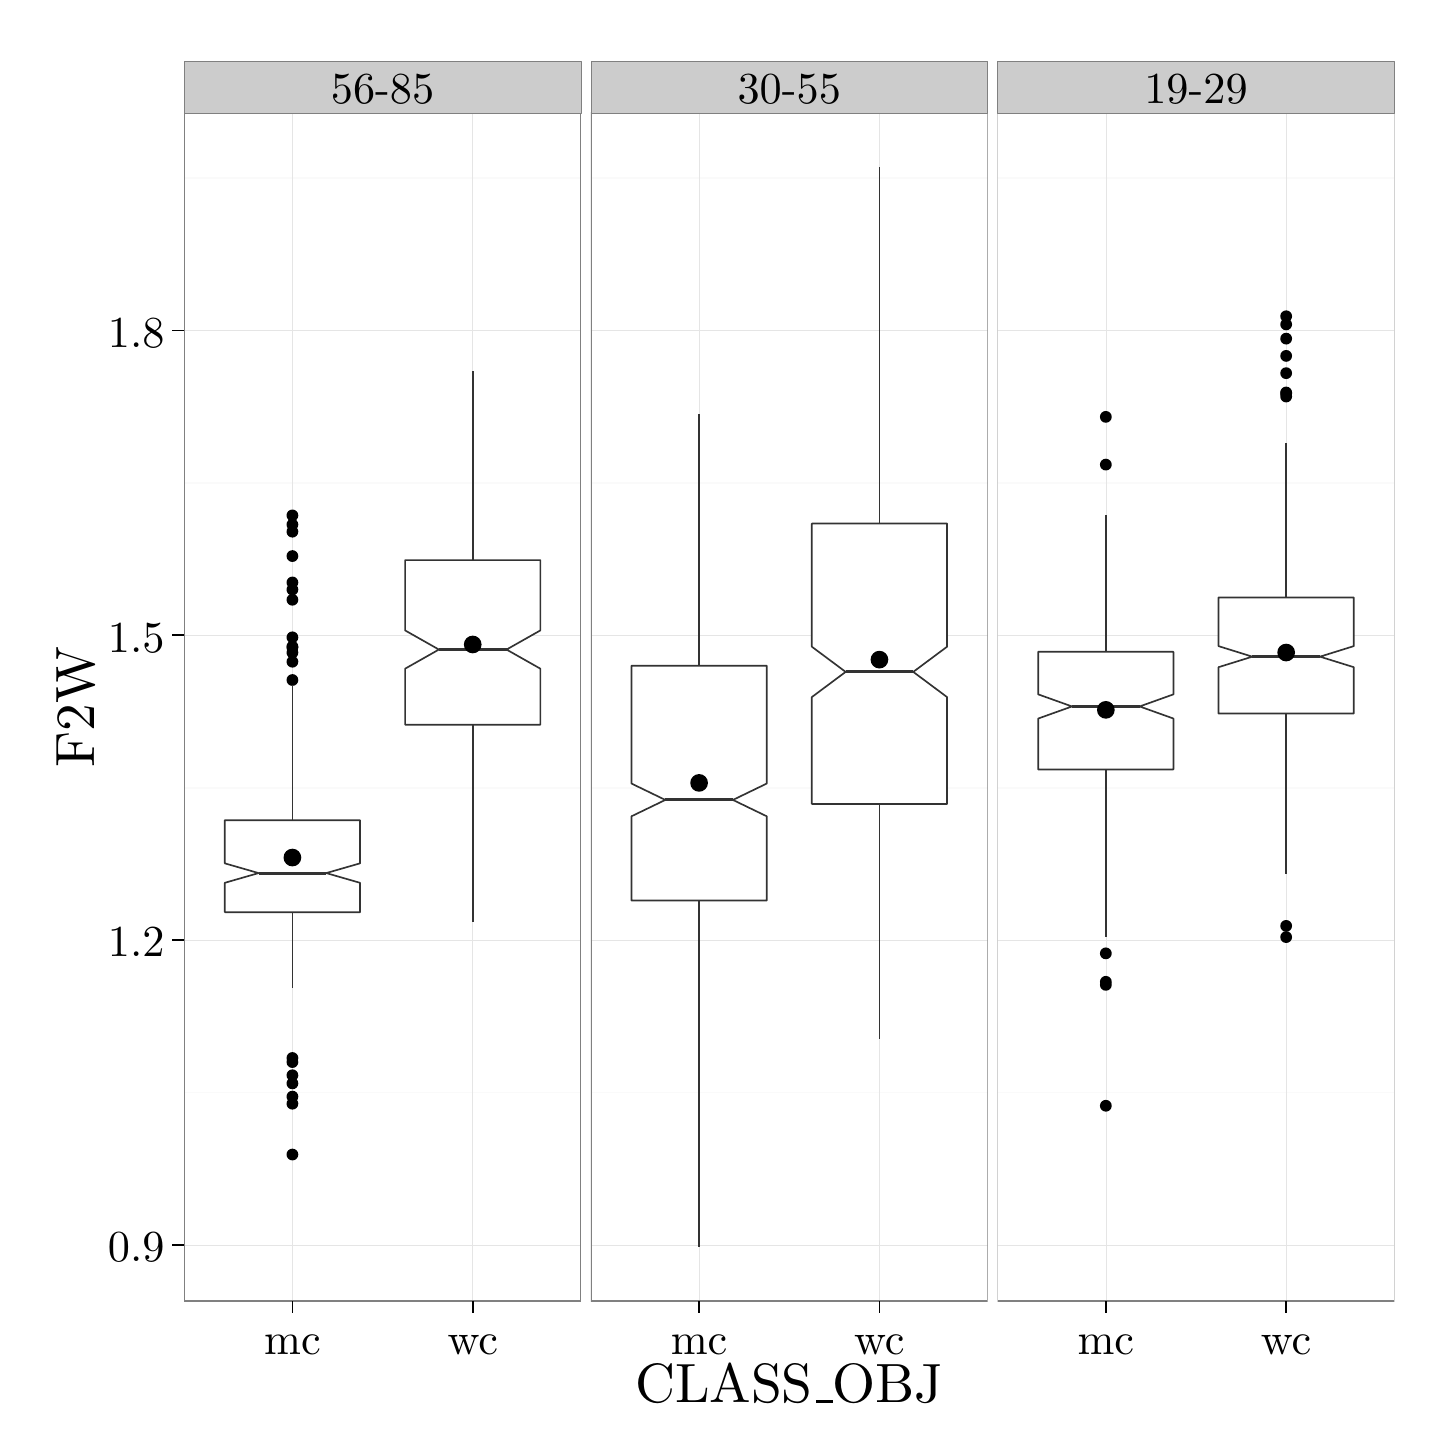
\begin{tikzpicture}[x=1pt,y=1pt]
\definecolor{fillColor}{RGB}{255,255,255}
\path[use as bounding box,fill=fillColor,fill opacity=0.00] (0,0) rectangle (505.89,505.89);
\begin{scope}
\path[clip] (  0.00,  0.00) rectangle (505.89,505.89);
\definecolor{drawColor}{RGB}{255,255,255}
\definecolor{fillColor}{RGB}{255,255,255}

\path[draw=drawColor,line width= 0.6pt,line join=round,line cap=round,fill=fillColor] (  0.00, -0.00) rectangle (505.89,505.89);
\end{scope}
\begin{scope}
\path[clip] ( 56.56, 45.77) rectangle (199.92,475.09);
\definecolor{fillColor}{RGB}{255,255,255}

\path[fill=fillColor] ( 56.56, 45.77) rectangle (199.92,475.09);
\definecolor{drawColor}{gray}{0.98}

\path[draw=drawColor,line width= 0.6pt,line join=round] ( 56.56,121.09) --
	(199.92,121.09);

\path[draw=drawColor,line width= 0.6pt,line join=round] ( 56.56,231.24) --
	(199.92,231.24);

\path[draw=drawColor,line width= 0.6pt,line join=round] ( 56.56,341.39) --
	(199.92,341.39);

\path[draw=drawColor,line width= 0.6pt,line join=round] ( 56.56,451.53) --
	(199.92,451.53);
\definecolor{drawColor}{gray}{0.90}

\path[draw=drawColor,line width= 0.2pt,line join=round] ( 56.56, 66.02) --
	(199.92, 66.02);

\path[draw=drawColor,line width= 0.2pt,line join=round] ( 56.56,176.17) --
	(199.92,176.17);

\path[draw=drawColor,line width= 0.2pt,line join=round] ( 56.56,286.31) --
	(199.92,286.31);

\path[draw=drawColor,line width= 0.2pt,line join=round] ( 56.56,396.46) --
	(199.92,396.46);

\path[draw=drawColor,line width= 0.2pt,line join=round] ( 95.66, 45.77) --
	( 95.66,475.09);

\path[draw=drawColor,line width= 0.2pt,line join=round] (160.82, 45.77) --
	(160.82,475.09);
\definecolor{fillColor}{RGB}{0,0,0}

\path[fill=fillColor] ( 95.66,119.63) circle (  2.13);

\path[fill=fillColor] ( 95.66,132.11) circle (  2.13);

\path[fill=fillColor] ( 95.66, 98.70) circle (  2.13);

\path[fill=fillColor] ( 95.66,117.06) circle (  2.13);

\path[fill=fillColor] ( 95.66,285.58) circle (  2.13);

\path[fill=fillColor] ( 95.66,282.28) circle (  2.13);

\path[fill=fillColor] ( 95.66,276.77) circle (  2.13);

\path[fill=fillColor] ( 95.66,270.16) circle (  2.13);

\path[fill=fillColor] ( 95.66,299.16) circle (  2.13);

\path[fill=fillColor] ( 95.66,326.33) circle (  2.13);

\path[fill=fillColor] ( 95.66,302.84) circle (  2.13);

\path[fill=fillColor] ( 95.66,280.07) circle (  2.13);

\path[fill=fillColor] ( 95.66,305.41) circle (  2.13);

\path[fill=fillColor] ( 95.66,281.91) circle (  2.13);

\path[fill=fillColor] ( 95.66,314.95) circle (  2.13);

\path[fill=fillColor] ( 95.66,124.40) circle (  2.13);

\path[fill=fillColor] ( 95.66,127.34) circle (  2.13);

\path[fill=fillColor] ( 95.66,323.76) circle (  2.13);

\path[fill=fillColor] ( 95.66,329.64) circle (  2.13);

\path[fill=fillColor] ( 95.66,133.58) circle (  2.13);
\definecolor{drawColor}{gray}{0.20}

\path[draw=drawColor,line width= 0.6pt,line join=round] ( 95.66,219.49) -- ( 95.66,268.32);

\path[draw=drawColor,line width= 0.6pt,line join=round] ( 95.66,186.26) -- ( 95.66,158.91);
\definecolor{fillColor}{RGB}{255,255,255}

\path[draw=drawColor,line width= 0.6pt,line join=round,line cap=round,fill=fillColor] ( 71.23,219.49) --
	( 71.23,203.92) --
	( 83.44,200.40) --
	( 71.23,196.88) --
	( 71.23,186.26) --
	(120.10,186.26) --
	(120.10,196.88) --
	(107.88,200.40) --
	(120.10,203.92) --
	(120.10,219.49) --
	( 71.23,219.49) --
	cycle;

\path[draw=drawColor,line width= 1.1pt,line join=round] ( 83.44,200.40) -- (107.88,200.40);

\path[draw=drawColor,line width= 0.6pt,line join=round] (160.82,313.48) -- (160.82,381.77);

\path[draw=drawColor,line width= 0.6pt,line join=round] (160.82,254.00) -- (160.82,182.78);

\path[draw=drawColor,line width= 0.6pt,line join=round,line cap=round,fill=fillColor] (136.39,313.48) --
	(136.39,288.08) --
	(148.60,281.17) --
	(136.39,274.26) --
	(136.39,254.00) --
	(185.25,254.00) --
	(185.25,274.26) --
	(173.04,281.17) --
	(185.25,288.08) --
	(185.25,313.48) --
	(136.39,313.48) --
	cycle;

\path[draw=drawColor,line width= 1.1pt,line join=round] (148.60,281.17) -- (173.04,281.17);
\definecolor{fillColor}{RGB}{0,0,0}

\path[fill=fillColor] ( 95.66,206.01) circle (  3.20);

\path[fill=fillColor] (160.82,283.00) circle (  3.20);
\definecolor{drawColor}{gray}{0.50}

\path[draw=drawColor,line width= 0.6pt,line join=round,line cap=round] ( 56.56, 45.77) rectangle (199.92,475.09);
\end{scope}
\begin{scope}
\path[clip] (203.53, 45.77) rectangle (346.88,475.09);
\definecolor{fillColor}{RGB}{255,255,255}

\path[fill=fillColor] (203.53, 45.77) rectangle (346.88,475.09);
\definecolor{drawColor}{gray}{0.98}

\path[draw=drawColor,line width= 0.6pt,line join=round] (203.53,121.09) --
	(346.88,121.09);

\path[draw=drawColor,line width= 0.6pt,line join=round] (203.53,231.24) --
	(346.88,231.24);

\path[draw=drawColor,line width= 0.6pt,line join=round] (203.53,341.39) --
	(346.88,341.39);

\path[draw=drawColor,line width= 0.6pt,line join=round] (203.53,451.53) --
	(346.88,451.53);
\definecolor{drawColor}{gray}{0.90}

\path[draw=drawColor,line width= 0.2pt,line join=round] (203.53, 66.02) --
	(346.88, 66.02);

\path[draw=drawColor,line width= 0.2pt,line join=round] (203.53,176.17) --
	(346.88,176.17);

\path[draw=drawColor,line width= 0.2pt,line join=round] (203.53,286.31) --
	(346.88,286.31);

\path[draw=drawColor,line width= 0.2pt,line join=round] (203.53,396.46) --
	(346.88,396.46);

\path[draw=drawColor,line width= 0.2pt,line join=round] (242.62, 45.77) --
	(242.62,475.09);

\path[draw=drawColor,line width= 0.2pt,line join=round] (307.78, 45.77) --
	(307.78,475.09);
\definecolor{drawColor}{gray}{0.20}

\path[draw=drawColor,line width= 0.6pt,line join=round] (242.62,275.30) -- (242.62,366.35);

\path[draw=drawColor,line width= 0.6pt,line join=round] (242.62,190.49) -- (242.62, 65.29);

\path[draw=drawColor,line width= 0.6pt,line join=round,line cap=round,fill=fillColor] (218.19,275.30) --
	(218.19,232.75) --
	(230.41,226.83) --
	(218.19,220.92) --
	(218.19,190.49) --
	(267.06,190.49) --
	(267.06,220.92) --
	(254.84,226.83) --
	(267.06,232.75) --
	(267.06,275.30) --
	(218.19,275.30) --
	cycle;

\path[draw=drawColor,line width= 1.1pt,line join=round] (230.41,226.83) -- (254.84,226.83);

\path[draw=drawColor,line width= 0.6pt,line join=round] (307.78,326.70) -- (307.78,455.57);

\path[draw=drawColor,line width= 0.6pt,line join=round] (307.78,225.37) -- (307.78,140.55);

\path[draw=drawColor,line width= 0.6pt,line join=round,line cap=round,fill=fillColor] (283.35,326.70) --
	(283.35,282.20) --
	(295.57,273.10) --
	(283.35,263.99) --
	(283.35,225.37) --
	(332.22,225.37) --
	(332.22,263.99) --
	(320.00,273.10) --
	(332.22,282.20) --
	(332.22,326.70) --
	(283.35,326.70) --
	cycle;

\path[draw=drawColor,line width= 1.1pt,line join=round] (295.57,273.10) -- (320.00,273.10);
\definecolor{fillColor}{RGB}{0,0,0}

\path[fill=fillColor] (242.62,232.99) circle (  3.20);

\path[fill=fillColor] (307.78,277.52) circle (  3.20);
\definecolor{drawColor}{gray}{0.50}

\path[draw=drawColor,line width= 0.6pt,line join=round,line cap=round] (203.53, 45.77) rectangle (346.88,475.09);
\end{scope}
\begin{scope}
\path[clip] (350.49, 45.77) rectangle (493.85,475.09);
\definecolor{fillColor}{RGB}{255,255,255}

\path[fill=fillColor] (350.49, 45.77) rectangle (493.85,475.09);
\definecolor{drawColor}{gray}{0.98}

\path[draw=drawColor,line width= 0.6pt,line join=round] (350.49,121.09) --
	(493.85,121.09);

\path[draw=drawColor,line width= 0.6pt,line join=round] (350.49,231.24) --
	(493.85,231.24);

\path[draw=drawColor,line width= 0.6pt,line join=round] (350.49,341.39) --
	(493.85,341.39);

\path[draw=drawColor,line width= 0.6pt,line join=round] (350.49,451.53) --
	(493.85,451.53);
\definecolor{drawColor}{gray}{0.90}

\path[draw=drawColor,line width= 0.2pt,line join=round] (350.49, 66.02) --
	(493.85, 66.02);

\path[draw=drawColor,line width= 0.2pt,line join=round] (350.49,176.17) --
	(493.85,176.17);

\path[draw=drawColor,line width= 0.2pt,line join=round] (350.49,286.31) --
	(493.85,286.31);

\path[draw=drawColor,line width= 0.2pt,line join=round] (350.49,396.46) --
	(493.85,396.46);

\path[draw=drawColor,line width= 0.2pt,line join=round] (389.59, 45.77) --
	(389.59,475.09);

\path[draw=drawColor,line width= 0.2pt,line join=round] (454.75, 45.77) --
	(454.75,475.09);
\definecolor{fillColor}{RGB}{0,0,0}

\path[fill=fillColor] (389.59,160.01) circle (  2.13);

\path[fill=fillColor] (389.59,171.39) circle (  2.13);

\path[fill=fillColor] (389.59,161.11) circle (  2.13);

\path[fill=fillColor] (389.59,348.00) circle (  2.13);

\path[fill=fillColor] (389.59,116.32) circle (  2.13);

\path[fill=fillColor] (389.59,365.25) circle (  2.13);
\definecolor{drawColor}{gray}{0.20}

\path[draw=drawColor,line width= 0.6pt,line join=round] (389.59,280.35) -- (389.59,329.64);

\path[draw=drawColor,line width= 0.6pt,line join=round] (389.59,237.85) -- (389.59,177.27);
\definecolor{fillColor}{RGB}{255,255,255}

\path[draw=drawColor,line width= 0.6pt,line join=round,line cap=round,fill=fillColor] (365.15,280.35) --
	(365.15,264.98) --
	(377.37,260.61) --
	(365.15,256.24) --
	(365.15,237.85) --
	(414.02,237.85) --
	(414.02,256.24) --
	(401.81,260.61) --
	(414.02,264.98) --
	(414.02,280.35) --
	(365.15,280.35) --
	cycle;

\path[draw=drawColor,line width= 1.1pt,line join=round] (377.37,260.61) -- (401.81,260.61);
\definecolor{fillColor}{RGB}{0,0,0}

\path[fill=fillColor] (454.75,181.31) circle (  2.13);

\path[fill=fillColor] (454.75,177.27) circle (  2.13);

\path[fill=fillColor] (454.75,401.60) circle (  2.13);

\path[fill=fillColor] (454.75,387.28) circle (  2.13);

\path[fill=fillColor] (454.75,381.04) circle (  2.13);

\path[fill=fillColor] (454.75,393.52) circle (  2.13);

\path[fill=fillColor] (454.75,373.70) circle (  2.13);

\path[fill=fillColor] (454.75,372.60) circle (  2.13);

\path[fill=fillColor] (454.75,374.06) circle (  2.13);

\path[fill=fillColor] (454.75,398.66) circle (  2.13);

\path[draw=drawColor,line width= 0.6pt,line join=round] (454.75,299.99) -- (454.75,355.71);

\path[draw=drawColor,line width= 0.6pt,line join=round] (454.75,258.04) -- (454.75,200.03);
\definecolor{fillColor}{RGB}{255,255,255}

\path[draw=drawColor,line width= 0.6pt,line join=round,line cap=round,fill=fillColor] (430.31,299.99) --
	(430.31,282.41) --
	(442.53,278.60) --
	(430.31,274.80) --
	(430.31,258.04) --
	(479.18,258.04) --
	(479.18,274.80) --
	(466.97,278.60) --
	(479.18,282.41) --
	(479.18,299.99) --
	(430.31,299.99) --
	cycle;

\path[draw=drawColor,line width= 1.1pt,line join=round] (442.53,278.60) -- (466.97,278.60);
\definecolor{fillColor}{RGB}{0,0,0}

\path[fill=fillColor] (389.59,259.38) circle (  3.20);

\path[fill=fillColor] (454.75,280.09) circle (  3.20);
\definecolor{drawColor}{gray}{0.50}

\path[draw=drawColor,line width= 0.6pt,line join=round,line cap=round] (350.49, 45.77) rectangle (493.85,475.09);
\end{scope}
\begin{scope}
\path[clip] (  0.00,  0.00) rectangle (505.89,505.89);
\definecolor{drawColor}{gray}{0.50}
\definecolor{fillColor}{gray}{0.80}

\path[draw=drawColor,line width= 0.2pt,line join=round,line cap=round,fill=fillColor] ( 56.56,475.09) rectangle (199.92,493.85);
\definecolor{drawColor}{RGB}{0,0,0}

\node[text=drawColor,anchor=base,inner sep=0pt, outer sep=0pt, scale=  1.60] at (128.24,478.43) {56-85};
\end{scope}
\begin{scope}
\path[clip] (  0.00,  0.00) rectangle (505.89,505.89);
\definecolor{drawColor}{gray}{0.50}
\definecolor{fillColor}{gray}{0.80}

\path[draw=drawColor,line width= 0.2pt,line join=round,line cap=round,fill=fillColor] (203.53,475.09) rectangle (346.88,493.85);
\definecolor{drawColor}{RGB}{0,0,0}

\node[text=drawColor,anchor=base,inner sep=0pt, outer sep=0pt, scale=  1.60] at (275.20,478.43) {30-55};
\end{scope}
\begin{scope}
\path[clip] (  0.00,  0.00) rectangle (505.89,505.89);
\definecolor{drawColor}{gray}{0.50}
\definecolor{fillColor}{gray}{0.80}

\path[draw=drawColor,line width= 0.2pt,line join=round,line cap=round,fill=fillColor] (350.49,475.09) rectangle (493.85,493.85);
\definecolor{drawColor}{RGB}{0,0,0}

\node[text=drawColor,anchor=base,inner sep=0pt, outer sep=0pt, scale=  1.60] at (422.17,478.43) {19-29};
\end{scope}
\begin{scope}
\path[clip] (  0.00,  0.00) rectangle (505.89,505.89);
\definecolor{drawColor}{RGB}{0,0,0}

\node[text=drawColor,anchor=base east,inner sep=0pt, outer sep=0pt, scale=  1.60] at ( 49.45, 59.99) {0.9};

\node[text=drawColor,anchor=base east,inner sep=0pt, outer sep=0pt, scale=  1.60] at ( 49.45,170.13) {1.2};

\node[text=drawColor,anchor=base east,inner sep=0pt, outer sep=0pt, scale=  1.60] at ( 49.45,280.28) {1.5};

\node[text=drawColor,anchor=base east,inner sep=0pt, outer sep=0pt, scale=  1.60] at ( 49.45,390.43) {1.8};
\end{scope}
\begin{scope}
\path[clip] (  0.00,  0.00) rectangle (505.89,505.89);
\definecolor{drawColor}{RGB}{0,0,0}

\path[draw=drawColor,line width= 0.6pt,line join=round] ( 52.30, 66.02) --
	( 56.56, 66.02);

\path[draw=drawColor,line width= 0.6pt,line join=round] ( 52.30,176.17) --
	( 56.56,176.17);

\path[draw=drawColor,line width= 0.6pt,line join=round] ( 52.30,286.31) --
	( 56.56,286.31);

\path[draw=drawColor,line width= 0.6pt,line join=round] ( 52.30,396.46) --
	( 56.56,396.46);
\end{scope}
\begin{scope}
\path[clip] (  0.00,  0.00) rectangle (505.89,505.89);
\definecolor{drawColor}{RGB}{0,0,0}

\path[draw=drawColor,line width= 0.6pt,line join=round] ( 95.66, 41.50) --
	( 95.66, 45.77);

\path[draw=drawColor,line width= 0.6pt,line join=round] (160.82, 41.50) --
	(160.82, 45.77);
\end{scope}
\begin{scope}
\path[clip] (  0.00,  0.00) rectangle (505.89,505.89);
\definecolor{drawColor}{RGB}{0,0,0}

\node[text=drawColor,anchor=base,inner sep=0pt, outer sep=0pt, scale=  1.60] at ( 95.66, 26.59) {mc};

\node[text=drawColor,anchor=base,inner sep=0pt, outer sep=0pt, scale=  1.60] at (160.82, 26.59) {wc};
\end{scope}
\begin{scope}
\path[clip] (  0.00,  0.00) rectangle (505.89,505.89);
\definecolor{drawColor}{RGB}{0,0,0}

\path[draw=drawColor,line width= 0.6pt,line join=round] (242.62, 41.50) --
	(242.62, 45.77);

\path[draw=drawColor,line width= 0.6pt,line join=round] (307.78, 41.50) --
	(307.78, 45.77);
\end{scope}
\begin{scope}
\path[clip] (  0.00,  0.00) rectangle (505.89,505.89);
\definecolor{drawColor}{RGB}{0,0,0}

\node[text=drawColor,anchor=base,inner sep=0pt, outer sep=0pt, scale=  1.60] at (242.62, 26.59) {mc};

\node[text=drawColor,anchor=base,inner sep=0pt, outer sep=0pt, scale=  1.60] at (307.78, 26.59) {wc};
\end{scope}
\begin{scope}
\path[clip] (  0.00,  0.00) rectangle (505.89,505.89);
\definecolor{drawColor}{RGB}{0,0,0}

\path[draw=drawColor,line width= 0.6pt,line join=round] (389.59, 41.50) --
	(389.59, 45.77);

\path[draw=drawColor,line width= 0.6pt,line join=round] (454.75, 41.50) --
	(454.75, 45.77);
\end{scope}
\begin{scope}
\path[clip] (  0.00,  0.00) rectangle (505.89,505.89);
\definecolor{drawColor}{RGB}{0,0,0}

\node[text=drawColor,anchor=base,inner sep=0pt, outer sep=0pt, scale=  1.60] at (389.59, 26.59) {mc};

\node[text=drawColor,anchor=base,inner sep=0pt, outer sep=0pt, scale=  1.60] at (454.75, 26.59) {wc};
\end{scope}
\begin{scope}
\path[clip] (  0.00,  0.00) rectangle (505.89,505.89);
\definecolor{drawColor}{RGB}{0,0,0}

\node[text=drawColor,anchor=base,inner sep=0pt, outer sep=0pt, scale=  2.00] at (275.20,  9.03) {CLASS{\_{}}OBJ};
\end{scope}
\begin{scope}
\path[clip] (  0.00,  0.00) rectangle (505.89,505.89);
\definecolor{drawColor}{RGB}{0,0,0}

\node[text=drawColor,rotate= 90.00,anchor=base,inner sep=0pt, outer sep=0pt, scale=  2.00] at ( 24.12,260.43) {F2W};
\end{scope}
\end{tikzpicture}
} 
		\caption{box plot}
		\label{fig.box.f2w.nurse.ageclass}
	\end{subfigure}
	\begin{subfigure}{.49\textwidth}
		\centering
			\definecolor{shadecolor}{rgb}{0.969, 0.969, 0.969}
			\resizebox{\linewidth}{!}{% Created by tikzDevice version 0.8.1 on 2016-02-09 02:15:06
% !TEX encoding = UTF-8 Unicode
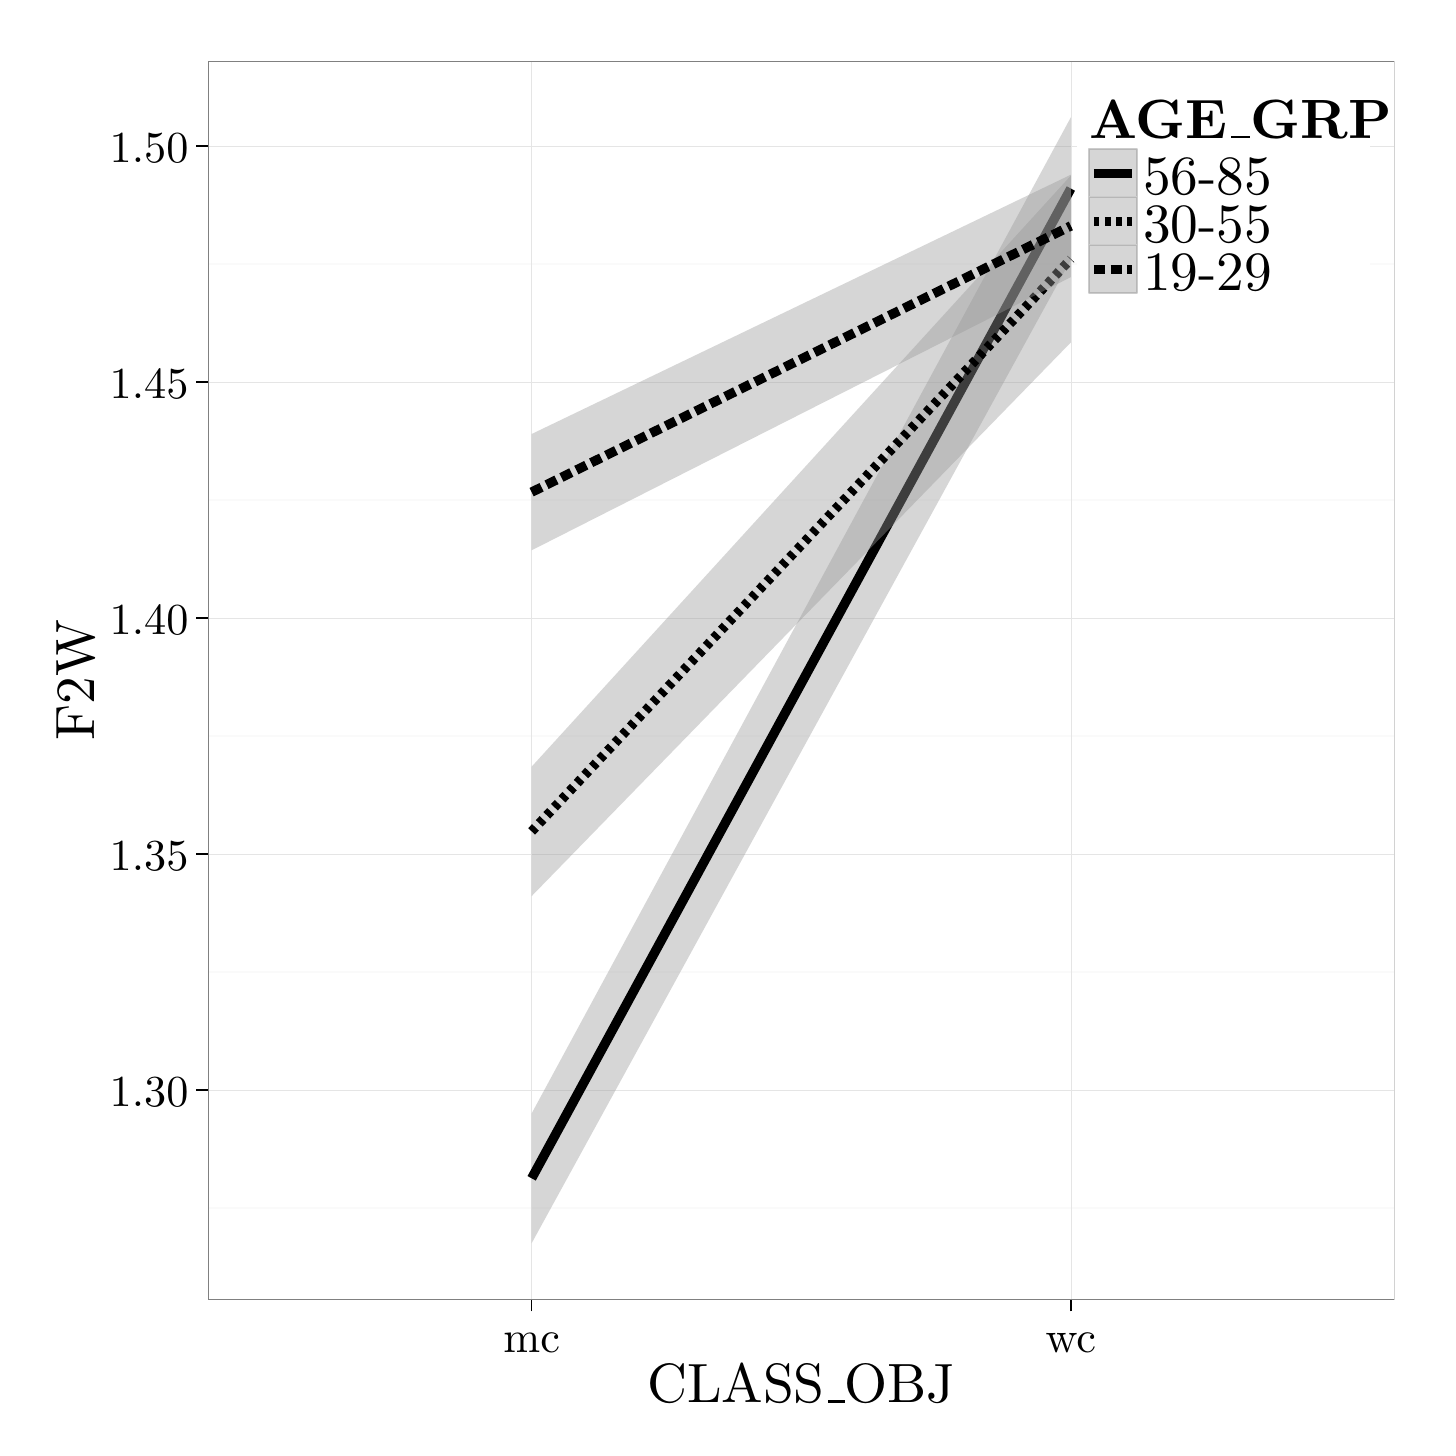
\begin{tikzpicture}[x=1pt,y=1pt]
\definecolor{fillColor}{RGB}{255,255,255}
\path[use as bounding box,fill=fillColor,fill opacity=0.00] (0,0) rectangle (505.89,505.89);
\begin{scope}
\path[clip] (  0.00,  0.00) rectangle (505.89,505.89);
\definecolor{drawColor}{RGB}{255,255,255}
\definecolor{fillColor}{RGB}{255,255,255}

\path[draw=drawColor,line width= 0.6pt,line join=round,line cap=round,fill=fillColor] (  0.00, -0.00) rectangle (505.89,505.89);
\end{scope}
\begin{scope}
\path[clip] ( 65.21, 46.31) rectangle (493.85,493.84);
\definecolor{fillColor}{RGB}{255,255,255}

\path[fill=fillColor] ( 65.21, 46.31) rectangle (493.85,493.84);
\definecolor{drawColor}{gray}{0.98}

\path[draw=drawColor,line width= 0.6pt,line join=round] ( 65.21, 79.40) --
	(493.85, 79.40);

\path[draw=drawColor,line width= 0.6pt,line join=round] ( 65.21,164.68) --
	(493.85,164.68);

\path[draw=drawColor,line width= 0.6pt,line join=round] ( 65.21,249.96) --
	(493.85,249.96);

\path[draw=drawColor,line width= 0.6pt,line join=round] ( 65.21,335.24) --
	(493.85,335.24);

\path[draw=drawColor,line width= 0.6pt,line join=round] ( 65.21,420.52) --
	(493.85,420.52);
\definecolor{drawColor}{gray}{0.90}

\path[draw=drawColor,line width= 0.2pt,line join=round] ( 65.21,122.04) --
	(493.85,122.04);

\path[draw=drawColor,line width= 0.2pt,line join=round] ( 65.21,207.32) --
	(493.85,207.32);

\path[draw=drawColor,line width= 0.2pt,line join=round] ( 65.21,292.60) --
	(493.85,292.60);

\path[draw=drawColor,line width= 0.2pt,line join=round] ( 65.21,377.88) --
	(493.85,377.88);

\path[draw=drawColor,line width= 0.2pt,line join=round] ( 65.21,463.16) --
	(493.85,463.16);

\path[draw=drawColor,line width= 0.2pt,line join=round] (182.11, 46.31) --
	(182.11,493.84);

\path[draw=drawColor,line width= 0.2pt,line join=round] (376.95, 46.31) --
	(376.95,493.84);
\definecolor{fillColor}{RGB}{153,153,153}

\path[fill=fillColor,fill opacity=0.40] (182.11,113.55) --
	(376.95,473.50) --
	(376.95,422.01) --
	(182.11, 66.65) --
	cycle;
\definecolor{drawColor}{RGB}{0,0,0}

\path[draw=drawColor,line width= 3.4pt,line join=round] (182.11, 90.10) --
	(376.95,447.76);

\path[fill=fillColor,fill opacity=0.40] (182.11,238.85) --
	(376.95,452.44) --
	(376.95,392.16) --
	(182.11,192.07) --
	cycle;

\path[draw=drawColor,line width= 3.4pt,dash pattern=on 2pt off 2pt ,line join=round] (182.11,215.46) --
	(376.95,422.30);

\path[fill=fillColor,fill opacity=0.40] (182.11,359.05) --
	(376.95,452.75) --
	(376.95,415.74) --
	(182.11,317.04) --
	cycle;

\path[draw=drawColor,line width= 3.4pt,dash pattern=on 4pt off 2pt ,line join=round] (182.11,338.05) --
	(376.95,434.24);
\definecolor{drawColor}{gray}{0.50}

\path[draw=drawColor,line width= 0.6pt,line join=round,line cap=round] ( 65.21, 46.31) rectangle (493.85,493.84);
\end{scope}
\begin{scope}
\path[clip] (  0.00,  0.00) rectangle (505.89,505.89);
\definecolor{drawColor}{RGB}{0,0,0}

\node[text=drawColor,anchor=base east,inner sep=0pt, outer sep=0pt, scale=  1.60] at ( 58.10,116.01) {1.30};

\node[text=drawColor,anchor=base east,inner sep=0pt, outer sep=0pt, scale=  1.60] at ( 58.10,201.29) {1.35};

\node[text=drawColor,anchor=base east,inner sep=0pt, outer sep=0pt, scale=  1.60] at ( 58.10,286.57) {1.40};

\node[text=drawColor,anchor=base east,inner sep=0pt, outer sep=0pt, scale=  1.60] at ( 58.10,371.85) {1.45};

\node[text=drawColor,anchor=base east,inner sep=0pt, outer sep=0pt, scale=  1.60] at ( 58.10,457.13) {1.50};
\end{scope}
\begin{scope}
\path[clip] (  0.00,  0.00) rectangle (505.89,505.89);
\definecolor{drawColor}{RGB}{0,0,0}

\path[draw=drawColor,line width= 0.6pt,line join=round] ( 60.95,122.04) --
	( 65.21,122.04);

\path[draw=drawColor,line width= 0.6pt,line join=round] ( 60.95,207.32) --
	( 65.21,207.32);

\path[draw=drawColor,line width= 0.6pt,line join=round] ( 60.95,292.60) --
	( 65.21,292.60);

\path[draw=drawColor,line width= 0.6pt,line join=round] ( 60.95,377.88) --
	( 65.21,377.88);

\path[draw=drawColor,line width= 0.6pt,line join=round] ( 60.95,463.16) --
	( 65.21,463.16);
\end{scope}
\begin{scope}
\path[clip] (  0.00,  0.00) rectangle (505.89,505.89);
\definecolor{drawColor}{RGB}{0,0,0}

\path[draw=drawColor,line width= 0.6pt,line join=round] (182.11, 42.04) --
	(182.11, 46.31);

\path[draw=drawColor,line width= 0.6pt,line join=round] (376.95, 42.04) --
	(376.95, 46.31);
\end{scope}
\begin{scope}
\path[clip] (  0.00,  0.00) rectangle (505.89,505.89);
\definecolor{drawColor}{RGB}{0,0,0}

\node[text=drawColor,anchor=base,inner sep=0pt, outer sep=0pt, scale=  1.60] at (182.11, 27.13) {mc};

\node[text=drawColor,anchor=base,inner sep=0pt, outer sep=0pt, scale=  1.60] at (376.95, 27.13) {wc};
\end{scope}
\begin{scope}
\path[clip] (  0.00,  0.00) rectangle (505.89,505.89);
\definecolor{drawColor}{RGB}{0,0,0}

\node[text=drawColor,anchor=base,inner sep=0pt, outer sep=0pt, scale=  2.00] at (279.53,  9.03) {CLASS{\_{}}OBJ};
\end{scope}
\begin{scope}
\path[clip] (  0.00,  0.00) rectangle (505.89,505.89);
\definecolor{drawColor}{RGB}{0,0,0}

\node[text=drawColor,rotate= 90.00,anchor=base,inner sep=0pt, outer sep=0pt, scale=  2.00] at ( 24.12,270.08) {F2W};
\end{scope}
\begin{scope}
\path[clip] (  0.00,  0.00) rectangle (505.89,505.89);
\definecolor{fillColor}{RGB}{255,255,255}

\path[fill=fillColor] (379.28,405.66) rectangle (484.98,484.98);
\end{scope}
\begin{scope}
\path[clip] (  0.00,  0.00) rectangle (505.89,505.89);
\definecolor{drawColor}{RGB}{0,0,0}

\node[text=drawColor,anchor=base west,inner sep=0pt, outer sep=0pt, scale=  2.00] at (383.55,465.96) {\bfseries AGE{\_{}}GRP};
\end{scope}
\begin{scope}
\path[clip] (  0.00,  0.00) rectangle (505.89,505.89);
\definecolor{drawColor}{gray}{0.80}
\definecolor{fillColor}{RGB}{255,255,255}

\path[draw=drawColor,line width= 0.6pt,line join=round,line cap=round,fill=fillColor] (383.55,444.61) rectangle (400.89,461.96);
\end{scope}
\begin{scope}
\path[clip] (  0.00,  0.00) rectangle (505.89,505.89);
\definecolor{fillColor}{RGB}{153,153,153}

\path[fill=fillColor,fill opacity=0.40] (383.55,444.61) rectangle (400.89,461.96);
\definecolor{drawColor}{RGB}{0,0,0}

\path[draw=drawColor,line width= 3.4pt,line join=round] (385.28,453.29) -- (399.16,453.29);
\end{scope}
\begin{scope}
\path[clip] (  0.00,  0.00) rectangle (505.89,505.89);
\definecolor{drawColor}{gray}{0.80}
\definecolor{fillColor}{RGB}{255,255,255}

\path[draw=drawColor,line width= 0.6pt,line join=round,line cap=round,fill=fillColor] (383.55,427.27) rectangle (400.89,444.61);
\end{scope}
\begin{scope}
\path[clip] (  0.00,  0.00) rectangle (505.89,505.89);
\definecolor{fillColor}{RGB}{153,153,153}

\path[fill=fillColor,fill opacity=0.40] (383.55,427.27) rectangle (400.89,444.61);
\definecolor{drawColor}{RGB}{0,0,0}

\path[draw=drawColor,line width= 3.4pt,dash pattern=on 2pt off 2pt ,line join=round] (385.28,435.94) -- (399.16,435.94);
\end{scope}
\begin{scope}
\path[clip] (  0.00,  0.00) rectangle (505.89,505.89);
\definecolor{drawColor}{gray}{0.80}
\definecolor{fillColor}{RGB}{255,255,255}

\path[draw=drawColor,line width= 0.6pt,line join=round,line cap=round,fill=fillColor] (383.55,409.92) rectangle (400.89,427.27);
\end{scope}
\begin{scope}
\path[clip] (  0.00,  0.00) rectangle (505.89,505.89);
\definecolor{fillColor}{RGB}{153,153,153}

\path[fill=fillColor,fill opacity=0.40] (383.55,409.92) rectangle (400.89,427.27);
\definecolor{drawColor}{RGB}{0,0,0}

\path[draw=drawColor,line width= 3.4pt,dash pattern=on 4pt off 2pt ,line join=round] (385.28,418.60) -- (399.16,418.60);
\end{scope}
\begin{scope}
\path[clip] (  0.00,  0.00) rectangle (505.89,505.89);
\definecolor{drawColor}{RGB}{0,0,0}

\node[text=drawColor,anchor=base west,inner sep=0pt, outer sep=0pt, scale=  2.00] at (403.06,445.75) {56-85};
\end{scope}
\begin{scope}
\path[clip] (  0.00,  0.00) rectangle (505.89,505.89);
\definecolor{drawColor}{RGB}{0,0,0}

\node[text=drawColor,anchor=base west,inner sep=0pt, outer sep=0pt, scale=  2.00] at (403.06,428.40) {30-55};
\end{scope}
\begin{scope}
\path[clip] (  0.00,  0.00) rectangle (505.89,505.89);
\definecolor{drawColor}{RGB}{0,0,0}

\node[text=drawColor,anchor=base west,inner sep=0pt, outer sep=0pt, scale=  2.00] at (403.06,411.06) {19-29};
\end{scope}
\end{tikzpicture}
} 
		\caption{regression plot}
		\label{fig.scatter.f2w.nurse.ageclass}
	\end{subfigure}
	\caption{\textsc{nurse} (F2) by age and class}
\end{figure}

When we look at class differences in the three age groups separately, we arrive at the picture represented by the box plots in Figure \ref{fig.box.f2w.nurse.ageclass}.
In all three groups, the means of middle-class speakers are lower than that of the working-class interviewees.
For the oldest speakers (left panel) the difference is particularly pronounced.
Both means and medians are different in a statistically robust way: the interquartile ranges of the two boxes do not overlap, and a t-test also finds this difference to be significant (t(362.001) = -19.881, p < 0.001).
In the middle group there is a greater amount of variation (both boxes are larger) and both means and medians are closer to each other.
As a consequence, the interquartile ranges do overlap, but middle-class and working-class speakers do all the same differ in a highly significant way in this age group as well (t(615.171) = -10.466, p < 0.001).
When the dataset is restricted to the youngest speakers the difference between social classes is further reduced.
At the same time values are more homogeneous in this age group --- visually represented by the vertical extent of the boxes, which is smaller than in the middle group and comparable to the one found for the oldest speakers.
While less pronounced, the difference between middle and working-class speakers is therefore just as significant for the youngest subjects as it is in the other groups (t(521.157) = -6.815, p < 0.001).

\begin{table}[h!]
	\centering
	\caption{\textsc{nurse} (F2): t-tests of age by social class}
	\label{tab.nurse.f2.classage.pvalues}
	\begin{tabular}{lrrrrrr}
		\hline
		test & \multicolumn{3}{c}{middle class} & \multicolumn{3}{c}{working class}\\
		& t & df & p & t & df & p\\
		\hline
		old-middle & 7.842 & 645.309 & < 0.001 & \ensuremath{-1.189} & 482.408 & 0.235\\
		middle-young & 7.920 & 698.035 & < 0.001 & 0.638 & 507.159 & 0.524\\
		young-old & 16.507 & 452.539 & < 0.001 & \ensuremath{-0.784} & 349.296 & 0.434\\			 
		\hline
	\end{tabular}
\end{table}

Figure \ref{fig.box.f2w.nurse.ageclass} also shows that it is due to the middle-class speakers that the social class difference decreases linearly from the oldest to the youngest speakers.
Working-class realisations are, in fact, remarkably stable over the three generations investigated here.
For middle-class speakers, on the other hand, \textsc{nurse} variants become consistently fronter from the oldest to the youngest speakers.
In Figure \ref{fig.scatter.f2w.nurse.ageclass}, the decreasing distance between social classes is visible in the slopes of the regression lines, which become flatter from the old (solid) to the middle-aged (dotted) and young speakers (dashed).
This graph also provides support for the other point made above.
For middle-class speakers (on the left-hand side of Figure \ref{fig.scatter.f2w.nurse.ageclass}), all three age groups are different from each other (cf. the three relevant t-tests in Table \ref{tab.nurse.f2.classage.pvalues}, which all yielded significant results).
In the working-class sub-sample, all regression lines occupy essentially the same place, and all standard deviations overlap (dark grey area).
T-tests on the raw data (cf. again Table \ref{tab.nurse.f2.classage.pvalues}) also confirm the claim voiced above that age differences only exist in the working, but not the middle class.

\subsubsection{Style shifting}
\label{sec.prod.res.vow.nurse.f2.shifting}

\begin{figure}[h!]
	\centering
		\definecolor{shadecolor}{rgb}{0.969, 0.969, 0.969}
		\resizebox{0.5\linewidth}{!}{% Created by tikzDevice version 0.8.1 on 2016-02-09 02:15:16
% !TEX encoding = UTF-8 Unicode
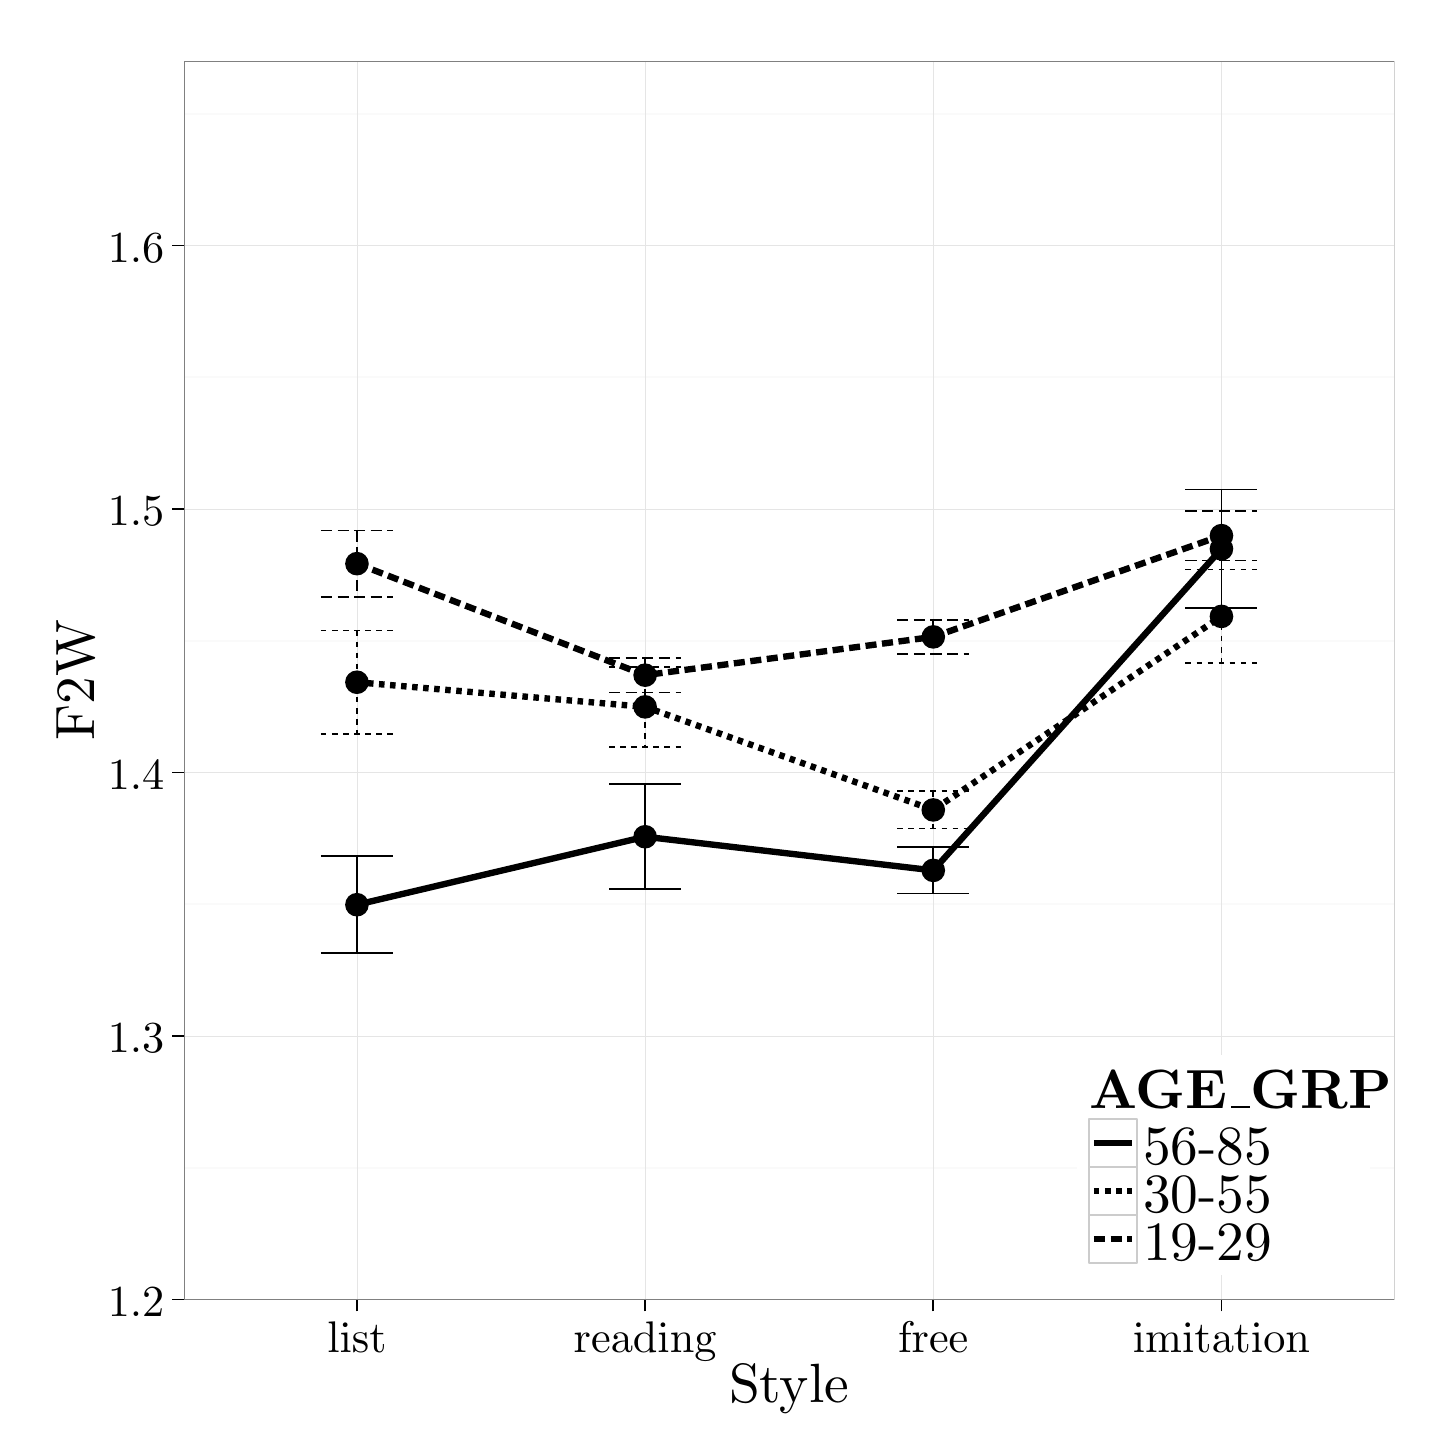
\begin{tikzpicture}[x=1pt,y=1pt]
\definecolor{fillColor}{RGB}{255,255,255}
\path[use as bounding box,fill=fillColor,fill opacity=0.00] (0,0) rectangle (505.89,505.89);
\begin{scope}
\path[clip] (  0.00,  0.00) rectangle (505.89,505.89);
\definecolor{drawColor}{RGB}{255,255,255}
\definecolor{fillColor}{RGB}{255,255,255}

\path[draw=drawColor,line width= 0.6pt,line join=round,line cap=round,fill=fillColor] (  0.00, -0.00) rectangle (505.89,505.89);
\end{scope}
\begin{scope}
\path[clip] ( 56.50, 46.31) rectangle (493.85,493.84);
\definecolor{fillColor}{RGB}{255,255,255}

\path[fill=fillColor] ( 56.50, 46.31) rectangle (493.85,493.84);
\definecolor{drawColor}{gray}{0.98}

\path[draw=drawColor,line width= 0.6pt,line join=round] ( 56.50, 93.92) --
	(493.85, 93.92);

\path[draw=drawColor,line width= 0.6pt,line join=round] ( 56.50,189.14) --
	(493.85,189.14);

\path[draw=drawColor,line width= 0.6pt,line join=round] ( 56.50,284.36) --
	(493.85,284.36);

\path[draw=drawColor,line width= 0.6pt,line join=round] ( 56.50,379.58) --
	(493.85,379.58);

\path[draw=drawColor,line width= 0.6pt,line join=round] ( 56.50,474.80) --
	(493.85,474.80);
\definecolor{drawColor}{gray}{0.90}

\path[draw=drawColor,line width= 0.2pt,line join=round] ( 56.50, 46.31) --
	(493.85, 46.31);

\path[draw=drawColor,line width= 0.2pt,line join=round] ( 56.50,141.53) --
	(493.85,141.53);

\path[draw=drawColor,line width= 0.2pt,line join=round] ( 56.50,236.75) --
	(493.85,236.75);

\path[draw=drawColor,line width= 0.2pt,line join=round] ( 56.50,331.97) --
	(493.85,331.97);

\path[draw=drawColor,line width= 0.2pt,line join=round] ( 56.50,427.19) --
	(493.85,427.19);

\path[draw=drawColor,line width= 0.2pt,line join=round] (118.98, 46.31) --
	(118.98,493.84);

\path[draw=drawColor,line width= 0.2pt,line join=round] (223.11, 46.31) --
	(223.11,493.84);

\path[draw=drawColor,line width= 0.2pt,line join=round] (327.24, 46.31) --
	(327.24,493.84);

\path[draw=drawColor,line width= 0.2pt,line join=round] (431.37, 46.31) --
	(431.37,493.84);
\definecolor{fillColor}{RGB}{0,0,0}

\path[fill=fillColor] (118.98,188.97) circle (  4.27);

\path[fill=fillColor] (118.98,269.36) circle (  4.27);

\path[fill=fillColor] (118.98,312.21) circle (  4.27);

\path[fill=fillColor] (223.11,213.53) circle (  4.27);

\path[fill=fillColor] (223.11,260.46) circle (  4.27);

\path[fill=fillColor] (223.11,271.91) circle (  4.27);

\path[fill=fillColor] (327.24,201.37) circle (  4.27);

\path[fill=fillColor] (327.24,223.22) circle (  4.27);

\path[fill=fillColor] (327.24,285.75) circle (  4.27);

\path[fill=fillColor] (431.37,317.56) circle (  4.27);

\path[fill=fillColor] (431.37,293.15) circle (  4.27);

\path[fill=fillColor] (431.37,322.33) circle (  4.27);
\definecolor{drawColor}{RGB}{0,0,0}

\path[draw=drawColor,line width= 2.3pt,line join=round] (118.98,188.97) --
	(223.11,213.53) --
	(327.24,201.37) --
	(431.37,317.56);

\path[draw=drawColor,line width= 2.3pt,dash pattern=on 2pt off 2pt ,line join=round] (118.98,269.36) --
	(223.11,260.46) --
	(327.24,223.22) --
	(431.37,293.15);

\path[draw=drawColor,line width= 2.3pt,dash pattern=on 4pt off 2pt ,line join=round] (118.98,312.21) --
	(223.11,271.91) --
	(327.24,285.75) --
	(431.37,322.33);

\path[draw=drawColor,line width= 0.6pt,line join=round] (105.96,206.49) --
	(132.00,206.49);

\path[draw=drawColor,line width= 0.6pt,line join=round] (118.98,206.49) --
	(118.98,171.45);

\path[draw=drawColor,line width= 0.6pt,line join=round] (105.96,171.45) --
	(132.00,171.45);

\path[draw=drawColor,line width= 0.6pt,line join=round] (210.09,232.48) --
	(236.13,232.48);

\path[draw=drawColor,line width= 0.6pt,line join=round] (223.11,232.48) --
	(223.11,194.58);

\path[draw=drawColor,line width= 0.6pt,line join=round] (210.09,194.58) --
	(236.13,194.58);

\path[draw=drawColor,line width= 0.6pt,line join=round] (314.22,209.77) --
	(340.25,209.77);

\path[draw=drawColor,line width= 0.6pt,line join=round] (327.24,209.77) --
	(327.24,192.97);

\path[draw=drawColor,line width= 0.6pt,line join=round] (314.22,192.97) --
	(340.25,192.97);

\path[draw=drawColor,line width= 0.6pt,line join=round] (418.35,338.99) --
	(444.38,338.99);

\path[draw=drawColor,line width= 0.6pt,line join=round] (431.37,338.99) --
	(431.37,296.12);

\path[draw=drawColor,line width= 0.6pt,line join=round] (418.35,296.12) --
	(444.38,296.12);

\path[draw=drawColor,line width= 0.6pt,dash pattern=on 2pt off 2pt ,line join=round] (105.96,288.05) --
	(132.00,288.05);

\path[draw=drawColor,line width= 0.6pt,dash pattern=on 2pt off 2pt ,line join=round] (118.98,288.05) --
	(118.98,250.67);

\path[draw=drawColor,line width= 0.6pt,dash pattern=on 2pt off 2pt ,line join=round] (105.96,250.67) --
	(132.00,250.67);

\path[draw=drawColor,line width= 0.6pt,dash pattern=on 2pt off 2pt ,line join=round] (210.09,274.85) --
	(236.13,274.85);

\path[draw=drawColor,line width= 0.6pt,dash pattern=on 2pt off 2pt ,line join=round] (223.11,274.85) --
	(223.11,246.07);

\path[draw=drawColor,line width= 0.6pt,dash pattern=on 2pt off 2pt ,line join=round] (210.09,246.07) --
	(236.13,246.07);

\path[draw=drawColor,line width= 0.6pt,dash pattern=on 2pt off 2pt ,line join=round] (314.22,229.99) --
	(340.25,229.99);

\path[draw=drawColor,line width= 0.6pt,dash pattern=on 2pt off 2pt ,line join=round] (327.24,229.99) --
	(327.24,216.45);

\path[draw=drawColor,line width= 0.6pt,dash pattern=on 2pt off 2pt ,line join=round] (314.22,216.45) --
	(340.25,216.45);

\path[draw=drawColor,line width= 0.6pt,dash pattern=on 2pt off 2pt ,line join=round] (418.35,310.08) --
	(444.38,310.08);

\path[draw=drawColor,line width= 0.6pt,dash pattern=on 2pt off 2pt ,line join=round] (431.37,310.08) --
	(431.37,276.22);

\path[draw=drawColor,line width= 0.6pt,dash pattern=on 2pt off 2pt ,line join=round] (418.35,276.22) --
	(444.38,276.22);

\path[draw=drawColor,line width= 0.6pt,dash pattern=on 4pt off 2pt ,line join=round] (105.96,324.19) --
	(132.00,324.19);

\path[draw=drawColor,line width= 0.6pt,dash pattern=on 4pt off 2pt ,line join=round] (118.98,324.19) --
	(118.98,300.22);

\path[draw=drawColor,line width= 0.6pt,dash pattern=on 4pt off 2pt ,line join=round] (105.96,300.22) --
	(132.00,300.22);

\path[draw=drawColor,line width= 0.6pt,dash pattern=on 4pt off 2pt ,line join=round] (210.09,278.22) --
	(236.13,278.22);

\path[draw=drawColor,line width= 0.6pt,dash pattern=on 4pt off 2pt ,line join=round] (223.11,278.22) --
	(223.11,265.61);

\path[draw=drawColor,line width= 0.6pt,dash pattern=on 4pt off 2pt ,line join=round] (210.09,265.61) --
	(236.13,265.61);

\path[draw=drawColor,line width= 0.6pt,dash pattern=on 4pt off 2pt ,line join=round] (314.22,291.91) --
	(340.25,291.91);

\path[draw=drawColor,line width= 0.6pt,dash pattern=on 4pt off 2pt ,line join=round] (327.24,291.91) --
	(327.24,279.59);

\path[draw=drawColor,line width= 0.6pt,dash pattern=on 4pt off 2pt ,line join=round] (314.22,279.59) --
	(340.25,279.59);

\path[draw=drawColor,line width= 0.6pt,dash pattern=on 4pt off 2pt ,line join=round] (418.35,331.27) --
	(444.38,331.27);

\path[draw=drawColor,line width= 0.6pt,dash pattern=on 4pt off 2pt ,line join=round] (431.37,331.27) --
	(431.37,313.39);

\path[draw=drawColor,line width= 0.6pt,dash pattern=on 4pt off 2pt ,line join=round] (418.35,313.39) --
	(444.38,313.39);
\definecolor{drawColor}{gray}{0.50}

\path[draw=drawColor,line width= 0.6pt,line join=round,line cap=round] ( 56.50, 46.31) rectangle (493.85,493.84);
\end{scope}
\begin{scope}
\path[clip] (  0.00,  0.00) rectangle (505.89,505.89);
\definecolor{drawColor}{RGB}{0,0,0}

\node[text=drawColor,anchor=base east,inner sep=0pt, outer sep=0pt, scale=  1.60] at ( 49.39, 40.27) {1.2};

\node[text=drawColor,anchor=base east,inner sep=0pt, outer sep=0pt, scale=  1.60] at ( 49.39,135.50) {1.3};

\node[text=drawColor,anchor=base east,inner sep=0pt, outer sep=0pt, scale=  1.60] at ( 49.39,230.72) {1.4};

\node[text=drawColor,anchor=base east,inner sep=0pt, outer sep=0pt, scale=  1.60] at ( 49.39,325.94) {1.5};

\node[text=drawColor,anchor=base east,inner sep=0pt, outer sep=0pt, scale=  1.60] at ( 49.39,421.16) {1.6};
\end{scope}
\begin{scope}
\path[clip] (  0.00,  0.00) rectangle (505.89,505.89);
\definecolor{drawColor}{RGB}{0,0,0}

\path[draw=drawColor,line width= 0.6pt,line join=round] ( 52.24, 46.31) --
	( 56.50, 46.31);

\path[draw=drawColor,line width= 0.6pt,line join=round] ( 52.24,141.53) --
	( 56.50,141.53);

\path[draw=drawColor,line width= 0.6pt,line join=round] ( 52.24,236.75) --
	( 56.50,236.75);

\path[draw=drawColor,line width= 0.6pt,line join=round] ( 52.24,331.97) --
	( 56.50,331.97);

\path[draw=drawColor,line width= 0.6pt,line join=round] ( 52.24,427.19) --
	( 56.50,427.19);
\end{scope}
\begin{scope}
\path[clip] (  0.00,  0.00) rectangle (505.89,505.89);
\definecolor{drawColor}{RGB}{0,0,0}

\path[draw=drawColor,line width= 0.6pt,line join=round] (118.98, 42.04) --
	(118.98, 46.31);

\path[draw=drawColor,line width= 0.6pt,line join=round] (223.11, 42.04) --
	(223.11, 46.31);

\path[draw=drawColor,line width= 0.6pt,line join=round] (327.24, 42.04) --
	(327.24, 46.31);

\path[draw=drawColor,line width= 0.6pt,line join=round] (431.37, 42.04) --
	(431.37, 46.31);
\end{scope}
\begin{scope}
\path[clip] (  0.00,  0.00) rectangle (505.89,505.89);
\definecolor{drawColor}{RGB}{0,0,0}

\node[text=drawColor,anchor=base,inner sep=0pt, outer sep=0pt, scale=  1.60] at (118.98, 27.13) {list};

\node[text=drawColor,anchor=base,inner sep=0pt, outer sep=0pt, scale=  1.60] at (223.11, 27.13) {reading};

\node[text=drawColor,anchor=base,inner sep=0pt, outer sep=0pt, scale=  1.60] at (327.24, 27.13) {free};

\node[text=drawColor,anchor=base,inner sep=0pt, outer sep=0pt, scale=  1.60] at (431.37, 27.13) {imitation};
\end{scope}
\begin{scope}
\path[clip] (  0.00,  0.00) rectangle (505.89,505.89);
\definecolor{drawColor}{RGB}{0,0,0}

\node[text=drawColor,anchor=base,inner sep=0pt, outer sep=0pt, scale=  2.00] at (275.17,  9.03) {Style};
\end{scope}
\begin{scope}
\path[clip] (  0.00,  0.00) rectangle (505.89,505.89);
\definecolor{drawColor}{RGB}{0,0,0}

\node[text=drawColor,rotate= 90.00,anchor=base,inner sep=0pt, outer sep=0pt, scale=  2.00] at ( 24.12,270.08) {F2W};
\end{scope}
\begin{scope}
\path[clip] (  0.00,  0.00) rectangle (505.89,505.89);
\definecolor{fillColor}{RGB}{255,255,255}

\path[fill=fillColor] (379.28, 55.18) rectangle (484.98,134.50);
\end{scope}
\begin{scope}
\path[clip] (  0.00,  0.00) rectangle (505.89,505.89);
\definecolor{drawColor}{RGB}{0,0,0}

\node[text=drawColor,anchor=base west,inner sep=0pt, outer sep=0pt, scale=  2.00] at (383.55,115.48) {\bfseries AGE{\_{}}GRP};
\end{scope}
\begin{scope}
\path[clip] (  0.00,  0.00) rectangle (505.89,505.89);
\definecolor{drawColor}{gray}{0.80}
\definecolor{fillColor}{RGB}{255,255,255}

\path[draw=drawColor,line width= 0.6pt,line join=round,line cap=round,fill=fillColor] (383.55, 94.13) rectangle (400.89,111.48);
\end{scope}
\begin{scope}
\path[clip] (  0.00,  0.00) rectangle (505.89,505.89);
\definecolor{drawColor}{RGB}{0,0,0}

\path[draw=drawColor,line width= 2.3pt,line join=round] (385.28,102.81) -- (399.16,102.81);
\end{scope}
\begin{scope}
\path[clip] (  0.00,  0.00) rectangle (505.89,505.89);
\definecolor{drawColor}{RGB}{0,0,0}

\path[draw=drawColor,line width= 0.6pt,line join=round] (385.28,102.81) -- (399.16,102.81);
\end{scope}
\begin{scope}
\path[clip] (  0.00,  0.00) rectangle (505.89,505.89);
\definecolor{drawColor}{gray}{0.80}
\definecolor{fillColor}{RGB}{255,255,255}

\path[draw=drawColor,line width= 0.6pt,line join=round,line cap=round,fill=fillColor] (383.55, 76.79) rectangle (400.89, 94.13);
\end{scope}
\begin{scope}
\path[clip] (  0.00,  0.00) rectangle (505.89,505.89);
\definecolor{drawColor}{RGB}{0,0,0}

\path[draw=drawColor,line width= 2.3pt,dash pattern=on 2pt off 2pt ,line join=round] (385.28, 85.46) -- (399.16, 85.46);
\end{scope}
\begin{scope}
\path[clip] (  0.00,  0.00) rectangle (505.89,505.89);
\definecolor{drawColor}{RGB}{0,0,0}

\path[draw=drawColor,line width= 0.6pt,dash pattern=on 2pt off 2pt ,line join=round] (385.28, 85.46) -- (399.16, 85.46);
\end{scope}
\begin{scope}
\path[clip] (  0.00,  0.00) rectangle (505.89,505.89);
\definecolor{drawColor}{gray}{0.80}
\definecolor{fillColor}{RGB}{255,255,255}

\path[draw=drawColor,line width= 0.6pt,line join=round,line cap=round,fill=fillColor] (383.55, 59.44) rectangle (400.89, 76.79);
\end{scope}
\begin{scope}
\path[clip] (  0.00,  0.00) rectangle (505.89,505.89);
\definecolor{drawColor}{RGB}{0,0,0}

\path[draw=drawColor,line width= 2.3pt,dash pattern=on 4pt off 2pt ,line join=round] (385.28, 68.12) -- (399.16, 68.12);
\end{scope}
\begin{scope}
\path[clip] (  0.00,  0.00) rectangle (505.89,505.89);
\definecolor{drawColor}{RGB}{0,0,0}

\path[draw=drawColor,line width= 0.6pt,dash pattern=on 4pt off 2pt ,line join=round] (385.28, 68.12) -- (399.16, 68.12);
\end{scope}
\begin{scope}
\path[clip] (  0.00,  0.00) rectangle (505.89,505.89);
\definecolor{drawColor}{RGB}{0,0,0}

\node[text=drawColor,anchor=base west,inner sep=0pt, outer sep=0pt, scale=  2.00] at (403.06, 95.26) {56-85};
\end{scope}
\begin{scope}
\path[clip] (  0.00,  0.00) rectangle (505.89,505.89);
\definecolor{drawColor}{RGB}{0,0,0}

\node[text=drawColor,anchor=base west,inner sep=0pt, outer sep=0pt, scale=  2.00] at (403.06, 77.92) {30-55};
\end{scope}
\begin{scope}
\path[clip] (  0.00,  0.00) rectangle (505.89,505.89);
\definecolor{drawColor}{RGB}{0,0,0}

\node[text=drawColor,anchor=base west,inner sep=0pt, outer sep=0pt, scale=  2.00] at (403.06, 60.57) {19-29};
\end{scope}
\end{tikzpicture}
} 
	\caption{\textsc{nurse} (F2) by style and age}
	\label{fig.line.f2.nurse.tot}
\end{figure}

The last combinations of predictors that can tell us something about the (\isi{change} in) \isi{salience} of \textsc{nurse} are the two-way interaction of style and age, and the three-way interaction of style, age, and social class.
The relationship of style and age of participant is visualised in Figure \ref{fig.line.f2.nurse.tot}.
For the oldest group (solid line) there seems to be some movement from the word list to the reading passage to spontaneous speech, but in fact the standard error whiskers indicate that, statistically speaking, these three styles have identical \textsc{nurse} realisations.
Only the extreme rise when actively perform\is{accent performance}ing Scouse results in a mean that is significantly different from the other three registers.
This sharp increase in F2 values from free speech to accent imitation\is{accent performance} is also present (and just as significant) in the middle-aged group.
Spontaneous realisations in this age group are also significantly different from the `reading' register, but, interestingly, \textsc{nurse} is \emph{fronter} --- more Scouse --- in this more formal register.
The same goes for the word list, a register which is not significantly different from reading for these subjects.
F2 values in the middle age group thus strongly hint at hypercorrect\is{hypercorrection}ion (cf. Section \ref{sec.prod.res.vow.nurse.pil}).
Speakers in the young group, finally, exhibit a pattern which is closest to what we would expect if we assume there to be \isi{style shifting}: F2 increases from reading a text to free speech and from spontaneous speech to accent imitation\is{accent performance}; both these increases are (just about in the former case) statistically robust.
The only thing that does not fit into this frame is that realisations when reading out the word list are actually just as front as when these speakers imitate a particularly strong Scouse accent (no significant difference).
In the most formal register young speakers' behaviour is therefore opposite to what would be expected.

\begin{figure}[h!]
	\centering
	\begin{subfigure}{.49\textwidth}
		\centering
			\definecolor{shadecolor}{rgb}{0.969, 0.969, 0.969}
			\resizebox{\linewidth}{!}{% Created by tikzDevice version 0.8.1 on 2016-02-09 02:15:16
% !TEX encoding = UTF-8 Unicode
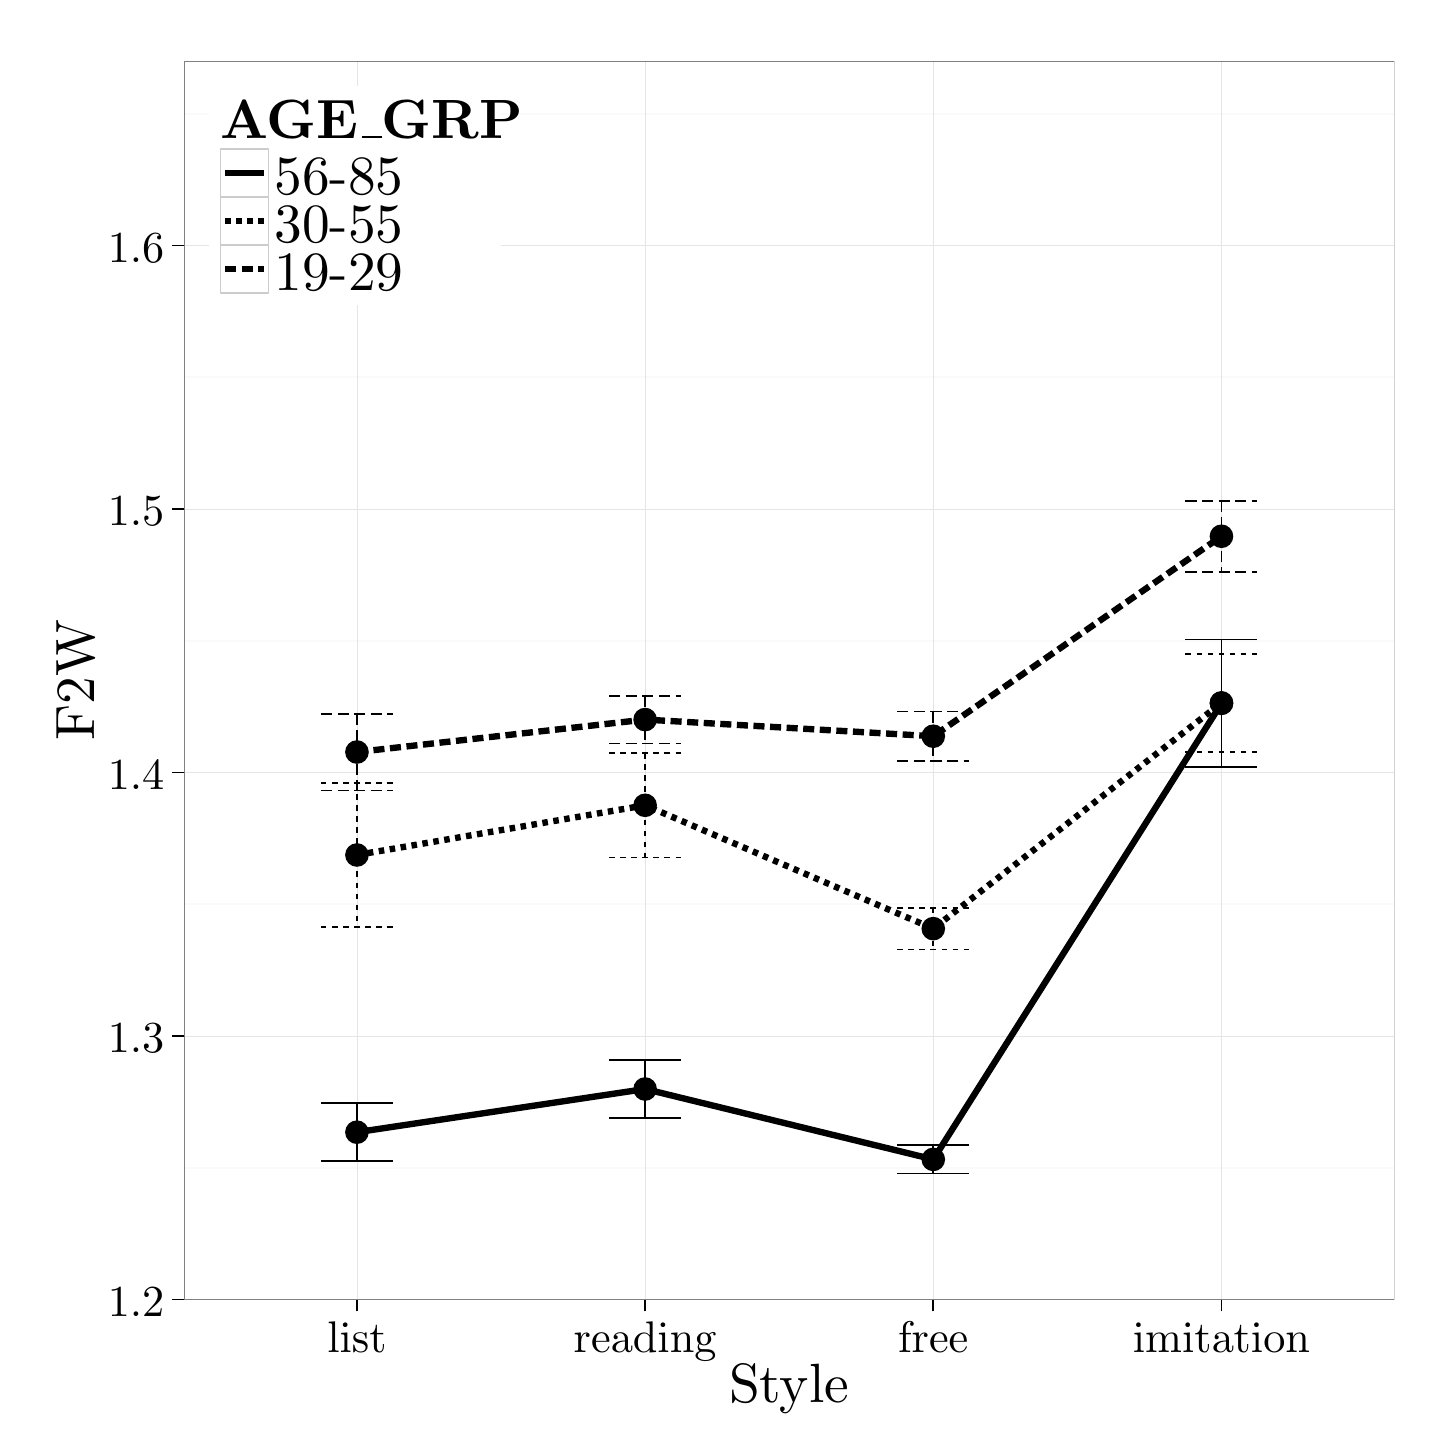
\begin{tikzpicture}[x=1pt,y=1pt]
\definecolor{fillColor}{RGB}{255,255,255}
\path[use as bounding box,fill=fillColor,fill opacity=0.00] (0,0) rectangle (505.89,505.89);
\begin{scope}
\path[clip] (  0.00,  0.00) rectangle (505.89,505.89);
\definecolor{drawColor}{RGB}{255,255,255}
\definecolor{fillColor}{RGB}{255,255,255}

\path[draw=drawColor,line width= 0.6pt,line join=round,line cap=round,fill=fillColor] (  0.00, -0.00) rectangle (505.89,505.89);
\end{scope}
\begin{scope}
\path[clip] ( 56.50, 46.31) rectangle (493.85,493.84);
\definecolor{fillColor}{RGB}{255,255,255}

\path[fill=fillColor] ( 56.50, 46.31) rectangle (493.85,493.84);
\definecolor{drawColor}{gray}{0.98}

\path[draw=drawColor,line width= 0.6pt,line join=round] ( 56.50, 93.92) --
	(493.85, 93.92);

\path[draw=drawColor,line width= 0.6pt,line join=round] ( 56.50,189.14) --
	(493.85,189.14);

\path[draw=drawColor,line width= 0.6pt,line join=round] ( 56.50,284.36) --
	(493.85,284.36);

\path[draw=drawColor,line width= 0.6pt,line join=round] ( 56.50,379.58) --
	(493.85,379.58);

\path[draw=drawColor,line width= 0.6pt,line join=round] ( 56.50,474.80) --
	(493.85,474.80);
\definecolor{drawColor}{gray}{0.90}

\path[draw=drawColor,line width= 0.2pt,line join=round] ( 56.50, 46.31) --
	(493.85, 46.31);

\path[draw=drawColor,line width= 0.2pt,line join=round] ( 56.50,141.53) --
	(493.85,141.53);

\path[draw=drawColor,line width= 0.2pt,line join=round] ( 56.50,236.75) --
	(493.85,236.75);

\path[draw=drawColor,line width= 0.2pt,line join=round] ( 56.50,331.97) --
	(493.85,331.97);

\path[draw=drawColor,line width= 0.2pt,line join=round] ( 56.50,427.19) --
	(493.85,427.19);

\path[draw=drawColor,line width= 0.2pt,line join=round] (118.98, 46.31) --
	(118.98,493.84);

\path[draw=drawColor,line width= 0.2pt,line join=round] (223.11, 46.31) --
	(223.11,493.84);

\path[draw=drawColor,line width= 0.2pt,line join=round] (327.24, 46.31) --
	(327.24,493.84);

\path[draw=drawColor,line width= 0.2pt,line join=round] (431.37, 46.31) --
	(431.37,493.84);
\definecolor{fillColor}{RGB}{0,0,0}

\path[fill=fillColor] (118.98,106.77) circle (  4.27);

\path[fill=fillColor] (118.98,206.94) circle (  4.27);

\path[fill=fillColor] (118.98,244.14) circle (  4.27);

\path[fill=fillColor] (223.11,122.37) circle (  4.27);

\path[fill=fillColor] (223.11,224.89) circle (  4.27);

\path[fill=fillColor] (223.11,255.87) circle (  4.27);

\path[fill=fillColor] (327.24, 96.94) circle (  4.27);

\path[fill=fillColor] (327.24,180.32) circle (  4.27);

\path[fill=fillColor] (327.24,249.85) circle (  4.27);

\path[fill=fillColor] (431.37,261.72) circle (  4.27);

\path[fill=fillColor] (431.37,261.91) circle (  4.27);

\path[fill=fillColor] (431.37,322.11) circle (  4.27);
\definecolor{drawColor}{RGB}{0,0,0}

\path[draw=drawColor,line width= 2.3pt,line join=round] (118.98,106.77) --
	(223.11,122.37) --
	(327.24, 96.94) --
	(431.37,261.72);

\path[draw=drawColor,line width= 2.3pt,dash pattern=on 2pt off 2pt ,line join=round] (118.98,206.94) --
	(223.11,224.89) --
	(327.24,180.32) --
	(431.37,261.91);

\path[draw=drawColor,line width= 2.3pt,dash pattern=on 4pt off 2pt ,line join=round] (118.98,244.14) --
	(223.11,255.87) --
	(327.24,249.85) --
	(431.37,322.11);

\path[draw=drawColor,line width= 0.6pt,line join=round] (105.96,117.25) --
	(132.00,117.25);

\path[draw=drawColor,line width= 0.6pt,line join=round] (118.98,117.25) --
	(118.98, 96.30);

\path[draw=drawColor,line width= 0.6pt,line join=round] (105.96, 96.30) --
	(132.00, 96.30);

\path[draw=drawColor,line width= 0.6pt,line join=round] (210.09,132.83) --
	(236.13,132.83);

\path[draw=drawColor,line width= 0.6pt,line join=round] (223.11,132.83) --
	(223.11,111.92);

\path[draw=drawColor,line width= 0.6pt,line join=round] (210.09,111.92) --
	(236.13,111.92);

\path[draw=drawColor,line width= 0.6pt,line join=round] (314.22,102.07) --
	(340.25,102.07);

\path[draw=drawColor,line width= 0.6pt,line join=round] (327.24,102.07) --
	(327.24, 91.82);

\path[draw=drawColor,line width= 0.6pt,line join=round] (314.22, 91.82) --
	(340.25, 91.82);

\path[draw=drawColor,line width= 0.6pt,line join=round] (418.35,284.76) --
	(444.38,284.76);

\path[draw=drawColor,line width= 0.6pt,line join=round] (431.37,284.76) --
	(431.37,238.69);

\path[draw=drawColor,line width= 0.6pt,line join=round] (418.35,238.69) --
	(444.38,238.69);

\path[draw=drawColor,line width= 0.6pt,dash pattern=on 2pt off 2pt ,line join=round] (105.96,232.98) --
	(132.00,232.98);

\path[draw=drawColor,line width= 0.6pt,dash pattern=on 2pt off 2pt ,line join=round] (118.98,232.98) --
	(118.98,180.91);

\path[draw=drawColor,line width= 0.6pt,dash pattern=on 2pt off 2pt ,line join=round] (105.96,180.91) --
	(132.00,180.91);

\path[draw=drawColor,line width= 0.6pt,dash pattern=on 2pt off 2pt ,line join=round] (210.09,243.69) --
	(236.13,243.69);

\path[draw=drawColor,line width= 0.6pt,dash pattern=on 2pt off 2pt ,line join=round] (223.11,243.69) --
	(223.11,206.09);

\path[draw=drawColor,line width= 0.6pt,dash pattern=on 2pt off 2pt ,line join=round] (210.09,206.09) --
	(236.13,206.09);

\path[draw=drawColor,line width= 0.6pt,dash pattern=on 2pt off 2pt ,line join=round] (314.22,187.88) --
	(340.25,187.88);

\path[draw=drawColor,line width= 0.6pt,dash pattern=on 2pt off 2pt ,line join=round] (327.24,187.88) --
	(327.24,172.76);

\path[draw=drawColor,line width= 0.6pt,dash pattern=on 2pt off 2pt ,line join=round] (314.22,172.76) --
	(340.25,172.76);

\path[draw=drawColor,line width= 0.6pt,dash pattern=on 2pt off 2pt ,line join=round] (418.35,279.57) --
	(444.38,279.57);

\path[draw=drawColor,line width= 0.6pt,dash pattern=on 2pt off 2pt ,line join=round] (431.37,279.57) --
	(431.37,244.26);

\path[draw=drawColor,line width= 0.6pt,dash pattern=on 2pt off 2pt ,line join=round] (418.35,244.26) --
	(444.38,244.26);

\path[draw=drawColor,line width= 0.6pt,dash pattern=on 4pt off 2pt ,line join=round] (105.96,257.99) --
	(132.00,257.99);

\path[draw=drawColor,line width= 0.6pt,dash pattern=on 4pt off 2pt ,line join=round] (118.98,257.99) --
	(118.98,230.29);

\path[draw=drawColor,line width= 0.6pt,dash pattern=on 4pt off 2pt ,line join=round] (105.96,230.29) --
	(132.00,230.29);

\path[draw=drawColor,line width= 0.6pt,dash pattern=on 4pt off 2pt ,line join=round] (210.09,264.50) --
	(236.13,264.50);

\path[draw=drawColor,line width= 0.6pt,dash pattern=on 4pt off 2pt ,line join=round] (223.11,264.50) --
	(223.11,247.24);

\path[draw=drawColor,line width= 0.6pt,dash pattern=on 4pt off 2pt ,line join=round] (210.09,247.24) --
	(236.13,247.24);

\path[draw=drawColor,line width= 0.6pt,dash pattern=on 4pt off 2pt ,line join=round] (314.22,258.76) --
	(340.25,258.76);

\path[draw=drawColor,line width= 0.6pt,dash pattern=on 4pt off 2pt ,line join=round] (327.24,258.76) --
	(327.24,240.93);

\path[draw=drawColor,line width= 0.6pt,dash pattern=on 4pt off 2pt ,line join=round] (314.22,240.93) --
	(340.25,240.93);

\path[draw=drawColor,line width= 0.6pt,dash pattern=on 4pt off 2pt ,line join=round] (418.35,334.91) --
	(444.38,334.91);

\path[draw=drawColor,line width= 0.6pt,dash pattern=on 4pt off 2pt ,line join=round] (431.37,334.91) --
	(431.37,309.31);

\path[draw=drawColor,line width= 0.6pt,dash pattern=on 4pt off 2pt ,line join=round] (418.35,309.31) --
	(444.38,309.31);
\definecolor{drawColor}{gray}{0.50}

\path[draw=drawColor,line width= 0.6pt,line join=round,line cap=round] ( 56.50, 46.31) rectangle (493.85,493.84);
\end{scope}
\begin{scope}
\path[clip] (  0.00,  0.00) rectangle (505.89,505.89);
\definecolor{drawColor}{RGB}{0,0,0}

\node[text=drawColor,anchor=base east,inner sep=0pt, outer sep=0pt, scale=  1.60] at ( 49.39, 40.27) {1.2};

\node[text=drawColor,anchor=base east,inner sep=0pt, outer sep=0pt, scale=  1.60] at ( 49.39,135.50) {1.3};

\node[text=drawColor,anchor=base east,inner sep=0pt, outer sep=0pt, scale=  1.60] at ( 49.39,230.72) {1.4};

\node[text=drawColor,anchor=base east,inner sep=0pt, outer sep=0pt, scale=  1.60] at ( 49.39,325.94) {1.5};

\node[text=drawColor,anchor=base east,inner sep=0pt, outer sep=0pt, scale=  1.60] at ( 49.39,421.16) {1.6};
\end{scope}
\begin{scope}
\path[clip] (  0.00,  0.00) rectangle (505.89,505.89);
\definecolor{drawColor}{RGB}{0,0,0}

\path[draw=drawColor,line width= 0.6pt,line join=round] ( 52.24, 46.31) --
	( 56.50, 46.31);

\path[draw=drawColor,line width= 0.6pt,line join=round] ( 52.24,141.53) --
	( 56.50,141.53);

\path[draw=drawColor,line width= 0.6pt,line join=round] ( 52.24,236.75) --
	( 56.50,236.75);

\path[draw=drawColor,line width= 0.6pt,line join=round] ( 52.24,331.97) --
	( 56.50,331.97);

\path[draw=drawColor,line width= 0.6pt,line join=round] ( 52.24,427.19) --
	( 56.50,427.19);
\end{scope}
\begin{scope}
\path[clip] (  0.00,  0.00) rectangle (505.89,505.89);
\definecolor{drawColor}{RGB}{0,0,0}

\path[draw=drawColor,line width= 0.6pt,line join=round] (118.98, 42.04) --
	(118.98, 46.31);

\path[draw=drawColor,line width= 0.6pt,line join=round] (223.11, 42.04) --
	(223.11, 46.31);

\path[draw=drawColor,line width= 0.6pt,line join=round] (327.24, 42.04) --
	(327.24, 46.31);

\path[draw=drawColor,line width= 0.6pt,line join=round] (431.37, 42.04) --
	(431.37, 46.31);
\end{scope}
\begin{scope}
\path[clip] (  0.00,  0.00) rectangle (505.89,505.89);
\definecolor{drawColor}{RGB}{0,0,0}

\node[text=drawColor,anchor=base,inner sep=0pt, outer sep=0pt, scale=  1.60] at (118.98, 27.13) {list};

\node[text=drawColor,anchor=base,inner sep=0pt, outer sep=0pt, scale=  1.60] at (223.11, 27.13) {reading};

\node[text=drawColor,anchor=base,inner sep=0pt, outer sep=0pt, scale=  1.60] at (327.24, 27.13) {free};

\node[text=drawColor,anchor=base,inner sep=0pt, outer sep=0pt, scale=  1.60] at (431.37, 27.13) {imitation};
\end{scope}
\begin{scope}
\path[clip] (  0.00,  0.00) rectangle (505.89,505.89);
\definecolor{drawColor}{RGB}{0,0,0}

\node[text=drawColor,anchor=base,inner sep=0pt, outer sep=0pt, scale=  2.00] at (275.17,  9.03) {Style};
\end{scope}
\begin{scope}
\path[clip] (  0.00,  0.00) rectangle (505.89,505.89);
\definecolor{drawColor}{RGB}{0,0,0}

\node[text=drawColor,rotate= 90.00,anchor=base,inner sep=0pt, outer sep=0pt, scale=  2.00] at ( 24.12,270.08) {F2W};
\end{scope}
\begin{scope}
\path[clip] (  0.00,  0.00) rectangle (505.89,505.89);
\definecolor{fillColor}{RGB}{255,255,255}

\path[fill=fillColor] ( 65.37,405.66) rectangle (171.07,484.98);
\end{scope}
\begin{scope}
\path[clip] (  0.00,  0.00) rectangle (505.89,505.89);
\definecolor{drawColor}{RGB}{0,0,0}

\node[text=drawColor,anchor=base west,inner sep=0pt, outer sep=0pt, scale=  2.00] at ( 69.64,465.96) {\bfseries AGE{\_{}}GRP};
\end{scope}
\begin{scope}
\path[clip] (  0.00,  0.00) rectangle (505.89,505.89);
\definecolor{drawColor}{gray}{0.80}
\definecolor{fillColor}{RGB}{255,255,255}

\path[draw=drawColor,line width= 0.6pt,line join=round,line cap=round,fill=fillColor] ( 69.64,444.61) rectangle ( 86.98,461.96);
\end{scope}
\begin{scope}
\path[clip] (  0.00,  0.00) rectangle (505.89,505.89);
\definecolor{drawColor}{RGB}{0,0,0}

\path[draw=drawColor,line width= 2.3pt,line join=round] ( 71.37,453.29) -- ( 85.25,453.29);
\end{scope}
\begin{scope}
\path[clip] (  0.00,  0.00) rectangle (505.89,505.89);
\definecolor{drawColor}{RGB}{0,0,0}

\path[draw=drawColor,line width= 0.6pt,line join=round] ( 71.37,453.29) -- ( 85.25,453.29);
\end{scope}
\begin{scope}
\path[clip] (  0.00,  0.00) rectangle (505.89,505.89);
\definecolor{drawColor}{gray}{0.80}
\definecolor{fillColor}{RGB}{255,255,255}

\path[draw=drawColor,line width= 0.6pt,line join=round,line cap=round,fill=fillColor] ( 69.64,427.27) rectangle ( 86.98,444.61);
\end{scope}
\begin{scope}
\path[clip] (  0.00,  0.00) rectangle (505.89,505.89);
\definecolor{drawColor}{RGB}{0,0,0}

\path[draw=drawColor,line width= 2.3pt,dash pattern=on 2pt off 2pt ,line join=round] ( 71.37,435.94) -- ( 85.25,435.94);
\end{scope}
\begin{scope}
\path[clip] (  0.00,  0.00) rectangle (505.89,505.89);
\definecolor{drawColor}{RGB}{0,0,0}

\path[draw=drawColor,line width= 0.6pt,dash pattern=on 2pt off 2pt ,line join=round] ( 71.37,435.94) -- ( 85.25,435.94);
\end{scope}
\begin{scope}
\path[clip] (  0.00,  0.00) rectangle (505.89,505.89);
\definecolor{drawColor}{gray}{0.80}
\definecolor{fillColor}{RGB}{255,255,255}

\path[draw=drawColor,line width= 0.6pt,line join=round,line cap=round,fill=fillColor] ( 69.64,409.92) rectangle ( 86.98,427.27);
\end{scope}
\begin{scope}
\path[clip] (  0.00,  0.00) rectangle (505.89,505.89);
\definecolor{drawColor}{RGB}{0,0,0}

\path[draw=drawColor,line width= 2.3pt,dash pattern=on 4pt off 2pt ,line join=round] ( 71.37,418.60) -- ( 85.25,418.60);
\end{scope}
\begin{scope}
\path[clip] (  0.00,  0.00) rectangle (505.89,505.89);
\definecolor{drawColor}{RGB}{0,0,0}

\path[draw=drawColor,line width= 0.6pt,dash pattern=on 4pt off 2pt ,line join=round] ( 71.37,418.60) -- ( 85.25,418.60);
\end{scope}
\begin{scope}
\path[clip] (  0.00,  0.00) rectangle (505.89,505.89);
\definecolor{drawColor}{RGB}{0,0,0}

\node[text=drawColor,anchor=base west,inner sep=0pt, outer sep=0pt, scale=  2.00] at ( 89.15,445.75) {56-85};
\end{scope}
\begin{scope}
\path[clip] (  0.00,  0.00) rectangle (505.89,505.89);
\definecolor{drawColor}{RGB}{0,0,0}

\node[text=drawColor,anchor=base west,inner sep=0pt, outer sep=0pt, scale=  2.00] at ( 89.15,428.40) {30-55};
\end{scope}
\begin{scope}
\path[clip] (  0.00,  0.00) rectangle (505.89,505.89);
\definecolor{drawColor}{RGB}{0,0,0}

\node[text=drawColor,anchor=base west,inner sep=0pt, outer sep=0pt, scale=  2.00] at ( 89.15,411.06) {19-29};
\end{scope}
\end{tikzpicture}
} 
		\caption{middle class}
		\label{fig.line.f2.nurse.mc}
	\end{subfigure}
	\begin{subfigure}{.49\textwidth}
		\centering
			\definecolor{shadecolor}{rgb}{0.969, 0.969, 0.969}
			\resizebox{\linewidth}{!}{% Created by tikzDevice version 0.8.1 on 2016-02-09 02:15:17
% !TEX encoding = UTF-8 Unicode
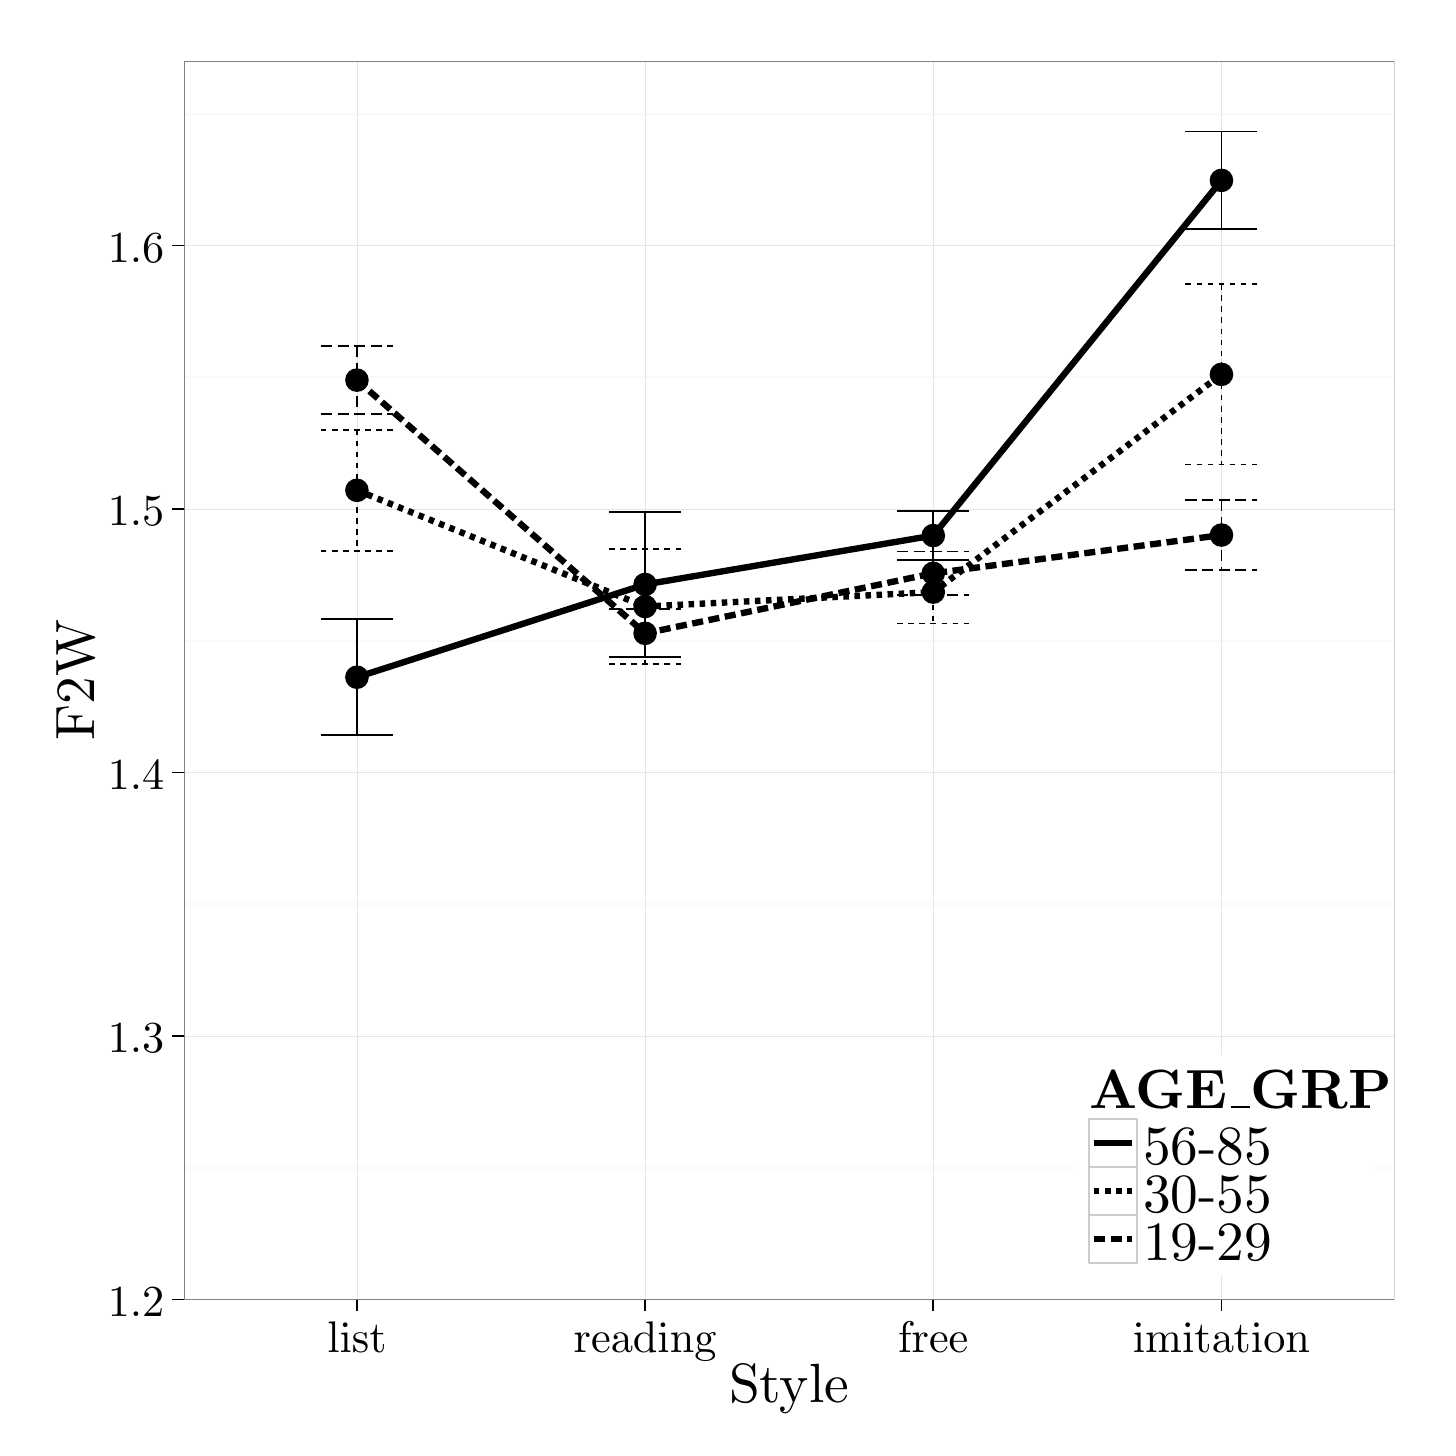
\begin{tikzpicture}[x=1pt,y=1pt]
\definecolor{fillColor}{RGB}{255,255,255}
\path[use as bounding box,fill=fillColor,fill opacity=0.00] (0,0) rectangle (505.89,505.89);
\begin{scope}
\path[clip] (  0.00,  0.00) rectangle (505.89,505.89);
\definecolor{drawColor}{RGB}{255,255,255}
\definecolor{fillColor}{RGB}{255,255,255}

\path[draw=drawColor,line width= 0.6pt,line join=round,line cap=round,fill=fillColor] (  0.00, -0.00) rectangle (505.89,505.89);
\end{scope}
\begin{scope}
\path[clip] ( 56.50, 46.31) rectangle (493.85,493.84);
\definecolor{fillColor}{RGB}{255,255,255}

\path[fill=fillColor] ( 56.50, 46.31) rectangle (493.85,493.84);
\definecolor{drawColor}{gray}{0.98}

\path[draw=drawColor,line width= 0.6pt,line join=round] ( 56.50, 93.92) --
	(493.85, 93.92);

\path[draw=drawColor,line width= 0.6pt,line join=round] ( 56.50,189.14) --
	(493.85,189.14);

\path[draw=drawColor,line width= 0.6pt,line join=round] ( 56.50,284.36) --
	(493.85,284.36);

\path[draw=drawColor,line width= 0.6pt,line join=round] ( 56.50,379.58) --
	(493.85,379.58);

\path[draw=drawColor,line width= 0.6pt,line join=round] ( 56.50,474.80) --
	(493.85,474.80);
\definecolor{drawColor}{gray}{0.90}

\path[draw=drawColor,line width= 0.2pt,line join=round] ( 56.50, 46.31) --
	(493.85, 46.31);

\path[draw=drawColor,line width= 0.2pt,line join=round] ( 56.50,141.53) --
	(493.85,141.53);

\path[draw=drawColor,line width= 0.2pt,line join=round] ( 56.50,236.75) --
	(493.85,236.75);

\path[draw=drawColor,line width= 0.2pt,line join=round] ( 56.50,331.97) --
	(493.85,331.97);

\path[draw=drawColor,line width= 0.2pt,line join=round] ( 56.50,427.19) --
	(493.85,427.19);

\path[draw=drawColor,line width= 0.2pt,line join=round] (118.98, 46.31) --
	(118.98,493.84);

\path[draw=drawColor,line width= 0.2pt,line join=round] (223.11, 46.31) --
	(223.11,493.84);

\path[draw=drawColor,line width= 0.2pt,line join=round] (327.24, 46.31) --
	(327.24,493.84);

\path[draw=drawColor,line width= 0.2pt,line join=round] (431.37, 46.31) --
	(431.37,493.84);
\definecolor{fillColor}{RGB}{0,0,0}

\path[fill=fillColor] (118.98,271.17) circle (  4.27);

\path[fill=fillColor] (118.98,338.71) circle (  4.27);

\path[fill=fillColor] (118.98,378.53) circle (  4.27);

\path[fill=fillColor] (223.11,304.69) circle (  4.27);

\path[fill=fillColor] (223.11,296.72) circle (  4.27);

\path[fill=fillColor] (223.11,287.03) circle (  4.27);

\path[fill=fillColor] (327.24,322.37) circle (  4.27);

\path[fill=fillColor] (327.24,301.93) circle (  4.27);

\path[fill=fillColor] (327.24,308.71) circle (  4.27);

\path[fill=fillColor] (431.37,450.70) circle (  4.27);

\path[fill=fillColor] (431.37,380.60) circle (  4.27);

\path[fill=fillColor] (431.37,322.54) circle (  4.27);
\definecolor{drawColor}{RGB}{0,0,0}

\path[draw=drawColor,line width= 2.3pt,line join=round] (118.98,271.17) --
	(223.11,304.69) --
	(327.24,322.37) --
	(431.37,450.70);

\path[draw=drawColor,line width= 2.3pt,dash pattern=on 2pt off 2pt ,line join=round] (118.98,338.71) --
	(223.11,296.72) --
	(327.24,301.93) --
	(431.37,380.60);

\path[draw=drawColor,line width= 2.3pt,dash pattern=on 4pt off 2pt ,line join=round] (118.98,378.53) --
	(223.11,287.03) --
	(327.24,308.71) --
	(431.37,322.54);

\path[draw=drawColor,line width= 0.6pt,line join=round] (105.96,292.13) --
	(132.00,292.13);

\path[draw=drawColor,line width= 0.6pt,line join=round] (118.98,292.13) --
	(118.98,250.21);

\path[draw=drawColor,line width= 0.6pt,line join=round] (105.96,250.21) --
	(132.00,250.21);

\path[draw=drawColor,line width= 0.6pt,line join=round] (210.09,330.98) --
	(236.13,330.98);

\path[draw=drawColor,line width= 0.6pt,line join=round] (223.11,330.98) --
	(223.11,278.40);

\path[draw=drawColor,line width= 0.6pt,line join=round] (210.09,278.40) --
	(236.13,278.40);

\path[draw=drawColor,line width= 0.6pt,line join=round] (314.22,331.15) --
	(340.25,331.15);

\path[draw=drawColor,line width= 0.6pt,line join=round] (327.24,331.15) --
	(327.24,313.60);

\path[draw=drawColor,line width= 0.6pt,line join=round] (314.22,313.60) --
	(340.25,313.60);

\path[draw=drawColor,line width= 0.6pt,line join=round] (418.35,468.38) --
	(444.38,468.38);

\path[draw=drawColor,line width= 0.6pt,line join=round] (431.37,468.38) --
	(431.37,433.02);

\path[draw=drawColor,line width= 0.6pt,line join=round] (418.35,433.02) --
	(444.38,433.02);

\path[draw=drawColor,line width= 0.6pt,dash pattern=on 2pt off 2pt ,line join=round] (105.96,360.61) --
	(132.00,360.61);

\path[draw=drawColor,line width= 0.6pt,dash pattern=on 2pt off 2pt ,line join=round] (118.98,360.61) --
	(118.98,316.82);

\path[draw=drawColor,line width= 0.6pt,dash pattern=on 2pt off 2pt ,line join=round] (105.96,316.82) --
	(132.00,316.82);

\path[draw=drawColor,line width= 0.6pt,dash pattern=on 2pt off 2pt ,line join=round] (210.09,317.56) --
	(236.13,317.56);

\path[draw=drawColor,line width= 0.6pt,dash pattern=on 2pt off 2pt ,line join=round] (223.11,317.56) --
	(223.11,275.88);

\path[draw=drawColor,line width= 0.6pt,dash pattern=on 2pt off 2pt ,line join=round] (210.09,275.88) --
	(236.13,275.88);

\path[draw=drawColor,line width= 0.6pt,dash pattern=on 2pt off 2pt ,line join=round] (314.22,313.32) --
	(340.25,313.32);

\path[draw=drawColor,line width= 0.6pt,dash pattern=on 2pt off 2pt ,line join=round] (327.24,313.32) --
	(327.24,290.53);

\path[draw=drawColor,line width= 0.6pt,dash pattern=on 2pt off 2pt ,line join=round] (314.22,290.53) --
	(340.25,290.53);

\path[draw=drawColor,line width= 0.6pt,dash pattern=on 2pt off 2pt ,line join=round] (418.35,413.17) --
	(444.38,413.17);

\path[draw=drawColor,line width= 0.6pt,dash pattern=on 2pt off 2pt ,line join=round] (431.37,413.17) --
	(431.37,348.03);

\path[draw=drawColor,line width= 0.6pt,dash pattern=on 2pt off 2pt ,line join=round] (418.35,348.03) --
	(444.38,348.03);

\path[draw=drawColor,line width= 0.6pt,dash pattern=on 4pt off 2pt ,line join=round] (105.96,390.80) --
	(132.00,390.80);

\path[draw=drawColor,line width= 0.6pt,dash pattern=on 4pt off 2pt ,line join=round] (118.98,390.80) --
	(118.98,366.26);

\path[draw=drawColor,line width= 0.6pt,dash pattern=on 4pt off 2pt ,line join=round] (105.96,366.26) --
	(132.00,366.26);

\path[draw=drawColor,line width= 0.6pt,dash pattern=on 4pt off 2pt ,line join=round] (210.09,295.75) --
	(236.13,295.75);

\path[draw=drawColor,line width= 0.6pt,dash pattern=on 4pt off 2pt ,line join=round] (223.11,295.75) --
	(223.11,278.31);

\path[draw=drawColor,line width= 0.6pt,dash pattern=on 4pt off 2pt ,line join=round] (210.09,278.31) --
	(236.13,278.31);

\path[draw=drawColor,line width= 0.6pt,dash pattern=on 4pt off 2pt ,line join=round] (314.22,316.57) --
	(340.25,316.57);

\path[draw=drawColor,line width= 0.6pt,dash pattern=on 4pt off 2pt ,line join=round] (327.24,316.57) --
	(327.24,300.85);

\path[draw=drawColor,line width= 0.6pt,dash pattern=on 4pt off 2pt ,line join=round] (314.22,300.85) --
	(340.25,300.85);

\path[draw=drawColor,line width= 0.6pt,dash pattern=on 4pt off 2pt ,line join=round] (418.35,335.18) --
	(444.38,335.18);

\path[draw=drawColor,line width= 0.6pt,dash pattern=on 4pt off 2pt ,line join=round] (431.37,335.18) --
	(431.37,309.90);

\path[draw=drawColor,line width= 0.6pt,dash pattern=on 4pt off 2pt ,line join=round] (418.35,309.90) --
	(444.38,309.90);
\definecolor{drawColor}{gray}{0.50}

\path[draw=drawColor,line width= 0.6pt,line join=round,line cap=round] ( 56.50, 46.31) rectangle (493.85,493.84);
\end{scope}
\begin{scope}
\path[clip] (  0.00,  0.00) rectangle (505.89,505.89);
\definecolor{drawColor}{RGB}{0,0,0}

\node[text=drawColor,anchor=base east,inner sep=0pt, outer sep=0pt, scale=  1.60] at ( 49.39, 40.27) {1.2};

\node[text=drawColor,anchor=base east,inner sep=0pt, outer sep=0pt, scale=  1.60] at ( 49.39,135.50) {1.3};

\node[text=drawColor,anchor=base east,inner sep=0pt, outer sep=0pt, scale=  1.60] at ( 49.39,230.72) {1.4};

\node[text=drawColor,anchor=base east,inner sep=0pt, outer sep=0pt, scale=  1.60] at ( 49.39,325.94) {1.5};

\node[text=drawColor,anchor=base east,inner sep=0pt, outer sep=0pt, scale=  1.60] at ( 49.39,421.16) {1.6};
\end{scope}
\begin{scope}
\path[clip] (  0.00,  0.00) rectangle (505.89,505.89);
\definecolor{drawColor}{RGB}{0,0,0}

\path[draw=drawColor,line width= 0.6pt,line join=round] ( 52.24, 46.31) --
	( 56.50, 46.31);

\path[draw=drawColor,line width= 0.6pt,line join=round] ( 52.24,141.53) --
	( 56.50,141.53);

\path[draw=drawColor,line width= 0.6pt,line join=round] ( 52.24,236.75) --
	( 56.50,236.75);

\path[draw=drawColor,line width= 0.6pt,line join=round] ( 52.24,331.97) --
	( 56.50,331.97);

\path[draw=drawColor,line width= 0.6pt,line join=round] ( 52.24,427.19) --
	( 56.50,427.19);
\end{scope}
\begin{scope}
\path[clip] (  0.00,  0.00) rectangle (505.89,505.89);
\definecolor{drawColor}{RGB}{0,0,0}

\path[draw=drawColor,line width= 0.6pt,line join=round] (118.98, 42.04) --
	(118.98, 46.31);

\path[draw=drawColor,line width= 0.6pt,line join=round] (223.11, 42.04) --
	(223.11, 46.31);

\path[draw=drawColor,line width= 0.6pt,line join=round] (327.24, 42.04) --
	(327.24, 46.31);

\path[draw=drawColor,line width= 0.6pt,line join=round] (431.37, 42.04) --
	(431.37, 46.31);
\end{scope}
\begin{scope}
\path[clip] (  0.00,  0.00) rectangle (505.89,505.89);
\definecolor{drawColor}{RGB}{0,0,0}

\node[text=drawColor,anchor=base,inner sep=0pt, outer sep=0pt, scale=  1.60] at (118.98, 27.13) {list};

\node[text=drawColor,anchor=base,inner sep=0pt, outer sep=0pt, scale=  1.60] at (223.11, 27.13) {reading};

\node[text=drawColor,anchor=base,inner sep=0pt, outer sep=0pt, scale=  1.60] at (327.24, 27.13) {free};

\node[text=drawColor,anchor=base,inner sep=0pt, outer sep=0pt, scale=  1.60] at (431.37, 27.13) {imitation};
\end{scope}
\begin{scope}
\path[clip] (  0.00,  0.00) rectangle (505.89,505.89);
\definecolor{drawColor}{RGB}{0,0,0}

\node[text=drawColor,anchor=base,inner sep=0pt, outer sep=0pt, scale=  2.00] at (275.17,  9.03) {Style};
\end{scope}
\begin{scope}
\path[clip] (  0.00,  0.00) rectangle (505.89,505.89);
\definecolor{drawColor}{RGB}{0,0,0}

\node[text=drawColor,rotate= 90.00,anchor=base,inner sep=0pt, outer sep=0pt, scale=  2.00] at ( 24.12,270.08) {F2W};
\end{scope}
\begin{scope}
\path[clip] (  0.00,  0.00) rectangle (505.89,505.89);
\definecolor{fillColor}{RGB}{255,255,255}

\path[fill=fillColor] (379.28, 55.18) rectangle (484.98,134.50);
\end{scope}
\begin{scope}
\path[clip] (  0.00,  0.00) rectangle (505.89,505.89);
\definecolor{drawColor}{RGB}{0,0,0}

\node[text=drawColor,anchor=base west,inner sep=0pt, outer sep=0pt, scale=  2.00] at (383.55,115.48) {\bfseries AGE{\_{}}GRP};
\end{scope}
\begin{scope}
\path[clip] (  0.00,  0.00) rectangle (505.89,505.89);
\definecolor{drawColor}{gray}{0.80}
\definecolor{fillColor}{RGB}{255,255,255}

\path[draw=drawColor,line width= 0.6pt,line join=round,line cap=round,fill=fillColor] (383.55, 94.13) rectangle (400.89,111.48);
\end{scope}
\begin{scope}
\path[clip] (  0.00,  0.00) rectangle (505.89,505.89);
\definecolor{drawColor}{RGB}{0,0,0}

\path[draw=drawColor,line width= 2.3pt,line join=round] (385.28,102.81) -- (399.16,102.81);
\end{scope}
\begin{scope}
\path[clip] (  0.00,  0.00) rectangle (505.89,505.89);
\definecolor{drawColor}{RGB}{0,0,0}

\path[draw=drawColor,line width= 0.6pt,line join=round] (385.28,102.81) -- (399.16,102.81);
\end{scope}
\begin{scope}
\path[clip] (  0.00,  0.00) rectangle (505.89,505.89);
\definecolor{drawColor}{gray}{0.80}
\definecolor{fillColor}{RGB}{255,255,255}

\path[draw=drawColor,line width= 0.6pt,line join=round,line cap=round,fill=fillColor] (383.55, 76.79) rectangle (400.89, 94.13);
\end{scope}
\begin{scope}
\path[clip] (  0.00,  0.00) rectangle (505.89,505.89);
\definecolor{drawColor}{RGB}{0,0,0}

\path[draw=drawColor,line width= 2.3pt,dash pattern=on 2pt off 2pt ,line join=round] (385.28, 85.46) -- (399.16, 85.46);
\end{scope}
\begin{scope}
\path[clip] (  0.00,  0.00) rectangle (505.89,505.89);
\definecolor{drawColor}{RGB}{0,0,0}

\path[draw=drawColor,line width= 0.6pt,dash pattern=on 2pt off 2pt ,line join=round] (385.28, 85.46) -- (399.16, 85.46);
\end{scope}
\begin{scope}
\path[clip] (  0.00,  0.00) rectangle (505.89,505.89);
\definecolor{drawColor}{gray}{0.80}
\definecolor{fillColor}{RGB}{255,255,255}

\path[draw=drawColor,line width= 0.6pt,line join=round,line cap=round,fill=fillColor] (383.55, 59.44) rectangle (400.89, 76.79);
\end{scope}
\begin{scope}
\path[clip] (  0.00,  0.00) rectangle (505.89,505.89);
\definecolor{drawColor}{RGB}{0,0,0}

\path[draw=drawColor,line width= 2.3pt,dash pattern=on 4pt off 2pt ,line join=round] (385.28, 68.12) -- (399.16, 68.12);
\end{scope}
\begin{scope}
\path[clip] (  0.00,  0.00) rectangle (505.89,505.89);
\definecolor{drawColor}{RGB}{0,0,0}

\path[draw=drawColor,line width= 0.6pt,dash pattern=on 4pt off 2pt ,line join=round] (385.28, 68.12) -- (399.16, 68.12);
\end{scope}
\begin{scope}
\path[clip] (  0.00,  0.00) rectangle (505.89,505.89);
\definecolor{drawColor}{RGB}{0,0,0}

\node[text=drawColor,anchor=base west,inner sep=0pt, outer sep=0pt, scale=  2.00] at (403.06, 95.26) {56-85};
\end{scope}
\begin{scope}
\path[clip] (  0.00,  0.00) rectangle (505.89,505.89);
\definecolor{drawColor}{RGB}{0,0,0}

\node[text=drawColor,anchor=base west,inner sep=0pt, outer sep=0pt, scale=  2.00] at (403.06, 77.92) {30-55};
\end{scope}
\begin{scope}
\path[clip] (  0.00,  0.00) rectangle (505.89,505.89);
\definecolor{drawColor}{RGB}{0,0,0}

\node[text=drawColor,anchor=base west,inner sep=0pt, outer sep=0pt, scale=  2.00] at (403.06, 60.57) {19-29};
\end{scope}
\end{tikzpicture}
} 
		\caption{working class}
		\label{fig.line.f2.nurse.wc}
	\end{subfigure}
	\caption{\textsc{nurse} (F2) by style, age, and social class}
\end{figure}

Since the mixed linear effects regression also found a three-way interaction of style, age, and social class of participant, we will end this section with an analysis of two figures that illustrate the interaction of style and age for middle-class (Figure \ref{fig.line.f2.nurse.mc}) and working-class subjects (Figure \ref{fig.line.f2.nurse.wc}), respectively.
Class seems to play the least important role for the oldest interviewees in the sample.
Middle-class speakers in this age group have an almost flat line for the first three registers: there \emph{is} a slight but significant drop from `reading' to `free', but word list realisations are neither significantly different from those in the reading passage, nor from the variants that are found in spontaneous speech.
Accent imitation\is{accent performance} is significantly (and drastically) fronter than the other three registers.
The solid line in Figure \ref{fig.line.f2.nurse.wc} suggests a more steady increase of F2, but `list' is not significantly different from `reading', which in turn is not significantly different from `free' (`list' and `free', however, are) --- statistically speaking, this line can be thought of as flat for the first three styles, just as in Figure \ref{fig.line.f2.nurse.mc}.

The dotted line (middle-aged subjects) in Figure \ref{fig.line.f2.nurse.mc} is very similar to the one found for the entire dataset in Figure \ref{fig.line.f2.nurse.tot}.
Word list and reading passage are not significantly different, F2 drops significantly in free speech, and rises significantly again in accent perform\is{accent performance}ance.
Working-class speakers in this age group, on the other hand, have statistically identical \textsc{nurse} variants in free speech and while reading a text.
\textsc{nurse} is again fronter when people imitate a strong Scouse accent, but the vowel is actually just as advanced in the word list, the register which was supposed to elicit more standard pronunciations.

For the youngest speakers in the sample the class distinction is most interesting.
Middle-class speakers exhibit a statistically completely level line for the first three styles, followed by the same rise in F2 for `imitation\is{accent performance}' as in the old and the middle-aged subjects.
Working-class speakers, on the other hand, do not significantly distinguish free speech from accent perform\is{accent performance}ance.
They do, however, have significantly more retracted variants when reading out a text (as compared to spontaneous pronunciations in connected speech).
Furthermore, when reading out a word list young working-class speakers actually have more advanced (more Scouse) \textsc{nurse} realisations than in any other register.
The shifting found in Figure \ref{fig.line.f2.nurse.tot} for the youngest speakers thus seems to be a true combination of these two diametrically opposed patterns: The significant fronting of \textsc{nurse} during accent perform\is{accent performance}ance is due to middle-class speakers, whereas their working-class counterparts contribute the fronting in the most formal word list style (and also drive the rise in F2 from `reading' to `free').

\subsection{Synthesis and Pillai scores (\textsc{nurse})}
\label{sec.prod.res.vow.nurse.pil}

\subsubsection{Overview}
Up until now, the analysis has exclusively focused on the realisation of \textsc{nurse}, despite the fact that we are dealing with a vowel \emph{merger} here.
Since (near-standard) \textsc{square} is generally considered to be the target of this merger in Liverpool, said focus on \textsc{nurse} does not seem unjustified, since it is mostly in the latter one that variation is to be expected.
Nevertheless, the other member of the pair should not totally be neglected.
After all, it could well be that both \textsc{nurse} and \textsc{square} are, for example, fronted by a particular group of speakers.
This \emph{might} still make them sound more Scouse (because \textsc{nurse} would be moving further away from the standard), but not necessarily so because it is primarily the merger of these two vowels that is considered a characteristic feature of the accent.
While constraints of space do not permit a detailed analysis of \textsc{square} (such as the one provided for \textsc{nurse} in Sections \ref{sec.prod.res.vow.nurse.f1} and \ref{sec.prod.res.vow.nurse.f2}), the remainder of this chapter will at least have a brief look at the realisational spaces of both \textsc{nurse} \emph{and} \textsc{square} in the different age groups, and it will also consider \isi{Pillai} scores calculated on the basis of these distributions.

\begin{table}[h!]
	\centering
	\caption{\textsc{nurse}-\textsc{square}: Pillai scores by age and style (groups)}
	\label{tab.pillai.nurse.agestyle}
	\begin{tabular}{lrrrrrr}
		\hline
		& \multicolumn{2}{c}{old} & \multicolumn{2}{c}{middle} & \multicolumn{2}{c}{young}\\
		style & \isi{Pillai} & p-value & \isi{Pillai} & p-value & \isi{Pillai} & p-value\\
		\hline
		word list & 0.021 & 0.436 & 0.015 & 0.333 & 0.025 & 0.150\\
		reading & 0.026 & 0.315 & 0.017 & 0.208 & 0.034 & 0.051\\
		free & 0.073 & < 0.001 & 0.050 & < 0.001 & 0.025 & 0.007\\
		imitation\is{accent performance} & 0.016 & 0.533 & 0.007 & 0.727 & 0.014 & 0.398\\
		total & 0.046 & < 0.001 & 0.031 & < 0.001 & 0.013 & 0.004\\
		\hline
	\end{tabular}
\end{table}

Table \ref{tab.pillai.nurse.agestyle} summarises the results of a number of \textsc{manova}s, which were carried out in each age group and in each speaking style separately.
The last line in this table (which reports the tests performed on all \textsc{nurse} and \textsc{square} observations within the respective age group, pooled across style) tells us that \textsc{nurse} and \textsc{square} distributions are (highly) significantly different in all three age groups investigated --- all p-values are well below the 5\% threshold.
However, these values must be interpreted in connection with the \isi{Pillai} scores that go with them, and which are just as homogeneous as the p-values: all of them are close to 0 (remember that \isi{Pillai} scores can have values between 0 and 1), which indicates almost perfect overlap between the two (merged) vowel distributions.
It is therefore more than likely that the low p-values are simply due to the large amount of data that are available when the observations are pooled across speaking styles, because in a sufficiently large dataset \emph{any} difference will turn out to be statistically significant.
We can therefore say that all three generations of speakers have completely merged \textsc{nurse} and \textsc{square} distributions.

Judging from Table \ref{tab.pillai.nurse.agestyle}, style does not seem to make much of a difference either.
It is true that some \isi{Pillai} scores calculated for a particular register are almost twice (or, in the case of the youngest speakers, even thrice) as large as the total score in the last line, but even so all \isi{Pillai} scores are (considerably) below 0.1, meaning they hardly differ from the total scores in absolute terms.
This time, p-values support the idea that distributions are almost perfectly merged: With the exception of the ones pertaining to spontaneous speech (which accounts for the lion share of the data in each age group), no p-value is below the 5\% threshold.
All age groups seem to have merged vowel distributions in all four speaking styles for which data were collected.

\subsubsection{Old speakers}

\begin{figure}[h!]
	\centering
	\begin{subfigure}{.49\textwidth}
		\centering
			\definecolor{shadecolor}{rgb}{0.969, 0.969, 0.969}
			\resizebox{\linewidth}{!}{% Created by tikzDevice version 0.8.1 on 2016-02-09 02:15:18
% !TEX encoding = UTF-8 Unicode
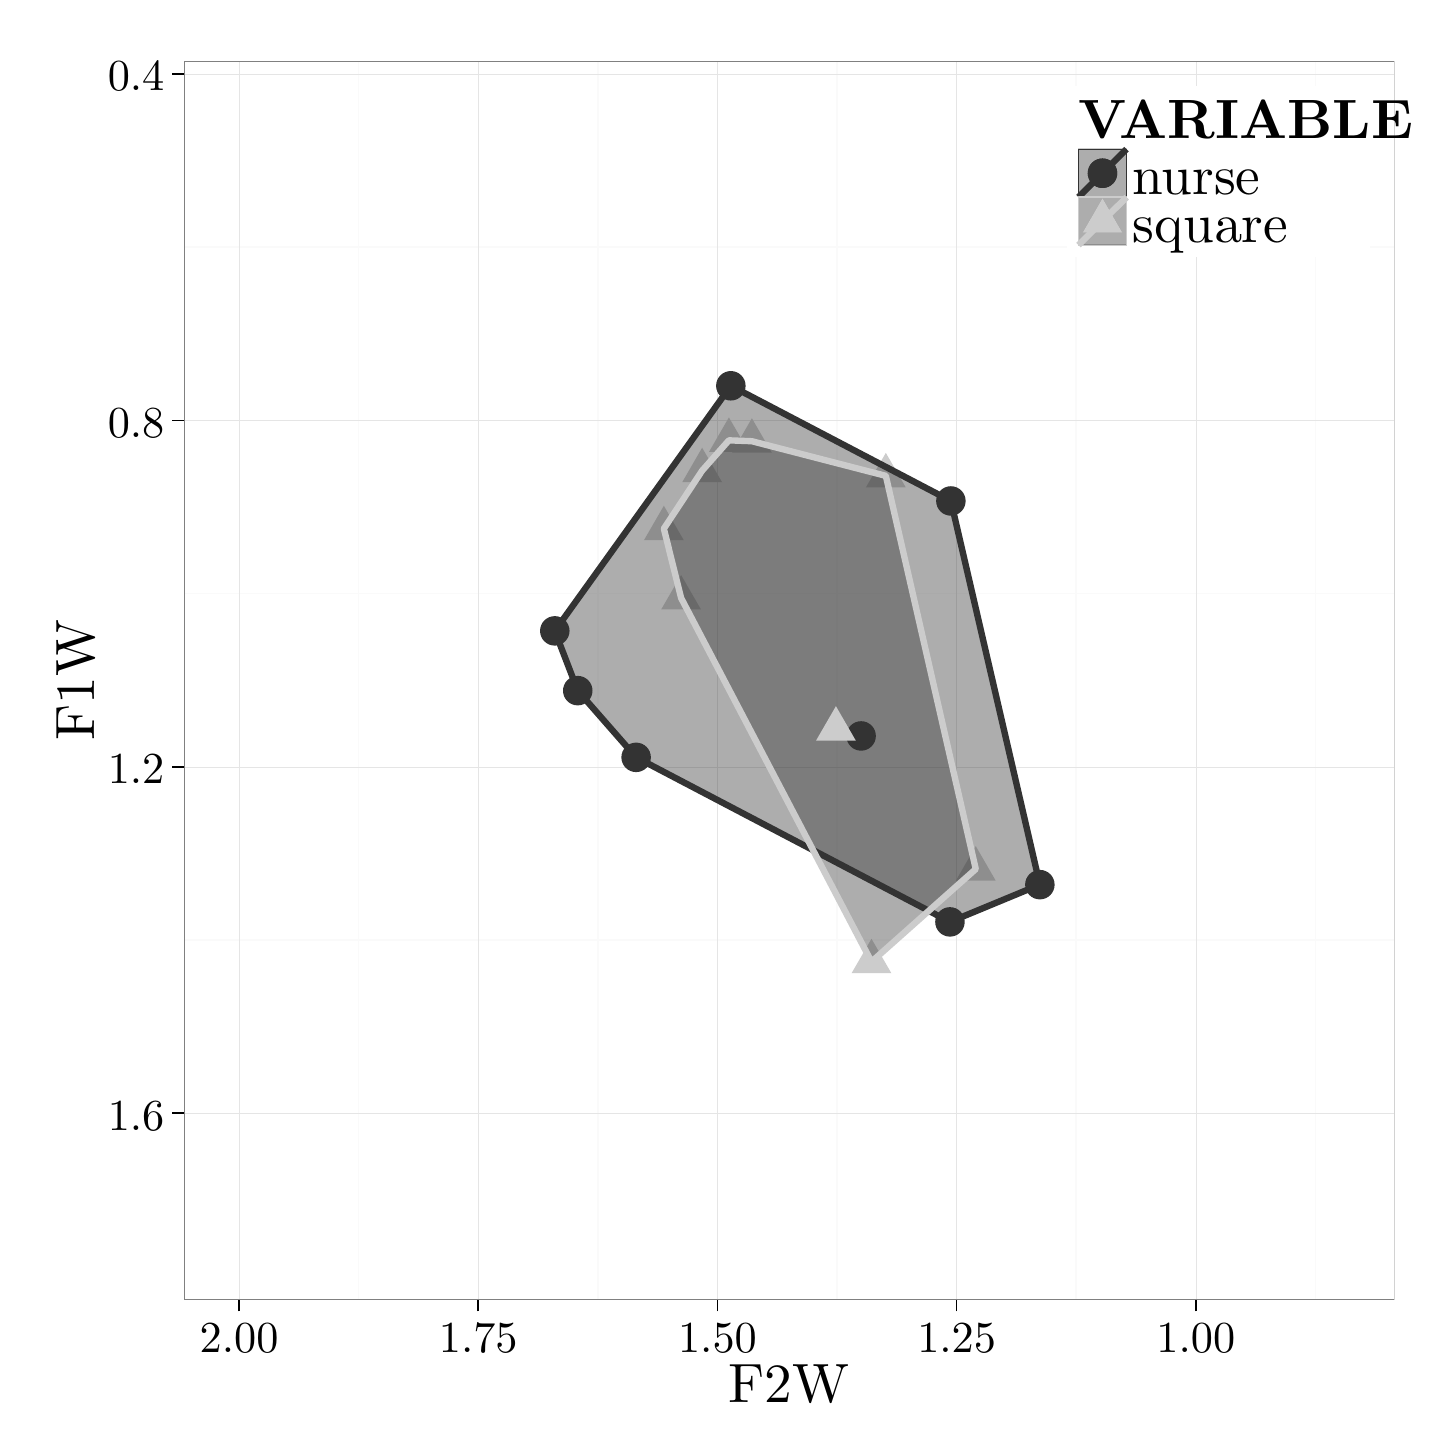
\begin{tikzpicture}[x=1pt,y=1pt]
\definecolor{fillColor}{RGB}{255,255,255}
\path[use as bounding box,fill=fillColor,fill opacity=0.00] (0,0) rectangle (505.89,505.89);
\begin{scope}
\path[clip] (  0.00,  0.00) rectangle (505.89,505.89);
\definecolor{drawColor}{RGB}{255,255,255}
\definecolor{fillColor}{RGB}{255,255,255}

\path[draw=drawColor,line width= 0.6pt,line join=round,line cap=round,fill=fillColor] (  0.00, -0.00) rectangle (505.89,505.89);
\end{scope}
\begin{scope}
\path[clip] ( 56.50, 46.31) rectangle (493.85,493.84);
\definecolor{fillColor}{RGB}{255,255,255}

\path[fill=fillColor] ( 56.50, 46.31) rectangle (493.85,493.84);
\definecolor{drawColor}{gray}{0.98}

\path[draw=drawColor,line width= 0.6pt,line join=round] ( 56.50,426.56) --
	(493.85,426.56);

\path[draw=drawColor,line width= 0.6pt,line join=round] ( 56.50,301.37) --
	(493.85,301.37);

\path[draw=drawColor,line width= 0.6pt,line join=round] ( 56.50,176.19) --
	(493.85,176.19);

\path[draw=drawColor,line width= 0.6pt,line join=round] (465.32, 46.31) --
	(465.32,493.84);

\path[draw=drawColor,line width= 0.6pt,line join=round] (378.89, 46.31) --
	(378.89,493.84);

\path[draw=drawColor,line width= 0.6pt,line join=round] (292.46, 46.31) --
	(292.46,493.84);

\path[draw=drawColor,line width= 0.6pt,line join=round] (206.03, 46.31) --
	(206.03,493.84);

\path[draw=drawColor,line width= 0.6pt,line join=round] (119.60, 46.31) --
	(119.60,493.84);
\definecolor{drawColor}{gray}{0.90}

\path[draw=drawColor,line width= 0.2pt,line join=round] ( 56.50,489.15) --
	(493.85,489.15);

\path[draw=drawColor,line width= 0.2pt,line join=round] ( 56.50,363.97) --
	(493.85,363.97);

\path[draw=drawColor,line width= 0.2pt,line join=round] ( 56.50,238.78) --
	(493.85,238.78);

\path[draw=drawColor,line width= 0.2pt,line join=round] ( 56.50,113.59) --
	(493.85,113.59);

\path[draw=drawColor,line width= 0.2pt,line join=round] (422.11, 46.31) --
	(422.11,493.84);

\path[draw=drawColor,line width= 0.2pt,line join=round] (335.68, 46.31) --
	(335.68,493.84);

\path[draw=drawColor,line width= 0.2pt,line join=round] (249.24, 46.31) --
	(249.24,493.84);

\path[draw=drawColor,line width= 0.2pt,line join=round] (162.81, 46.31) --
	(162.81,493.84);

\path[draw=drawColor,line width= 0.2pt,line join=round] ( 76.38, 46.31) --
	( 76.38,493.84);
\definecolor{fillColor}{gray}{0.20}

\path[fill=fillColor] (190.47,287.92) circle (  5.33);

\path[fill=fillColor] (254.09,376.48) circle (  5.33);

\path[fill=fillColor] (333.60,334.86) circle (  5.33);

\path[fill=fillColor] (365.75,196.22) circle (  5.33);

\path[fill=fillColor] (333.26,182.76) circle (  5.33);

\path[fill=fillColor] (219.86,242.22) circle (  5.33);

\path[fill=fillColor] (198.77,266.32) circle (  5.33);
\definecolor{fillColor}{gray}{0.80}

\path[fill=fillColor] (236.11,308.10) --
	(243.29,295.66) --
	(228.92,295.66) --
	cycle;

\path[fill=fillColor] (229.88,333.14) --
	(237.07,320.70) --
	(222.70,320.70) --
	cycle;

\path[fill=fillColor] (243.71,354.11) --
	(250.90,341.67) --
	(236.53,341.67) --
	cycle;

\path[fill=fillColor] (253.39,365.06) --
	(260.58,352.62) --
	(246.21,352.62) --
	cycle;

\path[fill=fillColor] (261.69,364.75) --
	(268.88,352.31) --
	(254.51,352.31) --
	cycle;

\path[fill=fillColor] (310.09,352.23) --
	(317.28,339.79) --
	(302.91,339.79) --
	cycle;

\path[fill=fillColor] (342.59,210.15) --
	(349.78,197.70) --
	(335.41,197.70) --
	cycle;

\path[fill=fillColor] (304.91,176.66) --
	(312.09,164.22) --
	(297.72,164.22) --
	cycle;
\definecolor{drawColor}{gray}{0.20}
\definecolor{fillColor}{RGB}{51,51,51}

\path[draw=drawColor,line width= 2.3pt,line join=round,line cap=round,fill=fillColor,fill opacity=0.40] (190.47,287.92) --
	(254.09,376.48) --
	(333.60,334.86) --
	(365.75,196.22) --
	(333.26,182.76) --
	(219.86,242.22) --
	(198.77,266.32) --
	cycle;
\definecolor{drawColor}{gray}{0.80}

\path[draw=drawColor,line width= 2.3pt,line join=round,line cap=round,fill=fillColor,fill opacity=0.40] (236.11,299.81) --
	(229.88,324.84) --
	(243.71,345.81) --
	(253.39,356.77) --
	(261.69,356.45) --
	(310.09,343.94) --
	(342.59,201.85) --
	(304.91,168.36) --
	cycle;
\definecolor{fillColor}{gray}{0.20}

\path[fill=fillColor] (301.16,249.95) circle (  5.33);
\definecolor{fillColor}{gray}{0.80}

\path[fill=fillColor] (292.06,260.71) --
	(299.24,248.26) --
	(284.87,248.26) --
	cycle;
\definecolor{drawColor}{gray}{0.50}

\path[draw=drawColor,line width= 0.6pt,line join=round,line cap=round] ( 56.50, 46.31) rectangle (493.85,493.84);
\end{scope}
\begin{scope}
\path[clip] (  0.00,  0.00) rectangle (505.89,505.89);
\definecolor{drawColor}{RGB}{0,0,0}

\node[text=drawColor,anchor=base east,inner sep=0pt, outer sep=0pt, scale=  1.60] at ( 49.39,483.12) {0.4};

\node[text=drawColor,anchor=base east,inner sep=0pt, outer sep=0pt, scale=  1.60] at ( 49.39,357.93) {0.8};

\node[text=drawColor,anchor=base east,inner sep=0pt, outer sep=0pt, scale=  1.60] at ( 49.39,232.75) {1.2};

\node[text=drawColor,anchor=base east,inner sep=0pt, outer sep=0pt, scale=  1.60] at ( 49.39,107.56) {1.6};
\end{scope}
\begin{scope}
\path[clip] (  0.00,  0.00) rectangle (505.89,505.89);
\definecolor{drawColor}{RGB}{0,0,0}

\path[draw=drawColor,line width= 0.6pt,line join=round] ( 52.24,489.15) --
	( 56.50,489.15);

\path[draw=drawColor,line width= 0.6pt,line join=round] ( 52.24,363.97) --
	( 56.50,363.97);

\path[draw=drawColor,line width= 0.6pt,line join=round] ( 52.24,238.78) --
	( 56.50,238.78);

\path[draw=drawColor,line width= 0.6pt,line join=round] ( 52.24,113.59) --
	( 56.50,113.59);
\end{scope}
\begin{scope}
\path[clip] (  0.00,  0.00) rectangle (505.89,505.89);
\definecolor{drawColor}{RGB}{0,0,0}

\path[draw=drawColor,line width= 0.6pt,line join=round] (422.11, 42.04) --
	(422.11, 46.31);

\path[draw=drawColor,line width= 0.6pt,line join=round] (335.68, 42.04) --
	(335.68, 46.31);

\path[draw=drawColor,line width= 0.6pt,line join=round] (249.24, 42.04) --
	(249.24, 46.31);

\path[draw=drawColor,line width= 0.6pt,line join=round] (162.81, 42.04) --
	(162.81, 46.31);

\path[draw=drawColor,line width= 0.6pt,line join=round] ( 76.38, 42.04) --
	( 76.38, 46.31);
\end{scope}
\begin{scope}
\path[clip] (  0.00,  0.00) rectangle (505.89,505.89);
\definecolor{drawColor}{RGB}{0,0,0}

\node[text=drawColor,anchor=base,inner sep=0pt, outer sep=0pt, scale=  1.60] at (422.11, 27.13) {1.00};

\node[text=drawColor,anchor=base,inner sep=0pt, outer sep=0pt, scale=  1.60] at (335.68, 27.13) {1.25};

\node[text=drawColor,anchor=base,inner sep=0pt, outer sep=0pt, scale=  1.60] at (249.24, 27.13) {1.50};

\node[text=drawColor,anchor=base,inner sep=0pt, outer sep=0pt, scale=  1.60] at (162.81, 27.13) {1.75};

\node[text=drawColor,anchor=base,inner sep=0pt, outer sep=0pt, scale=  1.60] at ( 76.38, 27.13) {2.00};
\end{scope}
\begin{scope}
\path[clip] (  0.00,  0.00) rectangle (505.89,505.89);
\definecolor{drawColor}{RGB}{0,0,0}

\node[text=drawColor,anchor=base,inner sep=0pt, outer sep=0pt, scale=  2.00] at (275.17,  9.03) {F2W};
\end{scope}
\begin{scope}
\path[clip] (  0.00,  0.00) rectangle (505.89,505.89);
\definecolor{drawColor}{RGB}{0,0,0}

\node[text=drawColor,rotate= 90.00,anchor=base,inner sep=0pt, outer sep=0pt, scale=  2.00] at ( 24.12,270.08) {F1W};
\end{scope}
\begin{scope}
\path[clip] (  0.00,  0.00) rectangle (505.89,505.89);
\definecolor{fillColor}{RGB}{255,255,255}

\path[fill=fillColor] (375.44,423.00) rectangle (484.98,484.98);
\end{scope}
\begin{scope}
\path[clip] (  0.00,  0.00) rectangle (505.89,505.89);
\definecolor{drawColor}{RGB}{0,0,0}

\node[text=drawColor,anchor=base west,inner sep=0pt, outer sep=0pt, scale=  2.00] at (379.71,465.96) {\bfseries VARIABLE};
\end{scope}
\begin{scope}
\path[clip] (  0.00,  0.00) rectangle (505.89,505.89);
\definecolor{drawColor}{gray}{0.80}
\definecolor{fillColor}{RGB}{255,255,255}

\path[draw=drawColor,line width= 0.6pt,line join=round,line cap=round,fill=fillColor] (379.71,444.61) rectangle (397.06,461.96);
\end{scope}
\begin{scope}
\path[clip] (  0.00,  0.00) rectangle (505.89,505.89);
\definecolor{fillColor}{gray}{0.20}

\path[fill=fillColor] (388.38,453.29) circle (  5.33);
\end{scope}
\begin{scope}
\path[clip] (  0.00,  0.00) rectangle (505.89,505.89);
\definecolor{drawColor}{gray}{0.20}
\definecolor{fillColor}{RGB}{51,51,51}

\path[draw=drawColor,line width= 0.4pt,line join=round,line cap=round,fill=fillColor,fill opacity=0.40] (379.71,444.61) rectangle (397.06,461.96);

\path[draw=drawColor,line width= 2.3pt,line join=round] (379.71,444.61) --
	(397.06,461.96);
\end{scope}
\begin{scope}
\path[clip] (  0.00,  0.00) rectangle (505.89,505.89);
\definecolor{fillColor}{gray}{0.20}

\path[fill=fillColor] (388.38,453.29) circle (  5.33);
\end{scope}
\begin{scope}
\path[clip] (  0.00,  0.00) rectangle (505.89,505.89);
\definecolor{drawColor}{gray}{0.80}
\definecolor{fillColor}{RGB}{255,255,255}

\path[draw=drawColor,line width= 0.6pt,line join=round,line cap=round,fill=fillColor] (379.71,427.27) rectangle (397.06,444.61);
\end{scope}
\begin{scope}
\path[clip] (  0.00,  0.00) rectangle (505.89,505.89);
\definecolor{fillColor}{gray}{0.80}

\path[fill=fillColor] (388.38,444.24) --
	(395.57,431.79) --
	(381.20,431.79) --
	cycle;
\end{scope}
\begin{scope}
\path[clip] (  0.00,  0.00) rectangle (505.89,505.89);
\definecolor{drawColor}{gray}{0.80}
\definecolor{fillColor}{RGB}{51,51,51}

\path[draw=drawColor,line width= 0.4pt,line join=round,line cap=round,fill=fillColor,fill opacity=0.40] (379.71,427.27) rectangle (397.06,444.61);

\path[draw=drawColor,line width= 2.3pt,line join=round] (379.71,427.27) --
	(397.06,444.61);
\end{scope}
\begin{scope}
\path[clip] (  0.00,  0.00) rectangle (505.89,505.89);
\definecolor{fillColor}{gray}{0.80}

\path[fill=fillColor] (388.38,444.24) --
	(395.57,431.79) --
	(381.20,431.79) --
	cycle;
\end{scope}
\begin{scope}
\path[clip] (  0.00,  0.00) rectangle (505.89,505.89);
\definecolor{drawColor}{RGB}{0,0,0}

\node[text=drawColor,anchor=base west,inner sep=0pt, outer sep=0pt, scale=  2.00] at (399.22,445.75) {nurse};
\end{scope}
\begin{scope}
\path[clip] (  0.00,  0.00) rectangle (505.89,505.89);
\definecolor{drawColor}{RGB}{0,0,0}

\node[text=drawColor,anchor=base west,inner sep=0pt, outer sep=0pt, scale=  2.00] at (399.22,428.40) {square};
\end{scope}
\end{tikzpicture}
} 
		\caption{word list}
		\label{fig.nurse.space.old.list}
	\end{subfigure}
	\begin{subfigure}{.49\textwidth}
		\centering
			\definecolor{shadecolor}{rgb}{0.969, 0.969, 0.969}
			\resizebox{\linewidth}{!}{% Created by tikzDevice version 0.8.1 on 2016-02-09 02:15:21
% !TEX encoding = UTF-8 Unicode
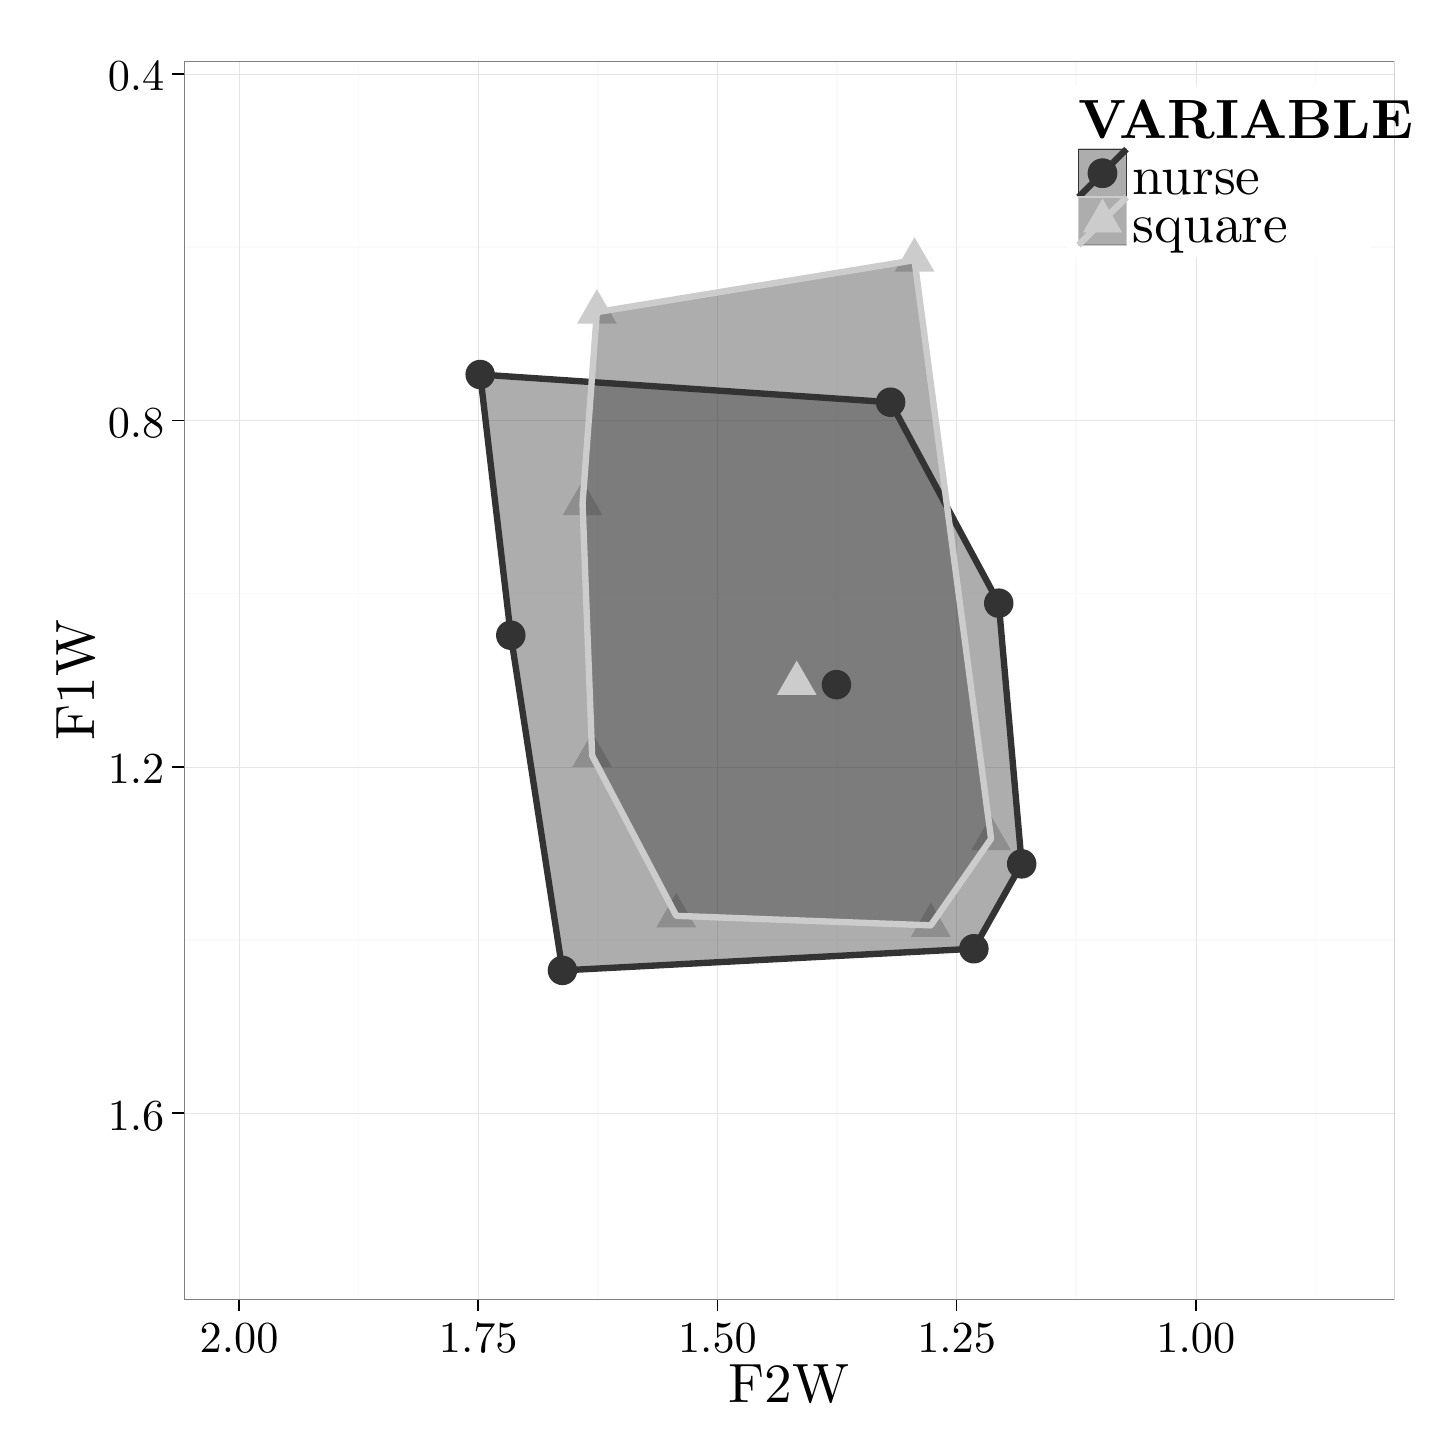
\begin{tikzpicture}[x=1pt,y=1pt]
\definecolor{fillColor}{RGB}{255,255,255}
\path[use as bounding box,fill=fillColor,fill opacity=0.00] (0,0) rectangle (505.89,505.89);
\begin{scope}
\path[clip] (  0.00,  0.00) rectangle (505.89,505.89);
\definecolor{drawColor}{RGB}{255,255,255}
\definecolor{fillColor}{RGB}{255,255,255}

\path[draw=drawColor,line width= 0.6pt,line join=round,line cap=round,fill=fillColor] (  0.00, -0.00) rectangle (505.89,505.89);
\end{scope}
\begin{scope}
\path[clip] ( 56.50, 46.31) rectangle (493.85,493.84);
\definecolor{fillColor}{RGB}{255,255,255}

\path[fill=fillColor] ( 56.50, 46.31) rectangle (493.85,493.84);
\definecolor{drawColor}{gray}{0.98}

\path[draw=drawColor,line width= 0.6pt,line join=round] ( 56.50,426.56) --
	(493.85,426.56);

\path[draw=drawColor,line width= 0.6pt,line join=round] ( 56.50,301.37) --
	(493.85,301.37);

\path[draw=drawColor,line width= 0.6pt,line join=round] ( 56.50,176.19) --
	(493.85,176.19);

\path[draw=drawColor,line width= 0.6pt,line join=round] (465.32, 46.31) --
	(465.32,493.84);

\path[draw=drawColor,line width= 0.6pt,line join=round] (378.89, 46.31) --
	(378.89,493.84);

\path[draw=drawColor,line width= 0.6pt,line join=round] (292.46, 46.31) --
	(292.46,493.84);

\path[draw=drawColor,line width= 0.6pt,line join=round] (206.03, 46.31) --
	(206.03,493.84);

\path[draw=drawColor,line width= 0.6pt,line join=round] (119.60, 46.31) --
	(119.60,493.84);
\definecolor{drawColor}{gray}{0.90}

\path[draw=drawColor,line width= 0.2pt,line join=round] ( 56.50,489.15) --
	(493.85,489.15);

\path[draw=drawColor,line width= 0.2pt,line join=round] ( 56.50,363.97) --
	(493.85,363.97);

\path[draw=drawColor,line width= 0.2pt,line join=round] ( 56.50,238.78) --
	(493.85,238.78);

\path[draw=drawColor,line width= 0.2pt,line join=round] ( 56.50,113.59) --
	(493.85,113.59);

\path[draw=drawColor,line width= 0.2pt,line join=round] (422.11, 46.31) --
	(422.11,493.84);

\path[draw=drawColor,line width= 0.2pt,line join=round] (335.68, 46.31) --
	(335.68,493.84);

\path[draw=drawColor,line width= 0.2pt,line join=round] (249.24, 46.31) --
	(249.24,493.84);

\path[draw=drawColor,line width= 0.2pt,line join=round] (162.81, 46.31) --
	(162.81,493.84);

\path[draw=drawColor,line width= 0.2pt,line join=round] ( 76.38, 46.31) --
	( 76.38,493.84);
\definecolor{fillColor}{gray}{0.20}

\path[fill=fillColor] (174.57,286.35) circle (  5.33);

\path[fill=fillColor] (163.51,380.55) circle (  5.33);

\path[fill=fillColor] (311.82,370.54) circle (  5.33);

\path[fill=fillColor] (350.89,297.93) circle (  5.33);

\path[fill=fillColor] (359.19,203.73) circle (  5.33);

\path[fill=fillColor] (341.90,173.06) circle (  5.33);

\path[fill=fillColor] (193.24,165.23) circle (  5.33);
\definecolor{fillColor}{gray}{0.80}

\path[fill=fillColor] (200.50,342.22) --
	(207.68,329.77) --
	(193.31,329.77) --
	cycle;

\path[fill=fillColor] (205.68,411.38) --
	(212.87,398.94) --
	(198.50,398.94) --
	cycle;

\path[fill=fillColor] (320.46,430.16) --
	(327.65,417.72) --
	(313.28,417.72) --
	cycle;

\path[fill=fillColor] (348.12,221.10) --
	(355.31,208.66) --
	(340.94,208.66) --
	cycle;

\path[fill=fillColor] (326.34,189.80) --
	(333.53,177.36) --
	(319.16,177.36) --
	cycle;

\path[fill=fillColor] (234.38,193.25) --
	(241.56,180.80) --
	(227.19,180.80) --
	cycle;

\path[fill=fillColor] (203.96,251.14) --
	(211.14,238.70) --
	(196.77,238.70) --
	cycle;
\definecolor{drawColor}{gray}{0.20}
\definecolor{fillColor}{RGB}{51,51,51}

\path[draw=drawColor,line width= 2.3pt,line join=round,line cap=round,fill=fillColor,fill opacity=0.40] (174.57,286.35) --
	(163.51,380.55) --
	(311.82,370.54) --
	(350.89,297.93) --
	(359.19,203.73) --
	(341.90,173.06) --
	(193.24,165.23) --
	cycle;
\definecolor{drawColor}{gray}{0.80}

\path[draw=drawColor,line width= 2.3pt,line join=round,line cap=round,fill=fillColor,fill opacity=0.40] (200.50,333.92) --
	(205.68,403.09) --
	(320.46,421.86) --
	(348.12,212.80) --
	(326.34,181.51) --
	(234.38,184.95) --
	(203.96,242.85) --
	cycle;
\definecolor{fillColor}{gray}{0.20}

\path[fill=fillColor] (292.25,268.49) circle (  5.33);
\definecolor{fillColor}{gray}{0.80}

\path[fill=fillColor] (277.90,277.20) --
	(285.08,264.76) --
	(270.71,264.76) --
	cycle;
\definecolor{drawColor}{gray}{0.50}

\path[draw=drawColor,line width= 0.6pt,line join=round,line cap=round] ( 56.50, 46.31) rectangle (493.85,493.84);
\end{scope}
\begin{scope}
\path[clip] (  0.00,  0.00) rectangle (505.89,505.89);
\definecolor{drawColor}{RGB}{0,0,0}

\node[text=drawColor,anchor=base east,inner sep=0pt, outer sep=0pt, scale=  1.60] at ( 49.39,483.12) {0.4};

\node[text=drawColor,anchor=base east,inner sep=0pt, outer sep=0pt, scale=  1.60] at ( 49.39,357.93) {0.8};

\node[text=drawColor,anchor=base east,inner sep=0pt, outer sep=0pt, scale=  1.60] at ( 49.39,232.75) {1.2};

\node[text=drawColor,anchor=base east,inner sep=0pt, outer sep=0pt, scale=  1.60] at ( 49.39,107.56) {1.6};
\end{scope}
\begin{scope}
\path[clip] (  0.00,  0.00) rectangle (505.89,505.89);
\definecolor{drawColor}{RGB}{0,0,0}

\path[draw=drawColor,line width= 0.6pt,line join=round] ( 52.24,489.15) --
	( 56.50,489.15);

\path[draw=drawColor,line width= 0.6pt,line join=round] ( 52.24,363.97) --
	( 56.50,363.97);

\path[draw=drawColor,line width= 0.6pt,line join=round] ( 52.24,238.78) --
	( 56.50,238.78);

\path[draw=drawColor,line width= 0.6pt,line join=round] ( 52.24,113.59) --
	( 56.50,113.59);
\end{scope}
\begin{scope}
\path[clip] (  0.00,  0.00) rectangle (505.89,505.89);
\definecolor{drawColor}{RGB}{0,0,0}

\path[draw=drawColor,line width= 0.6pt,line join=round] (422.11, 42.04) --
	(422.11, 46.31);

\path[draw=drawColor,line width= 0.6pt,line join=round] (335.68, 42.04) --
	(335.68, 46.31);

\path[draw=drawColor,line width= 0.6pt,line join=round] (249.24, 42.04) --
	(249.24, 46.31);

\path[draw=drawColor,line width= 0.6pt,line join=round] (162.81, 42.04) --
	(162.81, 46.31);

\path[draw=drawColor,line width= 0.6pt,line join=round] ( 76.38, 42.04) --
	( 76.38, 46.31);
\end{scope}
\begin{scope}
\path[clip] (  0.00,  0.00) rectangle (505.89,505.89);
\definecolor{drawColor}{RGB}{0,0,0}

\node[text=drawColor,anchor=base,inner sep=0pt, outer sep=0pt, scale=  1.60] at (422.11, 27.13) {1.00};

\node[text=drawColor,anchor=base,inner sep=0pt, outer sep=0pt, scale=  1.60] at (335.68, 27.13) {1.25};

\node[text=drawColor,anchor=base,inner sep=0pt, outer sep=0pt, scale=  1.60] at (249.24, 27.13) {1.50};

\node[text=drawColor,anchor=base,inner sep=0pt, outer sep=0pt, scale=  1.60] at (162.81, 27.13) {1.75};

\node[text=drawColor,anchor=base,inner sep=0pt, outer sep=0pt, scale=  1.60] at ( 76.38, 27.13) {2.00};
\end{scope}
\begin{scope}
\path[clip] (  0.00,  0.00) rectangle (505.89,505.89);
\definecolor{drawColor}{RGB}{0,0,0}

\node[text=drawColor,anchor=base,inner sep=0pt, outer sep=0pt, scale=  2.00] at (275.17,  9.03) {F2W};
\end{scope}
\begin{scope}
\path[clip] (  0.00,  0.00) rectangle (505.89,505.89);
\definecolor{drawColor}{RGB}{0,0,0}

\node[text=drawColor,rotate= 90.00,anchor=base,inner sep=0pt, outer sep=0pt, scale=  2.00] at ( 24.12,270.08) {F1W};
\end{scope}
\begin{scope}
\path[clip] (  0.00,  0.00) rectangle (505.89,505.89);
\definecolor{fillColor}{RGB}{255,255,255}

\path[fill=fillColor] (375.44,423.00) rectangle (484.98,484.98);
\end{scope}
\begin{scope}
\path[clip] (  0.00,  0.00) rectangle (505.89,505.89);
\definecolor{drawColor}{RGB}{0,0,0}

\node[text=drawColor,anchor=base west,inner sep=0pt, outer sep=0pt, scale=  2.00] at (379.71,465.96) {\bfseries VARIABLE};
\end{scope}
\begin{scope}
\path[clip] (  0.00,  0.00) rectangle (505.89,505.89);
\definecolor{drawColor}{gray}{0.80}
\definecolor{fillColor}{RGB}{255,255,255}

\path[draw=drawColor,line width= 0.6pt,line join=round,line cap=round,fill=fillColor] (379.71,444.61) rectangle (397.06,461.96);
\end{scope}
\begin{scope}
\path[clip] (  0.00,  0.00) rectangle (505.89,505.89);
\definecolor{fillColor}{gray}{0.20}

\path[fill=fillColor] (388.38,453.29) circle (  5.33);
\end{scope}
\begin{scope}
\path[clip] (  0.00,  0.00) rectangle (505.89,505.89);
\definecolor{drawColor}{gray}{0.20}
\definecolor{fillColor}{RGB}{51,51,51}

\path[draw=drawColor,line width= 0.4pt,line join=round,line cap=round,fill=fillColor,fill opacity=0.40] (379.71,444.61) rectangle (397.06,461.96);

\path[draw=drawColor,line width= 2.3pt,line join=round] (379.71,444.61) --
	(397.06,461.96);
\end{scope}
\begin{scope}
\path[clip] (  0.00,  0.00) rectangle (505.89,505.89);
\definecolor{fillColor}{gray}{0.20}

\path[fill=fillColor] (388.38,453.29) circle (  5.33);
\end{scope}
\begin{scope}
\path[clip] (  0.00,  0.00) rectangle (505.89,505.89);
\definecolor{drawColor}{gray}{0.80}
\definecolor{fillColor}{RGB}{255,255,255}

\path[draw=drawColor,line width= 0.6pt,line join=round,line cap=round,fill=fillColor] (379.71,427.27) rectangle (397.06,444.61);
\end{scope}
\begin{scope}
\path[clip] (  0.00,  0.00) rectangle (505.89,505.89);
\definecolor{fillColor}{gray}{0.80}

\path[fill=fillColor] (388.38,444.24) --
	(395.57,431.79) --
	(381.20,431.79) --
	cycle;
\end{scope}
\begin{scope}
\path[clip] (  0.00,  0.00) rectangle (505.89,505.89);
\definecolor{drawColor}{gray}{0.80}
\definecolor{fillColor}{RGB}{51,51,51}

\path[draw=drawColor,line width= 0.4pt,line join=round,line cap=round,fill=fillColor,fill opacity=0.40] (379.71,427.27) rectangle (397.06,444.61);

\path[draw=drawColor,line width= 2.3pt,line join=round] (379.71,427.27) --
	(397.06,444.61);
\end{scope}
\begin{scope}
\path[clip] (  0.00,  0.00) rectangle (505.89,505.89);
\definecolor{fillColor}{gray}{0.80}

\path[fill=fillColor] (388.38,444.24) --
	(395.57,431.79) --
	(381.20,431.79) --
	cycle;
\end{scope}
\begin{scope}
\path[clip] (  0.00,  0.00) rectangle (505.89,505.89);
\definecolor{drawColor}{RGB}{0,0,0}

\node[text=drawColor,anchor=base west,inner sep=0pt, outer sep=0pt, scale=  2.00] at (399.22,445.75) {nurse};
\end{scope}
\begin{scope}
\path[clip] (  0.00,  0.00) rectangle (505.89,505.89);
\definecolor{drawColor}{RGB}{0,0,0}

\node[text=drawColor,anchor=base west,inner sep=0pt, outer sep=0pt, scale=  2.00] at (399.22,428.40) {square};
\end{scope}
\end{tikzpicture}
} 
		\caption{reading passage}
		\label{fig.nurse.space.old.read}
	\end{subfigure}
	
	\begin{subfigure}{.49\textwidth}
		\centering
			\definecolor{shadecolor}{rgb}{0.969, 0.969, 0.969}
			\resizebox{\linewidth}{!}{% Created by tikzDevice version 0.8.1 on 2016-02-09 02:15:22
% !TEX encoding = UTF-8 Unicode
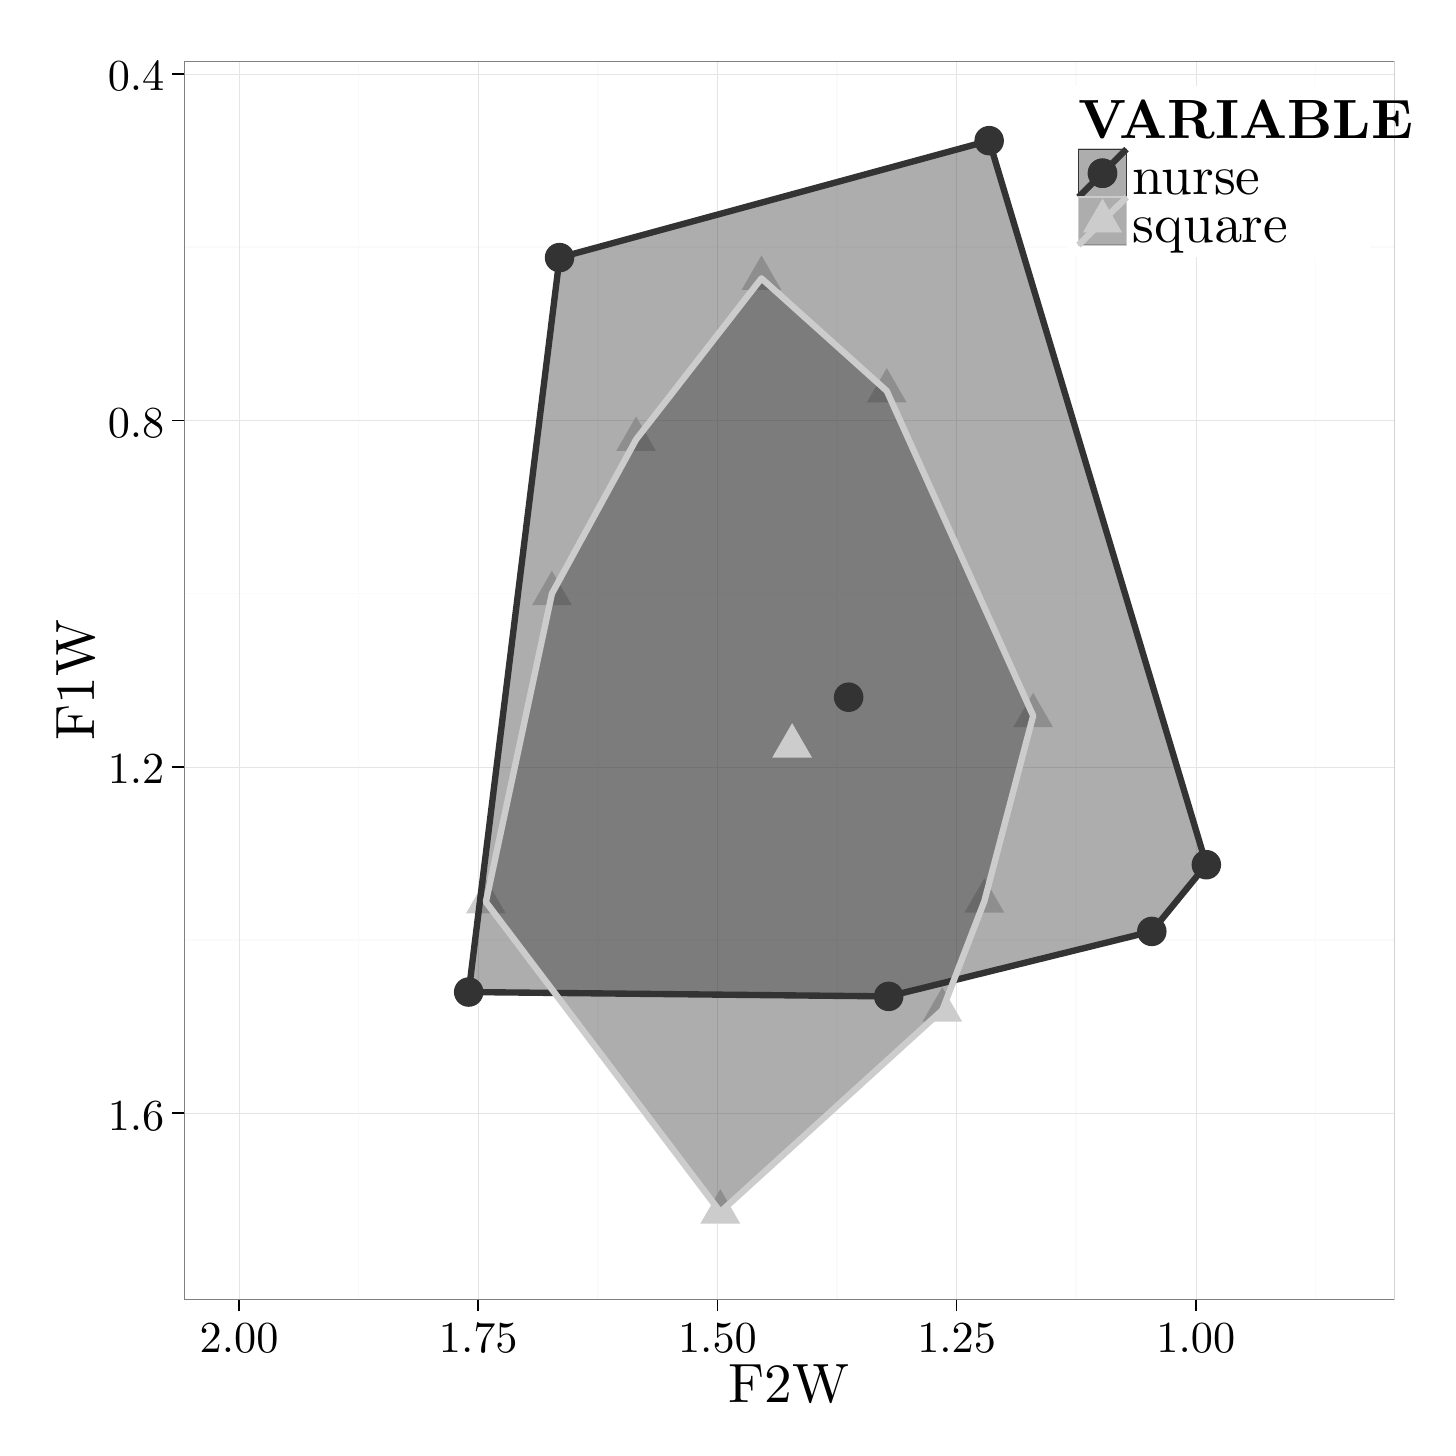
\begin{tikzpicture}[x=1pt,y=1pt]
\definecolor{fillColor}{RGB}{255,255,255}
\path[use as bounding box,fill=fillColor,fill opacity=0.00] (0,0) rectangle (505.89,505.89);
\begin{scope}
\path[clip] (  0.00,  0.00) rectangle (505.89,505.89);
\definecolor{drawColor}{RGB}{255,255,255}
\definecolor{fillColor}{RGB}{255,255,255}

\path[draw=drawColor,line width= 0.6pt,line join=round,line cap=round,fill=fillColor] (  0.00, -0.00) rectangle (505.89,505.89);
\end{scope}
\begin{scope}
\path[clip] ( 56.50, 46.31) rectangle (493.85,493.84);
\definecolor{fillColor}{RGB}{255,255,255}

\path[fill=fillColor] ( 56.50, 46.31) rectangle (493.85,493.84);
\definecolor{drawColor}{gray}{0.98}

\path[draw=drawColor,line width= 0.6pt,line join=round] ( 56.50,426.56) --
	(493.85,426.56);

\path[draw=drawColor,line width= 0.6pt,line join=round] ( 56.50,301.37) --
	(493.85,301.37);

\path[draw=drawColor,line width= 0.6pt,line join=round] ( 56.50,176.19) --
	(493.85,176.19);

\path[draw=drawColor,line width= 0.6pt,line join=round] (465.32, 46.31) --
	(465.32,493.84);

\path[draw=drawColor,line width= 0.6pt,line join=round] (378.89, 46.31) --
	(378.89,493.84);

\path[draw=drawColor,line width= 0.6pt,line join=round] (292.46, 46.31) --
	(292.46,493.84);

\path[draw=drawColor,line width= 0.6pt,line join=round] (206.03, 46.31) --
	(206.03,493.84);

\path[draw=drawColor,line width= 0.6pt,line join=round] (119.60, 46.31) --
	(119.60,493.84);
\definecolor{drawColor}{gray}{0.90}

\path[draw=drawColor,line width= 0.2pt,line join=round] ( 56.50,489.15) --
	(493.85,489.15);

\path[draw=drawColor,line width= 0.2pt,line join=round] ( 56.50,363.97) --
	(493.85,363.97);

\path[draw=drawColor,line width= 0.2pt,line join=round] ( 56.50,238.78) --
	(493.85,238.78);

\path[draw=drawColor,line width= 0.2pt,line join=round] ( 56.50,113.59) --
	(493.85,113.59);

\path[draw=drawColor,line width= 0.2pt,line join=round] (422.11, 46.31) --
	(422.11,493.84);

\path[draw=drawColor,line width= 0.2pt,line join=round] (335.68, 46.31) --
	(335.68,493.84);

\path[draw=drawColor,line width= 0.2pt,line join=round] (249.24, 46.31) --
	(249.24,493.84);

\path[draw=drawColor,line width= 0.2pt,line join=round] (162.81, 46.31) --
	(162.81,493.84);

\path[draw=drawColor,line width= 0.2pt,line join=round] ( 76.38, 46.31) --
	( 76.38,493.84);
\definecolor{fillColor}{gray}{0.20}

\path[fill=fillColor] (192.20,422.80) circle (  5.33);

\path[fill=fillColor] (347.43,465.05) circle (  5.33);

\path[fill=fillColor] (425.91,203.42) circle (  5.33);

\path[fill=fillColor] (406.20,179.32) circle (  5.33);

\path[fill=fillColor] (311.13,155.84) circle (  5.33);

\path[fill=fillColor] (159.36,157.41) circle (  5.33);
\definecolor{fillColor}{gray}{0.80}

\path[fill=fillColor] (189.43,309.67) --
	(196.62,297.22) --
	(182.25,297.22) --
	cycle;

\path[fill=fillColor] (219.86,365.38) --
	(227.04,352.93) --
	(212.67,352.93) --
	cycle;

\path[fill=fillColor] (265.15,423.59) --
	(272.33,411.14) --
	(257.96,411.14) --
	cycle;

\path[fill=fillColor] (310.44,382.90) --
	(317.62,370.46) --
	(303.25,370.46) --
	cycle;

\path[fill=fillColor] (363.33,265.54) --
	(370.52,253.10) --
	(356.15,253.10) --
	cycle;

\path[fill=fillColor] (345.70,198.57) --
	(352.89,186.12) --
	(338.52,186.12) --
	cycle;

\path[fill=fillColor] (330.49,159.13) --
	(337.68,146.69) --
	(323.31,146.69) --
	cycle;

\path[fill=fillColor] (250.28, 86.21) --
	(257.47, 73.77) --
	(243.10, 73.77) --
	cycle;

\path[fill=fillColor] (165.58,198.25) --
	(172.76,185.81) --
	(158.39,185.81) --
	cycle;
\definecolor{drawColor}{gray}{0.20}
\definecolor{fillColor}{RGB}{51,51,51}

\path[draw=drawColor,line width= 2.3pt,line join=round,line cap=round,fill=fillColor,fill opacity=0.40] (192.20,422.80) --
	(347.43,465.05) --
	(425.91,203.42) --
	(406.20,179.32) --
	(311.13,155.84) --
	(159.36,157.41) --
	cycle;
\definecolor{drawColor}{gray}{0.80}

\path[draw=drawColor,line width= 2.3pt,line join=round,line cap=round,fill=fillColor,fill opacity=0.40] (189.43,301.37) --
	(219.86,357.08) --
	(265.15,415.29) --
	(310.44,374.61) --
	(363.33,257.24) --
	(345.70,190.27) --
	(330.49,150.84) --
	(250.28, 77.92) --
	(165.58,189.96) --
	cycle;
\definecolor{fillColor}{gray}{0.20}

\path[fill=fillColor] (296.66,263.95) circle (  5.33);
\definecolor{fillColor}{gray}{0.80}

\path[fill=fillColor] (276.23,254.58) --
	(283.42,242.14) --
	(269.05,242.14) --
	cycle;
\definecolor{drawColor}{gray}{0.50}

\path[draw=drawColor,line width= 0.6pt,line join=round,line cap=round] ( 56.50, 46.31) rectangle (493.85,493.84);
\end{scope}
\begin{scope}
\path[clip] (  0.00,  0.00) rectangle (505.89,505.89);
\definecolor{drawColor}{RGB}{0,0,0}

\node[text=drawColor,anchor=base east,inner sep=0pt, outer sep=0pt, scale=  1.60] at ( 49.39,483.12) {0.4};

\node[text=drawColor,anchor=base east,inner sep=0pt, outer sep=0pt, scale=  1.60] at ( 49.39,357.93) {0.8};

\node[text=drawColor,anchor=base east,inner sep=0pt, outer sep=0pt, scale=  1.60] at ( 49.39,232.75) {1.2};

\node[text=drawColor,anchor=base east,inner sep=0pt, outer sep=0pt, scale=  1.60] at ( 49.39,107.56) {1.6};
\end{scope}
\begin{scope}
\path[clip] (  0.00,  0.00) rectangle (505.89,505.89);
\definecolor{drawColor}{RGB}{0,0,0}

\path[draw=drawColor,line width= 0.6pt,line join=round] ( 52.24,489.15) --
	( 56.50,489.15);

\path[draw=drawColor,line width= 0.6pt,line join=round] ( 52.24,363.97) --
	( 56.50,363.97);

\path[draw=drawColor,line width= 0.6pt,line join=round] ( 52.24,238.78) --
	( 56.50,238.78);

\path[draw=drawColor,line width= 0.6pt,line join=round] ( 52.24,113.59) --
	( 56.50,113.59);
\end{scope}
\begin{scope}
\path[clip] (  0.00,  0.00) rectangle (505.89,505.89);
\definecolor{drawColor}{RGB}{0,0,0}

\path[draw=drawColor,line width= 0.6pt,line join=round] (422.11, 42.04) --
	(422.11, 46.31);

\path[draw=drawColor,line width= 0.6pt,line join=round] (335.68, 42.04) --
	(335.68, 46.31);

\path[draw=drawColor,line width= 0.6pt,line join=round] (249.24, 42.04) --
	(249.24, 46.31);

\path[draw=drawColor,line width= 0.6pt,line join=round] (162.81, 42.04) --
	(162.81, 46.31);

\path[draw=drawColor,line width= 0.6pt,line join=round] ( 76.38, 42.04) --
	( 76.38, 46.31);
\end{scope}
\begin{scope}
\path[clip] (  0.00,  0.00) rectangle (505.89,505.89);
\definecolor{drawColor}{RGB}{0,0,0}

\node[text=drawColor,anchor=base,inner sep=0pt, outer sep=0pt, scale=  1.60] at (422.11, 27.13) {1.00};

\node[text=drawColor,anchor=base,inner sep=0pt, outer sep=0pt, scale=  1.60] at (335.68, 27.13) {1.25};

\node[text=drawColor,anchor=base,inner sep=0pt, outer sep=0pt, scale=  1.60] at (249.24, 27.13) {1.50};

\node[text=drawColor,anchor=base,inner sep=0pt, outer sep=0pt, scale=  1.60] at (162.81, 27.13) {1.75};

\node[text=drawColor,anchor=base,inner sep=0pt, outer sep=0pt, scale=  1.60] at ( 76.38, 27.13) {2.00};
\end{scope}
\begin{scope}
\path[clip] (  0.00,  0.00) rectangle (505.89,505.89);
\definecolor{drawColor}{RGB}{0,0,0}

\node[text=drawColor,anchor=base,inner sep=0pt, outer sep=0pt, scale=  2.00] at (275.17,  9.03) {F2W};
\end{scope}
\begin{scope}
\path[clip] (  0.00,  0.00) rectangle (505.89,505.89);
\definecolor{drawColor}{RGB}{0,0,0}

\node[text=drawColor,rotate= 90.00,anchor=base,inner sep=0pt, outer sep=0pt, scale=  2.00] at ( 24.12,270.08) {F1W};
\end{scope}
\begin{scope}
\path[clip] (  0.00,  0.00) rectangle (505.89,505.89);
\definecolor{fillColor}{RGB}{255,255,255}

\path[fill=fillColor] (375.44,423.00) rectangle (484.98,484.98);
\end{scope}
\begin{scope}
\path[clip] (  0.00,  0.00) rectangle (505.89,505.89);
\definecolor{drawColor}{RGB}{0,0,0}

\node[text=drawColor,anchor=base west,inner sep=0pt, outer sep=0pt, scale=  2.00] at (379.71,465.96) {\bfseries VARIABLE};
\end{scope}
\begin{scope}
\path[clip] (  0.00,  0.00) rectangle (505.89,505.89);
\definecolor{drawColor}{gray}{0.80}
\definecolor{fillColor}{RGB}{255,255,255}

\path[draw=drawColor,line width= 0.6pt,line join=round,line cap=round,fill=fillColor] (379.71,444.61) rectangle (397.06,461.96);
\end{scope}
\begin{scope}
\path[clip] (  0.00,  0.00) rectangle (505.89,505.89);
\definecolor{fillColor}{gray}{0.20}

\path[fill=fillColor] (388.38,453.29) circle (  5.33);
\end{scope}
\begin{scope}
\path[clip] (  0.00,  0.00) rectangle (505.89,505.89);
\definecolor{drawColor}{gray}{0.20}
\definecolor{fillColor}{RGB}{51,51,51}

\path[draw=drawColor,line width= 0.4pt,line join=round,line cap=round,fill=fillColor,fill opacity=0.40] (379.71,444.61) rectangle (397.06,461.96);

\path[draw=drawColor,line width= 2.3pt,line join=round] (379.71,444.61) --
	(397.06,461.96);
\end{scope}
\begin{scope}
\path[clip] (  0.00,  0.00) rectangle (505.89,505.89);
\definecolor{fillColor}{gray}{0.20}

\path[fill=fillColor] (388.38,453.29) circle (  5.33);
\end{scope}
\begin{scope}
\path[clip] (  0.00,  0.00) rectangle (505.89,505.89);
\definecolor{drawColor}{gray}{0.80}
\definecolor{fillColor}{RGB}{255,255,255}

\path[draw=drawColor,line width= 0.6pt,line join=round,line cap=round,fill=fillColor] (379.71,427.27) rectangle (397.06,444.61);
\end{scope}
\begin{scope}
\path[clip] (  0.00,  0.00) rectangle (505.89,505.89);
\definecolor{fillColor}{gray}{0.80}

\path[fill=fillColor] (388.38,444.24) --
	(395.57,431.79) --
	(381.20,431.79) --
	cycle;
\end{scope}
\begin{scope}
\path[clip] (  0.00,  0.00) rectangle (505.89,505.89);
\definecolor{drawColor}{gray}{0.80}
\definecolor{fillColor}{RGB}{51,51,51}

\path[draw=drawColor,line width= 0.4pt,line join=round,line cap=round,fill=fillColor,fill opacity=0.40] (379.71,427.27) rectangle (397.06,444.61);

\path[draw=drawColor,line width= 2.3pt,line join=round] (379.71,427.27) --
	(397.06,444.61);
\end{scope}
\begin{scope}
\path[clip] (  0.00,  0.00) rectangle (505.89,505.89);
\definecolor{fillColor}{gray}{0.80}

\path[fill=fillColor] (388.38,444.24) --
	(395.57,431.79) --
	(381.20,431.79) --
	cycle;
\end{scope}
\begin{scope}
\path[clip] (  0.00,  0.00) rectangle (505.89,505.89);
\definecolor{drawColor}{RGB}{0,0,0}

\node[text=drawColor,anchor=base west,inner sep=0pt, outer sep=0pt, scale=  2.00] at (399.22,445.75) {nurse};
\end{scope}
\begin{scope}
\path[clip] (  0.00,  0.00) rectangle (505.89,505.89);
\definecolor{drawColor}{RGB}{0,0,0}

\node[text=drawColor,anchor=base west,inner sep=0pt, outer sep=0pt, scale=  2.00] at (399.22,428.40) {square};
\end{scope}
\end{tikzpicture}
} 
		\caption{spontaneous speech}
		\label{fig.nurse.space.old.free}
	\end{subfigure}
	\begin{subfigure}{.49\textwidth}
		\centering
			\definecolor{shadecolor}{rgb}{0.969, 0.969, 0.969}
			\resizebox{\linewidth}{!}{% Created by tikzDevice version 0.8.1 on 2016-02-09 02:15:22
% !TEX encoding = UTF-8 Unicode
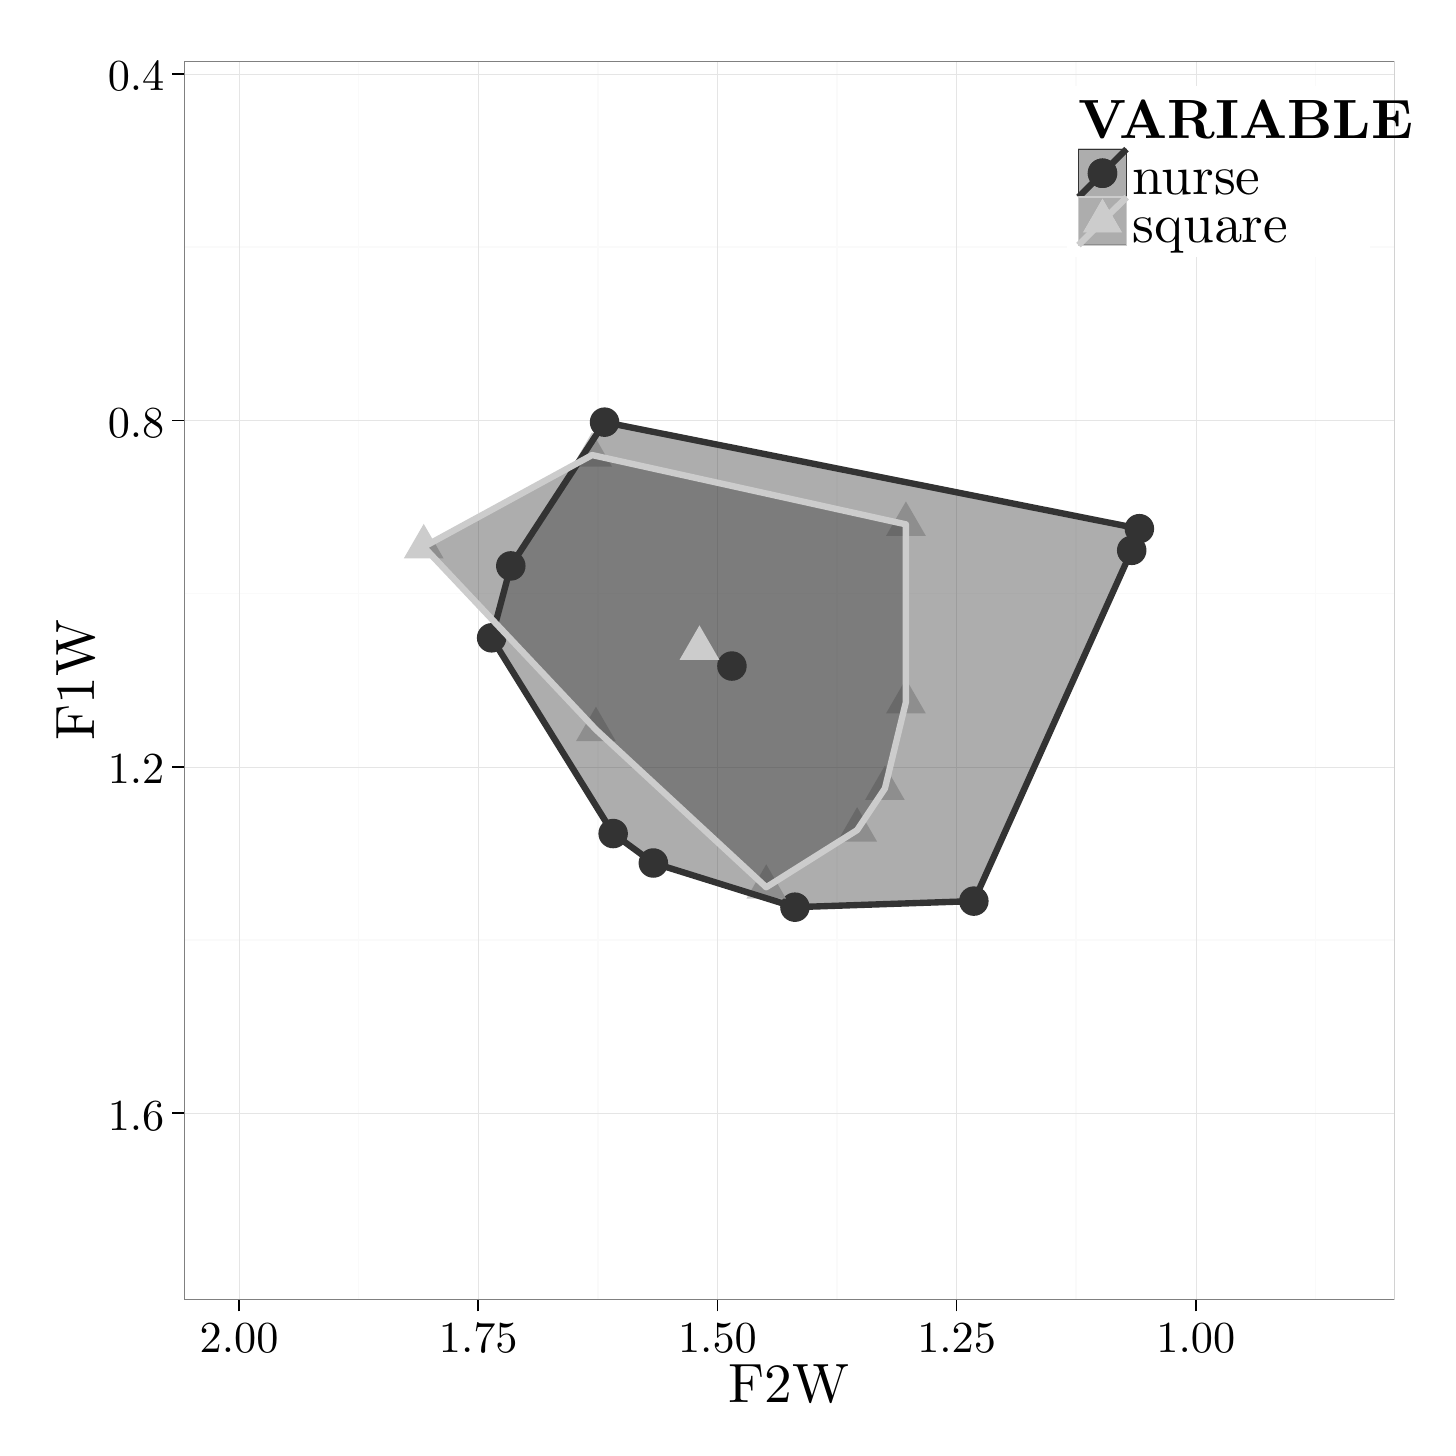
\begin{tikzpicture}[x=1pt,y=1pt]
\definecolor{fillColor}{RGB}{255,255,255}
\path[use as bounding box,fill=fillColor,fill opacity=0.00] (0,0) rectangle (505.89,505.89);
\begin{scope}
\path[clip] (  0.00,  0.00) rectangle (505.89,505.89);
\definecolor{drawColor}{RGB}{255,255,255}
\definecolor{fillColor}{RGB}{255,255,255}

\path[draw=drawColor,line width= 0.6pt,line join=round,line cap=round,fill=fillColor] (  0.00, -0.00) rectangle (505.89,505.89);
\end{scope}
\begin{scope}
\path[clip] ( 56.50, 46.31) rectangle (493.85,493.84);
\definecolor{fillColor}{RGB}{255,255,255}

\path[fill=fillColor] ( 56.50, 46.31) rectangle (493.85,493.84);
\definecolor{drawColor}{gray}{0.98}

\path[draw=drawColor,line width= 0.6pt,line join=round] ( 56.50,426.56) --
	(493.85,426.56);

\path[draw=drawColor,line width= 0.6pt,line join=round] ( 56.50,301.37) --
	(493.85,301.37);

\path[draw=drawColor,line width= 0.6pt,line join=round] ( 56.50,176.19) --
	(493.85,176.19);

\path[draw=drawColor,line width= 0.6pt,line join=round] (465.32, 46.31) --
	(465.32,493.84);

\path[draw=drawColor,line width= 0.6pt,line join=round] (378.89, 46.31) --
	(378.89,493.84);

\path[draw=drawColor,line width= 0.6pt,line join=round] (292.46, 46.31) --
	(292.46,493.84);

\path[draw=drawColor,line width= 0.6pt,line join=round] (206.03, 46.31) --
	(206.03,493.84);

\path[draw=drawColor,line width= 0.6pt,line join=round] (119.60, 46.31) --
	(119.60,493.84);
\definecolor{drawColor}{gray}{0.90}

\path[draw=drawColor,line width= 0.2pt,line join=round] ( 56.50,489.15) --
	(493.85,489.15);

\path[draw=drawColor,line width= 0.2pt,line join=round] ( 56.50,363.97) --
	(493.85,363.97);

\path[draw=drawColor,line width= 0.2pt,line join=round] ( 56.50,238.78) --
	(493.85,238.78);

\path[draw=drawColor,line width= 0.2pt,line join=round] ( 56.50,113.59) --
	(493.85,113.59);

\path[draw=drawColor,line width= 0.2pt,line join=round] (422.11, 46.31) --
	(422.11,493.84);

\path[draw=drawColor,line width= 0.2pt,line join=round] (335.68, 46.31) --
	(335.68,493.84);

\path[draw=drawColor,line width= 0.2pt,line join=round] (249.24, 46.31) --
	(249.24,493.84);

\path[draw=drawColor,line width= 0.2pt,line join=round] (162.81, 46.31) --
	(162.81,493.84);

\path[draw=drawColor,line width= 0.2pt,line join=round] ( 76.38, 46.31) --
	( 76.38,493.84);
\definecolor{fillColor}{gray}{0.20}

\path[fill=fillColor] (167.65,285.41) circle (  5.33);

\path[fill=fillColor] (174.57,311.39) circle (  5.33);

\path[fill=fillColor] (208.45,363.34) circle (  5.33);

\path[fill=fillColor] (401.71,324.84) circle (  5.33);

\path[fill=fillColor] (398.94,317.02) circle (  5.33);

\path[fill=fillColor] (341.90,190.27) circle (  5.33);

\path[fill=fillColor] (277.25,188.08) circle (  5.33);

\path[fill=fillColor] (226.08,204.04) circle (  5.33);

\path[fill=fillColor] (211.56,214.68) circle (  5.33);
\definecolor{fillColor}{gray}{0.80}

\path[fill=fillColor] (143.11,326.57) --
	(150.29,314.12) --
	(135.92,314.12) --
	cycle;

\path[fill=fillColor] (203.96,359.74) --
	(211.14,347.30) --
	(196.77,347.30) --
	cycle;

\path[fill=fillColor] (317.35,334.71) --
	(324.54,322.26) --
	(310.17,322.26) --
	cycle;

\path[fill=fillColor] (317.35,270.55) --
	(324.54,258.10) --
	(310.17,258.10) --
	cycle;

\path[fill=fillColor] (309.75,239.25) --
	(316.93,226.81) --
	(302.56,226.81) --
	cycle;

\path[fill=fillColor] (299.72,224.23) --
	(306.91,211.79) --
	(292.54,211.79) --
	cycle;

\path[fill=fillColor] (266.88,203.57) --
	(274.06,191.13) --
	(259.69,191.13) --
	cycle;

\path[fill=fillColor] (205.34,260.53) --
	(212.52,248.09) --
	(198.15,248.09) --
	cycle;
\definecolor{drawColor}{gray}{0.20}
\definecolor{fillColor}{RGB}{51,51,51}

\path[draw=drawColor,line width= 2.3pt,line join=round,line cap=round,fill=fillColor,fill opacity=0.40] (167.65,285.41) --
	(174.57,311.39) --
	(208.45,363.34) --
	(401.71,324.84) --
	(398.94,317.02) --
	(341.90,190.27) --
	(277.25,188.08) --
	(226.08,204.04) --
	(211.56,214.68) --
	cycle;
\definecolor{drawColor}{gray}{0.80}

\path[draw=drawColor,line width= 2.3pt,line join=round,line cap=round,fill=fillColor,fill opacity=0.40] (143.11,318.27) --
	(203.96,351.45) --
	(317.35,326.41) --
	(317.35,262.25) --
	(309.75,230.96) --
	(299.72,215.93) --
	(266.88,195.28) --
	(205.34,252.24) --
	cycle;
\definecolor{fillColor}{gray}{0.20}

\path[fill=fillColor] (254.48,275.21) circle (  5.33);
\definecolor{fillColor}{gray}{0.80}

\path[fill=fillColor] (242.75,289.91) --
	(249.94,277.47) --
	(235.57,277.47) --
	cycle;
\definecolor{drawColor}{gray}{0.50}

\path[draw=drawColor,line width= 0.6pt,line join=round,line cap=round] ( 56.50, 46.31) rectangle (493.85,493.84);
\end{scope}
\begin{scope}
\path[clip] (  0.00,  0.00) rectangle (505.89,505.89);
\definecolor{drawColor}{RGB}{0,0,0}

\node[text=drawColor,anchor=base east,inner sep=0pt, outer sep=0pt, scale=  1.60] at ( 49.39,483.12) {0.4};

\node[text=drawColor,anchor=base east,inner sep=0pt, outer sep=0pt, scale=  1.60] at ( 49.39,357.93) {0.8};

\node[text=drawColor,anchor=base east,inner sep=0pt, outer sep=0pt, scale=  1.60] at ( 49.39,232.75) {1.2};

\node[text=drawColor,anchor=base east,inner sep=0pt, outer sep=0pt, scale=  1.60] at ( 49.39,107.56) {1.6};
\end{scope}
\begin{scope}
\path[clip] (  0.00,  0.00) rectangle (505.89,505.89);
\definecolor{drawColor}{RGB}{0,0,0}

\path[draw=drawColor,line width= 0.6pt,line join=round] ( 52.24,489.15) --
	( 56.50,489.15);

\path[draw=drawColor,line width= 0.6pt,line join=round] ( 52.24,363.97) --
	( 56.50,363.97);

\path[draw=drawColor,line width= 0.6pt,line join=round] ( 52.24,238.78) --
	( 56.50,238.78);

\path[draw=drawColor,line width= 0.6pt,line join=round] ( 52.24,113.59) --
	( 56.50,113.59);
\end{scope}
\begin{scope}
\path[clip] (  0.00,  0.00) rectangle (505.89,505.89);
\definecolor{drawColor}{RGB}{0,0,0}

\path[draw=drawColor,line width= 0.6pt,line join=round] (422.11, 42.04) --
	(422.11, 46.31);

\path[draw=drawColor,line width= 0.6pt,line join=round] (335.68, 42.04) --
	(335.68, 46.31);

\path[draw=drawColor,line width= 0.6pt,line join=round] (249.24, 42.04) --
	(249.24, 46.31);

\path[draw=drawColor,line width= 0.6pt,line join=round] (162.81, 42.04) --
	(162.81, 46.31);

\path[draw=drawColor,line width= 0.6pt,line join=round] ( 76.38, 42.04) --
	( 76.38, 46.31);
\end{scope}
\begin{scope}
\path[clip] (  0.00,  0.00) rectangle (505.89,505.89);
\definecolor{drawColor}{RGB}{0,0,0}

\node[text=drawColor,anchor=base,inner sep=0pt, outer sep=0pt, scale=  1.60] at (422.11, 27.13) {1.00};

\node[text=drawColor,anchor=base,inner sep=0pt, outer sep=0pt, scale=  1.60] at (335.68, 27.13) {1.25};

\node[text=drawColor,anchor=base,inner sep=0pt, outer sep=0pt, scale=  1.60] at (249.24, 27.13) {1.50};

\node[text=drawColor,anchor=base,inner sep=0pt, outer sep=0pt, scale=  1.60] at (162.81, 27.13) {1.75};

\node[text=drawColor,anchor=base,inner sep=0pt, outer sep=0pt, scale=  1.60] at ( 76.38, 27.13) {2.00};
\end{scope}
\begin{scope}
\path[clip] (  0.00,  0.00) rectangle (505.89,505.89);
\definecolor{drawColor}{RGB}{0,0,0}

\node[text=drawColor,anchor=base,inner sep=0pt, outer sep=0pt, scale=  2.00] at (275.17,  9.03) {F2W};
\end{scope}
\begin{scope}
\path[clip] (  0.00,  0.00) rectangle (505.89,505.89);
\definecolor{drawColor}{RGB}{0,0,0}

\node[text=drawColor,rotate= 90.00,anchor=base,inner sep=0pt, outer sep=0pt, scale=  2.00] at ( 24.12,270.08) {F1W};
\end{scope}
\begin{scope}
\path[clip] (  0.00,  0.00) rectangle (505.89,505.89);
\definecolor{fillColor}{RGB}{255,255,255}

\path[fill=fillColor] (375.44,423.00) rectangle (484.98,484.98);
\end{scope}
\begin{scope}
\path[clip] (  0.00,  0.00) rectangle (505.89,505.89);
\definecolor{drawColor}{RGB}{0,0,0}

\node[text=drawColor,anchor=base west,inner sep=0pt, outer sep=0pt, scale=  2.00] at (379.71,465.96) {\bfseries VARIABLE};
\end{scope}
\begin{scope}
\path[clip] (  0.00,  0.00) rectangle (505.89,505.89);
\definecolor{drawColor}{gray}{0.80}
\definecolor{fillColor}{RGB}{255,255,255}

\path[draw=drawColor,line width= 0.6pt,line join=round,line cap=round,fill=fillColor] (379.71,444.61) rectangle (397.06,461.96);
\end{scope}
\begin{scope}
\path[clip] (  0.00,  0.00) rectangle (505.89,505.89);
\definecolor{fillColor}{gray}{0.20}

\path[fill=fillColor] (388.38,453.29) circle (  5.33);
\end{scope}
\begin{scope}
\path[clip] (  0.00,  0.00) rectangle (505.89,505.89);
\definecolor{drawColor}{gray}{0.20}
\definecolor{fillColor}{RGB}{51,51,51}

\path[draw=drawColor,line width= 0.4pt,line join=round,line cap=round,fill=fillColor,fill opacity=0.40] (379.71,444.61) rectangle (397.06,461.96);

\path[draw=drawColor,line width= 2.3pt,line join=round] (379.71,444.61) --
	(397.06,461.96);
\end{scope}
\begin{scope}
\path[clip] (  0.00,  0.00) rectangle (505.89,505.89);
\definecolor{fillColor}{gray}{0.20}

\path[fill=fillColor] (388.38,453.29) circle (  5.33);
\end{scope}
\begin{scope}
\path[clip] (  0.00,  0.00) rectangle (505.89,505.89);
\definecolor{drawColor}{gray}{0.80}
\definecolor{fillColor}{RGB}{255,255,255}

\path[draw=drawColor,line width= 0.6pt,line join=round,line cap=round,fill=fillColor] (379.71,427.27) rectangle (397.06,444.61);
\end{scope}
\begin{scope}
\path[clip] (  0.00,  0.00) rectangle (505.89,505.89);
\definecolor{fillColor}{gray}{0.80}

\path[fill=fillColor] (388.38,444.24) --
	(395.57,431.79) --
	(381.20,431.79) --
	cycle;
\end{scope}
\begin{scope}
\path[clip] (  0.00,  0.00) rectangle (505.89,505.89);
\definecolor{drawColor}{gray}{0.80}
\definecolor{fillColor}{RGB}{51,51,51}

\path[draw=drawColor,line width= 0.4pt,line join=round,line cap=round,fill=fillColor,fill opacity=0.40] (379.71,427.27) rectangle (397.06,444.61);

\path[draw=drawColor,line width= 2.3pt,line join=round] (379.71,427.27) --
	(397.06,444.61);
\end{scope}
\begin{scope}
\path[clip] (  0.00,  0.00) rectangle (505.89,505.89);
\definecolor{fillColor}{gray}{0.80}

\path[fill=fillColor] (388.38,444.24) --
	(395.57,431.79) --
	(381.20,431.79) --
	cycle;
\end{scope}
\begin{scope}
\path[clip] (  0.00,  0.00) rectangle (505.89,505.89);
\definecolor{drawColor}{RGB}{0,0,0}

\node[text=drawColor,anchor=base west,inner sep=0pt, outer sep=0pt, scale=  2.00] at (399.22,445.75) {nurse};
\end{scope}
\begin{scope}
\path[clip] (  0.00,  0.00) rectangle (505.89,505.89);
\definecolor{drawColor}{RGB}{0,0,0}

\node[text=drawColor,anchor=base west,inner sep=0pt, outer sep=0pt, scale=  2.00] at (399.22,428.40) {square};
\end{scope}
\end{tikzpicture}
} 
		\caption{accent performance}
		\label{fig.nurse.space.old.imit}
	\end{subfigure}
	
	\caption{\textsc{nurse}-\textsc{square}: vowel space by style (old speakers)}
	\label{fig.nurse.space.old}
\end{figure}

It still does make sense to have a closer look at the individual distributions.
\isi{Pillai} scores allow statements about the degree of overlap between two distributions, but they say nothing about the exact shape, the location, or the centre of gravity of these distributions.
Figure \ref{fig.nurse.space.old} represents the realisational spaces of \textsc{nurse} and \textsc{square} in the different styles for the oldest speakers in the sample.
Here and in Figures \ref{fig.nurse.space.mid} and \ref{fig.nurse.space.young} the vowel spaces that \textsc{nurse} occurs in are marked by the dark, that of \textsc{square} by the light polygons.
The mean realisations are represented by circles (\textsc{nurse}) and triangles (\textsc{square}) of the respective shades.

Two aspects strike the observer when inspecting the realisational spaces of these two vowels in the old generation:
\begin{inparaenum}[(1)]
	\item The range of variation (as represented by the surface area of the polygons) increases considerably from the word list to free speech, via accent imitation\is{accent performance} and the reading passage.
	\item The vertical extent of the polygons is much larger than the horizontal one, which means variants of both \textsc{nurse} and \textsc{square} are relatively stable in the front-back dimension.
\end{inparaenum}
It is possible that the large degree of homogeneity that is found for the word list is primarily due to the smaller number of observations in this sub-sample; if more data are collected (like for the free speech style in this study) the chance of including the occasional `extreme' variant increases.
It seems more likely, however, that subjects largely agree on which variants are appropriate for the more formal registers reading and word list (and, incidentally, also for the \isi{stereotype} of Scouse!), but allow themselves to choose from a larger set of options in spontaneous speech.
These options (in free speech and the other styles) seem to differ largely in F1, but a lot less so in F2.
With the possible exception of Figure \ref{fig.nurse.space.old.imit} vowel spaces are all larger in height than width, which indicates that the old speakers in my sample manipulate F1 quite considerably for these vowels, while producing all variants with a relatively stable F2.

When we look at the mean realisations of the two vowels (dark circle for \textsc{nurse}, light triangle for \textsc{square} in the centre of the polygon) in this age group, we can, first of all, see that the distance between the centres of gravity is greatest in Figure \ref{fig.nurse.space.old.free}, which means that the higher \isi{Pillai} score and lower p-value found for this sub-sample (cf. Table \ref{tab.pillai.nurse.agestyle}) is \emph{not} only due to the larger number of observations in this style, after all.
The distributions are indeed more distinct\is{distinctness} than in the other registers, if only slightly so.
The relative positioning of mean vowel realisations is as would be expected: \textsc{nurse} is both slightly higher and more central than \textsc{square}.
Interestingly now, the mean of \textsc{nurse} does not really move at all from spontaneous speech to the reading passage (Figure \ref{fig.nurse.space.old.read}).
All the same, the average realisations of the two vowels actually become more similar (instead of more distinct\is{distinctness}, as would be expected for a more formal register), because \textsc{square} is both raised and centralised and thus approaches \textsc{nurse}.
For the word list (Figure \ref{fig.nurse.space.old.list}), both means are somewhat lowered and even closer to each other.
This is, for \textsc{nurse} at least, again contrary to expectations, since a move towards more standard realisations would involve raising rather than lowering.
Only when we move from free speech to accent imitation\is{accent performance} (Figures \ref{fig.nurse.space.old.free} and \ref{fig.nurse.space.old.imit}), does the mean of \textsc{nurse} change more drastically: it is considerably more front, and almost identical to \textsc{square}, which is fronted and raised as well.

\subsubsection{Middle-aged speakers}

\begin{figure}[h!]
	\centering
	\begin{subfigure}{.49\textwidth}
		\centering
			\definecolor{shadecolor}{rgb}{0.969, 0.969, 0.969}
			\resizebox{\linewidth}{!}{% Created by tikzDevice version 0.8.1 on 2016-02-09 02:15:23
% !TEX encoding = UTF-8 Unicode
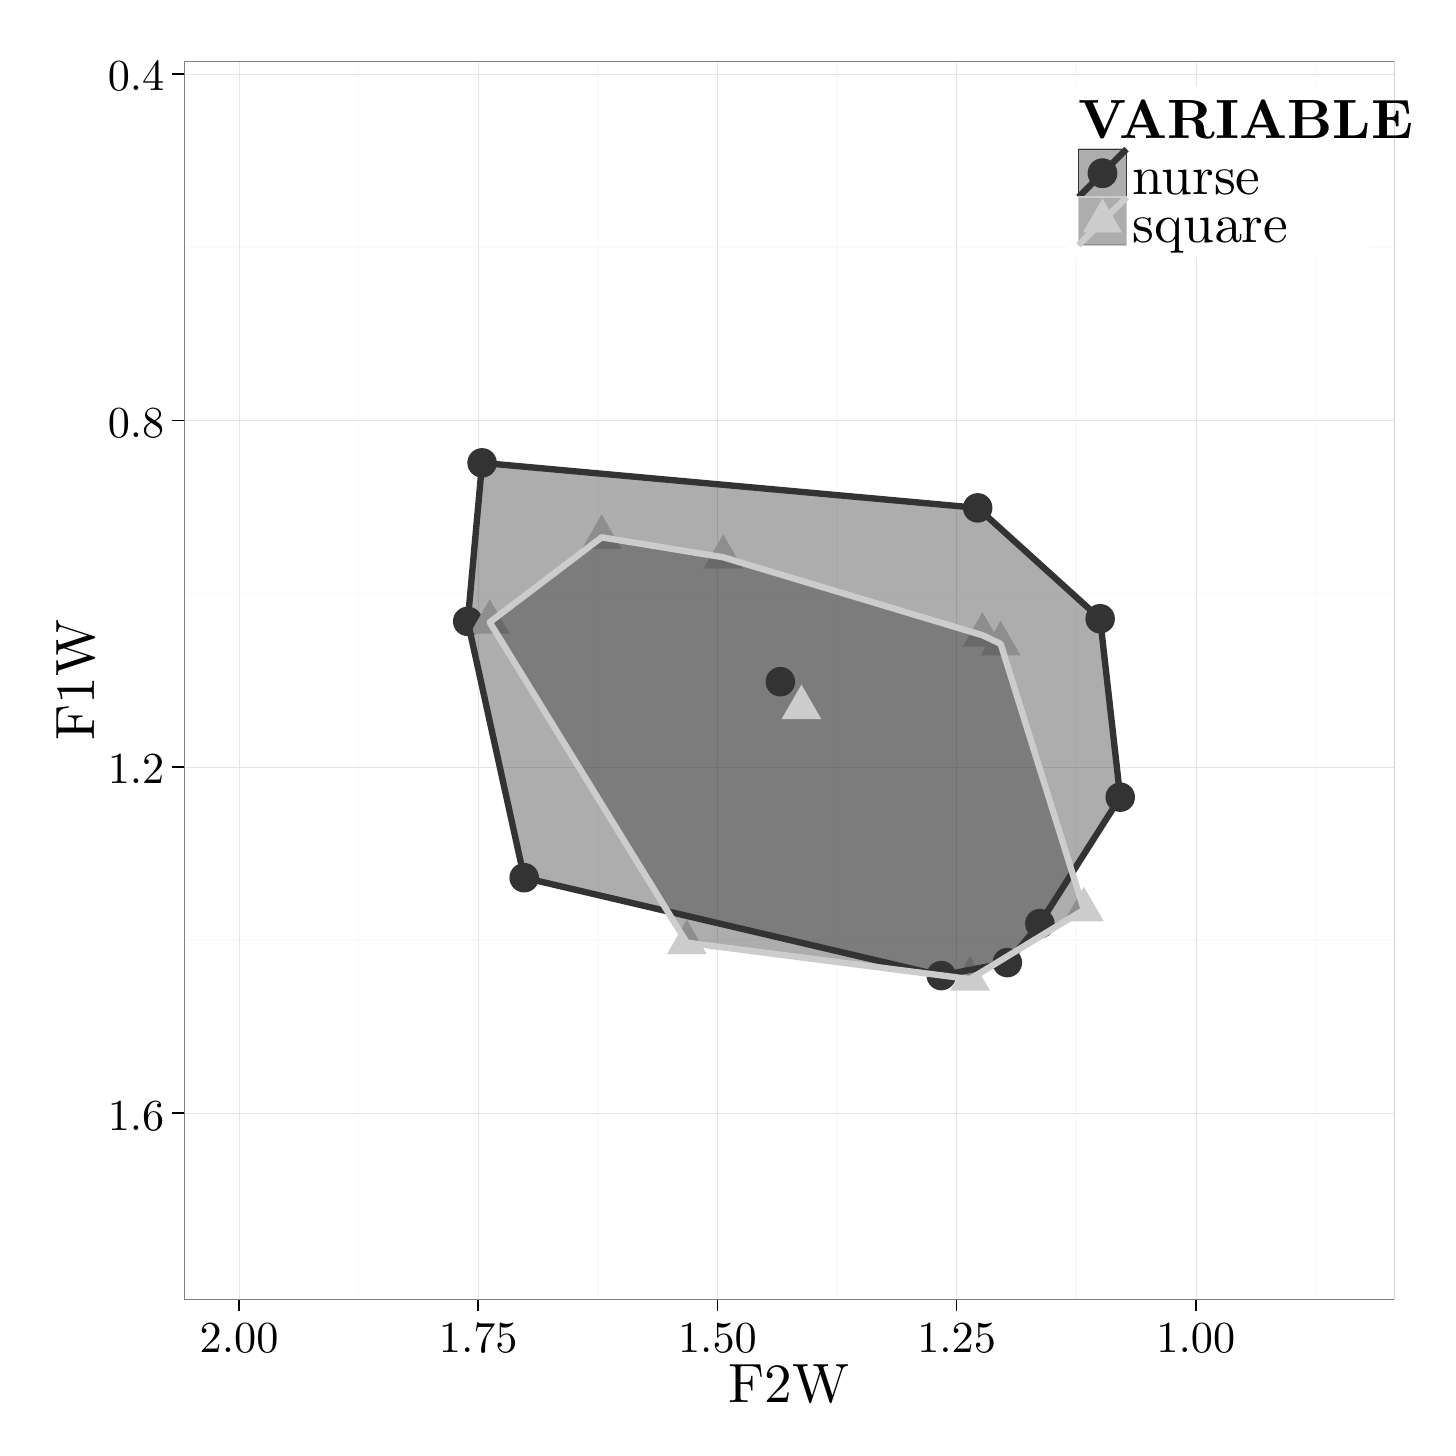
\begin{tikzpicture}[x=1pt,y=1pt]
\definecolor{fillColor}{RGB}{255,255,255}
\path[use as bounding box,fill=fillColor,fill opacity=0.00] (0,0) rectangle (505.89,505.89);
\begin{scope}
\path[clip] (  0.00,  0.00) rectangle (505.89,505.89);
\definecolor{drawColor}{RGB}{255,255,255}
\definecolor{fillColor}{RGB}{255,255,255}

\path[draw=drawColor,line width= 0.6pt,line join=round,line cap=round,fill=fillColor] (  0.00, -0.00) rectangle (505.89,505.89);
\end{scope}
\begin{scope}
\path[clip] ( 56.50, 46.31) rectangle (493.85,493.84);
\definecolor{fillColor}{RGB}{255,255,255}

\path[fill=fillColor] ( 56.50, 46.31) rectangle (493.85,493.84);
\definecolor{drawColor}{gray}{0.98}

\path[draw=drawColor,line width= 0.6pt,line join=round] ( 56.50,426.56) --
	(493.85,426.56);

\path[draw=drawColor,line width= 0.6pt,line join=round] ( 56.50,301.37) --
	(493.85,301.37);

\path[draw=drawColor,line width= 0.6pt,line join=round] ( 56.50,176.19) --
	(493.85,176.19);

\path[draw=drawColor,line width= 0.6pt,line join=round] (465.32, 46.31) --
	(465.32,493.84);

\path[draw=drawColor,line width= 0.6pt,line join=round] (378.89, 46.31) --
	(378.89,493.84);

\path[draw=drawColor,line width= 0.6pt,line join=round] (292.46, 46.31) --
	(292.46,493.84);

\path[draw=drawColor,line width= 0.6pt,line join=round] (206.03, 46.31) --
	(206.03,493.84);

\path[draw=drawColor,line width= 0.6pt,line join=round] (119.60, 46.31) --
	(119.60,493.84);
\definecolor{drawColor}{gray}{0.90}

\path[draw=drawColor,line width= 0.2pt,line join=round] ( 56.50,489.15) --
	(493.85,489.15);

\path[draw=drawColor,line width= 0.2pt,line join=round] ( 56.50,363.97) --
	(493.85,363.97);

\path[draw=drawColor,line width= 0.2pt,line join=round] ( 56.50,238.78) --
	(493.85,238.78);

\path[draw=drawColor,line width= 0.2pt,line join=round] ( 56.50,113.59) --
	(493.85,113.59);

\path[draw=drawColor,line width= 0.2pt,line join=round] (422.11, 46.31) --
	(422.11,493.84);

\path[draw=drawColor,line width= 0.2pt,line join=round] (335.68, 46.31) --
	(335.68,493.84);

\path[draw=drawColor,line width= 0.2pt,line join=round] (249.24, 46.31) --
	(249.24,493.84);

\path[draw=drawColor,line width= 0.2pt,line join=round] (162.81, 46.31) --
	(162.81,493.84);

\path[draw=drawColor,line width= 0.2pt,line join=round] ( 76.38, 46.31) --
	( 76.38,493.84);
\definecolor{fillColor}{gray}{0.20}

\path[fill=fillColor] (159.01,291.36) circle (  5.33);

\path[fill=fillColor] (164.20,348.63) circle (  5.33);

\path[fill=fillColor] (343.28,332.36) circle (  5.33);

\path[fill=fillColor] (387.53,292.30) circle (  5.33);

\path[fill=fillColor] (394.79,227.83) circle (  5.33);

\path[fill=fillColor] (365.75,182.13) circle (  5.33);

\path[fill=fillColor] (354.00,168.05) circle (  5.33);

\path[fill=fillColor] (330.14,163.36) circle (  5.33);

\path[fill=fillColor] (179.41,198.72) circle (  5.33);
\definecolor{fillColor}{gray}{0.80}

\path[fill=fillColor] (166.96,299.34) --
	(174.15,286.90) --
	(159.78,286.90) --
	cycle;

\path[fill=fillColor] (207.41,330.01) --
	(214.60,317.57) --
	(200.23,317.57) --
	cycle;

\path[fill=fillColor] (251.32,322.81) --
	(258.50,310.37) --
	(244.13,310.37) --
	cycle;

\path[fill=fillColor] (345.01,294.65) --
	(352.20,282.20) --
	(337.83,282.20) --
	cycle;

\path[fill=fillColor] (351.58,291.52) --
	(358.76,279.07) --
	(344.39,279.07) --
	cycle;

\path[fill=fillColor] (381.66,195.44) --
	(388.84,182.99) --
	(374.47,182.99) --
	cycle;

\path[fill=fillColor] (340.52,170.40) --
	(347.70,157.96) --
	(333.33,157.96) --
	cycle;

\path[fill=fillColor] (238.18,183.54) --
	(245.37,171.10) --
	(231.00,171.10) --
	cycle;
\definecolor{drawColor}{gray}{0.20}
\definecolor{fillColor}{RGB}{51,51,51}

\path[draw=drawColor,line width= 2.3pt,line join=round,line cap=round,fill=fillColor,fill opacity=0.40] (159.01,291.36) --
	(164.20,348.63) --
	(343.28,332.36) --
	(387.53,292.30) --
	(394.79,227.83) --
	(365.75,182.13) --
	(354.00,168.05) --
	(330.14,163.36) --
	(179.41,198.72) --
	cycle;
\definecolor{drawColor}{gray}{0.80}

\path[draw=drawColor,line width= 2.3pt,line join=round,line cap=round,fill=fillColor,fill opacity=0.40] (166.96,291.04) --
	(207.41,321.72) --
	(251.32,314.52) --
	(345.01,286.35) --
	(351.58,283.22) --
	(381.66,187.14) --
	(340.52,162.10) --
	(238.18,175.25) --
	cycle;
\definecolor{fillColor}{gray}{0.20}

\path[fill=fillColor] (271.98,269.55) circle (  5.33);
\definecolor{fillColor}{gray}{0.80}

\path[fill=fillColor] (279.60,268.49) --
	(286.78,256.05) --
	(272.41,256.05) --
	cycle;
\definecolor{drawColor}{gray}{0.50}

\path[draw=drawColor,line width= 0.6pt,line join=round,line cap=round] ( 56.50, 46.31) rectangle (493.85,493.84);
\end{scope}
\begin{scope}
\path[clip] (  0.00,  0.00) rectangle (505.89,505.89);
\definecolor{drawColor}{RGB}{0,0,0}

\node[text=drawColor,anchor=base east,inner sep=0pt, outer sep=0pt, scale=  1.60] at ( 49.39,483.12) {0.4};

\node[text=drawColor,anchor=base east,inner sep=0pt, outer sep=0pt, scale=  1.60] at ( 49.39,357.93) {0.8};

\node[text=drawColor,anchor=base east,inner sep=0pt, outer sep=0pt, scale=  1.60] at ( 49.39,232.75) {1.2};

\node[text=drawColor,anchor=base east,inner sep=0pt, outer sep=0pt, scale=  1.60] at ( 49.39,107.56) {1.6};
\end{scope}
\begin{scope}
\path[clip] (  0.00,  0.00) rectangle (505.89,505.89);
\definecolor{drawColor}{RGB}{0,0,0}

\path[draw=drawColor,line width= 0.6pt,line join=round] ( 52.24,489.15) --
	( 56.50,489.15);

\path[draw=drawColor,line width= 0.6pt,line join=round] ( 52.24,363.97) --
	( 56.50,363.97);

\path[draw=drawColor,line width= 0.6pt,line join=round] ( 52.24,238.78) --
	( 56.50,238.78);

\path[draw=drawColor,line width= 0.6pt,line join=round] ( 52.24,113.59) --
	( 56.50,113.59);
\end{scope}
\begin{scope}
\path[clip] (  0.00,  0.00) rectangle (505.89,505.89);
\definecolor{drawColor}{RGB}{0,0,0}

\path[draw=drawColor,line width= 0.6pt,line join=round] (422.11, 42.04) --
	(422.11, 46.31);

\path[draw=drawColor,line width= 0.6pt,line join=round] (335.68, 42.04) --
	(335.68, 46.31);

\path[draw=drawColor,line width= 0.6pt,line join=round] (249.24, 42.04) --
	(249.24, 46.31);

\path[draw=drawColor,line width= 0.6pt,line join=round] (162.81, 42.04) --
	(162.81, 46.31);

\path[draw=drawColor,line width= 0.6pt,line join=round] ( 76.38, 42.04) --
	( 76.38, 46.31);
\end{scope}
\begin{scope}
\path[clip] (  0.00,  0.00) rectangle (505.89,505.89);
\definecolor{drawColor}{RGB}{0,0,0}

\node[text=drawColor,anchor=base,inner sep=0pt, outer sep=0pt, scale=  1.60] at (422.11, 27.13) {1.00};

\node[text=drawColor,anchor=base,inner sep=0pt, outer sep=0pt, scale=  1.60] at (335.68, 27.13) {1.25};

\node[text=drawColor,anchor=base,inner sep=0pt, outer sep=0pt, scale=  1.60] at (249.24, 27.13) {1.50};

\node[text=drawColor,anchor=base,inner sep=0pt, outer sep=0pt, scale=  1.60] at (162.81, 27.13) {1.75};

\node[text=drawColor,anchor=base,inner sep=0pt, outer sep=0pt, scale=  1.60] at ( 76.38, 27.13) {2.00};
\end{scope}
\begin{scope}
\path[clip] (  0.00,  0.00) rectangle (505.89,505.89);
\definecolor{drawColor}{RGB}{0,0,0}

\node[text=drawColor,anchor=base,inner sep=0pt, outer sep=0pt, scale=  2.00] at (275.17,  9.03) {F2W};
\end{scope}
\begin{scope}
\path[clip] (  0.00,  0.00) rectangle (505.89,505.89);
\definecolor{drawColor}{RGB}{0,0,0}

\node[text=drawColor,rotate= 90.00,anchor=base,inner sep=0pt, outer sep=0pt, scale=  2.00] at ( 24.12,270.08) {F1W};
\end{scope}
\begin{scope}
\path[clip] (  0.00,  0.00) rectangle (505.89,505.89);
\definecolor{fillColor}{RGB}{255,255,255}

\path[fill=fillColor] (375.44,423.00) rectangle (484.98,484.98);
\end{scope}
\begin{scope}
\path[clip] (  0.00,  0.00) rectangle (505.89,505.89);
\definecolor{drawColor}{RGB}{0,0,0}

\node[text=drawColor,anchor=base west,inner sep=0pt, outer sep=0pt, scale=  2.00] at (379.71,465.96) {\bfseries VARIABLE};
\end{scope}
\begin{scope}
\path[clip] (  0.00,  0.00) rectangle (505.89,505.89);
\definecolor{drawColor}{gray}{0.80}
\definecolor{fillColor}{RGB}{255,255,255}

\path[draw=drawColor,line width= 0.6pt,line join=round,line cap=round,fill=fillColor] (379.71,444.61) rectangle (397.06,461.96);
\end{scope}
\begin{scope}
\path[clip] (  0.00,  0.00) rectangle (505.89,505.89);
\definecolor{fillColor}{gray}{0.20}

\path[fill=fillColor] (388.38,453.29) circle (  5.33);
\end{scope}
\begin{scope}
\path[clip] (  0.00,  0.00) rectangle (505.89,505.89);
\definecolor{drawColor}{gray}{0.20}
\definecolor{fillColor}{RGB}{51,51,51}

\path[draw=drawColor,line width= 0.4pt,line join=round,line cap=round,fill=fillColor,fill opacity=0.40] (379.71,444.61) rectangle (397.06,461.96);

\path[draw=drawColor,line width= 2.3pt,line join=round] (379.71,444.61) --
	(397.06,461.96);
\end{scope}
\begin{scope}
\path[clip] (  0.00,  0.00) rectangle (505.89,505.89);
\definecolor{fillColor}{gray}{0.20}

\path[fill=fillColor] (388.38,453.29) circle (  5.33);
\end{scope}
\begin{scope}
\path[clip] (  0.00,  0.00) rectangle (505.89,505.89);
\definecolor{drawColor}{gray}{0.80}
\definecolor{fillColor}{RGB}{255,255,255}

\path[draw=drawColor,line width= 0.6pt,line join=round,line cap=round,fill=fillColor] (379.71,427.27) rectangle (397.06,444.61);
\end{scope}
\begin{scope}
\path[clip] (  0.00,  0.00) rectangle (505.89,505.89);
\definecolor{fillColor}{gray}{0.80}

\path[fill=fillColor] (388.38,444.24) --
	(395.57,431.79) --
	(381.20,431.79) --
	cycle;
\end{scope}
\begin{scope}
\path[clip] (  0.00,  0.00) rectangle (505.89,505.89);
\definecolor{drawColor}{gray}{0.80}
\definecolor{fillColor}{RGB}{51,51,51}

\path[draw=drawColor,line width= 0.4pt,line join=round,line cap=round,fill=fillColor,fill opacity=0.40] (379.71,427.27) rectangle (397.06,444.61);

\path[draw=drawColor,line width= 2.3pt,line join=round] (379.71,427.27) --
	(397.06,444.61);
\end{scope}
\begin{scope}
\path[clip] (  0.00,  0.00) rectangle (505.89,505.89);
\definecolor{fillColor}{gray}{0.80}

\path[fill=fillColor] (388.38,444.24) --
	(395.57,431.79) --
	(381.20,431.79) --
	cycle;
\end{scope}
\begin{scope}
\path[clip] (  0.00,  0.00) rectangle (505.89,505.89);
\definecolor{drawColor}{RGB}{0,0,0}

\node[text=drawColor,anchor=base west,inner sep=0pt, outer sep=0pt, scale=  2.00] at (399.22,445.75) {nurse};
\end{scope}
\begin{scope}
\path[clip] (  0.00,  0.00) rectangle (505.89,505.89);
\definecolor{drawColor}{RGB}{0,0,0}

\node[text=drawColor,anchor=base west,inner sep=0pt, outer sep=0pt, scale=  2.00] at (399.22,428.40) {square};
\end{scope}
\end{tikzpicture}
} 
		\caption{word list}
		\label{fig.nurse.space.mid.list}
	\end{subfigure}
	\begin{subfigure}{.49\textwidth}
		\centering
			\definecolor{shadecolor}{rgb}{0.969, 0.969, 0.969}
			\resizebox{\linewidth}{!}{% Created by tikzDevice version 0.8.1 on 2016-02-09 02:15:24
% !TEX encoding = UTF-8 Unicode
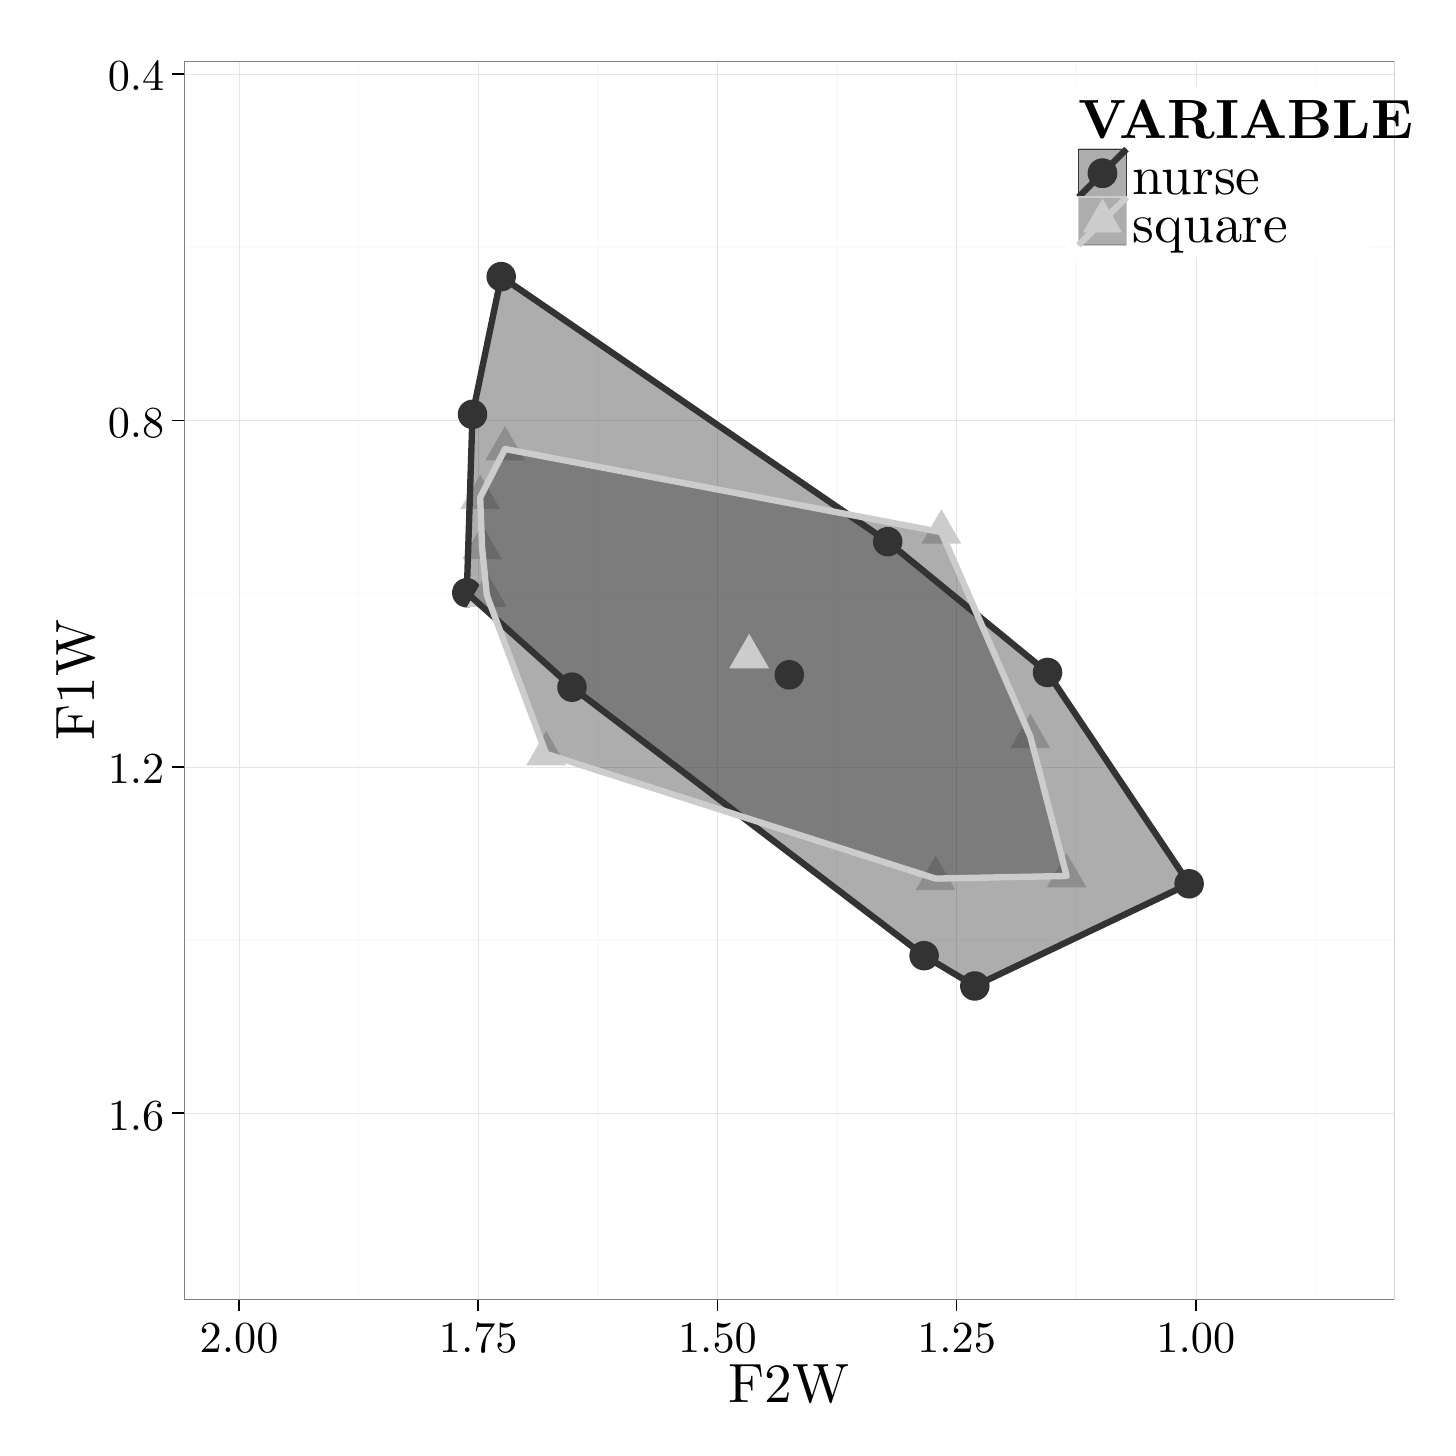
\begin{tikzpicture}[x=1pt,y=1pt]
\definecolor{fillColor}{RGB}{255,255,255}
\path[use as bounding box,fill=fillColor,fill opacity=0.00] (0,0) rectangle (505.89,505.89);
\begin{scope}
\path[clip] (  0.00,  0.00) rectangle (505.89,505.89);
\definecolor{drawColor}{RGB}{255,255,255}
\definecolor{fillColor}{RGB}{255,255,255}

\path[draw=drawColor,line width= 0.6pt,line join=round,line cap=round,fill=fillColor] (  0.00, -0.00) rectangle (505.89,505.89);
\end{scope}
\begin{scope}
\path[clip] ( 56.50, 46.31) rectangle (493.85,493.84);
\definecolor{fillColor}{RGB}{255,255,255}

\path[fill=fillColor] ( 56.50, 46.31) rectangle (493.85,493.84);
\definecolor{drawColor}{gray}{0.98}

\path[draw=drawColor,line width= 0.6pt,line join=round] ( 56.50,426.56) --
	(493.85,426.56);

\path[draw=drawColor,line width= 0.6pt,line join=round] ( 56.50,301.37) --
	(493.85,301.37);

\path[draw=drawColor,line width= 0.6pt,line join=round] ( 56.50,176.19) --
	(493.85,176.19);

\path[draw=drawColor,line width= 0.6pt,line join=round] (465.32, 46.31) --
	(465.32,493.84);

\path[draw=drawColor,line width= 0.6pt,line join=round] (378.89, 46.31) --
	(378.89,493.84);

\path[draw=drawColor,line width= 0.6pt,line join=round] (292.46, 46.31) --
	(292.46,493.84);

\path[draw=drawColor,line width= 0.6pt,line join=round] (206.03, 46.31) --
	(206.03,493.84);

\path[draw=drawColor,line width= 0.6pt,line join=round] (119.60, 46.31) --
	(119.60,493.84);
\definecolor{drawColor}{gray}{0.90}

\path[draw=drawColor,line width= 0.2pt,line join=round] ( 56.50,489.15) --
	(493.85,489.15);

\path[draw=drawColor,line width= 0.2pt,line join=round] ( 56.50,363.97) --
	(493.85,363.97);

\path[draw=drawColor,line width= 0.2pt,line join=round] ( 56.50,238.78) --
	(493.85,238.78);

\path[draw=drawColor,line width= 0.2pt,line join=round] ( 56.50,113.59) --
	(493.85,113.59);

\path[draw=drawColor,line width= 0.2pt,line join=round] (422.11, 46.31) --
	(422.11,493.84);

\path[draw=drawColor,line width= 0.2pt,line join=round] (335.68, 46.31) --
	(335.68,493.84);

\path[draw=drawColor,line width= 0.2pt,line join=round] (249.24, 46.31) --
	(249.24,493.84);

\path[draw=drawColor,line width= 0.2pt,line join=round] (162.81, 46.31) --
	(162.81,493.84);

\path[draw=drawColor,line width= 0.2pt,line join=round] ( 76.38, 46.31) --
	( 76.38,493.84);
\definecolor{fillColor}{gray}{0.20}

\path[fill=fillColor] (158.67,301.69) circle (  5.33);

\path[fill=fillColor] (160.74,366.16) circle (  5.33);

\path[fill=fillColor] (171.11,415.92) circle (  5.33);

\path[fill=fillColor] (310.78,320.15) circle (  5.33);

\path[fill=fillColor] (368.52,272.89) circle (  5.33);

\path[fill=fillColor] (419.69,196.53) circle (  5.33);

\path[fill=fillColor] (342.24,159.60) circle (  5.33);

\path[fill=fillColor] (323.92,170.55) circle (  5.33);

\path[fill=fillColor] (196.69,267.57) circle (  5.33);
\definecolor{fillColor}{gray}{0.80}

\path[fill=fillColor] (165.93,309.04) --
	(173.11,296.60) --
	(158.74,296.60) --
	cycle;

\path[fill=fillColor] (164.20,326.26) --
	(171.38,313.81) --
	(157.01,313.81) --
	cycle;

\path[fill=fillColor] (163.51,344.41) --
	(170.69,331.96) --
	(156.32,331.96) --
	cycle;

\path[fill=fillColor] (172.49,361.93) --
	(179.68,349.49) --
	(165.31,349.49) --
	cycle;

\path[fill=fillColor] (330.14,331.89) --
	(337.33,319.44) --
	(322.96,319.44) --
	cycle;

\path[fill=fillColor] (362.30,258.03) --
	(369.48,245.59) --
	(355.11,245.59) --
	cycle;

\path[fill=fillColor] (375.43,207.64) --
	(382.62,195.20) --
	(368.25,195.20) --
	cycle;

\path[fill=fillColor] (328.07,206.70) --
	(335.26,194.26) --
	(320.89,194.26) --
	cycle;

\path[fill=fillColor] (187.36,251.77) --
	(194.55,239.33) --
	(180.18,239.33) --
	cycle;
\definecolor{drawColor}{gray}{0.20}
\definecolor{fillColor}{RGB}{51,51,51}

\path[draw=drawColor,line width= 2.3pt,line join=round,line cap=round,fill=fillColor,fill opacity=0.40] (158.67,301.69) --
	(160.74,366.16) --
	(171.11,415.92) --
	(310.78,320.15) --
	(368.52,272.89) --
	(419.69,196.53) --
	(342.24,159.60) --
	(323.92,170.55) --
	(196.69,267.57) --
	cycle;
\definecolor{drawColor}{gray}{0.80}

\path[draw=drawColor,line width= 2.3pt,line join=round,line cap=round,fill=fillColor,fill opacity=0.40] (165.93,300.75) --
	(164.20,317.96) --
	(163.51,336.11) --
	(172.49,353.64) --
	(330.14,323.59) --
	(362.30,249.73) --
	(375.43,199.35) --
	(328.07,198.41) --
	(187.36,243.47) --
	cycle;
\definecolor{fillColor}{gray}{0.20}

\path[fill=fillColor] (275.21,272.05) circle (  5.33);
\definecolor{fillColor}{gray}{0.80}

\path[fill=fillColor] (260.71,286.86) --
	(267.89,274.41) --
	(253.52,274.41) --
	cycle;
\definecolor{drawColor}{gray}{0.50}

\path[draw=drawColor,line width= 0.6pt,line join=round,line cap=round] ( 56.50, 46.31) rectangle (493.85,493.84);
\end{scope}
\begin{scope}
\path[clip] (  0.00,  0.00) rectangle (505.89,505.89);
\definecolor{drawColor}{RGB}{0,0,0}

\node[text=drawColor,anchor=base east,inner sep=0pt, outer sep=0pt, scale=  1.60] at ( 49.39,483.12) {0.4};

\node[text=drawColor,anchor=base east,inner sep=0pt, outer sep=0pt, scale=  1.60] at ( 49.39,357.93) {0.8};

\node[text=drawColor,anchor=base east,inner sep=0pt, outer sep=0pt, scale=  1.60] at ( 49.39,232.75) {1.2};

\node[text=drawColor,anchor=base east,inner sep=0pt, outer sep=0pt, scale=  1.60] at ( 49.39,107.56) {1.6};
\end{scope}
\begin{scope}
\path[clip] (  0.00,  0.00) rectangle (505.89,505.89);
\definecolor{drawColor}{RGB}{0,0,0}

\path[draw=drawColor,line width= 0.6pt,line join=round] ( 52.24,489.15) --
	( 56.50,489.15);

\path[draw=drawColor,line width= 0.6pt,line join=round] ( 52.24,363.97) --
	( 56.50,363.97);

\path[draw=drawColor,line width= 0.6pt,line join=round] ( 52.24,238.78) --
	( 56.50,238.78);

\path[draw=drawColor,line width= 0.6pt,line join=round] ( 52.24,113.59) --
	( 56.50,113.59);
\end{scope}
\begin{scope}
\path[clip] (  0.00,  0.00) rectangle (505.89,505.89);
\definecolor{drawColor}{RGB}{0,0,0}

\path[draw=drawColor,line width= 0.6pt,line join=round] (422.11, 42.04) --
	(422.11, 46.31);

\path[draw=drawColor,line width= 0.6pt,line join=round] (335.68, 42.04) --
	(335.68, 46.31);

\path[draw=drawColor,line width= 0.6pt,line join=round] (249.24, 42.04) --
	(249.24, 46.31);

\path[draw=drawColor,line width= 0.6pt,line join=round] (162.81, 42.04) --
	(162.81, 46.31);

\path[draw=drawColor,line width= 0.6pt,line join=round] ( 76.38, 42.04) --
	( 76.38, 46.31);
\end{scope}
\begin{scope}
\path[clip] (  0.00,  0.00) rectangle (505.89,505.89);
\definecolor{drawColor}{RGB}{0,0,0}

\node[text=drawColor,anchor=base,inner sep=0pt, outer sep=0pt, scale=  1.60] at (422.11, 27.13) {1.00};

\node[text=drawColor,anchor=base,inner sep=0pt, outer sep=0pt, scale=  1.60] at (335.68, 27.13) {1.25};

\node[text=drawColor,anchor=base,inner sep=0pt, outer sep=0pt, scale=  1.60] at (249.24, 27.13) {1.50};

\node[text=drawColor,anchor=base,inner sep=0pt, outer sep=0pt, scale=  1.60] at (162.81, 27.13) {1.75};

\node[text=drawColor,anchor=base,inner sep=0pt, outer sep=0pt, scale=  1.60] at ( 76.38, 27.13) {2.00};
\end{scope}
\begin{scope}
\path[clip] (  0.00,  0.00) rectangle (505.89,505.89);
\definecolor{drawColor}{RGB}{0,0,0}

\node[text=drawColor,anchor=base,inner sep=0pt, outer sep=0pt, scale=  2.00] at (275.17,  9.03) {F2W};
\end{scope}
\begin{scope}
\path[clip] (  0.00,  0.00) rectangle (505.89,505.89);
\definecolor{drawColor}{RGB}{0,0,0}

\node[text=drawColor,rotate= 90.00,anchor=base,inner sep=0pt, outer sep=0pt, scale=  2.00] at ( 24.12,270.08) {F1W};
\end{scope}
\begin{scope}
\path[clip] (  0.00,  0.00) rectangle (505.89,505.89);
\definecolor{fillColor}{RGB}{255,255,255}

\path[fill=fillColor] (375.44,423.00) rectangle (484.98,484.98);
\end{scope}
\begin{scope}
\path[clip] (  0.00,  0.00) rectangle (505.89,505.89);
\definecolor{drawColor}{RGB}{0,0,0}

\node[text=drawColor,anchor=base west,inner sep=0pt, outer sep=0pt, scale=  2.00] at (379.71,465.96) {\bfseries VARIABLE};
\end{scope}
\begin{scope}
\path[clip] (  0.00,  0.00) rectangle (505.89,505.89);
\definecolor{drawColor}{gray}{0.80}
\definecolor{fillColor}{RGB}{255,255,255}

\path[draw=drawColor,line width= 0.6pt,line join=round,line cap=round,fill=fillColor] (379.71,444.61) rectangle (397.06,461.96);
\end{scope}
\begin{scope}
\path[clip] (  0.00,  0.00) rectangle (505.89,505.89);
\definecolor{fillColor}{gray}{0.20}

\path[fill=fillColor] (388.38,453.29) circle (  5.33);
\end{scope}
\begin{scope}
\path[clip] (  0.00,  0.00) rectangle (505.89,505.89);
\definecolor{drawColor}{gray}{0.20}
\definecolor{fillColor}{RGB}{51,51,51}

\path[draw=drawColor,line width= 0.4pt,line join=round,line cap=round,fill=fillColor,fill opacity=0.40] (379.71,444.61) rectangle (397.06,461.96);

\path[draw=drawColor,line width= 2.3pt,line join=round] (379.71,444.61) --
	(397.06,461.96);
\end{scope}
\begin{scope}
\path[clip] (  0.00,  0.00) rectangle (505.89,505.89);
\definecolor{fillColor}{gray}{0.20}

\path[fill=fillColor] (388.38,453.29) circle (  5.33);
\end{scope}
\begin{scope}
\path[clip] (  0.00,  0.00) rectangle (505.89,505.89);
\definecolor{drawColor}{gray}{0.80}
\definecolor{fillColor}{RGB}{255,255,255}

\path[draw=drawColor,line width= 0.6pt,line join=round,line cap=round,fill=fillColor] (379.71,427.27) rectangle (397.06,444.61);
\end{scope}
\begin{scope}
\path[clip] (  0.00,  0.00) rectangle (505.89,505.89);
\definecolor{fillColor}{gray}{0.80}

\path[fill=fillColor] (388.38,444.24) --
	(395.57,431.79) --
	(381.20,431.79) --
	cycle;
\end{scope}
\begin{scope}
\path[clip] (  0.00,  0.00) rectangle (505.89,505.89);
\definecolor{drawColor}{gray}{0.80}
\definecolor{fillColor}{RGB}{51,51,51}

\path[draw=drawColor,line width= 0.4pt,line join=round,line cap=round,fill=fillColor,fill opacity=0.40] (379.71,427.27) rectangle (397.06,444.61);

\path[draw=drawColor,line width= 2.3pt,line join=round] (379.71,427.27) --
	(397.06,444.61);
\end{scope}
\begin{scope}
\path[clip] (  0.00,  0.00) rectangle (505.89,505.89);
\definecolor{fillColor}{gray}{0.80}

\path[fill=fillColor] (388.38,444.24) --
	(395.57,431.79) --
	(381.20,431.79) --
	cycle;
\end{scope}
\begin{scope}
\path[clip] (  0.00,  0.00) rectangle (505.89,505.89);
\definecolor{drawColor}{RGB}{0,0,0}

\node[text=drawColor,anchor=base west,inner sep=0pt, outer sep=0pt, scale=  2.00] at (399.22,445.75) {nurse};
\end{scope}
\begin{scope}
\path[clip] (  0.00,  0.00) rectangle (505.89,505.89);
\definecolor{drawColor}{RGB}{0,0,0}

\node[text=drawColor,anchor=base west,inner sep=0pt, outer sep=0pt, scale=  2.00] at (399.22,428.40) {square};
\end{scope}
\end{tikzpicture}
} 
		\caption{reading passage}
		\label{fig.nurse.space.mid.read}
	\end{subfigure}
	
	\begin{subfigure}{.49\textwidth}
		\centering
			\definecolor{shadecolor}{rgb}{0.969, 0.969, 0.969}
			\resizebox{\linewidth}{!}{% Created by tikzDevice version 0.8.1 on 2016-02-09 02:15:25
% !TEX encoding = UTF-8 Unicode
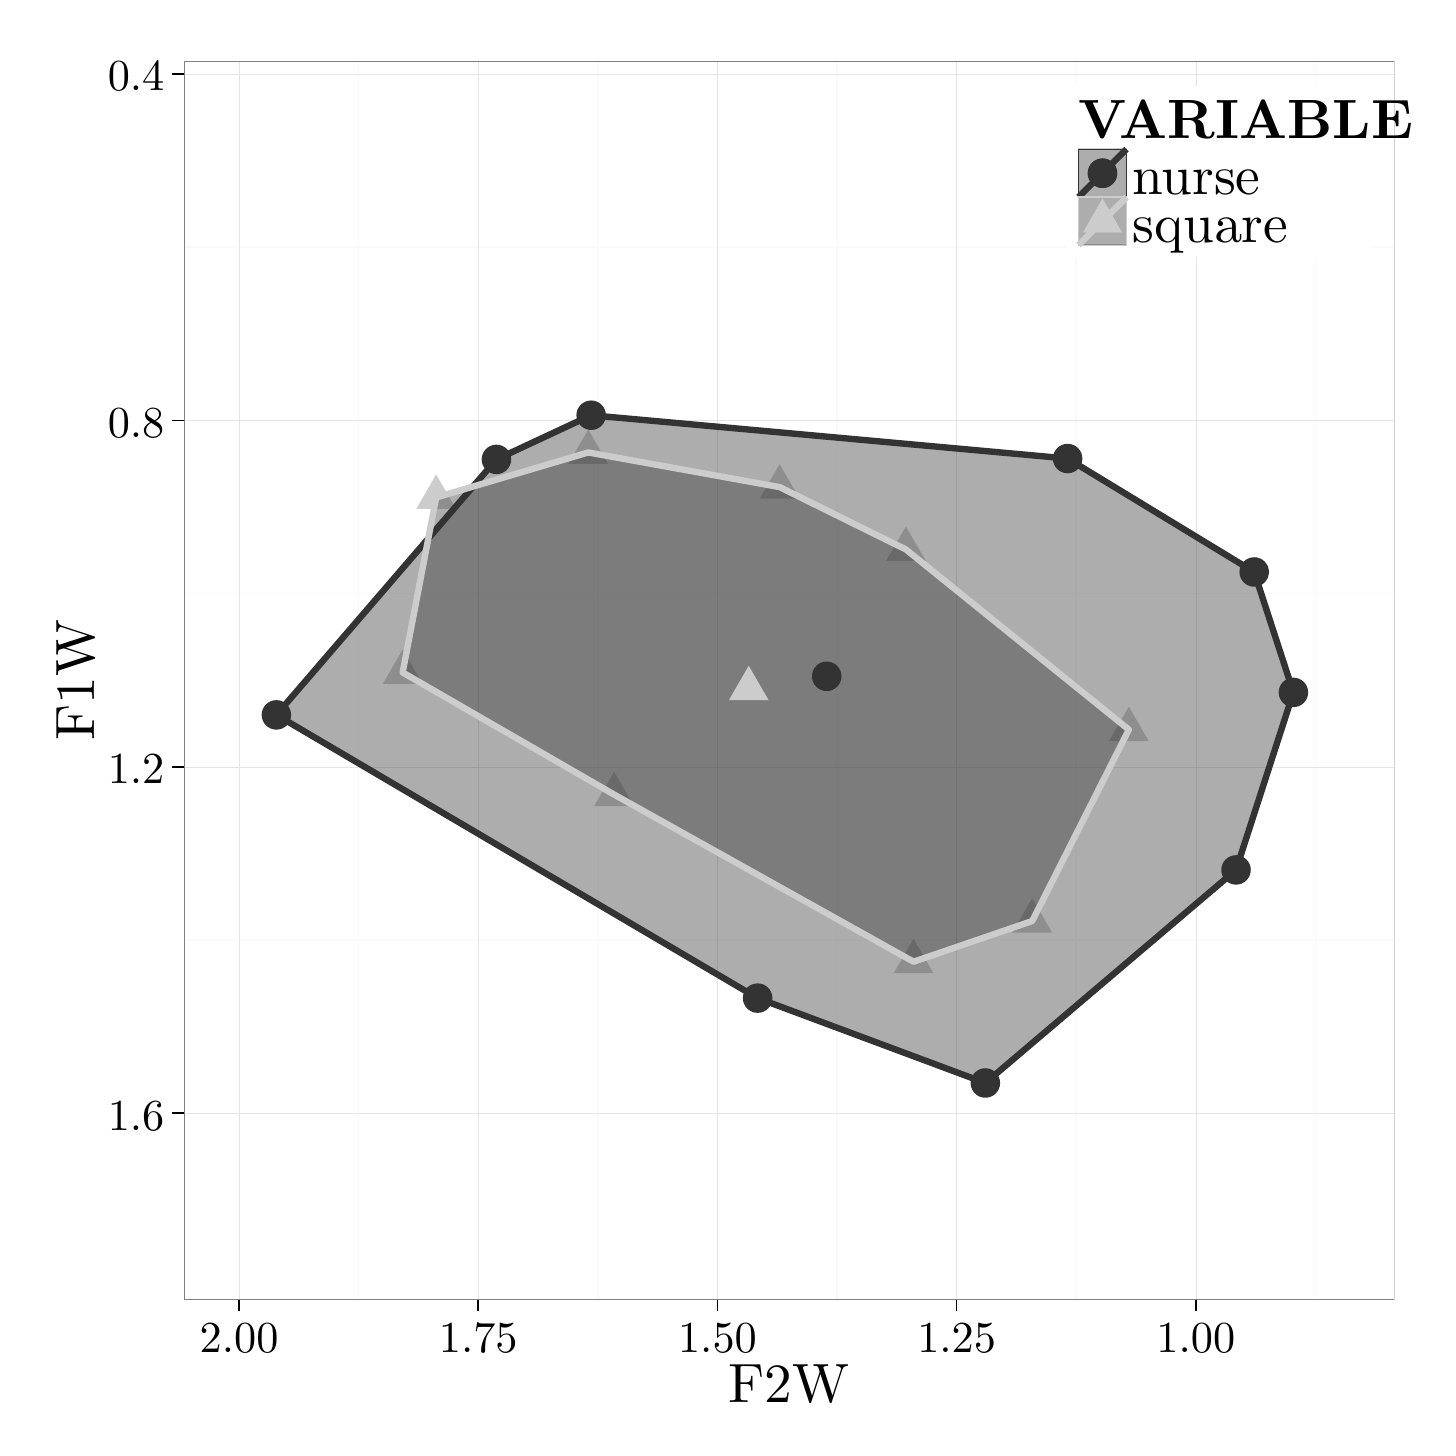
\begin{tikzpicture}[x=1pt,y=1pt]
\definecolor{fillColor}{RGB}{255,255,255}
\path[use as bounding box,fill=fillColor,fill opacity=0.00] (0,0) rectangle (505.89,505.89);
\begin{scope}
\path[clip] (  0.00,  0.00) rectangle (505.89,505.89);
\definecolor{drawColor}{RGB}{255,255,255}
\definecolor{fillColor}{RGB}{255,255,255}

\path[draw=drawColor,line width= 0.6pt,line join=round,line cap=round,fill=fillColor] (  0.00, -0.00) rectangle (505.89,505.89);
\end{scope}
\begin{scope}
\path[clip] ( 56.50, 46.31) rectangle (493.85,493.84);
\definecolor{fillColor}{RGB}{255,255,255}

\path[fill=fillColor] ( 56.50, 46.31) rectangle (493.85,493.84);
\definecolor{drawColor}{gray}{0.98}

\path[draw=drawColor,line width= 0.6pt,line join=round] ( 56.50,426.56) --
	(493.85,426.56);

\path[draw=drawColor,line width= 0.6pt,line join=round] ( 56.50,301.37) --
	(493.85,301.37);

\path[draw=drawColor,line width= 0.6pt,line join=round] ( 56.50,176.19) --
	(493.85,176.19);

\path[draw=drawColor,line width= 0.6pt,line join=round] (465.32, 46.31) --
	(465.32,493.84);

\path[draw=drawColor,line width= 0.6pt,line join=round] (378.89, 46.31) --
	(378.89,493.84);

\path[draw=drawColor,line width= 0.6pt,line join=round] (292.46, 46.31) --
	(292.46,493.84);

\path[draw=drawColor,line width= 0.6pt,line join=round] (206.03, 46.31) --
	(206.03,493.84);

\path[draw=drawColor,line width= 0.6pt,line join=round] (119.60, 46.31) --
	(119.60,493.84);
\definecolor{drawColor}{gray}{0.90}

\path[draw=drawColor,line width= 0.2pt,line join=round] ( 56.50,489.15) --
	(493.85,489.15);

\path[draw=drawColor,line width= 0.2pt,line join=round] ( 56.50,363.97) --
	(493.85,363.97);

\path[draw=drawColor,line width= 0.2pt,line join=round] ( 56.50,238.78) --
	(493.85,238.78);

\path[draw=drawColor,line width= 0.2pt,line join=round] ( 56.50,113.59) --
	(493.85,113.59);

\path[draw=drawColor,line width= 0.2pt,line join=round] (422.11, 46.31) --
	(422.11,493.84);

\path[draw=drawColor,line width= 0.2pt,line join=round] (335.68, 46.31) --
	(335.68,493.84);

\path[draw=drawColor,line width= 0.2pt,line join=round] (249.24, 46.31) --
	(249.24,493.84);

\path[draw=drawColor,line width= 0.2pt,line join=round] (162.81, 46.31) --
	(162.81,493.84);

\path[draw=drawColor,line width= 0.2pt,line join=round] ( 76.38, 46.31) --
	( 76.38,493.84);
\definecolor{fillColor}{gray}{0.20}

\path[fill=fillColor] (169.38,349.88) circle (  5.33);

\path[fill=fillColor] (203.61,365.84) circle (  5.33);

\path[fill=fillColor] (375.78,350.19) circle (  5.33);

\path[fill=fillColor] (443.20,309.20) circle (  5.33);

\path[fill=fillColor] (457.37,265.69) circle (  5.33);

\path[fill=fillColor] (436.63,201.54) circle (  5.33);

\path[fill=fillColor] (346.05,124.55) circle (  5.33);

\path[fill=fillColor] (263.77,155.22) circle (  5.33);

\path[fill=fillColor] ( 89.87,257.56) circle (  5.33);
\definecolor{fillColor}{gray}{0.80}

\path[fill=fillColor] (135.50,281.19) --
	(142.69,268.74) --
	(128.32,268.74) --
	cycle;

\path[fill=fillColor] (147.60,344.41) --
	(154.79,331.96) --
	(140.42,331.96) --
	cycle;

\path[fill=fillColor] (202.57,360.68) --
	(209.76,348.24) --
	(195.39,348.24) --
	cycle;

\path[fill=fillColor] (271.72,348.16) --
	(278.90,335.72) --
	(264.53,335.72) --
	cycle;

\path[fill=fillColor] (317.35,325.63) --
	(324.54,313.19) --
	(310.17,313.19) --
	cycle;

\path[fill=fillColor] (397.91,260.53) --
	(405.09,248.09) --
	(390.72,248.09) --
	cycle;

\path[fill=fillColor] (362.99,191.37) --
	(370.17,178.92) --
	(355.80,178.92) --
	cycle;

\path[fill=fillColor] (320.12,176.66) --
	(327.30,164.22) --
	(312.93,164.22) --
	cycle;

\path[fill=fillColor] (211.91,237.06) --
	(219.09,224.62) --
	(204.72,224.62) --
	cycle;
\definecolor{drawColor}{gray}{0.20}
\definecolor{fillColor}{RGB}{51,51,51}

\path[draw=drawColor,line width= 2.3pt,line join=round,line cap=round,fill=fillColor,fill opacity=0.40] (169.38,349.88) --
	(203.61,365.84) --
	(375.78,350.19) --
	(443.20,309.20) --
	(457.37,265.69) --
	(436.63,201.54) --
	(346.05,124.55) --
	(263.77,155.22) --
	( 89.87,257.56) --
	cycle;
\definecolor{drawColor}{gray}{0.80}

\path[draw=drawColor,line width= 2.3pt,line join=round,line cap=round,fill=fillColor,fill opacity=0.40] (135.50,272.89) --
	(147.60,336.11) --
	(202.57,352.39) --
	(271.72,339.87) --
	(317.35,317.33) --
	(397.91,252.24) --
	(362.99,183.07) --
	(320.12,168.36) --
	(211.91,228.77) --
	cycle;
\definecolor{fillColor}{gray}{0.20}

\path[fill=fillColor] (288.73,271.51) circle (  5.33);
\definecolor{fillColor}{gray}{0.80}

\path[fill=fillColor] (260.55,275.31) --
	(267.74,262.87) --
	(253.37,262.87) --
	cycle;
\definecolor{drawColor}{gray}{0.50}

\path[draw=drawColor,line width= 0.6pt,line join=round,line cap=round] ( 56.50, 46.31) rectangle (493.85,493.84);
\end{scope}
\begin{scope}
\path[clip] (  0.00,  0.00) rectangle (505.89,505.89);
\definecolor{drawColor}{RGB}{0,0,0}

\node[text=drawColor,anchor=base east,inner sep=0pt, outer sep=0pt, scale=  1.60] at ( 49.39,483.12) {0.4};

\node[text=drawColor,anchor=base east,inner sep=0pt, outer sep=0pt, scale=  1.60] at ( 49.39,357.93) {0.8};

\node[text=drawColor,anchor=base east,inner sep=0pt, outer sep=0pt, scale=  1.60] at ( 49.39,232.75) {1.2};

\node[text=drawColor,anchor=base east,inner sep=0pt, outer sep=0pt, scale=  1.60] at ( 49.39,107.56) {1.6};
\end{scope}
\begin{scope}
\path[clip] (  0.00,  0.00) rectangle (505.89,505.89);
\definecolor{drawColor}{RGB}{0,0,0}

\path[draw=drawColor,line width= 0.6pt,line join=round] ( 52.24,489.15) --
	( 56.50,489.15);

\path[draw=drawColor,line width= 0.6pt,line join=round] ( 52.24,363.97) --
	( 56.50,363.97);

\path[draw=drawColor,line width= 0.6pt,line join=round] ( 52.24,238.78) --
	( 56.50,238.78);

\path[draw=drawColor,line width= 0.6pt,line join=round] ( 52.24,113.59) --
	( 56.50,113.59);
\end{scope}
\begin{scope}
\path[clip] (  0.00,  0.00) rectangle (505.89,505.89);
\definecolor{drawColor}{RGB}{0,0,0}

\path[draw=drawColor,line width= 0.6pt,line join=round] (422.11, 42.04) --
	(422.11, 46.31);

\path[draw=drawColor,line width= 0.6pt,line join=round] (335.68, 42.04) --
	(335.68, 46.31);

\path[draw=drawColor,line width= 0.6pt,line join=round] (249.24, 42.04) --
	(249.24, 46.31);

\path[draw=drawColor,line width= 0.6pt,line join=round] (162.81, 42.04) --
	(162.81, 46.31);

\path[draw=drawColor,line width= 0.6pt,line join=round] ( 76.38, 42.04) --
	( 76.38, 46.31);
\end{scope}
\begin{scope}
\path[clip] (  0.00,  0.00) rectangle (505.89,505.89);
\definecolor{drawColor}{RGB}{0,0,0}

\node[text=drawColor,anchor=base,inner sep=0pt, outer sep=0pt, scale=  1.60] at (422.11, 27.13) {1.00};

\node[text=drawColor,anchor=base,inner sep=0pt, outer sep=0pt, scale=  1.60] at (335.68, 27.13) {1.25};

\node[text=drawColor,anchor=base,inner sep=0pt, outer sep=0pt, scale=  1.60] at (249.24, 27.13) {1.50};

\node[text=drawColor,anchor=base,inner sep=0pt, outer sep=0pt, scale=  1.60] at (162.81, 27.13) {1.75};

\node[text=drawColor,anchor=base,inner sep=0pt, outer sep=0pt, scale=  1.60] at ( 76.38, 27.13) {2.00};
\end{scope}
\begin{scope}
\path[clip] (  0.00,  0.00) rectangle (505.89,505.89);
\definecolor{drawColor}{RGB}{0,0,0}

\node[text=drawColor,anchor=base,inner sep=0pt, outer sep=0pt, scale=  2.00] at (275.17,  9.03) {F2W};
\end{scope}
\begin{scope}
\path[clip] (  0.00,  0.00) rectangle (505.89,505.89);
\definecolor{drawColor}{RGB}{0,0,0}

\node[text=drawColor,rotate= 90.00,anchor=base,inner sep=0pt, outer sep=0pt, scale=  2.00] at ( 24.12,270.08) {F1W};
\end{scope}
\begin{scope}
\path[clip] (  0.00,  0.00) rectangle (505.89,505.89);
\definecolor{fillColor}{RGB}{255,255,255}

\path[fill=fillColor] (375.44,423.00) rectangle (484.98,484.98);
\end{scope}
\begin{scope}
\path[clip] (  0.00,  0.00) rectangle (505.89,505.89);
\definecolor{drawColor}{RGB}{0,0,0}

\node[text=drawColor,anchor=base west,inner sep=0pt, outer sep=0pt, scale=  2.00] at (379.71,465.96) {\bfseries VARIABLE};
\end{scope}
\begin{scope}
\path[clip] (  0.00,  0.00) rectangle (505.89,505.89);
\definecolor{drawColor}{gray}{0.80}
\definecolor{fillColor}{RGB}{255,255,255}

\path[draw=drawColor,line width= 0.6pt,line join=round,line cap=round,fill=fillColor] (379.71,444.61) rectangle (397.06,461.96);
\end{scope}
\begin{scope}
\path[clip] (  0.00,  0.00) rectangle (505.89,505.89);
\definecolor{fillColor}{gray}{0.20}

\path[fill=fillColor] (388.38,453.29) circle (  5.33);
\end{scope}
\begin{scope}
\path[clip] (  0.00,  0.00) rectangle (505.89,505.89);
\definecolor{drawColor}{gray}{0.20}
\definecolor{fillColor}{RGB}{51,51,51}

\path[draw=drawColor,line width= 0.4pt,line join=round,line cap=round,fill=fillColor,fill opacity=0.40] (379.71,444.61) rectangle (397.06,461.96);

\path[draw=drawColor,line width= 2.3pt,line join=round] (379.71,444.61) --
	(397.06,461.96);
\end{scope}
\begin{scope}
\path[clip] (  0.00,  0.00) rectangle (505.89,505.89);
\definecolor{fillColor}{gray}{0.20}

\path[fill=fillColor] (388.38,453.29) circle (  5.33);
\end{scope}
\begin{scope}
\path[clip] (  0.00,  0.00) rectangle (505.89,505.89);
\definecolor{drawColor}{gray}{0.80}
\definecolor{fillColor}{RGB}{255,255,255}

\path[draw=drawColor,line width= 0.6pt,line join=round,line cap=round,fill=fillColor] (379.71,427.27) rectangle (397.06,444.61);
\end{scope}
\begin{scope}
\path[clip] (  0.00,  0.00) rectangle (505.89,505.89);
\definecolor{fillColor}{gray}{0.80}

\path[fill=fillColor] (388.38,444.24) --
	(395.57,431.79) --
	(381.20,431.79) --
	cycle;
\end{scope}
\begin{scope}
\path[clip] (  0.00,  0.00) rectangle (505.89,505.89);
\definecolor{drawColor}{gray}{0.80}
\definecolor{fillColor}{RGB}{51,51,51}

\path[draw=drawColor,line width= 0.4pt,line join=round,line cap=round,fill=fillColor,fill opacity=0.40] (379.71,427.27) rectangle (397.06,444.61);

\path[draw=drawColor,line width= 2.3pt,line join=round] (379.71,427.27) --
	(397.06,444.61);
\end{scope}
\begin{scope}
\path[clip] (  0.00,  0.00) rectangle (505.89,505.89);
\definecolor{fillColor}{gray}{0.80}

\path[fill=fillColor] (388.38,444.24) --
	(395.57,431.79) --
	(381.20,431.79) --
	cycle;
\end{scope}
\begin{scope}
\path[clip] (  0.00,  0.00) rectangle (505.89,505.89);
\definecolor{drawColor}{RGB}{0,0,0}

\node[text=drawColor,anchor=base west,inner sep=0pt, outer sep=0pt, scale=  2.00] at (399.22,445.75) {nurse};
\end{scope}
\begin{scope}
\path[clip] (  0.00,  0.00) rectangle (505.89,505.89);
\definecolor{drawColor}{RGB}{0,0,0}

\node[text=drawColor,anchor=base west,inner sep=0pt, outer sep=0pt, scale=  2.00] at (399.22,428.40) {square};
\end{scope}
\end{tikzpicture}
} 
		\caption{spontaneous speech}
		\label{fig.nurse.space.mid.free}
	\end{subfigure}
	\begin{subfigure}{.49\textwidth}
		\centering
			\definecolor{shadecolor}{rgb}{0.969, 0.969, 0.969}
			\resizebox{\linewidth}{!}{% Created by tikzDevice version 0.8.1 on 2016-02-09 02:15:25
% !TEX encoding = UTF-8 Unicode
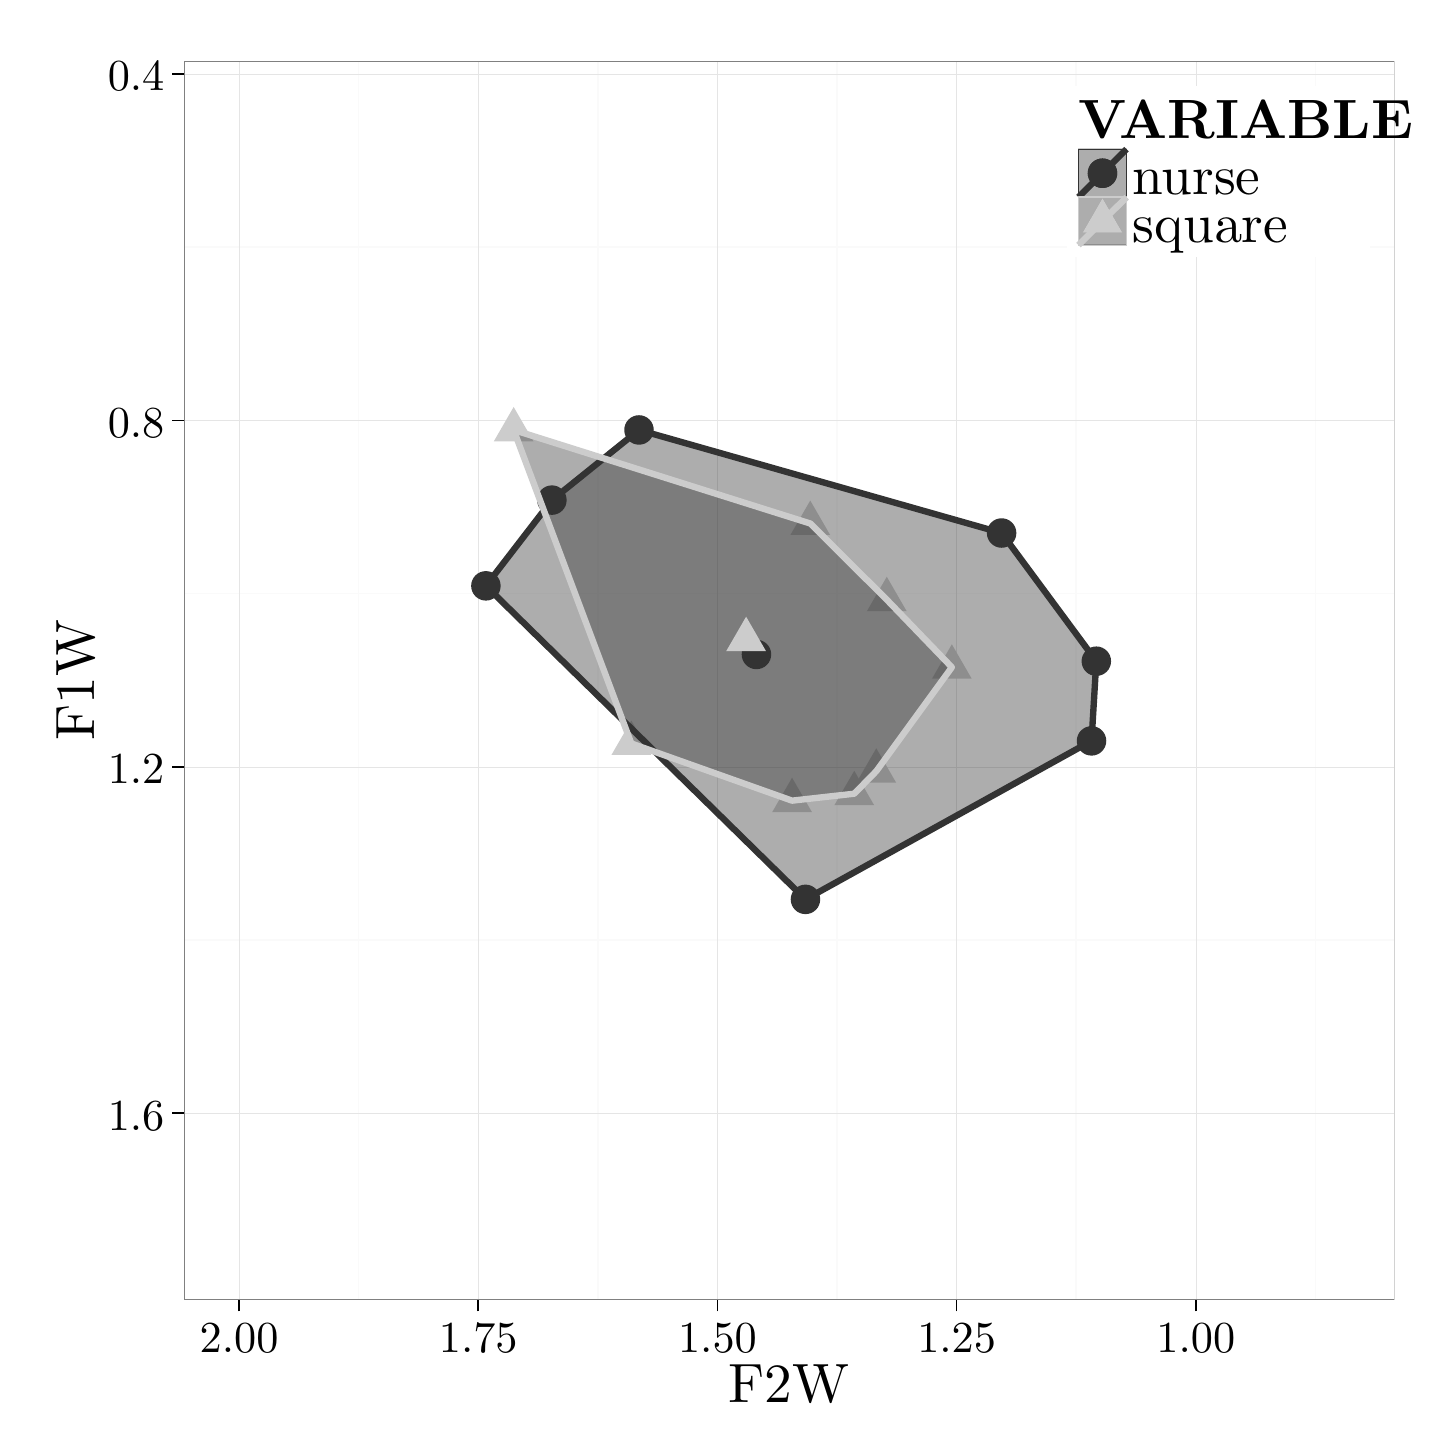
\begin{tikzpicture}[x=1pt,y=1pt]
\definecolor{fillColor}{RGB}{255,255,255}
\path[use as bounding box,fill=fillColor,fill opacity=0.00] (0,0) rectangle (505.89,505.89);
\begin{scope}
\path[clip] (  0.00,  0.00) rectangle (505.89,505.89);
\definecolor{drawColor}{RGB}{255,255,255}
\definecolor{fillColor}{RGB}{255,255,255}

\path[draw=drawColor,line width= 0.6pt,line join=round,line cap=round,fill=fillColor] (  0.00, -0.00) rectangle (505.89,505.89);
\end{scope}
\begin{scope}
\path[clip] ( 56.50, 46.31) rectangle (493.85,493.84);
\definecolor{fillColor}{RGB}{255,255,255}

\path[fill=fillColor] ( 56.50, 46.31) rectangle (493.85,493.84);
\definecolor{drawColor}{gray}{0.98}

\path[draw=drawColor,line width= 0.6pt,line join=round] ( 56.50,426.56) --
	(493.85,426.56);

\path[draw=drawColor,line width= 0.6pt,line join=round] ( 56.50,301.37) --
	(493.85,301.37);

\path[draw=drawColor,line width= 0.6pt,line join=round] ( 56.50,176.19) --
	(493.85,176.19);

\path[draw=drawColor,line width= 0.6pt,line join=round] (465.32, 46.31) --
	(465.32,493.84);

\path[draw=drawColor,line width= 0.6pt,line join=round] (378.89, 46.31) --
	(378.89,493.84);

\path[draw=drawColor,line width= 0.6pt,line join=round] (292.46, 46.31) --
	(292.46,493.84);

\path[draw=drawColor,line width= 0.6pt,line join=round] (206.03, 46.31) --
	(206.03,493.84);

\path[draw=drawColor,line width= 0.6pt,line join=round] (119.60, 46.31) --
	(119.60,493.84);
\definecolor{drawColor}{gray}{0.90}

\path[draw=drawColor,line width= 0.2pt,line join=round] ( 56.50,489.15) --
	(493.85,489.15);

\path[draw=drawColor,line width= 0.2pt,line join=round] ( 56.50,363.97) --
	(493.85,363.97);

\path[draw=drawColor,line width= 0.2pt,line join=round] ( 56.50,238.78) --
	(493.85,238.78);

\path[draw=drawColor,line width= 0.2pt,line join=round] ( 56.50,113.59) --
	(493.85,113.59);

\path[draw=drawColor,line width= 0.2pt,line join=round] (422.11, 46.31) --
	(422.11,493.84);

\path[draw=drawColor,line width= 0.2pt,line join=round] (335.68, 46.31) --
	(335.68,493.84);

\path[draw=drawColor,line width= 0.2pt,line join=round] (249.24, 46.31) --
	(249.24,493.84);

\path[draw=drawColor,line width= 0.2pt,line join=round] (162.81, 46.31) --
	(162.81,493.84);

\path[draw=drawColor,line width= 0.2pt,line join=round] ( 76.38, 46.31) --
	( 76.38,493.84);
\definecolor{fillColor}{gray}{0.20}

\path[fill=fillColor] (165.58,304.19) circle (  5.33);

\path[fill=fillColor] (189.43,335.17) circle (  5.33);

\path[fill=fillColor] (220.90,360.52) circle (  5.33);

\path[fill=fillColor] (351.93,323.28) circle (  5.33);

\path[fill=fillColor] (386.15,276.96) circle (  5.33);

\path[fill=fillColor] (384.42,248.17) circle (  5.33);

\path[fill=fillColor] (281.05,190.90) circle (  5.33);
\definecolor{fillColor}{gray}{0.80}

\path[fill=fillColor] (175.61,368.82) --
	(182.79,356.37) --
	(168.42,356.37) --
	cycle;

\path[fill=fillColor] (282.78,335.02) --
	(289.97,322.57) --
	(275.60,322.57) --
	cycle;

\path[fill=fillColor] (310.44,307.48) --
	(317.62,295.03) --
	(303.25,295.03) --
	cycle;

\path[fill=fillColor] (333.95,283.07) --
	(341.13,270.62) --
	(326.76,270.62) --
	cycle;

\path[fill=fillColor] (306.64,245.51) --
	(313.82,233.07) --
	(299.45,233.07) --
	cycle;

\path[fill=fillColor] (298.68,237.37) --
	(305.87,224.93) --
	(291.50,224.93) --
	cycle;

\path[fill=fillColor] (276.21,234.87) --
	(283.40,222.43) --
	(269.03,222.43) --
	cycle;

\path[fill=fillColor] (218.13,255.53) --
	(225.31,243.08) --
	(210.94,243.08) --
	cycle;
\definecolor{drawColor}{gray}{0.20}
\definecolor{fillColor}{RGB}{51,51,51}

\path[draw=drawColor,line width= 2.3pt,line join=round,line cap=round,fill=fillColor,fill opacity=0.40] (165.58,304.19) --
	(189.43,335.17) --
	(220.90,360.52) --
	(351.93,323.28) --
	(386.15,276.96) --
	(384.42,248.17) --
	(281.05,190.90) --
	cycle;
\definecolor{drawColor}{gray}{0.80}

\path[draw=drawColor,line width= 2.3pt,line join=round,line cap=round,fill=fillColor,fill opacity=0.40] (175.61,360.52) --
	(282.78,326.72) --
	(310.44,299.18) --
	(333.95,274.77) --
	(306.64,237.22) --
	(298.68,229.08) --
	(276.21,226.57) --
	(218.13,247.23) --
	cycle;
\definecolor{fillColor}{gray}{0.20}

\path[fill=fillColor] (263.34,279.40) circle (  5.33);
\definecolor{fillColor}{gray}{0.80}

\path[fill=fillColor] (259.61,293.05) --
	(266.79,280.60) --
	(252.42,280.60) --
	cycle;
\definecolor{drawColor}{gray}{0.50}

\path[draw=drawColor,line width= 0.6pt,line join=round,line cap=round] ( 56.50, 46.31) rectangle (493.85,493.84);
\end{scope}
\begin{scope}
\path[clip] (  0.00,  0.00) rectangle (505.89,505.89);
\definecolor{drawColor}{RGB}{0,0,0}

\node[text=drawColor,anchor=base east,inner sep=0pt, outer sep=0pt, scale=  1.60] at ( 49.39,483.12) {0.4};

\node[text=drawColor,anchor=base east,inner sep=0pt, outer sep=0pt, scale=  1.60] at ( 49.39,357.93) {0.8};

\node[text=drawColor,anchor=base east,inner sep=0pt, outer sep=0pt, scale=  1.60] at ( 49.39,232.75) {1.2};

\node[text=drawColor,anchor=base east,inner sep=0pt, outer sep=0pt, scale=  1.60] at ( 49.39,107.56) {1.6};
\end{scope}
\begin{scope}
\path[clip] (  0.00,  0.00) rectangle (505.89,505.89);
\definecolor{drawColor}{RGB}{0,0,0}

\path[draw=drawColor,line width= 0.6pt,line join=round] ( 52.24,489.15) --
	( 56.50,489.15);

\path[draw=drawColor,line width= 0.6pt,line join=round] ( 52.24,363.97) --
	( 56.50,363.97);

\path[draw=drawColor,line width= 0.6pt,line join=round] ( 52.24,238.78) --
	( 56.50,238.78);

\path[draw=drawColor,line width= 0.6pt,line join=round] ( 52.24,113.59) --
	( 56.50,113.59);
\end{scope}
\begin{scope}
\path[clip] (  0.00,  0.00) rectangle (505.89,505.89);
\definecolor{drawColor}{RGB}{0,0,0}

\path[draw=drawColor,line width= 0.6pt,line join=round] (422.11, 42.04) --
	(422.11, 46.31);

\path[draw=drawColor,line width= 0.6pt,line join=round] (335.68, 42.04) --
	(335.68, 46.31);

\path[draw=drawColor,line width= 0.6pt,line join=round] (249.24, 42.04) --
	(249.24, 46.31);

\path[draw=drawColor,line width= 0.6pt,line join=round] (162.81, 42.04) --
	(162.81, 46.31);

\path[draw=drawColor,line width= 0.6pt,line join=round] ( 76.38, 42.04) --
	( 76.38, 46.31);
\end{scope}
\begin{scope}
\path[clip] (  0.00,  0.00) rectangle (505.89,505.89);
\definecolor{drawColor}{RGB}{0,0,0}

\node[text=drawColor,anchor=base,inner sep=0pt, outer sep=0pt, scale=  1.60] at (422.11, 27.13) {1.00};

\node[text=drawColor,anchor=base,inner sep=0pt, outer sep=0pt, scale=  1.60] at (335.68, 27.13) {1.25};

\node[text=drawColor,anchor=base,inner sep=0pt, outer sep=0pt, scale=  1.60] at (249.24, 27.13) {1.50};

\node[text=drawColor,anchor=base,inner sep=0pt, outer sep=0pt, scale=  1.60] at (162.81, 27.13) {1.75};

\node[text=drawColor,anchor=base,inner sep=0pt, outer sep=0pt, scale=  1.60] at ( 76.38, 27.13) {2.00};
\end{scope}
\begin{scope}
\path[clip] (  0.00,  0.00) rectangle (505.89,505.89);
\definecolor{drawColor}{RGB}{0,0,0}

\node[text=drawColor,anchor=base,inner sep=0pt, outer sep=0pt, scale=  2.00] at (275.17,  9.03) {F2W};
\end{scope}
\begin{scope}
\path[clip] (  0.00,  0.00) rectangle (505.89,505.89);
\definecolor{drawColor}{RGB}{0,0,0}

\node[text=drawColor,rotate= 90.00,anchor=base,inner sep=0pt, outer sep=0pt, scale=  2.00] at ( 24.12,270.08) {F1W};
\end{scope}
\begin{scope}
\path[clip] (  0.00,  0.00) rectangle (505.89,505.89);
\definecolor{fillColor}{RGB}{255,255,255}

\path[fill=fillColor] (375.44,423.00) rectangle (484.98,484.98);
\end{scope}
\begin{scope}
\path[clip] (  0.00,  0.00) rectangle (505.89,505.89);
\definecolor{drawColor}{RGB}{0,0,0}

\node[text=drawColor,anchor=base west,inner sep=0pt, outer sep=0pt, scale=  2.00] at (379.71,465.96) {\bfseries VARIABLE};
\end{scope}
\begin{scope}
\path[clip] (  0.00,  0.00) rectangle (505.89,505.89);
\definecolor{drawColor}{gray}{0.80}
\definecolor{fillColor}{RGB}{255,255,255}

\path[draw=drawColor,line width= 0.6pt,line join=round,line cap=round,fill=fillColor] (379.71,444.61) rectangle (397.06,461.96);
\end{scope}
\begin{scope}
\path[clip] (  0.00,  0.00) rectangle (505.89,505.89);
\definecolor{fillColor}{gray}{0.20}

\path[fill=fillColor] (388.38,453.29) circle (  5.33);
\end{scope}
\begin{scope}
\path[clip] (  0.00,  0.00) rectangle (505.89,505.89);
\definecolor{drawColor}{gray}{0.20}
\definecolor{fillColor}{RGB}{51,51,51}

\path[draw=drawColor,line width= 0.4pt,line join=round,line cap=round,fill=fillColor,fill opacity=0.40] (379.71,444.61) rectangle (397.06,461.96);

\path[draw=drawColor,line width= 2.3pt,line join=round] (379.71,444.61) --
	(397.06,461.96);
\end{scope}
\begin{scope}
\path[clip] (  0.00,  0.00) rectangle (505.89,505.89);
\definecolor{fillColor}{gray}{0.20}

\path[fill=fillColor] (388.38,453.29) circle (  5.33);
\end{scope}
\begin{scope}
\path[clip] (  0.00,  0.00) rectangle (505.89,505.89);
\definecolor{drawColor}{gray}{0.80}
\definecolor{fillColor}{RGB}{255,255,255}

\path[draw=drawColor,line width= 0.6pt,line join=round,line cap=round,fill=fillColor] (379.71,427.27) rectangle (397.06,444.61);
\end{scope}
\begin{scope}
\path[clip] (  0.00,  0.00) rectangle (505.89,505.89);
\definecolor{fillColor}{gray}{0.80}

\path[fill=fillColor] (388.38,444.24) --
	(395.57,431.79) --
	(381.20,431.79) --
	cycle;
\end{scope}
\begin{scope}
\path[clip] (  0.00,  0.00) rectangle (505.89,505.89);
\definecolor{drawColor}{gray}{0.80}
\definecolor{fillColor}{RGB}{51,51,51}

\path[draw=drawColor,line width= 0.4pt,line join=round,line cap=round,fill=fillColor,fill opacity=0.40] (379.71,427.27) rectangle (397.06,444.61);

\path[draw=drawColor,line width= 2.3pt,line join=round] (379.71,427.27) --
	(397.06,444.61);
\end{scope}
\begin{scope}
\path[clip] (  0.00,  0.00) rectangle (505.89,505.89);
\definecolor{fillColor}{gray}{0.80}

\path[fill=fillColor] (388.38,444.24) --
	(395.57,431.79) --
	(381.20,431.79) --
	cycle;
\end{scope}
\begin{scope}
\path[clip] (  0.00,  0.00) rectangle (505.89,505.89);
\definecolor{drawColor}{RGB}{0,0,0}

\node[text=drawColor,anchor=base west,inner sep=0pt, outer sep=0pt, scale=  2.00] at (399.22,445.75) {nurse};
\end{scope}
\begin{scope}
\path[clip] (  0.00,  0.00) rectangle (505.89,505.89);
\definecolor{drawColor}{RGB}{0,0,0}

\node[text=drawColor,anchor=base west,inner sep=0pt, outer sep=0pt, scale=  2.00] at (399.22,428.40) {square};
\end{scope}
\end{tikzpicture}
} 
		\caption{accent performance}
		\label{fig.nurse.space.mid.imit}
	\end{subfigure}
	
	\caption{\textsc{nurse}-\textsc{square}: vowel space by style (middle-aged speakers)}
	\label{fig.nurse.space.mid}
\end{figure}

When we turn to the data collected in the group of middle-aged speakers (Figure \ref{fig.nurse.space.mid}) and compare them to \textsc{nurse} and \textsc{square} realisations of the old group, both similarities and differences emerge.
For instance, \textsc{nurse} is again always more variable than \textsc{square}, which is expected since \textsc{square} is supposed to be the steady target of the merger.
Just as in the old group, there is also clearly more variation (for both vowels) in spontaneous speech than in the other speaking styles.
But in contrast to the older generation, the lowest degree of variation is found for accent imitation\is{accent performance}, while the word list and reading passage seem to be roughly comparable in this respect.
However, it should be noted that the realisational spaces --- particularly when comparing the word list, reading, and accent perform\is{accent performance}ance --- differ less in area in the middle-aged group, generally, which is to say that the range of variation depends less on style than in the old group.
All the same, it looks as if, again, the target realisations for the more formal and the \isi{stereotype} contexts are clearer, or less controversial, than in spontaneous speech, where a wider range of phonetic variants is encountered.
The most pronounced difference between the old and the middle-aged speakers is that in the former most variation is found in the height dimension, whereas in the latter group the horizontal extent of the individual vowel spaces is at least as great as, and frequently greater than, the vertical one, which means that the main axis of variation seems to be F2 in this age group.

With respect to the centres of gravity of these vowel clouds, there is something going on that is even more interesting than the pattern found for the older speakers.
In spontaneous speech (Figure \ref{fig.nurse.space.mid.free}), the relative positioning of \textsc{nurse} and \textsc{square} is identical to the one found for the older speakers: \textsc{nurse} is both slightly higher and backer than \textsc{square}, which corresponds to the setup expected on the basis of the standard if the vowels are not perfectly merged yet.
The means of the two distributions are also further apart from each other than in the other styles, although the difference is smaller than in the old speakers.
If this register is once again taken as the benchmark, or baseline, both \textsc{nurse} and \textsc{square} change when people are asked to put on a particularly strong Scouse accent (Figure \ref{fig.nurse.space.mid.imit}): The former is fronted, the latter slightly raised.
As a result, mean realisations of both vowels are essentially identical.
When we go the other way from less formal free speech to more formal reading (Figure \ref{fig.nurse.space.mid.read}), however, mean \textsc{nurse} remains almost the same, if one ignores the tiny amount of fronting that is visible.
In this register it is mostly \textsc{square} that moves: raising takes it closer to \textsc{nurse}.
This results in more \emph{merged} distributions (cf. Table \ref{tab.pillai.nurse.agestyle}), instead of the more \emph{distinct\is{distinctness}} ones that would normally be expected in a more formal speaking style.
When subjects read out a word list (Figure \ref{fig.nurse.space.mid.list}) \textsc{square} is centralised, while \textsc{nurse} is fronted at the same time.
The outcome of these processes is that \textsc{nurse} (dark circle) actually ends up in a position that is \emph{more front} than that of \textsc{square} (light triangle), thereby completely reversing the relative positioning found in spontaneous speech, at least with respect to the F2 dimension.

\subsubsection{Young speakers}

\begin{figure}[h!]
	\centering
	\begin{subfigure}{.49\textwidth}
		\centering
			\definecolor{shadecolor}{rgb}{0.969, 0.969, 0.969}
			\resizebox{\linewidth}{!}{% Created by tikzDevice version 0.8.1 on 2016-02-09 02:15:26
% !TEX encoding = UTF-8 Unicode
\begin{tikzpicture}[x=1pt,y=1pt]
\definecolor{fillColor}{RGB}{255,255,255}
\path[use as bounding box,fill=fillColor,fill opacity=0.00] (0,0) rectangle (505.89,505.89);
\begin{scope}
\path[clip] (  0.00,  0.00) rectangle (505.89,505.89);
\definecolor{drawColor}{RGB}{255,255,255}
\definecolor{fillColor}{RGB}{255,255,255}

\path[draw=drawColor,line width= 0.6pt,line join=round,line cap=round,fill=fillColor] (  0.00, -0.00) rectangle (505.89,505.89);
\end{scope}
\begin{scope}
\path[clip] ( 56.50, 46.31) rectangle (493.85,493.84);
\definecolor{fillColor}{RGB}{255,255,255}

\path[fill=fillColor] ( 56.50, 46.31) rectangle (493.85,493.84);
\definecolor{drawColor}{gray}{0.98}

\path[draw=drawColor,line width= 0.6pt,line join=round] ( 56.50,426.56) --
	(493.85,426.56);

\path[draw=drawColor,line width= 0.6pt,line join=round] ( 56.50,301.37) --
	(493.85,301.37);

\path[draw=drawColor,line width= 0.6pt,line join=round] ( 56.50,176.19) --
	(493.85,176.19);

\path[draw=drawColor,line width= 0.6pt,line join=round] (465.32, 46.31) --
	(465.32,493.84);

\path[draw=drawColor,line width= 0.6pt,line join=round] (378.89, 46.31) --
	(378.89,493.84);

\path[draw=drawColor,line width= 0.6pt,line join=round] (292.46, 46.31) --
	(292.46,493.84);

\path[draw=drawColor,line width= 0.6pt,line join=round] (206.03, 46.31) --
	(206.03,493.84);

\path[draw=drawColor,line width= 0.6pt,line join=round] (119.60, 46.31) --
	(119.60,493.84);
\definecolor{drawColor}{gray}{0.90}

\path[draw=drawColor,line width= 0.2pt,line join=round] ( 56.50,489.15) --
	(493.85,489.15);

\path[draw=drawColor,line width= 0.2pt,line join=round] ( 56.50,363.97) --
	(493.85,363.97);

\path[draw=drawColor,line width= 0.2pt,line join=round] ( 56.50,238.78) --
	(493.85,238.78);

\path[draw=drawColor,line width= 0.2pt,line join=round] ( 56.50,113.59) --
	(493.85,113.59);

\path[draw=drawColor,line width= 0.2pt,line join=round] (422.11, 46.31) --
	(422.11,493.84);

\path[draw=drawColor,line width= 0.2pt,line join=round] (335.68, 46.31) --
	(335.68,493.84);

\path[draw=drawColor,line width= 0.2pt,line join=round] (249.24, 46.31) --
	(249.24,493.84);

\path[draw=drawColor,line width= 0.2pt,line join=round] (162.81, 46.31) --
	(162.81,493.84);

\path[draw=drawColor,line width= 0.2pt,line join=round] ( 76.38, 46.31) --
	( 76.38,493.84);
\definecolor{fillColor}{gray}{0.20}

\path[fill=fillColor] (166.62,289.79) circle (  5.33);

\path[fill=fillColor] (183.90,303.25) circle (  5.33);

\path[fill=fillColor] (204.65,316.08) circle (  5.33);

\path[fill=fillColor] (266.53,319.84) circle (  5.33);

\path[fill=fillColor] (357.46,234.71) circle (  5.33);

\path[fill=fillColor] (313.20,179.63) circle (  5.33);

\path[fill=fillColor] (218.82,205.61) circle (  5.33);
\definecolor{fillColor}{gray}{0.80}

\path[fill=fillColor] (165.58,294.65) --
	(172.76,282.20) --
	(158.39,282.20) --
	cycle;

\path[fill=fillColor] (224.70,334.39) --
	(231.88,321.95) --
	(217.51,321.95) --
	cycle;

\path[fill=fillColor] (256.51,340.03) --
	(263.69,327.58) --
	(249.32,327.58) --
	cycle;

\path[fill=fillColor] (273.79,333.14) --
	(280.98,320.70) --
	(266.61,320.70) --
	cycle;

\path[fill=fillColor] (299.38,311.23) --
	(306.56,298.79) --
	(292.19,298.79) --
	cycle;

\path[fill=fillColor] (309.40,287.14) --
	(316.59,274.69) --
	(302.22,274.69) --
	cycle;

\path[fill=fillColor] (329.80,221.10) --
	(336.98,208.66) --
	(322.61,208.66) --
	cycle;

\path[fill=fillColor] (310.78,205.77) --
	(317.97,193.32) --
	(303.60,193.32) --
	cycle;

\path[fill=fillColor] (300.41,211.09) --
	(307.60,198.64) --
	(293.23,198.64) --
	cycle;

\path[fill=fillColor] (203.96,265.23) --
	(211.14,252.78) --
	(196.77,252.78) --
	cycle;
\definecolor{drawColor}{gray}{0.20}
\definecolor{fillColor}{RGB}{51,51,51}

\path[draw=drawColor,line width= 2.3pt,line join=round,line cap=round,fill=fillColor,fill opacity=0.40] (166.62,289.79) --
	(183.90,303.25) --
	(204.65,316.08) --
	(266.53,319.84) --
	(357.46,234.71) --
	(313.20,179.63) --
	(218.82,205.61) --
	cycle;
\definecolor{drawColor}{gray}{0.80}

\path[draw=drawColor,line width= 2.3pt,line join=round,line cap=round,fill=fillColor,fill opacity=0.40] (165.58,286.35) --
	(224.70,326.10) --
	(256.51,331.73) --
	(273.79,324.84) --
	(299.38,302.94) --
	(309.40,278.84) --
	(329.80,212.80) --
	(310.78,197.47) --
	(300.41,202.79) --
	(203.96,256.93) --
	cycle;
\definecolor{fillColor}{gray}{0.20}

\path[fill=fillColor] (256.42,267.37) circle (  5.33);
\definecolor{fillColor}{gray}{0.80}

\path[fill=fillColor] (261.10,281.42) --
	(268.29,268.98) --
	(253.92,268.98) --
	cycle;
\definecolor{drawColor}{gray}{0.50}

\path[draw=drawColor,line width= 0.6pt,line join=round,line cap=round] ( 56.50, 46.31) rectangle (493.85,493.84);
\end{scope}
\begin{scope}
\path[clip] (  0.00,  0.00) rectangle (505.89,505.89);
\definecolor{drawColor}{RGB}{0,0,0}

\node[text=drawColor,anchor=base east,inner sep=0pt, outer sep=0pt, scale=  1.60] at ( 49.39,483.12) {0.4};

\node[text=drawColor,anchor=base east,inner sep=0pt, outer sep=0pt, scale=  1.60] at ( 49.39,357.93) {0.8};

\node[text=drawColor,anchor=base east,inner sep=0pt, outer sep=0pt, scale=  1.60] at ( 49.39,232.75) {1.2};

\node[text=drawColor,anchor=base east,inner sep=0pt, outer sep=0pt, scale=  1.60] at ( 49.39,107.56) {1.6};
\end{scope}
\begin{scope}
\path[clip] (  0.00,  0.00) rectangle (505.89,505.89);
\definecolor{drawColor}{RGB}{0,0,0}

\path[draw=drawColor,line width= 0.6pt,line join=round] ( 52.24,489.15) --
	( 56.50,489.15);

\path[draw=drawColor,line width= 0.6pt,line join=round] ( 52.24,363.97) --
	( 56.50,363.97);

\path[draw=drawColor,line width= 0.6pt,line join=round] ( 52.24,238.78) --
	( 56.50,238.78);

\path[draw=drawColor,line width= 0.6pt,line join=round] ( 52.24,113.59) --
	( 56.50,113.59);
\end{scope}
\begin{scope}
\path[clip] (  0.00,  0.00) rectangle (505.89,505.89);
\definecolor{drawColor}{RGB}{0,0,0}

\path[draw=drawColor,line width= 0.6pt,line join=round] (422.11, 42.04) --
	(422.11, 46.31);

\path[draw=drawColor,line width= 0.6pt,line join=round] (335.68, 42.04) --
	(335.68, 46.31);

\path[draw=drawColor,line width= 0.6pt,line join=round] (249.24, 42.04) --
	(249.24, 46.31);

\path[draw=drawColor,line width= 0.6pt,line join=round] (162.81, 42.04) --
	(162.81, 46.31);

\path[draw=drawColor,line width= 0.6pt,line join=round] ( 76.38, 42.04) --
	( 76.38, 46.31);
\end{scope}
\begin{scope}
\path[clip] (  0.00,  0.00) rectangle (505.89,505.89);
\definecolor{drawColor}{RGB}{0,0,0}

\node[text=drawColor,anchor=base,inner sep=0pt, outer sep=0pt, scale=  1.60] at (422.11, 27.13) {1.00};

\node[text=drawColor,anchor=base,inner sep=0pt, outer sep=0pt, scale=  1.60] at (335.68, 27.13) {1.25};

\node[text=drawColor,anchor=base,inner sep=0pt, outer sep=0pt, scale=  1.60] at (249.24, 27.13) {1.50};

\node[text=drawColor,anchor=base,inner sep=0pt, outer sep=0pt, scale=  1.60] at (162.81, 27.13) {1.75};

\node[text=drawColor,anchor=base,inner sep=0pt, outer sep=0pt, scale=  1.60] at ( 76.38, 27.13) {2.00};
\end{scope}
\begin{scope}
\path[clip] (  0.00,  0.00) rectangle (505.89,505.89);
\definecolor{drawColor}{RGB}{0,0,0}

\node[text=drawColor,anchor=base,inner sep=0pt, outer sep=0pt, scale=  2.00] at (275.17,  9.03) {F2W};
\end{scope}
\begin{scope}
\path[clip] (  0.00,  0.00) rectangle (505.89,505.89);
\definecolor{drawColor}{RGB}{0,0,0}

\node[text=drawColor,rotate= 90.00,anchor=base,inner sep=0pt, outer sep=0pt, scale=  2.00] at ( 24.12,270.08) {F1W};
\end{scope}
\begin{scope}
\path[clip] (  0.00,  0.00) rectangle (505.89,505.89);
\definecolor{fillColor}{RGB}{255,255,255}

\path[fill=fillColor] (375.44,423.00) rectangle (484.98,484.98);
\end{scope}
\begin{scope}
\path[clip] (  0.00,  0.00) rectangle (505.89,505.89);
\definecolor{drawColor}{RGB}{0,0,0}

\node[text=drawColor,anchor=base west,inner sep=0pt, outer sep=0pt, scale=  2.00] at (379.71,465.96) {\bfseries VARIABLE};
\end{scope}
\begin{scope}
\path[clip] (  0.00,  0.00) rectangle (505.89,505.89);
\definecolor{drawColor}{gray}{0.80}
\definecolor{fillColor}{RGB}{255,255,255}

\path[draw=drawColor,line width= 0.6pt,line join=round,line cap=round,fill=fillColor] (379.71,444.61) rectangle (397.06,461.96);
\end{scope}
\begin{scope}
\path[clip] (  0.00,  0.00) rectangle (505.89,505.89);
\definecolor{fillColor}{gray}{0.20}

\path[fill=fillColor] (388.38,453.29) circle (  5.33);
\end{scope}
\begin{scope}
\path[clip] (  0.00,  0.00) rectangle (505.89,505.89);
\definecolor{drawColor}{gray}{0.20}
\definecolor{fillColor}{RGB}{51,51,51}

\path[draw=drawColor,line width= 0.4pt,line join=round,line cap=round,fill=fillColor,fill opacity=0.40] (379.71,444.61) rectangle (397.06,461.96);

\path[draw=drawColor,line width= 2.3pt,line join=round] (379.71,444.61) --
	(397.06,461.96);
\end{scope}
\begin{scope}
\path[clip] (  0.00,  0.00) rectangle (505.89,505.89);
\definecolor{fillColor}{gray}{0.20}

\path[fill=fillColor] (388.38,453.29) circle (  5.33);
\end{scope}
\begin{scope}
\path[clip] (  0.00,  0.00) rectangle (505.89,505.89);
\definecolor{drawColor}{gray}{0.80}
\definecolor{fillColor}{RGB}{255,255,255}

\path[draw=drawColor,line width= 0.6pt,line join=round,line cap=round,fill=fillColor] (379.71,427.27) rectangle (397.06,444.61);
\end{scope}
\begin{scope}
\path[clip] (  0.00,  0.00) rectangle (505.89,505.89);
\definecolor{fillColor}{gray}{0.80}

\path[fill=fillColor] (388.38,444.24) --
	(395.57,431.79) --
	(381.20,431.79) --
	cycle;
\end{scope}
\begin{scope}
\path[clip] (  0.00,  0.00) rectangle (505.89,505.89);
\definecolor{drawColor}{gray}{0.80}
\definecolor{fillColor}{RGB}{51,51,51}

\path[draw=drawColor,line width= 0.4pt,line join=round,line cap=round,fill=fillColor,fill opacity=0.40] (379.71,427.27) rectangle (397.06,444.61);

\path[draw=drawColor,line width= 2.3pt,line join=round] (379.71,427.27) --
	(397.06,444.61);
\end{scope}
\begin{scope}
\path[clip] (  0.00,  0.00) rectangle (505.89,505.89);
\definecolor{fillColor}{gray}{0.80}

\path[fill=fillColor] (388.38,444.24) --
	(395.57,431.79) --
	(381.20,431.79) --
	cycle;
\end{scope}
\begin{scope}
\path[clip] (  0.00,  0.00) rectangle (505.89,505.89);
\definecolor{drawColor}{RGB}{0,0,0}

\node[text=drawColor,anchor=base west,inner sep=0pt, outer sep=0pt, scale=  2.00] at (399.22,445.75) {nurse};
\end{scope}
\begin{scope}
\path[clip] (  0.00,  0.00) rectangle (505.89,505.89);
\definecolor{drawColor}{RGB}{0,0,0}

\node[text=drawColor,anchor=base west,inner sep=0pt, outer sep=0pt, scale=  2.00] at (399.22,428.40) {square};
\end{scope}
\end{tikzpicture}
} 
		\caption{word list}
		\label{fig.nurse.space.young.list}
	\end{subfigure}
	\begin{subfigure}{.49\textwidth}
		\centering
			\definecolor{shadecolor}{rgb}{0.969, 0.969, 0.969}
			\resizebox{\linewidth}{!}{% Created by tikzDevice version 0.8.1 on 2016-02-09 02:15:27
% !TEX encoding = UTF-8 Unicode
\begin{tikzpicture}[x=1pt,y=1pt]
\definecolor{fillColor}{RGB}{255,255,255}
\path[use as bounding box,fill=fillColor,fill opacity=0.00] (0,0) rectangle (505.89,505.89);
\begin{scope}
\path[clip] (  0.00,  0.00) rectangle (505.89,505.89);
\definecolor{drawColor}{RGB}{255,255,255}
\definecolor{fillColor}{RGB}{255,255,255}

\path[draw=drawColor,line width= 0.6pt,line join=round,line cap=round,fill=fillColor] (  0.00, -0.00) rectangle (505.89,505.89);
\end{scope}
\begin{scope}
\path[clip] ( 56.50, 46.31) rectangle (493.85,493.84);
\definecolor{fillColor}{RGB}{255,255,255}

\path[fill=fillColor] ( 56.50, 46.31) rectangle (493.85,493.84);
\definecolor{drawColor}{gray}{0.98}

\path[draw=drawColor,line width= 0.6pt,line join=round] ( 56.50,426.56) --
	(493.85,426.56);

\path[draw=drawColor,line width= 0.6pt,line join=round] ( 56.50,301.37) --
	(493.85,301.37);

\path[draw=drawColor,line width= 0.6pt,line join=round] ( 56.50,176.19) --
	(493.85,176.19);

\path[draw=drawColor,line width= 0.6pt,line join=round] (465.32, 46.31) --
	(465.32,493.84);

\path[draw=drawColor,line width= 0.6pt,line join=round] (378.89, 46.31) --
	(378.89,493.84);

\path[draw=drawColor,line width= 0.6pt,line join=round] (292.46, 46.31) --
	(292.46,493.84);

\path[draw=drawColor,line width= 0.6pt,line join=round] (206.03, 46.31) --
	(206.03,493.84);

\path[draw=drawColor,line width= 0.6pt,line join=round] (119.60, 46.31) --
	(119.60,493.84);
\definecolor{drawColor}{gray}{0.90}

\path[draw=drawColor,line width= 0.2pt,line join=round] ( 56.50,489.15) --
	(493.85,489.15);

\path[draw=drawColor,line width= 0.2pt,line join=round] ( 56.50,363.97) --
	(493.85,363.97);

\path[draw=drawColor,line width= 0.2pt,line join=round] ( 56.50,238.78) --
	(493.85,238.78);

\path[draw=drawColor,line width= 0.2pt,line join=round] ( 56.50,113.59) --
	(493.85,113.59);

\path[draw=drawColor,line width= 0.2pt,line join=round] (422.11, 46.31) --
	(422.11,493.84);

\path[draw=drawColor,line width= 0.2pt,line join=round] (335.68, 46.31) --
	(335.68,493.84);

\path[draw=drawColor,line width= 0.2pt,line join=round] (249.24, 46.31) --
	(249.24,493.84);

\path[draw=drawColor,line width= 0.2pt,line join=round] (162.81, 46.31) --
	(162.81,493.84);

\path[draw=drawColor,line width= 0.2pt,line join=round] ( 76.38, 46.31) --
	( 76.38,493.84);
\definecolor{fillColor}{gray}{0.20}

\path[fill=fillColor] (210.52,328.91) circle (  5.33);

\path[fill=fillColor] (250.28,337.68) circle (  5.33);

\path[fill=fillColor] (297.30,306.07) circle (  5.33);

\path[fill=fillColor] (323.58,276.34) circle (  5.33);

\path[fill=fillColor] (312.86,194.65) circle (  5.33);

\path[fill=fillColor] (236.80,218.12) circle (  5.33);
\definecolor{fillColor}{gray}{0.80}

\path[fill=fillColor] (196.69,306.85) --
	(203.88,294.41) --
	(189.51,294.41) --
	cycle;

\path[fill=fillColor] (264.46,348.48) --
	(271.64,336.03) --
	(257.27,336.03) --
	cycle;

\path[fill=fillColor] (273.79,346.91) --
	(280.98,334.47) --
	(266.61,334.47) --
	cycle;

\path[fill=fillColor] (295.92,329.39) --
	(303.10,316.94) --
	(288.73,316.94) --
	cycle;

\path[fill=fillColor] (331.53,284.01) --
	(338.71,271.56) --
	(324.34,271.56) --
	cycle;

\path[fill=fillColor] (329.45,265.85) --
	(336.64,253.41) --
	(322.27,253.41) --
	cycle;

\path[fill=fillColor] (309.40,172.28) --
	(316.59,159.83) --
	(302.22,159.83) --
	cycle;
\definecolor{drawColor}{gray}{0.20}
\definecolor{fillColor}{RGB}{51,51,51}

\path[draw=drawColor,line width= 2.3pt,line join=round,line cap=round,fill=fillColor,fill opacity=0.40] (210.52,328.91) --
	(250.28,337.68) --
	(297.30,306.07) --
	(323.58,276.34) --
	(312.86,194.65) --
	(236.80,218.12) --
	cycle;
\definecolor{drawColor}{gray}{0.80}

\path[draw=drawColor,line width= 2.3pt,line join=round,line cap=round,fill=fillColor,fill opacity=0.40] (196.69,298.56) --
	(264.46,340.18) --
	(273.79,338.62) --
	(295.92,321.09) --
	(331.53,275.71) --
	(329.45,257.56) --
	(309.40,163.98) --
	cycle;
\definecolor{fillColor}{gray}{0.20}

\path[fill=fillColor] (271.05,273.54) circle (  5.33);
\definecolor{fillColor}{gray}{0.80}

\path[fill=fillColor] (264.21,290.83) --
	(271.40,278.38) --
	(257.03,278.38) --
	cycle;
\definecolor{drawColor}{gray}{0.50}

\path[draw=drawColor,line width= 0.6pt,line join=round,line cap=round] ( 56.50, 46.31) rectangle (493.85,493.84);
\end{scope}
\begin{scope}
\path[clip] (  0.00,  0.00) rectangle (505.89,505.89);
\definecolor{drawColor}{RGB}{0,0,0}

\node[text=drawColor,anchor=base east,inner sep=0pt, outer sep=0pt, scale=  1.60] at ( 49.39,483.12) {0.4};

\node[text=drawColor,anchor=base east,inner sep=0pt, outer sep=0pt, scale=  1.60] at ( 49.39,357.93) {0.8};

\node[text=drawColor,anchor=base east,inner sep=0pt, outer sep=0pt, scale=  1.60] at ( 49.39,232.75) {1.2};

\node[text=drawColor,anchor=base east,inner sep=0pt, outer sep=0pt, scale=  1.60] at ( 49.39,107.56) {1.6};
\end{scope}
\begin{scope}
\path[clip] (  0.00,  0.00) rectangle (505.89,505.89);
\definecolor{drawColor}{RGB}{0,0,0}

\path[draw=drawColor,line width= 0.6pt,line join=round] ( 52.24,489.15) --
	( 56.50,489.15);

\path[draw=drawColor,line width= 0.6pt,line join=round] ( 52.24,363.97) --
	( 56.50,363.97);

\path[draw=drawColor,line width= 0.6pt,line join=round] ( 52.24,238.78) --
	( 56.50,238.78);

\path[draw=drawColor,line width= 0.6pt,line join=round] ( 52.24,113.59) --
	( 56.50,113.59);
\end{scope}
\begin{scope}
\path[clip] (  0.00,  0.00) rectangle (505.89,505.89);
\definecolor{drawColor}{RGB}{0,0,0}

\path[draw=drawColor,line width= 0.6pt,line join=round] (422.11, 42.04) --
	(422.11, 46.31);

\path[draw=drawColor,line width= 0.6pt,line join=round] (335.68, 42.04) --
	(335.68, 46.31);

\path[draw=drawColor,line width= 0.6pt,line join=round] (249.24, 42.04) --
	(249.24, 46.31);

\path[draw=drawColor,line width= 0.6pt,line join=round] (162.81, 42.04) --
	(162.81, 46.31);

\path[draw=drawColor,line width= 0.6pt,line join=round] ( 76.38, 42.04) --
	( 76.38, 46.31);
\end{scope}
\begin{scope}
\path[clip] (  0.00,  0.00) rectangle (505.89,505.89);
\definecolor{drawColor}{RGB}{0,0,0}

\node[text=drawColor,anchor=base,inner sep=0pt, outer sep=0pt, scale=  1.60] at (422.11, 27.13) {1.00};

\node[text=drawColor,anchor=base,inner sep=0pt, outer sep=0pt, scale=  1.60] at (335.68, 27.13) {1.25};

\node[text=drawColor,anchor=base,inner sep=0pt, outer sep=0pt, scale=  1.60] at (249.24, 27.13) {1.50};

\node[text=drawColor,anchor=base,inner sep=0pt, outer sep=0pt, scale=  1.60] at (162.81, 27.13) {1.75};

\node[text=drawColor,anchor=base,inner sep=0pt, outer sep=0pt, scale=  1.60] at ( 76.38, 27.13) {2.00};
\end{scope}
\begin{scope}
\path[clip] (  0.00,  0.00) rectangle (505.89,505.89);
\definecolor{drawColor}{RGB}{0,0,0}

\node[text=drawColor,anchor=base,inner sep=0pt, outer sep=0pt, scale=  2.00] at (275.17,  9.03) {F2W};
\end{scope}
\begin{scope}
\path[clip] (  0.00,  0.00) rectangle (505.89,505.89);
\definecolor{drawColor}{RGB}{0,0,0}

\node[text=drawColor,rotate= 90.00,anchor=base,inner sep=0pt, outer sep=0pt, scale=  2.00] at ( 24.12,270.08) {F1W};
\end{scope}
\begin{scope}
\path[clip] (  0.00,  0.00) rectangle (505.89,505.89);
\definecolor{fillColor}{RGB}{255,255,255}

\path[fill=fillColor] (375.44,423.00) rectangle (484.98,484.98);
\end{scope}
\begin{scope}
\path[clip] (  0.00,  0.00) rectangle (505.89,505.89);
\definecolor{drawColor}{RGB}{0,0,0}

\node[text=drawColor,anchor=base west,inner sep=0pt, outer sep=0pt, scale=  2.00] at (379.71,465.96) {\bfseries VARIABLE};
\end{scope}
\begin{scope}
\path[clip] (  0.00,  0.00) rectangle (505.89,505.89);
\definecolor{drawColor}{gray}{0.80}
\definecolor{fillColor}{RGB}{255,255,255}

\path[draw=drawColor,line width= 0.6pt,line join=round,line cap=round,fill=fillColor] (379.71,444.61) rectangle (397.06,461.96);
\end{scope}
\begin{scope}
\path[clip] (  0.00,  0.00) rectangle (505.89,505.89);
\definecolor{fillColor}{gray}{0.20}

\path[fill=fillColor] (388.38,453.29) circle (  5.33);
\end{scope}
\begin{scope}
\path[clip] (  0.00,  0.00) rectangle (505.89,505.89);
\definecolor{drawColor}{gray}{0.20}
\definecolor{fillColor}{RGB}{51,51,51}

\path[draw=drawColor,line width= 0.4pt,line join=round,line cap=round,fill=fillColor,fill opacity=0.40] (379.71,444.61) rectangle (397.06,461.96);

\path[draw=drawColor,line width= 2.3pt,line join=round] (379.71,444.61) --
	(397.06,461.96);
\end{scope}
\begin{scope}
\path[clip] (  0.00,  0.00) rectangle (505.89,505.89);
\definecolor{fillColor}{gray}{0.20}

\path[fill=fillColor] (388.38,453.29) circle (  5.33);
\end{scope}
\begin{scope}
\path[clip] (  0.00,  0.00) rectangle (505.89,505.89);
\definecolor{drawColor}{gray}{0.80}
\definecolor{fillColor}{RGB}{255,255,255}

\path[draw=drawColor,line width= 0.6pt,line join=round,line cap=round,fill=fillColor] (379.71,427.27) rectangle (397.06,444.61);
\end{scope}
\begin{scope}
\path[clip] (  0.00,  0.00) rectangle (505.89,505.89);
\definecolor{fillColor}{gray}{0.80}

\path[fill=fillColor] (388.38,444.24) --
	(395.57,431.79) --
	(381.20,431.79) --
	cycle;
\end{scope}
\begin{scope}
\path[clip] (  0.00,  0.00) rectangle (505.89,505.89);
\definecolor{drawColor}{gray}{0.80}
\definecolor{fillColor}{RGB}{51,51,51}

\path[draw=drawColor,line width= 0.4pt,line join=round,line cap=round,fill=fillColor,fill opacity=0.40] (379.71,427.27) rectangle (397.06,444.61);

\path[draw=drawColor,line width= 2.3pt,line join=round] (379.71,427.27) --
	(397.06,444.61);
\end{scope}
\begin{scope}
\path[clip] (  0.00,  0.00) rectangle (505.89,505.89);
\definecolor{fillColor}{gray}{0.80}

\path[fill=fillColor] (388.38,444.24) --
	(395.57,431.79) --
	(381.20,431.79) --
	cycle;
\end{scope}
\begin{scope}
\path[clip] (  0.00,  0.00) rectangle (505.89,505.89);
\definecolor{drawColor}{RGB}{0,0,0}

\node[text=drawColor,anchor=base west,inner sep=0pt, outer sep=0pt, scale=  2.00] at (399.22,445.75) {nurse};
\end{scope}
\begin{scope}
\path[clip] (  0.00,  0.00) rectangle (505.89,505.89);
\definecolor{drawColor}{RGB}{0,0,0}

\node[text=drawColor,anchor=base west,inner sep=0pt, outer sep=0pt, scale=  2.00] at (399.22,428.40) {square};
\end{scope}
\end{tikzpicture}
} 
		\caption{reading passage}
		\label{fig.nurse.space.young.read}
	\end{subfigure}
	
	\begin{subfigure}{.49\textwidth}
		\centering
			\definecolor{shadecolor}{rgb}{0.969, 0.969, 0.969}
			\resizebox{\linewidth}{!}{% Created by tikzDevice version 0.8.1 on 2016-02-09 02:15:28
% !TEX encoding = UTF-8 Unicode
\begin{tikzpicture}[x=1pt,y=1pt]
\definecolor{fillColor}{RGB}{255,255,255}
\path[use as bounding box,fill=fillColor,fill opacity=0.00] (0,0) rectangle (505.89,505.89);
\begin{scope}
\path[clip] (  0.00,  0.00) rectangle (505.89,505.89);
\definecolor{drawColor}{RGB}{255,255,255}
\definecolor{fillColor}{RGB}{255,255,255}

\path[draw=drawColor,line width= 0.6pt,line join=round,line cap=round,fill=fillColor] (  0.00, -0.00) rectangle (505.89,505.89);
\end{scope}
\begin{scope}
\path[clip] ( 56.50, 46.31) rectangle (493.85,493.84);
\definecolor{fillColor}{RGB}{255,255,255}

\path[fill=fillColor] ( 56.50, 46.31) rectangle (493.85,493.84);
\definecolor{drawColor}{gray}{0.98}

\path[draw=drawColor,line width= 0.6pt,line join=round] ( 56.50,426.56) --
	(493.85,426.56);

\path[draw=drawColor,line width= 0.6pt,line join=round] ( 56.50,301.37) --
	(493.85,301.37);

\path[draw=drawColor,line width= 0.6pt,line join=round] ( 56.50,176.19) --
	(493.85,176.19);

\path[draw=drawColor,line width= 0.6pt,line join=round] (465.32, 46.31) --
	(465.32,493.84);

\path[draw=drawColor,line width= 0.6pt,line join=round] (378.89, 46.31) --
	(378.89,493.84);

\path[draw=drawColor,line width= 0.6pt,line join=round] (292.46, 46.31) --
	(292.46,493.84);

\path[draw=drawColor,line width= 0.6pt,line join=round] (206.03, 46.31) --
	(206.03,493.84);

\path[draw=drawColor,line width= 0.6pt,line join=round] (119.60, 46.31) --
	(119.60,493.84);
\definecolor{drawColor}{gray}{0.90}

\path[draw=drawColor,line width= 0.2pt,line join=round] ( 56.50,489.15) --
	(493.85,489.15);

\path[draw=drawColor,line width= 0.2pt,line join=round] ( 56.50,363.97) --
	(493.85,363.97);

\path[draw=drawColor,line width= 0.2pt,line join=round] ( 56.50,238.78) --
	(493.85,238.78);

\path[draw=drawColor,line width= 0.2pt,line join=round] ( 56.50,113.59) --
	(493.85,113.59);

\path[draw=drawColor,line width= 0.2pt,line join=round] (422.11, 46.31) --
	(422.11,493.84);

\path[draw=drawColor,line width= 0.2pt,line join=round] (335.68, 46.31) --
	(335.68,493.84);

\path[draw=drawColor,line width= 0.2pt,line join=round] (249.24, 46.31) --
	(249.24,493.84);

\path[draw=drawColor,line width= 0.2pt,line join=round] (162.81, 46.31) --
	(162.81,493.84);

\path[draw=drawColor,line width= 0.2pt,line join=round] ( 76.38, 46.31) --
	( 76.38,493.84);
\definecolor{fillColor}{gray}{0.20}

\path[fill=fillColor] (140.69,309.51) circle (  5.33);

\path[fill=fillColor] (143.45,314.52) circle (  5.33);

\path[fill=fillColor] (166.96,337.68) circle (  5.33);

\path[fill=fillColor] (264.11,376.17) circle (  5.33);

\path[fill=fillColor] (409.32,266.63) circle (  5.33);

\path[fill=fillColor] (328.76,223.76) circle (  5.33);

\path[fill=fillColor] (228.16,178.07) circle (  5.33);

\path[fill=fillColor] (160.05,255.99) circle (  5.33);
\definecolor{fillColor}{gray}{0.80}

\path[fill=fillColor] (165.23,295.59) --
	(172.42,283.14) --
	(158.05,283.14) --
	cycle;

\path[fill=fillColor] (199.46,357.55) --
	(206.65,345.11) --
	(192.28,345.11) --
	cycle;

\path[fill=fillColor] (231.61,358.49) --
	(238.80,346.05) --
	(224.43,346.05) --
	cycle;

\path[fill=fillColor] (269.99,344.72) --
	(277.17,332.28) --
	(262.80,332.28) --
	cycle;

\path[fill=fillColor] (321.16,308.10) --
	(328.34,295.66) --
	(313.97,295.66) --
	cycle;

\path[fill=fillColor] (333.60,249.89) --
	(340.79,237.45) --
	(326.42,237.45) --
	cycle;

\path[fill=fillColor] (309.06,215.15) --
	(316.24,202.71) --
	(301.87,202.71) --
	cycle;

\path[fill=fillColor] (221.93,222.67) --
	(229.12,210.22) --
	(214.75,210.22) --
	cycle;
\definecolor{drawColor}{gray}{0.20}
\definecolor{fillColor}{RGB}{51,51,51}

\path[draw=drawColor,line width= 2.3pt,line join=round,line cap=round,fill=fillColor,fill opacity=0.40] (140.69,309.51) --
	(143.45,314.52) --
	(166.96,337.68) --
	(264.11,376.17) --
	(409.32,266.63) --
	(328.76,223.76) --
	(228.16,178.07) --
	(160.05,255.99) --
	cycle;
\definecolor{drawColor}{gray}{0.80}

\path[draw=drawColor,line width= 2.3pt,line join=round,line cap=round,fill=fillColor,fill opacity=0.40] (165.23,287.29) --
	(199.46,349.26) --
	(231.61,350.19) --
	(269.99,336.42) --
	(321.16,299.81) --
	(333.60,241.60) --
	(309.06,206.86) --
	(221.93,214.37) --
	cycle;
\definecolor{fillColor}{gray}{0.20}

\path[fill=fillColor] (266.03,278.97) circle (  5.33);
\definecolor{fillColor}{gray}{0.80}

\path[fill=fillColor] (254.23,293.02) --
	(261.42,280.57) --
	(247.05,280.57) --
	cycle;
\definecolor{drawColor}{gray}{0.50}

\path[draw=drawColor,line width= 0.6pt,line join=round,line cap=round] ( 56.50, 46.31) rectangle (493.85,493.84);
\end{scope}
\begin{scope}
\path[clip] (  0.00,  0.00) rectangle (505.89,505.89);
\definecolor{drawColor}{RGB}{0,0,0}

\node[text=drawColor,anchor=base east,inner sep=0pt, outer sep=0pt, scale=  1.60] at ( 49.39,483.12) {0.4};

\node[text=drawColor,anchor=base east,inner sep=0pt, outer sep=0pt, scale=  1.60] at ( 49.39,357.93) {0.8};

\node[text=drawColor,anchor=base east,inner sep=0pt, outer sep=0pt, scale=  1.60] at ( 49.39,232.75) {1.2};

\node[text=drawColor,anchor=base east,inner sep=0pt, outer sep=0pt, scale=  1.60] at ( 49.39,107.56) {1.6};
\end{scope}
\begin{scope}
\path[clip] (  0.00,  0.00) rectangle (505.89,505.89);
\definecolor{drawColor}{RGB}{0,0,0}

\path[draw=drawColor,line width= 0.6pt,line join=round] ( 52.24,489.15) --
	( 56.50,489.15);

\path[draw=drawColor,line width= 0.6pt,line join=round] ( 52.24,363.97) --
	( 56.50,363.97);

\path[draw=drawColor,line width= 0.6pt,line join=round] ( 52.24,238.78) --
	( 56.50,238.78);

\path[draw=drawColor,line width= 0.6pt,line join=round] ( 52.24,113.59) --
	( 56.50,113.59);
\end{scope}
\begin{scope}
\path[clip] (  0.00,  0.00) rectangle (505.89,505.89);
\definecolor{drawColor}{RGB}{0,0,0}

\path[draw=drawColor,line width= 0.6pt,line join=round] (422.11, 42.04) --
	(422.11, 46.31);

\path[draw=drawColor,line width= 0.6pt,line join=round] (335.68, 42.04) --
	(335.68, 46.31);

\path[draw=drawColor,line width= 0.6pt,line join=round] (249.24, 42.04) --
	(249.24, 46.31);

\path[draw=drawColor,line width= 0.6pt,line join=round] (162.81, 42.04) --
	(162.81, 46.31);

\path[draw=drawColor,line width= 0.6pt,line join=round] ( 76.38, 42.04) --
	( 76.38, 46.31);
\end{scope}
\begin{scope}
\path[clip] (  0.00,  0.00) rectangle (505.89,505.89);
\definecolor{drawColor}{RGB}{0,0,0}

\node[text=drawColor,anchor=base,inner sep=0pt, outer sep=0pt, scale=  1.60] at (422.11, 27.13) {1.00};

\node[text=drawColor,anchor=base,inner sep=0pt, outer sep=0pt, scale=  1.60] at (335.68, 27.13) {1.25};

\node[text=drawColor,anchor=base,inner sep=0pt, outer sep=0pt, scale=  1.60] at (249.24, 27.13) {1.50};

\node[text=drawColor,anchor=base,inner sep=0pt, outer sep=0pt, scale=  1.60] at (162.81, 27.13) {1.75};

\node[text=drawColor,anchor=base,inner sep=0pt, outer sep=0pt, scale=  1.60] at ( 76.38, 27.13) {2.00};
\end{scope}
\begin{scope}
\path[clip] (  0.00,  0.00) rectangle (505.89,505.89);
\definecolor{drawColor}{RGB}{0,0,0}

\node[text=drawColor,anchor=base,inner sep=0pt, outer sep=0pt, scale=  2.00] at (275.17,  9.03) {F2W};
\end{scope}
\begin{scope}
\path[clip] (  0.00,  0.00) rectangle (505.89,505.89);
\definecolor{drawColor}{RGB}{0,0,0}

\node[text=drawColor,rotate= 90.00,anchor=base,inner sep=0pt, outer sep=0pt, scale=  2.00] at ( 24.12,270.08) {F1W};
\end{scope}
\begin{scope}
\path[clip] (  0.00,  0.00) rectangle (505.89,505.89);
\definecolor{fillColor}{RGB}{255,255,255}

\path[fill=fillColor] (375.44,423.00) rectangle (484.98,484.98);
\end{scope}
\begin{scope}
\path[clip] (  0.00,  0.00) rectangle (505.89,505.89);
\definecolor{drawColor}{RGB}{0,0,0}

\node[text=drawColor,anchor=base west,inner sep=0pt, outer sep=0pt, scale=  2.00] at (379.71,465.96) {\bfseries VARIABLE};
\end{scope}
\begin{scope}
\path[clip] (  0.00,  0.00) rectangle (505.89,505.89);
\definecolor{drawColor}{gray}{0.80}
\definecolor{fillColor}{RGB}{255,255,255}

\path[draw=drawColor,line width= 0.6pt,line join=round,line cap=round,fill=fillColor] (379.71,444.61) rectangle (397.06,461.96);
\end{scope}
\begin{scope}
\path[clip] (  0.00,  0.00) rectangle (505.89,505.89);
\definecolor{fillColor}{gray}{0.20}

\path[fill=fillColor] (388.38,453.29) circle (  5.33);
\end{scope}
\begin{scope}
\path[clip] (  0.00,  0.00) rectangle (505.89,505.89);
\definecolor{drawColor}{gray}{0.20}
\definecolor{fillColor}{RGB}{51,51,51}

\path[draw=drawColor,line width= 0.4pt,line join=round,line cap=round,fill=fillColor,fill opacity=0.40] (379.71,444.61) rectangle (397.06,461.96);

\path[draw=drawColor,line width= 2.3pt,line join=round] (379.71,444.61) --
	(397.06,461.96);
\end{scope}
\begin{scope}
\path[clip] (  0.00,  0.00) rectangle (505.89,505.89);
\definecolor{fillColor}{gray}{0.20}

\path[fill=fillColor] (388.38,453.29) circle (  5.33);
\end{scope}
\begin{scope}
\path[clip] (  0.00,  0.00) rectangle (505.89,505.89);
\definecolor{drawColor}{gray}{0.80}
\definecolor{fillColor}{RGB}{255,255,255}

\path[draw=drawColor,line width= 0.6pt,line join=round,line cap=round,fill=fillColor] (379.71,427.27) rectangle (397.06,444.61);
\end{scope}
\begin{scope}
\path[clip] (  0.00,  0.00) rectangle (505.89,505.89);
\definecolor{fillColor}{gray}{0.80}

\path[fill=fillColor] (388.38,444.24) --
	(395.57,431.79) --
	(381.20,431.79) --
	cycle;
\end{scope}
\begin{scope}
\path[clip] (  0.00,  0.00) rectangle (505.89,505.89);
\definecolor{drawColor}{gray}{0.80}
\definecolor{fillColor}{RGB}{51,51,51}

\path[draw=drawColor,line width= 0.4pt,line join=round,line cap=round,fill=fillColor,fill opacity=0.40] (379.71,427.27) rectangle (397.06,444.61);

\path[draw=drawColor,line width= 2.3pt,line join=round] (379.71,427.27) --
	(397.06,444.61);
\end{scope}
\begin{scope}
\path[clip] (  0.00,  0.00) rectangle (505.89,505.89);
\definecolor{fillColor}{gray}{0.80}

\path[fill=fillColor] (388.38,444.24) --
	(395.57,431.79) --
	(381.20,431.79) --
	cycle;
\end{scope}
\begin{scope}
\path[clip] (  0.00,  0.00) rectangle (505.89,505.89);
\definecolor{drawColor}{RGB}{0,0,0}

\node[text=drawColor,anchor=base west,inner sep=0pt, outer sep=0pt, scale=  2.00] at (399.22,445.75) {nurse};
\end{scope}
\begin{scope}
\path[clip] (  0.00,  0.00) rectangle (505.89,505.89);
\definecolor{drawColor}{RGB}{0,0,0}

\node[text=drawColor,anchor=base west,inner sep=0pt, outer sep=0pt, scale=  2.00] at (399.22,428.40) {square};
\end{scope}
\end{tikzpicture}
} 
		\caption{spontaneous speech}
		\label{fig.nurse.space.young.free}
	\end{subfigure}
	\begin{subfigure}{.49\textwidth}
		\centering
			\definecolor{shadecolor}{rgb}{0.969, 0.969, 0.969}
			\resizebox{\linewidth}{!}{% Created by tikzDevice version 0.8.1 on 2016-02-09 02:15:28
% !TEX encoding = UTF-8 Unicode
\begin{tikzpicture}[x=1pt,y=1pt]
\definecolor{fillColor}{RGB}{255,255,255}
\path[use as bounding box,fill=fillColor,fill opacity=0.00] (0,0) rectangle (505.89,505.89);
\begin{scope}
\path[clip] (  0.00,  0.00) rectangle (505.89,505.89);
\definecolor{drawColor}{RGB}{255,255,255}
\definecolor{fillColor}{RGB}{255,255,255}

\path[draw=drawColor,line width= 0.6pt,line join=round,line cap=round,fill=fillColor] (  0.00, -0.00) rectangle (505.89,505.89);
\end{scope}
\begin{scope}
\path[clip] ( 56.50, 46.31) rectangle (493.85,493.84);
\definecolor{fillColor}{RGB}{255,255,255}

\path[fill=fillColor] ( 56.50, 46.31) rectangle (493.85,493.84);
\definecolor{drawColor}{gray}{0.98}

\path[draw=drawColor,line width= 0.6pt,line join=round] ( 56.50,426.56) --
	(493.85,426.56);

\path[draw=drawColor,line width= 0.6pt,line join=round] ( 56.50,301.37) --
	(493.85,301.37);

\path[draw=drawColor,line width= 0.6pt,line join=round] ( 56.50,176.19) --
	(493.85,176.19);

\path[draw=drawColor,line width= 0.6pt,line join=round] (465.32, 46.31) --
	(465.32,493.84);

\path[draw=drawColor,line width= 0.6pt,line join=round] (378.89, 46.31) --
	(378.89,493.84);

\path[draw=drawColor,line width= 0.6pt,line join=round] (292.46, 46.31) --
	(292.46,493.84);

\path[draw=drawColor,line width= 0.6pt,line join=round] (206.03, 46.31) --
	(206.03,493.84);

\path[draw=drawColor,line width= 0.6pt,line join=round] (119.60, 46.31) --
	(119.60,493.84);
\definecolor{drawColor}{gray}{0.90}

\path[draw=drawColor,line width= 0.2pt,line join=round] ( 56.50,489.15) --
	(493.85,489.15);

\path[draw=drawColor,line width= 0.2pt,line join=round] ( 56.50,363.97) --
	(493.85,363.97);

\path[draw=drawColor,line width= 0.2pt,line join=round] ( 56.50,238.78) --
	(493.85,238.78);

\path[draw=drawColor,line width= 0.2pt,line join=round] ( 56.50,113.59) --
	(493.85,113.59);

\path[draw=drawColor,line width= 0.2pt,line join=round] (422.11, 46.31) --
	(422.11,493.84);

\path[draw=drawColor,line width= 0.2pt,line join=round] (335.68, 46.31) --
	(335.68,493.84);

\path[draw=drawColor,line width= 0.2pt,line join=round] (249.24, 46.31) --
	(249.24,493.84);

\path[draw=drawColor,line width= 0.2pt,line join=round] (162.81, 46.31) --
	(162.81,493.84);

\path[draw=drawColor,line width= 0.2pt,line join=round] ( 76.38, 46.31) --
	( 76.38,493.84);
\definecolor{fillColor}{gray}{0.20}

\path[fill=fillColor] (174.91,281.97) circle (  5.33);

\path[fill=fillColor] (234.38,331.10) circle (  5.33);

\path[fill=fillColor] (255.47,344.25) circle (  5.33);

\path[fill=fillColor] (332.91,295.11) circle (  5.33);

\path[fill=fillColor] (296.95,249.42) circle (  5.33);

\path[fill=fillColor] (281.74,232.52) circle (  5.33);

\path[fill=fillColor] (244.06,222.19) circle (  5.33);

\path[fill=fillColor] (217.44,240.66) circle (  5.33);
\definecolor{fillColor}{gray}{0.80}

\path[fill=fillColor] (203.61,308.10) --
	(210.79,295.66) --
	(196.42,295.66) --
	cycle;

\path[fill=fillColor] (229.54,339.71) --
	(236.72,327.27) --
	(222.35,327.27) --
	cycle;

\path[fill=fillColor] (247.86,337.21) --
	(255.05,324.77) --
	(240.68,324.77) --
	cycle;

\path[fill=fillColor] (352.96,295.90) --
	(360.15,283.45) --
	(345.78,283.45) --
	cycle;

\path[fill=fillColor] (280.01,200.76) --
	(287.20,188.31) --
	(272.83,188.31) --
	cycle;

\path[fill=fillColor] (239.56,211.71) --
	(246.75,199.27) --
	(232.38,199.27) --
	cycle;

\path[fill=fillColor] (213.29,272.74) --
	(220.47,260.29) --
	(206.10,260.29) --
	cycle;
\definecolor{drawColor}{gray}{0.20}
\definecolor{fillColor}{RGB}{51,51,51}

\path[draw=drawColor,line width= 2.3pt,line join=round,line cap=round,fill=fillColor,fill opacity=0.40] (174.91,281.97) --
	(234.38,331.10) --
	(255.47,344.25) --
	(332.91,295.11) --
	(296.95,249.42) --
	(281.74,232.52) --
	(244.06,222.19) --
	(217.44,240.66) --
	cycle;
\definecolor{drawColor}{gray}{0.80}

\path[draw=drawColor,line width= 2.3pt,line join=round,line cap=round,fill=fillColor,fill opacity=0.40] (203.61,299.81) --
	(229.54,331.42) --
	(247.86,328.91) --
	(352.96,287.60) --
	(280.01,192.46) --
	(239.56,203.42) --
	(213.29,264.44) --
	cycle;
\definecolor{fillColor}{gray}{0.20}

\path[fill=fillColor] (252.75,278.06) circle (  5.33);
\definecolor{fillColor}{gray}{0.80}

\path[fill=fillColor] (247.70,290.78) --
	(254.88,278.34) --
	(240.51,278.34) --
	cycle;
\definecolor{drawColor}{gray}{0.50}

\path[draw=drawColor,line width= 0.6pt,line join=round,line cap=round] ( 56.50, 46.31) rectangle (493.85,493.84);
\end{scope}
\begin{scope}
\path[clip] (  0.00,  0.00) rectangle (505.89,505.89);
\definecolor{drawColor}{RGB}{0,0,0}

\node[text=drawColor,anchor=base east,inner sep=0pt, outer sep=0pt, scale=  1.60] at ( 49.39,483.12) {0.4};

\node[text=drawColor,anchor=base east,inner sep=0pt, outer sep=0pt, scale=  1.60] at ( 49.39,357.93) {0.8};

\node[text=drawColor,anchor=base east,inner sep=0pt, outer sep=0pt, scale=  1.60] at ( 49.39,232.75) {1.2};

\node[text=drawColor,anchor=base east,inner sep=0pt, outer sep=0pt, scale=  1.60] at ( 49.39,107.56) {1.6};
\end{scope}
\begin{scope}
\path[clip] (  0.00,  0.00) rectangle (505.89,505.89);
\definecolor{drawColor}{RGB}{0,0,0}

\path[draw=drawColor,line width= 0.6pt,line join=round] ( 52.24,489.15) --
	( 56.50,489.15);

\path[draw=drawColor,line width= 0.6pt,line join=round] ( 52.24,363.97) --
	( 56.50,363.97);

\path[draw=drawColor,line width= 0.6pt,line join=round] ( 52.24,238.78) --
	( 56.50,238.78);

\path[draw=drawColor,line width= 0.6pt,line join=round] ( 52.24,113.59) --
	( 56.50,113.59);
\end{scope}
\begin{scope}
\path[clip] (  0.00,  0.00) rectangle (505.89,505.89);
\definecolor{drawColor}{RGB}{0,0,0}

\path[draw=drawColor,line width= 0.6pt,line join=round] (422.11, 42.04) --
	(422.11, 46.31);

\path[draw=drawColor,line width= 0.6pt,line join=round] (335.68, 42.04) --
	(335.68, 46.31);

\path[draw=drawColor,line width= 0.6pt,line join=round] (249.24, 42.04) --
	(249.24, 46.31);

\path[draw=drawColor,line width= 0.6pt,line join=round] (162.81, 42.04) --
	(162.81, 46.31);

\path[draw=drawColor,line width= 0.6pt,line join=round] ( 76.38, 42.04) --
	( 76.38, 46.31);
\end{scope}
\begin{scope}
\path[clip] (  0.00,  0.00) rectangle (505.89,505.89);
\definecolor{drawColor}{RGB}{0,0,0}

\node[text=drawColor,anchor=base,inner sep=0pt, outer sep=0pt, scale=  1.60] at (422.11, 27.13) {1.00};

\node[text=drawColor,anchor=base,inner sep=0pt, outer sep=0pt, scale=  1.60] at (335.68, 27.13) {1.25};

\node[text=drawColor,anchor=base,inner sep=0pt, outer sep=0pt, scale=  1.60] at (249.24, 27.13) {1.50};

\node[text=drawColor,anchor=base,inner sep=0pt, outer sep=0pt, scale=  1.60] at (162.81, 27.13) {1.75};

\node[text=drawColor,anchor=base,inner sep=0pt, outer sep=0pt, scale=  1.60] at ( 76.38, 27.13) {2.00};
\end{scope}
\begin{scope}
\path[clip] (  0.00,  0.00) rectangle (505.89,505.89);
\definecolor{drawColor}{RGB}{0,0,0}

\node[text=drawColor,anchor=base,inner sep=0pt, outer sep=0pt, scale=  2.00] at (275.17,  9.03) {F2W};
\end{scope}
\begin{scope}
\path[clip] (  0.00,  0.00) rectangle (505.89,505.89);
\definecolor{drawColor}{RGB}{0,0,0}

\node[text=drawColor,rotate= 90.00,anchor=base,inner sep=0pt, outer sep=0pt, scale=  2.00] at ( 24.12,270.08) {F1W};
\end{scope}
\begin{scope}
\path[clip] (  0.00,  0.00) rectangle (505.89,505.89);
\definecolor{fillColor}{RGB}{255,255,255}

\path[fill=fillColor] (375.44,423.00) rectangle (484.98,484.98);
\end{scope}
\begin{scope}
\path[clip] (  0.00,  0.00) rectangle (505.89,505.89);
\definecolor{drawColor}{RGB}{0,0,0}

\node[text=drawColor,anchor=base west,inner sep=0pt, outer sep=0pt, scale=  2.00] at (379.71,465.96) {\bfseries VARIABLE};
\end{scope}
\begin{scope}
\path[clip] (  0.00,  0.00) rectangle (505.89,505.89);
\definecolor{drawColor}{gray}{0.80}
\definecolor{fillColor}{RGB}{255,255,255}

\path[draw=drawColor,line width= 0.6pt,line join=round,line cap=round,fill=fillColor] (379.71,444.61) rectangle (397.06,461.96);
\end{scope}
\begin{scope}
\path[clip] (  0.00,  0.00) rectangle (505.89,505.89);
\definecolor{fillColor}{gray}{0.20}

\path[fill=fillColor] (388.38,453.29) circle (  5.33);
\end{scope}
\begin{scope}
\path[clip] (  0.00,  0.00) rectangle (505.89,505.89);
\definecolor{drawColor}{gray}{0.20}
\definecolor{fillColor}{RGB}{51,51,51}

\path[draw=drawColor,line width= 0.4pt,line join=round,line cap=round,fill=fillColor,fill opacity=0.40] (379.71,444.61) rectangle (397.06,461.96);

\path[draw=drawColor,line width= 2.3pt,line join=round] (379.71,444.61) --
	(397.06,461.96);
\end{scope}
\begin{scope}
\path[clip] (  0.00,  0.00) rectangle (505.89,505.89);
\definecolor{fillColor}{gray}{0.20}

\path[fill=fillColor] (388.38,453.29) circle (  5.33);
\end{scope}
\begin{scope}
\path[clip] (  0.00,  0.00) rectangle (505.89,505.89);
\definecolor{drawColor}{gray}{0.80}
\definecolor{fillColor}{RGB}{255,255,255}

\path[draw=drawColor,line width= 0.6pt,line join=round,line cap=round,fill=fillColor] (379.71,427.27) rectangle (397.06,444.61);
\end{scope}
\begin{scope}
\path[clip] (  0.00,  0.00) rectangle (505.89,505.89);
\definecolor{fillColor}{gray}{0.80}

\path[fill=fillColor] (388.38,444.24) --
	(395.57,431.79) --
	(381.20,431.79) --
	cycle;
\end{scope}
\begin{scope}
\path[clip] (  0.00,  0.00) rectangle (505.89,505.89);
\definecolor{drawColor}{gray}{0.80}
\definecolor{fillColor}{RGB}{51,51,51}

\path[draw=drawColor,line width= 0.4pt,line join=round,line cap=round,fill=fillColor,fill opacity=0.40] (379.71,427.27) rectangle (397.06,444.61);

\path[draw=drawColor,line width= 2.3pt,line join=round] (379.71,427.27) --
	(397.06,444.61);
\end{scope}
\begin{scope}
\path[clip] (  0.00,  0.00) rectangle (505.89,505.89);
\definecolor{fillColor}{gray}{0.80}

\path[fill=fillColor] (388.38,444.24) --
	(395.57,431.79) --
	(381.20,431.79) --
	cycle;
\end{scope}
\begin{scope}
\path[clip] (  0.00,  0.00) rectangle (505.89,505.89);
\definecolor{drawColor}{RGB}{0,0,0}

\node[text=drawColor,anchor=base west,inner sep=0pt, outer sep=0pt, scale=  2.00] at (399.22,445.75) {nurse};
\end{scope}
\begin{scope}
\path[clip] (  0.00,  0.00) rectangle (505.89,505.89);
\definecolor{drawColor}{RGB}{0,0,0}

\node[text=drawColor,anchor=base west,inner sep=0pt, outer sep=0pt, scale=  2.00] at (399.22,428.40) {square};
\end{scope}
\end{tikzpicture}
} 
		\caption{accent performance}
		\label{fig.nurse.space.young.imit}
	\end{subfigure}
	
	\caption{\textsc{nurse}-\textsc{square}: vowel space by style (young speakers)}
	\label{fig.nurse.space.young}
\end{figure}

Figure \ref{fig.nurse.space.young} visualises the realisational spaces of \textsc{nurse} and \textsc{square} for Liverpudlians aged between 19 and 29.
These four sub-plots look clearly different from the corresponding ones in Figures \ref{fig.nurse.space.old} and \ref{fig.nurse.space.mid} because the areas of all polygons are considerably smaller.
Smaller areas in the figure translate to a smaller range of phonetic variants that occur in this age group.
The youngest speakers in my sample can therefore be said to be markedly more homogeneous in their \textsc{nurse} and \textsc{square} productions than speakers of their parents' or grandparents' generation.
Style seems to play a much less important role in this respect than it did for the other two age groups.
While it is true that there is more variation in free speech (Figure \ref{fig.nurse.space.young.free}) than in the other three registers, the difference is much less pronounced than for the middle-aged and the older speakers.
The plots for the word list, the reading passage, and accent imitation\is{accent performance}, in turn, do not seem to differ at all in terms of polygon area.
The youngest subjects thus seem to be much more agreed on target pronunciations in \emph{all} styles, in contrast to the old and the middle-aged speakers, who show different levels of variation in different registers.
Another difference with the young speakers is that, interestingly, \textsc{nurse} is only considerably more variable than \textsc{square} in spontaneous speech, but not in the other three styles, where the realisational spaces of both vowels have roughly equal size.
Both \textsc{nurse} and \textsc{square} seem to have about the same level of stability.

Younger Scousers also set themselves apart when it comes to the mean values of these two variables.
In spontaneous speech (Figure \ref{fig.nurse.space.young.free}), mean \textsc{nurse} and \textsc{square} are closer together than in both the middle-aged and the old group, with \textsc{nurse} being just a little bit more central than \textsc{square} and about the same height.
During accent perform\is{accent performance}ance (Figure \ref{fig.nurse.space.young.imit}), \textsc{square} essentially remains in the same location, while \textsc{nurse} moves forward, but only a tiny little fraction (which is not surprising, given that it is already very front in free speech).
Going from spontaneous speech to reading out a text (Figure \ref{fig.nurse.space.young.read}) neither \textsc{nurse} nor \textsc{square} change very much, although the latter \emph{is} slightly more central.
When my youngest subjects read out a word list (Figure \ref{fig.nurse.space.young.list}) \textsc{square} is virtually identical (to its realisation while reading), but \textsc{nurse} is marginally more front and lower to the same degree.
In summary, one can say that the youngest speakers in my sample do not only show less variation \emph{within} a particular speech style, but they also show next to no change \emph{between} styles.

\subsubsection{Age means and individual differences}

\begin{figure}[h!]
	\centering
		\definecolor{shadecolor}{rgb}{0.969, 0.969, 0.969}
		% Created by tikzDevice version 0.10.1 on 2017-03-27 16:29:12
% !TEX encoding = UTF-8 Unicode
\begin{tikzpicture}[x=1pt,y=1pt]
\definecolor{fillColor}{RGB}{255,255,255}
\path[use as bounding box,fill=fillColor,fill opacity=0.00] (0,0) rectangle (202.36,202.36);
\begin{scope}
\path[clip] (  0.00,  0.00) rectangle (202.36,202.36);
\definecolor{drawColor}{RGB}{255,255,255}
\definecolor{fillColor}{RGB}{255,255,255}

\path[draw=drawColor,line width= 0.6pt,line join=round,line cap=round,fill=fillColor] (  0.00,  0.00) rectangle (202.36,202.36);
\end{scope}
\begin{scope}
\path[clip] ( 43.58, 33.48) rectangle (196.36,196.36);
\definecolor{fillColor}{RGB}{255,255,255}

\path[fill=fillColor] ( 43.58, 33.48) rectangle (196.36,196.36);
\definecolor{drawColor}{gray}{0.98}

\path[draw=drawColor,line width= 0.6pt,line join=round] ( 43.58,178.81) --
	(196.36,178.81);

\path[draw=drawColor,line width= 0.6pt,line join=round] ( 43.58,140.40) --
	(196.36,140.40);

\path[draw=drawColor,line width= 0.6pt,line join=round] ( 43.58,101.99) --
	(196.36,101.99);

\path[draw=drawColor,line width= 0.6pt,line join=round] ( 43.58, 63.58) --
	(196.36, 63.58);

\path[draw=drawColor,line width= 0.6pt,line join=round] (183.62, 33.48) --
	(183.62,196.36);

\path[draw=drawColor,line width= 0.6pt,line join=round] (125.75, 33.48) --
	(125.75,196.36);
\definecolor{drawColor}{gray}{0.90}

\path[draw=drawColor,line width= 0.2pt,line join=round] ( 43.58,159.61) --
	(196.36,159.61);

\path[draw=drawColor,line width= 0.2pt,line join=round] ( 43.58,121.19) --
	(196.36,121.19);

\path[draw=drawColor,line width= 0.2pt,line join=round] ( 43.58, 82.78) --
	(196.36, 82.78);

\path[draw=drawColor,line width= 0.2pt,line join=round] ( 43.58, 44.37) --
	(196.36, 44.37);

\path[draw=drawColor,line width= 0.2pt,line join=round] (154.69, 33.48) --
	(154.69,196.36);

\path[draw=drawColor,line width= 0.2pt,line join=round] ( 96.82, 33.48) --
	( 96.82,196.36);
\definecolor{drawColor}{RGB}{0,0,0}

\node[text=drawColor,anchor=base,inner sep=0pt, outer sep=0pt, scale=  0.71] at (182.06, 83.25) {NURSE};

\node[text=drawColor,anchor=base,inner sep=0pt, outer sep=0pt, scale=  0.71] at (121.58, 37.94) {SQUARE};

\node[text=drawColor,anchor=base,inner sep=0pt, outer sep=0pt, scale=  0.71] at (154.27,129.72) {NURSE};

\node[text=drawColor,anchor=base,inner sep=0pt, outer sep=0pt, scale=  0.71] at ( 90.45,120.10) {SQUARE};

\node[text=drawColor,anchor=base,inner sep=0pt, outer sep=0pt, scale=  0.71] at ( 87.10,155.63) {NURSE};

\node[text=drawColor,anchor=base,inner sep=0pt, outer sep=0pt, scale=  0.71] at ( 65.12,186.01) {SQUARE};

\path[draw=drawColor,line width= 0.6pt,line join=round] (182.06, 86.19) --
	(121.58, 40.88);

\path[draw=drawColor,line width= 0.6pt,line join=round] (154.27,132.66) --
	( 90.45,123.04);

\path[draw=drawColor,line width= 0.6pt,line join=round] ( 87.10,158.57) --
	( 65.12,188.95);

\node[text=drawColor,anchor=base,inner sep=0pt, outer sep=0pt, scale=  0.71] at (160.48, 55.83) {56-85};

\node[text=drawColor,anchor=base,inner sep=0pt, outer sep=0pt, scale=  0.71] at (125.75,118.25) {30-55};

\node[text=drawColor,anchor=base,inner sep=0pt, outer sep=0pt, scale=  0.71] at ( 91.03,171.07) {19-29};
\definecolor{drawColor}{gray}{0.50}

\path[draw=drawColor,line width= 0.6pt,line join=round,line cap=round] ( 43.58, 33.48) rectangle (196.36,196.36);
\end{scope}
\begin{scope}
\path[clip] (  0.00,  0.00) rectangle (202.36,202.36);
\definecolor{drawColor}{RGB}{0,0,0}

\node[text=drawColor,anchor=base east,inner sep=0pt, outer sep=0pt, scale=  0.80] at ( 38.18,156.30) {1.08};

\node[text=drawColor,anchor=base east,inner sep=0pt, outer sep=0pt, scale=  0.80] at ( 38.18,117.89) {1.10};

\node[text=drawColor,anchor=base east,inner sep=0pt, outer sep=0pt, scale=  0.80] at ( 38.18, 79.48) {1.12};

\node[text=drawColor,anchor=base east,inner sep=0pt, outer sep=0pt, scale=  0.80] at ( 38.18, 41.06) {1.14};
\end{scope}
\begin{scope}
\path[clip] (  0.00,  0.00) rectangle (202.36,202.36);
\definecolor{drawColor}{RGB}{0,0,0}

\path[draw=drawColor,line width= 0.6pt,line join=round] ( 40.58,159.61) --
	( 43.58,159.61);

\path[draw=drawColor,line width= 0.6pt,line join=round] ( 40.58,121.19) --
	( 43.58,121.19);

\path[draw=drawColor,line width= 0.6pt,line join=round] ( 40.58, 82.78) --
	( 43.58, 82.78);

\path[draw=drawColor,line width= 0.6pt,line join=round] ( 40.58, 44.37) --
	( 43.58, 44.37);
\end{scope}
\begin{scope}
\path[clip] (  0.00,  0.00) rectangle (202.36,202.36);
\definecolor{drawColor}{RGB}{0,0,0}

\path[draw=drawColor,line width= 0.6pt,line join=round] (154.69, 30.48) --
	(154.69, 33.48);

\path[draw=drawColor,line width= 0.6pt,line join=round] ( 96.82, 30.48) --
	( 96.82, 33.48);
\end{scope}
\begin{scope}
\path[clip] (  0.00,  0.00) rectangle (202.36,202.36);
\definecolor{drawColor}{RGB}{0,0,0}

\node[text=drawColor,anchor=base,inner sep=0pt, outer sep=0pt, scale=  0.80] at (154.69, 21.47) {1.40};

\node[text=drawColor,anchor=base,inner sep=0pt, outer sep=0pt, scale=  0.80] at ( 96.82, 21.47) {1.45};
\end{scope}
\begin{scope}
\path[clip] (  0.00,  0.00) rectangle (202.36,202.36);
\definecolor{drawColor}{RGB}{0,0,0}

\node[text=drawColor,anchor=base,inner sep=0pt, outer sep=0pt, scale=  1.00] at (119.97,  8.40) {F2W};
\end{scope}
\begin{scope}
\path[clip] (  0.00,  0.00) rectangle (202.36,202.36);
\definecolor{drawColor}{RGB}{0,0,0}

\node[text=drawColor,rotate= 90.00,anchor=base,inner sep=0pt, outer sep=0pt, scale=  1.00] at ( 16.67,114.92) {F1W};
\end{scope}
\end{tikzpicture}

	\caption{\textsc{nurse}-\textsc{square}: mean vowel position by age}
	\label{fig.nurse.space.means}
\end{figure}

Having investigated style differences within the age groups on the previous pages, it is now time to take a step back again and briefly focus on the overall effect of age on the realisations of \textsc{nurse} and \textsc{square}.
Figure \ref{fig.nurse.space.means} shows the mean realisations of both vowels for all three age groups.
The means plotted in Figure \ref{fig.nurse.space.means} summarise across the style dimension (i.e. one grand mean was calculated per age group), but of course these means are biased towards spontaneous speech realisations as they account for the large majority of observations.

This graph essentially tells us three things:
\begin{inparaenum}[(1)]
	\item In all three age groups, \textsc{nurse} is (still) more central --- to the right in the graph --- than \textsc{square}.
	\item The means for the old speakers are to be found in the lower right corner, the ones for the middle-aged speakers in the middle, and the averages for the young group lie in the upper left corner, which means that both \textsc{nurse} and \textsc{square} simultaneously become fronter and higher from the oldest to the youngest speakers in my sample.
	While it has to be said that these differences are subtle (note the scale of the graph), they have been shown to be statistically robust in Sections \ref{sec.prod.res.vow.nurse.f1} and \ref{sec.prod.res.vow.nurse.f2}.
	\item The decreasing distance between \textsc{nurse} and \textsc{square}  from the oldest to the youngest subjects signals that the merger becomes progressively more complete in my sample.
\end{inparaenum}

\begin{figure}[h!]
	\centering
		\definecolor{shadecolor}{rgb}{0.969, 0.969, 0.969}
		% Created by tikzDevice version 0.8.1 on 2017-03-27 20:06:38
% !TEX encoding = UTF-8 Unicode
\begin{tikzpicture}[x=1pt,y=1pt]
\definecolor{fillColor}{RGB}{255,255,255}
\path[use as bounding box,fill=fillColor,fill opacity=0.00] (0,0) rectangle (202.36,202.36);
\begin{scope}
\path[clip] (  0.00,  0.00) rectangle (202.36,202.36);
\definecolor{drawColor}{RGB}{255,255,255}
\definecolor{fillColor}{RGB}{255,255,255}

\path[draw=drawColor,line width= 0.6pt,line join=round,line cap=round,fill=fillColor] ( -0.00,  0.00) rectangle (202.36,202.36);
\end{scope}
\begin{scope}
\path[clip] ( 41.84, 36.45) rectangle (187.90,150.69);
\definecolor{fillColor}{RGB}{255,255,255}

\path[fill=fillColor] ( 41.84, 36.45) rectangle (187.90,150.69);
\definecolor{drawColor}{gray}{0.98}

\path[draw=drawColor,line width= 0.6pt,line join=round] ( 41.84, 59.67) --
	(187.90, 59.67);

\path[draw=drawColor,line width= 0.6pt,line join=round] ( 41.84, 95.74) --
	(187.90, 95.74);

\path[draw=drawColor,line width= 0.6pt,line join=round] ( 41.84,131.81) --
	(187.90,131.81);

\path[draw=drawColor,line width= 0.6pt,line join=round] ( 65.08, 36.45) --
	( 65.08,150.69);

\path[draw=drawColor,line width= 0.6pt,line join=round] ( 92.74, 36.45) --
	( 92.74,150.69);

\path[draw=drawColor,line width= 0.6pt,line join=round] (120.41, 36.45) --
	(120.41,150.69);

\path[draw=drawColor,line width= 0.6pt,line join=round] (148.07, 36.45) --
	(148.07,150.69);

\path[draw=drawColor,line width= 0.6pt,line join=round] (175.73, 36.45) --
	(175.73,150.69);
\definecolor{drawColor}{gray}{0.90}

\path[draw=drawColor,line width= 0.2pt,line join=round] ( 41.84, 41.64) --
	(187.90, 41.64);

\path[draw=drawColor,line width= 0.2pt,line join=round] ( 41.84, 77.71) --
	(187.90, 77.71);

\path[draw=drawColor,line width= 0.2pt,line join=round] ( 41.84,113.78) --
	(187.90,113.78);

\path[draw=drawColor,line width= 0.2pt,line join=round] ( 41.84,149.85) --
	(187.90,149.85);

\path[draw=drawColor,line width= 0.2pt,line join=round] ( 51.25, 36.45) --
	( 51.25,150.69);

\path[draw=drawColor,line width= 0.2pt,line join=round] ( 78.91, 36.45) --
	( 78.91,150.69);

\path[draw=drawColor,line width= 0.2pt,line join=round] (106.57, 36.45) --
	(106.57,150.69);

\path[draw=drawColor,line width= 0.2pt,line join=round] (134.24, 36.45) --
	(134.24,150.69);

\path[draw=drawColor,line width= 0.2pt,line join=round] (161.90, 36.45) --
	(161.90,150.69);
\definecolor{fillColor}{gray}{0.20}

\path[fill=fillColor] (139.77,145.49) circle (  2.13);
\definecolor{fillColor}{gray}{0.80}

\path[fill=fillColor] ( 51.25, 62.10) circle (  2.13);
\definecolor{fillColor}{gray}{0.20}

\path[fill=fillColor] ( 87.21,136.22) circle (  2.13);
\definecolor{fillColor}{gray}{0.80}

\path[fill=fillColor] ( 48.48, 45.08) circle (  2.13);

\path[fill=fillColor] (178.50, 43.28) circle (  2.13);
\definecolor{fillColor}{gray}{0.20}

\path[fill=fillColor] ( 51.25, 53.75) circle (  2.13);

\path[fill=fillColor] ( 59.55, 46.52) circle (  2.13);

\path[fill=fillColor] (167.43,102.45) circle (  2.13);
\definecolor{fillColor}{gray}{0.80}

\path[fill=fillColor] (103.81,107.19) circle (  2.13);

\path[fill=fillColor] (117.64, 52.62) circle (  2.13);

\path[fill=fillColor] (131.47, 96.48) circle (  2.13);

\path[fill=fillColor] (181.26, 57.51) circle (  2.13);

\path[fill=fillColor] (145.30, 43.96) circle (  2.13);
\definecolor{fillColor}{gray}{0.20}

\path[fill=fillColor] ( 48.48, 49.33) circle (  2.13);

\path[fill=fillColor] (159.13,130.96) circle (  2.13);

\path[fill=fillColor] (117.64, 48.68) circle (  2.13);

\path[fill=fillColor] ( 48.48, 42.14) circle (  2.13);

\path[fill=fillColor] (101.04, 44.25) circle (  2.13);
\definecolor{fillColor}{gray}{0.80}

\path[fill=fillColor] ( 51.25, 60.19) circle (  2.13);

\path[fill=fillColor] ( 51.25, 43.02) circle (  2.13);
\definecolor{drawColor}{RGB}{0,0,0}

\path[draw=drawColor,line width= 0.6pt,line join=round] ( 78.91, 41.64) -- ( 78.91,144.44);

\path[draw=drawColor,line width= 0.6pt,line join=round] (148.07, 41.64) -- (148.07,144.44);
\definecolor{drawColor}{gray}{0.50}

\path[draw=drawColor,line width= 0.6pt,line join=round,line cap=round] ( 41.84, 36.45) rectangle (187.90,150.69);
\end{scope}
\begin{scope}
\path[clip] (  0.00,  0.00) rectangle (202.36,202.36);
\definecolor{drawColor}{RGB}{0,0,0}

\node[text=drawColor,anchor=base east,inner sep=0pt, outer sep=0pt, scale=  0.80] at ( 34.73, 38.33) {0.0};

\node[text=drawColor,anchor=base east,inner sep=0pt, outer sep=0pt, scale=  0.80] at ( 34.73, 74.40) {0.1};

\node[text=drawColor,anchor=base east,inner sep=0pt, outer sep=0pt, scale=  0.80] at ( 34.73,110.47) {0.2};

\node[text=drawColor,anchor=base east,inner sep=0pt, outer sep=0pt, scale=  0.80] at ( 34.73,146.54) {0.3};
\end{scope}
\begin{scope}
\path[clip] (  0.00,  0.00) rectangle (202.36,202.36);
\definecolor{drawColor}{RGB}{0,0,0}

\path[draw=drawColor,line width= 0.6pt,line join=round] ( 37.58, 41.64) --
	( 41.84, 41.64);

\path[draw=drawColor,line width= 0.6pt,line join=round] ( 37.58, 77.71) --
	( 41.84, 77.71);

\path[draw=drawColor,line width= 0.6pt,line join=round] ( 37.58,113.78) --
	( 41.84,113.78);

\path[draw=drawColor,line width= 0.6pt,line join=round] ( 37.58,149.85) --
	( 41.84,149.85);
\end{scope}
\begin{scope}
\path[clip] (  0.00,  0.00) rectangle (202.36,202.36);
\definecolor{drawColor}{RGB}{0,0,0}

\path[draw=drawColor,line width= 0.6pt,line join=round] ( 51.25, 32.18) --
	( 51.25, 36.45);

\path[draw=drawColor,line width= 0.6pt,line join=round] ( 78.91, 32.18) --
	( 78.91, 36.45);

\path[draw=drawColor,line width= 0.6pt,line join=round] (106.57, 32.18) --
	(106.57, 36.45);

\path[draw=drawColor,line width= 0.6pt,line join=round] (134.24, 32.18) --
	(134.24, 36.45);

\path[draw=drawColor,line width= 0.6pt,line join=round] (161.90, 32.18) --
	(161.90, 36.45);
\end{scope}
\begin{scope}
\path[clip] (  0.00,  0.00) rectangle (202.36,202.36);
\definecolor{drawColor}{RGB}{0,0,0}

\node[text=drawColor,anchor=base,inner sep=0pt, outer sep=0pt, scale=  0.80] at ( 51.25, 22.72) {20};

\node[text=drawColor,anchor=base,inner sep=0pt, outer sep=0pt, scale=  0.80] at ( 78.91, 22.72) {30};

\node[text=drawColor,anchor=base,inner sep=0pt, outer sep=0pt, scale=  0.80] at (106.57, 22.72) {40};

\node[text=drawColor,anchor=base,inner sep=0pt, outer sep=0pt, scale=  0.80] at (134.24, 22.72) {50};

\node[text=drawColor,anchor=base,inner sep=0pt, outer sep=0pt, scale=  0.80] at (161.90, 22.72) {60};
\end{scope}
\begin{scope}
\path[clip] (  0.00,  0.00) rectangle (202.36,202.36);
\definecolor{drawColor}{RGB}{0,0,0}

\node[text=drawColor,anchor=base,inner sep=0pt, outer sep=0pt, scale=  1.00] at (114.87, 10.84) {AGE};
\end{scope}
\begin{scope}
\path[clip] (  0.00,  0.00) rectangle (202.36,202.36);
\definecolor{drawColor}{RGB}{0,0,0}

\node[text=drawColor,rotate= 90.00,anchor=base,inner sep=0pt, outer sep=0pt, scale=  1.00] at ( 19.11, 93.57) {PILLAI};
\end{scope}
\begin{scope}
\path[clip] (  0.00,  0.00) rectangle (202.36,202.36);
\definecolor{fillColor}{RGB}{255,255,255}

\path[fill=fillColor] ( 51.50,160.76) rectangle (178.24,177.83);
\end{scope}
\begin{scope}
\path[clip] (  0.00,  0.00) rectangle (202.36,202.36);
\definecolor{drawColor}{RGB}{0,0,0}

\node[text=drawColor,anchor=base west,inner sep=0pt, outer sep=0pt, scale=  0.83] at ( 55.77,165.88) {\bfseries CLASS{\_{}}OBJ};
\end{scope}
\begin{scope}
\path[clip] (  0.00,  0.00) rectangle (202.36,202.36);
\definecolor{drawColor}{gray}{0.80}
\definecolor{fillColor}{RGB}{255,255,255}

\path[draw=drawColor,line width= 0.6pt,line join=round,line cap=round,fill=fillColor] (126.74,165.03) rectangle (135.27,173.56);
\end{scope}
\begin{scope}
\path[clip] (  0.00,  0.00) rectangle (202.36,202.36);
\definecolor{fillColor}{gray}{0.20}

\path[fill=fillColor] (131.01,169.29) circle (  2.13);
\end{scope}
\begin{scope}
\path[clip] (  0.00,  0.00) rectangle (202.36,202.36);
\definecolor{drawColor}{gray}{0.80}
\definecolor{fillColor}{RGB}{255,255,255}

\path[draw=drawColor,line width= 0.6pt,line join=round,line cap=round,fill=fillColor] (152.12,165.03) rectangle (160.66,173.56);
\end{scope}
\begin{scope}
\path[clip] (  0.00,  0.00) rectangle (202.36,202.36);
\definecolor{fillColor}{gray}{0.80}

\path[fill=fillColor] (156.39,169.29) circle (  2.13);
\end{scope}
\begin{scope}
\path[clip] (  0.00,  0.00) rectangle (202.36,202.36);
\definecolor{drawColor}{RGB}{0,0,0}

\node[text=drawColor,anchor=base west,inner sep=0pt, outer sep=0pt, scale=  0.83] at (137.44,165.85) {mc};
\end{scope}
\begin{scope}
\path[clip] (  0.00,  0.00) rectangle (202.36,202.36);
\definecolor{drawColor}{RGB}{0,0,0}

\node[text=drawColor,anchor=base west,inner sep=0pt, outer sep=0pt, scale=  0.83] at (162.82,165.85) {wc};
\end{scope}
\end{tikzpicture}

	\caption{\textsc{nurse}: Pillai scores by age and social class (individuals)}
	\label{fig.scatter.pillai.nurse}
\end{figure}

While a detailed analysis of individuals is beyond the scope of this study, it is important to note that all figures and tests in this section which generalise across age groups often mask considerable differences between the members of these groups.
This is obvious from Figure \ref{fig.scatter.pillai.nurse}, which plots \isi{Pillai} scores of individual speakers (across all styles) on the y-, and their age on the x-axis (age groups delimited by vertical lines).
The third variable represented in this graph is social class of the speaker, because it was found to be part of significant three-way interactions with style and age in Sections \ref{sec.prod.res.vow.nurse.f1} and \ref{sec.prod.res.vow.nurse.f2}: \isi{Pillai} scores of middle-class speakers appear as black circles, those of working-class subjects as light grey ones.

This setup serves to illustrate an interesting relationship between \isi{Pillai} scores, age, and class.
Towards the right-hand side of Figure \ref{fig.scatter.pillai.nurse} one can see that old working-class speakers have much lower \isi{Pillai} scores than middle-class subjects of the same age, which is not surprising, given that having the merger (and thus a low \isi{Pillai} score) is a non-standard feature.
However, in the middle-aged group this distinction has already become a lot more fuzzy: one half of the participants in this sub-sample has \isi{Pillai} scores near 0, the other half produces scores that are considerably higher (while still comparatively low in absolute terms).
Crucially, these scores no longer correlate with class, because both the merged and the distinct\is{distinctness} sub-group include both middle \emph{and} working-class speakers.
In the youngest group, finally, there are only merged speakers, and social class is therefore no longer a relevant factor.
Only this last age group therefore really acts like a group.
The middle-aged and the old group, in contrast, are characterised by a considerable degree of individual and class-related differences between subjects.